Legato Application Framework is designed to {\bfseries simplify embedded IoT development} and connect your applications to the cloud and network services. Developers do not need in-\/depth knowledge of embedded systems to be able to develop on IoT devices with Legato. Legato provides {\bfseries an extensive C Runtime Library, a set of management daemons, build and target management tools and built-\/in security} enabling you to focus on developing your applications.

\section*{What is the Legato Application Framework? }

The Legato Application Framework is a set of tools and design paterns that enable developers to focus on building applications. The Legato Application Framework simplifies the complexity of interfacing with the underlaying Operating System and hardware, and introduces {\bfseries layers of security} that ensure that applications only have the permissions and access to the resources that they need. Applications run in an isolated environment and their permissions can be explicity configured.

Example of the Legato Application Framework running on a target\+: 

{\bfseries The Legato Application Framework provides\+:}
\begin{DoxyItemize}
\item A \hyperlink{c_APIs}{C Runtime Library} that provides many A\+P\+Is to enable low-\/level routines and commonly used data structures and OS service A\+P\+Is.
\item \hyperlink{conceptsRuntimeArch}{Core Daemons} that provide secure services to run and manage your applications.
\item A set of \hyperlink{tools}{Command Line Tools} for both your target and your development machine to ease the configuration and administration of deploying applications and configuring your target device.
\item Built-\/in native security where all applications by default run in isolated Sandboxes and have to be given permissions to interact with applications outside of the Sandbox.
\item The ability to plug in applications/services provided by your target provider or other developers that you can then take and connect to your own applications.
\item The ability to bundle OS drivers within your applications to allow connection to hardware without modifying the underlaying platform.
\end{DoxyItemize}

\section*{Why Choose the Legato Application Framework? }


\begin{DoxyItemize}
\item An Open Source Framework that allows full customization of all components.
\item Provides well defined patterns that allow for the encapsulation of varying hardware and associated applications.
\item Provides a robust set of \hyperlink{tools}{Command Line Tools} that enable the configuration and administration of devices.
\item Ability to run your applications in secure containers with resource management and monitoring, while still allowing cross application communication.
\item \hyperlink{toolsBuild}{Developer tools} that help you troubleshoot interprocess communications, package up applications, components, and kernel drivers into a customized system and then deploy the system to your target.
\end{DoxyItemize}

\section*{Legato Application Framework Concepts }

Dig further and discover our development concepts, A\+PI Guides for our core daemons and platform services, or our tool box that contains tools to help you configure and run the Legato Runtime Environment and the underlaying platform.

\tabulinesep=1mm
\begin{longtabu} spread 0pt [c]{*2{|X[-1]}|}
\hline
\rowcolor{\tableheadbgcolor}{\bf Section }&{\bf Description  }\\\cline{1-2}
\endfirsthead
\hline
\endfoot
\hline
\rowcolor{\tableheadbgcolor}{\bf Section }&{\bf Description  }\\\cline{1-2}
\endhead
\hyperlink{getStarted}{Get Started} &Install and start developing for Framework \\\cline{1-2}
\hyperlink{concepts}{Concepts} &Concepts and underlaying design paterns for the Framework \\\cline{1-2}
\hyperlink{apiGuidesMain}{A\+PI Guides} &Catalog of all exposed A\+P\+Is from the Framework \\\cline{1-2}
\hyperlink{tools}{Tools} &Target, Host, and Build tools\textquotesingle{} Help information \\\cline{1-2}
\hyperlink{howToMain}{How To} &How To articles for some of the most commonly used features of the Framework \\\cline{1-2}
\end{longtabu}
Copyright (C) Sierra Wireless Inc. \hypertarget{getStarted}{}\section{Get Started}\label{getStarted}
{\bfseries Congratulations on taking the first step to developing applications and systems with the Legato Application Framework!}

Completing this section will familiarize you with the Legato Application Framework workflow and prepare you to start developing for your target.

Our tools and design patterns have been developed to make it easy to {\bfseries set up your development environment; develop, customize and/or update a system and/or apps; build the Legato runtime for your target; and install the updates on the target.} 

\section*{Setup Development Environment }

The first thing to do to get started is to install the Source Code, Tools and do an initial Build of the Application Framework for your target.

{\bfseries \hyperlink{basicBuild}{Install and Build} } the Legato Application Framework from Git\+Hub.

\tabulinesep=1mm
\begin{longtabu} spread 0pt [c]{*2{|X[-1]}|}
\hline
\rowcolor{\tableheadbgcolor}{\bf Module }&{\bf Description  }\\\cline{1-2}
\endfirsthead
\hline
\endfoot
\hline
\rowcolor{\tableheadbgcolor}{\bf Module }&{\bf Description  }\\\cline{1-2}
\endhead
\hyperlink{basicBuild}{Install/\+Build Legato} &Install the source code and build the framework for a target \\\cline{1-2}
\hyperlink{basicTarget}{Configure S\+WI Target} &Configure a Sierra Wireless Target \\\cline{1-2}
\hyperlink{raspbianMain}{Configure Raspberry Pi} &Configure the Legato Application Framework for a Raspberry Pi \\\cline{1-2}
\end{longtabu}
\section*{Customize, Develop and Update }

There are two options for development environments\+:
\begin{DoxyItemize}
\item the Legato Application Framework which contains tools to build systems for your target and configure your target through the command line on Linux.
\item \href{https://source.sierrawireless.com/resources/legato/developerstudio/}{\tt Developer Studio} -\/ Sierra Wireless has developed and I\+DE to use with officially support releases of the WP Smart Modules and runs on both Linux and Windows environments.
\end{DoxyItemize}

\subsection*{Command Line Install }

The Legato Application Framework tools are automatically installed and configured when you go through the setup process and \hyperlink{basicBuildMake}{make} your first build for a target.

To use the tools that are provided with the Framework you need to \hyperlink{tools_toolsConfigShell}{source the tools into your environment}. by either adding configlegatoenv to your bash profile or running \hyperlink{tools_toolsBinlegs}{bin/legs}, which spawns a new shell.

\subsection*{Developer Studio Install }

To install Developer Studio follow the instructions on the \href{https://source.sierrawireless.com/resources/legato/developerstudio/}{\tt Sierra Wireless Source}.

\subsection*{Developer Mode App }

When your target gets shipped to you it may be set up for production use. A number of libraries and settings will be removed from the Framework and the underlying OS because of licensing or security concerns. The Dev Mode app bundles up those libraries and sets configuration and sets the target up for development.

The \hyperlink{basicTargetDevMode}{developer mode} app, provides the following tools and settings specific for development\+:
\begin{DoxyItemize}
\item bundles \hyperlink{howToDebugGDB}{gdbserver} executable for use on the target device, allowing step-\/by-\/step debugging of Legato apps.
\begin{DoxyItemize}
\item sets the probation period of apps to 10 seconds, to prevent aggressive roll-\/back.
\end{DoxyItemize}
\item holds a wake lock, so the target won\textquotesingle{}t go to sleep when disconnected from U\+SB.
\item removes the boot count file on startup to disable the boot loop detection feature of Legato.
\item runs the tcf-\/agent, so the target is auto discoverable by Developer Studio.
\item sets firewall rules to allow more permissive network access.
\end{DoxyItemize}

To install dev\+Mode on your target follow these \hyperlink{basicTargetDevMode_howToDevMode_installDev}{install instructions}.

\subsection*{Tutorials }

Now you are ready to start developing apps and installing them on your target. We first recommend starting with our {\bfseries  \hyperlink{getStartedApps}{Tutorials}}; they walk you through some of the basic concepts and {\bfseries  how to create, install and test } your first component and application.

\tabulinesep=1mm
\begin{longtabu} spread 0pt [c]{*2{|X[-1]}|}
\hline
\rowcolor{\tableheadbgcolor}{\bf Tutorial }&{\bf Description  }\\\cline{1-2}
\endfirsthead
\hline
\endfoot
\hline
\rowcolor{\tableheadbgcolor}{\bf Tutorial }&{\bf Description  }\\\cline{1-2}
\endhead
\hyperlink{getStartedHW}{hello\+World} &Create a \char`\"{}hello\+World\char`\"{} app and deploying it on a target \\\cline{1-2}
\hyperlink{getStartedIPC}{Extend hello\+World} &Create two apps and use I\+PC to communicate between the apps \\\cline{1-2}
\end{longtabu}
\section*{Build and Update Target }

When you are ready to update your target with the new software that you have created you need to combine it all into a system and then update your target with that system. While you can update each app on a target, it is recommended to build all of your apps together into a cohesive {\bfseries system}. When your apps are combined and built into a system it validates inter-\/app dependencies and conflicts and will help you resolve binding issues at build time instead of at runtime.

\subsection*{Tutorials }

The following tutorials walk you through\+:
\begin{DoxyItemize}
\item creating a system containing your sample apps
\item adding in optional kernel modules to your existing system (driver to enable hardware)
\item updating your target to a new system that includes your apps and an example kernel module
\end{DoxyItemize}

\tabulinesep=1mm
\begin{longtabu} spread 0pt [c]{*2{|X[-1]}|}
\hline
\rowcolor{\tableheadbgcolor}{\bf Tutorial }&{\bf Description  }\\\cline{1-2}
\endfirsthead
\hline
\endfoot
\hline
\rowcolor{\tableheadbgcolor}{\bf Tutorial }&{\bf Description  }\\\cline{1-2}
\endhead
\hyperlink{getStartedSystems}{Legato Systems} &Create a system using a the default set of Platform Services and the hello\+World and hello\+I\+PC apps \\\cline{1-2}
\hyperlink{getStartedKO}{Kernel Modules} &Add an example driver to your system \\\cline{1-2}
\hyperlink{getStartedUpdate}{Update Target} &Update your target with your new system files \\\cline{1-2}
\end{longtabu}
\section*{Concepts and Conventions }

Now that you are familiar with the basic flow of the Legato Application Framework explore our documentation on our concepts and the programing conventions to create apps and systems with the Legato Application Framework.

\tabulinesep=1mm
\begin{longtabu} spread 0pt [c]{*2{|X[-1]}|}
\hline
\rowcolor{\tableheadbgcolor}{\bf Section }&{\bf Description  }\\\cline{1-2}
\endfirsthead
\hline
\endfoot
\hline
\rowcolor{\tableheadbgcolor}{\bf Section }&{\bf Description  }\\\cline{1-2}
\endhead
\hyperlink{defFiles}{Definition Files} &Use Definition Files to build systems, Apps, components and drivers \\\cline{1-2}
\hyperlink{apiFiles}{A\+PI Files} &Work with the A\+PI files to develop Apps \\\cline{1-2}
\hyperlink{ccodingStdsMain}{C Language Standards} &C Language Coding Standards \\\cline{1-2}
\end{longtabu}
\section*{Sample Apps and How To\textquotesingle{}s }

Our \hyperlink{howToMain}{How To} section contains useful articles to walk through some of our advance concepts and tools. There is also a repo of \hyperlink{sampleApps}{Sample Apps} that provide demo apps and apps showing how to connect to and consume specific \hyperlink{apiGuidesMain}{A\+P\+Is}.

\tabulinesep=1mm
\begin{longtabu} spread 0pt [c]{*2{|X[-1]}|}
\hline
\rowcolor{\tableheadbgcolor}{\bf Section }&{\bf Description  }\\\cline{1-2}
\endfirsthead
\hline
\endfoot
\hline
\rowcolor{\tableheadbgcolor}{\bf Section }&{\bf Description  }\\\cline{1-2}
\endhead
\hyperlink{howToMain}{How To} &How To and Troubleshooting articles for common features \\\cline{1-2}
\hyperlink{sampleApps}{Sample Apps} &Sample Applications \\\cline{1-2}
\end{longtabu}
\hypertarget{basicBuild}{}\subsection{Install/\+Build Legato}\label{basicBuild}
How to manually build, install and remove the Legato Application Framework\+:

To install and get started with the Legato Application Framework you need to install and configure\+:
\begin{DoxyItemize}
\item The Legato Application Framework on a development P\+C(host) running an L\+TS version of Ubuntu
\item A toolchain that corisponds to the Linux Distro installed on your target.
\item Configure the Legato Application Framework for your target.
\end{DoxyItemize}

\tabulinesep=1mm
\begin{longtabu} spread 0pt [c]{*2{|X[-1]}|}
\hline
\rowcolor{\tableheadbgcolor}{\bf Section }&{\bf Description  }\\\cline{1-2}
\endfirsthead
\hline
\endfoot
\hline
\rowcolor{\tableheadbgcolor}{\bf Section }&{\bf Description  }\\\cline{1-2}
\endhead
\hyperlink{basicBuildLegato}{Install the Application Framework} &Install the Application Framework on a Linux development machine \\\cline{1-2}
\hyperlink{basicBuildToolchain}{Install the Toolchain} &Install a toolchain for your target \\\cline{1-2}
\hyperlink{basicBuildMake}{Configure the Application Framework} &Configure your environment and update your target \\\cline{1-2}
\end{longtabu}
If you wish to upgrade to a new version of the Framework or to uninstall exisiting versions\+:

\tabulinesep=1mm
\begin{longtabu} spread 0pt [c]{*2{|X[-1]}|}
\hline
\rowcolor{\tableheadbgcolor}{\bf Section }&{\bf Description  }\\\cline{1-2}
\endfirsthead
\hline
\endfoot
\hline
\rowcolor{\tableheadbgcolor}{\bf Section }&{\bf Description  }\\\cline{1-2}
\endhead
\hyperlink{basicBuildUpdate}{Update the Application Framework} &Update the Application Framework to a new version \\\cline{1-2}
\hyperlink{basicBuildUninstall}{Uninstall the Application Framework} &Uninstall the Application Framework from a development machine \\\cline{1-2}
\end{longtabu}
\hypertarget{basicBuild_basicBuild_CheckVersion}{}\subsubsection{Verify Target}\label{basicBuild_basicBuild_CheckVersion}
To check the version of Legato installed on your target\+:

\begin{DoxyVerb}# legato version
\end{DoxyVerb}


Example Output\+: \begin{DoxyVerb}17.11.0_31b9a1260bc1e45310ccf15491352a01
\end{DoxyVerb}


To check the version of Firmware and Linux Distribution on your target\+:

\begin{DoxyVerb}# fwupdate query
\end{DoxyVerb}


Example Output\+: \begin{DoxyVerb}Firmware Version: SWI9X07Y_02.10.01.00 000000 jenkins 2017/12/03 03:05:33
Bootloader Version: SWI9X07Y_02.10.01.00 000000 jenkins 2017/12/03 03:05:33
Linux Version: 3.18.44 #2 PREEMPT Thu Dec 21 22:18:24 UTC 2017
\end{DoxyVerb}


Copyright (C) Sierra Wireless Inc. \hypertarget{basicBuildLegato}{}\subsubsection{Install the Application Framework}\label{basicBuildLegato}
Use this guide to\+:
\begin{DoxyItemize}
\item \hyperlink{basicBuildLegato_basicBuild_prep}{Setup a Workspace}
\item \hyperlink{basicBuildLegato_basicBuildLegato_Download}{Install the Legato Application Framework}
\item \hyperlink{basicBuildToolchain}{Install a Toolchain}
\item \hyperlink{basicBuildMake}{Make an initial build} and setup the Legato Application Framework for a specific target
\end{DoxyItemize}

\begin{DoxyNote}{Note}
This guide is not specific to a target device, please refer to your target documentation to set-\/up any hardware, additional software and download the toolchain for your target.
\end{DoxyNote}
\hypertarget{basicBuildLegato_basicBuild_prep}{}\paragraph{Setup Workspace}\label{basicBuildLegato_basicBuild_prep}
A development machine is used to write your custom applications and build, configure and install the runtime environment for your target.

Requirements\+: Linux PC or Virtual Machine with\+:
\begin{DoxyItemize}
\item Ubuntu\+: A currently supported L\+TS Version installed
\item C\+PU\+: Dual Hyper-\/threaded or Quad Core @ 2.\+8\+Ghz (Recommended)
\item R\+AM\+: 6\+Gb
\item Disk Space\+: 5\+Gb (2.\+5gb for the toolchain, and 2.\+5gb for the Framework and Workspace)
\end{DoxyItemize}

The following Linux software needs to be installed on your dev machine to use the Legato Application Framework\+:

\begin{DoxyVerb}$ sudo apt-get install -y build-essential \
                          python python-jinja2 python-pkg-resources python-git \
                          cmake git libsdl-dev diffstat texinfo gawk chrpath \
                          wget cpio bash ninja-build bc unzip libxml2-utils gcovr \
                          libcurl4-gnutls-dev zlib1g-dev libbz2-dev \
                          bsdiff libssl-dev autoconf automake iputils-ping
\end{DoxyVerb}


{\bfseries Optional} {\bfseries packages\+:} 
\begin{DoxyItemize}
\item {\ttfamily openjdk-\/8-\/jdk} (for Java support)
\item {\ttfamily doxygen} and {\ttfamily graphviz} (for doc generation)
\item \href{http://lamport.azurewebsites.net/tla/toolbox.html}{\tt T\+LA toolbox} (Formal specification \& verification).
\end{DoxyItemize}

Now that you have the required Linux software we recommend setting up a directory structure that allows you to easily work with the Legato Application Framework tools from within your own projects.

\begin{DoxyNote}{Note}
While we are suggesting the following structure as a recommendation there may be other directory structures that make more sense for your projects (e.\+g., if different projects depend on different Legato AF or firmware versions, it may make more sense to setup a copy of the firmware or Legato AF files within a project).
\end{DoxyNote}
{\bfseries Example User Environment\+:} 

In your home directory create the following directories\+: \begin{DoxyVerb}$ mkdir workspace
$ cd workspace
$ mkdir boardSupport
$ mkdir legatoAF
$ mkdir firmware
\end{DoxyVerb}


It should look like this\+: \begin{DoxyVerb}workspace/
├── firmware
├── legatoAF
└── mangOh
\end{DoxyVerb}
\hypertarget{basicBuildLegato_basicBuildLegato_Download}{}\paragraph{Download Source Code}\label{basicBuildLegato_basicBuildLegato_Download}
Next download the source code into the {\ttfamily legato\+AF} directory, you can either checkout the repo via Git\+Hub or download a copy of the tarball. Git\+Hub gives you the advantage of tracking changes and gives you access to the whole history of changes and releases.\hypertarget{basicBuildLegato_basicBuildLegato_Clone}{}\subparagraph{Clone from Git\+Hub}\label{basicBuildLegato_basicBuildLegato_Clone}
The \href{https://github.com/legatoproject/legato-af#clone-from-github}{\tt Git\+Hub Legato Project} provides all up-\/to-\/date code development as well as official releases. To clone the latest official release clone the last release tag (e.\+g., -\/m legato/releases/17.\+10.\+0.\+xml), and not the master branch.

See the \hyperlink{aboutReleaseInfo}{Releases} page to list the supported releases.

Install repo\+:

\begin{DoxyVerb}$ sudo apt-get install repo
\end{DoxyVerb}


OR

\begin{DoxyVerb}$ wget -O ~/bin/repo https://storage.googleapis.com/git-repo-downloads/repo
$ chmod a+x ~/bin/repo
\end{DoxyVerb}


Clone a specific release\+:

\begin{DoxyVerb}$ cd legatoAF
$ repo init -u git://github.com/legatoproject/manifest -m legato/releases/17.07.1.xml
$ repo sync
\end{DoxyVerb}


Clone from master (latest in progress development)\+:

\begin{DoxyVerb}$ cd legatoAF
$ repo init -u git://github.com/legatoproject/manifest
$ repo sync
\end{DoxyVerb}
\hypertarget{basicBuildLegato_basicBuildLegato_Tarball}{}\subparagraph{Download Tarball}\label{basicBuildLegato_basicBuildLegato_Tarball}
Visit our \hyperlink{aboutReleaseInfo}{Release Info} page to download the Legato AF.

Download the Tarball and extract it to a directory on your local machine \begin{DoxyVerb}$ mv ~/Downloads/legato-17.11.0.tar.bz2 legatoAF/
$ cd legatoAF/
$ tar -xvf legato-17.11.0.tar.bz2
\end{DoxyVerb}
\hypertarget{basicBuildLegato_basicBuildLegato_Dirs}{}\paragraph{Directory Overview}\label{basicBuildLegato_basicBuildLegato_Dirs}
Directory Overview of the Legato AF Repo\+:

\tabulinesep=1mm
\begin{longtabu} spread 0pt [c]{*2{|X[-1]}|}
\hline
\rowcolor{\tableheadbgcolor}{\bf Directory }&{\bf Description  }\\\cline{1-2}
\endfirsthead
\hline
\endfoot
\hline
\rowcolor{\tableheadbgcolor}{\bf Directory }&{\bf Description  }\\\cline{1-2}
\endhead
{\ttfamily apps} &Source Code for Apps included with the Framework \\\cline{1-2}
{\ttfamily bin} &Created by build system and populated with executable files run on the development host that ran the build. Contains files like {\ttfamily mksys}, {\ttfamily app} and {\ttfamily update}. \\\cline{1-2}
{\ttfamily build} &Results of a framework build. Includes {\ttfamily build/tools} and {\ttfamily build/target}. \\\cline{1-2}
{\ttfamily cmake} &C\+Make scripts used by the build system. \\\cline{1-2}
{\ttfamily components} &Platform-\/independent components that are used in apps. \\\cline{1-2}
{\ttfamily framework} &Source code for the Legato framework. \\\cline{1-2}
{\ttfamily target\+Files} &Files needed for installation on target devices. \\\cline{1-2}
{\ttfamily targets} &Target specific configuration files \\\cline{1-2}
{\ttfamily platform\+Adaptor} &Components specific to specific platforms. $\ast$$\ast$covered under other licenses \\\cline{1-2}
{\ttfamily modules} &Other repositories that extend Legato. \\\cline{1-2}
{\ttfamily 3rd\+Party} &Third-\/party code that is integrated with Legato. $\ast$$\ast$covered under other licenses \\\cline{1-2}
\end{longtabu}
Next, \hyperlink{basicBuildToolchain}{install a toolchain} then configure your environment before you start coding.

Copyright (C) Sierra Wireless Inc. \hypertarget{basicBuildToolchain}{}\subsubsection{Install the Toolchain}\label{basicBuildToolchain}
Toolchains are a collection of tools, libraries and programs that are needed to build a system for a target. Each module will have a different toolchain as the libraries and tools that are used are often dependent on the kernel/os version. The toolchain also includes all the kernel headers that are needed to build kernel objects and libraries used to enable additional hardware on your target.

While the toolchains are target/module specific we walk through installing toolchains as well as providing best practices to manage the toolchains as they are needed to build kernel modules, applications, and the runtime environment for your target. The Legato Application Framework does not maintain any of the toolchains but does test toolchains to ensure that they work with the Application Framework.

\begin{DoxyWarning}{Warning}
When switching between different models of targets or upgrading your firmware/\+OS verify that you have the matching toolchain installed and it is the right version of toolchain that you need to build for that target.
\end{DoxyWarning}
\hypertarget{basicBuildToolchain_basicBuildToolchain_basicBuildToolchainSWI}{}\paragraph{S\+W\+I W\+P Series Device Toolchain}\label{basicBuildToolchain_basicBuildToolchain_basicBuildToolchainSWI}
Make sure that all old toolchain installers have been archived or deleted before you download a new toolchain.

\begin{DoxyVerb}$ cd ~/Downloads
$ mkdir old_toolchains
$ mv poky* old_toolchains
\end{DoxyVerb}


Each target maintains it\textquotesingle{}s own unique toolchain as the toolchain needs to be built as part of the OS distribution. Visit \href{https://source.sierrawireless.com/}{\tt source.\+sierrawireless.\+com} to download and install the toolchain for your target.

\tabulinesep=1mm
\begin{longtabu} spread 0pt [c]{*2{|X[-1]}|}
\hline
\rowcolor{\tableheadbgcolor}{\bf Module }&{\bf Download Site  }\\\cline{1-2}
\endfirsthead
\hline
\endfoot
\hline
\rowcolor{\tableheadbgcolor}{\bf Module }&{\bf Download Site  }\\\cline{1-2}
\endhead
W\+P\+X5\+XX &\href{https://source.sierrawireless.com/resources/airprime/software/wpx5xx/wpx5xx-firmware-latest-release/}{\tt W\+P\+X5\+XX Firmware Download Page} \\\cline{1-2}
W\+P76\+XX &\href{https://source.sierrawireless.com/resources/airprime/software/wp76xx/wp76xx-firmware-latest-release/}{\tt W\+P76\+XX Firmware Download Page} \\\cline{1-2}
W\+P77\+XX &\href{https://source.sierrawireless.com/resources/airprime/software/wp77xx/wp77xx-firmware-latest-release/}{\tt W\+P77\+XX Firmware Download Page} \\\cline{1-2}
AR Modules &See your F\+AE to download and install the toolchain for your module \\\cline{1-2}
\end{longtabu}
After downloading the toolchain installer copy it into your workspace for safe keeping\+: \begin{DoxyVerb}$mv <toolchain> ~/workspace/firmware/<module>/.
\end{DoxyVerb}


You may also need to grant execute rights before the toolchain installer can be run\+: \begin{DoxyVerb}$ cd ~/workspace/firmware/<module>/
$ chmod +x <toolchain>
\end{DoxyVerb}


Upon running the toolchain installer you will be prompted where you want to install the tools.

Enter\+:\begin{DoxyVerb}/opt/swi/y17-ext-<legato version> \end{DoxyVerb}


When prompted, answer \char`\"{}\+Y\char`\"{} to proceed with the install.

\begin{DoxyVerb}$ ./poky-swi-ext-glibc-x86_64-meta-toolchain-swi-ext-armv7a-vfp-neon-toolchain-swi-ext-1.7.3.sh
Enter target directory for SDK (default: /opt/swi/y17-ext): /opt/swi/y17-ext-1610
You are about to install the SDK to "/opt/swi/y17-ext-1610". Proceed[Y/n]?Y
Extracting SDK...done
Setting it up...done
SDK has been successfully set up and is ready to be used.
\end{DoxyVerb}


Create a soft link from the versioned folder to /y17-\/ext (delete the existing soft link if needed)

\begin{DoxyVerb}$ cd /opt/swi
$ rm y-17-ext
$ ln -s y17-ext-1610 y17-ext
\end{DoxyVerb}


\begin{DoxyNote}{Note}
Each version of Legato requires its own toolchain. To support multiple versions on one host\+:
\begin{DoxyItemize}
\item create a folder for each version
\item update the softlink \char`\"{}/opt/swi/y17-\/ext\char`\"{} to point to the legato version that are currently working with. To change versions update the soft link to point to the new Legato version you are working with.
\end{DoxyItemize}
\end{DoxyNote}
\hypertarget{basicBuildToolchain_basicBuildLegato_ToolchainSWI_KO}{}\subparagraph{Run Kernel Build Scripts}\label{basicBuildToolchain_basicBuildLegato_ToolchainSWI_KO}
If you wish to include kernel objects within your Legato System (e.\+g.; the sensor you have connected to your target has it\textquotesingle{}s own driver) you must run the kernel build scripts first.

Add the following directory to your P\+A\+TH\+: {\ttfamily /opt/swi/y17-\/ext/sysroots/x86\+\_\+64-\/pokysdk-\/linux/usr/bin/arm-\/poky-\/linux-\/gnueabi} 

\begin{DoxyVerb}$ export PATH=/opt/swi/y17-ext/sysroots/x86_64-pokysdk-linux/usr/bin/arm-poky-linux-gnueabi:$PATH
\end{DoxyVerb}


Change directory to\+: {\ttfamily /opt/swi/y17-\/ext/sysroots/armv7a-\/vfp-\/neon-\/poky-\/linux-\/gnueabi/usr/src/kernel} 

\begin{DoxyVerb}$ cd /opt/swi/y17-ext/sysroots/armv7a-vfp-neon-poky-linux-gnueabi/usr/src/kernel
\end{DoxyVerb}


Take ownership of the files in the directory and run make scripts, when done return ownership to the root user.

\begin{DoxyNote}{Note}
The root user does not know the path to the Legato compiler so file ownership must be temporarily transfered to yourself so that the scripts build properly and then given back when the script is completed.
\end{DoxyNote}
\begin{DoxyVerb}$ sudo chown -R $USER .
$ ARCH=arm CROSS_COMPILE=arm-poky-linux-gnueabi- make scripts
$ sudo chown -R root .
\end{DoxyVerb}


You are now ready to \hyperlink{basicBuildMake}{build and configure} the Legato Runtime Environment for your target device.\hypertarget{basicBuildToolchain_basicBuildToolchain_RaspbToolChain}{}\paragraph{Raspberry Pi Toolchain}\label{basicBuildToolchain_basicBuildToolchain_RaspbToolChain}
If you are building Legato AF directly on a Raspberry Pi then no toolchain is needed and you only need to install {\bfseries native} {\bfseries } \href{https://gcc.gnu.org/install/}{\tt G\+CC}. If you are cross-\/compiling the Legato AF on a Linux machine for use on a Raspberry Pi Device, then you will need to install Raspberry Pi\textquotesingle{}s toolchain.

Raspberry Pi platforms (clone from the Git\+Hub repo)\+: \begin{DoxyVerb}git clone https://github.com/raspberrypi/tools
\end{DoxyVerb}


Copy the {\ttfamily /tools/arm-\/bcm2708/gcc-\/linaro-\/arm-\/linux-\/gnueabihf-\/raspbian} directory to a shared location on your Linux Development Host.

Add {\ttfamily /tools/arm-\/bcm2708/gcc-\/linaro-\/arm-\/linux-\/gnueabihf-\/raspbian/bin} to your \$\+P\+A\+TH \begin{DoxyVerb}export PATH=$PATH:${PWD}/tools/arm-bcm2708/gcc-linaro-arm-linux-gnueabihf-raspbian/bin
\end{DoxyVerb}


\begin{DoxyNote}{Note}
The 64bit Raspberry Pi toolchain is located\+: {\ttfamily /tools/arm-\/bcm2708/gcc-\/linaro-\/arm-\/linux-\/gnueabihf-\/raspbian-\/x64} 
\end{DoxyNote}
You are now ready to \hyperlink{basicBuildMake}{build and configure} the Legato Runtime Environment for your target device.

Copyright (C) Sierra Wireless Inc. \hypertarget{basicBuildMake}{}\subsubsection{Configure the Application Framework}\label{basicBuildMake}
Now that you have the Legato Application Framework and a toolchain installed on your development machine, you can now configure the Framework for your specific target. Running the {\ttfamily make} script for your target sets up the target management tools, builds a default update for your target and sets up environment variables for your target. Each time you upgrade Legato, or switch target devices you need to run the make scripts again to set up the environment specific for your target.\hypertarget{basicBuildMake_basicBuildMake_makeTarget}{}\paragraph{Configure Application Framework for a Target}\label{basicBuildMake_basicBuildMake_makeTarget}
All supported platforms use the {\ttfamily make} tool and have pre-\/configured makefiles included in the Framework.

\begin{DoxyWarning}{Warning}
You must have the matching toolchain installed for your target.
\end{DoxyWarning}
Run {\ttfamily make} {\ttfamily } $<$target$>$ to build the framework for the target from your Legato Root Directory\+: \begin{DoxyVerb}$ make wp85  # makes an update file for a WP85 series device
\end{DoxyVerb}


List of Supported Platforms (see your module vendor for information and the toolchain required to build)

\tabulinesep=1mm
\begin{longtabu} spread 0pt [c]{*2{|X[-1]}|}
\hline
\rowcolor{\tableheadbgcolor}{\bf Target }&{\bf Description  }\\\cline{1-2}
\endfirsthead
\hline
\endfoot
\hline
\rowcolor{\tableheadbgcolor}{\bf Target }&{\bf Description  }\\\cline{1-2}
\endhead
localhost &Test build process, very limited functionality \\\cline{1-2}
raspi &\href{https://www.raspbian.org/}{\tt Raspberry Pi running Raspbian} \\\cline{1-2}
wp85 &\href{https://source.sierrawireless.com/devices/wp-series/wp8548/}{\tt Sierra Wireless W\+P85xx modules} \\\cline{1-2}
wp77xx &\href{https://source.sierrawireless.com/}{\tt Sierra Wireless W\+P77xx modules} \\\cline{1-2}
wp76xx &\href{https://source.sierrawireless.com/devices/wp-series/wp7601/}{\tt Sierra Wireless W\+P76xx modules} \\\cline{1-2}
wp750x &\href{https://source.sierrawireless.com/devices/wp-series/wp7502/}{\tt Sierra Wireless W\+P750x modules} \\\cline{1-2}
ar86 &\href{https://www.sierrawireless.com/products-and-solutions/embedded-solutions/automotive-modules/}{\tt Sierra Wireless A\+R86xx modules} \\\cline{1-2}
ar759x &\href{https://www.sierrawireless.com/products-and-solutions/embedded-solutions/automotive-modules/}{\tt Sierra Wireless A\+R759x modules} \\\cline{1-2}
ar758x &\href{https://www.sierrawireless.com/products-and-solutions/embedded-solutions/automotive-modules/}{\tt Sierra Wireless A\+R758x modules} \\\cline{1-2}
ar7 &\href{https://www.sierrawireless.com/products-and-solutions/embedded-solutions/automotive-modules/}{\tt Sierra Wireless A\+R7xxx modules} \\\cline{1-2}
\end{longtabu}
Running make will\+:
\begin{DoxyItemize}
\item build an update pack for your target with the version of the Legato Application Framework that is installed on your dev machine.
\item build tools needed to build apps and configure your target.
\item set-\/up environment variables and other useful configuration to make using the Framework easier.
\end{DoxyItemize}

\begin{DoxyNote}{Note}
If you are having problems successfully running make you may need to remove ccache from your host.\begin{DoxyVerb}$ sudo apt-get remove ccache \end{DoxyVerb}

\end{DoxyNote}
Once the make scripts have run you should now see the following directories {\ttfamily /bin} and {\ttfamily /build}. The {\ttfamily bin} directory contains tools and scripts for the framework and the {\ttfamily build} directory contains all the build files and install files to update your target.\hypertarget{basicBuildMake_basicBuildMake_ConfigureShell}{}\paragraph{Configure Shell}\label{basicBuildMake_basicBuildMake_ConfigureShell}
You will need to configure your shell so you can easily use the \hyperlink{tools}{Tools} included with Legato Application Framework.

{\ttfamily cd} into the legato root directory (e.\+g.; {\ttfamily $\sim$/legato-\/repo/legato}) and run the script {\ttfamily }./bin/legs or {\ttfamily source bin/configlegatoenv}. {\ttfamily legs} (legato shell) will open up a new shell and configure the Legato environment variables such as setting \$\+L\+E\+G\+A\+T\+O\+\_\+\+R\+O\+OT and adding it to your path. Sourcing {\ttfamily configlegatoenv} will do the same thing but will configure your current shell, preserving your history.

For the list of tools and further instructions on configuring your shell see \hyperlink{tools}{Tools} .

\begin{DoxyVerb}$ ./bin/legs
\end{DoxyVerb}


OR

\begin{DoxyVerb}$ source bin/configlegatoenv
\end{DoxyVerb}


\begin{DoxyNote}{Note}
You can also add bin/configlegatoenv to your bash profile so that the environment variables will automatically be configured each time you log into your Dev Machine.
\end{DoxyNote}
\hypertarget{basicBuildMake_basicBuildMake_UpdateTarget}{}\paragraph{Update Target}\label{basicBuildMake_basicBuildMake_UpdateTarget}
The Legato Runtime Environment included on your target may not be at the same version that is installed on your dev machine. Please check what version(s) are compatible with your target before updating. Now that you\textquotesingle{}ve run {\ttfamily make} for your target you will have an initial \char`\"{}default\char`\"{} build of Runtime Environment that you can now update your target with. The update file will be located in the {\ttfamily build/} $<$target$>$ directory and will be named {\ttfamily system}.$<$target$>$.update.

To \hyperlink{toolsHost_update}{update} the runtime environment on your target use the \hyperlink{toolsHost_update}{update} tool to pass the system update pack to the target device for installation. I

\begin{DoxyVerb}$ update build/wp85/system.wp85.update 192.168.2.2
\end{DoxyVerb}


OR

\begin{DoxyVerb}$ update build/raspi/system.raspi.update <target IP>
\end{DoxyVerb}
\hypertarget{basicBuildMake_basicBuildLegato_StartProject}{}\paragraph{Start Project}\label{basicBuildMake_basicBuildLegato_StartProject}
Now you are ready to start your first project, we suggest starting with our hello\+World tutorial and then work your way through hello\+I\+PC before starting coding your own projects. The hello tutorials introduce you to some of the \hyperlink{concepts}{methodologies and concepts} of how build apps and systems for your target.

In your workspace directory create a folder for your project.

\begin{DoxyVerb}$ mkdir <projectName>
$ cd <projectName>
\end{DoxyVerb}


Each project will probabbly contain apps, components and

\begin{DoxyNote}{Note}
It is recommended to do all of your work within project directories, while the Application Framework is open source and you are able to customize most parts within it, your project directory should contain all your apps, components and systems that you have created/customized. This ensures that future upgrades will not overwrite any of the work that you have done.
\end{DoxyNote}
Copyright (C) Sierra Wireless Inc. \hypertarget{basicBuildUpdate}{}\subsubsection{Update the Application Framework}\label{basicBuildUpdate}
When a new version of the Legato Application Framework is released you can easily update your Legato Repository and update your target to the new release.\hypertarget{basicBuildUpdate_basicBuildLegato_UpdateGitHub}{}\paragraph{Update through Git\+Hub}\label{basicBuildUpdate_basicBuildLegato_UpdateGitHub}
If you have installed the Legato Application Framework through Git\+Hub then you just need to checkout the new version of the repository and then sync with that version.

\begin{DoxyVerb}$ cd ~/workspace/legatoAF
$ repo init -u git://github.com/legatoproject/manifest -m legato/releases/17.11.0.xml
$ repo sync
\end{DoxyVerb}


Now make a new default build for your target, this will build any new tools that have been included with the release and configure any new environment variables.

\begin{DoxyVerb}$ make <target>
\end{DoxyVerb}


If you are using a custom system on your Target you must create a new system update pack with {\ttfamily mksys} and update your target so that the newest version of the Legato Runtime Environment is installed on the target.

\begin{DoxyNote}{Note}
You may also have to install new Firmware and/or OS with the update, check with your target manufacturer to find out if the latest version of Legato is compatible with your target\textquotesingle{}s firmware and OS, or if your target needs an update.
\end{DoxyNote}
Copyright (C) Sierra Wireless Inc. \hypertarget{basicBuildUninstall}{}\subsubsection{Uninstall the Application Framework}\label{basicBuildUninstall}
To uninstall Legato from your Linux development machine, delete the directory where you extracted Legato.

\begin{DoxyVerb}$ rm -rf workspace
\end{DoxyVerb}


Remove the {\ttfamily /opt/swi} directory and all of it contents.

\begin{DoxyVerb}$ cd /opt
$ rm -rf swi/
\end{DoxyVerb}


Revert any changes you may have made to your .bashrc, .profile that were used to set up xxxxx\+\_\+\+T\+O\+O\+L\+C\+H\+A\+I\+N\+\_\+\+D\+IR and related build environment variables.

Remove any packages (that are no longer needed) that were installed in build\+Packages .

Copyright (C) Sierra Wireless Inc. \hypertarget{basicTargetDevMode}{}\subsection{Developer Mode}\label{basicTargetDevMode}
Developer Mode is provided as a pre-\/built core app (but is not installed by default). It is created to install tools and features for use by developers that should be removed before the target is deployed into production.

{\ttfamily dev\+Mode} provides the following features\+:~\newline

\begin{DoxyItemize}
\item installs \hyperlink{howToDebugGDB}{gdbserver} executable for use on the target device, allowing step-\/by-\/step debugging of Legato apps.
\item installs strace for use on the target device, allowing tracing of kernel calls.
\item sets the probation period of apps to 10 seconds, to prevent aggressive roll-\/back.
\item holds a wake lock, so the target won\textquotesingle{}t go to sleep when disconnected from U\+SB.
\item removes the boot count file on startup to disable the boot loop detection feature of Legato.
\end{DoxyItemize}

{\ttfamily dev\+Mode} also provides specific tools for Developer Studio support\+:
\begin{DoxyItemize}
\item tcf-\/agent, making the target is able to be auto-\/discoverable by Developer Studio.
\item enables S\+F\+TP for use over S\+SH, facilitating file transfers from Developer Studio to the target (S\+F\+TP can also be used as an alternative for scp through the C\+LI).
\end{DoxyItemize}

\begin{DoxyWarning}{Warning}
Before deploying your system image or target in a production environment dev\+Mode must be uninstalled. dev\+Mode installs gdbserver which is licensed with \href{https://www.gnu.org/licenses/gpl-3.0.en.html}{\tt G\+P\+Lv3}, uninstalling dev\+Mode removes all G\+P\+Lv3 software from your target.
\end{DoxyWarning}
\hypertarget{basicTargetDevMode_howToDevMode_installDev}{}\subsubsection{Install Developer Mode}\label{basicTargetDevMode_howToDevMode_installDev}
{\ttfamily dev\+Mode} is a core app that is built during the {\ttfamily make} {\ttfamily } $<$target$>$ process but it is not included by default in the {\ttfamily system.\+sdef}.

To install {\ttfamily dev\+Mode\+:} 

\begin{DoxyVerb}$ make wp85
$ app install $LEGATO_ROOT/build/wp85/tools/devMode.wp85.update 192.168.2.2
\end{DoxyVerb}
\hypertarget{basicTargetDevMode_devMode_enableDev}{}\subsubsection{Enable Developer Mode}\label{basicTargetDevMode_devMode_enableDev}
To start {\ttfamily dev\+Mode} on your target (if it\textquotesingle{}s disabled)\+:

Start the app\+:

\begin{DoxyVerb}app start devMode \end{DoxyVerb}


Modify the config on the target to enable starting dev\+Mode upon reboot\+:

\begin{DoxyVerb}config set /apps/devMode/startManual false bool \end{DoxyVerb}


To configure enabling/disabling {\ttfamily dev\+Mode} (even after a system rebuild) add a start\+: auto (enabled) or start\+: manual (disabled) to the {\ttfamily dev\+Mode} adef.

Example dev\+Mode adef\+:

\begin{DoxyVerb}sandboxed: false
start: auto                 <-- change to manual to disable

executables:
{
    devMode = ( $LEGATO_ROOT/components/devMode/devMode )
}

processes:
{
    run:
    {
\end{DoxyVerb}
\hypertarget{basicTargetDevMode_DevMode_disableDev}{}\subsubsection{Disable Developer Mode}\label{basicTargetDevMode_DevMode_disableDev}
To temporarily stop dev\+Mode\+:

\begin{DoxyVerb}app stop devMode \end{DoxyVerb}
\hypertarget{basicTargetDevMode_devMode_removeDev}{}\subsubsection{Remove Developer Mode}\label{basicTargetDevMode_devMode_removeDev}
To remove dev\+Mode from your target\+:

\begin{DoxyVerb}app remove devMode \end{DoxyVerb}


It is advisable to remove the dev\+Mode app before deploying targets in production. This can be done by removing dev\+Mode from the system sdef file and rebuilding the system for the target device.

\begin{DoxyNote}{Note}
The tcf-\/agent creates extra network traffic between the host and the target. Stopping or removing dev\+Mode will decrease the traffic.
\end{DoxyNote}
Copyright (C) Sierra Wireless Inc. \hypertarget{getStartedApps}{}\subsection{Tutorials}\label{getStartedApps}
The Legato Application Framework provides you with a set of tools and structures to build a system for your target. The system contains all the pieces that are needed for your target to interact with hardware and send data over a network. You are able to customize the system to only enable the hardware and software that is needed to perform the tasks you require.

The following tutorials will guide you through a very basic example of turning code into an app and then building the app into a system.

In the Application Framework we break down Systems into Apps; Apps into Executables; Executables into Components.



To build a system or an app we start with building a {\bfseries component}, a collection of code and other files that are functionally related. Each component is kept within its own directory (that is named the name of the component) and each component also contains \hyperlink{defFilesCdef}{Component.cdef} file which describes the component to the build tools and gives the build tools the instructions on how to build the component.

Once you have one or more components created you then can bundle them into {\bfseries executables}. {\bfseries Applications} are comprised of one or more executables. These executables can be configured to automatically run within a process. An automatically run process is a process that gets started every time an application is started. This also provides the ability to configure monitoring and fault handling per process instead of per application. This is all done at the application level and within the \hyperlink{defFilesAdef}{application\textquotesingle{}s definition file}.

\begin{DoxyNote}{Note}
Processes do not need to be built by the mktools to run. It is also possible to bundle in executables from the external Linux file system. (e.\+g.; You are able to run shell scripts within a Legato application by binding the system shell and the supporting utilities within the application and configure a process to run your shell script)
\end{DoxyNote}
Legato apps automatically run inside a secure sandbox, can automatically start at boot, and are monitored by the Supervisor daemon. Apps are also built to automatically make full use of the Application Framework, like autonomous-\/fault recovery and logging.

Just like any embedded Linux platform, you can also install individual executables, libraries, resource files, etc. You can write init scripts, and implement security sandboxes, fault monitoring, and fault recovery on these executables, libraries and resource files. Legato provides the platform to do all that so you can focus on your business\textquotesingle{} unique value-\/add instead.

Once you have one or more apps then you can combine them into a {\bfseries system} using a \hyperlink{defFilesSdef}{System Definition .sdef}. You system will contain your user apps plus any kernel modules that are needed to enable hardware, and the Platform Services that are used to enable the default hardware on your target and expose A\+P\+Is for you to bind to your user apps and enable hardware or OS specific features in your app. Your system is what pulls together all the pieces configures the Legato runtime environment that runs on your target.

\begin{DoxyNote}{Note}
Platform Services are a set of applications that are included with the Legato Application Framework that provide A\+P\+Is for you to bind into your apps to enable hardware and services provided by the different modules on your target. The platform services are not hardware specific and communicate with the hardware and OS features through a layer of Platform Adapters (H\+AL).
\end{DoxyNote}
Let\textquotesingle{}s get started with a few sample tutorials to walk you through implementing these concepts into practice.

\tabulinesep=1mm
\begin{longtabu} spread 0pt [c]{*2{|X[-1]}|}
\hline
\rowcolor{\tableheadbgcolor}{\bf Tutorial }&{\bf Description  }\\\cline{1-2}
\endfirsthead
\hline
\endfoot
\hline
\rowcolor{\tableheadbgcolor}{\bf Tutorial }&{\bf Description  }\\\cline{1-2}
\endhead
\hyperlink{getStartedHW}{hello\+World} &Create a \char`\"{}hello\+World\char`\"{} app and deploying it on a target \\\cline{1-2}
\hyperlink{getStartedIPC}{Extend hello\+World} &Create two apps and use I\+PC to communicate between the apps \\\cline{1-2}
\hyperlink{getStartedSystems}{Legato Systems} &Create a system using a the default set of Platform Services and the hello\+World and hello\+I\+PC apps \\\cline{1-2}
\hyperlink{getStartedKO}{Kernel Modules} &Add an example driver to your system \\\cline{1-2}
\hyperlink{getStartedUpdate}{Update Target} &Update your target to a new version of a Legato Platform \\\cline{1-2}
\end{longtabu}
Copyright (C) Sierra Wireless Inc. \hypertarget{getStartedHW}{}\subsubsection{hello\+World}\label{getStartedHW}
This starting tutorial will walk you through creating {\ttfamily Hello} {\ttfamily World} by\+:


\begin{DoxyItemize}
\item \hyperlink{getStartedHW_getStartedHW_component}{Create a Component}
\item \hyperlink{getStartedHW_getStartedHW_adef}{Bundle the Component into an Exe and then an App}
\item \hyperlink{getStartedHW_getStartedHW_buildApp}{Install the System onto a Target}
\item \hyperlink{getStartedHW_getStartedHW_usage}{Test the App}
\end{DoxyItemize}

Walking through this tutorial will introduce you to the basic concepts that make up the Legato Application Framework.\hypertarget{getStartedHW_getStartedHW_sampleDir}{}\paragraph{Sample Directories and Files}\label{getStartedHW_getStartedHW_sampleDir}
Apps have a hierarchy of folders and files, with the base folder being the name of the app. Each component is encapsulated in it\textquotesingle{}s own subdirectory and will include the {\ttfamily }.c files and a \hyperlink{defFilesCdef}{Component Definition .cdef} (more on how to create def files in a bit). The app directory will include an \hyperlink{defFilesAdef}{Application Definition .adef}, which is used to combine all the components into executables and configure the process for the executable as well as define the configuration for your app.

Example directory structure for {\ttfamily Hello} {\ttfamily World\+:} \begin{DoxyVerb}helloWorld/
├── helloComponent/
│   ├── Component.cdef
│   └── helloWorld.c
└── helloWorld.adef
\end{DoxyVerb}
\hypertarget{getStartedHW_getStartedHW_component}{}\paragraph{Create Component}\label{getStartedHW_getStartedHW_component}
Creating a component will walk you through\+: \hyperlink{getStartedHW_getStartedHW_componentCreateDir}{Create Directory}, \hyperlink{getStartedHW_getStartedHW_componentC}{Create C Source File}, and \hyperlink{getStartedHW_getStartedHW_componentCdef}{Create cdef File}\hypertarget{getStartedHW_getStartedHW_componentCreateDir}{}\subparagraph{Create Directory}\label{getStartedHW_getStartedHW_componentCreateDir}
Create a directory for your component\+: the directory name will become the component name (this is done for ease of organization and becomes important when you are including multiple components)\+:


\begin{DoxyCode}
$ mkdir helloComponent
\end{DoxyCode}
\hypertarget{getStartedHW_getStartedHW_componentC}{}\subparagraph{Create C Source File}\label{getStartedHW_getStartedHW_componentC}
This looks similar to the original C {\ttfamily hello\+World} program from Kernighan\textquotesingle{}s and Richie\textquotesingle{}s \char`\"{}\+The C Programming Language\char`\"{}, except that\+:
\begin{DoxyItemize}
\item \#include $<$stdio.\+h$>$ is replaced with \#include \char`\"{}legato.\+h\char`\"{}
\item main() is replaced with C\+O\+M\+P\+O\+N\+E\+N\+T\+\_\+\+I\+N\+IT
\end{DoxyItemize}

Create the file for hello\+World\+:


\begin{DoxyCode}
$ vim helloComponent/helloWorld.c  # use any editor of your choosing
\end{DoxyCode}
\hypertarget{getStartedHW_getStartedHW_includes}{}\subparagraph{Include legato.\+h}\label{getStartedHW_getStartedHW_includes}
First you must include \hyperlink{c_APIs}{legato.h}. \hyperlink{c_APIs}{legato.h} is the main legato library, and includes stdio.\+h along with other system headers and Legato Framework headers. It reduces the amount of time you have to spend including header files to get access to the functions and data types that you need. \hyperlink{c_APIs}{List of includes} in \char`\"{}legato.\+h\char`\"{}.

Also {\ttfamily include \char`\"{}interfaces.\+h\char`\"{}}. interfaces.\+h is a C header file that automatically includes all client and server interface definition that your client imports and exports. If you need to import or export any other A\+PI you will need to explicitly include \char`\"{}interfaces.\+h\char`\"{} into your C or C++ code. It is not used in hello\+World now, but it is a Legato best practice to include it in all of your Legato Component C or C++ code.


\begin{DoxyCode}
\textcolor{preprocessor}{#include "\hyperlink{legato_8h}{legato.h}"}
\textcolor{preprocessor}{#include "interfaces.h"}
\end{DoxyCode}
\hypertarget{getStartedHW_getStartedHW_componentInit}{}\subparagraph{Component Initializer}\label{getStartedHW_getStartedHW_componentInit}
The {\ttfamily C\+O\+M\+P\+O\+N\+E\+N\+T\+\_\+\+I\+N\+IT} macro is used to identify your {\bfseries  component initializer}. Every component must have a component initializer.

By using component initializers instead of having each component implement their own main() function, it\textquotesingle{}s possible to run multiple components in the same executable and even share a thread between those components.

\begin{DoxyNote}{Note}
The main process thread (the main() function auto-\/generated by the build tools) will automatically call the component\textquotesingle{}s initializer at the appropriate time during the process start-\/up sequence (based on the inter-\/dependencies between components). If component A is used by component B, then component A\textquotesingle{}s initializer will be run before component B\textquotesingle{}s initializer. Then component B can safely call the A\+PI functions of component A knowing that component A has already been initialized. This won\textquotesingle{}t work if both components depend on each other (directly or indirectly through other components). That\textquotesingle{}s one reason why dependency loops are not permitted between components. The framework will detect inter-\/component dependency loops at build time and terminate the build.
\end{DoxyNote}
Component initializers don\textquotesingle{}t take any parameters and don\textquotesingle{}t return anything, but they must return in order to enable the event loop. Unless it experiences a fatal error, in which case it {\bfseries  must terminate the process } with a non-\/zero exit code (which can be done using {\ttfamily \hyperlink{le__log_8h_a54b4b07f5396e19a8d9fca74238f4795}{L\+E\+\_\+\+F\+A\+T\+A\+L()}}, {\ttfamily \hyperlink{le__log_8h_ac0dbbef91dc0fed449d0092ff0557b39}{L\+E\+\_\+\+A\+S\+S\+E\+R\+T()}}, etc. ).

\begin{DoxyNote}{Note}
If a component\textquotesingle{}s initializer doesn\textquotesingle{}t return, the process will not be able to finish initializing all the components that have been deployed to it and the process\textquotesingle{}s main thread will never process any events that are queued to it.
\end{DoxyNote}
In our \char`\"{}\+Hello World\char`\"{} example, we use our component initializer to print {\ttfamily Hello} World! to the log using {\ttfamily \hyperlink{le__log_8h_a23e6d206faa64f612045d688cdde5808}{L\+E\+\_\+\+I\+N\+F\+O()}}. The component initializer will run {\ttfamily \hyperlink{le__log_8h_a23e6d206faa64f612045d688cdde5808}{L\+E\+\_\+\+I\+N\+F\+O()}} at start-\/up. {\ttfamily \hyperlink{le__log_8h_a23e6d206faa64f612045d688cdde5808}{L\+E\+\_\+\+I\+N\+F\+O()}} logs a message at the I\+N\+FO severity level.

Add the following lines to {\ttfamily hello\+World.\+c\+:} 
\begin{DoxyCode}
\hyperlink{le__event_loop_8h_abdb9187a56836a93d19cc793cbd4b7ec}{COMPONENT\_INIT}
\{
    \hyperlink{le__log_8h_a23e6d206faa64f612045d688cdde5808}{LE\_INFO}(\textcolor{stringliteral}{"Hello world!"});
\}
\end{DoxyCode}


Your hello\+World.\+c should look like this\+:


\begin{DoxyCode}
\textcolor{preprocessor}{#include "\hyperlink{legato_8h}{legato.h}"}
\textcolor{preprocessor}{#include "interfaces.h"}

\hyperlink{le__event_loop_8h_abdb9187a56836a93d19cc793cbd4b7ec}{COMPONENT\_INIT}
\{
    \hyperlink{le__log_8h_a23e6d206faa64f612045d688cdde5808}{LE\_INFO}(\textcolor{stringliteral}{"Hello world!"});
\}
\end{DoxyCode}


That is all that our hello\+World component needs. You can now close and save the file.

The build tools figure out what language the source code is written in by looking at the filename extension. So, because our file {\ttfamily hello\+World.\+c} ends in {\ttfamily }.c, the build tools will try to use a C compiler to compile it into a library when hello\+World.\+c gets included in an executable.\hypertarget{getStartedHW_getStartedHW_componentCdef}{}\subparagraph{Create cdef File}\label{getStartedHW_getStartedHW_componentCdef}
Legato definition files (.sdef, .adef, .cdef and .mdef) are used as instructions to the Build Tools (mk tools) and tell the mk tools how to bind the components, apps and systems together to create the Legato Runtime Environment which then gets installed on a target.

\hyperlink{defFilesCdef}{Component definition files} are used to specify the external interfaces and internal content of the components as well as defining the requirements from the system for the component (e.\+g; What access does the component need, what A\+PI will the component access, what external files will it access). Each component must have a corresponding Component.\+cdef, which must be included in the same folder as the rest of the component code.

Create a {\ttfamily cdef} file called {\ttfamily Component.\+cdef\+:} 


\begin{DoxyCode}
$ vim helloComponent/Component.cdef
\end{DoxyCode}


Since our hello\+World component doesn\textquotesingle{}t have any external interfaces and we will be using all the default build locations we can create a simple {\ttfamily }.cdef file and only need to define the {\ttfamily sources\+:} 

Add the following to your {\ttfamily Component.\+cdef} file and then save and exit. 
\begin{DoxyCode}
sources:
\{
    helloWorld.c
\}
\end{DoxyCode}


{\bfseries You have now successfully created your first Legato Component. Congratulations!}\hypertarget{getStartedHW_getStartedHW_adef}{}\paragraph{Create App}\label{getStartedHW_getStartedHW_adef}
Next lets turn your hello\+World component into an App. Apps are the execution environment for your code, they contain one ore more executables that run together in a \char`\"{}\+Sandbox\char`\"{}. Your executables are made by combining one or more components. Processes are the running executables that are actively running in memory. Apps may expose external A\+PI\textquotesingle{}s but generally contain all the components, executables, setting and files to run within it\textquotesingle{}s own environment.

The \hyperlink{defFilesAdef}{Application Definition .adef} builds the instructions to tell the mktools how to build your app. In the hello\+World app we need to tell the mktools to create an executable out of the {\ttfamily hello\+Component} component and then tells the app to run that executable in a process.

Create a {\ttfamily }.adef file called {\ttfamily hello\+World.\+adef\+:} 


\begin{DoxyCode}
$ vim helloWorld.adef
\end{DoxyCode}


First we are going to define an executable named hello\+World for the hello\+Component Component. This turns your source code into an executable binary.


\begin{DoxyCode}
executables:
\{
    helloWorld = ( helloComponent )
\}
\end{DoxyCode}


Next we need to tell the app to start the hello\+World executable within a process.


\begin{DoxyCode}
processes:
\{
    run:
    \{
        ( helloWorld )
    \}
\}
\end{DoxyCode}


\begin{DoxyNote}{Note}
If your executable has multiple components, add more components inside the parentheses after the executable name\+: \char`\"{}hello\+World = ( hello\+Component hello\+Sun hello\+Moon )\char`\"{}.
\end{DoxyNote}
For this example your .adef file will look like the following\+:


\begin{DoxyCode}
executables:
\{
    helloWorld = ( helloComponent )
\}

processes:
\{
    run:
    \{
        ( helloWorld )
    \}
\}
\end{DoxyCode}
\hypertarget{getStartedHW_getStartedHW_buildApp}{}\paragraph{Build App}\label{getStartedHW_getStartedHW_buildApp}
Now that all your files are created and you have provided a {\ttfamily }.cdef and an {\ttfamily }.adef for your app you are ready to use the \hyperlink{toolsBuild}{Build Tools} mktools to build your app into a binary and deploy it on your target.

You should have the following directory structure for your app\+:

\begin{DoxyVerb}helloWorld/
├── helloComponent/
│   ├── Component.cdef
│   └── helloWorld.c
└── helloWorld.adef
\end{DoxyVerb}


Before you run {\ttfamily mkapp} make sure that you have \hyperlink{basicBuildMake}{configured the Framework} for a specific target and have run {\ttfamily bin/legs} or sourced {\ttfamily bin/configlegatoenv}.

{\ttfamily mkapp} is the tool that is used to build the app into a binary package that can then be installed on your target. It is important to specify the target that you are building for as {\ttfamily mkapp} will include all the libraries and dependencies that are needed for your specific target.

\begin{DoxyNote}{Note}
If you do not use the -\/t option mkapp will build for the default, localhost which is only used for testing purposes.
\end{DoxyNote}
From the {\ttfamily hello\+World} directory run the following command (the target in this example is the wp85)\+:

\begin{DoxyVerb}$ mkapp -t <target> helloWorld.adef
\end{DoxyVerb}


Output\+: \begin{DoxyVerb}$ mkapp -t wp750x helloWorld.adef
[9/9] Packaging app
\end{DoxyVerb}


A new directory {\ttfamily \+\_\+build\+\_\+hello\+World} and an update file will be created in your {\ttfamily hello\+World} directory.

\begin{DoxyVerb}├── _build_helloWorld/
│   └── wp85
│       ...
├── helloComponent/
│   ├── Component.cdef
│   └── helloWorld.c
├── helloWorld.adef
└── helloWorld.wp85.update
\end{DoxyVerb}


The {\ttfamily \+\_\+build} directory is the intermediate directory where the complier will place all staging files created during the build process. It can be removed after hello\+World.\+wp85.\+update has successfully been created, though it is helpful in troubleshooting build problems.

{\ttfamily hello\+World.\+wp85.\+update} is the package that is needed to install {\ttfamily hello\+World} onto your target.\hypertarget{getStartedHW_getStartedHW_instTarget}{}\paragraph{Install App to Target}\label{getStartedHW_getStartedHW_instTarget}
Use {\ttfamily app} install to install the app on your target, the {\ttfamily app} command is available both on your dev machine and target but when using from your dev machine you must supply the IP address of your target\+:


\begin{DoxyCode}
$ app install helloWorld.<target>.update <ip addr>
\end{DoxyCode}


The Framework supports an environment variable called D\+E\+S\+T\+\_\+\+IP, if you set this to the IP of your target most target machine commands will default to using D\+E\+S\+T\+\_\+\+IP and you will not have to enter in your IP address every time. To set D\+E\+S\+T\+\_\+\+IP\+: \begin{DoxyVerb}$ export DEST_IP=192.168.2.2  # or the IP of your target
\end{DoxyVerb}


Now you can update your target by typing\+: \begin{DoxyVerb}$ app install helloWorld.wp85.update   # add the target IP to the command if DEST_IP is not set
\end{DoxyVerb}
\hypertarget{getStartedHW_getStartedHW_usage}{}\paragraph{Test hello\+World}\label{getStartedHW_getStartedHW_usage}
The hello\+World app logs {\ttfamily Hello} world! to the syslog every time the app is started. To test this out we need to use the {\ttfamily logread} command to tail the logs.

S\+SH to your target\+: \begin{DoxyVerb}$ ssh root@192.168.2.2
\end{DoxyVerb}


Run logread (on your target)\+: \begin{DoxyVerb}# logread -f | grep helloWorld
\end{DoxyVerb}


From your workspace\+: (you must have {\ttfamily configlegatoenv} sourced, or run {\ttfamily bin/legs} and have {\ttfamily D\+E\+S\+T\+\_\+\+IP} set) \begin{DoxyVerb}$ app status                            # check that <appName> is listed
$ app start <appName>                   # e.g., app start helloWorld
\end{DoxyVerb}


In the log you should be able to see logging statements similar to\+:

\begin{DoxyVerb}# logread -f | grep "helloWorld"
<TIME> <target> user.info Legato:  INFO | supervisor[465]/supervisor T=main | app.c CreateTmpFs() 1204 | Mounted tmpfs at /legato/systems/current/appsWriteable/helloWorld/tmp.
<TIME> <target> user.info Legato:  INFO | supervisor[465]/supervisor T=main | app.c CreateFileLink() 1504 | Created file link '/tmp/legato/serviceDirectoryServer' to '/legato/systems/current/appsWriteable/helloWorld/tmp/legato/serviceDirectoryServer'.
<TIME> <target> user.info Legato:  INFO | supervisor[465]/supervisor T=main | app.c CreateFileLink() 1504 | Created file link '/tmp/legato/serviceDirectoryClient' to '/legato/systems/current/appsWriteable/helloWorld/tmp/legato/serviceDirectoryClient'.
<TIME> <target> user.debug Legato:  DBUG | _UNKNOWN_[1518]/<invalid> T=main | _componentMain.c _helloWorldComponent_Init() 26 | Initializing helloWorldComponent component library.
<TIME> <target> user.info Legato:  INFO | helloWorld[1518]/helloWorldComponent T=main | helloWorldComponent.c _helloWorldComponent_COMPONENT_INIT() 5 | Hello, world.
\end{DoxyVerb}


Stop the App (if needed)\+: \begin{DoxyVerb}$ app stop helloWorld                   # add the target IP if DEST_IP not set
\end{DoxyVerb}


Run {\ttfamily app} {\ttfamily --help} for all options on controlling apps on your target from your dev machine.

{\ttfamily app} {\ttfamily list} -\/ lists all the installed apps on the target {\ttfamily app} {\ttfamily remove} $<$app\+Name$>$ removes the app from the target

Next we are going to add a second app, communicate between the two apps and build the apps into a system.

Copyright (C) Sierra Wireless Inc. \hypertarget{getStartedIPC}{}\subsubsection{Extend hello\+World}\label{getStartedIPC}
Now that you\textquotesingle{}ve created your first Legato app, hello\+World, we are going to build upon it and introduce some of the key concepts of the Application Framework. hello\+World is a simple app that logs a string to the {\ttfamily syslog}. In this next section we are going to break hello\+World into a print\+Client and a print\+Server component and then use these two components to demonstrate the different approaches that can be used to design application architecture. The first demonstration starts with the two components existing within a single process, they have full access rights and communication to each other and processes are not protected from each other. Next each component will get moved to their own process and will need to communicate over I\+PC and an A\+PI will need to be defined to facilitate the communication. Lastly, we will move each component into it\textquotesingle{}s own application and use an A\+PI to facilitate I\+PC communication. The two apps will only be able to communicate over I\+PC and only have access to what is defined in the A\+PI.

\begin{DoxyNote}{Note}
When you are designing your own components or applications it\textquotesingle{}s important to find a configuration that allows the access that your app needs while maintaining a secure system. We encourage the use of I\+PC and application sandboxing as they allow for secure communications between apps while protecting the internal components.
\end{DoxyNote}
To prepare for this tutorial we first need to create a second component that will take the string from the first component and then use the second component to log it to the syslog.\hypertarget{getStartedIPC_getStartedIPC_createComps}{}\paragraph{Create Components}\label{getStartedIPC_getStartedIPC_createComps}
For these tutorials we are going to create two components\+: {\ttfamily print\+Client} and {\ttfamily print\+Server}.\hypertarget{getStartedIPC_getStartedIPC_createComps_dirs}{}\subparagraph{Create Directories}\label{getStartedIPC_getStartedIPC_createComps_dirs}
First make the directories\+:

\begin{DoxyVerb}$ mkdir helloIPC
$ cd helloIPC
$ mkdir printClient
$ mkdir printServer
\end{DoxyVerb}


Your directory structure should look like\+:

\begin{DoxyVerb}helloIPC/
├──printClient/
└──printServer/
\end{DoxyVerb}
\hypertarget{getStartedIPC_getStartedIPC_createComps_PSsource}{}\subparagraph{Create print\+Server Component}\label{getStartedIPC_getStartedIPC_createComps_PSsource}
{\ttfamily cd} into the print\+Server directory and create your source file\+: {\ttfamily server.\+c}. The {\ttfamily server.\+c} file is going to take the passed in perimeter from the client and print it to the logs.

{\ttfamily server.\+c} should contain the following\+: 
\begin{DoxyCode}
\textcolor{preprocessor}{#include "\hyperlink{legato_8h}{legato.h}"}
\textcolor{preprocessor}{#include "interfaces.h"}

\textcolor{keywordtype}{void} printer\_Print(\textcolor{keyword}{const} \textcolor{keywordtype}{char}* message)
\{
    \hyperlink{le__log_8h_a23e6d206faa64f612045d688cdde5808}{LE\_INFO}(\textcolor{stringliteral}{"******** Client says '%s'"}, message);
\}

\hyperlink{le__event_loop_8h_abdb9187a56836a93d19cc793cbd4b7ec}{COMPONENT\_INIT}
\{
\}
\end{DoxyCode}


The file {\ttfamily interfaces.\+h} is auto-\/generated based on the contents of print\+Server\textquotesingle{}s {\ttfamily Component.\+cdef}. It\textquotesingle{}ll contain a prototype of the function {\ttfamily print\+\_\+\+Print()}, which we implemented in {\ttfamily server.\+c}.

Next, create the {\ttfamily Component.\+cdef} file so the component is built correctly with {\ttfamily mktools}.


\begin{DoxyCode}
sources:
\{
    server.c
\}
\end{DoxyCode}
\hypertarget{getStartedIPC_getStartedIPC_createComps_PCsource}{}\subparagraph{Create print\+Client Component}\label{getStartedIPC_getStartedIPC_createComps_PCsource}
Next, create the print\+Client component\+:

{\ttfamily cd} into the print\+Client component directory and create a source file called {\ttfamily client.\+c\+:} 

{\ttfamily client.\+c} should contain 2 lines, the first telling the log it\textquotesingle{}s asking the print function to print Hello, world! and then calls the print function in the server.\+c component to print the message to the log\+:


\begin{DoxyCode}
\textcolor{preprocessor}{#include "\hyperlink{legato_8h}{legato.h}"}
\textcolor{preprocessor}{#include "interfaces.h"}

\hyperlink{le__event_loop_8h_abdb9187a56836a93d19cc793cbd4b7ec}{COMPONENT\_INIT}
\{
    \hyperlink{le__log_8h_a23e6d206faa64f612045d688cdde5808}{LE\_INFO}(\textcolor{stringliteral}{"Asking server to print 'Hello, world!'"});
    printer\_Print(\textcolor{stringliteral}{"Hello, world!"});
\}
\end{DoxyCode}


Next create the {\ttfamily Component.\+cdef} file\+: {\ttfamily vim} {\ttfamily Component.\+cdef} 

The Component.\+cdef should contain\+: 
\begin{DoxyCode}
sources:
\{
    client.c
\}
\end{DoxyCode}


Now we have the print\+Client and print\+Server components created, we will use this as a basis for the rest of the tutorial.

Your directory for hello\+I\+PC should look like\+: \begin{DoxyVerb}helloIPC/
├── printClient/
│   ├── client.c
│   └── Component.cdef
└── printServer/
    ├── Component.cdef
    └── server.c
\end{DoxyVerb}
\hypertarget{getStartedIPC_getStartedIPC_createOneExe}{}\paragraph{2 Components within 1 Executable}\label{getStartedIPC_getStartedIPC_createOneExe}
Now that we have the two components we need to make them talk to each other from within the executable. To do this we need a standard header file in the print\+Server component, as this is the function that was want to expose outside of itself.\hypertarget{getStartedIPC_getStartedIPC_2comp1exe_PSHeader}{}\subparagraph{Create print\+Server Header}\label{getStartedIPC_getStartedIPC_2comp1exe_PSHeader}
\begin{DoxyVerb}$vim server.h
\end{DoxyVerb}


The file should contain the following code\+: 
\begin{DoxyCode}
\textcolor{preprocessor}{#ifndef SERVER\_H\_INC}
\textcolor{preprocessor}{#define SERVER\_H\_INC}

\hyperlink{le__basics_8h_a1661bfbb29c2e0372ca9f0c556a8fc24}{LE\_SHARED} \textcolor{keywordtype}{void} printer\_Print(\textcolor{keyword}{const} \textcolor{keywordtype}{char}* message);

\textcolor{preprocessor}{#endif}
\end{DoxyCode}


By default all symbols are hidden in the Legato build process, to export symbols you need to explicitly define them in the header. Because we want print\+Client to be able to use the printer\+\_\+\+Print function in the print\+Server we need to add {\ttfamily L\+E\+\_\+\+S\+H\+A\+R\+ED} to the function prototype so that the function name is added to the component\textquotesingle{}s exported symbol table and print\+Client can use the function.

Next add {\ttfamily \#include} {\ttfamily \char`\"{}server.\+h\char`\"{}} in both the {\ttfamily client.\+c} and {\ttfamily server.\+c} files.


\begin{DoxyCode}
\textcolor{preprocessor}{#include "\hyperlink{legato_8h}{legato.h}"}
\textcolor{preprocessor}{#include "interfaces.h"}
\textcolor{preprocessor}{#include "server.h"}
\end{DoxyCode}


Now we need to tell the build tools where to find the {\ttfamily server.\+h} header file. The server component {\ttfamily print\+Server} will be able to find this file automatically. This is because the header file is in the same directory as the source file, {\ttfamily server.\+c}. However, in the client component\textquotesingle{}s code the file .h is located in a different directory than {\ttfamily client.\+c}.

So, what we need to do is we need to tell the build tools where to find find the header file {\ttfamily server.\+h}. In the component print\+Client\textquotesingle{}s {\ttfamily Component.\+cdef} add a cflags section as follows\+:


\begin{DoxyCode}
cflags:
\{
    -I $CURDIR/../printServer
\}
\end{DoxyCode}


The {\ttfamily -\/I} tells the compiler we want to add a new directory to the search path. When you use the {\ttfamily \#include} directive you tell the compiler to search for that file. The compiler uses a list of directories called a search path to perform this search. If the file in question is not in one these directories it is considered not found, and the build will fail.

The {\ttfamily \$\+C\+U\+R\+D\+IR} in the directory path is a build variable. It is automatically set by the mktools. Inside of a {\ttfamily Component.\+cdef} the variable {\ttfamily \$\+C\+U\+R\+D\+IR} automatically points to the directory that the {\ttfamily Component.\+cdef} file was found.\hypertarget{getStartedIPC_getStartedIPC_2comp1exe_exe}{}\subparagraph{Create Executable}\label{getStartedIPC_getStartedIPC_2comp1exe_exe}
We are now ready to create an executable with both components and bundle the executable into an app and install it on the target.

First, create your {\ttfamily }.adef

\begin{DoxyVerb}$ vim helloApp.adef
\end{DoxyVerb}


Add the following\+:


\begin{DoxyCode}
executables:
\{
    helloPrint = ( printClient printServer )
\}

processes:
\{
    run:
    \{
        ( helloPrint )
    \}
\}
\end{DoxyCode}


The two components are added to the same executable, hello\+Print. hello\+Print is then given a process to run in and bundled into the app.

Your directory structure for hello\+I\+PC should look like\+: \begin{DoxyVerb}helloIPC/
├── helloApp.adef
├── printClient/
│   ├── client.c
│   └── Component.cdef
└── printServer/
    ├── Component.cdef
    ├── server.c
    └── server.h
\end{DoxyVerb}
\hypertarget{getStartedIPC_getStartedIPC_2comp1exe_app}{}\subparagraph{Create App}\label{getStartedIPC_getStartedIPC_2comp1exe_app}
Next run {\ttfamily mkapp} to create the update bundle for your target (the same as in {\ttfamily hello\+World}) and install it on your target.

\begin{DoxyVerb}$ mkapp -t wp85 helloApp.adef
$ app install helloApp.wp85.update   # add the target IP to the command if DEST_IP is not set
\end{DoxyVerb}


Running {\ttfamily logread} on your target you should see logs like\+: \begin{DoxyVerb}<time> <target> user.info Legato:  INFO | supervisor[461]/supervisor T=main | proc.c proc_Start() 1394 | Starting process 'helloPrint' with pid 976
<time> <target> user.info Legato:  INFO | supervisor[976]/supervisor T=main | proc.c proc_Start() 1359 | Execing 'helloPrint'
<time> <target> user.info Legato:  INFO | helloPrint[976]/printClient T=main | client.c _printClient_COMPONENT_INIT() 7 | Asking server to print 'Hello, world!'
<time> <target> user.info Legato:  INFO | helloPrint[976]/printServer T=main | server.c printer_Print() 7 | ******** Client says 'Hello, world!'
\end{DoxyVerb}


\begin{DoxyNote}{Note}
{\ttfamily The} app is called hello\+Print and only has one P\+ID, you can see that both components are running in the same P\+ID in the {\ttfamily hello\+Print} executable.
\end{DoxyNote}
\hypertarget{getStartedIPC_getStartedIPC_2Process}{}\paragraph{1 App with 2 Processes}\label{getStartedIPC_getStartedIPC_2Process}
Legato components can provide A\+P\+Is for other components to use. It can be done conventionally by writing a C header file to define the interface. But a C header file can only be used by components also written in C, and functions defined in a C header file can only be implemented by C code. C compilers won\textquotesingle{}t generate I\+PC code, so unless you write your own, your A\+PI implementation and its user are forced to run inside the same process. This can severely limit the re-\/usability of components and can force using a programming language not ideally suited to a particular problem domain or developer skill-\/set. It also leaves inter-\/process communication (I\+PC) to be implemented manually, which can be time-\/consuming and fraught with bugs and security issues.

Now that we\textquotesingle{}ve got our app going, we are going to modify it and show the same application but with the components running in two separate processes. With each component run in own process this allows the capability to restart each process individually.

For the two components to talk to each other in different processes then an A\+PI must be used to facilitate the communication. The Legato Application Framework provides \hyperlink{ccodingStdsMain}{coding standards} and an \hyperlink{apiFiles}{overview on how to create A\+P\+Is}.\hypertarget{getStartedIPC_getStartedIPC_1app2proc_api}{}\subparagraph{Create A\+PI}\label{getStartedIPC_getStartedIPC_1app2proc_api}
First we need to remove the {\ttfamily server.\+h} file and it\textquotesingle{}s references as it\textquotesingle{}s not needed for this communication.

\begin{DoxyVerb}$ rm printServer/server.h
\end{DoxyVerb}


Remove {\ttfamily \#include} {\ttfamily server.\+h} from both {\ttfamily print\+Client/client.\+c} and {\ttfamily print\+Server/server.\+c}.

Remove the {\ttfamily cflags} section in the print\+Client/\+Component.\+cdef as it\textquotesingle{}s not needed anymore.

Next, we create the A\+PI file, the A\+PI file should be created in the root of your project.

\begin{DoxyVerb}$ vim printer.api
\end{DoxyVerb}


In your A\+PI you first want to \hyperlink{apiFilesSyntax_apiFilesSyntax_typesDefine}{D\+E\+F\+I\+NE} the constant as a maximum length for a the message string. Defining this as a constant means that it can used later in the {\ttfamily client.\+c} or {\ttfamily server.\+c} by referencing {\ttfamily P\+R\+I\+N\+T\+E\+R\+\_\+\+M\+E\+S\+S\+A\+G\+E\+\_\+\+L\+EN} (A\+PI Name\+\_\+\+Define Name).

Next you need to define your function {\ttfamily Print()} and accept the message to pass to the function in {\ttfamily server.\+c}.

\hyperlink{apiFilesSyntax_apiFilesSyntax_function}{Define the function} for the A\+PI\+:

In the {\ttfamily printer.\+api} file\+: 
\begin{DoxyCode}
DEFINE MESSAGE\_LEN = 100;

FUNCTION Print
(
    \textcolor{keywordtype}{string} message[MESSAGE\_LEN] IN \textcolor{comment}{///< message to be printed into the log, max 100 characters.}
\textcolor{comment}{});
\end{DoxyCode}


Next, we need to tell the print\+Server component that it is providing the A\+PI\+:

Add the following to {\ttfamily print\+Server/\+Component.\+cdef} before the {\ttfamily sources\+:} section.


\begin{DoxyCode}
provides:
\{
    api:
    \{
        printer = printer.api
    \}
\}
\end{DoxyCode}


This declares that the component named {\ttfamily print\+Server} (the name of the directory is the name of the component) provides a service called {\ttfamily printer} accessed using the A\+PI defined in {\ttfamily printer.\+api} while the source code can be found in the file {\ttfamily server.\+c}.

\begin{DoxyNote}{Note}
The source code file name extension is used to identify the programming language it\textquotesingle{}s written in. (e.\+g.; The file {\bfseries server.\+c} determines that this is c code)
\end{DoxyNote}
The function {\ttfamily printer\+\_\+\+Print()} can be called when a client binds to our {\ttfamily printer} {\ttfamily service} calls the A\+PI function {\ttfamily printer\+\_\+\+Print()}.

The format of the generated function names is\+: \begin{DoxyVerb}<interface-name>_<api-function-name>
\end{DoxyVerb}


The {\ttfamily interface-\/name} is the name given to the provided interface. In our example, it\textquotesingle{}s the name {\ttfamily printer} before the {\ttfamily =} in the line {\ttfamily printer} {\ttfamily =} {\ttfamily printer.\+api}. {\ttfamily printer} in this case is optional and doesn\textquotesingle{}t have to be the same name as the {\ttfamily }.api file. We chose to implement it that way as it follows the server and client para-\/dime we use for this tutorial.

\begin{DoxyNote}{Note}
If you forget to implement a service function on the server or if you give it the wrong name, the link stage will fail and complain that the symbol is unresolved. You\textquotesingle{}ll know you missed a function, and you\textquotesingle{}ll be able to see what the correct name of the function should be.
\end{DoxyNote}
\hypertarget{getStartedIPC_getStartedIPC_1app2proc_app}{}\subparagraph{Use A\+P\+I in print\+Client}\label{getStartedIPC_getStartedIPC_1app2proc_app}
Next we need to tell the client app that it requires the printer A\+PI to be able to print messages.

Add the following to {\ttfamily print\+Client/\+Component.\+cdef} before the {\ttfamily sources\+:} section.


\begin{DoxyCode}
requires:
\{
    api:
    \{
        printer = printer.api
    \}
\}
\end{DoxyCode}


Next, we have the print\+Server Component providing an A\+PI and the print\+Client Component using that A\+PI. It\textquotesingle{}s time to create our app and have them start communicating.

Your directory structure should contain the following files now\+: \begin{DoxyVerb}helloIPC/
├── helloApp.adef
├── printClient/
│   ├── client.c
│   └── Component.cdef
├── printer.api
└── printServer/
    ├── Component.cdef
    └── server.c
\end{DoxyVerb}
\hypertarget{getStartedIPC_getStartedIPC_1app2proc_createApp}{}\subparagraph{Create App}\label{getStartedIPC_getStartedIPC_1app2proc_createApp}
We are now ready to create the {\ttfamily }.adef and bundle the two components into one app. This is very similar to what we did before except that we will be defining two executables and two processes.

Start by creating the {\ttfamily }.adef \begin{DoxyVerb}$ vim helloIPC1.adef
\end{DoxyVerb}


Add the following into the {\ttfamily hello\+I\+P\+C1.\+adef\+:} 
\begin{DoxyCode}
executables:
\{
    helloClient = ( printClient )
    helloServer = ( printServer )
\}

processes:
\{
    run:
    \{
        ( helloClient )
        ( helloServer )
    \}
\}

bindings:
\{
    helloClient.printClient.printer -> helloServer.printServer.printer
\}
\end{DoxyCode}


The bindings\+: section is used to connect the client interface to the server interface so that the client can call the printer functions on the server. When the app is built it will generate the system information for the client so that it knows that it is allowed to use the print function in the server exe. Because both exe\textquotesingle{}s are within one app, they have unrestricted permissions to each other. {\ttfamily mkapp} will check that all client connections are satisfied.

We are now ready to bundle up the application and install it on your target\+:\hypertarget{getStartedIPC_getStartedIPC_1app2proc_installApp}{}\subparagraph{Install App}\label{getStartedIPC_getStartedIPC_1app2proc_installApp}
\begin{DoxyVerb}$ mkapp -t wp85 helloIPC1.adef
$ app install helloIPC1.wp85.update 192.168.2.2
\end{DoxyVerb}


Doing a {\ttfamily logread} on the client you should be able to see the following logs\+:

\begin{DoxyVerb}<date> <target> user.info Legato:  INFO | supervisor[1235]/supervisor T=main | proc.c proc_Start() 1394 | Starting process 'helloClient' with pid 11185
<date> <target> user.info Legato:  INFO | supervisor[11185]/supervisor T=main | proc.c proc_Start() 1359 | Execing 'helloClient'
<date> <target> user.info Legato:  INFO | supervisor[1235]/supervisor T=main | proc.c proc_Start() 1394 | Starting process 'helloServer' with pid 11186
<date> <target> user.info Legato:  INFO | supervisor[11186]/supervisor T=main | proc.c proc_Start() 1359 | Execing 'helloServer'
<date> <target> user.info Legato:  INFO | helloClient[11185]/printClient T=main | client.c _printClient_COMPONENT_INIT() 6 | Asking server to print 'Hello, world!'
<date> <target> user.info Legato:  INFO | helloServer[11186]/printServer T=main | server.c printer_Print() 6 | ******** Client says 'Hello, world!'
\end{DoxyVerb}


You can see that each of the components start their own process independently from each other, and each process has it\textquotesingle{}s own P\+ID. This allows you to kill one process if needed and not the other. This also allows you to monitor specific processes or if your app has a critical process set up a \hyperlink{conceptsRuntimeArch_conceptsRuntimeArch_watchdog}{Watchdog} monitor on it.

The benefits of providing components their own interface are\+:
\begin{DoxyItemize}
\item process isolation, while each component is in the same sandbox but code is isolated.
\item complexity of the app internals are hidden, the components can still talk to each other but are bundled as one app.
\end{DoxyItemize}

Depending on your security model you may want to separate your Components into separate apps. Currently the client and the server have access to the entire environment. If this server needs to keep files or resources protected from the client, there is no mechanism to do that.\hypertarget{getStartedIPC_getStartedIPC_2apps}{}\paragraph{Migrating to 2 Applications}\label{getStartedIPC_getStartedIPC_2apps}
We can set up the print\+Server and print\+Client as two separate apps, and have them completely secure from each other and only able to talk to each other through the defined A\+P\+Is. This is the most secure method of creating apps and we recommend it when you are creating your own applications within the Legato Application Framework.

All the code that we did in the previous step is reusable, we will just need to modify the {\ttfamily }.adef files to create 2 separate applications, one for the print client and one for the print server.\hypertarget{getStartedIPC_getStartedIPC_2app_PCadef}{}\subparagraph{Create hello\+Client.\+adef}\label{getStartedIPC_getStartedIPC_2app_PCadef}
First, remove {\ttfamily hello\+App.\+adef} \begin{DoxyVerb}$ rm helloApp.adef
\end{DoxyVerb}


Next, create {\ttfamily hello\+Client.\+adef} 

\begin{DoxyVerb}$ vim helloClient.adef
\end{DoxyVerb}


{\ttfamily hello\+Client.\+adef} should contain the following sections\+:


\begin{DoxyCode}
executables:
\{
    helloClient = ( printClient )
\}

processes:
\{
    run:
    \{
        ( helloClient )
    \}
\}

bindings:
\{
    helloClient.printClient.printer -> helloServer.printer
\}
\end{DoxyCode}


Binding the interfaces also sets up permissions so that you are explicitly allowing the client app to communicate with the server app.\hypertarget{getStartedIPC_getStartedIPC_2app_PSadef}{}\subparagraph{Create hello\+Server.\+adef}\label{getStartedIPC_getStartedIPC_2app_PSadef}
Next, we need to create a {\ttfamily }.adef for {\ttfamily hello\+Server}.

In the {\ttfamily hello\+Server.\+adef} we need to add an {\bfseries extern} section. The extern section publishes the A\+PI as public and will let other apps connect to it.

\begin{DoxyVerb}$ vim helloServer.adef
\end{DoxyVerb}


{\ttfamily hello\+Server.\+adef} should contain the following sections\+: 
\begin{DoxyCode}
executables:
\{
    helloServer = ( printServer )
\}

processes:
\{
    run:
    \{
        ( helloServer )
    \}
\}

\textcolor{keyword}{extern}:
\{
    printer = helloServer.printServer.printer
\}
\end{DoxyCode}


The extern section publishes the printer api external to itself so that other applications can use it. In the {\ttfamily }.adef for the hello\+Client app we already bound the app to this external interface.\hypertarget{getStartedIPC_getStartedIPC_2app_apps}{}\subparagraph{Create Apps}\label{getStartedIPC_getStartedIPC_2app_apps}
We are now ready to bundle up the applications and install them on your target. Because we have two application we need to run {\ttfamily mkapp} on them separately and create two application bundles for your target.

First, we will create the server app\+: \begin{DoxyVerb}$ mkapp -t wp85 helloServer.adef
$ app install helloServer.wp85.update 192.168.2.2
\end{DoxyVerb}


Connect through ssh and enter {\ttfamily logread} on the target you should be able to see the following logs\+:

\begin{DoxyVerb}<date> <target> user.info Legato:  INFO | supervisor[1235]/supervisor T=main | proc.c proc_Start() 1394 | Starting process 'helloServer' with pid 13079
<date> <target> user.info Legato:  INFO | supervisor[13079]/supervisor T=main | proc.c proc_Start() 1359 | Execing 'helloServer'
\end{DoxyVerb}


Now we repeat the process with {\ttfamily hello\+Client}.

\begin{DoxyVerb}$ mkapp -t wp85 helloClient.adef
$ app install helloClient.wp85.update 192.168.2.2
\end{DoxyVerb}


\begin{DoxyVerb}<date> <target> user.info Legato:  INFO | supervisor[1235]/supervisor T=main | proc.c proc_Start() 1394 | Starting process 'helloClient' with pid 13469
<date> <target> user.info Legato:  INFO | supervisor[13469]/supervisor T=main | proc.c proc_Start() 1359 | Execing 'helloClient'
<date> <target> user.info Legato:  INFO | helloClient[13469]/printClient T=main | client.c _printClient_COMPONENT_INIT() 6 | Asking server to print 'Hello, world!'
<date> <target> user.info Legato:  INFO | helloServer[13079]/printServer T=main | server.c printer_Print() 6 | ******** Client says 'Hello, world!'
\end{DoxyVerb}


You can see that the Client successfully starts and then sends a message to the {\ttfamily hello\+Server} app and asks it to print \textquotesingle{}Hello, world!\textquotesingle{}

You have now successfully explored the multiple ways to create components and bundle them within executables and applications as well as the benefits for each method. This should get you started in designing and creating your own apps.

You can also refer to our \hyperlink{howToMain}{How To} section for other tutorials and our \hyperlink{sampleApps}{Sample Apps} section for examples of how\+To\+Main to include platform services and other Legato Application Framework features within your own applications. \hypertarget{getStartedSystems}{}\subsubsection{Legato Systems}\label{getStartedSystems}
This systems tutorial will walk you through creating a system that includes\+:


\begin{DoxyItemize}
\item The default platform services and system configuration for your target
\item The hello\+World app that you created in the first tutorial
\item The 2 apps that were created in the hello I\+PC tutorial
\end{DoxyItemize}

A system is the glue that binds all your apps, kernel modules, Platform Services and configuration together to create the runtime environment for your target. A system tells your target how to behave and contains all the settings and drivers to let your apps communicate with the underlying OS and hardware.

We are going to add the apps that you\textquotesingle{}ve created and the default configuration settings to a system and then build that system and install it on your target.\hypertarget{getStartedSystems_getStartedSystems_prereq}{}\paragraph{Pre-\/\+Requisites\+:}\label{getStartedSystems_getStartedSystems_prereq}
This tutorial requires you to have\+:
\begin{DoxyItemize}
\item A copy of hello\+World and hello\+I\+PC created or copied from the {\ttfamily apps/samples} section.
\item You legato environment configured for your target. See \hyperlink{basicBuild}{Install/\+Build Legato} for instructions.
\item Make sure that your \$\+L\+E\+G\+A\+T\+O\+\_\+\+R\+O\+OT environment variable has been defined.
\item A version of Legato that has been pre-\/built (make $<$target$>$) has been run for your target.
\end{DoxyItemize}

Your project directory should look something like this\+: \begin{DoxyVerb}.
├── apps
│   ├── helloIpc
│   │   ├── CMakeLists.txt
│   │   ├── printClient
│   │   │   ├── client.c
│   │   │   └── Component.cdef
│   │   ├── printClient.adef
│   │   ├── printServer
│   │   │   ├── Component.cdef
│   │   │   └── server.c
│   │   └── printServer.adef
│   └── helloWorld
│       ├── CMakeLists.txt
│       ├── helloComponent
│       │   ├── Component.cdef
│       │   └── helloWorld.c
│       └── helloWorld.adef
└── interfaces
    └── printer.api
\end{DoxyVerb}
\hypertarget{getStartedSystems_getStartedSystems_sdef}{}\paragraph{Create System}\label{getStartedSystems_getStartedSystems_sdef}
First we are going to make an sdef file called my\+System. The {\ttfamily }.sdef files are used to interconnect applications with each other and with the target\textquotesingle{}s runtime environment (e.\+g.; hardware and OS).

\begin{DoxyVerb}$ vim mySystem.sdef
\end{DoxyVerb}


First, create your header (optional but highly recommend)\+:

\begin{DoxyVerb}//--------------------------------------------------------------------------------------------------
// mySystem system definition to provide sample apps and system for a target.
//
// Copyright (C) Sierra Wireless Inc.  Use of this work is subject to license.
//--------------------------------------------------------------------------------------------------
\end{DoxyVerb}
\hypertarget{getStartedSystems_getStartedSystems_default}{}\subparagraph{Default System}\label{getStartedSystems_getStartedSystems_default}
The Legato Application Framework comes with a {\ttfamily default.\+sdef}. This includes preconfigured information for all of the Legato\textquotesingle{}s supported targets including platform services, target commands and target specific configuration. {\bfseries Do not change information in the {\ttfamily default.\+sdef}} and do not copy the contents into your own sdef, this may cause issues with future upgrades of the Legato Application Framework.

\begin{DoxyNote}{Note}
Changes may be made to the default.\+sdef upon upgrading to a newer version of the Legato Application Framework. New platform services may be added, or new targets may get added to the default.\+sdef with newer releases of the Framework, by including the default.\+sdef into your system configuration, you automatically will get any configuration changes for your target(s).
\end{DoxyNote}
Include the {\ttfamily default.\+sdef} provided by the Framework\+:

\begin{DoxyVerb}#include "$LEGATO_ROOT/default.sdef"
\end{DoxyVerb}


\begin{DoxyNote}{Note}
if you have other systems that you need to include like one specific for the mang\+Oh you will also add the sdef with the \#include directive.
\end{DoxyNote}
\hypertarget{getStartedSystems_getStartedSystems_apps}{}\subparagraph{Add apps}\label{getStartedSystems_getStartedSystems_apps}
Add the {\ttfamily apps\+:} section and add in the location to your app\textquotesingle{}s {\ttfamily }.adef. The apps just name the app itself, we also need to add sections to point to where the app and the interfaces reside in your system so that the build tools know where to look for them.

\begin{DoxyVerb}apps:
{
    helloWorld
    printServer
    printClient
}
\end{DoxyVerb}
 The apps section is very flexible and supports different ways of specifying your apps. In this tutorial we are going to use the app\+Search\+: function to define the folders to look in for the {\ttfamily }.adef files. Depending on how you structure your project files you may not need to use the app\+Search\+: section. See \hyperlink{defFilesSdef}{System Definition .sdef} section for the various ways you can define your apps.

Next, add the app\+Search\+: section to tell the system what directories to find the apps in. In our case\+:

\begin{DoxyVerb}appSearch:
{
    $CURDIR/apps/helloIpc
    $CURDIR/apps/helloWorld
}
\end{DoxyVerb}


\begin{DoxyNote}{Note}
app\+Search, interface\+Search and component\+Search search in the directory only, any subdirectories will need to be explicitly added to the search path.
\end{DoxyNote}
You could also take your organization one step further and put all your {\ttfamily }.adef files in the apps directory and your components in a {\ttfamily component} directory and point the {\ttfamily }.adefs and {\ttfamily }.sdef files appropriately. This would allow for reuse of components if needed and allow different apps to use the same implementation of components.\hypertarget{getStartedSystems_getStartedSystems_interface}{}\subparagraph{Define Interfaces}\label{getStartedSystems_getStartedSystems_interface}
Remember from the previous tutorial that hello\+I\+PC contains two apps, print\+Client and print\+Server and the print\+Server app provides the printer.\+api. For the system to be able to find the printer.\+api we need to tell the system where to look for it, by adding the folder to the {\ttfamily interface\+Search\+:} section.

\begin{DoxyVerb}interfaceSearch:
{
    $CURDIR/interfaces/
}
\end{DoxyVerb}


\begin{DoxyNote}{Note}
By default the build tools look in \$\+L\+E\+G\+A\+T\+O\+\_\+\+R\+O\+OT/interfaces, this will find all the interfaces for the Platform Services and default Legato apps. We recommend setting up your own interface directory within your project and then specify that directory with in your system sdef.
\end{DoxyNote}
Your my\+System.\+sdef should now contain the following\+:

\begin{DoxyVerb}//--------------------------------------------------------------------------------------------------
// mySystem system definition to provide sample apps and system to a target.
//
// Copyright (C) Sierra Wireless Inc.  Use of this work is subject to license.
//--------------------------------------------------------------------------------------------------

#include "$LEGATO_ROOT/default.sdef"

apps:
{
    helloWorld
    printServer
    printClient
}

appSearch:
{
    $CURDIR/apps/helloIpc
    $CURDIR/apps/helloWorld
}

interfaceSearch:
{
    $CURDIR/interfaces/
}
\end{DoxyVerb}
\hypertarget{getStartedSystems_getStartedSystems_install}{}\paragraph{Build and Install}\label{getStartedSystems_getStartedSystems_install}
You now have a system that you can create an update pack for and update your target and update your target. In earlier tutorials we used mkapp to create an update and update a target. {\ttfamily mksys} is a tool from the same family. {\ttfamily mksys} will run mkapp and the other {\ttfamily mktools} when building the system so there is no need to run {\ttfamily mkapp} before hand.

To run {\ttfamily mksys} you need to specify the target that you are building for with a {\ttfamily -\/t} and point the tool to your my\+System.\+sdef.

\begin{DoxyVerb}$ mksys -t wp85 mySystem.sdef
\end{DoxyVerb}


Output will look like\+: \begin{DoxyVerb}$ ~/releases/legato$ mksys -t wp76xx mySystem.sdef
[1/1] Regenerating build script
[118/467] Running external build step
...
[467/467] Packaging system
\end{DoxyVerb}


{\ttfamily mksys} will create a {\ttfamily \+\_\+build\+\_\+my\+System} directory which includes all the staging files and output of the build files and an update pack (created in the same directory as your my\+System.\+sdef) for you to use to update your target. {\ttfamily my\+System.\+wp85.\+update} 

Next use the \hyperlink{toolsHost_update}{update} tool to transfer the update pack to your target and update your system.

\begin{DoxyNote}{Note}
If you are using a newer version of the Legato Application Framework on your dev machine, updating your target with the system update pack will upgrade the Legato version that is running on your target.
\end{DoxyNote}
Example output from updating your target\+: \begin{DoxyVerb}$ update mySystem.wp85.update 192.168.2.2
Applying update from file 'mySystem.wp85.update' to device at address '192.168.2.2'.
Unpacking package: 100% ++++++++++++++++++++++++++++++++++++++++++++++++++
Unpacking package: 100% ++++++++++++++++++++++++++++++++++++++++++++++++++
...
Applying update: 100% ++++++++++++++++++++++++++++++++++++++++++++++++++
SUCCESS
Done
\end{DoxyVerb}


If you ssh to your target and do a {\ttfamily legato} {\ttfamily version} and an {\ttfamily app} {\ttfamily list} you will see the updated (if it has been) version of legato and the {\ttfamily hello\+World}, {\ttfamily print\+Client}, and {\ttfamily print\+Server} apps installed and running along with all the {\bfseries default} apps that were installed by including the {\ttfamily default.\+sdef} in your my\+System.\+sdef.

\begin{DoxyVerb}# legato version
18.03.0_618b31a2a0c37dfcce9ed508acd3f00d

# app list
atAirVantage
atQmiLinker
atService
audioService
avcService
cellNetService
dataConnectionService
fwupdateService
gpioService
helloWorld                              <-- Custom App installed by mySystem.sdef
modemService
portService
positioningService
powerMgr
printClient                             <-- Custom App installed by mySystem.sdef
printServer                             <-- Custom App installed by mySystem.sdef
qmiAirVantage
secStore
smsInboxService
spiService
tools
voiceCallService
\end{DoxyVerb}
 \hypertarget{getStartedKO}{}\subsubsection{Kernel Modules}\label{getStartedKO}
Loadable kernel modules (.ko files) are object files that are used to extend the kernel of the Linux Distribution. They are used to provide drivers for new hardware like IoT expansion cards that have not been included in the Linux Distribution.

This tutorial walks you through building a .ko file, bundling the kernel module with your Legato System and updating the Legato Runtime Environment. The benefit of this is that you can provide any drivers needed for your hardware with your applications and easily install the drivers on your target device without having to rebuild the Linux Distribution.

The files that are used in this tutorial are located in {\ttfamily \$\+L\+E\+G\+A\+T\+O\+\_\+\+R\+O\+OT/drivers/example} 

This tutorial is specific to building kernel modules on Sierra Wireless Targets. It references toolchains for the WP Series Targets and has been tested on both the W\+P\+X5\+XX and W\+P76\+XX targets.\hypertarget{getStartedKO_getStartedKO_PreReq}{}\paragraph{Pre-\/\+Requisites}\label{getStartedKO_getStartedKO_PreReq}
This tutorial requires you to have\+:
\begin{DoxyItemize}
\item Legato AF version 16.\+10.\+3 or newer installed on your dev machine and target device.
\item The \hyperlink{basicBuildToolchain}{toolchain} associated with your Module and Linux Distribution installed on your dev machine.
\item The source driver files for the IoT expansion card (.c files) or the pre-\/built kernel module (.ko file)
\end{DoxyItemize}

\begin{DoxyWarning}{Warning}
This tutorial is designed to teach the software aspects of building, installing and loading drivers into the kernel using the Legato Application Framework. It does not focus on setting up or interfacing with specific hardware. It also does not cover writing or compiling source driver files for specific kernels. The source driver files must be compatible with the kernel on your target device.
\end{DoxyWarning}
\hypertarget{getStartedKO_getStartedKO_SetUp}{}\paragraph{Toolchain Setup}\label{getStartedKO_getStartedKO_SetUp}
If you have manually installed the toolchain (not installed through Leaf or Developer Studio) and are using a W\+P\+X5\+XX module then you will have to run through an extra set-\/up script before you can build your kernel module against the toolchain. See \hyperlink{basicBuildToolchain_basicBuildLegato_ToolchainSWI_KO}{Run Kernel Build Scripts}.\hypertarget{getStartedKO_getStartedKO_defFiles}{}\paragraph{Configuring Def Files}\label{getStartedKO_getStartedKO_defFiles}
To load the kernel module into the Legato Runtime Environment you must configure a {\ttfamily mdef} file to include the source files for the driver and then configure your target\textquotesingle{}s sdef to include the driver at build time.

\begin{DoxyNote}{Note}
When the mdef is built the source files are built against Linux header files (which are included with the toolchain), if the toolchain does not match the Linux version that is installed on your target then the module won\textquotesingle{}t run, you need to make sure that you are using the toolchain that matches the Linux version on your target.
\end{DoxyNote}
If you have the source code driver files then your \hyperlink{defFilesMdef}{mdef} must include the \hyperlink{defFilesMdef_defFilesMdef_sources}{sources} section of the \hyperlink{defFilesMdef}{mdef}.

Copy the source files into the directory that you will reference in your {\ttfamily mdef}.


\begin{DoxyCode}
sources:
\{
    example.c         \textcolor{comment}{//the example.c file is in the same location as the example.mdef}
\}
\end{DoxyCode}


\begin{DoxyNote}{Note}
If your kernel module sources needs any parameters or flags use the \hyperlink{defFilesMdef_defFilesMdef_params}{params} or \hyperlink{defFilesMdef_defFilesMdef_flags}{flags} sections of the \hyperlink{defFilesMdef}{Kernel Module Definition .mdef}.
\end{DoxyNote}
If you have a compiled binary kernel module that matches your kernel, then your \hyperlink{defFilesMdef}{mdef} must include the \hyperlink{defFilesMdef_defFilesMdef_preBuilt}{pre\+Built} section of the \hyperlink{defFilesMdef}{mdef}.

Example of a \hyperlink{defFilesMdef_defFilesMdef_preBuilt}{pre\+Built} section in the {\ttfamily mdef\+:} 


\begin{DoxyCode}
preBuilt:
\{
   ~/drivers/example/example.ko
\}
\end{DoxyCode}


\begin{DoxyNote}{Note}
You are able to add multiple {\bfseries prebuilt} {\ttfamily }.ko files into the same mdef if needed.
\end{DoxyNote}
The {\ttfamily kernel\+Modules\+:} section in the  declares the kernel modules to be bundled and installed into the Runtime Environment.

Example \hyperlink{defFilesSdef_defFilesSdef_kernelModules}{kernel\+Modules} section in the def\+Files\+Sdef\+:


\begin{DoxyCode}
kernelModules:
\{
    ~/drivers/example/example.mdef
\}
\end{DoxyCode}
\hypertarget{getStartedKO_getStartedKO_Building}{}\paragraph{Building your System}\label{getStartedKO_getStartedKO_Building}
Once you\textquotesingle{}ve set up your system to include the source driver files or binary .ko the next step is to build your update system by running tools\+Build\+\_\+mksys.

Example of running mksys for a wp85\+: \begin{DoxyVerb}$ mksys -t wp85 mySystem.sdef
\end{DoxyVerb}


This will build the system update file and place it in the {\ttfamily build} directory under {\ttfamily \$\+L\+E\+G\+A\+T\+O\+\_\+\+R\+O\+OT}. For example, if you {\ttfamily make} {\ttfamily wp85} then the update file will be called {\ttfamily system.\+wp85.\+update} and will be located in the {\ttfamily \$\+L\+E\+G\+A\+T\+O\+\_\+\+R\+O\+OT/build/wp85} directory.

\begin{DoxyNote}{Note}
If you are building your files from source you need to make sure that they are supported by the Linux Kernel that is installed on your target. Drivers from a 3rd party may need to be verified that they can be build against the kernel version on the target. To check the Linux version on your target run {\ttfamily \# fwupdate query}.
\end{DoxyNote}
\begin{DoxyWarning}{Warning}
When the mdef is built the source files are built against Linux header files (which are included with the toolchain), if the toolchain does not match the Linux version that is installed on your target then the module won\textquotesingle{}t run, you need to make sure that you are using the toolchain that matches the Linux version on your target.
\end{DoxyWarning}
You can also do a search for the .ko file to view the kernel module. \begin{DoxyVerb}$ cd $LEGATO_ROOT/build/wp85
$ find -name \*.ko
\end{DoxyVerb}


Example output\+: \begin{DoxyVerb}$ find -name \*.ko
./system/staging/modules/example.ko
./system/modules/example/example.ko
./_staging_system.wp85.update/system/modules/example.ko
\end{DoxyVerb}


\begin{DoxyWarning}{Warning}
The .ko file that is built is built for the specific Linux kernel that exists on your target machine. If the .ko is needed for other targets with a different models of module then the .ko file must be built using that target\textquotesingle{}s toolchain.
\end{DoxyWarning}
\hypertarget{getStartedKO_getStartedKO_Installing}{}\paragraph{Installing the System}\label{getStartedKO_getStartedKO_Installing}
Now that you have your {\ttfamily }.update file you can use tools included in the Legato AF to install the update on your target. \hyperlink{toolsHost_update}{update} and \hyperlink{toolsHost_instlegato}{instlegato} will both update the Legato system on your target.

\begin{DoxyNote}{Note}
If you wish to \hyperlink{getStartedKO_getStartedKO_InstallingVerify}{Verify the Update} with {\ttfamily logread}, you must set up the {\ttfamily logread} before installing the Legato system update.
\end{DoxyNote}
To access the Legato target management tools {\ttfamily bin/legs} or {\ttfamily source} {\ttfamily bin/configlegatoenv} must be run first. This step is not necessary if {\ttfamily bin/configlegatoenv} has been added to your bash profile.

From the \$\+L\+E\+G\+A\+T\+O\+\_\+\+R\+O\+OT directory\+: \begin{DoxyVerb}$ update <target's platform> <target's IP>
\end{DoxyVerb}


Example command and output\+: \begin{DoxyVerb}$ bin/legs
$ update $LEGATO_ROOT/build/mySystem.wp85.update 192.168.2.2
Installing Legato system update pack build/wp85/mySystem.wp85.update
Applying update from file 'build/wp85/mySystem.wp85.update' to device at address '192.168.2.2'.
Unpacking package: 100% ++++++++++++++++++++++++++++++++++++++++++++++++++
Applying update: 100% ++++++++++++++++++++++++++++++++++++++++++++++++++
SUCCESS
Done
\end{DoxyVerb}
\hypertarget{getStartedKO_getStartedKO_InstallingVerify}{}\subparagraph{Verify the Update}\label{getStartedKO_getStartedKO_InstallingVerify}
Depending on what your kernel module does there are a couple of ways to verify that it was successfully installed.\hypertarget{getStartedKO_getStartedKO_InstallingVerify_legatoStatus}{}\subparagraph{legato status}\label{getStartedKO_getStartedKO_InstallingVerify_legatoStatus}
To verify that your system was updated, from your target\+:

\begin{DoxyVerb}# legato status
\end{DoxyVerb}


{\ttfamily legato} {\ttfamily status} should show that the systems installed has been incremented and that you have a good system and are currently running the new system. (As long as the {\itshape mark\+Known\+Good} threshold has not been reached)

\begin{DoxyVerb}# legato status
Systems installed:
  19 [good]
  20 [tried 1] <-- current
Legato framework is running.
\end{DoxyVerb}


\begin{DoxyWarning}{Warning}
If there is a kernel mismatch (the .ko was built against a different kernel then what is installed on your target) then a rollback may be initiated and your Legato system will revert to the previous known good system. If this happens then you must rebuild the .ko files with the same kernel version as what is on your target. This should not happen if you are building your system with the source code driver files as long as the source code driver files are compatible with the target\textquotesingle{}s kernel.
\end{DoxyWarning}
\hypertarget{getStartedKO_getStartedKO_InstallingVerify_lsmod}{}\subparagraph{lsmod}\label{getStartedKO_getStartedKO_InstallingVerify_lsmod}
{\ttfamily lsmod} (a Linux command) will display what kernel modules have been installed into the target\textquotesingle{}s kernel.

Example output of {\ttfamily lsmod\+:} \begin{DoxyVerb}# lsmod
    Tainted: G
example 755 0 - Live 0xbf133000 (O)
...
\end{DoxyVerb}


\begin{DoxyNote}{Note}
{\ttfamily lsmod} might report your kernel as \char`\"{}\+Tainted\char`\"{} if you are using an out-\/of-\/tree driver such as {\ttfamily example.\+ko}. The kernel is labeled \char`\"{}\+Tainted\char`\"{} if it is not in a state that is supported by the Linux Community, but can be safely ignored in this case.
\end{DoxyNote}
\hypertarget{getStartedKO_getStartedKO_InstallingVerify_logread}{}\subparagraph{logread}\label{getStartedKO_getStartedKO_InstallingVerify_logread}
Following the log files as the system update is installed will display the modules being loaded into the system.

Example of greping for the example.\+ko being loaded on the system; this needs to be setup before you install the system update with {\ttfamily instlegato}. S\+SH to the target and run {\ttfamily logread} (a Linux tool)\+:

\begin{DoxyVerb}# logread -f | grep "example"      # example should be replaced with what your .ko file is called
\end{DoxyVerb}


On your dev machine install the updated Legato system\+:

Example command and output\+: \begin{DoxyVerb}$ update mySystem.wp85.update 192.168.2.2
Installing Legato system update pack build/wp85/mySystem.wp85.update
Applying update from file 'build/wp85/mySystem.wp85.update' to device at address '192.168.2.2'.
Unpacking package: 100% ++++++++++++++++++++++++++++++++++++++++++++++++++
Applying update: 100% ++++++++++++++++++++++++++++++++++++++++++++++++++
SUCCESS
Done
\end{DoxyVerb}


On the target you should be able to see something like the following message in the logs\+:

\begin{DoxyVerb}Legato:  INFO | supervisor[1956]/supervisor T=main | kernelModules.c ModuleInsert() 285 | New kernel module 'example'
\end{DoxyVerb}
\hypertarget{getStartedKO_getStartedKO_CheckKernel}{}\paragraph{Verifying the Kernel Version}\label{getStartedKO_getStartedKO_CheckKernel}
If the kernel module does not show in the list of {\ttfamily lsmod} it means that it was not successfully loaded onto your target. The most common cause of this is that your toolchain version and firmware version are using different kernels. It is very important to make sure you are building your kernel modules with the same version of toolchain that matches the firmware on your device.

The following command will grep for the kernel version of the kernel module\+: \begin{DoxyVerb}# strings /path/to/kernel/module/example.ko |grep vermagic
\end{DoxyVerb}


Example of using grep on example.\+ko\+: \begin{DoxyVerb}# strings /legato/systems/current/modules/example.ko |grep vermagic
vermagic=3.14.29ltsi-961ca71325_ab5094eade preempt mod_unload ARMv7
__UNIQUE_ID_vermagic0
__UNIQUE_ID_vermagic0
\end{DoxyVerb}


To find the kernel version that your target is using\+: \begin{DoxyVerb}# uname -a
\end{DoxyVerb}


Example of finding the kernel on a target\+: \begin{DoxyVerb}# uname -a
Linux swi-mdm9x15 3.14.29ltsi-961ca71325_ab5094eade #2 PREEMPT Thu Apr 27 02:17:10 PDT 2017 armv7l GNU/Linux
\end{DoxyVerb}


In this example both kernels are version {\bfseries 3.\+14.\+29ltsi-\/961ca71325\+\_\+ab5094eade}, if they are different at all the kernel module or system will fail to load and the system may rollback to the previous known good system.

\begin{DoxyNote}{Note}
Connecting to the console port of your target and using {\ttfamily logread} will let you view the logs as your target loads. This is helpful to view errors in real time or check if the target is rolling back to the previous system.
\end{DoxyNote}
To resolve this download and install the toolchain that matches the version of your target or update your firmware to match the version of the toolchain that you are using.

Running {\ttfamily fwupdate} {\ttfamily query} on your target will display the current firmware version\+:

Example of running fwupdate\+: \begin{DoxyVerb}# fwupdate query
Connecting to service ...
Firmware Version: SWI9X15Y_07.12.09.00 r34123 CARMD-EV-FRMWR1 2017/04/26 23:34:19
Bootloader Version: SWI9X15Y_07.12.09.00 r34123 CARMD-EV-FRMWR1 2017/04/26 23:34:19
Linux Version: 3.14.29ltsi-961ca71325_ab5094eade #2 PREEMPT Thu Apr 27 02:17:10 PDT 2017
\end{DoxyVerb}
 \hypertarget{getStartedUpdate}{}\subsubsection{Update Target}\label{getStartedUpdate}
The Legato Application Framework has included tools to make updating your target as easy as possible.

See \hyperlink{conceptsUpdates}{Updates} for information on how Legato handles updating targets.

There are several different update methods and tools with Legato. Depending on how the Legato Application Framework has been implemented on your target different updates do different things. We are going to use the Sierra Wireless WP module implementation as the basis for this tutorial, but for the specifics you should check with your module provider or field application engineer for the specifics of how the Framework is implemented on your target and what update methods will work best for you.



If you are testing new apps and doing general development work with your target you will want to mainly use the \hyperlink{toolsHost_update}{update} tool to update the Legato runtime on your target.

Use tools\+Build\+\_\+mksys to build your {\ttfamily update} pack for your target.

\begin{DoxyVerb}$ mksys -t wp85 mySystem.default
\end{DoxyVerb}


This creates the {\itshape build}$<$system$>$ directory which contains all the staging files for your target and the update pack, that will be created in the same directory as your {\ttfamily }.sdef. $<$system\+Name$>$.$<$target\+Name$>$.update

Use \hyperlink{toolsHost_update}{update} to install your {\ttfamily update} pack for your target.

\begin{DoxyVerb}$ update mySystem.wp85.update 192.168.2.2
\end{DoxyVerb}


Log on to your target to see the update and look at the status of the system. (You may have to wait for your target to reboot first)

\begin{DoxyVerb}$ ssh 192.168.2.2
# legato status
Systems installed:
  2 [good]
  3 [tried 1] <-- current
Legato framework is running.
\end{DoxyVerb}


Whenever a new system is installed, a probation period starts. If the system stays running for the entire probation period, the system is marked \char`\"{}good\char`\"{}. If during the probation period an app faults enough times the {\ttfamily Supervisor} daemon will mark the system as \char`\"{}bad\char`\"{} and the system is rolled-\/back to the last known \char`\"{}good\char`\"{} system.

This shows us that system number {\bfseries 2} is the last known good (systems incriment each time a new system is installed) and system nubmer {\bfseries 3} is the current system and is currently in a probation period (the default probation period is 30 minutes).

If the system faults 4 times in the probation period it will roll back to the previously \char`\"{}marked
good\char`\"{} system. We can simulate this and mark the system as \char`\"{}bad\char`\"{} to see how the rollback works.

On the target run {\ttfamily update} {\ttfamily -\/b} to mark the system as bad and initiate a rollback.

\begin{DoxyVerb}# update -b
# legato status
Systems installed:
  2 [good]
  3 [bad] <-- current
Legato framework is NOT running.
\end{DoxyVerb}


If you quickly run legato status (you have about 10 seconds before the system reboots) you can see that the system has been marked as bad, and then the target will initiate a \char`\"{}rollback\char`\"{} to system 2.

After the target reboots log back in and check the status again\+:

\begin{DoxyVerb}$ssh 192.168.2.2
# legato status
Systems installed:
  2 [good] <-- current
Legato framework is running.
\end{DoxyVerb}


Installing a new system again will then increment the system by 1 and start the probation period over again.

\begin{DoxyVerb}$ssh 192.168.2.2
# legato status
Systems installed:
  2 [good]
  3 [tried 1] <-- current
Legato framework is running.
\end{DoxyVerb}


After 30 minutes you will see system number 3 be marked as good and legato status will show that system 3 is the new {\bfseries good} system. You can also manually mark your system as good by running {\ttfamily update} {\ttfamily -\/g} on the target.

\begin{DoxyVerb}# update -g
System is now marked 'Good'.
# legato status
Systems installed:
  3 [good] <-- current
Legato framework is running.
\end{DoxyVerb}
\hypertarget{getStartedUpdate_getStartedUpdate_firmware}{}\paragraph{Update Firmware}\label{getStartedUpdate_getStartedUpdate_firmware}
All targets will have firmware created and maintained by the vendor. The firmware usually contains modem specific firmware and an embedded operating system.

The Legato Application Framework includes a tool to help you easily upgrade your firmware to any new versions for Sierra Wireless Modules.

\begin{DoxyWarning}{Warning}
If your OS firmware has been upgraded remember to uninstall your current toolchain and install the version of the toolchain that matches the firmware.
\end{DoxyWarning}
Download the firmware update from the \href{https://source.sierrawireless.com/}{\tt Sierra Wireless Source}. You are looking for a complete image ({\ttfamily }.spk file, or individual images {\ttfamily }.cwe files)

Once you have downloaded it to your dev machine you can install it with the \hyperlink{toolsHost_fwupdate}{fwupdate} tool.

\begin{DoxyWarning}{Warning}
Upgrading the firmware on your target will replace the legato version as well, as any customized apps or systems that you have installed. After a firmware update you must reinstall your system and/or apps.
\end{DoxyWarning}
\begin{DoxyNote}{Note}
Ubuntu also provides a tool called fwupdate, make sure that you have sourced the legato environment and are using the tool that is included with the Application Framework.
\end{DoxyNote}
Run \hyperlink{toolsHost_fwupdate}{fwupdate} to download and install the firmware onto your target. {\ttfamily fwupdate download $<$target firmware=\char`\"{}\char`\"{} image$>$=\char`\"{}\char`\"{}$>$ $<$target ip=\char`\"{}\char`\"{} address$>$=\char`\"{}\char`\"{}$>$}

\begin{DoxyVerb}$ fwupdate download WP76xx_Release8_RC4_GENERIC_SPK.spk 192.168.2.2
Connecting to service ...
Connecting to service ...
Download started ...
Download successful
\end{DoxyVerb}


Your target will now reboot and once it has started up again you should be able to see the new firmware, OS and Legato Version installed.

\begin{DoxyVerb}$ ssh 192.168.2.2
# fwupdate query
Connecting to service ...
Firmware Version: SWI9X07Y_02.14.04.00 000000 jenkins 2018/02/14 20:19:41
Bootloader Version: SWI9X07Y_02.14.04.00 000000 jenkins 2018/02/14 20:19:41
Linux Version: 3.18.44 #2 PREEMPT Wed Feb 14 21:24:42 UTC 2018
\end{DoxyVerb}


You should also check the {\ttfamily legato} {\ttfamily version} and {\ttfamily legato} {\ttfamily status} (you should be able to see that the system number has incremented by 1 again). Because you have installed new firmware and the target has successfully rebooted the system is automatically marked as good and there is no probation period.

\begin{DoxyVerb}# legato version
18.01.0_607d14ac5f0edd90fada704659a46736

# legato status
Systems installed:
  4 [good] <-- current
Legato framework is running.
\end{DoxyVerb}
 \hypertarget{sampleApps}{}\subsection{Sample Apps}\label{sampleApps}
The Legato team has included sample Apps to show examples of concepts and give code examples for you to follow to create your own Apps.

\tabulinesep=1mm
\begin{longtabu} spread 0pt [c]{*2{|X[-1]}|}
\hline
\rowcolor{\tableheadbgcolor}{\bf App }&{\bf Description  }\\\cline{1-2}
\endfirsthead
\hline
\endfoot
\hline
\rowcolor{\tableheadbgcolor}{\bf App }&{\bf Description  }\\\cline{1-2}
\endhead
\hyperlink{sampleApps_AV}{Air\+Vantage Control} &App demonstrates using the Air\+Vantage Service \\\cline{1-2}
\hyperlink{sampleApps_AVAssetData}{Air\+Vantage Asset\+Data} &App demonstrates using Asset Data with Air\+Vantage \\\cline{1-2}
\hyperlink{sampleApps_commandLine}{Command Line} &App demonstrates an example of a sandboxing an App \\\cline{1-2}
\hyperlink{sampleApps_eCall}{e\+Call} &App demonstrates testing an e\+Call session \\\cline{1-2}
\hyperlink{sampleApps_gpioCf3}{G\+P\+IO for C\+F3} &App demonstrates using the G\+P\+IO service \\\cline{1-2}
\hyperlink{sampleApps_helloIpc}{Hello I\+PC} &App demonstrates host and target communications \\\cline{1-2}
\hyperlink{sampleApps_helloWorld}{Hello World} &App demonstrates starting Legato AF concepts \\\cline{1-2}
\hyperlink{sampleApps_httpGet}{H\+T\+TP Get} &App demonstrates opening an data connection \\\cline{1-2}
\hyperlink{sampleApps_httpServer}{H\+T\+TP Server} &App demonstrates how to create an H\+T\+TP server \\\cline{1-2}
\hyperlink{sampleApps_karaoke}{Karaoke} &App demonstrates user interactivity \\\cline{1-2}
\hyperlink{sampleApps_legacy}{Legacy C} &App demonstrates steps to port Legacy C code to Legato \\\cline{1-2}
\hyperlink{sampleApps_lowPower}{Low Power} &App demonstrates the Ultra Low Power Service \\\cline{1-2}
\hyperlink{sampleApps_modemDemo}{Modem Demo} &App demonstrates how to interact with the Modem Service \\\cline{1-2}
\hyperlink{sampleApps_shellPiping}{Shell Piping} &App demonstrates using tools within a sandbox \\\cline{1-2}
\hyperlink{sampleApps_sms}{S\+MS} &App demonstrates using the S\+MS service \\\cline{1-2}
\hyperlink{sampleApps_fwupdateDownloader}{Firmware Update Downloader} &App demonstrates using the fwupdate service \\\cline{1-2}
\hyperlink{sampleApps_fwupdateDownloaderResume}{Firmware Update Downloader with Resume} &App demonstrates using the fwupdate resume serivce \\\cline{1-2}
\hyperlink{sampleApps_streamMedia}{Stream Media} &App demonstrates audio streaming over IP interface \\\cline{1-2}
\hyperlink{wifi_wifiap_testapp}{Wi\+Fi Access Point Test App} &App demonstrates the Wi\+Fi Access Point A\+PI \\\cline{1-2}
\hyperlink{wifi_wificlient_testapp}{Wi\+Fi Client Sample App} &App demonstrates the Wi\+Fi Client A\+PI \\\cline{1-2}
\hyperlink{wifi_wifiwebAp_sample}{Wi\+Fi Access Point Web Sample App} &App demonstrates configuring the target as a Wifi Access Point \\\cline{1-2}
\end{longtabu}
All sample apps are located in {\ttfamily \$\+L\+E\+G\+A\+T\+O\+\_\+\+R\+O\+OT/apps/sample/}. The built Apps are located in {\ttfamily build/$<$target$>$/bin/samples}.\hypertarget{sampleApps_sampleApps_startApp}{}\subsubsection{Install and Start App}\label{sampleApps_sampleApps_startApp}
All of our sample Apps have an included make file that will assist in building and installing the app on a target.

To build a Sample App make sure that you have fully \hyperlink{basicBuild}{installed Legato AF} on your dev machine. If you haven\textquotesingle{}t already done it as part of the install process make sure that you have built Legato for your target device.

\begin{DoxyVerb}$ cd $LEGATO_ROOT
$ make <target>                         # e.g., make wp85
\end{DoxyVerb}


Next run {\ttfamily bin/legs} to set environment variables and open up a Legato customized shell.

\begin{DoxyVerb}$ cd $LEGATO_ROOT
$ bin/legs                              # legs stands for legato shell
\end{DoxyVerb}


Next  to the directory of the sample app that you wish to install, most sample Apps are included in {\ttfamily \$\+L\+E\+G\+A\+T\+O\+\_\+\+R\+O\+OT/apps/sample/} $<$app\+Name$>$. Sample Apps have a make file included with them that will configure the install file for your target. (e.\+g., Run make wp85 to build the sample app for a wp85xx device)

\begin{DoxyVerb}$ cd $LEGATO_ROOT/apps/sample/<appName>
$ make <target>                         # e.g., make wp85
\end{DoxyVerb}


Once that has successfully completed you will find an install package in the sample app directory called {\ttfamily } $<$appname$>$.$<$target$>$.update (e.\+g., {\ttfamily hello\+World.\+wp85.\+update}). You can now use the \hyperlink{toolsHost_update}{update} tool to install the sample app on your target.

\begin{DoxyVerb}$ update <update file> <target ip>       # e.g., update helloWorld.wp85.update 192.168.2.2
\end{DoxyVerb}


Now the the App is installed you can start it on your target. S\+SH to your target device.

\begin{DoxyVerb}$ ssh <device ip>                       # e.g., ssh root@192.168.2.2
\end{DoxyVerb}


Start the App\+:

\begin{DoxyVerb}# app start <appName>                   # e.g., app start helloWorld
\end{DoxyVerb}
\hypertarget{sampleApps_sampleApps_startApp_Logging}{}\paragraph{Viewing the Logs}\label{sampleApps_sampleApps_startApp_Logging}
If you wish to view the real time logs for the sample App\+:

Open 2 terminals to the target\+:


\begin{DoxyCode}
ssh root@192.168.2.2 
\end{DoxyCode}


In the 1st terminal (to continuously view the logs)\+: \begin{DoxyVerb}# logread -f | grep <appName>
\end{DoxyVerb}


In the 2nd terminal (to start the app)\+: \begin{DoxyVerb}# app status                            # check that <appName> is listed
# app start <appName>                   # e.g., app start helloWorld
\end{DoxyVerb}


In the 1st terminal you should see logging statements like\+: \begin{DoxyVerb}# logread -f | grep "helloWorld"
<TIME> <target> user.info Legato:  INFO | supervisor[465]/supervisor T=main | app.c CreateTmpFs() 1204 | Mounted tmpfs at /legato/systems/current/appsWriteable/helloWorld/tmp.
<TIME> <target> user.info Legato:  INFO | supervisor[465]/supervisor T=main | app.c CreateFileLink() 1504 | Created file link '/tmp/legato/serviceDirectoryServer' to '/legato/systems/current/appsWriteable/helloWorld/tmp/legato/serviceDirectoryServer'.
<TIME> <target> user.info Legato:  INFO | supervisor[465]/supervisor T=main | app.c CreateFileLink() 1504 | Created file link '/tmp/legato/serviceDirectoryClient' to '/legato/systems/current/appsWriteable/helloWorld/tmp/legato/serviceDirectoryClient'.
<TIME> <target> user.debug Legato:  DBUG | _UNKNOWN_[1518]/<invalid> T=main | _componentMain.c _helloWorldComponent_Init() 26 | Initializing helloWorldComponent component library.
<TIME> <target> user.info Legato:  INFO | helloWorld[1518]/helloWorldComponent T=main | helloWorldComponent.c _helloWorldComponent_COMPONENT_INIT() 5 | Hello, world.
\end{DoxyVerb}


Stop the App (if needed)\+: 
\begin{DoxyCode}
\textcolor{preprocessor}{# app stop <app name>                   # e.g., app stop helloWorld}
\end{DoxyCode}


Run {\ttfamily app} {\ttfamily help} for options.

Copyright (C) Sierra Wireless Inc. \hypertarget{sampleApps_AV}{}\subsubsection{Air\+Vantage Control}\label{sampleApps_AV}
This sample demonstrates an L\+W\+M2M Control app communicating with Air\+Vantage. It has an {\ttfamily }.adef file with executables, processes, and bindings sections, and @ .cdef file with requires and sources sections.

Go to the \href{https://github.com/legatoproject/legato-af/tree/master/apps/sample/avcControl}{\tt sample app code}.

Run this to install the sample app\+: \begin{DoxyVerb}$ cd apps/sample/avcControl
$ make wp85
$ update avcControl.wp85.update <ip address>
\end{DoxyVerb}


\hyperlink{sampleApps_sampleApps_startApp}{Install and Start App}

Copyright (C) Sierra Wireless Inc. \hypertarget{sampleApps_AVAssetData}{}\subsubsection{Air\+Vantage Asset\+Data}\label{sampleApps_AVAssetData}
This sample Legato application demonstrates data exchange feature between an embedded Legato App and Air\+Vantage server, over the L\+W\+M2M protocol. This latter feature requires Legato 17.\+06. Simulated room temperatures are pushed to Air\+Vantage every 10 seconds.

This application has been tested on Sierra Wireless Air\+Prime W\+P8548 module hosted on Mang\+OH board.

\subsection*{Asset Data }

Let’s design a simple home automation scenario to monitor and to control temperature of a Room, remotely using Air\+Vantage.

A room has \+:
\begin{DoxyItemize}
\item {\ttfamily {\bfseries 3} variables} \+: {\itshape R\+O\+O\+M\+\_\+\+N\+A\+M\+E\+\_\+\+V\+A\+R\+\_\+\+R\+ES}, {\itshape I\+S\+\_\+\+A\+C\+\_\+\+O\+N\+\_\+\+V\+A\+R\+\_\+\+R\+ES}, {\itshape R\+O\+O\+M\+\_\+\+T\+E\+M\+P\+\_\+\+R\+E\+A\+D\+I\+N\+G\+\_\+\+V\+A\+R\+\_\+\+R\+ES}. Air\+Vantage only has read-\/access to these variables
\item {\ttfamily {\bfseries 1} setting} \+: {\itshape T\+A\+R\+G\+E\+T\+\_\+\+T\+E\+M\+P\+\_\+\+S\+E\+T\+\_\+\+R\+ES} that can be changed by Air\+Vantage. User can therefore set the temperature of the room remotely
\item {\ttfamily {\bfseries 1} command} \+: {\itshape A\+C\+\_\+\+C\+M\+D\+\_\+\+T\+U\+R\+N\+\_\+\+O\+F\+F\+\_\+\+R\+ES} that can be triggered by Air\+Vantage upon user request.
\end{DoxyItemize}

This collection of data are declared variables by Linux paths.~\newline


\subsection*{Application Scenario }

Air\+Vantage can perform the following actions, for each instance\+:
\begin{DoxyItemize}
\item Retrieve the name of the room, the current room temperature and the current status of the AC (On or Off)
\item Set the target temperature of the room, the AC is automatically switched On
\item Trigger a command to turn off the AC
\end{DoxyItemize}

Get the \href{https://github.com/legatoproject/legato-af/tree/master/apps/sample/assetData}{\tt sample app code}

Run this to install the sample app\+: \begin{DoxyVerb}$ bin/legs
$ cd $LEGATO_ROOT/apps/sample/assetData
$ make wp85
$ update assetDataTutorial.wp85.update <ip address>
\end{DoxyVerb}


\hyperlink{sampleApps_sampleApps_startApp}{Install and Start App}

Copyright (C) Sierra Wireless Inc. \hypertarget{sampleApps_commandLine}{}\subsubsection{Command Line}\label{sampleApps_commandLine}
This sample demonstrates a simple app running inside a sandbox that prints information about files or directories specified from the command line. It has an {\ttfamily adef} with an executables section, and {\ttfamily cdef} with sources section.

Go to the \href{https://github.com/legatoproject/legato-af/tree/master/apps/sample/commandLine}{\tt sample app code}.

Run this to install the sample app\+:

\begin{DoxyVerb}$ cd apps/sample/commandLine
$ make wp85
$ update fileInfo.wp85.update <ip address>
\end{DoxyVerb}


If you\textquotesingle{}re not using a Sierra Wireless W\+P85xx module, replace {\ttfamily wp85} with the appropriate identifier for your target.

This sample app takes a command with a list of file/directory paths, and accepts additional options like {\ttfamily -\/x} or {\ttfamily --max-\/count}.

Here\textquotesingle{}s an example on how to run the command-\/line sample app\+:

Change to the sandbox directory\+: 
\begin{DoxyCode}
cd /legato/systems/current/apps/<appname>/read-only/bin
\end{DoxyCode}


This is how to access a regular file\+: 
\begin{DoxyCode}
root@swi-mdm9x15:/legato/apps/bb20bdcce7eb03179af9c62adf619e19/read-only/bin#  ./fileInfo type /etc/hosts -
      -max-count=10
\end{DoxyCode}


This is how to access permissions to control read/write, group members\textquotesingle{} and others\textquotesingle{} read access\+: 
\begin{DoxyCode}
root@swi-mdm9x15:/legato/apps/bb20bdcce7eb03179af9c62adf619e19/read-only/bin# ./fileInfo permissions /etc/
      hosts --max-count=10
\end{DoxyCode}


\begin{DoxyNote}{Note}
The long hexadecimal number in the apps\textquotesingle{} directory is unique to each installed app.
\end{DoxyNote}
\hyperlink{sampleApps_sampleApps_startApp}{Install and Start App}

See ~\newline
 \hyperlink{getStartedApps}{Tutorials}

Copyright (C) Sierra Wireless Inc. \hypertarget{sampleApps_eCall}{}\subsubsection{e\+Call}\label{sampleApps_eCall}
This sample app demonstrates how to test an e\+Call session.

Go to the \href{https://github.com/legatoproject/legato-af/tree/master/apps/sample/eCallDemo}{\tt sample app code}.

Also see the \hyperlink{c_ecall}{e\+Call} Service





The {\ttfamily e\+Call\+Demo} app starts a test e\+Call session using the Legato e\+Call A\+PI and the position data returned by the Legato Positioning A\+PI.

The \textquotesingle{}trig\textquotesingle{} sample utility shows how to trigger the e\+Call\+Demo app to start the e\+Call session.\hypertarget{sampleApps_eCall_sampleApps_eCallSession}{}\paragraph{e\+Call Session}\label{sampleApps_eCall_sampleApps_eCallSession}
The sample app uses {\ttfamily ecall\+App\+\_\+\+Start\+Session()} A\+PI to start a test e\+Call session.

You can call {\ttfamily ecall\+App\+\_\+\+Start\+Session()} with the number of passengers as a parameter to start the session.

This App uses the configuration tree to retrieve the following data\+:

\begin{DoxyVerb}$ config get eCallDemo:/

/
      settings/
           psap<string> == <PSAP number>
           hMinAccuracy<int> == <minimum horizontal accuracy value>
           dirMinAccuracy<int> == <minimum direction accuracy value>
\end{DoxyVerb}



\begin{DoxyItemize}
\item \textquotesingle{}psap\textquotesingle{} is the P\+S\+AP telephone number.
\item \textquotesingle{}h\+Accuracy\textquotesingle{} is the minimum expected horizontal accuracy to trust the position (in meters).
\item \textquotesingle{}dir\+Accuracy\textquotesingle{} is the minimum expected direction accuracy to trust the position (in degrees).
\end{DoxyItemize}

You can set them by issuing the commands\+: \begin{DoxyVerb}$ config set eCallDemo:/settings/psap <PSAP number>
$ config set eCallDemo:/settings/hMinAccuracy <minimum horizontal accuracy value> int
$ config set eCallDemo:/settings/dirMinAccuracy <minimum direction accuracy value> int
\end{DoxyVerb}


These are the config tree settings needed for the e\+Call sample app (values given as an example)\+:

\begin{DoxyVerb}config set eCallDemo:/settings/psap 0102030405
config set eCallDemo:/settings/hMinAccuracy 100 int
config set eCallDemo:/settings/dirMinAccuracy 100 int
\end{DoxyVerb}
\hypertarget{sampleApps_eCall_sampleApps_eCallTrig}{}\paragraph{trig utility}\label{sampleApps_eCall_sampleApps_eCallTrig}
This utility triggers the e\+Call\+Demo application.

Run {\ttfamily trig} like this\+: \begin{DoxyVerb}$ app runProc eCallDemo --exe=trig -- <number of passengers>
\end{DoxyVerb}






Copyright (C) Sierra Wireless Inc. \hypertarget{sampleApps_gpioCf3}{}\subsubsection{G\+P\+IO for C\+F3}\label{sampleApps_gpioCf3}
This prototype sample demonstrates a C\+F3 G\+P\+IO app using the \hyperlink{c_gpio}{G\+P\+IO} Service. It uses {\ttfamily adef} executables, bindings, and processes sections, and {\ttfamily cdef} requires, cflag, and sources sections.

Go to the \href{https://github.com/legatoproject/legato-af/tree/master/apps/sample/gpioCf3Demo}{\tt sample app code}.\hypertarget{sampleApps_gpioCf3_pinMapping}{}\paragraph{C\+F3 Pin Mapping}\label{sampleApps_gpioCf3_pinMapping}
This table lists where pins exposed by the G\+P\+IO service are connected (for C\+F3 modules like the W\+P85).

\tabulinesep=1mm
\begin{longtabu} spread 0pt [c]{*3{|X[-1]}|}
\hline
\rowcolor{\tableheadbgcolor}{\bf Service }&{\bf C\+F3 Pin }&{\bf I\+OT on Mang\+OH  }\\\cline{1-3}
\endfirsthead
\hline
\endfoot
\hline
\rowcolor{\tableheadbgcolor}{\bf Service }&{\bf C\+F3 Pin }&{\bf I\+OT on Mang\+OH  }\\\cline{1-3}
\endhead
le\+\_\+gpio\+Pin7 &7 &Io\+T1 -\/ G\+P\+IO 2 (pin 25) \\\cline{1-3}
le\+\_\+gpio\+Pin8 &8 &Io\+T0 -\/ G\+P\+IO 4 (pin 27) \\\cline{1-3}
le\+\_\+gpio\+Pin13 &13 &Io\+T0 -\/ G\+P\+IO 3 (pin 26) \\\cline{1-3}
le\+\_\+gpio\+Pin21 &21 &Io\+T1 -\/ G\+P\+IO 4 (pin 27) \\\cline{1-3}
le\+\_\+gpio\+Pin22 &22 &Io\+T2 -\/ G\+P\+IO 1 (pin 24) \\\cline{1-3}
le\+\_\+gpio\+Pin23 &23 &Io\+T2 -\/ G\+P\+IO 2 (pin 25) \\\cline{1-3}
le\+\_\+gpio\+Pin24 &24 &Io\+T2 -\/ G\+P\+IO 3 (pin 26) \\\cline{1-3}
le\+\_\+gpio\+Pin25 &25 &Io\+T1 -\/ G\+P\+IO 1 (pin 24) \\\cline{1-3}
le\+\_\+gpio\+Pin32 &32 &Io\+T1 -\/ G\+P\+IO 3 (pin 26) \\\cline{1-3}
le\+\_\+gpio\+Pin33 &33 &Io\+T0 -\/ G\+P\+IO 2 (pin 25) \\\cline{1-3}
le\+\_\+gpio\+Pin42 &42 &Io\+T0 -\/ G\+P\+IO 1 (pin 24) \\\cline{1-3}
\end{longtabu}
\begin{DoxyNote}{Note}
Io\+T2 G\+P\+I\+O4 is not available for use.
\end{DoxyNote}




Run this to install the sample app\+:

\begin{DoxyVerb}$ cd apps/sample/gpioCf3Demo
$ make wp85
$ update gpioCf3Demo.wp85.update <ip address>
\end{DoxyVerb}


\hyperlink{sampleApps_sampleApps_startApp}{Install and Start App}

See ~\newline
 \hyperlink{getStartedApps}{Tutorials}

Copyright (C) Sierra Wireless Inc. \hypertarget{sampleApps_helloIpc}{}\subsubsection{Hello I\+PC}\label{sampleApps_helloIpc}
This sample app demonstrates target and host are communicating with a hello\+World app that uses I\+PC. It has {\ttfamily }.adef bindings and related @ .cdef requires and provides sections.

Go to the \href{https://github.com/legatoproject/legato-af/tree/master/apps/sample/helloIpc}{\tt sample app code}.

Run this to install the sample app\+: \begin{DoxyVerb}$ cd apps/sample/helloIpc
$ make wp85
$ update helloIpc.wp85.update <ip address>
\end{DoxyVerb}


If you\textquotesingle{}re not using a Sierra Wireless W\+P85xx module, replace {\ttfamily wp85} with the appropriate identifier for your target.

\hyperlink{sampleApps_sampleApps_startApp}{Install and Start App}

See ~\newline
 \hyperlink{getStartedIPC}{Extend hello\+World}

Copyright (C) Sierra Wireless Inc. \hypertarget{sampleApps_helloWorld}{}\subsubsection{Hello World}\label{sampleApps_helloWorld}
This sample app demonstrates target and host are communicating using a hello\+World app. It has an {\ttfamily }.adef with executables and processes sections.

Go to the \href{https://github.com/legatoproject/legato-af/tree/master/apps/sample/helloWorld}{\tt sample app code}.

Run this to install the sample app\+:

\begin{DoxyVerb}$ cd apps/sample/helloWorld
$ make wp85
$ update helloWorld.wp85.update <ip address>
\end{DoxyVerb}


If you\textquotesingle{}re not using a Sierra Wireless W\+P85xx module, replace {\ttfamily wp85} with the appropriate identifier for your target.

\hyperlink{sampleApps_sampleApps_startApp}{Install and Start App}

See ~\newline
 \hyperlink{getStartedHW}{hello\+World}

Copyright (C) Sierra Wireless Inc. \hypertarget{sampleApps_httpGet}{}\subsubsection{H\+T\+TP Get}\label{sampleApps_httpGet}
This sample app demonstrates how to use H\+T\+TP Get to open a data connection and use {\ttfamily libcurl}.

It has a Legato {\ttfamily adef} file with {\ttfamily executables}, {\ttfamily bindings}, {\ttfamily requires}, and {\ttfamily processes} sections. The {\ttfamily cdef} contains {\ttfamily sources} and {\ttfamily requires} sections.


\begin{DoxyCode}
$ cd apps/sample/httpGet
$ make wp85
$ update httpGet.wp85.update <ip address>
\end{DoxyCode}


If you\textquotesingle{}re not using a Sierra Wireless W\+P85xx module, substitute {\ttfamily wp85} with the your target identifier.

\hyperlink{sampleApps_sampleApps_startApp}{Install and Start App}





See ~\newline
 \hyperlink{getStartedApps}{Tutorials}

Copyright (C) Sierra Wireless Inc. \hypertarget{sampleApps_httpServer}{}\subsubsection{H\+T\+TP Server}\label{sampleApps_httpServer}
This sample app demonstrates how to use Legato to create an H\+T\+TP Server.

It has a Legato  file with a {\ttfamily bundles\+:} section that provides the file\+: and dir\+: paths. The {\ttfamily requires} section lists file\+: path and dir\+: details.

There are also sample website folders containing the sample site pages, css, etc.

See the R\+E\+A\+D\+ME for details on the website configuration.

Go to the \href{https://github.com/legatoproject/legato-af/tree/master/apps/sample/httpServer}{\tt sample app code}.

Run this to install the sample app\+:

\begin{DoxyVerb}$ cd apps/sample/httpServer
$ make wp85
$ update httpServer.wp85.update <ip address>
\end{DoxyVerb}


If you\textquotesingle{}re not using a Sierra Wireless W\+P85xx module, replace {\ttfamily wp85} with the appropriate identifier for your target.

\hyperlink{sampleApps_sampleApps_startApp}{Install and Start App}

See ~\newline
 \hyperlink{getStartedApps}{Tutorials}

Copyright (C) Sierra Wireless Inc. \hypertarget{sampleApps_karaoke}{}\subsubsection{Karaoke}\label{sampleApps_karaoke}
This sample app demonstrates using interactive apps through an app\textquotesingle{}s processes standard streams.

The sample app has a {\ttfamily karaoke.\+adef} file and two {\ttfamily Component.\+cdef} files (for a selector and a player) and related source code, make, and resource files.

The {\ttfamily }.adef file has {\ttfamily executables}, {\ttfamily processes}, {\ttfamily bundles}, {\ttfamily requires}, and {\ttfamily bindings} sections.

The {\ttfamily }.cdef files have {\ttfamily sources} ({\ttfamily }.c file) and {\ttfamily provides} ({\ttfamily songs.\+api}) sections.

The {\ttfamily songs.\+api} sets the song path and speed.

Run this to install the sample app\+:


\begin{DoxyCode}
$ cd apps/sample/karaoke
$ make wp85
$ update karaoke.wp85.update <ip address>
\end{DoxyCode}


If you\textquotesingle{}re not using a Sierra Wireless W\+P85xx module, replace {\ttfamily wp85} with the appropriate identifier for your target.

Run the app with the player process\textquotesingle{}s standard out connected to the terminal\+: 
\begin{DoxyCode}
$ app runProc karaoke player
\end{DoxyCode}


The default song\textquotesingle{}s lyrics will print to the terminal.

In another terminal, you can connect to the app\textquotesingle{}s selector process interactively\+: 
\begin{DoxyCode}
$ app runProc karaoke selector normal
\end{DoxyCode}


The player\textquotesingle{}s output will slow down because the speed was changed to {\itshape normal} (from the {\ttfamily }.adef {\itshape fast} default).

A menu is also provided to change songs.

Enter @ Ctrl+C in both windows to kill processes, and stop the app.

Copyright (C) Sierra Wireless Inc. \hypertarget{sampleApps_legacy}{}\subsubsection{Legacy C}\label{sampleApps_legacy}
This sample app demonstrates the steps to port a legacy C language app to Legato.

The {\ttfamily apps/sample/legacy} folder contains sample apps that demonstrate\+:
\begin{DoxyItemize}
\item cross-\/building a legacy C program.
\item bundling a legacy app into a Legato app bundle.
\item using Legato A\+P\+Is from a legacy C program bundled as a Legato app.
\item receiving callbacks from Legato A\+P\+Is in a legacy C program.
\end{DoxyItemize}

Go to the \href{https://github.com/legatoproject/legato-af/tree/master/apps/sample/legacy}{\tt sample app code}.

See ~\newline
 \hyperlink{howToPortLegacyC}{Port Legacy C App} ~\newline
 \hyperlink{defFiles}{Definition Files}





Copyright (C) Sierra Wireless Inc. \hypertarget{sampleApps_lowPower}{}\subsubsection{Low Power}\label{sampleApps_lowPower}
This sample app demonstrates using the \hyperlink{c_ulpm}{Ultra Low Power Mode} A\+PI. The app reads the current G\+PS location, sends it to a destination cell phone number, and then enters into ultra low power mode. It has a {\ttfamily }.adef sandboxed, version, processes, and bindings sections with related {\ttfamily }.cdef requires and sources sections.

This app expects a destination cell number to be specified in the {\ttfamily env\+Vars} subsection of the processes section in the {\ttfamily }.adef file. If a value isn\textquotesingle{}t specified in env\+Vars, a message will be sent to a non-\/existent phone number.

Go to the \href{https://github.com/legatoproject/legato-af/tree/master/apps/sample/textLoc}{\tt sample app code}.

Run this to install the sample app\+:

\begin{DoxyVerb}$ cd apps/sample/textLoc
$ make wp85
$ update textLoc.wp85.update <ip address>
\end{DoxyVerb}


If you\textquotesingle{}re not using a Sierra Wireless W\+P85xx module, replace {\ttfamily wp85} with the appropriate identifier for your target.

\hyperlink{sampleApps_sampleApps_startApp}{Install and Start App}





Copyright (C) Sierra Wireless Inc. \hypertarget{sampleApps_modemDemo}{}\subsubsection{Modem Demo}\label{sampleApps_modemDemo}
This sample app demonstrates a modem app. It uses modem services with {\ttfamily }.adef bindings and related @ .cdef requires provides, and sources sections.

Before you install this sample app\+:
\begin{DoxyItemize}
\item register your S\+IM network. See \hyperlink{toolsTarget_cm_toolsTarget_cm_sim}{S\+IM}.
\item set an A\+PN name. See \hyperlink{toolsTarget_cm_toolsTarget_cm_data}{Data}.
\end{DoxyItemize}

Go to the \href{https://github.com/legatoproject/legato-af/tree/master/apps/sample/modemDemo}{\tt sample app code}.

Run this to install the sample app\+:

\begin{DoxyVerb}$ cd apps/sample/modemDemo
$ make wp85
$ update modemDemo.wp85.update <ip address>
\end{DoxyVerb}


where {\itshape ip address} is the address of your target device.

If you\textquotesingle{}re not using a Sierra Wireless W\+P85xx module, replace {\ttfamily wp85} with the appropriate identifier for your target.

\hyperlink{sampleApps_sampleApps_startApp}{Install and Start App}\hypertarget{sampleApps_modemDemo_sampleApps_modemDemoCmds}{}\paragraph{Commands}\label{sampleApps_modemDemo_sampleApps_modemDemoCmds}
The {\bfseries modem\+Demo} app accepts several commands (through sending the target a S\+MS message) and will reply with the results\+:


\begin{DoxyItemize}
\item {\bfseries Status} -\/ return some status information of the target like radio is on/off and signal strength
\item {\bfseries Sim} -\/ returns sim state/info (iccid and imsi)
\item {\bfseries Online} -\/ turns on data connection
\item {\bfseries Netinfo} -\/ network information like gateway address
\item {\bfseries Offline} -\/ turns off data connection
\item {\bfseries Test\+Data\+Connection\+V4} -\/ Test I\+Pv4 data connection
\item {\bfseries Test\+Data\+Connection\+V6} -\/ Test I\+Pv6 data connection
\item {\bfseries Data\+Info} -\/ Show data flow statistics
\item {\bfseries Data\+Reset} -\/ Reset data flow statistics
\end{DoxyItemize}\hypertarget{sampleApps_modemDemo_sampleApps_modemDemoCustom}{}\paragraph{Customization}\label{sampleApps_modemDemo_sampleApps_modemDemoCustom}
The sample app can be customized by editing the {\ttfamily modem\+Demo.\+adef} and related C source files.

In {\ttfamily modem\+Demo.\+adef}, you can add a {\ttfamily send} execution on start-\/up to notify you when the app is running. Uncomment the {\ttfamily run} line and replace {\ttfamily +18005550199} by your own cell number.


\begin{DoxyCode}
processes:
\{
    run:
    \{
        ( modemDemo )
        ( send \textcolor{stringliteral}{"+18005550199"} \textcolor{stringliteral}{"Welcome to modemDemo app"})
    \}
\}
\end{DoxyCode}


In {\ttfamily modem\+Demo/demo.\+c}, it\textquotesingle{}s also possible to extend the list of processed commands.

See ~\newline
 \hyperlink{c_mdc}{Modem Data Control}

Copyright (C) Sierra Wireless Inc. \hypertarget{sampleApps_shellPiping}{}\subsubsection{Shell Piping}\label{sampleApps_shellPiping}
This sample app demonstrates using a shell script and some common utilities within a sandboxed app. The script echos some messages out to the stdout and then calls \textquotesingle{}ls\textquotesingle{} piping the result to \textquotesingle{}grep\textquotesingle{}. The output of the script can be read from syslog by using \textquotesingle{}logread\textquotesingle{}.

Go to the \href{https://github.com/legatoproject/legato-af/tree/master/apps/sample/shellPiping}{\tt sample app code}.


\begin{DoxyCode}
start: manual

bundles:
\{
    file:
    \{
        \textcolor{comment}{// Bundling the script into the sandbox with the permissions needed to run it.}
        [rx] utilPipes    /
    \}
\}

requires:
\{
    file:
    \{
        \textcolor{comment}{// Adding sh (shell), ls, grep and echo utilities into the sandbox.}
        /bin/sh     /usr/local/bin/
        /bin/ls     /usr/local/bin/
        /bin/grep   /usr/local/bin/
        /bin/echo   /usr/local/bin/
    \}
\}

processes:
\{
    run:
    \{
        \textcolor{comment}{// Run sh (shell) and pass it the script for it to run.}
        (sh utilPipes)
    \}
\}
\end{DoxyCode}






Copyright (C) Sierra Wireless Inc. \hypertarget{sampleApps_sms}{}\subsubsection{S\+MS}\label{sampleApps_sms}
This sample app demonstrates S\+MS messaging. It uses {\ttfamily }.adef bindings and related @ .cdef requires and sources sections.

Before you install this sample app, register your S\+IM network. See \hyperlink{toolsTarget_cm_toolsTarget_cm_sim}{S\+IM}.

Go to the \href{https://github.com/legatoproject/legato-af/tree/master/apps/sample/sms}{\tt sample app code}.

Run this to install the sample app\+: \begin{DoxyVerb}$ cd apps/sample/sms
$ make wp85
$ update sms.wp85.update <ip address>
\end{DoxyVerb}


If you\textquotesingle{}re not using a Sierra Wireless W\+P85xx module, replace {\ttfamily wp85} with the appropriate identifier for your target.

\hyperlink{sampleApps_sampleApps_startApp}{Install and Start App}

See ~\newline
 \hyperlink{c_sms}{S\+MS}

Copyright (C) Sierra Wireless Inc. \hypertarget{sampleApps_fwupdateDownloader}{}\subsubsection{Firmware Update Downloader}\label{sampleApps_fwupdateDownloader}
The firmware update process can be invoked remotely by sending an update package on the T\+CP port 5000.

For example by using netcat\+: \begin{DoxyVerb}nc [-q 0] <target_ip> 5000 < <spkg_name.cwe>
\end{DoxyVerb}


\begin{DoxyNote}{Note}
The default port is 5000 but it can be changed in the source code.

If the cwe file is not correct, a timeout of 900 seconds may occur when the firmware update process is expecting incoming data.

If no data are sent by the host to the firmware update process during more than 900 seconds, a timeout will occur and the download will fail.
\end{DoxyNote}




Copyright (C) Sierra Wireless Inc. \hypertarget{sampleApps_fwupdateDownloaderResume}{}\subsubsection{Firmware Update Downloader with Resume}\label{sampleApps_fwupdateDownloaderResume}
The firmware update process can be invoked remotely by sending an update package on the T\+CP port 5001.

For example by using netcat\+: \begin{DoxyVerb}nc [-q 0] <target_ip> 5001 < <spkg_name.cwe>
\end{DoxyVerb}


\begin{DoxyNote}{Note}
The default port is 5001 but it can be changed in the source code.

If the cwe file is not correct, a timeout of 900 seconds may occur when the firmware update process is expecting incoming data.

If no data are sent by the host to the firmware update process during more than 900 seconds, a timeout will occur and the download will fail.

If the download is interrupted before the end for any reason, you can resume it by relaunch the command.
\end{DoxyNote}




Copyright (C) Sierra Wireless Inc. \hypertarget{sampleApps_streamMedia}{}\subsubsection{Stream Media}\label{sampleApps_streamMedia}
\begin{DoxyWarning}{Warning}
This sample includes G\+P\+Lv2 code (P\+J\+S\+IP library). Use of a G\+P\+Lv2 library results in this sample app being G\+P\+Lv2 also.

This sample app and its interface are experimental and unsupported.
\end{DoxyWarning}
\hypertarget{sampleApps_streamMedia_streamMedia_App}{}\paragraph{The stream\+Media sample}\label{sampleApps_streamMedia_streamMedia_App}
This sample demonstrates an audio streaming over IP app. It uses\+:
\begin{DoxyItemize}
\item a 3rd-\/party library that implements R\+TP protocol (P\+J\+S\+IP);
\item the audio services with {\ttfamily }.adef bindings and related {\ttfamily }.cdef requires provides, and sources sections.
\end{DoxyItemize}

The stream\+Media sample implements an experimental service app exposing the \hyperlink{c_streamMedia}{Stream Media A\+PI}. Moreover, it also implements one additional test app beside the service app\+: the {\bfseries stream\+Media\+Test app} that contains two executables that show how to use the \hyperlink{c_streamMedia}{Stream Media A\+PI}. As this sample provides two apps, one for the service and another one for the test, you can find two .adef files\+:
\begin{DoxyItemize}
\item stream\+Media.\+adef for the service;
\item stream\+Media\+Test.\+adef for the test app.
\end{DoxyItemize}

The \hyperlink{c_streamMedia}{Stream Media A\+PI} allows the user to connect the audio streaming over IP interface to other audio interfaces via audio connectors. Its usage follows the same rules as the other audio interfaces (like Mic, Speaker, Mdm\+Tx, ...), please refer to \hyperlink{c_audio}{Audio} A\+PI and \hyperlink{c_streamMedia}{Stream Media A\+PI} documentation.

Go to the \href{https://github.com/legatoproject/legato-af/tree/master/apps/sample/streamMedia}{\tt sample code}.

Run this to install the sample app\+:

\begin{DoxyVerb}$ cd apps/sample/streamMedia
$ make wp85
$ update streamMedia.wp85.update <ip address>
\end{DoxyVerb}


where {\itshape ip address} is the address of your target device.

If you\textquotesingle{}re not using a Sierra Wireless W\+P85xx module, replace {\ttfamily wp85} with the appropriate identifier for your target.

\begin{DoxyNote}{Note}
The stream\+Media application has only been tested on W\+P85 and A\+R8652.
\end{DoxyNote}
\hypertarget{sampleApps_streamMedia_streamMedia_testApp}{}\paragraph{The stream\+Media\+Test app}\label{sampleApps_streamMedia_streamMedia_testApp}
The stream\+Media\+Test app contains two executables that show how to use the \hyperlink{c_streamMedia}{Stream Media A\+PI}.

Note that these applications must be terminated using \+: 
\begin{DoxyCode}
app stop streamMediaTest
\end{DoxyCode}
 Otherwise the audio interface will not be disconnected and closed properly.\hypertarget{sampleApps_streamMedia_rtpLoopback}{}\subparagraph{rtp\+Loopback}\label{sampleApps_streamMedia_rtpLoopback}
rtp\+Loopback is a quick demonstration on how to use the \hyperlink{c_streamMedia}{Stream Media A\+PI}. It creates a local R\+TP session by getting audio from the microphone and sending it through R\+TP to the speaker.

To run the application, use the following command \+: 
\begin{DoxyCode}
app runProc streamMediaTest --exe=rtpLoopback
\end{DoxyCode}
\hypertarget{sampleApps_streamMedia_rtpTest}{}\subparagraph{rtp\+Test}\label{sampleApps_streamMedia_rtpTest}
rtp\+Test implements the use case pictured in \hyperlink{c_streamMedia}{Stream Media A\+PI} documentation. There are two test cases \+: one for the modem side (M\+O\+D\+E\+M\+\_\+\+P\+E\+ER) and the other for the microphone and speaker side (A\+U\+D\+I\+O\+\_\+\+P\+E\+ER).

To run the application, use the following command \+: 
\begin{DoxyCode}
app runProc streamMediaTest --exe=rtpTest -- <test \textcolor{keywordflow}{case}> <remote ipv4 addr> <tel number>
\end{DoxyCode}


For instance, to run an audio peer that will send audio from the microphone to the remote address and play the received R\+TP packets on the speaker \+: 
\begin{DoxyCode}
app runProc streamMediaTest --exe=rtpTest -- AUDIO\_PEER 192.168.10.2
\end{DoxyCode}
 To run the modem peer that sends audio from R\+TP to a modem call and from this modem call to R\+TP \+: 
\begin{DoxyCode}
app runProc streamMediaTest --exe=rtpTest -- MODEM\_PEER 192.168.2.5 0123456789
\end{DoxyCode}


Copyright (C) Sierra Wireless Inc. \hypertarget{c_streamMedia}{}\paragraph{Stream Media A\+PI}\label{c_streamMedia}
\hyperlink{stream_media__interface_8h}{A\+PI Reference} ~\newline
 



\begin{DoxyWarning}{Warning}
This interface is experimental and unsupported.
\end{DoxyWarning}
The Stream Media A\+PI handles media streaming interfaces with real-\/time protocols like R\+TP.

The Real-\/time Transport Protocol is used to stream audio over I\+P/\+Ethernet. It is used to transport any audio stream through an IP or Ethernet network.

The R\+TP protocol is augmented by a control protocol called Real-\/\+Time Transport Control Protocol (R\+T\+CP), which provides monitoring capabilities on the data delivery and minimum control functionality.

More information on the protocol can be found in \href{https://tools.ietf.org/pdf/rfc3550.pdf}{\tt R\+F\+C-\/3550}. A description of the R\+T\+P/\+A\+VP profile, which describes generic audio and video conferences, can be found in \href{https://tools.ietf.org/pdf/rfc3551.pdf}{\tt R\+F\+C-\/3551}.

\begin{DoxyNote}{Note}
The R\+TP interface does not provide the full Audio/\+Video Profile (A\+VP) profile \+: it can only handle a singlecast audio session.
\end{DoxyNote}
Typically, the R\+TP interface can be used to redirect an audio call coming from an audio interface through an IP network. For example, an IP audio server (Legato platform) would retrieve audio from any audio interface (e.\+g. a Modem voice call), and connect it to the R\+TP interface that sends the data through an IP network. The data would be received by an IP client (PC, smartphone, Legato platform) that is able to decode the audio stream.



In order to start a R\+TP session, information on the local and remote IP address are required to set up U\+DP sockets. The local port corresponds to the U\+DP socket on which R\+TP packets will be sent and received, and the remote address and port correspond to the IP address and port on which R\+TP packets should be sent.\hypertarget{c_streamMedia_streamMedia_binding}{}\subparagraph{I\+P\+C interfaces binding}\label{c_streamMedia_streamMedia_binding}
All the functions of this A\+PI are provided by the {\bfseries stream\+Media} sample service.

Here\textquotesingle{}s a code sample binding to stream\+Media service\+: \begin{DoxyVerb}bindings:
{
   clientExe.clientComponent.streamMedia -> streamMedia.streamMedia
}
\end{DoxyVerb}
\hypertarget{c_streamMedia_streamMedia_interfaces}{}\subparagraph{Open/\+Close an Audio Interface}\label{c_streamMedia_streamMedia_interfaces}
The following functions let you select the desired interface attributes\+:
\begin{DoxyItemize}
\item \hyperlink{stream_media__interface_8h_aae91ec9ec540b41c84c1feffd40ed47f}{stream\+Media\+\_\+\+Open\+Audio\+Rtp\+Rx()}\+: return an Audio Stream Reference of the digitized audio signal coming from a R\+TP socket.
\item \hyperlink{stream_media__interface_8h_a4521dbbb0f1296026fb4055487157fe7}{stream\+Media\+\_\+\+Open\+Audio\+Rtp\+Tx()}\+: return an Audio Stream Reference of the digitized audio signal routed to a R\+TP socket.
\end{DoxyItemize}\hypertarget{c_streamMedia_streamMedia_rtp}{}\subparagraph{R\+TP}\label{c_streamMedia_streamMedia_rtp}
The \hyperlink{stream_media__interface_8h_aae91ec9ec540b41c84c1feffd40ed47f}{stream\+Media\+\_\+\+Open\+Audio\+Rtp\+Rx()} and \hyperlink{stream_media__interface_8h_a4521dbbb0f1296026fb4055487157fe7}{stream\+Media\+\_\+\+Open\+Audio\+Rtp\+Tx()} functions allow the application to set up a R\+TP session.

After opening and connecting a R\+TP interface, it has to be started using \hyperlink{stream_media__interface_8h_a6fda400c0ebf46c7fc70bc2093d7cf8b}{stream\+Media\+\_\+\+Start()}.

You can also register a handler function for R\+T\+CP packet reception management.

\hyperlink{stream_media__interface_8h_a574ded86be6fafba6a2ee30c41350e94}{stream\+Media\+\_\+\+Add\+Rtcp\+Handler()} function installs a handler for R\+T\+CP Packet reception.

\hyperlink{stream_media__interface_8h_a1e6f1d4ba0fb3f13101d0a61c1c20168}{stream\+Media\+\_\+\+Remove\+Rtcp\+Handler()} function removes the R\+T\+CP handler function.

The \hyperlink{stream_media__interface_8h_a16e827dba1aba9371d5daca229ba1afa}{stream\+Media\+\_\+\+Send\+Rtcp\+Sdes()} and \hyperlink{stream_media__interface_8h_adc641d91ad5ee1df5c3f7e9b80bd4acb}{stream\+Media\+\_\+\+Send\+Rtcp\+Bye()} functions allow the application to send R\+T\+CP Session Description (S\+D\+ES) or B\+YE packet.

The R\+T\+CP S\+D\+ES packet can be used to mark the beginning of the R\+TP session. It is composed of several optional text fields that can provide information about the user\textquotesingle{}s name, email address, etc... See \hyperlink{stream_media__interface_8h_a16e827dba1aba9371d5daca229ba1afa}{stream\+Media\+\_\+\+Send\+Rtcp\+Sdes()} for more details.

The R\+T\+CP B\+YE packet can be used to mark the end of the R\+TP session. It is possible to specify the reason. See \hyperlink{stream_media__interface_8h_adc641d91ad5ee1df5c3f7e9b80bd4acb}{stream\+Media\+\_\+\+Send\+Rtcp\+Bye()} for more details.

More information on the R\+T\+CP S\+D\+ES and B\+YE packets can be found in \href{https://tools.ietf.org/pdf/rfc3550.pdf}{\tt R\+F\+C-\/3550}.

Before disconnecting and closing a R\+TP interface, it has to be stopped using \hyperlink{stream_media__interface_8h_af38d378186a4f8a207ff585e7ffc33e9}{stream\+Media\+\_\+\+Stop()}. Then, after disconnecting the interface from the connector, \hyperlink{stream_media__interface_8h_a37bd0d6a6c7c5a4be40d8d76bd379da3}{stream\+Media\+\_\+\+Close()} is called to close it.

\begin{DoxyNote}{Note}
The R\+TP interface requires one more U\+DP socket in order to send and receive R\+T\+CP packets. The R\+T\+CP U\+DP socket port number is automatically set to the local R\+TP port plus one.
\end{DoxyNote}
\hypertarget{c_streamMedia_streamMedia_code}{}\subparagraph{Sample code}\label{c_streamMedia_streamMedia_code}
The following samples illustrate the case described in the image above. It consists of two different devices that communicate through R\+TP over an IP network. One device handles a modem voice call, and the other one handles the microphone and speaker.

\begin{DoxyWarning}{Warning}
The following codes show a basic example of how to transmit audio through R\+TP between two peers. Quality of service is not provided in those samples. They just show how the stream\+Media A\+PI should work and how it should be used.
\end{DoxyWarning}
This first sample code is related to the R\+TP peer that handles the modem voice call.


\begin{DoxyCode}
\textcolor{comment}{// Peer 1 : connection between a modem voice call and a RTP session.}

\textcolor{keyword}{static} \textcolor{keywordtype}{void} MyCallEventHandler
(
    \hyperlink{le__mcc__interface_8h_a8ae6dac3ca12854884d63e17d5388a7a}{le\_mcc\_CallRef\_t}   callRef,
    \hyperlink{le__mcc__interface_8h_aefc4679ffa76d0e04c578572c22f06cf}{le\_mcc\_Event\_t}     callEvent,
    \textcolor{keywordtype}{void}*              contextPtr
)
\{
    \textcolor{keywordflow}{if} (callEvent == \hyperlink{le__mcc__interface_8h_aefc4679ffa76d0e04c578572c22f06cfa38b7c4ab21fa9828be8169372e41ae98}{LE\_MCC\_EVENT\_TERMINATED})
    \{
        \hyperlink{le__mcc__interface_8h_abda706f723ba619f9bc460bcc9a4960d}{le\_mcc\_TerminationReason\_t} term = 
      \hyperlink{le__mcc__interface_8h_ab16921abc02e0569b129f4a7d92bf3c9}{le\_mcc\_GetTerminationReason}(callRef);
        \hyperlink{le__mcc__interface_8h_a1a016e6443df2d3ee99113649f4f34ae}{le\_mcc\_Delete}(callRef);
        DisconnectAllAudio(); \textcolor{comment}{// Not showed here, would disconnect all audio.}
    \}
    \textcolor{keywordflow}{else} \textcolor{keywordflow}{if} (callEvent == \hyperlink{le__mcc__interface_8h_aefc4679ffa76d0e04c578572c22f06cfab37936f33d31259ea0c16169ba852bd0}{LE\_MCC\_EVENT\_INCOMING})
    \{
        \hyperlink{le__mcc__interface_8h_a598349c6ccfa151dbd1d2f2a9c293ca4}{le\_mcc\_Answer}(callRef);
    \}
    \textcolor{keywordflow}{else}
    \{
        \hyperlink{le__log_8h_a23e6d206faa64f612045d688cdde5808}{LE\_INFO}(\textcolor{stringliteral}{"Other Call event.%d"}, callEvent);
    \}
\}

\textcolor{keyword}{static} \textcolor{keywordtype}{void} MyRtcpEventHandler
(
    \hyperlink{le__audio__interface_8h_a9a46ff5a5afa61f1bc76120ab9e4da0a}{le\_audio\_StreamRef\_t}          streamRef,
    \hyperlink{stream_media__interface_8h_ac31267c2639cdbb49a53830b4b3d4f53}{streamMedia\_RtcpEvent\_t}    event,
    \textcolor{keywordtype}{void}*                         contextPtr
)
\{
    \textcolor{keywordflow}{switch} (event)
    \{
        \textcolor{keywordflow}{case} \hyperlink{stream_media__interface_8h_ac31267c2639cdbb49a53830b4b3d4f53ab7e8ee1030d37d58fb890420cbb3af29}{STREAMMEDIA\_RTCP\_BYE}:
            DisconnectAllAudio(); \textcolor{comment}{// Not showed here, would disconnect all audio.}
            \textcolor{keywordflow}{break};
        \textcolor{keywordflow}{default}:
            \hyperlink{le__log_8h_a23e6d206faa64f612045d688cdde5808}{LE\_INFO}(\textcolor{stringliteral}{"Other event"});
            \textcolor{keywordflow}{break};
    \}
\}

\textcolor{keywordtype}{void} ConnectModemToRtp
(
    \textcolor{keywordtype}{void}
)
\{
    \textcolor{keyword}{static} \hyperlink{le__audio__interface_8h_ab819480f4ce3f36e62b6a4e327668304}{le\_audio\_ConnectorRef\_t}  audioInputConnectorRef = NULL;
    \textcolor{keyword}{static} \hyperlink{le__audio__interface_8h_ab819480f4ce3f36e62b6a4e327668304}{le\_audio\_ConnectorRef\_t}  audioOutputConnectorRef = NULL;
    \textcolor{keyword}{static} \hyperlink{le__audio__interface_8h_a9a46ff5a5afa61f1bc76120ab9e4da0a}{le\_audio\_StreamRef\_t}     rtpInRef = NULL;
    \textcolor{keyword}{static} \hyperlink{le__audio__interface_8h_a9a46ff5a5afa61f1bc76120ab9e4da0a}{le\_audio\_StreamRef\_t}     rtpOutRef = NULL;
    \textcolor{keyword}{static} \hyperlink{le__audio__interface_8h_a9a46ff5a5afa61f1bc76120ab9e4da0a}{le\_audio\_StreamRef\_t}     mdmRxAudioRef = NULL;
    \textcolor{keyword}{static} \hyperlink{le__audio__interface_8h_a9a46ff5a5afa61f1bc76120ab9e4da0a}{le\_audio\_StreamRef\_t}     mdmTxAudioRef = NULL;
    \textcolor{keyword}{static} \hyperlink{le__mcc__interface_8h_a8ae6dac3ca12854884d63e17d5388a7a}{le\_mcc\_CallRef\_t}         callRef = NULL;
    \textcolor{keyword}{const} \textcolor{keywordtype}{char}*                     remoteAddress = \textcolor{stringliteral}{"10.40.58.2"};
    \textcolor{keyword}{const} \textcolor{keywordtype}{char}*                     destinationNumber = \textcolor{stringliteral}{"0123456789"};
    \textcolor{keywordtype}{int}                             localPort = 4000;
    \textcolor{keywordtype}{int}                             remotePort = 4000;

    rtpInRef = \hyperlink{stream_media__interface_8h_aae91ec9ec540b41c84c1feffd40ed47f}{streamMedia\_OpenAudioRtpRx}(localPort);
    rtpOutRef = \hyperlink{stream_media__interface_8h_a4521dbbb0f1296026fb4055487157fe7}{streamMedia\_OpenAudioRtpTx}(localPort, remoteAddress, remotePort);

    mdmRxAudioRef = \hyperlink{le__audio__interface_8h_ae3ed568ba4d2763ea77e17e77b20ff02}{le\_audio\_OpenModemVoiceRx}();
    mdmTxAudioRef = \hyperlink{le__audio__interface_8h_ad745f008bb04873c817da7af3daf783d}{le\_audio\_OpenModemVoiceTx}();

    audioInputConnectorRef = \hyperlink{le__audio__interface_8h_a570aaf85086f00aca592acfbaaa237be}{le\_audio\_CreateConnector}();
    audioOutputConnectorRef = \hyperlink{le__audio__interface_8h_a570aaf85086f00aca592acfbaaa237be}{le\_audio\_CreateConnector}();

    \hyperlink{le__audio__interface_8h_a338df65b2fb1ae0140d86880adbcf0de}{le\_audio\_Connect}(audioOutputConnectorRef, mdmTxAudioRef);
    \hyperlink{le__audio__interface_8h_a338df65b2fb1ae0140d86880adbcf0de}{le\_audio\_Connect}(audioInputConnectorRef, mdmRxAudioRef);

    \hyperlink{le__audio__interface_8h_a338df65b2fb1ae0140d86880adbcf0de}{le\_audio\_Connect}(audioOutputConnectorRef, rtpInRef);
    \hyperlink{stream_media__interface_8h_a6fda400c0ebf46c7fc70bc2093d7cf8b}{streamMedia\_Start}(rtpInRef);

    \hyperlink{le__audio__interface_8h_a338df65b2fb1ae0140d86880adbcf0de}{le\_audio\_Connect}(audioInputConnectorRef, rtpOutRef);
    \hyperlink{stream_media__interface_8h_a6fda400c0ebf46c7fc70bc2093d7cf8b}{streamMedia\_Start}(rtpOutRef);

    \hyperlink{stream_media__interface_8h_a574ded86be6fafba6a2ee30c41350e94}{streamMedia\_AddRtcpHandler}(rtpInRef, MyRtcpEventHandler, NULL);

    \hyperlink{le__mcc__interface_8h_ab826cf4b9e3911e659a90d483081e7fe}{le\_mcc\_AddCallEventHandler}(MyCallEventHandler, NULL);
    callRef=\hyperlink{le__mcc__interface_8h_a42130fc6b1d69413a387e3292117b3d3}{le\_mcc\_Create}(destinationNumber);
    \hyperlink{le__mcc__interface_8h_a72a32869bb23864b3e86c606368bed70}{le\_mcc\_Start}(callRef);
\}
\end{DoxyCode}


This sample code shows how to connect R\+TP to microphone and speaker.


\begin{DoxyCode}
\textcolor{comment}{// Peer 2 : connection between a RTP session and microphone and speaker.}

\textcolor{keyword}{static} \textcolor{keywordtype}{void} MyRtcpEventHandler
(
    \hyperlink{le__audio__interface_8h_a9a46ff5a5afa61f1bc76120ab9e4da0a}{le\_audio\_StreamRef\_t}          streamRef,
    \hyperlink{stream_media__interface_8h_ac31267c2639cdbb49a53830b4b3d4f53}{streamMedia\_RtcpEvent\_t}    event,
    \textcolor{keywordtype}{void}*                         contextPtr
)
\{
    \textcolor{keywordflow}{switch} (event)
    \{
        \textcolor{keywordflow}{case} \hyperlink{stream_media__interface_8h_ac31267c2639cdbb49a53830b4b3d4f53ab7e8ee1030d37d58fb890420cbb3af29}{STREAMMEDIA\_RTCP\_BYE}:
            DisconnectAllAudio(); \textcolor{comment}{// Not showed here, would disconnect all audio.}
            \textcolor{keywordflow}{break};
        \textcolor{keywordflow}{default}:
            \hyperlink{le__log_8h_a23e6d206faa64f612045d688cdde5808}{LE\_INFO}(\textcolor{stringliteral}{"Other event"});
            \textcolor{keywordflow}{break};
    \}
\}

\textcolor{keywordtype}{void} RecordFileFromRtp
(
    \textcolor{keywordtype}{void}
)
\{
    \textcolor{keyword}{static} \hyperlink{le__audio__interface_8h_ab819480f4ce3f36e62b6a4e327668304}{le\_audio\_ConnectorRef\_t}  audioInputConnectorRef = NULL;
    \textcolor{keyword}{static} \hyperlink{le__audio__interface_8h_ab819480f4ce3f36e62b6a4e327668304}{le\_audio\_ConnectorRef\_t}  audioOutputConnectorRef = NULL;
    \textcolor{keyword}{static} \hyperlink{le__audio__interface_8h_a9a46ff5a5afa61f1bc76120ab9e4da0a}{le\_audio\_StreamRef\_t}     rtpInRef = NULL;
    \textcolor{keyword}{static} \hyperlink{le__audio__interface_8h_a9a46ff5a5afa61f1bc76120ab9e4da0a}{le\_audio\_StreamRef\_t}     rtpOutRef = NULL;
    \textcolor{keyword}{static} \hyperlink{le__audio__interface_8h_a9a46ff5a5afa61f1bc76120ab9e4da0a}{le\_audio\_StreamRef\_t}     micAudioRef = NULL;
    \textcolor{keyword}{static} \hyperlink{le__audio__interface_8h_a9a46ff5a5afa61f1bc76120ab9e4da0a}{le\_audio\_StreamRef\_t}     speakerAudioRef = NULL;
    \textcolor{keyword}{const} \textcolor{keywordtype}{char}*                     remoteAddress = \textcolor{stringliteral}{"10.40.58.2"};
    \textcolor{keywordtype}{int}                             localPort = 4000;
    \textcolor{keywordtype}{int}                             remotePort = 4000;

    rtpInRef = \hyperlink{stream_media__interface_8h_aae91ec9ec540b41c84c1feffd40ed47f}{streamMedia\_OpenAudioRtpRx}(localPort);
    rtpOutRef = \hyperlink{stream_media__interface_8h_a4521dbbb0f1296026fb4055487157fe7}{streamMedia\_OpenAudioRtpTx}(localPort, remoteAddress, remotePort);

    micAudioRef = \hyperlink{le__audio__interface_8h_a74f1ef979329f6c2bd56ea622f4d05b2}{le\_audio\_OpenMic}();
    speakerAudioRef = \hyperlink{le__audio__interface_8h_a5c19afce44021c4abf6193707317f8de}{le\_audio\_OpenSpeaker}();

    audioInputConnectorRef = \hyperlink{le__audio__interface_8h_a570aaf85086f00aca592acfbaaa237be}{le\_audio\_CreateConnector}();
    audioOutputConnectorRef = \hyperlink{le__audio__interface_8h_a570aaf85086f00aca592acfbaaa237be}{le\_audio\_CreateConnector}();

    \hyperlink{le__audio__interface_8h_a338df65b2fb1ae0140d86880adbcf0de}{le\_audio\_Connect}(audioOutputConnectorRef, speakerAudioRef);
    \hyperlink{le__audio__interface_8h_a338df65b2fb1ae0140d86880adbcf0de}{le\_audio\_Connect}(audioInputConnectorRef, micAudioRef);

    \hyperlink{le__audio__interface_8h_a338df65b2fb1ae0140d86880adbcf0de}{le\_audio\_Connect}(audioOutputConnectorRef, rtpInRef);
    \hyperlink{stream_media__interface_8h_a6fda400c0ebf46c7fc70bc2093d7cf8b}{streamMedia\_Start}(rtpInRef);

    \hyperlink{le__audio__interface_8h_a338df65b2fb1ae0140d86880adbcf0de}{le\_audio\_Connect}(audioInputConnectorRef, rtpOutRef);
    \hyperlink{stream_media__interface_8h_a6fda400c0ebf46c7fc70bc2093d7cf8b}{streamMedia\_Start}(rtpOutRef);

    \hyperlink{stream_media__interface_8h_a574ded86be6fafba6a2ee30c41350e94}{streamMedia\_AddRtcpHandler}(rtpInRef, MyRtcpEventHandler, NULL);
\}
\end{DoxyCode}
\hypertarget{c_streamMedia_streamMedia_warning}{}\subparagraph{Known limitations}\label{c_streamMedia_streamMedia_warning}
The R\+TP interface must be connected and disconnected in this specific order \+:
\begin{DoxyItemize}
\item First connect the R\+TP reception stream, and then the transmission one.
\item When disconnecting it, start by the transmission stream, and then disconnect the reception one.
\end{DoxyItemize}

The stream\+Media A\+PI provided by the stream\+Media sample application is not suitable for real-\/time communication applications because of the too high latency. A delay of 500 ms has been measured on a one-\/sided R\+TP session (R\+TP transmission only) on a W\+P85 module. Thus, the \char`\"{}\+Audio over I\+P\char`\"{} use case described above shows a latency of more than one second due to the two-\/sided R\+TP session (transmission on one module and reception on the other). However, the stream\+Media A\+PI can be used for any streaming purposes where a delay of one second is acceptable.

The stream\+Media application has been tested on W\+P85 and A\+R8652.





Copyright (C) Sierra Wireless Inc. \hypertarget{wifi_wifiap_testapp}{}\subsubsection{Wi\+Fi Access Point Test App}\label{wifi_wifiap_testapp}
The sample shows how to use the \hyperlink{c_le_wifi_ap}{Wi\+Fi Access Point Service}.

This sample app may be included in the default legato build on your target but it is not started by default; it needs to be started manually.

View the \href{https://github.com/legatoproject/legato-WiFi/tree/master/apps/sample/wifiApTest}{\tt app code}

Run this to install the sample app\+: \begin{DoxyVerb}$ bin/legs
$ cd $LEGATO_ROOT/modules/WiFi/apps/sample/wifiApTest
$ make wp85
$ update wifiApTest.wp85.update <ip address>
\end{DoxyVerb}
\hypertarget{wifi_wifiap_testapp_wifi_wifiap_testapp_usage}{}\paragraph{Usage}\label{wifi_wifiap_testapp_wifi_wifiap_testapp_usage}
Starts a Wi\+Fi access point named {\itshape \char`\"{}wifi\+Ap\+S\+S\+I\+D\char`\"{}}, ~\newline
 with W\+P\+A2 pass-\/phrase\+: {\itshape \char`\"{}passphrase\char`\"{}}.

\begin{DoxyNote}{Note}
It will also provide IP addresses. This is not a part of the Wi\+Fi service, but is provided as one of the sample applications.
\end{DoxyNote}
\hypertarget{wifi_wifiap_testapp_wifi_wifiap_testapp_StepByStep}{}\paragraph{Use Access Point}\label{wifi_wifiap_testapp_wifi_wifiap_testapp_StepByStep}
This is how to use a one way Wi\+Fi Access Point\+:


\begin{DoxyEnumerate}
\item Connect your Ethernet to your target. The sample will bridge the Ethernet and the Wi\+Fi A\+Ps IP.
\item Start the application wifi\+Ap\+Test
\item With your Wi\+Fi client (smart phone/\+PC) do a scan.
\item You should now see a S\+S\+ID with the name \char`\"{}wifi\+Ap\+S\+S\+I\+D\char`\"{}.
\item Connect to with the pass-\/phrase \char`\"{}passphrase\char`\"{}.
\item You should now have gotten an IP.
\end{DoxyEnumerate}

Look at the sample code for an example of how to bridge the modem and the IP.

Copyright (C) Sierra Wireless Inc. \hypertarget{wifi_wificlient_testapp}{}\subsubsection{Wi\+Fi Client Sample App}\label{wifi_wificlient_testapp}
The sample shows how to use the \hyperlink{c_le_wifi_client}{Wi\+Fi Client Service}.

To use this application, you should have basic understanding of the Legato interface and how a Wi\+Fi client works.

This sample app may be included in the default legato build on your target but it is not started by default; it needs to be started manually.

View the \href{https://github.com/legatoproject/legato-WiFi/tree/master/apps/sample/wifiClientTest}{\tt app code}

Run this to install the sample app\+: \begin{DoxyVerb}$ bin/legs
$ cd $LEGATO_ROOT/modules/WiFi/apps/sample/wifiClientTest
$ make wp85
$ update wifiClientTest.wp85.update <ip address>
\end{DoxyVerb}
\hypertarget{wifi_wificlient_testapp_wifi_sample_Apps_wificlient_testapp_usage}{}\paragraph{Usage}\label{wifi_wificlient_testapp_wifi_sample_Apps_wificlient_testapp_usage}
When started the Wi\+Fi client first performs a few scan loops and recovers the result.~\newline
 The results are visible in the log. ~\newline
 It then tries to connect to a Wi\+Fi access point named {\itshape \char`\"{}\+Example\+S\+S\+I\+D\char`\"{}}, ~\newline
 with W\+P\+A2 passphrase\+: {\itshape \char`\"{}passphrase\char`\"{}}. ~\newline


\begin{DoxyNote}{Note}
It will also provide IP addresses. This is not a part of the Wi\+Fi Service, but is provided as one of the sample applications.
\end{DoxyNote}
This sample application is not started by default, it needs to be started manually.

Copyright (C) Sierra Wireless Inc. \hypertarget{wifi_wifiwebAp_sample}{}\subsubsection{Wi\+Fi Access Point Web Sample App}\label{wifi_wifiwebAp_sample}
This sample provides a webpage to configure the Wi\+Fi Access Point.

This sample app may be included in the default legato build on your target but it is not started by default; it needs to be started manually.

Starting the application will start the webserver on port 8080. ~\newline
 Go to the IP of your module N\+N\+N.\+N\+N\+N.\+N\+N\+N.\+N\+NN\+:8080. ~\newline
 The default address of your module should be 192.\+168.\+2.\+2\+:8080. ~\newline
 The port number of the webserver is set in the application. ~\newline


\begin{DoxyWarning}{Warning}
Only use a S\+IM card without P\+IN code.
\end{DoxyWarning}
View the \href{https://github.com/legatoproject/legato-WiFi/tree/master/apps/sample/wifiWebAp}{\tt app code}

Run this to install the sample app\+: \begin{DoxyVerb}$ bin/legs
$ cd $LEGATO_ROOT/modules/WiFi/apps/sample/wifiWebAp
$ make wp85
$ update wifiWebAp.wp85.update <ip address>
\end{DoxyVerb}
\hypertarget{wifi_wifiwebAp_sample_wifi_wifiwebAp_sample_StepByStep}{}\paragraph{Use Web App}\label{wifi_wifiwebAp_sample_wifi_wifiwebAp_sample_StepByStep}
This is one way to enable the sample web interface\+:


\begin{DoxyEnumerate}
\item Connect your target via U\+SB.
\item Check your targets IP on the U\+SB interface with {\itshape ifconfig}.
\item Run {\ttfamily cm data connect} to check that the right interface is configured for your target.
\item Start the application wifi\+Web\+Ap
\item Open a web browser with the IP of your module \href{http://NNN.NNN.NNN.NNN:8080}{\tt http\+://\+N\+N\+N.\+N\+N\+N.\+N\+N\+N.\+N\+N\+N\+:8080}
\item Set the desired parameters on the webpage and click the \char`\"{}\+Start Wi\+Fi A\+P\char`\"{} button.
\item Wait while result page is generated (this will take 15-\/20 seconds).
\item You can monitor the progression of the connection by looking at the logs.
\item Once the message \char`\"{}\+Waiting for connections...\char`\"{} is displayed, you can try to connect to your Wi\+Fi AP.
\item Connections/\+Disconnections are visible in the logs as well.
\end{DoxyEnumerate}

\begin{DoxyNote}{Note}
Check with your module vendor to verify interface names before starting the app. (e.\+g.; wp85 interface is rmnet0 and wp76 interface is rmnet\+\_\+data0)
\end{DoxyNote}
Copyright (C) Sierra Wireless Inc. \hypertarget{concepts}{}\section{Concepts}\label{concepts}
The Legato Application Framework is designed to simplify embedded IoT development and connect your applications to the cloud and network services. {\bfseries But how do we do that?} We\textquotesingle{}ve developed a set of conventions and tools that let you easily hook up your custom apps to existing service apps (platform services) which then in turn hook up to the OS and hardware through an adapter. When you are developing your apps for a target you only need to worry about how to connect to services and send or receive data.

This section explains all of our concepts and how to integrate the concepts into developing your apps and building your system. Refer to our \hyperlink{aboutDocsGlossary}{glossary} to define some of our basic terminology.

\section*{Develop }

The built product of the Legato Application Framework is the Legato runtime environment which is created from a system. A system is how you configure and customize the Legato Runtime Environment for your target and define what apps and platform services that you want to use. Apps are collections of components and files that run in a secure environment called a sandbox. At the heart of every app is one or more components, the component is the collection of code or other files that are functionally related and need to exist in the same space. Components communicate with each other and/or other apps through interfaces.

The following sections explain our strategies to use components and interfaces in developing your components, apps and systems\+:

\tabulinesep=1mm
\begin{longtabu} spread 0pt [c]{*2{|X[-1]}|}
\hline
\rowcolor{\tableheadbgcolor}{\bf Section }&{\bf Description  }\\\cline{1-2}
\endfirsthead
\hline
\endfoot
\hline
\rowcolor{\tableheadbgcolor}{\bf Section }&{\bf Description  }\\\cline{1-2}
\endhead
\hyperlink{conceptsEnvironment}{Systems, Apps \& Components} &Overview of Systems, Apps and Components \\\cline{1-2}
\hyperlink{defFiles}{Definition Files} &Use Definition Files to build systems, apps, and components \\\cline{1-2}
\hyperlink{conceptsComponents}{Components} &Learn about components and how to integrate your code into one \\\cline{1-2}
\hyperlink{conceptsInterfaces}{Interfaces} &Use interfaces to facilitate component and app communication \\\cline{1-2}
\hyperlink{conceptsIPC}{Inter-\/process Communication} &Use I\+PC to communicate between different processes \\\cline{1-2}
\hyperlink{conceptsEvents}{Event-\/driven Programming} &Use Event-\/driven Programming to trigger callback functions \\\cline{1-2}
\hyperlink{apiFiles}{A\+PI Files} &Work with the A\+PI files to develop Apps \\\cline{1-2}
\hyperlink{ccodingStdsMain}{C Language Standards} &Learn about the C Language Coding Standards used \\\cline{1-2}
\hyperlink{conceptsInternationalization}{Internationalization} &Learn about our basic Internationalization standards \\\cline{1-2}
\end{longtabu}
\section*{Runtime }

Once you have created your components and apps you will be combining them into a system, and then installing that system onto a target. The runtime environment is the combination of your custom apps any platform services that you have included (or have been defaultly built into the system) and Legato Daemons that take care of the management of the target and the apps installed on the target.

The following sections provide more details on the runtime architecture\+:

\tabulinesep=1mm
\begin{longtabu} spread 0pt [c]{*2{|X[-1]}|}
\hline
\rowcolor{\tableheadbgcolor}{\bf Section }&{\bf Description  }\\\cline{1-2}
\endfirsthead
\hline
\endfoot
\hline
\rowcolor{\tableheadbgcolor}{\bf Section }&{\bf Description  }\\\cline{1-2}
\endhead
\hyperlink{conceptsRuntimeArch}{Runtime Architecture} &Learn about the daemons that administrate and monitor your apps \\\cline{1-2}
\hyperlink{conceptsSecurity}{Security} &Learn about the Legato Security model \\\cline{1-2}
\hyperlink{conceptsConfig}{App/\+System Configuration} &Learn about our Configuration Management model for systems and apps \\\cline{1-2}
\hyperlink{conceptsLogs}{Logging} &Learn how Legato deals with logging \\\cline{1-2}
\hyperlink{conceptsUpdates}{Updates} &Learn the different methods of updating your target \\\cline{1-2}
\hyperlink{conceptsPwrMgmt}{Power Management} &Learn about power management strategies within apps \\\cline{1-2}
\end{longtabu}
\hypertarget{aboutDocsGlossary}{}\subsection{Glossary}\label{aboutDocsGlossary}
Common Legato Terms\+:

\tabulinesep=1mm
\begin{longtabu} spread 0pt [c]{*2{|X[-1]}|}
\hline
\rowcolor{\tableheadbgcolor}{\bf Term }&{\bf Definition  }\\\cline{1-2}
\endfirsthead
\hline
\endfoot
\hline
\rowcolor{\tableheadbgcolor}{\bf Term }&{\bf Definition  }\\\cline{1-2}
\endhead
\hyperlink{defFilesAdef}{adef} &Application definition file -\/ defines the external interfaces and internal content of apps including bindings, bundles, components and system settings \\\cline{1-2}
.api files &Interface definition language (I\+DL) file for defining function-\/call-\/oriented A\+P\+Is that are used over I\+PC by programs written in different programming languages than the language used to implement the A\+PI. (e.\+g., the functions defined in the A\+PI are implemented in C while a program that calls the A\+PI is written in Java) \\\cline{1-2}
\hyperlink{legatoServicesAirVantage}{Air\+Vantage} &Sierra Wireless\textquotesingle{} IoT cloud that allows management of a fleet of remote machines \\\cline{1-2}
\hyperlink{platformConstraintsAtCmd}{AT} &Instruction set to send commands to a modem through AT Commands \\\cline{1-2}
Build Environment &Collection of tools and environment variables to build and deploy applications on the Legato AF \\\cline{1-2}
\hyperlink{defFilesCdef}{cdef} &Component definition file -\/ defines the external interfaces and internal content of software components \\\cline{1-2}
\hyperlink{conceptsComponents}{Component} &Collection of functionally-\/related source code and other files that are grouped into a single, reusable unit for sharing between projects \\\cline{1-2}
\hyperlink{legatoServicesConfigTree}{Config Tree} &Non-\/volatile data structure that stores configuration values. The trees are accessible through the Config Tree A\+PI or the Legato AF config tool \\\cline{1-2}
\hyperlink{defFiles}{Definition Files} &Configuration files that define the system, application, A\+P\+Is, kernel module or component pieces needed to build your code within the Legato AF \\\cline{1-2}
Development Host (Host) &Computer system operated by a human developer to develop (write, build, test, debug) software \\\cline{1-2}
Device (target) &Modem, G\+PS, mang\+OH, Raspberry Pi, dev kit or any hardware that the Legato AF is deployed on \\\cline{1-2}
Developer Studio &Sierra Wireless\textquotesingle{} Integrated Development Environment \\\cline{1-2}
Firmware &Any binary image stored in the target\textquotesingle{}s non-\/volatile storage; read-\/only accessible by the device\textquotesingle{}s own software during normal operation. Reboots are required to update firmware on the target \\\cline{1-2}
F\+O\+TA &Firmware Over the Air -\/ service to upgrade the firmware from a remote location \\\cline{1-2}
\hyperlink{buildToolsifgen}{ifgen} &Code generation tool that parses A\+PI files and generates include files and I\+PC code \\\cline{1-2}
Legato Application Framework (Legato AF) &Open source application framework designed to encourage reuse and increased speed of development by providing solutions for commonly recurring embedded computing problems \\\cline{1-2}
Legato Linux Distribution &Formal Linux distribution including Legato AF, Linux, Yocto, Userland, toolchain, utilities and selected services; everything that Legato depends on in Linux that could be useful to apps, targets or the developer \\\cline{1-2}
Legato Platform &Open source platform that includes tools to start development on an embedded system, including standard B\+SP packages, tools, I\+DE and the Legato AF \\\cline{1-2}
Legato Reference B\+SP &Software package consisting of kernel, kernel modules, complier and boot-\/loader for a specific F\+S/\+O\+S/\+HW target that is currently used to run the Legato platform. Mostly open source, but could include binary or proprietary components depending on the target \\\cline{1-2}
\href{http://mangoh.io}{\tt mang\+OH} &Sierra Wireless\textquotesingle{} open hardware platform for IoT \\\cline{1-2}
\hyperlink{defFilesMdef}{mdef} &Module definition file -\/ bundles Linux Kernel Modules for the Legato AF \\\cline{1-2}
\hyperlink{conceptsSecurity}{Sandbox} &The core security mechanism for running applications in separate secure containers \\\cline{1-2}
\hyperlink{defFilesSdef}{sdef} &System definition file -\/ builds and interconnects apps with each other and within the runtime environment \\\cline{1-2}
S\+O\+TA &Software Over the Air -\/ service to update software from a remote location \\\cline{1-2}
\hyperlink{legatoServicesSupervisor}{Supervisor} &Daemon process that supervises Legato apps running on the target device; controls the startup, shutdown, and fault recovery of apps; creates and destroys Sandboxes \\\cline{1-2}
\hyperlink{conceptsSecuritySmack}{S\+M\+A\+CK} &Simplified Mandatory Access Control Kernel -\/ Built-\/in Linux solution for mandatory access control \\\cline{1-2}
Target (device) &Device that the Legato AF is installed onto (e.\+g. mang\+OH or Raspberry Pi) \\\cline{1-2}
Toolchain &Collection of build tools, including compilers and linkers needed to build programs to run on a target device \\\cline{1-2}
\href{https://www.yoctoproject.org/}{\tt Yocto} &Open source collaboration project that provides templates, tools and methods to help create custom Linux-\/based systems for embedded products regardless of the hardware architecture \\\cline{1-2}
\end{longtabu}




Copyright (C) Sierra Wireless Inc. \hypertarget{conceptsEnvironment}{}\subsection{Systems, Apps \& Components}\label{conceptsEnvironment}
Legato Application Framework supports a hierarchy of Systems, Apps and Components. The tools help you develop and build your code into {\bfseries components}. Components are then collected into {\bfseries executables} and run within processes which then forms an app. {\bfseries Apps} run their own secure sandbox and are assigned their unique user ID and file permissions are only granted to that user. Apps are then added to a {\bfseries System} and the system is used to configure what Platform Services, other apps, build variables, kernel modules, commands and monitoring that is needed for your target.

\hypertarget{conceptsEnvironment_conceptsEnvironment__comp}{}\subsubsection{Components}\label{conceptsEnvironment_conceptsEnvironment__comp}
Components can contain any number of source code files, pre-\/compiled binary files, resource files (e.\+g., audio files or images), or whatever files the component needs.

A component is defined by creating a folder in your system and naming it the name of your component. Components can be \char`\"{}built\char`\"{} generating output like object code libraries and other files. These files can be incorporated into applications and run on a target device

Each component must have a def\+File\+Cdef Component.\+cdef file. The file describes the component and how to build it for the \hyperlink{toolsBuild}{Build Tools} Build Tools. Think of it like a manifest or recipe for your source code. the {\ttfamily Component.\+cdef} are also used to specify the {\bfseries external} {\bfseries interfaces} and {\bfseries internal} {\bfseries content} of the components as well as defining the requirements from the system for the component.

A component can either contain customized code or can also use to bundle in programs and libraries that were built outside of legato.

Learn more about why Legato uses the basic\+Components component based model, and the rationale behind it.

\tabulinesep=1mm
\begin{longtabu} spread 0pt [c]{*2{|X[-1]}|}
\hline
\rowcolor{\tableheadbgcolor}{\bf Tutorial }&{\bf Description  }\\\cline{1-2}
\endfirsthead
\hline
\endfoot
\hline
\rowcolor{\tableheadbgcolor}{\bf Tutorial }&{\bf Description  }\\\cline{1-2}
\endhead
\hyperlink{getStartedHW_getStartedHW_component}{Create Component} &How to create a {\ttfamily Component.\+cdef} for source code \\\cline{1-2}
\end{longtabu}
Example {\ttfamily Component.\+cdef} that contains 1 source file and provides 1 A\+PI and requires 1 A\+PI from another source\+: 
\begin{DoxyCode}
sources:
\{
    myComponent.c
\}

provides:
\{
    api:
    \{
        myComponent = firstComponent.api
    \}
\}

requires:
\{
    api:
    \{
        anotherComponent.api
    \}
\}
\end{DoxyCode}
\hypertarget{conceptsEnvironment_conceptsEnvironment__app}{}\subsubsection{Apps}\label{conceptsEnvironment_conceptsEnvironment__app}
Apps are the execution environment for your code, they contain one or more executables that run together in a \hyperlink{conceptsSecuritySandboxOverview}{sandbox}. Executables are created by combining one or more components. Executables are then given a process to run from within the app. Components within the app have liberal privileges between each other and can access shared files in and resources from within the app.

Each app must have an \hyperlink{defFilesAdef}{Application Definition .adef} file which contains all the instructions and flags on how the app should behave and run. {\ttfamily }.adef file names are the name of the app.

Apps can also be used to wrap around 3rd party programs and libraries to run them within the Legato Application Framework.

\tabulinesep=1mm
\begin{longtabu} spread 0pt [c]{*2{|X[-1]}|}
\hline
\rowcolor{\tableheadbgcolor}{\bf Tutorial }&{\bf Description  }\\\cline{1-2}
\endfirsthead
\hline
\endfoot
\hline
\rowcolor{\tableheadbgcolor}{\bf Tutorial }&{\bf Description  }\\\cline{1-2}
\endhead
\hyperlink{getStartedHW_getStartedHW_buildApp}{Build App} &How to create an app with 1 component \\\cline{1-2}
\hyperlink{howToPortLegacyC}{Port Legacy C App} &How to bundle external programs and libraries into Legato \\\cline{1-2}
\hyperlink{howToAdd3rdParty}{Add 3rd Party Files} &How to add 3rd party files and code to an application \\\cline{1-2}
\end{longtabu}
Example {\ttfamily }.adef, with 2 components running in separate processes\+: 
\begin{DoxyCode}
sandboxed: \textcolor{keyword}{true}
start: \textcolor{keyword}{auto}

executables:
\{
    myComponent = ( myComponent )
    anotherComponent = ( anotherComponent )
\}

processes:
\{
    run:
    \{
        ( myComponent )
        ( anotherComponent )
    \}

    faultAction: restart
\}

bundles:
\{
    file:
    \{
        [rx] script/example.sh /bin/
    \}
\}

bindings:
\{
    myComponent.myComponent.dataRouter -> dataRouter.dataRouter
\}
\end{DoxyCode}
\hypertarget{conceptsEnvironment_conceptsEnvironment__systems}{}\subsubsection{Systems}\label{conceptsEnvironment_conceptsEnvironment__systems}
Systems are the collection of apps, kernel modules(drivers) and configuration settings that are used to build the Legato Runtime Environment that gets installed on your target. It includes all configuration and settings that are specific for a target and can also include other {\ttfamily }.sdefs and include files to build your full target. Each system must have a def\+File\+Sdef will contains all the configuration for your system to be built for a target.

For example, the Legato Application Framework includes a {\ttfamily default.\+sdef} file which includes all the configuration, platform services and tools that are needed to enable the hardware on a supported target. It contains environment variables so that when you run {\ttfamily mksys} -\/t $<$target$>$, it knows how to include all the configuration that is specific to that target. When you build your own system you need to include the default.\+sdef file so that your system is not only built with your apps but also includes all the default configuration and platform services built for your target.

\tabulinesep=1mm
\begin{longtabu} spread 0pt [c]{*2{|X[-1]}|}
\hline
\rowcolor{\tableheadbgcolor}{\bf Tutorial }&{\bf Description  }\\\cline{1-2}
\endfirsthead
\hline
\endfoot
\hline
\rowcolor{\tableheadbgcolor}{\bf Tutorial }&{\bf Description  }\\\cline{1-2}
\endhead
\hyperlink{getStartedSystems}{Legato Systems} &How to create a basic system \\\cline{1-2}
\hyperlink{getStartedKO}{Kernel Modules} &How to add a Kernel Object into a system \\\cline{1-2}
\end{longtabu}
Example basic {\ttfamily }.sdef\+: 
\begin{DoxyCode}
\textcolor{comment}{//-------------------------------------------------------------------------------------------------}
\textcolor{comment}{// sample system definition that extends the default Legato system and includes configuration}
\textcolor{comment}{// specific to XXXX company.}
\textcolor{comment}{//}
\textcolor{comment}{// Copyright(C) XXXX company.  Use of this work is subject to license.}
\textcolor{comment}{//-------------------------------------------------------------------------------------------------}

\textcolor{comment}{//Provides all default platform services and target specific configuration.}
\textcolor{preprocessor}{#include "$LEGATO\_ROOT/default.sdef"}

apps:
    \{
        $MYPROJECT/apps/myApp
    \}

commands:
    \{
        myTool = tools:/scripts/myTool
    \}

interfaceSearch:
    \{
        $MYPROJECT/interfaces
    \}

kernelModules:
    \{
        $MYPROJECT/drivers/example
    \}
\end{DoxyCode}
 \begin{DoxyNote}{Note}
It is highly recommended that you comment your def files so that other users will be able to know what they need to include or exclude if extending your {\ttfamily }.sdef. 
\end{DoxyNote}
\hypertarget{defFiles}{}\subsection{Definition Files}\label{defFiles}
Legato definition files are used as input to the \hyperlink{toolsBuild}{Build Tools} tools {\ttfamily mksys}, {\ttfamily mkapp}, {\ttfamily mkcomp}, and {\ttfamily mkexe} (known collectively as the mk tools). The definition files, together with \hyperlink{apiFiles}{A\+PI Files}, make it easier to develop component-\/based software, automatically generating a lot of boiler-\/plate code.

Interfaces are defined using {\ttfamily .api} files. Implementations of those interfaces are constructed as reusable components. Components can be combined into apps. Apps can be installed and run on target devices and integrated into systems of inter-\/communicating applications deployed together to target devices in a single step.

All def files use a \hyperlink{defFilesFormat}{Common File Format}.\hypertarget{defFiles_defFilesOverview_sdef}{}\subsubsection{.\+sdef Files}\label{defFiles_defFilesOverview_sdef}
\hyperlink{defFilesSdef}{System definition} {\ttfamily }.sdef files are used to interconnect applications with each other and with the target\textquotesingle{}s runtime environment (e.\+g., hardware devices).

.sdef files can also override some app settings.

An {\ttfamily .sdef} file defines a system of one or more applications that can be deployed to target devices in the field. Each {\ttfamily .sdef} file lists\+:
\begin{DoxyItemize}
\item apps are to be installed on the device.
\item I\+PC connections permitted between apps.
\item overrides for limits, configuration settings, and I\+PC bindings within apps.
\item environment variables that can be used inside the .sdef file and .adef, .cdef, and .mdef files
\item directories to search for interface files (e.\+g., .api files).
\item programs that should be made available as command-\/line tools on the target device.
\end{DoxyItemize}\hypertarget{defFiles_defFilesOverview_adef}{}\subsubsection{.\+adef Files}\label{defFiles_defFilesOverview_adef}
\hyperlink{defFilesAdef}{Application definition} {\ttfamily }.adef files are used to specify the external interfaces and internal content of applications that can be built, installed, and run on target devices.

{\ttfamily .adef} files can also be used to override some settings of components without having to change those components themselves, thereby making the components more reusable.

Each application has a {\ttfamily .adef} file that describes\+:
\begin{DoxyItemize}
\item which executables should be built from which components.
\item additional files from the build system to be included in the app.
\item processes to be started (by running what executables with what command-\/line arguments. and environment variables) when the app starts.
\item if the app should automatically start when the target device boots.
\item files (or other file system objects) from the target root file system to be. available to the app at runtime.
\item limits on the app at runtime (e.\+g., cpu limits, memory limits, etc.).
\item overrides for memory pool sizes and configuration settings for components in the app (future).
\item I\+PC bindings between components within the app.
\item I\+PC interfaces made visible to other apps.
\end{DoxyItemize}\hypertarget{defFiles_defFilesOverview_cdef}{}\subsubsection{.\+cdef Files}\label{defFiles_defFilesOverview_cdef}
\hyperlink{defFilesCdef}{Component definition} {\ttfamily }.cdef files are used to specify the external interfaces and internal content of reusable software components.

Each component has a single {\ttfamily Component.\+cdef} file that defines\+:
\begin{DoxyItemize}
\item source code files used to build the component.
\item files from the build system to be included in any app that includes the component.
\item files on the target to be accessible to any app that includes the component.
\item I\+PC interfaces the component implements.
\item other components needed by this component.
\item memory pool sizes.
\item configuration settings for the component (future).
\end{DoxyItemize}\hypertarget{defFiles_defFilesOverview_mdef}{}\subsubsection{.\+mdef Files}\label{defFiles_defFilesOverview_mdef}
\hyperlink{defFilesMdef}{Kernel Module Definition} {\ttfamily }.mdef files are used to declare kernel modules to be bundled with Legato and installed on the target system.

Each kernel module has a {\ttfamily }.mdef file that specifies\+:
\begin{DoxyItemize}
\item Either the path to the pre-\/built kernel module binary file,
\item or the list of source files needed to build the {\ttfamily }.ko.
\item configurations to list module parameters to be passed to the module\textquotesingle{}s {\ttfamily insmod} command.
\item configuration settings to provide custom flags for the complier and linker.
\end{DoxyItemize}\hypertarget{defFiles_defFilesOverview_searchPaths}{}\subsubsection{Build Tool Search Paths}\label{defFiles_defFilesOverview_searchPaths}
Two are used\+:
\begin{DoxyItemize}
\item {\bfseries source} search path -\/ lists file system directories where the build tools look for source code files and components.
\item {\bfseries interface} search path -\/ lists file system directories where the build tools look for interface definition files (.h files and .api files).
\end{DoxyItemize}

The default search path “.\+” is the current working directory where the build tool ran.

Search paths can be changed through mk tools command-\/line options\+:
\begin{DoxyItemize}
\item \textquotesingle{}-\/s\textquotesingle{} sets the source search path
\item ‘-\/i’ sets the interface search path
\end{DoxyItemize}


\begin{DoxyCode}
$ mksys packageTracker.sdef -i ~/work/interfaces -s ~/work/components
\end{DoxyCode}
\hypertarget{defFiles_defFilesOverview_overriding}{}\subsubsection{Precedence and Overriding}\label{defFiles_defFilesOverview_overriding}
Settings in a {\ttfamily .sdef} file override settings from {\itshape both} the {\ttfamily .adef} and {\ttfamily Component.\+cdef}, while the {\ttfamily .adef} overrides settings in the {\ttfamily Component.\+cdef}. This increases re-\/usability by allowing an integrator to override a component\textquotesingle{}s or app\textquotesingle{}s settings without having to change that component or app.

Most configuration settings can be overridden on the target device at runtime (although, some won\textquotesingle{}t take effect until the app is restarted).\hypertarget{defFiles_defFilesOverview_unsandboxedApps}{}\subsubsection{Unsandboxed App Limits}\label{defFiles_defFilesOverview_unsandboxedApps}
Although it\textquotesingle{}s better for apps to be sandboxed, apps aren\textquotesingle{}t limited to running inside a sandbox. We call these {\itshape unsandboxed} apps.

Even though unsanboxed apps aren\textquotesingle{}t constrained the same way sandboxed apps are constrained, the Supervisor will still enforce \hyperlink{defFilesAdef_defFilesAdef_cpuShare}{cpu\+Share} and \hyperlink{defFilesAdef_defFilesAdef_processMaxFileBytes}{max\+File\+Bytes} \hypertarget{defFilesFormat}{}\subsubsection{Common File Format}\label{defFilesFormat}
All of the definition files have the same format. They\textquotesingle{}re divided into sections. Each section type has a set of permitted content, which could be simple, numerical or text values, named items, or other sections (subsections).\hypertarget{defFilesFormat_defFileFormatSections}{}\paragraph{Sections}\label{defFilesFormat_defFileFormatSections}
A section always starts with a section name followed by a colon (\textquotesingle{}\+:\textquotesingle{}).


\begin{DoxyCode}
faultAction: restart

maxFileSystemBytes: 200K
\end{DoxyCode}


Sections that can have multiple content items always have curly braces around their content.


\begin{DoxyCode}
sources:
\{
    helloWorld.c
    myClass.cpp
\}
\end{DoxyCode}


All sections are optional; they can be empty or omitted.

Sections can be in any order, multiple occurrences are permitted, and some sections have sub-\/sections.


\begin{DoxyCode}
requires:
\{
    file:
    \{
        /dev/ttyS0  /dev/uart
    \}

    file:
    \{
        /tmp/foo  /tmp/
    \}

    dir:
    \{
    \}
\}
\end{DoxyCode}
\hypertarget{defFilesFormat_defFileFormatNamedItems}{}\paragraph{Named Items}\label{defFilesFormat_defFileFormatNamedItems}
A named item always begins with the item name followed by an equals sign (\textquotesingle{}=\textquotesingle{}).


\begin{DoxyCode}
myPool = 45
\end{DoxyCode}


If a named item can have multiple content items, then it must have curly braces around its content.


\begin{DoxyCode}
myExe = \{ myComponent otherComponent \}
\end{DoxyCode}
\hypertarget{defFilesFormat_defFileFormatNumberValues}{}\paragraph{Numerical Values}\label{defFilesFormat_defFileFormatNumberValues}
Integers are required in some sections.


\begin{DoxyCode}
maxFileDescriptors: 100
\end{DoxyCode}


Numbers can be expressed in multiples of 1024 by adding the \textquotesingle{}K\textquotesingle{} suffix.


\begin{DoxyCode}
maxFileSystemBytes: 120K
\end{DoxyCode}
\hypertarget{defFilesFormat_defFileFormatTextValues}{}\paragraph{Text Values}\label{defFilesFormat_defFileFormatTextValues}
Some sections contain text-\/based values. The format of these varies depending on the type of section.\hypertarget{defFilesFormat_defFileFormatUsingEnvVarsIn}{}\paragraph{Environment Variables}\label{defFilesFormat_defFileFormatUsingEnvVarsIn}
It\textquotesingle{}s possible to use environment variables inside of {\ttfamily .sdef}, {\ttfamily .adef}, and {\ttfamily Component.\+cdef} files.

This works the same way as in shell scripts, by prefixing the environment variable name with a dollar sign (\$)\+:


\begin{DoxyCode}
requires:
\{
    api:
    \{
        $BUILD\_ROOT/interfaces/httpdCtrl.api
    \}
\}
\end{DoxyCode}


If necessary, the variable name can also be enclosed in curly braces.


\begin{DoxyCode}
requires:
\{
    api:
    \{
        $\{PRODUCT\_FAMILY\}\_interfaces/httpdCtrl.api
    \}
\}
\end{DoxyCode}


A double dollar sign (\textquotesingle{}\$\$\textquotesingle{}) is replaced by a dollar sign (\textquotesingle{}\$\textquotesingle{}).

Furthermore, the mk tools will create some environment variables\+:


\begin{DoxyItemize}
\item {\ttfamily L\+E\+G\+A\+T\+O\+\_\+\+R\+O\+OT} = path to where the Legato framework sources are located
\item {\ttfamily L\+E\+G\+A\+T\+O\+\_\+\+T\+A\+R\+G\+ET} = build target (e.\+g., wp85, localhost)
\item {\ttfamily L\+E\+G\+A\+T\+O\+\_\+\+B\+U\+I\+LD} = shorthand for {\ttfamily \$\+L\+E\+G\+A\+T\+O\+\_\+\+R\+O\+OT/build/\$\+T\+A\+R\+G\+ET}
\item {\ttfamily L\+E\+G\+A\+T\+O\+\_\+\+S\+Y\+S\+R\+O\+OT} = path of the directory containing the target device\textquotesingle{}s system files
\item {\ttfamily C\+U\+R\+D\+IR} = path of the directory containing the definition file being parsed
\item {\ttfamily CC} = path to the C compiler
\item {\ttfamily C\+XX} = path to the C++ compiler
\item {\ttfamily LD} = path to the linker
\item {\ttfamily AR} = path to the archiver to be used to generate static libraries
\item {\ttfamily AS} = path to the assembler to be used if assembly code source files are found
\item {\ttfamily S\+T\+R\+IP} = path to the debug symbol stripper utility
\item {\ttfamily O\+B\+J\+C\+O\+PY} = path to the object file copier/translator utility
\item {\ttfamily R\+E\+A\+D\+E\+LF} = path to the E\+LF file information extractor utility
\end{DoxyItemize}\hypertarget{defFilesFormat_defFileFormatIncludeDirectives}{}\paragraph{Include Directives}\label{defFilesFormat_defFileFormatIncludeDirectives}
Definition file sections or parts of a section may be common between several related systems, applications or components. For example, all systems built for a certain module may need the some common {\ttfamily build\+Vars} or {\ttfamily cflags} set, or a series of related products may all share a base set of apps. To reuse common parts of the definition file, these parts can be separated into a common file, which is then included in each definition file where it is needed. This is done through include directives.

Include directives consist of the word {\ttfamily \#include} followed by the name of the file to include. For example


\begin{DoxyCode}
\textcolor{preprocessor}{#include baseBuildVars.inc}
\end{DoxyCode}


will be treated as if the contents of base\+Build\+Vars.\+inc appeared at this point. Multiple include directives can be used to include multiple files.

When looking for a file to include, environment variables in the filename will be expanded first. If the filename is absolute, that file will be included. If it is relative, first the directory containing the current file will be searched, followed by the {\ttfamily \$\{L\+E\+G\+A\+T\+O\+\_\+\+R\+O\+OT\}} directory.

\begin{DoxyNote}{Note}
If an environment variable is used in an include filename the value of that environment variable can\textquotesingle{}t be changed in a later {\ttfamily build\+Vars} section.
\end{DoxyNote}
\hypertarget{defFilesFormat_defFileFormatIfDirectives}{}\paragraph{If Directives}\label{defFilesFormat_defFileFormatIfDirectives}
Some definition file sections or parts of sections may be needed only on certain targets, or in certain configurations. To handle conditionals like this, definition files support the {\ttfamily \#if}, {\ttfamily \#elif}, {\ttfamily \#else}, and {\ttfamily \#endif} directives. These function much like their C counterparts, allowing you to include or exclude certain sections of a Xdef file.

If directives consist of an initial {\ttfamily \#if} directive, zero or more {\ttfamily \#elif} directives, optionally an {\ttfamily \#else} directive then a final {\ttfamily \#endif} directive marking the end of the conditional section. For example\+:


\begin{DoxyCode}
\textcolor{preprocessor}{#if $\{INCLUDE\_FEATURE\} = 1}
    \textcolor{comment}{// Definitions to be used if INCLUDE\_FEATURE is 1}
\textcolor{preprocessor}{#elif dir\_exists(apps/optional\_app)}
    \textcolor{comment}{// Definitions to be used if INCLUDE\_FEATURE is not 1 but apps/optional\_app exists}
\textcolor{preprocessor}{#else}
    \textcolor{comment}{// Definitions to be used if none of the above are true}
\textcolor{preprocessor}{#endif}
\end{DoxyCode}


Conditions which can be used with {\ttfamily \#if} directives are\+:


\begin{DoxyItemize}
\item {\ttfamily left\+\_\+hand\+\_\+side = right\+\_\+hand\+\_\+side}\+: Check if left\+\_\+hand\+\_\+side is equal to right\+\_\+hand\+\_\+side after expanding environment variables. Example uses are setting different compiler flags depending on the target, or including certain apps only if a specific feature is enabled.
\item {\ttfamily dir\+\_\+exists(dirpath)}\+: Checks if the directory {\ttfamily dirpath} exists. Relative paths are relative to the directory containing the file being processed. Example uses include building a component from source if the source is available, or using a pre-\/built binary module if not.
\item {\ttfamily file\+\_\+exists(filepath)}\+: Checks if the file {\ttfamily filepath} exists. Relative paths are relative to the directory containing the file being processed. Uses are similar to {\ttfamily dir\+\_\+exists}.
\end{DoxyItemize}

\begin{DoxyNote}{Note}
This feature is most commonly used in included files. In a top level file it is usually easier to write a separate definition file for each configuration, or move target-\/specific portions into a target-\/specific include file.
\end{DoxyNote}
\hypertarget{defFilesFormat_defFileFormatWhitespace}{}\paragraph{Whitespace}\label{defFilesFormat_defFileFormatWhitespace}
Tabs, spaces, new-\/lines, carriage-\/returns and comments act as token separators only, and are otherwise all ignored. Consequently, choice of indentation and spacing style is relatively unrestricted.\hypertarget{defFilesFormat_defFileFormatComments}{}\paragraph{Comments}\label{defFilesFormat_defFileFormatComments}
Comments can be included using 
\begin{DoxyCode}
\textcolor{comment}{// C++-style one-line comments.}

\textcolor{comment}{/* or}
\textcolor{comment}{   C-style multi-line comments. */}
\end{DoxyCode}
\hypertarget{defFilesFormat_defFileFormatSample}{}\paragraph{Sample}\label{defFilesFormat_defFileFormatSample}

\begin{DoxyCode}
\textcolor{comment}{/* Component.cdef file for a hypothetical web server component that provides a control API}
\textcolor{comment}{ * (defined in httpdCtrl.api) that allows other apps to start and stop the web server via IPC.}
\textcolor{comment}{ */}

\textcolor{preprocessor}{#include "targets/$\{LEGATO\_TARGET\}.def"}

bundles:
\{
    \textcolor{comment}{// Include all the web pages from the build host in the application, and have them appear}
    \textcolor{comment}{// to the application under /var/www.}
    dir:
    \{
        htdocs   /var/www
    \}
\}

provides :     \textcolor{comment}{// Note that space is allowed between the section name and the colon.}
\{
    api:    \{   httpdCtrl.api
            \}
\}

sources: \{httpd.c\}
\end{DoxyCode}


Copyright (C) Sierra Wireless Inc. \hypertarget{defFilesSdef}{}\subsubsection{System Definition .sdef}\label{defFilesSdef}
This topic provides details about Legato\textquotesingle{}s System Definition files.

See how\+To\+Security for details on how to how\+To\+Security\+Sandbox\+Config\+Sample and understand app and process limits.

{\ttfamily .sdef} files can contain these sections\+:\hypertarget{defFilesSdef_defFilesSdef_searchPaths}{}\paragraph{Search Paths}\label{defFilesSdef_defFilesSdef_searchPaths}
These sections are used to specify directories in which {\ttfamily mksys} should look for the various files that make up your system.

\begin{DoxyNote}{Note}
{\ttfamily mksys} allows the command line arguments {\ttfamily -\/i} or {\ttfamily --interface-\/search} to also specify the interface search path(s). For backwards compatability, all other search paths fall under the command line arguments {\ttfamily -\/s} or {\ttfamily --source-\/search}. To add multiple search paths simply add multiple instances of {\ttfamily -\/i} or {\ttfamily -\/s} to your command.
\end{DoxyNote}
When building {\ttfamily systems} that are intended to be inherited by other projects it is recommended to use the search paths within your included {\ttfamily }.sdef file. This way each individual subsystem can be added to a top level {\ttfamily }.sdef file without forcing the user to append many search paths to their command line when running {\ttfamily mksys}.\hypertarget{defFilesSdef_defFilesSdef_searchPathsInterface}{}\paragraph{interface\+Search}\label{defFilesSdef_defFilesSdef_searchPathsInterface}
The interface search is used to find the {\ttfamily }.api files referenced in your system, your applications, and the components that make up your applications.

To allow components to be relocated in the build host file system, components should not specify interface file search paths outside of their own directories. To separate interfaces from implementation, interfaces should be kept outside of components. This can be accomplished by adding interface search directory paths to the {\ttfamily interface\+Search} section in the .sdef file.

This way components can be kept in a components directory, and interfaces can be kept within an interface directory. Keeping these A\+PI files seperated from compoents can make it easier to share between clients and servers, as well as between seperate server implementations.

So, for example, in a Legato system definition there would be a interface search paths setup for the A\+P\+Is offered by Legato itself under {\ttfamily default.\+sdef\+:} 

\begin{DoxyVerb}interfaceSearch:
{
    $LEGATO_ROOT/interfaces                 // Directory contianing
    $LEGATO_ROOT/interfaces/modemServices   // Directory containing Legato modem services APIs.
}
\end{DoxyVerb}


In your sdef, after defining L\+E\+G\+A\+T\+O\+\_\+\+R\+O\+OT you can include Legato\textquotesingle{}s search paths and append your own.

\begin{DoxyVerb}#include "$LEGATO_ROOT/default.sdef"

interfaceSearch:
{
    $CURDIR/interfaces   // Directory containing custom interfaces belonging to this system.
}
\end{DoxyVerb}


Now your components and applications can find all of your custom A\+P\+Is as well as those that come with Legato.

\begin{DoxyNote}{Note}
{\ttfamily C\+U\+R\+D\+IR} is a mktools managed variable. {\ttfamily C\+U\+R\+D\+IR} always refers to the directory that your .def file is residing in. So, if your def file is in {\ttfamily $\sim$/my\+Project/my\+System}.sdef then {\ttfamily C\+U\+R\+D\+IR} would be the full path to the def\textquotesingle{}s directory\+: {\ttfamily /home/username/my\+Project/} See \hyperlink{defFilesFormat_defFileFormatUsingEnvVarsIn}{Environment Variables} for more details on the automatic variables.
\end{DoxyNote}
For example, inside of one of your {\ttfamily Component.\+cdef} files\+:

\begin{DoxyVerb}requires:
{
    api:
    {
        le_sms.api       // Make use of one of the modem service APIs.
        myCustomApi.api  // Also, make use of your own custom APIs.
    }
}
\end{DoxyVerb}
\hypertarget{defFilesSdef_defFilesSdef_searchPathsApp}{}\paragraph{app\+Search}\label{defFilesSdef_defFilesSdef_searchPathsApp}
This search path is used when specifiing {\bfseries apps} in your {\ttfamily }.sdef\textquotesingle{}s {\ttfamily apps\+:} section. Instead of having to specify a full path to your applications, you can specify locations for where they should be found.

\begin{DoxyVerb}appSearch:
{
    $CURDIR/applications  // Search for apps in a subdirectory of the directory that holds your
                          // .sdef or .sinc file.
}
\end{DoxyVerb}
\hypertarget{defFilesSdef_defFilesSdef_searchPathsComponent}{}\paragraph{component\+Search}\label{defFilesSdef_defFilesSdef_searchPathsComponent}
Use the {\ttfamily component\+Search} to add your paths to the directories that the build system uses to find your components.

\begin{DoxyVerb}componentSearch:
{
    $CURDIR/components  // Search for components in a subdirectory of the directory that holds your
                        // .sdef or .sinc file.
}
\end{DoxyVerb}


This way, when you are defining your applications executables within an {\ttfamily executables\+:} section you do not need to specify the full path to your component\textquotesingle{}s executables. For example, your application executable  is composed of two components, {\ttfamily main\+Comp} and {\ttfamily helper\+Comp}. Using a component search path, you can easily share helper\+Comp between different executables and different applications.

\begin{DoxyVerb}executables:
{
    myExe = ( mainComp helperComp )
}
\end{DoxyVerb}
\hypertarget{defFilesSdef_defFilesSdef_apps}{}\paragraph{apps}\label{defFilesSdef_defFilesSdef_apps}
An {\ttfamily apps\+:} section declares one or more apps to be deployed to the target system.


\begin{DoxyCode}
apps:
\{
    webserver
\}
\end{DoxyCode}


This looks for an app definition file called {\ttfamily webserver.\+adef} and includes it in the system. You can also optionally include the {\ttfamily }.adef extension.

Alternatively you can include the full path and adef extension on the declaration and bypass the app search paths.


\begin{DoxyCode}
apps:
\{
    /full/path/to/my/app/webserver.adef
\}
\end{DoxyCode}


In addition to including applications in source for to your system builds. You can also add binary application packages.

Binary app packages are apps distributed without their source code. You include these apps in your {\ttfamily }.sdef file {\ttfamily apps\+:} section just like .adef files.


\begin{DoxyCode}
apps:
\{
    webserver.wp85.app
\}
\end{DoxyCode}


Binary app files are named for the target architecture they are built against. This way it\textquotesingle{}s hard to mix up builds for incompatible target architectures. The same pathing and search rules apply to binary apps as do for .adef files.

The {\ttfamily apps\+:} section can override limits and other app settings.

Here\textquotesingle{}s a code sample to deploy a web server limiting its share of the C\+PU under heavy load to 500 (see \hyperlink{defFilesAdef_defFilesAdef_cpuShare}{cpu\+Share})\+:


\begin{DoxyCode}
apps:
\{
    webServer
    \{
        cpuShare: 500
    \}
\}
\end{DoxyCode}


Any of the following subsections can be used in an {\ttfamily }.sdef {\ttfamily apps\+:} section, and will override the .adef setting for all processes in that app\+:

 \hyperlink{defFilesAdef_defFilesAdef_cpuShare}{cpu\+Share}   \hyperlink{defFilesAdef_defFilesAdef_processFaultAction}{fault\+Action}   \hyperlink{defFilesAdef_defFilesAdef_groups}{groups}   \hyperlink{defFilesAdef_defFilesAdef_processMaxCoreDumpFileBytes}{max\+Core\+Dump\+File\+Bytes}   \hyperlink{defFilesAdef_defFilesAdef_processMaxFileBytes}{max\+File\+Bytes}   \hyperlink{defFilesAdef_defFilesAdef_processMaxFileDescriptors}{max\+File\+Descriptors}   \hyperlink{defFilesAdef_defFilesAdef_maxFileSystemBytes}{max\+File\+System\+Bytes}   \hyperlink{defFilesAdef_defFilesAdef_processMaxLockedMemoryBytes}{max\+Locked\+Memory\+Bytes}   \hyperlink{defFilesAdef_defFilesAdef_maxMemoryBytes}{max\+Memory\+Bytes}   \hyperlink{defFilesAdef_defFilesAdef_maxMQueueBytes}{max\+M\+Queue\+Bytes} 

 \hyperlink{defFilesSdef_defFilesSdef_appsMaxPriority}{max\+Priority}   \hyperlink{defFilesAdef_defFilesAdef_maxQueuedSignals}{max\+Queued\+Signals}   \hyperlink{defFilesAdef_defFilesAdef_maxThreads}{max\+Threads}   \hyperlink{defFilesAdef_defFilesAdef_maxSecureStorageBytes}{max\+Secure\+Storage Bytes}   \hyperlink{defFilesAdef_defFilesAdef_pools}{pools}   \hyperlink{defFilesAdef_defFilesAdef_sandboxed}{sandboxed}   \hyperlink{defFilesAdef_defFilesAdef_start}{start}   \hyperlink{defFilesAdef_defFilesAdef_watchdogAction}{watchdog\+Action}   \hyperlink{defFilesAdef_defFilesAdef_watchdogTimeout}{watchdog\+Timeout}   def\+Files\+Adef\+\_\+max\+Watchdog\+Timeout \hypertarget{defFilesSdef_defFilesSdef_appsMaxPriority}{}\subparagraph{max\+Priority}\label{defFilesSdef_defFilesSdef_appsMaxPriority}
Sets the maximum priority level the app it permitted to use.

Acts as a ceiling only. Lowers the priority level if an app would otherwise be allowed to use a higher priority. It won\textquotesingle{}t raise the priority level for any processes in the app.

Here\textquotesingle{}s a code sample where a process in the app\textquotesingle{}s .adef is configured to start at high priority, and the .sdef section for that app has max\+Priority set to {\ttfamily medium} so the process will start at medium priority.


\begin{DoxyCode}
apps:
\{
    foo
    \{
        maxPriority: high
    \}
\}
\end{DoxyCode}


Another process in the same .adef configured to start at low priority will still start at low priority.\hypertarget{defFilesSdef_defFilesSdef_appsPreloaded}{}\subparagraph{preloaded}\label{defFilesSdef_defFilesSdef_appsPreloaded}
Indicates whether or not an app must be preloaded onto the target device separately from the rest of the system.

If you are not sure whether or not you need this feature, you probably don\textquotesingle{}t. Use of this feature is intended for very specific use cases. It is encouraged that delta updates of systems be used instead, whenever practical.

The legato AF supports being installed in a read-\/only partition, mounted as {\ttfamily /mnt/legato} in the target file system. Writeable files will be kept in another file system mounted as {\ttfamily /legato} in the target file system.

If the read-\/only partition must be updated, but there are other (possibly very large) apps in the writeable file system, it may be impossible to deliver an update containing the apps over-\/the-\/air at the same time that the read-\/only partition is updated.

Usually, the read-\/only partition does not need to be updated, but in some cases, it may be desireable, and this feature can help.

For example, a customer has a giant app containing pictures and audio files. In the factory, the framework and a few apps are loaded into the read-\/only {\ttfamily /mnt/legato}, and other apps, including the huge app, are installed in the writeable {\ttfamily /legato}. Later, when the device is in the field, a change needs to be made to both the modem firmware and the Legato framework, and must be delivered together, as a single F\+O\+TA (firmware over the air) update. A new system is built using {\ttfamily mksys}. But, the resulting system update file is too large to fit in the F\+O\+TA update image (and likely very expensive to deliver over the air to hundreds of thousands of devices). Fortunately, the audio files don\textquotesingle{}t need to be updated at the same time, and the audio app can be marked \char`\"{}preloaded\char`\"{} in the .sdef file to exclude it from the system update file. After the F\+O\+TA update, the new system will use the audio file that already exists on the target\textquotesingle{}s writeable file system.


\begin{DoxyCode}
apps:
\{
    modemService
    audioService
    dataConnectionService
    controller
    userInterface \{ preloaded: \textcolor{keyword}{true} \}
\}
\end{DoxyCode}


After you have built the new system, verify that the app that was marked \char`\"{}preloaded\char`\"{} in the .sdef file has the same M\+D5 hash as the app that is actually installed on the target. You can do this by comparing the contents of the symlink in {\ttfamily /legato/systems/current/apps/} on the target with the contents of the symlink in the {\ttfamily staging/apps/} directory of the system\textquotesingle{}s build directory on the build host.


\begin{DoxyCode}
$ ssh root@192.168.2.2 \textcolor{stringliteral}{'readlink /legato/systems/current/apps/userInterface'}
/legato/apps/a60357d912ff3b4b28e080580b34fff3
$ readlink build/wp85/system/staging/apps/userInterface
/legato/apps/a60357d912ff3b4b28e080580b34fff3
\end{DoxyCode}


If these are different, then something has changed that has resulted in the built version of your app to be different in the context of your new system. If you continue to install your new system on the target, the \char`\"{}preloaded\char`\"{} app will not start. But, if you find yourself in this situation, and you are absolutely certain that the version of the preloaded app that is on your target is still compatible with the new system you are about to install, and you can\textquotesingle{}t afford to install the new version of your app, then you have another option\+: Change the \char`\"{}true\char`\"{} in your \char`\"{}preloaded\+: true\char`\"{} statement in your .sdef file to the M\+D5 hash of the old version of the app installed on your target.


\begin{DoxyCode}
apps:
\{
    modemService
    audioService
    dataConnectionService
    controller
    userInterface \{ preloaded: a60357d912ff3b4b28e080580b34fff3 \}
\}
\end{DoxyCode}
\hypertarget{defFilesSdef_defFilesSdef_bindings}{}\paragraph{bindings}\label{defFilesSdef_defFilesSdef_bindings}
Lists I\+PC {\ttfamily bindings} that connect apps’ external I\+PC interfaces. They\textquotesingle{}re listed in the \hyperlink{defFilesAdef_defFilesAdef_extern}{extern section of their {\ttfamily }.adef files}. Each binding connects one client-\/side interface to one server-\/side interface.

Interfaces use the app name and the interface name, separated by a period (‘.\+’). The two bound-\/together interfaces are separated by an arrow (\char`\"{}-\/$>$\char`\"{}).

For example,


\begin{DoxyCode}
apps:
\{
    vavController
    thermostat
    airHandlerProxy
\}

bindings:
\{
    \textcolor{comment}{// Connect the VAV controller to the thermostat}
    vavController.temp -> thermostat.temp
    vavController.setpoint -> thermostat.setpoint

    \textcolor{comment}{// Connect the VAV controller to the supply air duct temperature sensor}
    vavController.ductTemp -> ductTemperatureSensor.temp

    \textcolor{comment}{// Hook up the VAV control outputs to the damper actuators.}
    vavController.supplyDamper -> supplyAirDamper.damper
    vavController.returnDamper -> returnAirDamper.damper

    \textcolor{comment}{// Use a network proxy to request duct temperature changes from the Air Handling Unit.}
    vavController.airHandler -> airHandlerProxy.airHandler
\}
\end{DoxyCode}


For security reasons, binding between apps is never performed unless explicitly specified in the {\ttfamily }.sdef or {\ttfamily }.adef files.\hypertarget{defFilesSdef_defFilesSdef_buildVars}{}\paragraph{build\+Vars}\label{defFilesSdef_defFilesSdef_buildVars}
Build environment variables can be defined inside the .sdef file using \char`\"{}build\+Vars\+:\char`\"{} sections. This will define variables in the build tools\textquotesingle{} process environment at build time.

\begin{DoxyVerb}buildVars:
{
    PRODUCT_VERSION = "0.2.3 - beta"
    HARDWARE_REV = 4
    DEBUG = 1
}
\end{DoxyVerb}


These are defined using \char`\"{}name = value\char`\"{} pairs, where the value can be a quoted string and may contain the values of other environment variables that were previously defined.

All {\ttfamily build\+Vars\+:} sections will be evaluated before processing any other sections. So, even if a {\ttfamily build\+Vars\+:} section appears after another section that uses it, the variables will be available in that other section.

\begin{DoxyNote}{Note}
This is necessary to allow the sharing of components between apps. If two apps contained the same component, but each app were built with a different set of environment variables, it would be hard to tell which set of environment variables were used to build the shared component, and the component may behave in an unexpected way for one of the apps.
\end{DoxyNote}
\begin{DoxyVerb}apps:
{
    $APP_PATH
}

buildVars:
{
    APP_PATH = path/to/app
}
\end{DoxyVerb}


Within the {\ttfamily build\+Vars\+:} sections, the order of the definitions matters.

\begin{DoxyVerb}buildVars:
{
    X = foo  // X is now "foo"

    X = bar  // X has been changed to "bar"

    X = foo${X}  // X has been changed to "foobar"

    X = "$X baz" // X has been changed to "foobar baz"
}
\end{DoxyVerb}
\hypertarget{defFilesSdef_defFilesSdef_cFlags}{}\paragraph{cflags}\label{defFilesSdef_defFilesSdef_cFlags}
Provides a way to specify command-\/line arguments to pass to the compiler when compiling C source code files. These flags will be added to the flags specified on the command-\/line and in other definition files.

Flags are separated by whitespace.


\begin{DoxyCode}
cflags:
\{
    -g -O0
    -DDEBUG=1
\}
\end{DoxyCode}
\hypertarget{defFilesSdef_defFilesSdef_cxxFlags}{}\paragraph{cxxflags}\label{defFilesSdef_defFilesSdef_cxxFlags}
Provides a way to specify command-\/line arguments to pass to the compiler when compiling C++ source code files. These flags will be added to the flags specified on the command-\/line and in other definition files.

Flags are separated by whitespace.


\begin{DoxyCode}
cxxflags:
\{
    -std=c++0x
    -g -O0
\}
\end{DoxyCode}
\hypertarget{defFilesSdef_defFilesSdef_ldFlags}{}\paragraph{ldflags}\label{defFilesSdef_defFilesSdef_ldFlags}
Linker flags provide a way to specify command-\/line arguments to pass to the compiler when linking C/\+C++ object (.o) files together into a component shared library (.so) file. These flags will be added to the flags specified on the command-\/line and in other definition files.

Flags are separated by whitespace.


\begin{DoxyCode}
ldflags:
\{
    -Lfoo/bar
\}
\end{DoxyCode}
\hypertarget{defFilesSdef_defFilesSdef_kernelModules}{}\paragraph{kernel\+Modules}\label{defFilesSdef_defFilesSdef_kernelModules}
The optional {\ttfamily kernel\+Modules\+:} section declares a list of pre-\/built kernel modules to be bundled and installed with Legato.

Each entry represents a path to the \hyperlink{defFilesMdef}{.mdef} definition file that describes how the module is installed on the target.

This code sample shows the  section declaring the \char`\"{}/path/to/kernel/module/hello.\+mdef\char`\"{} be bundled with Legato\+:


\begin{DoxyCode}
kernelModules:
\{
    /path/to/kernel/module/hello
\}
\end{DoxyCode}
\hypertarget{defFilesSdef_defFilesSdef_commands}{}\paragraph{commands}\label{defFilesSdef_defFilesSdef_commands}
To make a command-\/line tool available to a root user who is logged-\/in to a shell on a target device tty (e.\+g., through secure shell \mbox{[}ssh\mbox{]} or a serial console)\+:


\begin{DoxyEnumerate}
\item Build an app containing the executable.
\item Add the executable to the \char`\"{}commands\+:\char`\"{} section of the .sdef file.
\end{DoxyEnumerate}

Each entry in the commands section looks like this\+:


\begin{DoxyCode}
commandName = appName:/path/to/exe
\end{DoxyCode}


The path to the executable must be an absolute path within the application\textquotesingle{}s read-\/only installed files. For example, if the executable is a script that was bundled into the app \char`\"{}my\+App\char`\"{} to appear at \char`\"{}/usr/share/exe\char`\"{} inside the my\+App\textquotesingle{}s sandbox at runtime, then the command would be specified as


\begin{DoxyCode}
commandName = myApp:/usr/share/exe
\end{DoxyCode}


If the executable is built using an \char`\"{}executables\char`\"{} section in a .adef file, then the executable will appear in the app\textquotesingle{}s bin directory. For example,


\begin{DoxyCode}
apps:
\{
    myTools \textcolor{comment}{// This app's .adef builds an exe called "led" that can be used to turn LEDs on and off.}
\}

commands:
\{
    led = myTools:/bin/led  \textcolor{comment}{// When I login via ssh, I can run "led 1 on" to turn on LED 1.}
\}
\end{DoxyCode}


\begin{DoxyWarning}{Warning}
When the command runs, it runs with the full privileges of the user that runs it. If you login as root and run a command, the command executes with root user privileges.
\end{DoxyWarning}
\hypertarget{defFilesSdef_defFilesSdef_externalWatchdogKick}{}\paragraph{external\+Watchdog\+Kick}\label{defFilesSdef_defFilesSdef_externalWatchdogKick}
If your system is hooked up to an external watchdog (e.\+g.; wp85 is externally hooked up to Linux\textquotesingle{}s Softdog) the internal watchdog daemon will \char`\"{}kick\char`\"{} the external watchdog at a specified time as long as all watched processes and apps are running and have successfully \char`\"{}kicked\char`\"{} the internal watchdog.

The external\+Watchdog\+Kick sets the interval for the internal watchdog daemon to kick the external watchdog. If no external watchdog exists then external\+Watchdog\+Kick will have no effect on the system.

If this section is not specified then the {\bfseries default of 30 seconds} will be used.

Example\+: 
\begin{DoxyCode}
externalWatchdogKick: 120000 \textcolor{comment}{// Configure external watchdog kick to 2mins}
\end{DoxyCode}


Copyright (C) Sierra Wireless Inc. \hypertarget{defFilesAdef}{}\subsubsection{Application Definition .adef}\label{defFilesAdef}
This topic provides details about Legato\textquotesingle{}s Application Definition file.

See \hyperlink{conceptsSecurity}{Security} for details on how to concepts\+Security\+Sandbox\+Use and understand \hyperlink{conceptsSecuritySandboxLimits_conceptsSecuritySandboxLimits_app}{app} and \hyperlink{conceptsSecuritySandboxLimits_conceptsSecuritySandboxLimits_process}{process} limits.

{\ttfamily .adef} files can contain these sections\+:\hypertarget{defFilesAdef_defFilesAdef_bindings}{}\paragraph{bindings}\label{defFilesAdef_defFilesAdef_bindings}
Bindings allow client-\/side I\+PC A\+PI interfaces (listed in the {\itshape requires} sections of Component.\+cdef files) to be bound to server-\/side interfaces (listed in the {\itshape provides} sections of Component.\+cdef files).

This gives direct control over how I\+PC interfaces are interconnected so reusable components and/or apps can be bound (wired) together to form a working system.

Bindings can be between two interfaces inside the same app (internal binding), or can be between a client-\/side interface in an app and a server-\/side interface provided by another app (or non-\/app user).

Interface instances inside the app use the executable name, component name, and the service instance name separated by a period (‘.\+’).

The client interface always appears first with an arrow ({\ttfamily  -\/$>$ }) to separate the client interface from the server interface.

Here\textquotesingle{}s a code sample binding {\ttfamily client\+Exe.\+client\+Component.\+client\+Interface} to {\ttfamily server\+Exe.\+server\+Component.\+server\+Interface}\+:


\begin{DoxyCode}
bindings:
\{
    clientExe.clientComponent.clientInterface -> serverExe.serverComponent.serverInterface
\}
\end{DoxyCode}


External services provided by other apps use the app name and the service name, separated by a period (\textquotesingle{}.\textquotesingle{})\+:


\begin{DoxyCode}
bindings:
\{
    clientExe.clientComponent.clientInterface -> otherApp.serverInterface
\}
\end{DoxyCode}


To bind to a service provided by a non-\/app user, the app name is replaced by a user name inside angle brackets\+:


\begin{DoxyCode}
bindings:
\{
    clientExe.clientComponent.clientInterface -> <root>.serverInterface
\}
\end{DoxyCode}


If client-\/side code was built using the \hyperlink{buildToolsifgen}{ifgen} tool, the code built using \hyperlink{buildToolsmkcomp}{mkcomp} or \hyperlink{buildToolsmkexe}{mkexe} and the pre-\/built executable was added to the app using a {\ttfamily requires\+:} or {\ttfamily bundles\+:} section then the tool reading your {\ttfamily }.adef file won\textquotesingle{}t know about the client-\/side interface.

You will need to use the following work-\/around to bind the interfaces\+:


\begin{DoxyCode}
bindings:
\{
    *.le\_data -> dataConnectionService.le\_data
\}
\end{DoxyCode}


This would bind any unknown client-\/side {\ttfamily le\+\_\+data} interfaces in the current app to the {\ttfamily le\+\_\+data} server-\/side interface on the {\ttfamily data\+Connection\+Service} app.

If server-\/side code was built using the \hyperlink{buildToolsifgen}{ifgen} tool and a compiler or using the mk tools and this executable was added to your app using a {\ttfamily requires\+:} or {\ttfamily bundles\+:} section, the tool reading your {\ttfamily }.adef file won\textquotesingle{}t know about the server-\/side interface. Use this work-\/around if you need to bind to one of those interfaces inside your own app\+:


\begin{DoxyCode}
bindings:
\{
    clientExe.clientComponent.clientInterface -> *.le\_data
\}
\end{DoxyCode}


This would bind the known client-\/side interface {\ttfamily client\+Exe.\+client\+Component.\+client\+Interface} to the unknown server-\/side {\ttfamily le\+\_\+data} interface served by a pre-\/built executable inside the current app.\hypertarget{defFilesAdef_defFilesAdef_bundles}{}\paragraph{bundles}\label{defFilesAdef_defFilesAdef_bundles}
Lists additional files or directories to be copied from the build host into the app so they’re available to the app at runtime (e.\+g., audio files, web pages, executable scripts or programs built using some external build system).


\begin{DoxyCode}
bundles:
\{
    file:
    \{
        \textcolor{comment}{// Include the web server executable (built using some other build tool) in the app's /bin.}
        [x] 3rdParty/webServer/bin/wwwServ  /bin/

        \textcolor{comment}{// Put the company logo into the app's /var/www/ for read-only access by the web server.}
        images/abcCorpLogo.jpg  /var/www/

        \textcolor{comment}{// Make the appropriate welcome page for the product appear at /var/www/index.html.}
        webContent/$PRODUCT\_ID/welcome.html  /var/www/index.html

        \textcolor{comment}{// Create a file to record persistent custom audio messages into.}
        [w] audio/defaultMessage.wav  /usr/share/sounds/customMessage.wav
    \}

    dir:
    \{
        \textcolor{comment}{// Recursively bundle the directory containing all the audio files into the app.}
        \textcolor{comment}{// It will appear to the app read-only under /usr/share/sounds/.}
        audio   /usr/share/sounds
    \}
\}
\end{DoxyCode}


Three things need to be specified for each file or directory\+:
\begin{DoxyItemize}
\item access permissions
\item build system path
\item target path
\end{DoxyItemize}

{\bfseries Access permissions} -\/ any combination of one or more of the following letters, enclosed in square brackets\+:
\begin{DoxyItemize}
\item r = readable
\item w = writeable
\item x = executable
\end{DoxyItemize}

If permissions values are not specified, then read-\/only (\mbox{[}r\mbox{]}) is the default.

\begin{DoxyNote}{Note}
For security reasons, files and directories cannot be both writable and executable.
\end{DoxyNote}
Directories always have executable permission set so they can be traversed. Setting the {\ttfamily \mbox{[}x\mbox{]}} permission in the {\ttfamily dir\+:} subsection causes the files under the directory to be made executable.

Setting {\ttfamily \mbox{[}w\mbox{]}} in the {\ttfamily dir\+:} subsection causes all files under that directory to be writable, but the directory itself will not be writable.

\begin{DoxyNote}{Note}
Check with your module vendor to see if your target supports disk quotas. If not, directories in the persistent (flash) file system are never made writable because the on-\/target flash file system does not support usage quotas (yet).
\end{DoxyNote}
{\bfseries Build system path} -\/ file system path on the build PC where the file is located at build time.

The path can be relative to the directory where the {\ttfamily }.adef file is located.

\begin{DoxyNote}{Note}
Environment variables can be used inside these paths.
\end{DoxyNote}
{\bfseries Target path} -\/ file system path on the target where the file will appear at runtime.

It\textquotesingle{}s an absolute path inside the app\textquotesingle{}s sandbox file system.

If the path ends with \textquotesingle{}/\textquotesingle{}, it means the directory path where the source object (file or directory) will be copied. The destination object will have the same name as the source object.

If the path doesn\textquotesingle{}t end in a \textquotesingle{}/\textquotesingle{}, it\textquotesingle{}s a full destination object path. The destination object could have a different name than the source object.

\begin{DoxyNote}{Note}
If the app is running unsandboxed, the bundled files and directories can be found in their installation location under {\ttfamily /legato/systems/current/apps/xxxx}, (if the system is running, else current is replaced by the newest system index) where xxxx is replaced by the app name.
\end{DoxyNote}
{\bfseries Quoting Paths}

File paths can be enclosed in quotation marks (either single \textquotesingle{} or double "). This is required when the file path contains spaces or comment start sequences 
\begin{DoxyCode}
\textcolor{stringliteral}{"//"} or  \textcolor{stringliteral}{"/*"}
\end{DoxyCode}


{\bfseries File Ownership and Set-\/\+U\+ID Bits}

When the app is installed on a target\+: ~\newline

\begin{DoxyItemize}
\item the owner and group are set to {\ttfamily root} on all files in the app.
\item the {\ttfamily setuid} bit is cleared on everything in the app.
\end{DoxyItemize}

{\bfseries Overriding .cdef}

If a file is bundled by a component\textquotesingle{}s .cdef file and another file is bundled to the same target path by the .adef, then the file specified by the .adef will be bundled into the app.

If a directory is bundled by a component\textquotesingle{}s .cdef file and another directory is bundled to the same target path by the .adef, then the two directories will be merged into the bundle, where conflicts are resolved by omitting the file from the directory specified by the .cdef.\hypertarget{defFilesAdef_defFilesAdef_components}{}\paragraph{components}\label{defFilesAdef_defFilesAdef_components}
Allows components to be included in an app without being built into an executable (see \hyperlink{defFilesAdef_defFilesAdef_executables}{executables}). This can be useful if\+:
\begin{DoxyItemize}
\item the component doesn\textquotesingle{}t contain any source code files
\item the component\textquotesingle{}s source files are run using an interpreter (such as shell scripts)
\item the component contains executables that are built using a different build system prior to building the app
\end{DoxyItemize}

The {\ttfamily components} section contains a list of file system paths to component directories.

For example,


\begin{DoxyCode}
components:
\{
    $SOURCE\_ROOT/audioFiles  \textcolor{comment}{// <-- component containing just audio files.}

    path/to/audioPlayer \textcolor{comment}{// <-- component that bundles audioExe built using another build system.}
\}

processes:
\{
    run:
    \{
        (audioExe)
    \}
\}
\end{DoxyCode}


\begin{DoxyNote}{Note}
If a component is included in an \hyperlink{defFilesAdef_defFilesAdef_executables}{executable}, then it isn\textquotesingle{}t necessary to include that component in a {\ttfamily components\+:} section.
\end{DoxyNote}
\hypertarget{defFilesAdef_defFilesAdef_cpuShare}{}\paragraph{cpu\+Share}\label{defFilesAdef_defFilesAdef_cpuShare}
Specifies the relative cpu share for an app.

Cpu share calculates the cpu percentage for a process relative to all other processes in the system. New cgroups and processes default value is {\bfseries 1024} if not otherwise configured. The actual percentage of the cpu allocated to a process is calculated like this\+:

(share value of process) / (sum of shares from all processes contending for the cpu)

All processes within a cgroup share the available cpu percentage share for that cgroup like this\+:


\begin{DoxyItemize}
\item cgroupA is configured with the default share value, 1024.
\item cgroupB is configured with 512 as its share value.
\item cgroupC is configured with 2048 as its share value.
\item cgroupA has one process running.
\item cgroupB has two processes running.
\item cgroupC has one process running.
\end{DoxyItemize}

This assumes all processes in cgroupA, cgroupB and cgroupC are running and not blocked waiting for an I/O or timer event, and another system process is also running.

Sum of all shares (including the one system process) is 1024 + 512 + 2048 + 1024 = 4608

The process in cgroupA will get 1024/4608 = 22\% of the cpu. The two processes in cgroupB will share 512/4608 = 11\% of the cpu, each process getting 5.\+5\%. The process in cgroupC will get 2048/4608 = 44\% of the cpu. The system process will get 1024/4608 = 22\% of the cpu.


\begin{DoxyCode}
cpuShare: 512
\end{DoxyCode}


Although apps aren\textquotesingle{}t limited to running inside a sandbox (i.\+e., unsandboxed apps), the Supervisor still enforces limits. Ensure {\ttfamily cpu\+Share} values are set high enough for unsanboxed apps. Also see \hyperlink{defFilesAdef_defFilesAdef_processMaxFileBytes}{max\+File\+Bytes}.\hypertarget{defFilesAdef_defFilesAdef_executables}{}\paragraph{executables}\label{defFilesAdef_defFilesAdef_executables}
Lists executables to be constructed and moved to the {\ttfamily bin} directory inside the app.

An executable’s content is specified as a list of components.


\begin{DoxyCode}
executables:
\{
    myExe = ( myComponent otherComponent )
\}
\end{DoxyCode}


Each component included in an executable will be built and linked into the executable and its {\ttfamily C\+O\+M\+P\+O\+N\+E\+N\+T\+\_\+\+I\+N\+IT} function will be run at process start-\/up. The component’s runtime files (shared libraries, source code, etc.) will be packaged inside the app to be installed on the target.

The mechanisms used to construct executables and components depend on the type of content and the target device.

C and C++ files will be compiled and linked using the appropriate compiler tool chain based on the target.

(In the future) Java code will be compiled to Java bytecode, and interpreted code, such as Python code will be simply copied into the app.

\begin{DoxyNote}{Note}
There may be incompatibilities between components that prevent them from being included in the same executable (e.\+g., Java component and C components in the same executable together). The build tools will advise if there\textquotesingle{}s a problem.
\end{DoxyNote}
\hypertarget{defFilesAdef_defFilesAdef_groups}{}\paragraph{groups}\label{defFilesAdef_defFilesAdef_groups}
Add an app\textquotesingle{}s user to groups on the target system.


\begin{DoxyCode}
groups:
\{
    www-data
    modem
\}
\end{DoxyCode}
\hypertarget{defFilesAdef_defFilesAdef_maxFileSystemBytes}{}\paragraph{max\+File\+System\+Bytes}\label{defFilesAdef_defFilesAdef_maxFileSystemBytes}
Specifies the maximum amount of R\+AM that can be consumed by an app\textquotesingle{}s temporary (volatile) file system at runtime.

Default is {\bfseries 128K} 


\begin{DoxyCode}
maxFileSystemBytes: 120K
\end{DoxyCode}


\begin{DoxyNote}{Note}
The file system size will also be limited by the {\ttfamily max\+Memory\+Bytes} limit.
\end{DoxyNote}
\hypertarget{defFilesAdef_defFilesAdef_maxMemoryBytes}{}\paragraph{max\+Memory\+Bytes}\label{defFilesAdef_defFilesAdef_maxMemoryBytes}
Specifies the maximum amount of memory (in bytes) that all processes in an app can share. Default is {\bfseries 40960K} (40\+MB).


\begin{DoxyCode}
maxMemoryBytes: 1000K
\end{DoxyCode}


\begin{DoxyNote}{Note}
Will be rounded to the nearest memory page boundary.
\end{DoxyNote}
\hypertarget{defFilesAdef_defFilesAdef_maxMQueueBytes}{}\paragraph{max\+M\+Queue\+Bytes}\label{defFilesAdef_defFilesAdef_maxMQueueBytes}
Specifies the maximum number of bytes that can be allocated for P\+O\+S\+IX M\+Queues. Default is {\bfseries 512}.


\begin{DoxyCode}
maxMQueueBytes: 16K
\end{DoxyCode}
\hypertarget{defFilesAdef_defFilesAdef_maxQueuedSignals}{}\paragraph{max\+Queued\+Signals}\label{defFilesAdef_defFilesAdef_maxQueuedSignals}
Specifies the maximum number of signals that can be waiting for delivery to processes in the app.

This limit will only be enforced when using {\ttfamily sigqueue()} to send a signal. Signals sent using {\ttfamily kill()} are limited to at most one of each type of signal anyway.

Default is {\bfseries 100}.


\begin{DoxyCode}
maxQueuedSignals: 200
\end{DoxyCode}
\hypertarget{defFilesAdef_defFilesAdef_maxThreads}{}\paragraph{max\+Threads}\label{defFilesAdef_defFilesAdef_maxThreads}
Specifies the maximum number of threads allowed to run at one time\+: an integer number.

\begin{DoxyNote}{Note}
A single-\/threaded process (a running program that doesn\textquotesingle{}t start any threads other than the one running the {\ttfamily main()} function) counts as one thread.
\end{DoxyNote}
If {\ttfamily fork()} calls or {\ttfamily pthread\+\_\+create()} calls start failing with error code {\ttfamily E\+A\+G\+A\+IN} (seen in strace output as {\ttfamily clone()} system calls), then you are probably running into this limit.

Default is {\bfseries 20}.


\begin{DoxyCode}
maxThreads: 4
\end{DoxyCode}
\hypertarget{defFilesAdef_defFilesAdef_maxSecureStorageBytes}{}\paragraph{max\+Secure\+Storage Bytes}\label{defFilesAdef_defFilesAdef_maxSecureStorageBytes}
Specifies the maximum number of bytes that can be stored in Secure Storage.

Default is {\bfseries 8K}.


\begin{DoxyCode}
maxSecureStorageBytes: 4K
\end{DoxyCode}
\hypertarget{defFilesAdef_defFilesAdef_pools}{}\paragraph{pools}\label{defFilesAdef_defFilesAdef_pools}
\begin{DoxyWarning}{Warning}
This feature not yet implemented.
\end{DoxyWarning}
Sets the number of memory pool blocks in a \hyperlink{c_memory}{memory pool} in a given component in a given process.

This overrides any setting for the same pool in the \hyperlink{defFilesCdef_defFilesCdef_pools}{pools\+: section of the Component.cdef file}.


\begin{DoxyCode}
pools:
\{
    myProc.myComponent.myPool = 100
\}
\end{DoxyCode}
\hypertarget{defFilesAdef_defFilesAdef_process}{}\paragraph{processes}\label{defFilesAdef_defFilesAdef_process}
A {\ttfamily processes} section specifies processes to run when the app is started including environment variables, command-\/line arguments, limits, and fault handling actions.

The {\ttfamily processes} section is divided into subsections.

If different processes have different variables, they must be in separate {\ttfamily processes\+:} sections.


\begin{DoxyCode}
processes:
\{
    \textcolor{comment}{// Start up these processes when the app starts}
    run:
    \{
        myProc1 = ( myExe --foo -b 43 )
        myProc2 = ( myExe --bar -b 92 )
        ( myExe2 \textcolor{stringliteral}{"Hello, world."} )  \textcolor{comment}{// If no proc name is specified, uses the exe name by default.}
    \}

    \textcolor{comment}{// Env var settings (name = value) for all processes in this section.}
    envVars:
    \{
        LE\_LOG\_LEVEL = DEBUG
    \}

    priority: medium    \textcolor{comment}{// Starting (and maximum) scheduling priority.}
                        \textcolor{comment}{// Process can only lower its priority from here.}

    maxCoreDumpFileBytes: 100K  \textcolor{comment}{// Maximum size of core dump files.}
    maxFileBytes: 50K           \textcolor{comment}{// Files are not allowed to grow bigger than this.}
    maxLockedMemoryBytes: 32K   \textcolor{comment}{// Can't mlock() more than this many bytes.}
    maxFileDescriptors: 20      \textcolor{comment}{// Can't have more than this number of FDs open at the same time.}
\}

processes:
\{
    run:
    \{
        ( realTimeExe )
    \}

    priority: rt10   \textcolor{comment}{// Allow real-time scheduling (max priority 10) for processes in this section.}

    \textcolor{comment}{/*-- Exception handling policy for processes in this section. --*/}
    faultAction: restart   \textcolor{comment}{// Restart the process if it fails.}
\}
\end{DoxyCode}
\hypertarget{defFilesAdef_defFilesAdef_processRun}{}\subparagraph{run}\label{defFilesAdef_defFilesAdef_processRun}
Names a process to be started by the Supervisor when the app is started. Also specifies executable and command-\/line arguments.


\begin{DoxyCode}
run:
\{
    myProc1 = ( myExe --foo -b 43 )
\}
\end{DoxyCode}


Process name and command-\/line arguments are optional.


\begin{DoxyCode}
run:
\{
    ( myExe )
\}
\end{DoxyCode}


If the process name isn\textquotesingle{}t specified, then the process will be given the same name as the executable it\textquotesingle{}s running (e.\+g. {\ttfamily my\+Exe})

A given executable can be launched multiple times; each process needs a unique name. 
\begin{DoxyCode}
run:
\{
    process1 = ( myExe )
    process2 = ( myExe )
\}
\end{DoxyCode}


Command-\/line arguments passed to the process when started can appear after the executable name. 
\begin{DoxyCode}
run:
\{
    ( myExe --foo )
\}
\end{DoxyCode}



\begin{DoxyCode}
run:
\{
    ( myExe --bar  \textcolor{comment}{// Note that the command-line can be broken into multiple lines for readability.}
            --toto ) \textcolor{comment}{// And it can be commented too.}
\}
\end{DoxyCode}


Executable names can be the ones listed in the app’s {\ttfamily executables\+:} section. They can also be the names of files that are bundled into the app with {\ttfamily \mbox{[}x\mbox{]}} (executable) permission.

Quotation marks (either single {\bfseries \textquotesingle{}} or double {\bfseries "}) can be used if white-\/space (spaces, tabs, {\ttfamily //}, etc.) is needed inside a command-\/line argument, or if an empty argument is needed (\char`\"{}\char`\"{}).\hypertarget{defFilesAdef_defFilesAdef_processEnvVars}{}\subparagraph{env\+Vars}\label{defFilesAdef_defFilesAdef_processEnvVars}
Environment variables appear as name = value pairs. First is the environment variable name and second is the variable value.

Enclose the value in quotation marks (either single \textquotesingle{} or double ") if white-\/space is required\+:


\begin{DoxyCode}
envVars:
\{
    LE\_LOG\_LEVEL = DEBUG
    MESSAGE = \textcolor{stringliteral}{"The quick brown fox jumped over the lazy dog."}
\}
\end{DoxyCode}
\hypertarget{defFilesAdef_defFilesAdef_processFaultAction}{}\subparagraph{fault\+Action}\label{defFilesAdef_defFilesAdef_processFaultAction}
Specifies the action the Supervisor should take when the process terminates with a non-\/zero exit code or because of an un-\/caught signal (e.\+g., S\+I\+G\+S\+E\+GV, S\+I\+G\+B\+US, S\+I\+G\+K\+I\+LL).

Possible values are\+:


\begin{DoxyItemize}
\item {\ttfamily ignore} -\/ Supervisor just logs a warning message; no further action taken.
\item {\ttfamily restart} -\/ log a critical message and restart the process.
\item {\ttfamily restart\+App} -\/ log a critical message and restart the entire app.
\item {\ttfamily stop\+App} -\/ log a critical message and terminate the entire app (send all processes the S\+I\+G\+T\+E\+RM signal, followed shortly by S\+I\+G\+K\+I\+LL).
\item {\ttfamily reboot} -\/ log an emergency message and reboot the system.
\end{DoxyItemize}

Default is {\bfseries ignore}.


\begin{DoxyCode}
faultAction: restart
\end{DoxyCode}
\hypertarget{defFilesAdef_defFilesAdef_processPriority}{}\subparagraph{priority}\label{defFilesAdef_defFilesAdef_processPriority}
Specifies the starting (and maximum) scheduling priority. A running app process can only lower its priority from this point. Once it has lowered its priority, it can\textquotesingle{}t raise it again (e.\+g., if the process starts at medium priority and reduces to low priority, it can\textquotesingle{}t go back to medium priority). The default is {\bfseries medium}.

Values\+:
\begin{DoxyItemize}
\item {\bfseries idle} -\/ for low priority processes that get C\+PU time only if no other processes are waiting.
\item {\bfseries low}, {\bfseries medium}, {\bfseries high} -\/ intended for normal processes that contend for the C\+PU. Processes with these priorities don\textquotesingle{}t preempt each other, but their priorities affect how they\textquotesingle{}re inserted into the scheduling queue (high to low).
\item {\bfseries rt1} to {\bfseries rt32} -\/ intended for (soft) realtime processes. A higher realtime priority will preempt a lower realtime priority (ie. rt2 would preempt rt1). Processes with any realtime priority will preempt processes with high, medium, low and idle priorities.
\end{DoxyItemize}

\begin{DoxyWarning}{Warning}
Processes assigned realtime priorities preempt Legato framework processes. Ensure that your design relinquishes the C\+PU appropriately. Processes assigned a realtime priority aren\textquotesingle{}t constrained by an app\textquotesingle{}s cpu share even if the process later changes to a non-\/realtime priority. This also applies to all threads the process spawns.
\end{DoxyWarning}

\begin{DoxyCode}
priority: medium
\end{DoxyCode}
\hypertarget{defFilesAdef_defFilesAdef_processMaxCoreDumpFileBytes}{}\subparagraph{max\+Core\+Dump\+File\+Bytes}\label{defFilesAdef_defFilesAdef_processMaxCoreDumpFileBytes}
Specifies the maximum size (in bytes) of core dump files that can be generated by processes.

Default is {\bfseries 8K} 

\begin{DoxyNote}{Note}
Core dump file size is limited by \hyperlink{defFilesAdef_defFilesAdef_processMaxFileBytes}{max\+File\+Bytes}. If the the core file is generated in the sandbox\textquotesingle{}s temporary runtime file system, it \textquotesingle{}ll also be limited by \hyperlink{defFilesAdef_defFilesAdef_maxFileSystemBytes}{max\+File\+System\+Bytes}.
\end{DoxyNote}

\begin{DoxyCode}
maxCoreDumpFileBytes: 100K
maxFileBytes: 100K
maxFileSystemBytes: 200K
\end{DoxyCode}
\hypertarget{defFilesAdef_defFilesAdef_processMaxFileBytes}{}\subparagraph{max\+File\+Bytes}\label{defFilesAdef_defFilesAdef_processMaxFileBytes}
Specifies the maximum size processes can make files. The {\itshape K} suffix permits specifying in kilobytes (multiples of 1024 bytes).

Default is {\bfseries 88K} 


\begin{DoxyCode}
maxFileBytes: 200K
\end{DoxyCode}


Exceeding this limit results in a {\ttfamily S\+I\+G\+X\+F\+SZ} signal sent to the process. By default, this kills the process, but it can be blocked or caught to receive an error with {\ttfamily errno} set to {\ttfamily E\+F\+B\+IG}.

Although apps aren\textquotesingle{}t limited to running inside a sandbox (i.\+e., unsandboxed apps), the Supervisor still enforces limits. Ensure {\ttfamily max\+File\+Bytes} values are set high enough for unsanboxed apps. Also see \hyperlink{defFilesAdef_defFilesAdef_cpuShare}{cpu\+Share}.

\begin{DoxyNote}{Note}
If the file is in the sandbox\textquotesingle{}s temporary runtime file system, the file size will also be limited by \hyperlink{defFilesAdef_defFilesAdef_maxFileSystemBytes}{max\+File\+System\+Bytes} and \hyperlink{defFilesAdef_defFilesAdef_maxMemoryBytes}{max\+Memory\+Bytes}. ~\newline

\end{DoxyNote}
\hypertarget{defFilesAdef_defFilesAdef_processMaxFileDescriptors}{}\subparagraph{max\+File\+Descriptors}\label{defFilesAdef_defFilesAdef_processMaxFileDescriptors}
Specifies the maximum number of file descriptors a process can have open at one time.

Default is {\bfseries 256} 


\begin{DoxyCode}
maxFileDescriptors: 100
\end{DoxyCode}
\hypertarget{defFilesAdef_defFilesAdef_processMaxLockedMemoryBytes}{}\subparagraph{max\+Locked\+Memory\+Bytes}\label{defFilesAdef_defFilesAdef_processMaxLockedMemoryBytes}
Specifies the maximum bytes of memory the process can lock into physical R\+AM (e.\+g., using {\ttfamily mlock()} ).

Can\textquotesingle{}t be higher than \hyperlink{defFilesAdef_defFilesAdef_maxMemoryBytes}{max\+Memory\+Bytes}.

Default is {\bfseries 8K} 


\begin{DoxyCode}
maxLockedMemoryBytes: 100K
\end{DoxyCode}


\begin{DoxyNote}{Note}
Also limits the maximum number of bytes of shared memory the app can lock into memory using {\ttfamily shmctl()}.
\end{DoxyNote}
\hypertarget{defFilesAdef_defFilesAdef_processwatchdogAction}{}\subparagraph{watchdog\+Action}\label{defFilesAdef_defFilesAdef_processwatchdogAction}
Specifies the action the Supervisor should take when a {\bfseries process} that is subscribed to the \hyperlink{conceptsRuntimeArch_conceptsRuntimeArch_watchdog}{watchdog daemon} fails to kick the watchdog before the process reaches it\textquotesingle{}s timeout value.

Possible watchdog actions\+:
\begin{DoxyItemize}
\item {\ttfamily ignore} -\/ Supervisor just logs a warning message; no further action taken.
\item {\ttfamily restart} -\/ log a critical message and restart the process.
\item {\ttfamily restart\+App} -\/ log a critical message and restart the entire app.
\item {\ttfamily stop} -\/ Supervisor terminates the process if it\textquotesingle{}s still running.
\item {\ttfamily stop\+App} -\/ log a critical message and terminate the entire app (send all processes the S\+I\+G\+T\+E\+RM signal, followed shortly by S\+I\+G\+K\+I\+LL).
\item {\ttfamily reboot} -\/ log an emergency message and reboot the system.
\end{DoxyItemize}

If a watchdog action has not been supplied, the default action is {\bfseries restart}.\hypertarget{defFilesAdef_defFilesAdef_processwatchdogTimeout}{}\subparagraph{watchdog\+Timeout}\label{defFilesAdef_defFilesAdef_processwatchdogTimeout}
Specifies the timeout length (in milliseconds) for watchdogs called by processes in the enclosing processes section.

To register a process with the watchdog daemon call {\ttfamily \hyperlink{le__wdog__interface_8h_a43d5abc5c44309942efbe7b9c25d811f}{le\+\_\+wdog\+\_\+\+Kick()}} from within the process. The watchdog daemon then starts the timer, if the process fails to call {\ttfamily \hyperlink{le__wdog__interface_8h_a43d5abc5c44309942efbe7b9c25d811f}{le\+\_\+wdog\+\_\+\+Kick()}} within the given timeout, the Supervisor is notified will take the action specified in \hyperlink{defFilesAdef_defFilesAdef_processwatchdogAction}{watchdog\+Action}


\begin{DoxyCode}
watchdogTimeout: 10000 \textcolor{comment}{// Process must call le\_wdog\_Kick() at least every 10 seconds.}
\end{DoxyCode}


To disable the watchdog for a given process set the {\ttfamily watchdog\+Timeout} to {\ttfamily never\+:} 


\begin{DoxyCode}
watchdogTimeout: never  \textcolor{comment}{// Disable watchdog for these processes.}
\end{DoxyCode}
\hypertarget{defFilesAdef_defFilesAdef_extern}{}\paragraph{extern}\label{defFilesAdef_defFilesAdef_extern}
Externs indicate which of your app\textquotesingle{}s I\+PC A\+PI interfaces should be made available for binding to the I\+PC A\+PI interfaces of other apps. (The binding is preferably done in \hyperlink{defFilesSdef_defFilesSdef_bindings}{a .sdef file\textquotesingle{}s bindings section}, but may also be done in \hyperlink{defFilesAdef_defFilesAdef_bindings}{a .adef file\textquotesingle{}s bindings section}.)

For example,


\begin{DoxyCode}
\textcolor{keyword}{extern}:
\{
    aliasName = exeName.componentName.interfaceName
\}
\end{DoxyCode}


This also creates an alias for each interface that doesn\textquotesingle{}t include any internal implementation details of your app.

Inside your app, its interfaces are identified using the names of the executables and components that implement them. Exposing these details outside your app can create maintainability problems later (see \href{https://en.wikipedia.org/wiki/Information_hiding}{\tt https\+://en.\+wikipedia.\+org/wiki/\+Information\+\_\+hiding}).

Externally, the interface will be identified using the app name and the external alias ({\ttfamily app\+Name.\+alias\+Name}), thereby hiding from other apps the details of which executable and component implements the interface. Encapsulating the app\textquotesingle{}s implementation details allows them to be changed later without affecting other apps that communicate with this app. Only if an app\textquotesingle{}s external interface changes would any other app be affected.

Use period characters (\textquotesingle{}.\textquotesingle{}) to seperate components of an interface. (E.\+g., executables, components, interface names.) External aliases must not contain any period characters (\textquotesingle{}.\textquotesingle{}).

When the external alias has the same name that the component uses as the interface name, it\textquotesingle{}s possible to save time by omitting the {\ttfamily alias\+Name =} part. For example,


\begin{DoxyCode}
\textcolor{keyword}{extern}:
\{
    exeName.componentName.interfaceName
\}
\end{DoxyCode}


This is equivalent to


\begin{DoxyCode}
\textcolor{keyword}{extern}:
\{
    interfaceName = exeName.componentName.interfaceName
\}
\end{DoxyCode}
\hypertarget{defFilesAdef_defFilesAdef_externServer}{}\subparagraph{Server-\/side Example}\label{defFilesAdef_defFilesAdef_externServer}
This code sample declares the {\ttfamily temperature} interface on the {\ttfamily thermistor} component in the {\ttfamily sensor} executable should be made into a bindable external server-\/side interface (service) called {\ttfamily space\+Temp\+:} 


\begin{DoxyCode}
\textcolor{keyword}{extern}:
\{
    spaceTemp = sensor.thermistor.temperature
\}
\end{DoxyCode}


If the app was called {\itshape thermometer}, then other apps could bind their client-\/side interfaces to {\ttfamily thermometer.\+space\+Temp} to receive temperature readings from this sensor app.\hypertarget{defFilesAdef_defFilesAdef_externClient}{}\subparagraph{Client-\/side Example}\label{defFilesAdef_defFilesAdef_externClient}
This code sample declares that the {\ttfamily temperature} interface on the {\ttfamily temp\+Input} component in the {\ttfamily controller} executable should be made into a bindable external interface\+:


\begin{DoxyCode}
\textcolor{keyword}{extern}:
\{
    controller.tempInput.temperature
\}
\end{DoxyCode}


If this app were called thermostat, then to outsiders (e.\+g., in a {\ttfamily }.sdef file or another app\textquotesingle{}s {\ttfamily }.adef file), the interface would be called {\ttfamily thermostat.\+temperature}.\hypertarget{defFilesAdef_defFilesAdef_externBinding}{}\subparagraph{Binding Example}\label{defFilesAdef_defFilesAdef_externBinding}
To bind the client-\/side interface to the server-\/side interface (service) defined above, a {\ttfamily }.sdef file could contain the following\+:


\begin{DoxyCode}
bindings:
\{
    thermostat.temperature -> thermometer.spaceTemp
\}
\end{DoxyCode}
\hypertarget{defFilesAdef_defFilesAdef_externRequiresProvides}{}\subparagraph{requires and provides}\label{defFilesAdef_defFilesAdef_externRequiresProvides}
The {\ttfamily requires\+:} and {\ttfamily provides\+:} subsections within the {\ttfamily extern\+:} section are used only when apps contain pre-\/built binary executables that have Legato I\+PC A\+PI interfaces. For example, when someone uses \hyperlink{buildToolsifgen}{ifgen} to generate code that they compile into an executable and add to their app using a {\ttfamily bundles\+:} section in a {\ttfamily }.cdef or {\ttfamily }.adef file, then the Legato build tools (\hyperlink{buildToolsmkapp}{mkapp} or \hyperlink{buildToolsmksys}{mksys}) can\textquotesingle{}t tell that this executable has I\+PC interfaces available for binding.

\begin{DoxyNote}{Note}
{\ttfamily requires\+:} and {\ttfamily provides\+:} subsections are generated by \hyperlink{buildToolsmkapp}{mkapp} when the {\ttfamily --bin-\/pack} command-\/line option is used to generate a pre-\/built binary version of an app. While the {\ttfamily requires\+:} and {\ttfamily provides\+:} subsections {\itshape can} be used within the {\ttfamily extern\+:} section in situations like the example given above, they are not normally used in hand-\/coded {\ttfamily }.adef files.
\end{DoxyNote}

\begin{DoxyCode}
\textcolor{keyword}{extern}:
\{
    provides:
    \{
        spaceTemp = $CURDIR/interfaces/temperature.api
    \}
\}
\end{DoxyCode}


Service \char`\"{}space\+Temp\char`\"{} implements the I\+PC A\+PI defined in {\ttfamily interfaces/temperature.\+api} under the directory containing the {\ttfamily }.adef file.


\begin{DoxyCode}
\textcolor{keyword}{extern}:
\{
    requires:
    \{
        temperature = $CURDIR/interfaces/temperature.api
    \}
\}
\end{DoxyCode}


The app has a client-\/side interface called \char`\"{}temperature\char`\"{} that requires a service that implements the I\+PC A\+PI defined in {\ttfamily interfaces/temperature.\+api} under the directory containing the app\textquotesingle{}s {\ttfamily }.adef file. The app\textquotesingle{}s \char`\"{}temperature\char`\"{} interface must be bound to a service that implements this temperature A\+PI using a {\ttfamily bindings\+:} section in a {\ttfamily }.sdef file


\begin{DoxyCode}
bindings:
\{
    clientApp.temperature -> serverApp.spaceTemp
\}
\end{DoxyCode}


or elsewhere in the app\textquotesingle{}s {\ttfamily }.adef file


\begin{DoxyCode}
bindings:
\{
    *.temperature -> serverApp.spaceTemp
\}
\end{DoxyCode}


Client-\/side pre-\/built interfaces can be marked \char`\"{}optional\char`\"{} to tell \hyperlink{buildToolsmksys}{mksys} not to generate an error if the interface is not bound to anything.


\begin{DoxyCode}
\textcolor{keyword}{extern}:
\{
    requires:
    \{
        temperature = $CURDIR/interfaces/temperature.api [optional]
    \}
\}
\end{DoxyCode}
\hypertarget{defFilesAdef_defFilesAdef_requires}{}\paragraph{requires}\label{defFilesAdef_defFilesAdef_requires}
The {\ttfamily requires\+:} section specifies things the app needs from its runtime environment.

It can contain various subsections.\hypertarget{defFilesAdef_defFilesAdef_requiresConfigTree}{}\subparagraph{config\+Tree}\label{defFilesAdef_defFilesAdef_requiresConfigTree}
Declares the app requires access to a specified configuration tree. Each app has its own configuration tree named after the app. There\textquotesingle{}s also a system configuration tree that contains privileged system data.

By default, an app only has read access to its own configuration tree.

Apps can be granted read access or both read and write access to trees using an optional access permission specifier\+:


\begin{DoxyItemize}
\item {\ttfamily \mbox{[}r\mbox{]}} -\/ grant read-\/only access
\item {\ttfamily \mbox{[}w\mbox{]}} -\/ grant read and write access
\end{DoxyItemize}

If access is granted to a tree, but the access mode (\mbox{[}r\mbox{]} or \mbox{[}w\mbox{]}) isn\textquotesingle{}t specified, only read permission will be granted.

A special tree name \char`\"{}.\char`\"{} can be used to refer to the app\textquotesingle{}s own configuration data tree.


\begin{DoxyCode}
requires:
\{
    configTree:
    \{
        [w] .       \textcolor{comment}{// I need write access to my configuration data.}
        otherApp    \textcolor{comment}{// I need read access to another app's configuration data.}
    \}
\}
\end{DoxyCode}


\begin{DoxyWarning}{Warning}
Because config data can be saved to flash storage, granting write access to a config tree can make it possible for the app to wear out your flash device. Granting an untrusted app write access to another app\textquotesingle{}s config settings creates a security hole, because it makes it possible for the untrusted app to interfere with the other app\textquotesingle{}s operation. It\textquotesingle{}s especially dangerous to grant write access to the system tree, because it\textquotesingle{}s possible to completely compromise the target device. Even read access may be dangerous if any kind of security key, including P\+IN and P\+UK codes, are kept in the system tree. Don\textquotesingle{}t give apps direct access to the {\ttfamily system tree}.
\end{DoxyWarning}
\hypertarget{defFilesAdef_defFilesAdef_requiresDir}{}\subparagraph{dir}\label{defFilesAdef_defFilesAdef_requiresDir}
Used to declare directories located on the target outside of the app that are to be made accessible to the app.

The location inside the app\textquotesingle{}s sandbox where the directory will appear is also specified.

Things listed here are expected to be found on the target at runtime. They are not copied into the app at build time; they are made accessible to the app inside of its sandbox at runtime.

Each entry consists of two file system paths\+:


\begin{DoxyItemize}
\item The {\bfseries first} path is the path to the directory {\bfseries outside} of the app. This must be an absolute path (beginning with \char`\"{}/\char`\"{}) and can never end in a \char`\"{}/\char`\"{}.
\item The {\bfseries second} path is the absolute path {\bfseries inside} the app’s sandbox where the directory will appear at runtime.
\end{DoxyItemize}

Paths can be enclosed in quotation marks (either single \textquotesingle{} or double "). This is required when it contains spaces or character sequences that would start comments.

If the destination path ends in a \char`\"{}/\char`\"{}, the name from the source is appended to it. Otherwise, only the destination path is used. That means {\ttfamily /foo/bar} /baz will appear as {\ttfamily /baz} inside the sandbox, and {\ttfamily /foo/bar} /baz/ will appear as {\ttfamily /baz/bar} inside the sandbox.


\begin{DoxyCode}
requires:
\{
    dir:
    \{
        \textcolor{comment}{// I need access to /proc for debugging.}
        /proc   /

        \textcolor{comment}{// For now, I want access to all executables and libraries in /bin and /lib.}
        \textcolor{comment}{// Later I'll remove this and replace with just the files I really need in the field.}
        \textcolor{comment}{// Also, I don't want to hide the stuff that the tools automatically bundle into my app's}
        \textcolor{comment}{// /bin and /lib for me, so I'll make the root file system's /bin and /lib accessible as}
        \textcolor{comment}{// my app's /usr/bin and /usr/lib.}
        /bin    /usr/bin
        /lib    /usr/lib
    \}
\}
\end{DoxyCode}


\begin{DoxyNote}{Note}
Even though the directory appears in the app\textquotesingle{}s sandbox doesn\textquotesingle{}t mean the app can access it. The directory permissions settings must also allow it. File permissions (both D\+AC and M\+AC) and ownership (group and user) on the original files in the target system remain in effect inside the sandbox. Within a sandbox files can only be read and writen to, new files can not be created.
\end{DoxyNote}
\begin{DoxyWarning}{Warning}
Any time anything is made accessible from inside an app sandbox, the security risks must be considered carefully. Ask yourself if access to the object can be exploited by the app (or a hacker who has broken into the app) to access sensitive information or launch a denial-\/of-\/service attack on other apps within the target device or other devices connected to the target device?
\end{DoxyWarning}
\begin{DoxyNote}{Note}
It\textquotesingle{}s not possible to put anything inside of a directory that was mapped into the app from outside of the sandbox. If you {\itshape require} {\ttfamily /bin} to appear at {\ttfamily /usr/bin}, you can\textquotesingle{}t then {\itshape bundle} a file into {\ttfamily /usr/bin} or {\itshape require} something to appear in {\ttfamily /usr/bin}; that would have an effect on the contents of the /bin directory outside of the app. This also means that you {\bfseries can not create files} in a mapped directory from within the sandbox.

If an access to the directory /dev/shm is required, it should be listed in this subsection as below mentioned, because it is treated like a directory even if it is located in /dev. 
\begin{DoxyCode}
requires:
\{
    dir:
    \{
        /dev/shm    /dev/shm
    \}
\}
\end{DoxyCode}


If your {\ttfamily requires\+:} dir\+: section includes /dev/shm then, inside your legato application after calling\+: shm\+\_\+open (shared\+Mem\+Region, ...) you have to run\+: chmod (\char`\"{}/dev/shm/shared\+Mem\+Region\char`\"{}, S\+\_\+\+I\+R\+W\+XU $\vert$ S\+\_\+\+I\+R\+W\+XG $\vert$ S\+\_\+\+I\+R\+W\+XO);
\end{DoxyNote}
\hypertarget{defFilesAdef_defFilesAdef_requiresFile}{}\subparagraph{file}\label{defFilesAdef_defFilesAdef_requiresFile}
Declares\+:
\begin{DoxyItemize}
\item specific files located on the target outside of the app, but made accessible to the app.
\item location inside the app\textquotesingle{}s sandbox where the file will appear.
\end{DoxyItemize}

Things listed in {\ttfamily requires} are expected to be found on the target at runtime. They\textquotesingle{}re not copied into the app at build time; they are made accessible to the app inside of its sandbox at runtime.

Each entry consists of two file system paths\+:


\begin{DoxyItemize}
\item path to the object in the file system outside of the app, which must be an absolute path (beginning with ‘/’).
\item absolute file system path inside the app’s sandbox where the object will appear at runtime.
\end{DoxyItemize}

A file path can be enclosed in quotation marks (either single \textquotesingle{} or double "). This is required when it contains spaces or character sequences that would start comments.

The first path can\textquotesingle{}t end in a \textquotesingle{}/\textquotesingle{}.

If the second path ends in a \textquotesingle{}/\textquotesingle{}, then it\textquotesingle{}s specifying the directory where the object appears, and the object has the same name inside the sandbox as it has outside the sandbox.


\begin{DoxyCode}
requires:
\{
    file:
    \{
        \textcolor{comment}{// I get character stream input from outside via a named pipe (read-only)}
        /var/run/someNamedPipe  /var/run/

        \textcolor{comment}{// I need to be able to play back audio files installed in /usr/local/share/audio.}
        \textcolor{stringliteral}{"/usr/local/share/audio/error message.wav"} /usr/share/audio/
        \textcolor{stringliteral}{'/usr/local/share/audio/success message.wav'} /usr/share/audio/
    \}
\}
\end{DoxyCode}


\begin{DoxyNote}{Note}
Even though the file system object appears in the app\textquotesingle{}s sandbox it still needs permissions settings on the file. File permissions (both D\+AC and M\+AC) and ownership (group and user) on the original file in the target system remain in effect inside the sandbox.
\end{DoxyNote}
It\textquotesingle{}s also possible to give the object a different names inside and outside of the sandbox by adding a name to the end of the second path.


\begin{DoxyCode}
requires:
\{
    file:
    \{
        \textcolor{comment}{// Program uses /var/run/someNamedPipe which it calls /var/run/externalPipe.}
        /var/run/someNamedPipe  /var/run/externalPipe
    \}
\}
\end{DoxyCode}


\begin{DoxyWarning}{Warning}
When something is accessible from inside an app sandbox, there are potential security risks (e.\+g., access to the object could be exploited by the app, or hacker, to access sensitive information or launch a denial-\/of-\/service attack on other apps within the target device or other devices connected to the target device).
\end{DoxyWarning}
\hypertarget{defFilesAdef_defFilesAdef_requiresDevice}{}\subparagraph{device}\label{defFilesAdef_defFilesAdef_requiresDevice}
Declares\+:
\begin{DoxyItemize}
\item device files that reside on the target outside of the app, but made accessible to the app.
\item location inside the app\textquotesingle{}s sandbox where the file will appear.
\item access permissions the app is given to the device file.
\end{DoxyItemize}

Things listed in {\ttfamily requires} are expected to be found on the target at runtime. They\textquotesingle{}re not copied into the app at build time; they are made accessible to the app inside of its sandbox at runtime.

Each entry consists of two file system paths and a set of optional access permissions\+:


\begin{DoxyItemize}
\item access permissions, readable (\mbox{[}r\mbox{]}) and/or writeable (\mbox{[}w\mbox{]}). Executable isn\textquotesingle{}t allowed on device files. If permission values are not specified, then read-\/only (\mbox{[}r\mbox{]}) is the default.
\item path to the object in the file system outside of the app, which must be an absolute path (beginning with ‘/’). This must be a path to a valid character or block device file.
\item absolute file system path inside the app’s sandbox where the object will appear at runtime.
\end{DoxyItemize}

A file path can be enclosed in quotation marks (either single \textquotesingle{} or double "). This is required when it contains spaces or character sequences that would start comments.

The first path can\textquotesingle{}t end in a \textquotesingle{}/\textquotesingle{}.

If the second path ends in a \textquotesingle{}/\textquotesingle{}, then it\textquotesingle{}s specifying the directory where the object appears, and the object has the same name inside the sandbox as it has outside the sandbox.


\begin{DoxyCode}
requires:
\{
    device:
    \{
        \textcolor{comment}{// I get read-only access to the SPI port.}
        [r]     /dev/sierra\_spi   /dev/sierra\_spi

        \textcolor{comment}{// I get read-only access to the NMEA port.}
                /dev/nmea         /dev/nmea

        \textcolor{comment}{// I get read and write access to the I2C port.}
        [rw]    /dev/sierra\_i2c   /dev/
    \}
\}
\end{DoxyCode}


Note that if a hot-\/plug device is unplugged and plugged back in, the app must be restarted before it can access the device.

It\textquotesingle{}s also possible to give the object a different names inside and outside of the sandbox by adding a name to the end of the second path.


\begin{DoxyCode}
requires:
\{
    device:
    \{
        /dev/ttyS0  /dev/port1     \textcolor{comment}{// Program uses /dev/port1, but UART0 is called /dev/ttyS0.}
    \}
\}
\end{DoxyCode}


\begin{DoxyWarning}{Warning}
When something is accessible from inside an app sandbox, there are potential security risks (e.\+g., access to the object could be exploited by the app, or hacker, to access sensitive information or launch a denial-\/of-\/service attack on other apps within the target device or other devices connected to the target device).

This section is experimental. Future releases of may not support this section.
\end{DoxyWarning}
\begin{DoxyNote}{Note}
If an access to the directory {\ttfamily /dev/shm} is required, it should be listed in the subsection {\ttfamily dir\+:} because it is treated like a directory even if it is located in {\ttfamily /dev}.
\end{DoxyNote}
\hypertarget{defFilesAdef_defFilesAdef_sandboxed}{}\paragraph{sandboxed}\label{defFilesAdef_defFilesAdef_sandboxed}
Specifies if the app will be launched inside a sandbox.

Permitted content in this section is\+:


\begin{DoxyItemize}
\item {\bfseries true} -\/ app will be run inside of a sandbox.
\item {\bfseries false} -\/ app won\textquotesingle{}t be run in a sandbox.
\end{DoxyItemize}

The default is {\bfseries true}.

If an app is unsandboxed (app isn\textquotesingle{}t inside of a sandbox), it can see the target device\textquotesingle{}s real root file system. A sandboxed app can\textquotesingle{}t see the target\textquotesingle{}s real root file system; a sandboxed app has a separate root file system, which it can\textquotesingle{}t leave.

Each app has its own user and primary group I\+Ds. The app\textquotesingle{}s user name and primary group name are both {\ttfamily appxxxx"}, where the {\ttfamily xxxx} is the name of the app.

User and/or group will be automatically created if missing for the specified app, but only users and groups of sandboxed apps will automatically be deleted when those apps are uninstalled.


\begin{DoxyCode}
sandboxed: \textcolor{keyword}{false}
\end{DoxyCode}
\hypertarget{defFilesAdef_defFilesAdef_start}{}\paragraph{start}\label{defFilesAdef_defFilesAdef_start}
Specifies if the app should start automatically at start-\/up\+:
\begin{DoxyItemize}
\item {\bfseries auto} starts automatically by the Supervisor.
\item {\bfseries manual"} starts through manual prompt to the Supervisor. Default is {\bfseries auto}.
\end{DoxyItemize}


\begin{DoxyCode}
start: \textcolor{keyword}{auto}
\end{DoxyCode}
\hypertarget{defFilesAdef_defFilesAdef_version}{}\paragraph{version}\label{defFilesAdef_defFilesAdef_version}
Optional field that specifies a string to use as the app\textquotesingle{}s version string.


\begin{DoxyCode}
version: 0.3a
\end{DoxyCode}


\begin{DoxyNote}{Note}

\begin{DoxyItemize}
\item The {\bfseries {\ttfamily --append-\/to-\/version}} option to \hyperlink{buildToolsmkapp}{mkapp} can be used to add to the app\textquotesingle{}s version string.
\item {\bfseries {\ttfamily app foo version}} can be run on-\/target to get the version string of the app called \char`\"{}foo\char`\"{}.
\end{DoxyItemize}
\end{DoxyNote}
\hypertarget{defFilesAdef_defFilesAdef_watchdogAction}{}\paragraph{watchdog\+Action}\label{defFilesAdef_defFilesAdef_watchdogAction}
Specifies the action the Supervisor should take when any app\textquotesingle{}s process fails to kick the \hyperlink{conceptsRuntimeArch_conceptsRuntimeArch_watchdog}{watchdog daemon} before the app reaches it\textquotesingle{}s timeout value. If a specific action need to be taken for individual processes then that should be set in the \hyperlink{defFilesAdef_defFilesAdef_processwatchdogAction}{watchdog\+Action} .

Possible watchdog actions\+:
\begin{DoxyItemize}
\item {\ttfamily ignore} -\/ Supervisor just logs a warning message; no further action taken.
\item {\ttfamily restart} -\/ log a critical message and restart the process.
\item {\ttfamily restart\+App} -\/ log a critical message and restart the entire app.
\item {\ttfamily stop} -\/ Supervisor terminates the process if it\textquotesingle{}s still running.
\item {\ttfamily stop\+App} -\/ log a critical message and terminate the entire app (send all processes the S\+I\+G\+T\+E\+RM signal, followed shortly by S\+I\+G\+K\+I\+LL).
\item {\ttfamily reboot} -\/ log an emergency message and reboot the system.
\end{DoxyItemize}

If a watchdog action has not been supplied, the default action is {\bfseries restart}.

To register a process with the watchdog daemon call {\ttfamily \hyperlink{le__wdog__interface_8h_a43d5abc5c44309942efbe7b9c25d811f}{le\+\_\+wdog\+\_\+\+Kick()}} from within the process. The watchdog daemon then starts the timer, if the process fails to call {\ttfamily \hyperlink{le__wdog__interface_8h_a43d5abc5c44309942efbe7b9c25d811f}{le\+\_\+wdog\+\_\+\+Kick()}} within the given timeout, the Supervisor is notified will take the action specified in \hyperlink{defFilesAdef_defFilesAdef_processwatchdogAction}{watchdog\+Action}\hypertarget{defFilesAdef_defFilesAdef_watchdogTimeout}{}\paragraph{watchdog\+Timeout}\label{defFilesAdef_defFilesAdef_watchdogTimeout}
Specifies the timeout length (in milliseconds) for watchdogs called by an app.

To register an app with the watchdog daemon call {\ttfamily \hyperlink{le__wdog__interface_8h_a43d5abc5c44309942efbe7b9c25d811f}{le\+\_\+wdog\+\_\+\+Kick()}} from within the app. The watchdog daemon then starts the timer, if the process fails to call {\ttfamily \hyperlink{le__wdog__interface_8h_a43d5abc5c44309942efbe7b9c25d811f}{le\+\_\+wdog\+\_\+\+Kick()}} within the given timeout, the Supervisor is notified will take the action specified in \hyperlink{defFilesAdef_defFilesAdef_watchdogAction}{watchdog\+Action}


\begin{DoxyCode}
watchdogTimeout: 10000 \textcolor{comment}{// Process will call le\_wdog\_Kick() every 10 seconds.}
\end{DoxyCode}


To disable the watchdog for a given process set the {\ttfamily watchdog\+Timeout} to {\ttfamily never\+:} 


\begin{DoxyCode}
watchdogTimeout: never  \textcolor{comment}{// Disable watchdog for these processes.}
\end{DoxyCode}
\hypertarget{defFilesAdef_defFilesAdef_maxwatchdogTimeout}{}\paragraph{maxwatchdog\+Timeout}\label{defFilesAdef_defFilesAdef_maxwatchdogTimeout}
The {\ttfamily maxwatchdog\+Timeout} section should be set for critical services. Setting the {\ttfamily maxwatchdog\+Timeout} will invoke a recovery procedure that will\+:
\begin{DoxyItemize}
\item first try to perform the watchdog\+Action to recover the hung process.
\item wait for the {\ttfamily maxwatchdog\+Timeout} value to elapse again.
\item if the process is still not started then the target will be rebooted.
\end{DoxyItemize}

The {\ttfamily maxwatchdog\+Timeout} starts counting on system boot. The app can\textquotesingle{}t be stopped longer than the timeout given in {\ttfamily maxwatchdog\+Timeout}. If it is the system will try and \char`\"{}recover itself\char`\"{} and may reboot the target.

The {\ttfamily maxwatchdog\+Timeout} value can not be set to {\ttfamily never}, if you wish to disable it, remove the {\ttfamily maxwatchdog\+Timeout} from the app\textquotesingle{}s .adef and reinstall the app.

If a {\ttfamily maxwatchdog\+Timeout} is set then \hyperlink{le__wdog__interface_8h_a041aed268270e1c3668b6ff28bee8fd7}{le\+\_\+wdog\+\_\+\+Timeout()} can not exceed the {\ttfamily maxwatchdog\+Timeout} value.

\begin{DoxyWarning}{Warning}
{\ttfamily watchdog\+Actions} {\bfseries ignore}, {\bfseries stop} and {\bfseries stop\+App} should not be used when a {\ttfamily maxwatchdog\+Timeout} is configured.
\end{DoxyWarning}
Copyright (C) Sierra Wireless Inc. \hypertarget{defFilesCdef}{}\subsubsection{Component Definition .cdef}\label{defFilesCdef}
This topic provides details about Legato\textquotesingle{}s Component Definition file.

{\ttfamily Component.\+cdef} files can contain these sections\+:\hypertarget{defFilesCdef_defFilesCdef_assets}{}\paragraph{assets}\label{defFilesCdef_defFilesCdef_assets}
The asset section has now been removed as it is not supported with A\+VC 2.\+0. See the \hyperlink{avMigration}{Air\+Vantage 1.\+0 to 2.\+0 Migration} Guide to see the changes between A\+VC 1.\+0 and A\+VC 2.\+0, including the new way to model the asset data.\hypertarget{defFilesCdef_defFilesCdef_bundles}{}\paragraph{bundles}\label{defFilesCdef_defFilesCdef_bundles}
Lists additional files or directories to be copied from the build host into the App so they’re available to the App at runtime (e.\+g., audio files, web pages, executable scripts or programs built using some external build system).


\begin{DoxyCode}
bundles:
\{
    file:
    \{
        \textcolor{comment}{// Include the web server executable (built using some other build tool) in the app's /bin.}
        [x] 3rdParty/webServer/bin/wwwServ  /bin/

        \textcolor{comment}{// Put the company logo into the app's /var/www/ for read-only access by the web server.}
        images/abcCorpLogo.jpg  /var/www/

        \textcolor{comment}{// Make the appropriate welcome page for the product appear at /var/www/index.html.}
        webContent/$PRODUCT\_ID/welcome.html  /var/www/index.html

        \textcolor{comment}{// Create a file to record persistent custom audio messages into.}
        [w] audio/defaultMessage.wav  /usr/share/sounds/customMessage.wav
    \}

    dir:
    \{
        \textcolor{comment}{// Recursively bundle the directory containing all the audio files into the app.}
        \textcolor{comment}{// It will appear to the app read-only under /usr/share/sounds/.}
        audio   /usr/share/sounds
    \}
\}
\end{DoxyCode}


Three things need to be specified for each file or directory\+:
\begin{DoxyItemize}
\item access permissions
\item build system path
\item target path
\end{DoxyItemize}

{\bfseries Access permissions} -\/ any combination of one or more of the following letters, enclosed in square brackets\+:
\begin{DoxyItemize}
\item r = readable
\item w = writeable
\item x = executable
\end{DoxyItemize}

If permissions values are not specified, then read-\/only (\mbox{[}r\mbox{]}) is the default.

\begin{DoxyNote}{Note}
For security reasons, files and directories cannot be both writable and executable.
\end{DoxyNote}
Directories always have executable permission set so they can be traversed. Setting the {\ttfamily }\mbox{[}x\mbox{]} permission in the {\ttfamily dir\+:} subsection causes the files under the directory to be made executable.

Setting {\ttfamily }\mbox{[}w\mbox{]} in the {\ttfamily dir\+:} subsection causes all files under that directory to be writable, but the directory itself will not be writable.

\begin{DoxyNote}{Note}
Check with your module vendor to see if your target supports disk quotas. If not, directories in the persistent (flash) file system are never made writable because the on-\/target flash file system does not support usage quotas (yet).
\end{DoxyNote}
{\bfseries Build system path} -\/ file system path on the build PC where the file is located at build time.

The path can be relative to the directory where the {\ttfamily }.adef file is located.

\begin{DoxyNote}{Note}
Environment variables can be used inside these paths.
\end{DoxyNote}
{\bfseries Target path} -\/ file system path on the target where the file will appear at runtime.

It\textquotesingle{}s an absolute path inside the app\textquotesingle{}s sandbox file system.

If the path ends with \textquotesingle{}/\textquotesingle{}, it means the directory path where the source object (file or directory) will be copied. The destination object will have the same name as the source object.

If the path doesn\textquotesingle{}t end in a \textquotesingle{}/\textquotesingle{}, it\textquotesingle{}s a full destination object path. The destination object could have a different name than the source object.

\begin{DoxyNote}{Note}
If the app is running unsandboxed, the bundled files and directories can be found in their installation location under {\ttfamily /legato/systems/current/apps/xxxx}, where xxxx is replaced by the app name.
\end{DoxyNote}
{\bfseries Quoting Paths}

File paths can be enclosed in quotation marks (either single \textquotesingle{} or double "). This is required when the file path contains spaces or comment start sequences \begin{DoxyVerb}"//" or  "/*"
\end{DoxyVerb}


{\bfseries File Ownership and Set-\/\+U\+ID Bits}

When the app is installed on a target\+: ~\newline

\begin{DoxyItemize}
\item the owner and group are set to {\ttfamily root} on all files in the app.
\item the {\ttfamily setuid} bit is cleared on everything in the app.
\end{DoxyItemize}\hypertarget{defFilesCdef_defFilesCdef_cFlags}{}\paragraph{cflags}\label{defFilesCdef_defFilesCdef_cFlags}
Provides a way to specify command-\/line arguments to pass to the compiler when compiling C source code files. These flags will be added to the flags specified on the command-\/line and in other definition files.

Flags are separated by whitespace.


\begin{DoxyCode}
cflags:
\{
    -g -O0
    -DDEBUG=1
\}
\end{DoxyCode}
\hypertarget{defFilesCdef_defFilesCdef_cxxFlags}{}\paragraph{cxxflags}\label{defFilesCdef_defFilesCdef_cxxFlags}
Provides a way to specify command-\/line arguments to pass to the compiler when compiling C++ source code files. These flags will be added to the flags specified on the command-\/line and in other definition files.

Flags are separated by whitespace.


\begin{DoxyCode}
cxxflags:
\{
    -std=c++0x
    -g -O0
\}
\end{DoxyCode}
\hypertarget{defFilesCdef_defFilesCdef_externalBuild}{}\paragraph{external\+Build}\label{defFilesCdef_defFilesCdef_externalBuild}
Specifies a list of commands required to build this component using an external build process. These commands will be executed in order by the shell, similarly to make recipes. This may be used to build third-\/party libraries which need to be built from source but are not part of of the target filesystem.

\begin{DoxyNote}{Note}
As with make, sh is used as the shell for executing commands regardless of what shell the user uses. If an alternate shell or long scripts are needed, these can be placed in a separate shell script, and that shell script called here.
\end{DoxyNote}
If {\ttfamily external\+Build\+:} section is used in a component, the {\ttfamily sources\+:} section cannot be used.

\begin{DoxyNote}{Note}
{\ttfamily CC}, {\ttfamily C\+XX}, {\ttfamily C\+F\+L\+A\+GS}, {\ttfamily C\+X\+X\+F\+L\+A\+GS}, and {\ttfamily L\+D\+F\+L\+A\+GS} are set to the target compiler and compiler flags when running the external build commands. The current directory for the command will be the component\textquotesingle{}s object directory. This makes it easy to build and configure packages based on G\+NU autotools. See example below.
\end{DoxyNote}
\begin{DoxyWarning}{Warning}
Any files which need to be copied into the App must be listed in a bundles\+: file\+: section. To avoid compiling successfully even though expected files are missing, bundles\+: dir\+: sections cannot be used.
\end{DoxyWarning}
To use a library built from a component with an external\+Build section, two things need to be done. The component needs to be added to the requires\+: component\+: section, and the library has to be added to requires\+: lib\+: section.

For example, suppose a component requires the libwarpspeed.\+so library, which is a third-\/party library built using autoconf and make. First create a Component.\+cdef for the warpspeed library in that library\textquotesingle{}s directory\+:


\begin{DoxyCode}
bundles:
\{
    file:
    \{
        [x] libwarpspeed.so /usr/lib
    \}
\}

externalBuild:
\{
    \textcolor{stringliteral}{"$\{CURDIR\}/configure --target=$$\{TARGET\_TOOLCHAIN\_PREFIX%-\}"}
    make
\}
\end{DoxyCode}


Then add


\begin{DoxyCode}
requires:
\{
    component:
    \{
        warpspeed
    \}

    lib:
    \{
        libwarpspeed.so
    \}
\}
\end{DoxyCode}


to the Component.\+cdef of any component that needs this library.\hypertarget{defFilesCdef_defFilesCdef_ldFlags}{}\paragraph{ldflags}\label{defFilesCdef_defFilesCdef_ldFlags}
Linker flags provide a way to specify command-\/line arguments to pass to the compiler when linking C/\+C++ object (.o) files together into a component shared library (.so) file. These flags will be added to the flags specified on the command-\/line and in other definition files.

Flags are separated by whitespace.


\begin{DoxyCode}
ldflags:
\{
    -Lfoo/bar
\}
\end{DoxyCode}
\hypertarget{defFilesCdef_defFilesCdef_pools}{}\paragraph{pools}\label{defFilesCdef_defFilesCdef_pools}
\begin{DoxyWarning}{Warning}
This feature not yet implemented.
\end{DoxyWarning}
Specifies the number of memory pool blocks that each \hyperlink{c_memory}{memory pool} should contain.


\begin{DoxyCode}
pools:
\{
    myPool = 45
\}
\end{DoxyCode}
\hypertarget{defFilesCdef_defFilesCdef_provides}{}\paragraph{provides}\label{defFilesCdef_defFilesCdef_provides}
Lists things this component provides (exports) to other software either inside or outside of the App.

The only subsection supported today is the {\ttfamily api} subsection.\hypertarget{defFilesCdef_defFilesCdef_providesApi}{}\subparagraph{api}\label{defFilesCdef_defFilesCdef_providesApi}
Lists I\+PC services provided by this component to other components.

Contents use the same syntax as the {\ttfamily requires\+:} \hyperlink{defFilesCdef_defFilesCdef_requiresApi}{api} section, except the options are different.

Here\textquotesingle{}s a code sample where {\ttfamily greet.\+api} defines a function called {\ttfamily Send()} where the C source code for the component (in {\ttfamily greet\+Server.\+c}) is implement a function called {\ttfamily greet\+\_\+\+Send()}.


\begin{DoxyCode}
provides:
\{
    api:
    \{
        greet.api   \textcolor{comment}{// We offer the Greet API to others so they can say “hello” to the world.}
        heat = digitalOutput.api
        cool = digitalOutput.api
    \}
\}

sources:
\{
    greetServer.c
    tempControl.c
\}
\end{DoxyCode}


The component must implement the A\+PI functions being provided.

In C, the source code must {\ttfamily \#include} {\ttfamily “interfaces.\+h”} to get the auto-\/generated function prototype definitions and type definitions. The function and type names defined in the {\ttfamily }.api files are prefixed with the interface name and an underscore (similar to required A\+P\+Is).\hypertarget{defFilesCdef_defFilesCdef_providesApiManualStart}{}\subparagraph{\mbox{[}manual-\/start\mbox{]}}\label{defFilesCdef_defFilesCdef_providesApiManualStart}
To reduce the initialization code a component writer needs to write, the build tools automatically try to advertise the service when the executable is run. Sometimes this is not the preferred behaviour.

The {\bfseries {\ttfamily }\mbox{[}manual-\/start}\mbox{]} option tells the build tools {\bfseries not} to automatically advertise this A\+PI with the Service Directory when the process starts. If {\ttfamily }\mbox{[}manual-\/start\mbox{]} option is used, the component can control when it wants to start offering the service to others by calling the {\ttfamily xxxx\+\_\+\+Advertise\+Service()} function explicitly in the component source code when it\textquotesingle{}s ready.


\begin{DoxyCode}
provides:
\{
    api:
    \{
        foo.api [manual-start]
    \}
\}
\end{DoxyCode}
\hypertarget{defFilesCdef_defFilesCdef_providesApiAsync}{}\subparagraph{\mbox{[}async\mbox{]}}\label{defFilesCdef_defFilesCdef_providesApiAsync}
The server of a service can also implement the functions as if they were called directly by the client (even though the client may be running inside another process). When the client calls an A\+PI function, the server\textquotesingle{}s A\+PI function gets called, and when the server returns from the function, the function returns in the client process.

Sometimes the server needs to hold onto the client request and do other things (like handing requests from other clients in the meantime) before sending a response back. This is called asynchronous mode, and is enabled using the {\ttfamily }\mbox{[}async\mbox{]} keyword on the end of the {\ttfamily api} section entry\+:


\begin{DoxyCode}
provides:
\{
    api:
    \{
        bar.api [async]
    \}
\}
\end{DoxyCode}


When asynchronous mode is enabled for a server-\/side interface, the generated code changes as follows\+:
\begin{DoxyItemize}
\item {\ttfamily command\+Ref} parameter is added to the beginning of all the A\+PI functions\textquotesingle{} parameter lists.
\item return value is removed from every A\+PI function.
\item {\ttfamily Respond()} function is generated for every A\+PI function.
\end{DoxyItemize}

In async mode, the server responds to the client\textquotesingle{}s call to A\+PI function {\ttfamily F()} by calling the associated {\ttfamily F\+Respond()} function.

The {\ttfamily Respond} functions all take the {\ttfamily command\+Ref} as their first parameter. If an A\+PI function has a return value, that return value is sent to the client through the second parameter of the {\ttfamily Respond} function. Any output parameters defined in the A\+PI function are also passed as parameters to the {\ttfamily Respond} function.

See \hyperlink{apiFiles}{A\+PI Files} for more information, or try it and have a look at the generated header files.\hypertarget{defFilesCdef_defFilesCdef_requires}{}\paragraph{requires}\label{defFilesCdef_defFilesCdef_requires}
The {\ttfamily requires\+:} section specifies things the component needs from its runtime environment.

It can contain various subsections.\hypertarget{defFilesCdef_defFilesCdef_requiresApi}{}\subparagraph{api}\label{defFilesCdef_defFilesCdef_requiresApi}
Lists I\+PC A\+P\+Is used by this component.

Here\textquotesingle{}s a code sample of a component using the Configuration Data A\+PI (defined in le\+\_\+cfg.\+api) to read its configuration data\+:


\begin{DoxyCode}
requires:
\{
    api:
    \{
        le\_cfg.api
    \}
\}
\end{DoxyCode}


This creates a client-\/side I\+PC interface called {\ttfamily le\+\_\+cfg} on this component, and it makes the functions and data types defined inside {\ttfamily le\+\_\+cfg.\+api} available for use in the component\textquotesingle{}s program code.

The name of the {\ttfamily }.api file (minus the {\ttfamily }.api extension) is the name of the interface, and in C code, the names of functions and data types defined in the {\ttfamily }.api file are prefixed with the name of the interface with an underscore separator.


\begin{DoxyCode}
requires:
\{
    api:
    \{
        print.api \textcolor{comment}{// WriteLine() from the API will appear in my C code as "print\_WriteLine()".}
    \}
\}
\end{DoxyCode}


To rename the interface, an interface name followed by an equals sign (\textquotesingle{}=\textquotesingle{}) can be added in front of the {\ttfamily }.api file path.


\begin{DoxyCode}
requires:
\{
    api:
    \{
        hello = greet.api \textcolor{comment}{// Send() from the API will appear as "hello\_Send()" in my code.}
    \}
\}
\end{DoxyCode}


Multiple instances of the same A\+PI listed in the {\ttfamily api\+:} section must have unique instance names, and appear as separate functions with different prefixes.


\begin{DoxyCode}
requires:
\{
    api:
    \{
        heat = digitalOutput.api   \textcolor{comment}{// Used to turn on and off the heater.}
        cool = digitalOutput.api   \textcolor{comment}{// Used to turn on and off the cooling (A/C).}
    \}
\}
\end{DoxyCode}


If {\ttfamily digital\+Output.\+api} defines two functions {\ttfamily On()} and {\ttfamily Off()}, the component’s source code would have four functions available to it\+: {\ttfamily heat\+\_\+\+On()}, {\ttfamily heat\+\_\+\+Off()}, {\ttfamily cool\+\_\+\+On()}, and {\ttfamily cool\+\_\+\+Off()}.

C/\+C++ source code must {\ttfamily \#include} {\ttfamily “interfaces.\+h”} to use the auto-\/generated function definitions. The build tools will automatically generate a version of {\ttfamily interfaces.\+h} customized for your component that includes all declarations for all the interfaces the component uses.

The build tools search for the interface definition (.api) file based on the interface search path.\hypertarget{defFilesCdef_defFilesCdef_requiresApiOptions}{}\subparagraph{options}\label{defFilesCdef_defFilesCdef_requiresApiOptions}
To reduce the amount of initialization code a component needs to write, the build tools automatically generate the client-\/side I\+PC code for that A\+PI, and automatically try to connect to the server when the executable is run. There are a couple of options that can be used to suppress this behaviour.

The {\bfseries {\ttfamily }\mbox{[}types-\/only}\mbox{]} option tells the build tools the client only wants to use type definitions from the A\+PI. This means the client-\/side I\+PC code will not be generated for this A\+PI, but the types defined in the A\+PI will still be available to the component (through {\ttfamily interfaces.\+h} in C/\+C++).

The {\bfseries {\ttfamily }\mbox{[}manual-\/start}\mbox{]} option tells the build tools not to automatically connect to this A\+PI\textquotesingle{}s server when the process starts. This means the component can control when it wants to connect to the server by calling the {\ttfamily Connect\+Service()} function for this interface explicitly in the component source code.


\begin{DoxyCode}
requires:
\{
    api:
    \{
        foo.api [types-only]    \textcolor{comment}{// Only need typedefs from here.  Don't need IPC code generated.}
        bar.api [manual-start]  \textcolor{comment}{// I'll start this when I'm ready by calling bar\_ConnectService().}
    \}
\}
\end{DoxyCode}


In addition, {\ttfamily mksys} and {\ttfamily mkapp} will check to make sure that all client-\/side I\+PC interfaces are bound to some service. If you want to allow a client-\/side interface to not be bound sometimes, the {\bfseries {\ttfamily }\mbox{[}optional}\mbox{]} option can be used. Use of {\ttfamily }\mbox{[}optional\mbox{]} also implies {\ttfamily }\mbox{[}manual-\/start\mbox{]}.

Also, if {\ttfamily }\mbox{[}optional\mbox{]} is used on an interface that would normally get automatically bound (le\+\_\+cfg.\+api or le\+\_\+wdog.\+api) the automatic binding will be suppressed.

At runtime, the component can try to use the interface by calling the {\ttfamily Try\+Connect\+Service()} function for the interface. If the interface is not bound to anything, an error code will be returned.


\begin{DoxyCode}
requires:
\{
    api:
    \{
        baz.api [optional]      \textcolor{comment}{// May not be bound. I'll try it by calling baz\_TryConnectService().}
    \}
\}
\end{DoxyCode}
\hypertarget{defFilesCdef_defFilesCdef_requiresFile}{}\subparagraph{File}\label{defFilesCdef_defFilesCdef_requiresFile}
Declares\+:
\begin{DoxyItemize}
\item specific files that reside on the target outside of the app, but made accessible to the app.
\item location inside the app\textquotesingle{}s sandbox where the file will appear.
\end{DoxyItemize}

Things listed in {\ttfamily requires} are expected to be found on the target at runtime. They\textquotesingle{}re not copied into the app at build time; they are made accessible to the app inside of its sandbox at runtime.

Each entry consists of two file system paths\+:


\begin{DoxyItemize}
\item path to the object in the file system outside of the app, which must be an absolute path (beginning with ‘/’).
\item absolute file system path inside the app’s sandbox where the object will appear at runtime.
\end{DoxyItemize}

A file path can be enclosed in quotation marks (either single \textquotesingle{} or double "). This is required when it contains spaces or character sequences that would start comments.

The first path can\textquotesingle{}t end in a \textquotesingle{}/\textquotesingle{}.

If the second path ends in a \textquotesingle{}/\textquotesingle{}, then it\textquotesingle{}s specifying the directory where the object appears, and the object has the same name inside the sandbox as it has outside the sandbox.


\begin{DoxyCode}
requires:
\{
    file:
    \{
        \textcolor{comment}{// I get character stream input from outside via a named pipe (read-only)}
        /var/run/someNamedPipe  /var/run/

        \textcolor{comment}{// I need to be able to play back audio files installed in /usr/local/share/audio.}
        \textcolor{stringliteral}{"/usr/local/share/audio/error message.wav"} /usr/share/audio/
        \textcolor{stringliteral}{'/usr/local/share/audio/success message.wav'} /usr/share/audio/
    \}
\}
\end{DoxyCode}


\begin{DoxyNote}{Note}
Even though the file system object appears in the app\textquotesingle{}s sandbox it still needs permissions settings on the file. File permissions (both D\+AC and M\+AC) and ownership (group and user) on the original file in the target system remain in effect inside the sandbox. Within a sandbox files can only be read and writen to, new files can not be created.
\end{DoxyNote}
It\textquotesingle{}s also possible to give the object a different names inside and outside of the sandbox by adding a name to the end of the second path.


\begin{DoxyCode}
requires:
\{
    file:
    \{
        \textcolor{comment}{// Program uses /var/run/someNamedPipe which it calls /var/run/externalPipe.}
        /var/run/someNamedPipe  /var/run/externalPipe
    \}
\}
\end{DoxyCode}


\begin{DoxyWarning}{Warning}
When something is accessible from inside an app sandbox, there are potential security risks (e.\+g., access to the object could be exploited by the app, or hacker, to access sensitive information or launch a denial-\/of-\/service attack on other apps within the target device or other devices connected to the target device).
\end{DoxyWarning}
\hypertarget{defFilesCdef_defFilesCdef_requiresDevice}{}\subparagraph{device}\label{defFilesCdef_defFilesCdef_requiresDevice}
Declares\+:
\begin{DoxyItemize}
\item device files that reside on the target outside of the app, but made accessible to the app.
\item location inside the app\textquotesingle{}s sandbox where the file will appear.
\item access permissions the app is given to the device file.
\end{DoxyItemize}

Things listed in {\ttfamily requires} are expected to be found on the target at runtime. They\textquotesingle{}re not copied into the app at build time; they are made accessible to the app inside of its sandbox at runtime.

Each entry consists of two file system paths and a set of optional access permissions\+:


\begin{DoxyItemize}
\item access permissions, readable (\mbox{[}r\mbox{]}) and/or writeable (\mbox{[}w\mbox{]}). Executable is not allowed on device files. If permission values are not specified, then read-\/only (\mbox{[}r\mbox{]}) is the default.
\item path to the object in the file system outside of the app, which must be an absolute path (beginning with ‘/’). This must be a path to a valid character or block device file.
\item absolute file system path inside the app’s sandbox where the object will appear at runtime.
\end{DoxyItemize}

A file path can be enclosed in quotation marks (either single \textquotesingle{} or double "). This is required when it contains spaces or character sequences that would start comments.

The first path can\textquotesingle{}t end in a \textquotesingle{}/\textquotesingle{}.

If the second path ends in a \textquotesingle{}/\textquotesingle{}, then it\textquotesingle{}s specifying the directory where the object appears, and the object has the same name inside the sandbox as it has outside the sandbox.


\begin{DoxyCode}
requires:
\{
    device:
    \{
        \textcolor{comment}{// I get read-only access to the SPI port.}
        [r]     /dev/sierra\_spi   /dev/sierra\_spi

        \textcolor{comment}{// I get read-only access to the NMEA port.}
                /dev/nmea         /dev/nmea

        \textcolor{comment}{// I get read and write access to the I2C port.}
        [rw]    /dev/sierra\_i2c   /dev/
    \}
\}
\end{DoxyCode}


Note that if a hot-\/plug device is unplugged and plugged back in, the app must be restarted before it can access the device.

It\textquotesingle{}s also possible to give the object a different names inside and outside of the sandbox by adding a name to the end of the second path.


\begin{DoxyCode}
requires:
\{
    device:
    \{
        /dev/ttyS0  /dev/port1     \textcolor{comment}{// Program uses /dev/port1, but UART0 is called /dev/ttyS0.}
    \}
\}
\end{DoxyCode}


\begin{DoxyWarning}{Warning}
When something is accessible from inside an app sandbox, there are potential security risks (e.\+g., access to the object could be exploited by the app, or hacker, to access sensitive information or launch a denial-\/of-\/service attack on other apps within the target device or other devices connected to the target device).

This section is experimental. Future releases of may not support this section.
\end{DoxyWarning}
\begin{DoxyNote}{Note}
If an access to the directory {\ttfamily /dev/shm} is required, it should be listed in the subsection {\ttfamily dir\+:} because it is treated like a directory even if it is located in {\ttfamily /dev}.
\end{DoxyNote}
\hypertarget{defFilesCdef_defFilesCdef_requiresDir}{}\subparagraph{dir}\label{defFilesCdef_defFilesCdef_requiresDir}
Specifies directories on target device to make accessible to the app.

The location inside the app\textquotesingle{}s sandbox at which the directory will appear is also specified.

Things listed here are expected to be found on the target at runtime. They are not copied into the app at build time; they are made accessible to the app inside of its sandbox at runtime.

Each entry consists of two file system paths\+:


\begin{DoxyItemize}
\item The {\bfseries first} path is the path to the directory {\bfseries outside} of the app. This must be an absolute path (beginning with ‘/’) and can never end in a \textquotesingle{}/\textquotesingle{}.
\item The {\bfseries second} path is the absolute path {\bfseries inside} the app’s sandbox where the directory will appear at runtime.
\end{DoxyItemize}

Paths can be enclosed in quotation marks (either single \textquotesingle{} or double "). This is required when it contains spaces or character sequences that would start comments.

If the second path ends in a \textquotesingle{}/\textquotesingle{}, then it\textquotesingle{}s specifying the directory into which the object will appear, and the object will have the same name inside the sandbox as it has outside the sandbox.


\begin{DoxyCode}
requires:
\{
    dir:
    \{
        \textcolor{comment}{// I need access to /proc for debugging.}
        /proc   /

        \textcolor{comment}{// For now, I want access to all executables and libraries in /bin and /lib.}
        \textcolor{comment}{// Later I'll remove this and replace with just the files I really need in the field.}
        \textcolor{comment}{// Also, I don't want to hide the stuff that the tools automatically bundle into my app's}
        \textcolor{comment}{// /bin and /lib for me, so I'll make the root file system's /bin and /lib accessible as}
        \textcolor{comment}{// my app's /usr/bin and /usr/lib.}
        /bin    /usr/bin
        /lib    /usr/lib
    \}
\}
\end{DoxyCode}


\begin{DoxyNote}{Note}
Although the directory appears in the app\textquotesingle{}s sandbox, it doesn\textquotesingle{}t mean the app can access it. The directory permissions settings must also allow it. File permissions (both D\+AC and M\+AC) and ownership (group and user) on the original files in the target system remain in effect inside the sandbox. Within a sandbox files can only be read and writen to, new files can not be created.
\end{DoxyNote}
\begin{DoxyWarning}{Warning}
Any time anything is accessible from inside an app sandbox, the security risks must be considered carefully. Ask yourself if access to the object can be exploited by the app (or a hacker who has broken into the app) to access sensitive information or launch a denial-\/of-\/service attack on other apps within the target device or other devices connected to the target device?
\end{DoxyWarning}
\begin{DoxyNote}{Note}
It\textquotesingle{}s not possible to put anything inside of a directory that was mapped into the app from outside of the sandbox. If you {\itshape require} {\ttfamily /bin} to appear at {\ttfamily /usr/bin}, you can\textquotesingle{}t then {\itshape bundle} a file into {\ttfamily /usr/bin} or {\itshape require} something to appear in {\ttfamily /usr/bin}; that would have an effect on the contents of the /bin directory outside of the app. This also means that you {\bfseries can not create files} in a mapped directory from within the sandbox.

If an access to the directory {\ttfamily /dev/shm} is required, it should be listed in this subsection as below mentioned, because it is treated like a directory even if it is located in {\ttfamily /dev}. 
\begin{DoxyCode}
requires:
\{
    dir:
    \{
        /dev/shm    /dev/shm
    \}
\}
\end{DoxyCode}


If your {\ttfamily requires\+:} dir\+: section includes /dev/shm then, inside your legato application after calling\+: shm\+\_\+open (shared\+Mem\+Region, ...) you have to run\+: chmod (\char`\"{}/dev/shm/shared\+Mem\+Region\char`\"{}, S\+\_\+\+I\+R\+W\+XU $\vert$ S\+\_\+\+I\+R\+W\+XG $\vert$ S\+\_\+\+I\+R\+W\+XO);
\end{DoxyNote}
\hypertarget{defFilesCdef_defFilesCdef_requiresLib}{}\subparagraph{lib}\label{defFilesCdef_defFilesCdef_requiresLib}
The {\ttfamily lib\+:} subsection of the {\ttfamily requires\+:} section is used to specify that a shared (dynamic) library is required by any executable that the component is part of.

The required library will be linked with executables that the component is a part of.

Specifying a shared library file\textquotesingle{}s path will result in {\ttfamily \char`\"{}-\/\+L\char`\"{}} and {\ttfamily \char`\"{}-\/l\char`\"{}} arguments being added to the linker\textquotesingle{}s command line.

This is useful when linking to libraries that are not part of the target\textquotesingle{}s sysroot. (If the library is part of the target\textquotesingle{}s sysroot, then the {\ttfamily ldflags\+:} section can be used instead.)

On the target device at runtime, the dynamic linker will look for the library, so it must be made available inside the app sandbox, somewhere in the dynamic linker\textquotesingle{}s library search path. (The dynamic linker will typically look in the {\ttfamily /lib} and {\ttfamily /usr/lib} directories for libraries at runtime.)

The library file can be bundled as a part of the app using the {\bfseries {\ttfamily bundles\+:} } section of the {\ttfamily }.cdef file.


\begin{DoxyCode}
bundles:
\{
    file:
    \{
        \textcolor{comment}{// Bundle the "foo" library as part of the app (in the app's /lib directory).}
        libfoo.so.3     /lib/
        libfoo.so.3.1.1 /lib/
    \}
\}
\end{DoxyCode}


Or, if the library is already present on the target, then the {\ttfamily files\+:} or {\ttfamily dirs\+:} subsection of the {\bfseries {\ttfamily requires\+:} } section of either the {\ttfamily }.cdef or {\ttfamily }.adef file can be used to make the library visible from inside the app sandbox.


\begin{DoxyCode}
requires:
\{
    file:
    \{
        \textcolor{comment}{// Make the "foo" library available inside the App sandbox (in the App's /lib directory).}
        /usr/local/lib/libfoo.so.3     /lib/
        /usr/local/lib/libfoo.so.3.1.1 /lib/
    \}
\}
\end{DoxyCode}


For backward compatibility, it is also possible to specify the library name \char`\"{}xml\char`\"{} without the leading \char`\"{}lib\char`\"{} or the trailing \char`\"{}.\+so\char`\"{}. This will result in {\ttfamily \char`\"{}-\/lxml\char`\"{}} being passed to the linker when linking any executables that include this component, but will not add a {\ttfamily \textquotesingle{}-\/L\textquotesingle{}} option.


\begin{DoxyCode}
requires:
\{
    lib:
    \{
        xml    \textcolor{comment}{// I need access to libxml.so which is expected to already be on the target.}
    \}
\}
\end{DoxyCode}


This is equivalent to using the \char`\"{}ldflags\+:\char`\"{} section to add \char`\"{}-\/lxml\char`\"{} to the linker command-\/line arguments.


\begin{DoxyCode}
ldflags:
\{
    -lxml
\}
\end{DoxyCode}
\hypertarget{defFilesCdef_defFilesCdef_requiresComponent}{}\subparagraph{component}\label{defFilesCdef_defFilesCdef_requiresComponent}
Declares this component depends on another component.


\begin{DoxyCode}
requires:
\{
    component:
    \{
        foo
        bar
    \}
\}
\end{DoxyCode}


Any app that uses a component will also use any other components that component requires, and any components they require, etc.

Specifying a dependency on another component ensures that calls to component initialization functions ( {\ttfamily C\+O\+M\+P\+O\+N\+E\+N\+T\+\_\+\+I\+N\+IT} in C/\+C++ components ) are sorted in the correct order. If component A depends on component B, then component B will be initialized first.

Dependency loops are not allowed\+: component C can\textquotesingle{}t depend on another component that (either directly or indirectly) depends on component C. The build tools detect dependency loops and report any error.\hypertarget{defFilesCdef_defFilesCdef_requiresJavaPackage}{}\paragraph{java\+Package}\label{defFilesCdef_defFilesCdef_requiresJavaPackage}
When creating a Java based component, you can create a {\ttfamily java\+Package\+:} section in the @ .cdef listing Java packages to build. It should look something like this\+:


\begin{DoxyCode}
javaPackage:
\{
    io.legato.samples
\}
\end{DoxyCode}


Where you supply the name of the package where your java code will be found. The build tools will look for Java to code under {\ttfamily C\+O\+M\+P\+O\+N\+E\+N\+T\+\_\+\+D\+I\+R/src/io/legato/samples/} $\ast$.java

It won\textquotesingle{}t recurse automatically into subdirectories; if you want subdirectories, they also must added to the Java\+Package section.


\begin{DoxyCode}
javaPackage:
\{
    io.legato.samples
    io.legato.samples.foo
    io.legato.samples.bar
\}
\end{DoxyCode}


The first Java package listed is assumed to be the {\itshape main} component package as it contains a class with the same name of the component, and it implements the interface ({\ttfamily io.\+legato.\+Component}).

A hello world Java app folder structure should look something like this\+:


\begin{DoxyCode}
+-- javaHelloComponent
|   +-- Component.cdef
|   +-- src
|       +-- io
|           +-- legato
|               +-- samples
|                   +-- javaHelloComponent.java
+-- jHello.adef
\end{DoxyCode}


It is also possible to bundle pre-\/built Jar files with your component. Simply add the Jar files to your bundles section of the same {\ttfamily }.cdef file containing your Java source. Note that the extension of the file does have to be {\ttfamily }.jar in order to be detected by the build tools.

For example in your {\ttfamily Component.\+cdef\+:} 


\begin{DoxyCode}
javaPackage:
\{
    com.yourcompany.yourproject
\}

bundles:
\{
    file:
    \{
        path/to/my/lib/MyHandyLib.jar  /lib/
    \}
\}
\end{DoxyCode}


Will bundle the lib {\ttfamily My\+Handy\+Lib.\+jar} in the application\textquotesingle{}s {\ttfamily lib} directory. In addition to this, the Jar file will also be automatically be added in your classpath. Allowing your code to make use of the code within that Java library.\hypertarget{defFilesCdef_defFilesCdef_sources}{}\paragraph{sources}\label{defFilesCdef_defFilesCdef_sources}
Contains a list of source code files.

If C or C++ code, one source file must implement a {\ttfamily C\+O\+M\+P\+O\+N\+E\+N\+T\+\_\+\+I\+N\+IT} function. The framework will automatically call that function at start-\/up.


\begin{DoxyCode}
sources:
\{
    foo.c
    bar.c
    init.c      \textcolor{comment}{// This one implements the COMPONENT\_INIT}
\}
\end{DoxyCode}


Copyright (C) Sierra Wireless Inc. \hypertarget{defFilesMdef}{}\subsubsection{Kernel Module Definition .mdef}\label{defFilesMdef}
This topic provides details about Legato AF\textquotesingle{}s Kernel Module Definition file.

The {\ttfamily }.mdef files support 2 methods of building drivers within the Legato AF.
\begin{DoxyEnumerate}
\item Using {\ttfamily pre-\/built} to bundle kernel module binary files.
\item Using {\ttfamily sources} to make and bundle .c files into a kernel object.
\end{DoxyEnumerate}

Each method will bundle the kernel module into the system definition (when called in the .sdef) and will be installed on the target when the system is updated.

\begin{DoxyNote}{Note}
The {\ttfamily }.mdef must contain {\bfseries either} a {\ttfamily source} or a {\ttfamily pre\+Built} section, not both.
\end{DoxyNote}
{\ttfamily }.mdef files contain the following sections\+:\hypertarget{defFilesMdef_defFilesMdef_sources}{}\paragraph{sources}\label{defFilesMdef_defFilesMdef_sources}
The {\ttfamily sources\+:} section specifies the path of the source code that is required to build the kernel module binary file. This will build a {\ttfamily }.ko file from the source

Building a driver using {\ttfamily sources\+:} 


\begin{DoxyCode}
sources:
\{
    mangoh\_iot.c
    green.c
    eeprom.c
\}
\end{DoxyCode}
\hypertarget{defFilesMdef_defFilesMdef_preBuilt}{}\paragraph{pre\+Built}\label{defFilesMdef_defFilesMdef_preBuilt}
The {\ttfamily pre\+Built\+:} section specifies the path to the pre-\/built kernel module binary file. The module binary file specified must have an extension {\ttfamily }.ko.

Building a kernel module binary file from {\ttfamily /path/to/module/hello}.ko\+:


\begin{DoxyCode}
\{
    preBuilt: /path/to/kernel/module/hello.ko
\}
\end{DoxyCode}
\hypertarget{defFilesMdef_defFilesMdef_params}{}\paragraph{params}\label{defFilesMdef_defFilesMdef_params}
The optional {\ttfamily params\+:} section lists all module parameters that must be provided to the {\ttfamily insmod} command.

The following code sample will execute this command {\ttfamily insmod $<$module$>$ param1=value1 param2=value2 …}\+: 
\begin{DoxyCode}
params:
\{
    param1 = \textcolor{stringliteral}{"value1"}
    param2 = \textcolor{stringliteral}{"value2"}
    …
\}
\end{DoxyCode}


The mandatory quotes (\char`\"{} \char`\"{}) around each parameter value indicate a string type.\hypertarget{defFilesMdef_defFilesMdef_flags}{}\paragraph{flags}\label{defFilesMdef_defFilesMdef_flags}
The optional {\ttfamily cflags\+:} and {\ttfamily ldflags\+:} can be added to list all options that need to be passed to the compiler and linker during the driver build. 
\begin{DoxyCode}
cflags:
\{
\textcolor{stringliteral}{"-I/path/to/custom/includes"}
\}

ldflags:
\{
\textcolor{stringliteral}{"-L/path/to/custom/libs"}
\}
\end{DoxyCode}


Copyright (C) Sierra Wireless Inc. \hypertarget{conceptsComponents}{}\subsection{Components}\label{conceptsComponents}
In Legato, a component is a collection of code and other files that are functionally related, along with one or more licenses that apply to the components\textquotesingle{} files.

Components can be \char`\"{}built\char`\"{} generating output like object code libraries and other files. These files can be incorporated into applications and run on a target device.

Legato components can also have \hyperlink{conceptsInterfaces}{language-\/independent interfaces} and \hyperlink{conceptsConfig}{configuration data}.\hypertarget{conceptsComponents_conceptsComponents_Rationale}{}\subsubsection{Rationale}\label{conceptsComponents_conceptsComponents_Rationale}
It\textquotesingle{}s important to manage complexity. The more complex a system becomes, the harder it is to ensure required behavior without unwanted effects. However, the more complex the problem, the more complex the software, and there\textquotesingle{}s no avoiding this {\itshape necessary} {\itshape complexity}. But, if complexity is carefully compartmentalized (broken into smaller pieces with like behavior requirements), human beings can still manage it.

Many approaches have been devised to reduce complexity like \textquotesingle{}divide-\/and-\/conquer\textquotesingle{} where the system is broken down into small, manageable parts that together provide the complete system behavior. It\textquotesingle{}s proven that decoupling parts from each other (minimizing interconnectedness) can dramatically improve correctness and maintainability. Modularization and packaging support this.

Component-\/based software development separates implementation from interface, allowing software components to be swapped-\/out similar to hardware components E.\+g., a client component can be written to access a standard telephony interface without knowing the implementation of the interface; and this client can be used with different implementation components, depending on the underlying telephony network (cellular, P\+S\+TN, Vo\+IP, etc.) the product supports.

Legato is designed to make it easier to build systems using a component-\/based model.

Decoupling components and hiding implementation details within components (behind their interfaces) has a major impact on maintainability\+:


\begin{DoxyItemize}
\item Clearly defining interface and components\textquotesingle{} roles and responsibilities allow defect sources to be isolated more easily.
\item Components can be swapped out with stubs, and interfaces can be instrumented to gather more troubleshooting information.
\item Component changes that don\textquotesingle{}t affect its interfaces are constrained to that component. This supports {\ttfamily {\itshape refactoring}.} 
\item Test suites can be applied to components implementing the same interface so test reuse is also supported.
\end{DoxyItemize}

Component-\/based software development also enables creative interconnection of components in previously unimagined ways to discover unique new solutions.

Components designed for reuse with simple, clean interfaces using standard data types and methods can be recombined into different arrangements that exhibit different overall system behaviors. Web mashups can combine previously-\/constructed web services into completely new applications because those web services provide well-\/defined interfaces using standard access mechanisms and data formats. The mashup doesn\textquotesingle{}t care about how the web services are implemented; the mashup only cares about what the interfaces provide.

A further potential of component-\/based development is the ease of sharing (for free or for pay) of these reusable components. If a component is very useful to others, it can be shared and reused in accordance with the license that the author has chosen to release it under.\hypertarget{conceptsComponents_conceptsComponents_Legato}{}\subsubsection{Legato Components}\label{conceptsComponents_conceptsComponents_Legato}
In the Legato world, each component is kept in its own directory. The name of the directory is also the name of the component.

The component can contain any number of source code files, pre-\/compiled binary files, resource files (e.\+g., audio files or images), or whatever files the component needs.

Each component must have a {\ttfamily  \hyperlink{defFilesCdef}{Component.cdef} } file. This file describes the component to the Legato \hyperlink{toolsBuild}{Build Tools}. It lists what source files the component includes, what interfaces it uses or implements, what resource files it includes, and what files it needs in the target host runtime environment.

Components that have source code files can be included in executables inside apps. The build tools will generate the appropriate start-\/up code for the executable to ensure that the component gets initialized when the executable is started.\hypertarget{conceptsComponents_conceptsComponents_ProgrammingModel}{}\subsubsection{Component Programming Model}\label{conceptsComponents_conceptsComponents_ProgrammingModel}
Generally, Legato components are written using an event-\/driven model. Callback functions called \char`\"{}event handlers\char`\"{} (or \char`\"{}handlers\char`\"{} for short) are attached to specific events, and when events occur, the thread\textquotesingle{}s event loop calls the appropriate handlers.

Every component implements a special initialization function ({\ttfamily C\+O\+M\+P\+O\+N\+E\+N\+T\+\_\+\+I\+N\+IT} in C). That function does whatever initialization is required for that component (e.\+g., initializes data structures, registers event handlers, starts threads, etc.) and returns. The process\textquotesingle{}s main thread (auto-\/generated by the \hyperlink{toolsBuild}{Build Tools}) runs all the component initializers for all components in the executable and then enters the Legato event loop. The event loop then reacts to events by and calling registered handlers.

This model allows multiple components to be deployed to the same process and even share a single thread within that process, without having to know anything about each other. This reduces the risk of multi-\/threaded race conditions and saves stack memory space, while simplifying many programming tasks.

Sometimes the {\itshape judicious} use of threads can considerably simplify a program, so multi-\/threading is also supported by Legato, along with the usual thread synchronization tools (mutexes, semaphores, etc.) and the addition of \hyperlink{c_eventLoop_c_event_dispatchingToOtherThreads}{queued function calls}.

If a component blocks a shared thread, it blocks every component sharing that thread. So, to maximize a component\textquotesingle{}s re-\/usability in different programs, it\textquotesingle{}s best to avoid blocking the main thread. Legato components can start their own, private threads to avoid this. And any thread can run its own event loop if an event-\/driven thread with blocking event handlers is desired.\hypertarget{conceptsComponents_conceptsComponents_LegacyCode}{}\subsubsection{Legacy Code}\label{conceptsComponents_conceptsComponents_LegacyCode}
Sometimes you\textquotesingle{}ll have a legacy program you want to include in your app without rewriting it in the style of a Legato component. This can be done by building your legacy app using your normal build system (but using the appropriate cross build toolchain provided for your target device) and {\bfseries bundling} the built programs and libraries into the app.

Copyright (C) Sierra Wireless Inc. \hypertarget{conceptsInterfaces}{}\subsection{Interfaces}\label{conceptsInterfaces}
To maximize component reuse, it\textquotesingle{}s vital components be designed for reuse. Reusability partly depends on portability, which the Legato framework provides, but it also depends largely on interoperability. Reusable components must be designed for interoperability with as many other things as possible, including things that don\textquotesingle{}t exist {\itshape -\/ yet! }

Interface design is the most important factor to make something interoperable. Standardized data types and interaction methods must be used, and the simpler the interfaces, the better.

Legato embraces the philosophy that developers should always be allowed to choose the implementation language best suited to the task at hand, regardless of the components used. Some developers are better at programming in certain languages, and some languages are better suited to solving certain problems. That\textquotesingle{}s why Legato provides developers with an easy way to interface components with each other, even if they have been written in different languages.

A common example of a programming-\/language-\/independent interface is a networking protocol. But networking protocols come with pitfalls and overhead, things like endian issues, race conditions, protocol stack framing overheads and poor processing time. Networking protocols also tend to require a lot of hand coding specific to the protocol implementation.

Legato supports networking, if that\textquotesingle{}s what\textquotesingle{}s needed, but it also has tools to implement much lighter-\/weight, language-\/independent communication between components that exist on the same host device or even running within the same process.

\hyperlink{conceptsIPC}{Inter-\/process Communication}\hypertarget{conceptsInterfaces_conceptsInterfaces_functionCallAPIs}{}\subsubsection{Function Call A\+P\+Is}\label{conceptsInterfaces_conceptsInterfaces_functionCallAPIs}
Virtually all programmers are familiar with function calls. While Legato allows normal libraries to use their specific programming-\/language function call interfaces, Legato also supports language-\/independent function call interfaces.

Using a simple interface definition language (I\+DL), you can create a function call A\+PI implemented in one language and called from another.

The implementation code (the server) can run in a different process, or even in a different application (in a different sandbox), than the client code that uses that implementation. The Legato build system automatically generates the code needed to marshall parameters and return codes into messages, and send them over the I\+PC system.

See \hyperlink{apiFiles}{A\+PI Files} for more information.

Copyright (C) Sierra Wireless Inc. \hypertarget{conceptsIPC}{}\subsection{Inter-\/process Communication}\label{conceptsIPC}
Inter-\/process communication (I\+PC) allows communication between different processes. A process is one or more threads running inside its own, isolated address space.

Threads running inside the same process communicate easily with each other; they read and write the same data inside their shared address space.

Threads running inside two different processes can\textquotesingle{}t access each other\textquotesingle{}s data; they need I\+PC to communicate.

Legato\textquotesingle{}s \hyperlink{c_messaging}{Low-\/level Messaging A\+PI} and \hyperlink{apiFiles}{A\+PI Files} provide I\+PC services without all the coding, packing/unpacking, and security headaches that come with using other methods directly (e.\+g., network sockets or named pipes).

Legato has built-\/in I\+PC features. The language-\/independent, function-\/call-\/oriented I\+PC approach is automatically handled with the \hyperlink{buildToolsifgen}{ifgen} tool and the build\+Tools.

By default, each app runs in its own sandbox. When an app is constructed, all the I\+PC services it needs are declared. At runtime, the Supervisor and the Service Directory enforce that only those approved I\+PC services are accessed by the app. Approval is specified through \char`\"{}bindings\char`\"{}.

Client-\/side interfaces are \char`\"{}bound\char`\"{} to server-\/side interfaces through system configuration files. This allows reconfiguration of systems into new systems just by rerouting bindings, without having to modify the client or server software. Bindings make code more reusable. For example, if an app controls an L\+ED, but the L\+ED is connected to a different G\+P\+IO pin on different target devices, that same app can be used on both devices, with its L\+ED control interface bound to different G\+P\+IO pin control services in each device.

Using language-\/independent I\+PC makes components inherently more reusable, creates opportunities for function isolation in different processes or different app sandboxes, and automatically creates potential debugging trace points.

Another approach Legato provides for I\+PC is low-\/level messaging A\+P\+Is\+: \hyperlink{c_APIs}{C Runtime Library}. This let\textquotesingle{}s you custom build I\+PC to suit your needs, but may make it harder to interact with code written in other languages.

Related info

\hyperlink{conceptsInterfaces}{Interfaces} ~\newline
 \hyperlink{apiFiles}{A\+PI Files} ~\newline
 \hyperlink{getStartedIPC}{Extend hello\+World} ~\newline
 \hyperlink{defFiles}{Definition Files} ~\newline
 \hyperlink{legatoServices}{Services A\+P\+Is}

Copyright (C) Sierra Wireless Inc. \hypertarget{conceptsEvents}{}\subsection{Event-\/driven Programming}\label{conceptsEvents}
In event-\/driven programming, the flow of a program is determined by events triggered through a defined interaction (e.\+g., user interaction, exceeding threshold limit, etc. ). Usually, a main loop listens for events, and then triggers a callback function when an event is detected.

Overall, Legato components are written using an event-\/driven model. Callback functions are attached to specific events, and when events occur, the thread\textquotesingle{}s event loop triggers the appropriate callbacks. Legato components can also start other threads that run their own Legato event loops.

Every component implements an initialization function called at process start-\/up by the main thread. That function does whatever initialization is required for that component (e.\+g., initializes data structures, registers callbacks, starts threads, etc.) and returns. After all initialization functions have run to completion and returned, the main thread enters the Legato event loop and begins reacting to events and calling registered callbacks.

This allows multiple components to be deployed to the same process and even share a single thread within that process, without having to know anything about each other. This reduces the risk of multi-\/threaded race conditions and saves stack memory space.

Beware one drawback is that if a component blocks a shared thread, it blocks every component sharing that thread.

Sometimes, the {\itshape judicious} use of threads can considerably simplify a program, so multi-\/threading is also supported by Legato along with the usual thread synchronization constructs (mutexes, semaphores, etc.).\hypertarget{conceptsEvents_conceptsEvents_eventLoop}{}\subsubsection{Event Loop A\+PI}\label{conceptsEvents_conceptsEvents_eventLoop}
Legato\textquotesingle{}s Event Loop A\+PI uses a central {\bfseries  event loop } that calls {\bfseries  event handler } functions in response to {\bfseries event reports}. See \hyperlink{c_eventLoop}{Event Loop A\+PI}

Software components register their event handler functions with the event system (either directly through the Event Loop A\+PI or indirectly through other A\+P\+Is that use the Event Loop A\+PI) so the central event loop knows the functions to call in response to defined events.

Every event loop has an {\bfseries event queue}, which is a queue of events waiting to be handled by that event loop.

The following different usage patterns are supported by the Event Loop A\+PI\+:

\hyperlink{c_eventLoop_c_event_deferredFunctionCalls}{Deferred Function Calls} ~\newline
 \hyperlink{c_eventLoop_c_event_publishSubscribe}{Publish-\/\+Subscribe Events} ~\newline
 \hyperlink{c_eventLoop_c_event_layeredPublishSubscribe}{Layered Publish-\/\+Subscribe Handlers} ~\newline
 \hyperlink{c_eventLoop_c_event_dispatchingToOtherThreads}{Dispatching Function Execution to Other Threads} ~\newline


Copyright (C) Sierra Wireless Inc. \hypertarget{apiFiles}{}\subsection{A\+PI Files}\label{apiFiles}
This topic contains detailed info about how A\+P\+Is can use Legato\textquotesingle{}s interface definition language (I\+DL). Legato\textquotesingle{}s I\+DL helps apps be written in multiple, different programming languages.





Also see

\hyperlink{apiFilesSyntax}{Syntax} ~\newline
 \hyperlink{apiFilesC}{C Language Support}





Related info

\hyperlink{buildToolsifgen}{ifgen} ~\newline
 \hyperlink{defFiles}{Definition Files} ~\newline
 \hyperlink{getStartedIPC}{Extend hello\+World}\hypertarget{apiFiles_apiFiles_overview}{}\subsubsection{Overview}\label{apiFiles_apiFiles_overview}
Legato components can provide A\+P\+Is for other components to use. It can be done conventionally by writing a C header file to define the interface. But a C header file can only be used by components also written in C, and functions defined in a C header file can only be implemented by C code. C compilers won\textquotesingle{}t generate I\+PC code, so unless you write your own, your A\+PI implementation and its user are forced to run inside the same process. This can severely limit the reusability of components and can force using a programming language not ideally suited to a particular problem domain or developer skillset. It also leaves inter-\/process communication (I\+PC) to be implemented manually, which can be time-\/consuming and fraught with bugs and security issues.

To simplify things, Legato has an I\+DL similar to C that helps define A\+P\+Is so they can be used in multiple, different programming languages.

These I\+DL files are called {\bfseries A\+PI} ({\ttfamily .api}) files.

They\textquotesingle{}re processed by the \hyperlink{buildToolsifgen}{ifgen} tool that generates function definitions and I\+PC code in an implementation language chosen by the component writer. Most of the time, developers don\textquotesingle{}t need to know much about {\ttfamily ifgen}, because it\textquotesingle{}s automatically run by other build tools, as needed.

An A\+PI client\+:
\begin{DoxyItemize}
\item import the A\+PI into their component (add the {\ttfamily .api} file to the {\ttfamily api\+:} subsection of the {\ttfamily requires\+:} section of the component\textquotesingle{}s {\ttfamily Component.\+cdef} file)
\item include/import the generated code into their program (e.\+g., in C\+: {\ttfamily \#include \char`\"{}interfaces.\+h\char`\"{}})
\item call the functions in the A\+PI
\end{DoxyItemize}

This automatically will do I\+PC connection opening/closing, message buffer allocation/release, message passing, synchronization between client and server threads/processes, and sandbox security access control.

An A\+PI server\+:
\begin{DoxyItemize}
\item export the A\+PI from their component (add the {\ttfamily .api} file to the {\ttfamily api\+:} subsection of the {\ttfamily provides\+:} section of the component\textquotesingle{}s {\ttfamily Component.\+cdef} file)
\item include/import the generated code into their program (e.\+g., in C\+: {\ttfamily \#include \char`\"{}interfaces.\+h\char`\"{}})
\item implement the functions in the A\+PI
\end{DoxyItemize}

The server\textquotesingle{}s functions are called automatically when the client calls the auto-\/generated client-\/side versions of those functions.





Copyright (C) Sierra Wireless Inc. \hypertarget{apiFilesSyntax}{}\subsubsection{Syntax}\label{apiFilesSyntax}
Legato A\+PI files support defining functions, events, handlers as well as custom user-\/defined types.

\hyperlink{apiFilesSyntax_apiFilesSyntax_function}{Functions} are similar to C functions. They take input and output parameters, and return a result.

The A\+PI file currently supports\+:
\begin{DoxyItemize}
\item pre-\/defined types
\item user-\/defined types
\end{DoxyItemize}\hypertarget{apiFilesSyntax_apiFilesSyntax_types}{}\paragraph{Type Support}\label{apiFilesSyntax_apiFilesSyntax_types}
Pre-\/defined Types\+:

\begin{DoxyVerb}uint8
uint16
uint32
uint64

int8
int16
int32
int64

double

string

file

handler (deprecated; use the name of the handler instead)

le_result_t
le_onoff_t
\end{DoxyVerb}


The {\ttfamily uint} and {\ttfamily int} types are basic data integer types.

The {\ttfamily double} type is an 8 byte floating-\/point data type.

The {\ttfamily string} type is a data type used to store text.

The {\ttfamily file} type is used to pass an open file descriptor as a parameter between a client and server.

The \hyperlink{le__basics_8h_a1cca095ed6ebab24b57a636382a6c86c}{le\+\_\+result\+\_\+t} and \hyperlink{le__basics_8h_ae2138c90c41d30e2d510be01d8b374da}{le\+\_\+onoff\+\_\+t} types from \hyperlink{legato_8h}{legato.\+h} can also be used in A\+PI files.

User-\/defined types\+:


\begin{DoxyItemize}
\item D\+E\+F\+I\+NE
\item E\+N\+UM
\item B\+I\+T\+M\+AP
\item R\+E\+F\+E\+R\+E\+N\+CE
\item H\+A\+N\+D\+L\+ER
\end{DoxyItemize}

Type definitions can also be shared between A\+PI files with U\+S\+E\+T\+Y\+P\+ES.\hypertarget{apiFilesSyntax_apiFilesSyntax_typesDefine}{}\subparagraph{D\+E\+F\+I\+NE}\label{apiFilesSyntax_apiFilesSyntax_typesDefine}
A D\+E\+F\+I\+NE is specified as\+:


\begin{DoxyCode}
DEFINE <name> = <value>;
\end{DoxyCode}


The {\ttfamily value} can be a string or an expression evaluated to a numeric value (when the definition is read).\hypertarget{apiFilesSyntax_apiFilesSyntax_typesEnum}{}\subparagraph{E\+N\+UM}\label{apiFilesSyntax_apiFilesSyntax_typesEnum}
An E\+N\+UM is specified as\+:

\begin{DoxyVerb}ENUM <name>
{
    [<elementList>]
};
\end{DoxyVerb}


The {\ttfamily element\+List} is a comma separated list of elements. The elements should all be uppper-\/case. Element values assigned are internally generated. Element values can also be assigned explicitly as below\+:

\begin{DoxyVerb}ENUM <name>
{
    <element1> = 1,
    <element2>,
    <element3>
};
\end{DoxyVerb}
\hypertarget{apiFilesSyntax_apiFilesSyntax_typesBitmask}{}\subparagraph{B\+I\+T\+M\+A\+SK}\label{apiFilesSyntax_apiFilesSyntax_typesBitmask}
A B\+I\+T\+M\+A\+SK is a special type of E\+N\+UM. It is specified the same way as an E\+N\+UM, but the internally generated element values are bit positions, i.\+e. 0x1, 0x2, 0x4, etc.\hypertarget{apiFilesSyntax_apiFilesSyntax_typesReference}{}\subparagraph{R\+E\+F\+E\+R\+E\+N\+CE}\label{apiFilesSyntax_apiFilesSyntax_typesReference}
A R\+E\+F\+E\+R\+E\+N\+CE is specified as\+:

\begin{DoxyVerb}REFERENCE <name>;
\end{DoxyVerb}


The R\+E\+F\+E\+R\+E\+N\+CE is used to define a reference to an object. The object reference is mapped to an opaque reference in C and an object instance or similar in other languages.\hypertarget{apiFilesSyntax_apiFilesSyntax_typesHandler}{}\subparagraph{H\+A\+N\+D\+L\+ER}\label{apiFilesSyntax_apiFilesSyntax_typesHandler}
A H\+A\+N\+D\+L\+ER is specified as\+:

\begin{DoxyVerb}HANDLER <handlerType>
(
     [<parameterList>]
);
\end{DoxyVerb}


The {\ttfamily parameter\+List} can contain one or more parameters separated by commas, or can be empty if there are no parameters. It can only contain scalar types or string types, as described in \hyperlink{apiFilesSyntax_apiFilesSyntax_function}{Specifying a Function}. All the parameters should be IN parameters.

See \hyperlink{apiFilesC_apiFilesC_handler}{Handlers in C} for details on the C code generated from the above handler definition.\hypertarget{apiFilesSyntax_apiFilesSyntax_typesUsetypes}{}\subparagraph{U\+S\+E\+T\+Y\+P\+ES}\label{apiFilesSyntax_apiFilesSyntax_typesUsetypes}
You can share type definitions between .api files with U\+S\+E\+T\+Y\+P\+ES. This is commonly referred to as importing, although only the type definitions are imported or used. Any code related definitions in a .api file, e.\+g. F\+U\+N\+C\+T\+I\+ON, are ignored. These U\+S\+E\+T\+Y\+P\+ES can even be nested.

\begin{DoxyNote}{Note}
It is not necessary to include the {\ttfamily }.api extension when importing. I.\+e.\begin{DoxyVerb}USETYPES defn; \end{DoxyVerb}
 is equivalent to \begin{DoxyVerb}USETYPES defn.api; \end{DoxyVerb}

\end{DoxyNote}
As an example of usage, suppose the files defn.\+api, common.\+api and example.\+api are defined as follows\+:

defn.\+api \begin{DoxyVerb}DEFINE FIVE = 5;
\end{DoxyVerb}


common.\+api \begin{DoxyVerb}USETYPES defn.api;

DEFINE TEN = defn.FIVE + 5;
\end{DoxyVerb}


example.\+api \begin{DoxyVerb}USETYPES common.api;

DEFINE twenty = common.TEN + defn.FIVE + 5;
\end{DoxyVerb}


This example illustrates that nesting causes an implicit U\+S\+E\+T\+Y\+P\+ES. Thus, any definitions from defn.\+api, can be used in example.\+api, in the same way as if it had explicitly imported defn.\+api.\hypertarget{apiFilesSyntax_apiFilesSyntax_function}{}\paragraph{Specifying a Function}\label{apiFilesSyntax_apiFilesSyntax_function}
A function is specified as\+:

\begin{DoxyVerb}FUNCTION [<returnType>] <name>
(
    [<parameterList>]
);
\end{DoxyVerb}


The {\ttfamily parameter\+List} can contain one or more parameters separated by commas, or can be empty if there are no parameters. These parameters types are supported\+:


\begin{DoxyCode}
<type> <name> [ ( \textcolor{stringliteral}{"IN"} | \textcolor{stringliteral}{"OUT"} ) ] 
\end{DoxyCode}

\begin{DoxyItemize}
\item scalar type
\item defaults to IN if a direction is not specified
\end{DoxyItemize}


\begin{DoxyCode}
<type> <name> \textcolor{stringliteral}{"["} <maxSize> \textcolor{stringliteral}{"]"} \textcolor{stringliteral}{"IN"} 
\end{DoxyCode}

\begin{DoxyItemize}
\item an IN array
\item {\ttfamily max\+Size} specifies the maximum number of elements allowed for the array
\item optional {\ttfamily min\+Size} specifies the minimum number of elements required for the array
\end{DoxyItemize}

\begin{DoxyRefDesc}{Deprecated}
\item[\hyperlink{deprecated__deprecated000001}{Deprecated}]\mbox{[} $<$min\+Size$>$ \char`\"{}..\char`\"{} \mbox{]} is now deprecated. Only $<$max\+Size$>$ needs to be specified.\end{DoxyRefDesc}



\begin{DoxyCode}
<type> <name> \textcolor{stringliteral}{"["} <maxSize> \textcolor{stringliteral}{"]"} \textcolor{stringliteral}{"OUT"} 
\end{DoxyCode}

\begin{DoxyItemize}
\item an O\+UT array
\item array should be large enough to store {\ttfamily max\+Size} of elements; if supported by the function implementation, a shorter O\+UT array can be used.
\end{DoxyItemize}


\begin{DoxyCode}
\textcolor{stringliteral}{"string"} <name> \textcolor{stringliteral}{"["} <maxSize> \textcolor{stringliteral}{"]"} \textcolor{stringliteral}{"IN"} 
\end{DoxyCode}

\begin{DoxyItemize}
\item an IN string
\item {\ttfamily max\+Size} specifies the maximum string length allowed,
\item string length is given as number of characters, excluding any terminating characters
\end{DoxyItemize}

\begin{DoxyRefDesc}{Deprecated}
\item[\hyperlink{deprecated__deprecated000002}{Deprecated}]\mbox{[} $<$min\+Size$>$ \char`\"{}..\char`\"{} \mbox{]} is now deprecated. Only $<$max\+Size$>$ needs to be specified.\end{DoxyRefDesc}



\begin{DoxyCode}
\textcolor{stringliteral}{"string"} <name> \textcolor{stringliteral}{"["} <maxSize> \textcolor{stringliteral}{"]"} \textcolor{stringliteral}{"OUT"} 
\end{DoxyCode}

\begin{DoxyItemize}
\item an O\+UT string
\item string should be large enough to store {\ttfamily max\+Size} characters; if supported by the function implementation, a shorter O\+UT string can be used.
\item string length is given as number of characters, excluding any terminating characters
\end{DoxyItemize}


\begin{DoxyCode}
<handlerType> <name> 
\end{DoxyCode}

\begin{DoxyItemize}
\item a handler (callback) function.
\item see api\+Files\+Syntax\+\_\+handler for info on how to declare a handler.
\end{DoxyItemize}

The {\ttfamily return\+Type} is optional, and if specified, can be any type that\textquotesingle{}s not an array, string, or handler.

\begin{DoxyWarning}{Warning}
Make sure that the function\textquotesingle{}s {\ttfamily max\+Size} is appropriately defined. If the client sends a value that larger then the {\ttfamily } $<$max\+Size$>$, an error will be written to the log {\ttfamily }((strlen($<$name$>$) $\vert$ $<$name$>$Size) $>$ $<$max\+Size$>$) and the client will be terminated.
\end{DoxyWarning}
\hypertarget{apiFilesSyntax_apiFilesSyntax_event}{}\paragraph{Specifying an Event}\label{apiFilesSyntax_apiFilesSyntax_event}
Do this to specify an event\+:

\begin{DoxyVerb}EVENT <eventType>
(
    <parameterList>
);
\end{DoxyVerb}


The {\ttfamily parameter\+List} can contain one or more parameters separated by commas. It can contain anything that\textquotesingle{}s valid for a function, but it must contain one handler parameter. The parameters are used when registering a handler for the specified event.

See \hyperlink{apiFilesC_apiFilesC_event}{Events in C} for details on the C code generated from the above event definition.\hypertarget{apiFilesSyntax_apiFilesSyntax_comments}{}\paragraph{Comments}\label{apiFilesSyntax_apiFilesSyntax_comments}
The A\+PI file supports both C and C++ comment styles. Comments that use the doxygen formats \begin{DoxyVerb}/** \end{DoxyVerb}
 to start a multi-\/line comment or\begin{DoxyVerb}///< \end{DoxyVerb}
 to start a one line comment receive special processing. Multi-\/line comments at the start of the A\+PI file will be copied directly to the start of the appropriate generated files.

Comments given in the function definition will be copied to the appropriate generated files under the following conditions\+:
\begin{DoxyItemize}
\item Multi-\/line comments must start with\begin{DoxyVerb}/** \end{DoxyVerb}

\item Single-\/line comments must start with\begin{DoxyVerb}///< \end{DoxyVerb}

\item In a block of single-\/line comments, each line must start with\begin{DoxyVerb}///< \end{DoxyVerb}
 rather than just the first line. This is different from typical doxygen usage.
\item If the function definition is preceded by a multi-\/line comment then this comment will be copied to the appropriate generated files.
\item If any parameter is followed by a multi-\/line comment or one or more single line comments, then all these comments will be copied to the appropriate generated files.
\end{DoxyItemize}

If an event or handler definition is preceded by a multi-\/line comment, then this comment will be copied to the appropriate generated files, under the same conditions as function definitions.

Any comments provided after an element in an E\+N\+UM or B\+I\+T\+M\+A\+SK, will be copied to the appropriate generated files, under the same conditions as function parameter comments.\hypertarget{apiFilesSyntax_apiFilesSyntax_sample}{}\paragraph{Sample A\+PI}\label{apiFilesSyntax_apiFilesSyntax_sample}
Here\textquotesingle{}s the {\ttfamily defn.\+api} file containing just type definitions


\begin{DoxyVerbInclude}
/**
 * Example of nested .api file
 */

DEFINE SIX = 6;
\end{DoxyVerbInclude}


Here\textquotesingle{}s the {\ttfamily common.\+api} file containing just type definitions, and using the types defined in {\ttfamily defn.\+api} 


\begin{DoxyVerbInclude}
/**
 * Common definitions potentially used across multiple .api files
 */

USETYPES defn;


/**
 * Definition example
 */
DEFINE FOUR = 4;

/**
 * Example of using previously DEFINEd symbol within an imported file.
 */
DEFINE TEN = FOUR + defn.SIX;

/**
 * Reference example
 */
REFERENCE OpaqueReference;

/**
 * ENUM example
 */
ENUM EnumExample
{
    ZERO,     ///< first enum
    ONE,      ///< second enum
    TWO,      ///< third enum
    THREE     ///< fourth enum
};

/**
 * BITMASK example
 */
BITMASK BitMaskExample
{
    BIT0,     ///< first
    BIT1,     ///< second
    BIT2,     ///< third
};


\end{DoxyVerbInclude}


Here\textquotesingle{}s the {\ttfamily example.\+api} file containing various definitions, and using the types defined in {\ttfamily defn.\+api} and {\ttfamily common.\+api} 


\begin{DoxyVerbInclude}
/**
 * Example API file
 */

// The .api suffix is optional
USETYPES defn;
USETYPES common.api;


DEFINE TEN = common.FOUR + defn.SIX;
DEFINE TWENTY = TEN + common.TEN;
DEFINE SOME_STRING = "some string";


/**
 * Handler definition
 */
HANDLER TestAHandler
(
    int32 x   ///< First parameter for the handler
              ///< Second comment line
);


/**
 * This event provides an example of an EVENT definition
 */
EVENT TestA
(
    uint32 data,          ///< Used when registering the handler i.e. it is
                          ///< passed into the generated ADD_HANDLER function.
    TestAHandler handler
);


/**
 * Function takes all the possible kinds of parameters, but returns nothing
 */
FUNCTION AllParameters
(
    common.EnumExample a,  ///< first one-line comment
                           ///< second one-line comment
    uint32 b OUT,
    uint32 data[common.TEN] IN,

    uint32 output[TEN] OUT,   ///< some more comments here
    ///< and some comments here as well

    string label [common.TEN..20] IN,
    string response [TWENTY] OUT
    ///< comments on final parameter, first line
    ///< and more comments
);


/**
 * Test file descriptors as IN and OUT parameters
 */
FUNCTION FileTest
(
    file dataFile IN,   ///< file descriptor as IN parameter
    file dataOut OUT    ///< file descriptor as OUT parameter
);

/**
 * Function that takes a handler parameter
 */
FUNCTION int32 UseCallback
(
    uint32 someParm IN,
    handler TestAHandler
);

\end{DoxyVerbInclude}






Copyright (C) Sierra Wireless Inc. \hypertarget{apiFilesC}{}\subsubsection{C Language Support}\label{apiFilesC}
\hypertarget{apiFilesC_apiFilesC_filesGenerated}{}\paragraph{Files Generated}\label{apiFilesC_apiFilesC_filesGenerated}
For the C language, five files are generated by \hyperlink{buildToolsifgen}{ifgen} from the component interface file\+:


\begin{DoxyItemize}
\item {\bfseries client interface header file (interface.\+h)} -\/ C definitions for the interface. This file should be included by any C source files that want to use the interface.
\item {\bfseries server header file (server.\+h) } -\/ C definitions for the server interface. There is some duplication between this file and the interface file, but it also contains definitions that are not part of the public client interface. This file should be included by any C source files that want to implement the interface.
\item {\bfseries local header file (local.\+h)} -\/ local header file provides common definitions for the client and server implementations. This file should only be included by the client and server implementation files.
\item {\bfseries client implementation file (client.\+c) } -\/ implements all of the interface functions. These functions handle the details of sending messages to the server, and processing the responses.
\item {\bfseries server implementation file (server.\+c)} -\/ implements handlers for all the interface functions. These handlers receive the message from the client side, call the corresponding real implementation of the function, and generate any responses back to the client side.
\end{DoxyItemize}

\begin{DoxyNote}{Note}
Client and server implementation files are provided to support client/server I\+PC implementations.
\end{DoxyNote}
\hypertarget{apiFilesC_apiFilesC_handlerParm}{}\paragraph{Handler Parameters in C}\label{apiFilesC_apiFilesC_handlerParm}
A handler parameter can be used in both events and regular functions. This is how a handler parameter for a function in an interface file is mapped to actual C definitions (based on the \hyperlink{apiFilesC_apiFilesC_sampleAPI}{A\+PI File Sample Output}).


\begin{DoxyCode}
FUNCTION int32 UseCallback
(
    uint32 someParm IN,
    TestAHandler handler
);
\end{DoxyCode}


This results in the function definition\+:


\begin{DoxyCode}
int32\_t UseCallback
(
    uint32\_t someParm,
    TestAHandlerFunc\_t handlerPtr,
    \textcolor{keywordtype}{void}* contextPtr
);
\end{DoxyCode}


A {\ttfamily context\+Ptr} parameter has been automatically added to the definition of the function. This {\ttfamily context\+Ptr} will be passed back to the specified handler function when it is invoked. If the {\ttfamily context\+Ptr} is not needed, then N\+U\+LL can be used.\hypertarget{apiFilesC_apiFilesC_event}{}\paragraph{Events in C}\label{apiFilesC_apiFilesC_event}
This is how an event in an interface file is mapped to actual C definitions (based on the \hyperlink{apiFilesC_apiFilesC_sampleAPI}{A\+PI File Sample Output}).


\begin{DoxyCode}
EVENT TestA
(
    uint32 data,
    TestAHandler myHandler
);
\end{DoxyCode}


This results in one type definition and two function definitions\+:


\begin{DoxyCode}
\textcolor{keyword}{typedef} \textcolor{keyword}{struct }TestAHandler* TestAHandlerRef\_t;

TestAHandlerRef\_t AddTestAHandler
(
    uint32\_t data,
    TestAHandlerFunc\_t myHandlerPtr,
    \textcolor{keywordtype}{void}* contextPtr
);

\textcolor{keywordtype}{void} RemoveTestAHandler
(
    TestAHandlerRef\_t addHandlerRef
);
\end{DoxyCode}


The parameters from the event definition are used in the A\+D\+D\+\_\+\+H\+A\+N\+D\+L\+ER function. This is used to register the given handler for events. The R\+E\+M\+O\+V\+E\+\_\+\+H\+A\+N\+D\+L\+ER function does not take any additional parameters, other than the reference returned by the A\+D\+D\+\_\+\+H\+A\+N\+D\+L\+ER function.

A {\ttfamily context\+Ptr} parameter has been automatically added to the definition of the A\+D\+D\+\_\+\+H\+A\+N\+D\+L\+ER function. The {\ttfamily context\+Ptr} passed to the A\+D\+D\+\_\+\+H\+A\+N\+D\+L\+ER function, will be passed back to the registered handler function. If the {\ttfamily context\+Ptr} is not needed, then N\+U\+LL can be used.\hypertarget{apiFilesC_apiFilesC_handler}{}\paragraph{Handlers in C}\label{apiFilesC_apiFilesC_handler}
This is how a handler in an interface file is mapped to actual C definitions (based on the \hyperlink{apiFilesC_apiFilesC_sampleAPI}{A\+PI File Sample Output})\+:


\begin{DoxyCode}
HANDLER TestAHandler
(
    int32 x
);
\end{DoxyCode}


This results in a type definition for the handler function pointer\+:


\begin{DoxyCode}
\textcolor{keyword}{typedef} void (*TestAHandlerFunc\_t)
(
    int32\_t x,
    \textcolor{keywordtype}{void}* contextPtr
);
\end{DoxyCode}


A {\ttfamily context\+Ptr} parameter has been automatically added to the definition of the handler function pointer. The {\ttfamily context\+Ptr} passed to a regular function or A\+D\+D\+\_\+\+H\+A\+N\+D\+L\+ER function (see section \hyperlink{apiFilesC_apiFilesC_handlerParm}{Handler Parameters in C} or \hyperlink{apiFilesC_apiFilesC_event}{Events in C}, respectively) will be passed back to the handler function. If the {\ttfamily context\+Ptr} is not needed, then N\+U\+LL can be used.\hypertarget{apiFilesC_apiFilesC_client}{}\paragraph{Client-\/specific Functions}\label{apiFilesC_apiFilesC_client}
These are client-\/specific functions\+:


\begin{DoxyCode}
\textcolor{keywordtype}{void} ConnectService
(
    \textcolor{keywordtype}{void}
);

\textcolor{keywordtype}{void} DisconnectService
(
    \textcolor{keywordtype}{void}
);
\end{DoxyCode}


To use a service, a client must connect to the server using {\ttfamily Connect\+Service()}. This connection is only created for the current thread. Other threads must also call Connect\+Service() to use the service.

For the main thread, {\ttfamily Connect\+Service()} is usually automatically called when the client app is initialized. Disable this by using the .cdef provides \hyperlink{defFilesCdef_defFilesCdef_providesApiManualStart}{\mbox{[}manual-\/start\mbox{]}}.

If a client app uses multiple services, multiple {\ttfamily Connect\+Service()} functions need to be called; each function uses an appropriate prefix to distinguish these clients. If multiple client apps are used, each app must be initialized separately, using the appropriate Connect\+Service() function.

The Disconnect\+Service() function closes a connection to the server. It only closes the current thread connection; it must be called separately for each thread using a service. If a thread wants to use the service again, it must call Connect\+Service() to re-\/connect. When the app exits, all connections for all threads are automatically closed. A thread only needs to use Disconnect\+Service() when it wants to disconnect from a service while the app is still running (e.\+g., no longer needs the service so it can conserve resources).\hypertarget{apiFilesC_apiFilesC_server}{}\paragraph{Server-\/specific Functions}\label{apiFilesC_apiFilesC_server}
These are server-\/specific functions\+:


\begin{DoxyCode}
\hyperlink{le__messaging_8h_ad9f0b13cde1d8c1eab5318dbcf0d9e28}{le\_msg\_ServiceRef\_t} GetServiceRef
(
    \textcolor{keywordtype}{void}
);

\hyperlink{le__messaging_8h_aebfc01e15b430a5b4f3038a5bd518904}{le\_msg\_SessionRef\_t} GetClientSessionRef
(
    \textcolor{keywordtype}{void}
);

\textcolor{keywordtype}{void} AdvertiseService
(
    \textcolor{keywordtype}{void}
);
\end{DoxyCode}


To provide a service, the server must advertise the service to any interested clients using {\ttfamily Advertise\+Service()}. This is usually automatically called during the initialization of the server daemon. This can be disabled using the .cdef provides \hyperlink{defFilesCdef_defFilesCdef_providesApiManualStart}{\mbox{[}manual-\/start\mbox{]}}.

If a server provides multiple services, multiple {\ttfamily Advertise\+Service()} functions need to be called; each function will have an appropriate prefix to distinguish each service.

The {\ttfamily Get\+Service\+Ref()} function is used to get the server session reference for the current service. It\textquotesingle{}s required if the server uses any of the server-\/specific \hyperlink{c_messaging}{Low-\/level Messaging A\+PI} functions for this service.

For example, \hyperlink{le__messaging_8h_a426dfbae396599d80e52902165368907}{le\+\_\+msg\+\_\+\+Add\+Service\+Close\+Handler} can be used by the server to register a close handler whenever a client closes its connection. This may be needed to cleanup client specific data maintained by the server.

{\ttfamily Get\+Client\+Session\+Ref()} function is used to get the client session reference for the current service. This client session is only valid while executing the server-\/side function that implements an interface function. Once this server-\/side function returns, the client session can no longer be retrieved. {\ttfamily Get\+Client\+Session\+Ref()} is needed if the server wants to call any of the client-\/specific \hyperlink{c_messaging}{Low-\/level Messaging A\+PI} functions for this service.

For example, \hyperlink{le__messaging_8h_a8c04f9cad0a768b4922a9987df84b65f}{le\+\_\+msg\+\_\+\+Get\+Client\+User\+Id()} can be used by the server to determine the User\+Id of the client using the service, which allows the server to perform any necessary User\+Id based authentication.\hypertarget{apiFilesC_apiFilesC_asyncServer}{}\paragraph{Asynchronous Server}\label{apiFilesC_apiFilesC_asyncServer}
There are two alternatives to implement the server-\/side functionality.

The default case is where each server-\/side function has the same interface as the client-\/side function. The server-\/side function takes the IN parameters, and returns the O\+UT parameters and function result when the function exits.

In the async-\/server case, the server-\/side function doesn\textquotesingle{}t necessarily return the O\+UT parameters and function result when it exits. Instead, there\textquotesingle{}s a separate {\ttfamily Respond} function for each server-\/side function. The O\+UT parameters and function result are returned by passing these values to the {\ttfamily Respond} function. The {\ttfamily Respond} function can be called at any time, normally after the server-\/side function has exited.

Regardless of how the server-\/side functions are implemented, the client-\/side function waits until the O\+UT parameters and function result are returned.

The async-\/server functionality is not enabled by default. Enable it by using the .cdef provides \hyperlink{defFilesCdef_defFilesCdef_providesApiAsync}{\mbox{[}async\mbox{]}}.\hypertarget{apiFilesC_apiFilesC_sendFd}{}\paragraph{Sending File Descriptors}\label{apiFilesC_apiFilesC_sendFd}
If a file descriptor is sent over the Legato I\+PC, the underlying messaging infrastructure would close the file descriptor. Therefore, after the file descriptor is passed as an \char`\"{}\+I\+N parameter\char`\"{} to a function that uses Legato I\+PC, the file descriptor should not be explicitly closed. If the file descriptor is needed after calling such function, it should be duplicated before being passed to the function.

See the \char`\"{}file\char`\"{} type in \hyperlink{apiFilesSyntax_apiFilesSyntax_types}{Type Support}.

See \hyperlink{c_messaging_c_messagingSendingFileDescriptors}{Sending File Descriptors} for more detail.\hypertarget{apiFilesC_apiFilesC_sampleAPI}{}\paragraph{A\+P\+I File Sample Output}\label{apiFilesC_apiFilesC_sampleAPI}
Here\textquotesingle{}s the generated client interface header file for the defn.\+api file from \hyperlink{apiFilesC_apiFilesC_sampleAPI}{A\+PI File Sample Output}


\begin{DoxyVerbInclude}
/*
 * ====================== WARNING ======================
 *
 * THE CONTENTS OF THIS FILE HAVE BEEN AUTO-GENERATED.
 * DO NOT MODIFY IN ANY WAY.
 *
 * ====================== WARNING ======================
 */


#ifndef DEFN_H_INCLUDE_GUARD
#define DEFN_H_INCLUDE_GUARD


#include "legato.h"


//--------------------------------------------------------------------------------------------------
/**
 * Example of nested .api file
 */
//--------------------------------------------------------------------------------------------------
#define DEFN_SIX 6


#endif // DEFN_H_INCLUDE_GUARD

\end{DoxyVerbInclude}


Here\textquotesingle{}s the generated client interface header file for the common.\+api file from \hyperlink{apiFilesC_apiFilesC_sampleAPI}{A\+PI File Sample Output}


\begin{DoxyVerbInclude}
/*
 * ====================== WARNING ======================
 *
 * THE CONTENTS OF THIS FILE HAVE BEEN AUTO-GENERATED.
 * DO NOT MODIFY IN ANY WAY.
 *
 * ====================== WARNING ======================
 */

/**
 * Common definitions potentially used across multiple .api files
 */

#ifndef COMMON_H_INCLUDE_GUARD
#define COMMON_H_INCLUDE_GUARD


#include "legato.h"

// Interface specific includes
#include "defn_interface.h"



//--------------------------------------------------------------------------------------------------
/**
 * Definition example
 */
//--------------------------------------------------------------------------------------------------
#define COMMON_FOUR 4


//--------------------------------------------------------------------------------------------------
/**
 * Example of using previously DEFINEd symbol within an imported file.
 */
//--------------------------------------------------------------------------------------------------
#define COMMON_TEN 10


//--------------------------------------------------------------------------------------------------
/**
 * Reference example
 */
//--------------------------------------------------------------------------------------------------
typedef struct common_OpaqueReference* common_OpaqueReferenceRef_t;


//--------------------------------------------------------------------------------------------------
/**
 * ENUM example
 */
//--------------------------------------------------------------------------------------------------
typedef enum
{
    COMMON_ZERO,
        ///< first enum

    COMMON_ONE,
        ///< second enum

    COMMON_TWO,
        ///< third enum

    COMMON_THREE
        ///< fourth enum
}
common_EnumExample_t;


//--------------------------------------------------------------------------------------------------
/**
 * BITMASK example
 */
//--------------------------------------------------------------------------------------------------
typedef enum
{
    COMMON_BIT0 = 0x1,
        ///< first

    COMMON_BIT1 = 0x2,
        ///< second

    COMMON_BIT2 = 0x4
        ///< third
}
common_BitMaskExample_t;


#endif // COMMON_H_INCLUDE_GUARD

\end{DoxyVerbInclude}


Here\textquotesingle{}s the generated client interface header file for the example.\+api file from \hyperlink{apiFilesC_apiFilesC_sampleAPI}{A\+PI File Sample Output}


\begin{DoxyVerbInclude}
/*
 * ====================== WARNING ======================
 *
 * THE CONTENTS OF THIS FILE HAVE BEEN AUTO-GENERATED.
 * DO NOT MODIFY IN ANY WAY.
 *
 * ====================== WARNING ======================
 */

/**
 * Example API file
 */

#ifndef EXAMPLE_H_INCLUDE_GUARD
#define EXAMPLE_H_INCLUDE_GUARD


#include "legato.h"

// Interface specific includes
#include "defn_interface.h"
#include "common_interface.h"


//--------------------------------------------------------------------------------------------------
/**
 * Connect the client to the service
 */
//--------------------------------------------------------------------------------------------------
void example_ConnectService
(
    void
);

//--------------------------------------------------------------------------------------------------
/**
 * Disconnect the client from the service
 */
//--------------------------------------------------------------------------------------------------
void example_DisconnectService
(
    void
);


//--------------------------------------------------------------------------------------------------

//--------------------------------------------------------------------------------------------------
#define EXAMPLE_TEN 10


//--------------------------------------------------------------------------------------------------

//--------------------------------------------------------------------------------------------------
#define EXAMPLE_TWENTY 20


//--------------------------------------------------------------------------------------------------

//--------------------------------------------------------------------------------------------------
#define EXAMPLE_SOME_STRING "some string"


//--------------------------------------------------------------------------------------------------
/**
 * Reference type used by Add/Remove functions for EVENT 'example_TestA'
 */
//--------------------------------------------------------------------------------------------------
typedef struct example_TestAHandler* example_TestAHandlerRef_t;


//--------------------------------------------------------------------------------------------------
/**
 * Handler definition
 *
 * @param x
 *        First parameter for the handler
 *        Second comment line
 * @param contextPtr
 */
//--------------------------------------------------------------------------------------------------
typedef void (*example_TestAHandlerFunc_t)
(
    int32_t x,
    void* contextPtr
);

//--------------------------------------------------------------------------------------------------
/**
 * Add handler function for EVENT 'example_TestA'
 *
 * This event provides an example of an EVENT definition
 */
//--------------------------------------------------------------------------------------------------
example_TestAHandlerRef_t example_AddTestAHandler
(
    uint32_t data,
        ///< [IN]
        ///< Used when registering the handler i.e. it is
        ///< passed into the generated ADD_HANDLER function.

    example_TestAHandlerFunc_t handlerPtr,
        ///< [IN]

    void* contextPtr
        ///< [IN]
);

//--------------------------------------------------------------------------------------------------
/**
 * Remove handler function for EVENT 'example_TestA'
 */
//--------------------------------------------------------------------------------------------------
void example_RemoveTestAHandler
(
    example_TestAHandlerRef_t addHandlerRef
        ///< [IN]
);

//--------------------------------------------------------------------------------------------------
/**
 * Function takes all the possible kinds of parameters, but returns nothing
 */
//--------------------------------------------------------------------------------------------------
void example_AllParameters
(
    common_EnumExample_t a,
        ///< [IN]
        ///< first one-line comment
        ///< second one-line comment

    uint32_t* bPtr,
        ///< [OUT]

    const uint32_t* dataPtr,
        ///< [IN]

    size_t dataNumElements,
        ///< [IN]

    uint32_t* outputPtr,
        ///< [OUT]
        ///< some more comments here
        ///< and some comments here as well

    size_t* outputNumElementsPtr,
        ///< [INOUT]

    const char* label,
        ///< [IN]

    char* response,
        ///< [OUT]
        ///< comments on final parameter, first line
        ///< and more comments

    size_t responseNumElements
        ///< [IN]
);

//--------------------------------------------------------------------------------------------------
/**
 * Test file descriptors as IN and OUT parameters
 */
//--------------------------------------------------------------------------------------------------
void example_FileTest
(
    int dataFile,
        ///< [IN]
        ///< file descriptor as IN parameter

    int* dataOutPtr
        ///< [OUT]
        ///< file descriptor as OUT parameter
);

//--------------------------------------------------------------------------------------------------
/**
 * Function that takes a handler parameter
 */
//--------------------------------------------------------------------------------------------------
int32_t example_UseCallback
(
    uint32_t someParm,
        ///< [IN]

    example_TestAHandlerFunc_t handlerPtr,
        ///< [IN]

    void* contextPtr
        ///< [IN]
);


#endif // EXAMPLE_H_INCLUDE_GUARD

\end{DoxyVerbInclude}






Copyright (C) Sierra Wireless Inc. \hypertarget{ccodingStdsMain}{}\subsection{C Language Standards}\label{ccodingStdsMain}
Coding standards are important tools in achieving high quality, consistent, maintainable code. This coding standard attempts to achieve these goals by giving guidelines to reduce code complexity, enhance security, and improve readability. Conformance to this coding standard is mandatory for anyone contributing code to the Legato AF.

\tabulinesep=1mm
\begin{longtabu} spread 0pt [c]{*2{|X[-1]}|}
\hline
\rowcolor{\tableheadbgcolor}{\bf Coding Standard }&{\bf Description  }\\\cline{1-2}
\endfirsthead
\hline
\endfoot
\hline
\rowcolor{\tableheadbgcolor}{\bf Coding Standard }&{\bf Description  }\\\cline{1-2}
\endhead
\hyperlink{ccodingStdsComplexity}{Complexity Standards} &Guidelines on coding standard to reduce complexity \\\cline{1-2}
\hyperlink{ccodingStdsSecurity}{Security Standards} &Guidelines on coding standards to enhance security \\\cline{1-2}
\hyperlink{ccodingStdsFormat}{Formatting Standards} &Guidelines on coding standards to improve readability \\\cline{1-2}
\end{longtabu}
Copyright (C) Sierra Wireless Inc. \hypertarget{ccodingStdsComplexity}{}\subsubsection{Complexity Standards}\label{ccodingStdsComplexity}
\hypertarget{ccodingStdsComplexity_codeComplexCyclomatic}{}\paragraph{Cyclomatic Complexity}\label{ccodingStdsComplexity_codeComplexCyclomatic}
Cyclomatic complexity is a measurement of the complexity of code within a function. It is measured by counting branches within a function. Each function gets a starting value of 1, and 1 is added for every \char`\"{}if\char`\"{} (or \char`\"{}?\char`\"{}), every loop (for, do, or while), and every \char`\"{}case\char`\"{}. For example, the following code has a cyclomatic complexity of 3\+:


\begin{DoxyCode}
\textcolor{keywordtype}{int} main(\textcolor{keywordtype}{int} argc, \textcolor{keywordtype}{char}** argv)
\{
    \textcolor{keywordtype}{int} i;
    \textcolor{keywordtype}{int} result = 0;

    \textcolor{keywordflow}{if} (argc <= 0)
    \{
        printf(\textcolor{stringliteral}{"No arguments provided.\(\backslash\)n"});
        result = 1;
    \}
    \textcolor{keywordflow}{else}
    \{
        printf(\textcolor{stringliteral}{"argc = %d\(\backslash\)n"}, argc);

        \textcolor{keywordflow}{for} (i = 0; i < argc; i++)
        \{
            printf(\textcolor{stringliteral}{"argv[%d] = '%s'\(\backslash\)n"}, argv[i]);
        \}
    \}
    \textcolor{keywordflow}{return} result;
\}
\end{DoxyCode}


Higher levels of cyclomatic complexity are correlated with higher defect density.
\begin{DoxyItemize}
\item All functions {\bfseries should} have a cyclomatic complexity of {\bfseries 10} or less.
\item All functions {\bfseries must} have a cyclomatic complexity of less than  15.
\end{DoxyItemize}\hypertarget{ccodingStdsComplexity_codingComplexFanOut}{}\paragraph{Fan-\/\+Out}\label{ccodingStdsComplexity_codingComplexFanOut}
Fan-\/out is a measurement of the number of different functions that are called by a given function, plus the number of data structures that it updates. High levels of fan-\/out are indicative of insufficient abstraction and are correlated with higher defect density.

For example, the following function has a fan-\/out of 5\+: 
\begin{DoxyCode}
\textcolor{keyword}{static} \textcolor{keywordtype}{int} Log(\textcolor{keywordtype}{int} value)
\{
    \textcolor{keywordflow}{if} (IsAboveThreshold(value))
    \{
        LogEntry\_t* entryPtr = AllocEntry();
        \textcolor{keywordflow}{if} (entryPtr == NULL)
        \{
            ReportError(\textcolor{stringliteral}{"Out of memory!"});
        \}
        \textcolor{keywordflow}{else}
        \{
            entryPtr->value = value;
            entryPtr->timestamp = GetTimestamp();

            \textcolor{comment}{// Add the entry to the log entry list.}
            LogEntryList[NextEntryIndex++] = entryPtr;
            \textcolor{keywordflow}{if} (NextExtryIndex >= LOG\_SIZE)
            \{
                NextEntryIndex = 0; \textcolor{comment}{// wrap around}
            \}
            \textcolor{keywordflow}{if} (NextEntryIndex == LastEntryIndex)
            \{
                ReportError(\textcolor{stringliteral}{"Log overflow! Log entry discarded."});
                LastEntryIndex = (LastEntryIndex + 1) % LOG\_SIZE;
            \}
        \}
    \}
\}
\end{DoxyCode}


The functions {\ttfamily Is\+Above\+Threshold()}, {\ttfamily Alloc\+Entry()}, {\ttfamily Report\+Error()}, and {\ttfamily Get\+Timestamp()} are called by the {\ttfamily Log()} function. In addition, the \char`\"{}\+Log\char`\"{} data structure (consisting of the variables Log\+Entry\+List, Next\+Entry\+Index, and Last\+Entry\+Index) is updated by the Log() function. Note that the second and subsequent calls to the same function are not counted. So, even though Report\+Error() is called twice by Log(), it only contributes 1 to the fan-\/out. Ideally, fan-\/out should be kept to {\bfseries 7} or less. Fan-\/out must be kept to {\bfseries 10} or less.\hypertarget{ccodingStdsComplexity_codingComplexRecursion}{}\paragraph{Recursion}\label{ccodingStdsComplexity_codingComplexRecursion}
Recursion can be dangerous because it can result in stack overruns. Don\textquotesingle{}t use recursion, unless you can clearly highlight the recursion and prove to the reader of your code that the recursion will be bounded well within the limits of even the smallest stack space that could reasonably be allocated to your thread.\hypertarget{ccodingStdsComplexity_codingComplexGotos}{}\paragraph{Gotos}\label{ccodingStdsComplexity_codingComplexGotos}
\char`\"{}goto\char`\"{} statements should not be used. If they are used, they must be used sparingly as a jump-\/to-\/exception-\/handling mechanism.


\begin{DoxyCode}
\{
    Rec\_t* recPtr = CreateRec();

    ...

    \textcolor{keywordflow}{if} (x > LIMIT)
    \{
        \textcolor{keywordflow}{goto} fault;
    \}

    ...

    SaveRec(recPtr);
    \textcolor{keywordflow}{return} SUCCESS;

fault:

    ReleaseRec(recPtr);
    \textcolor{keywordflow}{return} FAILED;
\}
\end{DoxyCode}
\hypertarget{ccodingStdsComplexity_codingFormatGlobalVariables}{}\paragraph{Global Variables}\label{ccodingStdsComplexity_codingFormatGlobalVariables}
Global variables are variables that are exported to other modules (i.\+e., have a scope that spans multiple files).

Global variables are dangerous because\+:
\begin{DoxyItemize}
\item they don\textquotesingle{}t allow protections from multithreaded race conditions,
\item they reduce maintainability by increasing coupling.
\end{DoxyItemize}

Globals must not be used. Use accessor functions instead.

\begin{DoxyNote}{Note}
file-\/scope static variables are fine.
\end{DoxyNote}
\hypertarget{ccodingStdsComplexity_codingExtern}{}\paragraph{Extern}\label{ccodingStdsComplexity_codingExtern}
When global variables are not used and all inter-\/module interfaces are defined in header files, the \char`\"{}extern\char`\"{} keyword is not needed. Don\textquotesingle{}t use it. Use of \char`\"{}extern\char`\"{} is an indication of poor coding practices.\hypertarget{ccodingStdsComplexity_codingComplexHeap}{}\paragraph{Heap}\label{ccodingStdsComplexity_codingComplexHeap}
Depending on the algorithm used, dynamic memory allocation using a memory heap (i.\+e., using malloc, free, and variants of malloc, such as calloc, realloc, strdup, etc.) can lead to heap fragmentation, resulting in unexpected runtime failures. Furthermore, heap allocation and deallocation can be very slow in some cases.

Use memory pools instead. Memory pools eliminate internal fragmentation, run in O(1) time (for both allocation and deallocation), can be named for diagnostics purposes, allow finer-\/grained memory allocation statistics collection, and can provide OO constructor and destructor functionality.\hypertarget{ccodingStdsComplexity_codingComplexFuctionParams}{}\paragraph{Function Parameter Lists}\label{ccodingStdsComplexity_codingComplexFuctionParams}
The number of parameters passed to any given function should be kept as low as possible. Functions with less parameters tend to be easier to understand and easier to use. As a general guideline, C functions should have 4 parameters or less.\hypertarget{ccodingStdsComplexity_codingComplexConstPointers}{}\paragraph{Const Pointers}\label{ccodingStdsComplexity_codingComplexConstPointers}
Pointer type function parameters must be declared {\ttfamily const} if the object pointed to will not be modified by the function it is being passed to.

Pointer type return values must be declared {\ttfamily const} if the object being returned must not be modified by the caller.\hypertarget{ccodingStdsComplexity_codingComplexErrorHandling}{}\paragraph{Error Handling}\label{ccodingStdsComplexity_codingComplexErrorHandling}
Error handling for runtime errors, such as unexpected data received over a network, or timeouts while trying to contact a server, should either be handled within a function, or indicated to the caller by returning an error code. Generally {\ttfamily le\+\_\+result\+\_\+t} is used for this purpose.

It can also be useful to insert checks which should never fail. Even though these checks should never fail, they are useful for\+: detecting bugs early; and limiting the damage of uncaught bugs. Examples of such checks include\+:


\begin{DoxyEnumerate}
\item Checking parameters are within range accepted by an A\+PI function.
\item Checking a pointer is not N\+U\+LL before dereferencing it if the pointer should {\itshape never} be N\+U\+LL at that point in the code.
\item Checking the return value of a function, if the function can never fail as called. E.\+g. strtol() if the string has already been validated to be a small integer.
\end{DoxyEnumerate}

Since the developer does not know why such checks have failed, such checks should exit the process by invoking the {\ttfamily L\+E\+\_\+\+F\+A\+T\+AL} or {\ttfamily L\+E\+\_\+\+A\+S\+S\+E\+RT} family of macros. This aims to minimize any data corruption by restarting the process with a clean memory space. Using the {\ttfamily L\+E\+\_\+\+F\+A\+T\+AL} family of functions is preferred over {\ttfamily L\+E\+\_\+\+A\+S\+S\+E\+RT} as {\ttfamily L\+E\+\_\+\+F\+A\+T\+AL} allows logging additional information about the error.

Since invoking {\ttfamily L\+E\+\_\+\+F\+A\+T\+AL} or {\ttfamily L\+E\+\_\+\+A\+S\+S\+E\+RT} will cause the process to exit, these must not be used for checks which are only unlikely to fail. Checks which are unlikely to fail are runtime errors and should be handled as indicated above. Similarly a developer should consider an alternate recovery method if restarting the process is unlikely to clear the problem, such as reading corrupted data from persistant storage.

\begin{DoxyNote}{Note}
For security reasons, malformed messages from network services are always considered runtime errors, even if the service is locally developed or otherwise trusted. All network input should be validated. If it fails validation it should raise a runtime error and any invalid data discarded.
\end{DoxyNote}
\hypertarget{ccodingStdsComplexity_codingComplexMultithreading}{}\paragraph{Multithreading}\label{ccodingStdsComplexity_codingComplexMultithreading}
Sometimes multithreading can be a powerful tool, allowing functionally related code to be grouped into a single flow of control where it would otherwise be fragmented into small chunks that can run without blocking. However, multithreading can easily become the source of some of the most nasty bugs.\hypertarget{ccodingStdsComplexity_codingComplexFuctionMacros}{}\paragraph{Function-\/\+Like Macros}\label{ccodingStdsComplexity_codingComplexFuctionMacros}
Function-\/like macros are preprocessor expressions that are used like function calls, ie\+: 
\begin{DoxyCode}
\textcolor{preprocessor}{#define CUBE(x)     ((x)*(x)*(x)) }
\end{DoxyCode}


Function-\/like macros are often used for efficiency because the macro is expanded in place which avoids the overhead of a function call.

However, function-\/like macros have many pitfalls, for example\+: 
\begin{DoxyCode}
\textcolor{comment}{// This is an unsafe macro because the argument x is evaluated more than once.}
\textcolor{preprocessor}{#define CUBE(x)     (x*x*x)}

\textcolor{keywordtype}{int} main(\textcolor{keywordtype}{int} argc, \textcolor{keywordtype}{char} *argv[])
\{
    \textcolor{keywordtype}{int} y = 0;

    \textcolor{keywordtype}{int} x = 3;
    y = CUBE(x); \textcolor{comment}{// Works fine; y = 9.}

    x = 2;
    y = CUBE(++x); \textcolor{comment}{// y = 60 because x is incremented 3 times on most compilers.}

    y = CUBE(1 + 2); \textcolor{comment}{// y = 7 because the expansion is y = (1 + 2 * 1 + 2 * 1 + 2).}
\}
\end{DoxyCode}


Avoid defining function-\/like macros. Static inline functions should be used in place of function-\/like macros where possible. If a function-\/like macro must be defined be aware of the following rules and recommendations\+: {\ttfamily P\+R\+E31-\/C}, {\ttfamily P\+R\+E32-\/C}, {\ttfamily P\+R\+E00-\/C}, {\ttfamily P\+R\+E01-\/C}, {\ttfamily P\+R\+E10-\/C}.\hypertarget{ccodingStdsComplexity_codingComplexVariableSideEffects}{}\paragraph{Variable Side Effects}\label{ccodingStdsComplexity_codingComplexVariableSideEffects}
Side effects can cause unexpected results when used as parameters to unsafe macros as illustrated above. It may also be difficult to determine if a library function is implemented as a macro, therefore it is best to avoid using side effects on function parameters unless it is clear that they are not implemented as unsafe macros. See P\+R\+E31-\/C for more information.

Side effects should not be used in operands to {\ttfamily sizeof}. The {\ttfamily sizeof} operator generally computes its results at compile time and therefore does not generally evaluate its operands. This can lead to unexpected results if side effects are used in the operand.

For example\+:


\begin{DoxyCode}
\textcolor{keywordtype}{int} n = 5;
\textcolor{keywordtype}{size\_t} s = \textcolor{keyword}{sizeof}(n++);

printf(\textcolor{stringliteral}{"n = %d"}, n);  \textcolor{comment}{// Expect this to print 'n = 6' but it actually prints 'n = 5'.}
\end{DoxyCode}


See E\+X\+P44-\/C for more information. The order of evaluation of expressions with side effects is also unreliable. For example\+:


\begin{DoxyCode}
\textcolor{comment}{// This is undefined behavior.}
i = i++ + 3;

\textcolor{comment}{// This is well defined behavior.}
i++;
i = i + 3;
\end{DoxyCode}


Generally, side effects can lead to unexpected behaviors and should be avoided.\hypertarget{ccodingStdsComplexity_codingComplexSideEffects}{}\paragraph{Procedural Side Effects}\label{ccodingStdsComplexity_codingComplexSideEffects}
A function is considered to exhibit procedural side effects when it modifies state in a non-\/obvious way. In the following example, the Get\+User\+ID function gets the user ID given a user name. The user ID is returned in an out parameter and the functions return value is a status code indicating possible errors. Although, this function modifies the state of its return value and the out parameter, uid\+Ptr, these modifications are not considered procedural side effects because they obvious from the functions declaration. However, the function also sets the shell program that is used when the user logins in, if the shell program is not already set. This is not obvious from the function declaration and is considered a procedural side effect.


\begin{DoxyCode}
\textcolor{keyword}{static} \hyperlink{le__basics_8h_a1cca095ed6ebab24b57a636382a6c86c}{le\_result\_t} GetUserID
(
    \textcolor{keyword}{const} \textcolor{keywordtype}{char}* userNamePtr,    \textcolor{comment}{///< [IN] Name of the user to get the ID for.}
\textcolor{comment}{}    uid\_t* uidPtr               \textcolor{comment}{///< [OUT] User ID.}
\textcolor{comment}{})
\{
    \textcolor{comment}{// Get information about the user.}
    errno = 0;
    \textcolor{keyword}{struct }passwd* userInfoPtr = getpwnam(userNamePtr);

    \textcolor{keywordflow}{if} (userInfoPtr == NULL)
    \{
        \textcolor{keywordflow}{if} (errno != 0)
        \{
            \textcolor{comment}{// Handle error.}
            ...
        \}

        \textcolor{keywordflow}{return} \hyperlink{le__basics_8h_a1cca095ed6ebab24b57a636382a6c86ca77a7505b0443df2fa1bab375c7267637}{LE\_NOT\_FOUND};
    \}

    \textcolor{comment}{// Set the uid in the out parameter.}
    *uidPtr = userInfoPtr->pw\_uid;

    \textcolor{comment}{// Set the login shell to /bin/sh if it is not already set.}
    \textcolor{keywordflow}{if} (userInfoPtr->pw\_shell == NULL)
    \{
        \textcolor{comment}{// Set login shell.}
        ...
    \}

    \textcolor{keywordflow}{return} \hyperlink{le__basics_8h_a1cca095ed6ebab24b57a636382a6c86ca5066a4bcec691c6b67843b8f79656422}{LE\_OK};
\}
\end{DoxyCode}


Procedural side effects makes program logic more difficult to follow and should be avoided.\hypertarget{ccodingStdsComplexity_codingComplexSignals}{}\paragraph{Signals}\label{ccodingStdsComplexity_codingComplexSignals}
Signals are kernel generated messages that cause asynchronous handlers to be called. Properly using signals is difficult due to the many subtle issues associated with asynchronous handlers. It is recommended that the synchronous le\+\_\+signals() A\+PI be used instead. If asynchronous signal handlers must be used be aware of the following issues\+:
\begin{DoxyItemize}
\item Only async-\/safe functions should be called in a signal handler.
\item Mutexes cannot be used in a signal handler.
\item Standard signals are queued.
\item Real time signals are queued.
\item Signal dispositions are per process.
\item Signal dispositions are inherited through a fork but not an exec.
\item Signals are delivered to a process not a thread. If multiple threads have handlers for the same signal there is no guarantee which handler will be called.
\item Asynchronous signal handling should be implemented with care.
\end{DoxyItemize}\hypertarget{ccodingStdsComplexity_codingComplexBitFields}{}\paragraph{Bit Fields}\label{ccodingStdsComplexity_codingComplexBitFields}
Bit fields are sometimes used to store flag values, ie\+:


\begin{DoxyCode}
\textcolor{keyword}{struct}
\{
    \textcolor{keywordtype}{unsigned} \textcolor{keywordtype}{int} northZone : 1;
    \textcolor{keywordtype}{unsigned} \textcolor{keywordtype}{int} eastZone : 1;
    \textcolor{keywordtype}{unsigned} \textcolor{keywordtype}{int} westZone : 1;
    \textcolor{keywordtype}{unsigned} \textcolor{keywordtype}{int} southZone : 1;
\}
LightSwitch;

LightSwitch.northZone = 0;
LightSwitch.eastZone = 0;
LightSwitch.westZone = 0;
LightSwitch.southZone = 0;
\end{DoxyCode}


However, the internal layout of the bit fields in a structure is up to the compiler (compiler decides how to align and pad the bit fields). This can lead to misunderstandings of how a bit field should be accessed. For example, because bit fields are often packed into a single storage unit the following code contains a race condition.


\begin{DoxyCode}
\textcolor{keyword}{struct}
\{
    \textcolor{keywordtype}{unsigned} \textcolor{keywordtype}{int} northZone : 1;
    \textcolor{keywordtype}{unsigned} \textcolor{keywordtype}{int} eastZone : 1;
    \textcolor{keywordtype}{unsigned} \textcolor{keywordtype}{int} westZone : 1;
    \textcolor{keywordtype}{unsigned} \textcolor{keywordtype}{int} southZone : 1;
\}
LightSwitch;

\textcolor{keyword}{static} \textcolor{keywordtype}{void}* Thread1(\textcolor{keywordtype}{void}* contextPtr)
\{
    LightSwitch.northZone = 1;
    \textcolor{keywordflow}{return} NULL;
\}

\textcolor{keyword}{static} \textcolor{keywordtype}{void}* Thread2(\textcolor{keywordtype}{void}* contextPtr)
\{
    LightSwitch.eastZone = 2;
    \textcolor{keywordflow}{return} NULL;
\}
\end{DoxyCode}


See {\ttfamily E\+X\+P11-\/C}, {\ttfamily C\+O\+N32-\/C}, {\ttfamily I\+N\+T12-\/C} for other issues related to bit fields. Bit fields are almost always unnecessary and should be avoided.\hypertarget{ccodingStdsComplexity_codingComplexFlexiableArrays}{}\paragraph{Flexible Arrays}\label{ccodingStdsComplexity_codingComplexFlexiableArrays}
Flexible arrays are declared by having an array as the last element of a struct, for example\+: 
\begin{DoxyCode}
\textcolor{keyword}{static} \textcolor{keyword}{struct }DynamicArray
\{
    \textcolor{keywordtype}{size\_t} len;
    \textcolor{keywordtype}{char} data[];
\}

\textcolor{keyword}{static} \textcolor{keyword}{struct }DynamicArray* CreateDynamicArray(\textcolor{keywordtype}{size\_t} lenOfArray)
\{
    \textcolor{keyword}{struct }DynamicArray* newArrayPtr = malloc(\textcolor{keyword}{sizeof}(\textcolor{keyword}{struct} DynamicArray) + (lenOfArray));

    \textcolor{comment}{/* Check and handle errors. */}

    \textcolor{keywordflow}{return} newArrayPtr;
\}
\end{DoxyCode}


As can be seen from the code example above memory for the flexible array needs to be allocated dynamically. The programmer should also remember to account for the array size when copying arrays and when passing the struct as a parameter.


\begin{DoxyCode}
\textcolor{keyword}{static} \textcolor{keyword}{struct }DynamicArray
\{
    \textcolor{keywordtype}{size\_t} len;
    \textcolor{keywordtype}{char} data[];
\}

\textcolor{keyword}{static} \textcolor{keywordtype}{int} Bar(\textcolor{keyword}{struct} DynamicArray someData)
\{
    \textcolor{comment}{// Because the struct is passed by value the struct is copied and again does not account for the}
    \textcolor{comment}{// data array.}
\}

\textcolor{keyword}{static} \textcolor{keywordtype}{void} Foo(\textcolor{keywordtype}{size\_t} lenOfArray)
\{
    \textcolor{keyword}{struct }DynamicArray* array1Ptr = malloc(\textcolor{keyword}{sizeof}(\textcolor{keyword}{struct} DynamicArray) + (lenOfArray));

    \textcolor{keyword}{struct }DynamicArray* array2Ptr = malloc(\textcolor{keyword}{sizeof}(\textcolor{keyword}{struct} DynamicArray) + (lenOfArray));

    \textcolor{comment}{/* Initialize array1Ptr */}

    \textcolor{comment}{/* ... */}

    *array2Ptr = *array1Ptr  \textcolor{comment}{// Only the len member is copied the data array is not copied.}

    Bar(*array2Ptr);
\}
\end{DoxyCode}


Flexible arrays are generally not necessary and should be avoided.

Copyright (C) Sierra Wireless Inc. \hypertarget{ccodingStdsSecurity}{}\subsubsection{Security Standards}\label{ccodingStdsSecurity}
\hypertarget{ccodingStdsSecurity_codingSecurityCERTC}{}\paragraph{C\+E\+R\+T C}\label{ccodingStdsSecurity_codingSecurityCERTC}
The C\+E\+RT C Coding Standard is a secure coding standard developed by a community of experts on the \href{https://www.securecoding.cert.org/confluence/display/c/SEI+CERT+C+Coding+Standard}{\tt wiki.} The C\+E\+RT C Coding Standard consists of over one hundred rules and an even larger set of recommendations. The most important distinction between a rule and a recommendation is\+:
\begin{DoxyItemize}
\item A violation of a rule is likely to result in code that is less safe, reliable, and/or secure.
\item Application of a recommendation is likely to result in code that is safer, more reliable and/or more secure.
\end{DoxyItemize}

The C\+E\+RT C Coding Standard does not attempt to impose coding style. The current C\+E\+RT C Coding Standard was developed specifically for C11, however, the vast majority of the rules and recommendations are applicable to older versions of C (ie. C99).

The most up-\/to-\/date set of C\+E\+RT C Coding Standard rules (along with explanations, examples, etc) can be found here\+: \href{https://www.securecoding.cert.org/confluence/display/c/2+Rules}{\tt https\+://www.\+securecoding.\+cert.\+org/confluence/display/c/2+\+Rules}.

C\+E\+RT has performed a useful risk assessment of each of the C Coding Standard rules. Each rule is assigned a priority based on three factors\+: the severity of the impact a violation of the rule can lead to, the likelihood of the rule being violated and the remediation cost of correcting the violation. The following is a list of the C\+E\+RT C Coding Standard rules ordered most severe to least severe. The list also includes the priority value of each rule but does not include the likelihood or remediation cost as these are essentially captured by the priority level. As stated earlier the list is ordered by severity rather than priority because severity is deemed most important in the context of security.

\tabulinesep=1mm
\begin{longtabu} spread 0pt [c]{*4{|X[-1]}|}
\hline
\rowcolor{\tableheadbgcolor}{\bf Rule Number }&{\bf Description }&{\bf Severity }&{\bf Priority  }\\\cline{1-4}
\endfirsthead
\hline
\endfoot
\hline
\rowcolor{\tableheadbgcolor}{\bf Rule Number }&{\bf Description }&{\bf Severity }&{\bf Priority  }\\\cline{1-4}
\endhead
\href{https://www.securecoding.cert.org/confluence/display/c/STR38-C.+Do+not+confuse+narrow+and+wide+character+strings+and+functions}{\tt S\+T\+R38-\/C} &Do not confuse narrow and wide character strings and functions &3 &27 \\\cline{1-4}
\href{https://www.securecoding.cert.org/confluence/display/c/MSC33-C.+Do+not+pass+invalid+data+to+the+asctime%28%29+function}{\tt M\+S\+C33-\/C} &Do not pass invalid data to the asctime() function &3 &27 \\\cline{1-4}
\href{https://www.securecoding.cert.org/confluence/display/c/EXP34-C.+Do+not+dereference+null+pointers}{\tt E\+X\+P34-\/C} &Do not deference null pointers &3 &18 \\\cline{1-4}
\href{https://www.securecoding.cert.org/confluence/display/c/ARR38-C.+Guarantee+that+library+functions+do+not+form+invalid+pointers}{\tt A\+R\+R38-\/C} &Guarantee that library functions do not form invalid pointers &3 &18 \\\cline{1-4}
\href{https://www.securecoding.cert.org/confluence/display/c/STR31-C.+Guarantee+that+storage+for+strings+has+sufficient+space+for+character+data+and+the+null+terminator}{\tt S\+T\+R31-\/C} &Guarantee that storage for strings has sufficient space for character data and the null terminator &3 &18 \\\cline{1-4}
\href{https://www.securecoding.cert.org/confluence/display/c/MEM30-C.+Do+not+access+freed+memory}{\tt M\+E\+M30-\/C} &Do not access freed memory &3 &18 \\\cline{1-4}
\href{https://www.securecoding.cert.org/confluence/display/c/MEM34-C.+Only+free+memory+allocated+dynamically}{\tt M\+E\+M34-\/C} &Only free memory allocated dynamically &3 &18 \\\cline{1-4}
\href{https://www.securecoding.cert.org/confluence/display/c/FIO30-C.+Exclude+user+input+from+format+strings}{\tt F\+I\+O30-\/C} &Exclude user input from format strings &3 &18 \\\cline{1-4}
\href{https://www.securecoding.cert.org/confluence/display/c/SIG30-C.+Call+only+asynchronous-safe+functions+within+signal+handlers}{\tt S\+I\+G30-\/C} &Call only asynchronous-\/safe functions within signal handlers &3 &18 \\\cline{1-4}
\href{https://www.securecoding.cert.org/confluence/display/c/ERR33-C.+Detect+and+handle+standard+library+errors}{\tt E\+R\+R33-\/C} &Detect and handle standard library errors &3 &18 \\\cline{1-4}
\href{https://www.securecoding.cert.org/confluence/display/c/POS35-C.+Avoid+race+conditions+while+checking+for+the+existence+of+a+symbolic+link}{\tt P\+O\+S35-\/C} &Avoid race conditions while checking for the existence of a symbolic link &3 &18 \\\cline{1-4}
\href{https://www.securecoding.cert.org/confluence/display/c/POS37-C.+Ensure+that+privilege+relinquishment+is+successful}{\tt P\+O\+S37-\/C} &Ensure that privilege relinquishment is successful &3 &18 \\\cline{1-4}
\href{https://www.securecoding.cert.org/confluence/display/c/POS54-C.+Detect+and+handle+POSIX+library+errors}{\tt P\+O\+S54-\/C} &Detect and handle P\+O\+S\+IX library errors &3 &18 \\\cline{1-4}
\href{https://www.securecoding.cert.org/confluence/display/c/EXP33-C.+Do+not+read+uninitialized+memory}{\tt E\+X\+P33-\/C} &Do not read uninitialized memory &3 &12 \\\cline{1-4}
\href{https://www.securecoding.cert.org/confluence/display/c/STR32-C.+Do+not+pass+a+non-null-terminated+character+sequence+to+a+library+function+that+expects+a+string}{\tt S\+T\+R32-\/C} &Do not pass a non-\/null-\/terminated character sequence to a library function that expects a string &3 &12 \\\cline{1-4}
\href{https://www.securecoding.cert.org/confluence/display/c/FIO34-C.+Distinguish+between+characters+read+from+a+file+and+EOF+or+WEOF}{\tt F\+I\+O34-\/C} &Distinguish between characters read from a file and E\+OF or W\+E\+OF &3 &12 \\\cline{1-4}
\href{https://www.securecoding.cert.org/confluence/display/c/FIO37-C.+Do+not+assume+that+fgets%28%29+or+fgetws%28%29+returns+a+nonempty+string+when+successful}{\tt F\+I\+O37-\/C} &Do not assume that fgets() or fgetws() returns a nonempty string when successful &3 &12 \\\cline{1-4}
\href{https://www.securecoding.cert.org/confluence/pages/viewpage.action?pageId=2130132}{\tt E\+N\+V33-\/C} &Do not call system() &3 &12 \\\cline{1-4}
\href{https://www.securecoding.cert.org/confluence/display/c/POS30-C.+Use+the+readlink%28%29+function+properly}{\tt P\+O\+S30-\/C} &Use the readlink() function properly &3 &12 \\\cline{1-4}
\href{https://www.securecoding.cert.org/confluence/display/c/POS36-C.+Observe+correct+revocation+order+while+relinquishing+privileges}{\tt P\+O\+S36-\/C} &Observe correct revocation order while relinquishing privileges &3 &12 \\\cline{1-4}
\href{https://www.securecoding.cert.org/confluence/display/c/INT30-C.+Ensure+that+unsigned+integer+operations+do+not+wrap}{\tt I\+N\+T30-\/C} &Ensure that unsigned integer operations do not wrap &3 &9 \\\cline{1-4}
\href{https://www.securecoding.cert.org/confluence/display/c/INT32-C.+Ensure+that+operations+on+signed+integers+do+not+result+in+overflow}{\tt I\+N\+T32-\/C} &Ensure that operations on signed integers do not result in overflow &3 &9 \\\cline{1-4}
\href{https://www.securecoding.cert.org/confluence/display/c/ARR30-C.+Do+not+form+or+use+out-of-bounds+pointers+or+array+subscripts}{\tt A\+R\+R30-\/C} &Do not form or use out-\/of-\/bounds pointers or array subscripts &3 &9 \\\cline{1-4}
\href{https://www.securecoding.cert.org/confluence/display/c/SIG31-C.+Do+not+access+shared+objects+in+signal+handlers}{\tt S\+I\+G31-\/C} &Do not access shared objects in signal handlers &3 &9 \\\cline{1-4}
\href{https://www.securecoding.cert.org/confluence/display/c/MSC37-C.+Ensure+that+control+never+reaches+the+end+of+a+non-void+function}{\tt M\+S\+C37-\/C} &Ensure that control never reaches the end of a non-\/void function &3 &9 \\\cline{1-4}
\href{https://www.securecoding.cert.org/confluence/display/c/DCL30-C.+Declare+objects+with+appropriate+storage+durations}{\tt D\+C\+L30-\/C} &Declare objects with appropriate storage durations &3 &6 \\\cline{1-4}
\href{https://www.securecoding.cert.org/confluence/display/c/INT31-C.+Ensure+that+integer+conversions+do+not+result+in+lost+or+misinterpreted+data}{\tt I\+N\+T31-\/C} &Ensure that integer conversions do not result in lost or misinterpreted data &3 &6 \\\cline{1-4}
\href{https://www.securecoding.cert.org/confluence/display/c/ARR32-C.+Ensure+size+arguments+for+variable+length+arrays+are+in+a+valid+range}{\tt A\+R\+R32-\/C} &Ensure size arguments for variable length arrays are in a valid range &3 &6 \\\cline{1-4}
\href{https://www.securecoding.cert.org/confluence/display/c/ARR39-C.+Do+not+add+or+subtract+a+scaled+integer+to+a+pointer}{\tt A\+R\+R39-\/C} &Do not add or subtract a scaled integer to a pointer &3 &6 \\\cline{1-4}
\href{https://www.securecoding.cert.org/confluence/display/c/MEM35-C.+Allocate+sufficient+memory+for+an+object}{\tt M\+E\+M35-\/C} &Allocate sufficient memory for an object &3 &6 \\\cline{1-4}
\href{https://www.securecoding.cert.org/confluence/display/c/FIO45-C.+Avoid+TOCTOU+race+conditions+while+accessing+files}{\tt F\+I\+O45-\/C} &Avoid T\+O\+C\+T\+OU race conditions while accessing files &3 &6 \\\cline{1-4}
\href{https://www.securecoding.cert.org/confluence/display/c/FIO47-C.+Use+valid+format+strings}{\tt F\+I\+O47-\/C} &Use valid format strings &3 &6 \\\cline{1-4}
\href{https://www.securecoding.cert.org/confluence/display/c/POS34-C.+Do+not+call+putenv%28%29+with+a+pointer+to+an+automatic+variable+as+the+argument}{\tt P\+O\+S34-\/C} &Do not call putenv() with a pointer to an automatic variable as the argument &3 &6 \\\cline{1-4}
\href{https://www.securecoding.cert.org/confluence/display/c/MSC32-C.+Properly+seed+pseudorandom+number+generators}{\tt M\+S\+C32-\/C} &Properly seed pseudorandom number generators &2 &18 \\\cline{1-4}
\href{https://www.securecoding.cert.org/confluence/display/c/POS39-C.+Use+the+correct+byte+ordering+when+transferring+data+between+systems}{\tt P\+O\+S39-\/C} &Use the correct byte ordering when transferring data between systems &2 &18 \\\cline{1-4}
\href{https://www.securecoding.cert.org/confluence/display/c/ENV32-C.+All+exit+handlers+must+return+normally}{\tt E\+N\+V32-\/C} &All exit handlers must return normally &2 &12 \\\cline{1-4}
\href{https://www.securecoding.cert.org/confluence/display/c/POS47-C.+Do+not+use+threads+that+can+be+canceled+asynchronously}{\tt P\+O\+S47-\/C} &Do not use threads that can be canceled asynchronously &2 &12 \\\cline{1-4}
\href{https://www.securecoding.cert.org/confluence/display/c/DCL36-C.+Do+not+declare+an+identifier+with+conflicting+linkage+classifications}{\tt D\+C\+L36-\/C} &Do not declare an indentifier with conflicting linkage classifications &2 &8 \\\cline{1-4}
\href{https://www.securecoding.cert.org/confluence/display/c/EXP30-C.+Do+not+depend+on+the+order+of+evaluation+for+side+effects}{\tt E\+X\+P30-\/C} &Do not depend on the order of evaluation for side effects &2 &8 \\\cline{1-4}
\href{https://www.securecoding.cert.org/confluence/display/c/EXP42-C.+Do+not+compare+padding+data}{\tt E\+X\+P42-\/C} &Do not comprare padding data &2 &8 \\\cline{1-4}
\href{https://www.securecoding.cert.org/confluence/display/c/FLP32-C.+Prevent+or+detect+domain+and+range+errors+in+math+functions}{\tt F\+L\+P32-\/C} &Prevent or detect domain and range errors in math functions &2 &8 \\\cline{1-4}
\href{https://www.securecoding.cert.org/confluence/display/c/ARR36-C.+Do+not+subtract+or+compare+two+pointers+that+do+not+refer+to+the+same+array}{\tt A\+R\+R36-\/C} &Do not subtract or compare two pointers that do not refer to the same array &2 &8 \\\cline{1-4}
\href{https://www.securecoding.cert.org/confluence/display/c/ARR37-C.+Do+not+add+or+subtract+an+integer+to+a+pointer+to+a+non-array+object}{\tt A\+R\+R37-\/C} &Do not add or subtract an integer to a pointer to a non-\/array object &2 &8 \\\cline{1-4}
\href{https://www.securecoding.cert.org/confluence/display/c/STR34-C.+Cast+characters+to+unsigned+char+before+converting+to+larger+integer+sizes}{\tt S\+T\+R34-\/C} &Cast characters to unsigned char before converting to larger integer sizes &2 &8 \\\cline{1-4}
\href{https://www.securecoding.cert.org/confluence/display/c/MEM31-C.+Free+dynamically+allocated+memory+when+no+longer+needed}{\tt M\+E\+M31-\/C} &Free dynamically allocated memory when no longer needed &2 &8 \\\cline{1-4}
\href{https://www.securecoding.cert.org/confluence/pages/viewpage.action?pageId=6619179}{\tt E\+R\+R30-\/C} &Set errno to zero before calling a library function known to set errno, and check errno only after the function returns a value indicating failure &2 &8 \\\cline{1-4}
\href{https://www.securecoding.cert.org/confluence/display/c/CON32-C.+Prevent+data+races+when+accessing+bit-fields+from+multiple+threads}{\tt C\+O\+N32-\/C} &Prevent data races when accessing bit-\/fields from multiple threads &2 &8 \\\cline{1-4}
\href{https://www.securecoding.cert.org/confluence/display/c/CON40-C.+Do+not+refer+to+an+atomic+variable+twice+in+an+expression}{\tt C\+O\+N40-\/C} &Do not refer to an atomic variable twice in an expression &2 &8 \\\cline{1-4}
\href{https://www.securecoding.cert.org/confluence/display/c/POS49-C.+When+data+must+be+accessed+by+multiple+threads%2C+provide+a+mutex+and+guarantee+no+adjacent+data+is+also+accessed}{\tt P\+O\+S49-\/C} &When data must be accessed by multiple threads, provide a mutex and guarantee no adjacent data is also accessed &2 &8 \\\cline{1-4}
\href{https://www.securecoding.cert.org/confluence/display/c/EXP47-C.+Do+not+call+va_arg+with+an+argument+of+the+incorrect+type}{\tt E\+X\+P47-\/C} &Do not call va\+\_\+arg with an argument of the incorrect type &2 &6 \\\cline{1-4}
\href{https://www.securecoding.cert.org/confluence/display/c/MSC30-C.+Do+not+use+the+rand%28%29+function+for+generating+pseudorandom+numbers}{\tt M\+S\+C30-\/C} &Do not use the rand() function for generating pseudorandom numbers &2 &6 \\\cline{1-4}
\href{https://www.securecoding.cert.org/confluence/display/c/DCL41-C.+Do+not+declare+variables+inside+a+switch+statement+before+the+first+case+label}{\tt D\+C\+L41-\/C} &Do not declare variables inside a switch statement before the first case label &2 &4 \\\cline{1-4}
\href{https://www.securecoding.cert.org/confluence/display/c/EXP37-C.+Call+functions+with+the+correct+number+and+type+of+arguments}{\tt E\+X\+P37-\/C} &Call functions with the correct number and type of arguments &2 &4 \\\cline{1-4}
\href{https://www.securecoding.cert.org/confluence/display/c/EXP43-C.+Avoid+undefined+behavior+when+using+restrict-qualified+pointers}{\tt E\+X\+P43-\/C} &Avoid undefined behaviour when using restict-\/qualified pointers &2 &4 \\\cline{1-4}
\href{https://www.securecoding.cert.org/confluence/display/c/FIO32-C.+Do+not+perform+operations+on+devices+that+are+only+appropriate+for+files}{\tt F\+I\+O32-\/C} &Do not perform operations on devices that are only appropriate for files &2 &4 \\\cline{1-4}
\href{https://www.securecoding.cert.org/confluence/display/c/FIO42-C.+Close+files+when+they+are+no+longer+needed}{\tt F\+I\+O42-\/C} &Close files when they are no longer needed &2 &4 \\\cline{1-4}
\href{https://www.securecoding.cert.org/confluence/pages/viewpage.action?pageId=1376394}{\tt F\+I\+O44-\/C} &Only use values for fsetpos() that are returned from fgetpos() &2 &4 \\\cline{1-4}
\href{https://www.securecoding.cert.org/confluence/display/c/FIO46-C.+Do+not+access+a+closed+file}{\tt F\+I\+O46-\/C} &Do not access a closed file &2 &4 \\\cline{1-4}
\href{https://www.securecoding.cert.org/confluence/display/c/ERR34-C.+Detect+errors+when+converting+a+string+to+a+number}{\tt E\+R\+R34-\/C} &Detect errors when converting a string to a number &2 &4 \\\cline{1-4}
\href{https://www.securecoding.cert.org/confluence/display/c/CON30-C.+Clean+up+thread-specific+storage}{\tt C\+O\+N30-\/C} &Clean up thread-\/specific storage &2 &4 \\\cline{1-4}
\href{https://www.securecoding.cert.org/confluence/display/c/CON31-C.+Do+not+destroy+a+mutex+while+it+is+locked}{\tt C\+O\+N31-\/C} &Do not destroy a mutex while it is locked &2 &4 \\\cline{1-4}
\href{https://www.securecoding.cert.org/confluence/display/c/CON33-C.+Avoid+race+conditions+when+using+library+functions}{\tt C\+O\+N33-\/C} &Avoid race conditions when using library functions &2 &4 \\\cline{1-4}
\href{https://www.securecoding.cert.org/confluence/display/c/CON34-C.+Declare+objects+shared+between+threads+with+appropriate+storage+durations}{\tt C\+O\+N34-\/C} &Declare objects shared between threads with appropriate storage durations &2 &4 \\\cline{1-4}
\href{https://www.securecoding.cert.org/confluence/display/c/CON43-C.+Do+not+allow+data+races+in+multithreaded+code}{\tt C\+O\+N43-\/C} &Do not allow data races in multithreaded code &2 &4 \\\cline{1-4}
\href{https://www.securecoding.cert.org/confluence/display/c/POS38-C.+Beware+of+race+conditions+when+using+fork+and+file+descriptors}{\tt P\+O\+S38-\/C} &Beware of race conditions when using fork and file descriptors &2 &4 \\\cline{1-4}
\href{https://www.securecoding.cert.org/confluence/display/c/POS48-C.+Do+not+unlock+or+destroy+another+POSIX+thread%27s+mutex}{\tt P\+O\+S48-\/C} &Do not unlock or destroy another P\+O\+S\+IX thread\textquotesingle{}s mutex &2 &4 \\\cline{1-4}
\href{https://www.securecoding.cert.org/confluence/display/c/POS50-C.+Declare+objects+shared+between+POSIX+threads+with+appropriate+storage+durations}{\tt P\+O\+S50-\/C} &Declare objects shared between P\+O\+S\+IX threads with appropriate storage durations &2 &4 \\\cline{1-4}
\href{https://www.securecoding.cert.org/confluence/display/c/POS53-C.+Do+not+use+more+than+one+mutex+for+concurrent+waiting+operations+on+a+condition+variable}{\tt P\+O\+S53-\/C} &Do not use more than one mutex for concurrent waiting operations on a condition variable &2 &4 \\\cline{1-4}
\href{https://www.securecoding.cert.org/confluence/display/c/EXP39-C.+Do+not+access+a+variable+through+a+pointer+of+an+incompatible+type}{\tt E\+X\+P39-\/C} &Do not access a variable through a pointer of an incompatible type &2 &2 \\\cline{1-4}
\href{https://www.securecoding.cert.org/confluence/display/c/EXP46-C.+Do+not+use+a+bitwise+operator+with+a+Boolean-like+operand}{\tt E\+X\+P46-\/C} &Do not use a bitwise operator with a Boolean-\/like operand &1 &9 \\\cline{1-4}
\href{https://www.securecoding.cert.org/confluence/display/c/STR30-C.+Do+not+attempt+to+modify+string+literals}{\tt S\+T\+R30-\/C} &Do not attempt to modify string literals &1 &9 \\\cline{1-4}
\href{https://www.securecoding.cert.org/confluence/display/c/EXP32-C.+Do+not+access+a+volatile+object+through+a+nonvolatile+reference}{\tt E\+X\+P32-\/C} &Do not access a volatile object through a nonvolatile reference &1 &6 \\\cline{1-4}
\href{https://www.securecoding.cert.org/confluence/display/c/EXP45-C.+Do+not+perform+assignments+in+selection+statements}{\tt E\+X\+P45-\/C} &Do not perform assignments in selection statements &1 &6 \\\cline{1-4}
\href{https://www.securecoding.cert.org/confluence/display/c/INT33-C.+Ensure+that+division+and+remainder+operations+do+not+result+in+divide-by-zero+errors}{\tt I\+N\+T33-\/C} &Ensure that division and remainder operations do not result in divide-\/by-\/zero errors &1 &6 \\\cline{1-4}
\href{https://www.securecoding.cert.org/confluence/display/c/FLP30-C.+Do+not+use+floating-point+variables+as+loop+counters}{\tt F\+L\+P30-\/C} &Do not use floating-\/point variables as loop counters &1 &6 \\\cline{1-4}
\href{https://www.securecoding.cert.org/confluence/display/c/FIO39-C.+Do+not+alternately+input+and+output+from+a+stream+without+an+intervening+flush+or+positioning+call}{\tt F\+I\+O39-\/C} &Do not alternately input and output from a stream without an intervening flush or positioning call &1 &6 \\\cline{1-4}
\href{https://www.securecoding.cert.org/confluence/display/c/CON37-C.+Do+not+call+signal%28%29+in+a+multithreaded+program}{\tt C\+O\+N37-\/C} &Do not call signal() in a multithreaded program &1 &6 \\\cline{1-4}
\href{https://www.securecoding.cert.org/confluence/display/c/CON39-C.+Do+not+join+or+detach+a+thread+that+was+previously+joined+or+detached}{\tt C\+O\+N39-\/C} &Do not join or detach a thread that was previously joined or detached &1 &6 \\\cline{1-4}
\href{https://www.securecoding.cert.org/confluence/pages/viewpage.action?pageId=1703954}{\tt P\+O\+S33-\/C} &Do not use vfork() &1 &6 \\\cline{1-4}
\href{https://www.securecoding.cert.org/confluence/display/c/POS44-C.+Do+not+use+signals+to+terminate+threads}{\tt P\+O\+S44-\/C} &Do not use signals to terminate threads &1 &6 \\\cline{1-4}
\href{https://www.securecoding.cert.org/confluence/display/c/EXP35-C.+Do+not+modify+objects+with+temporary+lifetime}{\tt E\+X\+P35-\/C} &Do not modify objects with temporary lifetime &1 &4 \\\cline{1-4}
\href{https://www.securecoding.cert.org/confluence/display/c/EXP36-C.+Do+not+cast+pointers+into+more+strictly+aligned+pointer+types}{\tt E\+X\+P36-\/C} &Do not cast pointer into more strictly aligned pointer types &1 &4 \\\cline{1-4}
\href{https://www.securecoding.cert.org/confluence/display/c/FIO38-C.+Do+not+copy+a+FILE+object}{\tt F\+I\+O38-\/C} &Do not copy a F\+I\+LE object &1 &4 \\\cline{1-4}
\href{https://www.securecoding.cert.org/confluence/display/c/FIO40-C.+Reset+strings+on+fgets%28%29++or+fgetws%28%29+failure}{\tt F\+I\+O40-\/C} &Reset strings on fgets() or fgetws() failure &1 &4 \\\cline{1-4}
\href{https://www.securecoding.cert.org/confluence/display/c/ENV30-C.+Do+not+modify+the+object+referenced+by+the+return+value+of+certain+functions}{\tt E\+N\+V30-\/C} &Do not modify the object referenced by the return value of certain functions &1 &4 \\\cline{1-4}
\href{https://www.securecoding.cert.org/confluence/display/c/ENV31-C.+Do+not+rely+on+an+environment+pointer+following+an+operation+that+may+invalidate+it}{\tt E\+N\+V31-\/C} &Do not rely on an environment pointer following an operation that may invalidate it &1 &4 \\\cline{1-4}
\href{https://www.securecoding.cert.org/confluence/display/c/ENV34-C.+Do+not+store+pointers+returned+by+certain+functions}{\tt E\+N\+V34-\/C} &Do not store pointers returned by certain functions &1 &4 \\\cline{1-4}
\href{https://www.securecoding.cert.org/confluence/display/c/CON35-C.+Avoid+deadlock+by+locking+in+a+predefined+order}{\tt C\+O\+N35-\/C} &Avoid deadlock by locking in a predefined order &1 &4 \\\cline{1-4}
\href{https://www.securecoding.cert.org/confluence/display/c/POS51-C.+Avoid+deadlock+with+POSIX+threads+by+locking+in+predefined+order}{\tt P\+O\+S51-\/C} &Avoid deadlock with P\+O\+S\+IX threads by locking in predefined order &1 &4 \\\cline{1-4}
\href{https://www.securecoding.cert.org/confluence/display/c/PRE31-C.+Avoid+side+effects+in+arguments+to+unsafe+macros}{\tt P\+R\+E31-\/C} &Avoid side effects in arguments to unsafe macros &1 &3 \\\cline{1-4}
\href{https://www.securecoding.cert.org/confluence/display/c/DCL31-C.+Declare+identifiers+before+using+them}{\tt D\+C\+L31-\/C} &Declare identifiers before using them &1 &3 \\\cline{1-4}
\href{https://www.securecoding.cert.org/confluence/display/c/DCL37-C.+Do+not+declare+or+define+a+reserved+identifier}{\tt D\+C\+L37-\/C} &Do not declare or define a reserved identifier &1 &3 \\\cline{1-4}
\href{https://www.securecoding.cert.org/confluence/display/c/DCL38-C.+Use+the+correct+syntax+when+declaring+a+flexible+array+member}{\tt D\+C\+L38-\/C} &Use the correct syntax when declaring a flexible array member &1 &3 \\\cline{1-4}
\href{https://www.securecoding.cert.org/confluence/display/c/EXP44-C.+Do+not+rely+on+side+effects+in+operands+to+sizeof%2C+_Alignof%2C+or+_Generic}{\tt E\+X\+P44-\/C} &Do not rely on side effects in operands to sizeof, \+\_\+\+Alignof, or \+\_\+\+Generic &1 &3 \\\cline{1-4}
\href{https://www.securecoding.cert.org/confluence/display/c/FLP34-C.+Ensure+that+floating-point+conversions+are+within+range+of+the+new+type}{\tt F\+L\+P34-\/C} &Ensure that floating-\/point conversions are within range of the new type &1 &3 \\\cline{1-4}
\href{https://www.securecoding.cert.org/confluence/display/c/STR37-C.+Arguments+to+character-handling+functions+must+be+representable+as+an+unsigned+char}{\tt S\+T\+R37-\/C} &Arguments to character-\/handling functions must be representable as an unsigned char &1 &3 \\\cline{1-4}
\href{https://www.securecoding.cert.org/confluence/display/c/MEM33-C.++Allocate+and+copy+structures+containing+a+flexible+array+member+dynamically}{\tt M\+E\+M33-\/C} &Allocate and copy structures containing a flexible array member dynamically &1 &3 \\\cline{1-4}
\href{https://www.securecoding.cert.org/confluence/display/c/SIG34-C.+Do+not+call+signal%28%29+from+within+interruptible+signal+handlers}{\tt S\+I\+G34-\/C} &Do not call signal() from within interruptible signal handlers &1 &3 \\\cline{1-4}
\href{https://www.securecoding.cert.org/confluence/display/c/ERR32-C.+Do+not+rely+on+indeterminate+values+of+errno}{\tt E\+R\+R32-\/C} &Do not rely on indeterminate values of errno &1 &3 \\\cline{1-4}
\href{https://www.securecoding.cert.org/confluence/display/c/MSC39-C.+Do+not+call+va_arg%28%29+on+a+va_list+that+has+an+indeterminate+value}{\tt M\+S\+C39-\/C} &Do not call va\+\_\+arg() on a va\+\_\+list that has an indeterminate value &1 &3 \\\cline{1-4}
\href{https://www.securecoding.cert.org/confluence/display/c/PRE30-C.+Do+not+create+a+universal+character+name+through+concatenation}{\tt P\+R\+E30-\/C} &Do not create a universal character name through concatenation &1 &2 \\\cline{1-4}
\href{https://www.securecoding.cert.org/confluence/display/c/PRE32-C.+Do+not+use+preprocessor+directives+in+invocations+of+function-like+macros}{\tt P\+R\+E32-\/C} &Do not use preprocessor directives in invocations of function-\/like macros &1 &2 \\\cline{1-4}
\href{https://www.securecoding.cert.org/confluence/display/c/DCL40-C.+Do+not+create+incompatible+declarations+of+the+same+function+or+object}{\tt D\+C\+L40-\/C} &Do not create incompatible declarations of the same function or object &1 &2 \\\cline{1-4}
\href{https://www.securecoding.cert.org/confluence/display/c/EXP40-C.+Do+not+modify+constant+objects}{\tt E\+X\+P40-\/C} &Do not modify constant objects &1 &2 \\\cline{1-4}
\href{https://www.securecoding.cert.org/confluence/display/c/INT34-C.+Do+not+shift+an+expression+by+a+negative+number+of+bits+or+by+greater+than+or+equal+to+the+number+of+bits+that+exist+in+the+operand}{\tt I\+N\+T34-\/C} &Do not shift an expression by a negative number of bits or by greater than or equal to the number of bits that exist in the operand &1 &2 \\\cline{1-4}
\href{https://www.securecoding.cert.org/confluence/display/c/INT35-C.+Use+correct+integer+precisions}{\tt I\+N\+T35-\/C} &Use correct integer precisions &1 &2 \\\cline{1-4}
\href{https://www.securecoding.cert.org/confluence/display/c/INT36-C.+Converting+a+pointer+to+integer+or+integer+to+pointer}{\tt I\+N\+T36-\/C} &Converting a pointer to integer or integer to pointer &1 &2 \\\cline{1-4}
\href{https://www.securecoding.cert.org/confluence/display/c/FLP36-C.+Preserve+precision+when+converting+integral+values+to+floating-point+type}{\tt F\+L\+P36-\/C} &Preserve precision when converting integral values to floating-\/point type &1 &2 \\\cline{1-4}
\href{https://www.securecoding.cert.org/confluence/display/c/FLP37-C.+Do+not+use+object+representations+to+compare+floating-point+values}{\tt F\+L\+P37-\/C} &Do not use object representations to compare floating-\/point values &1 &2 \\\cline{1-4}
\href{https://www.securecoding.cert.org/confluence/pages/viewpage.action?pageId=36930017}{\tt M\+E\+M36-\/C} &Do not modify the alignment of objects by calling realloc() &1 &2 \\\cline{1-4}
\href{https://www.securecoding.cert.org/confluence/display/c/FIO41-C.+Do+not+call+getc%28%29%2C+putc%28%29%2C+getwc%28%29%2C+or+putwc%28%29+with+a+stream+argument+that+has+side+effects}{\tt F\+I\+O41-\/C} &Do not call getc(), putc(), getwc(), or putwc() with a stream argument that has side effects &1 &2 \\\cline{1-4}
\href{https://www.securecoding.cert.org/confluence/display/c/CON36-C.+Wrap+functions+that+can+spuriously+wake+up+in+a+loop}{\tt C\+O\+N36-\/C} &Wrap functions that can spuriously wake up in a loop &1 &2 \\\cline{1-4}
\href{https://www.securecoding.cert.org/confluence/display/c/CON38-C.+Preserve+thread+safety+and+liveness+when+using+condition+variables}{\tt C\+O\+N38-\/C} &Preserve thread safety and liveness when using condition variables &1 &2 \\\cline{1-4}
\href{https://www.securecoding.cert.org/confluence/display/c/CON41-C.+Wrap+functions+that+can+fail+spuriously+in+a+loop}{\tt C\+O\+N41-\/C} &Wrap functions that can fail spuriously in a loop &1 &2 \\\cline{1-4}
\href{https://www.securecoding.cert.org/confluence/display/c/MSC38-C.+Do+not+treat+a+predefined+identifier+as+an+object+if+it+might+only+be+implemented+as+a+macro}{\tt M\+S\+C38-\/C} &Do not treat a predefined identifier as an object if it might only be implemented as a macro &1 &2 \\\cline{1-4}
\href{https://www.securecoding.cert.org/confluence/display/c/MSC40-C.+Do+not+violate+constraints}{\tt M\+S\+C40-\/C} &Do not violate constraints &1 &2 \\\cline{1-4}
\href{https://www.securecoding.cert.org/confluence/display/c/POS52-C.+Do+not+perform+operations+that+can+block+while+holding+a+POSIX+lock}{\tt P\+O\+S52-\/C} &Do not perform operations that can block while holding a P\+O\+S\+IX lock &1 &2 \\\cline{1-4}
\href{https://www.securecoding.cert.org/confluence/display/c/DCL39-C.+Avoid+information+leakage+when+passing+a+structure+across+a+trust+boundary}{\tt D\+C\+L39-\/C} &Avoid information leakage in structure padding &1 &1 \\\cline{1-4}
\href{https://www.securecoding.cert.org/confluence/display/c/SIG35-C.+Do+not+return+from+a+computational+exception+signal+handler}{\tt S\+I\+G35-\/C} &Do not return from a computational exception signal handler &1 &1 \\\cline{1-4}
\end{longtabu}
This coding standard adopts all of the C\+E\+RT C Coding Standard rules, with the exception of rules specific to Windows (rules with numbers W\+I\+Nxx-\/C). Conformance to all of the C\+E\+RT C Coding Standard rules is necessary to conform to this coding standard.

\begin{DoxyNote}{Note}
Conformance to the C\+E\+RT C Coding Standard recommendations is not strictly required at this time but is highly recommended. Requirement to conform to certain C\+E\+RT C Coding Standard recommendations may be added in the future.
\end{DoxyNote}
\hypertarget{ccodingStdsSecurity_codingSecFunctionBlackList}{}\paragraph{Function Black List}\label{ccodingStdsSecurity_codingSecFunctionBlackList}
Some C library functions are dangerous because they do not perform bounds checking or do not report error conditions. The following is a list of forbidden functions that must never be used.

\tabulinesep=1mm
\begin{longtabu} spread 0pt [c]{*3{|X[-1]}|}
\hline
\rowcolor{\tableheadbgcolor}{\bf Forbidden Functions }&{\bf Safer Alternatives }&{\bf Reason  }\\\cline{1-3}
\endfirsthead
\hline
\endfoot
\hline
\rowcolor{\tableheadbgcolor}{\bf Forbidden Functions }&{\bf Safer Alternatives }&{\bf Reason  }\\\cline{1-3}
\endhead
sprintf &snprintf &Does not check buffer. \\\cline{1-3}
vsprintf &vsnprintf &Does not check buffer size. \\\cline{1-3}
gets &fgets &Does not check buffer size. \\\cline{1-3}
strcpy &le\+\_\+utf8\+\_\+\+Copy, strncpy &Does not check buffer size. \\\cline{1-3}
strcat &le\+\_\+utf8\+\_\+\+Append, strncat &Does not check buffer size. \\\cline{1-3}
atoi &le\+\_\+utf8\+\_\+\+Parse\+Int, strtol &Does not detect errors. \\\cline{1-3}
atol &strtol &Does not detect errors. \\\cline{1-3}
atoll &strtoll &Does not detect errors. \\\cline{1-3}
atof &strtod, strtof, strtold &Does not detect errors. \\\cline{1-3}
signal &sigaction &Inconsistent behavior, Undefined behavior in multi-\/threaded programs. \\\cline{1-3}
asctime &strftime &Does not check buffer size. \\\cline{1-3}
asctime\+\_\+r &strftime &Does not check buffer size. \\\cline{1-3}
rewind &fseek &Does not detect errors. \\\cline{1-3}
setbuf &setvbuf &Does not detect errors. \\\cline{1-3}
setbuffer &setvbuf &Does not detect errors. \\\cline{1-3}
setlinebuf &setvbuf &Does not detect errors. \\\cline{1-3}
\end{longtabu}
\hypertarget{ccodingStdsSecurity_codingSecComplilerWarnings}{}\paragraph{Compiler Warnings}\label{ccodingStdsSecurity_codingSecComplilerWarnings}
All compiler warnings must be resolved. To enforce this the {\ttfamily -\/\+Werror} G\+CC option must be used. In addition the following G\+CC options should be used to prevent questionable coding practice\+: {\ttfamily -\/\+Werror}, {\ttfamily -\/\+Wall}, {\ttfamily -\/\+Wcast-\/align}, {\ttfamily -\/\+Wstrict-\/prototypes}.

Copyright (C) Sierra Wireless Inc. \hypertarget{ccodingStdsFormat}{}\subsubsection{Formatting Standards}\label{ccodingStdsFormat}
\hypertarget{ccodingStdsFormat_codingFormattingMultiIncGuards}{}\paragraph{Multiple Inclusion Guards}\label{ccodingStdsFormat_codingFormattingMultiIncGuards}
In order to prevent multiple declaration errors due to multiple inclusion of the same header file, every header file must include a \char`\"{}multiple inclusion guard\char`\"{} of this form\+:


\begin{DoxyCode}
\textcolor{preprocessor}{#ifndef UNIQUE\_INCLUDE\_GUARD}
\textcolor{preprocessor}{#define UNIQUE\_INCLUDE\_GUARD}

...

#endif
\end{DoxyCode}


{\ttfamily \char`\"{}\+U\+N\+I\+Q\+U\+E\+\_\+\+I\+N\+C\+L\+U\+D\+E\+\_\+\+G\+U\+A\+R\+D\char`\"{}} must be replaced with a macro name that is certain to be unique to this header file. To ensure this uniqueness, the macro name should contain the name of the file (converted to all upper case, with underscores separating words), be prefixed with a name or abbreviation that is unique to the module that the header file is a part of, have {\ttfamily \char`\"{}\+\_\+\+I\+N\+C\+L\+U\+D\+E\+\_\+\+G\+U\+A\+R\+D\char`\"{}} as a suffix.

For example, the \char`\"{}\+Converter\char`\"{} module\textquotesingle{}s inter-\/module interface file \char`\"{}converter.\+h\char`\"{} in the Sierra Wireless (S\+WI) \char`\"{}\+Transmogrifier\char`\"{} component could contain a multiple inclusion guard macro named like this\+:

{\ttfamily S\+W\+I\+\_\+\+T\+M\+O\+G\+\_\+\+C\+O\+N\+V\+E\+R\+T\+E\+R\+\_\+\+I\+N\+C\+L\+U\+D\+E\+\_\+\+G\+U\+A\+RD} No code (other than comments) in a header file may reside outside of that file\textquotesingle{}s multiple inclusion guard. For example\+:


\begin{DoxyCode}
\textcolor{comment}{// Only comments allowed here.}

\textcolor{preprocessor}{#ifndef SWI\_TMOG\_CONVERTER\_INCLUDE\_GUARD}
\textcolor{preprocessor}{#define SWI\_TMOG\_CONVERTER\_INCLUDE\_GUARD}

\textcolor{comment}{// Any code can go here.}

\textcolor{preprocessor}{#endif // SWI\_TMOG\_CONVERTER\_INCLUDE\_GUARD}

\textcolor{comment}{// Only comments allowed here, but preferably nothing but the end of file should be here.}
\end{DoxyCode}


To allow these include guard macros to be renamed (in case the file is renamed, the code changes hands, a naming conflict is found, etc.) and to avoid confusing future maintainers, these macros should not be used for anything else other than the multiple inclusion guard.

\begin{DoxyNote}{Note}
When modifying pre-\/existing code that contains multiple-\/inclusion guards, use the multiple-\/inclusion guard style of the pre-\/existing code, rather than using our style of multiple-\/inclusion guard.
\end{DoxyNote}
\hypertarget{ccodingStdsFormat_codingFormatingLineLength}{}\paragraph{Line Length}\label{ccodingStdsFormat_codingFormatingLineLength}
Lines of code should not be longer than 100 columns.\hypertarget{ccodingStdsFormat_codingPreExistingCode}{}\paragraph{Pre-\/\+Existing Code}\label{ccodingStdsFormat_codingPreExistingCode}
When modifying pre-\/existing code, the style of the pre-\/existing code should be used over any of the standards listed below. However, even when modifying pre-\/existing code, the standards listed above still apply to those parts that you modify. Although, you would not be expected to rewrite a complex pre-\/existing function just because you made a very small change to it.\hypertarget{ccodingStdsFormat_codingFormatNaming}{}\paragraph{Naming}\label{ccodingStdsFormat_codingFormatNaming}
Naming is arguably one of the most important aspects of coding. The impact that naming has on readability (and therefore reviewability and maintainability) cannot be understated. Extra time spent on choosing the right names or correcting poor naming is almost certainly going to pay back several times over in future savings of time and effort in peer reviews, testing, troubleshooting, and renovations (refactoring, re-\/engineering, and design and implementation of new requirements).\hypertarget{ccodingStdsFormat_codingFormatNamingDescriptive}{}\subparagraph{Be Descriptive}\label{ccodingStdsFormat_codingFormatNamingDescriptive}
The most important requirement for names of identifiers, files, etc. is that they describe what they are. Don\textquotesingle{}t call a pointer to a timer \char`\"{}p\char`\"{}, or \char`\"{}tp\char`\"{} (is that toilet paper?). Call it \char`\"{}timer\+Ptr\char`\"{}. At a glance, it\textquotesingle{}s extremely obvious what a \char`\"{}timer\+Ptr\char`\"{} is.

It is, however, acceptable for loop counters to be numbered simply \char`\"{}i\char`\"{} (or \char`\"{}j\char`\"{} for a nested loop, or \char`\"{}k\char`\"{} for a nested nested loop), because these are common usages, not only in programming, but also in mathematics.

It is also acceptable for variables with very limited scope (i.\+e., limited to a handful of lines of code) to have very simplified names, if that improves readability through the reduction of clutter. For example, \char`\"{}t\char`\"{} becomes more acceptable for a timer reference if it is used in a tiny code block, such as the following\+:


\begin{DoxyCode}
\textcolor{keyword}{static} \textcolor{keywordtype}{void} StartTimer(\textcolor{keywordtype}{void})
\{
    \hyperlink{le__timer_8h_a763fa6992488cdce3b5a820817094838}{le\_timer\_Ref\_t} t = \hyperlink{le__timer_8h_aee41169a210378b369f440cf99146522}{le\_timer\_Create}(TimerPool);
    \hyperlink{le__timer_8h_a0a103d5cef5e83fc9088859d527bbd43}{le\_timer\_SetInterval}(t, TIMER\_INTERVAL);
    le\_timer\_SetExpiryHandler(t, TimerExpired, NULL);
    \hyperlink{le__timer_8h_ada2ce7f8cb1e76ed959e323ae94bbfc0}{le\_timer\_Start}(t);
\}
\end{DoxyCode}
\hypertarget{ccodingStdsFormat_codingFormatNamingPrefixes}{}\subparagraph{Prefixes}\label{ccodingStdsFormat_codingFormatNamingPrefixes}
Often, an identifier prefix is needed to prevent naming conflicts between identifiers that are exported to other modules as a part of an interface. For example, two interfaces may each define a function called \char`\"{}\+Get\+Size\char`\"{}. To prevent naming conflicts (and to avoid programmer confusion), each of those interfaces prefixes its \char`\"{}\+Get\+Size\char`\"{} function identifier with its own, unique prefix. Of course, these prefixes are also needed for other things besides functions\+: types, variables, files, and macros. This section defines the general structure of these prefixes, while other sections define the specific prefixing rules for types, variables, functions, etc.

The structure of an interface-\/specific prefix differs based on the scope of the interface. The possible scopes are\+:
\begin{DoxyItemize}
\item inter-\/component -\/ an interface implemented by one component and used by other components
\item inter-\/module -\/ and interface implemented by one module and used by other modules within the same component.
\end{DoxyItemize}

\begin{DoxyNote}{Note}
Inter-\/module interfaces could also be called intra-\/component interfaces, but \char`\"{}intra\char`\"{} looks and sounds too much like \char`\"{}inter\char`\"{}, so \char`\"{}inter-\/module\char`\"{} is the preferred term.
\end{DoxyNote}
Each part of the prefix must start with a lower case letter (unless it is a macro prefix) and must be separated from other parts of the identifier using underscores. Underscores are used instead of capitalization to separate the parts of the prefix and to separate the prefix from the identifier for several reasons\+:
\begin{DoxyItemize}
\item To make the prefix visibly stand out clearly from the rest of the identifier.
\item Because abbreviations tend to often be acronyms, which sometimes get capitalized improperly when using camel case.
\item To make machine parsing of these identifiers easier.
\end{DoxyItemize}\hypertarget{ccodingStdsFormat_codingNamingPrefixInterCompInt}{}\subparagraph{Inter-\/\+Component Interfaces}\label{ccodingStdsFormat_codingNamingPrefixInterCompInt}
Inter-\/component interfaces have prefixes containing at least two parts\+:
\begin{DoxyItemize}
\item company abbreviation
\item interface name abbreviation
\end{DoxyItemize}

The company abbreviation indicates what company the interface belongs to. For interfaces owned by Sierra Wireless, this could be \char`\"{}swi\char`\"{}. For open-\/source projects, the abbreviation would indicate which project the interface belongs to. For example, interfaces defined as part of the \char`\"{}\+Legato A\+F\char`\"{} project could start with \char`\"{}le\+\_\+\char`\"{}.

The interface name abbreviation is simply an abbreviation of the interface\textquotesingle{}s name. For example, a \char`\"{}memory management A\+P\+I\char`\"{} might have {\ttfamily mem} as its abbreviation. This abbreviation should not be longer than 5 characters. {\bfseries Two} {\bfseries to} {\bfseries four} characters is preferred.

So, for example, a timer A\+PI owned by Sierra Wireless might have the prefix {\ttfamily swi\+\_\+tmr\+:} 


\begin{DoxyCode}
\textcolor{keyword}{typedef} \textcolor{keyword}{struct }swi\_tmr* swi\_tmr\_Ref\_t;

swi\_tmr\_Ref\_t swi\_tmr\_Create(\textcolor{keywordtype}{void});
\textcolor{keywordtype}{void} swi\_tmr\_SetInterval(swi\_tmr\_Ref\_t timer, uint32\_t intervalInMs);
\textcolor{keywordtype}{void} swi\_tmr\_Start(swi\_tmr\_Ref\_t timer);
...
while the Legato Memory Management API could have the prefix \textcolor{stringliteral}{"le\_mem"}.
typedef \textcolor{keyword}{struct }le\_mem\_Pool* \hyperlink{le__mem_8h_a44a896f6a0a1a8c733e8038eb332989e}{le\_mem\_PoolRef\_t};

le\_mem\_PoolRef\_t \hyperlink{le__mem_8h_ab91efaa2978c9c1c7b2427d25b33241c}{le\_mem\_CreatePool}(\textcolor{keywordtype}{size\_t} blockSizeInBytes);
\end{DoxyCode}
\hypertarget{ccodingStdsFormat_codingNamingIntModInt}{}\subparagraph{Inter-\/\+Module Interfaces}\label{ccodingStdsFormat_codingNamingIntModInt}
Inter-\/module interfaces have only one part to their prefix\+: an interface name abbreviation. For example, a \char`\"{}\+Registration List\char`\"{} module may use the prefix {\ttfamily rlist\+\_\+}, while a \char`\"{}\+Registration\char`\"{} module, which implements the Registration objects that get stored in the Registration List might use the prefix {\ttfamily reg\+\_\+\+:} 


\begin{DoxyCode}
\textcolor{keywordtype}{void} rlist\_Add(reg\_Ref\_t registration);
\textcolor{keywordtype}{void} rlist\_Remove(reg\_Ref\_t registration);
reg\_Ref\_t rlist\_FindByName(\textcolor{keyword}{const} \textcolor{keywordtype}{char}* name);
\end{DoxyCode}


Because inter-\/module interfaces are not seen outside of the component in which they are defined, it is impossible to have a naming conflict between an inter-\/module interface in one component and an inter-\/module interface in another component (Actually, there could still be a conflict at the link stage, if the symbols are allowed to leak out, but a linker script file can be used to prevent this quite easily). Furthermore, because all interfaces imported from outside a component will have both a company prefix and an interface name abbreviation, it is impossible to have a naming conflict between an inter-\/component interface and an inter-\/module interface. The difference in the prefixes also highlights the scope differences of the identifiers, which can be very significant to those who have to read the code someday. That is, someone looking at a piece of code can easily see whether there is coupling with other components or just other modules within the same component.\hypertarget{ccodingStdsFormat_codingFormatNamingFiles}{}\subparagraph{Files}\label{ccodingStdsFormat_codingFormatNamingFiles}
As with other forms of identifiers, the most important requirement for file names is that they must be descriptive. e.\+g., the name of the file must clearly describe what the file contains.

Also important, however, is that files must be named in such a way that their names will not conflict with the names of other files. This is mainly important for include files. For example, don\textquotesingle{}t call one of your header files \char`\"{}time.\+h\char`\"{}, because that name will conflict with the C standard library file of the same name. To this end, inter-\/component interface headers must be prefixed with the company abbreviation as described above. (For example, the Sierra Wireless \char`\"{}\+Transmogrify\char`\"{} A\+PI include file could be named something like \char`\"{}swi\+\_\+transmog.\+h\char`\"{}.) But, prefixes are not required on files that are only visible within a limited scope (e.\+g., implementation files or inter-\/module interfaces only visible inside a single software component).\hypertarget{ccodingStdsFormat_codingFormatNamingMacros}{}\subparagraph{Macros}\label{ccodingStdsFormat_codingFormatNamingMacros}
Macros can be used in similar ways to variables and functions, but their behavior has subtle differences that can result in bugs or code bloat if used incorrectly. Compiler errors and warnings resulting from macro substitution can also be somewhat cryptic and difficult to understand if it isn\textquotesingle{}t obvious that the code involved is a macro. Therefore, it is important to be able to easily distinguish visually a macro from a non-\/macro when reading code. To this end, macro names must be all uppercase, with words separated using underscores.

Names of macros can also conflict with the names of macros defined in include files from other modules. To reduce the chances of a naming conflict, any macros exported to other modules must have a prefix, and even macros only used within a single file should have a prefix if the names are likely to conflict with names defined in standard C libraries and other included code that doesn\textquotesingle{}t use prefixes. Prefix rules are defined above.\hypertarget{ccodingStdsFormat_codingNamingTypes}{}\subparagraph{Types}\label{ccodingStdsFormat_codingNamingTypes}
\hypertarget{ccodingStdsFormat_codingFormatNamingTypesSuffix}{}\subparagraph{Suffix}\label{ccodingStdsFormat_codingFormatNamingTypesSuffix}
Types are distinctly different from instances, and yet it is possible to name them such that it can be hard to tell whether something is a type or a variable when reading the code. Furthermore, naming conflicts can occur between types and variables and even between types and functions. To prevent these sorts of issues, type names are always given an \char`\"{}\+\_\+t\char`\"{} suffix.

coding\+Format\+Naming\+Types\+Prefix Prefix

If a type is defined in a header file, there\textquotesingle{}s the possibility that its name may conflict with the name of another type defined elsewhere. To prevent such conflicts, all types that are defined inside header files must have a prefix as defined above. Types that are defined inside implementation (.c) files don\textquotesingle{}t need such a prefix. They have file scope, and imported types will have prefixes, so naming conflicts are highly unlikely. The prefix (if any) must be all lower-\/case.\hypertarget{ccodingStdsFormat_codingFormatNamingTypesName}{}\subparagraph{Name}\label{ccodingStdsFormat_codingFormatNamingTypesName}
After the prefix (if any), the rest of the type name must be in Camel\+Case, beginning with an uppercase character.


\begin{DoxyCode}
\textcolor{comment}{// Inside a .c file:}
\textcolor{keyword}{typedef} \textcolor{keywordtype}{size\_t} ObjectCount\_t;
\textcolor{comment}{// Inside the Sierra Wireless "Foo" component's API .h file:}
\textcolor{keyword}{typedef} \textcolor{keywordtype}{size\_t} swi\_foo\_ObjectCount\_t;
\end{DoxyCode}
\hypertarget{ccodingStdsFormat_codingFormatNamingCardinalTypes}{}\subparagraph{Cardinal Types}\label{ccodingStdsFormat_codingFormatNamingCardinalTypes}
Cardinal types (e.\+g., int, uint, int32, bool) are exempt from having a prefix or suffix because naming a variable {\ttfamily bool} or {\ttfamily int} would not be very descriptive, so there\textquotesingle{}s little point in trying to avoid such naming conflicts.

Most cardinal types are built into the language and we are not allowed to change their names (nor would we want to -- imagine the confusion and the 3rd-\/party integration problems!).\hypertarget{ccodingStdsFormat_codingFormatNamingEnumMembers}{}\subparagraph{Enumeration Members}\label{ccodingStdsFormat_codingFormatNamingEnumMembers}
Enumeration members are constants that are used in a very similar way to macro constants. To clearly identify them as literal constants, they must be named using all upper-\/case with underscores separating words.

Also like macros, names of enumeration members can also conflict with the names of macros and enumeration members defined in include files from other modules. To reduce the chances of a naming conflict, any members of enumerations exported to other modules must have a prefix, and even members of enumerations only used within a single file should have a prefix if the names are likely to conflict with names defined in standard C libraries and other included code that doesn\textquotesingle{}t use prefixes. Prefix rules are defined above.\hypertarget{ccodingStdsFormat_codingFormatNamingStructUnionName}{}\subparagraph{Struct and Union Namespaces}\label{ccodingStdsFormat_codingFormatNamingStructUnionName}
When a structure or union is defined, it\textquotesingle{}s possible to give a name to that structure or union within a separate namespace. In the following example, {\ttfamily Message\+Body} and {\ttfamily Message} are in the union and struct namespaces, but {\ttfamily Message\+Body\+\_\+t} and {\ttfamily Message\+\_\+t} are not\+:


\begin{DoxyCode}
\textcolor{keyword}{typedef} \textcolor{keyword}{union }MessageBody
\{
    Request\_t request;
    Response\_t response;
\}
MessageBody\_t;

\textcolor{keyword}{typedef} \textcolor{keyword}{struct }Message
\{
    MessageType\_t type;
    MessageBody\_t body;
\}
Message\_t;
\end{DoxyCode}


All uses of a name in the struct namespace must be preceded by the keyword \char`\"{}struct\char`\"{}. Likewise, all uses of a name in the union namespace must be preceded by the keyword \char`\"{}union\char`\"{}. Because these identifiers always appear with \char`\"{}struct\char`\"{} or \char`\"{}union\char`\"{} right before them, there is no confusion as to whether they are types, variables or functions; and because they are in a separate namespace, there\textquotesingle{}s no possibility of naming conflicts with identifiers outside of the struct and union namespaces. Therefore, these names are exempt from having an \char`\"{}\+\_\+t\char`\"{} suffix. However, if these are defined in a header file, they still must have a prefix to prevent naming conflicts with other identifiers defined by other components in the same namespace.\hypertarget{ccodingStdsFormat_codingFormatNamingStructUnionMbmr}{}\subparagraph{Structure and Union Members}\label{ccodingStdsFormat_codingFormatNamingStructUnionMbmr}
The names of members of structures and unions must start with a lower-\/case letter and use camel case to separate words. Because structure and union member names are always used in context (in a dereference expression), there is no confusing them with other types\textquotesingle{} members (assuming the structure or union reference identifier is well named). Therefore, no prefix is needed on structure or union member names.

For example\+:


\begin{DoxyCode}
\textcolor{keyword}{typedef} \textcolor{keyword}{struct}
\{
    \textcolor{keywordtype}{char}* textBufferPtr;
    \textcolor{keywordtype}{int}   textLength;

    ...
\}
MyStructure\_t;

\textcolor{keyword}{static} \textcolor{keywordtype}{void} PrintTextBuffer(MyStructure\_t* objectPtr)
\{
    \textcolor{keywordtype}{int} i;
    \textcolor{keywordflow}{for} (i = 0; i < objectPtr->textLength; i++)
    \{
        PrintChar(objectPtr->textBufferPtr[i]);
    \}
\}
\end{DoxyCode}


\begin{DoxyNote}{Note}
Only stack variable names and struct/union member names can (and must) start with lower-\/case letters.
\end{DoxyNote}
\hypertarget{ccodingStdsFormat_codingFormatNamingFunctions}{}\subparagraph{Functions}\label{ccodingStdsFormat_codingFormatNamingFunctions}
\hypertarget{ccodingStdsFormat_codingFormatNamingFunctionsPrefix}{}\subparagraph{Prefix}\label{ccodingStdsFormat_codingFormatNamingFunctionsPrefix}
If a function is defined in a header file, there\textquotesingle{}s the possibility that its name may conflict with the name of another function defined elsewhere. To prevent such conflicts, all functions defined inside header files must have a prefix as defined above.

Functions that are defined inside implementation (.c) files don\textquotesingle{}t need an inter-\/component or inter-\/module prefix. Functions defined inside .c files have file scope and any imported functions will have inter-\/component or inter-\/module prefixes, so naming conflicts are highly unlikely.

In addition, if a function belongs to a specific type of object (i.\+e., class) in an object oriented interface, its prefix must have an additional object name part. The object name part of a prefix must start with a lowercase letter and must be separated from other parts of the identifier using underscores. If the object name is made up of multiple words, they must be separated using capitalization of the first letter of the second and subsequent words in the object name (e.\+g., \char`\"{}ip\+Route\char`\"{} or \char`\"{}sim\+Card\char`\"{}).

For example\+:


\begin{DoxyCode}
pool = \hyperlink{le__mem_8h_ab91efaa2978c9c1c7b2427d25b33241c}{le\_mem\_CreatePool}(\textcolor{keyword}{sizeof}(MyObject\_t), \textcolor{stringliteral}{"My objects"});  \textcolor{comment}{// This function doesn't
       belong to a class.}
le\_mem\_pool\_Expand(pool, numObjects);  \textcolor{comment}{// This is one of the "pool" class's functions.}
objPtr = le\_mem\_pool\_Alloc(pool); \textcolor{comment}{// This also belongs to the "pool" class.}
objSize = le\_mem\_block\_GetSize(objPtr);  \textcolor{comment}{// This function belongs to the "block" class.}
\end{DoxyCode}
\hypertarget{ccodingStdsFormat_codingNamingFunctionCC}{}\subparagraph{Camel Case}\label{ccodingStdsFormat_codingNamingFunctionCC}
After the prefix (if any), the rest of the function name should be in Camel\+Case, starting with an uppercase letter.\hypertarget{ccodingStdsFormat_codingNamingFunctionVerbage}{}\subparagraph{Verbage}\label{ccodingStdsFormat_codingNamingFunctionVerbage}
Function names must contain a verb, because they are active. They should also contain an object, unless the object is obvious in the prefix.

To be consistent with Java conventions, the verb should come before the object.

Examples are\+: {\ttfamily Get\+Time\+Remaining()}, {\ttfamily \hyperlink{le__mem_8h_ab91efaa2978c9c1c7b2427d25b33241c}{le\+\_\+mem\+\_\+\+Create\+Pool()}}, and {\ttfamily swi\+\_\+timer\+\_\+\+Start()}.

Additionally, functions that return boolean results should be named as a question, for example {\ttfamily le\+\_\+net\+\_\+\+Is\+On\+Line()}.\hypertarget{ccodingStdsFormat_codingFormatNamingVarFunction}{}\subparagraph{Variables and Function Parameters}\label{ccodingStdsFormat_codingFormatNamingVarFunction}
\hypertarget{ccodingStdsFormat_codingNamingVarFunctionCC}{}\subparagraph{Camel Case}\label{ccodingStdsFormat_codingNamingVarFunctionCC}
Variable names and function parameter names should be in Camel\+Case.\hypertarget{ccodingStdsFormat_codingNamingVarFunctionVerb}{}\subparagraph{Verbage}\label{ccodingStdsFormat_codingNamingVarFunctionVerb}
Boolean type variables should be named as a question, for example\+:


\begin{DoxyCode}
\textcolor{keyword}{static} \textcolor{keywordtype}{bool} IsInitialized = \textcolor{keyword}{false};
\end{DoxyCode}
\hypertarget{ccodingStdsFormat_codingNamingVarFunctionPre}{}\subparagraph{Prefix}\label{ccodingStdsFormat_codingNamingVarFunctionPre}
Variables are never defined inside header files, and therefore they never need prefixes.\hypertarget{ccodingStdsFormat_codingNamingVarFunctionPointers}{}\subparagraph{Pointers}\label{ccodingStdsFormat_codingNamingVarFunctionPointers}
Pointers are used very differently than non-\/pointer variables. Not only does a range of new operators become available for use with pointers, but mathematical operations take on a whole new meaning when used with pointers. As a result, it is important to distinguish pointer variables from non-\/pointer variables. Therefore, the names of pointer variables must end in {\ttfamily Ptr}.


\begin{DoxyCode}
 \textcolor{keywordtype}{int} index = 0;
\textcolor{keywordtype}{int}* indexPtr = &index;
\end{DoxyCode}


There is an exception when working with opaque types. This is because pointers are often used to implement opaque types in C. For example, a header file might contain something like this\+:


\begin{DoxyCode}
\textcolor{keyword}{typedef} \textcolor{keyword}{struct }foo\_Sandwich* foo\_SandwichRef\_t; 
\end{DoxyCode}


This defines a type that can be used to refer to a \char`\"{}\+Sandwich\char`\"{} object. Note that struct foo\+\_\+\+Sandwich is never defined outside of the \char`\"{}foo\char`\"{} module (and may not even be defined inside of the foo module). Therefore, to all outsiders, this reference looks like a pointer to an incomplete type and cannot be dereferenced. Inside the \char`\"{}foo\char`\"{} module, struct foo\+\_\+\+Sandwich could be defined or this pointer type could even be used to hold an integer, a char, or anything else that is the same size or smaller than a pointer. For example, a \char`\"{}file reference\char`\"{} could be implemented on some systems as an integer file descriptor. In these cases, because the reference is an opaque type that is never used as a pointer by anyone outside of the module that implements it, and because it might not be a pointer at all even inside the module that implements it, variables of opaque pointer types don\textquotesingle{}t need a {\ttfamily Ptr} suffix.\hypertarget{ccodingStdsFormat_codingFormatNamingStackVar}{}\subparagraph{Stack Variables}\label{ccodingStdsFormat_codingFormatNamingStackVar}
Variables that exist on the stack are function parameters and \char`\"{}automatic variables\char`\"{} (non-\/static variables declared inside of functions). When these variables go out of scope, they disappear. That is, their memory is released to be later used for other purposes. To make it obvious that these variables are stack variables and not static variables, they must start with a lower-\/case letter. Because the scope of these variables is limited to within a specific function or compound block within a function, they need not have a prefix to avoid naming conflicts with variables in other scopes.

For example\+:


\begin{DoxyCode}
\textcolor{keyword}{static} \textcolor{keywordtype}{void} Function(\textcolor{keywordtype}{int} numericParameter)
\{
    \textcolor{keywordtype}{char}* stringAutoVariable;
    ...
\}
\end{DoxyCode}


\begin{DoxyNote}{Note}
Only stack variable names and struct/union member names can (and must) start with lower-\/case letters.
\end{DoxyNote}
\hypertarget{ccodingStdsFormat_codingFormatNamingStaticVar}{}\subparagraph{Static Variables}\label{ccodingStdsFormat_codingFormatNamingStaticVar}
Static variables are not stored in either the stack or the heap. They are statically allocated in the data segment of the process\textquotesingle{}s address space. Furthermore, they have scope limited to either a compound statement (if defined inside a function), or a file (if defined outside of all functions). Because these variables are never visible outside of a file, they don\textquotesingle{}t need any special prefix to prevent naming conflicts with variables from other files. But, because they are stored differently than variables on the stack (and don\textquotesingle{}t disappear when they go out of scope), they start with an upper-\/case letter to distinguish them from stack variables.

For example\+:


\begin{DoxyCode}
\textcolor{keyword}{static} \textcolor{keywordtype}{int} CallCounter = 0;  \textcolor{comment}{// This is a file-scope variable.}

\textcolor{keyword}{static} \textcolor{keywordtype}{void} Function(\textcolor{keywordtype}{int} numericParameter)
\{
    \textcolor{keyword}{static} \textcolor{keywordtype}{bool} WasCalledBefore = FALSE;
    \textcolor{keywordtype}{char}* stringAutoVariable;

    \textcolor{keywordflow}{if} (!WasCalledBefore)
    \{
        ...
        WasCalledBefore = TRUE;
    \}

    CallCounter++;
    ...
\}
\end{DoxyCode}
\hypertarget{ccodingStdsFormat_codingFormatAbbrv}{}\subparagraph{Abbreviations}\label{ccodingStdsFormat_codingFormatAbbrv}
In the interests of having manageable-\/length identifiers, developers often abbreviate words when constructing identifiers. Unfortunately, if these abbreviations are not carefully chosen, they can often create confusion.

Following is a list of acceptable abbreviations (in alphabetical order of abbreviated word). Other abbreviations should be created with care and consideration for readability and prevailing norms. \begin{DoxyNote}{Note}
This list is still a work-\/in-\/progress. Please feel free to propose additions to it.
\end{DoxyNote}
\tabulinesep=1mm
\begin{longtabu} spread 0pt [c]{*2{|X[-1]}|}
\hline
\rowcolor{\tableheadbgcolor}{\bf Original Word }&{\bf Abbreviation  }\\\cline{1-2}
\endfirsthead
\hline
\endfoot
\hline
\rowcolor{\tableheadbgcolor}{\bf Original Word }&{\bf Abbreviation  }\\\cline{1-2}
\endhead
acknowledge &ack \\\cline{1-2}
allocate &alloc \\\cline{1-2}
concatenate &cat \\\cline{1-2}
delete &del \\\cline{1-2}
file descriptor &fd \\\cline{1-2}
forward &fwd \\\cline{1-2}
initialize &init \\\cline{1-2}
iterator &it \\\cline{1-2}
message &msg \\\cline{1-2}
negative acknowledge &nack \\\cline{1-2}
number &num \\\cline{1-2}
number of &count \\\cline{1-2}
pointer &ptr \\\cline{1-2}
previous &prev \\\cline{1-2}
receive &rx \\\cline{1-2}
reference &ref \\\cline{1-2}
register &reg \\\cline{1-2}
transaction &txn \\\cline{1-2}
transmit &tx \\\cline{1-2}
\end{longtabu}
\hypertarget{ccodingStdsFormat_codingCommenting}{}\paragraph{Commenting}\label{ccodingStdsFormat_codingCommenting}
If anything not completely obvious is going on, it must be documented clearly using comments. To ensure clarity, comments should be free of spelling and grammar mistakes. This is especially important as most of the comments in interface files (.h, .api, .etc) are made available to the public through external documentation.

Comments should also be used to improve readability, wherever appropriate. However, there\textquotesingle{}s no point in commenting the obvious, like this\+:


\begin{DoxyCode}
\textcolor{comment}{// Set the flag}
isReady = TRUE;
\end{DoxyCode}


Comments should focus mainly on the {\bfseries why}, as opposed to the what or the how. The code should be written in such a way that what the code is doing and how it is doing it is obvious given how nicely named the identifiers are and how cleanly structured the code is. If it isn\textquotesingle{}t, please consider rewriting the code. If rewriting it to make the what and how more obvious is not practical, then do please comment the what and the how, but rewriting for clarity of the code is preferred.

What cannot often be conveyed in the code itself is why the code is doing what it is doing. This is the most valuable information to have in comments, since it can shine light on pitfalls and help quickly identify whether design change options are viable. Often, the why was learned the hard way, so documenting it can save others from having to learn it the hard way too. Also, sometimes things are done arbitrarily, which is good to know too so people don\textquotesingle{}t have to fear that making changes to it might break something in some subtle way.

C++ style comments are permitted in C code. All modern compilers which implement the C99 standard support them.

Each module should contain a module comment block at the top of the file that describes the module\textquotesingle{}s purpose. The header comment block should be formatted like this\+:

\begin{DoxyVerb}/**
 * @file le_basics.h
 *
 * There are certain cardinal types and commonly-used constants that form the most basic
 * foundation upon which everything else is built.  These include things such as
 * error codes, portable integer types, and helpful macros to make ugly things nicer to
 * look at and easier to use.
 *
 * Copyright (C) Sierra Wireless, Inc.
 */
\end{DoxyVerb}


\begin{DoxyNote}{Note}
See Copyright Notices for information regarding the copyright notice in the file header.
\end{DoxyNote}
Each function should be preceded by a comment block that describes the purpose of the function, its possible return values and any side effects that it may have. The function blocks should be formatted like this\+:

\begin{DoxyVerb}//-----------------------------------------------------------------------------------------
/**
 * Creates a sub-pool.
 *
 * See @ref sub_pools for more information.
 *
 * @return
 *      A reference to the sub-pool.
 */
//------------------------------------------------------------------------------------------
le_mem_PoolRef_t le_mem_CreateSubPool
(
    le_mem_PoolRef_t    pool,       ///< [IN] The super-pool.
    const char*         name,       ///< [IN] The name of the sub-pool (will be copied
                                    ///  into the sub-pool).
    size_t              numObjects  ///< [IN] The number of objects to take from the
                                    ///  super-pool.
);
\end{DoxyVerb}


Function parameters should be documented with comments after the parameter as shown in the example above. Placing the comments after the parameters as opposed to in the function comment block keeps the comments and parameters together and makes the comments either to read. It also serves as a reminder to the developer to update the comments when the parameters are changed.

The function description must follow the following template\+:

\begin{DoxyVerb}//----------------------------------------------------------------------------------------
/**
* My function description.
*
* @return
*  - LE_OK on success
*  - LE_FAULT on failure
*/
//-----------------------------------------------------------------------------------------
\end{DoxyVerb}


And not\+:

\begin{DoxyVerb}//----------------------------------------------------------------------------------------
/**
* My function description.
*
* @return LE_OK on success
* @return LE_FAULT on failure
*/
//----------------------------------------------------------------------------------------
@endvabatim

A struct should be documented in a similar manner where each field has comments proceeding it, for
example:

@verbatim
//----------------------------------------------------------------------------------------
/**
 * List of memory pool statistics.
 */
//-----------------------------------------------------------------------------------------
typedef struct
{
    uint64_t    numAllocs;      ///< The number of times an object has been allocated from this pool.
    size_t      numFree;        ///< The number of free objects currently available in this pool.
    size_t      numOverflows;   ///< The number of times le_mem_ForceAlloc() had to expand the pool.
}
le_mem_PoolStats_t;
\end{DoxyVerb}


Enumerated types should also be documented in a similar manner.

\begin{DoxyVerb}//------------------------------------------------------------------------------------------
/**
 * Standard result codes.
 *
 * @note All error codes are negative integers, thereby allowing functions returning signed
 *       integers to return non-negative values when successful or standard error codes on failure.
 */
//------------------------------------------------------------------------------------------
typedef enum
{
    LE_OK = 0,              ///< Successful.
    LE_NOT_FOUND = -1,      ///< The referenced item does not exist or could not be found.
    LE_NOT_POSSIBLE = -2,   ///< It is not possible to perform the requested action.
    LE_OUT_OF_RANGE = -3,   ///< An index or other value is out of range.
    LE_NO_MEMORY = -4,      ///< Insufficient memory is available.
    LE_NOT_PERMITTED = -5,  ///< Current user does not have permission to perform requested action.
    LE_FAULT = -6,          ///< Unspecified internal error.
    LE_COMM_ERROR = -7,     ///< Communications error.
    LE_TIMEOUT = -8,        ///< A time-out occurred.
    LE_OVERFLOW = -9,       ///< An overflow occurred or would have occurred.
    LE_WOULD_BLOCK = -10,   ///< Would have blocked if non-blocking behaviour was not requested.
}
le_result_t;
\end{DoxyVerb}


However, if the meaning of the constants in an enumerated type are obvious from their names the comments may be omitted as in the following example\+:

\begin{DoxyVerb}//------------------------------------------------------------------------------------------
/**
 * Colour type.
 */
//------------------------------------------------------------------------------------------
static typedef enum
{
    RED = 0,
    YELLOW = 1,
    GREEN = 2
}
Colour_t;
\end{DoxyVerb}
\hypertarget{ccodingStdsFormat_codingCopyrightNotices}{}\paragraph{Copyright Notices}\label{ccodingStdsFormat_codingCopyrightNotices}
In countries that are treaty members of the Berne Convention (including France, the U.\+S., Canada and China), copyright is immediately and automatically assigned as soon as a work is created. There is no legal requirement to explicitly state copyright ownership in order for copyright to be valid. However, it is best to be clear about who owns copyright on a work and what permissions they grant to others with respect to that work, to avoid misconceptions.

The following statement must be included in every source file\+:

\begin{DoxyVerb}Copyright © Sierra Wireless, Inc.
\end{DoxyVerb}


In addition, if a source code file is to be released outside of Sierra Wireless under licence (whether open-\/source or proprietary), a file containing the full license terms must be included in the source code distribution package (e.\+g., CD, zip file, public version control system directory, etc.), and that file must be named such that it is obvious that it contains the license (e.\+g., \char`\"{}\+L\+I\+C\+E\+N\+S\+E.\+txt\char`\"{}).

Ideally, every file should contain a reference to the specific licence that it has been released under. That can be pasted in-\/line in the file, if it is a short licence, or it can be referred to by name and active Internet-\/accessible U\+RL. But, this is not mandatory, unless required by the source code license.

\begin{DoxyNote}{Note}
If the copyright symbol cannot be easily inserted because of the editor or character set being used, then (C) should be used in its place.
\end{DoxyNote}
\hypertarget{ccodingStdsFormat_codingSeparation}{}\paragraph{Separation of Interface from Implementation}\label{ccodingStdsFormat_codingSeparation}
Header files should contain only interface details. Implementation details should appear only in {\ttfamily }.c files.

The separation of interface from implementation reduces coupling, which increases quality.\hypertarget{ccodingStdsFormat_codingInterfaceDocs}{}\paragraph{Interface Documentation}\label{ccodingStdsFormat_codingInterfaceDocs}
Inter-\/component interfaces should be documented using Doxygen. This allows documentation pages to be written right inside the include (.h) files.\hypertarget{ccodingStdsFormat_codingTabs}{}\paragraph{Tabs}\label{ccodingStdsFormat_codingTabs}
Unfortunately, tab characters are not handled in a consistent way in editors and browsers. Some put tab stops at the equivalent of 8 spaces, others use 4 and, albeit rarely, other distances are sometimes used as well. As a result, source code containing tab characters are not rendered properly in all cases.

Tab characters must be avoided in C source code. Spaces must be used to indent lines C code, instead.

The standard indentation distance is 4 spaces per indentation level.

Configure your editor(s) now! (...and, while you\textquotesingle{}re at it, tell your editor not to automatically go and change pre-\/existing code.)

Copyright (C) Sierra Wireless Inc. \hypertarget{conceptsInternationalization}{}\subsection{Internationalization}\label{conceptsInternationalization}
Legato provides string manipulation functions that support U\+T\+F-\/8 encoding.

Other internationalization and localization features are left up to app developers.

Copyright (C) Sierra Wireless Inc. \hypertarget{conceptsRuntimeArch}{}\subsection{Runtime Architecture}\label{conceptsRuntimeArch}
Legato\textquotesingle{}s runtime architecture manages each app in its own sandbox.



Apps communicate with each other using access-\/controlled message-\/passing services.

The Supervisor automatically creates sandboxes.\hypertarget{conceptsRuntimeArch_conceptsRuntimeArch_apps}{}\subsubsection{Applications}\label{conceptsRuntimeArch_conceptsRuntimeArch_apps}
An application (we call them \textquotesingle{}apps\textquotesingle{}) is a collection of executable files, libraries, and/or other resource files (e.\+g., audio files, web pages) that can be deployed to a target device. Once installed on a device, an app can be started and stopped.

By default, each app runs in its own sandbox. When an app is constructed, all the files and I\+PC services it needs to access are declared. At runtime, the Supervisor and the Service Directory enforce that only approved files and I\+PC services are accessed by that app.

\hyperlink{getStartedApps}{Tutorials}\hypertarget{conceptsRuntimeArch_conceptsRuntimeArch_supervisor}{}\subsubsection{Supervisor}\label{conceptsRuntimeArch_conceptsRuntimeArch_supervisor}
The Supervisor is a privileged process running on the target device that\+:
\begin{DoxyItemize}
\item creates and destroys concepts\+Security\+Sandbox for apps
\item starts and stops apps
\item performs fault recovery when apps fail (e.\+g., restarting the app).
\end{DoxyItemize}\hypertarget{conceptsRuntimeArch_conceptsRuntimeArch_serviceDirectory}{}\subsubsection{Service Directory}\label{conceptsRuntimeArch_conceptsRuntimeArch_serviceDirectory}
Legato\textquotesingle{}s Service Directory provides a secure way for client processes to find servers offering services they need, which ensures only authorized connections are established.

\hyperlink{legatoServices}{Services A\+P\+Is} ~\newline
 \hyperlink{conceptsInterfaces}{Interfaces}\hypertarget{conceptsRuntimeArch_conceptsRuntimeArch_configTree}{}\subsubsection{Config Tree}\label{conceptsRuntimeArch_conceptsRuntimeArch_configTree}
The Config Tree provides persistent basic\+Config data storage organized in a tree structure.

Command line \hyperlink{toolsTarget_config}{config} tool ~\newline
 \hyperlink{c_config}{Config Tree A\+PI}\hypertarget{conceptsRuntimeArch_conceptsRuntimeArch_watchdog}{}\subsubsection{Watchdog}\label{conceptsRuntimeArch_conceptsRuntimeArch_watchdog}
Legato provides a monitoring service for applications with the {\ttfamily watchdog} daemon which runs within the Legato Runtime Environment. If your target supports it, the watchdog daemon can also be enabled to kick an external watchdog such as Linux watchdog device.

\begin{DoxyNote}{Note}
To configure the external watchdog kick interval, add a \hyperlink{defFilesSdef_defFilesSdef_externalWatchdogKick}{external\+Watchdog\+Kick} section to your systems \hyperlink{defFilesSdef}{System Definition .sdef} .
\end{DoxyNote}
The daemon monitors app\textquotesingle{}s processes for hangs or freezing and if the process doesn\textquotesingle{}t \char`\"{}kick\char`\"{} the watchdog daemon in a specified time (the default is {\bfseries 30} {\bfseries seconds}), the watchdog signals the \hyperlink{conceptsRuntimeArch_conceptsRuntimeArch_supervisor}{Supervisor} to perform a specified action. Critical services should also set the max\+Watchdog\+Timeout to further ensure that the system is running with all critical services started.

\begin{DoxyNote}{Note}
Most platform services installed on your target have a max\+Watchdog\+Timeout set to 2 minutes. To enable, configure or disable watchdog on a platform service, configure the watchdog settings in the platform service\textquotesingle{}s \hyperlink{defFilesAdef}{Application Definition .adef}.
\end{DoxyNote}
The watchdog consists of 3 configurable settings\+:
\begin{DoxyItemize}
\item timeout\+: the time the watchdog daemon waits for a \char`\"{}kick\char`\"{} in normal operation.
\item max\+Timeout\+: the maximum time the watchdog daemon waits for a kick (including on startup, when performing a system recovery, and after \hyperlink{le__wdog__interface_8h_a041aed268270e1c3668b6ff28bee8fd7}{le\+\_\+wdog\+\_\+\+Timeout()}).
\item action\+: the action the watchdog daemon takes when it does not receive a \char`\"{}kick\char`\"{}.
\end{DoxyItemize}

All settings are configured in the \hyperlink{defFilesAdef}{app\textquotesingle{}s definition file (.adef)}. You must also bind the watchdog A\+PI into your app and use the \hyperlink{c_wdog}{Watchdog Service} A\+PI\textquotesingle{}s functions to configure the behavior of the watchdog and the app.

\begin{DoxyNote}{Note}
Setting the max\+Timeout also ensures the watchdog is started on system boot (rather than the first instance of {\ttfamily \hyperlink{le__wdog__interface_8h_a43d5abc5c44309942efbe7b9c25d811f}{le\+\_\+wdog\+\_\+\+Kick()}}).
\end{DoxyNote}
Default watchdog kick timeout\+: {\bfseries 30} {\bfseries seconds} 

Default watchdog action\+: {\bfseries restart} 

Possible watchdog actions\+:
\begin{DoxyItemize}
\item {\ttfamily ignore} -\/ Supervisor just logs a warning message; no further action taken.
\item {\ttfamily restart} -\/ log a critical message and restart the process.
\item {\ttfamily restart\+App} -\/ log a critical message and restart the entire app.
\item {\ttfamily stop} -\/ Supervisor terminates the process if it\textquotesingle{}s still running.
\item {\ttfamily stop\+App} -\/ log a critical message and terminate the entire app (send all processes the S\+I\+G\+T\+E\+RM signal, followed shortly by S\+I\+G\+K\+I\+LL).
\item {\ttfamily reboot} -\/ log an emergency message and reboot the system.
\end{DoxyItemize}

To disable the watchdog for all the daemons within the Legato Application Framework remove the two \char`\"{}\#\char`\"{} symbols from the watchdog build section in {\ttfamily Makefile.\+framework}.

The command has already been added to the {\ttfamily mkexe} arguments for {\ttfamily liblegato}, but has been commented out. Remove the \char`\"{}\#\char`\"{} from the following line and the line above it\+: {\ttfamily --cflags=-\/\+D\+L\+E\+G\+A\+T\+O\+\_\+\+F\+R\+A\+M\+E\+W\+O\+R\+K\+\_\+\+W\+D\+O\+G\+\_\+\+D\+I\+S\+A\+B\+LE} 

Example\+: \begin{DoxyVerb}.PHONY: watchdog
watchdog: liblegato $(BIN_DIR)
            mkexe $(LOCAL_MKEXE_FLAGS) \
                        -i $(LEGATO_ROOT)/framework/liblegato \
                        -i $(LEGATO_ROOT)/framework/liblegato/linux \
                        $(SRC_DIR)/watchdog/watchdogDaemon #\            #uncomment the \
                        #--cflags=-DLEGATO_FRAMEWORK_WDOG_DISABLE        #uncomment this line
\end{DoxyVerb}


To disable the watchdog for the Platform Services on your target set {\ttfamily L\+E\+G\+A\+T\+O\+\_\+\+S\+E\+R\+V\+I\+C\+E\+S\+\_\+\+W\+D\+O\+G\+\_\+\+D\+I\+S\+A\+B\+LE=1} within the \hyperlink{defFilesSdef_defFilesSdef_buildVars}{build\+Vars} section of your \hyperlink{defFilesSdef}{System Definition .sdef} .\hypertarget{conceptsRuntimeArch_conceptsRuntimeArch_logs}{}\subsubsection{Logs}\label{conceptsRuntimeArch_conceptsRuntimeArch_logs}
Legato provides a user-\/friendly way to control log message filtering for running app processes.

Command line \hyperlink{toolsTarget_log}{log} tool ~\newline
 \hyperlink{c_logging}{Logging A\+PI}.\hypertarget{conceptsRuntimeArch_conceptsRuntimeArch_updateDaemon}{}\subsubsection{Update Daemon}\label{conceptsRuntimeArch_conceptsRuntimeArch_updateDaemon}
The Update Daemon accepts {\itshape update} {\itshape pack} files that contain software/firmware update instructions and associated data like libraries, executables, and resource files.

Update packs can be fed to the Update Daemon through the \hyperlink{c_update}{Update A\+PI} A\+PI or through the \hyperlink{toolsTarget_update}{update} tool.

The Update Daemon includes hooks that allow update packs to be digitally signed and/or encrypted for security reasons.

Copyright (C) Sierra Wireless Inc. \hypertarget{conceptsSecurity}{}\subsection{Security}\label{conceptsSecurity}
\section*{Sandboxing Apps }

Legato uses sandboxes to provide a security layer between apps running in the same system. Legato sandboxes isolate apps from the rest of the system. This allows both original equipment manufacturer (O\+EM) and independent software vendor (I\+SV) apps to coexist safely on the same device without fear of interfering with each other or breaking the rest of the software stack.

Each app has its own unique user ID, group ID, and root directory.

Legato sandboxes use {\itshape chroot} to limit an app\textquotesingle{}s view to its own section of the file system only. Files are bound into the chroot jail using bind mounts. The process then only has access to files and directories under its root directory. Only processes with certain capabilities can find their way outside of their root directory; processes belonging to sandboxed apps run as unprivileged users that don\textquotesingle{}t have those capabilities.

Legato sandboxes use bind mounts to import files into sandboxes (defined using the {\ttfamily }.adef and {\ttfamily }.sdef {\ttfamily requires} section). This works like a file system hard link, except that the link is only stored in R\+AM and can cross over to different file systems. Bind-\/mounting avoids copying so the overhead is minimal.

Access control for files visible within the sandbox is done using a combination of standard P\+O\+S\+IX discretionary access control (based on user and group permissions) and mandatory access control provided by Linux\textquotesingle{}s S\+M\+A\+CK.

A Legato sandboxed app can access services outside its sandbox via inter-\/process communication (I\+PC). All available I\+PC services are advertised by the Service Directory. Apps connect to services through a request to the Service Directory. The Service Directory grants access only if the app has been explicitly bound to a service (using the {\ttfamily }.adef and {\ttfamily }.sdef {\ttfamily bindings} section). When access is granted, the connection to the client is passed to the server and all communication between the client and the server are direct from that point on. S\+M\+A\+CK is also used to add another layer of security to the I\+PC, limiting the passing of I\+PC socket file descriptors from one app to another

Legato sandboxes also provide {\itshape resource limitations}. Resource limitations place limits on the amount of system resources an app is allowed to consume. Without resource limits, an isolated app can still cause damage by consuming all available resources.

For more details on Sandbox Security\+:

\tabulinesep=1mm
\begin{longtabu} spread 0pt [c]{*2{|X[-1]}|}
\hline
\rowcolor{\tableheadbgcolor}{\bf Section }&{\bf Description  }\\\cline{1-2}
\endfirsthead
\hline
\endfoot
\hline
\rowcolor{\tableheadbgcolor}{\bf Section }&{\bf Description  }\\\cline{1-2}
\endhead
\hyperlink{conceptsSecuritySandboxOverview}{Sandbox Overview} &Overview of Sandbox Security \\\cline{1-2}
\hyperlink{conceptsSecuritySandboxConfigSample}{Sandbox Config Sample} &Configuration Sample of adding Sandboxing to an app \\\cline{1-2}
\hyperlink{conceptsSecuritySandboxLimits}{Sandboxed App Limits} &Sandbox limitations \\\cline{1-2}
\end{longtabu}
\section*{S\+M\+A\+CK }

Simplified Mandatory Access Control Kernel (S\+M\+A\+CK) provides a simple solution for mandatory access control (M\+AC). M\+AC provides the ability for a centralized entity to set access policy for system resources.

The Linux default access control policy is governed by permission bits on system resources at the discretion of the resource owner\+: discretionary access control (D\+AC). Policies are set in a distributed way so different system users can set access policy for their own resources.

M\+AC policies are often used to overcome D\+AC limitations for systems that require a higher level of security.

S\+M\+A\+CK is used to supplement D\+AC. D\+AC permissions are checked first; if access is granted, S\+M\+A\+CK permissions are then checked. S\+M\+A\+CK can only limit access, it can\textquotesingle{}t grant access beyond D\+AC permissions.

S\+M\+A\+CK uses \textquotesingle{}labels\textquotesingle{} on resources (objects in S\+M\+A\+CK terminology) and processes (subjects) to determine access. Labels on resources can only be set by a privileged process (the {\ttfamily C\+A\+P\+\_\+\+M\+A\+C\+\_\+\+O\+V\+E\+R\+R\+I\+DE} label designates a process as {\itshape privileged})

S\+M\+A\+CK policies are set by the Legato startup scripts, the Legato Installer and the Legato Supervisor.

\tabulinesep=1mm
\begin{longtabu} spread 0pt [c]{*2{|X[-1]}|}
\hline
\rowcolor{\tableheadbgcolor}{\bf Section }&{\bf Description  }\\\cline{1-2}
\endfirsthead
\hline
\endfoot
\hline
\rowcolor{\tableheadbgcolor}{\bf Section }&{\bf Description  }\\\cline{1-2}
\endhead
\hyperlink{conceptsSecuritySmack}{Implementing S\+M\+A\+CK} &Overview of S\+M\+A\+CK security as implimented in the Framework \\\cline{1-2}
\end{longtabu}


Copyright (C) Sierra Wireless Inc. \hypertarget{conceptsSecuritySandboxOverview}{}\subsubsection{Sandbox Overview}\label{conceptsSecuritySandboxOverview}
To understand how Legato sandboxes are implemented, see concepts\+Security\+Sandbox basics. ~\newline
 There\textquotesingle{}s also an topic on how to \hyperlink{conceptsSecuritySandboxConfigSample}{Sandbox Config Sample}.\hypertarget{conceptsSecuritySandboxOverview_conceptsSecuritySandbox_oveview}{}\paragraph{Overview}\label{conceptsSecuritySandboxOverview_conceptsSecuritySandbox_oveview}
Sandboxes are configured through the \hyperlink{defFiles}{Definition Files} \+:
\begin{DoxyItemize}
\item \hyperlink{defFilesAdef}{Application Definition .adef}
\item \hyperlink{defFilesSdef}{System Definition .sdef}
\end{DoxyItemize}

App configuration is provided to the on-\/target framework through system config tree settings.\hypertarget{conceptsSecuritySandboxOverview_conceptsSecuritySandbox_probs}{}\paragraph{Common Problems}\label{conceptsSecuritySandboxOverview_conceptsSecuritySandbox_probs}
These are some common reasons for sandbox problems\+:
\begin{DoxyItemize}
\item permissions are set incorrectly\+: check the \hyperlink{defFilesCdef_defFilesCdef_bundles}{.cdef bundles} section to ensure permissions are valid.
\item a file is missing from the file system within the sandbox\+: check that the files in \hyperlink{defFilesCdef_defFilesCdef_requires}{.cdef requires} and \hyperlink{defFilesAdef_defFilesAdef_requires}{.adef requires} sections include all required files.
\item you\textquotesingle{}ve reached a sanboxed app \hyperlink{conceptsSecuritySandboxLimits}{limit}.
\end{DoxyItemize}

\hyperlink{conceptsSecuritySandboxConfigSample}{Sandbox Config Sample} contains detailed instructions on how to troubleshoot sandbox problems.\hypertarget{conceptsSecuritySandboxOverview_conceptsSecuritySandbox_sampleApps}{}\paragraph{Sandbox Sample Apps}\label{conceptsSecuritySandboxOverview_conceptsSecuritySandbox_sampleApps}
Legato provides sample apps that use sandboxes\+: ~\newline
 \hyperlink{sampleApps_shellPiping}{Shell Piping} ~\newline
 \hyperlink{sampleApps_commandLine}{Command Line}\hypertarget{conceptsSecuritySandboxOverview_conceptsSecuritySandbox_sampleAppsCode}{}\subparagraph{Sample Code}\label{conceptsSecuritySandboxOverview_conceptsSecuritySandbox_sampleAppsCode}
This is the \hyperlink{sampleApps_shellPiping}{Shell Piping} sample app\textquotesingle{}s {\ttfamily }.adef file\+:

\begin{DoxyVerb}start: manual

bundles:
{
    file:
    {
        // Bundling the script into the sandbox with the permissions needed to run it.
        [rx] utilPipes    /
    }
}

requires:
{
    file:
    {
        // Adding sh (shell), ls, grep and echo utilities into the sandbox.
        /bin/sh     /usr/local/bin/
        /bin/ls     /usr/local/bin/
        /bin/grep   /usr/local/bin/
        /bin/echo   /usr/local/bin/
    }
}

processes:
{
    run:
    {
        // Run sh (shell) and pass it the script for it to run.
        (sh utilPipes)
    }
}
\end{DoxyVerb}
\hypertarget{conceptsSecuritySandboxOverview_conceptsSecuritySandbox_servicesOutside}{}\paragraph{Access Services Outside}\label{conceptsSecuritySandboxOverview_conceptsSecuritySandbox_servicesOutside}
A Legato sandboxed app can access services outside its sandbox. All available services are advertised by the Service Directory. Apps connect to services through a request to the Service Directory. The Service Directory grants access only if the app has been explicitly bound to a service (using the {\ttfamily }.adef and {\ttfamily }.sdef {\ttfamily bindings} section).

If you want to allow direct access to bind mount objects from the file system (e.\+g., files, directories, named sockets and pipes, etc.), explicitly allow it through app configuration in the {\ttfamily }.adef and {\ttfamily }.cdef files {\ttfamily requires} section.\hypertarget{conceptsSecuritySandboxOverview_conceptsSecuritySandbox_unsandbox}{}\paragraph{Unsandbox}\label{conceptsSecuritySandboxOverview_conceptsSecuritySandbox_unsandbox}
Although it\textquotesingle{}s not recommended, you can turn-\/off sandboxing by setting \hyperlink{defFilesAdef_defFilesAdef_sandboxed}{sandboxed} to {\ttfamily false}.

Copyright (C) Sierra Wireless Inc. \hypertarget{conceptsSecuritySandboxConfigSample}{}\paragraph{Sandbox Config Sample}\label{conceptsSecuritySandboxConfigSample}
This topic describes how to configure your sandboxed app, and find the root causes of sandbox related problems.

By default, all apps are sandboxed. If your app is written in C or C++, and only uses Legato A\+P\+Is and standard libraries, then you may already be running your app in a sandbox without even knowing it. Sometimes you need more, and therefore, may be prevented from accessing something you need.

We\textquotesingle{}ll use a trivial Python program example to demonstrate how to sandbox apps properly.

When shell command samples are provided, lines beginning with \textquotesingle{}\$\textquotesingle{} are run on the development PC, and lines beginning with \textquotesingle{}\#\textquotesingle{} are run on the target device (either through {\ttfamily ssh} or the serial console).

See \hyperlink{getStartedApps}{Tutorials} for details on on how to create Legato apps.\hypertarget{conceptsSecuritySandboxConfigSample_conceptsSecuritySandbox_createApp}{}\subparagraph{Create App}\label{conceptsSecuritySandboxConfigSample_conceptsSecuritySandbox_createApp}
Create your {\ttfamily hello.\+py} app like this\+: 
\begin{DoxyCode}
python
print(\textcolor{stringliteral}{"Hello world!"})
\end{DoxyCode}


Now create an {\ttfamily }.adef file called {\ttfamily hello\+Python.\+adef} that looks like this\+:


\begin{DoxyCode}
bundles:
\{
    file:
    \{
        hello.py /   \textcolor{comment}{/* bundle hello.py into the app, appearing in the root of the sandbox. */}
    \}
\}
requires:
\{
    file:
    \{
        /usr/bin/python /usr/bin/     \textcolor{comment}{/* import python interpreter into /usr/bin in sandbox */}
    \}
\}
processes:
\{
    run:
    \{
        ( python /hello.py)           \textcolor{comment}{/* run hello.py when the app starts */}
    \}
\}
\end{DoxyCode}
\hypertarget{conceptsSecuritySandboxConfigSample_conceptsSecuritySandbox_build}{}\subparagraph{Build and Install App}\label{conceptsSecuritySandboxConfigSample_conceptsSecuritySandbox_build}
You\textquotesingle{}re ready to build and install your sandboxed app\+: 
\begin{DoxyCode}
$ mkapp helloPython.adef  -t wp85 && update helloPython.wp85.update 192.168.2.2
\end{DoxyCode}
\hypertarget{conceptsSecuritySandboxConfigSample_conceptsSecuritySandbox_checkLogs}{}\subparagraph{Check Logs}\label{conceptsSecuritySandboxConfigSample_conceptsSecuritySandbox_checkLogs}
To ensure everything fired correctly, you need to check your target\textquotesingle{}s log\+: 
\begin{DoxyCode}
\textcolor{preprocessor}{# logread | grep helloPython}
\end{DoxyCode}


Oops, there\textquotesingle{}s an error\+:


\begin{DoxyCode}
python: error \textcolor{keywordflow}{while} loading shared libraries: libpython2.7.so.1.0: cannot open shared \textcolor{keywordtype}{object} file: No such 
      file or directory
\end{DoxyCode}


This is the dynamic linker telling us it can\textquotesingle{}t find the library {\ttfamily libpython2.\+7.\+so.\+1.\+0} that is needed by the {\ttfamily python} interpreter.

The library path {\ttfamily /usr/lib/libpython2.7.\+so.\+1.\+0 /usr/lib/} needs to be added to the {\ttfamily }.adef in the {\ttfamily requires/file} section\+:


\begin{DoxyCode}
requires:
\{
    file:
    \{
        /usr/bin/python /usr/bin/
        /usr/lib/libpython2.7.so.1.0 /usr/lib/
     \}
\}
\end{DoxyCode}


If you\textquotesingle{}re unsure of a library path, use {\ttfamily find} on the target device\+: 
\begin{DoxyCode}
\textcolor{preprocessor}{# find -name libpython2.7.so.1.0 /}
\textcolor{preprocessor}{/usr/lib/libpython2.7.so.1.0}
\end{DoxyCode}


Then you need to build and install it again\+: 
\begin{DoxyCode}
$ mkapp helloPython.adef  -t wp85 && update helloPython.wp85.update 192.168.2.2
\end{DoxyCode}


Check the log, and it\textquotesingle{}s still complaining about {\ttfamily libutil.\+so.\+1}, so we add {\ttfamily /lib/libutil}.so.\+1 /lib/ to the requires/files section\+: 
\begin{DoxyCode}
requires:
\{
    file:
    \{
        /usr/bin/python /usr/bin/
        /usr/lib/libpython2.7.so.1.0 /usr/lib/
        /lib/libutil.so.1 /lib/
    \}
\}
\end{DoxyCode}
\hypertarget{conceptsSecuritySandboxConfigSample_conceptsSecuritySandbox_strace}{}\subparagraph{Using strace}\label{conceptsSecuritySandboxConfigSample_conceptsSecuritySandbox_strace}
If the logs don\textquotesingle{}t indicate what the problem is, you can use {\ttfamily strace} to trace all the system calls that the program performs, and look for failed calls to {\ttfamily open()}.

Do this by changing adding {\ttfamily strace -\/f} in front of your program name in the processes/run section of the .adef\+:


\begin{DoxyCode}
processes:
\{
    run:
    \{
        ( strace -f python /hello.py)           \textcolor{comment}{/* run hello.py when the app starts */}
    \}
\}
\end{DoxyCode}
\hypertarget{conceptsSecuritySandboxConfigSample_conceptsSecuritySandbox_requiresDirs}{}\subparagraph{Requiring Whole Directories}\label{conceptsSecuritySandboxConfigSample_conceptsSecuritySandbox_requiresDirs}
Continuing your investigation, you find your app needs stuff from {\ttfamily /usr/lib/python2.7} and {\ttfamily /usr/include/python2.7}.

There\textquotesingle{}s a lot of stuff in there. You know it\textquotesingle{}s safe to allow your app access to all of it. To save you the hassle of going through the discovery process for each individual file in the directories your program might need, you can just add the whole directories to your sandbox using a {\ttfamily requires/dir} section in your {\ttfamily }.adef\+:


\begin{DoxyCode}
requires:
\{
    dir:
    \{
        /usr/lib/python2.7 /usr/lib/
        /usr/include/python2.7 /usr/include/
    \}
\}
\end{DoxyCode}
\hypertarget{conceptsSecuritySandboxConfigSample_conceptsSecuritySandbox_envVars}{}\subparagraph{Environment Variables}\label{conceptsSecuritySandboxConfigSample_conceptsSecuritySandbox_envVars}
The log will now display something like\+: \begin{DoxyVerb}getpwuid(): uid not found: 1017
\end{DoxyVerb}
.

You need to set the environment variables. For our {\ttfamily py} example, you add this to the {\ttfamily }.adef file processes section\+: 
\begin{DoxyCode}
envVars:
\{
    HOME=\textcolor{stringliteral}{"/"}
\}
\end{DoxyCode}
\hypertarget{conceptsSecuritySandboxConfigSample_conceptsSecuritySandbox_success}{}\subparagraph{Sandbox Working Correctly}\label{conceptsSecuritySandboxConfigSample_conceptsSecuritySandbox_success}
Viewing the logs one more time, you see\+: \begin{DoxyVerb}INFO | python[8816] | Hello world!
\end{DoxyVerb}


Congratulations! You have shown that you care about security and are proving yourself to be a thorn in the side of hackers and an asset to your developer community, the greater Internet community, and all those who might be affected by vulnerabilities in networked devices. We sincerely thank you!

Copyright (C) Sierra Wireless Inc. \hypertarget{conceptsSecuritySandboxConfigSample}{}\subsubsection{Sandbox Config Sample}\label{conceptsSecuritySandboxConfigSample}
This topic describes how to configure your sandboxed app, and find the root causes of sandbox related problems.

By default, all apps are sandboxed. If your app is written in C or C++, and only uses Legato A\+P\+Is and standard libraries, then you may already be running your app in a sandbox without even knowing it. Sometimes you need more, and therefore, may be prevented from accessing something you need.

We\textquotesingle{}ll use a trivial Python program example to demonstrate how to sandbox apps properly.

When shell command samples are provided, lines beginning with \textquotesingle{}\$\textquotesingle{} are run on the development PC, and lines beginning with \textquotesingle{}\#\textquotesingle{} are run on the target device (either through {\ttfamily ssh} or the serial console).

See \hyperlink{getStartedApps}{Tutorials} for details on on how to create Legato apps.\hypertarget{conceptsSecuritySandboxConfigSample_conceptsSecuritySandbox_createApp}{}\paragraph{Create App}\label{conceptsSecuritySandboxConfigSample_conceptsSecuritySandbox_createApp}
Create your {\ttfamily hello.\+py} app like this\+: 
\begin{DoxyCode}
python
print(\textcolor{stringliteral}{"Hello world!"})
\end{DoxyCode}


Now create an {\ttfamily }.adef file called {\ttfamily hello\+Python.\+adef} that looks like this\+:


\begin{DoxyCode}
bundles:
\{
    file:
    \{
        hello.py /   \textcolor{comment}{/* bundle hello.py into the app, appearing in the root of the sandbox. */}
    \}
\}
requires:
\{
    file:
    \{
        /usr/bin/python /usr/bin/     \textcolor{comment}{/* import python interpreter into /usr/bin in sandbox */}
    \}
\}
processes:
\{
    run:
    \{
        ( python /hello.py)           \textcolor{comment}{/* run hello.py when the app starts */}
    \}
\}
\end{DoxyCode}
\hypertarget{conceptsSecuritySandboxConfigSample_conceptsSecuritySandbox_build}{}\paragraph{Build and Install App}\label{conceptsSecuritySandboxConfigSample_conceptsSecuritySandbox_build}
You\textquotesingle{}re ready to build and install your sandboxed app\+: 
\begin{DoxyCode}
$ mkapp helloPython.adef  -t wp85 && update helloPython.wp85.update 192.168.2.2
\end{DoxyCode}
\hypertarget{conceptsSecuritySandboxConfigSample_conceptsSecuritySandbox_checkLogs}{}\paragraph{Check Logs}\label{conceptsSecuritySandboxConfigSample_conceptsSecuritySandbox_checkLogs}
To ensure everything fired correctly, you need to check your target\textquotesingle{}s log\+: 
\begin{DoxyCode}
\textcolor{preprocessor}{# logread | grep helloPython}
\end{DoxyCode}


Oops, there\textquotesingle{}s an error\+:


\begin{DoxyCode}
python: error \textcolor{keywordflow}{while} loading shared libraries: libpython2.7.so.1.0: cannot open shared \textcolor{keywordtype}{object} file: No such 
      file or directory
\end{DoxyCode}


This is the dynamic linker telling us it can\textquotesingle{}t find the library {\ttfamily libpython2.\+7.\+so.\+1.\+0} that is needed by the {\ttfamily python} interpreter.

The library path {\ttfamily /usr/lib/libpython2.7.\+so.\+1.\+0 /usr/lib/} needs to be added to the {\ttfamily }.adef in the {\ttfamily requires/file} section\+:


\begin{DoxyCode}
requires:
\{
    file:
    \{
        /usr/bin/python /usr/bin/
        /usr/lib/libpython2.7.so.1.0 /usr/lib/
     \}
\}
\end{DoxyCode}


If you\textquotesingle{}re unsure of a library path, use {\ttfamily find} on the target device\+: 
\begin{DoxyCode}
\textcolor{preprocessor}{# find -name libpython2.7.so.1.0 /}
\textcolor{preprocessor}{/usr/lib/libpython2.7.so.1.0}
\end{DoxyCode}


Then you need to build and install it again\+: 
\begin{DoxyCode}
$ mkapp helloPython.adef  -t wp85 && update helloPython.wp85.update 192.168.2.2
\end{DoxyCode}


Check the log, and it\textquotesingle{}s still complaining about {\ttfamily libutil.\+so.\+1}, so we add {\ttfamily /lib/libutil}.so.\+1 /lib/ to the requires/files section\+: 
\begin{DoxyCode}
requires:
\{
    file:
    \{
        /usr/bin/python /usr/bin/
        /usr/lib/libpython2.7.so.1.0 /usr/lib/
        /lib/libutil.so.1 /lib/
    \}
\}
\end{DoxyCode}
\hypertarget{conceptsSecuritySandboxConfigSample_conceptsSecuritySandbox_strace}{}\paragraph{Using strace}\label{conceptsSecuritySandboxConfigSample_conceptsSecuritySandbox_strace}
If the logs don\textquotesingle{}t indicate what the problem is, you can use {\ttfamily strace} to trace all the system calls that the program performs, and look for failed calls to {\ttfamily open()}.

Do this by changing adding {\ttfamily strace -\/f} in front of your program name in the processes/run section of the .adef\+:


\begin{DoxyCode}
processes:
\{
    run:
    \{
        ( strace -f python /hello.py)           \textcolor{comment}{/* run hello.py when the app starts */}
    \}
\}
\end{DoxyCode}
\hypertarget{conceptsSecuritySandboxConfigSample_conceptsSecuritySandbox_requiresDirs}{}\paragraph{Requiring Whole Directories}\label{conceptsSecuritySandboxConfigSample_conceptsSecuritySandbox_requiresDirs}
Continuing your investigation, you find your app needs stuff from {\ttfamily /usr/lib/python2.7} and {\ttfamily /usr/include/python2.7}.

There\textquotesingle{}s a lot of stuff in there. You know it\textquotesingle{}s safe to allow your app access to all of it. To save you the hassle of going through the discovery process for each individual file in the directories your program might need, you can just add the whole directories to your sandbox using a {\ttfamily requires/dir} section in your {\ttfamily }.adef\+:


\begin{DoxyCode}
requires:
\{
    dir:
    \{
        /usr/lib/python2.7 /usr/lib/
        /usr/include/python2.7 /usr/include/
    \}
\}
\end{DoxyCode}
\hypertarget{conceptsSecuritySandboxConfigSample_conceptsSecuritySandbox_envVars}{}\paragraph{Environment Variables}\label{conceptsSecuritySandboxConfigSample_conceptsSecuritySandbox_envVars}
The log will now display something like\+: \begin{DoxyVerb}getpwuid(): uid not found: 1017
\end{DoxyVerb}
.

You need to set the environment variables. For our {\ttfamily py} example, you add this to the {\ttfamily }.adef file processes section\+: 
\begin{DoxyCode}
envVars:
\{
    HOME=\textcolor{stringliteral}{"/"}
\}
\end{DoxyCode}
\hypertarget{conceptsSecuritySandboxConfigSample_conceptsSecuritySandbox_success}{}\paragraph{Sandbox Working Correctly}\label{conceptsSecuritySandboxConfigSample_conceptsSecuritySandbox_success}
Viewing the logs one more time, you see\+: \begin{DoxyVerb}INFO | python[8816] | Hello world!
\end{DoxyVerb}


Congratulations! You have shown that you care about security and are proving yourself to be a thorn in the side of hackers and an asset to your developer community, the greater Internet community, and all those who might be affected by vulnerabilities in networked devices. We sincerely thank you!

Copyright (C) Sierra Wireless Inc. \hypertarget{conceptsSecuritySandboxLimits}{}\subsubsection{Sandboxed App Limits}\label{conceptsSecuritySandboxLimits}
This topic provides details on sandboxed apps\textquotesingle{} limits.

There are two sandboxed app limit types\+:
\begin{DoxyItemize}
\item {\itshape app} limits on the aggregated resource usage of all processes in an app.
\item {\itshape process} limits on the resource usage of a single process.
\end{DoxyItemize}

When a resource limit is reached, the resulting behaviour depends on the resource type.\hypertarget{conceptsSecuritySandboxLimits_conceptsSecuritySandboxLimits_app}{}\paragraph{App Limits}\label{conceptsSecuritySandboxLimits_conceptsSecuritySandboxLimits_app}
This is what happens when app limits are reached\+:


\begin{DoxyItemize}
\item \hyperlink{defFilesAdef_defFilesAdef_maxFileSystemBytes}{max\+File\+System\+Bytes} write() calls will return either E\+N\+O\+S\+PC or E\+D\+Q\+U\+OT.
\item \hyperlink{defFilesAdef_defFilesAdef_cpuShare}{cpu\+Share} processes will just slow down as they get less of the cpu. This is not actually a limit; it\textquotesingle{}s a share of the cpu for all currently running processes in the system.
\item \hyperlink{defFilesAdef_defFilesAdef_maxMemoryBytes}{max\+Memory\+Bytes} oom-\/killer will kill off the offending process.
\item \hyperlink{defFilesAdef_defFilesAdef_maxMQueueBytes}{max\+M\+Queue\+Bytes} mq\+\_\+open() calls will return E\+N\+O\+S\+PC.
\item \hyperlink{defFilesAdef_defFilesAdef_maxThreads}{max\+Threads} fork() calls return E\+A\+G\+A\+IN.
\item \hyperlink{defFilesAdef_defFilesAdef_maxQueuedSignals}{max\+Queued\+Signals} sigqueue() calls return E\+A\+G\+A\+IN.
\end{DoxyItemize}\hypertarget{conceptsSecuritySandboxLimits_conceptsSecuritySandboxLimits_process}{}\paragraph{Process Limits}\label{conceptsSecuritySandboxLimits_conceptsSecuritySandboxLimits_process}
This is what happens when process limits are reached\+:


\begin{DoxyItemize}
\item \hyperlink{defFilesAdef_defFilesAdef_processMaxCoreDumpFileBytes}{max\+Core\+Dump\+File\+Bytes} core dump files are truncated to this limit.
\item \hyperlink{defFilesAdef_defFilesAdef_processMaxFileBytes}{max\+File\+Bytes} processes will receive a S\+I\+G\+X\+F\+SZ and systems calls like write() will return E\+F\+B\+IG.
\item \hyperlink{defFilesAdef_defFilesAdef_processMaxLockedMemoryBytes}{max\+Locked\+Memory\+Bytes} calls such as mlock(), mlockall(), mmap(), shmctl() will return E\+N\+O\+M\+EM.
\item \hyperlink{defFilesAdef_defFilesAdef_processMaxFileDescriptors}{max\+File\+Descriptors} calls such as open(), pipe(), dup(), etc. will return E\+M\+F\+I\+LE.
\item \hyperlink{defFilesAdef_defFilesAdef_maxSecureStorageBytes}{max\+Secure\+Storage Bytes} the function \hyperlink{le__sec_store__interface_8h_a67ef7540ad79e9621a18acdf2d3427ae}{le\+\_\+sec\+Store\+\_\+\+Write()} call will return L\+E\+\_\+\+N\+O\+\_\+\+M\+E\+M\+O\+RY.
\end{DoxyItemize}

\begin{DoxyNote}{Note}
See \href{http://linux.die.net/man/2/prlimit}{\tt Linux man pages} for details on many of these limits.
\end{DoxyNote}
Copyright (C) Sierra Wireless Inc. \hypertarget{conceptsSecuritySmack}{}\subsubsection{Implementing S\+M\+A\+CK}\label{conceptsSecuritySmack}
Simplified Mandatory Access Control Kernel (S\+M\+A\+CK) provides a simple solution for mandatory access control (M\+AC). M\+AC provides the ability for a centralized entity to set access policy for system resources.

Linux\textquotesingle{}s default access control policy is governed by permission bits on system resources (files, directories, devices, etc.). Permission bits can be modified by the resource owner (process with the same user ID as the resource). The access control policy is at the discretion of the resource owner; this system is classified as D\+AC (discretionary access control). With D\+AC, policies are set in a distributed manner as there are often many system users, each setting the access policy for its own resources.

In contrast, M\+AC policies are set for all system resources by a centralized entity.

Linux\textquotesingle{}s D\+AC has known weaknesses that can lead to security leaks. M\+AC is often used to overcome some of the short comings of D\+AC for systems that require a higher level of security.

S\+M\+A\+CK isn\textquotesingle{}t the only M\+AC solution available. Because it\textquotesingle{}s a simple solution, it\textquotesingle{}s not flexible enough to handle all use cases. For the majority of use cases, it will be easier to setup and maintain.

S\+M\+A\+CK supplements Linux\textquotesingle{}s D\+AC system. D\+AC permissions are checked first; if access is granted, S\+M\+A\+CK permissions are then checked. Consequently, S\+M\+A\+CK can only limit access, it can\textquotesingle{}t grant access beyond D\+AC permissions.

S\+M\+A\+CK uses \textquotesingle{}labels\textquotesingle{} on resources (objects in S\+M\+A\+CK terminology) and processes (subjects) to determine access. Labels on resources can only be set by a privileged process. A privileged process can only set it\textquotesingle{}s own label but not labels of other processes.

There are a number of single character labels (\char`\"{}\+\_\+\char`\"{}, \char`\"{}$^\wedge$\char`\"{}, \char`\"{}$\ast$\char`\"{}, \char`\"{}?\char`\"{}, \char`\"{}@\char`\"{}) that have special meanings. S\+M\+A\+CK restricts read/write/execute access based on the subject label and the object label according to the following rules\+:


\begin{DoxyEnumerate}
\item Any access requested by a task labelled \char`\"{}$\ast$\char`\"{} is denied.
\item A read or execute access requested by a task labelled \char`\"{}$^\wedge$\char`\"{} is permitted.
\item A read or execute access requested on an object labelled \char`\"{}\+\_\+\char`\"{} is permitted.
\item Any access requested on an object labelled \char`\"{}$\ast$\char`\"{} is permitted.
\item Any access requested by a task on an object with the same label is permitted.
\item Any access requested that is explicitly defined in the loaded rule set is permitted.
\item Any other access is denied.
\end{DoxyEnumerate}

Rule 6 lets us use explicit rules through adding specific labels. Explicit rules define the access rights a subject label can have on an object label. Only privileged processes can set rules.\hypertarget{conceptsSecuritySmack_conceptsSecuritySmack_privProcess}{}\paragraph{Privileged Processess}\label{conceptsSecuritySmack_conceptsSecuritySmack_privProcess}
Privileged processes use the C\+A\+P\+\_\+\+M\+A\+C\+\_\+\+O\+V\+E\+R\+R\+I\+DE capability. It\textquotesingle{}s also possible to configure the system so the C\+A\+P\+\_\+\+M\+A\+C\+\_\+\+O\+V\+E\+R\+R\+I\+DE is honoured only for processes with a specific label. This configuration allows the system to restrict root processes (have C\+A\+P\+\_\+\+M\+A\+C\+\_\+\+O\+V\+E\+R\+R\+I\+DE) that don\textquotesingle{}t have the proper S\+M\+A\+CK label.\hypertarget{conceptsSecuritySmack_conceptsSecuritySmack_assignLabels}{}\paragraph{Assigning Labels}\label{conceptsSecuritySmack_conceptsSecuritySmack_assignLabels}
Use smack\+\_\+\+Set\+My\+Label() to set the S\+M\+A\+CK label for the calling process. The calling process must be a privileged process. Setting S\+M\+A\+CK labels for other processes isn\textquotesingle{}t possible.

To set the S\+M\+A\+CK label for file system objects use smack\+\_\+\+Set\+Label(), again the calling process must be privileged.\hypertarget{conceptsSecuritySmack_conceptsSecuritySmack_setRules}{}\paragraph{Set Rules}\label{conceptsSecuritySmack_conceptsSecuritySmack_setRules}
Use smack\+\_\+\+Set\+Rule() to set an explicit S\+M\+A\+CK rule that gives a specified subject access to a specified object.\hypertarget{conceptsSecuritySmack_conceptsSecuritySmack_supervisor}{}\paragraph{Supervisor}\label{conceptsSecuritySmack_conceptsSecuritySmack_supervisor}
S\+M\+A\+CK policies are set by the Legato startup scripts, the Legato Installer, and the Legato Supervisor.

By default system files have the \char`\"{}\+\_\+\char`\"{} S\+M\+A\+CK label meaning everyone has read and execute access to them. The Legato startup scripts are responsible for setting S\+M\+A\+CK labels for system files that require special permission handling (e.\+g., {\ttfamily /dev/null} file is given the label \char`\"{}$\ast$\char`\"{} by the start up scripts so the file is fully accessible to everyone. The Legato startup scripts also ensure the Legato Supervisor and Installer have the \textquotesingle{}admin\textquotesingle{} S\+M\+A\+CK label.

The Legato Installer sets S\+M\+A\+CK labels for all app bundled files. The S\+M\+A\+CK label for each app is unique to the app.

The Supervisor sets S\+M\+A\+CK labels for framework daemons, processes for apps, sandbox directories and S\+M\+A\+CK rules for I\+PC bindings.

Framework daemons are given the S\+M\+A\+CK label \char`\"{}framework\char`\"{}.

All processes are given the same S\+M\+A\+CK label as their app. All app labels are unique.

S\+M\+A\+CK rules are set so I\+PC bindings between apps work. Here\textquotesingle{}s a code sample of rules to set if a client app needs to access a server app\+:


\begin{DoxyCode}
\textcolor{stringliteral}{'clientAppLabel'} rw \textcolor{stringliteral}{'serverAppLabel'}     \textcolor{comment}{// client has read-write access to server.}
\textcolor{stringliteral}{'serverAppLabel'} rw \textcolor{stringliteral}{'clientAppLabel'}     \textcolor{comment}{// server has read-write access to client.}
\end{DoxyCode}


Sandboxed directories are given labels corresponding to the app\textquotesingle{}s access rights to those directory. Generally, an app only has read and execute permission to its sandboxes /bin directory. Its properties look like this\+:

owner = root group = root D\+AC permissions = -\/-\/-\/---r-\/x S\+M\+A\+CK label = \textquotesingle{}App\+Labelrx\textquotesingle{}

The Supervisor also sets up the S\+M\+A\+CK rule so the app has the proper access to the directory\+:

\textquotesingle{}App\+Label\textquotesingle{} rx \textquotesingle{}App\+Labelrx\textquotesingle{}

App\textquotesingle{}s directories are given different labels than the app itself so that if an I\+PC binding is present, the remote app has access to the local app but doesn\textquotesingle{}t have direct access to the local app\textquotesingle{}s files.

All bundled files within an app\textquotesingle{}s sandbox are given the app\textquotesingle{}s S\+M\+A\+CK label. This supports passing file descriptors from one app to another. However, the file descriptor can\textquotesingle{}t be passed onto a third app.\hypertarget{conceptsSecuritySmack_conceptsSecuritySmack_limitations}{}\paragraph{Limitations}\label{conceptsSecuritySmack_conceptsSecuritySmack_limitations}
Extended attributes used to store the S\+M\+A\+CK label are available on all file systems we currently use with one key feature is missing\+: when a new file is created, the file should inherit the S\+M\+A\+CK label of the creator. Because this feature is missing, our current implementation of S\+M\+A\+CK has the following limitations\+:


\begin{DoxyItemize}
\item Mqueue file system will always set new files to \char`\"{}\+\_\+\char`\"{} label. This means we can\textquotesingle{}t control access between apps that use M\+Queues.
\item Tmpfs always sets new files to \char`\"{}$\ast$\char`\"{} label. This means we can\textquotesingle{}t totally control access to files created in sandboxes because sandboxes use tmpfs. It\textquotesingle{}s only an issue when file descriptors for the created files are passed over I\+PC to another app. The other app can then pass that fd onto a third app and so on.
\item Yaffs2/\+U\+B\+I\+FS do not set any label for newly created files. This causes an issue with the config daemon that has the label \char`\"{}framework\char`\"{}, but its created files don\textquotesingle{}t have any labels. To work around this, the config daemon must run as root and the \textquotesingle{}onlycap\textquotesingle{} S\+M\+A\+CK file must not be set. This means there is limited protection because all root processes have the ability to change S\+M\+A\+CK labels on files.
\item Q\+MI sockets are currently set to \char`\"{}$\ast$\char`\"{} because some apps need to write to them. Ideally, the Q\+MI socket file would be given a label such as \char`\"{}qmi\char`\"{} and a rule would be created to only allow access to the app that requires it. However, there currently isn\textquotesingle{}t a way to specify this in the xdef file.
\end{DoxyItemize}

Copyright (C) Sierra Wireless Inc. \hypertarget{conceptsConfig}{}\subsection{App/\+System Configuration}\label{conceptsConfig}
This topic describes how application and system configuration works in Legato AF.

Device config data is vital for most apps. Seldom are all devices in an application identical. Usually, there\textquotesingle{}s some kind of customization on each device\+: it may be a complex set of user preferences, or it may be just a simple node name. Regardless of the device\textquotesingle{}s customization, the device needs to be\+:
\begin{DoxyItemize}
\item stored somewhere it can be retrieved quickly
\item easy to modify programmatically from within the device application code
\item easy to view and modify remotely via generic network or managed portal service
\item protected from\+:
\begin{DoxyItemize}
\item malicious snooping and vandalism
\item multi-\/threaded race conditions
\item untimely device reset or power loss
\end{DoxyItemize}
\end{DoxyItemize}\hypertarget{conceptsConfig_conceptsConfig_treestructs}{}\subsubsection{Tree Structure}\label{conceptsConfig_conceptsConfig_treestructs}
Config data is stored in a tree structure, where each node is made up of a stem or a leaf. Stem nodes can contain any number of child nodes, each with its own name. Leaf nodes can either be empty or contain data.

\begin{DoxyVerb}       +tree
           |
           +--stem
           |   |
           |   +--leaf (value)
           |
           +-stem
           |  |
           |  +--leaf (value)
           |  |
           |  +--leaf (value)
           |
           +--stem
               |
               +stem
               |  |
               |  +leaf (value)
               |  |
               |  +stem
               |    |
               |    +stem
               |       |
               |       +leaf (value)
               |
               +leaf (value)~\end{DoxyVerb}


This tree structure allows config data items to be uniquely identified using path names, much like file system paths, which makes it much easier to access config data via H\+T\+TP, S\+N\+MP, O\+M\+A-\/\+DM, and other protocols. It also allows the config database to be explored using tree walking algorithms and tools.\hypertarget{conceptsConfig_conceptsConfig_trans}{}\subsubsection{Transactions}\label{conceptsConfig_conceptsConfig_trans}
Config data can be shared by multiple processes and threads. This can sometimes result in race conditions that can threaten data integrity. E.\+g., if threads A and B both use data fields X and Y, it could be bad if thread A interrupts thread B to read those fields just after thread B has updated field X and is about to update field Y to be consistent with the new value of field X.

A possible reset or power loss may occur at any time, and we must be sure that would not corrupt the config data. For example, if power fails just after field X has been updated, but before field Y gets updated to match the new value of field X, then the config data could be in an invalid state. Transactions are used to prevent these sorts of problems.

Before a change can be made to config data, a write transaction must be started. All changes are made in the context of such a transaction, and when the changes are complete, the transaction can be \char`\"{}committed\char`\"{}. If a fault prevents the entire set of changes from being applied on commit, or if the transaction is canceled before it is committed, then none of that transaction\textquotesingle{}s changes will be applied.

Transactions can also be started for reading only. A write transaction will be allowed to start while there is a read transaction in progress. But the commit process will block write transactions until the read transactions have finished. This ensures that anyone reading config data fields will see only field values that are consistent.

To prevent denial of service problems (either accidental or malicious), transactions have a limited lifetime. If a transaction remains open for too long, it will be automatically terminated; the configuration database will drop its connection to the offending client.\hypertarget{conceptsConfig_conceptsConfig_growth}{}\subsubsection{Config Data Growth}\label{conceptsConfig_conceptsConfig_growth}
Config structure will change over time as your app is developed and new features are added. Config tree changes need to be managed in a way that supports the growth and the upgrades.

Recommended strategies when upgrading your app\textquotesingle{}s tree\+:
\begin{DoxyItemize}
\item Have newer software understand the config data structure used by previous versions of the software;
\item Never write to the config data unless settings are being changed;
\item When changing settings, write the config data using the newest format;
\item If both multiple versions of the same config data are found, use only the newest that is understood by the current running software;
\item If you are backing up the original config tree keep in mind the limited space requirements of the non-\/volatile memory, or the time and data cost of over-\/the-\/air bandwidth.
\end{DoxyItemize}\hypertarget{conceptsConfig_conceptsConfig_updateRollback}{}\subsubsection{Software Updates and Roll-\/\+Back}\label{conceptsConfig_conceptsConfig_updateRollback}
When you update apps that use Config Trees, and the upgrade is done using the \hyperlink{c_update}{Update A\+PI} A\+PI\+:
\begin{DoxyItemize}
\item the updated new system automatically inherits (copies) the trees from the old system.
\item if a roll-\/back happens, the updated system trees (possibly corrupted) are deleted, and the old system is restored (along with the old config trees in the same state as before the update).
\end{DoxyItemize}

\begin{DoxyNote}{Note}
The \hyperlink{toolsTarget_update}{update} tool uses the \hyperlink{c_update}{Update A\+PI} A\+PI.
\end{DoxyNote}
\hypertarget{conceptsConfig_conceptsConfig_changeNotif}{}\subsubsection{Config Change Notifications}\label{conceptsConfig_conceptsConfig_changeNotif}
Sometimes, action needs to be taken whenever a config data field changes value. The \hyperlink{c_config}{Config Tree A\+PI} allows client software to register for notification when changes are committed to a particular branch of the config tree.\hypertarget{conceptsConfig_conceptsConfig_accessControl}{}\subsubsection{Access Control}\label{conceptsConfig_conceptsConfig_accessControl}
Because the behavior of apps can be affected by the config data that they use, config data can be used as an attack vector for malicious software. As a result, access to config data must be strictly controlled when there is any possibility that malicious software may be allowed to run on a device.

The Config Tree system separates each apps\textquotesingle{} configuration data only allowing access to its own data.

See \hyperlink{defFilesAdef_defFilesAdef_requiresConfigTree}{.adef requires section} for details about setting permissions for your trees.

Copyright (C) Sierra Wireless Inc. \hypertarget{conceptsLogs}{}\subsection{Logging}\label{conceptsLogs}
Logging is a critical part of any embedded development framework. Most devices can\textquotesingle{}t display error or warning messages and don\textquotesingle{}t have a human user monitoring them. Even when a device does have a display and a user watching it, the log messages often don\textquotesingle{}t help the device\textquotesingle{}s primary user. Displaying messages on a screen doesn\textquotesingle{}t support remote troubleshooting; especially when the device is hidden from view inside a piece of equipment or located in remote geographic regions.

Legato creates log messages in \hyperlink{le__log_8h_a23e6d206faa64f612045d688cdde5808}{L\+E\+\_\+\+I\+N\+F\+O()} by default Only minimal info is reported, and only for the current app\+: essentially logs if the app is communicating. You need to modify default settings to enable monitoring for anything else.

There are two built-\/in features to control logging using the conceps\+Logs\+\_\+tool or \hyperlink{conceptsLogs_conceptsLogs_api}{Logging A\+PI}. There are also \hyperlink{c_logging_c_log_debugFiles}{App Crash Logs}.\hypertarget{conceptsLogs_conceptsLogs_run}{}\subsubsection{Access Logs}\label{conceptsLogs_conceptsLogs_run}
Run {\ttfamily logread} on the target to view the system log.

Run {\ttfamily logread -\/f } to start monitoring the logs and display messages as they are logged.

The installed app\textquotesingle{}s output \hyperlink{le__log_8h_a23e6d206faa64f612045d688cdde5808}{L\+E\+\_\+\+I\+N\+F\+O()} log message will appear in the target\textquotesingle{}s system log (syslog).\hypertarget{conceptsLogs_conceptsoLogs_tool}{}\subsubsection{Logging Tool}\label{conceptsLogs_conceptsoLogs_tool}
The target {\ttfamily log} tool is the easiest way to set logging controls. You can control what\textquotesingle{}s being logged, filter levels, trace keywords, and processes all through the command-\/line in a running system.

Run {\ttfamily log level I\+N\+FO \char`\"{}process\+Name/component\+Name\char`\"{}} to set the log level to I\+N\+FO for the specified component in a process.

Run {\ttfamily log trace \char`\"{}keyword\char`\"{} \char`\"{}process\+Name/component\+Name\char`\"{}} to use a keyword trace.

See \hyperlink{toolsTarget_log}{log} for details.\hypertarget{conceptsLogs_conceptsLogs_syslogDefault}{}\subsubsection{Default syslog}\label{conceptsLogs_conceptsLogs_syslogDefault}
By default, app processes will have their {\ttfamily stdout} and {\ttfamily stderr} redirected to the {\ttfamily syslog}. Each process’s stdout will be logged at I\+N\+FO severity level; it’s stderr will be logged at “\+E\+R\+R” severity level.

See \hyperlink{c_logging_c_log_basic_defaultSyslog}{Standard Out and Standard Error in Syslog} for more info.\hypertarget{conceptsLogs_conceptsLogs_api}{}\subsubsection{Logging A\+PI}\label{conceptsLogs_conceptsLogs_api}
The Logging A\+PI provides a toolkit to set error, warning, info, and debugging messages with macros and condition support including default environment variable controls that can be output to different devices and formats.

See \hyperlink{c_logging}{Logging A\+PI} for details.

Copyright (C) Sierra Wireless Inc. \hypertarget{conceptsUpdates}{}\subsection{Updates}\label{conceptsUpdates}
The Legato Application Framework is designed to solve many difficult problems surrounding updating software on devices operating in the field\+:
\begin{DoxyItemize}
\item Atomic update of libraries, executables, resource files, and configuration settings.
\item Autonomous recovery from failed update attempts (e.\+g., due to power loss or connection loss).
\item Autonomous roll-\/back when newly updated software fails.
\item Reduce flash consumption by sharing read-\/only app files that are the same in different software versions.
\end{DoxyItemize}

Legato\textquotesingle{}s primary \hyperlink{legatoServicesUpdate}{Update} Service uses {\ttfamily update} pack files that contain all software/firmware update instructions and associated data (e.\+g., libraries, executables, resource files).

Legato also supports \hyperlink{legatoServicesAirVantage}{Air\+Vantage Connector} to remotely update target devices in the field.\hypertarget{conceptsUpdates_conceptsUpdates_Structure}{}\subsubsection{System Structure}\label{conceptsUpdates_conceptsUpdates_Structure}
On a Legato enabled module the Legato runtime files reside in two places
\begin{DoxyItemize}
\item {\ttfamily /legato} -\/ the overlay version of the runtime environment
\item {\ttfamily /mnt/flash/legato} -\/ the base read-\/only version of the runtime environment.
\end{DoxyItemize}\hypertarget{conceptsUpdates_conceptsUpdates_Base}{}\paragraph{Base Read-\/\+Only System}\label{conceptsUpdates_conceptsUpdates_Base}
The base read-\/only version of the runtime environment is typically the version of Legato that gets installed in the factory as part of the original software installation and gets replaced with a firmware update.

If the overlay version of the runtime environment ever gets corrupted, the factory install version of Legato will replace the faulty version. If a new version of Legato is installed through the {\ttfamily }.cwe install process, that new version of Legato will then replace and become the new base version.

Legato is never actively run from {\ttfamily /mnt/flash/legato} but instead gets installed under /legato as the current system.\hypertarget{conceptsUpdates_conceptsUpdates_Overlay}{}\paragraph{Overlay Read-\/\+Write System}\label{conceptsUpdates_conceptsUpdates_Overlay}
The primary subdirectories of {\ttfamily /legato} are {\ttfamily /legato/apps} and {\ttfamily /legato/systems}.

Under {\ttfamily /legato/systems} is a list of installed Legato systems. The running system is under {\ttfamily /legato/systems/current}. If there are any previous systems available, they are listed under their index. Every time a Legato system is updated, the new version of the system gets a new index.

For example, if a system is index \# 5, then it\textquotesingle{}s files would be under {\ttfamily /legato/systems/5} 

To see what system is currently running and the state enter {\ttfamily  legato status} on your target.

The top level directory structure of the runtime environment\+:

\tabulinesep=1mm
\begin{longtabu} spread 0pt [c]{*2{|X[-1]}|}
\hline
\rowcolor{\tableheadbgcolor}{\bf Item }&{\bf Description  }\\\cline{1-2}
\endfirsthead
\hline
\endfoot
\hline
\rowcolor{\tableheadbgcolor}{\bf Item }&{\bf Description  }\\\cline{1-2}
\endhead
{\ttfamily apps/} &Directory of the apps in the current system \\\cline{1-2}
{\ttfamily apps\+Writeable/} &Directory where the application writable files are stored. The application sandboxes are also run from this location. \\\cline{1-2}
{\ttfamily bin/} &Legato tools for working with the system from the command line and the runtime itself. \\\cline{1-2}
{\ttfamily config/} &The configuration database. \\\cline{1-2}
{\ttfamily lib/} &Libraries used by the system tools. \\\cline{1-2}
{\ttfamily modules/} &Kernel modules installed with the system. \\\cline{1-2}
{\ttfamily index} &File that records the index \# of this system. \\\cline{1-2}
{\ttfamily info.\+properties} &Stores the md5 hash of the system. \\\cline{1-2}
{\ttfamily status} &This systems status, if the system is good, bad, or being tried in probation. \\\cline{1-2}
{\ttfamily version} &The version information for this system. \\\cline{1-2}
\end{longtabu}
It is possible to have multiple systems under {\ttfamily /legato/systems} for instance, upgrading from one version of Legato to another. Often many individual apps are the same between Legato versions and so could be shared between systems. {\ttfamily /legato/apps} acts as a cache where each app is stored under it\textquotesingle{}s md5 hash. The subdirectories under {\ttfamily /legato/systems/current/apps} are symlinks to the application directories under {\ttfamily /legato/apps}.\hypertarget{conceptsUpdates_conceptsUpdates_OldSystems}{}\paragraph{Previous Systems}\label{conceptsUpdates_conceptsUpdates_OldSystems}
Non-\/current systems, are all stored under their numeric index. Unless in the middle of an upgrade the only system under {\ttfamily /legato/systems} will be the current system. While the system is updating the the {\ttfamily /legato/systems} directory will contain the current and previous systems.\hypertarget{conceptsUpdates_conceptsUpdates_Process}{}\subsubsection{Update Process}\label{conceptsUpdates_conceptsUpdates_Process}
Installation and removal of Legato application and systems participate in update and rollback. When an application or system is installed the system is monitored for problems. If too many errors are encountered, the whole system is rolled back to where it was before the update occurred.

Updates are atomic in the sense that the update is either fully applied, or not applied at all. The update system prevents partial updates. If a update fails in the middle of installing, the system is rolled back to the previous system.

In a {\ttfamily }.update file. The update is broken down into multiple parts as follows\+:

\begin{DoxyVerb} |-----------------------------|
 | Update Command              |
 |-----------------------------|
 | tar.gz: Core system files   |
 |-----------------------------|
 | App Update Command          |
 |-----------------------------|
 | tar.gz Application 1 files  |
 |-----------------------------|
 | ...                         |
 |-----------------------------|
 | App Update Command          |
 |-----------------------------|
 | tar.gz Application x, files |
\end{DoxyVerb}


The {\ttfamily }.update file contains system update command, followed by the compressed system files. These system files are extracted to {\ttfamily /legato/systems/unpack}. After the system files each of the applications in that system are packed as an app update command followed by the app\textquotesingle{}s files.

When applying app updates, either alone or as part of a system update, each application is extracted to the temporary app unpack directory\+: {\ttfamily /legato/apps/unpack} 

When a system update is installed, old systems are deleted. (Outside of the read-\/only base legato layer, it only makes sense to keep around 1 system that has been marked good.)

After old systems are purged, the app cache is scanned and any orphaned applications are also cleared out.

When applications are installed they are moved from their unpack directory into the app cache. For applications that are being installed new, their writable data is copied under the apps\+Writeable directory in the system the app is a part of. Applications that are being upgraded over a previous system will have it\textquotesingle{}s writable files migrated to the new system.

The current system\textquotesingle{}s config data is migrated over to the new system and used as a base line for the new system.

Once all new applications are installed and writable data copied over, the new system is given it\textquotesingle{}s index, one greater than the last system installed. The new system is moved from the unpack directory to a new directory under the new systems index number.

If the new system index is determined to be 5, the system will be moved from {\ttfamily /legato/systems/unpack} to {\ttfamily /legato/systems/5}.

Legato is now rebooted and the start process then takes over. It searches for the newest system index and determines that this system has been newly installed. So the current system is renamed to it\textquotesingle{}s index and the new system is made current. Older system are moved from {\ttfamily /legato/systems/current} to {\ttfamily /legato/systems/4}. The new system is then renamed from {\ttfamily /legato/systems/5} to /legato/systems/current. Once the systems are moved, the new current system is booted.

On first boot, all important configuration is imported into the system tree. Any application private config data is left alone having been migrated from the previous system.

At this point the system enters probation, Once the probation timer expires, (the default being 30 minutes,) the new system is marked good.

If the system reboots too many times during probation or encounters other problems it is rolled back to either the last system to have been marked good, or to the golden master image if no good system is available.\hypertarget{conceptsUpdates_conceptsUpdates_Rollback}{}\subsubsection{Rollback Process}\label{conceptsUpdates_conceptsUpdates_Rollback}
When a rollback is called for, the current system is marked bad. Legato then reboots itself and begins the rollback process.

The start program will detect that the current system is bad and will proceed to look for a viable system to replace it. If our current system is index 5, and the previous good system is 4 our newer system is deleted, and the older system is renamed from {\ttfamily /legato/systems/4} to {\ttfamily /legato/systems/current}. When the older system is restored all configuration data reverts to how it was when that system snapshot was taken. If any changes happened to applications config or writable files since the new system version was installed, these changes are lost.

If no good system can be found, the factory gold image is used as the restore point.

Finally, the restored image is booted and as it\textquotesingle{}s already marked good, no probation for the restored system occurs.\hypertarget{conceptsUpdates_conceptsUpdates_FileDiff}{}\subsubsection{Supported File Extensions}\label{conceptsUpdates_conceptsUpdates_FileDiff}
The {\ttfamily update} service handles files of the following types\+:
\begin{DoxyItemize}
\item {\ttfamily }.update
\item {\ttfamily }.cwe
\item {\ttfamily }.spk
\end{DoxyItemize}\hypertarget{conceptsUpdates_conceptsUpdates_FileDiff_Update}{}\paragraph{.\+update Files}\label{conceptsUpdates_conceptsUpdates_FileDiff_Update}
Update files are built by the \hyperlink{toolsBuild}{Legato build tools} and are the primary method of updating Systems and Apps on a target. {\ttfamily }.update files are the only update packs that use the runtime environments update and rollback feature.

The Raspberry Pi and Virtual Target only support {\ttfamily }.update files.

\begin{DoxyNote}{Note}
It is possible to bundle a {\ttfamily }.cwe or {\ttfamily }.spk file into a .update file. However these bundled updates are still passed off to the modem for handling.
\end{DoxyNote}
\hypertarget{conceptsUpdates_conceptsUpdates_FileDiff_Cwe}{}\paragraph{.\+cwe .\+spk Files}\label{conceptsUpdates_conceptsUpdates_FileDiff_Cwe}
These files are Sierra Wireless specific and are processed by the modem firmware. Legato platforms like the Virtual Target and the Raspberry Pi do not support {\ttfamily }.cwe file based updates.

On a Sierra modules, the modem core manages the modules partition structure. The Linux system, Legato Application Framework, and user applications all run on the application core. Updates that change the modem are packaged up in {\ttfamily }.cwe files, and are passed to the modem through the {\ttfamily fwupdate} service.

The {\ttfamily }.cwe instructs the modem to replace the contents of one partition with the contents of the given file. {\ttfamily cwe} files are primarily used to package up filesystem images.

On a typical Sierra module, you will find at least 4 partitions, User, Legato Master, Linux, and Modem. The modem partition isn\textquotesingle{}t even visible from user applications or the Linux system. For security, all other partitions but the User partition are handled as read-\/only on the application side.



If you want to update the Linux system image or the Legato master image it has to be packaged up as a {\ttfamily }.cwe file. .cwe updates are an all or nothing approach, the whole filesystem is replaced during this update. The runtime environment is installed on the user partition to enable apps to be able to read and write files, alter config, etc. See the section \hyperlink{conceptsUpdates_conceptsUpdates_Structure}{System Structure} for more details on how Legato makes use of the read-\/only and writable partitions to provide update and rollback.

The user partition is usually ignored by .cwe files. This is because it is up to the runtime environment and applications are installed in this partition.

\begin{DoxyNote}{Note}
It is possible to create a {\ttfamily }.cwe file that instructs the modem to format the user partition. This is usually used in addition with {\ttfamily }.spk files. Contact Sierra Wireless for specifics on how to create a {\ttfamily }.cwe file that formats the user partition.
\end{DoxyNote}
{\ttfamily }.spk files package up multiple {\ttfamily }.cwe files into one package. The {\ttfamily }.spk update file provides a way to update the Legato gold master, update Linux, and the modem firmware in one step.\hypertarget{conceptsUpdates_conceptsUpdates_BestPractices}{}\subsubsection{Best Practices}\label{conceptsUpdates_conceptsUpdates_BestPractices}
Legato updates and rollbacks only modify files under @/legato. The golden image is never modified and when that image is made current it isn\textquotesingle{}t copied to under {\ttfamily /legato} but instead symlinks are created to point to the master image.

If you need to keep data outside of the Legato rollback process. Then the best idea is to store this outside of {\ttfamily /legato}.

Copyright (C) Sierra Wireless Inc. \hypertarget{conceptsPwrMgmt}{}\subsection{Power Management}\label{conceptsPwrMgmt}
Peripheral device power management is usually handled by device drivers and the operating system. If a device isn\textquotesingle{}t in use, the driver automatically keeps that device in its lowest power state.

App behaviour drives power consumption. If app code is uses a peripheral device when it doesn\textquotesingle{}t need to, power will be wasted. Power is also wasted if app code runs busy-\/wait loops or periodically polls for events.

To conserve power, apps should register call-\/back functions only triggered when events occur. This way app code only runs when an event occurs, rather than waking up to check for events that haven\textquotesingle{}t happened. Every C\+PU cycle uses power, so when a power-\/sensitive app is woken up, it should execute as few instructions as possible before going back to sleep.

When all threads are sleeping, the O/S will reduce the C\+PU power state automatically. When an event handler function returns back to the Legato event loop, it puts the thread to sleep (unless there\textquotesingle{}s another event waiting). If your thread isn\textquotesingle{}t running the Legato event loop, block your thread to put it to sleep when it\textquotesingle{}s not working through {\ttfamily poll()}, {\ttfamily select()}, {\ttfamily read()}, {\ttfamily write()}, {\ttfamily recv()}, etc.

If you use a periodic timer (like \hyperlink{c_timer}{Timer A\+PI}) to wake up your app, it will consume power. Set the timer period as long possible to conserve power, and let the O/S go into deeper sleep states.

To maximize power savings, the system can use the Linux auto-\/sleep feature. Unless the system is busy processing a non-\/deferrable event, this feature puts the hardware into a {\ttfamily S\+U\+S\+P\+E\+ND} state where all peripherals and the C\+PU are placed into low-\/power mode. Apps with the appropriate credentials have the option to control the system power state while performing critical operations.

Use Legato\textquotesingle{}s \hyperlink{c_pm}{Power Manager} to control the system\textquotesingle{}s wake-\/up (powered) state. Operations needing fast response times or those resulting in high interrupt rates may benefit from keeping the system awake. This provides better performance, but worse power efficiency.\hypertarget{conceptsPwrMgmt_conceptsPwrMgmt_Techniques}{}\subsubsection{Techniques}\label{conceptsPwrMgmt_conceptsPwrMgmt_Techniques}
Legato uses Linux power management techniques to minimize device power consumption\+:


\begin{DoxyItemize}
\item S\+U\+S\+P\+E\+ND\+: system saves its state in memory, places all peripherals in low power mode, and puts the app processor into its deepest idle state.
\item C\+P\+U\+I\+D\+LE\+: system estimates how long the app processor would be idle and puts it into appropriate low power state.
\item C\+P\+U\+F\+R\+EQ\+: system estimates how much the app processor is loaded and tunes the C\+PU frequency and voltage as necessary.
\end{DoxyItemize}

While C\+P\+U\+I\+D\+LE and C\+P\+U\+F\+R\+EQ seamlessly run in the O/S background, Legato apps have significant impact on the efficiency of system S\+U\+S\+P\+E\+ND functionality.\hypertarget{conceptsPwrMgmt_conceptsPwrMgmt_wakeupSources}{}\subsubsection{Wakeup Sources}\label{conceptsPwrMgmt_conceptsPwrMgmt_wakeupSources}
Legato uses Linux wakeup sources (called wake locks in Android) to control the system power state. If a component with appropriate privileges wants to prevent the system from entering S\+U\+S\+P\+E\+ND state, it acquires a wakeup source.

If a component with appropriate privileges has no interest in keeping the system powered, it releases a wakeup source. Linux auto-\/sleep component monitors the use of all system-\/wide wakeup sources and triggers entry into S\+U\+S\+P\+E\+ND state when none of the wakeup sources are held.

Wakeup sources can roughly be classified as\+:


\begin{DoxyItemize}
\item {\bfseries Kernel wakeup sources} are hard-\/coded in kernel components and can only be acquired and released by kernel, module and driver code.
\item {\bfseries User-\/space wakeup sources} are created on-\/demand, acquired and released by privileged app components. User apps write the wakeup source name to file {\ttfamily /sys/power/wake\+\_\+lock} to create and acquire wakeup source, and write the same name to file {\ttfamily /sys/power/wake\+\_\+unlock} to release the wakeup source.
\end{DoxyItemize}

The Legato Power Manager is the only Legato component with the privilege to write to {\ttfamily /sys/power/wake\+\_\+lock} and {\ttfamily /sys/power/wake\+\_\+unlock} files. Other components that need control over system power state must have the Linux C\+A\+P\+\_\+\+B\+L\+O\+C\+K\+\_\+\+S\+U\+S\+P\+E\+ND capability assigned, and perform the following Legato calls to request service from the Power Manager\+:

\hyperlink{le__pm__interface_8h_a32fb74e5f0204dc6d88d1611b15765b9}{le\+\_\+pm\+\_\+\+New\+Wakeup\+Source()} create a wakeup source with a particular tag,

\hyperlink{le__pm__interface_8h_aa890042304352a02c3552ed2a2a927f9}{le\+\_\+pm\+\_\+\+Stay\+Awake()} acquire a wakeup source, and

\hyperlink{le__pm__interface_8h_a23799e750c1067e36b8f27ac8023c371}{le\+\_\+pm\+\_\+\+Relax()} release a wakeup source.

When the Power Manager receives a request from another component via \hyperlink{le__pm__interface_8h_a32fb74e5f0204dc6d88d1611b15765b9}{le\+\_\+pm\+\_\+\+New\+Wakeup\+Source()}, it\textquotesingle{}ll prefix the requested tag with string {\ttfamily legato\+\_\+} and post-\/fix it with the requestor’s process ID resulting in the wakeup source name format \begin{DoxyVerb}legato_<tag>_<process-id>
\end{DoxyVerb}


This name format allows for easy traceability of wakeup sources. The process ID refers to a particular Legato app and the tag refers to a particular wakeup source within that app.

A wakeup source using this name is then created on behalf of the requesting component and a reference to the wakeup source is passed back to the requestor to use it in \hyperlink{le__pm__interface_8h_aa890042304352a02c3552ed2a2a927f9}{le\+\_\+pm\+\_\+\+Stay\+Awake()} and \hyperlink{le__pm__interface_8h_a23799e750c1067e36b8f27ac8023c371}{le\+\_\+pm\+\_\+\+Relax()} calls.

Stale wakeup sources are automatically released by the Power Manager when their requestor exits and/or disconnects from the Power Manager.\hypertarget{conceptsPwrMgmt_conceptsPwrMgmt_wakeupAndDeferrable}{}\subsubsection{Wakeup \& Deferrable Events}\label{conceptsPwrMgmt_conceptsPwrMgmt_wakeupAndDeferrable}
Legato apps run in an event-\/driven model so the app remains idle until there\textquotesingle{}s an event to be processed. Once an event occurs, Legato detects it and dispatches it to one of its threads for processing.

From a power management aspect, there\textquotesingle{}s no reason for the system to stay powered while it\textquotesingle{}s idle. Also, events may not have the same processing importance, so Legato classifies them like this\+:


\begin{DoxyItemize}
\item {\bfseries Wakeup events}\+: require immediate attention so the system to must be powered.
\item {\bfseries Deferrable events}\+: can wait to be processed until the system is powered for another reason.
\end{DoxyItemize}

These event types are defined in the {\ttfamily fd\+Monitor} object. To classify the fd\+Monitor event as wakeup or deferrable, the app should call \hyperlink{le__fd_monitor_8h_a66a93ae01f1e6faf1d0c7645752d4442}{le\+\_\+fd\+Monitor\+\_\+\+Set\+Deferrable()} with the appropriate ‘is\+Deferrable’ flag. By default, if \hyperlink{le__fd_monitor_8h_a66a93ae01f1e6faf1d0c7645752d4442}{le\+\_\+fd\+Monitor\+\_\+\+Set\+Deferrable()} is not called; all events on that object will be assumed to be wakeup events.

The underlying Linux mechanism of waiting for wakeup events from {\ttfamily fd\+Monitor’s} file descriptor uses epoll\+\_\+wait() in conjunction with {\ttfamily E\+P\+O\+L\+L\+W\+A\+K\+E\+UP} flag. When an epoll\+\_\+wait() event occurs on a file descriptor that has this flag is set, epoll\+\_\+wait() will unblock the caller and an {\bfseries eventpoll} kernel wakeup source will be signaled. This causes the system to stay awake until one of these conditions are met\+:


\begin{DoxyItemize}
\item another epoll\+\_\+wait() call is made with the same file descriptor in the event list.
\end{DoxyItemize}

or


\begin{DoxyItemize}
\item the file descriptor is closed.
\end{DoxyItemize}

This way, callbacks for this {\ttfamily fd\+Monitor} event will be executed while {\bfseries eventpoll} wakeup source is held. This guarantees the system stays awake until all callbacks are executed. If a Legato component needs to keep the system powered beyond the scope of a Legato callback, it should acquire its own wakeup source.

This diagram shows a simple Legato app with process ID 25 that needs to keep the system powered between two Legato events using wakeup source tagged {\bfseries lock}. Wakeup sources are handed off to achieve this functionality. The system remains powered from the moment the first event occurs until the second event is fully processed.



App components that subscribe to wakeup events must have C\+A\+P\+\_\+\+B\+L\+O\+C\+K\+\_\+\+S\+U\+S\+P\+E\+ND Linux capability assigned. If not, all events will be assumed deferrable and calling \hyperlink{le__fd_monitor_8h_a66a93ae01f1e6faf1d0c7645752d4442}{le\+\_\+fd\+Monitor\+\_\+\+Set\+Deferrable()} will have no effect.\hypertarget{conceptsPwrMgmt_conceptsPwrMgmt_clients}{}\subsubsection{Power Manager Clients}\label{conceptsPwrMgmt_conceptsPwrMgmt_clients}
Using wakeup sources and E\+P\+O\+L\+L\+W\+A\+K\+E\+UP provides a simple programming model to write Power Manager clients. Here are some guidelines\+:


\begin{DoxyItemize}
\item Make sure that C\+A\+P\+\_\+\+B\+L\+O\+C\+K\+\_\+\+S\+U\+S\+P\+E\+ND capability is assigned to the client. Client components usually run sandboxed and unless this capability is not explicitly assigned, they will not be able to control system power state.
\item Don\textquotesingle{}t acquire wakeup sources if you just need to process an event callback. In this callback, the system will stay powered due to the {\bfseries eventpoll} wakeup source.
\item Acquire a wakeup source if system processing occurs outside a Legato callback. A typical use case is e.\+g. composing and sending a text message\+: a Legato callback won\textquotesingle{}t be invoked until the message is submitted and hence the message composition operation may be interrupted by system sleep if unprotected by a wakeup source.
\item Acquire a wakeup source if the system needs to stay awake monitoring a state transition. State transition events may typically be handled in a callback, but if the system needs to stay powered across multiple states, a wakeup source is required.
\end{DoxyItemize}\hypertarget{conceptsPwrMgmt_conceptsPwrMgmt_troubleshooting}{}\subsubsection{Troubleshooting}\label{conceptsPwrMgmt_conceptsPwrMgmt_troubleshooting}
\paragraph*{Problem }

{\bfseries System doesn\textquotesingle{}t suspend. }

{\itshape Probable} {\itshape cause} 

A wakeup source is being held ~\newline


{\itshape Test} 

Dump contents of /sys/kernel/debug/wakeup\+\_\+sources to find the fields that have a non-\/zero active\+\_\+since field. Also dump contents of {\ttfamily /sys/power/wake\+\_\+lock} to find active user-\/space wakeup sources. ~\newline


{\itshape Command} 

\begin{DoxyVerb} cat /sys/kernel/debug/wakeup_sources |sed -e s/"^       "/"unnamed"/ | awk '{print $6 "\t" $1}' | grep -v "^0" |sort –n
 cat /sys/power/wake_lock
\end{DoxyVerb}


\paragraph*{Problem }

{\bfseries System perpetually suspends and resumes. }

{\itshape Probable} {\itshape cause} 

Interrupt is constantly triggered.

{\itshape Test} 

Dump contents of {\ttfamily /proc/interrupts} to find the I\+RQ that\textquotesingle{}s constantly incrementing.

{\itshape Command} 

{\ttfamily cat} /proc/interrupts

\paragraph*{Problem }

{\bfseries System doesn\textquotesingle{}t resume. }

{\itshape Probable} {\itshape cause} 

Wakeup interrupts aren\textquotesingle{}t configured.

{\itshape Test} 

Dump contents of all\begin{DoxyVerb}/sys/devices/*/power/wakeup \end{DoxyVerb}
 files and check which devices have wakeup interrupts enabled.

{\itshape Command} 

\begin{DoxyVerb}find /sys/devices –name wakeup –exec cat “{}” “;” -print
\end{DoxyVerb}


Copyright (C) Sierra Wireless Inc. \hypertarget{apiGuidesMain}{}\section{A\+PI Guides}\label{apiGuidesMain}
These A\+PI guides are available\+: \tabulinesep=1mm
\begin{longtabu} spread 0pt [c]{*2{|X[-1]}|}
\hline
\rowcolor{\tableheadbgcolor}{\bf Section }&{\bf Description  }\\\cline{1-2}
\endfirsthead
\hline
\endfoot
\hline
\rowcolor{\tableheadbgcolor}{\bf Section }&{\bf Description  }\\\cline{1-2}
\endhead
\hyperlink{legatoServices}{Services A\+P\+Is} &Pre-\/built services \\\cline{1-2}
\hyperlink{c_APIs}{C Runtime Library} &C Language library \\\cline{1-2}
\href{files.html}{\tt C Prototypes} &C Prototype file reference \\\cline{1-2}
\end{longtabu}
\hypertarget{legatoServices}{}\subsection{Services A\+P\+Is}\label{legatoServices}
Legato\textquotesingle{}s Services A\+P\+Is are pre-\/built I\+PC interfaces designed to create and run multiple services in different ways\+:
\begin{DoxyItemize}
\item O\+EM\textquotesingle{}s can create Legato apps to run as services on their specific hardware.
\item 3rd party software providers can create apps to enable supported hardware.
\item 3rd party software providers can use the built-\/in A\+P\+Is for it\textquotesingle{}s core daemons to control and configure other services and Apps.
\end{DoxyItemize}

A simple interface definition language (I\+DL) similar to C is provided to help define A\+P\+Is so they can be used in multiple, different programming languages. See \hyperlink{apiFiles}{A\+PI Files}.

To access the A\+P\+Is the associated services must be running on the Legato System before you can use the A\+PI; targets may already have various service Apps installed on the default Legato System. Please check with your hardware vendor for the specifics of what services are enabled and supported as some of the services may have \hyperlink{platformConstraints}{limited support} for the target devices.

All Legato AF Daemons and many of the Platform Services are {\itshape multi-\/app} {\itshape safe}, this means that the A\+PI\textquotesingle{}s can be used by several Apps concurrently, and arbitration is fully managed among the Apps so multiple Apps can share the same resources.

The Legato AF Daemons provide full-\/featured interface access to configure and control services and Apps\+:

\tabulinesep=1mm
\begin{longtabu} spread 0pt [c]{*3{|X[-1]}|}
\hline
\rowcolor{\tableheadbgcolor}{\bf Daemon }&{\bf Description }&\PBS\centering {\bf multi-\/app safe  }\\\cline{1-3}
\endfirsthead
\hline
\endfoot
\hline
\rowcolor{\tableheadbgcolor}{\bf Daemon }&{\bf Description }&\PBS\centering {\bf multi-\/app safe  }\\\cline{1-3}
\endhead
\hyperlink{legatoServicesConfigTree}{Config Tree} &Target configuration database &\PBS\centering  \\\cline{1-3}
\hyperlink{c_logging}{Logging A\+PI} &Control logging messages and outputs &\PBS\centering  \\\cline{1-3}
\hyperlink{legatoServicesSupervisor}{Supervisor} &Control framework, services and Apps &\PBS\centering  \\\cline{1-3}
\hyperlink{legatoServicesUpdate}{Update} &Update Legato System and Apps &\PBS\centering  \\\cline{1-3}
\hyperlink{c_wdog}{Watchdog Service} &Configures watchdogs for Apps &\PBS\centering  \\\cline{1-3}
\end{longtabu}
Platform Services provide full-\/featured interface access to system and modem resources\+:

\tabulinesep=1mm
\begin{longtabu} spread 0pt [c]{*3{|X[-1]}|}
\hline
\rowcolor{\tableheadbgcolor}{\bf Service }&{\bf Description }&\PBS\centering {\bf multi-\/app safe  }\\\cline{1-3}
\endfirsthead
\hline
\endfoot
\hline
\rowcolor{\tableheadbgcolor}{\bf Service }&{\bf Description }&\PBS\centering {\bf multi-\/app safe  }\\\cline{1-3}
\endhead
\hyperlink{legatoServicesAirVantage}{Air\+Vantage Connector} &Configure Air\+Vantage Connect Service &\PBS\centering  \\\cline{1-3}
\hyperlink{c_audio}{Audio} &Control audio features &\PBS\centering \\\cline{1-3}
\hyperlink{c_le_cellnet}{Cellular Network} &Register and manage modems &\PBS\centering  \\\cline{1-3}
\hyperlink{c_le_data}{Data Connection} &Request data connection &\PBS\centering  \\\cline{1-3}
\hyperlink{c_gpio}{G\+P\+IO} &Configure general purpose input/output &\PBS\centering \\\cline{1-3}
\hyperlink{legatoServicesModem}{Modem} &Modem services &\PBS\centering \\\cline{1-3}
\hyperlink{legatoServicesPositioning}{Positioning} &Positioning services &\PBS\centering \\\cline{1-3}
\hyperlink{legatoServicesPowerMain}{Power} &Device power management &\PBS\centering \\\cline{1-3}
\hyperlink{legatoServicesSecStoreMain}{Secure Storage} &Secure storage for sensitive data &\PBS\centering  \\\cline{1-3}
\hyperlink{legatoServicesSMS}{S\+MS Messaging} &S\+MS and S\+MS Inbox &\PBS\centering  \\\cline{1-3}
\hyperlink{c_spi}{S\+PI} &Configure S\+PI interface &\PBS\centering \\\cline{1-3}
\hyperlink{c_le_voicecall}{Voice Call Service} &Voice communications &\PBS\centering  \\\cline{1-3}
\hyperlink{legatoServicesWiFi}{Wi\+Fi} &Wi\+Fi &\PBS\centering \\\cline{1-3}
\hyperlink{legatoAtServices}{AT Commands} &AT commands services &\PBS\centering  \\\cline{1-3}
\hyperlink{c_port}{Port Service} &Port service &\PBS\centering \\\cline{1-3}
\end{longtabu}
\begin{DoxyWarning}{Warning}
Some Services shouldn\textquotesingle{}t be used together in the same app (e.\+g, if you use a multi-\/app safe service like Data Connection, you can\textquotesingle{}t also use the Modem Data Control Service).
\end{DoxyWarning}
Overview of Legato AF Architecture\+:



Copyright (C) Sierra Wireless Inc. \hypertarget{legatoServicesConfigTree}{}\subsection{Config Tree}\label{legatoServicesConfigTree}
The \hyperlink{conceptsConfig}{Config Tree} is a non-\/volatile no\+S\+QL database that stores configuration values for apps.

The following A\+P\+Is describe how to create and store and retrieve configuration data within your apps\+:

\tabulinesep=1mm
\begin{longtabu} spread 0pt [c]{*4{|X[-1]}|}
\hline
\rowcolor{\tableheadbgcolor}{\bf A\+PI Guide }&{\bf A\+PI Reference }&{\bf File Name }&{\bf Description  }\\\cline{1-4}
\endfirsthead
\hline
\endfoot
\hline
\rowcolor{\tableheadbgcolor}{\bf A\+PI Guide }&{\bf A\+PI Reference }&{\bf File Name }&{\bf Description  }\\\cline{1-4}
\endhead
\hyperlink{c_config}{Config Tree A\+PI} &\hyperlink{le__cfg__interface_8h}{le\+\_\+cfg\+\_\+interface.\+h} &{\ttfamily le\+\_\+cfg.\+api} &Functions to read and write data into the App\textquotesingle{}s Tree \\\cline{1-4}
\hyperlink{c_configAdmin}{Config Tree Admin A\+PI} &\hyperlink{le__cfg_admin__interface_8h}{le\+\_\+cfg\+Admin\+\_\+interface.\+h} &{\ttfamily le\+\_\+cfg\+Admin.\+api} &Tools facilitate the administration of App\textquotesingle{}s Trees \\\cline{1-4}
\end{longtabu}
\hypertarget{legatoServicesConfigTree_legatoServicesConfigTree_Perms}{}\paragraph{Controlling Access}\label{legatoServicesConfigTree_legatoServicesConfigTree_Perms}
Each config tree is protected with an access control list stored within the {\ttfamily System} {\ttfamily Tree}, each App, by default, has {\bfseries read} access to it\textquotesingle{}s own tree, but if write access is needed, or an App needs access to another Apps tree then \hyperlink{defFilesAdef_defFilesAdef_requiresConfigTree}{permissions} need to be set with in the App\textquotesingle{}s {\ttfamily }.adef.\hypertarget{legatoServicesConfigTree_legatoServicesConfigTree_Tools}{}\paragraph{Tools}\label{legatoServicesConfigTree_legatoServicesConfigTree_Tools}
The following tool has been built to manage Config Trees\+:

\tabulinesep=1mm
\begin{longtabu} spread 0pt [c]{*2{|X[-1]}|}
\hline
\rowcolor{\tableheadbgcolor}{\bf Tool }&{\bf Description  }\\\cline{1-2}
\endfirsthead
\hline
\endfoot
\hline
\rowcolor{\tableheadbgcolor}{\bf Tool }&{\bf Description  }\\\cline{1-2}
\endhead
\hyperlink{toolsTarget_config}{config} &Tool to inspect trees, read/write values and import/export trees \\\cline{1-2}
\end{longtabu}
Copyright (C) Sierra Wireless Inc. \hypertarget{c_config}{}\subsubsection{Config Tree A\+PI}\label{c_config}
\hyperlink{le__cfg__interface_8h}{A\+PI Reference} ~\newline


The Config Tree is a non-\/volatile no\+S\+QL database that stores configuration values for apps. By default each app is given read access to a single tree that has the same name as the app. Any other access permissions (read access for any other tree, or write access to any tree at all) must be explicitly granted in the app\textquotesingle{}s \hyperlink{defFilesAdef_defFilesAdef_requiresConfigTree}{.adef file}.

Trees are created automatically the first time that they are accessed by an app or a component. The apps tree will be named the same as the name of the app. It is possible for apps to be given access to other apps tree\textquotesingle{}s or for multiple apps to share one tree.

\begin{DoxyNote}{Note}
If your app is running as root then the configuration will get added to the System Tree by default. System utilities also use the Config Tree and store their configurations in the {\ttfamily system} tree.
\end{DoxyNote}
Apps are able to search over the tree for data, although it\textquotesingle{}s generally expected that the location will be known to the app and that the app will point to the right node to retrieve the value.

More on the \hyperlink{conceptsConfig}{Config Strategy} for the Legato AF.\hypertarget{c_config_cfg_Overview}{}\subparagraph{Overview}\label{c_config_cfg_Overview}
The tree is broken down into stems and leaves.

A stem is a node that has at least one child node. A leaf has no children and holds a value.


\begin{DoxyCode}
+tree
    |
    +--stem
    |   |
    |   +--leaf (value)
    |
    +-stem
       |
       +--leaf (value)
       |
       +--leaf (value)
\end{DoxyCode}


Paths in the tree are traditional Unix style paths and each node is separated by a /\+:


\begin{DoxyCode}
/stem/stem/leaf 
\end{DoxyCode}


If no app is specified as the root of the tree, then the app will search in it\textquotesingle{}s own tree. To get to another tree reference that tree followed by a colon.

\begin{DoxyVerb}/path/to/my/tree/value                   # references the default apps tree
secondTree:/path/to/secondTree/value    # references the second tree
\end{DoxyVerb}


\begin{DoxyNote}{Note}
It\textquotesingle{}s recommended to store anything complex using stems and leaves, this enhances readability and debugging. It also helps to sidestep nasty cross platform alignment issues.
\end{DoxyNote}
Apps must explicitly give permissions to other apps before they can access their Config Tree data. This is done in the \hyperlink{defFilesAdef_defFilesAdef_requiresConfigTree}{.adef file}. Each transaction is only able to iterate over one tree at a time, each tree that you want to read or write to must be created as a separate transaction.

The Config Tree supports storing the following types of data and each has their own get/set function as well as a quick set/get function (see \hyperlink{c_config_cfg_quick}{Quick Read/\+Writes})\+:
\begin{DoxyItemize}
\item string
\item signed integer
\item boolean
\item 64bit floating point
\item empty values.
\end{DoxyItemize}

Each transaction has a global timeout setting (default is 30s). The configuration is located in the System Tree and may be configured with the \hyperlink{toolsTarget_config}{config} target tool.

\begin{DoxyVerb}config /configTree/transactionTimeout 10 int         #changes the timeout to 10s
\end{DoxyVerb}
\hypertarget{c_config_cfg_trans}{}\subparagraph{Transactions}\label{c_config_cfg_trans}
\hypertarget{c_config_cfg_transConcepts}{}\subparagraph{Key Transaction Concepts}\label{c_config_cfg_transConcepts}

\begin{DoxyItemize}
\item All transactions are sent to a queue and processed in a sequence.
\item Only one write transaction may be active at a time and subsequent writes are queued until the first is finished processing.
\item Transactions may contain multiple read or write requests within a single transaction.
\item Multiple read transactions may be processed while a write transaction is active.
\item Quick(implicit) read/writes can be created and are also sequentially queued.
\end{DoxyItemize}\hypertarget{c_config_cfg_createTrans}{}\subparagraph{Create Transactions}\label{c_config_cfg_createTrans}
To make a change to the tree, you must Create a write transaction, call one or more Set functions, and Commit the transaction. If a write transaction is canceled instead of committed, then the changes will be discarded and the tree will remain unchanged.

To read from a tree without making any changes, you should\+:
\begin{DoxyItemize}
\item create a read transaction,
\item call the Get functions,
\item cancel the transaction when finished.
\end{DoxyItemize}

You could also\+:
\begin{DoxyItemize}
\item create a write transaction,
\item perform only Get operations,
\item cancel the transaction
\end{DoxyItemize}

\begin{DoxyNote}{Note}
It\textquotesingle{}s safer to use a read transaction when there is no intention to change the tree.
\end{DoxyNote}
Transactions must not be kept open for extended periods of time. If a transaction is kept open for longer than the transaction time limit (default is 30 seconds), then the Config Tree will cancel the transaction and drop the connection to the offending client (most likely causing the client process to terminate).

\tabulinesep=1mm
\begin{longtabu} spread 0pt [c]{*2{|X[-1]}|}
\hline
\rowcolor{\tableheadbgcolor}{\bf Function }&{\bf Action  }\\\cline{1-2}
\endfirsthead
\hline
\endfoot
\hline
\rowcolor{\tableheadbgcolor}{\bf Function }&{\bf Action  }\\\cline{1-2}
\endhead
{\ttfamily \hyperlink{le__cfg__interface_8h_ae70663c8b4bd50327bb3771acb694c18}{le\+\_\+cfg\+\_\+\+Create\+Read\+Txn()}} &Opens the transaction \\\cline{1-2}
{\ttfamily \hyperlink{le__cfg__interface_8h_af5f10497ed85d2e647b41ca460228483}{le\+\_\+cfg\+\_\+\+Cancel\+Txn()}} &Closes a read/write transaction and does not write it to the tree \\\cline{1-2}
{\ttfamily \hyperlink{le__cfg__interface_8h_a9825af4d2e007d82f4385ee444a348ef}{le\+\_\+cfg\+\_\+\+Commit\+Txn()}} &Closes a write transaction and queues it for commit \\\cline{1-2}
\end{longtabu}
\hypertarget{c_config_cfg_transNavigate}{}\subparagraph{Navigating the Tree}\label{c_config_cfg_transNavigate}
To move around within the Tree you can move directly to a specific node(leaf or stem) and then do your read or write from that point. Functions have been added to easily navigate through Tree. All nodes can be referenced either by their absolute or relative paths.

\tabulinesep=1mm
\begin{longtabu} spread 0pt [c]{*2{|X[-1]}|}
\hline
\rowcolor{\tableheadbgcolor}{\bf Function }&{\bf Action  }\\\cline{1-2}
\endfirsthead
\hline
\endfoot
\hline
\rowcolor{\tableheadbgcolor}{\bf Function }&{\bf Action  }\\\cline{1-2}
\endhead
{\ttfamily \hyperlink{le__cfg__interface_8h_af85e0663dcd80f5ff262de7c6adbf607}{le\+\_\+cfg\+\_\+\+Go\+To\+Node()}} &Moves to the location specified \\\cline{1-2}
{\ttfamily \hyperlink{le__cfg__interface_8h_ad7d7debfc7c78b3a8b3908fcbc1a5966}{le\+\_\+cfg\+\_\+\+Go\+To\+Parent()}} &Moves to the parent of the current node (moves up the Tree) \\\cline{1-2}
{\ttfamily \hyperlink{le__cfg__interface_8h_abb7ab8d52ca9bf5e0977341e18740079}{le\+\_\+cfg\+\_\+\+Go\+To\+First\+Child()}} &Moves to the first node from the current location (moves down the Tree) \\\cline{1-2}
{\ttfamily \hyperlink{le__cfg__interface_8h_aafcdb4bf55c14d960b7d16bb05af4bbe}{le\+\_\+cfg\+\_\+\+Go\+To\+Next\+Sibling()}} &Moves to the next node on the same level as the current node (moves laterally) \\\cline{1-2}
\end{longtabu}
\hypertarget{c_config_cfg_transGetInfo}{}\subparagraph{Retrieving Node Information}\label{c_config_cfg_transGetInfo}
The Config tree also contains functions to help you identify your current location in the tree, what node you are currently pointing at, and what type of data is contained in the current node.

\tabulinesep=1mm
\begin{longtabu} spread 0pt [c]{*2{|X[-1]}|}
\hline
\rowcolor{\tableheadbgcolor}{\bf Function }&{\bf Action  }\\\cline{1-2}
\endfirsthead
\hline
\endfoot
\hline
\rowcolor{\tableheadbgcolor}{\bf Function }&{\bf Action  }\\\cline{1-2}
\endhead
{\ttfamily \hyperlink{le__cfg__interface_8h_a37174a5934ea2ad5774231f0c8e7c316}{le\+\_\+cfg\+\_\+\+Get\+Path()}} &Gets the location of where you are in the Tree \\\cline{1-2}
{\ttfamily \hyperlink{le__cfg__interface_8h_a103715312749704c5ab41755bc904fa9}{le\+\_\+cfg\+\_\+\+Get\+Node\+Type()}} &Gets the data type of the node where you are currently located \\\cline{1-2}
{\ttfamily \hyperlink{le__cfg__interface_8h_a4f1604038fde1f5d378920ec7e3c7254}{le\+\_\+cfg\+\_\+\+Get\+Node\+Name()}} &Gets the name of the node where you are in the Tree (does not include the path) \\\cline{1-2}
\end{longtabu}
\hypertarget{c_config_cfg_read}{}\subparagraph{Read Transactions}\label{c_config_cfg_read}
Each data type has it\textquotesingle{}s own get function to read a value from a node within the Tree.

\tabulinesep=1mm
\begin{longtabu} spread 0pt [c]{*2{|X[-1]}|}
\hline
\rowcolor{\tableheadbgcolor}{\bf Function }&{\bf Action  }\\\cline{1-2}
\endfirsthead
\hline
\endfoot
\hline
\rowcolor{\tableheadbgcolor}{\bf Function }&{\bf Action  }\\\cline{1-2}
\endhead
{\ttfamily \hyperlink{le__cfg__interface_8h_ac8917f78c8434c2418d7612706d0c1a9}{le\+\_\+cfg\+\_\+\+Get\+String()}} &Reads the string\textquotesingle{}s value \\\cline{1-2}
{\ttfamily \hyperlink{le__cfg__interface_8h_adf09647cee8da04d1059e2c4853d0f56}{le\+\_\+cfg\+\_\+\+Get\+Int()}} &Reads the integer\textquotesingle{}s value \\\cline{1-2}
{\ttfamily \hyperlink{le__cfg__interface_8h_afdb5cc5f7cabc3d3783b0836069868e0}{le\+\_\+cfg\+\_\+\+Get\+Float()}} &Reads the floating point value \\\cline{1-2}
{\ttfamily \hyperlink{le__cfg__interface_8h_a41c400e8c5d74ff7068885fac0ea241c}{le\+\_\+cfg\+\_\+\+Get\+Bool()}} &Reads the boolean value \\\cline{1-2}
\end{longtabu}
To perform a read from a Tree, we need to open a transaction, move to the node that you want to read from, read the node and then cancel the transaction.

Sample read transaction (with error checking)\+:


\begin{DoxyCode}
\hyperlink{le__basics_8h_a1cca095ed6ebab24b57a636382a6c86c}{le\_result\_t} GetIp4Static  \textcolor{comment}{//reads the IP address values from the Config Tree}
(
    \textcolor{keyword}{const} \textcolor{keywordtype}{char}* interfaceNamePtr,
    \textcolor{keywordtype}{char}* ipAddrPtr,
    \textcolor{keywordtype}{size\_t} ipAddrSize,
    \textcolor{keywordtype}{char}* netMaskPtr,
    \textcolor{keywordtype}{size\_t} netMaskSize
)
\{
    \textcolor{comment}{// Change current tree position to the base ip4 node.}
    \textcolor{keywordtype}{char} nameBuffer[\hyperlink{le__cfg__interface_8h_aea00ee500b7beccc4bf46ab637190a55}{LE\_CFG\_STR\_LEN\_BYTES}] = \{ 0 \};

    \textcolor{comment}{// Returns errors for out of bounds exceptions}
    \textcolor{keywordtype}{int} r = snprintf(nameBuffer, \textcolor{keyword}{sizeof}(nameBuffer), \textcolor{stringliteral}{"/system/%s/ip4"}, interfaceNamePtr);
    \textcolor{keywordflow}{if} (r < 0)
    \{
        \textcolor{keywordflow}{return} \hyperlink{le__basics_8h_a1cca095ed6ebab24b57a636382a6c86cac409634423b6b1ef09643529f6224798}{LE\_FAULT};
    \}
    \textcolor{keywordflow}{else} \textcolor{keywordflow}{if} (r >= \textcolor{keyword}{sizeof}(nameBuffer))
    \{
        \textcolor{keywordflow}{return} \hyperlink{le__basics_8h_a1cca095ed6ebab24b57a636382a6c86cae42c9d785827fc3a9c47fb55baca7879}{LE\_OVERFLOW};
    \}

    \textcolor{comment}{// Open up a read transaction on the Config Tree.}
    \hyperlink{le__cfg__interface_8h_a646829934bb23a878e19ade2c3e01eba}{le\_cfg\_IteratorRef\_t} iteratorRef = \hyperlink{le__cfg__interface_8h_ae70663c8b4bd50327bb3771acb694c18}{le\_cfg\_CreateReadTxn}(
      nameBuffer);

    \textcolor{keywordflow}{if} (\hyperlink{le__cfg__interface_8h_a4a26378faf84f4d95532c359a2d9e0c2}{le\_cfg\_NodeExists}(iteratorRef, \textcolor{stringliteral}{""}) == \textcolor{keyword}{false})
    \{
        \hyperlink{le__log_8h_a0201b2f60ee0e945479f91e181bf04b6}{LE\_WARN}(\textcolor{stringliteral}{"Configuration not found."});
        \hyperlink{le__cfg__interface_8h_af5f10497ed85d2e647b41ca460228483}{le\_cfg\_CancelTxn}(iteratorRef);
        \textcolor{keywordflow}{return} \hyperlink{le__basics_8h_a1cca095ed6ebab24b57a636382a6c86ca77a7505b0443df2fa1bab375c7267637}{LE\_NOT\_FOUND};
    \}

    \textcolor{comment}{// Returns the IP Address value stored in the Config Tree.}
    \hyperlink{le__basics_8h_a1cca095ed6ebab24b57a636382a6c86c}{le\_result\_t} result = \hyperlink{le__cfg__interface_8h_ac8917f78c8434c2418d7612706d0c1a9}{le\_cfg\_GetString}(iteratorRef, \textcolor{stringliteral}{"addr"}, ipAddrPtr, 
      ipAddrSize, \textcolor{stringliteral}{""});
    \textcolor{keywordflow}{if} (result != \hyperlink{le__basics_8h_a1cca095ed6ebab24b57a636382a6c86ca5066a4bcec691c6b67843b8f79656422}{LE\_OK})
    \{
        \hyperlink{le__cfg__interface_8h_af5f10497ed85d2e647b41ca460228483}{le\_cfg\_CancelTxn}(iteratorRef);
        \textcolor{keywordflow}{return} result;
    \}

    \textcolor{comment}{// Returns the NetMask value stored in the Config Tree.}
    result = \hyperlink{le__cfg__interface_8h_ac8917f78c8434c2418d7612706d0c1a9}{le\_cfg\_GetString}(iteratorRef, \textcolor{stringliteral}{"mask"}, netMaskPtr, netMaskSize, \textcolor{stringliteral}{""});
    \textcolor{keywordflow}{if} (result != \hyperlink{le__basics_8h_a1cca095ed6ebab24b57a636382a6c86ca5066a4bcec691c6b67843b8f79656422}{LE\_OK})
    \{
        \hyperlink{le__cfg__interface_8h_af5f10497ed85d2e647b41ca460228483}{le\_cfg\_CancelTxn}(iteratorRef);
        \textcolor{keywordflow}{return} result;
    \}

    \textcolor{comment}{// Close the transaction and return success.}
    \hyperlink{le__cfg__interface_8h_af5f10497ed85d2e647b41ca460228483}{le\_cfg\_CancelTxn}(iteratorRef);

    \textcolor{keywordflow}{return} \hyperlink{le__basics_8h_a1cca095ed6ebab24b57a636382a6c86ca5066a4bcec691c6b67843b8f79656422}{LE\_OK};
\}
\end{DoxyCode}


\begin{DoxyNote}{Note}
Any writes done will be discarded at the end of the read transaction.
\end{DoxyNote}
\hypertarget{c_config_cfg_write}{}\subparagraph{Write Transactions}\label{c_config_cfg_write}
Each data type has it\textquotesingle{}s own set function, to write a value to a node within the Tree. Before you are able to write to a tree, permissions must be set in the apps \hyperlink{defFilesAdef_defFilesAdef_requiresConfigTree}{.adef\textquotesingle{}s requires section} or with the \hyperlink{toolsTarget_config}{config} tool.

\tabulinesep=1mm
\begin{longtabu} spread 0pt [c]{*2{|X[-1]}|}
\hline
\rowcolor{\tableheadbgcolor}{\bf Function }&{\bf Action  }\\\cline{1-2}
\endfirsthead
\hline
\endfoot
\hline
\rowcolor{\tableheadbgcolor}{\bf Function }&{\bf Action  }\\\cline{1-2}
\endhead
{\ttfamily \hyperlink{le__cfg__interface_8h_a8f31a75f9140825c7ba9b8c0922dcfc1}{le\+\_\+cfg\+\_\+\+Set\+String()}} &Writes the string\textquotesingle{}s value \\\cline{1-2}
{\ttfamily \hyperlink{le__cfg__interface_8h_a8b76404cf41ab83d5136ac95e9361146}{le\+\_\+cfg\+\_\+\+Set\+Int()}} &Writes the integer\textquotesingle{}s value \\\cline{1-2}
{\ttfamily \hyperlink{le__cfg__interface_8h_a918ac92140db2cd6d5254d24f2b0238a}{le\+\_\+cfg\+\_\+\+Set\+Float()}} &Writes the floating point value \\\cline{1-2}
{\ttfamily \hyperlink{le__cfg__interface_8h_aae21ad3f9372ae47880e028981acc0a5}{le\+\_\+cfg\+\_\+\+Set\+Bool()}} &Writes the boolean value \\\cline{1-2}
\end{longtabu}
To perform a write to a Tree, we need to open a transaction, move to the node that you want to write to, write to the node and then commit the transaction.

Sample write transaction (with error checking)\+:


\begin{DoxyCode}
\textcolor{keywordtype}{void} SetIp4Static
(
    \textcolor{keyword}{const} \textcolor{keywordtype}{char}* interfaceNamePtr,
    \textcolor{keyword}{const} \textcolor{keywordtype}{char}* ipAddrPtr,
    \textcolor{keyword}{const} \textcolor{keywordtype}{char}* netMaskPtr
)
\{
    \textcolor{comment}{// Change current tree position to the base ip4 node.}
    \textcolor{keywordtype}{char} nameBuffer[\hyperlink{le__cfg__interface_8h_aea00ee500b7beccc4bf46ab637190a55}{LE\_CFG\_STR\_LEN\_BYTES}] = \{ 0 \};

    \textcolor{keywordtype}{int} r = snprintf(nameBuffer, \textcolor{keyword}{sizeof}(nameBuffer), \textcolor{stringliteral}{"/system/%s/ip4"}, interfaceNamePtr);
    \hyperlink{le__log_8h_ac0dbbef91dc0fed449d0092ff0557b39}{LE\_ASSERT}((r >= 0) && (r < \textcolor{keyword}{sizeof}(nameBuffer));

    \textcolor{comment}{// Create a write transaction so that we can update the tree.}
    \hyperlink{le__cfg__interface_8h_a646829934bb23a878e19ade2c3e01eba}{le\_cfg\_IteratorRef\_t} iteratorRef = \hyperlink{le__cfg__interface_8h_a5a263340159319b01bb64e32341a7786}{le\_cfg\_CreateWriteTxn}(
      nameBuffer);

    \hyperlink{le__cfg__interface_8h_a8f31a75f9140825c7ba9b8c0922dcfc1}{le\_cfg\_SetString}(iteratorRef, \textcolor{stringliteral}{"addr"}, ipAddrPtr);
    \hyperlink{le__cfg__interface_8h_a8f31a75f9140825c7ba9b8c0922dcfc1}{le\_cfg\_SetString}(iteratorRef, \textcolor{stringliteral}{"mask"}, netMaskPtr);

    \textcolor{comment}{// Commit the transaction to make sure these new settings get written to the tree.}
    \hyperlink{le__cfg__interface_8h_a9825af4d2e007d82f4385ee444a348ef}{le\_cfg\_CommitTxn}(iteratorRef);
\}
\end{DoxyCode}


\begin{DoxyNote}{Note}
Creating write transactions creates a temporary working copy of the tree for use within the transaction. All read transactions running in the meantime see the committed state, without any of the changes that have been made within the write transaction.
\end{DoxyNote}
\hypertarget{c_config_cfg_transDelete}{}\subparagraph{Deleting a Node}\label{c_config_cfg_transDelete}
You can also delete a node from the tree. A word of caution as deleting a node will automatically delete all children nodes as well.

\tabulinesep=1mm
\begin{longtabu} spread 0pt [c]{*2{|X[-1]}|}
\hline
\rowcolor{\tableheadbgcolor}{\bf Function }&{\bf Action  }\\\cline{1-2}
\endfirsthead
\hline
\endfoot
\hline
\rowcolor{\tableheadbgcolor}{\bf Function }&{\bf Action  }\\\cline{1-2}
\endhead
{\ttfamily \hyperlink{le__cfg__interface_8h_ad825e1c209d5cea5a008d723732d99cf}{le\+\_\+cfg\+\_\+\+Delete\+Node()}} &Deletes the node and all children \\\cline{1-2}
\end{longtabu}
\hypertarget{c_config_cfg_quick}{}\subparagraph{Quick Read/\+Writes}\label{c_config_cfg_quick}
Another option is to perform quick read/write which implicitly wraps functions with in an internal transaction. This is ideal if all you need to do is read or write some simple values to the default app tree.

The quick reads and writes work almost identically to the transactional version except quick reads don\textquotesingle{}t explicitly take an iterator object. The quick functions internally use an implicit transaction. This implicit transaction wraps one get or set, and does not protect your code from other activity in the system.

Because quick read/write functions don\textquotesingle{}t get created within a transaction, there is no option to traverse to a specific node. All values that are read or written must be referenced from the root of the tree.

A quick delete example\+:


\begin{DoxyCode}
\textcolor{keywordtype}{void} ClearIpInfo
(
    \textcolor{keyword}{const} \textcolor{keywordtype}{char}* interfaceNamePtr
)
\{
    \textcolor{keywordtype}{char} pathBuffer[MAX\_CFG\_STRING] = \{ 0 \};

    \textcolor{comment}{// Removes the node from the tree.}
    snprintf(pathBuffer, \textcolor{keyword}{sizeof}(pathBuffer), \textcolor{stringliteral}{"/system/%s/ip4/"}, interfaceNamePtr);
    \hyperlink{le__cfg__interface_8h_aed55baa6230a9f4dbaf2ab866df8498f}{le\_cfg\_QuickDeleteNode}(pathBuffer);
\}
\end{DoxyCode}


\begin{DoxyWarning}{Warning}
Because each quick function is independent, there\textquotesingle{}s no guarantee of consistency between them. If another process changes one of the values while you read/write the other, the two values could be read out of sync.
\end{DoxyWarning}
Copyright (C) Sierra Wireless Inc. \hypertarget{c_configAdmin}{}\subsubsection{Config Tree Admin A\+PI}\label{c_configAdmin}
\hyperlink{le__cfg_admin__interface_8h}{A\+PI Reference}

The Config Tree Admin A\+PI is intended to provide tools help with administration of Trees. These administration functions are provided as a separate A\+PI for security reasons. The Admin A\+PI needs to be explicitly included to use these admin functions keeping access separate from the main app permissions.

The A\+PI includes the following functions\+:
\begin{DoxyItemize}
\item an iterator function to walk the current list of trees.
\item an import function to bulk load the data (full or partial) into a tree.
\item an export function to save the contents of a tree.
\item a delete function to remove a tree and all its objects.
\end{DoxyItemize}

Example of {\bfseries Iterating} the List of Trees\+:


\begin{DoxyCode}
\textcolor{keywordtype}{void} ListTrees(\textcolor{keywordtype}{void})
\{
    \textcolor{comment}{// Open a tree iterator.  Note that this isn't the same iterator that you would be using for}
    \textcolor{comment}{// read and write transactions.}
    \hyperlink{le__cfg_admin__interface_8h_a4349aae258f9dcf1fe96729dc2800157}{le\_cfgAdmin\_IteratorRef\_t} iteratorRef = 
      \hyperlink{le__cfg_admin__interface_8h_a3c6027ce6449d80b4136397109f174f8}{le\_cfgAdmin\_CreateTreeIterator}();

    \hyperlink{le__log_8h_a23e6d206faa64f612045d688cdde5808}{LE\_INFO}(\textcolor{stringliteral}{"Listing configuration Trees in the current system..."});

    \textcolor{comment}{// The iteratorRef starts at item -1, so we need to start with calling NextTree in our loop.}
    \textcolor{keywordflow}{while} (\hyperlink{le__cfg_admin__interface_8h_a4309cd7fd95b7ea95a4bea40bee7fdf7}{le\_cfgAdmin\_NextTree}(iteratorRef) == \hyperlink{le__basics_8h_a1cca095ed6ebab24b57a636382a6c86ca5066a4bcec691c6b67843b8f79656422}{LE\_OK})
    \{
        \textcolor{comment}{// Simply extract the name of the tree and dump it to the device log.}
        \textcolor{keywordtype}{char} treeName[MAX\_TREE\_NAME\_BYTES] = \textcolor{stringliteral}{""};

        \textcolor{keywordflow}{if} (\hyperlink{le__cfg_admin__interface_8h_adbe25a7df1a53f656bcd3a4ad1050bd9}{le\_cfgAdmin\_GetTreeName}(iteratorRef, treeName, \textcolor{keyword}{sizeof}(treeName)) == 
      \hyperlink{le__basics_8h_a1cca095ed6ebab24b57a636382a6c86ca5066a4bcec691c6b67843b8f79656422}{LE\_OK})
        \{
            \hyperlink{le__log_8h_a23e6d206faa64f612045d688cdde5808}{LE\_INFO}(\textcolor{stringliteral}{"Tree: '%s'"}, treeName);
        \}
    \}

    \textcolor{comment}{// Again, this isn't a regular config node iterator, so you need to use the cfgAdmin}
    \textcolor{comment}{// release on the tree iterator.}
    \hyperlink{le__cfg_admin__interface_8h_a9077c6fe37d2bff7414f7a4f49c17158}{le\_cfgAdmin\_ReleaseTreeIterator}(iteratorRef);
\}
\end{DoxyCode}


Example of {\bfseries Importing} a Tree\+:


\begin{DoxyCode}
\textcolor{keywordtype}{void} ImportMyTree(\textcolor{keyword}{const} \textcolor{keywordtype}{char}* filePath)
\{
    \textcolor{keyword}{static} \textcolor{keywordtype}{char} resolvedPath[PATH\_MAX] = \textcolor{stringliteral}{""};

    \textcolor{comment}{// Because the configTree is a seperate process, we need to make sure that the path we}
    \textcolor{comment}{// received is an absolute path.}
    \hyperlink{le__log_8h_a7a3e66a87026cc9e57bcb748840ab41b}{LE\_FATAL\_IF}(realpath(filePath, resolvedPath) == NULL, \textcolor{stringliteral}{"Could not resolve filePath: %m"});

    \textcolor{comment}{// Open a write transaction on /myData, as we will be writing to the configTree.}
    \hyperlink{le__cfg__interface_8h_a646829934bb23a878e19ade2c3e01eba}{le\_cfg\_IteratorRef\_t} iteratorRef = \hyperlink{le__cfg__interface_8h_ae70663c8b4bd50327bb3771acb694c18}{le\_cfg\_CreateReadTxn}(\textcolor{stringliteral}{"
      /myData"});

    \textcolor{comment}{// Our iterator is currently on /myData, so everything under that node is replaced.  If we}
    \textcolor{comment}{// want to replace the whole tree we could supply a "/" here instead of using the iterator's}
    \textcolor{comment}{// current location.  Alternativly, we could have opened or moved the iterator to "/" in the}
    \textcolor{comment}{// first place.}
    \hyperlink{le__log_8h_a7a3e66a87026cc9e57bcb748840ab41b}{LE\_FATAL\_IF}(\hyperlink{le__cfg_admin__interface_8h_ad78df7cf05064e02b4864323964e8f5b}{le\_cfgAdmin\_ExportTree}(iteratorRef, resolvedPath, \textcolor{stringliteral}{""}) != 
      \hyperlink{le__basics_8h_a1cca095ed6ebab24b57a636382a6c86ca5066a4bcec691c6b67843b8f79656422}{LE\_OK},
                \textcolor{stringliteral}{"Error occured while writing config data."});

    \textcolor{comment}{// Close up the iterator,free it's resources, and commit the new data to the configTree.}
    \hyperlink{le__cfg__interface_8h_a9825af4d2e007d82f4385ee444a348ef}{le\_cfg\_CommitTxn}(iteratorRef);
\}

\textcolor{comment}{// To import the config data back from ./myData.cfg:}
ImportMyData(\textcolor{stringliteral}{"./myData.cfg"});
\end{DoxyCode}


Example of {\bfseries Exporting} a Tree


\begin{DoxyCode}
\textcolor{keywordtype}{void} ExportMyData(\textcolor{keyword}{const} \textcolor{keywordtype}{char}* filePath)
\{
    \textcolor{keyword}{static} \textcolor{keywordtype}{char} resolvedPath[PATH\_MAX] = \textcolor{stringliteral}{""};

    \textcolor{comment}{// Because the configTree is a seperate process, we need to make sure that the path we}
    \textcolor{comment}{// received is an absolute path.}
    \hyperlink{le__log_8h_a7a3e66a87026cc9e57bcb748840ab41b}{LE\_FATAL\_IF}(realpath(filePath, resolvedPath) == NULL, \textcolor{stringliteral}{"Could not resolve filePath: %m"});

    \textcolor{comment}{// Open a read transaction on /myData.}
    \hyperlink{le__cfg__interface_8h_a646829934bb23a878e19ade2c3e01eba}{le\_cfg\_IteratorRef\_t} iteratorRef = \hyperlink{le__cfg__interface_8h_ae70663c8b4bd50327bb3771acb694c18}{le\_cfg\_CreateReadTxn}(\textcolor{stringliteral}{"
      /myData"});

    \textcolor{comment}{// Our iterator is currently on /myData, so everything under that node is exported.  If we}
    \textcolor{comment}{// want to export the whole tree we could supply a "/" here instead of using the iterator's}
    \textcolor{comment}{// current location.  Alternativly, we could have opened or moved the iterator to "/" in the}
    \textcolor{comment}{// first place.}
    \hyperlink{le__log_8h_a7a3e66a87026cc9e57bcb748840ab41b}{LE\_FATAL\_IF}(\hyperlink{le__cfg_admin__interface_8h_ad78df7cf05064e02b4864323964e8f5b}{le\_cfgAdmin\_ExportTree}(iteratorRef, resolvedPath, \textcolor{stringliteral}{""}) != 
      \hyperlink{le__basics_8h_a1cca095ed6ebab24b57a636382a6c86ca5066a4bcec691c6b67843b8f79656422}{LE\_OK},
                \textcolor{stringliteral}{"Error occured while writing config data."});

    \textcolor{comment}{// Close up the iterator and free it's resources.}
    \hyperlink{le__cfg__interface_8h_af5f10497ed85d2e647b41ca460228483}{le\_cfg\_CancelTxn}(iteratorRef);
\}

\textcolor{comment}{// To export the config tree to ./myData.cfg:}
ExportMyData(\textcolor{stringliteral}{"./myData.cfg"});
\end{DoxyCode}


Example of {\bfseries Deleting} a Tree


\begin{DoxyCode}
\textcolor{comment}{// To delete a tree simply call le\_cfgAdmin\_DeleteTree.  For example to delete the tree foo,}
\textcolor{comment}{// call as follows:}
\hyperlink{le__cfg_admin__interface_8h_afc5b31064ddec776b86db7b9b2c8ed6b}{le\_cfgAdmin\_DeleteTree}(\textcolor{stringliteral}{"foo"});
\end{DoxyCode}


Copyright (C) Sierra Wireless Inc. \hypertarget{c_logging}{}\subsection{Logging A\+PI}\label{c_logging}
\hyperlink{le__log_8h}{A\+PI Reference} ~\newline


The Legato Logging A\+PI provides a toolkit allowing code to be instrumented with error, warning, informational, and debugging messages. These messages can be turned on or off remotely and pushed or pulled from the device through a secure shell, cloud services interfaces, e-\/mail, S\+MS, etc.\hypertarget{c_logging_c_log_logging}{}\paragraph{Logging Basics}\label{c_logging_c_log_logging}
Legato\textquotesingle{}s logging can be configured through this A\+PI, and there\textquotesingle{}s also a command-\/line target \hyperlink{toolsTarget_log}{log} tool available.\hypertarget{c_logging_c_log_levels}{}\subparagraph{Levels}\label{c_logging_c_log_levels}
Log messages are categorized according to the severity of the information being logged. A log message may be purely informational, describing something that is expected to occur from time-\/to-\/time during normal operation; or it may be a report of a fault that might have a significant negative impact on the operation of the system. To differentiate these, each log entry is associated with one of the following log levels\+:


\begin{DoxyItemize}
\item \hyperlink{le__log_8h_aa3de78c088c398afb23c0b582deabc0aa1a5c0e9f9bcf857faad0cc4187002479}{D\+E\+B\+UG}\+: Handy for troubleshooting.
\item \hyperlink{le__log_8h_aa3de78c088c398afb23c0b582deabc0aa83ea376539849ee701096fdb022e74b3}{I\+N\+F\+O\+R\+M\+A\+T\+I\+ON}\+: Expected to happen; can be interesting even when not troubleshooting.
\item \hyperlink{le__log_8h_aa3de78c088c398afb23c0b582deabc0aae0f565809442f7de555d36f76c36627c}{W\+A\+R\+N\+I\+NG}\+: Should not normally happen; may not have any real impact on system performance.
\item \hyperlink{le__log_8h_aa3de78c088c398afb23c0b582deabc0aaf1203f512370bfec7a05f8adae13c7d9}{E\+R\+R\+OR}\+: Fault that may result in noticeable short-\/term system misbehaviour. Needs attention.
\item \hyperlink{le__log_8h_aa3de78c088c398afb23c0b582deabc0aa298894fe77b90cb9b28f25817a620df8}{C\+R\+I\+T\+I\+C\+AL}\+: Fault needs urgent attention. Will likely result in system failure.
\item \hyperlink{le__log_8h_aa3de78c088c398afb23c0b582deabc0aa6843cc8d9fb10d02cad1834b236dd5cb}{E\+M\+E\+R\+G\+E\+N\+CY}\+: Definite system failure.
\end{DoxyItemize}\hypertarget{c_logging_c_log_basic_defaultSyslog}{}\subparagraph{Standard Out and Standard Error in Syslog}\label{c_logging_c_log_basic_defaultSyslog}
By default, app processes will have their {\ttfamily stdout} and {\ttfamily stderr} redirected to the {\ttfamily syslog}. Each process’s stdout will be logged at I\+N\+FO severity level; it’s stderr will be logged at “\+E\+R\+R” severity level.

There are two limitations with this feature\+:
\begin{DoxyItemize}
\item the P\+ID reported in the logs generally refer to the P\+ID of the process that generates the stdout/stderr message. If a process forks, then both the parent and child processes’ stdout/stderr will share the same connection to the syslog, and the parent’s P\+ID will be reported in the logs for both processes.
\item stdout is line buffered when connected to a terminal, which means {\ttfamily printf(“hello~\newline
”)} will be printed to the terminal immediately. If stdout is connected to something like a pipe it\textquotesingle{}s bulk buffered, which means a flush doesn\textquotesingle{}t occur until the buffer is full.
\end{DoxyItemize}

To make your process line buffer stdout so that printf will show up in the logs as expected, the {\ttfamily setlinebuf(stdout)} system call can be used. Alternatively, {\ttfamily fflush(stdout)} can be called \textbackslash{} to force a flush of the stdout buffer.

This issue doesn\textquotesingle{}t exist with stderr as stderr is never buffered.\hypertarget{c_logging_c_log_basic_logging}{}\subparagraph{Basic Logging}\label{c_logging_c_log_basic_logging}
A series of macros are available to make logging easy.

None of them return anything.

All of them accept printf-\/style arguments, consisting of a format string followed by zero or more parameters to be printed (depending on the contents of the format string).

There is a logging macro for each of the log levels\+:


\begin{DoxyItemize}
\item \hyperlink{le__log_8h_a2a91ea8857cf190fde71d85ba930a498}{L\+E\+\_\+\+D\+E\+B\+UG}(format\+String, ...)
\item \hyperlink{le__log_8h_a23e6d206faa64f612045d688cdde5808}{L\+E\+\_\+\+I\+N\+FO}(format\+String, ...)
\item \hyperlink{le__log_8h_a0201b2f60ee0e945479f91e181bf04b6}{L\+E\+\_\+\+W\+A\+RN}(format\+String, ...)
\item \hyperlink{le__log_8h_a353590f91b3143a7ba3a416ae5a50c3d}{L\+E\+\_\+\+E\+R\+R\+OR}(format\+String, ...)
\item \hyperlink{le__log_8h_a5efa1e4b6292c820c8555b4066a5c10d}{L\+E\+\_\+\+C\+R\+IT}(format\+String, ...)
\item \hyperlink{le__log_8h_a651e75cb4ec9d59f5ddc7bae2fbdde88}{L\+E\+\_\+\+E\+M\+E\+RG}(format\+String, ...)
\end{DoxyItemize}

For example, 
\begin{DoxyCode}
\hyperlink{le__log_8h_a23e6d206faa64f612045d688cdde5808}{LE\_INFO}(\textcolor{stringliteral}{"Obtained new IP address %s."}, ipAddrStr);
\end{DoxyCode}
\hypertarget{c_logging_c_log_conditional_logging}{}\subparagraph{Conditional Logging}\label{c_logging_c_log_conditional_logging}
Similar to the basic macros, but these contain a conditional expression as their first parameter. If this expression equals true, then the macro will generate this log output\+:


\begin{DoxyItemize}
\item \hyperlink{le__log_8h_a4c689f24157ca91e6d39827c967de734}{L\+E\+\_\+\+D\+E\+B\+U\+G\+\_\+\+IF}(expression, format\+String, ...)
\item \hyperlink{le__log_8h_ad98222f9a0871cde1893eac589841f17}{L\+E\+\_\+\+I\+N\+F\+O\+\_\+\+IF}(expression, format\+String, ...)
\item \hyperlink{le__log_8h_a8d8f204806cd5fc0455fe3caacf1d251}{L\+E\+\_\+\+W\+A\+R\+N\+\_\+\+IF}(expression, format\+String, ...)
\item \hyperlink{le__log_8h_aceaf11a11691d6c676e36dd317b38dbd}{L\+E\+\_\+\+E\+R\+R\+O\+R\+\_\+\+IF}(expression, format\+String, ...)
\item \hyperlink{le__log_8h_ae507036675ece2d77e8e285cf864a6f4}{L\+E\+\_\+\+C\+R\+I\+T\+\_\+\+IF}(expression, format\+String, ...)
\item \hyperlink{le__log_8h_a5dcf8dc55407a8f41ada2e85ff8131fe}{L\+E\+\_\+\+E\+M\+E\+R\+G\+\_\+\+IF}(expression, format\+String, ...)
\end{DoxyItemize}

Instead of writing 
\begin{DoxyCode}
\textcolor{keywordflow}{if} (result == -1)
\{
    \hyperlink{le__log_8h_a0201b2f60ee0e945479f91e181bf04b6}{LE\_WARN}(\textcolor{stringliteral}{"Failed to send message to server.  Errno = %m."});
\}
\end{DoxyCode}


you could write this\+: 
\begin{DoxyCode}
\hyperlink{le__log_8h_a8d8f204806cd5fc0455fe3caacf1d251}{LE\_WARN\_IF}(result == -1, \textcolor{stringliteral}{"Failed to send message to server.  Errno = %m."});
\end{DoxyCode}
\hypertarget{c_logging_c_log_loging_fatals}{}\subparagraph{Fatal Errors}\label{c_logging_c_log_loging_fatals}
There are some special logging macros intended for fatal errors\+:


\begin{DoxyItemize}
\item \hyperlink{le__log_8h_a54b4b07f5396e19a8d9fca74238f4795}{L\+E\+\_\+\+F\+A\+T\+AL}(format\+String, ...) ~\newline
 Always kills the calling process after logging the message at E\+M\+E\+R\+G\+E\+N\+CY level (never returns).
\item \hyperlink{le__log_8h_a7a3e66a87026cc9e57bcb748840ab41b}{L\+E\+\_\+\+F\+A\+T\+A\+L\+\_\+\+IF}(condition, format\+String, ...) ~\newline
 If the condition is true, kills the calling process after logging the message at E\+M\+E\+R\+G\+E\+N\+CY level.
\item \hyperlink{le__log_8h_ac0dbbef91dc0fed449d0092ff0557b39}{L\+E\+\_\+\+A\+S\+S\+E\+R\+T(condition)} ~\newline
 If the condition is true, does nothing. If the condition is false, logs the source code text of the condition at E\+M\+E\+R\+G\+E\+N\+CY level and kills the calling process.
\item \hyperlink{le__log_8h_a7cd2daa3d4af1de4d29e0eed95187484}{L\+E\+\_\+\+A\+S\+S\+E\+R\+T\+\_\+\+O\+K(condition)} ~\newline
 If the condition is L\+E\+\_\+\+OK (0), does nothing. If the condition is anything else, logs the a message at E\+M\+E\+R\+G\+E\+N\+CY level, containing the source code text of the condition, indicating that it did not evaluate to L\+E\+\_\+\+OK, and kills the calling process.
\end{DoxyItemize}

For example, 
\begin{DoxyCode}
\textcolor{keywordflow}{if} (NULL == objPtr)
\{
    \hyperlink{le__log_8h_a54b4b07f5396e19a8d9fca74238f4795}{LE\_FATAL}(\textcolor{stringliteral}{"Object pointer is NULL!"});
\}

\textcolor{comment}{// Now I can go ahead and use objPtr, knowing that if it was NULL then LE\_FATAL() would have}
\textcolor{comment}{// been called and LE\_FATAL() never returns.}
\end{DoxyCode}


or,


\begin{DoxyCode}
\hyperlink{le__log_8h_a7a3e66a87026cc9e57bcb748840ab41b}{LE\_FATAL\_IF}(NULL == objPtr, \textcolor{stringliteral}{"Object pointer is NULL!"});

\textcolor{comment}{// Now I can go ahead and use objPtr, knowing that if it was NULL then LE\_FATAL\_IF() would not}
\textcolor{comment}{// have returned.}
\end{DoxyCode}


or,


\begin{DoxyCode}
\hyperlink{le__log_8h_ac0dbbef91dc0fed449d0092ff0557b39}{LE\_ASSERT}(NULL != objPtr);

\textcolor{comment}{// Now I can go ahead and use objPtr, knowing that if it was NULL then LE\_ASSERT() would not}
\textcolor{comment}{// have returned.}
\end{DoxyCode}
\hypertarget{c_logging_c_log_tracing}{}\subparagraph{Tracing}\label{c_logging_c_log_tracing}
Finally, a macro is provided for tracing\+:


\begin{DoxyItemize}
\item \hyperlink{le__log_8h_a331fb6c78ccddeafc455ad9c64e42008}{L\+E\+\_\+\+T\+R\+A\+CE}(trace\+Ref, string, ...)
\end{DoxyItemize}

This macro is special because it\textquotesingle{}s independent of log level. Instead, trace messages are associated with a trace keyword. Tracing can be enabled and disabled based on these keywords.

If a developer wanted to trace the creation of \char`\"{}shape\char`\"{} objects in their G\+UI package, they could add trace statements like the following\+:


\begin{DoxyCode}
\hyperlink{le__log_8h_a331fb6c78ccddeafc455ad9c64e42008}{LE\_TRACE}(NewShapeTraceRef, \textcolor{stringliteral}{"Created %p with position (%d,%d)."}, shapePtr, shapePtr->x, shapePtr->y)
      ;
\end{DoxyCode}


The reference to the trace is obtained at start-\/up as follows\+:


\begin{DoxyCode}
NewShapeTraceRef = \hyperlink{le__log_8h_a6d99d8147bcdcd1ed3848c9fdb72afe5}{le\_log\_GetTraceRef}(\textcolor{stringliteral}{"newShape"});
\end{DoxyCode}


This allows enabling and disabling these \hyperlink{le__log_8h_a331fb6c78ccddeafc455ad9c64e42008}{L\+E\+\_\+\+T\+R\+A\+C\+E()} calls using the \char`\"{}new\+Shape\char`\"{} keyword through configuration settings and runtime log control tools. See \hyperlink{c_logging_c_log_controlling}{Log Controls} below.

Applications can use \hyperlink{le__log_8h_a0746e2e37585f61ccdf7ce4976909936}{L\+E\+\_\+\+I\+S\+\_\+\+T\+R\+A\+C\+E\+\_\+\+E\+N\+A\+B\+L\+E\+D(\+New\+Shape\+Trace\+Ref)} to query whether a trace keyword is enabled.

These allow apps to hook into the trace management system to use it to implement sophisticated, app-\/specific tracing or profiling features.\hypertarget{c_logging_c_log_resultTxt}{}\subparagraph{Result Code Text}\label{c_logging_c_log_resultTxt}
The \hyperlink{le__basics_8h_a1cca095ed6ebab24b57a636382a6c86c}{le\+\_\+result\+\_\+t} macro supports printing an error condition in a human-\/readable text string.


\begin{DoxyCode}
result = le\_foo\_DoSomething();

\textcolor{keywordflow}{if} (result != \hyperlink{le__basics_8h_a1cca095ed6ebab24b57a636382a6c86ca5066a4bcec691c6b67843b8f79656422}{LE\_OK})
\{
    \hyperlink{le__log_8h_a353590f91b3143a7ba3a416ae5a50c3d}{LE\_ERROR}(\textcolor{stringliteral}{"Failed to do something. Result = %d (%s)."}, result, 
      \hyperlink{le__log_8h_a99402d6a983f318e5b8bfcdf5dfe9024}{LE\_RESULT\_TXT}(result));
\}
\end{DoxyCode}
\hypertarget{c_logging_c_log_controlling}{}\paragraph{Log Controls}\label{c_logging_c_log_controlling}
Log level filtering and tracing can be controlled at runtime using\+:
\begin{DoxyItemize}
\item the command-\/line Log Control Tool (\hyperlink{toolsTarget_log}{log})
\item configuration settings
\item environment variables
\item function calls.
\end{DoxyItemize}\hypertarget{c_logging_c_log_control_tool}{}\subparagraph{Log Control Tool}\label{c_logging_c_log_control_tool}
The log control tool is used from the command-\/line to control the log level filtering, log output location (syslog/stderr), and tracing for different components within a running system.

Online documentation can be accessed from the log control tool by running \char`\"{}log help\char`\"{}.

Here are some code samples.

To set the log level to I\+N\+FO for a component \char`\"{}my\+Comp\char`\"{} running in all processes with the name \char`\"{}my\+Proc\char`\"{}\+: \begin{DoxyVerb}$ log level INFO myProc/myComp
\end{DoxyVerb}


To set the log level to D\+E\+B\+UG for a component \char`\"{}my\+Comp\char`\"{} running in a process with P\+ID 1234\+: \begin{DoxyVerb}$ log level DEBUG 1234/myComp
\end{DoxyVerb}


To enable all L\+E\+\_\+\+T\+R\+A\+CE statements tagged with the keyword \char`\"{}foo\char`\"{} in a component called \char`\"{}my\+Comp\char`\"{} running in all processes called \char`\"{}my\+Proc\char`\"{}\+: \begin{DoxyVerb}$ log trace foo myProc/myComp
\end{DoxyVerb}


To disable the trace statements tagged with \char`\"{}foo\char`\"{} in the component \char`\"{}my\+Comp\char`\"{} in processes called \char`\"{}my\+Proc\char`\"{}\+: \begin{DoxyVerb}$ log stoptrace foo myProc/myComp
\end{DoxyVerb}


With all of the above examples \char`\"{}$\ast$\char`\"{} can be used in place of the process name or a component name (or both) to mean \char`\"{}all processes\char`\"{} and/or \char`\"{}all components\char`\"{}.\hypertarget{c_logging_c_log_control_config}{}\subparagraph{Log Control Configuration Settings}\label{c_logging_c_log_control_config}
\begin{DoxyNote}{Note}
The configuration settings haven\textquotesingle{}t been implemented yet.
\end{DoxyNote}
\hypertarget{c_logging_c_log_control_environment_vars}{}\subparagraph{Environment Variables}\label{c_logging_c_log_control_environment_vars}
Environment variables can be used to control the default log settings, taking effect immediately at process start-\/up; even before the Log Control Daemon has been connected to.

Settings in the Log Control Daemon (applied through configuration and/or the log control tool) will override the environment variable settings when the process connects to the Log Control Daemon.\hypertarget{c_logging_c_log_control_env_level}{}\subparagraph{L\+E\+\_\+\+L\+O\+G\+\_\+\+L\+E\+V\+EL}\label{c_logging_c_log_control_env_level}
{\ttfamily L\+E\+\_\+\+L\+O\+G\+\_\+\+L\+E\+V\+EL} can be used to set the default log filter level for all components in the process. Valid values are\+:


\begin{DoxyItemize}
\item {\ttfamily E\+M\+E\+R\+G\+E\+N\+CY} 
\item {\ttfamily C\+R\+I\+T\+I\+C\+AL} 
\item {\ttfamily E\+R\+R\+OR} 
\item {\ttfamily W\+A\+R\+N\+I\+NG} 
\item {\ttfamily I\+N\+FO} 
\item {\ttfamily D\+E\+B\+UG} 
\end{DoxyItemize}

For example, \begin{DoxyVerb}$ export LE_LOG_LEVEL=DEBUG
\end{DoxyVerb}
\hypertarget{c_logging_c_log_control_env_trace}{}\subparagraph{L\+E\+\_\+\+L\+O\+G\+\_\+\+T\+R\+A\+CE}\label{c_logging_c_log_control_env_trace}
{\ttfamily L\+E\+\_\+\+L\+O\+G\+\_\+\+T\+R\+A\+CE} allows trace keywords to be enabled by default. The contents of this variable is a colon-\/separated list of keywords that should be enabled. Each keyword must be prefixed with a component name followed by a slash (\textquotesingle{}/\textquotesingle{}).

For example, \begin{DoxyVerb}$ export LE_LOG_TRACE=framework/fdMonitor:framework/logControl
\end{DoxyVerb}
\hypertarget{c_logging_c_log_control_functions}{}\subparagraph{Programmatic Log Control}\label{c_logging_c_log_control_functions}
Normally, configuration settings and the log control tool should suffice for controlling logging functionality. In some situations, it can be convenient to control logging programmatically in C.

\hyperlink{le__log_8h_a06856e82ef8dc28a964d84db1aeee517}{le\+\_\+log\+\_\+\+Set\+Filter\+Level()} sets the log filter level.

\hyperlink{le__log_8h_abb2a75e476fdc54dbd64c46c4853ab9d}{le\+\_\+log\+\_\+\+Get\+Filter\+Level()} gets the log filter level.

Trace keywords can be enabled and disabled programmatically by calling \hyperlink{le__log_8h_a7dfe7c6d02a68b473d94d83ae71ff2b3}{le\+\_\+log\+\_\+\+Enable\+Trace()} and \hyperlink{le__log_8h_a15495177d8e9bf1fe4603cbc6bade8fc}{le\+\_\+log\+\_\+\+Disable\+Trace()}.\hypertarget{c_logging_c_log_format}{}\paragraph{Log Formats}\label{c_logging_c_log_format}
Log entries can also contain any of these\+:
\begin{DoxyItemize}
\item timestamp (century, year, month, day, hours, minutes, seconds, milliseconds, microseconds)
\item level (debug, info, warning, etc.) {\bfseries or} trace keyword
\item process ID
\item component name
\item thread name
\item source code file name
\item function name
\item source code line number
\end{DoxyItemize}

Log messages have the following format\+:

\begin{DoxyVerb}Jan  3 02:37:56  INFO  | processName[pid]/componentName T=threadName | fileName.c funcName() lineNum | Message
\end{DoxyVerb}
\hypertarget{c_logging_c_log_debugFiles}{}\paragraph{App Crash Logs}\label{c_logging_c_log_debugFiles}
When a process within an app faults or exits in error, a copy of the current syslog buffer is captured along with a core file of the process crash (if generated).

The core file maximum size is determined by the process settings {\ttfamily max\+Core\+Dump\+File\+Bytes} and {\ttfamily max\+File\+Bytes} found in the processes section of your app\textquotesingle{}s {\ttfamily }.adef file. By default, the {\ttfamily max\+Core\+Dump\+File\+Bytes} is set to 0, do not create a core file.

To help save the target from flash burnout, the syslog and core files are stored in the R\+AM FS under /tmp. When a crash occurs, this directory is created\+:

\begin{DoxyVerb} /tmp/legato_logs/\end{DoxyVerb}


The files in that directory look like this\+:

\begin{DoxyVerb} core-myProc-1418694851
 syslog-myApp-myProc-1418694851\end{DoxyVerb}


To save on R\+AM space, only the most recent 4 copies of each file are preserved.

If the fault action for that app\textquotesingle{}s process is to reboot the target, the output location is changed to this (and the most recent files in R\+AM space are preserved across reboots)\+:

\begin{DoxyVerb} /mnt/flash/legato_logs/\end{DoxyVerb}






Copyright (C) Sierra Wireless Inc. \hypertarget{legatoServicesSupervisor}{}\subsection{Supervisor}\label{legatoServicesSupervisor}
Supervisor A\+P\+Is provide services to monitor and/or control apps. These Supervisor Services are usually used in conjunction with running \hyperlink{toolsHost_sbhelper}{sbhelper}.

These A\+P\+Is are available\+:

\tabulinesep=1mm
\begin{longtabu} spread 0pt [c]{*3{|X[-1]}|}
\hline
\rowcolor{\tableheadbgcolor}{\bf Service }&{\bf Description }&\PBS\centering {\bf multi-\/app safe  }\\\cline{1-3}
\endfirsthead
\hline
\endfoot
\hline
\rowcolor{\tableheadbgcolor}{\bf Service }&{\bf Description }&\PBS\centering {\bf multi-\/app safe  }\\\cline{1-3}
\endhead
\hyperlink{c_appCtrl}{App Control A\+PI} &control Legato apps &\PBS\centering x \\\cline{1-3}
\hyperlink{c_appInfo}{Application Information A\+PI} &Legato app info retrieval &\PBS\centering x \\\cline{1-3}
\hyperlink{c_framework}{Framework Control A\+PI} &control the Legato Framework &\PBS\centering x \\\cline{1-3}
\end{longtabu}
\begin{DoxyWarning}{Warning}
Beware of the security risks associated with granting an app access to these services. Apps that can control the state of other apps can seriously interfere with system operation. Sometimes, even knowledge about which apps are running can reveal a vulnerability.
\end{DoxyWarning}
Copyright (C) Sierra Wireless Inc. \hypertarget{c_appCtrl}{}\subsubsection{App Control A\+PI}\label{c_appCtrl}
\hyperlink{le__app_ctrl__interface_8h}{A\+PI Reference}

A\+PI for controlling (starting, stopping, and debugging) apps.

\begin{DoxyWarning}{Warning}
This A\+PI should only be made available to privileged users because it allows denial of service and arbitrary program execution in other apps. It also gives the user the ability to grant themselves access to any file, socket or device on the target system.
\end{DoxyWarning}
\hypertarget{c_appCtrl_le_appCtrlApi_binding}{}\subparagraph{Binding}\label{c_appCtrl_le_appCtrlApi_binding}
You can use a definition {\ttfamily }.adef file to bind your client-\/side app and component to the server-\/side App Control service.

This code sample shows how to bind an app to this service\+: 
\begin{DoxyCode}
bindings
\{
    myExe.myComp.le\_appCtrl -> <root>.le\_appCtrl
\}
\end{DoxyCode}


See \hyperlink{defFilesAdef}{Application Definition .adef} for details.\hypertarget{c_appCtrl_le_appCtrlApi_start}{}\subparagraph{Start App}\label{c_appCtrl_le_appCtrlApi_start}
Use \hyperlink{le__app_ctrl__interface_8h_af6ead537c4e4833ca4d728b219ceccd5}{le\+\_\+app\+Ctrl\+\_\+\+Start()} (const char $\ast$ app\+Name) to start an app.

The code sample shows how to use the App Control service to start an app\+:


\begin{DoxyCode}
\hyperlink{le__basics_8h_a1cca095ed6ebab24b57a636382a6c86c}{le\_result\_t} result = \hyperlink{le__app_ctrl__interface_8h_af6ead537c4e4833ca4d728b219ceccd5}{le\_appCtrl\_Start}(\textcolor{stringliteral}{"myApp"});
\end{DoxyCode}


where {\ttfamily my\+App} is the name of the app.\hypertarget{c_appCtrl_le_appCtrlApi_stop}{}\subparagraph{Stop App}\label{c_appCtrl_le_appCtrlApi_stop}
Use \hyperlink{le__app_ctrl__interface_8h_abe3c8c9e161119fea070a066775dcc2b}{le\+\_\+app\+Ctrl\+\_\+\+Stop()} to stop an app.

This code sample shows how to use the App Control service to stop an app.


\begin{DoxyCode}
\hyperlink{le__basics_8h_a1cca095ed6ebab24b57a636382a6c86c}{le\_result\_t} result = \hyperlink{le__app_ctrl__interface_8h_abe3c8c9e161119fea070a066775dcc2b}{le\_appCtrl\_Stop}(\textcolor{stringliteral}{"myApp"});
\end{DoxyCode}


where {\ttfamily my\+App} is the name of the app.\hypertarget{c_appCtrl_le_appCtrlApi_debug}{}\subparagraph{Debugging Features}\label{c_appCtrl_le_appCtrlApi_debug}
Several functions are provided to support the construction of tools for debugging apps. These functions are used by the {\ttfamily app\+Ctrl} and \hyperlink{toolsTarget_sbtrace}{sbtrace} tools. See the implementations of those tools (under {\ttfamily framework/tools/target/linux}) for real-\/world examples of how these functions can be used.


\begin{DoxyItemize}
\item \hyperlink{le__app_ctrl__interface_8h_a3e6e91d2f7d664a0643c2ac677c0ed17}{le\+\_\+app\+Ctrl\+\_\+\+Get\+Ref()} can be used to get a reference to an app. This reference can then be used to apply overrides to the way that app will be started when \hyperlink{le__app_ctrl__interface_8h_af6ead537c4e4833ca4d728b219ceccd5}{le\+\_\+app\+Ctrl\+\_\+\+Start()} is called.
\item \hyperlink{le__app_ctrl__interface_8h_a6fe6781ff1390e0314adea10768b28a7}{le\+\_\+app\+Ctrl\+\_\+\+Set\+Run()} can be used to set or clear the \char`\"{}run\char`\"{} flag for a given process in the app. Clearing the \char`\"{}run\char`\"{} flag will result in that process not being started when the app starts. This can be used to start an app without one or more processes that are to be started later using strace or gdbserver, for example.
\item \hyperlink{le__app_ctrl__interface_8h_a60684f6a4ee4900c33a22b6304801930}{le\+\_\+app\+Ctrl\+\_\+\+Import()} can be used to import (into an app\textquotesingle{}s container) something from the file system outside of the app\textquotesingle{}s container. This is used by the \hyperlink{toolsHost_sbhelper}{sbhelper} and \hyperlink{toolsTarget_sbtrace}{sbtrace} interactive sandbox configuration helper tools.
\item \hyperlink{le__app_ctrl__interface_8h_ac61ea4ff4711107976d6bfde76fe1d8f}{le\+\_\+app\+Ctrl\+\_\+\+Set\+Device\+Perm()} is used to set the permissions of a device file. This is also used by the \hyperlink{toolsHost_sbhelper}{sbhelper} and \hyperlink{toolsTarget_sbtrace}{sbtrace} interactive sandbox configuration helper tools.
\item \hyperlink{le__app_ctrl__interface_8h_a61eef2118f65c5e1855c5b5b768a027a}{le\+\_\+app\+Ctrl\+\_\+\+Add\+Trace\+Attach\+Handler()} is used to register a call-\/back handler function to be called whenever the Supervisor has created a process in the app. After calling this call-\/back, the Supervisor will wait until \hyperlink{le__app_ctrl__interface_8h_a92b461507ed1cafca1a19d4b9067c2c0}{le\+\_\+app\+Ctrl\+\_\+\+Trace\+Unblock()} is called for that process before allowing it to run. This gives a debugger the opportunity to attach to the process before running it.
\item \hyperlink{le__app_ctrl__interface_8h_a6636a95cce85b6dce397a875fd9099bc}{le\+\_\+app\+Ctrl\+\_\+\+Release\+Ref()} releases the reference returned by \hyperlink{le__app_ctrl__interface_8h_a3e6e91d2f7d664a0643c2ac677c0ed17}{le\+\_\+app\+Ctrl\+\_\+\+Get\+Ref()} and resets all the app control overrides that were set using that reference.
\end{DoxyItemize}\hypertarget{c_appCtrl_le_appCtrlApi_debug_syncProcStart}{}\subparagraph{Synchronizing Process Start}\label{c_appCtrl_le_appCtrlApi_debug_syncProcStart}
Some tools need to \char`\"{}attach\char`\"{} to a process (e.\+g., using the Unix ptrace() A\+PI) when the process starts. If the process is started by the Supervisor when the app starts, then synchoronization can be achieved by calling \hyperlink{le__app_ctrl__interface_8h_a61eef2118f65c5e1855c5b5b768a027a}{le\+\_\+app\+Ctrl\+\_\+\+Add\+Trace\+Attach\+Handler()} to register a \char`\"{}\+Trace Attach Handler\char`\"{} call-\/back for the app before starting it. When the Supervisor starts an app that has a Trace Attach Handler registered for it, the Supervisor will prepare the app container, as usual, and for each app process it starts, it will {\ttfamily fork()} a child process, put it into its runtime container, call the Trace Attach Handler function and block the child process before {\ttfamily exec()}ing the app\textquotesingle{}s program. When the Trace Attach Handler function is called, it is passed the P\+ID of the child process, which the debug tool can use to attach to the process before calling \hyperlink{le__app_ctrl__interface_8h_a92b461507ed1cafca1a19d4b9067c2c0}{le\+\_\+app\+Ctrl\+\_\+\+Trace\+Unblock()} to ask the Supervisor to unblock the app\textquotesingle{}s process.


\begin{DoxyCode}
\{
    ...

    \textcolor{comment}{// Get a reference to the app.}
    le\_appCtrl\_AppRef\_t appRef = \hyperlink{le__app_ctrl__interface_8h_a3e6e91d2f7d664a0643c2ac677c0ed17}{le\_appCtrl\_GetRef}(appNameStr);
    \textcolor{keywordflow}{if} (appRef == NULL)
    \{
        fprintf(stderr, \textcolor{stringliteral}{"App '%s' could not be started. Check logs for more info.\(\backslash\)n"}, appNameStr);
        exit(EXIT\_FAILURE);
    \}

    \textcolor{comment}{// Set an attach handler.}
    \hyperlink{le__app_ctrl__interface_8h_a61eef2118f65c5e1855c5b5b768a027a}{le\_appCtrl\_AddTraceAttachHandler}(appRef, AttachHandler, NULL);

    \textcolor{comment}{// Start the app.}
    \hyperlink{le__basics_8h_a1cca095ed6ebab24b57a636382a6c86c}{le\_result\_t} result = \hyperlink{le__app_ctrl__interface_8h_af6ead537c4e4833ca4d728b219ceccd5}{le\_appCtrl\_Start}(appNameStr);
    \textcolor{keywordflow}{if} (result != \hyperlink{le__basics_8h_a1cca095ed6ebab24b57a636382a6c86ca5066a4bcec691c6b67843b8f79656422}{LE\_OK})
    \{
        fprintf(stderr, \textcolor{stringliteral}{"App '%s' could not be started. Check logs for more info.\(\backslash\)n"}, appNameStr);
        exit(EXIT\_FAILURE);
    \}
\}

\textcolor{keyword}{static} \textcolor{keywordtype}{void} AttachHandler
(
    le\_appCtrl\_AppRef\_t appRef,         \textcolor{comment}{///< [IN] App reference.}
\textcolor{comment}{}    int32\_t pid,                        \textcolor{comment}{///< [IN] PID of the process to attach to.}
\textcolor{comment}{}    \textcolor{keyword}{const} \textcolor{keywordtype}{char}* procNamePtr,            \textcolor{comment}{///< [IN] Name of the process.}
\textcolor{comment}{}    \textcolor{keywordtype}{void}* contextPtr                    \textcolor{comment}{///< [IN] Not used.}
\textcolor{comment}{})
\{
    \textcolor{comment}{// Attach to the process.}
    ...

    \textcolor{comment}{// Ask the supervisor to unblock the process.}
    \hyperlink{le__app_ctrl__interface_8h_a92b461507ed1cafca1a19d4b9067c2c0}{le\_appCtrl\_TraceUnblock}(appRef, pid);
\}
\end{DoxyCode}
\hypertarget{c_appCtrl_le_appCtrlApi_debug_suppressProcStart}{}\subparagraph{Supressing Start of a Process}\label{c_appCtrl_le_appCtrlApi_debug_suppressProcStart}
It\textquotesingle{}s possible to ask the Supervisor to start an app without starting one or more of the app\textquotesingle{}s processes. This is done by calling \hyperlink{le__app_ctrl__interface_8h_a6fe6781ff1390e0314adea10768b28a7}{le\+\_\+app\+Ctrl\+\_\+\+Set\+Run()} to set the \char`\"{}\+Run\char`\"{} flag to false for the process before calling \hyperlink{le__app_ctrl__interface_8h_af6ead537c4e4833ca4d728b219ceccd5}{le\+\_\+app\+Ctrl\+\_\+\+Start()} to start the app.


\begin{DoxyCode}
\{
    ...

    \textcolor{comment}{// Get a reference to the app.}
    le\_appCtrl\_AppRef\_t appRef = \hyperlink{le__app_ctrl__interface_8h_a3e6e91d2f7d664a0643c2ac677c0ed17}{le\_appCtrl\_GetRef}(appNameStr);
    \textcolor{keywordflow}{if} (appRef == NULL)
    \{
        fprintf(stderr, \textcolor{stringliteral}{"App '%s' could not be started. Check logs for more info.\(\backslash\)n"}, appNameStr);
        exit(EXIT\_FAILURE);
    \}

    \hyperlink{le__app_ctrl__interface_8h_a6fe6781ff1390e0314adea10768b28a7}{le\_appCtrl\_SetRun}(appRef, procNameStr, \textcolor{keyword}{false});

    \hyperlink{le__app_ctrl__interface_8h_af6ead537c4e4833ca4d728b219ceccd5}{le\_appCtrl\_Start}(appNameStr);
\}
\end{DoxyCode}
\hypertarget{c_appCtrl_le_appCtrlApi_debug_importIntoContainer}{}\subparagraph{Importing Files Into App Containers}\label{c_appCtrl_le_appCtrlApi_debug_importIntoContainer}
\hyperlink{le__app_ctrl__interface_8h_a60684f6a4ee4900c33a22b6304801930}{le\+\_\+app\+Ctrl\+\_\+\+Import()} can be used to import things from the real root file system into an app\textquotesingle{}s run-\/time container. \hyperlink{le__app_ctrl__interface_8h_ac61ea4ff4711107976d6bfde76fe1d8f}{le\+\_\+app\+Ctrl\+\_\+\+Set\+Device\+Perm()} can be used to set the access permissions for a device file such that the app can access it.


\begin{DoxyCode}
\hyperlink{le__basics_8h_a1cca095ed6ebab24b57a636382a6c86c}{le\_result\_t} r = \hyperlink{le__app_ctrl__interface_8h_a60684f6a4ee4900c33a22b6304801930}{le\_appCtrl\_Import}(appRef, path);

\textcolor{keywordflow}{if} (r != \hyperlink{le__basics_8h_a1cca095ed6ebab24b57a636382a6c86ca5066a4bcec691c6b67843b8f79656422}{LE\_OK})
\{
    fprintf(stderr, \textcolor{stringliteral}{"Could not import file '%s'. %s.\(\backslash\)n"}, path, \hyperlink{le__log_8h_a99402d6a983f318e5b8bfcdf5dfe9024}{LE\_RESULT\_TXT}(r));
\}
\textcolor{keywordflow}{else} \textcolor{keywordflow}{if} (IsDevice(path))
\{
    \textcolor{comment}{// Give the app read access to the device file.}
    \textcolor{keywordflow}{if} (\hyperlink{le__app_ctrl__interface_8h_ac61ea4ff4711107976d6bfde76fe1d8f}{le\_appCtrl\_SetDevicePerm}(appRef, path, \textcolor{stringliteral}{"r"}) != 
      \hyperlink{le__basics_8h_a1cca095ed6ebab24b57a636382a6c86ca5066a4bcec691c6b67843b8f79656422}{LE\_OK})
    \{
        fprintf(stderr, \textcolor{stringliteral}{"Could not set permissions to %s for '%s'.\(\backslash\)n"}, permStr, path);
    \}
\}
\end{DoxyCode}






Copyright (C) Sierra Wireless Inc. \hypertarget{c_appInfo}{}\subsubsection{Application Information A\+PI}\label{c_appInfo}
\hyperlink{le__app_info__interface_8h}{A\+PI Reference}

This A\+PI provides information about applications.

All the functions in this A\+PI are provided by the {\bfseries Supervisor}.

Here\textquotesingle{}s a code sample binding to this service\+: \begin{DoxyVerb}bindings:
{
   clientExe.clientComponent.le_appInfo -> <root>.le_appInfo
}
\end{DoxyVerb}






Copyright (C) Sierra Wireless Inc. \hypertarget{c_framework}{}\subsubsection{Framework Control A\+PI}\label{c_framework}
\hyperlink{le__framework__interface_8h}{A\+PI Reference}

A\+PI for controlling the framework. This A\+PI should only be made available to privileged users.\hypertarget{c_framework_legatoServicesSupervisor_binding}{}\subparagraph{Binding}\label{c_framework_legatoServicesSupervisor_binding}
You can use a definition {\ttfamily }.adef file to bind your client-\/side app and component to the server-\/side Framework Control service.

This code sample shows how to bind an app to this service\+: 
\begin{DoxyCode}
bindings
\{
    myExe.myComp.le\_framework -> <root>.le\_framework
\}
\end{DoxyCode}


See \hyperlink{defFilesAdef}{Application Definition .adef} for details.





Copyright (C) Sierra Wireless Inc. \hypertarget{legatoServicesUpdate}{}\subsection{Update}\label{legatoServicesUpdate}
\hypertarget{legatoServicesUpdate_legatoServicesUpdate_Overview}{}\paragraph{Overview}\label{legatoServicesUpdate_legatoServicesUpdate_Overview}
The process of updating software in a Legato based system split into multiple parts\+:
\begin{DoxyItemize}
\item the {\ttfamily update\+Daemon} service which accepts updates over it\textquotesingle{}s A\+PI \hyperlink{c_update}{Update A\+PI}.
\item separate update clients, provide the ability to initiate updates over various channels (command line, ssh, or even from the cloud using an appropriate cloud client).
\item parts of the Legato software stack assist the update service in providing its functionality.
\item the startup system also plays a roll in update and rollback.
\end{DoxyItemize}

For the specifics of what the update service does and the actions that it performs see \hyperlink{conceptsUpdates}{Updates}.

\begin{DoxyNote}{Note}
Because the specifics of how platforms function can differ, the behavior of the of the update service can vary by platform. This document focuses on the update process for common Sierra Wireless modules.
\end{DoxyNote}
\hypertarget{legatoServicesUpdate_legatoServicesUpdate_AboutService}{}\subparagraph{Update Service}\label{legatoServicesUpdate_legatoServicesUpdate_AboutService}
The {\ttfamily update\+Daemon} process is part of Legato\textquotesingle{}s core system services. It is run and controlled by the Supervisor and isn\textquotesingle{}t a Legato app, so can\textquotesingle{}t be started or stopped.

When the update receives a \hyperlink{legatoServicesUpdatePack}{.update file} it extracts update commands and files from the {\ttfamily }.update pack and applies them to the target.

The {\ttfamily }.update file commands understood by the service are\+:
\begin{DoxyItemize}
\item Update System -- {\bfseries Install a Legato system.} Updates the runtime environment but doesn\textquotesingle{}t modify the OS or any support device firmware.
\item Update App -- {\bfseries Install an application.} If an application of the same name is already installed it is replaced with the version found within the {\ttfamily }.update pack.
\item Remove App -- {\bfseries Removes the named application.} This is the only update command that doesn\textquotesingle{}t have any data files associated with it.
\item Update Firmware -- Update the firmware of an attached hardware device. For example the cellular modem found in wireless modules. On systems without a firmware portion, like the virtual platform, this command is unsupported.
\end{DoxyItemize}

\begin{DoxyNote}{Note}
On Sierra Wireless modules, firmware level updates can include replacement copies of whole partition file systems. It is possible to replace the \char`\"{}\+Base\char`\"{} version of Legato this way. See legato\+Services\+Update\+\_\+\+Base for more details on this. It is also possible to create a {\ttfamily }.cwe file that instructs the modem to erase and reformat the user data partition allowing the user to create an update that takes their module back to a factor default state.

On Sierra Wireless modules when firmware updates are installed a full reboot of the module will be triggered. For system updates only the runtime environment will be restarted.
\end{DoxyNote}
\hypertarget{legatoServicesUpdate_legatoServicesUpdate_APIs}{}\subparagraph{Update A\+P\+Is}\label{legatoServicesUpdate_legatoServicesUpdate_APIs}
The following A\+P\+Is are provided by the update service to monitor and control the update process\+:
\begin{DoxyItemize}
\item \hyperlink{c_update}{Update A\+PI}
\item \hyperlink{c_updateCtrl}{Update Control A\+PI}
\item \hyperlink{c_le_instStat}{Install Status A\+PI}
\item c\+\_\+le\+\_\+app\+Remove
\end{DoxyItemize}\hypertarget{legatoServicesUpdate_legatoServicesUpdate_APIs_update}{}\subparagraph{Update A\+PI}\label{legatoServicesUpdate_legatoServicesUpdate_APIs_update}
{\bfseries A\+PI\+: \hyperlink{c_update}{Update A\+PI} }

The Update A\+PI is used to push an update to the service and provides functions for getting information about the current and previously installed system.\hypertarget{legatoServicesUpdate_legatoServicesUpdate_APIs_updateCtrl}{}\subparagraph{Update Control A\+PI}\label{legatoServicesUpdate_legatoServicesUpdate_APIs_updateCtrl}
{\bfseries A\+PI\+: \hyperlink{c_updateCtrl}{Update Control A\+PI}}

The update control A\+PI is used to control the update process. For example, applying an update can cause the system to restart itself, an application can use le\+\_\+update\+Ctrl.\+api to choose to block updates from being applied, if it is running a critical process that can\textquotesingle{}t be interrupted.\hypertarget{legatoServicesUpdate_legatoServicesUpdate_APIs_instStat}{}\subparagraph{Install Status A\+PI}\label{legatoServicesUpdate_legatoServicesUpdate_APIs_instStat}
{\bfseries A\+PI\+: \hyperlink{c_le_instStat}{Install Status A\+PI}}

The A\+PI Install Status can be used by an application to watch for other applications being installed or uninstalled from a system.\hypertarget{legatoServicesUpdate_legatoServicesUpdate_APIs_appRemove}{}\subparagraph{App Remove A\+PI}\label{legatoServicesUpdate_legatoServicesUpdate_APIs_appRemove}
{\bfseries A\+PI\+: c\+\_\+le\+\_\+app\+Remove}

The App Remove A\+PI is used to remove applications from the running system.\hypertarget{legatoServicesUpdate_legatoServicesUpdate_Tools}{}\subparagraph{Update Clients}\label{legatoServicesUpdate_legatoServicesUpdate_Tools}
Within the application framework there are multiple clients that use the update service\+:
\begin{DoxyItemize}
\item a command line client \hyperlink{toolsHost_update}{update} tool, used to transfer update packs from your dev machine to the target for installation.
\item \hyperlink{legatoServicesAirVantage}{Air\+Vantage Connector} uses the {\ttfamily update} service to receive and install software updates from the Air\+Vantage server.
\end{DoxyItemize}

You are also able to create your own app to handle updates. If you have your own method or protocol for delivering updates, you can build a service to download and control the updates.

\section*{A\+PI Overview }

\tabulinesep=1mm
\begin{longtabu} spread 0pt [c]{*3{|X[-1]}|}
\hline
\rowcolor{\tableheadbgcolor}{\bf Service }&{\bf Description }&\PBS\centering {\bf multi-\/app safe  }\\\cline{1-3}
\endfirsthead
\hline
\endfoot
\hline
\rowcolor{\tableheadbgcolor}{\bf Service }&{\bf Description }&\PBS\centering {\bf multi-\/app safe  }\\\cline{1-3}
\endhead
\hyperlink{c_update}{Update A\+PI} &Apply app and firmware updates &\PBS\centering  \\\cline{1-3}
\hyperlink{c_updateCtrl}{Update Control A\+PI} &Control app and firmware updates &\PBS\centering  \\\cline{1-3}
\hyperlink{c_le_instStat}{Install Status A\+PI} &App install/uninstall notification &\PBS\centering  \\\cline{1-3}
\hyperlink{c_fwupdate}{Firmware Update A\+PI} &Firmware image updates &\PBS\centering \\\cline{1-3}
\hyperlink{c_flash}{Flash A\+PI} &Flash management &\PBS\centering  \\\cline{1-3}
\hyperlink{c_le_dualsys}{Dual Systems Update A\+PI} &Dual systems partition definition &\PBS\centering \\\cline{1-3}
\end{longtabu}
Copyright (C) Sierra Wireless Inc. \hypertarget{legatoServicesUpdatePack}{}\subsubsection{Update Pack Format}\label{legatoServicesUpdatePack}
This page describes the format of update pack files.

See \hyperlink{legatoServicesUpdate}{Update} for more info on tools available for creating update packs.

The Update Daemon accepts {\bfseries update pack} files that contain software/firmware update instructions and associated data (e.\+g., libraries, executables, resource files).

If the Update Pack has payload, it\textquotesingle{}s expected to start immediately after the last byte of J\+S\+ON data (no padding or alignment bytes between).

\begin{DoxyNote}{Note}
Support for multiple Update Pack sections was removed in 16.\+10.
\end{DoxyNote}
\hypertarget{legatoServicesUpdatePack_updatePack_jsonData}{}\subparagraph{J\+S\+O\+N Data}\label{legatoServicesUpdatePack_updatePack_jsonData}
\href{http://www.json.org/}{\tt http\+://www.\+json.\+org/}

The J\+S\+ON data for a section is contained within a single U\+T\+F-\/8 encoded J\+S\+ON {\itshape object}, beginning with an open brace \{ character and ending with a close brace \} character.

Each section type has a different description structure, but they all have a {\itshape command} field indicating which section type it is\+:
\begin{DoxyItemize}
\item \hyperlink{legatoServicesUpdatePack_updatePack_updateSystem}{Update System}
\item \hyperlink{legatoServicesUpdatePack_updatePack_updateApp}{Update App}
\item \hyperlink{legatoServicesUpdatePack_updatePack_removeApp}{Remove App}
\item \hyperlink{legatoServicesUpdatePack_updatePack_updateFirmware}{Update Firmware}
\end{DoxyItemize}\hypertarget{legatoServicesUpdatePack_updatePack_updateSystem}{}\subparagraph{Update System}\label{legatoServicesUpdatePack_updatePack_updateSystem}
Atomically updates the collection of apps and the app framework on the system.

The payload contains the framework and app files.

\begin{DoxyNote}{Note}
Delta updates are not yet supported. More description fields will be added later to support that (such as \char`\"{}delta\+From\+Md5\char`\"{}).
\end{DoxyNote}
System update description fields are\+:

\begin{DoxyVerb}Field   = Description
----------------------------------------------------------------------------------------------------
command = string = "updateSystem"
md5     = string = MD5 hash of system's build staging area (excluding info.properties file).
size    = integer = Number of bytes of payload associated.
\end{DoxyVerb}


Code sample\+:

\begin{DoxyVerb}{
    "command":"updateSystem",
    "md5":"098843325eef6af82cdc15a294c39824",
    "size":335534
}
\end{DoxyVerb}
\hypertarget{legatoServicesUpdatePack_updatePack_updateApp}{}\subparagraph{Update App}\label{legatoServicesUpdatePack_updatePack_updateApp}
Updates an app in the target system. If an app with the same name doesn\textquotesingle{}t already exist in the system, install the app.

The payload is the new app.

\begin{DoxyNote}{Note}
Delta updates aren\textquotesingle{}t supported yet. New description fields will be added later to support (e.\+g., delta\+From\+Md5).
\end{DoxyNote}
Description fields are\+:

\begin{DoxyVerb}Field   = Description
----------------------------------------------------------------------------------------------------
command = string = "updateApp"
name    = string = App's name.
version = string = App's human-readable version string.
md5     = string = MD5 hash of the app's build staging area (excluding info.properties file).
size    = integer = Number of bytes of payload associated with this task.
\end{DoxyVerb}


Code sample\+:

\begin{DoxyVerb}{
    "command":"updateApp",
    "name":"helloWorld",
    "version":"0.8c",
    "md5":"098843325eef6af82cdc15a294c39824",
    "size":5534
}
\end{DoxyVerb}


\begin{DoxyNote}{Note}
It\textquotesingle{}s {\bfseries strongly} recommended to use system updates be used instead of individual app changes. System updates are applied atomically preventing problems that can result from a multi-\/app update being interrupted before all the changes could be applied (e.\+g., by a power loss, reset, or loss of connectivity).
\end{DoxyNote}
\hypertarget{legatoServicesUpdatePack_updatePack_removeApp}{}\subparagraph{Remove App}\label{legatoServicesUpdatePack_updatePack_removeApp}
Removes an app from the system.

Carries no payload.

The only description field other than the command is the app\textquotesingle{}s name.

\begin{DoxyVerb}Field   = Description
----------------------------------------------------------------------------------------------------
command = string = "removeApp"
name    = string = App's name.
\end{DoxyVerb}


Code sample\+:

\begin{DoxyVerb}{
    "command":"removeApp",
    "name":"helloWorld"
}
\end{DoxyVerb}


\begin{DoxyNote}{Note}
It\textquotesingle{}s {\bfseries strongly} recommended to use system updates be used instead of individual app changes. System updates are applied atomically preventing problems that can result from a multi-\/app update being interrupted before all the changes could be applied (e.\+g., by a power loss, reset, or loss of connectivity).
\end{DoxyNote}
\hypertarget{legatoServicesUpdatePack_updatePack_updateFirmware}{}\subparagraph{Update Firmware}\label{legatoServicesUpdatePack_updatePack_updateFirmware}
Updates firmware in the module. The task payload is a firmware update file that is to be passed to \hyperlink{toolsTarget_fwUpdate}{fwupdate}.

The only description field other than the command is the payload (firmware file) size\+:

\begin{DoxyVerb}Field   = Description
----------------------------------------------------------------------------------------------------
command = string = "updateFirmware"
size    = unsigned integer = Number of bytes of payload associated with this task.
\end{DoxyVerb}


Code sample\+:

\begin{DoxyVerb}{
    "command":"updateFirmware",
    "size":42043458
}
\end{DoxyVerb}


Copyright (C) Sierra Wireless Inc. \hypertarget{c_update}{}\subsubsection{Update A\+PI}\label{c_update}
\hyperlink{le__update__interface_8h}{A\+PI Reference} ~\newline
 \hyperlink{legatoServicesUpdate}{Update} ~\newline
 \hyperlink{legatoServicesUpdatePack}{Update Pack Format} ~\newline
 \hyperlink{conceptsUpdates}{Updates} ~\newline
 \hyperlink{getStartedUpdate}{Update Target}

This A\+PI uses \hyperlink{legatoServicesUpdatePack}{Update Pack Format} to update a target device software/firmware.

Update packs can contain one or more {\itshape tasks} to be performed by the basic\+Runtime\+Arch\+\_\+update\+Daemon.

From the client view, the update service follows this state machine while doing an update\+:

\hypertarget{c_update_API_Usage_Guideline}{}\subparagraph{A\+P\+I Usage Guidelines}\label{c_update_API_Usage_Guideline}
Typically, the A\+PI is used like this\+:


\begin{DoxyEnumerate}
\item Client calls \hyperlink{le__update__interface_8h_a5b2d287f2403b1228df7ac257f3becd7}{le\+\_\+update\+\_\+\+Start()} providing a file descriptor for the update service to read the update pack and a notification callback function to call with updates.
\item Progress reports are sent to the client periodically through the notification function.
\item If the update fails, \hyperlink{le__update__interface_8h_ae839f8383c594c13d8c20b9861919447}{le\+\_\+update\+\_\+\+Get\+Error\+Code()} can be used to find out more info.
\item When the client is finished with the update, the client M\+U\+ST call \hyperlink{le__update__interface_8h_a2cc57488db74a0a308402bacb14007b1}{le\+\_\+update\+\_\+\+End()} to relocate resources.
\end{DoxyEnumerate}

To cancel an update before it finishes, call \hyperlink{le__update__interface_8h_a2cc57488db74a0a308402bacb14007b1}{le\+\_\+update\+\_\+\+End()}.

If the client disconnects before ending the update session, the session will automatically end. If the update is still in progress, it may be cancelled (if it\textquotesingle{}s not too late).\hypertarget{c_update_update_example}{}\subparagraph{Sample Code}\label{c_update_update_example}
This C code sample calls an update service provider A\+PI to perform an update\+:


\begin{DoxyCode}
\textcolor{keywordtype}{void} SoftwareUpdate(\textcolor{keywordtype}{void})
\{
    \textcolor{keywordtype}{int} fd = 0;  \textcolor{comment}{// Update data coming via STDIN}

    \hyperlink{le__basics_8h_a1cca095ed6ebab24b57a636382a6c86c}{le\_result\_t} result = \hyperlink{le__update__interface_8h_a5b2d287f2403b1228df7ac257f3becd7}{le\_update\_Start}(fd, UpdateProgressHandler, NULL);
    \textcolor{keywordflow}{if} (result != \hyperlink{le__basics_8h_a1cca095ed6ebab24b57a636382a6c86ca5066a4bcec691c6b67843b8f79656422}{LE\_OK})
    \{
         fprintf(stderr, \textcolor{stringliteral}{"Update refused by server.  Try again later.\(\backslash\)n"});

         \textcolor{comment}{// NOTE: It's okay to not delete the update here because we are exiting, so the handle}
         \textcolor{comment}{//       will be deleted automatically.}

         exit(EXIT\_FAILURE);
    \}
\}


\textcolor{comment}{// Sample callback function implementation.}
\textcolor{keyword}{static} \textcolor{keywordtype}{void} UpdateProgressHandler
(
    \hyperlink{le__update__interface_8h_ae9758536ebaf1842cdaaddd6cf95a672}{le\_update\_State\_t} updateState,   \textcolor{comment}{///< Current state of the update.}
\textcolor{comment}{}    uint32 percentDone,              \textcolor{comment}{///< Percent done for current state.}
\textcolor{comment}{}    \textcolor{keywordtype}{void}* contextPtr                 \textcolor{comment}{///< Context pointer (NULL).}
\textcolor{comment}{})
\{
    \textcolor{keywordflow}{switch}(updateState)
    \{
        \textcolor{keywordflow}{case} \hyperlink{le__update__interface_8h_ae9758536ebaf1842cdaaddd6cf95a672a01cdf8340b000eb108dd8d9a350147db}{LE\_UPDATE\_STATE\_UNPACKING}:
            fprintf(stdout, \textcolor{stringliteral}{"Unpacking: %d%% \(\backslash\)n"}, percentDone);
            \textcolor{keywordflow}{break};

        \textcolor{keywordflow}{case} \hyperlink{le__update__interface_8h_ae9758536ebaf1842cdaaddd6cf95a672af440436711a501bf174b96fcda5f5ecb}{LE\_UPDATE\_STATE\_DOWNLOAD\_SUCCESS}:
            \hyperlink{le__update__interface_8h_a199a167ed14897ab165e3d7a2ae852a0}{le\_update\_Install}();
            \textcolor{keywordflow}{break};

        \textcolor{keywordflow}{case} \hyperlink{le__update__interface_8h_ae9758536ebaf1842cdaaddd6cf95a672ae950e649ac258bc23ba0c315904bca77}{LE\_UPDATE\_STATE\_APPLYING}:
            fprintf(stdout, \textcolor{stringliteral}{"Applying: %d%% \(\backslash\)n"}, percentDone);
            \textcolor{keywordflow}{break};

        \textcolor{keywordflow}{case} \hyperlink{le__update__interface_8h_ae9758536ebaf1842cdaaddd6cf95a672ae18d6a3b4f86d5cbfc693cb054d91845}{LE\_UPDATE\_STATE\_SUCCESS}:
            fprintf(stdout, \textcolor{stringliteral}{"\(\backslash\)nSUCCESS\(\backslash\)n"});
            exit(EXIT\_SUCCESS);

        \textcolor{keywordflow}{case} \hyperlink{le__update__interface_8h_ae9758536ebaf1842cdaaddd6cf95a672a67f0990e9adccbc2cda0ad78ab98d894}{LE\_UPDATE\_STATE\_FAILED}:
            fprintf(stderr, \textcolor{stringliteral}{"\(\backslash\)nFAILED: error code %d\(\backslash\)n"}, \hyperlink{le__update__interface_8h_ae839f8383c594c13d8c20b9861919447}{le\_update\_GetErrorCode}());
            exit(EXIT\_FAILURE);
    \}
\}
\end{DoxyCode}
\hypertarget{c_update_Update_API_System_Info}{}\subparagraph{Installed System Information}\label{c_update_Update_API_System_Info}
It is possible to get the index and hash for all of the currently installed systems. The following is an example of how one would list all installed systems and their hashes.


\begin{DoxyCode}
int32\_t systemIndex = \hyperlink{le__update__interface_8h_a7ae02132ca690606a1d556aff5f3a4c4}{le\_update\_GetCurrentSysIndex}();

\textcolor{keywordflow}{do}
\{
    \textcolor{keywordtype}{char} hashBuffer[\hyperlink{le__limit__interface_8h_a36e78b8197aba1e41ed8e3551ac14683}{LE\_LIMIT\_MD5\_STR\_LEN} + 1];

    \textcolor{keywordflow}{if} (\hyperlink{le__update__interface_8h_a397981b56b2dd6855ca3375ae9c61ac2}{le\_update\_GetSystemHash}(systemIndex, hashBuffer, \textcolor{keyword}{sizeof}(hashBuffer)) == 
      \hyperlink{le__basics_8h_a1cca095ed6ebab24b57a636382a6c86ca5066a4bcec691c6b67843b8f79656422}{LE\_OK})
    \{
        \hyperlink{le__log_8h_a23e6d206faa64f612045d688cdde5808}{LE\_INFO}(\textcolor{stringliteral}{"System: %d -- %s"}, systemIndex, hashBuffer);
    \}
    \textcolor{keywordflow}{else}
    \{
        \hyperlink{le__log_8h_a353590f91b3143a7ba3a416ae5a50c3d}{LE\_ERROR}(\textcolor{stringliteral}{"System: %d -- NOT FOUND"}, systemIndex);
    \}
\}
\textcolor{keywordflow}{while} ((systemIndex = \hyperlink{le__update__interface_8h_a82196efdc87d57f62d40a195cbafd2eb}{le\_update\_GetPreviousSystemIndex}(systemIndex)) != -1)
      ;
\end{DoxyCode}


Copyright (C) Sierra Wireless Inc. \hypertarget{c_updateCtrl}{}\subsubsection{Update Control A\+PI}\label{c_updateCtrl}
\hyperlink{le__update_ctrl__interface_8h}{A\+PI Reference}





This A\+PI is used by privileged apps to control the software update process. It can be used to\+:
\begin{DoxyItemize}
\item prevent updates from happening or
\item control the marking of a system update as \char`\"{}good\char`\"{} or \char`\"{}bad\char`\"{}.
\end{DoxyItemize}

Note that this is not part of the Update A\+PI (le\+\_\+update) because the Update A\+PI can be used by less trusted apps to feed signed/encrypted updates to the Update Daemon, and we may not trust those same apps to have the ability to prevent someone else from updating or rolling-\/back the system.\hypertarget{c_updateCtrl_le_updateCtrl_prevention}{}\subparagraph{Preventing Updates During Critical Operations}\label{c_updateCtrl_le_updateCtrl_prevention}
To protect against updates during critical periods of operation (such as when performing an emergency call in response to a vehicle collision), the following functions are provided\+:


\begin{DoxyItemize}
\item \hyperlink{le__update_ctrl__interface_8h_acdbc9dcc05455f0dd1020b875909c3ed}{le\+\_\+update\+Ctrl\+\_\+\+Defer()} -\/ prevent all updates until further notice.
\item \hyperlink{le__update_ctrl__interface_8h_ab3955f0e34df43a5fbe3e9eae16040d4}{le\+\_\+update\+Ctrl\+\_\+\+Allow()} -\/ allow updates to go ahead.
\end{DoxyItemize}

Updates will not be allowed to go ahead until no clients are deferring updates. So, if client A and client B both call \hyperlink{le__update_ctrl__interface_8h_acdbc9dcc05455f0dd1020b875909c3ed}{le\+\_\+update\+Ctrl\+\_\+\+Defer()}, updates will be deferred until both client A and client B have called \hyperlink{le__update_ctrl__interface_8h_ab3955f0e34df43a5fbe3e9eae16040d4}{le\+\_\+update\+Ctrl\+\_\+\+Allow()}.

\hyperlink{le__update_ctrl__interface_8h_acdbc9dcc05455f0dd1020b875909c3ed}{le\+\_\+update\+Ctrl\+\_\+\+Defer()} will also prevent rollbacks unless a fault triggers the Supervisor to restart the framework or reboot the target. See below for more information on rollbacks.\hypertarget{c_updateCtrl_le_updateCtrl_probation}{}\subparagraph{Controlling the Probation Period}\label{c_updateCtrl_le_updateCtrl_probation}
Whenever a new system is started, a probation period begins. If the system stays running for the entire probation period, the system is marked \char`\"{}good\char`\"{}. But, during the probation period, if an app faults enough times in a short enough period for the Supervisor to give up on trying to start it, the system update is marked \char`\"{}bad\char`\"{} and the system is rolled-\/back to the last known \char`\"{}good\char`\"{} system.

In some cases, a customer may want to extend the probation period of their new system for a non-\/deterministic amount of time, until it has had a chance to perform some action in the real world (such as successfully \char`\"{}phoning home\char`\"{} at least once).

To support this, the functions \hyperlink{le__update_ctrl__interface_8h_a88e55c6e0ee5c2cf52e6fcb75a9db87e}{le\+\_\+update\+Ctrl\+\_\+\+Lock\+Probation()} and \hyperlink{le__update_ctrl__interface_8h_a4ba5ace59bfe352c518c3f1eae6d0448}{le\+\_\+update\+Ctrl\+\_\+\+Unlock\+Probation()} are provided, where each call to \char`\"{}\+Lock\char`\"{} must be matched with a call to \char`\"{}\+Unlock\char`\"{}.

For those who want to mark \char`\"{}good\char`\"{} at some point of their own determination, regardless of how long the system has been up, \hyperlink{le__update_ctrl__interface_8h_a8eaa5f533d5d677397642c7b44ce7bb3}{le\+\_\+update\+Ctrl\+\_\+\+Mark\+Good()} is provided.

And for those who want to mark the system \char`\"{}bad\char`\"{} and trigger a rollback at some point of their own choosing, \hyperlink{le__update_ctrl__interface_8h_a9f6a3bf7a830eb04823ea6188c12109c}{le\+\_\+update\+Ctrl\+\_\+\+Fail\+Probation()} is provided.

Calls to any of the functions that affect the probation period are ignored if the probation period is already over (if the system is already marked \char`\"{}good\char`\"{}). Once it is \char`\"{}good\char`\"{}, it stays \char`\"{}good\char`\"{}.

If someone tries to update the system while it is still in its probation period, the update will be refused. To override this, call \hyperlink{le__update_ctrl__interface_8h_a9f6a3bf7a830eb04823ea6188c12109c}{le\+\_\+update\+Ctrl\+\_\+\+Fail\+Probation()} or \hyperlink{le__update_ctrl__interface_8h_a8eaa5f533d5d677397642c7b44ce7bb3}{le\+\_\+update\+Ctrl\+\_\+\+Mark\+Good()} to end the probation period before trying to apply the new system update.

\begin{DoxyNote}{Note}
If a reboot occurs during the probation period, the probation period will start over. But, if the system reboots more than a few times without reaching the end of its probation period first, then the system will be rolled-\/back to the last known \char`\"{}good\char`\"{} system.
\end{DoxyNote}




Copyright (C) Sierra Wireless Inc. \hypertarget{c_le_instStat}{}\subsubsection{Install Status A\+PI}\label{c_le_instStat}
\hyperlink{le__inst_stat__interface_8h}{A\+PI Reference}

This A\+PI provides notifications when apps are installed and uninstalled.





Copyright (C) Sierra Wireless Inc. \hypertarget{c_fwupdate}{}\subsubsection{Firmware Update A\+PI}\label{c_fwupdate}
\hyperlink{le__fwupdate__interface_8h}{A\+PI Reference}





Firmware update allows the various firmware images to be updated from the application processor. This may include the modem bootloader, modem firmware, and linux image, where the linux image consists of the linux bootloader, linux kernel, and linux rootfs.

Firmware update is useful when the image comes from an alternative source, rather than as an over-\/the-\/air update through the Air\+Vantage service.\hypertarget{c_fwupdate_le_fwupdate_binding}{}\subparagraph{I\+P\+C interfaces binding}\label{c_fwupdate_le_fwupdate_binding}
All the functions of this A\+PI are provided by the {\bfseries le\+\_\+fwupdate} service.

Here\textquotesingle{}s a code sample binding to the le\+\_\+fwupdate service\+: \begin{DoxyVerb}bindings:
{
   clientExe.clientComponent.le_fwupdate -> fwupdateService.le_fwupdate
}
\end{DoxyVerb}


\begin{DoxyWarning}{Warning}
All of these A\+P\+Is are not available for all platforms. Please refer to the Product Technical specification document of your platform for further details. Please refer to \hyperlink{platformConstraintsDualSys}{Dual System mechanism} for details on Dual System.
\end{DoxyWarning}
\hypertarget{c_fwupdate_le_fwupdate_image}{}\subparagraph{Update Firmware Image}\label{c_fwupdate_le_fwupdate_image}
The firmware update process is started by calling \hyperlink{le__fwupdate__interface_8h_ab68f3a7c5d4284306468e888bf6a8796}{le\+\_\+fwupdate\+\_\+\+Download()}. This function takes a file descriptor, rather than a file, to provide flexibility in the source of the image. In particular, this can be used to stream the image, rather than having to save it on the file system before doing the update.

On platform which does not support dual system, when the image is successfully downloaded, a reset will occur in order to apply the update. This will reset all processors. After the application processor has restarted, the \hyperlink{c_info_le_info_version}{Query Firmware Version} A\+P\+Is can be used to determine whether the firmware has been updated to the new version.

On platform which supports dual system, if the image is successfully downloaded, the user needs to swap the systems in order to use the updated system. This will reset all processors. After the application processor has restarted, the \hyperlink{c_info_le_info_version}{Query Firmware Version} A\+P\+Is can be used to determine whether the firmware has been updated to the new version.\hypertarget{c_fwupdate_le_fwupdate_resume}{}\subparagraph{Update Firmware Image Download Resume}\label{c_fwupdate_le_fwupdate_resume}
During the download, the flash programming position is saved. Thanks to this position, fwupdate service is able to resume the download without downloading the update package at the beginning.

By default, the fwupdate service download A\+PI is resuming the previous download\+: new data received through this A\+PI will be programmed at the resume position.

\begin{DoxyNote}{Note}
A download can be resumed when\+:
\begin{DoxyItemize}
\item \hyperlink{le__fwupdate__interface_8h_ab68f3a7c5d4284306468e888bf6a8796}{le\+\_\+fwupdate\+\_\+\+Download()} A\+PI has previously returned L\+E\+\_\+\+C\+L\+O\+S\+ED or L\+E\+\_\+\+T\+I\+M\+E\+O\+UT
\item A reset occured during last \hyperlink{le__fwupdate__interface_8h_ab68f3a7c5d4284306468e888bf6a8796}{le\+\_\+fwupdate\+\_\+\+Download()} processing (Legato/full system reset)
\item No resume can be performed in other cases.
\end{DoxyItemize}
\end{DoxyNote}
A complete download can be forced by calling \hyperlink{le__fwupdate__interface_8h_a481234992a0fbc18f97c88f68dc00837}{le\+\_\+fwupdate\+\_\+\+Init\+Download()}. Resume position is set to 0.

The current resume position can be retrieved by calling \hyperlink{le__fwupdate__interface_8h_a6629d3f730bfcea4843a3cfe3d457bcd}{le\+\_\+fwupdate\+\_\+\+Get\+Resume\+Position()}.





Copyright (C) Sierra Wireless Inc. \hypertarget{platformConstraintsDualSys}{}\paragraph{Dual System mechanism}\label{platformConstraintsDualSys}
\begin{DoxyNote}{Note}
Please refer to the Product Technical specification document of your platform for further details.
\end{DoxyNote}
The {\bfseries dual system} consists in managing 2 copies of most code areas, for reliability and stability purposes. One copy is a backup in case the other one is corrupted or not running properly. The running system is called {\bfseries A\+C\+T\+I\+VE} and the other system (not running) is called {\bfseries U\+P\+D\+A\+TE}. One cannot write in {\bfseries A\+C\+T\+I\+VE} system. Only {\bfseries U\+P\+D\+A\+TE} system is in RW mode. In the next figure, this dual-\/system architecture is detailled. Some partitions are duplicated, for dual-\/system purpose, and some other are shared between the two systems (mainly data).

\begin{center}  \end{center} 

There are 3 operations to manage the {\bfseries dual system}\+: {\bfseries M\+A\+R\+K\+G\+O\+OD}, {\bfseries I\+N\+S\+T\+A\+LL} and {\bfseries I\+N\+S\+T\+A\+LL\&M\+A\+R\+K\+G\+O\+OD}.


\begin{DoxyItemize}
\item {\bfseries I\+N\+S\+T\+A\+LL} operation consists in a reboot, followed by a switch between A\+C\+T\+I\+VE \& U\+P\+D\+A\+TE systems. Legato will mark the A\+C\+T\+I\+VE system as U\+P\+D\+A\+TE one, the U\+P\+D\+A\+TE system as A\+C\+T\+I\+VE one and then it will load the A\+C\+T\+I\+VE system.
\end{DoxyItemize}

\begin{center}  \end{center} 


\begin{DoxyItemize}
\item {\bfseries M\+A\+R\+K\+G\+O\+OD} operation consists in a copy of A\+C\+T\+I\+VE system into U\+P\+D\+A\+TE one by A\+P\+PS. No new downloads are possible without a successful M\+A\+R\+K\+G\+O\+OD issued previously. So it means that in a stable situation, both systems are identical (same version N).
\end{DoxyItemize}

\begin{center}  \end{center} 


\begin{DoxyItemize}
\item {\bfseries I\+N\+S\+T\+A\+LL\&M\+A\+R\+K\+G\+O\+OD} operation consists in a reboot, followed by a switch between A\+C\+T\+I\+VE \& U\+P\+D\+A\+TE systems in Legato, followed immediately by a copy of A\+C\+T\+I\+VE system into U\+P\+D\+A\+TE system.
\end{DoxyItemize}

\begin{center}  \end{center} \hypertarget{platformConstraintsDualSys_fwupdateConstrain_SystemUpdate}{}\subparagraph{System update}\label{platformConstraintsDualSys_fwupdateConstrain_SystemUpdate}
The user is able to update a whole system by downloading a package and accepting the update. Using this mechanism, the user can update the U\+P\+D\+A\+TE system. Then, by calling \hyperlink{le__fwupdate__interface_8h_a534e72fc1a6c20a36a9bdf4a58074159}{le\+\_\+fwupdate\+\_\+\+Install()}, the user can request to swap to the new downloaded system.\hypertarget{platformConstraintsDualSys_fwupdateConstrain_PackageDownload}{}\subparagraph{Package download}\label{platformConstraintsDualSys_fwupdateConstrain_PackageDownload}
To launch a package download, the service user can call the \hyperlink{le__fwupdate__interface_8h_ab68f3a7c5d4284306468e888bf6a8796}{le\+\_\+fwupdate\+\_\+\+Download()} A\+PI which is a blocking A\+PI. When the package download is over and succeeds, this A\+PI returns L\+E\+\_\+\+OK. \begin{DoxyWarning}{Warning}
If any Legato reset happens during the package download, a new download will be required at next startup. If any issue occurs during the \hyperlink{le__fwupdate__interface_8h_ab68f3a7c5d4284306468e888bf6a8796}{le\+\_\+fwupdate\+\_\+\+Download()} A\+PI treatment, this A\+PI returns L\+E\+\_\+\+F\+A\+U\+LT and the application will need to synchronize partitions by calling \hyperlink{le__fwupdate__interface_8h_ad153c293ff605e7aef51929c873e2792}{le\+\_\+fwupdate\+\_\+\+Mark\+Good()} A\+PI which occurs a device reboot. Synchronizing partitions is necessary before calling again the \hyperlink{le__fwupdate__interface_8h_ab68f3a7c5d4284306468e888bf6a8796}{le\+\_\+fwupdate\+\_\+\+Download()} A\+PI. To know if both systems are synchronized, the \hyperlink{le__fwupdate__interface_8h_aafc80ed054d69c6d159933093bb13ff7}{le\+\_\+fwupdate\+\_\+\+Is\+System\+Marked\+Good()} A\+PI can be called.
\end{DoxyWarning}
\hypertarget{platformConstraintsDualSys_fwupdateConstrain_UpdateReq}{}\subparagraph{Update request}\label{platformConstraintsDualSys_fwupdateConstrain_UpdateReq}
Once the package download is over (meaning that \hyperlink{le__fwupdate__interface_8h_ab68f3a7c5d4284306468e888bf6a8796}{le\+\_\+fwupdate\+\_\+\+Download()} A\+PI returns L\+E\+\_\+\+OK), the user is able to accept or cancel the FW update. To do that, the \hyperlink{le__fwupdate__interface_8h_a534e72fc1a6c20a36a9bdf4a58074159}{le\+\_\+fwupdate\+\_\+\+Install()} (accept the update) or the \hyperlink{le__fwupdate__interface_8h_ad153c293ff605e7aef51929c873e2792}{le\+\_\+fwupdate\+\_\+\+Mark\+Good()} (refuse the update) A\+PI can be used. \begin{DoxyWarning}{Warning}
If any Legato reset happens before accepting the FW update, a new download will be required at next startup. Accepting a FW update (\hyperlink{le__fwupdate__interface_8h_a534e72fc1a6c20a36a9bdf4a58074159}{le\+\_\+fwupdate\+\_\+\+Install()}) will initiate a device reboot without returning any result. Rejecting a FW update will initiate a synchronization without any device reboot.
\end{DoxyWarning}
\hypertarget{platformConstraintsDualSys_fwupdateConstrain_PartitionSync}{}\subparagraph{Partition synchronization}\label{platformConstraintsDualSys_fwupdateConstrain_PartitionSync}
The user can check if the A\+C\+T\+I\+VE and U\+P\+D\+A\+TE partition are synchronized by calling the \hyperlink{le__fwupdate__interface_8h_aafc80ed054d69c6d159933093bb13ff7}{le\+\_\+fwupdate\+\_\+\+Is\+System\+Marked\+Good()} A\+PI. This A\+PI can be used before calling \hyperlink{le__fwupdate__interface_8h_ab68f3a7c5d4284306468e888bf6a8796}{le\+\_\+fwupdate\+\_\+\+Download()} in order to check that the download can be treated. The user can request an I\+N\+S\+T\+A\+LL operation by calling \hyperlink{le__fwupdate__interface_8h_a534e72fc1a6c20a36a9bdf4a58074159}{le\+\_\+fwupdate\+\_\+\+Install()}.\hypertarget{platformConstraintsDualSys_fwupdateConstrain_Reset}{}\subparagraph{Reset A\+P\+Is}\label{platformConstraintsDualSys_fwupdateConstrain_Reset}
The user can use a reset A\+PI to initiate an installation or an installation and mark good. See \hyperlink{le__fwupdate__interface_8h_a534e72fc1a6c20a36a9bdf4a58074159}{le\+\_\+fwupdate\+\_\+\+Install()} and \hyperlink{le__fwupdate__interface_8h_a9e8d0d482a2a4f207650cc01296811be}{le\+\_\+fwupdate\+\_\+\+Install\+And\+Mark\+Good()}.\hypertarget{platformConstraintsDualSys_fwupdateConstrain_GetUpdateStatus}{}\subparagraph{Get\+Update\+Status A\+P\+Is}\label{platformConstraintsDualSys_fwupdateConstrain_GetUpdateStatus}
The status\+Label string returns by \hyperlink{le__fwupdate__interface_8h_abb967dcbee7f8d2ae75d708bec5e4fc9}{le\+\_\+fwupdate\+\_\+\+Get\+Update\+Status()} can be\+:


\begin{DoxyItemize}
\item A general status (see \hyperlink{le__fwupdate__interface_8h_a8749c3532db083893e9dd2d7c128a027}{le\+\_\+fwupdate\+\_\+\+Update\+Status\+\_\+t})\+:
\begin{DoxyItemize}
\item \char`\"{}\+No bad image found\char`\"{}
\item \char`\"{}\+Download in progress\char`\"{}
\item \char`\"{}\+Download failed\char`\"{}
\item \char`\"{}\+Download timeout\char`\"{}
\item \char`\"{}\+Unknown status\char`\"{}
\end{DoxyItemize}
\item The partition name where the first error has been encountered\+:
\begin{DoxyItemize}
\item \char`\"{}sbl\char`\"{}
\item \char`\"{}mibib\char`\"{}
\item \char`\"{}\+Reserved1\char`\"{}
\item \char`\"{}sedb\char`\"{}
\item \char`\"{}\+Reserved2\char`\"{}
\item \char`\"{}tz\+\_\+1\char`\"{}
\item \char`\"{}tz\+\_\+2\char`\"{}
\item \char`\"{}rpm\+\_\+1\char`\"{}
\item \char`\"{}rpm\+\_\+2\char`\"{}
\item \char`\"{}modem\+\_\+1\char`\"{}
\item \char`\"{}modem\+\_\+2\char`\"{}
\item \char`\"{}aboot\+\_\+1\char`\"{}
\item \char`\"{}aboot\+\_\+2\char`\"{}
\item \char`\"{}boot\+\_\+1\char`\"{}
\item \char`\"{}boot\+\_\+2\char`\"{}
\item \char`\"{}system\+\_\+1\char`\"{}
\item \char`\"{}system\+\_\+2\char`\"{}
\item \char`\"{}lefwkro\+\_\+1\char`\"{}
\item \char`\"{}lefwkro\+\_\+2\char`\"{}
\item \char`\"{}customer0\char`\"{}
\item \char`\"{}customer1\char`\"{}
\end{DoxyItemize}
\end{DoxyItemize}





Copyright (C) Sierra Wireless Inc. \hypertarget{c_flash}{}\subsubsection{Flash A\+PI}\label{c_flash}
\hyperlink{le__flash__interface_8h}{A\+PI Reference}





This file contains data structures and prototypes definitions for high level Flash A\+P\+Is.

The goal is to provide an A\+PI to update an image recorded\+:
\begin{DoxyItemize}
\item in a flash partition in R\+AW mode at the block layer, using a Memory Technology Device (M\+TD).
\item in an Unsorted Block Images (U\+BI) volume, using a M\+TD and updating U\+BI information and headers.
\end{DoxyItemize}\hypertarget{c_flash_le_flash_binding}{}\subparagraph{I\+P\+C interfaces binding}\label{c_flash_le_flash_binding}
All the functions of this A\+PI are provided by the {\bfseries fwupdate\+Service}.

Here\textquotesingle{}s a code sample binding to the flash service\+: \begin{DoxyVerb}bindings:
{
   clientExe.clientComponent.le_flash -> fwupdateService.le_flash
}
\end{DoxyVerb}


\begin{DoxyWarning}{Warning}
These A\+P\+Is are not available for all platforms. Please refer to the Product Technical Specification document of your platform for further details. Please refer to \hyperlink{platformConstraintsFlash}{Flash} for details.
\end{DoxyWarning}
\hypertarget{c_flash_le_flash_BadImageDetection}{}\subparagraph{Bad image detection}\label{c_flash_le_flash_BadImageDetection}
This functionality allows the user to be notified when an image becomes bad.


\begin{DoxyItemize}
\item \hyperlink{le__flash__interface_8h_a95574e6e395ef5dc5877ebf9b4e2a19f}{le\+\_\+flash\+\_\+\+Add\+Bad\+Image\+Detection\+Handler()} A\+PI adds a handler to notify when an image becomes bad
\item \hyperlink{le__flash__interface_8h_a9e395cd7955381a119bd353cc1023554}{le\+\_\+flash\+\_\+\+Remove\+Bad\+Image\+Detection\+Handler()} A\+PI removes the bad image handler
\end{DoxyItemize}\hypertarget{c_flash_flash_Protection}{}\subparagraph{Flash access protection}\label{c_flash_flash_Protection}
To address race conditions, \hyperlink{le__flash__interface_8h_a5b1c0d8884bfe843dd33a2ac25e4bf3f}{le\+\_\+flash\+\_\+\+Request\+Access()} has to be called first before trying to access to the flash. When all flash modifications are done, \hyperlink{le__flash__interface_8h_a935bb23268e1311fa6d9d0fb0e90606a}{le\+\_\+flash\+\_\+\+Release\+Access()} is required.\hypertarget{c_flash_le_flash_Open}{}\subparagraph{Open a partition}\label{c_flash_le_flash_Open}
Depending on how the read/write operations have to be done, the correct open A\+PI has to be used\+:
\begin{DoxyItemize}
\item \hyperlink{le__flash__interface_8h_a201ac5e6437c377c2c77ac25a0b0e0f0}{le\+\_\+flash\+\_\+\+Open\+Mtd()} when the flash image is reachable at the block layer.
\item \hyperlink{le__flash__interface_8h_a952dd12d255eca1b408b15465256c8f7}{le\+\_\+flash\+\_\+\+Open\+Ubi()} when the image is reachable through a U\+BI. Then \hyperlink{le__flash__interface_8h_a30777595484051e349c41005cbe567a1}{le\+\_\+flash\+\_\+\+Open\+Ubi\+Volume()} needs to be called to set the volume to be accessed. Volume can be set several time successively. \hyperlink{le__flash__interface_8h_a775b88378bd1e99ac9fc7578eb45ea45}{le\+\_\+flash\+\_\+\+Close\+Ubi\+Volume()} has to be called before changing the volume. Please refer to \hyperlink{platformConstraintsFlash}{Flash} for details.
\end{DoxyItemize}

A sample code showing how to open, retrieve information and close can be seen below\+: 
\begin{DoxyCodeInclude}
\textcolor{comment}{//--------------------------------------------------------------------------------------------------}\textcolor{comment}{}
\textcolor{comment}{/**}
\textcolor{comment}{ * Retrieve information about an open partition}
\textcolor{comment}{ *}
\textcolor{comment}{ */}
\textcolor{comment}{//--------------------------------------------------------------------------------------------------}
\textcolor{keyword}{static} \hyperlink{le__basics_8h_a1cca095ed6ebab24b57a636382a6c86c}{le\_result\_t} FlashApiTest\_Info
(
    \textcolor{keywordtype}{char} **args
)
\{
    \textcolor{keyword}{const} \textcolor{keywordtype}{char} *partNameStr = args[0];
    \hyperlink{le__flash__interface_8h_a38b1fbb1ffed1bceeb4f39679bda3b4d}{le\_flash\_PartitionRef\_t} partRef = NULL;
    \hyperlink{le__basics_8h_a1cca095ed6ebab24b57a636382a6c86c}{le\_result\_t} res;
    uint32\_t badBlock, numBlock, eraseBlockSize, pageSize;

    \textcolor{comment}{// Open the given MTD partition in R/O}
    res = \hyperlink{le__flash__interface_8h_a201ac5e6437c377c2c77ac25a0b0e0f0}{le\_flash\_OpenMtd}(partNameStr, LE\_FLASH\_READ\_ONLY, &partRef);
    \hyperlink{le__log_8h_a23e6d206faa64f612045d688cdde5808}{LE\_INFO}(\textcolor{stringliteral}{"partition \(\backslash\)"%s\(\backslash\)" open ref %p, res %d"}, partNameStr, partRef, res);
    \textcolor{keywordflow}{if} (\hyperlink{le__basics_8h_a1cca095ed6ebab24b57a636382a6c86ca5066a4bcec691c6b67843b8f79656422}{LE\_OK} != res)
    \{
        \textcolor{keywordflow}{return} res;
    \}

    \textcolor{comment}{// Retrieve MTD flash information}
    res = \hyperlink{le__flash__interface_8h_a62fb368ac8627c1757ca7003d93753e7}{le\_flash\_GetBlockInformation}(partRef, &badBlock, &numBlock, &
      eraseBlockSize, &pageSize);
    \hyperlink{le__log_8h_a23e6d206faa64f612045d688cdde5808}{LE\_INFO}(\textcolor{stringliteral}{"Bad Block %u, Block %u, Erase Block Size %u, Page Size %u"},
            badBlock, numBlock, eraseBlockSize, pageSize);
    \textcolor{keywordflow}{if} (\hyperlink{le__basics_8h_a1cca095ed6ebab24b57a636382a6c86ca5066a4bcec691c6b67843b8f79656422}{LE\_OK} != res)
    \{
        \hyperlink{le__flash__interface_8h_ad35822ce512be4c76ede295618fd292f}{le\_flash\_Close}(partRef);
        \textcolor{keywordflow}{return} res;
    \}

    \textcolor{comment}{// Close the MTD}
    res = \hyperlink{le__flash__interface_8h_ad35822ce512be4c76ede295618fd292f}{le\_flash\_Close}(partRef);
    \hyperlink{le__log_8h_a23e6d206faa64f612045d688cdde5808}{LE\_INFO}(\textcolor{stringliteral}{"partition \(\backslash\)"%s\(\backslash\)" close ref %p, res %d"}, partNameStr, partRef, res);

    \textcolor{keywordflow}{return} res;
\}
\end{DoxyCodeInclude}
 A sample code showing how to open U\+BI, retrieve U\+BI information and close U\+BI can be seen below\+: 
\begin{DoxyCodeInclude}
\textcolor{comment}{//--------------------------------------------------------------------------------------------------}\textcolor{comment}{}
\textcolor{comment}{/**}
\textcolor{comment}{ * Retrieve information about an UBI volume}
\textcolor{comment}{ *}
\textcolor{comment}{ */}
\textcolor{comment}{//--------------------------------------------------------------------------------------------------}
\textcolor{keyword}{static} \hyperlink{le__basics_8h_a1cca095ed6ebab24b57a636382a6c86c}{le\_result\_t} FlashApiTest\_InfoUbi
(
    \textcolor{keywordtype}{char} **args
)
\{
    \textcolor{keyword}{const} \textcolor{keywordtype}{char} *partNameStr = args[0];
    \textcolor{keyword}{const} \textcolor{keywordtype}{char} *ubiVolStr = args[1];
    \hyperlink{le__flash__interface_8h_a38b1fbb1ffed1bceeb4f39679bda3b4d}{le\_flash\_PartitionRef\_t} partRef = NULL;
    \hyperlink{le__basics_8h_a1cca095ed6ebab24b57a636382a6c86c}{le\_result\_t} res;
    uint32\_t badBlock, numBlock, eraseBlockSize, pageSize;
    uint32\_t freeBlock, volBlock, volSize;

    \textcolor{comment}{// Open the given UBI partition in R/O}
    res = \hyperlink{le__flash__interface_8h_a952dd12d255eca1b408b15465256c8f7}{le\_flash\_OpenUbi}(partNameStr, LE\_FLASH\_READ\_ONLY, &partRef);
    \hyperlink{le__log_8h_a23e6d206faa64f612045d688cdde5808}{LE\_INFO}(\textcolor{stringliteral}{"partition \(\backslash\)"%s\(\backslash\)" open ref %p, res %d"}, partNameStr, partRef, res);
    \textcolor{keywordflow}{if} (\hyperlink{le__basics_8h_a1cca095ed6ebab24b57a636382a6c86ca5066a4bcec691c6b67843b8f79656422}{LE\_OK} != res)
    \{
        \textcolor{keywordflow}{return} res;
    \}

    \textcolor{comment}{// Retrieve UBI flash information}
    res = \hyperlink{le__flash__interface_8h_a62fb368ac8627c1757ca7003d93753e7}{le\_flash\_GetBlockInformation}(partRef, &badBlock, &numBlock, &
      eraseBlockSize, &pageSize);
    \hyperlink{le__log_8h_a23e6d206faa64f612045d688cdde5808}{LE\_INFO}(\textcolor{stringliteral}{"Bad Block %u, Block %u, Erase Block Size %u, Page Size %u"},
            badBlock, numBlock, eraseBlockSize, pageSize);
    \textcolor{keywordflow}{if} (\hyperlink{le__basics_8h_a1cca095ed6ebab24b57a636382a6c86ca5066a4bcec691c6b67843b8f79656422}{LE\_OK} != res)
    \{
        \hyperlink{le__flash__interface_8h_ad35822ce512be4c76ede295618fd292f}{le\_flash\_Close}(partRef);
        \textcolor{keywordflow}{return} res;
    \}

    \textcolor{comment}{// Open an UBI volume belonging to this UBI partition}
    res = \hyperlink{le__flash__interface_8h_a30777595484051e349c41005cbe567a1}{le\_flash\_OpenUbiVolume}(partRef, ubiVolStr, 
      \hyperlink{le__flash__interface_8h_a665479827533ef84335f7b2fb2a21b52}{LE\_FLASH\_UBI\_VOL\_NO\_SIZE});
    \hyperlink{le__log_8h_a23e6d206faa64f612045d688cdde5808}{LE\_INFO}(\textcolor{stringliteral}{"UBI volume \(\backslash\)"%s\(\backslash\)" open ref %p, res %d"}, ubiVolStr, partRef, res);
    \textcolor{keywordflow}{if} (\hyperlink{le__basics_8h_a1cca095ed6ebab24b57a636382a6c86ca5066a4bcec691c6b67843b8f79656422}{LE\_OK} != res)
    \{
        \hyperlink{le__flash__interface_8h_ad35822ce512be4c76ede295618fd292f}{le\_flash\_Close}(partRef);
        \textcolor{keywordflow}{return} res;
    \}

    \textcolor{comment}{// Retrieve UBI volume information}
    res = \hyperlink{le__flash__interface_8h_ac83627b7aac9aef8f2a921b0d210771d}{le\_flash\_GetUbiVolumeInformation}(partRef, &freeBlock, &volBlock, 
      &volSize);
    \hyperlink{le__log_8h_a23e6d206faa64f612045d688cdde5808}{LE\_INFO}(\textcolor{stringliteral}{"Free Block %u, Allocated Block to Volume %u, Volume Size %u"},
            freeBlock, volBlock, volSize);
    \textcolor{keywordflow}{if} (\hyperlink{le__basics_8h_a1cca095ed6ebab24b57a636382a6c86ca5066a4bcec691c6b67843b8f79656422}{LE\_OK} != res)
    \{
        \hyperlink{le__flash__interface_8h_a775b88378bd1e99ac9fc7578eb45ea45}{le\_flash\_CloseUbiVolume}(partRef);
        \hyperlink{le__flash__interface_8h_ad35822ce512be4c76ede295618fd292f}{le\_flash\_Close}(partRef);
        \textcolor{keywordflow}{return} res;
    \}

    \textcolor{comment}{// Close the UBI volume}
    res = \hyperlink{le__flash__interface_8h_a775b88378bd1e99ac9fc7578eb45ea45}{le\_flash\_CloseUbiVolume}(partRef);
    \textcolor{keywordflow}{if} (\hyperlink{le__basics_8h_a1cca095ed6ebab24b57a636382a6c86ca5066a4bcec691c6b67843b8f79656422}{LE\_OK} != res)
    \{
        \hyperlink{le__flash__interface_8h_ad35822ce512be4c76ede295618fd292f}{le\_flash\_Close}(partRef);
        \textcolor{keywordflow}{return} res;
    \}

    \textcolor{comment}{// Close the UBI partition}
    res = \hyperlink{le__flash__interface_8h_ad35822ce512be4c76ede295618fd292f}{le\_flash\_Close}(partRef);
    \hyperlink{le__log_8h_a23e6d206faa64f612045d688cdde5808}{LE\_INFO}(\textcolor{stringliteral}{"partition \(\backslash\)"%s\(\backslash\)" close ref %p, res %d"}, partNameStr, partRef, res);
    \textcolor{keywordflow}{return} res;
\}
\end{DoxyCodeInclude}
 \hypertarget{c_flash_le_flash_Close}{}\subparagraph{Close a partition}\label{c_flash_le_flash_Close}
When the read/write operation are over, the application has to call \hyperlink{le__flash__interface_8h_ad35822ce512be4c76ede295618fd292f}{le\+\_\+flash\+\_\+\+Close()} A\+PI to release resources and make the partition usable.\hypertarget{c_flash_le_flash_EraseBlock}{}\subparagraph{Erase a block inside a partition}\label{c_flash_le_flash_EraseBlock}
When a block needs to be erased; the application has to call \hyperlink{le__flash__interface_8h_aa7cf4492e183d50c6acd91a09dd8e379}{le\+\_\+flash\+\_\+\+Erase\+Block()} A\+PI to perform the erase operation on the given block index. If the erase fails, the block is marked \char`\"{}bad\char`\"{}.\hypertarget{c_flash_le_flash_Read}{}\subparagraph{Read a data chunk}\label{c_flash_le_flash_Read}
To read data, \hyperlink{le__flash__interface_8h_aeade27f3e79bc31562f03a55c2720205}{le\+\_\+flash\+\_\+\+Read()} has to be called. The data are read at the specified block index. Note that this index is not the index of the block into the partition, but a logical block index\+:
\begin{DoxyItemize}
\item the bad blocks are skipped.
\item the blocks are not into a consecutive order for U\+BI volume.
\end{DoxyItemize}

The data length to be read can\textquotesingle{}t be higher than\+:
\begin{DoxyItemize}
\item an erase block size for M\+TD usage partition
\item an erase block size minus 2 pages for U\+BI partitions (U\+BI uses 2 pages for its internal need)
\end{DoxyItemize}

A sample code showing how to read a whole partition can be seen below\+: 
\begin{DoxyCodeInclude}
\textcolor{comment}{//--------------------------------------------------------------------------------------------------}\textcolor{comment}{}
\textcolor{comment}{/**}
\textcolor{comment}{ * Dump all blocks from a MTD partition into a file}
\textcolor{comment}{ *}
\textcolor{comment}{ */}
\textcolor{comment}{//--------------------------------------------------------------------------------------------------}
\textcolor{keyword}{static} \hyperlink{le__basics_8h_a1cca095ed6ebab24b57a636382a6c86c}{le\_result\_t} FlashApiTest\_Dump
(
    \textcolor{keywordtype}{char} **args
)
\{
    \textcolor{keyword}{const} \textcolor{keywordtype}{char} *partNameStr = args[0];
    \textcolor{keyword}{const} \textcolor{keywordtype}{char} *toFile = args[1];
    \hyperlink{le__flash__interface_8h_a38b1fbb1ffed1bceeb4f39679bda3b4d}{le\_flash\_PartitionRef\_t} partRef = NULL;
    \hyperlink{le__basics_8h_a1cca095ed6ebab24b57a636382a6c86c}{le\_result\_t} res;
    uint32\_t badBlock, numBlock, eraseBlockSize, pageSize, blockIdx, size;
    \textcolor{keywordtype}{int} writeSize;
    \textcolor{keywordtype}{int} toFd;
    uint8\_t rData[\hyperlink{le__flash__interface_8h_ae8c2597f274805d3f2eb9d75eebb1cb7}{LE\_FLASH\_MAX\_READ\_SIZE}];

    toFd = open(toFile, O\_WRONLY | O\_TRUNC | O\_CREAT, 0644);
    \textcolor{keywordflow}{if} (-1 == toFd)
    \{
        \hyperlink{le__log_8h_a353590f91b3143a7ba3a416ae5a50c3d}{LE\_ERROR}(\textcolor{stringliteral}{"Failed to open '%s': %m"}, toFile);
        \textcolor{keywordflow}{return} \hyperlink{le__basics_8h_a1cca095ed6ebab24b57a636382a6c86cac409634423b6b1ef09643529f6224798}{LE\_FAULT};
    \}

    \textcolor{comment}{// Open the given MTD partition in R/O}
    res = \hyperlink{le__flash__interface_8h_a201ac5e6437c377c2c77ac25a0b0e0f0}{le\_flash\_OpenMtd}(partNameStr, LE\_FLASH\_READ\_ONLY, &partRef);
    \hyperlink{le__log_8h_a23e6d206faa64f612045d688cdde5808}{LE\_INFO}(\textcolor{stringliteral}{"partition \(\backslash\)"%s\(\backslash\)" open ref %p, res %d"}, partNameStr, partRef, res);
    \textcolor{keywordflow}{if} (\hyperlink{le__basics_8h_a1cca095ed6ebab24b57a636382a6c86ca5066a4bcec691c6b67843b8f79656422}{LE\_OK} != res)
    \{
        close(toFd);
        \textcolor{keywordflow}{return} res;
    \}

    \textcolor{comment}{// Retrieve MTD flash information}
    res = \hyperlink{le__flash__interface_8h_a62fb368ac8627c1757ca7003d93753e7}{le\_flash\_GetBlockInformation}(partRef, &badBlock, &numBlock, &
      eraseBlockSize, &pageSize);
    \hyperlink{le__log_8h_a23e6d206faa64f612045d688cdde5808}{LE\_INFO}(\textcolor{stringliteral}{"Bad Block %u, Block %u, Erase Block Size %u, Page Size %u"},
            badBlock, numBlock, eraseBlockSize, pageSize);
    \textcolor{keywordflow}{if} (\hyperlink{le__basics_8h_a1cca095ed6ebab24b57a636382a6c86ca5066a4bcec691c6b67843b8f79656422}{LE\_OK} != res)
    \{
        close(toFd);
        \hyperlink{le__flash__interface_8h_ad35822ce512be4c76ede295618fd292f}{le\_flash\_Close}(partRef);
        \textcolor{keywordflow}{return} res;
    \}

    \textcolor{comment}{// Loop for all blocks of the partition, try to read it and dump it to the file}
    \textcolor{keywordflow}{for}(blockIdx = 0; blockIdx < numBlock; blockIdx++)
    \{
        \textcolor{comment}{// Read the whole erase block size}
        \textcolor{comment}{// As we read in RAW, the whole erase block is read by once}
        size = \textcolor{keyword}{sizeof}(rData);
        res = \hyperlink{le__flash__interface_8h_aeade27f3e79bc31562f03a55c2720205}{le\_flash\_Read}(partRef, blockIdx, rData, &size);
        \textcolor{keywordflow}{if} (\hyperlink{le__basics_8h_a1cca095ed6ebab24b57a636382a6c86ca5066a4bcec691c6b67843b8f79656422}{LE\_OK} != res)
        \{
            \hyperlink{le__log_8h_a353590f91b3143a7ba3a416ae5a50c3d}{LE\_ERROR}(\textcolor{stringliteral}{"le\_flash\_Read failed: %d"}, res);
            \textcolor{keywordflow}{break};
        \}
        \hyperlink{le__log_8h_a2a91ea8857cf190fde71d85ba930a498}{LE\_DEBUG}(\textcolor{stringliteral}{"Read blockIdx %u size %u"}, blockIdx, size);

        \textcolor{comment}{// Write to file}
        writeSize = write(toFd, rData, size);
        \textcolor{keywordflow}{if} (-1 == writeSize)
        \{
            \hyperlink{le__log_8h_a353590f91b3143a7ba3a416ae5a50c3d}{LE\_ERROR}(\textcolor{stringliteral}{"Write to file failed: %m"});
            \textcolor{keywordflow}{break};
        \}
    \}
    \textcolor{keywordflow}{if} (\hyperlink{le__basics_8h_a1cca095ed6ebab24b57a636382a6c86ca5066a4bcec691c6b67843b8f79656422}{LE\_OK} == res)
    \{
        \hyperlink{le__log_8h_a23e6d206faa64f612045d688cdde5808}{LE\_INFO}(\textcolor{stringliteral}{"Read %u blocks from partition \(\backslash\)"%s\(\backslash\)""}, blockIdx, partNameStr);
    \}
    \textcolor{keywordflow}{else}
    \{
        close(toFd);
        \hyperlink{le__flash__interface_8h_ad35822ce512be4c76ede295618fd292f}{le\_flash\_Close}(partRef);
        \textcolor{keywordflow}{return} res;
    \}

    \textcolor{comment}{// Close the MTD}
    res = \hyperlink{le__flash__interface_8h_ad35822ce512be4c76ede295618fd292f}{le\_flash\_Close}(partRef);
    \hyperlink{le__log_8h_a23e6d206faa64f612045d688cdde5808}{LE\_INFO}(\textcolor{stringliteral}{"partition \(\backslash\)"%s\(\backslash\)" close ref %p, res %d"}, partNameStr, partRef, res);
    close(toFd);

    \textcolor{keywordflow}{return} res;
\}
\end{DoxyCodeInclude}
 A sample code showing how to read a whole U\+BI volume inside an U\+BI partition can be seen below\+: 
\begin{DoxyCodeInclude}
\textcolor{comment}{//--------------------------------------------------------------------------------------------------}\textcolor{comment}{}
\textcolor{comment}{/**}
\textcolor{comment}{ * Dump a whole UBI volume from an UBI partition}
\textcolor{comment}{ *}
\textcolor{comment}{ */}
\textcolor{comment}{//--------------------------------------------------------------------------------------------------}
\textcolor{keyword}{static} \hyperlink{le__basics_8h_a1cca095ed6ebab24b57a636382a6c86c}{le\_result\_t} FlashApiTest\_DumpUbi
(
    \textcolor{keywordtype}{char} **args
)
\{
    \textcolor{keyword}{const} \textcolor{keywordtype}{char} *partNameStr = args[0];
    \textcolor{keyword}{const} \textcolor{keywordtype}{char} *ubiVolStr = args[1];
    \textcolor{keyword}{const} \textcolor{keywordtype}{char} *toFile = args[2];
    \hyperlink{le__flash__interface_8h_a38b1fbb1ffed1bceeb4f39679bda3b4d}{le\_flash\_PartitionRef\_t} partRef = NULL;
    \hyperlink{le__basics_8h_a1cca095ed6ebab24b57a636382a6c86c}{le\_result\_t} res;
    uint32\_t badBlock, numBlock, eraseBlockSize, pageSize, blockIdx, size;
    uint32\_t freeBlock, volBlock, volSize, readVolSize = 0;
    \textcolor{keywordtype}{int} writeSize;
    \textcolor{keywordtype}{int} toFd;
    uint8\_t rData[\hyperlink{le__flash__interface_8h_ae8c2597f274805d3f2eb9d75eebb1cb7}{LE\_FLASH\_MAX\_READ\_SIZE}];

    toFd = open(toFile, O\_WRONLY | O\_TRUNC | O\_CREAT, 0644);
    \textcolor{keywordflow}{if} (-1 == toFd)
    \{
        \hyperlink{le__log_8h_a353590f91b3143a7ba3a416ae5a50c3d}{LE\_ERROR}(\textcolor{stringliteral}{"Failed to open '%s': %m"}, toFile);
        \textcolor{keywordflow}{return} \hyperlink{le__basics_8h_a1cca095ed6ebab24b57a636382a6c86cac409634423b6b1ef09643529f6224798}{LE\_FAULT};
    \}

    \textcolor{comment}{// Open the given UBI partition in R/O}
    res = \hyperlink{le__flash__interface_8h_a952dd12d255eca1b408b15465256c8f7}{le\_flash\_OpenUbi}(partNameStr, LE\_FLASH\_READ\_ONLY, &partRef);
    \hyperlink{le__log_8h_a23e6d206faa64f612045d688cdde5808}{LE\_INFO}(\textcolor{stringliteral}{"partition \(\backslash\)"%s\(\backslash\)" open ref %p, res %d"}, partNameStr, partRef, res);
    \textcolor{keywordflow}{if} (\hyperlink{le__basics_8h_a1cca095ed6ebab24b57a636382a6c86ca5066a4bcec691c6b67843b8f79656422}{LE\_OK} != res)
    \{
        close(toFd);
        \textcolor{keywordflow}{return} res;
    \}

    \textcolor{comment}{// Open an UBI volume belonging to this UBI partition}
    \textcolor{comment}{// As the UBI is open is R/O, discard the volume size to adjust when le\_flash\_CloseUbiVolume()}
    \textcolor{comment}{// is called.}
    res = \hyperlink{le__flash__interface_8h_a30777595484051e349c41005cbe567a1}{le\_flash\_OpenUbiVolume}(partRef, ubiVolStr, 
      \hyperlink{le__flash__interface_8h_a665479827533ef84335f7b2fb2a21b52}{LE\_FLASH\_UBI\_VOL\_NO\_SIZE});
    \hyperlink{le__log_8h_a23e6d206faa64f612045d688cdde5808}{LE\_INFO}(\textcolor{stringliteral}{"UBI volume \(\backslash\)"%s\(\backslash\)" open ref %p, res %d"}, ubiVolStr, partRef, res);
    \textcolor{keywordflow}{if} (\hyperlink{le__basics_8h_a1cca095ed6ebab24b57a636382a6c86ca5066a4bcec691c6b67843b8f79656422}{LE\_OK} != res)
    \{
        close(toFd);
        \hyperlink{le__flash__interface_8h_ad35822ce512be4c76ede295618fd292f}{le\_flash\_Close}(partRef);
        \textcolor{keywordflow}{return} res;
    \}

    \textcolor{comment}{// Retrieve UBI flash information}
    res = \hyperlink{le__flash__interface_8h_a62fb368ac8627c1757ca7003d93753e7}{le\_flash\_GetBlockInformation}(partRef, &badBlock, &numBlock, &
      eraseBlockSize, &pageSize);
    \hyperlink{le__log_8h_a23e6d206faa64f612045d688cdde5808}{LE\_INFO}(\textcolor{stringliteral}{"Bad Block %u, Block %u, Erase Block Size %u, Page Size %u"},
            badBlock, numBlock, eraseBlockSize, pageSize);
    \textcolor{keywordflow}{if} (\hyperlink{le__basics_8h_a1cca095ed6ebab24b57a636382a6c86ca5066a4bcec691c6b67843b8f79656422}{LE\_OK} != res)
    \{
        close(toFd);
        \hyperlink{le__flash__interface_8h_a775b88378bd1e99ac9fc7578eb45ea45}{le\_flash\_CloseUbiVolume}(partRef);
        \hyperlink{le__flash__interface_8h_ad35822ce512be4c76ede295618fd292f}{le\_flash\_Close}(partRef);
        \textcolor{keywordflow}{return} res;
    \}

    \textcolor{comment}{// Retrieve UBI volume information}
    res = \hyperlink{le__flash__interface_8h_ac83627b7aac9aef8f2a921b0d210771d}{le\_flash\_GetUbiVolumeInformation}(partRef, &freeBlock, &volBlock, 
      &volSize);
    \hyperlink{le__log_8h_a23e6d206faa64f612045d688cdde5808}{LE\_INFO}(\textcolor{stringliteral}{"Free Block %u, Allocated Block to Volume %u, Volume Size %u"},
            freeBlock, volBlock, volSize);
    \textcolor{keywordflow}{if} (\hyperlink{le__basics_8h_a1cca095ed6ebab24b57a636382a6c86ca5066a4bcec691c6b67843b8f79656422}{LE\_OK} != res)
    \{
        close(toFd);
        \hyperlink{le__flash__interface_8h_a775b88378bd1e99ac9fc7578eb45ea45}{le\_flash\_CloseUbiVolume}(partRef);
        \hyperlink{le__flash__interface_8h_ad35822ce512be4c76ede295618fd292f}{le\_flash\_Close}(partRef);
        \textcolor{keywordflow}{return} res;
    \}

    \textcolor{comment}{// Loop for all blocks of the UBI volume, try to read it and dump it to the file}
    \textcolor{keywordflow}{for}(blockIdx = 0; blockIdx < volBlock; blockIdx++)
    \{
        \textcolor{comment}{// Read the whole erase block size}
        \textcolor{comment}{// As we read in UBI, the whole erase block is read by once minus some administrative}
        \textcolor{comment}{// pages. The size reported by the le\_flash\_Read() is real size read.}
        size = \textcolor{keyword}{sizeof}(rData);
        res = \hyperlink{le__flash__interface_8h_aeade27f3e79bc31562f03a55c2720205}{le\_flash\_Read}(partRef, blockIdx, rData, &size);
        \textcolor{keywordflow}{if} (\hyperlink{le__basics_8h_a1cca095ed6ebab24b57a636382a6c86ca5066a4bcec691c6b67843b8f79656422}{LE\_OK} != res)
        \{
            \hyperlink{le__log_8h_a353590f91b3143a7ba3a416ae5a50c3d}{LE\_ERROR}(\textcolor{stringliteral}{"le\_flash\_Read failed: %d"}, res);
            \textcolor{keywordflow}{break};
        \}
        \hyperlink{le__log_8h_a2a91ea8857cf190fde71d85ba930a498}{LE\_DEBUG}(\textcolor{stringliteral}{"Read blockIdx %u size %u"}, blockIdx, size);
        readVolSize += size;

        writeSize = write(toFd, rData, size);
        \textcolor{keywordflow}{if} (-1 == writeSize)
        \{
            \hyperlink{le__log_8h_a353590f91b3143a7ba3a416ae5a50c3d}{LE\_ERROR}(\textcolor{stringliteral}{"Write to file failed: %m"});
            \textcolor{keywordflow}{break};
        \}
    \}
    close(toFd);
    \textcolor{keywordflow}{if} (\hyperlink{le__basics_8h_a1cca095ed6ebab24b57a636382a6c86ca5066a4bcec691c6b67843b8f79656422}{LE\_OK} == res)
    \{
        \hyperlink{le__log_8h_a23e6d206faa64f612045d688cdde5808}{LE\_INFO}(\textcolor{stringliteral}{"Read %u blocks from UBI partition \(\backslash\)"%s\(\backslash\)" volume \(\backslash\)"%s\(\backslash\)""},
                blockIdx, partNameStr, ubiVolStr);
        \hyperlink{le__log_8h_a23e6d206faa64f612045d688cdde5808}{LE\_INFO}(\textcolor{stringliteral}{"Volume size read %u, expected volume size %u"}, readVolSize, volSize);
    \}
    \textcolor{keywordflow}{else}
    \{
        \hyperlink{le__flash__interface_8h_a775b88378bd1e99ac9fc7578eb45ea45}{le\_flash\_CloseUbiVolume}(partRef);
        \hyperlink{le__flash__interface_8h_ad35822ce512be4c76ede295618fd292f}{le\_flash\_Close}(partRef);
        \textcolor{keywordflow}{return} res;
    \}

    \textcolor{comment}{// Close the UBI volume}
    res = \hyperlink{le__flash__interface_8h_a775b88378bd1e99ac9fc7578eb45ea45}{le\_flash\_CloseUbiVolume}(partRef);
    \hyperlink{le__log_8h_a23e6d206faa64f612045d688cdde5808}{LE\_INFO}(\textcolor{stringliteral}{"UBI volume \(\backslash\)"%s\(\backslash\)" close ref %p, res %d"}, ubiVolStr, partRef, res);
    \textcolor{keywordflow}{if} (\hyperlink{le__basics_8h_a1cca095ed6ebab24b57a636382a6c86ca5066a4bcec691c6b67843b8f79656422}{LE\_OK} != res)
    \{
        \hyperlink{le__flash__interface_8h_ad35822ce512be4c76ede295618fd292f}{le\_flash\_Close}(partRef);
        \textcolor{keywordflow}{return} res;
    \}

    \textcolor{comment}{// Close the UBI partition}
    res = \hyperlink{le__flash__interface_8h_ad35822ce512be4c76ede295618fd292f}{le\_flash\_Close}(partRef);
    \hyperlink{le__log_8h_a23e6d206faa64f612045d688cdde5808}{LE\_INFO}(\textcolor{stringliteral}{"partition \(\backslash\)"%s\(\backslash\)" close ref %p, res %d"}, partNameStr, partRef, res);
    \textcolor{keywordflow}{return} res;
\}
\end{DoxyCodeInclude}
 \hypertarget{c_flash_le_flash_Write}{}\subparagraph{Write a data chunk}\label{c_flash_le_flash_Write}
To write some data, \hyperlink{le__flash__interface_8h_a4710e671736b31623bde38a0a45dd6be}{le\+\_\+flash\+\_\+\+Write()} can be used. The data are written at a specified block index. This index is a logical block index (see \hyperlink{c_flash_le_flash_Read}{Read a data chunk}). The block is firstly erased, so no call to \hyperlink{le__flash__interface_8h_aa7cf4492e183d50c6acd91a09dd8e379}{le\+\_\+flash\+\_\+\+Erase\+Block()} is needed. If the erase or the write reports an error, the block is marked \char`\"{}bad\char`\"{} and the write starts again at the next physical block. The data length to be written can\textquotesingle{}t be higher than\+:
\begin{DoxyItemize}
\item an erase block size for M\+TD usage partition
\item an erase block size minus 2 pages for U\+BI partitions (U\+BI uses 2 pages for its internal need)
\end{DoxyItemize}

A sample code showing how to write a whole partition can be seen below\+: 
\begin{DoxyCodeInclude}
\textcolor{comment}{//--------------------------------------------------------------------------------------------------}\textcolor{comment}{}
\textcolor{comment}{/**}
\textcolor{comment}{ * Flash a file into a MTD partition and erase remaining blocks up to end of the partition if any}
\textcolor{comment}{ *}
\textcolor{comment}{ */}
\textcolor{comment}{//--------------------------------------------------------------------------------------------------}
\textcolor{keyword}{static} \hyperlink{le__basics_8h_a1cca095ed6ebab24b57a636382a6c86c}{le\_result\_t} FlashApiTest\_FlashErase
(
    \textcolor{keywordtype}{char} **args
)
\{
    \textcolor{keyword}{const} \textcolor{keywordtype}{char} *partNameStr = args[0];
    \textcolor{keyword}{const} \textcolor{keywordtype}{char} *fromFile = args[1];
    \hyperlink{le__flash__interface_8h_a38b1fbb1ffed1bceeb4f39679bda3b4d}{le\_flash\_PartitionRef\_t} partRef = NULL;
    \hyperlink{le__basics_8h_a1cca095ed6ebab24b57a636382a6c86c}{le\_result\_t} res;
    uint32\_t badBlock, numBlock, eraseBlockSize, pageSize, blockIdx, size, readSize;
    uint32\_t writeBadBlock, eraseBadBlock;
    \textcolor{keywordtype}{int} fromFd;
    uint8\_t rData[\hyperlink{le__flash__interface_8h_ae8c2597f274805d3f2eb9d75eebb1cb7}{LE\_FLASH\_MAX\_READ\_SIZE}];

    fromFd = open(fromFile, O\_RDONLY);
    \textcolor{keywordflow}{if} (-1 == fromFd)
    \{
        \hyperlink{le__log_8h_a353590f91b3143a7ba3a416ae5a50c3d}{LE\_ERROR}(\textcolor{stringliteral}{"Failed to open '%s': %m"}, fromFile);
        \textcolor{keywordflow}{return} \hyperlink{le__basics_8h_a1cca095ed6ebab24b57a636382a6c86cac409634423b6b1ef09643529f6224798}{LE\_FAULT};
    \}

    \textcolor{comment}{// Open the given MTD partition in W/O}
    res = \hyperlink{le__flash__interface_8h_a201ac5e6437c377c2c77ac25a0b0e0f0}{le\_flash\_OpenMtd}(partNameStr, LE\_FLASH\_WRITE\_ONLY, &partRef);
    \hyperlink{le__log_8h_a23e6d206faa64f612045d688cdde5808}{LE\_INFO}(\textcolor{stringliteral}{"partition \(\backslash\)"%s\(\backslash\)" open ref %p, res %d"}, partNameStr, partRef, res);
    \textcolor{keywordflow}{if} (\hyperlink{le__basics_8h_a1cca095ed6ebab24b57a636382a6c86ca5066a4bcec691c6b67843b8f79656422}{LE\_OK} != res)
    \{
        close(fromFd);
        \textcolor{keywordflow}{return} res;
    \}

    \textcolor{comment}{// Retrieve MTD flash information}
    res = \hyperlink{le__flash__interface_8h_a62fb368ac8627c1757ca7003d93753e7}{le\_flash\_GetBlockInformation}(partRef, &badBlock, &numBlock, &
      eraseBlockSize, &pageSize);
    \hyperlink{le__log_8h_a23e6d206faa64f612045d688cdde5808}{LE\_INFO}(\textcolor{stringliteral}{"Bad Block %u, Block %u, Erase Block Size %u, Page Size %u"},
            badBlock, numBlock, eraseBlockSize, pageSize);
    \textcolor{keywordflow}{if} (\hyperlink{le__basics_8h_a1cca095ed6ebab24b57a636382a6c86ca5066a4bcec691c6b67843b8f79656422}{LE\_OK} != res)
    \{
        close(fromFd);
        \hyperlink{le__flash__interface_8h_ad35822ce512be4c76ede295618fd292f}{le\_flash\_Close}(partRef);
        \textcolor{keywordflow}{return} res;
    \}

    \textcolor{comment}{// Loop for all blocks of the partition, try to read from the file and flash the erase block}
    \textcolor{comment}{// into the partition}
    \textcolor{keywordflow}{for}(blockIdx = 0; blockIdx < numBlock; blockIdx++)
    \{
        \textcolor{comment}{// Read the whole erase block size}
        size = eraseBlockSize;
        readSize = read(fromFd, rData, size);
        \textcolor{keywordflow}{if} (-1 == readSize)
        \{
            \hyperlink{le__log_8h_a353590f91b3143a7ba3a416ae5a50c3d}{LE\_ERROR}(\textcolor{stringliteral}{"Read from file failed: %m"});
            res = \hyperlink{le__basics_8h_a1cca095ed6ebab24b57a636382a6c86cac409634423b6b1ef09643529f6224798}{LE\_FAULT};
            \textcolor{keywordflow}{break};
        \}
        \textcolor{comment}{// Nothing to read, file is complete}
        \textcolor{keywordflow}{if} (0 == readSize)
        \{
            \textcolor{keywordflow}{break};
        \}

        \textcolor{comment}{// Write the whole erase block size}
        \textcolor{comment}{// As we write in RAW, the whole erase block is written by once}
        \textcolor{comment}{// The Flash layer will perform an erase before writing. We do not need to call it.}
        \textcolor{comment}{// If the write fails or the erase fails, the block will be marked bad and the write}
        \textcolor{comment}{// starts again at the next block.}
        res = \hyperlink{le__flash__interface_8h_a4710e671736b31623bde38a0a45dd6be}{le\_flash\_Write}(partRef, blockIdx, rData, readSize);
        \textcolor{keywordflow}{if} (\hyperlink{le__basics_8h_a1cca095ed6ebab24b57a636382a6c86ca5066a4bcec691c6b67843b8f79656422}{LE\_OK} != res)
        \{
            \hyperlink{le__log_8h_a353590f91b3143a7ba3a416ae5a50c3d}{LE\_ERROR}(\textcolor{stringliteral}{"le\_flash\_Write failed: %d"}, res);
            \textcolor{keywordflow}{break};
        \}
        \textcolor{comment}{// As blocks are marked bad, it may happen that we cannot write the whole file into}
        \textcolor{comment}{// the Flash partition if too many bad blocks are found.}
        \hyperlink{le__log_8h_a2a91ea8857cf190fde71d85ba930a498}{LE\_DEBUG}(\textcolor{stringliteral}{"Write blockIdx %u size %u"}, blockIdx, size);
    \}
    close(fromFd);
    \textcolor{keywordflow}{if} (\hyperlink{le__basics_8h_a1cca095ed6ebab24b57a636382a6c86ca5066a4bcec691c6b67843b8f79656422}{LE\_OK} == res)
    \{
        \hyperlink{le__log_8h_a23e6d206faa64f612045d688cdde5808}{LE\_INFO}(\textcolor{stringliteral}{"Written %u blocks to partition \(\backslash\)"%s\(\backslash\)""}, blockIdx, partNameStr);
    \}
    \textcolor{keywordflow}{else}
    \{
        \hyperlink{le__flash__interface_8h_ad35822ce512be4c76ede295618fd292f}{le\_flash\_Close}(partRef);
        \textcolor{keywordflow}{return} res;
    \}

    \textcolor{comment}{// Retrieve MTD flash information to look for "new bad blocks"}
    writeBadBlock = 0;
    res = \hyperlink{le__flash__interface_8h_a62fb368ac8627c1757ca7003d93753e7}{le\_flash\_GetBlockInformation}(partRef,
                                       &writeBadBlock, &numBlock, &eraseBlockSize, &pageSize);
    \textcolor{keywordflow}{if} ((\hyperlink{le__basics_8h_a1cca095ed6ebab24b57a636382a6c86ca5066a4bcec691c6b67843b8f79656422}{LE\_OK} != res) || (writeBadBlock > badBlock))
    \{
        \hyperlink{le__log_8h_a353590f91b3143a7ba3a416ae5a50c3d}{LE\_ERROR}(\textcolor{stringliteral}{"New bad blocks marked during write: %u (%u - %u)"}, writeBadBlock - badBlock,
                 writeBadBlock, badBlock);
    \}

    \hyperlink{le__log_8h_a23e6d206faa64f612045d688cdde5808}{LE\_INFO}(\textcolor{stringliteral}{"Erasing remaining blocks: blockIdx %u numBlock %u"}, blockIdx, numBlock);
    \textcolor{keywordflow}{for} ( ; blockIdx < numBlock; blockIdx++)
    \{
        \textcolor{comment}{// Erase the block. If the erase fails, the block is marked bad.}
        res = \hyperlink{le__flash__interface_8h_aa7cf4492e183d50c6acd91a09dd8e379}{le\_flash\_EraseBlock}(partRef, blockIdx);
        \textcolor{keywordflow}{if} (\hyperlink{le__basics_8h_a1cca095ed6ebab24b57a636382a6c86ca5066a4bcec691c6b67843b8f79656422}{LE\_OK} != res)
        \{
            \hyperlink{le__log_8h_a353590f91b3143a7ba3a416ae5a50c3d}{LE\_ERROR}(\textcolor{stringliteral}{"le\_flash\_EraseBlock %u failed: %d"}, blockIdx, res);
            \hyperlink{le__flash__interface_8h_ad35822ce512be4c76ede295618fd292f}{le\_flash\_Close}(partRef);
            \textcolor{keywordflow}{return} res;
        \}
        \hyperlink{le__log_8h_a2a91ea8857cf190fde71d85ba930a498}{LE\_DEBUG}(\textcolor{stringliteral}{"Erase blockIdx %u"}, blockIdx);
    \}

    \textcolor{comment}{// Retrieve MTD flash information to look for "new bad blocks"}
    eraseBadBlock = 0;
    res = \hyperlink{le__flash__interface_8h_a62fb368ac8627c1757ca7003d93753e7}{le\_flash\_GetBlockInformation}(partRef,
                                       &eraseBadBlock, &numBlock, &eraseBlockSize, &pageSize);
    \textcolor{keywordflow}{if} ((\hyperlink{le__basics_8h_a1cca095ed6ebab24b57a636382a6c86ca5066a4bcec691c6b67843b8f79656422}{LE\_OK} != res) || (eraseBadBlock > writeBadBlock))
    \{
        \hyperlink{le__log_8h_a353590f91b3143a7ba3a416ae5a50c3d}{LE\_ERROR}(\textcolor{stringliteral}{"New bad blocks marked during erase: %u (%u - %u)"}, eraseBadBlock - writeBadBlock,
                 eraseBadBlock, writeBadBlock);
    \}

    \textcolor{comment}{// Close the MTD}
    res = \hyperlink{le__flash__interface_8h_ad35822ce512be4c76ede295618fd292f}{le\_flash\_Close}(partRef);
    \hyperlink{le__log_8h_a23e6d206faa64f612045d688cdde5808}{LE\_INFO}(\textcolor{stringliteral}{"partition \(\backslash\)"%s\(\backslash\)" close ref %p, res %d"}, partNameStr, partRef, res);
    \textcolor{keywordflow}{return} res;
\}
\end{DoxyCodeInclude}
 A sample code showing how to write a whole U\+BI volume inside an U\+BI partition can be seen below\+: 
\begin{DoxyCodeInclude}
\textcolor{comment}{//--------------------------------------------------------------------------------------------------}\textcolor{comment}{}
\textcolor{comment}{/**}
\textcolor{comment}{ * Flash a whole UBI volume from a file into an UBI partition}
\textcolor{comment}{ *}
\textcolor{comment}{ */}
\textcolor{comment}{//--------------------------------------------------------------------------------------------------}
\textcolor{keyword}{static} \hyperlink{le__basics_8h_a1cca095ed6ebab24b57a636382a6c86c}{le\_result\_t} FlashApiTest\_FlashUbi
(
    \textcolor{keywordtype}{char} **args
)
\{
    \textcolor{keyword}{const} \textcolor{keywordtype}{char} *partNameStr = args[0];
    \textcolor{keyword}{const} \textcolor{keywordtype}{char} *ubiVolStr = args[1];
    \textcolor{keyword}{const} \textcolor{keywordtype}{char} *fromFile = args[2];
    \hyperlink{le__flash__interface_8h_a38b1fbb1ffed1bceeb4f39679bda3b4d}{le\_flash\_PartitionRef\_t} partRef = NULL;
    \hyperlink{le__basics_8h_a1cca095ed6ebab24b57a636382a6c86c}{le\_result\_t} res;
    uint32\_t badBlock, numBlock, eraseBlockSize, pageSize, blockIdx, size;
    uint32\_t freeBlock, volBlock, volSize, writeVolSize = 0;
    \textcolor{keywordtype}{int} readSize;
    \textcolor{keywordtype}{int} fromFd;
    uint8\_t rData[\hyperlink{le__flash__interface_8h_ae8c2597f274805d3f2eb9d75eebb1cb7}{LE\_FLASH\_MAX\_READ\_SIZE}];
    \textcolor{keyword}{struct }stat st;

    fromFd = open(fromFile, O\_RDONLY);
    \textcolor{keywordflow}{if} (-1 == fromFd)
    \{
        \hyperlink{le__log_8h_a353590f91b3143a7ba3a416ae5a50c3d}{LE\_ERROR}(\textcolor{stringliteral}{"Failed to open '%s': %m"}, fromFile);
        \textcolor{keywordflow}{return} \hyperlink{le__basics_8h_a1cca095ed6ebab24b57a636382a6c86cac409634423b6b1ef09643529f6224798}{LE\_FAULT};
    \}

    \textcolor{comment}{// Open the given UBI partition in W/O}
    res = \hyperlink{le__flash__interface_8h_a952dd12d255eca1b408b15465256c8f7}{le\_flash\_OpenUbi}(partNameStr, LE\_FLASH\_WRITE\_ONLY, &partRef);
    \hyperlink{le__log_8h_a23e6d206faa64f612045d688cdde5808}{LE\_INFO}(\textcolor{stringliteral}{"partition \(\backslash\)"%s\(\backslash\)" open ref %p, res %d"}, partNameStr, partRef, res);
    \textcolor{keywordflow}{if} (\hyperlink{le__basics_8h_a1cca095ed6ebab24b57a636382a6c86ca5066a4bcec691c6b67843b8f79656422}{LE\_OK} != res)
    \{
        close(fromFd);
        \textcolor{keywordflow}{return} res;
    \}

    \textcolor{comment}{// Open an UBI volume belonging to this UBI partition}
    \textcolor{comment}{// Get the size of file. This will be needed to "adjust" the UBI volume size after it was}
    \textcolor{comment}{// fully written. This size is passed to le\_flash\_OpenUbiVolume() and the UBI volume will be}
    \textcolor{comment}{// resized when le\_flash\_CloseUbiVolume() is called. Using LE\_FLASH\_UBI\_VOL\_NO\_SIZE instead}
    \textcolor{comment}{// will keep the volume size unchanged.}
    fstat(fromFd, &st);
    res = \hyperlink{le__flash__interface_8h_a30777595484051e349c41005cbe567a1}{le\_flash\_OpenUbiVolume}(partRef, ubiVolStr, st.st\_size);
    \hyperlink{le__log_8h_a23e6d206faa64f612045d688cdde5808}{LE\_INFO}(\textcolor{stringliteral}{"UBI volume \(\backslash\)"%s\(\backslash\)" open ref %p, res %d"}, ubiVolStr, partRef, res);
    \textcolor{keywordflow}{if} (\hyperlink{le__basics_8h_a1cca095ed6ebab24b57a636382a6c86ca5066a4bcec691c6b67843b8f79656422}{LE\_OK} != res)
    \{
        close(fromFd);
        \hyperlink{le__flash__interface_8h_ad35822ce512be4c76ede295618fd292f}{le\_flash\_Close}(partRef);
        \textcolor{keywordflow}{return} res;
    \}

    \textcolor{comment}{// Retrieve UBI flash information}
    res = \hyperlink{le__flash__interface_8h_a62fb368ac8627c1757ca7003d93753e7}{le\_flash\_GetBlockInformation}(partRef, &badBlock, &numBlock, &
      eraseBlockSize, &pageSize);
    \hyperlink{le__log_8h_a23e6d206faa64f612045d688cdde5808}{LE\_INFO}(\textcolor{stringliteral}{"Bad Block %u, Block %u, Erase Block Size %u, Page Size %u"},
            badBlock, numBlock, eraseBlockSize, pageSize);
    \textcolor{keywordflow}{if} (\hyperlink{le__basics_8h_a1cca095ed6ebab24b57a636382a6c86ca5066a4bcec691c6b67843b8f79656422}{LE\_OK} != res)
    \{
        close(fromFd);
        \hyperlink{le__flash__interface_8h_a775b88378bd1e99ac9fc7578eb45ea45}{le\_flash\_CloseUbiVolume}(partRef);
        \hyperlink{le__flash__interface_8h_ad35822ce512be4c76ede295618fd292f}{le\_flash\_Close}(partRef);
        \textcolor{keywordflow}{return} res;
    \}

    \textcolor{comment}{// Retrieve UBI volume information}
    res = \hyperlink{le__flash__interface_8h_ac83627b7aac9aef8f2a921b0d210771d}{le\_flash\_GetUbiVolumeInformation}(partRef, &freeBlock, &volBlock, 
      &volSize);
    \hyperlink{le__log_8h_a23e6d206faa64f612045d688cdde5808}{LE\_INFO}(\textcolor{stringliteral}{"Free Block %u, Allocated Block to Volume %u, Volume Size %u"},
            freeBlock, volBlock, volSize);
    \textcolor{keywordflow}{if} (\hyperlink{le__basics_8h_a1cca095ed6ebab24b57a636382a6c86ca5066a4bcec691c6b67843b8f79656422}{LE\_OK} != res)
    \{
        close(fromFd);
        \hyperlink{le__flash__interface_8h_a775b88378bd1e99ac9fc7578eb45ea45}{le\_flash\_CloseUbiVolume}(partRef);
        \hyperlink{le__flash__interface_8h_ad35822ce512be4c76ede295618fd292f}{le\_flash\_Close}(partRef);
        \textcolor{keywordflow}{return} res;
    \}

    \textcolor{comment}{// Loop until the whole size of the file has been read.}
    \textcolor{keywordflow}{for}(blockIdx = 0; writeVolSize < st.st\_size; blockIdx++)
    \{
        \textcolor{comment}{// The erase block size contains all UBI header and data information. We need to}
        \textcolor{comment}{// remove the 2 write pages to get the whole data size.}
        size = eraseBlockSize - (2*pageSize);
        readSize = read(fromFd, rData, size);
        \textcolor{keywordflow}{if} (-1 == readSize)
        \{
            \hyperlink{le__log_8h_a353590f91b3143a7ba3a416ae5a50c3d}{LE\_ERROR}(\textcolor{stringliteral}{"Read from file failed: %m"});
            res = \hyperlink{le__basics_8h_a1cca095ed6ebab24b57a636382a6c86cac409634423b6b1ef09643529f6224798}{LE\_FAULT};
            \textcolor{keywordflow}{break};
        \}
        \textcolor{comment}{// Nothing to read, file is complete}
        \textcolor{keywordflow}{if} (0 == readSize)
        \{
            \textcolor{keywordflow}{break};
        \}

        \textcolor{comment}{// Write the whole erase block size}
        \textcolor{comment}{// As we write in UBI, the whole erase block is read by once minus some administrative}
        \textcolor{comment}{// pages.}
        \textcolor{comment}{// The Flash layer will perform an erase before writing. We do not need to call it.}
        \textcolor{comment}{// If the write fails or the erase fails, the block will be marked bad and the write}
        \textcolor{comment}{// starts again at the next block.}
        \textcolor{comment}{// If a new block is required to store data into the volume, the Flash layer will allocate}
        \textcolor{comment}{// it to the volume and fill the administrative headers.}
        res = \hyperlink{le__flash__interface_8h_a4710e671736b31623bde38a0a45dd6be}{le\_flash\_Write}(partRef, blockIdx, rData, readSize);
        \textcolor{keywordflow}{if} (\hyperlink{le__basics_8h_a1cca095ed6ebab24b57a636382a6c86ca5066a4bcec691c6b67843b8f79656422}{LE\_OK} != res)
        \{
            \hyperlink{le__log_8h_a353590f91b3143a7ba3a416ae5a50c3d}{LE\_ERROR}(\textcolor{stringliteral}{"le\_flash\_Write failed: %d"}, res);
            \textcolor{keywordflow}{break};
        \}
        \hyperlink{le__log_8h_a2a91ea8857cf190fde71d85ba930a498}{LE\_DEBUG}(\textcolor{stringliteral}{"Write blockIdx %u size %u"}, blockIdx, readSize);
        writeVolSize += readSize;
    \}
    close(fromFd);
    \textcolor{keywordflow}{if} (\hyperlink{le__basics_8h_a1cca095ed6ebab24b57a636382a6c86ca5066a4bcec691c6b67843b8f79656422}{LE\_OK} == res)
    \{
        \hyperlink{le__log_8h_a23e6d206faa64f612045d688cdde5808}{LE\_INFO}(\textcolor{stringliteral}{"Write %u blocks to UBI partition \(\backslash\)"%s\(\backslash\)" volume \(\backslash\)"%s\(\backslash\)""},
                blockIdx, partNameStr, ubiVolStr);
        \hyperlink{le__log_8h_a23e6d206faa64f612045d688cdde5808}{LE\_INFO}(\textcolor{stringliteral}{"Volume size written %u, expected volume size %u"},
                writeVolSize, (uint32\_t)st.st\_size);
    \}
    \textcolor{keywordflow}{else}
    \{
        \hyperlink{le__flash__interface_8h_a775b88378bd1e99ac9fc7578eb45ea45}{le\_flash\_CloseUbiVolume}(partRef);
        \hyperlink{le__flash__interface_8h_ad35822ce512be4c76ede295618fd292f}{le\_flash\_Close}(partRef);
        \textcolor{keywordflow}{return} res;
    \}

    \textcolor{comment}{// Close the UBI volume. If a specific volume size was passed to le\_flash\_OpenUbiVolume(), the}
    \textcolor{comment}{// volume size will be adjusted to it. Blocks over the volume size will be released and given}
    \textcolor{comment}{// back to the UBI partition.}
    res = \hyperlink{le__flash__interface_8h_a775b88378bd1e99ac9fc7578eb45ea45}{le\_flash\_CloseUbiVolume}(partRef);
    \hyperlink{le__log_8h_a23e6d206faa64f612045d688cdde5808}{LE\_INFO}(\textcolor{stringliteral}{"UBI volume \(\backslash\)"%s\(\backslash\)" close ref %p, res %d"}, ubiVolStr, partRef, res);
    \textcolor{keywordflow}{if} (\hyperlink{le__basics_8h_a1cca095ed6ebab24b57a636382a6c86ca5066a4bcec691c6b67843b8f79656422}{LE\_OK} != res)
    \{
        \hyperlink{le__flash__interface_8h_ad35822ce512be4c76ede295618fd292f}{le\_flash\_Close}(partRef);
        \textcolor{keywordflow}{return} res;
    \}

    \textcolor{comment}{// Just re-open the same volume without size to check that the UBI volume was resized correctly.}
    res = \hyperlink{le__flash__interface_8h_a30777595484051e349c41005cbe567a1}{le\_flash\_OpenUbiVolume}(partRef, ubiVolStr, 
      \hyperlink{le__flash__interface_8h_a665479827533ef84335f7b2fb2a21b52}{LE\_FLASH\_UBI\_VOL\_NO\_SIZE});
    \hyperlink{le__log_8h_a23e6d206faa64f612045d688cdde5808}{LE\_INFO}(\textcolor{stringliteral}{"UBI volume \(\backslash\)"%s\(\backslash\)" open ref %p, res %d"}, ubiVolStr, partRef, res);
    \textcolor{keywordflow}{if} (\hyperlink{le__basics_8h_a1cca095ed6ebab24b57a636382a6c86ca5066a4bcec691c6b67843b8f79656422}{LE\_OK} != res)
    \{
        \hyperlink{le__flash__interface_8h_ad35822ce512be4c76ede295618fd292f}{le\_flash\_Close}(partRef);
        \textcolor{keywordflow}{return} res;
    \}

    \textcolor{comment}{// Retrieve UBI volume information and check that the volume size reports the good size.}
    res = \hyperlink{le__flash__interface_8h_ac83627b7aac9aef8f2a921b0d210771d}{le\_flash\_GetUbiVolumeInformation}(partRef, &freeBlock, &volBlock, 
      &volSize);
    \textcolor{keywordflow}{if} (\hyperlink{le__basics_8h_a1cca095ed6ebab24b57a636382a6c86ca5066a4bcec691c6b67843b8f79656422}{LE\_OK} != res)
    \{
        \hyperlink{le__flash__interface_8h_a775b88378bd1e99ac9fc7578eb45ea45}{le\_flash\_CloseUbiVolume}(partRef);
        \hyperlink{le__flash__interface_8h_ad35822ce512be4c76ede295618fd292f}{le\_flash\_Close}(partRef);
        \textcolor{keywordflow}{return} res;
    \}
    \hyperlink{le__log_8h_a23e6d206faa64f612045d688cdde5808}{LE\_INFO}(\textcolor{stringliteral}{"Volume size adjusted to %u"}, volSize);
    \textcolor{keywordflow}{if} ((volSize != st.st\_size) || (volSize != writeVolSize))
    \{
        \hyperlink{le__log_8h_a353590f91b3143a7ba3a416ae5a50c3d}{LE\_ERROR}(\textcolor{stringliteral}{"UBI voluma has bad size: %u, expected %u"}, volSize, writeVolSize);
    \}

    \textcolor{comment}{// Close the UBI volume}
    res = \hyperlink{le__flash__interface_8h_a775b88378bd1e99ac9fc7578eb45ea45}{le\_flash\_CloseUbiVolume}(partRef);
    \textcolor{keywordflow}{if} (\hyperlink{le__basics_8h_a1cca095ed6ebab24b57a636382a6c86ca5066a4bcec691c6b67843b8f79656422}{LE\_OK} != res)
    \{
        \hyperlink{le__flash__interface_8h_ad35822ce512be4c76ede295618fd292f}{le\_flash\_Close}(partRef);
        \textcolor{keywordflow}{return} res;
    \}

    \textcolor{comment}{// Close the UBI partition}
    res = \hyperlink{le__flash__interface_8h_ad35822ce512be4c76ede295618fd292f}{le\_flash\_Close}(partRef);
    \hyperlink{le__log_8h_a23e6d206faa64f612045d688cdde5808}{LE\_INFO}(\textcolor{stringliteral}{"partition \(\backslash\)"%s\(\backslash\)" close ref %p, res %d"}, partNameStr, partRef, res);
    \textcolor{keywordflow}{return} res;
\}
\end{DoxyCodeInclude}
 \hypertarget{c_flash_le_flash_GetBlockInformation}{}\subparagraph{Retrieve information about blocks and pages for a}\label{c_flash_le_flash_GetBlockInformation}
partition. To get information about blocks and pages, call \hyperlink{le__flash__interface_8h_a62fb368ac8627c1757ca7003d93753e7}{le\+\_\+flash\+\_\+\+Get\+Block\+Information()}. The A\+PI will return\+:
\begin{DoxyItemize}
\item The number of bad blocks belonging to this partition
\item The number of erase blocks belonging to this partition
\item The erase block size
\item The page size The whole partition size in bytes can be computed by\+: number of erase blocks $\ast$ erase block size The whole partition available size for read and write purpose can be computed by\+: (number of erase blocks -\/ number of bad blocks) $\ast$ erase block size
\end{DoxyItemize}

A sample code showing how to open, retrieve information and close a partition can be seen below\+: 
\begin{DoxyCodeInclude}
\textcolor{comment}{//--------------------------------------------------------------------------------------------------}\textcolor{comment}{}
\textcolor{comment}{/**}
\textcolor{comment}{ * Retrieve information about an open partition}
\textcolor{comment}{ *}
\textcolor{comment}{ */}
\textcolor{comment}{//--------------------------------------------------------------------------------------------------}
\textcolor{keyword}{static} \hyperlink{le__basics_8h_a1cca095ed6ebab24b57a636382a6c86c}{le\_result\_t} FlashApiTest\_Info
(
    \textcolor{keywordtype}{char} **args
)
\{
    \textcolor{keyword}{const} \textcolor{keywordtype}{char} *partNameStr = args[0];
    \hyperlink{le__flash__interface_8h_a38b1fbb1ffed1bceeb4f39679bda3b4d}{le\_flash\_PartitionRef\_t} partRef = NULL;
    \hyperlink{le__basics_8h_a1cca095ed6ebab24b57a636382a6c86c}{le\_result\_t} res;
    uint32\_t badBlock, numBlock, eraseBlockSize, pageSize;

    \textcolor{comment}{// Open the given MTD partition in R/O}
    res = \hyperlink{le__flash__interface_8h_a201ac5e6437c377c2c77ac25a0b0e0f0}{le\_flash\_OpenMtd}(partNameStr, LE\_FLASH\_READ\_ONLY, &partRef);
    \hyperlink{le__log_8h_a23e6d206faa64f612045d688cdde5808}{LE\_INFO}(\textcolor{stringliteral}{"partition \(\backslash\)"%s\(\backslash\)" open ref %p, res %d"}, partNameStr, partRef, res);
    \textcolor{keywordflow}{if} (\hyperlink{le__basics_8h_a1cca095ed6ebab24b57a636382a6c86ca5066a4bcec691c6b67843b8f79656422}{LE\_OK} != res)
    \{
        \textcolor{keywordflow}{return} res;
    \}

    \textcolor{comment}{// Retrieve MTD flash information}
    res = \hyperlink{le__flash__interface_8h_a62fb368ac8627c1757ca7003d93753e7}{le\_flash\_GetBlockInformation}(partRef, &badBlock, &numBlock, &
      eraseBlockSize, &pageSize);
    \hyperlink{le__log_8h_a23e6d206faa64f612045d688cdde5808}{LE\_INFO}(\textcolor{stringliteral}{"Bad Block %u, Block %u, Erase Block Size %u, Page Size %u"},
            badBlock, numBlock, eraseBlockSize, pageSize);
    \textcolor{keywordflow}{if} (\hyperlink{le__basics_8h_a1cca095ed6ebab24b57a636382a6c86ca5066a4bcec691c6b67843b8f79656422}{LE\_OK} != res)
    \{
        \hyperlink{le__flash__interface_8h_ad35822ce512be4c76ede295618fd292f}{le\_flash\_Close}(partRef);
        \textcolor{keywordflow}{return} res;
    \}

    \textcolor{comment}{// Close the MTD}
    res = \hyperlink{le__flash__interface_8h_ad35822ce512be4c76ede295618fd292f}{le\_flash\_Close}(partRef);
    \hyperlink{le__log_8h_a23e6d206faa64f612045d688cdde5808}{LE\_INFO}(\textcolor{stringliteral}{"partition \(\backslash\)"%s\(\backslash\)" close ref %p, res %d"}, partNameStr, partRef, res);

    \textcolor{keywordflow}{return} res;
\}
\end{DoxyCodeInclude}
 \hypertarget{c_flash_le_flash_GetUbiVolumeInformation}{}\subparagraph{Retrieve U\+B\+I information.}\label{c_flash_le_flash_GetUbiVolumeInformation}
To get information about an U\+BI volume, call \hyperlink{le__flash__interface_8h_ac83627b7aac9aef8f2a921b0d210771d}{le\+\_\+flash\+\_\+\+Get\+Ubi\+Volume\+Information()}. The A\+PI will return\+:
\begin{DoxyItemize}
\item The number of free blocks in the whole U\+BI partition
\item The currently number of blocks allocated to the U\+BI volume
\item The real size of the U\+BI volume This A\+PI must be called after the U\+BI volume has been open by \hyperlink{le__flash__interface_8h_a30777595484051e349c41005cbe567a1}{le\+\_\+flash\+\_\+\+Open\+Ubi\+Volume()}.
\end{DoxyItemize}

A sample code showing how to open U\+BI, retrieve U\+BI information and close U\+BI can be seen below\+: 
\begin{DoxyCodeInclude}
\textcolor{comment}{//--------------------------------------------------------------------------------------------------}\textcolor{comment}{}
\textcolor{comment}{/**}
\textcolor{comment}{ * Retrieve information about an UBI volume}
\textcolor{comment}{ *}
\textcolor{comment}{ */}
\textcolor{comment}{//--------------------------------------------------------------------------------------------------}
\textcolor{keyword}{static} \hyperlink{le__basics_8h_a1cca095ed6ebab24b57a636382a6c86c}{le\_result\_t} FlashApiTest\_InfoUbi
(
    \textcolor{keywordtype}{char} **args
)
\{
    \textcolor{keyword}{const} \textcolor{keywordtype}{char} *partNameStr = args[0];
    \textcolor{keyword}{const} \textcolor{keywordtype}{char} *ubiVolStr = args[1];
    \hyperlink{le__flash__interface_8h_a38b1fbb1ffed1bceeb4f39679bda3b4d}{le\_flash\_PartitionRef\_t} partRef = NULL;
    \hyperlink{le__basics_8h_a1cca095ed6ebab24b57a636382a6c86c}{le\_result\_t} res;
    uint32\_t badBlock, numBlock, eraseBlockSize, pageSize;
    uint32\_t freeBlock, volBlock, volSize;

    \textcolor{comment}{// Open the given UBI partition in R/O}
    res = \hyperlink{le__flash__interface_8h_a952dd12d255eca1b408b15465256c8f7}{le\_flash\_OpenUbi}(partNameStr, LE\_FLASH\_READ\_ONLY, &partRef);
    \hyperlink{le__log_8h_a23e6d206faa64f612045d688cdde5808}{LE\_INFO}(\textcolor{stringliteral}{"partition \(\backslash\)"%s\(\backslash\)" open ref %p, res %d"}, partNameStr, partRef, res);
    \textcolor{keywordflow}{if} (\hyperlink{le__basics_8h_a1cca095ed6ebab24b57a636382a6c86ca5066a4bcec691c6b67843b8f79656422}{LE\_OK} != res)
    \{
        \textcolor{keywordflow}{return} res;
    \}

    \textcolor{comment}{// Retrieve UBI flash information}
    res = \hyperlink{le__flash__interface_8h_a62fb368ac8627c1757ca7003d93753e7}{le\_flash\_GetBlockInformation}(partRef, &badBlock, &numBlock, &
      eraseBlockSize, &pageSize);
    \hyperlink{le__log_8h_a23e6d206faa64f612045d688cdde5808}{LE\_INFO}(\textcolor{stringliteral}{"Bad Block %u, Block %u, Erase Block Size %u, Page Size %u"},
            badBlock, numBlock, eraseBlockSize, pageSize);
    \textcolor{keywordflow}{if} (\hyperlink{le__basics_8h_a1cca095ed6ebab24b57a636382a6c86ca5066a4bcec691c6b67843b8f79656422}{LE\_OK} != res)
    \{
        \hyperlink{le__flash__interface_8h_ad35822ce512be4c76ede295618fd292f}{le\_flash\_Close}(partRef);
        \textcolor{keywordflow}{return} res;
    \}

    \textcolor{comment}{// Open an UBI volume belonging to this UBI partition}
    res = \hyperlink{le__flash__interface_8h_a30777595484051e349c41005cbe567a1}{le\_flash\_OpenUbiVolume}(partRef, ubiVolStr, 
      \hyperlink{le__flash__interface_8h_a665479827533ef84335f7b2fb2a21b52}{LE\_FLASH\_UBI\_VOL\_NO\_SIZE});
    \hyperlink{le__log_8h_a23e6d206faa64f612045d688cdde5808}{LE\_INFO}(\textcolor{stringliteral}{"UBI volume \(\backslash\)"%s\(\backslash\)" open ref %p, res %d"}, ubiVolStr, partRef, res);
    \textcolor{keywordflow}{if} (\hyperlink{le__basics_8h_a1cca095ed6ebab24b57a636382a6c86ca5066a4bcec691c6b67843b8f79656422}{LE\_OK} != res)
    \{
        \hyperlink{le__flash__interface_8h_ad35822ce512be4c76ede295618fd292f}{le\_flash\_Close}(partRef);
        \textcolor{keywordflow}{return} res;
    \}

    \textcolor{comment}{// Retrieve UBI volume information}
    res = \hyperlink{le__flash__interface_8h_ac83627b7aac9aef8f2a921b0d210771d}{le\_flash\_GetUbiVolumeInformation}(partRef, &freeBlock, &volBlock, 
      &volSize);
    \hyperlink{le__log_8h_a23e6d206faa64f612045d688cdde5808}{LE\_INFO}(\textcolor{stringliteral}{"Free Block %u, Allocated Block to Volume %u, Volume Size %u"},
            freeBlock, volBlock, volSize);
    \textcolor{keywordflow}{if} (\hyperlink{le__basics_8h_a1cca095ed6ebab24b57a636382a6c86ca5066a4bcec691c6b67843b8f79656422}{LE\_OK} != res)
    \{
        \hyperlink{le__flash__interface_8h_a775b88378bd1e99ac9fc7578eb45ea45}{le\_flash\_CloseUbiVolume}(partRef);
        \hyperlink{le__flash__interface_8h_ad35822ce512be4c76ede295618fd292f}{le\_flash\_Close}(partRef);
        \textcolor{keywordflow}{return} res;
    \}

    \textcolor{comment}{// Close the UBI volume}
    res = \hyperlink{le__flash__interface_8h_a775b88378bd1e99ac9fc7578eb45ea45}{le\_flash\_CloseUbiVolume}(partRef);
    \textcolor{keywordflow}{if} (\hyperlink{le__basics_8h_a1cca095ed6ebab24b57a636382a6c86ca5066a4bcec691c6b67843b8f79656422}{LE\_OK} != res)
    \{
        \hyperlink{le__flash__interface_8h_ad35822ce512be4c76ede295618fd292f}{le\_flash\_Close}(partRef);
        \textcolor{keywordflow}{return} res;
    \}

    \textcolor{comment}{// Close the UBI partition}
    res = \hyperlink{le__flash__interface_8h_ad35822ce512be4c76ede295618fd292f}{le\_flash\_Close}(partRef);
    \hyperlink{le__log_8h_a23e6d206faa64f612045d688cdde5808}{LE\_INFO}(\textcolor{stringliteral}{"partition \(\backslash\)"%s\(\backslash\)" close ref %p, res %d"}, partNameStr, partRef, res);
    \textcolor{keywordflow}{return} res;
\}
\end{DoxyCodeInclude}
 \hypertarget{c_flash_le_flash_CreateUbi}{}\subparagraph{Create an U\+B\+I partition and volume}\label{c_flash_le_flash_CreateUbi}
\hyperlink{le__flash__interface_8h_ac89478424c0faf00d59dbfe0c5d135ac}{le\+\_\+flash\+\_\+\+Create\+Ubi()} is used to create an U\+BI partition. If the partition is already an U\+BI, an error L\+E\+\_\+\+D\+U\+P\+L\+I\+C\+A\+TE will be reported. The overwrite of the partition can be forced by setting the flag is\+Forced\+Create to true (all previous content will be lost).

When the creation succeeded, the U\+BI device is opened using \hyperlink{le__flash__interface_8h_a952dd12d255eca1b408b15465256c8f7}{le\+\_\+flash\+\_\+\+Open\+Ubi()} with L\+E\+\_\+\+F\+L\+A\+S\+H\+\_\+\+R\+E\+A\+D\+W\+R\+I\+TE mode.

To create a new volume in the created U\+BI partition, \hyperlink{le__flash__interface_8h_a821742a3f7ae388b6a337917cc5ee176}{le\+\_\+flash\+\_\+\+Create\+Ubi\+Volume()} has to be called. If a volume already exists with the same name or same ID, an error L\+E\+\_\+\+D\+U\+P\+L\+I\+C\+A\+TE will be reported. The flag is\+Forced\+Create permits to re-\/create the volume, but the previous content of the volume will be lost.

The created volume can be opened using the \hyperlink{le__flash__interface_8h_a30777595484051e349c41005cbe567a1}{le\+\_\+flash\+\_\+\+Open\+Ubi\+Volume()} A\+PI.

An existing volume can be deleted thanks to \hyperlink{le__flash__interface_8h_a3878530d7d57eb120267d34c67d5d163}{le\+\_\+flash\+\_\+\+Delete\+Ubi\+Volume()}.

Please refer to \hyperlink{platformConstraintsFlash}{Flash} for details.

A sample code showing how to create an U\+BI partition can be seen below\+: 
\begin{DoxyCodeInclude}
\textcolor{comment}{//--------------------------------------------------------------------------------------------------}\textcolor{comment}{}
\textcolor{comment}{/**}
\textcolor{comment}{ * Create an UBI partition}
\textcolor{comment}{ *}
\textcolor{comment}{ */}
\textcolor{comment}{//--------------------------------------------------------------------------------------------------}
\textcolor{keyword}{static} \hyperlink{le__basics_8h_a1cca095ed6ebab24b57a636382a6c86c}{le\_result\_t} FlashApiTest\_CreateUbi
(
    \textcolor{keywordtype}{char} **args
)
\{
    \textcolor{keyword}{const} \textcolor{keywordtype}{char} *partNameStr = args[0];
    \hyperlink{le__flash__interface_8h_a38b1fbb1ffed1bceeb4f39679bda3b4d}{le\_flash\_PartitionRef\_t} partRef = NULL;
    \hyperlink{le__basics_8h_a1cca095ed6ebab24b57a636382a6c86c}{le\_result\_t} res;
    uint32\_t badBlock, numBlock, eraseBlockSize, pageSize;

    \textcolor{comment}{// Create and open the given UBI partition in W/O}
    res = \hyperlink{le__flash__interface_8h_ac89478424c0faf00d59dbfe0c5d135ac}{le\_flash\_CreateUbi}(partNameStr, \textcolor{keyword}{true}, &partRef);
    \hyperlink{le__log_8h_a23e6d206faa64f612045d688cdde5808}{LE\_INFO}(\textcolor{stringliteral}{"partition \(\backslash\)"%s\(\backslash\)" create ref %p, res %d"}, partNameStr, partRef, res);
    \textcolor{keywordflow}{if} (\hyperlink{le__basics_8h_a1cca095ed6ebab24b57a636382a6c86ca5066a4bcec691c6b67843b8f79656422}{LE\_OK} != res)
    \{
        \textcolor{keywordflow}{return} res;
    \}

    \textcolor{comment}{// Retrieve UBI flash information}
    res = \hyperlink{le__flash__interface_8h_a62fb368ac8627c1757ca7003d93753e7}{le\_flash\_GetBlockInformation}(partRef, &badBlock, &numBlock, &
      eraseBlockSize, &pageSize);
    \hyperlink{le__log_8h_a23e6d206faa64f612045d688cdde5808}{LE\_INFO}(\textcolor{stringliteral}{"Bad Block %u, Block %u, Erase Block Size %u, Page Size %u"},
            badBlock, numBlock, eraseBlockSize, pageSize);
    \textcolor{keywordflow}{if} (\hyperlink{le__basics_8h_a1cca095ed6ebab24b57a636382a6c86ca5066a4bcec691c6b67843b8f79656422}{LE\_OK} != res)
    \{
        \hyperlink{le__flash__interface_8h_ad35822ce512be4c76ede295618fd292f}{le\_flash\_Close}(partRef);
        \textcolor{keywordflow}{return} res;
    \}

    \textcolor{comment}{// Close the UBI partition}
    res = \hyperlink{le__flash__interface_8h_ad35822ce512be4c76ede295618fd292f}{le\_flash\_Close}(partRef);
    \hyperlink{le__log_8h_a23e6d206faa64f612045d688cdde5808}{LE\_INFO}(\textcolor{stringliteral}{"partition \(\backslash\)"%s\(\backslash\)" close ref %p, res %d"}, partNameStr, partRef, res);

    \textcolor{keywordflow}{return} res;
\}
\end{DoxyCodeInclude}
 A sample code showing how to create an U\+BI volume inside an U\+BI partition can be seen below\+: 
\begin{DoxyCodeInclude}
\textcolor{comment}{//--------------------------------------------------------------------------------------------------}\textcolor{comment}{}
\textcolor{comment}{/**}
\textcolor{comment}{ * Create an UBI volume into an UBI partition}
\textcolor{comment}{ *}
\textcolor{comment}{ */}
\textcolor{comment}{//--------------------------------------------------------------------------------------------------}
\textcolor{keyword}{static} \hyperlink{le__basics_8h_a1cca095ed6ebab24b57a636382a6c86c}{le\_result\_t} FlashApiTest\_CreateUbiVol
(
    \textcolor{keywordtype}{char} **args
)
\{
    \textcolor{keyword}{const} \textcolor{keywordtype}{char} *partNameStr = args[0];
    \textcolor{keyword}{const} \textcolor{keywordtype}{char} *ubiVolStr = args[1];
    \textcolor{keyword}{const} \textcolor{keywordtype}{char} *ubiVolIdStr = args[2];
    \textcolor{keyword}{const} \textcolor{keywordtype}{char} *ubiVolTypeStr = args[3];
    \textcolor{keyword}{const} \textcolor{keywordtype}{char} *ubiVolSizeStr = args[4];
    \hyperlink{le__flash__interface_8h_a38b1fbb1ffed1bceeb4f39679bda3b4d}{le\_flash\_PartitionRef\_t} partRef = NULL;
    \hyperlink{le__flash__interface_8h_a2ff1ef7f1fa75e75af9deccd217f724a}{le\_flash\_UbiVolumeType\_t} ubiVolType;
    int32\_t ubiVolId, ubiVolSize;
    \hyperlink{le__basics_8h_a1cca095ed6ebab24b57a636382a6c86c}{le\_result\_t} res;
    uint32\_t freeBlock, volBlock, volSize;

    \textcolor{keywordflow}{if} (0 == strcmp(ubiVolTypeStr, \textcolor{stringliteral}{"dynamic"}))
    \{
        ubiVolType = LE\_FLASH\_DYNAMIC;
    \}
    \textcolor{keywordflow}{else} \textcolor{keywordflow}{if} (0 == strcmp(ubiVolTypeStr, \textcolor{stringliteral}{"static"}))
    \{
        ubiVolType = LE\_FLASH\_STATIC;
    \}
    \textcolor{keywordflow}{else}
    \{
        \hyperlink{le__log_8h_a353590f91b3143a7ba3a416ae5a50c3d}{LE\_ERROR}(\textcolor{stringliteral}{"Incorrect volume type '%s'. Must be dynamic or static."}, ubiVolTypeStr);
        \textcolor{keywordflow}{return} \hyperlink{le__basics_8h_a1cca095ed6ebab24b57a636382a6c86cabe505065132f6e8850da6f476d8fb783}{LE\_BAD\_PARAMETER};
    \}

    \textcolor{keywordflow}{if} ((1 != sscanf( ubiVolIdStr, \textcolor{stringliteral}{"%d"}, &ubiVolId )) || (ubiVolId > 
      \hyperlink{le__flash__interface_8h_adac0338ad0295e82f011e1abdd30ce3d}{LE\_FLASH\_UBI\_VOL\_ID\_MAX}))
    \{
        \hyperlink{le__log_8h_a353590f91b3143a7ba3a416ae5a50c3d}{LE\_ERROR}(\textcolor{stringliteral}{"Invalid volume Id '%s'"}, ubiVolIdStr);
        \textcolor{keywordflow}{return} \hyperlink{le__basics_8h_a1cca095ed6ebab24b57a636382a6c86cabe505065132f6e8850da6f476d8fb783}{LE\_BAD\_PARAMETER};
    \}

    \textcolor{keywordflow}{if} (1 != sscanf( ubiVolSizeStr, \textcolor{stringliteral}{"%d"}, &ubiVolSize ))
    \{
        \hyperlink{le__log_8h_a353590f91b3143a7ba3a416ae5a50c3d}{LE\_ERROR}(\textcolor{stringliteral}{"Invalid volume Size '%s'"}, ubiVolSizeStr);
        \textcolor{keywordflow}{return} \hyperlink{le__basics_8h_a1cca095ed6ebab24b57a636382a6c86cabe505065132f6e8850da6f476d8fb783}{LE\_BAD\_PARAMETER};
    \}

    \textcolor{comment}{// Open the given UBI partition in W/O}
    res = \hyperlink{le__flash__interface_8h_a952dd12d255eca1b408b15465256c8f7}{le\_flash\_OpenUbi}(partNameStr, LE\_FLASH\_WRITE\_ONLY, &partRef);
    \hyperlink{le__log_8h_a23e6d206faa64f612045d688cdde5808}{LE\_INFO}(\textcolor{stringliteral}{"partition \(\backslash\)"%s\(\backslash\)" open ref %p, res %d"}, partNameStr, partRef, res);
    \textcolor{keywordflow}{if} (\hyperlink{le__basics_8h_a1cca095ed6ebab24b57a636382a6c86ca5066a4bcec691c6b67843b8f79656422}{LE\_OK} != res)
    \{
        \textcolor{keywordflow}{return} res;
    \}

    \textcolor{comment}{// Create an UBI volume belonging to this UBI partition}
    res = \hyperlink{le__flash__interface_8h_a821742a3f7ae388b6a337917cc5ee176}{le\_flash\_CreateUbiVolume}(partRef, \textcolor{keyword}{true}, ubiVolId, ubiVolType, ubiVolStr, 
      ubiVolSize);
    \hyperlink{le__log_8h_a23e6d206faa64f612045d688cdde5808}{LE\_INFO}(\textcolor{stringliteral}{"UBI volume \(\backslash\)"%s\(\backslash\)" id %u created ref %p, res %d"}, ubiVolStr, ubiVolId, partRef, res);
    \textcolor{keywordflow}{if} (\hyperlink{le__basics_8h_a1cca095ed6ebab24b57a636382a6c86ca5066a4bcec691c6b67843b8f79656422}{LE\_OK} != res)
    \{
        \hyperlink{le__flash__interface_8h_ad35822ce512be4c76ede295618fd292f}{le\_flash\_Close}(partRef);
        \textcolor{keywordflow}{return} res;
    \}

    \textcolor{comment}{// Retrieve UBI volume information}
    res = \hyperlink{le__flash__interface_8h_ac83627b7aac9aef8f2a921b0d210771d}{le\_flash\_GetUbiVolumeInformation}(partRef, &freeBlock, &volBlock, 
      &volSize);
    \hyperlink{le__log_8h_a23e6d206faa64f612045d688cdde5808}{LE\_INFO}(\textcolor{stringliteral}{"Free Block %u, Allocated Block to Volume %u, Volume Size %u"},
            freeBlock, volBlock, volSize);
    \textcolor{keywordflow}{if} (\hyperlink{le__basics_8h_a1cca095ed6ebab24b57a636382a6c86ca5066a4bcec691c6b67843b8f79656422}{LE\_OK} != res)
    \{
        \hyperlink{le__flash__interface_8h_a775b88378bd1e99ac9fc7578eb45ea45}{le\_flash\_CloseUbiVolume}(partRef);
        \hyperlink{le__flash__interface_8h_ad35822ce512be4c76ede295618fd292f}{le\_flash\_Close}(partRef);
        \textcolor{keywordflow}{return} res;
    \}

    \textcolor{comment}{// Close the UBI volume}
    res = \hyperlink{le__flash__interface_8h_a775b88378bd1e99ac9fc7578eb45ea45}{le\_flash\_CloseUbiVolume}(partRef);
    \textcolor{keywordflow}{if} (\hyperlink{le__basics_8h_a1cca095ed6ebab24b57a636382a6c86ca5066a4bcec691c6b67843b8f79656422}{LE\_OK} != res)
    \{
        \hyperlink{le__flash__interface_8h_ad35822ce512be4c76ede295618fd292f}{le\_flash\_Close}(partRef);
        \textcolor{keywordflow}{return} res;
    \}

    \textcolor{comment}{// Close the UBI partition}
    res = \hyperlink{le__flash__interface_8h_ad35822ce512be4c76ede295618fd292f}{le\_flash\_Close}(partRef);
    \hyperlink{le__log_8h_a23e6d206faa64f612045d688cdde5808}{LE\_INFO}(\textcolor{stringliteral}{"partition \(\backslash\)"%s\(\backslash\)" close ref %p, res %d"}, partNameStr, partRef, res);
    \textcolor{keywordflow}{return} res;
\}
\end{DoxyCodeInclude}
 A sample code showing how to delete an U\+BI volume from an U\+BI partition can be seen below\+: 
\begin{DoxyCodeInclude}
\textcolor{comment}{//--------------------------------------------------------------------------------------------------}\textcolor{comment}{}
\textcolor{comment}{/**}
\textcolor{comment}{ * Delete an UBI volume from a partition}
\textcolor{comment}{ *}
\textcolor{comment}{ */}
\textcolor{comment}{//--------------------------------------------------------------------------------------------------}
\textcolor{keyword}{static} \hyperlink{le__basics_8h_a1cca095ed6ebab24b57a636382a6c86c}{le\_result\_t} FlashApiTest\_DeleteUbiVol
(
    \textcolor{keywordtype}{char} **args
)
\{
    \textcolor{keyword}{const} \textcolor{keywordtype}{char} *partNameStr = args[0];
    \textcolor{keyword}{const} \textcolor{keywordtype}{char} *ubiVolStr = args[1];
    \hyperlink{le__flash__interface_8h_a38b1fbb1ffed1bceeb4f39679bda3b4d}{le\_flash\_PartitionRef\_t} partRef = NULL;
    \hyperlink{le__basics_8h_a1cca095ed6ebab24b57a636382a6c86c}{le\_result\_t} res;

    \textcolor{comment}{// Open the given UBI partition in W/O}
    res = \hyperlink{le__flash__interface_8h_a952dd12d255eca1b408b15465256c8f7}{le\_flash\_OpenUbi}(partNameStr, LE\_FLASH\_WRITE\_ONLY, &partRef);
    \hyperlink{le__log_8h_a23e6d206faa64f612045d688cdde5808}{LE\_INFO}(\textcolor{stringliteral}{"partition \(\backslash\)"%s\(\backslash\)" open ref %p, res %d"}, partNameStr, partRef, res);
    \textcolor{keywordflow}{if} (\hyperlink{le__basics_8h_a1cca095ed6ebab24b57a636382a6c86ca5066a4bcec691c6b67843b8f79656422}{LE\_OK} != res)
    \{
        \textcolor{keywordflow}{return} res;
    \}

    \textcolor{comment}{// Delete the UBI volume from the UBI partition}
    res = \hyperlink{le__flash__interface_8h_a3878530d7d57eb120267d34c67d5d163}{le\_flash\_DeleteUbiVolume}(partRef, ubiVolStr);
    \hyperlink{le__log_8h_a23e6d206faa64f612045d688cdde5808}{LE\_INFO}(\textcolor{stringliteral}{"UBI volume \(\backslash\)"%s\(\backslash\)" open ref %p, res %d"}, ubiVolStr, partRef, res);
    \textcolor{keywordflow}{if} (\hyperlink{le__basics_8h_a1cca095ed6ebab24b57a636382a6c86ca5066a4bcec691c6b67843b8f79656422}{LE\_OK} != res)
    \{
        \hyperlink{le__flash__interface_8h_ad35822ce512be4c76ede295618fd292f}{le\_flash\_Close}(partRef);
        \textcolor{keywordflow}{return} res;
    \}

    \textcolor{comment}{// Close the UBI partition}
    res = \hyperlink{le__flash__interface_8h_ad35822ce512be4c76ede295618fd292f}{le\_flash\_Close}(partRef);
    \hyperlink{le__log_8h_a23e6d206faa64f612045d688cdde5808}{LE\_INFO}(\textcolor{stringliteral}{"partition \(\backslash\)"%s\(\backslash\)" close ref %p, res %d"}, partNameStr, partRef, res);

    \textcolor{keywordflow}{return} res;
\}
\end{DoxyCodeInclude}
 This A\+PI is synchronous\+: it is blocking until the write is over. After the end of the write, the data are read to ensure the data has been saved correctly.





Copyright (C) Sierra Wireless Inc. \hypertarget{platformConstraintsFlash}{}\paragraph{Flash}\label{platformConstraintsFlash}
\begin{DoxyNote}{Note}
Please refer to the Product Technical specification document of your platform for further details.
\end{DoxyNote}
\hypertarget{platformConstraintsFlash_flashConstrain_Partition}{}\subparagraph{Partition names}\label{platformConstraintsFlash_flashConstrain_Partition}
\begin{DoxyWarning}{Warning}
This service is not supported on all platforms.
\end{DoxyWarning}
-\/\begin{DoxyNote}{Note}
Partitions names strings construction A\+R759x/\+A\+R758x\+:
\end{DoxyNote}

\begin{DoxyItemize}
\item For duplicates partitions of dual systems, the names follow the syntax\+: $<$partition\+Name$>$\+\_\+$<$system\+Number$>$~\newline
 $<$partition\+Name$>$\+\_\+active~\newline
 $<$partition\+Name$>$\+\_\+update~\newline
 For instance\+:
\begin{DoxyItemize}
\item modem\+\_\+1 refers to modem partition of system 1, modem\+\_\+2 refers to modem partition of system 2
\item modem\+\_\+active refers to the modem partition currently active.
\item modem\+\_\+update refers to the modem partition currently not active (ready for update).
\end{DoxyItemize}
\item For common partitions, the name string syntax is\+: $<$partition\+Name$>$
\end{DoxyItemize}

If system 1 is active, system 2 is update and vice versa. Using \char`\"{}\+\_\+active\char`\"{} and \char`\"{}\+\_\+update\char`\"{} suffix lets the service detects the system the use want to address.

\begin{center} \tabulinesep=1mm
\begin{longtabu} spread 0pt [c]{*3{|X[-1]}|}
\hline
\rowcolor{\tableheadbgcolor}\PBS\centering {\bf A\+PI partition name }&\PBS\centering {\bf mtd name }&\PBS\centering {\bf notes  }\\\cline{1-3}
\endfirsthead
\hline
\endfoot
\hline
\rowcolor{\tableheadbgcolor}\PBS\centering {\bf A\+PI partition name }&\PBS\centering {\bf mtd name }&\PBS\centering {\bf notes  }\\\cline{1-3}
\endhead
\PBS\centering sbl &\PBS\centering sbl &\PBS\centering (see note) \\\cline{1-3}
\PBS\centering tz\+\_\+1 &\PBS\centering tz &\PBS\centering \\\cline{1-3}
\PBS\centering tz\+\_\+2 &\PBS\centering tz &\PBS\centering \\\cline{1-3}
\PBS\centering tz\+\_\+active &\PBS\centering tz &\PBS\centering \\\cline{1-3}
\PBS\centering tz\+\_\+update &\PBS\centering tz &\PBS\centering \\\cline{1-3}
\PBS\centering rpm\+\_\+1 &\PBS\centering rpm &\PBS\centering \\\cline{1-3}
\PBS\centering rpm\+\_\+2 &\PBS\centering rpm &\PBS\centering \\\cline{1-3}
\PBS\centering rpm\+\_\+active &\PBS\centering rpm &\PBS\centering \\\cline{1-3}
\PBS\centering rpm\+\_\+update &\PBS\centering rpm &\PBS\centering \\\cline{1-3}
\PBS\centering modem\+\_\+1 &\PBS\centering modem &\PBS\centering \\\cline{1-3}
\PBS\centering modem\+\_\+2 &\PBS\centering modem2 &\PBS\centering \\\cline{1-3}
\PBS\centering modem\+\_\+active &\PBS\centering modem or modem2 &\PBS\centering \\\cline{1-3}
\PBS\centering modem\+\_\+update &\PBS\centering modem or modem2 &\PBS\centering \\\cline{1-3}
\PBS\centering aboot\+\_\+1 &\PBS\centering aboot &\PBS\centering \\\cline{1-3}
\PBS\centering aboot\+\_\+2 &\PBS\centering aboot2 &\PBS\centering \\\cline{1-3}
\PBS\centering aboot\+\_\+active &\PBS\centering aboot or aboot2 &\PBS\centering \\\cline{1-3}
\PBS\centering aboot\+\_\+update &\PBS\centering aboot or aboot2 &\PBS\centering \\\cline{1-3}
\PBS\centering boot\+\_\+1 &\PBS\centering boot &\PBS\centering \\\cline{1-3}
\PBS\centering boot\+\_\+2 &\PBS\centering boot2 &\PBS\centering \\\cline{1-3}
\PBS\centering boot\+\_\+active &\PBS\centering boot or boot2 &\PBS\centering \\\cline{1-3}
\PBS\centering boot\+\_\+update &\PBS\centering boot or boot2 &\PBS\centering \\\cline{1-3}
\PBS\centering system\+\_\+1 &\PBS\centering system &\PBS\centering \\\cline{1-3}
\PBS\centering system\+\_\+2 &\PBS\centering system2 &\PBS\centering \\\cline{1-3}
\PBS\centering system\+\_\+active &\PBS\centering system or system2 &\PBS\centering \\\cline{1-3}
\PBS\centering system\+\_\+update &\PBS\centering system or system2 &\PBS\centering \\\cline{1-3}
\PBS\centering lefwkro\+\_\+1 &\PBS\centering lefwkro &\PBS\centering \\\cline{1-3}
\PBS\centering lefwkro\+\_\+2 &\PBS\centering lefwkro2 &\PBS\centering \\\cline{1-3}
\PBS\centering lefwkro\+\_\+active &\PBS\centering lefwkro or lefwkro2 &\PBS\centering \\\cline{1-3}
\PBS\centering lefwkro\+\_\+update &\PBS\centering lefwkro or lefwkro2 &\PBS\centering \\\cline{1-3}
\PBS\centering customer\+\_\+1 &\PBS\centering customer0 &\PBS\centering (dual) \\\cline{1-3}
\PBS\centering customer\+\_\+2 &\PBS\centering customer1 &\PBS\centering (dual) \\\cline{1-3}
\PBS\centering customer\+\_\+active &\PBS\centering customer0 or customer1 &\PBS\centering (dual) \\\cline{1-3}
\PBS\centering customer\+\_\+update &\PBS\centering customer1 or customer1 &\PBS\centering (dual) \\\cline{1-3}
\PBS\centering customer0 &\PBS\centering customer0 &\PBS\centering (not dual) \\\cline{1-3}
\PBS\centering customer1 &\PBS\centering customer1 &\PBS\centering (not dual) \\\cline{1-3}
\PBS\centering customer2 &\PBS\centering customer2 &\PBS\centering (not dual) \\\cline{1-3}
\end{longtabu}
\end{center} 


\begin{DoxyItemize}
\item \hyperlink{le__flash__interface_8h_a201ac5e6437c377c2c77ac25a0b0e0f0}{le\+\_\+flash\+\_\+\+Open\+Mtd()} and \hyperlink{le__flash__interface_8h_a952dd12d255eca1b408b15465256c8f7}{le\+\_\+flash\+\_\+\+Open\+Ubi()} A\+PI accept all partition name syntaxes, ie, all names of the table above are allowed except \char`\"{}sbl\char`\"{}.
\item handler of type le\+\_\+flash\+\_\+\+Bad\+Image\+Detection\+Handler\+Ref\+\_\+t only provides names following the syntax $<$partition\+Name$>$\+\_\+$<$system\+Number$>$.
\end{DoxyItemize}

\begin{DoxyNote}{Note}
The \char`\"{}sbl\char`\"{} partition cannot be flashed by the le\+\_\+flash A\+P\+Is due to its critical and specific flash scheme. It is only possible to update the \char`\"{}sbl\char`\"{} partition by flashing a .cwe with \hyperlink{le__fwupdate__interface_8h_ab68f3a7c5d4284306468e888bf6a8796}{le\+\_\+fwupdate\+\_\+\+Download()} A\+PI.
\end{DoxyNote}
\hypertarget{platformConstraintsFlash_flashConstrain_UbiVolume}{}\subparagraph{Ubi volume names}\label{platformConstraintsFlash_flashConstrain_UbiVolume}
\begin{DoxyWarning}{Warning}
This service is not supported on all platforms.
\end{DoxyWarning}
The different U\+BI volumes are identified by a name (i.\+e volume name)
\begin{DoxyItemize}
\item The volume name may contain any character up to 128 bytes length.
\item For the system and lefwkro partitions, the following names are used. This is applied to both active and update partitions. \begin{center} \tabulinesep=1mm
\begin{longtabu} spread 0pt [c]{*3{|X[-1]}|}
\hline
\rowcolor{\tableheadbgcolor}\PBS\centering {\bf M\+TD partition }&\PBS\centering {\bf U\+BI volume name }&\PBS\centering {\bf Description  }\\\cline{1-3}
\endfirsthead
\hline
\endfoot
\hline
\rowcolor{\tableheadbgcolor}\PBS\centering {\bf M\+TD partition }&\PBS\centering {\bf U\+BI volume name }&\PBS\centering {\bf Description  }\\\cline{1-3}
\endhead
\PBS\centering modem/modem2 &\PBS\centering modem &\PBS\centering Binary partition/filesystem image \\\cline{1-3}
\PBS\centering system/system2 &\PBS\centering rootfs &\PBS\centering Binary partition/filesystem image \\\cline{1-3}
\PBS\centering system/system2 &\PBS\centering rootfs\+\_\+hs &\PBS\centering Hash tree (D\+M-\/verity) \\\cline{1-3}
\PBS\centering system/system2 &\PBS\centering rootfs\+\_\+rhs &\PBS\centering Root hash tree (D\+M-\/verity) \\\cline{1-3}
\PBS\centering system/system2 &\PBS\centering rootfs\+\_\+srhs &\PBS\centering Signed root (For secure boot) \\\cline{1-3}
\PBS\centering system/system2 &\PBS\centering rootfs\+\_\+cert &\PBS\centering Certificate (For secure boot) \\\cline{1-3}
\PBS\centering lefwkro/lefwkro2 &\PBS\centering legato &\PBS\centering Binary partition/filesystem image \\\cline{1-3}
\PBS\centering lefwkro/lefwkro2 &\PBS\centering legato\+\_\+hs &\PBS\centering Hash tree (D\+M-\/verity) \\\cline{1-3}
\PBS\centering lefwkro/lefwkro2 &\PBS\centering legato\+\_\+rhs &\PBS\centering Root hash tree (D\+M-\/verity) \\\cline{1-3}
\PBS\centering lefwkro/lefwkro2 &\PBS\centering legato\+\_\+srhs &\PBS\centering Signed root (For secure boot) \\\cline{1-3}
\PBS\centering lefwkro/lefwkro2 &\PBS\centering legato\+\_\+cert &\PBS\centering Certificate (For secure boot) \\\cline{1-3}
\end{longtabu}
\end{center} 
\end{DoxyItemize}

\begin{DoxyNote}{Note}
The volumes hash tree, root hash tree, signed root and certificate may not be present if the D\+M-\/verity or secure boot features are not available.
\end{DoxyNote}




Copyright (C) Sierra Wireless Inc. \hypertarget{platformConstraintsFlash}{}\paragraph{Flash}\label{platformConstraintsFlash}
\begin{DoxyNote}{Note}
Please refer to the Product Technical specification document of your platform for further details.
\end{DoxyNote}
\hypertarget{platformConstraintsFlash_flashConstrain_Partition}{}\subparagraph{Partition names}\label{platformConstraintsFlash_flashConstrain_Partition}
\begin{DoxyWarning}{Warning}
This service is not supported on all platforms.
\end{DoxyWarning}
-\/\begin{DoxyNote}{Note}
Partitions names strings construction A\+R759x/\+A\+R758x\+:
\end{DoxyNote}

\begin{DoxyItemize}
\item For duplicates partitions of dual systems, the names follow the syntax\+: $<$partition\+Name$>$\+\_\+$<$system\+Number$>$~\newline
 $<$partition\+Name$>$\+\_\+active~\newline
 $<$partition\+Name$>$\+\_\+update~\newline
 For instance\+:
\begin{DoxyItemize}
\item modem\+\_\+1 refers to modem partition of system 1, modem\+\_\+2 refers to modem partition of system 2
\item modem\+\_\+active refers to the modem partition currently active.
\item modem\+\_\+update refers to the modem partition currently not active (ready for update).
\end{DoxyItemize}
\item For common partitions, the name string syntax is\+: $<$partition\+Name$>$
\end{DoxyItemize}

If system 1 is active, system 2 is update and vice versa. Using \char`\"{}\+\_\+active\char`\"{} and \char`\"{}\+\_\+update\char`\"{} suffix lets the service detects the system the use want to address.

\begin{center} \tabulinesep=1mm
\begin{longtabu} spread 0pt [c]{*3{|X[-1]}|}
\hline
\rowcolor{\tableheadbgcolor}\PBS\centering {\bf A\+PI partition name }&\PBS\centering {\bf mtd name }&\PBS\centering {\bf notes  }\\\cline{1-3}
\endfirsthead
\hline
\endfoot
\hline
\rowcolor{\tableheadbgcolor}\PBS\centering {\bf A\+PI partition name }&\PBS\centering {\bf mtd name }&\PBS\centering {\bf notes  }\\\cline{1-3}
\endhead
\PBS\centering sbl &\PBS\centering sbl &\PBS\centering (see note) \\\cline{1-3}
\PBS\centering tz\+\_\+1 &\PBS\centering tz &\PBS\centering \\\cline{1-3}
\PBS\centering tz\+\_\+2 &\PBS\centering tz &\PBS\centering \\\cline{1-3}
\PBS\centering tz\+\_\+active &\PBS\centering tz &\PBS\centering \\\cline{1-3}
\PBS\centering tz\+\_\+update &\PBS\centering tz &\PBS\centering \\\cline{1-3}
\PBS\centering rpm\+\_\+1 &\PBS\centering rpm &\PBS\centering \\\cline{1-3}
\PBS\centering rpm\+\_\+2 &\PBS\centering rpm &\PBS\centering \\\cline{1-3}
\PBS\centering rpm\+\_\+active &\PBS\centering rpm &\PBS\centering \\\cline{1-3}
\PBS\centering rpm\+\_\+update &\PBS\centering rpm &\PBS\centering \\\cline{1-3}
\PBS\centering modem\+\_\+1 &\PBS\centering modem &\PBS\centering \\\cline{1-3}
\PBS\centering modem\+\_\+2 &\PBS\centering modem2 &\PBS\centering \\\cline{1-3}
\PBS\centering modem\+\_\+active &\PBS\centering modem or modem2 &\PBS\centering \\\cline{1-3}
\PBS\centering modem\+\_\+update &\PBS\centering modem or modem2 &\PBS\centering \\\cline{1-3}
\PBS\centering aboot\+\_\+1 &\PBS\centering aboot &\PBS\centering \\\cline{1-3}
\PBS\centering aboot\+\_\+2 &\PBS\centering aboot2 &\PBS\centering \\\cline{1-3}
\PBS\centering aboot\+\_\+active &\PBS\centering aboot or aboot2 &\PBS\centering \\\cline{1-3}
\PBS\centering aboot\+\_\+update &\PBS\centering aboot or aboot2 &\PBS\centering \\\cline{1-3}
\PBS\centering boot\+\_\+1 &\PBS\centering boot &\PBS\centering \\\cline{1-3}
\PBS\centering boot\+\_\+2 &\PBS\centering boot2 &\PBS\centering \\\cline{1-3}
\PBS\centering boot\+\_\+active &\PBS\centering boot or boot2 &\PBS\centering \\\cline{1-3}
\PBS\centering boot\+\_\+update &\PBS\centering boot or boot2 &\PBS\centering \\\cline{1-3}
\PBS\centering system\+\_\+1 &\PBS\centering system &\PBS\centering \\\cline{1-3}
\PBS\centering system\+\_\+2 &\PBS\centering system2 &\PBS\centering \\\cline{1-3}
\PBS\centering system\+\_\+active &\PBS\centering system or system2 &\PBS\centering \\\cline{1-3}
\PBS\centering system\+\_\+update &\PBS\centering system or system2 &\PBS\centering \\\cline{1-3}
\PBS\centering lefwkro\+\_\+1 &\PBS\centering lefwkro &\PBS\centering \\\cline{1-3}
\PBS\centering lefwkro\+\_\+2 &\PBS\centering lefwkro2 &\PBS\centering \\\cline{1-3}
\PBS\centering lefwkro\+\_\+active &\PBS\centering lefwkro or lefwkro2 &\PBS\centering \\\cline{1-3}
\PBS\centering lefwkro\+\_\+update &\PBS\centering lefwkro or lefwkro2 &\PBS\centering \\\cline{1-3}
\PBS\centering customer\+\_\+1 &\PBS\centering customer0 &\PBS\centering (dual) \\\cline{1-3}
\PBS\centering customer\+\_\+2 &\PBS\centering customer1 &\PBS\centering (dual) \\\cline{1-3}
\PBS\centering customer\+\_\+active &\PBS\centering customer0 or customer1 &\PBS\centering (dual) \\\cline{1-3}
\PBS\centering customer\+\_\+update &\PBS\centering customer1 or customer1 &\PBS\centering (dual) \\\cline{1-3}
\PBS\centering customer0 &\PBS\centering customer0 &\PBS\centering (not dual) \\\cline{1-3}
\PBS\centering customer1 &\PBS\centering customer1 &\PBS\centering (not dual) \\\cline{1-3}
\PBS\centering customer2 &\PBS\centering customer2 &\PBS\centering (not dual) \\\cline{1-3}
\end{longtabu}
\end{center} 


\begin{DoxyItemize}
\item \hyperlink{le__flash__interface_8h_a201ac5e6437c377c2c77ac25a0b0e0f0}{le\+\_\+flash\+\_\+\+Open\+Mtd()} and \hyperlink{le__flash__interface_8h_a952dd12d255eca1b408b15465256c8f7}{le\+\_\+flash\+\_\+\+Open\+Ubi()} A\+PI accept all partition name syntaxes, ie, all names of the table above are allowed except \char`\"{}sbl\char`\"{}.
\item handler of type le\+\_\+flash\+\_\+\+Bad\+Image\+Detection\+Handler\+Ref\+\_\+t only provides names following the syntax $<$partition\+Name$>$\+\_\+$<$system\+Number$>$.
\end{DoxyItemize}

\begin{DoxyNote}{Note}
The \char`\"{}sbl\char`\"{} partition cannot be flashed by the le\+\_\+flash A\+P\+Is due to its critical and specific flash scheme. It is only possible to update the \char`\"{}sbl\char`\"{} partition by flashing a .cwe with \hyperlink{le__fwupdate__interface_8h_ab68f3a7c5d4284306468e888bf6a8796}{le\+\_\+fwupdate\+\_\+\+Download()} A\+PI.
\end{DoxyNote}
\hypertarget{platformConstraintsFlash_flashConstrain_UbiVolume}{}\subparagraph{Ubi volume names}\label{platformConstraintsFlash_flashConstrain_UbiVolume}
\begin{DoxyWarning}{Warning}
This service is not supported on all platforms.
\end{DoxyWarning}
The different U\+BI volumes are identified by a name (i.\+e volume name)
\begin{DoxyItemize}
\item The volume name may contain any character up to 128 bytes length.
\item For the system and lefwkro partitions, the following names are used. This is applied to both active and update partitions. \begin{center} \tabulinesep=1mm
\begin{longtabu} spread 0pt [c]{*3{|X[-1]}|}
\hline
\rowcolor{\tableheadbgcolor}\PBS\centering {\bf M\+TD partition }&\PBS\centering {\bf U\+BI volume name }&\PBS\centering {\bf Description  }\\\cline{1-3}
\endfirsthead
\hline
\endfoot
\hline
\rowcolor{\tableheadbgcolor}\PBS\centering {\bf M\+TD partition }&\PBS\centering {\bf U\+BI volume name }&\PBS\centering {\bf Description  }\\\cline{1-3}
\endhead
\PBS\centering modem/modem2 &\PBS\centering modem &\PBS\centering Binary partition/filesystem image \\\cline{1-3}
\PBS\centering system/system2 &\PBS\centering rootfs &\PBS\centering Binary partition/filesystem image \\\cline{1-3}
\PBS\centering system/system2 &\PBS\centering rootfs\+\_\+hs &\PBS\centering Hash tree (D\+M-\/verity) \\\cline{1-3}
\PBS\centering system/system2 &\PBS\centering rootfs\+\_\+rhs &\PBS\centering Root hash tree (D\+M-\/verity) \\\cline{1-3}
\PBS\centering system/system2 &\PBS\centering rootfs\+\_\+srhs &\PBS\centering Signed root (For secure boot) \\\cline{1-3}
\PBS\centering system/system2 &\PBS\centering rootfs\+\_\+cert &\PBS\centering Certificate (For secure boot) \\\cline{1-3}
\PBS\centering lefwkro/lefwkro2 &\PBS\centering legato &\PBS\centering Binary partition/filesystem image \\\cline{1-3}
\PBS\centering lefwkro/lefwkro2 &\PBS\centering legato\+\_\+hs &\PBS\centering Hash tree (D\+M-\/verity) \\\cline{1-3}
\PBS\centering lefwkro/lefwkro2 &\PBS\centering legato\+\_\+rhs &\PBS\centering Root hash tree (D\+M-\/verity) \\\cline{1-3}
\PBS\centering lefwkro/lefwkro2 &\PBS\centering legato\+\_\+srhs &\PBS\centering Signed root (For secure boot) \\\cline{1-3}
\PBS\centering lefwkro/lefwkro2 &\PBS\centering legato\+\_\+cert &\PBS\centering Certificate (For secure boot) \\\cline{1-3}
\end{longtabu}
\end{center} 
\end{DoxyItemize}

\begin{DoxyNote}{Note}
The volumes hash tree, root hash tree, signed root and certificate may not be present if the D\+M-\/verity or secure boot features are not available.
\end{DoxyNote}




Copyright (C) Sierra Wireless Inc. \hypertarget{platformConstraintsFlash}{}\paragraph{Flash}\label{platformConstraintsFlash}
\begin{DoxyNote}{Note}
Please refer to the Product Technical specification document of your platform for further details.
\end{DoxyNote}
\hypertarget{platformConstraintsFlash_flashConstrain_Partition}{}\subparagraph{Partition names}\label{platformConstraintsFlash_flashConstrain_Partition}
\begin{DoxyWarning}{Warning}
This service is not supported on all platforms.
\end{DoxyWarning}
-\/\begin{DoxyNote}{Note}
Partitions names strings construction A\+R759x/\+A\+R758x\+:
\end{DoxyNote}

\begin{DoxyItemize}
\item For duplicates partitions of dual systems, the names follow the syntax\+: $<$partition\+Name$>$\+\_\+$<$system\+Number$>$~\newline
 $<$partition\+Name$>$\+\_\+active~\newline
 $<$partition\+Name$>$\+\_\+update~\newline
 For instance\+:
\begin{DoxyItemize}
\item modem\+\_\+1 refers to modem partition of system 1, modem\+\_\+2 refers to modem partition of system 2
\item modem\+\_\+active refers to the modem partition currently active.
\item modem\+\_\+update refers to the modem partition currently not active (ready for update).
\end{DoxyItemize}
\item For common partitions, the name string syntax is\+: $<$partition\+Name$>$
\end{DoxyItemize}

If system 1 is active, system 2 is update and vice versa. Using \char`\"{}\+\_\+active\char`\"{} and \char`\"{}\+\_\+update\char`\"{} suffix lets the service detects the system the use want to address.

\begin{center} \tabulinesep=1mm
\begin{longtabu} spread 0pt [c]{*3{|X[-1]}|}
\hline
\rowcolor{\tableheadbgcolor}\PBS\centering {\bf A\+PI partition name }&\PBS\centering {\bf mtd name }&\PBS\centering {\bf notes  }\\\cline{1-3}
\endfirsthead
\hline
\endfoot
\hline
\rowcolor{\tableheadbgcolor}\PBS\centering {\bf A\+PI partition name }&\PBS\centering {\bf mtd name }&\PBS\centering {\bf notes  }\\\cline{1-3}
\endhead
\PBS\centering sbl &\PBS\centering sbl &\PBS\centering (see note) \\\cline{1-3}
\PBS\centering tz\+\_\+1 &\PBS\centering tz &\PBS\centering \\\cline{1-3}
\PBS\centering tz\+\_\+2 &\PBS\centering tz &\PBS\centering \\\cline{1-3}
\PBS\centering tz\+\_\+active &\PBS\centering tz &\PBS\centering \\\cline{1-3}
\PBS\centering tz\+\_\+update &\PBS\centering tz &\PBS\centering \\\cline{1-3}
\PBS\centering rpm\+\_\+1 &\PBS\centering rpm &\PBS\centering \\\cline{1-3}
\PBS\centering rpm\+\_\+2 &\PBS\centering rpm &\PBS\centering \\\cline{1-3}
\PBS\centering rpm\+\_\+active &\PBS\centering rpm &\PBS\centering \\\cline{1-3}
\PBS\centering rpm\+\_\+update &\PBS\centering rpm &\PBS\centering \\\cline{1-3}
\PBS\centering modem\+\_\+1 &\PBS\centering modem &\PBS\centering \\\cline{1-3}
\PBS\centering modem\+\_\+2 &\PBS\centering modem2 &\PBS\centering \\\cline{1-3}
\PBS\centering modem\+\_\+active &\PBS\centering modem or modem2 &\PBS\centering \\\cline{1-3}
\PBS\centering modem\+\_\+update &\PBS\centering modem or modem2 &\PBS\centering \\\cline{1-3}
\PBS\centering aboot\+\_\+1 &\PBS\centering aboot &\PBS\centering \\\cline{1-3}
\PBS\centering aboot\+\_\+2 &\PBS\centering aboot2 &\PBS\centering \\\cline{1-3}
\PBS\centering aboot\+\_\+active &\PBS\centering aboot or aboot2 &\PBS\centering \\\cline{1-3}
\PBS\centering aboot\+\_\+update &\PBS\centering aboot or aboot2 &\PBS\centering \\\cline{1-3}
\PBS\centering boot\+\_\+1 &\PBS\centering boot &\PBS\centering \\\cline{1-3}
\PBS\centering boot\+\_\+2 &\PBS\centering boot2 &\PBS\centering \\\cline{1-3}
\PBS\centering boot\+\_\+active &\PBS\centering boot or boot2 &\PBS\centering \\\cline{1-3}
\PBS\centering boot\+\_\+update &\PBS\centering boot or boot2 &\PBS\centering \\\cline{1-3}
\PBS\centering system\+\_\+1 &\PBS\centering system &\PBS\centering \\\cline{1-3}
\PBS\centering system\+\_\+2 &\PBS\centering system2 &\PBS\centering \\\cline{1-3}
\PBS\centering system\+\_\+active &\PBS\centering system or system2 &\PBS\centering \\\cline{1-3}
\PBS\centering system\+\_\+update &\PBS\centering system or system2 &\PBS\centering \\\cline{1-3}
\PBS\centering lefwkro\+\_\+1 &\PBS\centering lefwkro &\PBS\centering \\\cline{1-3}
\PBS\centering lefwkro\+\_\+2 &\PBS\centering lefwkro2 &\PBS\centering \\\cline{1-3}
\PBS\centering lefwkro\+\_\+active &\PBS\centering lefwkro or lefwkro2 &\PBS\centering \\\cline{1-3}
\PBS\centering lefwkro\+\_\+update &\PBS\centering lefwkro or lefwkro2 &\PBS\centering \\\cline{1-3}
\PBS\centering customer\+\_\+1 &\PBS\centering customer0 &\PBS\centering (dual) \\\cline{1-3}
\PBS\centering customer\+\_\+2 &\PBS\centering customer1 &\PBS\centering (dual) \\\cline{1-3}
\PBS\centering customer\+\_\+active &\PBS\centering customer0 or customer1 &\PBS\centering (dual) \\\cline{1-3}
\PBS\centering customer\+\_\+update &\PBS\centering customer1 or customer1 &\PBS\centering (dual) \\\cline{1-3}
\PBS\centering customer0 &\PBS\centering customer0 &\PBS\centering (not dual) \\\cline{1-3}
\PBS\centering customer1 &\PBS\centering customer1 &\PBS\centering (not dual) \\\cline{1-3}
\PBS\centering customer2 &\PBS\centering customer2 &\PBS\centering (not dual) \\\cline{1-3}
\end{longtabu}
\end{center} 


\begin{DoxyItemize}
\item \hyperlink{le__flash__interface_8h_a201ac5e6437c377c2c77ac25a0b0e0f0}{le\+\_\+flash\+\_\+\+Open\+Mtd()} and \hyperlink{le__flash__interface_8h_a952dd12d255eca1b408b15465256c8f7}{le\+\_\+flash\+\_\+\+Open\+Ubi()} A\+PI accept all partition name syntaxes, ie, all names of the table above are allowed except \char`\"{}sbl\char`\"{}.
\item handler of type le\+\_\+flash\+\_\+\+Bad\+Image\+Detection\+Handler\+Ref\+\_\+t only provides names following the syntax $<$partition\+Name$>$\+\_\+$<$system\+Number$>$.
\end{DoxyItemize}

\begin{DoxyNote}{Note}
The \char`\"{}sbl\char`\"{} partition cannot be flashed by the le\+\_\+flash A\+P\+Is due to its critical and specific flash scheme. It is only possible to update the \char`\"{}sbl\char`\"{} partition by flashing a .cwe with \hyperlink{le__fwupdate__interface_8h_ab68f3a7c5d4284306468e888bf6a8796}{le\+\_\+fwupdate\+\_\+\+Download()} A\+PI.
\end{DoxyNote}
\hypertarget{platformConstraintsFlash_flashConstrain_UbiVolume}{}\subparagraph{Ubi volume names}\label{platformConstraintsFlash_flashConstrain_UbiVolume}
\begin{DoxyWarning}{Warning}
This service is not supported on all platforms.
\end{DoxyWarning}
The different U\+BI volumes are identified by a name (i.\+e volume name)
\begin{DoxyItemize}
\item The volume name may contain any character up to 128 bytes length.
\item For the system and lefwkro partitions, the following names are used. This is applied to both active and update partitions. \begin{center} \tabulinesep=1mm
\begin{longtabu} spread 0pt [c]{*3{|X[-1]}|}
\hline
\rowcolor{\tableheadbgcolor}\PBS\centering {\bf M\+TD partition }&\PBS\centering {\bf U\+BI volume name }&\PBS\centering {\bf Description  }\\\cline{1-3}
\endfirsthead
\hline
\endfoot
\hline
\rowcolor{\tableheadbgcolor}\PBS\centering {\bf M\+TD partition }&\PBS\centering {\bf U\+BI volume name }&\PBS\centering {\bf Description  }\\\cline{1-3}
\endhead
\PBS\centering modem/modem2 &\PBS\centering modem &\PBS\centering Binary partition/filesystem image \\\cline{1-3}
\PBS\centering system/system2 &\PBS\centering rootfs &\PBS\centering Binary partition/filesystem image \\\cline{1-3}
\PBS\centering system/system2 &\PBS\centering rootfs\+\_\+hs &\PBS\centering Hash tree (D\+M-\/verity) \\\cline{1-3}
\PBS\centering system/system2 &\PBS\centering rootfs\+\_\+rhs &\PBS\centering Root hash tree (D\+M-\/verity) \\\cline{1-3}
\PBS\centering system/system2 &\PBS\centering rootfs\+\_\+srhs &\PBS\centering Signed root (For secure boot) \\\cline{1-3}
\PBS\centering system/system2 &\PBS\centering rootfs\+\_\+cert &\PBS\centering Certificate (For secure boot) \\\cline{1-3}
\PBS\centering lefwkro/lefwkro2 &\PBS\centering legato &\PBS\centering Binary partition/filesystem image \\\cline{1-3}
\PBS\centering lefwkro/lefwkro2 &\PBS\centering legato\+\_\+hs &\PBS\centering Hash tree (D\+M-\/verity) \\\cline{1-3}
\PBS\centering lefwkro/lefwkro2 &\PBS\centering legato\+\_\+rhs &\PBS\centering Root hash tree (D\+M-\/verity) \\\cline{1-3}
\PBS\centering lefwkro/lefwkro2 &\PBS\centering legato\+\_\+srhs &\PBS\centering Signed root (For secure boot) \\\cline{1-3}
\PBS\centering lefwkro/lefwkro2 &\PBS\centering legato\+\_\+cert &\PBS\centering Certificate (For secure boot) \\\cline{1-3}
\end{longtabu}
\end{center} 
\end{DoxyItemize}

\begin{DoxyNote}{Note}
The volumes hash tree, root hash tree, signed root and certificate may not be present if the D\+M-\/verity or secure boot features are not available.
\end{DoxyNote}




Copyright (C) Sierra Wireless Inc. \hypertarget{c_le_dualsys}{}\subsubsection{Dual Systems Update A\+PI}\label{c_le_dualsys}
\hyperlink{le__dualsys__interface_8h}{A\+PI Reference}

Dual systems are systems composed with two set of partitions\+: one is said \char`\"{}\+A\+C\+T\+I\+V\+E\char`\"{}, so currently in use, and the other said \char`\"{}\+U\+P\+D\+A\+T\+E\char`\"{}, so not used but ready-\/to-\/use.

On dual systems, when Legato updates an image through the le\+\_\+fwupdate A\+PI, it works on the U\+P\+D\+A\+TE system. And then an \char`\"{}install\char`\"{} command performs a switch from U\+P\+D\+A\+TE to A\+C\+T\+I\+VE after a reboot\+: The new A\+C\+T\+I\+VE system is used. The U\+P\+D\+A\+TE partition becomes ready for a new update or for roll-\/back if the new A\+C\+T\+I\+VE fails to start properly.

In each set, three sub-\/systems are defined\+:
\begin{DoxyItemize}
\item The \char`\"{}modem\char`\"{} group for all binaries and filesystem related to modem core,
\item The \char`\"{}lk\char`\"{} group for the LK bootloader,
\item The \char`\"{}linux\char`\"{} group the kernel, rootfs and legato partitions.
\end{DoxyItemize}\hypertarget{c_le_dualsys_le_dualsys_binding}{}\subparagraph{I\+P\+C interfaces binding}\label{c_le_dualsys_le_dualsys_binding}
All the functions of this A\+PI are provided by the {\bfseries le\+\_\+dualsys} service.

Here\textquotesingle{}s a code sample binding to the le\+\_\+dualsys service\+: \begin{DoxyVerb}bindings:
{
   clientExe.clientComponent.le_dualsys -> fwupdateService.le_dualsys
}
\end{DoxyVerb}


\begin{DoxyWarning}{Warning}
All of these A\+P\+Is are only available for all dual systems platforms. Please refer to the Product Technical Specification document of your platform for further details. Please refer to platform\+Constraints\+Fw\+Update for details.
\end{DoxyWarning}
\hypertarget{c_le_dualsys_le_dualsys_DisableSyncBeforeUpdate}{}\subparagraph{Disable the check of sync before updating}\label{c_le_dualsys_le_dualsys_DisableSyncBeforeUpdate}
It is possible to force the update of any partition even if the systems are not synchronized. This is done by calling le\+\_\+fwupdate\+\_\+\+Disable\+Sync\+Before\+Update() with the value true. If the value is false, the synchronization will be mandatory before performing an update. Note that the synchronization is automatically done by calling the function \hyperlink{le__fwupdate__interface_8h_a481234992a0fbc18f97c88f68dc00837}{le\+\_\+fwupdate\+\_\+\+Init\+Download()} when the synchronization check is enabled.\hypertarget{c_le_dualsys_le_dualsys_system}{}\subparagraph{Defining a System}\label{c_le_dualsys_le_dualsys_system}
It is possible to define a system by calling \hyperlink{le__dualsys__interface_8h_a333e42eb7703071817cd1fde3def8ce7}{le\+\_\+dualsys\+\_\+\+Set\+System()}. This function takes three values, one for the modem sub-\/system, one for the lk sub-\/system and one for the linux sub-\/system. The values are one of 0 for system 1 or 1 for system 2. When set, the system will be usable after the next reset. If no error is encountered, this function will perform a reset.

It is possible the get the last defined system by calling the le\+\_\+dualsys\+\_\+\+Get\+System(). This function returns the values for the three sub-\/systems. This system is updated accordingly the last system set by \hyperlink{le__dualsys__interface_8h_a333e42eb7703071817cd1fde3def8ce7}{le\+\_\+dualsys\+\_\+\+Set\+System()}.

It is possible to get the current active system by calling \hyperlink{le__dualsys__interface_8h_ada5eedff83c28236bafcf0a9bf85ae54}{le\+\_\+dualsys\+\_\+\+Get\+Current\+System()}. This function returns the values for the three sub-\/systems. If \hyperlink{le__dualsys__interface_8h_a333e42eb7703071817cd1fde3def8ce7}{le\+\_\+dualsys\+\_\+\+Set\+System()} is called before \hyperlink{le__dualsys__interface_8h_ada5eedff83c28236bafcf0a9bf85ae54}{le\+\_\+dualsys\+\_\+\+Get\+Current\+System()}, the returned values may differ as they represent the current system in use.





Copyright (C) Sierra Wireless Inc. \hypertarget{c_wdog}{}\subsection{Watchdog Service}\label{c_wdog}
\hyperlink{le__wdog__interface_8h}{Type/\+Function Reference}\hypertarget{c_wdog_Watchdog}{}\paragraph{Service}\label{c_wdog_Watchdog}
Provides an A\+PI for monitoring critical applications and services for deadlocks and other similar faults. The watchdog for a process is started by calling {\ttfamily le\+\_\+wdog\+\_\+\+Kick} or {\ttfamily le\+\_\+wdog\+\_\+\+Timeout}. Once started, the watchdog must be kicked periodically by calling {\ttfamily le\+\_\+wdog\+\_\+\+Kick}. If the watchdog is not kicked (because it is deadlocked, for example), the watchdog service will attempt to recover the service by killing the process and executing the action specified in the process\textquotesingle{} watchdog\+Action (if specified) otherwise its fault\+Action.

Generally a service which uses the watchdog should set {\ttfamily watchdog\+Timeout} to give the default timeout, and {\ttfamily watchdog\+Action} to give a recovery action.

Critical services should also set {\ttfamily max\+Watchdog\+Timeout}. In this case the watchdog will be started on system boot, and cannot be stopped or set longer than the timeout given in {\ttfamily max\+Watchdog\+Timeout}. This ensures the service is always running as long as the system is running.

\begin{DoxyNote}{Note}
If max\+Watchdog\+Timeout is not set, no more action is taken if performing the process\textquotesingle{} {\ttfamily watchdog\+Action} doesn\textquotesingle{}t recover the process. If {\ttfamily max\+Watchdog\+Timeout} is specified the system will be rebooted if the process does not recover.
\end{DoxyNote}
Copyright (C) Sierra Wireless Inc. \hypertarget{legatoServicesAirVantage}{}\subsection{Air\+Vantage Connector}\label{legatoServicesAirVantage}
Use the Air\+Vantage Connect Platform Service for remote administration of Legato AF.

Legato release 17.\+05 enables Air\+Vantage Connector Version 2 (A\+VC 2.\+0).

See the \hyperlink{avMigration}{Air\+Vantage 1.\+0 to 2.\+0 Migration} Guide to compare differences between A\+VC 1.\+0 and A\+VC 2.\+0.\hypertarget{legatoServicesAirVantage_legatoServicesAirVantage_docs}{}\paragraph{Documentation}\label{legatoServicesAirVantage_legatoServicesAirVantage_docs}
{\bfseries A\+VC 2.\+0 New Features\+:}
\begin{DoxyItemize}
\item Asset data can be dynamically created with in the application and there is no need to define the data model in the {\ttfamily }.cdef
\item Asset data settings now support read/write from the Air\+Vantage Server
\item Asset data definitions have changed to resources (paths)
\item Time\+Series does not need an Asset Model to send data points to the Air\+Vantage Server
\item Time\+Series enables users to aggregate multiple data points into a single push
\item Time\+Series Observe function has been replaced with a push function
\end{DoxyItemize}

\tabulinesep=1mm
\begin{longtabu} spread 0pt [c]{*2{|X[-1]}|}
\hline
\rowcolor{\tableheadbgcolor}{\bf Section }&{\bf Description  }\\\cline{1-2}
\endfirsthead
\hline
\endfoot
\hline
\rowcolor{\tableheadbgcolor}{\bf Section }&{\bf Description  }\\\cline{1-2}
\endhead
\hyperlink{avMigration}{Air\+Vantage 1.\+0 to 2.\+0 Migration} &A\+VC 1.\+0 vs A\+VC 2.\+0 differences \\\cline{1-2}
\hyperlink{avRegister}{Register a Target on Air\+Vantage} &Register a target with Air\+Vantage \\\cline{1-2}
\hyperlink{avInstallUpload}{Create and Install Bundles} &Build an App Bundle and deploy using Air\+Vantage \\\cline{1-2}
\hyperlink{avData}{Asset Data} &How to use Asset\+Data with Air\+Vantage 2.\+0 \\\cline{1-2}
\hyperlink{avExchangeData}{Exchange Data} &Tutorial on sending/receiving sensor data to/from Air\+Vantage \\\cline{1-2}
\hyperlink{avConfigure}{Configuration Tips for Air\+Vantage} &Troubleshooting and Configuration settings for Air\+Vantage \\\cline{1-2}
\end{longtabu}
\hypertarget{legatoServicesAirVantage_legatoServicesAirVantage_API}{}\paragraph{A\+P\+Is}\label{legatoServicesAirVantage_legatoServicesAirVantage_API}
The Air\+Vantage Platform Service exposes two A\+P\+Is that will manage connecting to the Air\+Vantage Server and setting up any Asset Data with the Air\+Vantage Service.

\tabulinesep=1mm
\begin{longtabu} spread 0pt [c]{*4{|X[-1]}|}
\hline
\rowcolor{\tableheadbgcolor}{\bf A\+PI Guide }&{\bf A\+PI Reference }&{\bf File Name }&{\bf Description  }\\\cline{1-4}
\endfirsthead
\hline
\endfoot
\hline
\rowcolor{\tableheadbgcolor}{\bf A\+PI Guide }&{\bf A\+PI Reference }&{\bf File Name }&{\bf Description  }\\\cline{1-4}
\endhead
\hyperlink{c_le_avc}{Air\+Vantage Connector A\+PI} &\hyperlink{le__avc__interface_8h}{le\+\_\+avc\+\_\+interface.\+h} &{\ttfamily le\+\_\+avc.\+api} &Control and configure upgrade and network settings \\\cline{1-4}
\hyperlink{c_le_avdata}{Air\+Vantage Data A\+PI} &\hyperlink{le__avdata__interface_8h}{le\+\_\+avdata\+\_\+interface.\+h} &{\ttfamily le\+\_\+avdata.\+api} &Send and receive data from the Air\+Vantage Server \\\cline{1-4}
\end{longtabu}
\hypertarget{legatoServicesAirVantage_legatoServicesAirVantage_PS}{}\paragraph{App Implementation}\label{legatoServicesAirVantage_legatoServicesAirVantage_PS}
The Air\+Vantage Connector is implemented by the {\bfseries avc\+Service}.

The avc\+Service depends on\+:
\begin{DoxyItemize}
\item \hyperlink{c_le_data}{data\+Connection\+Service}
\item \hyperlink{legatoServicesModem}{modem\+Service}
\item \hyperlink{c_le_cellnet}{cell\+Net\+Service}
\end{DoxyItemize}

To bind to these A\+P\+Is customize the following bindings for your App\textquotesingle{}s .adef\+:


\begin{DoxyCode}
bindings:
\{
    <myExecutable>.<myComponentClient>.le\_avc -> avcService.le\_avc
    <myExecutable>.<myComponentClient>.le\_avdata -> avcService.le\_avdata
\}
\end{DoxyCode}
\hypertarget{legatoServicesAirVantage_legatoServicesAirVantage_Sample}{}\paragraph{Sample Apps}\label{legatoServicesAirVantage_legatoServicesAirVantage_Sample}
The \hyperlink{sampleApps_AV}{Air\+Vantage Control} App provides examples of\+:
\begin{DoxyItemize}
\item Automatic download/install of O\+TA packages
\item Receiving incoming S\+MS wake up messages
\item Reading and setting a Polling timer
\item Reading and setting Retry timers
\end{DoxyItemize}

The \hyperlink{sampleApps_AVAssetData}{Air\+Vantage Asset\+Data} provides a \hyperlink{avExchangeData}{tutorial} of\+:
\begin{DoxyItemize}
\item Reading and Pushing Data between a Legato App and the Air\+Vantage Server
\item Using a command to trigger a switch change from the Air\+Vantage Server
\item Creating an App that connects to the Air\+Vantage Server
\end{DoxyItemize}\hypertarget{legatoServicesAirVantage_legatoServicesAirVantage_ExternalDocs}{}\paragraph{External Documentation}\label{legatoServicesAirVantage_legatoServicesAirVantage_ExternalDocs}
For Air\+Vantage Server/\+Sierra Wireless documentation refer to the following links\+:
\begin{DoxyItemize}
\item \href{https://source.sierrawireless.com/airvantage/av/howto/gettingstarted/}{\tt Air\+Vantage Getting Started Guide}
\item \href{https://source.sierrawireless.com/airvantage/av/howto/cloud/application_howto/}{\tt Air\+Vantage Docs for Developing Apps}
\item \href{https://source.sierrawireless.com/airvantage/av/reference/application/}{\tt Air\+Vantage Application Format Reference}
\item \href{https://source.sierrawireless.com/airvantage/av/reference/cloud/API/}{\tt Air\+Vantage Web Services A\+PI Documentation}
\item \href{https://source.sierrawireless.com/resources/airprime/software/airprime_wpx5xx_wp76xx_wp77xx_at_command_reference/}{\tt Air\+Prime W\+P\+X5\+X\+X/\+W\+P76\+XX AT Command Reference}
\end{DoxyItemize}

Copyright (C) Sierra Wireless Inc. \hypertarget{avMigration}{}\subsubsection{Air\+Vantage 1.0 to 2.0 Migration}\label{avMigration}
Air\+Vantage Connector 2.\+0 changes the way that the Legato AF connects to the Air\+Vantage Cloud service.\hypertarget{avMigration_avMigration_Comparison}{}\subparagraph{Comparison of Changes}\label{avMigration_avMigration_Comparison}
The following are a comparison of high level changes within Air\+Vantage. For the complete description of the new Air\+Vantage 2.\+0 features see \hyperlink{c_le_avc}{Air\+Vantage Connector A\+PI}.

\tabulinesep=1mm
\begin{longtabu} spread 0pt [c]{*2{|X[-1]}|}
\hline
\rowcolor{\tableheadbgcolor}{\bf A\+VC 1.\+0 }&{\bf A\+VC 2.\+0  }\\\cline{1-2}
\endfirsthead
\hline
\endfoot
\hline
\rowcolor{\tableheadbgcolor}{\bf A\+VC 1.\+0 }&{\bf A\+VC 2.\+0  }\\\cline{1-2}
\endhead
Asset model defined in {\ttfamily }.cdef &Asset model defined in code on the fly \\\cline{1-2}
Asset\+Data Resource paths are L\+W\+M2M standard formatted &Asset\+Data Resource paths are Unix Path Formatted \\\cline{1-2}
Asset\+Data Permissions are write only &Asset\+Data Permissions are read/write allowing dynamic updates \\\cline{1-2}
Authentication Failures are retried immediately &Authentication failures are retried 2s later \\\cline{1-2}
Device reconnects in 20s after a F\+O\+TA update &No device reconnection, Apps can initiate the connection. \\\cline{1-2}
Time\+Series resources are part of Asset\+Data &Time\+Series resources can be used separate from Asset Data \\\cline{1-2}
Time\+Series data points can only be pushed one at a time &Time\+Series can accommodate multiple data points pushed and acknowledge at one time \\\cline{1-2}
\end{longtabu}
\hypertarget{avMigration_avMigration_Migration}{}\subparagraph{Migrating from A\+V\+C 1.\+0 to A\+V\+C 2.\+0}\label{avMigration_avMigration_Migration}
A\+VC 1.\+0 configurations are automatically migrated to A\+VC 2.\+0 when Legato AF 17.\+05+ is upgraded on your target.

To re-\/import A\+VC 1.\+0 configuration again (if there are any issues) then the re-\/import can be done by removing the file (/data/le\+\_\+fs/avc/config/is\+Imported).

\begin{DoxyVerb}# rm -rf /data/le_fs/avc/config/isImported
\end{DoxyVerb}
\hypertarget{avMigration_avMigration_AssetData}{}\subparagraph{Asset Data Models}\label{avMigration_avMigration_AssetData}
Air\+Vantage 2.\+0 now supports dynamic asset data models, meaning that you no longer need to set the model in your control app\textquotesingle{}s {\ttfamily }.cdef at build time. Now you are able to define and update the model dynamically at compile time. You can now create get or set jobs for your assets from the Air\+Vantage server.

In A\+VC 2.\+0 system data (assets) are dynamically created/assigned on the fly and are identified by their unique resource paths (e.\+g., /my\+App/\+Room/\+Kitchen/\+Temperature). (e.\+g., Calling the {\ttfamily le\+\_\+avdata\+\_\+\+Create\+Resource}(/my\+App/\+Room/\+Kitchen/\+Temperature) will create a new asset.)

\begin{DoxyNote}{Note}
the assets section in the .cdef file has been removed and assets can no longer be defined through the .cdef. To add asset data to the app model, the manifest.\+app must be hand edited.
\end{DoxyNote}
\hypertarget{avMigration_avMigration_AssetDataDataModel}{}\subparagraph{Data Model}\label{avMigration_avMigration_AssetDataDataModel}
There is no longer a need to create a data model and the section has been removed from the {\ttfamily }.cdef. You are now able to call functions to work with variables, settings, and commands.\hypertarget{avMigration_avMigration_AssetDataCommand}{}\subparagraph{Command Arguments}\label{avMigration_avMigration_AssetDataCommand}
In A\+VC 2.\+0 commands with arguments are able to be used, whereas we do not have such provision in A\+VC 1.\+0.

See \href{https://doc.airvantage.net/av/reference/cloud/API/API-System-v1/}{\tt Air\+Vantage System} and click on Applicative Command to find more details on sending commands from Air\+Vantage.\hypertarget{avMigration_avMigration_AssetDataResourcePaths}{}\subparagraph{Resource Paths}\label{avMigration_avMigration_AssetDataResourcePaths}
The resource paths are now formatted in the traditional $\ast$nix path standard, instead of the L\+W\+M2M standard.

A\+VC 1.\+0 \begin{DoxyVerb}le_${APP_NAME}.1000.0.0
\end{DoxyVerb}


A\+VC 2.\+0 \begin{DoxyVerb}/myApp/Room/Kitchen/Temperature
\end{DoxyVerb}
\hypertarget{avMigration_avMigration_TimeSeries}{}\subparagraph{Time Series}\label{avMigration_avMigration_TimeSeries}
Time\+Series provides the ability to collect an app data set periodically, store the data locally, and then send all data to the server based on a specified trigger event (e.\+g., collect driving behavior during a trip, and send all data only when the car is parked).

To use a Time\+Series you can push the changes within your App, Time\+Series no longer depends on the asset that were defined in the {\ttfamily Component.\+cdef}.

There is now no need to turn on the observe function before pushing Time\+Series data to the Air\+Vantage Server.

Example of pushing data to the Air\+Vantage server\+:


\begin{DoxyCode}
\textcolor{keyword}{static} \textcolor{keywordtype}{void} PushCallbackHandler
(
     \hyperlink{le__avdata__interface_8h_a03e16db57b2114699db0700c32e7bb78}{le\_avdata\_PushStatus\_t} status,
     \textcolor{keywordtype}{void}* contextPtr
 )
 \{
     \textcolor{keywordflow}{if} (status == LE\_AVDATA\_SENT\_SUCCESS)
     \{
         \textcolor{comment}{// data pushed successfully}
     \}
 \}

 \textcolor{keyword}{static} \textcolor{keywordtype}{void} SendData()
 \{
     \textcolor{keyword}{struct }timeval tv;
     uint64\_t utcMilliSec;
     \hyperlink{le__basics_8h_a1cca095ed6ebab24b57a636382a6c86c}{le\_result\_t} result;

     \hyperlink{le__avdata__interface_8h_abded4f6f1dbe80988e140fdc8df4a218}{le\_avdata\_RecordRef\_t} recRef = \hyperlink{le__avdata__interface_8h_a49d63022c31b5b80ee3538e490346324}{le\_avdata\_CreateRecord}();

     gettimeofday(&tv, NULL);
     utcMilliSec = (uint64\_t)(tv.tv\_sec) * 1000 + (uint64\_t)(tv.tv\_usec) / 1000; \textcolor{comment}{// get current time}
     result = \hyperlink{le__avdata__interface_8h_a6bfbffae6b12865d655f79d5e35c1363}{le\_avdata\_RecordFloat}(recRef, \textcolor{stringliteral}{"speed"}, 0.08, utcMilliSec);

     \textcolor{keywordflow}{if} (result == \hyperlink{le__basics_8h_a1cca095ed6ebab24b57a636382a6c86ca5066a4bcec691c6b67843b8f79656422}{LE\_OK})
     \{
        \hyperlink{le__avdata__interface_8h_a0bca8b820b8175e11ad693582fc7f7b5}{le\_avdata\_PushRecord}(recRef, PushCallbackHandler, NULL);
     \}

     \hyperlink{le__avdata__interface_8h_a01949472601455ea064bdfe11cbe5dda}{le\_avdata\_DeleteRecord}(recRef);
 \}
\end{DoxyCode}
 \hypertarget{avRegister}{}\subsubsection{Register a Target on Air\+Vantage}\label{avRegister}
Create an Air\+Vantage connection to your Legato device.

Detailed Air\+Vantage documentation\+: \href{https://source.sierrawireless.com/airvantage/av/howto/hardware/legato_getting_started/}{\tt Air\+Vantage Getting Started}

\begin{DoxyNote}{Note}
To create an account on th Air\+Vantage Server, request one from your Sierra Wireless sales contact.

If you are a mang\+OH customer, your device comes with a free account and you just need to register on the \href{https://eu.airvantage.net/accounts/signup?type=Mangoh}{\tt Europe Server}.
\end{DoxyNote}
After you connect to your Air\+Vantage account, the next steps are to register your target in the Air\+Vantage console.\hypertarget{avRegister_avRegister_createSys}{}\subparagraph{Register a Target}\label{avRegister_avRegister_createSys}
Register a new Target in Air\+Vantage Console\+:

Click \char`\"{}\+Register\char`\"{}

\begin{DoxyNote}{Note}
If you are registering a device that is not a W\+P85 click \char`\"{}\+Select System Type\char`\"{} on the top left hand corner of the screen and choose your device first.
\end{DoxyNote}
Enter (Find the Serial and I\+M\+E\+I/\+E\+SN numbers by typing {\ttfamily cm} {\ttfamily info} on the target)\+:
\begin{DoxyItemize}
\item the Serial Number \char`\"{}\+F\+S\+N\char`\"{}
\item I\+M\+E\+I/\+E\+SN Number
\item the Name of the target (Optional)
\item Leave \char`\"{}\+Pre-\/configure system\char`\"{} unchecked
\end{DoxyItemize}

Click \char`\"{}\+Register\char`\"{}. The target will now appear in the \char`\"{}\+Registered Systems\char`\"{} section.\hypertarget{avRegister_avRegister_createSys_test}{}\subparagraph{Test Connection to Air\+Vantage}\label{avRegister_avRegister_createSys_test}
To test the connection to the Air\+Vantage Server, on the target\+:
\begin{DoxyItemize}
\item Open an AT port on the target (you will not see a command prompt after entering this command) \begin{DoxyVerb}# microcom -E /dev/ttyAT
\end{DoxyVerb}

\item Test the AT commands by entering {\ttfamily at}. If successful the command will return {\ttfamily OK} \begin{DoxyVerb}at
OK
\end{DoxyVerb}

\item Configure your C\+F3 module to connect to the Air\+Vantage server, by entering {\ttfamily at+wdsi} {\ttfamily =} {\ttfamily 4479} \begin{DoxyVerb}at+wdsi=4479
OK          # returning OK means you have configured the connection to the AirVantage server
\end{DoxyVerb}

\item Initiate a connection, authenticate and execute a pending job on the Air\+Vantage server\+: \begin{DoxyVerb}at+wdss=1,1
OK
+WDSI: 4      # displays the current state of authentication notification
+WDSI: 6      # displays that the session has succeeded and has started
+WDSI: 23,1   # displays that the target has successfully connected to the AirVantage Service
\end{DoxyVerb}

\item {\ttfamily C\+T\+R\+L+X} to leave the AT entry mode and return to the Linux command prompt
\end{DoxyItemize}

To troubleshoot any connection issues to Air\+Vantage see\+: \mbox{[}Air\+Vantage configure Air\+Prime\mbox{]}((\href{https://source.sierrawireless.com/airvantage/av/reference/register/howtos/configure-FXT-GL-AirPrime-ForAV/}{\tt https\+://source.\+sierrawireless.\+com/airvantage/av/reference/register/howtos/configure-\/\+F\+X\+T-\/\+G\+L-\/\+Air\+Prime-\/\+For\+A\+V/})

If you refresh the Air\+Vantage System Details screen in your web browser, the system info section will now show details about your target. The Last Communication section will show the connection that you just completed.

\begin{DoxyNote}{Note}
(Optional) \href{https://source.sierrawireless.com/airvantage/av/howto/hardware/devMgt_howto/}{\tt Sync your target} with the Air\+Vantage server to check if your configuration is correct.
\end{DoxyNote}
Once the target is registered, it is ready to have Apps and Systems updated over the air, send sensor data to Air\+Vantage and act on any actuators from the Air\+Vantage Server.\hypertarget{avRegister_avRegister_DesignApps}{}\subparagraph{Build Apps to connect to Air\+Vantage}\label{avRegister_avRegister_DesignApps}
Now that your target is configured and setup for use with Air\+Vantage you can\+:
\begin{DoxyItemize}
\item build your Apps to connect to, update, and send sensor data to the Air\+Vantage Server.
\item act on any actuators from the Air\+Vantage Server.
\end{DoxyItemize}

The Air\+Vantage Platform Service includes two A\+PI\textquotesingle{}s to enable interactions with Air\+Vantage\+:
\begin{DoxyItemize}
\item \hyperlink{c_le_avc}{Air\+Vantage Connector A\+PI}
\item \hyperlink{c_le_avdata}{Air\+Vantage Data A\+PI}.
\end{DoxyItemize}

Air\+Vantage also provides and A\+PI for connecting to the Air\+Vantage Server and remotely administering targets\+: \href{https://source.sierrawireless.com/airvantage/av/howto/cloud/gettingstarted_api/}{\tt Air\+Vantage Server A\+PI Guide}

Copyright (C) Sierra Wireless Inc. \hypertarget{avInstallUpload}{}\subsubsection{Create and Install Bundles}\label{avInstallUpload}
Build and update system and App or System bundles and upload them to Air\+Vantage to deploy on your target.\hypertarget{avInstallUpload_avInstall}{}\subparagraph{Create App or System Bundle}\label{avInstallUpload_avInstall}
Air\+Vantage supports installing App or System bundles over the air to remote targets. The bundle must be created and then packaged by the \hyperlink{toolsHost_av-pack}{av-\/pack} tool.

{\ttfamily Av-\/pack} creates a manifest xml file for Air\+Vantage with the binary image ready to upload to the Air\+Vantage server.

Example of building an application for deployment through Air\+Vantage\+: \begin{DoxyVerb}$ mkapp -t wp85 helloWorld.adef
$ av-pack -u helloWorld.wp85.update -b _build_helloWorld/wp85 -t abcCo.jsmith.helloWorld
\end{DoxyVerb}


\hyperlink{buildToolsmkapp}{mkapp} builds the {\ttfamily hello\+World} app for the {\ttfamily wp85} target. The update pack file {\ttfamily hello\+World.\+wp85.\+update} and the Air\+Vantage manifest file {\ttfamily manifest.\+app} are generated.

The {\ttfamily manifest.\+app} file is generated under the builds working directory (e.\+g., {\ttfamily }./\+\_\+build\+\_\+hello\+World/wp85 ).

\hyperlink{toolsHost_av-pack}{av-\/pack} packs these two files together and sets the apps {\bfseries type} to {\ttfamily abc\+Co.\+jsmith.\+hello\+World}.

Example of building a system for deployment through Air\+Vantage\+:

\begin{DoxyVerb}$ mksys -t wp85 mySystem.sdef
$ av-pack -u mySystem.wp85.update -b build/wp85 -t abcCo.jsmith.mySystem
\end{DoxyVerb}


\hyperlink{buildToolsmksys}{mksys} builds the {\ttfamily my\+System} system for the {\ttfamily wp85} target. The update pack file {\ttfamily my\+System.\+wp85.\+update} and the Air\+Vantage manifest file {\ttfamily manifest.\+sys} are generated.\hypertarget{avInstallUpload_avInstallAppType}{}\subparagraph{Setting an App Type}\label{avInstallUpload_avInstallAppType}
The App\textquotesingle{}s type must be a globally-\/unique app type identifier, {\bfseries unique} among {\bfseries all} {\bfseries Apps} in {\bfseries all} {\bfseries companies} {\bfseries anywhere} on Air\+Vantage.

Best Practices in uniquely naming type identifiers\+:
\begin{DoxyItemize}
\item Include a unique identifier for your company name to prevent naming conflicts with other companies in the world.
\item For developers Apps, include the developer\textquotesingle{}s name to prevent conflicts with other developers in the same company.
\end{DoxyItemize}

\begin{DoxyNote}{Note}
If no type is specified the type defaults to\+: {\ttfamily app\+Name-\/legato-\/application}.
\end{DoxyNote}
The output for this sample is {\ttfamily hello\+World.\+zip}. and is located in the build root.\hypertarget{avInstallUpload_avInstallAppSigs}{}\subparagraph{App Signature Checks}\label{avInstallUpload_avInstallAppSigs}
If your target device has been configured for App signature checks or to accept only encrypted Apps, you must use your signing/encryption tool to sign the {\ttfamily }.update file and then pack it with {\ttfamily av-\/pack}. Don\textquotesingle{}t sign or encrypt the {\ttfamily manifest.\+app} file, or the final {\ttfamily }.zip file, as Air\+Vantage won\textquotesingle{}t be able to read them.

\begin{DoxyVerb}$ mkapp -t wp85 helloWorld.adef
$ cat helloWorld.wp85.update | myAppSigner > helloWorld.wp85.signed
$ av-pack -f helloWorld.wp85.signed abcCo.jsmith.helloWorld _build_helloWorld/wp85
\end{DoxyVerb}
\hypertarget{avInstallUpload_avInstallCreateInstJob}{}\subparagraph{Create Installation job}\label{avInstallUpload_avInstallCreateInstJob}
To install your App on a remote target, you must first upload your app to Air\+Vantage and then Create an App install job to install the App on the remote target.

Upload your App\+:
\begin{DoxyItemize}
\item Click \char`\"{}\+Develop\char`\"{}
\item Choose \char`\"{}\+My Apps\char`\"{}
\item Click on the \char`\"{}\+Release\char`\"{} Button, this will guide you through uploading the zip file you made with {\ttfamily av-\/pack}.
\item Once the zip file has been uploaded click \char`\"{}\+Publish\char`\"{}
\end{DoxyItemize}

Create the App install job\+:
\begin{DoxyItemize}
\item In your system \textquotesingle{}Monitor\textquotesingle{} view
\item \char`\"{}\+More\char`\"{} menu
\item Choose \char`\"{}\+Install Application\char`\"{} and select the zip file created in the previous step.
\end{DoxyItemize}

Air\+Vantage will then queue the App to be installed on your Target.\hypertarget{avInstallUpload_avInstallRcvAgent}{}\subparagraph{Receive App on Air\+Vantage Agent}\label{avInstallUpload_avInstallRcvAgent}
This requires either\+:
\begin{DoxyItemize}
\item creating an {\ttfamily avc} control App using the L\+W\+M2M A\+VC A\+PI that accepts the download and installation. See \hyperlink{c_le_avc}{Air\+Vantage Connector A\+PI} A\+PI for details.
\item using AT commands to download and install the update. For information on AT Commands download the AT Command Reference from your module provider. (e.\+g., \href{https://source.sierrawireless.com/resources/airprime/software/airprime_wpx5xx_wp76xx_wp77xx_at_command_reference/}{\tt Air\+Prime W\+P\+X5\+X\+X/\+W\+P76\+XX AT Command Reference} ).
\end{DoxyItemize}\hypertarget{avInstallUpload_avInstallUploadStatus}{}\subparagraph{Check Success Status on Air\+Vantage}\label{avInstallUpload_avInstallUploadStatus}
If the installation was successful, you should find {\ttfamily hello\+World} in the installed Apps and on the targets\textquotesingle{} \char`\"{}\+Monitor\char`\"{} view App list in the Air\+Vantage UI.\hypertarget{avInstallUpload_avInstallUpload_CustomSystem}{}\subparagraph{Uploading a 17.\+05 Legato System Bundle}\label{avInstallUpload_avInstallUpload_CustomSystem}
If you have upgraded to 17.\+05 and wish to sync your Legato System with Air\+Vantage, the target and revision number need to be updated in the App model before it is uploaded to the Air\+Vantage Server.

Once you\textquotesingle{}ve built your legato system, you need to extract the model.\+app from the zip file and update name=\char`\"{}$<$target$>$\+\_\+$<$legato\+Version$>$\char`\"{} and revision=\char`\"{}$<$legato\+Version$>$\char`\"{} with the target and version that matches your Legato System. (e.\+g., if version = \char`\"{}abc\char`\"{} then update model.\+app to name=\char`\"{}\+W\+P8548\+\_\+17.\+05.\+0\+\_\+abc\char`\"{} and revision=\char`\"{}17.\+05.\+0\+\_\+abc\char`\"{})

\begin{DoxyVerb}$ cat build/<target>/system/staging/version             # displays the version number
\end{DoxyVerb}


In the legato\+\_\+model.\+zip, extract model.\+app; modify the name=\char`\"{}$<$target$>$\+\_\+$<$legato\+Version$>$\char`\"{} and revision=\char`\"{}$<$legato\+Version$>$\char`\"{} to match the version number in the build.

\begin{DoxyVerb}$ unzip -d . legato_model.zip model.app
$ vi model.app                          # edit the two fields
$ zip -ur legato_model.zip model.app
\end{DoxyVerb}


Once legato\+\_\+model.\+zip has been updated, upload to the Air\+Vantage server and publish the model.

Sync the Air\+Vantage Server with your target and this will link to your new App model.

Copyright (C) Sierra Wireless Inc. \hypertarget{avData}{}\subsubsection{Asset Data}\label{avData}
How to use the Asset Data A\+PI to manage a smart device.\hypertarget{avData_avData_Overview}{}\subparagraph{Overview}\label{avData_avData_Overview}
A smart device can control many things -\/ (e.\+g., temperature sensors, or electronic switches) . Data can be collected from the devices and categorized into variables, settings, and commands. The Air\+Vantage data A\+PI lets you work with the variables, settings and commands from a smart device and sync them with the Air\+Vantage Cloud Service.

For more detail regarding the Asset\+Data A\+PI, please refer to \hyperlink{c_le_avdata}{Air\+Vantage Data A\+PI}.\hypertarget{avData_avData_VariablesSettings}{}\subparagraph{Variables, Settings and Commands}\label{avData_avData_VariablesSettings}
To control a smart device, call {\ttfamily le\+\_\+avdata\+\_\+\+Create\+Resource} A\+PI to create a resource, which is referred to with a unique path. \char`\"{}\+Set\char`\"{} and \char`\"{}\+Get\char`\"{} functions are included to write and read values on the client (i.\+e. app) side, and the Air\+Vantage server can read and write values to your app as well.

For example, the device can read the thermostat hardware for the current temperature, and call the \char`\"{}le\+\_\+avdata\+\_\+\+Set\+Float\char`\"{} A\+PI to store the temperature value to the device, which the Air\+Vantage server can query for the temperature value. 
\begin{DoxyCode}
\textcolor{keyword}{static} \textcolor{keywordtype}{double} Thermostat\_GetTemp
(
    \textcolor{keywordtype}{void}
)
\{
    \textcolor{comment}{// Reads from the thermostat hardware and returns the current temperature value}
\}

 \hyperlink{le__avdata__interface_8h_a9adb41270f7420fd269606c12f0a7c4c}{le\_avdata\_CreateResource}(\textcolor{stringliteral}{"/room1/thermostat/temperature"}, 
      \hyperlink{le__avdata__interface_8h_a3b231b512ef7918ab579c943e2e684e2adfae7598cd52960a9183b42c339aacda}{LE\_AVDATA\_ACCESS\_VARIABLE});

 \hyperlink{le__avdata__interface_8h_a6b66143f2c24e403f9ede1679cd2af31}{le\_avdata\_SetFloat}(\textcolor{stringliteral}{"/room1/thermostat/temperature"}, Thermostat\_GetTemp());
\end{DoxyCode}


With each resource, a function can be optionally registered (with the {\ttfamily le\+\_\+avdata\+\_\+\+Add\+Resource\+Event\+Handler} A\+PI) to be called whenever the Air\+Vantage server reads from or writes to the function. This is useful to perform tasks associated with reading/writing sensor data.

For example, when the Air\+Vantage server writes to a temperature setting, a function is called to check the current temperature, and turn on the air conditioning if necessary. 
\begin{DoxyCode}
\textcolor{keyword}{static} \textcolor{keywordtype}{void} AccessTempSettingHandler
(
    \textcolor{keyword}{const} \textcolor{keywordtype}{char}* path,
    \hyperlink{le__avdata__interface_8h_ad56a627b4d99bf00b58f3cd4638da3b5}{le\_avdata\_AccessType\_t} accessType,
    \hyperlink{le__avdata__interface_8h_a56727dc1001c0fb19a04451c1f6c5ac9}{le\_avdata\_ArgumentListRef\_t} argumentList,
    \textcolor{keywordtype}{void}* contextPtr
)
\{
    \textcolor{comment}{// Obtain the current temperature reading.}
    \textcolor{keywordtype}{double} currentTemp = Thermostat\_GetTemp();

    \textcolor{comment}{// Obtain the temperature setting from the AirVantage server.}
    \textcolor{keywordtype}{double} tempSetting = 0;
    \hyperlink{le__avdata__interface_8h_a2e1b407f6bff2f1b6d6e76e014e71341}{le\_avdata\_GetFloat}(path, &tempSetting);

    \textcolor{comment}{// Turn on the air conditioning if the current temperature differs from the desired temperature by more
       than 5 degrees.}
    \textcolor{keywordflow}{if} (fabs(currentTemp - tempSetting) > 5)
    \{
        \textcolor{comment}{// Turn on the A/C}
    \}
\}

\hyperlink{le__avdata__interface_8h_a9adb41270f7420fd269606c12f0a7c4c}{le\_avdata\_CreateResource}(\textcolor{stringliteral}{"/room1/thermostat/temperatureControl"}, 
      \hyperlink{le__avdata__interface_8h_a3b231b512ef7918ab579c943e2e684e2a7d781f4de4c929bef48315b82e0ad548}{LE\_AVDATA\_ACCESS\_SETTING});

\hyperlink{le__avdata__interface_8h_adaf94585417ad8cf04efc890e1509f1f}{le\_avdata\_AddResourceEventHandler}(\textcolor{stringliteral}{"/room1/thermostat/temperatureControl"}, 
      AccessTempSettingHandler, NULL);
\end{DoxyCode}


Commands do not store values, and must be registered with functions.


\begin{DoxyCode}
\textcolor{keyword}{static} \hyperlink{le__basics_8h_a1cca095ed6ebab24b57a636382a6c86c}{le\_result\_t} FancyFanControl
(
    \textcolor{keywordtype}{bool} isOn,                 \textcolor{comment}{// false is off, true is on}
    \textcolor{keywordtype}{double} fanSpeed            \textcolor{comment}{// from 0 to 1, from weakest to the strongest}
)
\{
    \textcolor{comment}{// This demonstrates the ability to return command execution result to the AirVantage server.}
    \textcolor{keywordflow}{if} (fanSpeed > 1)
    \{
        \textcolor{keywordflow}{return} \hyperlink{le__basics_8h_a1cca095ed6ebab24b57a636382a6c86cac409634423b6b1ef09643529f6224798}{LE\_FAULT};
    \}

    \textcolor{comment}{// Actuate the fan with the supplied settings.}

    \textcolor{keywordflow}{return} \hyperlink{le__basics_8h_a1cca095ed6ebab24b57a636382a6c86ca5066a4bcec691c6b67843b8f79656422}{LE\_OK};
\}

\textcolor{keyword}{static} \textcolor{keywordtype}{void} ExecFanCtrlCmd
(
    \textcolor{keyword}{const} \textcolor{keywordtype}{char}* path,
    \hyperlink{le__avdata__interface_8h_ad56a627b4d99bf00b58f3cd4638da3b5}{le\_avdata\_AccessType\_t} accessType,
    \hyperlink{le__avdata__interface_8h_a56727dc1001c0fb19a04451c1f6c5ac9}{le\_avdata\_ArgumentListRef\_t} argumentList,
    \textcolor{keywordtype}{void}* contextPtr
)
\{
    \textcolor{keywordtype}{bool} isOn = \textcolor{keyword}{false};
    \textcolor{keywordtype}{double} fanSpeed = 0;

    \textcolor{comment}{// Obtain the arguments that the AirVantage server sends to the device.}
    \textcolor{comment}{// Note that "isOn" and "fanSpeed" are argument names to extract the arguments with.}
    \hyperlink{le__avdata__interface_8h_ac51d80f49bf4dcfca8a427fe0a18be59}{le\_avdata\_GetBoolArg}(argumentList, \textcolor{stringliteral}{"isOn"}, &isOn);
    \hyperlink{le__avdata__interface_8h_adc5614a36388b455140c51536b1ea1c6}{le\_avdata\_GetFloatArg}(argumentList, \textcolor{stringliteral}{"fanSpeed"}, &fanSpeed);

    \textcolor{comment}{// Perform the actual fan control with the arguments}
    \hyperlink{le__basics_8h_a1cca095ed6ebab24b57a636382a6c86c}{le\_result\_t} cmdExeResult = FancyFanControl(isOn, fanSpeed);

    \textcolor{comment}{// Reply the AirVantage server with the command execution result.}
    \hyperlink{le__avdata__interface_8h_aff2cc1ef8d7a1abdd14ebf37382ffc8c}{le\_avdata\_ReplyExecResult}(argumentList, cmdExeResult);
\}

\hyperlink{le__avdata__interface_8h_a9adb41270f7420fd269606c12f0a7c4c}{le\_avdata\_CreateResource}(\textcolor{stringliteral}{"/room1/fanControl"}, 
      \hyperlink{le__avdata__interface_8h_a3b231b512ef7918ab579c943e2e684e2a288bd70aab5e0563c4b7128dec6d0235}{LE\_AVDATA\_ACCESS\_COMMAND});

\hyperlink{le__avdata__interface_8h_adaf94585417ad8cf04efc890e1509f1f}{le\_avdata\_AddResourceEventHandler}(\textcolor{stringliteral}{"/room1/fanControl"}, ExecFanCtrlCmd, 
      NULL);
\end{DoxyCode}
\hypertarget{avData_avData_DataModel}{}\subparagraph{Asset Data Models}\label{avData_avData_DataModel}
Air\+Vantage 2.\+0 removed the need to create Asset Data Models in the {\ttfamily }.cdef. You now have the option to use the \href{https://doc.airvantage.net//av/reference/cloud/API/}{\tt Air\+Vantage Web Services A\+PI} to control your data, and you do not need to create an Asset Data Model.

If you wish to use the Air\+Vantage Web Portal G\+UI to control the asset data then you must manually create the model and upload it to the Air\+Vantage Server before being able to control your data.

\href{https://doc.airvantage.net/av/reference/application/}{\tt Air\+Vantage Application Format Reference} will guide you through creating an Application Model to upload to Air\+Vantage.

Example Application Model 
\begin{DoxyCode}
<?xml version=\textcolor{stringliteral}{"1.0"} encoding=\textcolor{stringliteral}{"UTF-8"}?>
<app:application xmlns:app=\textcolor{stringliteral}{"http://www.sierrawireless.com/airvantage/application/1.0"} name=\textcolor{stringliteral}{"assetData"} type
      =\textcolor{stringliteral}{"assetData-legato-application"} revision=\textcolor{stringliteral}{"1.00"}>
    <application-manager use=\textcolor{stringliteral}{"LWM2M\_SW"}/>
    <capabilities>
        <data>
            <encoding type=\textcolor{stringliteral}{"LWM2M"}>
                <asset \textcolor{keywordflow}{default}-label=\textcolor{stringliteral}{"home1"} \textcolor{keywordtype}{id}=\textcolor{stringliteral}{"home1"}>
                    <node path=\textcolor{stringliteral}{"room1"} \textcolor{keywordflow}{default}-label=\textcolor{stringliteral}{"room1"}>

                        <node path=\textcolor{stringliteral}{"SmartCam"} \textcolor{keywordflow}{default}-label=\textcolor{stringliteral}{"SmartCam"}>
                            <variable path=\textcolor{stringliteral}{"numPeople"} type=\textcolor{stringliteral}{"int"} \textcolor{keywordflow}{default}-label=\textcolor{stringliteral}{"numPeople"} />
                            <variable path=\textcolor{stringliteral}{"numDogs"} type=\textcolor{stringliteral}{"int"} \textcolor{keywordflow}{default}-label=\textcolor{stringliteral}{"numDogs"} />
                        </node>

                        <variable path=\textcolor{stringliteral}{"roomName"} type=\textcolor{stringliteral}{"string"} \textcolor{keywordflow}{default}-label=\textcolor{stringliteral}{"roomName"} />
                        <variable path=\textcolor{stringliteral}{"isVacant"} type=\textcolor{stringliteral}{"boolean"} \textcolor{keywordflow}{default}-label=\textcolor{stringliteral}{"isVacant"} />

                        <node path=\textcolor{stringliteral}{"thermostat"} \textcolor{keywordflow}{default}-label=\textcolor{stringliteral}{"thermostat"}>
                            <variable path=\textcolor{stringliteral}{"tempReading"} type=\textcolor{stringliteral}{"double"} \textcolor{keywordflow}{default}-label=\textcolor{stringliteral}{"tempReading"}  />
                            <setting path=\textcolor{stringliteral}{"tempSetting"} type=\textcolor{stringliteral}{"double"} \textcolor{keywordflow}{default}-label=\textcolor{stringliteral}{"tempSetting"}/>
                            <setting path=\textcolor{stringliteral}{"strengthSetting"} type=\textcolor{stringliteral}{"int"} \textcolor{keywordflow}{default}-label=\textcolor{stringliteral}{"strengthSetting"}/>
                            <setting path=\textcolor{stringliteral}{"powerSetting"} type=\textcolor{stringliteral}{"boolean"} \textcolor{keywordflow}{default}-label=\textcolor{stringliteral}{"powerSetting"}/>
                            <setting path=\textcolor{stringliteral}{"lcdtextSetting"} type=\textcolor{stringliteral}{"string"} \textcolor{keywordflow}{default}-label=\textcolor{stringliteral}{"lcdtextSetting"}/>
                        </node>

                        <node path=\textcolor{stringliteral}{"fan"} \textcolor{keywordflow}{default}-label=\textcolor{stringliteral}{"fan"}>
                            <command path=\textcolor{stringliteral}{"fanControl"} \textcolor{keywordflow}{default}-label=\textcolor{stringliteral}{"fanControl"}>
                                <parameter \textcolor{keywordtype}{id}=\textcolor{stringliteral}{"customText"} \textcolor{keywordflow}{default}-label=\textcolor{stringliteral}{"customText"} type=\textcolor{stringliteral}{"string"} />
                                <parameter \textcolor{keywordtype}{id}=\textcolor{stringliteral}{"isOn"} \textcolor{keywordflow}{default}-label=\textcolor{stringliteral}{"isOn"} type=\textcolor{stringliteral}{"boolean"} />
                                <parameter \textcolor{keywordtype}{id}=\textcolor{stringliteral}{"fanMovement"} \textcolor{keywordflow}{default}-label=\textcolor{stringliteral}{"fanMovement"} type=\textcolor{stringliteral}{"int"} />
                                <parameter \textcolor{keywordtype}{id}=\textcolor{stringliteral}{"fanSpeed"} \textcolor{keywordflow}{default}-label=\textcolor{stringliteral}{"fanSpeed"} type=\textcolor{stringliteral}{"double"} />
                            </command>
                        </node>

                    </node>
                </asset>
            </encoding>
        </data>
    </capabilities>
</app:application>
\end{DoxyCode}


\begin{DoxyNote}{Note}
For further details on creating an Asset Data model see the sample application located in the \{L\+E\+G\+A\+T\+O\+\_\+\+R\+O\+OT\}/apps/sample/asset\+Data
\end{DoxyNote}
\hypertarget{avData_avData_TimeSeries}{}\subparagraph{Time\+Series}\label{avData_avData_TimeSeries}
A series of data points with time stamps can be collected and sent to the Air\+Vantage server with the Time Series A\+PI. This is useful for collecting historical data and analyzing trend.

For example, the room temperature every hour for the past 24 hours.


\begin{DoxyCode}
\textcolor{keyword}{static} \textcolor{keywordtype}{void} PushCallbackHandler
(
    \hyperlink{le__avdata__interface_8h_a03e16db57b2114699db0700c32e7bb78}{le\_avdata\_PushStatus\_t} status,
    \textcolor{keywordtype}{void}* contextPtr
)
\{
    \textcolor{keywordflow}{if} (status == \hyperlink{le__avdata__interface_8h_a03e16db57b2114699db0700c32e7bb78ade234d16bd1731de5b7193b35b6a42bb}{LE\_AVDATA\_PUSH\_SUCCESS})
    \{
        \textcolor{comment}{// data pushed successfully}
    \}
\}

\textcolor{keyword}{static} \textcolor{keywordtype}{void} SendData()
\{
    \textcolor{keyword}{struct }timeval tv;
    uint64\_t utcMilliSec;
    \hyperlink{le__basics_8h_a1cca095ed6ebab24b57a636382a6c86c}{le\_result\_t} result;

    \hyperlink{le__avdata__interface_8h_abded4f6f1dbe80988e140fdc8df4a218}{le\_avdata\_RecordRef\_t} recRef = \hyperlink{le__avdata__interface_8h_a49d63022c31b5b80ee3538e490346324}{le\_avdata\_CreateRecord}();

    gettimeofday(&tv, NULL);
    utcMilliSec = (uint64\_t)(tv.tv\_sec) * 1000 + (uint64\_t)(tv.tv\_usec) / 1000; \textcolor{comment}{// get current time}
    result = \hyperlink{le__avdata__interface_8h_a6bfbffae6b12865d655f79d5e35c1363}{le\_avdata\_RecordFloat}(recRef, \textcolor{stringliteral}{"speed"}, 0.08, utcMilliSec);

    \textcolor{keywordflow}{if} (result != \hyperlink{le__basics_8h_a1cca095ed6ebab24b57a636382a6c86ca5066a4bcec691c6b67843b8f79656422}{LE\_OK})
    \{
         \hyperlink{le__avdata__interface_8h_a0bca8b820b8175e11ad693582fc7f7b5}{le\_avdata\_PushRecord}(recRef, PushCallbackHandler, NULL);
    \}

    \hyperlink{le__avdata__interface_8h_a01949472601455ea064bdfe11cbe5dda}{le\_avdata\_DeleteRecord}(recRef);
\}

\hyperlink{le__timer_8h_a763fa6992488cdce3b5a820817094838}{le\_timer\_Ref\_t} timer = \hyperlink{le__timer_8h_aee41169a210378b369f440cf99146522}{le\_timer\_Create}(\textcolor{stringliteral}{"CollectRoomTemperatureData"});
\hyperlink{structle__clk___time__t}{le\_clk\_Time\_t} interval = \{3600, 0\}; \textcolor{comment}{// every hour}
\hyperlink{le__timer_8h_a0a103d5cef5e83fc9088859d527bbd43}{le\_timer\_SetInterval}(timer, interval);
\hyperlink{le__timer_8h_a292b0a7d6dc0796a36a54fd04c6a7eeb}{le\_timer\_SetRepeat}(timer, 0); \textcolor{comment}{// repeat indefinitely}
\hyperlink{le__timer_8h_a8fb341f11e0da2692453df997613cb8e}{le\_timer\_SetHandler}(timer, ValueUpdate);
\hyperlink{le__timer_8h_ada2ce7f8cb1e76ed959e323ae94bbfc0}{le\_timer\_Start}(timer);
\end{DoxyCode}
 \hypertarget{avExchangeData}{}\subsubsection{Exchange Data}\label{avExchangeData}
This topic describes how to develop a Legato App that sends data to the Air\+Vantage Server through the avc\+Service. This tutorial explains by example how you would
\begin{DoxyItemize}
\item transmit data to the Air\+Vantage Server (push)
\item read the App configuration from the Air\+Vantage Server (variable \mbox{[}r\mbox{]})
\item write settings from Air\+Vantage to the sample app (setting \mbox{[}rw\mbox{]})
\item send commands from Air\+Vantage to the sample app (command \mbox{[}x\mbox{]})
\end{DoxyItemize}

The underlying protocol and security stacks are provided by Legato so developers can focus on gathering data from sensors without worrying about security. To connect to the Air\+Vantage Server the {\ttfamily avc\+Service} (and dependent services) must be running on your target.

Steps to develop a Legato App that exchanges data with Air\+Vantage\+:

{\ttfamily 1}. \hyperlink{avExchangeData_avExchangeData_define}{Develop and Install the App}. ~\newline
 {\ttfamily 2}. \hyperlink{avExchangeData_avExchangeData_implementLegatoApp}{Develop and Install Legato app}. ~\newline
 {\ttfamily 3}. \hyperlink{avExchangeData_avExchangeData_implementLegatoApp}{Implement Legato App} ~\newline
 {\ttfamily 4}. \hyperlink{avExchangeData_avExchangeData_exchData}{Exchange data} between the target device and Air\+Vantage.\hypertarget{avExchangeData_avExchangeData_pre}{}\subparagraph{Prerequisites}\label{avExchangeData_avExchangeData_pre}
This tutorial was designed on a mang\+Oh and uses the following hardware\+:
\begin{DoxyItemize}
\item \href{https://www.sierrawireless.com/products-and-solutions/embedded-solutions/iot-modules/}{\tt Air\+Prime W\+P8548 module}
\item \href{http://mangoh.io/}{\tt Mang\+OH board}
\item \href{http://fr.rs-online.com/web/p/alimentations-enfichables/7212203/}{\tt Power adapter 12\+Vdc 1.\+5A}
\item \href{http://www.aten.com/products/productItem.php?model_no=UC232A}{\tt U\+S\+B-\/to-\/\+Serial cable}
\end{DoxyItemize}

If you have not set up your target device yet, it is highly recommended that you visit \href{http://mangoh.io/}{\tt mang\+O\+H.\+io} and walk through their getting started tutorials before continuing on with this tutorial.

This tutorial references the following A\+P\+Is\+:
\begin{DoxyItemize}
\item \hyperlink{c_le_avdata}{Air\+Vantage Data A\+PI} A\+PI (le\+\_\+avdata.\+api)
\end{DoxyItemize}\hypertarget{avExchangeData_avExchangeData_define}{}\subparagraph{Data Create the App}\label{avExchangeData_avExchangeData_define}
This section covers how to define App data and configure variables, settings, and commands.

First, define a scenario to implement and describe the data to be exchanged. Once this has been designed it needs to be implemented inside the main source code of your App.\hypertarget{avExchangeData_avExchangeData_defineData_one}{}\subparagraph{One Room Scenario}\label{avExchangeData_avExchangeData_defineData_one}
This sample shows how to use Air\+Vantage to automate remote monitoring and control of scenario for simple room temperature\+:

In this model, one Room has 3 variables that can be read (no write access) by Air\+Vantage\+:
\begin{DoxyItemize}
\item Room name
\item Current temperature
\item Current AC switch (on/off) state
\end{DoxyItemize}

The Room also has 1 target temperature setting that a user can remotely get/set (read/write) from Air\+Vantage.

The Room also has an AC switch which can be turned off via an Air\+Vantage command, if the user wishes to turn on the AC they need to do this by setting the target temperature.

The variables, setting and commands are defined as Linux path, which can be stored in the macro definition.


\begin{DoxyCodeInclude}
\textcolor{comment}{//-------------------------------------------------------------------------------------------------}\textcolor{comment}{}
\textcolor{comment}{/**}
\textcolor{comment}{ * Declare asset data path}
\textcolor{comment}{ */}
\textcolor{comment}{//-------------------------------------------------------------------------------------------------}

\textcolor{comment}{/* variables */}
\textcolor{comment}{// string - room name}
\textcolor{preprocessor}{#define ROOM\_NAME\_VAR\_RES   "/home1/room1/roomName"}

\textcolor{comment}{// bool - status of air conditioning in the room ON or OFF}
\textcolor{preprocessor}{#define IS\_AC\_ON\_VAR\_RES   "/home1/room1/AC/IsACOn"}

\textcolor{comment}{// float - room temperature reading}
\textcolor{preprocessor}{#define ROOM\_TEMP\_READING\_VAR\_RES "/home1/room1/thermostat/roomTemp"}

\textcolor{comment}{/* settings*/}

\textcolor{comment}{//float - target temperature setting}
\textcolor{preprocessor}{#define TARGET\_TEMP\_SET\_RES "/home1/room1/thermostat/targetTemp"}

\textcolor{comment}{//Device configuration path}
\textcolor{preprocessor}{#define DEVICE\_CONFIG\_SET\_RES    "/deviceConfig"}
\textcolor{preprocessor}{#define MAX\_RESOURCES           20}

\textcolor{comment}{/* commands */}

\textcolor{comment}{// commands to turn off the air conditioning}
\textcolor{preprocessor}{#define AC\_CMD\_TURN\_OFF\_RES              "/home1/room1/AC/ACControl"}
\end{DoxyCodeInclude}
 \hypertarget{avExchangeData_avExchangeData_implementLegatoApp}{}\subparagraph{Implement Legato App}\label{avExchangeData_avExchangeData_implementLegatoApp}
This section covers how to\+:
\begin{DoxyItemize}
\item get Legato \hyperlink{avExchangeData_avExchangeData_implementLegatoApp_sampleCode}{Sample Source Code} from Git\+Hub
\item \hyperlink{avExchangeData_avExchangeData_implementLegatoApp_useAPIs}{Use Legato A\+P\+Is}.
\item \hyperlink{avExchangeData_avExchangeData_implementLegatoApp_varSettings}{Declare variables}.
\item \hyperlink{avExchangeData_avExchangeData_implementLegatoApp_initApp}{Initialize App}.
\item \hyperlink{avExchangeData_avExchangeData_implementLegatoApp_compileInstall}{Compile and Install} App
\end{DoxyItemize}\hypertarget{avExchangeData_avExchangeData_implementLegatoApp_sampleCode}{}\subparagraph{Sample Source Code}\label{avExchangeData_avExchangeData_implementLegatoApp_sampleCode}
Download the \href{https://github.com/legatoproject/legato-af/tree/master/apps/sample/assetData}{\tt sample app source code} from Git\+Hub.

Before data exchange can start with Air\+Vantage, a L\+W\+M2M session must be established, this is taken care of by the sample app.

Start an A\+VC Session\+:


\begin{DoxyCodeInclude}
\hyperlink{le__event_loop_8h_abdb9187a56836a93d19cc793cbd4b7ec}{COMPONENT\_INIT}
\{
    \hyperlink{le__log_8h_a23e6d206faa64f612045d688cdde5808}{LE\_INFO}(\textcolor{stringliteral}{"Start Legato AssetDataApp"});

    \hyperlink{le__signals_8h_a095ec12deab6b6ed0475583586a6c4d7}{le\_sig\_Block}(SIGTERM);
    \hyperlink{le__signals_8h_a421910132f193dae70e8309dc86a86c4}{le\_sig\_SetEventHandler}(SIGTERM, sig\_appTermination\_cbh);

    \textcolor{comment}{//Start AVC Session}
    \textcolor{comment}{//Register AVC handler}
    avcEventHandlerRef = \hyperlink{le__avdata__interface_8h_af36e54289bb16f2f29da4c7456560982}{le\_avdata\_AddSessionStateHandler}(avcStatusHandler,
       NULL);
    \textcolor{comment}{//Request AVC session. Note: AVC handler must be registered prior starting a session}
    \hyperlink{le__avdata__interface_8h_a1a7e4c61c7b1e5a157428da7c60e1024}{le\_avdata\_RequestSessionObjRef\_t} sessionRequestRef = 
      \hyperlink{le__avdata__interface_8h_a1153ba43d55c59db3d36e3f44fd5ff10}{le\_avdata\_RequestSession}();
    \textcolor{keywordflow}{if} (NULL == sessionRequestRef)
    \{
        \hyperlink{le__log_8h_a353590f91b3143a7ba3a416ae5a50c3d}{LE\_ERROR}(\textcolor{stringliteral}{"AirVantage Connection Controller does not start."});
    \}\textcolor{keywordflow}{else}\{
        sessionRef=sessionRequestRef;
        \hyperlink{le__log_8h_a23e6d206faa64f612045d688cdde5808}{LE\_INFO}(\textcolor{stringliteral}{"AirVantage Connection Controller started."});
    \}
\end{DoxyCodeInclude}
 \hypertarget{avExchangeData_avExchangeData_implementLegatoApp_useAPIs}{}\subparagraph{Use Legato A\+P\+Is}\label{avExchangeData_avExchangeData_implementLegatoApp_useAPIs}
\hyperlink{c_le_avdata}{Air\+Vantage Data A\+PI} A\+PI (le\+\_\+avdata.\+api) contains functions to create a L\+W\+M2M session as well as sending and receiving data with Air\+Vantage.

In the {\bfseries component definition} file {\ttfamily component.\+cdef\+:} 
\begin{DoxyCode}
requires:
\{
    api:
    \{
        le\_avdata.api
    \}
\}
\end{DoxyCode}


In the {\bfseries app definition file}, {\ttfamily asset\+Data.\+adef\+:} 


\begin{DoxyCode}
bindings:
\{
    assetData.componentAssetData.le\_avdata -> avcService.le\_avdata
\}
\end{DoxyCode}


The make file contains the following commands to create the asset\+Data App\+:

In the {\bfseries Makefile\+:} 
\begin{DoxyCode}
mkapp -v -t $@ assetData.adef
\end{DoxyCode}


The main code handling the app data exchange with Air\+Vantage is in {\ttfamily main.\+c} \hypertarget{avExchangeData_avExchangeData_implementLegatoApp_varSettings}{}\subparagraph{Declare Variables}\label{avExchangeData_avExchangeData_implementLegatoApp_varSettings}
Let\textquotesingle{}s declare the following as global\+:


\begin{DoxyCodeInclude}
\textcolor{preprocessor}{#define APP\_RUNNING\_DURATION\_SEC 600        //run this app for 10min}
\textcolor{comment}{// [AssetDataPath]}
\textcolor{comment}{//-------------------------------------------------------------------------------------------------}\textcolor{comment}{}
\textcolor{comment}{/**}
\textcolor{comment}{ * Declare asset data path}
\textcolor{comment}{ */}
\textcolor{comment}{//-------------------------------------------------------------------------------------------------}

\textcolor{comment}{/* variables */}
\textcolor{comment}{// string - room name}
\textcolor{preprocessor}{#define ROOM\_NAME\_VAR\_RES   "/home1/room1/roomName"}

\textcolor{comment}{// bool - status of air conditioning in the room ON or OFF}
\textcolor{preprocessor}{#define IS\_AC\_ON\_VAR\_RES   "/home1/room1/AC/IsACOn"}

\textcolor{comment}{// float - room temperature reading}
\textcolor{preprocessor}{#define ROOM\_TEMP\_READING\_VAR\_RES "/home1/room1/thermostat/roomTemp"}

\textcolor{comment}{/* settings*/}

\textcolor{comment}{//float - target temperature setting}
\textcolor{preprocessor}{#define TARGET\_TEMP\_SET\_RES "/home1/room1/thermostat/targetTemp"}

\textcolor{comment}{//Device configuration path}
\textcolor{preprocessor}{#define DEVICE\_CONFIG\_SET\_RES    "/deviceConfig"}
\textcolor{preprocessor}{#define MAX\_RESOURCES           20}

\textcolor{comment}{/* commands */}

\textcolor{comment}{// commands to turn off the air conditioning}
\textcolor{preprocessor}{#define AC\_CMD\_TURN\_OFF\_RES              "/home1/room1/AC/ACControl"}
\textcolor{comment}{// [AssetDataPath]}
\textcolor{comment}{//-------------------------------------------------------------------------------------------------}\textcolor{comment}{}
\textcolor{comment}{/**}
\textcolor{comment}{ * AVC related variable and update timer}
\textcolor{comment}{ */}
\textcolor{comment}{//-------------------------------------------------------------------------------------------------}
\textcolor{comment}{// reference timer for app session}
\hyperlink{le__timer_8h_a763fa6992488cdce3b5a820817094838}{le\_timer\_Ref\_t} sessionTimer;
\textcolor{comment}{//reference to AVC event handler}
\hyperlink{le__avdata__interface_8h_a99a6853bdf4144b6c47331d2d69adedf}{le\_avdata\_SessionStateHandlerRef\_t}  avcEventHandlerRef = NULL;
\textcolor{comment}{//reference to AVC Session handler}
\hyperlink{le__avdata__interface_8h_a1a7e4c61c7b1e5a157428da7c60e1024}{le\_avdata\_RequestSessionObjRef\_t} sessionRef = NULL;
\textcolor{comment}{//reference to temperature update timer}
\hyperlink{le__timer_8h_a763fa6992488cdce3b5a820817094838}{le\_timer\_Ref\_t} tempUpdateTimerRef = NULL;
\textcolor{comment}{//reference to push asset data timer}
\hyperlink{le__timer_8h_a763fa6992488cdce3b5a820817094838}{le\_timer\_Ref\_t} serverUpdateTimerRef = NULL;

\textcolor{comment}{//-------------------------------------------------------------------------------------------------}\textcolor{comment}{}
\textcolor{comment}{/**}
\textcolor{comment}{ * Counters recording the number of times certain hardwares are accessed.}
\textcolor{comment}{ */}
\textcolor{comment}{//-------------------------------------------------------------------------------------------------}
\textcolor{keyword}{static} \textcolor{keywordtype}{int} ReadTempVarCounter = 0;
\textcolor{keyword}{static} \textcolor{keywordtype}{int} WriteTempSettingCounter = 0;
\textcolor{keyword}{static} \textcolor{keywordtype}{int} ExecACCmd = 0;

\textcolor{comment}{//-------------------------------------------------------------------------------------------------}\textcolor{comment}{}
\textcolor{comment}{/**}
\textcolor{comment}{ * Target temperature related declarations.}
\textcolor{comment}{ */}
\textcolor{comment}{//-------------------------------------------------------------------------------------------------}
\textcolor{keyword}{static} \textcolor{keywordtype}{char}* RoomNameVar;
\textcolor{keyword}{static} \textcolor{keywordtype}{double} RoomTempVar = 0.0;
\textcolor{keyword}{static} \textcolor{keywordtype}{int} TargetTempSet = 0;
\textcolor{keyword}{static} \textcolor{keywordtype}{bool} IsACOn = \textcolor{keyword}{false};
\textcolor{keyword}{static} \textcolor{keywordtype}{int} OutsideTemp = 30;

\end{DoxyCodeInclude}
 \hypertarget{avExchangeData_avExchangeData_implementLegatoApp_initApp}{}\subparagraph{Initialize App}\label{avExchangeData_avExchangeData_implementLegatoApp_initApp}
The {\ttfamily C\+O\+M\+P\+O\+N\+E\+N\+T\+\_\+\+I\+N\+IT} is called {\bfseries once} by the Legato framework when the App starts. This is where your component\textquotesingle{}s initialization code goes.

{\ttfamily C\+O\+M\+P\+O\+N\+E\+N\+T\+\_\+\+I\+N\+IT} must return to the framework. App logic tasks are implemented outside of this function using event-\/handlers\+: an event-\/driven model App.\hypertarget{avConfigure}{}\subsubsection{Configuration Tips for Air\+Vantage}\label{avConfigure}
We\textquotesingle{}ve included some configuration tips to help when connecting to Air\+Vantage, if you haven\textquotesingle{}t registered your device yet follow the steps in \hyperlink{avRegister}{Register a Target on Air\+Vantage} and \href{https://source.sierrawireless.com/airvantage/av/howto/hardware/legato_getting_started/}{\tt Air\+Vantage Getting Started}.\hypertarget{avConfigure_avConfigure_Apps}{}\subparagraph{Check Running Services}\label{avConfigure_avConfigure_Apps}
The Air\+Vantage Connector (avc\+Service) relies on the data connection services (data\+Connection\+Service) for network connectivity. The data connection service is in turn relies on the modem service (modem\+Service) and the cellnet service (cell\+Net\+Service). Before you can connect to Air\+Vantage, check that the {\ttfamily avc\+Service}, {\ttfamily data\+Connection\+Service}, {\ttfamily modem\+Service} and {\ttfamily cell\+Net\+Service} are running.

{\bfseries Command\+: \hyperlink{toolsTarget_app}{app status}}

Example\+: \begin{DoxyVerb}# app status

[running] atAirVantage
[running] atQmiLinker
[running] atService
[running] audioService
[running] avcCompat
[running] avcService
[running] cellNetService
[running] dataConnectionService
[running] fwupdateService
[running] gpioService
[running] modemService
[running] positioningService
[running] powerMgr
[running] secStore
[stopped] smsInboxService
[stopped] spiService
[stopped] tools
[stopped] voiceCallService
[stopped] wifi
[stopped] wifiApTest
[stopped] wifiClientTest
[running] wifiService
[stopped] wifiWebAp
\end{DoxyVerb}


If you are running into errors, check what I\+PC bindings are needed for the avc\+Service use the \hyperlink{toolsTarget_sdir}{sdir} tool.

\begin{DoxyVerb}# sdir list         #  list of all the IPC services known by the Service Directory
\end{DoxyVerb}
\hypertarget{avConfigure_avConfigure_Data}{}\subparagraph{Check the Data Connection}\label{avConfigure_avConfigure_Data}
The {\ttfamily data\+Connection\+Service} can be used to connect to Wi\+Fi or the Cellular network. If all W\+I\+FI related services are stopped the {\ttfamily data\+Connection\+Service} will default to the Cellular Network. To connect to cellular network we need to make sure that the S\+IM is registered to the network and the signal strength is good.

{\bfseries Command\+: \hyperlink{toolsTarget_cm}{cm radio}}

Example\+: \begin{DoxyVerb}cm radio

Power: ON
Current Network Operator: BLOGS
RAT: UMTS network (LE_MRC_RAT_UMTS)
Status: Registered, home network (LE_MRC_REG_HOME)
Signal: Strong signal strength (4)
PS: Packet Switched Registered, home network (LE_MRC_REG_HOME)
\end{DoxyVerb}
 The S\+IM is registered and has a strong signal strength on the U\+M\+TS network.

To make sure there is an Access Point Name (A\+PN) set up for data connectivity\+:

{\bfseries Command\+: \hyperlink{toolsTarget_cm}{cm data}}

Example\+: \begin{DoxyVerb}# cm data

Index: 1
APN: sp.blogs.com
PDP Type: IPV4
Connected: no
\end{DoxyVerb}


Air\+Vantage server only supports I\+P\+V4 for P\+DP. If your P\+DP connection is not using I\+P\+V4 you can change it with the following\+:

{\bfseries Command\+: \hyperlink{toolsTarget_cm}{cm data pdp I\+P\+V4}}\hypertarget{avConfigure_avConfigure_IP}{}\subparagraph{Check the I\+P Address}\label{avConfigure_avConfigure_IP}
To establish a data connection, make sure the data connection is established, and an IP address can be obtained.

{\bfseries Command\+: \hyperlink{toolsTarget_cm}{cm data connect}}

Example\+:

\begin{DoxyVerb}# cm data connect

Setting up profile 1
Setting access point name ... ok
Setting packet data protocol ... ok
Setting Authentication ... ok
Connecting ... ok
Checking if device is up ... ok
Routing ... ok
Updating /etc/resolv.conf ... ok
Updating /etc/resolv.conf ... ok
Testing connection ... ok
\end{DoxyVerb}


From the above output the device is currently using profile 1 which is the A\+PN (sp.\+blogs.\+com) and that the routing table is ok. Verify the IP address with the following command.

{\bfseries Command\+: \hyperlink{toolsTarget_cm}{cm data}}

Example\+: \begin{DoxyVerb}# cm data

Index: 1
APN: sp.blogs.com
PDP Type: IPV4
Connected: yes
Interface: rmnet0
Family: inet
IP: 123.345.567.789
Gateway: 123.1.1.1
Dns1: 123.123.123.123
Dns2: 123.123.123.321
\end{DoxyVerb}
\hypertarget{avConfigure_avConfigure_Ping}{}\subparagraph{Check Network Connections}\label{avConfigure_avConfigure_Ping}
You should now be able to ping the outside world.

Example\+: \begin{DoxyVerb}# ping google.com
PING google.com (216.58.193.78) 56(84) bytes of data.
64 bytes from sea15s07-in-f14.1e100.net (216.58.193.78): icmp_seq=1 ttl=54 time=6.19 ms
64 bytes from sea15s07-in-f14.1e100.net (216.58.193.78): icmp_seq=2 ttl=54 time=9.55 ms
64 bytes from sea15s07-in-f14.1e100.net (216.58.193.78): icmp_seq=3 ttl=54 time=6.07 ms
64 bytes from sea15s07-in-f14.1e100.net (216.58.193.78): icmp_seq=4 ttl=54 time=5.73 ms
64 bytes from sea15s07-in-f14.1e100.net (216.58.193.78): icmp_seq=5 ttl=54 time=19.3 ms
64 bytes from sea15s07-in-f14.1e100.net (216.58.193.78): icmp_seq=6 ttl=54 time=5.80 ms
\end{DoxyVerb}


Ping the Air\+Vantage bootstrap server. \begin{DoxyVerb}# ping bs.airvantage.net
PING bs.airvantage.net (52.24.215.63): 56 data bytes
64 bytes from 52.24.215.63: seq=0 ttl=234 time=269.007 ms
64 bytes from 52.24.215.63: seq=1 ttl=234 time=258.111 ms
64 bytes from 52.24.215.63: seq=2 ttl=234 time=707.798 ms
64 bytes from 52.24.215.63: seq=3 ttl=234 time=237.510 ms
64 bytes from 52.24.215.63: seq=4 ttl=234 time=246.483 ms
\end{DoxyVerb}
\hypertarget{avConfigure_avConfigure_Connect}{}\subparagraph{Connect to the Air\+Vantage Server}\label{avConfigure_avConfigure_Connect}
At this point the target is ready to be connected to the Air\+Vantage Server. Use the api \hyperlink{le__avc__interface_8h_aee17b1de43cf946b59a965e6077e7b03}{le\+\_\+avc\+\_\+\+Start\+Session()} to start a session or use the {\ttfamily at} command to connect the device to Air\+Vantage.

Steps to connect to the Air\+Vantage Server with AT commands\+:
\begin{DoxyItemize}
\item {\ttfamily ssh} to device\+: {\ttfamily ssh} {\ttfamily 192.\+168.\+2.\+2} 
\item open an AT connection\+: {\ttfamily microcom -\/E /dev/tty\+AT}
\item enable all notification\+: {\ttfamily at+wdsi=4479} 
\item connect to the Air\+Vantage Server\+: {\ttfamily at+wdss=1},1
\end{DoxyItemize}

Example for W\+P\+X5\+X\+X/\+W\+P76\+X\+X/\+F\+X30 Customers\+: \begin{DoxyVerb}# microcom -E /dev/ttyAT
at+wdsi=4479  # activates all AirVantage Server notifications
OK
at+wdss=1,1   # starts a connection to the AirVantage Server
OK
+WDSI: 4      # displays the current state of authentication notification
+WDSI: 6      # displays that the session has succeeded and has started
+WDSI: 23,1   # displays that the target has successfully connected to the AirVantage Service
\end{DoxyVerb}


For information on AT Commands download the AT Command Reference from your module provider.

\href{https://source.sierrawireless.com/resources/airprime/software/airprime_wpx5xx_wp76xx_wp77xx_at_command_reference/}{\tt Air\+Prime W\+P\+X5\+X\+X/\+W\+P76\+XX AT Command Reference}

If you check on the Air\+Vantage Web Admin Console you will see that the \char`\"{}\+Comm. Status\char`\"{} should be green and the Last Seen should indicate very recent.\hypertarget{avConfigure_avConfigure_Frequency}{}\subparagraph{Configure Frequency of Connections}\label{avConfigure_avConfigure_Frequency}
Within your Polling Timer, Hearbeat and Lifetime are all set the same and indicate how frequently the device connects to the Air\+Vantage server.

The Polling Timer can be enabled by setting it to a non-\/zero value either with \hyperlink{le__avc__interface_8h_a774b5c0278c056ef0787f4e1ba9e7255}{le\+\_\+avc\+\_\+\+Set\+Polling\+Timer()}, or by using the following AT commands\+:

Example of setting the polling timer to 1 minute. \begin{DoxyVerb}# microcom /dev/ttyAT
at+wdsc=3,1           # 3 specifies the polling timer, and 1 sets the number of minutes
OK
\end{DoxyVerb}


Retry timers are built into the A\+VC A\+PI to build resiliency into the system.

Example Scenario\+: Let\textquotesingle{}s say we set the polling timer to connect to the server every 24 hours. The mobile device may be in an area where there is a network loss that happens everyday and prevents the target from connecting. The device will never be able to establish a connection to the Air\+Vantage Server in this case because it\textquotesingle{}s trying to connect to server only when there is no network. To prevent this Retry timers should be set at a variety of times enabling a greater chance of strong network connections.

Retry Timers can be initiated by using either \hyperlink{le__avc__interface_8h_aee17b1de43cf946b59a965e6077e7b03}{le\+\_\+avc\+\_\+\+Start\+Session()} or by setting the polling timer. If the session fails, the retry timers can use up to 8 attempts to connect back to the Air\+Vantage server.

The retry timer can be set using \hyperlink{le__avc__interface_8h_afeeb7e747be21527117014102fe80b19}{le\+\_\+avc\+\_\+\+Set\+Retry\+Timers()} or by using the following AT commands\+:

Example of setting the retry timer\+: \begin{DoxyVerb}# microcom /dev/ttyAT
at+wdsc=4,15,60,240,480,1440,2880,0,0  # 4 specifies the retry timer
OK
\end{DoxyVerb}


Above command indicates that a retry will be attempted retried after 15 minutes, 1 hour, 4 hours, 8 hours, 1 day and 2 days, the last two retries are disabled.

Copyright (C) Sierra Wireless Inc. \hypertarget{c_le_avc}{}\subsubsection{Air\+Vantage Connector A\+PI}\label{c_le_avc}
\hyperlink{le__avc__interface_8h}{A\+PI Reference} ~\newline
 \hyperlink{legatoServicesAirVantage}{Air\+Vantage Connector Platform Service}

The Air\+Vantage connector service provides an A\+PI to communicate with the Air\+Vantage Server to download and install updates.\hypertarget{c_le_avc_c_le_avc_update}{}\subparagraph{Firmware/\+Application Updates}\label{c_le_avc_c_le_avc_update}
The A\+PI for firmware/application update is divided into two parts\+:
\begin{DoxyItemize}
\item Allow an App to contact the server for pending updates. If available, can select to download or install the update.
\item Allow an App to block an update from being installed. An App may need this if it\textquotesingle{}s performing a critical operation that can\textquotesingle{}t be interrupted (e.\+g., e\+Call). This is necessary as installing an update will cause the App to restart (either the App itself needs to restart or a firmware change causes the modem to reset).
\end{DoxyItemize}\hypertarget{c_le_avc_c_le_avc_user_agreement}{}\subparagraph{User Agreement}\label{c_le_avc_c_le_avc_user_agreement}
When writing a control app for the Air\+Vantage Service it is up to the developer to ensure that user agreements have been enabled for all actions the control app performs. By default all user agreements are enabled except for L\+E\+\_\+\+A\+V\+C\+\_\+\+C\+O\+N\+N\+E\+C\+T\+I\+O\+N\+\_\+\+P\+E\+N\+D\+I\+NG and the avc\+Service app will notify the control app and wait for a response before downloading or installing the update. If the avc\+Service can\textquotesingle{}t communicate with the control app it waits for 3 minutes and tries again. To not have the avc\+Service wait for the control app to accept the agreement the user agreement must be disabled.

There are 5 events that require user agreements\+:
\begin{DoxyItemize}
\item L\+E\+\_\+\+A\+V\+C\+\_\+\+C\+O\+N\+N\+E\+C\+T\+I\+O\+N\+\_\+\+P\+E\+N\+D\+I\+NG
\item L\+E\+\_\+\+A\+V\+C\+\_\+\+D\+O\+W\+N\+L\+O\+A\+D\+\_\+\+P\+E\+N\+D\+I\+NG
\item L\+E\+\_\+\+A\+V\+C\+\_\+\+I\+N\+S\+T\+A\+L\+L\+\_\+\+P\+E\+N\+D\+I\+NG
\item L\+E\+\_\+\+A\+V\+C\+\_\+\+R\+E\+B\+O\+O\+T\+\_\+\+P\+E\+N\+D\+I\+NG
\item L\+E\+\_\+\+A\+V\+C\+\_\+\+U\+N\+I\+N\+S\+T\+A\+L\+L\+\_\+\+P\+E\+N\+D\+I\+NG
\end{DoxyItemize}

An app can respond to these user agreement notification by opening a connection if the notification is connection pending or by accepting or deferring the operation if the notification is one of download, install, uninstall or reboot pending.

Whether avc\+Service should forward these notifications to an app or act on these notifications by itself is determined by the individual configuration flags that enables or disables user agreement for these operations. If the user agreement flag is turned off for an operation, the default action by avc\+Service is to automatically accept that pending operation. An app can register its handler by calling \hyperlink{le__avc__interface_8h_ac5443791a6e4b8db75342f45fa2f91dc}{le\+\_\+avc\+\_\+\+Add\+Status\+Event\+Handler()} described in c\+\_\+le\+\_\+avc\+\_\+update\+\_\+control and the configuration flags can be set by \hyperlink{le__avc__interface_8h_a5461f5a97551672fc8a6a21fbe6cb340}{le\+\_\+avc\+\_\+\+Set\+User\+Agreement()}.

Example of enabling user agreement for L\+E\+\_\+\+A\+V\+C\+\_\+\+D\+O\+W\+N\+L\+O\+A\+D\+\_\+\+P\+E\+N\+D\+I\+NG\+: 
\begin{DoxyCode}
\hyperlink{le__basics_8h_a1cca095ed6ebab24b57a636382a6c86c}{le\_result\_t} result;
result = \hyperlink{le__avc__interface_8h_a5461f5a97551672fc8a6a21fbe6cb340}{le\_avc\_SetUserAgreement}(
      \hyperlink{le__avc__interface_8h_aee732a128f19f788ffb4dbe367533baba4b2876c74091baf85da8a7a65a8d9334}{LE\_AVC\_USER\_AGREEMENT\_DOWNLOAD}, \textcolor{keyword}{true});

\textcolor{keywordflow}{if} (result != \hyperlink{le__basics_8h_a1cca095ed6ebab24b57a636382a6c86ca5066a4bcec691c6b67843b8f79656422}{LE\_OK})
\{
    \hyperlink{le__log_8h_a353590f91b3143a7ba3a416ae5a50c3d}{LE\_ERROR}(\textcolor{stringliteral}{"Failed to enable user agreement for download operation"});
\}
\end{DoxyCode}
\hypertarget{c_le_avc_c_le_avc_update_control}{}\subparagraph{Update Control}\label{c_le_avc_c_le_avc_update_control}
Any App can start a session with an Air\+Vantage server to determine if there is a pending update. This is done with \hyperlink{le__avc__interface_8h_aee17b1de43cf946b59a965e6077e7b03}{le\+\_\+avc\+\_\+\+Start\+Session()}.

The current session can be stopped using \hyperlink{le__avc__interface_8h_a5b3e21858181bb972e982046bced1182}{le\+\_\+avc\+\_\+\+Stop\+Session()}. This cancels any query for pending update, or suspends a download in progress; however, it {\bfseries won\textquotesingle{}t stop} an install in progress.

The status of a pending update is sent to all Apps registered for receiving a notification. An App can use \hyperlink{le__avc__interface_8h_ac5443791a6e4b8db75342f45fa2f91dc}{le\+\_\+avc\+\_\+\+Add\+Status\+Event\+Handler()} to register a handler function to receive this notification. The notification will be received after a session is started.

Example of registering an A\+VC handler and starting a session with fault checking\+: 
\begin{DoxyCode}
\textcolor{comment}{// Start AVC Session}
\hyperlink{le__log_8h_a23e6d206faa64f612045d688cdde5808}{LE\_INFO}(\textcolor{stringliteral}{"AirVantage Connection Controller started."});
\hyperlink{le__avc__interface_8h_ac5443791a6e4b8db75342f45fa2f91dc}{le\_avc\_AddStatusEventHandler}(avcStatusHandler, NULL);    \textcolor{comment}{//register a AVC
       handler}

\textcolor{comment}{//Start AVC session. Note: AVC handler must be registered prior starting a session}
\hyperlink{le__basics_8h_a1cca095ed6ebab24b57a636382a6c86c}{le\_result\_t} result = \hyperlink{le__avc__interface_8h_aee17b1de43cf946b59a965e6077e7b03}{le\_avc\_StartSession}();
\textcolor{keywordflow}{if} (\hyperlink{le__basics_8h_a1cca095ed6ebab24b57a636382a6c86cac409634423b6b1ef09643529f6224798}{LE\_FAULT} == result)
\{
    \hyperlink{le__avc__interface_8h_a5b3e21858181bb972e982046bced1182}{le\_avc\_StopSession}();
    \hyperlink{le__avc__interface_8h_aee17b1de43cf946b59a965e6077e7b03}{le\_avc\_StartSession}();
\}
\end{DoxyCode}


An App can use \hyperlink{le__avc__interface_8h_a074d8c6e19f9ef6e34064ff86e57a533}{le\+\_\+avc\+\_\+\+Add\+Comm\+Info\+Handler()} to register a handler function and receive communication information notifications. This function returns a reference. To unregister the handler, \hyperlink{le__avc__interface_8h_ad1db83b6dadb1751ec8c85af0bf69c9a}{le\+\_\+avc\+\_\+\+Remove\+Comm\+Info\+Handler()} should be called with the previously returned reference.

Sometimes, {\ttfamily avc\+Service} may decide to start a session with the Air\+Vantage server; for instance if a call to \hyperlink{le__avc__interface_8h_a3f7dea04dd1e9c456fe24a5eb98d2592}{le\+\_\+avc\+\_\+\+Accept\+Download()} when the session is stopped, {\ttfamily avc\+Service} will open a session to proceed with the download. In this case, a session started notification could also be received, even if \hyperlink{le__avc__interface_8h_aee17b1de43cf946b59a965e6077e7b03}{le\+\_\+avc\+\_\+\+Start\+Session()} is not called explicitly.\hypertarget{c_le_avdata}{}\subsubsection{Air\+Vantage Data A\+PI}\label{c_le_avdata}
\hyperlink{le__avdata__interface_8h}{A\+PI Reference} ~\newline
 \hyperlink{avData}{How To Manage Data}

This A\+PI provides a data service to allow Apps to manage App-\/specific data on the Air\+Vantage server.\hypertarget{c_le_avdata_le_avdata_binding}{}\subparagraph{I\+P\+C Interfaces Binding}\label{c_le_avdata_le_avdata_binding}
All the functions of this A\+PI are provided by the {\bfseries avc\+Service} platform service.

Code sample for binding to avc\+Service\+: \begin{DoxyVerb}bindings:
{
   clientExe.clientComponent.le_avdata -> avcService.le_avdata
}
\end{DoxyVerb}
\hypertarget{c_le_avdata_le_avdata_overview}{}\subparagraph{Air\+Vantage Data Overview}\label{c_le_avdata_le_avdata_overview}
Data is setup as {\bfseries Assets} --- a collection of fields that can be managed by the Air\+Vantage server.

An {\bfseries asset} {\bfseries field} is a single data point taken from a sensor that can be managed by the Air\+Vantage server.

A field can be\+:
\begin{DoxyItemize}
\item {\bfseries variable} allowing the Air\+Vantage server to read the value, and can be read/writtten to by an App.
\item {\bfseries setting} allowing the Air\+Vantage server to read/write the value, and can be read/written to by an App.
\item {\bfseries command} allowing the Air\+Vantage server to invoke a function in the App.
\end{DoxyItemize}

Fields are referred to by paths and need to follow these rules\+:


\begin{DoxyItemize}
\item A parent path {\bfseries can\textquotesingle{}t} contain a field, parent path or child path that has the same name.
\item Paths must be separated by a slash (\char`\"{}/\char`\"{}) or a dot (\char`\"{}.\char`\"{}).
\item When using a (\char`\"{}/\char`\"{}) the path must start with a (\char`\"{}/\char`\"{}) (e.\+g., /a/b/c)
\item When using a (\char`\"{}.\char`\"{}) the path must start with the first field, (e.\+g., a.\+b.\+c)
\end{DoxyItemize}

\begin{DoxyNote}{Note}
There is no leading \char`\"{}.\char`\"{} when using \char`\"{}.\char`\"{} delimiter.
\end{DoxyNote}
Variable and setting fields also have types. The available field types are\+:
\begin{DoxyItemize}
\item string
\item integer
\item float
\item boolean
\end{DoxyItemize}

Variable and setting fields have no default values. When they are first created with the \hyperlink{le__avdata__interface_8h_a9adb41270f7420fd269606c12f0a7c4c}{le\+\_\+avdata\+\_\+\+Create\+Resource()} , all values are \char`\"{}null\char`\"{}. They can also be set to \char`\"{}null\char`\"{} values with the \hyperlink{le__avdata__interface_8h_aed0ca9d71814a5813b7761d10b73a39f}{le\+\_\+avdata\+\_\+\+Set\+Null()} .

Fields do not have a fixed data type, so any of the Set\+Int/\+Float/\+Bool/\+String can be called for a certain field to change its value and its type. However, A Get\+Int/\+Float/\+Bool/\+String A\+PI must be called on a field with the matching type. In other words, a Get A\+PI does not perform type-\/casting.

\begin{DoxyNote}{Note}
If a user enters a value 0 for float data type, an error will be returned (L\+E\+\_\+\+N\+O\+T\+\_\+\+F\+O\+U\+ND), as the system infers 0 as an integer value and the data type doesn\textquotesingle{}t match. 0.\+0 needs to be set for the float data type to be zero.
\end{DoxyNote}
\hypertarget{c_le_avdata_le_avdata_field}{}\subparagraph{Field Values and Activity}\label{c_le_avdata_le_avdata_field}
Set functions are available to set field values (including \char`\"{}null\char`\"{}). Get functions are available to get field values.

An App can register a handler so that it can be called when an activity occurs on a field. This is optional for variable and setting fields, but is {\bfseries required} for command fields. Registered handlers are called only when activities from AV server occurs. Client activities do not trigger handlers.

A handler registered with a command field is invoked with an optional argument list sent from the Air\+Vantage server. The A\+P\+Is Get\+Int/\+Float/\+Bool/\+String\+Arg and \hyperlink{le__avdata__interface_8h_a10871ede51f402b7df0463204fdc9fc6}{le\+\_\+avdata\+\_\+\+Get\+String\+Arg\+Length()} are available to extract the arguments in the handler definition. AV server does not send argument lists for handlers registered with variable and setting fields.

A handler registered with a command field must call the \hyperlink{le__avdata__interface_8h_aff2cc1ef8d7a1abdd14ebf37382ffc8c}{le\+\_\+avdata\+\_\+\+Reply\+Exec\+Result()} at the end of its definition, in order to reply the command execution result to the AV server.

Sometimes instead of waiting for activity to occur on a field, users may want to have their application notify the server of their asset data details. Asset data can also be pushed from the device to the server by using \hyperlink{le__avdata__interface_8h_a29358516371baeb8a3c3b03e5d2bd4ec}{le\+\_\+avdata\+\_\+\+Push()}.

This code sample shows how to push asset data to the server (assuming session is opened)


\begin{DoxyCode}
\textcolor{keyword}{static} \textcolor{keywordtype}{void} PushCallbackHandler
(
    \hyperlink{le__avdata__interface_8h_a03e16db57b2114699db0700c32e7bb78}{le\_avdata\_PushStatus\_t} status,
    \textcolor{keywordtype}{void}* contextPtr
)
\{
    \textcolor{keywordflow}{if} (status == \hyperlink{le__avdata__interface_8h_a03e16db57b2114699db0700c32e7bb78ade234d16bd1731de5b7193b35b6a42bb}{LE\_AVDATA\_PUSH\_SUCCESS})
    \{
        \textcolor{comment}{// data pushed successfully}
    \}
\}

\hyperlink{le__event_loop_8h_abdb9187a56836a93d19cc793cbd4b7ec}{COMPONENT\_INIT}
\{
      \hyperlink{le__basics_8h_a1cca095ed6ebab24b57a636382a6c86c}{le\_result\_t} result;
      result = \hyperlink{le__avdata__interface_8h_a9adb41270f7420fd269606c12f0a7c4c}{le\_avdata\_CreateResource}(\textcolor{stringliteral}{"/livingRoom/sensor1"}, 
      \hyperlink{le__avdata__interface_8h_a3b231b512ef7918ab579c943e2e684e2adfae7598cd52960a9183b42c339aacda}{LE\_AVDATA\_ACCESS\_VARIABLE});
      \textcolor{keywordflow}{if} (result != \hyperlink{le__basics_8h_a1cca095ed6ebab24b57a636382a6c86ca5066a4bcec691c6b67843b8f79656422}{LE\_OK})
      \{
          \hyperlink{le__log_8h_a54b4b07f5396e19a8d9fca74238f4795}{LE\_FATAL}(\textcolor{stringliteral}{"Error in creating livingRoom resource."});
      \}

      result = \hyperlink{le__avdata__interface_8h_a61bafefd7356193f1d3111cceb8db1ad}{le\_avdata\_SetInt}(\textcolor{stringliteral}{"/livingRoom/sensor1"}, 5) == 
      \hyperlink{le__basics_8h_a1cca095ed6ebab24b57a636382a6c86ca5066a4bcec691c6b67843b8f79656422}{LE\_OK});
      \textcolor{keywordflow}{if} (result != \hyperlink{le__basics_8h_a1cca095ed6ebab24b57a636382a6c86ca5066a4bcec691c6b67843b8f79656422}{LE\_OK})
      \{
          \hyperlink{le__log_8h_a54b4b07f5396e19a8d9fca74238f4795}{LE\_FATAL}(\textcolor{stringliteral}{"Failed to set value for livingRoom resource."});
      \}

      \hyperlink{le__avdata__interface_8h_a29358516371baeb8a3c3b03e5d2bd4ec}{le\_avdata\_Push}(\textcolor{stringliteral}{"/livingRoom/sensor1"}, PushCallbackHandler, NULL);
\}
\end{DoxyCode}


If users simply want to push a data dump to the server without creating resources, \hyperlink{le__avdata__interface_8h_ac823201bbe5e33ae2e645fe3da10f2f6}{le\+\_\+avdata\+\_\+\+Push\+Stream()} is available. \begin{DoxyNote}{Note}
The push stream A\+PI has a limit of 20K.
\end{DoxyNote}

\begin{DoxyCode}
\hyperlink{le__event_loop_8h_abdb9187a56836a93d19cc793cbd4b7ec}{COMPONENT\_INIT}
\{
      \textcolor{keywordtype}{int} fd = open(\textcolor{stringliteral}{"data.txt"}, O\_RDONLY);
      \textcolor{keywordflow}{if} (fd == -1)
      \{
         \hyperlink{le__log_8h_a54b4b07f5396e19a8d9fca74238f4795}{LE\_FATAL}(\textcolor{stringliteral}{"Failed to open file."});
      \}

      \textcolor{comment}{// The data dump sent to the server will be display under <Path>}
      \hyperlink{le__avdata__interface_8h_ac823201bbe5e33ae2e645fe3da10f2f6}{le\_avdata\_PushStream}(\textcolor{stringliteral}{"<Path>"}, fd, PushCallbackHandler, NULL);
\}
\end{DoxyCode}
\hypertarget{c_le_avdata_le_avdata_namespace}{}\subparagraph{Namespace}\label{c_le_avdata_le_avdata_namespace}
By default all asset data paths are created and managed under the application namespace. Calling {\ttfamily le\+\_\+avdata\+\_\+\+Get\+X\+XX} / {\ttfamily le\+\_\+avdata\+\_\+\+Set\+X\+X\+X/} \hyperlink{le__avdata__interface_8h_adaf94585417ad8cf04efc890e1509f1f}{le\+\_\+avdata\+\_\+\+Add\+Resource\+Event\+Handler()} / \hyperlink{le__avdata__interface_8h_a29358516371baeb8a3c3b03e5d2bd4ec}{le\+\_\+avdata\+\_\+\+Push()} with the path \char`\"{}/a/b/c\char`\"{} will search for the \char`\"{}/a/b/c\char`\"{} data under the apps namespace. In order to query any paths created under an application namespace, user must append the app name in front of the request on the server side. If creating asset data under application namespace is not desired, users must call \hyperlink{le__avdata__interface_8h_a5e8f314dde2e6226f9e60b3103f80c79}{le\+\_\+avdata\+\_\+\+Set\+Namespace()} and set the value to global. An application that changes its namespace to global will be creating asset data in the global space. All asset data A\+PI will use the last namespace set until the function is called again and the namespace is set to something new.

\begin{DoxyNote}{Note}
All asset data paths created by the application are deleted when it is stopped, even the asset data created under global namespace. No asset data can therefore be persistent after an application restart, regardless of the namespace used to create it.
\end{DoxyNote}
Example\+:


\begin{DoxyCode}
\textcolor{preprocessor}{#define RESOURCE\_A         "/test/resourceA"}

\hyperlink{le__event_loop_8h_abdb9187a56836a93d19cc793cbd4b7ec}{COMPONENT\_INIT}
\{
    \textcolor{keywordtype}{int} intVal;
    \hyperlink{le__log_8h_ac0dbbef91dc0fed449d0092ff0557b39}{LE\_ASSERT}(\hyperlink{le__avdata__interface_8h_a9adb41270f7420fd269606c12f0a7c4c}{le\_avdata\_CreateResource}(RESOURCE\_A, 
      \hyperlink{le__avdata__interface_8h_a3b231b512ef7918ab579c943e2e684e2adfae7598cd52960a9183b42c339aacda}{LE\_AVDATA\_ACCESS\_VARIABLE}) == \hyperlink{le__basics_8h_a1cca095ed6ebab24b57a636382a6c86ca5066a4bcec691c6b67843b8f79656422}{LE\_OK});
    \hyperlink{le__log_8h_ac0dbbef91dc0fed449d0092ff0557b39}{LE\_ASSERT}(\hyperlink{le__avdata__interface_8h_a61bafefd7356193f1d3111cceb8db1ad}{le\_avdata\_SetInt}(RESOURCE\_A, 1) == \hyperlink{le__basics_8h_a1cca095ed6ebab24b57a636382a6c86ca5066a4bcec691c6b67843b8f79656422}{LE\_OK});
    \hyperlink{le__log_8h_ac0dbbef91dc0fed449d0092ff0557b39}{LE\_ASSERT}(\hyperlink{le__avdata__interface_8h_a006ab36c1a32254dc1c3b2608f7d1c83}{le\_avdata\_GetInt}(RESOURCE\_A, &intVal) == 
      \hyperlink{le__basics_8h_a1cca095ed6ebab24b57a636382a6c86ca5066a4bcec691c6b67843b8f79656422}{LE\_OK});
    \hyperlink{le__log_8h_ac0dbbef91dc0fed449d0092ff0557b39}{LE\_ASSERT}(intVal == 1); \textcolor{comment}{// value obtained under the application namespace}

    \textcolor{comment}{// Switch to global namespace}
    \hyperlink{le__log_8h_ac0dbbef91dc0fed449d0092ff0557b39}{LE\_ASSERT}(\hyperlink{le__avdata__interface_8h_a5e8f314dde2e6226f9e60b3103f80c79}{le\_avdata\_SetNamespace}(LE\_AVDATA\_NAMESPACE\_GLOBAL) == 
      \hyperlink{le__basics_8h_a1cca095ed6ebab24b57a636382a6c86ca5066a4bcec691c6b67843b8f79656422}{LE\_OK});

    \hyperlink{le__log_8h_ac0dbbef91dc0fed449d0092ff0557b39}{LE\_ASSERT}(\hyperlink{le__avdata__interface_8h_a9adb41270f7420fd269606c12f0a7c4c}{le\_avdata\_CreateResource}(RESOURCE\_A, 
      \hyperlink{le__avdata__interface_8h_a3b231b512ef7918ab579c943e2e684e2adfae7598cd52960a9183b42c339aacda}{LE\_AVDATA\_ACCESS\_VARIABLE}) == \hyperlink{le__basics_8h_a1cca095ed6ebab24b57a636382a6c86ca5066a4bcec691c6b67843b8f79656422}{LE\_OK});
    \hyperlink{le__log_8h_ac0dbbef91dc0fed449d0092ff0557b39}{LE\_ASSERT}(\hyperlink{le__avdata__interface_8h_a61bafefd7356193f1d3111cceb8db1ad}{le\_avdata\_SetInt}(RESOURCE\_A, 2) == \hyperlink{le__basics_8h_a1cca095ed6ebab24b57a636382a6c86ca5066a4bcec691c6b67843b8f79656422}{LE\_OK});
    \hyperlink{le__log_8h_ac0dbbef91dc0fed449d0092ff0557b39}{LE\_ASSERT}(\hyperlink{le__avdata__interface_8h_a006ab36c1a32254dc1c3b2608f7d1c83}{le\_avdata\_GetInt}(RESOURCE\_A, &intVal) == 
      \hyperlink{le__basics_8h_a1cca095ed6ebab24b57a636382a6c86ca5066a4bcec691c6b67843b8f79656422}{LE\_OK});
    \hyperlink{le__log_8h_ac0dbbef91dc0fed449d0092ff0557b39}{LE\_ASSERT}(intVal == 2); \textcolor{comment}{// value obtained under the global namespace}
\}
\end{DoxyCode}


An application starts by creating a path \char`\"{}/test/resource\+A\char`\"{} under the default application namespace and sets it to 1. Then it sets the namespace to global and creates another path \char`\"{}/test/resource\+A\char`\"{} with a value of 2. A read request from the server on \char`\"{}$<$app\+Name$>$/test/resource\+A\char`\"{} will return 1; whereas a read request on \char`\"{}/test/resource\+A\char`\"{} will return 2.\hypertarget{c_le_avdata_le_avdata_timeseries}{}\subparagraph{Time Series}\label{c_le_avdata_le_avdata_timeseries}
This feature enables user Apps to collect and keep in memory data when the device is off-\/line and send the data to the Air\+Vantage Server when the device is on-\/line.

Time series records can be initialized using \hyperlink{le__avdata__interface_8h_a49d63022c31b5b80ee3538e490346324}{le\+\_\+avdata\+\_\+\+Create\+Record()}. Data can be accumulated using the following data types along with a specified time stamp (milliseconds elapsed since epoch).
\begin{DoxyItemize}
\item \hyperlink{le__avdata__interface_8h_ae64a45e6363082c978a1d17ed9637c76}{le\+\_\+avdata\+\_\+\+Record\+Int()}
\item \hyperlink{le__avdata__interface_8h_a6bfbffae6b12865d655f79d5e35c1363}{le\+\_\+avdata\+\_\+\+Record\+Float()}
\item \hyperlink{le__avdata__interface_8h_af6410065e82c6c1845138b257a2ca866}{le\+\_\+avdata\+\_\+\+Record\+Bool()}
\item \hyperlink{le__avdata__interface_8h_a417247a6dbc83c0a8a5c2a2916c9e278}{le\+\_\+avdata\+\_\+\+Record\+String()}
\end{DoxyItemize}

User apps can then open an {\ttfamily avms} session, and push the collected history data using \hyperlink{le__avdata__interface_8h_a0bca8b820b8175e11ad693582fc7f7b5}{le\+\_\+avdata\+\_\+\+Push\+Record()}. The callback used when calling \hyperlink{le__avdata__interface_8h_a0bca8b820b8175e11ad693582fc7f7b5}{le\+\_\+avdata\+\_\+\+Push\+Record()} will indicate whether the push has been successful or not.

This code sample shows how to collect data and send to the server (assuming session is opened)


\begin{DoxyCode}
\textcolor{keyword}{static} \textcolor{keywordtype}{void} PushCallbackHandler
(
    \hyperlink{le__avdata__interface_8h_a03e16db57b2114699db0700c32e7bb78}{le\_avdata\_PushStatus\_t} status,
    \textcolor{keywordtype}{void}* contextPtr
)
\{
    \textcolor{keywordflow}{if} (status == \hyperlink{le__avdata__interface_8h_a03e16db57b2114699db0700c32e7bb78ade234d16bd1731de5b7193b35b6a42bb}{LE\_AVDATA\_PUSH\_SUCCESS})
    \{
        \textcolor{comment}{// data pushed successfully}
    \}
\}

\textcolor{keyword}{static} \textcolor{keywordtype}{void} SendData()
\{
    \textcolor{keyword}{struct }timeval tv;
    uint64\_t utcMilliSec;
    \hyperlink{le__basics_8h_a1cca095ed6ebab24b57a636382a6c86c}{le\_result\_t} result;

    \hyperlink{le__avdata__interface_8h_abded4f6f1dbe80988e140fdc8df4a218}{le\_avdata\_RecordRef\_t} recRef = \hyperlink{le__avdata__interface_8h_a49d63022c31b5b80ee3538e490346324}{le\_avdata\_CreateRecord}();

    gettimeofday(&tv, NULL);
    utcMilliSec = (uint64\_t)(tv.tv\_sec) * 1000 + (uint64\_t)(tv.tv\_usec) / 1000; \textcolor{comment}{// get current time}
    result = \hyperlink{le__avdata__interface_8h_a6bfbffae6b12865d655f79d5e35c1363}{le\_avdata\_RecordFloat}(recRef, \textcolor{stringliteral}{"speed"}, 0.08, utcMilliSec);

    \textcolor{keywordflow}{if} (result == \hyperlink{le__basics_8h_a1cca095ed6ebab24b57a636382a6c86ca5066a4bcec691c6b67843b8f79656422}{LE\_OK})
    \{
         \hyperlink{le__avdata__interface_8h_a0bca8b820b8175e11ad693582fc7f7b5}{le\_avdata\_PushRecord}(recRef, PushCallbackHandler, NULL);
    \}

    \hyperlink{le__avdata__interface_8h_a01949472601455ea064bdfe11cbe5dda}{le\_avdata\_DeleteRecord}(recRef);
\}
\end{DoxyCode}
\hypertarget{c_le_avdata_le_avdata_session}{}\subparagraph{User App Session Management}\label{c_le_avdata_le_avdata_session}
An App can request to open a session and register a handler to get notified of a session events. \hyperlink{le__avdata__interface_8h_a1153ba43d55c59db3d36e3f44fd5ff10}{le\+\_\+avdata\+\_\+\+Request\+Session()} and \hyperlink{le__avdata__interface_8h_a1f0253c6388d80aa9c1ce7745a06cfe9}{le\+\_\+avdata\+\_\+\+Release\+Session()} can be used to open a session and close a session respectively. If the session was initiated by an user app, the session will be closed when all apps release their session reference. \hyperlink{le__avdata__interface_8h_af36e54289bb16f2f29da4c7456560982}{le\+\_\+avdata\+\_\+\+Add\+Session\+State\+Handler()} and \hyperlink{le__avdata__interface_8h_abf24d6f2ced767cfa7cc07c2d051bd22}{le\+\_\+avdata\+\_\+\+Remove\+Session\+State\+Handler()} can be used to add and remove notification handlers.\hypertarget{c_le_avdata_le_avdata_fatal}{}\subparagraph{Fatal Behavior}\label{c_le_avdata_le_avdata_fatal}
An invalid asset name or field name is treated as a fatal error (i.\+e. non-\/recoverable) and will result in the client App being terminated.

Copyright (C) Sierra Wireless Inc. \hypertarget{c_audio}{}\subsection{Audio}\label{c_audio}
\hyperlink{le__audio__interface_8h}{A\+PI Reference} ~\newline
 \hyperlink{platformConstraintsAudio}{Audio} Constraints

The Audio A\+PI handles audio interfaces including play and record supported formats.

A Legato device can use several audio interfaces. You choose the input and output interfaces to tie together. The Audio stream related to a particular interface is represented with an \textquotesingle{}Audio Stream Reference\textquotesingle{}.

You can create your own audio path by connecting several audio streams together using audio connectors.

An audio path can support more than two audio interfaces. You can have a basic output audio path of a voice call to connect the Modem Voice Received interface with the Speaker interface, and at the same time, the Modem Voice Received interface can be also connected to a Recorder Device interface.\hypertarget{c_audio_le_audio_binding}{}\paragraph{I\+P\+C interfaces binding}\label{c_audio_le_audio_binding}
All the functions of this A\+PI are provided by the {\bfseries audio\+Service}.

\begin{DoxyNote}{Note}
The functions that are highly dependent on the initialization of the lower layers of the {\bfseries audio\+Service} will return L\+E\+\_\+\+U\+N\+A\+V\+A\+I\+L\+A\+B\+LE error code if those layers failed to initialize. Recovery can be attempted by restarting the service.
\end{DoxyNote}
Here\textquotesingle{}s a code sample binding to audio services\+: \begin{DoxyVerb}bindings:
{
   clientExe.clientComponent.le_audio -> audioService.le_audio
}
\end{DoxyVerb}
\hypertarget{c_audio_le_audio_configuration}{}\paragraph{Configure the Audio}\label{c_audio_le_audio_configuration}
The audio profile can be set with the \hyperlink{le__audio__interface_8h_a8526af295a5fe34cbb79f6b6d5c99f6a}{le\+\_\+audio\+\_\+\+Set\+Profile()} function.

\begin{DoxyWarning}{Warning}
Ensure to check the number of supported audio profiles for your specific platform.
\end{DoxyWarning}
An audio profile can be retrieved with \hyperlink{le__audio__interface_8h_a26d5e3e4e52a821a18c4dd6a84b2fa23}{le\+\_\+audio\+\_\+\+Get\+Profile()} and set with \hyperlink{le__audio__interface_8h_a8526af295a5fe34cbb79f6b6d5c99f6a}{le\+\_\+audio\+\_\+\+Set\+Profile()}.

Then, the following functions let you enable or disable the audio settings on the selected audio interface\+:
\begin{DoxyItemize}
\item \hyperlink{le__audio__interface_8h_ac1af23c9febed1378620370a6961ce89}{le\+\_\+audio\+\_\+\+Enable\+Noise\+Suppressor()}/le\+\_\+audio\+\_\+\+Disable\+Noise\+Suppressor()\+: Noise Suppressor.
\item \hyperlink{le__audio__interface_8h_a54df27e4ab733a1f50e17903d7a9ae88}{le\+\_\+audio\+\_\+\+Enable\+Echo\+Canceller()}/ \hyperlink{le__audio__interface_8h_afc413a569b1e7eb877a3f98c2b52b05d}{le\+\_\+audio\+\_\+\+Disable\+Echo\+Canceller()}\+: Echo Canceller.
\item \hyperlink{le__audio__interface_8h_adedb3bb7e372fffa406f001bdb353e96}{le\+\_\+audio\+\_\+\+Enable\+Fir\+Filter()}/ \hyperlink{le__audio__interface_8h_ae5be820a7a167c307d64ea2c15b0abb4}{le\+\_\+audio\+\_\+\+Disable\+Fir\+Filter()}\+: downlink F\+IR Filter (Finite Impulse Response).
\item \hyperlink{le__audio__interface_8h_ad5eee81a34cc554ddef8a29c64bcd498}{le\+\_\+audio\+\_\+\+Enable\+Iir\+Filter()}/ \hyperlink{le__audio__interface_8h_af7958cd14c83c479ede6ae7a7953461b}{le\+\_\+audio\+\_\+\+Disable\+Iir\+Filter()}\+: downlink I\+IR Filter (Infinite Impulse Response).
\item \hyperlink{le__audio__interface_8h_ac4978d8d632269730c67e27d66fba818}{le\+\_\+audio\+\_\+\+Enable\+Automatic\+Gain\+Control()}/ \hyperlink{le__audio__interface_8h_a364cdff3d9fa7b2ced00ef92c0c4e9f7}{le\+\_\+audio\+\_\+\+Disable\+Automatic\+Gain\+Control()}\+: automatic gain on the selected audio stream.
\item \hyperlink{le__audio__interface_8h_ad121a74079c620ec9195d03523a704a4}{le\+\_\+audio\+\_\+\+Is\+Noise\+Suppressor\+Enabled()}\+: To get the status of Noise Suppressor.
\item \hyperlink{le__audio__interface_8h_af1e969b6b4bd81654a3e854219c8e9db}{le\+\_\+audio\+\_\+\+Is\+Echo\+Canceller\+Enabled()}\+: To get the status of Echo Canceller.
\end{DoxyItemize}

To configure the encoding format, use \hyperlink{le__audio__interface_8h_a62e45a441a7d7ab5b7d20b41849331a2}{le\+\_\+audio\+\_\+\+Get\+Encoding\+Format()} and \hyperlink{le__audio__interface_8h_aead87ec16d317bb4e4a8e7e9ea37550b}{le\+\_\+audio\+\_\+\+Set\+Encoding\+Format()}.

To configure gain settings, use \hyperlink{le__audio__interface_8h_a365dede3aa7e895755f5812d89368f9f}{le\+\_\+audio\+\_\+\+Get\+Gain()} and \hyperlink{le__audio__interface_8h_a65f11540e6af03a3494b6b9be76ba5fc}{le\+\_\+audio\+\_\+\+Set\+Gain()}.

P\+CM has the following configuration get/set functions\+:
\begin{DoxyItemize}
\item \hyperlink{le__audio__interface_8h_a36779982278d3f965286582f38917247}{le\+\_\+audio\+\_\+\+Get\+Pcm\+Sampling\+Rate()} and \hyperlink{le__audio__interface_8h_ae7c9d76c5377ad5fae13b24477827f45}{le\+\_\+audio\+\_\+\+Set\+Pcm\+Sampling\+Rate()} for Hz rate.
\item \hyperlink{le__audio__interface_8h_a70fbe5e1ae02033e89ad04bbf1ed2b39}{le\+\_\+audio\+\_\+\+Get\+Pcm\+Sampling\+Resolution()} and \hyperlink{le__audio__interface_8h_ab3678e77c8d69f248cd339042bd824cc}{le\+\_\+audio\+\_\+\+Set\+Pcm\+Sampling\+Resolution()} for bit/sample settings.
\item \hyperlink{le__audio__interface_8h_aab9a28f3c695b90f8b9f622eb401f6cf}{le\+\_\+audio\+\_\+\+Get\+Pcm\+Companding()} and \hyperlink{le__audio__interface_8h_a593682daa95aec349e48144f5b46c658}{le\+\_\+audio\+\_\+\+Set\+Pcm\+Companding()} for signal settings.
\item \hyperlink{le__audio__interface_8h_a40bf3633c3050a7526a100562edc97f9}{le\+\_\+audio\+\_\+\+Get\+Sample\+Pcm\+Channel\+Number()} and \hyperlink{le__audio__interface_8h_aae7db9f0933119fb5a61162722b3274a}{le\+\_\+audio\+\_\+\+Set\+Sample\+Pcm\+Channel\+Number()} for channel numbers.
\end{DoxyItemize}

To Mute/\+Unmute the Call Waiting Tone to alert for an incoming voice call when a voice call is already in progress, use \hyperlink{le__audio__interface_8h_a308738761d21ebfb504c0f490ecefec4}{le\+\_\+audio\+\_\+\+Mute\+Call\+Waiting\+Tone()} and \hyperlink{le__audio__interface_8h_ab2cee945145242ebe446ab66eac9aa91}{le\+\_\+audio\+\_\+\+Unmute\+Call\+Waiting\+Tone()}.

\begin{DoxyNote}{Note}
The Call Waiting Supplementary Service must be enabled.
\end{DoxyNote}
\hypertarget{c_audio_le_audio_interfaces}{}\paragraph{Open/\+Close an Audio Interface}\label{c_audio_le_audio_interfaces}
The following functions let you select the desired interface attributes\+:
\begin{DoxyItemize}
\item \hyperlink{le__audio__interface_8h_a74f1ef979329f6c2bd56ea622f4d05b2}{le\+\_\+audio\+\_\+\+Open\+Mic()}\+: returns an Audio Stream Reference of the analog audio signal coming from the microphone input.
\item \hyperlink{le__audio__interface_8h_a5c19afce44021c4abf6193707317f8de}{le\+\_\+audio\+\_\+\+Open\+Speaker()}\+: returns an Audio Stream Reference of the analog audio signal routed to the Speaker output.
\item \hyperlink{le__audio__interface_8h_acd8be89289067cef9441a8ed1d891146}{le\+\_\+audio\+\_\+\+Open\+Usb\+Rx()}\+: returns an Audio Stream Reference of the digitized audio signal coming from an external device connected via U\+SB Audio Class.
\item \hyperlink{le__audio__interface_8h_adb38f11ac78cf99160c19f69b4db0eb8}{le\+\_\+audio\+\_\+\+Open\+Usb\+Tx()}\+: returns an Audio Stream Reference of the digitized audio signal routed to an external device connected via U\+SB Audio Class.
\item \hyperlink{le__audio__interface_8h_aa0f0b5fcab8844c67a936d88fa050cf5}{le\+\_\+audio\+\_\+\+Open\+Pcm\+Rx()}\+: it returns an Audio Stream Reference of the digitized audio signal coming from an external device connected via the P\+CM interface.
\item \hyperlink{le__audio__interface_8h_a5e112543e8525775aa670dc71b320766}{le\+\_\+audio\+\_\+\+Open\+Pcm\+Tx()}\+: it returns an Audio Stream Reference of the digitized audio signal routed to an external device connected via the P\+CM interface.
\item \hyperlink{le__audio__interface_8h_a9e7d0042c4f422554eb10d64535608e5}{le\+\_\+audio\+\_\+\+Open\+I2s\+Rx()}\+: it returns an Audio Stream Reference of the digitized audio signal coming from an external device connected via the I2S interface.
\item \hyperlink{le__audio__interface_8h_a2633c1368adf60e342d7cadbbfa6278b}{le\+\_\+audio\+\_\+\+Open\+I2s\+Tx()}\+: it returns an Audio Stream Reference of the digitized audio signal routed to an external device connected via the I2S interface.
\item \hyperlink{le__audio__interface_8h_ae3ed568ba4d2763ea77e17e77b20ff02}{le\+\_\+audio\+\_\+\+Open\+Modem\+Voice\+Rx()}\+: returns an Audio Stream Reference of the digitized audio signal coming from a voice call. The audio format is negotiated with the network when the call is established.
\item \hyperlink{le__audio__interface_8h_ad745f008bb04873c817da7af3daf783d}{le\+\_\+audio\+\_\+\+Open\+Modem\+Voice\+Tx()}\+: returns an Audio Stream Reference of the digitized audio signal routed to a voice call. The audio format is negotiated with the network when the call is established.
\end{DoxyItemize}

Multiple users can own the same stream at the same time.

\hyperlink{le__audio__interface_8h_a3f87e41dabde5bfb1170df527c380b9d}{le\+\_\+audio\+\_\+\+Get\+Default\+Pcm\+Time\+Slot()} can be called to get the default P\+CM time slot used on the current platform.

\hyperlink{le__audio__interface_8h_a0b727e15c16fffe10cdd5d345b297194}{le\+\_\+audio\+\_\+\+Get\+Default\+I2s\+Mode()} can be called to get the default I2s channel mode slot used on the current platform.

Call \hyperlink{le__audio__interface_8h_abafeb411da7b1a14b2d5777fc1d3e394}{le\+\_\+audio\+\_\+\+Close()} to release it. If several users own the same, corresponding stream reference, the interface will close only after the last user releases the audio stream.

You can configure the P\+CM interface with the \hyperlink{le__audio__interface_8h_ae7c9d76c5377ad5fae13b24477827f45}{le\+\_\+audio\+\_\+\+Set\+Pcm\+Sampling\+Rate()}, \hyperlink{le__audio__interface_8h_ab3678e77c8d69f248cd339042bd824cc}{le\+\_\+audio\+\_\+\+Set\+Pcm\+Sampling\+Resolution()} and \hyperlink{le__audio__interface_8h_a593682daa95aec349e48144f5b46c658}{le\+\_\+audio\+\_\+\+Set\+Pcm\+Companding()} functions. This function must be called before activating an audio path with the P\+CM interface, in other words you must call this function before connecting the P\+CM Stream to a connector.

In addition, the \hyperlink{le__audio__interface_8h_a36779982278d3f965286582f38917247}{le\+\_\+audio\+\_\+\+Get\+Pcm\+Sampling\+Rate()}, \hyperlink{le__audio__interface_8h_a70fbe5e1ae02033e89ad04bbf1ed2b39}{le\+\_\+audio\+\_\+\+Get\+Pcm\+Sampling\+Resolution()} and \hyperlink{le__audio__interface_8h_aab9a28f3c695b90f8b9f622eb401f6cf}{le\+\_\+audio\+\_\+\+Get\+Pcm\+Companding()} functions allows you to retrieve the P\+CM interface configuration.

\begin{DoxyNote}{Note}
Opening a Legato audio stream doesn’t necessarily interact with the audio HW interface. On most platforms, it only allocates a context in memory. The audio path becomes active when the streams are plugged into a connector.
\end{DoxyNote}
\hypertarget{c_audio_le_audio_streams}{}\paragraph{Control an Audio Stream}\label{c_audio_le_audio_streams}
Once the users get an Audio Stream reference, they can control it with the following functions\+:


\begin{DoxyItemize}
\item \hyperlink{le__audio__interface_8h_a65f11540e6af03a3494b6b9be76ba5fc}{le\+\_\+audio\+\_\+\+Set\+Gain()}\+: adjust the gain of an audio stream (gain value is specific to the platform).
\item \hyperlink{le__audio__interface_8h_a365dede3aa7e895755f5812d89368f9f}{le\+\_\+audio\+\_\+\+Get\+Gain()}\+: retrieve the gain of an audio stream (gain value is specific to the platform).
\item \hyperlink{le__audio__interface_8h_a147e97c49dbc003f63df78f97d5fca32}{le\+\_\+audio\+\_\+\+Mute()}\+: mute an audio stream.
\item \hyperlink{le__audio__interface_8h_adad24547293481964039efe56bc14e2b}{le\+\_\+audio\+\_\+\+Unmute()}\+: unmute an audio stream.
\end{DoxyItemize}

\begin{DoxyNote}{Note}
Multimedia (playback and recording) must be controlled separately from the main audio path (Microphone/\+Speaker, I2S, P\+CM, U\+SB). Muting/\+Unmuting a multimedia is done by muting/unmuting the multimedia stream, and not the other connected stream. For example, in case of playback + voice on the speaker, if the user wants to mute all the audio coming out of the speaker, it must mute both the Speaker stream and the playback stream.
\end{DoxyNote}
\begin{DoxyWarning}{Warning}
Ensure to check the list of supported audio streams for these functions on your specific platform.
\end{DoxyWarning}
In the case your platform can support other gains in your audio subsystem, you can set or get the value of them with the following functions\+:


\begin{DoxyItemize}
\item \hyperlink{le__audio__interface_8h_a64e7ebe776e83d10deb42415e185d68a}{le\+\_\+audio\+\_\+\+Set\+Platform\+Specific\+Gain()}\+: adjust the value of a platform specific gain in the audio subsystem.
\item \hyperlink{le__audio__interface_8h_a1a499212a6640dd8760133883836f482}{le\+\_\+audio\+\_\+\+Get\+Platform\+Specific\+Gain()}\+: retrieve the value of a platform specific gain in the audio subsystem.
\end{DoxyItemize}

\begin{DoxyWarning}{Warning}
Ensure to check the names of supported gains for your specific platform.
\end{DoxyWarning}
\hypertarget{c_audio_le_audio_connectors}{}\paragraph{Create Audio connectors}\label{c_audio_le_audio_connectors}
You can create your own audio path by connecting several audio streams together.

\hyperlink{le__audio__interface_8h_a570aaf85086f00aca592acfbaaa237be}{le\+\_\+audio\+\_\+\+Create\+Connector()} function creates a reference to an audio connector.

You can tie an audio stream to a connector by calling the \hyperlink{le__audio__interface_8h_a338df65b2fb1ae0140d86880adbcf0de}{le\+\_\+audio\+\_\+\+Connect()} function.

You can remove an audio stream from a connector by calling the \hyperlink{le__audio__interface_8h_a6b88df9301038375701e4c15a4c8aaf0}{le\+\_\+audio\+\_\+\+Disconnect()} function.

When finished with it, delete it using the \hyperlink{le__audio__interface_8h_a3f40b13ff980040503927f59bb3e86a9}{le\+\_\+audio\+\_\+\+Delete\+Connector()} function.

The following image shows how to connect a Player stream to play a file towards a remote end during a voice call. 

A sample code that implements audio connectors and audio streams during voice call can be found in {\bfseries audio\+Mcc\+Test.\+c} file (please refer to \hyperlink{c_audioMcc}{Sample code of audio settings for a dialing call} page).

\begin{DoxyNote}{Note}
It is recommended to set the connectors before the connected streams are used. In particular, a connector using Modem Voice Rx or Tx interfaces has to be created before dialing or answering the call if the application needs to customize the audio path.
\end{DoxyNote}
\hypertarget{c_audio_le_audio_pb_playback}{}\paragraph{Playback}\label{c_audio_le_audio_pb_playback}
An audio file can be played to any active output interfaces.

Open a player interface by calling\+:
\begin{DoxyItemize}
\item \hyperlink{le__audio__interface_8h_a92eb1b6377f50ff07b97c5b8546f01ec}{le\+\_\+audio\+\_\+\+Open\+Player()}\+: returns an Audio Stream Reference for file playback. An audio file can be played on the local audio interface like Speaker, U\+SB Tx, P\+CM Tx, I2S Tx or on the remote audio interface Modem Voice Tx depending the kind of connector (input or output) is tied to.
\item \hyperlink{le__audio__interface_8h_aea2c5d0b394cfab87503639c534300c9}{le\+\_\+audio\+\_\+\+Play\+File()}\+: plays a specified file. W\+A\+VE (Waveform audio file) and A\+MR (Adaptive Multi Rate) are supported. A\+MR is an audio compression format optimized for speech coding. Two codecs are supported\+:
\begin{DoxyItemize}
\item A\+M\+R\+\_\+\+NB (A\+MR Narrowband) codec that encodes narrowband (200–3400 Hz) signals at variable bit rates ranging from 4.\+75 to 12.\+2 kbit/s. It was adopted as the standard speech codec by 3\+G\+PP.
\item A\+M\+R-\/\+WB (A\+MR Wideband) is an I\+T\+U-\/T standard speech codec which improved speech quality due to a wider speech bandwidth of 50–7000 Hz.
\end{DoxyItemize}
\item \hyperlink{le__audio__interface_8h_afd37d59ab8207338da197554f49d7ff0}{le\+\_\+audio\+\_\+\+Play\+Samples()}\+: initiates a playback using an audio flow. A pipe has to be opened first, then the P\+CM samples are sent through the opened pipe. A play can be done only on a connected stream. For instance, the \char`\"{}\+I2\+S Tx\char`\"{}, \char`\"{}\+Modem Voice Rx\char`\"{} and \char`\"{}\+Player\char`\"{} must be previously connected before playing a file. If there are no more P\+CM samples to be played, the playback must be stopped by calling \hyperlink{le__audio__interface_8h_a4aebc6e8cdc4389c375e93418823af71}{le\+\_\+audio\+\_\+\+Stop()}.
\end{DoxyItemize}\hypertarget{c_audio_le_audio_pb_rec}{}\paragraph{Record}\label{c_audio_le_audio_pb_rec}

\begin{DoxyItemize}
\item Audio file recording can be done from any active input interface.
\end{DoxyItemize}

Open a \char`\"{}\+File Recording\char`\"{} interface by calling\+:
\begin{DoxyItemize}
\item \hyperlink{le__audio__interface_8h_aeac35459c36748a4471b6d45f1ebeb24}{le\+\_\+audio\+\_\+\+Open\+Recorder()}\+: returns an Audio Stream Reference for file recording. The local audio interface like Microphone, U\+SB Rx, P\+CM Rx, I2S Rx is recorded into an audio file; or the Modem Voice Rx remote audio interface is recorded into an audio file, depending the kind of connector (input or output) is tied to.
\item \hyperlink{le__audio__interface_8h_a393a26f6cff7fe05c1813fcafeef50f3}{le\+\_\+audio\+\_\+\+Record\+File()}\+: records in a specified file.
\item \hyperlink{le__audio__interface_8h_aead87ec16d317bb4e4a8e7e9ea37550b}{le\+\_\+audio\+\_\+\+Set\+Encoding\+Format()}\+: sets the encoding format. The same formats as the player are supported.
\item \hyperlink{le__audio__interface_8h_a62e45a441a7d7ab5b7d20b41849331a2}{le\+\_\+audio\+\_\+\+Get\+Encoding\+Format()}\+: gets the encoding format.
\item \hyperlink{le__audio__interface_8h_a9c55a59849afcbb2ccef88cd4265782e}{le\+\_\+audio\+\_\+\+Get\+Samples()}\+: records the audio P\+CM samples. A pipe has to be opened first, then the P\+CM samples are sent through the opened pipe. Recording can only be done on a connected stream. For example, the \char`\"{}\+I2\+S Rx\char`\"{}, \char`\"{}\+Modem Voice Tx\char`\"{} and \char`\"{}\+Recorder\char`\"{} must be previously connected before recording a file. If there are no more P\+CM samples to be retrieved, the recording must be stopped by calling \hyperlink{le__audio__interface_8h_a4aebc6e8cdc4389c375e93418823af71}{le\+\_\+audio\+\_\+\+Stop()}.
\end{DoxyItemize}

A P\+CM configuration must be set with\+:
\begin{DoxyItemize}
\item \hyperlink{le__audio__interface_8h_aae7db9f0933119fb5a61162722b3274a}{le\+\_\+audio\+\_\+\+Set\+Sample\+Pcm\+Channel\+Number()}\+: sets the channel number of a P\+CM sample.
\item \hyperlink{le__audio__interface_8h_a04adfcc0e8f5796eca53c31cd5dd6528}{le\+\_\+audio\+\_\+\+Set\+Sample\+Pcm\+Sampling\+Rate()}\+: sets the sampling rate of a P\+CM sample.
\item \hyperlink{le__audio__interface_8h_aae37b46c13f76144dd94c48bfe94998b}{le\+\_\+audio\+\_\+\+Set\+Sample\+Pcm\+Sampling\+Resolution()}\+: sets the sampling resolution (in bits per sample) of a P\+CM sample.
\end{DoxyItemize}

The P\+CM samples configuration can be retrieved with\+:
\begin{DoxyItemize}
\item \hyperlink{le__audio__interface_8h_a40bf3633c3050a7526a100562edc97f9}{le\+\_\+audio\+\_\+\+Get\+Sample\+Pcm\+Channel\+Number()}\+: gets the channel number of a P\+CM sample.
\item \hyperlink{le__audio__interface_8h_a80fb48632ce8f638cea4a3e5d333d66f}{le\+\_\+audio\+\_\+\+Get\+Sample\+Pcm\+Sampling\+Rate()}\+: gets the sampling rate of a P\+CM sample.
\item \hyperlink{le__audio__interface_8h_a70b9f904ce225aad4fb80b8b24a1f92a}{le\+\_\+audio\+\_\+\+Get\+Sample\+Pcm\+Sampling\+Resolution()}\+: can be called to get the sampling resolution (in bits per sample) of a P\+CM sample. The default configuration is P\+CM 16-\/bit audio @ 8\+K\+Hz one channel.
\end{DoxyItemize}

An A\+MR configuration must be set with\+:
\begin{DoxyItemize}
\item \hyperlink{le__audio__interface_8h_a18600cdbd3995c9c2ca24f9b15991f7d}{le\+\_\+audio\+\_\+\+Set\+Sample\+Amr\+Mode()}\+: sets the A\+MR mode (N\+B/\+WB, bitrate).
\item \hyperlink{le__audio__interface_8h_a5932f51fb1398cc2442c8bb765ca4071}{le\+\_\+audio\+\_\+\+Set\+Sample\+Amr\+Dtx()}\+: can be called to activate/deactivate the Discontinuous Transmission (D\+TX) to reduce bandwidth usage during silence periods. The A\+MR configuration can be retrieved with\+:
\item \hyperlink{le__audio__interface_8h_aa293e15d41f7c1c384053947b5a4dbea}{le\+\_\+audio\+\_\+\+Get\+Sample\+Amr\+Mode()}\+: gets the A\+MR mode.
\item \hyperlink{le__audio__interface_8h_ab26d633ee83aed52dae838cb9d721f87}{le\+\_\+audio\+\_\+\+Get\+Sample\+Amr\+Dtx()}\+: gets the Discontinuous Transmission (D\+TX).
\end{DoxyItemize}

To stop a play/record call \hyperlink{le__audio__interface_8h_a4aebc6e8cdc4389c375e93418823af71}{le\+\_\+audio\+\_\+\+Stop()}\+:
\begin{DoxyItemize}
\item The playback/record stops playing/recording, and the read/write position indicator associated with the file stream is rewound to the beginning of the file. A new file can be played/recorded using \hyperlink{le__audio__interface_8h_aea2c5d0b394cfab87503639c534300c9}{le\+\_\+audio\+\_\+\+Play\+File()}/le\+\_\+audio\+\_\+\+Play\+Samples()/le\+\_\+audio\+\_\+\+Record\+File()/le\+\_\+audio\+\_\+\+Get\+Samples().
\item \hyperlink{le__audio__interface_8h_a80343ca9800ab80f818bbe0361bb226b}{le\+\_\+audio\+\_\+\+Pause()}\+: can be called to pause a play/record. The file playing/recording is put on hold, the read/write position indicator of the file is not moved.
\item \hyperlink{le__audio__interface_8h_a1dba6618bd8fc9835869ee72c3fbd850}{le\+\_\+audio\+\_\+\+Resume()}\+: can be called to resume a paused play/record. The file playing/recording continues at the file\textquotesingle{}s position indicator held after the pause.
\item \hyperlink{le__audio__interface_8h_a7a5855b7be77110eaca1846b17792597}{le\+\_\+audio\+\_\+\+Flush()}\+: can be called to flush the remaining audio samples before sending them to the audio driver.
\end{DoxyItemize}

You can also register a handler function for media-\/related notifications like errors or audio events.

\hyperlink{le__audio__interface_8h_a9996ac9d23333cf8219f28b69cac4f81}{le\+\_\+audio\+\_\+\+Add\+Media\+Handler()} function installs a handler for player/recorder stream notifications.

\hyperlink{le__audio__interface_8h_acaf0935a282d66c9cbe64df4d8a03ddf}{le\+\_\+audio\+\_\+\+Remove\+Media\+Handler()} function removes the player/recorder handler function.

\begin{DoxyNote}{Note}
The {\ttfamily L\+E\+\_\+\+A\+U\+D\+I\+O\+\_\+\+M\+E\+D\+I\+A\+\_\+\+N\+O\+\_\+\+M\+O\+R\+E\+\_\+\+S\+A\+M\+P\+L\+ES} event indicates when all samples put into the pipe by the user\textquotesingle{}s App have been sent to the audio driver (see \hyperlink{le__audio__interface_8h_afd37d59ab8207338da197554f49d7ff0}{le\+\_\+audio\+\_\+\+Play\+Samples()}).
\end{DoxyNote}
A sample code that implements audio playback and capture can be found in {\bfseries audio\+Playback\+Rec.\+c} file (please refer to \hyperlink{c_audioCapturePlayback}{Sample code of audio playback and capture} page).\hypertarget{c_audio_le_audio_dtmf}{}\paragraph{D\+T\+MF}\label{c_audio_le_audio_dtmf}
The \hyperlink{le__audio__interface_8h_ab9d062cda7010c3c97e0dfdc52f7470e}{le\+\_\+audio\+\_\+\+Play\+Dtmf()} function allows the application to play one or several D\+T\+MF on a playback stream. The duration and the pause of the D\+T\+M\+Fs must also be specified with the input parameters.

The \hyperlink{le__audio__interface_8h_af3b056db8153ce71fb3ca1124edecd13}{le\+\_\+audio\+\_\+\+Play\+Signalling\+Dtmf()} function allows the application to ask the Mobile Network to generate on the remote audio party the D\+T\+M\+Fs. Compared with \hyperlink{le__audio__interface_8h_ab9d062cda7010c3c97e0dfdc52f7470e}{le\+\_\+audio\+\_\+\+Play\+Dtmf()}, \hyperlink{le__audio__interface_8h_af3b056db8153ce71fb3ca1124edecd13}{le\+\_\+audio\+\_\+\+Play\+Signalling\+Dtmf()} function may offer a better signal quality, but the the duration and the pause timings may be less accurate.

The application must register a handler function to detect incoming D\+T\+MF characters on a specific input audio stream. The \hyperlink{le__audio__interface_8h_a6e65275798c0db287fc1b540cdc0db8b}{le\+\_\+audio\+\_\+\+Add\+Dtmf\+Detector\+Handler()} function installs a handler for D\+T\+MF detection.

The \hyperlink{le__audio__interface_8h_aeb1d43fbf2a741fbd91172a90666247d}{le\+\_\+audio\+\_\+\+Remove\+Dtmf\+Detector\+Handler()} function uninstalls the handler function.

The D\+T\+M\+Fs are\+: 0, 1, 2, 3, 4, 5, 6, 7, 8, 9, $\ast$, \#, A, B, C, D. Not case sensitive.

\begin{DoxyNote}{Note}
The D\+T\+MF decoding works only on an active audio path.
\end{DoxyNote}
A sample code that implements D\+T\+MF playback and decoding can be found in {\bfseries audio\+Dtmf\+Test.\+c} file (please refer to \hyperlink{c_audiodtmf}{Sample code of dtmf playback and decoding} page).





Copyright (C) Sierra Wireless Inc. \hypertarget{c_le_cellnet}{}\subsection{Cellular Network}\label{c_le_cellnet}
\hyperlink{le__cellnet__interface_8h}{A\+PI Reference}





The Cellular Network service ensures that the modem is registered on the network when an user application makes a request for network access. This includes\+:
\begin{DoxyItemize}
\item ensuring that the radio is turned on.
\item ensuring that there is a valid S\+IM, and it is unlocked.
\item ensuring that the modem is registered on the network.
\end{DoxyItemize}

If all of the above conditions are met, then the service indicates that the network is available.\hypertarget{c_le_cellnet_le_cellnet_binding}{}\paragraph{I\+P\+C interfaces binding}\label{c_le_cellnet_le_cellnet_binding}
All the functions of this A\+PI are provided by the {\bfseries cell\+Net\+Service} application service.

Here\textquotesingle{}s a code sample binding to Cellular Network services\+: \begin{DoxyVerb}bindings:
{
   clientExe.clientComponent.le_cellnet -> cellNetService.le_cellnet
}
\end{DoxyVerb}
\hypertarget{c_le_cellnet_c_le_cellnet_requesting}{}\paragraph{Requesting the Cellular Network}\label{c_le_cellnet_c_le_cellnet_requesting}
The Cellular Network can be requested using \hyperlink{le__cellnet__interface_8h_adc6770a47ed109a77ae44241a953da5f}{le\+\_\+cellnet\+\_\+\+Request()}. This function will turn on the radio if it is switched off and it will unlock the S\+IM if a P\+IN code is required (the necessary information will be retrieved from the secure storage, cf. \hyperlink{c_le_cellnet_c_le_cellnet_config}{Cellular Network configuration}).

Before the cellular network is requested, an application should register a network state handler using \hyperlink{le__cellnet__interface_8h_aa3106518be8b38d94265574736769b6a}{le\+\_\+cellnet\+\_\+\+Add\+State\+Event\+Handler()}. Once the cellular network becomes available, the handler will be called to indicate that the modem is now registered on the network.

If the state of the network changes, then the handler will be called with the new state. The current cellular network state can also be retrieved with \hyperlink{le__cellnet__interface_8h_ae9c76bc533ec41c91d7915b11ae9c5d6}{le\+\_\+cellnet\+\_\+\+Get\+Network\+State()}. \begin{DoxyNote}{Note}
There might be a discrepancy between the state notified by the handler and the state retrieved through \hyperlink{le__cellnet__interface_8h_ae9c76bc533ec41c91d7915b11ae9c5d6}{le\+\_\+cellnet\+\_\+\+Get\+Network\+State()}\+: the state can have changed between the event notification and its treatment by the application.
\end{DoxyNote}
To release the cellular network, an application can use \hyperlink{le__cellnet__interface_8h_ae3387759b2ae9ecf0992ac685cec5bcd}{le\+\_\+cellnet\+\_\+\+Release()}. Once all user applications release the cellular network access, then the service will turn off the radio.

The application can release the network state handler by calling \hyperlink{le__cellnet__interface_8h_a4194e5285d98f60873ac1ae3f59c4d47}{le\+\_\+cellnet\+\_\+\+Remove\+State\+Event\+Handler()} when it is not needed anymore.

All configuration data required for a network registration, such as the P\+IN code of the S\+IM, will be stored in the secure storage by the use of the \hyperlink{le__cellnet__interface_8h_a4156db4bc801d8047bab79c1df357a9e}{le\+\_\+cellnet\+\_\+\+Set\+Sim\+Pin\+Code()} function.\hypertarget{c_le_cellnet_c_le_cellnet_config}{}\paragraph{Cellular Network configuration}\label{c_le_cellnet_c_le_cellnet_config}
Setting the S\+IM P\+IN code in the secure storage and retrieving it is performed by two functions\+: \hyperlink{le__cellnet__interface_8h_a4156db4bc801d8047bab79c1df357a9e}{le\+\_\+cellnet\+\_\+\+Set\+Sim\+Pin\+Code()} and \hyperlink{le__cellnet__interface_8h_a4123c80f04ad6bbbd1ab9c87eaec006b}{le\+\_\+cellnet\+\_\+\+Get\+Sim\+Pin\+Code()}.

The \hyperlink{le__cellnet__interface_8h_a4156db4bc801d8047bab79c1df357a9e}{le\+\_\+cellnet\+\_\+\+Set\+Sim\+Pin\+Code()} function stores the P\+IN code in the secure storage and takes two parameters\+: the S\+IM identifier and the S\+IM card P\+IN code.

\begin{DoxyNote}{Note}
The function erases the previously stored S\+IM card P\+IN code. 

It is possible to set and retry a void entry (\char`\"{}\char`\"{}) corresponding to an unlocked S\+IM.
\end{DoxyNote}
The \hyperlink{le__cellnet__interface_8h_a4123c80f04ad6bbbd1ab9c87eaec006b}{le\+\_\+cellnet\+\_\+\+Get\+Sim\+Pin\+Code()} function retrieves the S\+IM card P\+IN code from the secure storage and takes one parameter\+: the S\+IM identifier.

\begin{DoxyNote}{Note}
The action carried out by the Cellular Network Service when a new S\+IM is inserted depends on the S\+IM state\+:
\begin{DoxyItemize}
\item if the S\+IM is locked, it will automatically read the secure storage in order to try to enter the P\+IN code for the S\+IM card. If the P\+IN code is not set or too long (max 8 digits), an error will be logged and the S\+IM will not be unlocked.
\item is the S\+IM is blocked, it just logs an error and does not try to enter the P\+UK code.
\end{DoxyItemize}
\end{DoxyNote}
Copyright (C) Sierra Wireless Inc. \hypertarget{c_le_data}{}\subsection{Data Connection}\label{c_le_data}
\hyperlink{le__data__interface_8h}{A\+PI Reference} ~\newline
 \hyperlink{c_le_data_le_data_sample}{Code sample} ~\newline


A data connection is needed for applications that exchange data with devices where S\+MS messages are insufficient or not possible. The data connection can be established over a mobile network, Wi\+Fi or a fixed link (e.\+g., ethernet).

The data connection service provides a basic A\+PI for requesting and releasing a data connection.

\begin{DoxyNote}{Note}
This interface does not support yet data connection over a fixed link.
\end{DoxyNote}
\hypertarget{c_le_data_le_data_IPCbinding}{}\paragraph{I\+P\+C interfaces binding}\label{c_le_data_le_data_IPCbinding}
All the functions of this A\+PI are provided by the {\bfseries data\+Connection\+Service} application service.

Here\textquotesingle{}s a code sample binding to Data Connection services\+: \begin{DoxyVerb}bindings:
{
   clientExe.clientComponent.le_data -> dataConnectionService.le_data
}
\end{DoxyVerb}
\hypertarget{c_le_data_c_le_data_default}{}\paragraph{Default Data Connection}\label{c_le_data_c_le_data_default}
Default data connection is obtained using \hyperlink{le__data__interface_8h_afb9db0acdd98620cb0cd303bee8a817c}{le\+\_\+data\+\_\+\+Request()}. Before the data connection is requested, an application registers a connection state handler using \hyperlink{le__data__interface_8h_aebd3fc58774ed3f5a11f70d2317837dd}{le\+\_\+data\+\_\+\+Add\+Connection\+State\+Handler()}. Once the data connection is established, the handler will be called indicating it\textquotesingle{}s now connected. The interface name is sent only when the data connection is in connected state. If the state of the data connection changes, then the handler will be called with the new state. To release a data connection, an application can use \hyperlink{le__data__interface_8h_a1dc7cd8faed6b1ee02ea947cf02b8ee7}{le\+\_\+data\+\_\+\+Release()}.

The technology of the established connection can be retrieved with \hyperlink{le__data__interface_8h_a76b66fd017a52db01fcc46a5fcd2f54b}{le\+\_\+data\+\_\+\+Get\+Technology()}.

If the default data connection is not currently available when \hyperlink{le__data__interface_8h_afb9db0acdd98620cb0cd303bee8a817c}{le\+\_\+data\+\_\+\+Request()} is called, the data connection service first ensures all pre-\/conditions are satisfied (e.\+g., modem is registered on the network), before trying to start the data connection.

If the default data connection is already available when \hyperlink{le__data__interface_8h_afb9db0acdd98620cb0cd303bee8a817c}{le\+\_\+data\+\_\+\+Request()} is called, a new connection will not be started. Instead, the existing data connection will be used. This happens if another application also requested the default data connection. This is how multiple applications can share the same data connection.

Once an application makes a data connection request, it should monitor the connection state reported to the registered connection state handler. The application should only try transmitting data when the state is connected, and should stop transmitting data when the state is not connected. If the state is not connected, the data connection service will try to establish or re-\/establish the connection endlessly until \hyperlink{le__data__interface_8h_a1dc7cd8faed6b1ee02ea947cf02b8ee7}{le\+\_\+data\+\_\+\+Release()} is called. There\textquotesingle{}s no need for an application to issue a new connection request.

The default data connection will not necessarily be released when an application calls \hyperlink{le__data__interface_8h_a1dc7cd8faed6b1ee02ea947cf02b8ee7}{le\+\_\+data\+\_\+\+Release()}. The data connection will be released only after \hyperlink{le__data__interface_8h_a1dc7cd8faed6b1ee02ea947cf02b8ee7}{le\+\_\+data\+\_\+\+Release()} is called by all applications that previously called \hyperlink{le__data__interface_8h_afb9db0acdd98620cb0cd303bee8a817c}{le\+\_\+data\+\_\+\+Request()}.

\begin{DoxyNote}{Note}
When using the cellular technology, the data connection service can use a specific cellular data profile if it has been set with the \hyperlink{le__data__interface_8h_ae9bc8830afd2f629db8a32fd9ec57717}{le\+\_\+data\+\_\+\+Set\+Cellular\+Profile\+Index()} A\+PI or in the configuration tree. Otherwise the default cellular profile is used. The profile in use can be retrieved by \hyperlink{le__data__interface_8h_a79331d76307fee9a4f95aa2e93da8183}{le\+\_\+data\+\_\+\+Get\+Cellular\+Profile\+Index()}. The profile to use is loaded when the first data connection is initiated. The cellular data profile can be configured by le\+\_\+mdc A\+P\+Is or cm data tool.
\end{DoxyNote}
\hypertarget{c_le_data_le_data_sample}{}\paragraph{Code sample}\label{c_le_data_le_data_sample}
A sample code that implements the establishment of a data connection service can be found in {\bfseries dcs\+Test.\+c} file (please refer to \hyperlink{c_dataConnectionServiceSample}{Sample code for data connection service establishment} page).\hypertarget{c_le_data_c_le_data_routing}{}\paragraph{Data connection routing}\label{c_le_data_c_le_data_routing}
\hypertarget{c_le_data_c_le_data_defaultRoute}{}\subparagraph{Default route}\label{c_le_data_c_le_data_defaultRoute}
By default, the default route is automatically configured by the data connection service using the modem parameters when the cellular technology is connected. If an application wishes to configure its own default route, it should deactivate it in the data connection service by setting the parameter {\ttfamily use\+Default\+Route} to false in the configuration tree (see \hyperlink{c_le_data_c_le_data_configdb}{Configuration tree})\+: \begin{DoxyVerb}$ config set dataConnectionService:/routing/useDefaultRoute false bool
\end{DoxyVerb}


\begin{DoxyNote}{Note}
The default route activation status can be retrieved with \hyperlink{le__data__interface_8h_a980d5ea77c0f5ecf025bdf14520f991a}{le\+\_\+data\+\_\+\+Get\+Default\+Route\+Status()}.
\end{DoxyNote}
\begin{DoxyWarning}{Warning}
The default route activation status is only read at start-\/up and the change will only be effective after a Legato restart.
\end{DoxyWarning}
A sample code showing how to set the modem default route if it isn\textquotesingle{}t set by the data connection server is presented below\+: 
\begin{DoxyCodeInclude}
\textcolor{comment}{//--------------------------------------------------------------------------------------------------}\textcolor{comment}{}
\textcolor{comment}{/**}
\textcolor{comment}{ * Set the modem default route for the mobile data connection}
\textcolor{comment}{ */}
\textcolor{comment}{//--------------------------------------------------------------------------------------------------}
\textcolor{keyword}{static} \textcolor{keywordtype}{void} SetMdcDefaultRoute
(
    \hyperlink{le__mdc__interface_8h_a91074d8f0d88c6645e3085dfadf87011}{le\_mdc\_ProfileRef\_t} profileRef
)
\{
    \textcolor{keywordtype}{char} ipv4GwAddr[\hyperlink{le__mdc__interface_8h_a2b8d841986d6cfefcd7a86201b236740}{LE\_MDC\_IPV4\_ADDR\_MAX\_BYTES}] = \{0\};
    \textcolor{keywordtype}{char} ipv6GwAddr[\hyperlink{le__mdc__interface_8h_ae6335030b88ae6cb9fd73199a16f7b5f}{LE\_MDC\_IPV6\_ADDR\_MAX\_BYTES}] = \{0\};
    \textcolor{keywordtype}{char} systemCmd[MAX\_SYSTEM\_CMD\_LENGTH] = \{0\};

    \textcolor{comment}{// Get IP gateway for IPv4 or IPv6 connectivity}
    \textcolor{keywordflow}{if} (\hyperlink{le__mdc__interface_8h_aa3912e94864a6e5862e07f58b3772cba}{le\_mdc\_IsIPv4}(profileRef))
    \{
        \hyperlink{le__log_8h_a7cd2daa3d4af1de4d29e0eed95187484}{LE\_ASSERT\_OK}(\hyperlink{le__mdc__interface_8h_a290cff563b19ee4891bcd5c8908c54f9}{le\_mdc\_GetIPv4GatewayAddress}(profileRef, 
      ipv4GwAddr, \textcolor{keyword}{sizeof}(ipv4GwAddr)));
        snprintf(systemCmd, \textcolor{keyword}{sizeof}(systemCmd), \textcolor{stringliteral}{"/sbin/route add default gw %s"}, ipv4GwAddr);
    \}
    \textcolor{keywordflow}{else} \textcolor{keywordflow}{if} (\hyperlink{le__mdc__interface_8h_adde11de0b17b2c937acca6355b6fba11}{le\_mdc\_IsIPv6}(profileRef))
    \{
        \hyperlink{le__log_8h_a7cd2daa3d4af1de4d29e0eed95187484}{LE\_ASSERT\_OK}(\hyperlink{le__mdc__interface_8h_a3bb60671304e2b4d3b23d8e623f9940c}{le\_mdc\_GetIPv6GatewayAddress}(profileRef, 
      ipv6GwAddr, \textcolor{keyword}{sizeof}(ipv6GwAddr)));
        snprintf(systemCmd, \textcolor{keyword}{sizeof}(systemCmd), \textcolor{stringliteral}{"/sbin/route -A inet6 add default gw %s"},
                                                ipv6GwAddr);
    \}
    \textcolor{keywordflow}{else}
    \{
        \hyperlink{le__log_8h_a353590f91b3143a7ba3a416ae5a50c3d}{LE\_ERROR}(\textcolor{stringliteral}{"Profile is neither IPv4 nor IPv6!"});
        exit(EXIT\_FAILURE);
    \}

    \hyperlink{le__log_8h_a2a91ea8857cf190fde71d85ba930a498}{LE\_DEBUG}(\textcolor{stringliteral}{"Trying to execute '%s'"}, systemCmd);
    \hyperlink{le__log_8h_ac0dbbef91dc0fed449d0092ff0557b39}{LE\_ASSERT}(0 == system(systemCmd));
\}
\end{DoxyCodeInclude}
 \hypertarget{c_le_data_c_le_data_addRemoveRoute}{}\subparagraph{Add or remove a route}\label{c_le_data_c_le_data_addRemoveRoute}
Specific routes can be added for the cellular connection with \hyperlink{le__data__interface_8h_acc523a82cab6ca7782fae95f24982f21}{le\+\_\+data\+\_\+\+Add\+Route()}, which is used to route IP packets to a specific address through the data connection service interface. When the routes are not necessary anymore, they can be removed with \hyperlink{le__data__interface_8h_af03c2b3c1c6c2c2b11c657622ea0ab28}{le\+\_\+data\+\_\+\+Del\+Route()}. 
\begin{DoxyCode}
\textcolor{comment}{// Add a route to the 8.8.8.8 IP address for the cellular connection}
\hyperlink{le__data__interface_8h_acc523a82cab6ca7782fae95f24982f21}{le\_data\_AddRoute}(\textcolor{stringliteral}{"8.8.8.8"});

\textcolor{comment}{// Remove a route to the 8.8.8.8 IP address for the cellular connection}
\hyperlink{le__data__interface_8h_af03c2b3c1c6c2c2b11c657622ea0ab28}{le\_data\_DelRoute}(\textcolor{stringliteral}{"8.8.8.8"});
\end{DoxyCode}
\hypertarget{c_le_data_c_le_data_rank}{}\paragraph{Technology rank}\label{c_le_data_c_le_data_rank}
The technology to use for the default data connection can be chosen by the applications with an ordered list. If the connection becomes unavailable through a technology, the next one in the list is used for the default data connection. If the connection is also unavailable through the last technology of the list, the first technology will be used again. The default sequence is \hyperlink{le__data__interface_8h_a245d12b4d3367d81c0fc8b76fa60674aadad1d51bb56b95e60bdae2656be89904}{L\+E\+\_\+\+D\+A\+T\+A\+\_\+\+W\+I\+FI} at rank \#1 and \hyperlink{le__data__interface_8h_a245d12b4d3367d81c0fc8b76fa60674aaaa3c712c673bf5a353beba020c415a5f}{L\+E\+\_\+\+D\+A\+T\+A\+\_\+\+C\+E\+L\+L\+U\+L\+AR} at rank \#2.

\begin{DoxyNote}{Note}

\begin{DoxyItemize}
\item Only one list is available and therefore only one application should set the technology preferences for the default data connection.
\item The list should not be modified while the default data connection is established.
\end{DoxyItemize}
\end{DoxyNote}

\begin{DoxyItemize}
\item \hyperlink{le__data__interface_8h_aeb5f71861d30b8442b2c11ca34bc73c4}{le\+\_\+data\+\_\+\+Set\+Technology\+Rank()} sets the rank of the technology to use for the data connection service. \hyperlink{le__data__interface_8h_aeb5f71861d30b8442b2c11ca34bc73c4}{le\+\_\+data\+\_\+\+Set\+Technology\+Rank()} inserts a technology into a list, so all the technologies previously set with ranks {\ttfamily r} and {\ttfamily r+n} are automatically shifted to ranks {\ttfamily r+1} and {\ttfamily r+n+1}. Technologies with ranks under {\ttfamily r} are not impacted. If the technology is already in the list, it is removed from its current rank and added to the new rank.
\item \hyperlink{le__data__interface_8h_affc9e22694ddee1141983129f6e29837}{le\+\_\+data\+\_\+\+Get\+First\+Used\+Technology()} and \hyperlink{le__data__interface_8h_af262685afd895d084e9ee485de514264}{le\+\_\+data\+\_\+\+Get\+Next\+Used\+Technology()} let you retrieve the different technologies of the ordered list to use for the default connection data.
\end{DoxyItemize}\hypertarget{c_le_data_c_le_data_time}{}\paragraph{Date and time}\label{c_le_data_c_le_data_time}
When the data connection service is connected, the date and time can be retrieved from a distant server using \hyperlink{le__data__interface_8h_a02a43ab1a3b9aef7e170214ffeb48907}{le\+\_\+data\+\_\+\+Get\+Date()} and \hyperlink{le__data__interface_8h_afdd17e6659e60b1510fe54c23a022960}{le\+\_\+data\+\_\+\+Get\+Time()}. The time protocol and time server to use are configured through the \hyperlink{c_le_data_c_le_data_configdb}{Configuration tree} database\+:
\begin{DoxyItemize}
\item Time protocol\+:
\begin{DoxyItemize}
\item \hyperlink{le__data__interface_8h_a0e88f57466442be02776decd0ac7a15ca5923696a2453f07229df56e31c8aabc5}{L\+E\+\_\+\+D\+A\+T\+A\+\_\+\+TP} to use the Time Protocol, defined in \href{https://tools.ietf.org/html/rfc868}{\tt R\+FC 868}.
\item \hyperlink{le__data__interface_8h_a0e88f57466442be02776decd0ac7a15ca7c1cf9da3b3a6ead5707bcea59dea852}{L\+E\+\_\+\+D\+A\+T\+A\+\_\+\+N\+TP} to use the Network Time Protocol, defined in \href{https://tools.ietf.org/html/rfc5905}{\tt R\+FC 5905}.
\end{DoxyItemize}
\item Time server\+: address of the time server to connect to. If not set, the default value is {\ttfamily  time.\+nist.\+gov } for \hyperlink{le__data__interface_8h_a0e88f57466442be02776decd0ac7a15ca5923696a2453f07229df56e31c8aabc5}{L\+E\+\_\+\+D\+A\+T\+A\+\_\+\+TP} and to {\ttfamily  pool.\+ntp.\+org } for \hyperlink{le__data__interface_8h_a0e88f57466442be02776decd0ac7a15ca7c1cf9da3b3a6ead5707bcea59dea852}{L\+E\+\_\+\+D\+A\+T\+A\+\_\+\+N\+TP}.
\end{DoxyItemize}

\begin{DoxyNote}{Note}
The configured time protocol needs to be supported by your platform to be used by the data connection service.
\end{DoxyNote}
\hypertarget{c_le_data_c_le_data_configdb}{}\paragraph{Configuration tree}\label{c_le_data_c_le_data_configdb}
The configuration database of the {\ttfamily data\+Connection\+Service} allows configuring\+:
\begin{DoxyItemize}
\item the default routing
\item the Wi-\/\+Fi access point
\item the cellular profile
\item the time protocol and server.
\end{DoxyItemize}

The configuration is stored under the following path\+: \begin{DoxyVerb} dataConnectionService:/
     routing/
         useDefaultRoute<bool> == true
     wifi/
         SSID<string> == TestSsid
         secProtocol<int> == 3
         passphrase<string> == Passw0rd
     cellular/
         profileIndex<int> == index
     time/
         protocol<int> == 0
         server<string> == my.time.server.com
\end{DoxyVerb}


\begin{DoxyNote}{Note}

\begin{DoxyItemize}
\item The security protocol is one of the supported protocols defined in the \hyperlink{le__wifi_client__interface_8h_a3acda5a68db1e0d601ee840a94542304}{le\+\_\+wifi\+Client\+\_\+\+Security\+Protocol\+\_\+t} enumerator.
\item The time protocol is one of the supported protocols defined in the \hyperlink{le__data__interface_8h_a0e88f57466442be02776decd0ac7a15c}{le\+\_\+data\+\_\+\+Time\+Protocol\+\_\+t} enumerator.
\end{DoxyItemize}
\end{DoxyNote}






Copyright (C) Sierra Wireless Inc. \hypertarget{c_gpio}{}\subsection{G\+P\+IO}\label{c_gpio}
\hyperlink{le__gpio__interface_8h}{A\+PI Reference} ~\newline
 \hyperlink{sampleApps_gpioCf3}{G\+P\+IO sample app}





This A\+PI is used by apps to control general-\/purpose digital input/output pins.

A G\+P\+IO pin typically has one or more of the following features\+:
\begin{DoxyItemize}
\item configured as an input pin or an output pin.
\item have an internal pull-\/up resistor or pull-\/down resistor enabled, or neither.
\item if an output, can be push-\/pull or open-\/drain.
\item if an input, can trigger an {\itshape interrupt} (asynchronous notification of state change).
\end{DoxyItemize}

Output pins can be driven in three modes\+:
\begin{DoxyItemize}
\item {\bfseries push-\/pull} one transistor connects to the supply and another transistor connects to ground (only one is operated at a time).
\item {\bfseries tri-\/state} same as push-\/pull with an added high-\/impedance (high Z) state to disconnect pin from both ground and supply.
\item {\bfseries open drain} transistor connects only to ground. Can only be used to pull low.
\end{DoxyItemize}

Pins also have a {\itshape polarity} mode\+:
\begin{DoxyItemize}
\item {\bfseries  active-\/high } polarity pin is read/written as a digital 1 (true) when its voltage is \char`\"{}high\char`\"{} and 0 (false) when its voltage is \char`\"{}low\char`\"{} (grounded).
\item {\bfseries  active-\/low } pin is read/written as a digital 1 (true) when its voltage is \char`\"{}low\char`\"{} (grounded) and 0 (false) when its voltage is \char`\"{}high\char`\"{}.
\end{DoxyItemize}

The following functions are used to configure the G\+P\+IO pin\+:
\begin{DoxyItemize}
\item Set\+Input() -\/ Configure as an input pin.
\item Set\+Push\+Pull\+Output() -\/ Configure as push-\/pull output pin (can drive high or low).
\item Set\+Tri\+State\+Output() -\/ Configure as tri-\/state output pin (can drive high or low or neither).
\item Set\+Open\+Drain\+Output() -\/ Configure as open-\/drain output pin (only pulls low).
\item Enable\+Pull\+Up() -\/ Enables the internal pull-\/up resistor (and disables the pull-\/down).
\item Enable\+Pull\+Down() -\/ Enables the internal pull-\/down resistor (and disables the pull-\/up).
\item Disable\+Resistors() -\/ Disables the internal pull-\/up/down resistors.
\item Set\+Edge\+Sense() -\/ Set the edge sensing on an input pin (only works if you have an Event\+Handler).
\end{DoxyItemize}

To set the level of an output pin, call Activate(), Deactivate(), or Set\+High\+Z().

To poll the value of an input pin, call Read().

Use the Change\+Event to register a notification callback function to be called when the state of an input pin changes. Thje type of edge detection can then be modified by calling Set\+Edge\+Sense() or Disable\+Edge\+Sense() \begin{DoxyNote}{Note}
The client will be killed for below scenarios\+:
\begin{DoxyItemize}
\item Only one handler can be registered per pin. Subsequent attempts to register a handler will result in the client being killed.
\item If the G\+P\+IO object reference is N\+U\+LL or not initialized.
\item When unable to set edge detection correctly.
\end{DoxyItemize}
\end{DoxyNote}
The following functions can be used to read the current setting for a G\+P\+IO Pin. In a Linux environment these values are read from the sysfs and reflect the actual value at the time the function is called.
\begin{DoxyItemize}
\item Is\+Output() -\/ Is the pin currently an output?
\item Is\+Input() -\/ Is the pin currently an input?
\item Is\+Active() -\/ Is an output pin currently being driven? (corresponds to the value file in sysfs)
\item Get\+Polarity() -\/ Retrieve the current polarity (active-\/low or active-\/high)
\item Get\+Edge\+Sense() -\/ What edge sensing has been enabled on an input pin?
\item Get\+Pull\+Up\+Down() -\/ What pull-\/up or pull-\/down has been enabled?
\end{DoxyItemize}

Each G\+P\+IO pin is accessed through a single I\+PC service. This makes it possible to use bindings to control which G\+P\+IO pins each app is allowed to access. It also simplifies the A\+PI by removing the need to specify which pin is desired and allows the pins to be named differently in the client and the server, so the client can be more portable. Only one client can connect to each pin.\hypertarget{c_gpio_thread}{}\paragraph{Using the G\+P\+I\+Os in a thread}\label{c_gpio_thread}
Each G\+P\+IO pin can be accessed in a thread. A\+P\+Is {\ttfamily le\+\_\+gpio\+Pin\+X\+X\+\_\+\+Connect\+Service} or {\ttfamily le\+\_\+gpio\+Pin\+X\+X\+Try\+Connect\+Service} need to be called to connect the G\+P\+I\+O\+XX to the G\+P\+IO service A\+P\+Is in a thread. Normally, the Connect\+Service is automatically called for the main thread.

Once the G\+P\+I\+O\+XX is used, it cannot be accessed by another thread. When no longer used, it can be relinquished by calling A\+PI {\ttfamily le\+\_\+gpio\+Pin\+X\+X\+\_\+\+Disconnect\+Service}. The G\+P\+IO service for G\+P\+I\+O\+XX will be disconnected leaving the G\+P\+I\+O\+XX free to be used by another thread.

\begin{DoxyWarning}{Warning}
In order to use the G\+P\+IO service for G\+P\+I\+O\+XX in a thread, A\+PI {\ttfamily le\+\_\+gpio\+Pin\+X\+X\+\_\+\+Disconnect\+Service} must explicitly be called previously in the main thread.
\end{DoxyWarning}
\hypertarget{c_gpio_bindings}{}\paragraph{Using Bindings}\label{c_gpio_bindings}
To create a binding from your app to pin 22 of the G\+P\+IO service, add something like this to your {\ttfamily }.adef binding section\+:

\begin{DoxyVerb}bindings:
{
    ui.frontPanel.powerLed -> gpioService.le_gpio22
}
\end{DoxyVerb}


This connects your component called {\ttfamily front\+Panel} to the instance of this A\+PI that can be used to drive G\+P\+IO 22. Setting the pin high looks like this\+: 
\begin{DoxyCode}
\{
    \textcolor{comment}{// Configure the output type}
    powerLed\_SetPushPullOutput(LE\_GPIOPIN22\_ACTIVE\_HIGH, \textcolor{keyword}{false});

    \textcolor{comment}{// Some time later ... set the GPIO high}
    powerLed\_Activate();
\}
\end{DoxyCode}


For details on how the G\+P\+I\+Os exposed by this service map to a C\+F3 module (like the W\+P85), see \hyperlink{sampleApps_gpioCf3}{G\+P\+IO sample app}.\hypertarget{c_gpio_gpioConfig}{}\paragraph{Configuring available G\+P\+I\+Os}\label{c_gpio_gpioConfig}
The G\+P\+I\+Os that are available for use are advertised in the sysfs at \begin{DoxyVerb}/sys/class/gpio/gpiochip1/mask \end{DoxyVerb}
 For each entry in this bitmask, a service will be advertised to allow use of the pin. However, if a pin needs to be disabled form being accessed, e.\+g. it carries out some system function that should not be available to apps, then it can be disabled by adding an entry to the config tree.

For example, to disable pin 6 from being used, add the entry \begin{DoxyVerb}gpioService:/pins/disabled/n \end{DoxyVerb}
 where n is the G\+P\+IO number. The value should be set to true to disable that service. If the value is either false or absent then the service will run. Entries can be added using the config tool, for example $\ast$\begin{DoxyVerb}config set gpioService:/pins/disabled/13 true bool\end{DoxyVerb}
 will disable the service for pin 13. Note that specifying the type as bool is vital as the config tool defaults to the string type, and hence any value set will default to false.

Copyright (C) Sierra Wireless Inc. \hypertarget{legatoServicesModem}{}\subsection{Modem}\label{legatoServicesModem}
\hypertarget{legatoServicesModem_legatoServicesModem_APIS}{}\paragraph{A\+P\+Is}\label{legatoServicesModem_legatoServicesModem_APIS}
\tabulinesep=1mm
\begin{longtabu} spread 0pt [c]{*5{|X[-1]}|}
\hline
\rowcolor{\tableheadbgcolor}{\bf A\+PI Guide }&{\bf A\+PI Reference }&{\bf File Name }&{\bf Description }&\PBS\centering {\bf multi-\/app safe  }\\\cline{1-5}
\endfirsthead
\hline
\endfoot
\hline
\rowcolor{\tableheadbgcolor}{\bf A\+PI Guide }&{\bf A\+PI Reference }&{\bf File Name }&{\bf Description }&\PBS\centering {\bf multi-\/app safe  }\\\cline{1-5}
\endhead
\hyperlink{c_adc}{A\+DC Channel A\+PI} &\hyperlink{le__adc__interface_8h}{le\+\_\+adc\+\_\+interface.\+h} &{\ttfamily le\+\_\+adc.\+api} &Analog to digital converter &\PBS\centering \\\cline{1-5}
\hyperlink{c_antenna}{Antenna Monitoring} &\hyperlink{le__antenna__interface_8h}{le\+\_\+antenna\+\_\+interface.\+h} &{\ttfamily le\+\_\+antenna.\+api} &Antenna diagnostics &\PBS\centering \\\cline{1-5}
\hyperlink{c_ecall}{e\+Call} &\hyperlink{le__ecall__interface_8h}{le\+\_\+ecall\+\_\+interface.\+h} &{\ttfamily le\+\_\+ecall.\+api} &EU auto accident assistance program &\PBS\centering \\\cline{1-5}
\hyperlink{c_ips}{Input Power Supply Monitoring A\+PI} &\hyperlink{le__ips__interface_8h}{le\+\_\+ips\+\_\+interface.\+h} &{\ttfamily le\+\_\+ips.\+api} &Input voltage data &\PBS\centering  \\\cline{1-5}
\hyperlink{c_lpt}{Low Power Technologies} &\hyperlink{le__lpt__interface_8h}{le\+\_\+lpt\+\_\+interface.\+h} &{\ttfamily le\+\_\+lpt.\+api} &Control modem low power technologies &\PBS\centering \\\cline{1-5}
\hyperlink{c_mcc}{Modem Call Control} &\hyperlink{le__mcc__interface_8h}{le\+\_\+mcc\+\_\+interface.\+h} &{\ttfamily le\+\_\+mcc.\+api} &Control voice calls &\PBS\centering \\\cline{1-5}
\hyperlink{c_mdc}{Modem Data Control} &\hyperlink{le__mdc__interface_8h}{le\+\_\+mdc\+\_\+interface.\+h} &{\ttfamily le\+\_\+mdc.\+api} &Control modem data connections &\PBS\centering \\\cline{1-5}
\hyperlink{c_info}{Modem Information} &\hyperlink{le__info__interface_8h}{le\+\_\+info\+\_\+interface.\+h} &{\ttfamily le\+\_\+info.\+api} &Retrieve modem data information &\PBS\centering \\\cline{1-5}
\hyperlink{c_mrc}{Modem Radio Control} &\hyperlink{le__mrc__interface_8h}{le\+\_\+mrc\+\_\+interface.\+h} &{\ttfamily le\+\_\+mrc.\+api} &Modem radio controls &\PBS\centering  \\\cline{1-5}
\hyperlink{c_rsim}{Remote S\+IM service} &\hyperlink{le__rsim__interface_8h}{le\+\_\+rsim\+\_\+interface.\+h} &{\ttfamily le\+\_\+rsim.\+api} &Remote S\+IM service &\PBS\centering \\\cline{1-5}
\hyperlink{c_riPin}{Ring Indicator Signal} &\hyperlink{le__ri_pin__interface_8h}{le\+\_\+ri\+Pin\+\_\+interface.\+h} &{\ttfamily le\+\_\+ri\+Pin.\+api} &Ring indicator for host wakeup &\PBS\centering \\\cline{1-5}
\hyperlink{c_sim}{S\+IM} &\hyperlink{le__sim__interface_8h}{le\+\_\+sim\+\_\+interface.\+h} &{\ttfamily le\+\_\+sim.\+api} &S\+IM access &\PBS\centering \\\cline{1-5}
\hyperlink{c_temp}{Temperature Monitoring} &\hyperlink{le__temp__interface_8h}{le\+\_\+temp\+\_\+interface.\+h} &{\ttfamily le\+\_\+temp.\+api} &Temperature monitoring &\PBS\centering \\\cline{1-5}
\hyperlink{c_rtc}{User Timebase} &\hyperlink{le__rtc__interface_8h}{le\+\_\+rtc\+\_\+interface.\+h} &{\ttfamily le\+\_\+rtc.\+api} &Set user timebase for R\+TC &\PBS\centering \\\cline{1-5}
\end{longtabu}
\hypertarget{legatoServicesModem_legatoServicesModem_addDocs}{}\paragraph{Additional Documentation}\label{legatoServicesModem_legatoServicesModem_addDocs}
\tabulinesep=1mm
\begin{longtabu} spread 0pt [c]{*2{|X[-1]}|}
\hline
\rowcolor{\tableheadbgcolor}{\bf Service }&{\bf Description  }\\\cline{1-2}
\endfirsthead
\hline
\endfoot
\hline
\rowcolor{\tableheadbgcolor}{\bf Service }&{\bf Description  }\\\cline{1-2}
\endhead
\hyperlink{legatoServicesModemECall}{e\+Call Overview} &Overview of the e\+Call A\+PI \\\cline{1-2}
\end{longtabu}


Copyright (C) Sierra Wireless Inc. \hypertarget{c_adc}{}\subsubsection{A\+DC Channel A\+PI}\label{c_adc}
\hyperlink{le__adc__interface_8h}{A\+PI Reference} ~\newline
 \hyperlink{platformConstraintsAdc}{Analog to Digital Converter} Constraints





This A\+PI provides definitions for reading A\+DC inputs.

\hyperlink{le__adc__interface_8h_a9a8e160720de8de284c6c89d3f3fc4e3}{le\+\_\+adc\+\_\+\+Read\+Value()} returns the value read from an A\+DC channel. It takes two arguments\+:
\begin{DoxyItemize}
\item The first is the name of the A\+DC channel to read.
\item The second is used to return the value read.
\end{DoxyItemize}

\begin{DoxyWarning}{Warning}
Ensure to check the list of supported A\+DC channels on your specific platform before calling the \hyperlink{le__adc__interface_8h_a9a8e160720de8de284c6c89d3f3fc4e3}{le\+\_\+adc\+\_\+\+Read\+Value()} function. Please refer to \hyperlink{platformConstraintsAdc}{Analog to Digital Converter} page.
\end{DoxyWarning}




Copyright (C) Sierra Wireless Inc. \hypertarget{platformConstraintsAdc}{}\paragraph{Analog to Digital Converter}\label{platformConstraintsAdc}
The A\+R755x, A\+R758x and A\+R8652 support 2 A\+D\+Cs. The dedicated string in \hyperlink{le__adc__interface_8h_a9a8e160720de8de284c6c89d3f3fc4e3}{le\+\_\+adc\+\_\+\+Read\+Value()} A\+PI are \char`\"{}\+E\+X\+T\+\_\+\+A\+D\+C1\char`\"{} and \char`\"{}\+E\+X\+T\+\_\+\+A\+D\+C2\char`\"{}.

The W\+P750x, W\+P8548, W\+P76xx and W\+P77xx support 4 A\+D\+Cs. The dedicated string in \hyperlink{le__adc__interface_8h_a9a8e160720de8de284c6c89d3f3fc4e3}{le\+\_\+adc\+\_\+\+Read\+Value()} A\+PI are \char`\"{}\+E\+X\+T\+\_\+\+A\+D\+C0\char`\"{}, \char`\"{}\+E\+X\+T\+\_\+\+A\+D\+C1\char`\"{}, \char`\"{}\+E\+X\+T\+\_\+\+A\+D\+C2\char`\"{} and \char`\"{}\+E\+X\+T\+\_\+\+A\+D\+C3\char`\"{}.

The A\+R759x support 4 A\+D\+Cs. The dedicated string in \hyperlink{le__adc__interface_8h_a9a8e160720de8de284c6c89d3f3fc4e3}{le\+\_\+adc\+\_\+\+Read\+Value()} A\+PI are \char`\"{}\+E\+X\+T\+\_\+\+A\+D\+C1\char`\"{}, \char`\"{}\+E\+X\+T\+\_\+\+A\+D\+C2\char`\"{}, \char`\"{}\+E\+X\+T\+\_\+\+A\+D\+C3\char`\"{} and \char`\"{}\+E\+X\+T\+\_\+\+A\+D\+C4\char`\"{}.

For all platforms, channels are externally available for general use, and by default use 1.\+8V reference and return results in mV.

See \hyperlink{c_adc}{A\+DC Channel A\+PI} A\+PI

Copyright (C) Sierra Wireless Inc. \hypertarget{c_antenna}{}\subsubsection{Antenna Monitoring}\label{c_antenna}
\hyperlink{le__antenna__interface_8h}{A\+PI Reference}





This file contains reference definitions for the antenna diagnostic A\+P\+Is.\hypertarget{c_antenna_le_antenna_binding}{}\subparagraph{I\+P\+C interfaces binding}\label{c_antenna_le_antenna_binding}
All functions of this A\+PI are provided by the {\bfseries modem\+Service}.

Here\textquotesingle{}s a code sample binding to modem services\+: \begin{DoxyVerb}bindings:
{
   clientExe.clientComponent.le_antenna -> modemService.le_antenna
}
\end{DoxyVerb}
\hypertarget{c_antenna_le_antenna_cell_antenna}{}\subparagraph{Cellular or Diversity antenna}\label{c_antenna_le_antenna_cell_antenna}
\hypertarget{c_antenna_le_antenna_cell_antenna_diag}{}\subparagraph{Diagnostics principle}\label{c_antenna_le_antenna_cell_antenna_diag}
Diagnostic functionality detects antenna presence and/or defective antennas.

Antenna diagnostics are based on the following principles\+:

A small DC current passes through the coaxial cable to the antenna. A resistive bridge is used to provide different voltage depending on the antenna state.

\begin{DoxyNote}{Note}
Only antennas with a resistor between the radiating element and ground are supported.
\end{DoxyNote}
These are the diagnostic states\+:
\begin{DoxyItemize}
\item open circuit\+: there\textquotesingle{}s no antenna but RF open circuit
\item closed circuit\+: antenna is present
\item short circuit\+: with or without antenna, short circuit for RF path.
\end{DoxyItemize}\hypertarget{c_antenna_le_antenna_cell_thres_subsection}{}\subparagraph{Thresholds}\label{c_antenna_le_antenna_cell_thres_subsection}
Configurable thresholds are compared to the A\+DC (Analog to Digital Converter) reading from the antenna diagnostic voltage to determine the antenna state.

Short and Open threshold limits determine the antenna\textquotesingle{}s state\+:

{\bfseries Short Threshold Limit}
\begin{DoxyItemize}
\item short circuit\+: unknown state
\item close circuit\+: presence of antenna
\end{DoxyItemize}

A short event is reported for the Cellular or Diversity antenna if the A\+DC value is lower than the corresponding short limit.

{\bfseries Open Threshold Limit}
\begin{DoxyItemize}
\item open circuit\+: no antenna
\end{DoxyItemize}

An open event is reported for the Cellular or Diversity antenna if the A\+DC value is higher than the corresponding open limit.

\begin{DoxyNote}{Note}
The open threshold is always H\+I\+G\+H\+ER than the short threshold.
\end{DoxyNote}
\hypertarget{c_antenna_le_antenna_gnss}{}\subparagraph{G\+N\+S\+S antenna}\label{c_antenna_le_antenna_gnss}
\begin{DoxyWarning}{Warning}
Be sure check the supported antenna diagnostic limit for your specific platform.
\end{DoxyWarning}
\hyperlink{platformConstraintsAntenna}{Platform Constraints} Platform Constraints\hypertarget{c_antenna_le_antenna_gnss_diag}{}\subparagraph{Diagnostics principle}\label{c_antenna_le_antenna_gnss_diag}
This functionality detects (or not) the presence of an antenna or a defective antenna.

Antenna diagnostics measure the current consumption for a G\+N\+SS active antenna, and provides current protection circuitry to protect the active antenna\textquotesingle{}s power supply.

These are the diagnostic states\+:
\begin{DoxyItemize}
\item short circuit\+: with or without antenna, short circuit for RF path.
\item open circuit\+: there is no antenna.
\item closed circuit\+: presence of antenna.
\item over current \+: with or without antenna, short circuit for RF path and current hardware protection circuitry has tripped.
\end{DoxyItemize}\hypertarget{c_antenna_le_antenna_gnss_thresh}{}\subparagraph{Thresholds}\label{c_antenna_le_antenna_gnss_thresh}
G\+N\+SS configurable thresholds are compared to the A\+DC reading from the antenna diagnostic hardware design to measure the current to determine the antenna state.

These are the status values reported for a G\+N\+SS antenna\+:
\begin{DoxyItemize}
\item S\+H\+O\+R\+T\+\_\+\+C\+I\+R\+C\+U\+IT\+: A\+DC value $>$ short limit, but over current HW not tripped.
\item C\+L\+O\+S\+E\+\_\+\+C\+I\+R\+C\+U\+IT\+: short limit $>$= A\+DC value $>$= open limit.
\item O\+P\+E\+N\+\_\+\+C\+I\+R\+C\+U\+IT\+: A\+DC value $<$ open limit.
\item O\+V\+E\+R\+\_\+\+C\+U\+R\+R\+E\+NT\+: antenna is shorted and current HW protection circuitry has tripped.
\end{DoxyItemize}

\begin{DoxyNote}{Note}
The open threshold is always L\+O\+W\+ER than the short threshold.
\end{DoxyNote}
\hypertarget{c_antenna_le_antenna_gnss_diag_adc_selection}{}\subparagraph{Antenna diagnostic A\+D\+C selection}\label{c_antenna_le_antenna_gnss_diag_adc_selection}
\begin{DoxyWarning}{Warning}
Ensure to check the supported antenna diagnosis for your specific platform.
\end{DoxyWarning}
By default, antenna diagnostics use an internal A\+DC to read the voltage from the integrated antenna diagnostic circuit, if any.

An antenna design using an external antenna diagnostic circuit can still take advantage of the antenna monitoring service. Using the function \hyperlink{le__antenna__interface_8h_a691370edf658b655a0f72b285dc5d00a}{le\+\_\+antenna\+\_\+\+Set\+External\+Adc()}, the module can monitor one of the external A\+D\+C’s to read the voltage from an external antenna diagnosis circuit, rather than the internal A\+DC. \hyperlink{le__antenna__interface_8h_a095510ac1da6efaf15db134321a012b3}{le\+\_\+antenna\+\_\+\+Get\+External\+Adc()} function reads the external A\+DC used to monitor the requested antenna.\hypertarget{c_antenna_API_desc}{}\subparagraph{A\+P\+I description}\label{c_antenna_API_desc}
\hyperlink{le__antenna__interface_8h_af768fcc154de42aecd549ff10e600a65}{le\+\_\+antenna\+\_\+\+Request()} A\+PI allows the application to monitor the requested antenna.

\hyperlink{le__antenna__interface_8h_a7df2d56b7f495fa32ed3fd2063ae0f9e}{le\+\_\+antenna\+\_\+\+Get\+Type()} A\+PI retrieves the antenna type from an antenna reference.

\hyperlink{le__antenna__interface_8h_a0ccc004b9cd6927614b5b37565117f7a}{le\+\_\+antenna\+\_\+\+Set\+Short\+Limit()} A\+PI sets the A\+DC value used to detect a short circuit.

\hyperlink{le__antenna__interface_8h_ade26bb9f34339b6fbd392460069bc8bc}{le\+\_\+antenna\+\_\+\+Get\+Short\+Limit()} A\+PI gets the A\+DC value used to detect a short circuit.

\hyperlink{le__antenna__interface_8h_a436108eac97dbe9b6857ddc364243a9f}{le\+\_\+antenna\+\_\+\+Set\+Open\+Limit()} A\+PI sets the A\+DC value used to detect an open circuit.

\hyperlink{le__antenna__interface_8h_a79a575dbf942be4830cb87ce15853c2b}{le\+\_\+antenna\+\_\+\+Get\+Open\+Limit()} A\+PI gets the A\+DC value used to detect an open circuit.

\hyperlink{le__antenna__interface_8h_af45f8554ec619e0bea2e17cc8ab5d348}{le\+\_\+antenna\+\_\+\+Add\+Status\+Event\+Handler()} A\+PI adds a handler to be notified when the requested antenna status changed.

\hyperlink{le__antenna__interface_8h_a041b25a9e5b00b5a0348987f0a558e59}{le\+\_\+antenna\+\_\+\+Remove\+Status\+Event\+Handler()} removes the antenna status handler.

\hyperlink{le__antenna__interface_8h_a8d183e0c6168566527bd233f3fb07802}{le\+\_\+antenna\+\_\+\+Get\+Status()} A\+PI gets the current antenna status.

\hyperlink{le__antenna__interface_8h_a691370edf658b655a0f72b285dc5d00a}{le\+\_\+antenna\+\_\+\+Set\+External\+Adc()} A\+PI sets the external A\+DC used to monitor the requested antenna.

\hyperlink{le__antenna__interface_8h_a095510ac1da6efaf15db134321a012b3}{le\+\_\+antenna\+\_\+\+Get\+External\+Adc()} A\+PI gets the external A\+DC used to monitor the requested antenna.

Copyright (C) Sierra Wireless Inc. \hypertarget{platformConstraintsAntenna}{}\paragraph{Platform Constraints}\label{platformConstraintsAntenna}
The A\+R758x and A\+R759x platforms\+: The platform doesn\textquotesingle{}t support antenna monitoring on G\+N\+SS antenna. \hyperlink{le__antenna__interface_8h_a691370edf658b655a0f72b285dc5d00a}{le\+\_\+antenna\+\_\+\+Set\+External\+Adc()} and \hyperlink{le__antenna__interface_8h_a095510ac1da6efaf15db134321a012b3}{le\+\_\+antenna\+\_\+\+Get\+External\+Adc()} A\+P\+Is are not supported.

See \hyperlink{c_antenna}{Antenna Monitoring} A\+PI

Copyright (C) Sierra Wireless Inc. \hypertarget{c_ecall}{}\subsubsection{e\+Call}\label{c_ecall}
\hyperlink{le__ecall__interface_8h}{A\+PI Reference} ~\newline
 \hyperlink{legatoServicesModemECall}{e\+Call Overview} ~\newline
 \hyperlink{sampleApps_eCall}{e\+Call} sample app ~\newline
 \hyperlink{c_ecall_le_ecall_samples}{Code samples} ~\newline


e\+Call is a technology initiative intended to bring rapid assistance to auto accidents anywhere in the European Union. When a serious vehicle accident occurs, sensors automatically trigger an e\+Call. When activated, the in-\/vehicle system (I\+VS) establishes a 112-\/voice connection.

The Mobile Network Operator handles the e\+Call like any other 112 call and routes the call to the most appropriate emergency response centre -\/ Public Safety Answering Point (P\+S\+AP).

At the same time, a digital \char`\"{}minimum set of data\char`\"{} (M\+SD) message is sent over the voice call using in-\/band modem signals. The M\+SD includes accident information like time, location, driving direction, and vehicle description.

The e\+Call can also be activated manually. The mobile network operator identifies that the 112 call is an e\+Call from the “e\+Call flag” inserted by the vehicle’s communication module.

This A\+PI applies for both P\+A\+N-\/\+E\+U\+R\+O\+P\+E\+AN and E\+R\+A-\/\+G\+L\+O\+N\+A\+SS standards.

\begin{DoxyNote}{Note}
e\+Call service is only available on automotive products.
\end{DoxyNote}
\hypertarget{c_ecall_le_ecall_binding}{}\subparagraph{I\+P\+C interfaces binding}\label{c_ecall_le_ecall_binding}
All the functions of this A\+PI are provided by the {\bfseries modem\+Service} service.

Here\textquotesingle{}s a code sample binding to modem services\+: \begin{DoxyVerb}bindings:
{
   clientExe.clientComponent.le_ecall -> modemService.le_ecall
}
\end{DoxyVerb}
\hypertarget{c_ecall_le_ecall_operation}{}\subparagraph{Operation modes}\label{c_ecall_le_ecall_operation}
The modem can be configured to operate in three different operation modes\+:
\begin{DoxyItemize}
\item \hyperlink{le__ecall__interface_8h_a042d52c84b5b679ab32dd814c5b0be9e}{le\+\_\+ecall\+\_\+\+Force\+Only\+Mode()}\+: this function configures the e\+Call operation mode to e\+Call only, only emergency number can be used to start an e\+Call session. The modem doesn\textquotesingle{}t try to register on the Cellular network. This function forces the modem to behave as e\+Call only mode whatever U/\+S\+IM operation mode. The change doesn\textquotesingle{}t persist over power cycles. This function can be called before making an e\+Call.
\item \hyperlink{le__ecall__interface_8h_ad468828b0024de378d91ea9c30fd6f3f}{le\+\_\+ecall\+\_\+\+Force\+Persistent\+Only\+Mode()}\+: Same as \hyperlink{le__ecall__interface_8h_a042d52c84b5b679ab32dd814c5b0be9e}{le\+\_\+ecall\+\_\+\+Force\+Only\+Mode()}, but the change persists over power cycles.
\item \hyperlink{le__ecall__interface_8h_a924114fa7fab10c3f351766a76134f34}{le\+\_\+ecall\+\_\+\+Exit\+Only\+Mode()}\+: this function exits from e\+Call Only mode. It configures the e\+Call operation mode to Normal mode, the modem uses the default operation mode at power up (or after U/\+S\+IM hotswap). The modem behaves following the U/\+S\+IM e\+Call operation mode; for example the U/\+S\+IM can be configured only for e\+Call, or a combination of e\+Call and commercial service provision.
\item \hyperlink{le__ecall__interface_8h_a8e245065491b14f46405e415ea17b6b8}{le\+\_\+ecall\+\_\+\+Get\+Configured\+Operation\+Mode()}\+: this function allows the user to retrieve the configured Operation mode. The configured operation mode can be\+:
\begin{DoxyItemize}
\item {\ttfamily L\+E\+\_\+\+E\+C\+A\+L\+L\+\_\+\+N\+O\+R\+M\+A\+L\+\_\+\+M\+O\+DE} \+: normal mode. The modem behaves following the U/\+S\+IM e\+Call operation mode.
\item {\ttfamily L\+E\+\_\+\+E\+C\+A\+L\+L\+\_\+\+O\+N\+L\+Y\+\_\+\+M\+O\+DE} \+: e\+Call only mode according to U/\+S\+IM operation mode or forced by application through the \hyperlink{le__ecall__interface_8h_a042d52c84b5b679ab32dd814c5b0be9e}{le\+\_\+ecall\+\_\+\+Force\+Only\+Mode()} function.
\item {\ttfamily L\+E\+\_\+\+E\+C\+A\+L\+L\+\_\+\+F\+O\+R\+C\+E\+D\+\_\+\+P\+E\+R\+S\+I\+S\+T\+E\+N\+T\+\_\+\+O\+N\+L\+Y\+\_\+\+M\+O\+DE} \+: persistent e\+Call only mode.
\end{DoxyItemize}
\end{DoxyItemize}\hypertarget{c_ecall_le_ecall_session}{}\subparagraph{e\+Call Session}\label{c_ecall_le_ecall_session}
An e\+Call session is started by creating an e\+Call object with the \hyperlink{le__ecall__interface_8h_aad7fa3b34d9d72a2f1d4baa681ba25cc}{le\+\_\+ecall\+\_\+\+Create()} function. The e\+Call session can then be stopped with \hyperlink{le__ecall__interface_8h_a85800c86f9709fb7baa7219cc762181c}{le\+\_\+ecall\+\_\+\+End()}.

The e\+Call type and the kind of activation are specified using different functions to start the e\+Call session\+:
\begin{DoxyItemize}
\item \hyperlink{le__ecall__interface_8h_ab106c3ca87fc8dd8239d2849df932122}{le\+\_\+ecall\+\_\+\+Start\+Manual()}\+: initiate a manual e\+Call session (triggered by a passenger)
\item \hyperlink{le__ecall__interface_8h_aa25256eeacefcf00c14763ef294c7667}{le\+\_\+ecall\+\_\+\+Start\+Automatic()}\+: initiate an automatic e\+Call session (automatically triggered by the I\+VS in case of accident)
\item \hyperlink{le__ecall__interface_8h_aa5d23a1bea370b1ae29fc52d7a89d947}{le\+\_\+ecall\+\_\+\+Start\+Test()}\+: initiate a test e\+Call session (to test the communication between the I\+VS and the P\+S\+AP)
\end{DoxyItemize}

\begin{DoxyWarning}{Warning}
An application must wait for the end of the ongoing e\+Call before triggering another one with the {\ttfamily le\+\_\+ecall\+\_\+\+Start\+Xxx()} functions. An e\+Call is ended when\+:
\begin{DoxyItemize}
\item the application successfully ended it with \hyperlink{le__ecall__interface_8h_a85800c86f9709fb7baa7219cc762181c}{le\+\_\+ecall\+\_\+\+End()} returning {\ttfamily L\+E\+\_\+\+OK} 
\item or the event \hyperlink{le__ecall__interface_8h_a233609e4724e549a1405f9177c0a07dda28740cfb795561c243501bff53343175}{L\+E\+\_\+\+E\+C\+A\+L\+L\+\_\+\+S\+T\+A\+T\+E\+\_\+\+S\+T\+O\+P\+P\+ED} is received
\item or the event \hyperlink{le__ecall__interface_8h_a233609e4724e549a1405f9177c0a07dda2b28ed16149c54b6b3d9c57dea4a748f}{L\+E\+\_\+\+E\+C\+A\+L\+L\+\_\+\+S\+T\+A\+T\+E\+\_\+\+A\+L\+A\+C\+K\+\_\+\+R\+E\+C\+E\+I\+V\+E\+D\+\_\+\+C\+L\+E\+A\+R\+\_\+\+D\+O\+WN} is received
\item or the event \hyperlink{le__ecall__interface_8h_a233609e4724e549a1405f9177c0a07dda085024eb3cca6b48f024f368c6b0f757}{L\+E\+\_\+\+E\+C\+A\+L\+L\+\_\+\+S\+T\+A\+T\+E\+\_\+\+D\+I\+S\+C\+O\+N\+N\+E\+C\+T\+ED} is received and no redial is launched (see \hyperlink{c_ecall_le_ecall_redial}{Redial management} section for more information about the redial process).
\end{DoxyItemize}
\end{DoxyWarning}
When the e\+Call object is no longer needed, call \hyperlink{le__ecall__interface_8h_af1221deb68c46912748f65505b3e4919}{le\+\_\+ecall\+\_\+\+Delete()} to free all allocated resources associated with the object.

The current state of an e\+Call session can be queried using \hyperlink{le__ecall__interface_8h_a7881e794b9249222edde10f76d7663c9}{le\+\_\+ecall\+\_\+\+Get\+State()}. Alternatively, an application can register a handler be notified when the session state changes. The handler can be managed using \hyperlink{le__ecall__interface_8h_a453b64579f2884f1d26981bca38a201c}{le\+\_\+ecall\+\_\+\+Add\+State\+Change\+Handler()} and \hyperlink{le__ecall__interface_8h_aa2eb6eb76611d78e27b71426b2160cb1}{le\+\_\+ecall\+\_\+\+Remove\+State\+Change\+Handler()}.

An application can also call \hyperlink{le__ecall__interface_8h_a771b2ef399a8fbf3b80c4eb11152c06a}{le\+\_\+ecall\+\_\+\+Get\+Termination\+Reason()} to retrieve the reason of the call termination when call state is \hyperlink{le__ecall__interface_8h_a233609e4724e549a1405f9177c0a07dda085024eb3cca6b48f024f368c6b0f757}{L\+E\+\_\+\+E\+C\+A\+L\+L\+\_\+\+S\+T\+A\+T\+E\+\_\+\+D\+I\+S\+C\+O\+N\+N\+E\+C\+T\+ED}, and also \hyperlink{le__ecall__interface_8h_a8ffb7fb207537ea4574823285ebb6ca1}{le\+\_\+ecall\+\_\+\+Get\+Platform\+Specific\+Termination\+Code()} to get platform specific termination code (refer to your platform documentation for further details).\hypertarget{c_ecall_le_ecall_concurrency}{}\subparagraph{Concurrency}\label{c_ecall_le_ecall_concurrency}
If another application tries to use the e\+Call service while a session is already in progress, the \hyperlink{le__ecall__interface_8h_ab106c3ca87fc8dd8239d2849df932122}{le\+\_\+ecall\+\_\+\+Start\+Manual()}, \hyperlink{le__ecall__interface_8h_aa25256eeacefcf00c14763ef294c7667}{le\+\_\+ecall\+\_\+\+Start\+Automatic()}, \hyperlink{le__ecall__interface_8h_aa5d23a1bea370b1ae29fc52d7a89d947}{le\+\_\+ecall\+\_\+\+Start\+Test()} functions will return a {\ttfamily L\+E\+\_\+\+B\+U\+SY} error. The e\+Call session in progress won\textquotesingle{}t be interrupted or disturbed. The application can follow the session progress with \textquotesingle{}state\textquotesingle{} functions like \hyperlink{le__ecall__interface_8h_a7881e794b9249222edde10f76d7663c9}{le\+\_\+ecall\+\_\+\+Get\+State()} and \hyperlink{le__ecall__interface_8h_a453b64579f2884f1d26981bca38a201c}{le\+\_\+ecall\+\_\+\+Add\+State\+Change\+Handler()}. A manual e\+Call can\textquotesingle{}t interrupt an automatic e\+Call, and an automatic e\+Call can\textquotesingle{}t interrupt a manual e\+Call.\hypertarget{c_ecall_le_ecall_msd}{}\subparagraph{Minimum Set of Data (\+M\+S\+D)}\label{c_ecall_le_ecall_msd}
The dynamic values of the M\+SD can be set with\+:
\begin{DoxyItemize}
\item \hyperlink{le__ecall__interface_8h_a2b56b7b7fd7f936c144d30eba7815908}{le\+\_\+ecall\+\_\+\+Set\+Msd\+Position()} sets the position of the vehicle.
\item \hyperlink{le__ecall__interface_8h_af3cfea09eea1b1ba39648798070ad139}{le\+\_\+ecall\+\_\+\+Set\+Msd\+Position\+N1()} sets the first delta position of the vehicle.
\item \hyperlink{le__ecall__interface_8h_a6b25b9b242ba114f31ae2f853070bf11}{le\+\_\+ecall\+\_\+\+Set\+Msd\+Position\+N2()} sets the second delta position of the vehicle.
\item \hyperlink{le__ecall__interface_8h_a8c009bb03d61dcd0ffbd9e986b692a85}{le\+\_\+ecall\+\_\+\+Set\+Msd\+Passengers\+Count()} sets the number of passengers.
\end{DoxyItemize}

The M\+SD is automatically encoded with the values previously set.

\begin{DoxyWarning}{Warning}
Those functions return a L\+E\+\_\+\+D\+U\+P\+L\+I\+C\+A\+TE error when the M\+SD has been already imported with \hyperlink{le__ecall__interface_8h_a7d8d8c1e1f49af2f6145836975d20aeb}{le\+\_\+ecall\+\_\+\+Import\+Msd()} function.
\end{DoxyWarning}
The M\+SD transmission mode can be set or get with\+:
\begin{DoxyItemize}
\item \hyperlink{le__ecall__interface_8h_a00d3dbc99884375cf2487d6640767c40}{le\+\_\+ecall\+\_\+\+Set\+Msd\+Tx\+Mode()}
\item \hyperlink{le__ecall__interface_8h_a4319df67dc451fecb72e4e60ba7b6f6e}{le\+\_\+ecall\+\_\+\+Get\+Msd\+Tx\+Mode()}
\end{DoxyItemize}

The transmission mode can be\+:
\begin{DoxyItemize}
\item {\ttfamily L\+E\+\_\+\+E\+C\+A\+L\+L\+\_\+\+T\+X\+\_\+\+M\+O\+D\+E\+\_\+\+P\+U\+SH} \+: the M\+SD is pushed by the I\+VS
\item {\ttfamily L\+E\+\_\+\+E\+C\+A\+L\+L\+\_\+\+T\+X\+\_\+\+M\+O\+D\+E\+\_\+\+P\+U\+LL} \+: the M\+SD is sent when requested by the P\+S\+AP
\end{DoxyItemize}

It\textquotesingle{}s possible to import a prepared M\+SD using the \hyperlink{le__ecall__interface_8h_a7d8d8c1e1f49af2f6145836975d20aeb}{le\+\_\+ecall\+\_\+\+Import\+Msd()} function. The prepared M\+SD must answer the requirements described in the \char`\"{}\+E\+N 15722\+:2013\char`\"{} publication (this publication has been prepared by Technical Committee C\+E\+N/\+TC 278 “\+Intelligent Transport Systems").

\begin{DoxyWarning}{Warning}
The imported M\+SD doesn\textquotesingle{}t take into account the values provided by the le\+\_\+ecall\+\_\+\+Set\+Msd\+Xxx() functions. It overwrites any previous imported M\+SD or encoded M\+SD.

The imported M\+SD overwrites the control flags (automatic\+Activation and test\+Call) set by le\+\_\+ecall\+\_\+\+Start\+Xxx() functions (Manual, Automatic, Test). The User App is in charge of their correct settings.
\end{DoxyWarning}
The encoded M\+SD can be retrieved with \hyperlink{le__ecall__interface_8h_adc9610dae7a6ba87c064f8dd271a57b4}{le\+\_\+ecall\+\_\+\+Export\+Msd()} function.

\begin{DoxyNote}{Note}
The User app must perform the M\+SD transmission by calling \hyperlink{le__ecall__interface_8h_a344e4c29208e576e81dda113f786529e}{le\+\_\+ecall\+\_\+\+Send\+Msd()} when the L\+E\+\_\+\+E\+C\+A\+L\+L\+\_\+\+S\+T\+A\+T\+E\+\_\+\+P\+S\+A\+P\+\_\+\+S\+T\+A\+R\+T\+\_\+\+I\+N\+D\+\_\+\+R\+E\+C\+E\+I\+V\+ED event is received. The M\+SD can be updated before calling \hyperlink{le__ecall__interface_8h_a344e4c29208e576e81dda113f786529e}{le\+\_\+ecall\+\_\+\+Send\+Msd()}, using the e\+\_\+ecall\+\_\+\+Import\+Msd() function or the le\+\_\+ecall\+\_\+\+Set\+Msd\+Xxx() functions.
\end{DoxyNote}
Date/time on M\+SD information is set automatically by fetching the time from linux system time.

\begin{DoxyNote}{Note}
If linux system time is not updated automatically, update system date/time with \hyperlink{le__clock_8h_a4eccd60ca4f915c546f811d3574864a8}{le\+\_\+clk\+\_\+\+Set\+Absolute\+Time()} function.
\end{DoxyNote}
Time can be retrieved by using the following methods\+:
\begin{DoxyItemize}
\item \hyperlink{le__data__interface_8h_afdd17e6659e60b1510fe54c23a022960}{le\+\_\+data\+\_\+\+Get\+Time()}/le\+\_\+data\+\_\+\+Get\+Date()\+: retrieves the time from the network N\+TP server
\item \hyperlink{le__pos__interface_8h_a7f8c37ad14a3375eb9b5d6954916be41}{le\+\_\+pos\+\_\+\+Get\+Time()}/le\+\_\+pos\+\_\+\+Get\+Date()\+: retrieves the time from global positioning
\end{DoxyItemize}\hypertarget{c_ecall_le_ecall_eraglonass}{}\subparagraph{E\+R\+A-\/\+G\+L\+O\+N\+A\+S\+S compliancy}\label{c_ecall_le_ecall_eraglonass}
To perform an emergency call following the E\+R\+A-\/\+G\+L\+O\+N\+A\+SS requirements, the \textquotesingle{}system\+Standard\textquotesingle{} entry of the configuration database must be set to \textquotesingle{}E\+R\+A-\/\+G\+L\+O\+N\+A\+SS\textquotesingle{}.

Moreover, the User can set some specific configuration settings in accordance with the P\+S\+AP configuration\+:


\begin{DoxyItemize}
\item \hyperlink{le__ecall__interface_8h_a15127a7b0500796257795aaf64acd1e2}{le\+\_\+ecall\+\_\+\+Set\+Era\+Glonass\+Manual\+Dial\+Attempts()}\+: set the E\+C\+A\+L\+L\+\_\+\+M\+A\+N\+U\+A\+L\+\_\+\+D\+I\+A\+L\+\_\+\+A\+T\+T\+E\+M\+P\+TS value. If a dial attempt under manual emergency call initiation failed, it should be repeated maximally E\+C\+A\+L\+L\+\_\+\+M\+A\+N\+U\+A\+L\+\_\+\+D\+I\+A\+L\+\_\+\+A\+T\+T\+E\+M\+P\+T\+S-\/1 times within the maximal time limit of E\+C\+A\+L\+L\+\_\+\+D\+I\+A\+L\+\_\+\+D\+U\+R\+A\+T\+I\+ON. The default value is 10. Redial attempts stop once the call has been cleared down correctly, or if counter / timer reached their limits. Available for both manual and test modes.
\item \hyperlink{le__ecall__interface_8h_a836aaf195c0648d41f4a13f8c7ced736}{le\+\_\+ecall\+\_\+\+Set\+Era\+Glonass\+Auto\+Dial\+Attempts()}\+: set the E\+C\+A\+L\+L\+\_\+\+A\+U\+T\+O\+\_\+\+D\+I\+A\+L\+\_\+\+A\+T\+T\+E\+M\+P\+TS value. If a dial attempt under automatic emergency call initiation failed, it should be repeated maximally E\+C\+A\+L\+L\+\_\+\+A\+U\+T\+O\+\_\+\+D\+I\+A\+L\+\_\+\+A\+T\+T\+E\+M\+P\+T\+S-\/1 times within the maximal time limit of E\+C\+A\+L\+L\+\_\+\+D\+I\+A\+L\+\_\+\+D\+U\+R\+A\+T\+I\+ON. The default value is 10. Redial attempts stop once the call has been cleared down correctly, or if counter / timer reached their limits.
\item \hyperlink{le__ecall__interface_8h_a6c934a9e5aad11eb6f009a6bf34fca19}{le\+\_\+ecall\+\_\+\+Set\+Era\+Glonass\+Dial\+Duration()}\+: set the E\+C\+A\+L\+L\+\_\+\+D\+I\+A\+L\+\_\+\+D\+U\+R\+A\+T\+I\+ON time. It is the maximum time the I\+VS have to connect the emergency call to the P\+S\+AP, including all redial attempts. If the call is not connected within this time (or Manual\+Dial\+Attempts/\+Auto\+Dial\+Attempts dial attempts), it will stop.
\item \hyperlink{le__ecall__interface_8h_a766335710ff6df5ad505a364b2166256}{le\+\_\+ecall\+\_\+\+Set\+Era\+Glonass\+Fallback\+Time()}\+: set the E\+C\+A\+L\+L\+\_\+\+C\+C\+FT time. When the specified timer duration is reached and I\+VS N\+AD didn\textquotesingle{}t receive a call clear-\/down indication then the call is automatically terminated.
\item \hyperlink{le__ecall__interface_8h_adadc9139b30fa22966c1db433fcd6890}{le\+\_\+ecall\+\_\+\+Set\+Era\+Glonass\+Auto\+Answer\+Time()}\+: sets the E\+C\+A\+L\+L\+\_\+\+A\+U\+T\+O\+\_\+\+A\+N\+S\+W\+E\+R\+\_\+\+T\+I\+ME time, the maximum time interval wherein I\+V\+DS responds to incoming calls automatically after emergency call completion.
\item \hyperlink{le__ecall__interface_8h_a4bae312dbda82a777eee2c29ca002fcd}{le\+\_\+ecall\+\_\+\+Set\+Era\+Glonass\+M\+S\+D\+Max\+Transmission\+Time()}\+: sets the E\+C\+A\+L\+L\+\_\+\+M\+S\+D\+\_\+\+M\+A\+X\+\_\+\+T\+R\+A\+N\+S\+M\+I\+S\+S\+I\+O\+N\+\_\+\+T\+I\+ME time, the maximum time for M\+SD transmission.
\end{DoxyItemize}

The corresponding getter functions let you retrieve the configuration settings values\+:


\begin{DoxyItemize}
\item \hyperlink{le__ecall__interface_8h_a579169dbcb91369caa156d2c0e3462c1}{le\+\_\+ecall\+\_\+\+Get\+Era\+Glonass\+Manual\+Dial\+Attempts()}\+: get the E\+C\+A\+L\+L\+\_\+\+M\+A\+N\+U\+A\+L\+\_\+\+D\+I\+A\+L\+\_\+\+A\+T\+T\+E\+M\+P\+TS value.
\item \hyperlink{le__ecall__interface_8h_af8beed56bd3be9bee8a771e05c498ac8}{le\+\_\+ecall\+\_\+\+Get\+Era\+Glonass\+Auto\+Dial\+Attempts()}\+: get the E\+C\+A\+L\+L\+\_\+\+A\+U\+T\+O\+\_\+\+D\+I\+A\+L\+\_\+\+A\+T\+T\+E\+M\+P\+TS value.
\item \hyperlink{le__ecall__interface_8h_afeb92d26dd8a2c092e96b07f3dc0391d}{le\+\_\+ecall\+\_\+\+Get\+Era\+Glonass\+Dial\+Duration()}\+: get the E\+C\+A\+L\+L\+\_\+\+D\+I\+A\+L\+\_\+\+D\+U\+R\+A\+T\+I\+ON time.
\item \hyperlink{le__ecall__interface_8h_ab9407c8d384161c4682c64a693489f6d}{le\+\_\+ecall\+\_\+\+Get\+Era\+Glonass\+Fallback\+Time()}\+: get the E\+C\+A\+L\+L\+\_\+\+C\+C\+FT time.
\item \hyperlink{le__ecall__interface_8h_a0a50ac779e302ecf93de0e157f4d28f4}{le\+\_\+ecall\+\_\+\+Get\+Era\+Glonass\+Auto\+Answer\+Time()}\+: get the E\+C\+A\+L\+L\+\_\+\+A\+U\+T\+O\+\_\+\+A\+N\+S\+W\+E\+R\+\_\+\+T\+I\+ME time.
\item \hyperlink{le__ecall__interface_8h_a71ed86be46e4a394ff2e49d2e3b5346f}{le\+\_\+ecall\+\_\+\+Get\+Era\+Glonass\+M\+S\+D\+Max\+Transmission\+Time()}\+: get the E\+C\+A\+L\+L\+\_\+\+M\+S\+D\+\_\+\+M\+A\+X\+\_\+\+T\+R\+A\+N\+S\+M\+I\+S\+S\+I\+O\+N\+\_\+\+T\+I\+ME time.
\end{DoxyItemize}\hypertarget{c_ecall_le_ecall_eraGlonassData}{}\subparagraph{E\+R\+A-\/\+G\+L\+O\+N\+A\+S\+S M\+S\+D additional data}\label{c_ecall_le_ecall_eraGlonassData}
E\+R\+A-\/\+G\+L\+O\+N\+A\+SS additional data are optional and provided in the M\+SD message if any. They are located in M\+SD data block number 12 as optional additional data.

E\+R\+A-\/\+G\+L\+O\+N\+A\+SS M\+SD additional data for M\+SD version 1 describes\+:
\begin{DoxyItemize}
\item The crash severity (Accident Severity Index -\/ A\+S\+I15)
\item The diagnostic result
\item The crash information
\end{DoxyItemize}

E\+R\+A-\/\+G\+L\+O\+N\+A\+SS M\+SD additional data for M\+SD version 2 describes\+:
\begin{DoxyItemize}
\item The crash severity (Accident Severity Index -\/ A\+S\+I15)
\item The diagnostic result
\item The crash information
\item The coordinate system type
\end{DoxyItemize}

E\+R\+A-\/\+G\+L\+O\+N\+A\+SS M\+SD additional data can be specified through the following functions\+:
\begin{DoxyItemize}
\item \hyperlink{le__ecall__interface_8h_a577f3dcd16e53c8a14295ec58c6d2b9a}{le\+\_\+ecall\+\_\+\+Set\+Msd\+Era\+Glonass\+Crash\+Severity()}.
\item \hyperlink{le__ecall__interface_8h_addb2874aacaffba2731354c4ac9428bf}{le\+\_\+ecall\+\_\+\+Reset\+Msd\+Era\+Glonass\+Crash\+Severity()}.
\item \hyperlink{le__ecall__interface_8h_a51ad61edf379cfe07f03fbd71b56df9d}{le\+\_\+ecall\+\_\+\+Set\+Msd\+Era\+Glonass\+Diagnostic\+Result()}.
\item \hyperlink{le__ecall__interface_8h_ad3e06b90843a480d68dc99ead29ae8d0}{le\+\_\+ecall\+\_\+\+Reset\+Msd\+Era\+Glonass\+Diagnostic\+Result()}.
\item \hyperlink{le__ecall__interface_8h_a08c613df57d34eb2a1309738bced5d76}{le\+\_\+ecall\+\_\+\+Set\+Msd\+Era\+Glonass\+Crash\+Info()}.
\item \hyperlink{le__ecall__interface_8h_ab883aa41416ada9746acfbb75a0039a8}{le\+\_\+ecall\+\_\+\+Reset\+Msd\+Era\+Glonass\+Crash\+Info()}.
\item \hyperlink{le__ecall__interface_8h_aba15bc78d2e03b5bf8c16ee366fb39b9}{le\+\_\+ecall\+\_\+\+Set\+Msd\+Era\+Glonass\+Coordinate\+System\+Type()}.
\item \hyperlink{le__ecall__interface_8h_a7ca8cd2cfbf76310d1e65d34dfc3b220}{le\+\_\+ecall\+\_\+\+Reset\+Msd\+Era\+Glonass\+Coordinate\+System\+Type()}.
\end{DoxyItemize}

E\+R\+A-\/\+G\+L\+O\+N\+A\+SS additional data is encoded using the O\+ID version \char`\"{}1.\+4.\+1\char`\"{} for M\+SD version 1 and the O\+ID version \char`\"{}1.\+4.\+2\char`\"{} for M\+SD version 2. This was assigned to E\+R\+A-\/\+G\+L\+O\+N\+A\+SS optional additional data by C\+EN.

Content of data block in the Additional\+Data for M\+SD version 1 should be\+:


\begin{DoxyCode}
ERAOADASN1Module
DEFINITIONS
AUTOMATIC TAGS ::=
BEGIN
ERADataFormatId::= INTEGER (1)

ERAAdditionalData ::= SEQUENCE \{
   crashSeverity INTEGER(0..2047) OPTIONAL,
   diagnosticResult DiagnosticResult OPTIONAL,
   crashInfo CrashInfo OPTIONAL,
   ...
\}

DiagnosticResult ::= SEQUENCE \{
   micConnectionFailure BOOLEAN OPTIONAL,
   micFailure BOOLEAN OPTIONAL,
   rightSpeakerFailure BOOLEAN OPTIONAL,
   leftSpeakerFailure BOOLEAN OPTIONAL,
   speakersFailure BOOLEAN OPTIONAL,
   ignitionLineFailure BOOLEAN OPTIONAL,
   uimFailure BOOLEAN OPTIONAL,
   statusIndicatorFailure BOOLEAN OPTIONAL,
   batteryFailure BOOLEAN OPTIONAL,
   batteryVoltageLow BOOLEAN OPTIONAL,
   crashSensorFailure BOOLEAN OPTIONAL,
   firmwareImageCorruption BOOLEAN OPTIONAL,
   commModuleInterfaceFailure BOOLEAN OPTIONAL,
   gnssReceiverFailure BOOLEAN OPTIONAL,
   raimProblem BOOLEAN OPTIONAL,
   gnssAntennaFailure BOOLEAN OPTIONAL,
   commModuleFailure BOOLEAN OPTIONAL,
   eventsMemoryOverflow BOOLEAN OPTIONAL,
   crashProfileMemoryOverflow BOOLEAN OPTIONAL,
   otherCriticalFailires BOOLEAN OPTIONAL,
   otherNotCriticalFailures BOOLEAN OPTIONAL
\}

CrashInfo ::= SEQUENCE \{
   crashFront BOOLEAN OPTIONAL,
   crashLeft BOOLEAN OPTIONAL,
   crashRight BOOLEAN OPTIONAL,
   crashRear BOOLEAN OPTIONAL,
   crashRollover BOOLEAN OPTIONAL,
   crashSide BOOLEAN OPTIONAL,
   crashFrontOrSide BOOLEAN OPTIONAL,
   crashAnotherType BOOLEAN OPTIONAL
\}
END
\end{DoxyCode}


Content of data block in the Additional\+Data for M\+SD version 2 should be\+:


\begin{DoxyCode}
ERAOADASN1Module
DEFINITIONS
AUTOMATIC TAGS ::=
BEGIN
ERADataFormatId::= INTEGER (1)

ERAAdditionalData ::= SEQUENCE \{
   crashSeverity INTEGER(0..2047) OPTIONAL,
   diagnosticResult DiagnosticResult OPTIONAL,
   crashInfo CrashInfo OPTIONAL,
   coordinateSystemType CoordinateSystemType DEFAULT wgs84,
   ...
\}

DiagnosticResult ::= SEQUENCE \{
   micConnectionFailure BOOLEAN OPTIONAL,
   micFailure BOOLEAN OPTIONAL,
   rightSpeakerFailure BOOLEAN OPTIONAL,
   leftSpeakerFailure BOOLEAN OPTIONAL,
   speakersFailure BOOLEAN OPTIONAL,
   ignitionLineFailure BOOLEAN OPTIONAL,
   uimFailure BOOLEAN OPTIONAL,
   statusIndicatorFailure BOOLEAN OPTIONAL,
   batteryFailure BOOLEAN OPTIONAL,
   batteryVoltageLow BOOLEAN OPTIONAL,
   crashSensorFailure BOOLEAN OPTIONAL,
   firmwareImageCorruption BOOLEAN OPTIONAL,
   commModuleInterfaceFailure BOOLEAN OPTIONAL,
   gnssReceiverFailure BOOLEAN OPTIONAL,
   raimProblem BOOLEAN OPTIONAL,
   gnssAntennaFailure BOOLEAN OPTIONAL,
   commModuleFailure BOOLEAN OPTIONAL,
   eventsMemoryOverflow BOOLEAN OPTIONAL,
   crashProfileMemoryOverflow BOOLEAN OPTIONAL,
   otherCriticalFailires BOOLEAN OPTIONAL,
   otherNotCriticalFailures BOOLEAN OPTIONAL
\}

CrashInfo ::= SEQUENCE \{
   crashFront BOOLEAN OPTIONAL,
   crashLeft BOOLEAN OPTIONAL,
   crashRight BOOLEAN OPTIONAL,
   crashRear BOOLEAN OPTIONAL,
   crashRollover BOOLEAN OPTIONAL,
   crashSide BOOLEAN OPTIONAL,
   crashFrontOrSide BOOLEAN OPTIONAL,
   crashAnotherType BOOLEAN OPTIONAL
\}

CoordinateSystemType ::= ENUMERATED \{
   wgs64 (1),
   ps90 (2)
\}
END
\end{DoxyCode}
\hypertarget{c_ecall_le_ecall_redial}{}\subparagraph{Redial management}\label{c_ecall_le_ecall_redial}
In the case of P\+A\+N-\/\+E\+U\+R\+O\+P\+E\+AN, the redial can be performed as many times as desired but should be performed within 2 minutes. (EN 16062\+:2014 -\/7.\+14.\+3).

In the case of E\+R\+A-\/\+G\+L\+O\+N\+A\+SS, the redial can be performed E\+C\+A\+L\+L\+\_\+\+M\+A\+N\+U\+A\+L\+\_\+\+D\+I\+A\+L\+\_\+\+A\+T\+T\+E\+M\+P\+TS times within the maximal time limit of E\+C\+A\+L\+L\+\_\+\+D\+I\+A\+L\+\_\+\+D\+U\+R\+A\+T\+I\+ON (G\+O\+ST 54620 2013 – Appendix A).

The {\bfseries L\+E\+\_\+\+E\+C\+A\+L\+L\+\_\+\+S\+T\+A\+T\+E\+\_\+\+E\+N\+D\+\_\+\+O\+F\+\_\+\+R\+E\+D\+I\+A\+L\+\_\+\+P\+E\+R\+I\+OD} state event notifies the User of the redial period end.\hypertarget{c_ecall_le_ecall_configuration}{}\subparagraph{e\+Call configuration}\label{c_ecall_le_ecall_configuration}
Some parameters used by the e\+Call service can be configured through A\+P\+Is. This includes the number to dial, the deregistration time, the redial interval, and some M\+SD information.\hypertarget{c_ecall_le_ecall_configuration_callNumber}{}\subparagraph{e\+Call number}\label{c_ecall_le_ecall_configuration_callNumber}
By default, the number to dial is read from the F\+D\+N/\+S\+DN (Fixed Dialling Numbers/\+Service Dialling Numbers) of the U/\+S\+IM, depending upon the e\+Call operating mode.

However, the P\+S\+AP phone number can be queried and set with\+:
\begin{DoxyItemize}
\item \hyperlink{le__ecall__interface_8h_a959c53f03bb85f1071fcf7cb58e3067e}{le\+\_\+ecall\+\_\+\+Get\+Psap\+Number()}
\item \hyperlink{le__ecall__interface_8h_abf9c09914c55cdbe72df1433f60f6e51}{le\+\_\+ecall\+\_\+\+Set\+Psap\+Number()}
\end{DoxyItemize}


\begin{DoxyCodeInclude}
    \hyperlink{le__log_8h_a7cd2daa3d4af1de4d29e0eed95187484}{LE\_ASSERT\_OK}(\hyperlink{le__ecall__interface_8h_abf9c09914c55cdbe72df1433f60f6e51}{le\_ecall\_SetPsapNumber}(\textcolor{stringliteral}{"0102030405"}));

    \textcolor{keywordtype}{char} psapNumber[\hyperlink{le__mdm_defs__interface_8h_ae6d4a4c7892f14d1e340f8df083d479f}{LE\_MDMDEFS\_PHONE\_NUM\_MAX\_BYTES}] = \{0\};
    \hyperlink{le__log_8h_a7cd2daa3d4af1de4d29e0eed95187484}{LE\_ASSERT\_OK}(\hyperlink{le__ecall__interface_8h_a959c53f03bb85f1071fcf7cb58e3067e}{le\_ecall\_GetPsapNumber}(psapNumber, \textcolor{keyword}{sizeof}(psapNumber)));
    \hyperlink{le__log_8h_a23e6d206faa64f612045d688cdde5808}{LE\_INFO}(\textcolor{stringliteral}{"PSAP number: %s"}, psapNumber);
\end{DoxyCodeInclude}
 \begin{DoxyNote}{Note}
That P\+S\+AP number is not applied to a manual or an automatically initiated e\+Call. For these modes, an emergency call is launched.
\end{DoxyNote}
\begin{DoxyWarning}{Warning}
These two functions don\textquotesingle{}t modify or read the U/\+S\+IM content.
\end{DoxyWarning}
When modem is in \hyperlink{le__ecall__interface_8h_af762f89b222e4cc18e9646c6e4b945b9a6d328d963d60c73e04af260f8dae7257}{L\+E\+\_\+\+E\+C\+A\+L\+L\+\_\+\+F\+O\+R\+C\+E\+D\+\_\+\+P\+E\+R\+S\+I\+S\+T\+E\+N\+T\+\_\+\+O\+N\+L\+Y\+\_\+\+M\+O\+DE} or \hyperlink{le__ecall__interface_8h_af762f89b222e4cc18e9646c6e4b945b9a841847f485e780277e11d1e942d8800d}{L\+E\+\_\+\+E\+C\+A\+L\+L\+\_\+\+O\+N\+L\+Y\+\_\+\+M\+O\+DE}, \hyperlink{le__ecall__interface_8h_a034c442fd7c6650ed956822a561c0104}{le\+\_\+ecall\+\_\+\+Use\+U\+Sim\+Numbers()} A\+PI can be called to request the modem to read the number to dial from the F\+D\+N/\+S\+DN of the U/\+S\+IM.

\begin{DoxyNote}{Note}
If F\+DN directory is updated with new dial numbers, be sure that the S\+IM card is refreshed.
\end{DoxyNote}
\hypertarget{c_ecall_le_ecall_configuration_nad}{}\subparagraph{N\+A\+D deregistration time}\label{c_ecall_le_ecall_configuration_nad}
The N\+AD (Network Access Device, i.\+e. the Modem) deregistration time value can be set with the \hyperlink{le__ecall__interface_8h_a66e454e84db7d337d76bc867b57891a1}{le\+\_\+ecall\+\_\+\+Set\+Nad\+Deregistration\+Time()} A\+PI and retrieved with the \hyperlink{le__ecall__interface_8h_a0f24b673049d51baf132ace25e2fa161}{le\+\_\+ecall\+\_\+\+Get\+Nad\+Deregistration\+Time()} A\+PI.


\begin{DoxyCodeInclude}
    \hyperlink{le__log_8h_a7cd2daa3d4af1de4d29e0eed95187484}{LE\_ASSERT\_OK}(\hyperlink{le__ecall__interface_8h_a66e454e84db7d337d76bc867b57891a1}{le\_ecall\_SetNadDeregistrationTime}(180));

    uint16\_t deregistrationTime = 0;
    \hyperlink{le__log_8h_a7cd2daa3d4af1de4d29e0eed95187484}{LE\_ASSERT\_OK}(\hyperlink{le__ecall__interface_8h_a0f24b673049d51baf132ace25e2fa161}{le\_ecall\_GetNadDeregistrationTime}(&
      deregistrationTime));
    \hyperlink{le__log_8h_a23e6d206faa64f612045d688cdde5808}{LE\_INFO}(\textcolor{stringliteral}{"Deregistration time: %d minutes"}, deregistrationTime);
\end{DoxyCodeInclude}

\begin{DoxyEnumerate}
\item P\+A\+N-\/\+E\+U\+R\+O\+P\+E\+AN standard ({\itshape EN 16062}) defines the T9 and T10 timers. After an e\+Call clear-\/down, an {\bfseries e\+Call only} I\+VS shall\+:
\begin{DoxyItemize}
\item Remain registered on the network for at least the duration of T9, which is set to one hour by default.
\item Deregister from the network after the expiration of T10, which duration is set to twelve hours by default.
\end{DoxyItemize}
\item E\+R\+A-\/\+G\+L\+O\+N\+A\+SS standard ({\itshape E\+N\+G\+\_\+\+G\+O\+S\+T\+\_\+\+R\+\_\+54620}) defines the N\+A\+D\+\_\+\+D\+E\+R\+E\+G\+I\+S\+T\+R\+A\+T\+I\+O\+N\+\_\+\+T\+I\+ME with a minimal value of two hours and a maximum value of twelve hours. After an e\+Call clear-\/down, the I\+VS shall remain registered on the network and deregister from the network after the expiration of the N\+A\+D\+\_\+\+D\+E\+R\+E\+G\+I\+S\+T\+R\+A\+T\+I\+O\+N\+\_\+\+T\+I\+ME.
\end{DoxyEnumerate}

The \hyperlink{le__ecall__interface_8h_a66e454e84db7d337d76bc867b57891a1}{le\+\_\+ecall\+\_\+\+Set\+Nad\+Deregistration\+Time()} A\+PI is used to set the duration of a {\itshape deregistration timer}\+: after an e\+Call clear-\/down, the I\+VS remains registered on the network for the duration of this timer and then automatically deregisters from the network upon its expiration.\hypertarget{c_ips}{}\subsubsection{Input Power Supply Monitoring A\+PI}\label{c_ips}
\hyperlink{le__ips__interface_8h}{A\+PI Reference}





The I\+PS A\+PI is used to get monitoring information related to the platform power supply and set warning and critical thresholds.\hypertarget{c_ips_le_ips_binding}{}\subparagraph{I\+P\+C interfaces binding}\label{c_ips_le_ips_binding}
All the functions of this A\+PI are provided by the {\bfseries modem\+Service}.

Here\textquotesingle{}s a code sample binding to modem services\+: \begin{DoxyVerb}bindings:
{
   clientExe.clientComponent.le_ips -> modemService.le_ips
}
\end{DoxyVerb}
\hypertarget{c_ips_le_ips_powerMonitoring}{}\subparagraph{Input power supply monitoring}\label{c_ips_le_ips_powerMonitoring}
This functionality allows to retrieve data related to the platform power supply, so that the application can use the information to diagnose why the modem isn\textquotesingle{}t fully functioning.

The application can retrieve the following power supply information\+:
\begin{DoxyItemize}
\item \hyperlink{le__ips__interface_8h_ad4e7387907ce93bd409007bca25ae433}{le\+\_\+ips\+\_\+\+Get\+Input\+Voltage()} A\+PI gives the Platform voltage input.
\item \hyperlink{le__ips__interface_8h_a8f28b9380bf276fe180c9bd332a12a6e}{le\+\_\+ips\+\_\+\+Get\+Power\+Source()} A\+PI gives the power source used by the Platform\+:
\begin{DoxyItemize}
\item \hyperlink{le__ips__interface_8h_ad48c4a02ae65148e894eb09fc964d981ac2dca74aaaf9a1230afe051cc7a0cd1b}{L\+E\+\_\+\+I\+P\+S\+\_\+\+P\+O\+W\+E\+R\+\_\+\+S\+O\+U\+R\+C\+E\+\_\+\+E\+X\+T\+E\+R\+N\+AL} for an external power source
\item \hyperlink{le__ips__interface_8h_ad48c4a02ae65148e894eb09fc964d981a12974a8722597483b9ed5c73564b7a7e}{L\+E\+\_\+\+I\+P\+S\+\_\+\+P\+O\+W\+E\+R\+\_\+\+S\+O\+U\+R\+C\+E\+\_\+\+B\+A\+T\+T\+E\+RY} for a battery.
\end{DoxyItemize}
\item \hyperlink{le__ips__interface_8h_a3e01227136f352b2d67b3c21b383f4d0}{le\+\_\+ips\+\_\+\+Get\+Battery\+Level()} A\+PI gives the Platform battery level.
\end{DoxyItemize}

In case the device is powered by an external battery monitored by an application, this application can set the battery level with the \hyperlink{le__ips__interface_8h_abfa83f6ededb7cd7eeda08e6ef44e219}{le\+\_\+ips\+\_\+\+Set\+Battery\+Level()} A\+PI. This value will then be used when the battery level is requested through the \hyperlink{le__ips__interface_8h_a3e01227136f352b2d67b3c21b383f4d0}{le\+\_\+ips\+\_\+\+Get\+Battery\+Level()} A\+PI.

\begin{DoxyNote}{Note}
The value set by \hyperlink{le__ips__interface_8h_abfa83f6ededb7cd7eeda08e6ef44e219}{le\+\_\+ips\+\_\+\+Set\+Battery\+Level()} will be reported by \hyperlink{le__ips__interface_8h_a3e01227136f352b2d67b3c21b383f4d0}{le\+\_\+ips\+\_\+\+Get\+Battery\+Level()} until Legato is restarted.
\end{DoxyNote}
\hypertarget{c_ips_le_ips_voltageThresholds}{}\subparagraph{Platform input voltage thresholds}\label{c_ips_le_ips_voltageThresholds}
\begin{DoxyWarning}{Warning}
When a critical event occurs, some platform may automatically switch off.

On some platforms, the thresholds parameters are persistent and a platform reboot is required for thresholds change takes effect.
\end{DoxyWarning}
Four thresholds are set to decide the state\+: the {\itshape critical}, {\itshape warning}, {\itshape normal} and {\itshape high critical} platform input voltage thresholds.

if the platform input voltage decreases below the\+:
\begin{DoxyItemize}
\item \char`\"{}\+High critical threshold -\/ 1 \char`\"{} but still higher than \char`\"{}\+Warning threshold\char`\"{}, {\ttfamily L\+E\+\_\+\+I\+P\+S\+\_\+\+V\+O\+L\+T\+A\+G\+E\+\_\+\+N\+O\+R\+M\+AL} event occurs.
\item \char`\"{}\+Warning threshold\char`\"{} but still higher than \char`\"{}\+Critical threshold\char`\"{}, {\ttfamily L\+E\+\_\+\+I\+P\+S\+\_\+\+V\+O\+L\+T\+A\+G\+E\+\_\+\+W\+A\+R\+N\+I\+NG} event occurs.
\item \char`\"{}\+Critical threshold\char`\"{}, a {\ttfamily L\+E\+\_\+\+I\+P\+S\+\_\+\+V\+O\+L\+T\+A\+G\+E\+\_\+\+C\+R\+I\+T\+I\+C\+AL} event occurs.
\end{DoxyItemize}

if the platform input voltage goes up and it reaches the\+:
\begin{DoxyItemize}
\item \char`\"{}\+Normal threshold\char`\"{}, a {\ttfamily L\+E\+\_\+\+I\+P\+S\+\_\+\+V\+O\+L\+T\+A\+G\+E\+\_\+\+N\+O\+R\+M\+AL} event occurs.
\item \char`\"{}\+High critical thresholds\char`\"{}, a {\ttfamily L\+E\+\_\+\+I\+P\+S\+\_\+\+H\+I\+\_\+\+V\+O\+L\+T\+A\+G\+E\+\_\+\+C\+R\+I\+T\+I\+C\+AL} event occurs.
\end{DoxyItemize}

\begin{DoxyNote}{Note}
The threshold values range is platform dependent.
\end{DoxyNote}

\begin{DoxyItemize}
\item \hyperlink{le__ips__interface_8h_ab019313758c21f7a390f7a6061583121}{le\+\_\+ips\+\_\+\+Set\+Voltage\+Thresholds()} A\+PI allows the application to set platform input voltage thresholds.
\item \hyperlink{le__ips__interface_8h_aa940a3432534e873e0046a0375cb9047}{le\+\_\+ips\+\_\+\+Get\+Voltage\+Thresholds()} A\+PI allows the application to get platform input voltage thresholds.
\item \hyperlink{le__ips__interface_8h_a54fa09ecb8be5bf0d4ac1fa08dd4061e}{le\+\_\+ips\+\_\+\+Add\+Threshold\+Event\+Handler()} A\+PI adds a handler to notify when the platform input voltage threshold is reached.
\item \hyperlink{le__ips__interface_8h_a04e60833050b540d4372a8a878e262de}{le\+\_\+ips\+\_\+\+Remove\+Threshold\+Event\+Handler()} A\+PI removes the platform input voltage handler.
\end{DoxyItemize}





Copyright (C) Sierra Wireless Inc. \hypertarget{c_lpt}{}\subsubsection{Low Power Technologies}\label{c_lpt}
\hyperlink{le__lpt__interface_8h}{A\+PI Reference}





The Low Power Technologies (L\+PT) A\+P\+Is are used to control the low power features of the modem.\hypertarget{c_lpt_le_lpt_binding}{}\subparagraph{I\+P\+C interfaces binding}\label{c_lpt_le_lpt_binding}
All the functions of this A\+PI are provided by the {\bfseries modem\+Service} service.

Here\textquotesingle{}s a code sample binding to modem services\+: \begin{DoxyVerb}bindings:
{
   clientExe.clientComponent.le_lpt -> modemService.le_lpt
}
\end{DoxyVerb}
\hypertarget{c_lpt_le_lpt_eDRX}{}\subparagraph{e\+D\+RX}\label{c_lpt_le_lpt_eDRX}
The extended idle-\/mode discontinuous reception (e\+D\+RX) is a mechanism that reduces power consumption by extending the sleeping cycle in idle mode. It allows the device to turn part of its circuitry off during the extended D\+RX period to save power. During the extended D\+RX period, the device is not listening for paging or downlink control channels, so the network should not try to contact the device.

\begin{DoxyWarning}{Warning}
Enabling e\+D\+RX introduces a longer latency in reaching the device and should therefore not be used by systems that cannot handle it, e.\+g. systems supporting mobile-\/terminated voice.
\end{DoxyWarning}
The use of e\+D\+RX for a given radio access technology (\hyperlink{le__lpt__interface_8h_a4094c01923d2065adb1557b6ab2121d5}{le\+\_\+lpt\+\_\+\+E\+Drx\+Rat\+\_\+t}) can be enabled and disabled with \hyperlink{le__lpt__interface_8h_a29c14497b1e9773edca1374674e1dd02}{le\+\_\+lpt\+\_\+\+Set\+E\+Drx\+State()}.


\begin{DoxyCodeInclude}
    \hyperlink{le__log_8h_a7cd2daa3d4af1de4d29e0eed95187484}{LE\_ASSERT\_OK}(\hyperlink{le__lpt__interface_8h_a29c14497b1e9773edca1374674e1dd02}{le\_lpt\_SetEDrxState}(
      \hyperlink{le__lpt__interface_8h_a4094c01923d2065adb1557b6ab2121d5a505dc7ded5473c620c0c5cc3c2d95c97}{LE\_LPT\_EDRX\_RAT\_LTE\_M1}, LE\_OFF));
    \hyperlink{le__log_8h_a7cd2daa3d4af1de4d29e0eed95187484}{LE\_ASSERT\_OK}(\hyperlink{le__lpt__interface_8h_a29c14497b1e9773edca1374674e1dd02}{le\_lpt\_SetEDrxState}(
      \hyperlink{le__lpt__interface_8h_a4094c01923d2065adb1557b6ab2121d5a505dc7ded5473c620c0c5cc3c2d95c97}{LE\_LPT\_EDRX\_RAT\_LTE\_M1}, LE\_ON));
\end{DoxyCodeInclude}
 The e\+D\+RX feature is controlled by two parameters, which are defined in the standard 3\+G\+PP TS 24.\+008 Release 13 Section 10.\+5.\+5.\+32\+: the e\+D\+RX value, defining the e\+D\+RX cycle length, and the Paging Time Window. These parameters are negotiated between the device and the network during an attach or routing area updating procedure.

The requested e\+D\+RX value can be set with \hyperlink{le__lpt__interface_8h_a453a299fbefbd9ecce549b25574c7f69}{le\+\_\+lpt\+\_\+\+Set\+Requested\+E\+Drx\+Value()} and retrieved with \hyperlink{le__lpt__interface_8h_acd994d5f5f20d9171181d5785f71e9f5}{le\+\_\+lpt\+\_\+\+Get\+Requested\+E\+Drx\+Value()}.


\begin{DoxyCodeInclude}
    \hyperlink{le__log_8h_a7cd2daa3d4af1de4d29e0eed95187484}{LE\_ASSERT\_OK}(\hyperlink{le__lpt__interface_8h_a453a299fbefbd9ecce549b25574c7f69}{le\_lpt\_SetRequestedEDrxValue}(
      \hyperlink{le__lpt__interface_8h_a4094c01923d2065adb1557b6ab2121d5a505dc7ded5473c620c0c5cc3c2d95c97}{LE\_LPT\_EDRX\_RAT\_LTE\_M1}, 1));

    uint8\_t eDrxValue = 0;
    \hyperlink{le__log_8h_a7cd2daa3d4af1de4d29e0eed95187484}{LE\_ASSERT\_OK}(\hyperlink{le__lpt__interface_8h_acd994d5f5f20d9171181d5785f71e9f5}{le\_lpt\_GetRequestedEDrxValue}(
      \hyperlink{le__lpt__interface_8h_a4094c01923d2065adb1557b6ab2121d5a505dc7ded5473c620c0c5cc3c2d95c97}{LE\_LPT\_EDRX\_RAT\_LTE\_M1}, &eDrxValue));
    \hyperlink{le__log_8h_a23e6d206faa64f612045d688cdde5808}{LE\_INFO}(\textcolor{stringliteral}{"Requested eDRX cycle value for LTE M1: %d"}, eDrxValue);
\end{DoxyCodeInclude}
 The e\+D\+RX value provided by the network can be retrieved with \hyperlink{le__lpt__interface_8h_a19b77f9788e971d59e4d78e02f0dcab6}{le\+\_\+lpt\+\_\+\+Get\+Network\+Provided\+E\+Drx\+Value()}.


\begin{DoxyCodeInclude}
    uint8\_t npEDrxValue = 0;
    \hyperlink{le__log_8h_a7cd2daa3d4af1de4d29e0eed95187484}{LE\_ASSERT\_OK}(\hyperlink{le__lpt__interface_8h_a19b77f9788e971d59e4d78e02f0dcab6}{le\_lpt\_GetNetworkProvidedEDrxValue}(
      \hyperlink{le__lpt__interface_8h_a4094c01923d2065adb1557b6ab2121d5a505dc7ded5473c620c0c5cc3c2d95c97}{LE\_LPT\_EDRX\_RAT\_LTE\_M1}, &npEDrxValue));
    \hyperlink{le__log_8h_a23e6d206faa64f612045d688cdde5808}{LE\_INFO}(\textcolor{stringliteral}{"Network-provided eDRX cycle value for LTE M1: %d"}, npEDrxValue);
\end{DoxyCodeInclude}
 The requested Paging Time Window cannot be set, but the network-\/provided value can be retrieved with \hyperlink{le__lpt__interface_8h_ad969476d3aa805336bd80e11e377c6ec}{le\+\_\+lpt\+\_\+\+Get\+Network\+Provided\+Paging\+Time\+Window()}.


\begin{DoxyCodeInclude}
    uint8\_t pagingTimeWindow = 0;
    \hyperlink{le__log_8h_a7cd2daa3d4af1de4d29e0eed95187484}{LE\_ASSERT\_OK}(\hyperlink{le__lpt__interface_8h_ad969476d3aa805336bd80e11e377c6ec}{le\_lpt\_GetNetworkProvidedPagingTimeWindow}
      (\hyperlink{le__lpt__interface_8h_a4094c01923d2065adb1557b6ab2121d5a505dc7ded5473c620c0c5cc3c2d95c97}{LE\_LPT\_EDRX\_RAT\_LTE\_M1},
                                                           &pagingTimeWindow));
    \hyperlink{le__log_8h_a23e6d206faa64f612045d688cdde5808}{LE\_INFO}(\textcolor{stringliteral}{"Network-provided Paging Time Window for LTE M1: %d"}, pagingTimeWindow);
\end{DoxyCodeInclude}
 A handler can also be registered with \hyperlink{le__lpt__interface_8h_a74ac2323ba4e90b43fba080b09898dc3}{le\+\_\+lpt\+\_\+\+Add\+E\+Drx\+Params\+Change\+Handler()} in order to be notified of the changes in the network-\/provided e\+D\+RX parameters.


\begin{DoxyCodeInclude}
\textcolor{comment}{//--------------------------------------------------------------------------------------------------}\textcolor{comment}{}
\textcolor{comment}{/**}
\textcolor{comment}{ * Handler for notifications of a change in the eDRX parameters.}
\textcolor{comment}{ */}
\textcolor{comment}{//--------------------------------------------------------------------------------------------------}
\textcolor{keywordtype}{void} EDrxParamsChangeHandler
(
    \hyperlink{le__lpt__interface_8h_a4094c01923d2065adb1557b6ab2121d5}{le\_lpt\_EDrxRat\_t} rat,       \textcolor{comment}{///< [IN] Radio Access Technology.}
\textcolor{comment}{}    \hyperlink{le__basics_8h_ae2138c90c41d30e2d510be01d8b374da}{le\_onoff\_t} activation,      \textcolor{comment}{///< [IN] eDRX activation state.}
\textcolor{comment}{}    uint8\_t eDrxValue,          \textcolor{comment}{///< [IN] eDRX cycle value, defined in 3GPP}
\textcolor{comment}{}\textcolor{comment}{                                ///<      TS 24.008 Rel-13 section 10.5.5.32.}
\textcolor{comment}{}    uint8\_t pagingTimeWindow,   \textcolor{comment}{///< [IN] Paging Time Window, defined in 3GPP}
\textcolor{comment}{}\textcolor{comment}{                                ///<      TS 24.008 Rel-13 section 10.5.5.32.}
\textcolor{comment}{}    \textcolor{keywordtype}{void}* contextPtr            \textcolor{comment}{///< [IN] Context pointer.}
\textcolor{comment}{})
\{
    \hyperlink{le__log_8h_a23e6d206faa64f612045d688cdde5808}{LE\_INFO}(\textcolor{stringliteral}{"New eDRX parameters for RAT %d: activation = %c, eDRX value = %d, PTW = %d"},
            rat, ((LE\_ON == activation) ? \textcolor{charliteral}{'Y'} : \textcolor{charliteral}{'N'}), eDrxValue, pagingTimeWindow);

    \hyperlink{le__semaphore_8h_abb859411cc58fbcc576c986ef52083b2}{le\_sem\_Post}(ThreadSemaphore);
\}
\end{DoxyCodeInclude}

\begin{DoxyCodeInclude}
    \hyperlink{le__lpt__interface_8h_aeb629311974999a2389d1c93e460db47}{le\_lpt\_EDrxParamsChangeHandlerRef\_t} handlerRef;

    handlerRef = \hyperlink{le__lpt__interface_8h_a74ac2323ba4e90b43fba080b09898dc3}{le\_lpt\_AddEDrxParamsChangeHandler}(EDrxParamsChangeHandler
      , NULL);
    \hyperlink{le__log_8h_ac0dbbef91dc0fed449d0092ff0557b39}{LE\_ASSERT}(handlerRef);
\end{DoxyCodeInclude}
 The handler can be removed with \hyperlink{le__lpt__interface_8h_a2a3c5d3d2d473ca9f0533a4ceee9105f}{le\+\_\+lpt\+\_\+\+Remove\+E\+Drx\+Params\+Change\+Handler()}.





Copyright (C) Sierra Wireless Inc. \hypertarget{c_mcc}{}\subsubsection{Modem Call Control}\label{c_mcc}
\hyperlink{le__mcc__interface_8h}{A\+PI Reference}





The Modem Call Control (mcc) A\+PI functions of this A\+PI are provided by the {\bfseries modem\+Service} service.\hypertarget{c_mcc_le_mcc_binding}{}\subparagraph{I\+P\+C interfaces binding}\label{c_mcc_le_mcc_binding}
Here\textquotesingle{}s a code sample binding to modem services\+: \begin{DoxyVerb}bindings:
{
   clientExe.clientComponent.le_mcc -> modemService.le_mcc
}
\end{DoxyVerb}
\hypertarget{c_mcc_le_mcc_starting_a_call}{}\subparagraph{Starting a Call}\label{c_mcc_le_mcc_starting_a_call}
To initiate a call, create a new call object with a destination telephone number calling the \hyperlink{le__mcc__interface_8h_a42130fc6b1d69413a387e3292117b3d3}{le\+\_\+mcc\+\_\+\+Create()} function.

\hyperlink{le__mcc__interface_8h_a72a32869bb23864b3e86c606368bed70}{le\+\_\+mcc\+\_\+\+Start()} must still initiate the call when ready.

The \hyperlink{le__mcc__interface_8h_a72a32869bb23864b3e86c606368bed70}{le\+\_\+mcc\+\_\+\+Start()} function initiates a call attempt (it\textquotesingle{}s asynchronous because it can take time for a call to connect). If function failed, the \hyperlink{le__mcc__interface_8h_ab16921abc02e0569b129f4a7d92bf3c9}{le\+\_\+mcc\+\_\+\+Get\+Termination\+Reason()} A\+PI can be used to retrieve the terminal reason.

It\textquotesingle{}s essential to register a handler function to get the call events. Use \hyperlink{le__mcc__interface_8h_ab826cf4b9e3911e659a90d483081e7fe}{le\+\_\+mcc\+\_\+\+Add\+Call\+Event\+Handler()} A\+PI to install that handler function. The handler will be called for all calls\textquotesingle{} events (incoming and outgoing).

The \hyperlink{le__mcc__interface_8h_aa7682ff49924db10aefee547fcb0b4d8}{le\+\_\+mcc\+\_\+\+Remove\+Call\+Event\+Handler()} A\+PI uninstalls the handler function.

The following A\+P\+Is can be used to manage incoming or outgoing calls\+:
\begin{DoxyItemize}
\item \hyperlink{le__mcc__interface_8h_ab16921abc02e0569b129f4a7d92bf3c9}{le\+\_\+mcc\+\_\+\+Get\+Termination\+Reason()} -\/ termination reason.
\item \hyperlink{le__mcc__interface_8h_a68b9b8ed1b221924dcea1be0fd610a54}{le\+\_\+mcc\+\_\+\+Get\+Platform\+Specific\+Termination\+Code()} -\/ let you get the platform specific termination code by retrieving the termination code from {\ttfamily le\+\_\+mcc\+\_\+\+Call\+Ref\+\_\+t}. Please refer to \hyperlink{platformConstraintsSpecificErrorCodes}{Platform specific error codes} for platform specific termination code description.
\item \hyperlink{le__mcc__interface_8h_a07e4856dffdbf887f51879e39ec43e42}{le\+\_\+mcc\+\_\+\+Is\+Connected()} -\/ connection status.
\item \hyperlink{le__mcc__interface_8h_a6b5922dc325e4f45c90b2ecfd0f0a74f}{le\+\_\+mcc\+\_\+\+Get\+Remote\+Tel()} -\/ displays remote party telephone number associated with the call.
\item \hyperlink{le__mcc__interface_8h_a7b9567715a3cd30c83a3b6886eeb2044}{le\+\_\+mcc\+\_\+\+Hang\+Up()} will disconnect this call.
\end{DoxyItemize}

When finished with the call object, call \hyperlink{le__mcc__interface_8h_a1a016e6443df2d3ee99113649f4f34ae}{le\+\_\+mcc\+\_\+\+Delete()} to free all the allocated resources associated with the object.

Multi-\/threading/multi-\/application behaviour\+: the call\+Ref is linked to a specific client (i.\+e. connection with the mcc service). Each client will have its own call\+Ref for a same call. That is, if a call event handler is registered by one thread but \hyperlink{le__mcc__interface_8h_a42130fc6b1d69413a387e3292117b3d3}{le\+\_\+mcc\+\_\+\+Create()} is called by another thread, they will each get different call references for the same call. So, when multiple threads are being used to work with the same call, a comparison of the call references themselves can\textquotesingle{}t be used to tell whether or not they refer to the same call.

The Adaptive Multi Rate (A\+MR) is an audio compression format optimized for speech coding and used during a voice call. Two A\+M\+Rs are supported\+: An A\+MR Narrowband that encodes a bandwidth of 200–3400 Hz signals at variable bitrates ranging from 4.\+75 to 12.\+2 kbit/s and an A\+MR Wideband that encodes a wider bandwidth of 50–7000 Hz and thus improves the speech quality.

\hyperlink{le__mcc__interface_8h_ab2df0040963d964f360cb2b7148f9277}{le\+\_\+mcc\+\_\+\+Set\+Amr\+Wb\+Capability()} function enables or disables the A\+MR Wideband supported capability. \hyperlink{le__mcc__interface_8h_a3762311b9860dc66c52b00f4324dc140}{le\+\_\+mcc\+\_\+\+Get\+Amr\+Wb\+Capability()} function returns the A\+MR Wideband capability status.\hypertarget{c_mcc_le_mcc_answering_a_call}{}\subparagraph{Answering a call}\label{c_mcc_le_mcc_answering_a_call}
Receiving calls is similar sending calls. Add a handler through \hyperlink{le__mcc__interface_8h_ab826cf4b9e3911e659a90d483081e7fe}{le\+\_\+mcc\+\_\+\+Add\+Call\+Event\+Handler()} to be notified of incoming calls.

To answer, call \hyperlink{le__mcc__interface_8h_a598349c6ccfa151dbd1d2f2a9c293ca4}{le\+\_\+mcc\+\_\+\+Answer()}. To reject it, call \hyperlink{le__mcc__interface_8h_a7b9567715a3cd30c83a3b6886eeb2044}{le\+\_\+mcc\+\_\+\+Hang\+Up()}.\hypertarget{c_mcc_le_mcc_ending_all_call}{}\subparagraph{Ending all calls}\label{c_mcc_le_mcc_ending_all_call}
A special function can be used to hang-\/up all the ongoing calls\+: \hyperlink{le__mcc__interface_8h_a38ac8543a579ecc81430c121a64bd346}{le\+\_\+mcc\+\_\+\+Hang\+Up\+All()}. This function can be used to hang-\/up any calls that have been initiated through another client like AT commands.\hypertarget{c_mcc_le_mcc_ss}{}\subparagraph{Supplementary service}\label{c_mcc_le_mcc_ss}
Calling Line Identification Restriction (C\+L\+IR) can be activated or deactivated by \hyperlink{le__mcc__interface_8h_a6b7fda9b1d0f0208a99b4bdcafe97538}{le\+\_\+mcc\+\_\+\+Set\+Caller\+Id\+Restrict()} A\+PI. The status is independent for each call object reference. Status can be read with the \hyperlink{le__mcc__interface_8h_a54093f7d51cae9a186a97aa799ac3ddc}{le\+\_\+mcc\+\_\+\+Get\+Caller\+Id\+Restrict()} A\+PI. If the status is not set, \hyperlink{le__mcc__interface_8h_a54093f7d51cae9a186a97aa799ac3ddc}{le\+\_\+mcc\+\_\+\+Get\+Caller\+Id\+Restrict()} A\+PI returns L\+E\+\_\+\+U\+N\+A\+V\+A\+I\+L\+A\+B\+LE. By default the C\+L\+IR status is not set.

Call waiting supplementary service can be activated or deactivated by \hyperlink{le__mcc__interface_8h_ac637e687387a5b8cf9c5b02cbb7816fa}{le\+\_\+mcc\+\_\+\+Set\+Call\+Waiting\+Service()}. Its status can be given by \hyperlink{le__mcc__interface_8h_acdf73f5a2e498ee201d8a11c416de29b}{le\+\_\+mcc\+\_\+\+Get\+Call\+Waiting\+Service()}. A call waiting can be answered using \hyperlink{le__mcc__interface_8h_a62626d9db0d9bf56fb2660d9acfdfcc5}{le\+\_\+mcc\+\_\+\+Activate\+Call()} A\+PI. This A\+PI is also used to activate an on hold call (current call is then placed on hold). An activated, waiting or on hold call can be released using \hyperlink{le__mcc__interface_8h_a7b9567715a3cd30c83a3b6886eeb2044}{le\+\_\+mcc\+\_\+\+Hang\+Up()} function. See 3\+G\+PP TS 02.\+83 / 22.\+083 for any details concerning call waiting / call hold supplementary services.\hypertarget{c_mcc_le_mcc_samples}{}\subparagraph{Sample codes}\label{c_mcc_le_mcc_samples}
A sample code that implements a dialing call can be found in {\bfseries le\+\_\+mcc\+Test.\+c} file (please refer to \hyperlink{c_mccTest}{Sample code of Modem Call control} page).





Copyright (C) Sierra Wireless Inc. \hypertarget{c_mdc}{}\subsubsection{Modem Data Control}\label{c_mdc}
\hyperlink{le__mdc__interface_8h}{A\+PI Reference}





A data session is useful for applications that need to send or receive data over a network where S\+MS messages are insufficient. To start a data session, a data profile must be configured as specified by the target network.

The Modem Data Control (mdc) A\+PI is used to manage data profiles and data sessions.\hypertarget{c_mdc_le_mdc_binding}{}\subparagraph{I\+P\+C interfaces binding}\label{c_mdc_le_mdc_binding}
All the functions of this A\+PI are provided by the {\bfseries modem\+Service} service.

Here\textquotesingle{}s a code sample binding to modem services\+: \begin{DoxyVerb}bindings:
{
   clientExe.clientComponent.le_mdc -> modemService.le_mdc
}
\end{DoxyVerb}
\hypertarget{c_mdc_le_mdc_profile}{}\subparagraph{Data Profiles}\label{c_mdc_le_mdc_profile}
If a pre-\/defined data profile has been configured then this profile can be loaded using \hyperlink{le__mdc__interface_8h_a638b693cd5f644fa5c24f81e1e36483c}{le\+\_\+mdc\+\_\+\+Get\+Profile()}. \hyperlink{le__mdc__interface_8h_a638b693cd5f644fa5c24f81e1e36483c}{le\+\_\+mdc\+\_\+\+Get\+Profile()} must be called with {\ttfamily L\+E\+\_\+\+M\+D\+C\+\_\+\+D\+E\+F\+A\+U\+L\+T\+\_\+\+P\+R\+O\+F\+I\+LE} to retrieve the default index used by the modem for data connection. \hyperlink{le__mdc__interface_8h_a638b693cd5f644fa5c24f81e1e36483c}{le\+\_\+mdc\+\_\+\+Get\+Profile()} must be called with {\ttfamily L\+E\+\_\+\+M\+D\+C\+\_\+\+S\+I\+M\+T\+O\+O\+L\+K\+I\+T\+\_\+\+B\+I\+P\+\_\+\+D\+E\+F\+A\+U\+L\+T\+\_\+\+P\+R\+O\+F\+I\+LE} to retrieve the default index used by the modem for Bearer Independent Protocol (B\+IP). The maximum number of data profiles supported is modem dependent and can be retrieved with \hyperlink{le__mdc__interface_8h_a790602f1b17d7bf9626a51eac5599439}{le\+\_\+mdc\+\_\+\+Num\+Profiles()}.

\begin{DoxyNote}{Note}
\hyperlink{le__mdc__interface_8h_a638b693cd5f644fa5c24f81e1e36483c}{le\+\_\+mdc\+\_\+\+Get\+Profile()} creates a new profile if the profile\textquotesingle{}s index can\textquotesingle{}t be found.
\end{DoxyNote}
\begin{DoxyWarning}{Warning}
0 is not a valid index.
\end{DoxyWarning}
A pre-\/defined data profile can be retrieved using \hyperlink{le__mdc__interface_8h_a2ea0573e6e9cd16c04e95146f2b2e693}{le\+\_\+mdc\+\_\+\+Get\+Profile\+From\+Apn()} thanks to its A\+PN.

A default A\+PN can be set for a defined profile with \hyperlink{le__mdc__interface_8h_ad44bd756fd5cbfd43a5b348054786a4d}{le\+\_\+mdc\+\_\+\+Set\+Default\+A\+P\+N()}, based on the S\+IM identification number (I\+C\+C\+ID). If no match is found in the database using the I\+C\+C\+ID, the search falls back on the home network (M\+C\+C/\+M\+NC) to determine the default A\+PN.

\begin{DoxyWarning}{Warning}
Ensure to check the list of supported data profiles for your specific platform.
\end{DoxyWarning}
The following data profile parameters can be retrieved\+:
\begin{DoxyItemize}
\item Packet Data Protocol using \hyperlink{le__mdc__interface_8h_a0a51125579f1d5009dac03c79ddff498}{le\+\_\+mdc\+\_\+\+Get\+P\+D\+P()}.
\item Access Point Name using \hyperlink{le__mdc__interface_8h_afc0c149bfa4455f3e9a8ccc06f0c5fed}{le\+\_\+mdc\+\_\+\+Get\+A\+P\+N()}.
\item Authentication settings using \hyperlink{le__mdc__interface_8h_a3f83b1b922271091e3f1da418a4f39ca}{le\+\_\+mdc\+\_\+\+Get\+Authentication()}.
\end{DoxyItemize}

The following data profile parameters can be set\+:
\begin{DoxyItemize}
\item Packet Data Protocol using \hyperlink{le__mdc__interface_8h_a73e66a7a63dc95d7f261fc2a26470386}{le\+\_\+mdc\+\_\+\+Set\+P\+D\+P()}.
\item Access Point Name using \hyperlink{le__mdc__interface_8h_ae8ebd11b9cb9afb9b6b5745903f50156}{le\+\_\+mdc\+\_\+\+Set\+A\+P\+N()}.
\item Authentication settings using \hyperlink{le__mdc__interface_8h_a9f69d0751927b5ead6c756202179b222}{le\+\_\+mdc\+\_\+\+Set\+Authentication()}.
\end{DoxyItemize}

\begin{DoxyWarning}{Warning}
The maximum A\+PN length might be limited by the platform. Please refer to the platform documentation.
\end{DoxyWarning}
A sample code can be seen in the following page\+:
\begin{DoxyItemize}
\item \hyperlink{c_mdcDataProfiles}{Sample code for Data Profiles}
\end{DoxyItemize}\hypertarget{c_mdc_le_mdc_session}{}\subparagraph{Data Sessions}\label{c_mdc_le_mdc_session}
\hypertarget{c_mdc_le_mdc_session_MO}{}\subparagraph{Mobile Originated (\+M\+O-\/\+P\+D\+P context activation)}\label{c_mdc_le_mdc_session_MO}
\hyperlink{le__mdc__interface_8h_a56cd547a4e2b9cc98c1f0d052aeb92e6}{le\+\_\+mdc\+\_\+\+Map\+Profile\+On\+Network\+Interface()} may be used to map a data session with a network interface. To take effect, this A\+PI has to be called before starting the data session. Otherwise, the mapping will be taken into account at the next start of the data profile.

A data session can be started using \hyperlink{le__mdc__interface_8h_a2cb08d5c3e6c43297d80448891719649}{le\+\_\+mdc\+\_\+\+Start\+Session()}. To start a data session, a data profile must be created and written to the modem, or an existing data profile can be used. A data session can be stopped using \hyperlink{le__mdc__interface_8h_a53453f85065c3cace0922150b7e3d869}{le\+\_\+mdc\+\_\+\+Stop\+Session()}. The number of simultaneous data sessions supported is dependent on the modem, but cannot be more than the maximum number of supported profiles.

A data session can be started using \hyperlink{le__mdc__interface_8h_aa03d6e31263ddf8bf1d94b183c9934d9}{le\+\_\+mdc\+\_\+\+Start\+Session\+Async()} and stopped using \hyperlink{le__mdc__interface_8h_ac5b357f7437c9e253fa17b2511fa14ef}{le\+\_\+mdc\+\_\+\+Stop\+Session\+Async()}. These functions are not blocking. The response will be returned with the {\ttfamily le\+\_\+mdc\+\_\+\+Session\+Handler\+Func\+\_\+t} handler function.

The current state of a data session can be queried using \hyperlink{le__mdc__interface_8h_add91c364e8b3e4e82a0ce64e480c016b}{le\+\_\+mdc\+\_\+\+Get\+Session\+State()}. An application can also a register handler to be notified when the session state changes. The handler can be managed using \hyperlink{le__mdc__interface_8h_a594c85c1ccb56ddfbaf36496f35f681e}{le\+\_\+mdc\+\_\+\+Add\+Session\+State\+Handler()} and \hyperlink{le__mdc__interface_8h_af223a193b73ce6f870947557f69136dc}{le\+\_\+mdc\+\_\+\+Remove\+Session\+State\+Handler()}.\hypertarget{c_mdc_le_mdc_session_MT}{}\subparagraph{Mobile Terminated (\+M\+T-\/\+P\+D\+P context activation)}\label{c_mdc_le_mdc_session_MT}
To be notified by the M\+T-\/\+P\+DP context request, the application has to subscribe to the state handler using \hyperlink{le__mdc__interface_8h_ada19c2a399ba8c0aa038e27c21689472}{le\+\_\+mdc\+\_\+\+Add\+Mt\+Pdp\+Session\+State\+Handler()}. When the incoming M\+T-\/\+P\+DP context request is notified, the application takes responsibility to trigger the data session for that MT P\+DP request using \hyperlink{le__mdc__interface_8h_a2cb08d5c3e6c43297d80448891719649}{le\+\_\+mdc\+\_\+\+Start\+Session()}. That data session can be stopped using \hyperlink{le__mdc__interface_8h_a53453f85065c3cace0922150b7e3d869}{le\+\_\+mdc\+\_\+\+Stop\+Session()}.

The network interface settings of that M\+T-\/\+P\+DP context can be retrieved using the provided Data Profile. Please refer to \hyperlink{c_mdc_le_mdc_session_networkItf}{Network interface settings}.

A data session can be rejected using \hyperlink{le__mdc__interface_8h_ae3b49edad910960b84a9012ecc33c66a}{le\+\_\+mdc\+\_\+\+Reject\+Mt\+Pdp\+Session()}. The number of simultaneous data sessions supported is dependent on the modem, but cannot be more than the maximum number of supported profiles.

The handler can be released using \hyperlink{le__mdc__interface_8h_a68b03606241ea2215e076966a7c08d99}{le\+\_\+mdc\+\_\+\+Remove\+Mt\+Pdp\+Session\+State\+Handler()}.

\begin{DoxyWarning}{Warning}
The M\+T-\/\+P\+DP context activation feature is not supported on all platforms. Please refer to \hyperlink{platformConstraintsMdc_MT-PDP_context}{Mobile Terminated P\+DP context} section for full details.
\end{DoxyWarning}
\hypertarget{c_mdc_le_mdc_session_networkItf}{}\subparagraph{Network interface settings}\label{c_mdc_le_mdc_session_networkItf}
Once a data session starts, a Linux network interface is created. It\textquotesingle{}s the application\textquotesingle{}s responsibility to configure the network interface, usually through a D\+H\+CP client. Query the interface name using \hyperlink{le__mdc__interface_8h_a4c22a8691d6e6a69270a7ed6ab9974af}{le\+\_\+mdc\+\_\+\+Get\+Interface\+Name()}. The IP Preference can be checked with \hyperlink{le__mdc__interface_8h_aa3912e94864a6e5862e07f58b3772cba}{le\+\_\+mdc\+\_\+\+Is\+I\+Pv4()} or \hyperlink{le__mdc__interface_8h_adde11de0b17b2c937acca6355b6fba11}{le\+\_\+mdc\+\_\+\+Is\+I\+Pv6()} when the profile is connected. The IP address for the current data session can be retrieved by \hyperlink{le__mdc__interface_8h_a0b5e11efda06472fc6c525101fceafe6}{le\+\_\+mdc\+\_\+\+Get\+I\+Pv4\+Address()} or \hyperlink{le__mdc__interface_8h_a73ef38d4d2399580d552b12c62f1c508}{le\+\_\+mdc\+\_\+\+Get\+I\+Pv6\+Address()}. The Gateway and D\+NS addresses can be retrieved using \hyperlink{le__mdc__interface_8h_a290cff563b19ee4891bcd5c8908c54f9}{le\+\_\+mdc\+\_\+\+Get\+I\+Pv4\+Gateway\+Address()}, \hyperlink{le__mdc__interface_8h_a0dd0dcf60d647388fa3e1973917a6161}{le\+\_\+mdc\+\_\+\+Get\+I\+Pv4\+D\+N\+S\+Addresses()} or \hyperlink{le__mdc__interface_8h_a3bb60671304e2b4d3b23d8e623f9940c}{le\+\_\+mdc\+\_\+\+Get\+I\+Pv6\+Gateway\+Address()}, \hyperlink{le__mdc__interface_8h_ad9cb7d3299620d9dcde551cec45389a1}{le\+\_\+mdc\+\_\+\+Get\+I\+Pv6\+D\+N\+S\+Addresses()}. The Access Point Name can be retrieved by \hyperlink{le__mdc__interface_8h_afc0c149bfa4455f3e9a8ccc06f0c5fed}{le\+\_\+mdc\+\_\+\+Get\+A\+P\+N()}. The Data bearer Technology can be retrieved by \hyperlink{le__mdc__interface_8h_a1b17bb87b347162013b5ad608cdcda2d}{le\+\_\+mdc\+\_\+\+Get\+Data\+Bearer\+Technology()}.

\hyperlink{le__mdc__interface_8h_afe73f44c23b1bd120dd82a85b36c6059}{le\+\_\+mdc\+\_\+\+Get\+Disconnection\+Reason()} or \hyperlink{le__mdc__interface_8h_a3e3a92b0f5e3edab9400412170517a62}{le\+\_\+mdc\+\_\+\+Get\+Platform\+Specific\+Disconnection\+Code()} let you get the reason for disconnection of data session by retrieving the call end failure code from {\ttfamily le\+\_\+mdc\+\_\+\+Profile\+Ref\+\_\+t}.

\hyperlink{le__mdc__interface_8h_a438ff354100b5020ace1059635b740b4}{le\+\_\+mdc\+\_\+\+Get\+Platform\+Specific\+Failure\+Connection\+Reason()} let you get the data session connection failure reason by retrieving the call connection failure code and type from {\ttfamily le\+\_\+mdc\+\_\+\+Profile\+Ref\+\_\+t}.

Please refer to \hyperlink{platformConstraintsSpecificErrorCodes}{Platform specific error codes} for platform specific disconnection code description.

A sample code can be seen in the following page\+:
\begin{DoxyItemize}
\item \hyperlink{c_mdcDataSessions}{Sample code for network interface settings}
\end{DoxyItemize}\hypertarget{c_mdc_le_mdc_dataStatistics}{}\subparagraph{Data Statistics}\label{c_mdc_le_mdc_dataStatistics}
The amount of received and transmitted data can be retrieved through \hyperlink{le__mdc__interface_8h_aaad833c105f7d0ae77f18195d6739080}{le\+\_\+mdc\+\_\+\+Get\+Bytes\+Counters()}. The returned values correspond to the number of received and transmitted bytes since the last call to \hyperlink{le__mdc__interface_8h_a63636b2779d2ee6a6520ebfb2d26666c}{le\+\_\+mdc\+\_\+\+Reset\+Bytes\+Counter()}.

The data statistics collection can be enabled with \hyperlink{le__mdc__interface_8h_a30f390941d98c9e9c4144a5e035da3aa}{le\+\_\+mdc\+\_\+\+Start\+Bytes\+Counter()} and disabled without resetting the counters with \hyperlink{le__mdc__interface_8h_a1d6007bc8f84e5e4869af4af11b7363f}{le\+\_\+mdc\+\_\+\+Stop\+Bytes\+Counter()}.

\begin{DoxyNote}{Note}
The data statistics collection activation and the data counters are persistent even after a reboot of the platform.
\end{DoxyNote}
A sample code can be seen in the following page\+:
\begin{DoxyItemize}
\item \hyperlink{c_mdcDataStatistics}{Sample code for Data Statistics}
\end{DoxyItemize}





Copyright (C) Sierra Wireless Inc. \hypertarget{c_mdcDataProfiles}{}\paragraph{Sample code for Data Profiles}\label{c_mdcDataProfiles}

\begin{DoxyCodeInclude}
\textcolor{keyword}{static} \textcolor{keyword}{const} \textcolor{keywordtype}{char} DefaultCid[] = \textcolor{stringliteral}{"default"};
\textcolor{keyword}{static} \textcolor{keyword}{const} \textcolor{keywordtype}{char} automaticApn[] = \textcolor{stringliteral}{"auto"};
\textcolor{keyword}{static} \textcolor{keyword}{const} \textcolor{keywordtype}{char} PdpIpv4[] = \textcolor{stringliteral}{"ipv4"};
\textcolor{keyword}{static} \textcolor{keyword}{const} \textcolor{keywordtype}{char} PdpIpv6[] = \textcolor{stringliteral}{"ipv6"};
\textcolor{keyword}{static} \textcolor{keyword}{const} \textcolor{keywordtype}{char} PdpIpv4v6[] = \textcolor{stringliteral}{"ipv4v6"};
\textcolor{keyword}{static} \textcolor{keyword}{const} \textcolor{keywordtype}{char} AuthPap[] = \textcolor{stringliteral}{"pap"};
\textcolor{keyword}{static} \textcolor{keyword}{const} \textcolor{keywordtype}{char} AuthChap[] = \textcolor{stringliteral}{"chap"};
\textcolor{keyword}{static} \textcolor{keyword}{const} \textcolor{keywordtype}{char} AuthPapChap[] = \textcolor{stringliteral}{"pap-chap"};
\textcolor{keyword}{static} \textcolor{keyword}{const} \textcolor{keywordtype}{char} Map[] = \textcolor{stringliteral}{"map"};
\textcolor{keyword}{static} \textcolor{keyword}{const} \textcolor{keywordtype}{char} Cid[] = \textcolor{stringliteral}{"cid"};
\textcolor{keyword}{static} \textcolor{keyword}{const} \textcolor{keywordtype}{char} Rmnet[] = \textcolor{stringliteral}{"rmnet"};

\textcolor{comment}{// Structure used to set the configuration}
\textcolor{keyword}{typedef} \textcolor{keyword}{struct}
\{
    \textcolor{keywordtype}{char}   cid[10];                                 \textcolor{comment}{// profile identifier}
    \textcolor{keywordtype}{char}   pdp[10];                                 \textcolor{comment}{// packet data protocol}
    \textcolor{keywordtype}{char}   apn[\hyperlink{le__mdc__interface_8h_a94003147532b5c18b83cac9a4e1eb054}{LE\_MDC\_APN\_NAME\_MAX\_LEN}];            \textcolor{comment}{// access point network}
    \textcolor{keywordtype}{char}   auth[10];                                \textcolor{comment}{// authentication level}
    \textcolor{keywordtype}{char}   userName[\hyperlink{le__mdc__interface_8h_ad246bc94c8c69c08d2765cc0570aa3cf}{LE\_MDC\_USER\_NAME\_MAX\_LEN}];      \textcolor{comment}{// username for authentication}
    \textcolor{keywordtype}{char}   password[\hyperlink{le__mdc__interface_8h_a37643c42ade5141861f6c19c17378c2f}{LE\_MDC\_PASSWORD\_NAME\_MAX\_LEN}];  \textcolor{comment}{// password for
       authentication}
\}
Configuration\_t;

\textcolor{comment}{// Tests cases}
\textcolor{keyword}{typedef} \textcolor{keyword}{enum}
\{
    TEST\_SYNC,
    TEST\_ASYNC,
    TEST\_MAX
\} Testcase\_t;

\textcolor{comment}{// Tests definition}
\textcolor{keyword}{struct}
\{
    \textcolor{keywordtype}{char} testName[20];
    Testcase\_t  testCase;
\} testsDef[] = \{
                    TEST\_DEF(TEST\_SYNC),
                    TEST\_DEF(TEST\_ASYNC),
                    TEST\_DEF(TEST\_MAX)
\};

\textcolor{comment}{}
\textcolor{comment}{//! [Data\_session]}
\textcolor{comment}{}\textcolor{comment}{//--------------------------------------------------------------------------------------------------}\textcolor{comment}{}
\textcolor{comment}{/**}
\textcolor{comment}{ * Session handler response for connection and disconnection.}
\textcolor{comment}{ */}
\textcolor{comment}{//--------------------------------------------------------------------------------------------------}
\textcolor{keyword}{static} \textcolor{keywordtype}{void} SessionHandlerFunc
(
    \hyperlink{le__mdc__interface_8h_a91074d8f0d88c6645e3085dfadf87011}{le\_mdc\_ProfileRef\_t} profileRef,
    \hyperlink{le__basics_8h_a1cca095ed6ebab24b57a636382a6c86c}{le\_result\_t} result,
    \textcolor{keywordtype}{void}* contextPtr
)
\{
    \hyperlink{le__basics_8h_a1cca095ed6ebab24b57a636382a6c86c}{le\_result\_t}* activationPtr = contextPtr;
    *activationPtr = result;

    \hyperlink{le__log_8h_a23e6d206faa64f612045d688cdde5808}{LE\_INFO}(\textcolor{stringliteral}{"Session result %d for profile %d"}, result, 
      \hyperlink{le__mdc__interface_8h_a108f7c3db74a377c2ae5482543d4e0d9}{le\_mdc\_GetProfileIndex}(profileRef));

    \hyperlink{le__semaphore_8h_abb859411cc58fbcc576c986ef52083b2}{le\_sem\_Post}(AsyncTestSemaphore);
\}

\textcolor{comment}{//--------------------------------------------------------------------------------------------------}\textcolor{comment}{}
\textcolor{comment}{/**}
\textcolor{comment}{ * Start asynchronous session.}
\textcolor{comment}{ */}
\textcolor{comment}{//--------------------------------------------------------------------------------------------------}
\textcolor{keyword}{static} \textcolor{keywordtype}{void} SessionStartAsync
(
    \textcolor{keywordtype}{void}* param1Ptr,
    \textcolor{keywordtype}{void}* param2Ptr
)
\{
    \hyperlink{le__mdc__interface_8h_a91074d8f0d88c6645e3085dfadf87011}{le\_mdc\_ProfileRef\_t} profileRef = param1Ptr;

    \hyperlink{le__mdc__interface_8h_aa03d6e31263ddf8bf1d94b183c9934d9}{le\_mdc\_StartSessionAsync}(profileRef, SessionHandlerFunc, param2Ptr);
\}

\textcolor{comment}{//--------------------------------------------------------------------------------------------------}\textcolor{comment}{}
\textcolor{comment}{/**}
\textcolor{comment}{ * Stop asynchronous session.}
\textcolor{comment}{ */}
\textcolor{comment}{//--------------------------------------------------------------------------------------------------}
\textcolor{keyword}{static} \textcolor{keywordtype}{void} SessionStopAsync
(
    \textcolor{keywordtype}{void}* param1Ptr,
    \textcolor{keywordtype}{void}* param2Ptr
)
\{
    \hyperlink{le__mdc__interface_8h_a91074d8f0d88c6645e3085dfadf87011}{le\_mdc\_ProfileRef\_t} profileRef = param1Ptr;

    \hyperlink{le__mdc__interface_8h_ac5b357f7437c9e253fa17b2511fa14ef}{le\_mdc\_StopSessionAsync}(profileRef, SessionHandlerFunc, param2Ptr);
\}
\textcolor{comment}{}
\textcolor{comment}{//! [Data\_session]}
\textcolor{comment}{}\textcolor{comment}{//--------------------------------------------------------------------------------------------------}\textcolor{comment}{}
\textcolor{comment}{/**}
\textcolor{comment}{ * Set the configuration.}
\textcolor{comment}{ *}
\textcolor{comment}{ */}
\textcolor{comment}{//--------------------------------------------------------------------------------------------------}
\textcolor{keyword}{static} \textcolor{keywordtype}{void} SetConfiguration
(
    \hyperlink{le__mdc__interface_8h_a91074d8f0d88c6645e3085dfadf87011}{le\_mdc\_ProfileRef\_t}* profileRefPtr
)
\{
    \textcolor{comment}{// Check the configuration file}
    FILE* configFilePtr = fopen(\textcolor{stringliteral}{"/tmp/config.txt"},\textcolor{stringliteral}{"r"});
    Configuration\_t configuration;

    memset(&configuration, 0, \textcolor{keyword}{sizeof}(Configuration\_t));

    \textcolor{comment}{// if configuration file absent, use default settings}
    \textcolor{keywordflow}{if} (NULL == configFilePtr)
    \{
        \hyperlink{le__utf8_8h_aa5ae72c01396c106fdf3b4741ead7477}{le\_utf8\_Copy}(configuration.cid, DefaultCid, \textcolor{keyword}{sizeof}(configuration.cid), NULL);
        \hyperlink{le__utf8_8h_aa5ae72c01396c106fdf3b4741ead7477}{le\_utf8\_Copy}(configuration.pdp, PdpIpv4, \textcolor{keyword}{sizeof}(configuration.pdp), NULL);
        \hyperlink{le__utf8_8h_aa5ae72c01396c106fdf3b4741ead7477}{le\_utf8\_Copy}(configuration.apn, automaticApn, \textcolor{keyword}{sizeof}(configuration.apn), NULL);
    \}
    \textcolor{keywordflow}{else}
    \{
        \textcolor{comment}{// Get the configuration from the file}
        fseek(configFilePtr, 0, SEEK\_END);
        uint32\_t len = ftell(configFilePtr);
        \textcolor{keywordtype}{char} cmdLine[ len + 1 ];
        \textcolor{keywordtype}{char}* saveLinePtr;
        \textcolor{keywordtype}{char}* saveParamPtr;
        \textcolor{keywordtype}{char}* cmdLinePtr;

        memset(cmdLine,0,len+1);
        fseek(configFilePtr, 0, SEEK\_SET);
        fread(cmdLine, 1, len, configFilePtr);
        fclose(configFilePtr);

        \textcolor{comment}{// Get first line}
        cmdLinePtr = strtok\_r(cmdLine, \textcolor{stringliteral}{"\(\backslash\)r\(\backslash\)n"}, &saveLinePtr);

        \textcolor{comment}{// Get profile number}
        \textcolor{keywordtype}{char}* cidPtr =  strtok\_r(cmdLinePtr, \textcolor{stringliteral}{" "}, &saveParamPtr);
        \hyperlink{le__log_8h_ac0dbbef91dc0fed449d0092ff0557b39}{LE\_ASSERT}(NULL != cidPtr);
        \hyperlink{le__utf8_8h_aa5ae72c01396c106fdf3b4741ead7477}{le\_utf8\_Copy}(configuration.cid, cidPtr, \textcolor{keyword}{sizeof}(configuration.cid), NULL);

        \textcolor{comment}{// Get pdp type}
        \textcolor{keywordtype}{char}* pdpPtr = strtok\_r(NULL, \textcolor{stringliteral}{" "}, &saveParamPtr);
        \hyperlink{le__log_8h_ac0dbbef91dc0fed449d0092ff0557b39}{LE\_ASSERT}(NULL != pdpPtr);
        \hyperlink{le__utf8_8h_aa5ae72c01396c106fdf3b4741ead7477}{le\_utf8\_Copy}(configuration.pdp, pdpPtr, \textcolor{keyword}{sizeof}(configuration.pdp), NULL);

        \textcolor{comment}{// Get apn}
        \textcolor{keywordtype}{char}* apnPtr = strtok\_r(NULL, \textcolor{stringliteral}{" "}, &saveParamPtr);
        \hyperlink{le__log_8h_ac0dbbef91dc0fed449d0092ff0557b39}{LE\_ASSERT}(NULL != apnPtr);
        \hyperlink{le__utf8_8h_aa5ae72c01396c106fdf3b4741ead7477}{le\_utf8\_Copy}(configuration.apn, apnPtr, \textcolor{keyword}{sizeof}(configuration.apn), NULL);

        \textcolor{comment}{// Get authentication}
        \textcolor{keywordtype}{char}* authPtr = strtok\_r(NULL, \textcolor{stringliteral}{" "}, &saveParamPtr);
        \textcolor{keywordflow}{if} (NULL != authPtr)
        \{
            \hyperlink{le__utf8_8h_aa5ae72c01396c106fdf3b4741ead7477}{le\_utf8\_Copy}(configuration.auth, authPtr, \textcolor{keyword}{sizeof}(configuration.auth), NULL);
        \}

        \textcolor{comment}{// Get username}
        \textcolor{keywordtype}{char}* userNamePtr = strtok\_r(NULL, \textcolor{stringliteral}{" "}, &saveParamPtr);
        \textcolor{keywordflow}{if} (NULL != userNamePtr)
        \{
            \hyperlink{le__utf8_8h_aa5ae72c01396c106fdf3b4741ead7477}{le\_utf8\_Copy}(configuration.userName, userNamePtr, \textcolor{keyword}{sizeof}(configuration.userName), 
      NULL);
        \}

        \textcolor{comment}{// Get password}
        \textcolor{keywordtype}{char}* passwordPtr = strtok\_r(NULL, \textcolor{stringliteral}{" "}, &saveParamPtr);
        \textcolor{keywordflow}{if} (NULL != passwordPtr)
        \{
            \hyperlink{le__utf8_8h_aa5ae72c01396c106fdf3b4741ead7477}{le\_utf8\_Copy}(configuration.password, passwordPtr, \textcolor{keyword}{sizeof}(configuration.password), 
      NULL);
        \}

        \textcolor{comment}{// Get optional lines}
        cmdLinePtr = strtok\_r(NULL, \textcolor{stringliteral}{"\(\backslash\)r\(\backslash\)n"}, &saveLinePtr);

        \textcolor{keywordflow}{while} (cmdLinePtr)
        \{
            \textcolor{keywordtype}{char}* optionPtr = strtok\_r(cmdLinePtr, \textcolor{stringliteral}{" "}, &saveParamPtr);

            \textcolor{comment}{// Check mapping cid}
            \textcolor{keywordflow}{if} (strncmp(optionPtr, Map, strlen(Map)) == 0)
            \{
                \hyperlink{le__log_8h_a23e6d206faa64f612045d688cdde5808}{LE\_INFO}(\textcolor{stringliteral}{"mapping cid"});
                \textcolor{keywordtype}{char}* cidPtr = strtok\_r(NULL, \textcolor{stringliteral}{" "}, &saveParamPtr);

                \textcolor{keywordflow}{if} (strncmp(cidPtr, Cid, strlen(Cid)) == 0)
                \{
                    \textcolor{keywordtype}{int} cid = strtol((\textcolor{keyword}{const} \textcolor{keywordtype}{char}*) cidPtr+strlen(Cid), NULL, 10);

                    \textcolor{keywordflow}{if} (0 != errno)
                    \{
                        \hyperlink{le__log_8h_a353590f91b3143a7ba3a416ae5a50c3d}{LE\_ERROR}(\textcolor{stringliteral}{"Bad cid %d %m"}, errno);
                        exit(EXIT\_FAILURE);
                    \}

                    \hyperlink{le__log_8h_a23e6d206faa64f612045d688cdde5808}{LE\_INFO}(\textcolor{stringliteral}{"map cid %d"}, cid);

                    \textcolor{keywordtype}{char}* rmnetPtr = strtok\_r(NULL, \textcolor{stringliteral}{" "}, &saveParamPtr);

                    \textcolor{keywordflow}{if} (0 == strncmp(rmnetPtr, Rmnet, strlen(Rmnet)))
                    \{
                        \textcolor{keywordtype}{int} rmnet = strtol(rmnetPtr+strlen(Rmnet), NULL, 10);

                        \textcolor{keywordflow}{if} (0 != errno)
                        \{
                            \hyperlink{le__log_8h_a353590f91b3143a7ba3a416ae5a50c3d}{LE\_ERROR}(\textcolor{stringliteral}{"Bad rmnet %d %m"}, errno);
                            exit(EXIT\_FAILURE);
                        \}

                        \hyperlink{le__mdc__interface_8h_a91074d8f0d88c6645e3085dfadf87011}{le\_mdc\_ProfileRef\_t} profileRef = 
      \hyperlink{le__mdc__interface_8h_a638b693cd5f644fa5c24f81e1e36483c}{le\_mdc\_GetProfile}(cid);

                        \textcolor{keywordtype}{char} \textcolor{keywordtype}{string}[20];
                        memset(\textcolor{keywordtype}{string},0,\textcolor{keyword}{sizeof}(\textcolor{keywordtype}{string}));
                        snprintf(\textcolor{keywordtype}{string},\textcolor{keyword}{sizeof}(\textcolor{keywordtype}{string}),\textcolor{stringliteral}{"rmnet\_data%d"}, rmnet);
                        \hyperlink{le__log_8h_a23e6d206faa64f612045d688cdde5808}{LE\_INFO}(\textcolor{stringliteral}{"cid %d rmnet: %s"}, cid, \textcolor{keywordtype}{string});

                        \hyperlink{le__log_8h_ac0dbbef91dc0fed449d0092ff0557b39}{LE\_ASSERT}(\hyperlink{le__mdc__interface_8h_a56cd547a4e2b9cc98c1f0d052aeb92e6}{le\_mdc\_MapProfileOnNetworkInterface}
      (profileRef, \textcolor{keywordtype}{string}) == \hyperlink{le__basics_8h_a1cca095ed6ebab24b57a636382a6c86ca5066a4bcec691c6b67843b8f79656422}{LE\_OK});
                    \}
                \}
            \}

            cmdLinePtr = strtok\_r(NULL, \textcolor{stringliteral}{"\(\backslash\)r\(\backslash\)n"}, &saveLinePtr);
        \}
    \}

    uint32\_t profile;

    \textcolor{keywordflow}{if} ( strncmp(configuration.cid, DefaultCid, \textcolor{keyword}{sizeof}(DefaultCid)) == 0 )
    \{
        profile = \hyperlink{le__mdc__interface_8h_abf72eaa8891f7591477e229bb4ad5723}{LE\_MDC\_DEFAULT\_PROFILE};
    \}
    \textcolor{keywordflow}{else}
    \{
        profile = strtol(configuration.cid, NULL, 10);

        \textcolor{keywordflow}{if} (errno != 0)
        \{
            \hyperlink{le__log_8h_a353590f91b3143a7ba3a416ae5a50c3d}{LE\_ERROR}(\textcolor{stringliteral}{"Bad profile %d %m"}, errno);
            exit(EXIT\_FAILURE);
        \}
    \}
\textcolor{comment}{}
\textcolor{comment}{//! [Profile\_parameters]}
\textcolor{comment}{}
    \textcolor{comment}{// Get the profile reference}
    *profileRefPtr = \hyperlink{le__mdc__interface_8h_a638b693cd5f644fa5c24f81e1e36483c}{le\_mdc\_GetProfile}(profile);
    \hyperlink{le__log_8h_ac0dbbef91dc0fed449d0092ff0557b39}{LE\_ASSERT}(NULL != *profileRefPtr);

    \textcolor{comment}{// Check the current state of the cid}
    \hyperlink{le__mdc__interface_8h_a0727e543d0394422963c8d6297947333}{le\_mdc\_ConState\_t} state = \hyperlink{le__mdc__interface_8h_a0727e543d0394422963c8d6297947333a6d11ee963528c79d73a269eb85202ba7}{LE\_MDC\_DISCONNECTED};

    \textcolor{comment}{// Check the state}
    \hyperlink{le__log_8h_ac0dbbef91dc0fed449d0092ff0557b39}{LE\_ASSERT}(\hyperlink{le__basics_8h_a1cca095ed6ebab24b57a636382a6c86ca5066a4bcec691c6b67843b8f79656422}{LE\_OK} == \hyperlink{le__mdc__interface_8h_add91c364e8b3e4e82a0ce64e480c016b}{le\_mdc\_GetSessionState}(*profileRefPtr, &state));

    \textcolor{comment}{// If already connected, disconnect the session}
    \textcolor{keywordflow}{if} (\hyperlink{le__mdc__interface_8h_a0727e543d0394422963c8d6297947333a0a8a2113935b881b76c59b94cf7223b8}{LE\_MDC\_CONNECTED} == state)
    \{
        \hyperlink{le__log_8h_ac0dbbef91dc0fed449d0092ff0557b39}{LE\_ASSERT}(\hyperlink{le__mdc__interface_8h_a53453f85065c3cace0922150b7e3d869}{le\_mdc\_StopSession}(*profileRefPtr) == 
      \hyperlink{le__basics_8h_a1cca095ed6ebab24b57a636382a6c86ca5066a4bcec691c6b67843b8f79656422}{LE\_OK});
    \}

    \textcolor{comment}{// Set pdp type}
    \hyperlink{le__mdc__interface_8h_a85721ec6046140c2f87c23f877dce247}{le\_mdc\_Pdp\_t} pdp = \hyperlink{le__mdc__interface_8h_a85721ec6046140c2f87c23f877dce247a590fd5c933c3751e42053f996d530987}{LE\_MDC\_PDP\_UNKNOWN};

    \textcolor{keywordflow}{if} (0 == strncmp(configuration.pdp, PdpIpv4, \textcolor{keyword}{sizeof}(PdpIpv4)))
    \{
        pdp = \hyperlink{le__mdc__interface_8h_a85721ec6046140c2f87c23f877dce247af550adf5bcecb680294f92f28496a830}{LE\_MDC\_PDP\_IPV4};
    \}
    \textcolor{keywordflow}{else} \textcolor{keywordflow}{if} (0 == strncmp(configuration.pdp, PdpIpv6, \textcolor{keyword}{sizeof}(PdpIpv6)))
    \{
        pdp = \hyperlink{le__mdc__interface_8h_a85721ec6046140c2f87c23f877dce247ac2d2a34bad2d18be1ea8facef0effad0}{LE\_MDC\_PDP\_IPV6};
    \}
    \textcolor{keywordflow}{else} \textcolor{keywordflow}{if} (0 == strncmp(configuration.pdp, PdpIpv4v6, \textcolor{keyword}{sizeof}(PdpIpv4v6)))
    \{
        pdp = \hyperlink{le__mdc__interface_8h_a85721ec6046140c2f87c23f877dce247a4427db8ba7a89ebf66c7b62eacfc8275}{LE\_MDC\_PDP\_IPV4V6};
    \}

    \hyperlink{le__log_8h_ac0dbbef91dc0fed449d0092ff0557b39}{LE\_ASSERT}(\hyperlink{le__basics_8h_a1cca095ed6ebab24b57a636382a6c86ca5066a4bcec691c6b67843b8f79656422}{LE\_OK} == \hyperlink{le__mdc__interface_8h_a73e66a7a63dc95d7f261fc2a26470386}{le\_mdc\_SetPDP}(*profileRefPtr, pdp));

    \textcolor{comment}{// Set APN}
    \textcolor{keywordflow}{if} (0 == strncmp(configuration.apn, automaticApn, \textcolor{keyword}{sizeof}(automaticApn)))
    \{
        \textcolor{comment}{// Set default APN}
        \hyperlink{le__log_8h_ac0dbbef91dc0fed449d0092ff0557b39}{LE\_ASSERT}(\hyperlink{le__basics_8h_a1cca095ed6ebab24b57a636382a6c86ca5066a4bcec691c6b67843b8f79656422}{LE\_OK} == \hyperlink{le__mdc__interface_8h_ad44bd756fd5cbfd43a5b348054786a4d}{le\_mdc\_SetDefaultAPN}(*profileRefPtr));
    \}
    \textcolor{keywordflow}{else}
    \{
        \hyperlink{le__log_8h_ac0dbbef91dc0fed449d0092ff0557b39}{LE\_ASSERT}(\hyperlink{le__basics_8h_a1cca095ed6ebab24b57a636382a6c86ca5066a4bcec691c6b67843b8f79656422}{LE\_OK} == \hyperlink{le__mdc__interface_8h_ae8ebd11b9cb9afb9b6b5745903f50156}{le\_mdc\_SetAPN}(*profileRefPtr, configuration.apn));
    \}

    \hyperlink{le__mdc__interface_8h_ae9758eecfab89fbc1bc01341393a7723}{le\_mdc\_Auth\_t} auth = \hyperlink{le__mdc__interface_8h_ae9758eecfab89fbc1bc01341393a7723a10fb016f4d6f7a7e893cf66846c24de2}{LE\_MDC\_AUTH\_NONE};
    \textcolor{keywordflow}{if} (\textcolor{charliteral}{'\(\backslash\)0'} != configuration.auth[0])
    \{
        \textcolor{comment}{// Set the authentication, username and password}
        \textcolor{keywordflow}{if} (0 == strncmp(configuration.auth, AuthPapChap, \textcolor{keyword}{sizeof}(AuthPapChap)))
        \{
            auth = \hyperlink{le__mdc__interface_8h_ae9758eecfab89fbc1bc01341393a7723a151065be441aa8f065d0ead3d739b6f0}{LE\_MDC\_AUTH\_PAP} | \hyperlink{le__mdc__interface_8h_ae9758eecfab89fbc1bc01341393a7723ae93a464a7ee2f31346aa01676afc7054}{LE\_MDC\_AUTH\_CHAP};
        \}
        \textcolor{comment}{// Set the authentication, username and password}
        \textcolor{keywordflow}{else} \textcolor{keywordflow}{if} (0 == strncmp(configuration.auth, AuthPap, \textcolor{keyword}{sizeof}(AuthPap)))
        \{
            auth = \hyperlink{le__mdc__interface_8h_ae9758eecfab89fbc1bc01341393a7723a151065be441aa8f065d0ead3d739b6f0}{LE\_MDC\_AUTH\_PAP};
        \}
        \textcolor{keywordflow}{else} \textcolor{keywordflow}{if} (0 == strncmp(configuration.auth, AuthChap, \textcolor{keyword}{sizeof}(AuthChap)))
        \{
            auth = \hyperlink{le__mdc__interface_8h_ae9758eecfab89fbc1bc01341393a7723ae93a464a7ee2f31346aa01676afc7054}{LE\_MDC\_AUTH\_CHAP};
        \}

        \textcolor{keywordflow}{if} (\hyperlink{le__mdc__interface_8h_ae9758eecfab89fbc1bc01341393a7723a10fb016f4d6f7a7e893cf66846c24de2}{LE\_MDC\_AUTH\_NONE} != auth)
        \{
            \hyperlink{le__log_8h_ac0dbbef91dc0fed449d0092ff0557b39}{LE\_ASSERT}(\hyperlink{le__basics_8h_a1cca095ed6ebab24b57a636382a6c86ca5066a4bcec691c6b67843b8f79656422}{LE\_OK} == \hyperlink{le__mdc__interface_8h_a9f69d0751927b5ead6c756202179b222}{le\_mdc\_SetAuthentication}(*
      profileRefPtr,
                                                auth,
                                                configuration.userName,
                                                configuration.password));
        \}
    \}

    \hyperlink{le__log_8h_a23e6d206faa64f612045d688cdde5808}{LE\_INFO}(\textcolor{stringliteral}{"cid: %d pdp: %d apn: %s auth: %d username: %s password: %s"},
            \hyperlink{le__mdc__interface_8h_a108f7c3db74a377c2ae5482543d4e0d9}{le\_mdc\_GetProfileIndex}(*profileRefPtr), pdp, configuration.apn, auth,
            configuration.userName, configuration.password);
\}
\end{DoxyCodeInclude}
\hypertarget{c_mdcDataSessions}{}\paragraph{Sample code for network interface settings}\label{c_mdcDataSessions}

\begin{DoxyCodeInclude}
\textcolor{comment}{//--------------------------------------------------------------------------------------------------}\textcolor{comment}{}
\textcolor{comment}{/**}
\textcolor{comment}{ * Set the network configuration.}
\textcolor{comment}{ *}
\textcolor{comment}{ */}
\textcolor{comment}{//--------------------------------------------------------------------------------------------------}
\textcolor{keyword}{static} \textcolor{keywordtype}{void} SetNetworkConfiguration
(
    \hyperlink{le__mdc__interface_8h_a91074d8f0d88c6645e3085dfadf87011}{le\_mdc\_ProfileRef\_t} profileRef
)
\{
    \textcolor{keywordtype}{char} ipAddr[100] = \{0\};
    \textcolor{keywordtype}{char} gatewayAddr[100] = \{0\};
    \textcolor{keywordtype}{char} dns1Addr[100] = \{0\};
    \textcolor{keywordtype}{char} dns2Addr[100] = \{0\};
    \textcolor{keywordtype}{char} systemCmd[200] = \{0\};
    FILE* resolvFilePtr;
    \hyperlink{le__mdc__interface_8h_a0727e543d0394422963c8d6297947333}{le\_mdc\_ConState\_t} state = \hyperlink{le__mdc__interface_8h_a0727e543d0394422963c8d6297947333a6d11ee963528c79d73a269eb85202ba7}{LE\_MDC\_DISCONNECTED};
    mode\_t oldMask;

    \textcolor{comment}{// Check the state}
    \hyperlink{le__log_8h_ac0dbbef91dc0fed449d0092ff0557b39}{LE\_ASSERT}( \hyperlink{le__mdc__interface_8h_add91c364e8b3e4e82a0ce64e480c016b}{le\_mdc\_GetSessionState}(profileRef, &state) == 
      \hyperlink{le__basics_8h_a1cca095ed6ebab24b57a636382a6c86ca5066a4bcec691c6b67843b8f79656422}{LE\_OK} );
    \hyperlink{le__log_8h_ac0dbbef91dc0fed449d0092ff0557b39}{LE\_ASSERT}( state == \hyperlink{le__mdc__interface_8h_a0727e543d0394422963c8d6297947333a0a8a2113935b881b76c59b94cf7223b8}{LE\_MDC\_CONNECTED} );

    \textcolor{comment}{// Get IP, gateway and DNS addresses for IPv4 or IPv6 connectivity}
    \textcolor{keywordflow}{if} ( \hyperlink{le__mdc__interface_8h_aa3912e94864a6e5862e07f58b3772cba}{le\_mdc\_IsIPv4}(profileRef) )
    \{
        \hyperlink{le__log_8h_ac0dbbef91dc0fed449d0092ff0557b39}{LE\_ASSERT}(\hyperlink{le__mdc__interface_8h_a0b5e11efda06472fc6c525101fceafe6}{le\_mdc\_GetIPv4Address}(profileRef, ipAddr, \textcolor{keyword}{sizeof}(ipAddr)) 
      == \hyperlink{le__basics_8h_a1cca095ed6ebab24b57a636382a6c86ca5066a4bcec691c6b67843b8f79656422}{LE\_OK});
        \hyperlink{le__print_8h_a1a6709c55d8d08c496846ba2295138b7}{LE\_PRINT\_VALUE}(\textcolor{stringliteral}{"%s"}, ipAddr);

        \hyperlink{le__log_8h_ac0dbbef91dc0fed449d0092ff0557b39}{LE\_ASSERT}(\hyperlink{le__mdc__interface_8h_a290cff563b19ee4891bcd5c8908c54f9}{le\_mdc\_GetIPv4GatewayAddress}(profileRef, gatewayAddr
      , \textcolor{keyword}{sizeof}(gatewayAddr))
                                                                                          == 
      \hyperlink{le__basics_8h_a1cca095ed6ebab24b57a636382a6c86ca5066a4bcec691c6b67843b8f79656422}{LE\_OK});
        \hyperlink{le__print_8h_a1a6709c55d8d08c496846ba2295138b7}{LE\_PRINT\_VALUE}(\textcolor{stringliteral}{"%s"}, gatewayAddr);

        \hyperlink{le__log_8h_ac0dbbef91dc0fed449d0092ff0557b39}{LE\_ASSERT}(\hyperlink{le__mdc__interface_8h_a0dd0dcf60d647388fa3e1973917a6161}{le\_mdc\_GetIPv4DNSAddresses}( profileRef,
                                              dns1Addr, \textcolor{keyword}{sizeof}(dns1Addr),
                                              dns2Addr, \textcolor{keyword}{sizeof}(dns2Addr)) == 
      \hyperlink{le__basics_8h_a1cca095ed6ebab24b57a636382a6c86ca5066a4bcec691c6b67843b8f79656422}{LE\_OK} );
        \hyperlink{le__print_8h_a1a6709c55d8d08c496846ba2295138b7}{LE\_PRINT\_VALUE}(\textcolor{stringliteral}{"%s"}, dns1Addr);
        \hyperlink{le__print_8h_a1a6709c55d8d08c496846ba2295138b7}{LE\_PRINT\_VALUE}(\textcolor{stringliteral}{"%s"}, dns2Addr);

        snprintf(systemCmd, \textcolor{keyword}{sizeof}(systemCmd), \textcolor{stringliteral}{"/sbin/route add default gw %s"}, gatewayAddr);
    \}
    \textcolor{keywordflow}{else} \textcolor{keywordflow}{if} ( \hyperlink{le__mdc__interface_8h_adde11de0b17b2c937acca6355b6fba11}{le\_mdc\_IsIPv6}(profileRef) )
    \{
        \hyperlink{le__log_8h_ac0dbbef91dc0fed449d0092ff0557b39}{LE\_ASSERT}(\hyperlink{le__mdc__interface_8h_a73ef38d4d2399580d552b12c62f1c508}{le\_mdc\_GetIPv6Address}(profileRef, ipAddr, \textcolor{keyword}{sizeof}(ipAddr)) 
      == \hyperlink{le__basics_8h_a1cca095ed6ebab24b57a636382a6c86ca5066a4bcec691c6b67843b8f79656422}{LE\_OK});
        \hyperlink{le__print_8h_a1a6709c55d8d08c496846ba2295138b7}{LE\_PRINT\_VALUE}(\textcolor{stringliteral}{"%s"}, ipAddr);

        \hyperlink{le__log_8h_ac0dbbef91dc0fed449d0092ff0557b39}{LE\_ASSERT}(\hyperlink{le__mdc__interface_8h_a3bb60671304e2b4d3b23d8e623f9940c}{le\_mdc\_GetIPv6GatewayAddress}(profileRef, gatewayAddr
      , \textcolor{keyword}{sizeof}(gatewayAddr))
                                                                                          == 
      \hyperlink{le__basics_8h_a1cca095ed6ebab24b57a636382a6c86ca5066a4bcec691c6b67843b8f79656422}{LE\_OK});
        \hyperlink{le__print_8h_a1a6709c55d8d08c496846ba2295138b7}{LE\_PRINT\_VALUE}(\textcolor{stringliteral}{"%s"}, gatewayAddr);

        \hyperlink{le__log_8h_ac0dbbef91dc0fed449d0092ff0557b39}{LE\_ASSERT}(\hyperlink{le__mdc__interface_8h_ad9cb7d3299620d9dcde551cec45389a1}{le\_mdc\_GetIPv6DNSAddresses}( profileRef,
                                              dns1Addr, \textcolor{keyword}{sizeof}(dns1Addr),
                                              dns2Addr, \textcolor{keyword}{sizeof}(dns2Addr)) == 
      \hyperlink{le__basics_8h_a1cca095ed6ebab24b57a636382a6c86ca5066a4bcec691c6b67843b8f79656422}{LE\_OK} );
        \hyperlink{le__print_8h_a1a6709c55d8d08c496846ba2295138b7}{LE\_PRINT\_VALUE}(\textcolor{stringliteral}{"%s"}, dns1Addr);
        \hyperlink{le__print_8h_a1a6709c55d8d08c496846ba2295138b7}{LE\_PRINT\_VALUE}(\textcolor{stringliteral}{"%s"}, dns2Addr);

        snprintf(systemCmd, \textcolor{keyword}{sizeof}(systemCmd), \textcolor{stringliteral}{"/sbin/route -A inet6 add default gw %s"},
                                                gatewayAddr);
    \}

    sleep(5);

    \hyperlink{le__log_8h_a2a91ea8857cf190fde71d85ba930a498}{LE\_DEBUG}(\textcolor{stringliteral}{"%s"}, systemCmd);
    \hyperlink{le__log_8h_ac0dbbef91dc0fed449d0092ff0557b39}{LE\_ASSERT}( system(systemCmd) == 0 );

    \textcolor{comment}{// allow fopen to create file with mode=644}
    oldMask = umask(022);

    \textcolor{comment}{// open the resolver configuration}
    resolvFilePtr = fopen(\textcolor{stringliteral}{"/etc/resolv.conf"}, \textcolor{stringliteral}{"w+"});

    \textcolor{keywordflow}{if} (resolvFilePtr == NULL)
    \{
        \hyperlink{le__log_8h_a353590f91b3143a7ba3a416ae5a50c3d}{LE\_ERROR}(\textcolor{stringliteral}{"Unable to open resolv.conf: %m"});
    \}
    \hyperlink{le__log_8h_ac0dbbef91dc0fed449d0092ff0557b39}{LE\_ASSERT}( resolvFilePtr != NULL );

    \hyperlink{le__log_8h_ac0dbbef91dc0fed449d0092ff0557b39}{LE\_ASSERT}( fprintf(resolvFilePtr, \textcolor{stringliteral}{"nameserver %s\(\backslash\)n"}, dns1Addr) > 0 );

    \textcolor{keywordflow}{if} (dns2Addr[0] != \textcolor{charliteral}{'\(\backslash\)0'})
    \{
        \hyperlink{le__log_8h_ac0dbbef91dc0fed449d0092ff0557b39}{LE\_ASSERT}( fprintf(resolvFilePtr, \textcolor{stringliteral}{"nameserver %s\(\backslash\)n"}, dns2Addr) > 0 );
    \}

    \hyperlink{le__log_8h_ac0dbbef91dc0fed449d0092ff0557b39}{LE\_ASSERT}( fclose(resolvFilePtr) == 0 );

    \textcolor{comment}{// restore old mask}
    umask(oldMask);
\}
\end{DoxyCodeInclude}
\hypertarget{c_mdcDataStatistics}{}\paragraph{Sample code for Data Statistics}\label{c_mdcDataStatistics}

\begin{DoxyCodeInclude}
\textcolor{comment}{//--------------------------------------------------------------------------------------------------}\textcolor{comment}{}
\textcolor{comment}{/**}
\textcolor{comment}{ * Test the connectivity.}
\textcolor{comment}{ */}
\textcolor{comment}{//--------------------------------------------------------------------------------------------------}
\textcolor{keywordtype}{void} TestConnectivity
(
    \hyperlink{le__mdc__interface_8h_a91074d8f0d88c6645e3085dfadf87011}{le\_mdc\_ProfileRef\_t} profileRef
)
\{
    \textcolor{keywordtype}{int} status;
    \textcolor{keywordtype}{char} systemCmd[200] = \{0\};
    \textcolor{keywordtype}{char} itfName[\hyperlink{le__mdc__interface_8h_a33ebf9afd03f0ffc91a80c32c15afb42}{LE\_MDC\_INTERFACE\_NAME\_MAX\_BYTES}] = \textcolor{stringliteral}{"\(\backslash\)0"};
    \hyperlink{le__mdc__interface_8h_a7a9d8c4b2053b048a53257ed810f527e}{le\_mdc\_DataBearerTechnology\_t} downlinkDataBearerTech;
    \hyperlink{le__mdc__interface_8h_a7a9d8c4b2053b048a53257ed810f527e}{le\_mdc\_DataBearerTechnology\_t} uplinkDataBearerTech;
    uint64\_t rxBytes = 0, txBytes = 0;
    uint64\_t latestRxBytes = 0, latestTxBytes = 0;

    \hyperlink{le__log_8h_a7cd2daa3d4af1de4d29e0eed95187484}{LE\_ASSERT\_OK}(\hyperlink{le__mdc__interface_8h_a1b17bb87b347162013b5ad608cdcda2d}{le\_mdc\_GetDataBearerTechnology}(profileRef,
                                                &downlinkDataBearerTech,
                                                &uplinkDataBearerTech));

    \hyperlink{le__log_8h_a23e6d206faa64f612045d688cdde5808}{LE\_INFO}(\textcolor{stringliteral}{"downlinkDataBearerTech %d, uplinkDataBearerTech %d"},
            downlinkDataBearerTech, uplinkDataBearerTech);

    \textcolor{comment}{// Get interface name}
    \hyperlink{le__log_8h_a7cd2daa3d4af1de4d29e0eed95187484}{LE\_ASSERT\_OK}(\hyperlink{le__mdc__interface_8h_a4c22a8691d6e6a69270a7ed6ab9974af}{le\_mdc\_GetInterfaceName}(profileRef, itfName, 
      \hyperlink{le__mdc__interface_8h_a33ebf9afd03f0ffc91a80c32c15afb42}{LE\_MDC\_INTERFACE\_NAME\_MAX\_BYTES}));

    \textcolor{keywordflow}{if} (\hyperlink{le__mdc__interface_8h_aa3912e94864a6e5862e07f58b3772cba}{le\_mdc\_IsIPv4}(profileRef))
    \{
        snprintf(systemCmd, \textcolor{keyword}{sizeof}(systemCmd), \textcolor{stringliteral}{"ping -c 4 www.sierrawireless.com -I %s"}, itfName);
    \}
    \textcolor{keywordflow}{else}
    \{
        \textcolor{comment}{// TODO ping6 needs raw access to socket and therefore root permissions => find a different}
        \textcolor{comment}{// way to test the connectivity}
        snprintf(systemCmd, \textcolor{keyword}{sizeof}(systemCmd), \textcolor{stringliteral}{"ping6 -c 4 www.sierrawireless.com -I %s"}, itfName);
    \}

    \textcolor{comment}{// Ping to test the connectivity}
    status = system(systemCmd);
    \textcolor{keywordflow}{if} (WEXITSTATUS(status))
    \{
        \hyperlink{le__mdc__interface_8h_a53453f85065c3cace0922150b7e3d869}{le\_mdc\_StopSession}(profileRef);
    \}
    \hyperlink{le__log_8h_ac0dbbef91dc0fed449d0092ff0557b39}{LE\_ASSERT}(!WEXITSTATUS(status));

    \textcolor{comment}{// Get data counters}
    \hyperlink{le__log_8h_a7cd2daa3d4af1de4d29e0eed95187484}{LE\_ASSERT\_OK}(\hyperlink{le__mdc__interface_8h_aaad833c105f7d0ae77f18195d6739080}{le\_mdc\_GetBytesCounters}(&rxBytes, &txBytes));
    latestRxBytes = rxBytes;
    latestTxBytes = txBytes;
    \hyperlink{le__log_8h_a23e6d206faa64f612045d688cdde5808}{LE\_INFO}(\textcolor{stringliteral}{"rxBytes %"}PRIu64\textcolor{stringliteral}{", txBytes %"}PRIu64, rxBytes, txBytes);

    \textcolor{comment}{// Stop data counters and ping to test the connectivity}
    \hyperlink{le__log_8h_a7cd2daa3d4af1de4d29e0eed95187484}{LE\_ASSERT\_OK}(\hyperlink{le__mdc__interface_8h_a1d6007bc8f84e5e4869af4af11b7363f}{le\_mdc\_StopBytesCounter}());
    status = system(systemCmd);
    \textcolor{keywordflow}{if} (WEXITSTATUS(status))
    \{
        \hyperlink{le__mdc__interface_8h_a53453f85065c3cace0922150b7e3d869}{le\_mdc\_StopSession}(profileRef);
    \}
    \hyperlink{le__log_8h_ac0dbbef91dc0fed449d0092ff0557b39}{LE\_ASSERT}(!WEXITSTATUS(status));

    \textcolor{comment}{// Get data counters}
    \hyperlink{le__log_8h_a7cd2daa3d4af1de4d29e0eed95187484}{LE\_ASSERT\_OK}(\hyperlink{le__mdc__interface_8h_aaad833c105f7d0ae77f18195d6739080}{le\_mdc\_GetBytesCounters}(&rxBytes, &txBytes));
    \hyperlink{le__log_8h_a23e6d206faa64f612045d688cdde5808}{LE\_INFO}(\textcolor{stringliteral}{"rxBytes %"}PRIu64\textcolor{stringliteral}{", txBytes %"}PRIu64, rxBytes, txBytes);
    \hyperlink{le__log_8h_ac0dbbef91dc0fed449d0092ff0557b39}{LE\_ASSERT}(latestRxBytes == rxBytes);
    \hyperlink{le__log_8h_ac0dbbef91dc0fed449d0092ff0557b39}{LE\_ASSERT}(latestTxBytes == txBytes);

    \textcolor{comment}{// Start data counters}
    \hyperlink{le__log_8h_a7cd2daa3d4af1de4d29e0eed95187484}{LE\_ASSERT\_OK}(\hyperlink{le__mdc__interface_8h_a30f390941d98c9e9c4144a5e035da3aa}{le\_mdc\_StartBytesCounter}());
\}
\end{DoxyCodeInclude}
\hypertarget{c_info}{}\subsubsection{Modem Information}\label{c_info}
\hyperlink{le__info__interface_8h}{A\+PI Reference}





This file contains prototype definitions for Modem Information A\+P\+Is.\hypertarget{c_info_le_info_binding}{}\subparagraph{I\+P\+C interfaces binding}\label{c_info_le_info_binding}
All the functions of this A\+PI are provided by the {\bfseries modem\+Service}.

Here\textquotesingle{}s a code sample binding to modem services\+: \begin{DoxyVerb}bindings:
{
   clientExe.clientComponent.le_info -> modemService.le_info
}
\end{DoxyVerb}
\hypertarget{c_info_le_info_version}{}\subparagraph{Query Firmware Version}\label{c_info_le_info_version}
\hyperlink{le__info__interface_8h_acde97300eedb261f4f456fba2c770935}{le\+\_\+info\+\_\+\+Get\+Firmware\+Version()} is used to query the current firmware version. \hyperlink{le__info__interface_8h_ad5a8e43d2863aee57f9f2c2bfa875c7e}{le\+\_\+info\+\_\+\+Get\+Bootloader\+Version()} is used to query the current bootloader version. In both cases, the version is returned as a human readable string.

The linux kernel version can be queried using standard linux methods, such as the uname command, or the uname() A\+PI.\hypertarget{c_info_le_info_model}{}\subparagraph{Query Device information}\label{c_info_le_info_model}
\hyperlink{le__info__interface_8h_aaa2f254bbfcec747c66103d28f65d314}{le\+\_\+info\+\_\+\+Get\+Device\+Model()} is used to retrieve the target hardware platform identity.

\hyperlink{le__info__interface_8h_ab3121512fdb89b67e2a892707a4f0b30}{le\+\_\+info\+\_\+\+Get\+Imei()} is used to retrieve the International Mobile Equipment Identity (I\+M\+EI).

\hyperlink{le__info__interface_8h_a307b5d3ada4ee4b65ecaa3c5154aa953}{le\+\_\+info\+\_\+\+Get\+Imei\+Sv()} is used to retrieve the International Mobile Equipment Identity software version number(\+I\+M\+E\+I\+S\+V).

\hyperlink{le__info__interface_8h_a5c4c25da0020bba0a08237391ff711a9}{le\+\_\+info\+\_\+\+Get\+Meid()} is used to retrieve the C\+D\+MA device Mobile Equipment Identifier (M\+E\+ID).

\hyperlink{le__info__interface_8h_abbbe2b953dce20ce396539026981fe2c}{le\+\_\+info\+\_\+\+Get\+Esn()} is used to retrieve Electronic Serial Number (E\+SN) of the device.

\hyperlink{le__info__interface_8h_afa231bb29b3dde844dfe6df40862eddb}{le\+\_\+info\+\_\+\+Get\+Mdn()} is used to retrieve the Mobile Directory Number (M\+DN) of the device.

\hyperlink{le__info__interface_8h_a0fcb57f7979c32961b1a026f438d936c}{le\+\_\+info\+\_\+\+Get\+Min()} is used to retrieve the C\+D\+MA Mobile Identification Number (M\+IN).

\hyperlink{le__info__interface_8h_ab12105ea6f654c3124ec812234e0f1fa}{le\+\_\+info\+\_\+\+Get\+Prl\+Version()} is used to retrieve the C\+D\+MA version of Preferred Roaming List (P\+RL).

\hyperlink{le__info__interface_8h_a3f2f3ea1720f9ff173483046966ebdb3}{le\+\_\+info\+\_\+\+Get\+Prl\+Only\+Preference()} is used to retrieve the C\+D\+MA Preferred Roaming List (P\+RL) only preferences status.

\hyperlink{le__info__interface_8h_ad01af666fff5fd43a2616e4391ae29e8}{le\+\_\+info\+\_\+\+Get\+Nai()} is used to retrieve the C\+D\+MA Network Access Identifier (N\+AI) string.

\hyperlink{le__info__interface_8h_a94b60d7b13674b4253bebaa52401747d}{le\+\_\+info\+\_\+\+Get\+Manufacturer\+Name()} is used to retrieve the Manufacturer name.

\hyperlink{le__info__interface_8h_ae2cc81573158df20f6196c43dc4b936d}{le\+\_\+info\+\_\+\+Get\+Pri\+Id()} is used to retrieve the Product Requirement Information Identifier (P\+RI ID) Part Number and the Revision Number.

\hyperlink{le__info__interface_8h_a943165dadc90bf9cef367b707eb9bcab}{le\+\_\+info\+\_\+\+Get\+Carrier\+Pri()} is used to retrieve the Carrier Product Requirement Information (C\+A\+P\+RI) Name and the Revision number. Revision Number string is in major.\+minor\+\_\+buildver format.

\hyperlink{le__info__interface_8h_a362c28ae862ed00b43a69a44a20dc782}{le\+\_\+info\+\_\+\+Get\+Sku()} is used to retrieve the product stock keeping unit number (S\+KU).

\hyperlink{le__info__interface_8h_ab61ead104b938d1b5ba038bcde7f1954}{le\+\_\+info\+\_\+\+Get\+Platform\+Serial\+Number()} is used to retrieve the Platform Serial Number (P\+SN) string.

\hyperlink{le__info__interface_8h_ac84294095316b12bb28aaeb4de82e660}{le\+\_\+info\+\_\+\+Get\+Rf\+Device\+Status()} is used to retrieve the RF devices working status (i.\+e. working or broken) of modem\textquotesingle{}s RF devices such as power amplifier, antenna switch and transceiver. That status is updated every time the module power on.\hypertarget{c_info_le_info_reset}{}\subparagraph{Query Reset Information}\label{c_info_le_info_reset}
\hyperlink{le__info__interface_8h_a39f1a1db52b1e153466859b0cfa46898}{le\+\_\+info\+\_\+\+Get\+Reset\+Information()} is used to retrieve the last reset reason. For each reset reason, an information string is provided to specify the reset cause. These strings are listed in the table below. This list may be partially supported by some plateforms.

\begin{DoxyNote}{Note}
See platform constraints \hyperlink{platformConstraintsInfo}{Information}
\end{DoxyNote}
\tabulinesep=1mm
\begin{longtabu} spread 0pt [c]{*3{|X[-1]}|}
\hline
\rowcolor{\tableheadbgcolor}\PBS\centering {\bf Reset type }&\PBS\centering {\bf Information string }&\PBS\centering {\bf Description  }\\\cline{1-3}
\endfirsthead
\hline
\endfoot
\hline
\rowcolor{\tableheadbgcolor}\PBS\centering {\bf Reset type }&\PBS\centering {\bf Information string }&\PBS\centering {\bf Description  }\\\cline{1-3}
\endhead
\PBS\centering L\+E\+\_\+\+I\+N\+F\+O\+\_\+\+R\+E\+S\+E\+T\+\_\+\+U\+S\+ER &\PBS\centering \char`\"{}\+Reset, User Requested\char`\"{} &\PBS\centering User requested the reboot \\\cline{1-3}
\PBS\centering L\+E\+\_\+\+I\+N\+F\+O\+\_\+\+R\+E\+S\+E\+T\+\_\+\+H\+A\+RD &\PBS\centering \char`\"{}\+Reset, Hardware Switch\char`\"{} &\PBS\centering Hardware switch pushed \\\cline{1-3}
\PBS\centering L\+E\+\_\+\+I\+N\+F\+O\+\_\+\+R\+E\+S\+E\+T\+\_\+\+U\+P\+D\+A\+TE &\PBS\centering \char`\"{}\+Reset, Swap\char`\"{} &\PBS\centering System Swap (dual platforms) \\\cline{1-3}
\PBS\centering L\+E\+\_\+\+I\+N\+F\+O\+\_\+\+R\+E\+S\+E\+T\+\_\+\+U\+P\+D\+A\+TE &\PBS\centering \char`\"{}\+Reset, Swap\+\_\+sync\char`\"{} &\PBS\centering System Swap and synchronize (dual platforms) \\\cline{1-3}
\PBS\centering L\+E\+\_\+\+I\+N\+F\+O\+\_\+\+R\+E\+S\+E\+T\+\_\+\+U\+P\+D\+A\+TE &\PBS\centering \char`\"{}\+Reset, Software Update\char`\"{} &\PBS\centering Software Update \\\cline{1-3}
\PBS\centering L\+E\+\_\+\+I\+N\+F\+O\+\_\+\+R\+E\+S\+E\+T\+\_\+\+U\+P\+D\+A\+TE &\PBS\centering \char`\"{}\+Reset, Configuration Update\char`\"{} &\PBS\centering Reset caused by a configuration update \\\cline{1-3}
\PBS\centering L\+E\+\_\+\+I\+N\+F\+O\+\_\+\+R\+E\+S\+E\+T\+\_\+\+U\+P\+D\+A\+TE &\PBS\centering \char`\"{}\+Reset, L\+W\+M2\+M Update\char`\"{} &\PBS\centering Reset caused by a L\+W\+M2M update \\\cline{1-3}
\PBS\centering L\+E\+\_\+\+I\+N\+F\+O\+\_\+\+R\+E\+S\+E\+T\+\_\+\+U\+P\+D\+A\+TE &\PBS\centering \char`\"{}\+Reset, O\+M\+A-\/\+D\+M Update\char`\"{} &\PBS\centering Reset caused by a O\+M\+A-\/\+DM update \\\cline{1-3}
\PBS\centering L\+E\+\_\+\+I\+N\+F\+O\+\_\+\+R\+E\+S\+E\+T\+\_\+\+U\+P\+D\+A\+TE &\PBS\centering \char`\"{}\+Reset, F\+O\+T\+A Update\char`\"{} &\PBS\centering Reset caused by a F\+O\+TA update \\\cline{1-3}
\PBS\centering L\+E\+\_\+\+I\+N\+F\+O\+\_\+\+P\+O\+W\+E\+R\+\_\+\+D\+O\+WN &\PBS\centering \char`\"{}\+Reset, Crash\char`\"{} &\PBS\centering Software crash \\\cline{1-3}
\PBS\centering L\+E\+\_\+\+I\+N\+F\+O\+\_\+\+P\+O\+W\+E\+R\+\_\+\+D\+O\+WN &\PBS\centering \char`\"{}\+Power Down\char`\"{} &\PBS\centering Power source unplugged \\\cline{1-3}
\PBS\centering L\+E\+\_\+\+I\+N\+F\+O\+\_\+\+T\+E\+M\+P\+\_\+\+C\+R\+IT &\PBS\centering \char`\"{}\+Power Down, Critical Temp\char`\"{} &\PBS\centering Power down due to a critical voltage level \\\cline{1-3}
\PBS\centering L\+E\+\_\+\+I\+N\+F\+O\+\_\+\+V\+O\+L\+T\+\_\+\+C\+R\+IT &\PBS\centering \char`\"{}\+Power Down, Critical Voltage\char`\"{} &\PBS\centering Power down due to a ciritcal temperature level \\\cline{1-3}
\end{longtabu}


\hyperlink{le__info__interface_8h_a0138b4b751972abd92dfe6fe438e40da}{le\+\_\+info\+\_\+\+Get\+Expected\+Resets\+Count()} returns the number of expected resets

Expected resets can be due to normal system shutdown/restart or a software update

\hyperlink{le__info__interface_8h_a71ea52532f32cd8c3a5b9cf292289299}{le\+\_\+info\+\_\+\+Get\+Unexpected\+Resets\+Count()} return the number of unexpected resets

Unexpected resets can be due to software crash, a critical voltage level or a critical temperature level





Copyright (C) Sierra Wireless Inc. \hypertarget{platformConstraintsInfo}{}\paragraph{Information}\label{platformConstraintsInfo}
{\ttfamily \hyperlink{le__info__interface_8h_a39f1a1db52b1e153466859b0cfa46898}{le\+\_\+info\+\_\+\+Get\+Reset\+Information()}} A\+PI provides the last reset reason. This A\+PI is supported by the following platforms\+:

\tabulinesep=1mm
\begin{longtabu} spread 0pt [c]{*9{|X[-1]}|}
\hline
\rowcolor{\tableheadbgcolor}{\bf A\+PI }&\PBS\centering {\bf A\+R755x }&\PBS\centering {\bf A\+R758x }&\PBS\centering {\bf A\+R759x }&\PBS\centering {\bf A\+R8652 }&\PBS\centering {\bf W\+P750x }&\PBS\centering {\bf W\+P76xx }&\PBS\centering {\bf W\+P77xx }&\PBS\centering {\bf W\+P8548  }\\\cline{1-9}
\endfirsthead
\hline
\endfoot
\hline
\rowcolor{\tableheadbgcolor}{\bf A\+PI }&\PBS\centering {\bf A\+R755x }&\PBS\centering {\bf A\+R758x }&\PBS\centering {\bf A\+R759x }&\PBS\centering {\bf A\+R8652 }&\PBS\centering {\bf W\+P750x }&\PBS\centering {\bf W\+P76xx }&\PBS\centering {\bf W\+P77xx }&\PBS\centering {\bf W\+P8548  }\\\cline{1-9}
\endhead
\hyperlink{le__info__interface_8h_a39f1a1db52b1e153466859b0cfa46898}{le\+\_\+info\+\_\+\+Get\+Reset\+Information()} &\PBS\centering &\PBS\centering X &\PBS\centering X &\PBS\centering &\PBS\centering &\PBS\centering X &\PBS\centering X &\PBS\centering \\\cline{1-9}
\end{longtabu}


Since {\ttfamily \hyperlink{le__info__interface_8h_a39f1a1db52b1e153466859b0cfa46898}{le\+\_\+info\+\_\+\+Get\+Reset\+Information()}} A\+PI is generic across supported targets, reset causes may be partially supported by some platforms. The table below lists the supported reset sources for each platform. Note that when a reset source is not supported, it is reported as \hyperlink{le__info__interface_8h_ade02c6bc81df0f95a321ba3823d34ae1a4799a9657a2822c209fc18d3ae8e5f0f}{L\+E\+\_\+\+I\+N\+F\+O\+\_\+\+R\+E\+S\+E\+T\+\_\+\+U\+N\+K\+N\+O\+WN}.

\tabulinesep=1mm
\begin{longtabu} spread 0pt [c]{*9{|X[-1]}|}
\hline
\rowcolor{\tableheadbgcolor}{\bf Reset cause }&\PBS\centering {\bf A\+R755x }&\PBS\centering {\bf A\+R758x }&\PBS\centering {\bf A\+R759x }&\PBS\centering {\bf A\+R8652 }&\PBS\centering {\bf W\+P750x }&\PBS\centering {\bf W\+P76xx }&\PBS\centering {\bf W\+P77xx }&\PBS\centering {\bf W\+P8548  }\\\cline{1-9}
\endfirsthead
\hline
\endfoot
\hline
\rowcolor{\tableheadbgcolor}{\bf Reset cause }&\PBS\centering {\bf A\+R755x }&\PBS\centering {\bf A\+R758x }&\PBS\centering {\bf A\+R759x }&\PBS\centering {\bf A\+R8652 }&\PBS\centering {\bf W\+P750x }&\PBS\centering {\bf W\+P76xx }&\PBS\centering {\bf W\+P77xx }&\PBS\centering {\bf W\+P8548  }\\\cline{1-9}
\endhead
\char`\"{}\+Reset, User Requested\char`\"{} &\PBS\centering &\PBS\centering X &\PBS\centering X &\PBS\centering &\PBS\centering &\PBS\centering X &\PBS\centering X &\PBS\centering \\\cline{1-9}
\char`\"{}\+Reset, Hardware Switch\char`\"{} &\PBS\centering &\PBS\centering X &\PBS\centering X &\PBS\centering &\PBS\centering &\PBS\centering X &\PBS\centering X &\PBS\centering \\\cline{1-9}
\char`\"{}\+Reset, Swap\char`\"{} &\PBS\centering &\PBS\centering X &\PBS\centering X &\PBS\centering &\PBS\centering &\PBS\centering &\PBS\centering &\PBS\centering \\\cline{1-9}
\char`\"{}\+Reset, Swap\+\_\+sync\char`\"{} &\PBS\centering &\PBS\centering X &\PBS\centering X &\PBS\centering &\PBS\centering &\PBS\centering &\PBS\centering &\PBS\centering \\\cline{1-9}
\char`\"{}\+Reset, Software Update\char`\"{} &\PBS\centering &\PBS\centering X &\PBS\centering X &\PBS\centering &\PBS\centering &\PBS\centering &\PBS\centering &\PBS\centering \\\cline{1-9}
\char`\"{}\+Reset, Configuration Update\char`\"{} &\PBS\centering &\PBS\centering &\PBS\centering &\PBS\centering &\PBS\centering &\PBS\centering X &\PBS\centering X &\PBS\centering \\\cline{1-9}
\char`\"{}\+Reset, L\+W\+M2\+M Update\char`\"{} &\PBS\centering &\PBS\centering &\PBS\centering &\PBS\centering &\PBS\centering &\PBS\centering X &\PBS\centering X &\PBS\centering \\\cline{1-9}
\char`\"{}\+Reset, O\+M\+A-\/\+D\+M Update\char`\"{} &\PBS\centering &\PBS\centering &\PBS\centering &\PBS\centering &\PBS\centering &\PBS\centering &\PBS\centering &\PBS\centering \\\cline{1-9}
\char`\"{}\+Reset, F\+O\+T\+A Update\char`\"{} &\PBS\centering &\PBS\centering &\PBS\centering &\PBS\centering &\PBS\centering &\PBS\centering X &\PBS\centering X &\PBS\centering \\\cline{1-9}
\char`\"{}\+Reset, Crash\char`\"{} &\PBS\centering &\PBS\centering X &\PBS\centering X &\PBS\centering &\PBS\centering &\PBS\centering X &\PBS\centering X &\PBS\centering \\\cline{1-9}
\char`\"{}\+Power Down\char`\"{} &\PBS\centering &\PBS\centering X &\PBS\centering X &\PBS\centering &\PBS\centering &\PBS\centering X &\PBS\centering X &\PBS\centering \\\cline{1-9}
\char`\"{}\+Power Down, Critical Temp\char`\"{} &\PBS\centering &\PBS\centering &\PBS\centering &\PBS\centering &\PBS\centering &\PBS\centering X &\PBS\centering X &\PBS\centering \\\cline{1-9}
\char`\"{}\+Power Down, Critical Voltage\char`\"{} &\PBS\centering &\PBS\centering &\PBS\centering &\PBS\centering &\PBS\centering &\PBS\centering &\PBS\centering &\PBS\centering \\\cline{1-9}
\end{longtabu}
See \hyperlink{c_info}{Modem Information} A\+PI {\ttfamily \hyperlink{le__info__interface_8h_a39f1a1db52b1e153466859b0cfa46898}{le\+\_\+info\+\_\+\+Get\+Reset\+Information()}} for further information about reset sources.

Copyright (C) Sierra Wireless Inc. \hypertarget{c_mrc}{}\subsubsection{Modem Radio Control}\label{c_mrc}
\hyperlink{le__mrc__interface_8h}{A\+PI Reference}





The Modem Radio Control (M\+RC) A\+P\+Is is used to control cellular network environments.

It\textquotesingle{}s important for many M2M apps to know details about cellular network environments (like network registration and signal quality). It allows you to limit some M2M services based on the reliability of the network environment, and provides information to control power consumption (power on or shutdown the radio module).\hypertarget{c_mrc_le_mrc_binding}{}\subparagraph{I\+P\+C interfaces binding}\label{c_mrc_le_mrc_binding}
All the functions of this A\+PI are provided by the {\bfseries modem\+Service} service.

Here\textquotesingle{}s a code sample binding to modem services\+: \begin{DoxyVerb}bindings:
{
   clientExe.clientComponent.le_mrc -> modemService.le_mrc
}
\end{DoxyVerb}
\hypertarget{c_mrc_le_mrc_power}{}\subparagraph{Radio Power Management}\label{c_mrc_le_mrc_power}
\hyperlink{le__mrc__interface_8h_a78bd27d92337e2122320f41bcaa5480f}{le\+\_\+mrc\+\_\+\+Set\+Radio\+Power()} A\+PI allows the application to power up or shutdown the radio module.

\hyperlink{le__mrc__interface_8h_aac51332c6c84e460746eb1ad45c064d6}{le\+\_\+mrc\+\_\+\+Get\+Radio\+Power()} A\+PI displays radio module power state.

A sample code can be seen in the following page\+:
\begin{DoxyItemize}
\item \hyperlink{c_mrcRadioPower}{Sample code for Radio Power Management}
\end{DoxyItemize}\hypertarget{c_mrc_le_mrc_configuration}{}\subparagraph{Radio Configuration preferences}\label{c_mrc_le_mrc_configuration}
The following functions let you configure and retrieve the radio configuration preferences\+: \hyperlink{le__mrc__interface_8h_acb434a9f91afb5b6639baf3678ee9388}{le\+\_\+mrc\+\_\+\+Set\+Automatic\+Register\+Mode()}, \hyperlink{le__mrc__interface_8h_ac694b8aa7543eb9f058e77a844a5c0bf}{le\+\_\+mrc\+\_\+\+Set\+Manual\+Register\+Mode()} and \hyperlink{le__mrc__interface_8h_a9ad2729c28e97ae450f7aee0865197f6}{le\+\_\+mrc\+\_\+\+Get\+Register\+Mode()} let you set/get the selected Scan mode.

\hyperlink{le__mrc__interface_8h_ac808b4dc721e031566da92e00663c027}{le\+\_\+mrc\+\_\+\+Set\+Band\+Preferences()}, \hyperlink{le__mrc__interface_8h_a04418f56480070ba6c4f3d176dafaa37}{le\+\_\+mrc\+\_\+\+Get\+Band\+Preferences()} let you set/get the 2\+G/3G band preferences by using a bit mask built with {\ttfamily le\+\_\+mrc\+\_\+\+Band\+Bit\+Mask\+\_\+t} 

The 2\+G/3G band preferences can be\+:
\begin{DoxyItemize}
\item Band-\/\+Class-\/0-\/\+A-\/\+System
\item Band-\/\+Class-\/0-\/\+B-\/\+System
\item Band-\/\+Class-\/1-\/\+All-\/\+Blocks
\item Band-\/\+Class-\/2-\/\+Placeholder
\item Band-\/\+Class-\/3-\/\+A-\/\+System
\item Band-\/\+Class-\/4-\/\+All-\/\+Blocks
\item Band-\/\+Class-\/5-\/\+All-\/\+Blocks
\item Band-\/\+Class-\/6
\item Band-\/\+Class-\/7
\item Band-\/\+Class-\/8
\item Band-\/\+Class-\/9
\item Band-\/\+Class-\/10
\item Band-\/\+Class-\/11
\item Band-\/\+Class-\/12
\item Band-\/\+Class-\/13
\item Band-\/\+Class-\/14
\item Band-\/\+Class-\/15
\item Band-\/\+Class-\/16
\item Band-\/\+Class-\/17
\item Band-\/\+Class-\/18
\item Band-\/\+Class-\/19
\item G\+S\+M-\/\+D\+C\+S-\/1800
\item E-\/\+G\+S\+M-\/900 (for Extended G\+SM 900 band)
\item Primary-\/\+G\+S\+M-\/900
\item G\+S\+M-\/450
\item G\+S\+M-\/480
\item G\+S\+M-\/750
\item G\+S\+M-\/850
\item G\+S\+M\+R-\/900 (for G\+SM Railways G\+SM 900 band)
\item G\+S\+M-\/\+P\+C\+S-\/1900
\item W\+C\+D\+M\+A-\/\+E\+U-\/\+J-\/\+C\+H-\/\+I\+M\+T-\/2100 (for W\+C\+D\+MA Europe, Japan, and China I\+MT 2100 band)
\item W\+C\+D\+M\+A-\/\+U\+S-\/\+P\+C\+S-\/1900 (for W\+C\+D\+MA U.\+S. P\+CS 1900 band)
\item W\+C\+D\+M\+A-\/\+E\+U-\/\+C\+H-\/\+D\+C\+S-\/1800 (for W\+C\+D\+MA Europe and China D\+CS 1800 band)
\item W\+C\+D\+M\+A-\/\+U\+S-\/1700 (for W\+C\+D\+MA U.\+S. 1700 band)
\item W\+C\+D\+M\+A-\/\+U\+S-\/850 (for W\+C\+D\+MA U.\+S. 850 band)
\item W\+C\+D\+M\+A-\/\+J-\/800 (for W\+C\+D\+MA Japan 800 band)
\item W\+C\+D\+M\+A-\/\+E\+U-\/2600 (for W\+C\+D\+MA Europe 2600 band)
\item W\+C\+D\+M\+A-\/\+E\+U-\/\+J-\/900 (for W\+C\+D\+MA Europe and Japan 900 band)
\item W\+C\+D\+M\+A-\/\+J-\/1700 (for W\+C\+D\+MA Japan 1700 band)
\end{DoxyItemize}

\hyperlink{le__mrc__interface_8h_a21d2fe7c736e9a4a342dcc461a5d6e02}{le\+\_\+mrc\+\_\+\+Set\+Lte\+Band\+Preferences()}, \hyperlink{le__mrc__interface_8h_af4ec5bd36ba8df68bc12a10618268742}{le\+\_\+mrc\+\_\+\+Get\+Lte\+Band\+Preferences()} let you set/get the L\+TE band preferences by using a bit mask built with {\ttfamily le\+\_\+mrc\+\_\+\+Lte\+Band\+Bit\+Mask\+\_\+t}.

The L\+TE band preferences can be 0 to 43 except 15, 16, 22, 23, and 26 to 32.

\hyperlink{le__mrc__interface_8h_a8765511597189b64e486fa8f17bcddcd}{le\+\_\+mrc\+\_\+\+Set\+Td\+Scdma\+Band\+Preferences()}, \hyperlink{le__mrc__interface_8h_aed41544004ed7df9de8e874b8bb09d3b}{le\+\_\+mrc\+\_\+\+Get\+Td\+Scdma\+Band\+Preferences()} let you set/get the T\+D-\/\+S\+C\+D\+MA band preferences by using a bit mask built with {\ttfamily le\+\_\+mrc\+\_\+\+Td\+Scdma\+Band\+Bit\+Mask\+\_\+t} 

The T\+D-\/\+S\+C\+D\+MA band preferences can be \textquotesingle{}A\textquotesingle{} to \textquotesingle{}F\textquotesingle{}

\begin{DoxyWarning}{Warning}
Ensure to check the supported preferences for your specific platform.
\end{DoxyWarning}
\hyperlink{le__mrc__interface_8h_a5128219051d27ee12711744aafd48418}{le\+\_\+mrc\+\_\+\+Add\+Preferred\+Operator()} , \hyperlink{le__mrc__interface_8h_ad974cf77b5ccce8e36495aab315dd3e4}{le\+\_\+mrc\+\_\+\+Remove\+Preferred\+Operator()} to add/remove a preferred operator by specifying the M\+C\+C/\+M\+NC and the Radio Access Technology.

\hyperlink{le__mrc__interface_8h_a1ea0d2943accd51d3b428e0e6c94d297}{le\+\_\+mrc\+\_\+\+Get\+Preferred\+Operators\+List()}, \hyperlink{le__mrc__interface_8h_a9648b653b7551cd065ec323b96a0aa1b}{le\+\_\+mrc\+\_\+\+Get\+First\+Preferred\+Operator()}, \hyperlink{le__mrc__interface_8h_a896703cabaacf97a70708d944cfbfc87}{le\+\_\+mrc\+\_\+\+Get\+Next\+Preferred\+Operator()}, \hyperlink{le__mrc__interface_8h_a60679f563ffecc8f107425b806edcdf0}{le\+\_\+mrc\+\_\+\+Delete\+Preferred\+Operators\+List()}, \hyperlink{le__mrc__interface_8h_a0ea2ddea624145387c5be285de1f59e5}{le\+\_\+mrc\+\_\+\+Get\+Preferred\+Operator\+Details()} let you retrieve a list of the selected preferred operators and get their details.

A sample code can be seen in the following page\+:
\begin{DoxyItemize}
\item \hyperlink{c_mrcRadioConfigurationPreferences}{Sample code for Radio Configuration Preferences}
\end{DoxyItemize}\hypertarget{c_mrc_le_mrc_NetworkRejectHandler}{}\subparagraph{Report Network Reject Indication}\label{c_mrc_le_mrc_NetworkRejectHandler}
The application can register a handler function to report network reject with M\+N\+C/\+M\+CC code and the Radio Access Technology using \hyperlink{le__mrc__interface_8h_af3a8698b1b5c75d301b45aa129f80f62}{le\+\_\+mrc\+\_\+\+Add\+Network\+Reject\+Handler()} A\+PI.

\hyperlink{le__mrc__interface_8h_aa07a993c6457767f0a5a168a1681fa26}{le\+\_\+mrc\+\_\+\+Remove\+Network\+Reject\+Handler()} A\+PI uninstalls the handler function.\hypertarget{c_mrc_le_mrc_capabilities}{}\subparagraph{Radio Capabilities}\label{c_mrc_le_mrc_capabilities}
\hyperlink{le__mrc__interface_8h_a7cb0a206729c652692701cd24226d34f}{le\+\_\+mrc\+\_\+\+Get\+Band\+Capabilities()} let you get the 2\+G/3G band capabilities by retrieving a bit mask built with {\ttfamily le\+\_\+mrc\+\_\+\+Band\+Bit\+Mask\+\_\+t} 

\hyperlink{le__mrc__interface_8h_ad6b44639b1d9755b92720d5184ee2515}{le\+\_\+mrc\+\_\+\+Get\+Lte\+Band\+Capabilities()} let you get the L\+TE band capabilities by retrieving a bit mask built with {\ttfamily le\+\_\+mrc\+\_\+\+Lte\+Band\+Bit\+Mask\+\_\+t} 

\hyperlink{le__mrc__interface_8h_adfa81f2361744bc67697221845713a98}{le\+\_\+mrc\+\_\+\+Get\+Td\+Scdma\+Band\+Capabilities()} let you get the T\+D-\/\+S\+C\+D\+MA band capabilities by retrieving a bit mask built with {\ttfamily le\+\_\+mrc\+\_\+\+Td\+Scdma\+Band\+Bit\+Mask\+\_\+t} 

A sample code can be seen in the following page\+:
\begin{DoxyItemize}
\item \hyperlink{c_mrcBandCapabilities}{Sample code for Band Capabilities}
\end{DoxyItemize}\hypertarget{c_mrc_le_mrc_rat}{}\subparagraph{Radio Access Technology (\+R\+A\+T)}\label{c_mrc_le_mrc_rat}
\hyperlink{le__mrc__interface_8h_a3ad9533c467cec0902d5d165bb32d67b}{le\+\_\+mrc\+\_\+\+Get\+Radio\+Access\+Tech\+In\+Use()} A\+PI retrieves the current active Radio Access Technology (R\+AT). \begin{DoxyNote}{Note}
The A\+PI returns the R\+AT only if the device is registered on the network.
\end{DoxyNote}
The application can register a handler function to retrieve the Radio Access Technology each time the R\+AT changes.

\hyperlink{le__mrc__interface_8h_aedd9c526588a8298322525cfba6f875d}{le\+\_\+mrc\+\_\+\+Add\+Rat\+Change\+Handler()} A\+PI installs a R\+AT change handler.

\hyperlink{le__mrc__interface_8h_a818abae622b5d2cb3cfec53b15f7023e}{le\+\_\+mrc\+\_\+\+Remove\+Rat\+Change\+Handler()} A\+PI uninstalls the handler function.

\hyperlink{le__mrc__interface_8h_a2d4abd391bc69c218538f5d8e1be4e01}{le\+\_\+mrc\+\_\+\+Set\+Rat\+Preferences()}, \hyperlink{le__mrc__interface_8h_ae9fa8655738c63e392c8dcc862bdb1d5}{le\+\_\+mrc\+\_\+\+Get\+Rat\+Preferences()} let you set/get the Radio Access Technology preferences by using a bit mask built with {\ttfamily le\+\_\+mrc\+\_\+\+Rat\+Bit\+Mask\+\_\+t}.

The Radio Access Technology preferences can be\+:
\begin{DoxyItemize}
\item C\+D\+MA (C\+D\+M\+A2000-\/1X + C\+D\+M\+A2000-\/\+H\+R\+PD)
\item G\+SM
\item U\+M\+TS (U\+M\+TS)
\item T\+D\+S\+C\+D\+MA (T\+D-\/\+S\+C\+D\+MA)
\item L\+TE
\end{DoxyItemize}

\begin{DoxyNote}{Note}
L\+E\+\_\+\+M\+R\+C\+\_\+\+B\+I\+T\+M\+A\+S\+K\+\_\+\+R\+A\+T\+\_\+\+A\+LL value can be used to select the R\+AT in automatic mode.
\end{DoxyNote}
A sample code can be seen in the following page\+:
\begin{DoxyItemize}
\item \hyperlink{c_mrcRAT}{Sample code for Radio Access Technology}
\end{DoxyItemize}\hypertarget{c_mrc_le_mrc_registration}{}\subparagraph{Network Registration}\label{c_mrc_le_mrc_registration}
\hyperlink{le__mrc__interface_8h_a4f11e27862fef384c0023f5b538e543d}{le\+\_\+mrc\+\_\+\+Get\+Net\+Reg\+State()} A\+PI retrieves the radio module network registration status.

The application can register a handler function to retrieve the registration status each time the registration state changes.

\hyperlink{le__mrc__interface_8h_a929745b84719754d28f539540f71a552}{le\+\_\+mrc\+\_\+\+Add\+Net\+Reg\+State\+Event\+Handler()} A\+PI installs a registration state handler.

\hyperlink{le__mrc__interface_8h_a619adffdee5b1760348a1aa1331ac108}{le\+\_\+mrc\+\_\+\+Remove\+Net\+Reg\+State\+Event\+Handler()} A\+PI uninstalls the handler function. \begin{DoxyNote}{Note}
If only one handler is registered, the le\+\_\+mrc\+\_\+\+Remove\+Net\+Reg\+State\+Handler() A\+PI resets the registration mode to its original value before any handler functions were added.
\end{DoxyNote}
\hyperlink{le__mrc__interface_8h_ac694b8aa7543eb9f058e77a844a5c0bf}{le\+\_\+mrc\+\_\+\+Set\+Manual\+Register\+Mode()} A\+PI registers on a cellular network.

Call \hyperlink{le__mrc__interface_8h_a5b40356a56f524f5f5c9e5744687919d}{le\+\_\+mrc\+\_\+\+Set\+Manual\+Register\+Mode\+Async()} function to set the manual registration mode asynchronously. The function is not blocking. The response will be returned with the {\ttfamily le\+\_\+mrc\+\_\+\+Manual\+Selection\+Handler\+Func\+\_\+t} handler function.

When the network registration fails, the platform specific network registration error code can be known by using \hyperlink{le__mrc__interface_8h_a153247be5ea13ae2bc13ace0dd8c739c}{le\+\_\+mrc\+\_\+\+Get\+Platform\+Specific\+Registration\+Error\+Code()} A\+PI. Please refer to \hyperlink{platformConstraintsSpecificErrorCodes}{Platform specific error codes} for platform specific registration error code description.

A sample code can be seen in the following page\+:
\begin{DoxyItemize}
\item \hyperlink{c_mrcNetworkRegistration}{Sample code for Network Registration}
\end{DoxyItemize}\hypertarget{c_mrc_le_mrc_service}{}\subparagraph{Packet services state}\label{c_mrc_le_mrc_service}
\hyperlink{le__mrc__interface_8h_a2be4a96c3dfd80a63832203f22a661bb}{le\+\_\+mrc\+\_\+\+Get\+Packet\+Switched\+State()} A\+PI retrieves the current Packet Switched state \hyperlink{le__mrc__interface_8h_ae2877a1e1252ac79e6c9cae3d3c25a61}{le\+\_\+mrc\+\_\+\+Net\+Reg\+State\+\_\+t}.

The Packet Switched services state can be\+:
\begin{DoxyItemize}
\item N\+O\+NE
\item H\+O\+ME
\item R\+O\+A\+M\+I\+NG
\end{DoxyItemize}

The application can register a handler function to retrieve the Packet Switched state each time the service state changes.

\hyperlink{le__mrc__interface_8h_ad407c67e0e2bd3d040e2cbbc6338ec2e}{le\+\_\+mrc\+\_\+\+Add\+Packet\+Switched\+Change\+Handler()} A\+PI installs a Packet Switched state handler.

\hyperlink{le__mrc__interface_8h_a77a657cf71ac533bd8da6772348fc04f}{le\+\_\+mrc\+\_\+\+Remove\+Packet\+Switched\+Change\+Handler()} A\+PI uninstalls the handler function.

A sample code can be seen in the following page\+:
\begin{DoxyItemize}
\item \hyperlink{c_mrcGetService}{Sample code for Get the Current Packet Switched state}
\end{DoxyItemize}\hypertarget{c_mrc_le_mrc_signal}{}\subparagraph{Signal Quality}\label{c_mrc_le_mrc_signal}
\hyperlink{le__mrc__interface_8h_a717aa0f4e4dc9a83b6adc2f26f3f0258}{le\+\_\+mrc\+\_\+\+Get\+Signal\+Qual()} retrieves the received signal strength details.

You must call \hyperlink{le__mrc__interface_8h_ad3662723a7ed47cf45d9a2eaaa1fb16e}{le\+\_\+mrc\+\_\+\+Measure\+Signal\+Metrics()} to measure the signal metrics of the serving cell (aka the \textquotesingle{}serving\textquotesingle{} cell). It returns a reference of le\+\_\+mrc\+\_\+\+Metrics\+Ref\+\_\+t type.

When the signal metrics are no longer needed, you must call \hyperlink{le__mrc__interface_8h_a20addd98ee6cb07f9ee1a45be01b5203}{le\+\_\+mrc\+\_\+\+Delete\+Signal\+Metrics()} to free all allocated ressources associated with the Metrics object.

\hyperlink{le__mrc__interface_8h_a5564bace31c937bcef096e597f33d3a4}{le\+\_\+mrc\+\_\+\+Get\+Rat\+Of\+Signal\+Metrics()} returns the Radio Access Technology of the signal measures.

\hyperlink{le__mrc__interface_8h_a9d7243b29bf4c705c4eba83fa3799582}{le\+\_\+mrc\+\_\+\+Get\+Gsm\+Signal\+Metrics()} the signal strength in d\+Bm and the bit error rate measured on G\+SM network.

\hyperlink{le__mrc__interface_8h_a456648564abfc8e9711b60a5d8bddc9b}{le\+\_\+mrc\+\_\+\+Get\+Umts\+Signal\+Metrics()} returns the signal metrics measured on U\+M\+TS or T\+D-\/\+S\+C\+D\+MA networks.

\hyperlink{le__mrc__interface_8h_a030880c064afbf2686726fd2e538adfe}{le\+\_\+mrc\+\_\+\+Get\+Lte\+Signal\+Metrics()} returns the signal metrics measured on L\+TE network.

\hyperlink{le__mrc__interface_8h_a09ff33b24fd01be18a145b2b3f1f579a}{le\+\_\+mrc\+\_\+\+Get\+Cdma\+Signal\+Metrics()} returns the signal metrics measured on C\+D\+MA network.

The application can register a handler function to get notifications when the signal strength changes of a certain threshold value.

\hyperlink{le__mrc__interface_8h_ab62b444715b2b530efe5d397eb86a6e8}{le\+\_\+mrc\+\_\+\+Add\+Signal\+Strength\+Change\+Handler()} A\+PI installs a signal strength change handler. The R\+AT, the lower-\/range and the upper-\/range thresholds must be passed as input parameters. These parameters are updated each time the function is called, the previous thresholds are replaced by the new ones if the function is called with the same R\+AT. The event is notified when we cross the range limits in both direction.

\begin{DoxyWarning}{Warning}
A fatal error will be thrown if the R\+AT is not valid and the le\+\_\+mrc\+\_\+\+Add\+Signal\+Strength\+Change\+Handler function won\textquotesingle{}t return.
\end{DoxyWarning}
\hyperlink{le__mrc__interface_8h_ade04ec8db3b79c1555b3ab4bdb052216}{le\+\_\+mrc\+\_\+\+Remove\+Signal\+Strength\+Change\+Handler()} A\+PI uninstalls the handler function.

\hyperlink{le__mrc__interface_8h_aa7883e8c1193c7c8efc87b42cd07c502}{le\+\_\+mrc\+\_\+\+Set\+Signal\+Strength\+Ind\+Thresholds()} A\+PI changes or sets new thresholds.

\hyperlink{le__mrc__interface_8h_a0f2b4015962c83ec9a74ee68f7b509fd}{le\+\_\+mrc\+\_\+\+Set\+Signal\+Strength\+Ind\+Delta()} A\+PI sets a signal strength indication delta value for a specific R\+AT. The event is notified when the delta range is crossed in both direction.

A sample code can be seen in the following page\+:
\begin{DoxyItemize}
\item \hyperlink{c_mrcQuality}{Sample code for Signal Quality}
\end{DoxyItemize}\hypertarget{c_mrc_le_mrc_location}{}\subparagraph{Serving cell\textquotesingle{}s location information}\label{c_mrc_le_mrc_location}
\hyperlink{le__mrc__interface_8h_aafc9fb71c3013b7b26dc386b13ca4a85}{le\+\_\+mrc\+\_\+\+Get\+Serving\+Cell\+Id()} retrieves the the serving Cell Identifier.

\hyperlink{le__mrc__interface_8h_a8ba03765e7595f85783f6f6a022311f8}{le\+\_\+mrc\+\_\+\+Get\+Serving\+Cell\+Loc\+Area\+Code()} retrieves the Location Area Code of the serving cell.

\hyperlink{le__mrc__interface_8h_a856dc7825b4fa8de095f26020e03f015}{le\+\_\+mrc\+\_\+\+Get\+Serving\+Cell\+Lte\+Trac\+Area\+Code()} retrieves the the Tracking Area Code of the serving cell (L\+TE only).

A sample code can be seen in the following page\+:
\begin{DoxyItemize}
\item \hyperlink{c_mrcLocationinformation}{Sample code for Location information}
\end{DoxyItemize}\hypertarget{c_mrc_le_mrc_network_information}{}\subparagraph{Current Network Information}\label{c_mrc_le_mrc_network_information}
\hyperlink{le__mrc__interface_8h_a45fe1941f520c1e4a23b2794dd2a8232}{le\+\_\+mrc\+\_\+\+Get\+Current\+Network\+Name()} retrieves the Current Network Name. \hyperlink{le__mrc__interface_8h_ac1a0c4fad80538c7df63176576e1d9a3}{le\+\_\+mrc\+\_\+\+Get\+Current\+Network\+Mcc\+Mnc()} retrieves the Current Network P\+L\+MN information.

A sample code can be seen in the following page\+:
\begin{DoxyItemize}
\item \hyperlink{c_mrcGetCurrentNetwork}{Sample code for Get Current Network Information}
\end{DoxyItemize}\hypertarget{c_mrc_le_mrc_networkScan}{}\subparagraph{Network Scan}\label{c_mrc_le_mrc_networkScan}
Call \hyperlink{le__mrc__interface_8h_ab4a246dd466fa8175aca0158e0cab227}{le\+\_\+mrc\+\_\+\+Perform\+Cellular\+Network\+Scan()} to fill a list of all network in sight. You can go through all Scan Information by calling \hyperlink{le__mrc__interface_8h_ae006d053b037cec589aa85053472a2af}{le\+\_\+mrc\+\_\+\+Get\+First\+Cellular\+Network\+Scan()} and \hyperlink{le__mrc__interface_8h_ae0ca9f0c1c106d6ddeef784c6bb0d69b}{le\+\_\+mrc\+\_\+\+Get\+Next\+Cellular\+Network\+Scan()}.

Call \hyperlink{le__mrc__interface_8h_ab66e29d054d7902c61f87e79fd6d987f}{le\+\_\+mrc\+\_\+\+Perform\+Cellular\+Network\+Scan\+Async()} to start a network scan asynchronously. The function is not blocking. The scan list reference will be returned with the handler function response ({\ttfamily le\+\_\+mrc\+\_\+\+Cellular\+Network\+Scan\+Handler\+Func\+\_\+t}).

For each Scan Information, you can call\+:


\begin{DoxyItemize}
\item \hyperlink{le__mrc__interface_8h_aad275d839efe8b2b5eafe65ef87bd3d3}{le\+\_\+mrc\+\_\+\+Get\+Cellular\+Network\+Mcc\+Mnc()} to have the operator code.
\item \hyperlink{le__mrc__interface_8h_a6fcb9785c79cb9f8a4d1bef2484ca9d5}{le\+\_\+mrc\+\_\+\+Get\+Cellular\+Network\+Name()} to get the operator name.
\item \hyperlink{le__mrc__interface_8h_ad33fbe1d2b7acee0e47f3e54cab78274}{le\+\_\+mrc\+\_\+\+Get\+Cellular\+Network\+Rat()} to get the radio access technology.
\item \hyperlink{le__mrc__interface_8h_a4c859fc1364c183aa1d26a022db365c6}{le\+\_\+mrc\+\_\+\+Is\+Cellular\+Network\+In\+Use()} to check if this is currently in use by the network.
\item \hyperlink{le__mrc__interface_8h_a72ca8072f90d453169baff44441c41c0}{le\+\_\+mrc\+\_\+\+Is\+Cellular\+Network\+Available()} to check if this is available.
\item \hyperlink{le__mrc__interface_8h_a7333dfc638f50524f9c6fd81457828ba}{le\+\_\+mrc\+\_\+\+Is\+Cellular\+Network\+Home()} to check if this is in home status.
\item \hyperlink{le__mrc__interface_8h_a699a52d014550124a5b3362ee888a780}{le\+\_\+mrc\+\_\+\+Is\+Cellular\+Network\+Forbidden()} to check if this is forbidden by the network.
\end{DoxyItemize}

\hyperlink{le__mrc__interface_8h_ac45ce335b3fa063b83bb925e67eeaeb3}{le\+\_\+mrc\+\_\+\+Delete\+Cellular\+Network\+Scan()} should be called when you do not need the list anymore.

A sample code can be seen in the following page\+:
\begin{DoxyItemize}
\item \hyperlink{c_mrcNetworkScan}{Sample code for Network Scan}
\end{DoxyItemize}\hypertarget{c_mrc_le_mrc_ngbr}{}\subparagraph{Neighboring Cells Information}\label{c_mrc_le_mrc_ngbr}
\begin{DoxyWarning}{Warning}
The following functions do not apply to C\+D\+MA network.
\end{DoxyWarning}
You must call \hyperlink{le__mrc__interface_8h_a8d44fe46e61f3399c5e0dd6002b042ae}{le\+\_\+mrc\+\_\+\+Get\+Neighbor\+Cells\+Info()} to retrieve the neighboring cells information. It returns a reference of le\+\_\+mrc\+\_\+\+Neighbor\+Cells\+Ref\+\_\+t type.

When the neighboring cells information is no longer needed, you must call \hyperlink{le__mrc__interface_8h_a101343359e8d36ab41180aede2891b07}{le\+\_\+mrc\+\_\+\+Delete\+Neighbor\+Cells\+Info()} to free all allocated resources associated with the object.

Then, you can use the following function to get the information\+:
\begin{DoxyItemize}
\item \hyperlink{le__mrc__interface_8h_ab50724fd74818d71da1dfcd2217dd795}{le\+\_\+mrc\+\_\+\+Get\+First\+Neighbor\+Cell\+Info()} and \hyperlink{le__mrc__interface_8h_ab50724fd74818d71da1dfcd2217dd795}{le\+\_\+mrc\+\_\+\+Get\+First\+Neighbor\+Cell\+Info()} allow to go among the single cell information retrieved with \hyperlink{le__mrc__interface_8h_a8d44fe46e61f3399c5e0dd6002b042ae}{le\+\_\+mrc\+\_\+\+Get\+Neighbor\+Cells\+Info()}. These two functions return a reference of le\+\_\+mrc\+\_\+\+Cell\+Info\+Ref\+\_\+t type.
\item \hyperlink{le__mrc__interface_8h_abdbc94e474235417d8610e2eb95558eb}{le\+\_\+mrc\+\_\+\+Get\+Neighbor\+Cell\+Id()} gets the identifier of the cell specified with the le\+\_\+mrc\+\_\+\+Cell\+Info\+Ref\+\_\+t parameter (can be called for any kind of R\+AT). U\+I\+N\+T32\+\_\+\+M\+AX value is returned if the value is not available.
\item \hyperlink{le__mrc__interface_8h_a70ba0ca70367bc673a6bca1e246bb88f}{le\+\_\+mrc\+\_\+\+Get\+Neighbor\+Cell\+Loc\+Area\+Code()} gets the location area code of the cell specified with the le\+\_\+mrc\+\_\+\+Cell\+Info\+Ref\+\_\+t parameter (can be called for any kind of R\+AT). U\+I\+N\+T16\+\_\+\+M\+AX value is returned if the value is not available.
\item \hyperlink{le__mrc__interface_8h_aeae116235802afd041afd9df009642aa}{le\+\_\+mrc\+\_\+\+Get\+Neighbor\+Cell\+Rx\+Level()} gets the signal strength (in d\+Bm) of the cell specified with the le\+\_\+mrc\+\_\+\+Cell\+Info\+Ref\+\_\+t parameter (can be called for any kind of R\+AT).
\item \hyperlink{le__mrc__interface_8h_a5bb3e75b74260a9cee57247e1968a31f}{le\+\_\+mrc\+\_\+\+Get\+Neighbor\+Cell\+Rat()} gets the Radio Access Technology of the cell specified with the le\+\_\+mrc\+\_\+\+Cell\+Info\+Ref\+\_\+t parameter.
\item \hyperlink{le__mrc__interface_8h_a94e452e3d7063d3359dcbb97a31b984b}{le\+\_\+mrc\+\_\+\+Get\+Neighbor\+Cell\+Umts\+Ec\+Io()} gets the Ec/\+Io (the received energy per chip divided by the power density in the band measured in d\+Bm on the primary C\+P\+I\+CH channel of serving cell) of the cell specified with the le\+\_\+mrc\+\_\+\+Cell\+Info\+Ref\+\_\+t parameter.
\item \hyperlink{le__mrc__interface_8h_a7754836120c34cd2610b9777bd56409f}{le\+\_\+mrc\+\_\+\+Get\+Neighbor\+Cell\+Lte\+Intra\+Freq()} gets the R\+S\+RP and R\+S\+RQ of the Interfrequency of the cell specified with the le\+\_\+mrc\+\_\+\+Cell\+Info\+Ref\+\_\+t parameter.
\item \hyperlink{le__mrc__interface_8h_a331545d4e396c513bba028db981c016b}{le\+\_\+mrc\+\_\+\+Get\+Neighbor\+Cell\+Lte\+Inter\+Freq()} gets the R\+S\+RP and R\+S\+RQ of the Interfrequency of the cell specified with the le\+\_\+mrc\+\_\+\+Cell\+Info\+Ref\+\_\+t parameter.
\end{DoxyItemize}

A sample code can be seen in the following page\+:
\begin{DoxyItemize}
\item \hyperlink{c_mrcNeighborCells}{Sample code for Neighboring Cells Information}
\end{DoxyItemize}\hypertarget{c_mrc_le_mrc_jamming}{}\subparagraph{Jamming detection}\label{c_mrc_le_mrc_jamming}
The jamming detection algorithm is based on power measurements and cell synchronization actions performed during a G\+SM network scan procedure. During this procedure some intermediate results are reported, that allows user to take some preventive actions if necessary. This result is reported as a jammed state probability. See \hyperlink{le__mrc__interface_8h_ac55bd8f71baee81d0021cc48f8ca0e09}{le\+\_\+mrc\+\_\+\+Jamming\+Status\+\_\+t} enumeration for probability description. Each time the jamming status changes during the scan procedure, it is reported to the user. See \hyperlink{le__mrc__interface_8h_a06440780b5eeaeed66051e5c81ff20df}{le\+\_\+mrc\+\_\+\+Jamming\+Report\+\_\+t} enumeration for details.

The jamming status is reported\+:
\begin{DoxyItemize}
\item In an unsolicited way, each time the protocol stack initiates a scan for P\+L\+MN selection or reselection.
\item On user demand, when a user P\+L\+MN scan is performed.
\end{DoxyItemize}

Call \hyperlink{le__mrc__interface_8h_ab1876d046a3aff763a2159da29f0481c}{le\+\_\+mrc\+\_\+\+Start\+Jamming\+Detection()} to launch jamming monitoring. By registering a handler by calling \hyperlink{le__mrc__interface_8h_a191db5e4637e5307db7ee10104128867}{le\+\_\+mrc\+\_\+\+Add\+Jamming\+Detection\+Event\+Handler()}, the notification on jamming detection can be sent to the registered application.

For each jamming detection monitoring, the following A\+P\+Is can be called\+:
\begin{DoxyItemize}
\item \hyperlink{le__mrc__interface_8h_ab1876d046a3aff763a2159da29f0481c}{le\+\_\+mrc\+\_\+\+Start\+Jamming\+Detection()} to start the jamming monitoring.
\item \hyperlink{le__mrc__interface_8h_a8cd71575d2d253e5b829bd120a70c491}{le\+\_\+mrc\+\_\+\+Stop\+Jamming\+Detection()} to stop the jamming monitoring.
\item \hyperlink{le__mrc__interface_8h_a191db5e4637e5307db7ee10104128867}{le\+\_\+mrc\+\_\+\+Add\+Jamming\+Detection\+Event\+Handler()} to register an event handler.
\item \hyperlink{le__mrc__interface_8h_a68746d5c30c0102321e7e922bd9375cd}{le\+\_\+mrc\+\_\+\+Remove\+Jamming\+Detection\+Event\+Handler()} to remove an event handler.
\end{DoxyItemize}





Copyright (C) Sierra Wireless Inc. \hypertarget{c_mrcRadioPower}{}\paragraph{Sample code for Radio Power Management}\label{c_mrcRadioPower}

\begin{DoxyCodeInclude}
\textcolor{comment}{//--------------------------------------------------------------------------------------------------}\textcolor{comment}{}
\textcolor{comment}{/**}
\textcolor{comment}{ * Test: Radio Power Management.}
\textcolor{comment}{ *}
\textcolor{comment}{ */}
\textcolor{comment}{//--------------------------------------------------------------------------------------------------}
\textcolor{keyword}{static} \textcolor{keywordtype}{void} Testle\_mrc\_Power
(
    \textcolor{keywordtype}{void}
)
\{
    \hyperlink{le__basics_8h_a1cca095ed6ebab24b57a636382a6c86c}{le\_result\_t}   res;
    \hyperlink{le__basics_8h_ae2138c90c41d30e2d510be01d8b374da}{le\_onoff\_t}    onoff;

    res = \hyperlink{le__mrc__interface_8h_a78bd27d92337e2122320f41bcaa5480f}{le\_mrc\_SetRadioPower}(LE\_OFF);
    \textcolor{keywordflow}{if} (res != \hyperlink{le__basics_8h_a1cca095ed6ebab24b57a636382a6c86ca5066a4bcec691c6b67843b8f79656422}{LE\_OK})
    \{
        \hyperlink{le__mrc__interface_8h_a78bd27d92337e2122320f41bcaa5480f}{le\_mrc\_SetRadioPower}(LE\_ON);
    \}
    \hyperlink{le__log_8h_ac0dbbef91dc0fed449d0092ff0557b39}{LE\_ASSERT}(res == \hyperlink{le__basics_8h_a1cca095ed6ebab24b57a636382a6c86ca5066a4bcec691c6b67843b8f79656422}{LE\_OK});

    sleep(5);

    res = \hyperlink{le__mrc__interface_8h_aac51332c6c84e460746eb1ad45c064d6}{le\_mrc\_GetRadioPower}(&onoff);
    \textcolor{keywordflow}{if} ((res != \hyperlink{le__basics_8h_a1cca095ed6ebab24b57a636382a6c86ca5066a4bcec691c6b67843b8f79656422}{LE\_OK}) || (onoff == LE\_OFF))
    \{
        \hyperlink{le__mrc__interface_8h_a78bd27d92337e2122320f41bcaa5480f}{le\_mrc\_SetRadioPower}(LE\_ON);
    \}
    \hyperlink{le__log_8h_ac0dbbef91dc0fed449d0092ff0557b39}{LE\_ASSERT}(res == \hyperlink{le__basics_8h_a1cca095ed6ebab24b57a636382a6c86ca5066a4bcec691c6b67843b8f79656422}{LE\_OK});
    \hyperlink{le__log_8h_ac0dbbef91dc0fed449d0092ff0557b39}{LE\_ASSERT}(onoff == LE\_OFF);

    res = \hyperlink{le__mrc__interface_8h_a78bd27d92337e2122320f41bcaa5480f}{le\_mrc\_SetRadioPower}(LE\_ON);
    \hyperlink{le__log_8h_ac0dbbef91dc0fed449d0092ff0557b39}{LE\_ASSERT}(res == \hyperlink{le__basics_8h_a1cca095ed6ebab24b57a636382a6c86ca5066a4bcec691c6b67843b8f79656422}{LE\_OK});

    sleep(5);

    res = \hyperlink{le__mrc__interface_8h_aac51332c6c84e460746eb1ad45c064d6}{le\_mrc\_GetRadioPower}(&onoff);
    \hyperlink{le__log_8h_ac0dbbef91dc0fed449d0092ff0557b39}{LE\_ASSERT}(res == \hyperlink{le__basics_8h_a1cca095ed6ebab24b57a636382a6c86ca5066a4bcec691c6b67843b8f79656422}{LE\_OK});
    \hyperlink{le__log_8h_ac0dbbef91dc0fed449d0092ff0557b39}{LE\_ASSERT}(onoff == LE\_ON);

    sleep(5);
\}
\end{DoxyCodeInclude}
\hypertarget{c_mrcRadioConfigurationPreferences}{}\paragraph{Sample code for Radio Configuration Preferences}\label{c_mrcRadioConfigurationPreferences}

\begin{DoxyCodeInclude}
\textcolor{comment}{//--------------------------------------------------------------------------------------------------}\textcolor{comment}{}
\textcolor{comment}{/**}
\textcolor{comment}{ * Test: 2G/3G band Preferences mode.}
\textcolor{comment}{ *}
\textcolor{comment}{ * le\_mrc\_GetBandPreferences() API test}
\textcolor{comment}{ * le\_mrc\_SetBandPreferences() API test}
\textcolor{comment}{ *}
\textcolor{comment}{ */}
\textcolor{comment}{//--------------------------------------------------------------------------------------------------}
\textcolor{keyword}{static} \textcolor{keywordtype}{void} Testle\_mrc\_BandPreferences
(
    \textcolor{keywordtype}{void}
)
\{
    \hyperlink{le__basics_8h_a1cca095ed6ebab24b57a636382a6c86c}{le\_result\_t} res;
    \hyperlink{le__mrc__interface_8h_a048374324f72ee7df52c2e0521c0dda3}{le\_mrc\_BandBitMask\_t} bandMask = 0;
    \hyperlink{le__mrc__interface_8h_a048374324f72ee7df52c2e0521c0dda3}{le\_mrc\_BandBitMask\_t} bandMaskOrigin = 0;

\textcolor{preprocessor}{#define  PRINT\_BAND(x)   LE\_INFO("Band preferences 0x%016"PRIX64, x);}

    \textcolor{comment}{// Get the current rat preference.}
    res = \hyperlink{le__mrc__interface_8h_a04418f56480070ba6c4f3d176dafaa37}{le\_mrc\_GetBandPreferences}(&bandMaskOrigin);
    \hyperlink{le__log_8h_ac0dbbef91dc0fed449d0092ff0557b39}{LE\_ASSERT}(res == \hyperlink{le__basics_8h_a1cca095ed6ebab24b57a636382a6c86ca5066a4bcec691c6b67843b8f79656422}{LE\_OK});
    PRINT\_BAND(bandMaskOrigin);

    \hyperlink{le__log_8h_a8d8f204806cd5fc0455fe3caacf1d251}{LE\_WARN\_IF}(( bandMaskOrigin == 0), \textcolor{stringliteral}{"le\_mrc\_GetBandPreferences bandMaskOrigin = 0"});

    \textcolor{keywordflow}{if} (bandMaskOrigin != 0)
    \{
        res = \hyperlink{le__mrc__interface_8h_ac808b4dc721e031566da92e00663c027}{le\_mrc\_SetBandPreferences}(bandMaskOrigin);
        \hyperlink{le__log_8h_ac0dbbef91dc0fed449d0092ff0557b39}{LE\_ASSERT}(res == \hyperlink{le__basics_8h_a1cca095ed6ebab24b57a636382a6c86ca5066a4bcec691c6b67843b8f79656422}{LE\_OK});

        \textcolor{comment}{// Get the current rat preference.}
        res = \hyperlink{le__mrc__interface_8h_a04418f56480070ba6c4f3d176dafaa37}{le\_mrc\_GetBandPreferences}(&bandMask);
        PRINT\_BAND(bandMask);
        \hyperlink{le__log_8h_ac0dbbef91dc0fed449d0092ff0557b39}{LE\_ASSERT}(res == \hyperlink{le__basics_8h_a1cca095ed6ebab24b57a636382a6c86ca5066a4bcec691c6b67843b8f79656422}{LE\_OK});
        \hyperlink{le__log_8h_ac0dbbef91dc0fed449d0092ff0557b39}{LE\_ASSERT}(bandMask == bandMaskOrigin);
    \}
\}


\textcolor{comment}{//--------------------------------------------------------------------------------------------------}\textcolor{comment}{}
\textcolor{comment}{/**}
\textcolor{comment}{ * Test: Lte band Preferences mode.}
\textcolor{comment}{ *}
\textcolor{comment}{ * le\_mrc\_GetLteBandPreferences() API test}
\textcolor{comment}{ * le\_mrc\_SetLteBandPreferences() API test}
\textcolor{comment}{ *}
\textcolor{comment}{ */}
\textcolor{comment}{//--------------------------------------------------------------------------------------------------}
\textcolor{keyword}{static} \textcolor{keywordtype}{void} Testle\_mrc\_LteBandPreferences
(
    \textcolor{keywordtype}{void}
)
\{
    \hyperlink{le__basics_8h_a1cca095ed6ebab24b57a636382a6c86c}{le\_result\_t} res;
    \hyperlink{le__mrc__interface_8h_a81d705d61ee7ee56eab6aafb1af92579}{le\_mrc\_LteBandBitMask\_t} bandMask = 0;
    \hyperlink{le__mrc__interface_8h_a81d705d61ee7ee56eab6aafb1af92579}{le\_mrc\_LteBandBitMask\_t} bandMaskOrigin = 0;

\textcolor{preprocessor}{#define  PRINT\_BANDLTE(x)   LE\_INFO("LTE Band MRC preferences 0x%016X", x);}

    \textcolor{comment}{// Get the current rat preference.}
    res = \hyperlink{le__mrc__interface_8h_af4ec5bd36ba8df68bc12a10618268742}{le\_mrc\_GetLteBandPreferences}(&bandMaskOrigin);
    \hyperlink{le__log_8h_ac0dbbef91dc0fed449d0092ff0557b39}{LE\_ASSERT}(res == \hyperlink{le__basics_8h_a1cca095ed6ebab24b57a636382a6c86ca5066a4bcec691c6b67843b8f79656422}{LE\_OK});
    PRINT\_BANDLTE(bandMaskOrigin);

    \hyperlink{le__log_8h_a8d8f204806cd5fc0455fe3caacf1d251}{LE\_WARN\_IF}(( bandMaskOrigin == 0), \textcolor{stringliteral}{"Testle\_mrc\_LteBandPreferences bandMaskOrigin = 0"});

    \textcolor{keywordflow}{if} (bandMaskOrigin != 0)
    \{
        res = \hyperlink{le__mrc__interface_8h_a21d2fe7c736e9a4a342dcc461a5d6e02}{le\_mrc\_SetLteBandPreferences}(bandMaskOrigin);
        \hyperlink{le__log_8h_ac0dbbef91dc0fed449d0092ff0557b39}{LE\_ASSERT}(res == \hyperlink{le__basics_8h_a1cca095ed6ebab24b57a636382a6c86ca5066a4bcec691c6b67843b8f79656422}{LE\_OK});

        \textcolor{comment}{// Get the current rat preference.}
        res = \hyperlink{le__mrc__interface_8h_af4ec5bd36ba8df68bc12a10618268742}{le\_mrc\_GetLteBandPreferences}(&bandMask);
        PRINT\_BANDLTE(bandMask);
        \hyperlink{le__log_8h_ac0dbbef91dc0fed449d0092ff0557b39}{LE\_ASSERT}(res == \hyperlink{le__basics_8h_a1cca095ed6ebab24b57a636382a6c86ca5066a4bcec691c6b67843b8f79656422}{LE\_OK});
        \hyperlink{le__log_8h_ac0dbbef91dc0fed449d0092ff0557b39}{LE\_ASSERT}(bandMask == bandMaskOrigin);
    \}
\}


\textcolor{comment}{//--------------------------------------------------------------------------------------------------}\textcolor{comment}{}
\textcolor{comment}{/**}
\textcolor{comment}{ * Test: TD-SCDMA band Preferences mode.}
\textcolor{comment}{ *}
\textcolor{comment}{ * le\_mrc\_GetTdScdmaBandPreferences() API test}
\textcolor{comment}{ * le\_mrc\_SetTdScdmaBandPreferences() API test}
\textcolor{comment}{ *}
\textcolor{comment}{ */}
\textcolor{comment}{//--------------------------------------------------------------------------------------------------}
\textcolor{keyword}{static} \textcolor{keywordtype}{void} Testle\_mrc\_TdScdmaBandPreferences
(
    \textcolor{keywordtype}{void}
)
\{
    \hyperlink{le__basics_8h_a1cca095ed6ebab24b57a636382a6c86c}{le\_result\_t} res;
    \hyperlink{le__mrc__interface_8h_a418a508a9a6dbd3a4a68458f0c64a00e}{le\_mrc\_TdScdmaBandBitMask\_t} bandMask = 0;
    \hyperlink{le__mrc__interface_8h_a418a508a9a6dbd3a4a68458f0c64a00e}{le\_mrc\_TdScdmaBandBitMask\_t} bandMaskOrigin = 0;

\textcolor{preprocessor}{#define  PRINT\_BANDCDMA(x)   LE\_INFO("TD-SCDMA Band preferences 0x%016X", x);}

    \textcolor{comment}{// Get the current rat preference.}
    res = \hyperlink{le__mrc__interface_8h_aed41544004ed7df9de8e874b8bb09d3b}{le\_mrc\_GetTdScdmaBandPreferences}(&bandMaskOrigin);
    \hyperlink{le__log_8h_ac0dbbef91dc0fed449d0092ff0557b39}{LE\_ASSERT}((\hyperlink{le__basics_8h_a1cca095ed6ebab24b57a636382a6c86ca5066a4bcec691c6b67843b8f79656422}{LE\_OK} == res) || (\hyperlink{le__basics_8h_a1cca095ed6ebab24b57a636382a6c86ca5377262702e8434207b03533259e0c5f}{LE\_UNSUPPORTED} == res));

    \textcolor{keywordflow}{if} (\hyperlink{le__basics_8h_a1cca095ed6ebab24b57a636382a6c86ca5066a4bcec691c6b67843b8f79656422}{LE\_OK} == res)
    \{
        \textcolor{comment}{// The TD-SCDMA is supported}
        \hyperlink{le__log_8h_ac0dbbef91dc0fed449d0092ff0557b39}{LE\_ASSERT}(0 != bandMaskOrigin);
        PRINT\_BANDCDMA(bandMaskOrigin);
        \hyperlink{le__log_8h_a7cd2daa3d4af1de4d29e0eed95187484}{LE\_ASSERT\_OK}(\hyperlink{le__mrc__interface_8h_a8765511597189b64e486fa8f17bcddcd}{le\_mrc\_SetTdScdmaBandPreferences}(
      bandMaskOrigin));

        \textcolor{comment}{// Get the current rat preference.}
        \hyperlink{le__log_8h_a7cd2daa3d4af1de4d29e0eed95187484}{LE\_ASSERT\_OK}(\hyperlink{le__mrc__interface_8h_aed41544004ed7df9de8e874b8bb09d3b}{le\_mrc\_GetTdScdmaBandPreferences}(&bandMask
      ));
        PRINT\_BANDCDMA(bandMask);
        \hyperlink{le__log_8h_ac0dbbef91dc0fed449d0092ff0557b39}{LE\_ASSERT}(bandMask == bandMaskOrigin);
    \}
    \textcolor{keywordflow}{else}
    \{
        \textcolor{comment}{// Try to set a Band when TD-SCDMA is not supported}
        \hyperlink{le__log_8h_ac0dbbef91dc0fed449d0092ff0557b39}{LE\_ASSERT}(\hyperlink{le__basics_8h_a1cca095ed6ebab24b57a636382a6c86ca5377262702e8434207b03533259e0c5f}{LE\_UNSUPPORTED} == 
      \hyperlink{le__mrc__interface_8h_a8765511597189b64e486fa8f17bcddcd}{le\_mrc\_SetTdScdmaBandPreferences}(
                                                       LE\_MRC\_BITMASK\_TDSCDMA\_BAND\_A |
                                                       LE\_MRC\_BITMASK\_TDSCDMA\_BAND\_F));

        \textcolor{comment}{// Try to get the TD-SCDMA Band Preferences when TD-SCDMA is not supported}
        \hyperlink{le__log_8h_ac0dbbef91dc0fed449d0092ff0557b39}{LE\_ASSERT}(\hyperlink{le__basics_8h_a1cca095ed6ebab24b57a636382a6c86ca5377262702e8434207b03533259e0c5f}{LE\_UNSUPPORTED} == 
      \hyperlink{le__mrc__interface_8h_aed41544004ed7df9de8e874b8bb09d3b}{le\_mrc\_GetTdScdmaBandPreferences}(&bandMask));
    \}
\}
\end{DoxyCodeInclude}
\hypertarget{c_mrcBandCapabilities}{}\paragraph{Sample code for Band Capabilities}\label{c_mrcBandCapabilities}

\begin{DoxyCodeInclude}
\textcolor{comment}{//--------------------------------------------------------------------------------------------------}\textcolor{comment}{}
\textcolor{comment}{/**}
\textcolor{comment}{ * Test: Get platform band capabilities.}
\textcolor{comment}{ *}
\textcolor{comment}{ * le\_mrc\_GetBandCapabilities() API test}
\textcolor{comment}{ * le\_mrc\_GetLteBandCapabilities() API test}
\textcolor{comment}{ * le\_mrc\_GetTdScdmaBandCapabilities() API test}
\textcolor{comment}{ */}
\textcolor{comment}{//--------------------------------------------------------------------------------------------------}
\textcolor{comment}{//--------------------------------------------------------------------------------------------------}\textcolor{comment}{}
\textcolor{comment}{/**}
\textcolor{comment}{ * Test band capabilities according to RAT}
\textcolor{comment}{ */}
\textcolor{comment}{//--------------------------------------------------------------------------------------------------}
\textcolor{keyword}{static} \textcolor{keywordtype}{bool} Test\_BandCapabilities
(
    \hyperlink{le__mrc__interface_8h_af643c7005da7f2466302eebdf7a29d93}{le\_mrc\_RatBitMask\_t} ratMask,
    \hyperlink{le__basics_8h_a1cca095ed6ebab24b57a636382a6c86c}{le\_result\_t} res
)
\{
    \textcolor{keywordtype}{bool} test = \textcolor{keyword}{true};
    \hyperlink{le__mrc__interface_8h_af643c7005da7f2466302eebdf7a29d93}{le\_mrc\_RatBitMask\_t} bitMaskOrigin;

    \textcolor{comment}{// Get the current rat preference.}
    \hyperlink{le__log_8h_a7cd2daa3d4af1de4d29e0eed95187484}{LE\_ASSERT\_OK}(\hyperlink{le__mrc__interface_8h_ae9fa8655738c63e392c8dcc862bdb1d5}{le\_mrc\_GetRatPreferences}(&bitMaskOrigin));

    \textcolor{keywordflow}{if} ((\hyperlink{le__basics_8h_a1cca095ed6ebab24b57a636382a6c86ca5377262702e8434207b03533259e0c5f}{LE\_UNSUPPORTED} == \hyperlink{le__mrc__interface_8h_a2d4abd391bc69c218538f5d8e1be4e01}{le\_mrc\_SetRatPreferences}(ratMask)) && (
      \hyperlink{le__basics_8h_a1cca095ed6ebab24b57a636382a6c86ca5377262702e8434207b03533259e0c5f}{LE\_UNSUPPORTED} != res))
    \{
        test = \textcolor{keyword}{false};
    \}
    \textcolor{comment}{// Restore origin RAT.}
    \hyperlink{le__log_8h_a7cd2daa3d4af1de4d29e0eed95187484}{LE\_ASSERT\_OK}(\hyperlink{le__mrc__interface_8h_a2d4abd391bc69c218538f5d8e1be4e01}{le\_mrc\_SetRatPreferences}(bitMaskOrigin));
    \textcolor{keywordflow}{return} test;
\}

\textcolor{comment}{//--------------------------------------------------------------------------------------------------}\textcolor{comment}{}
\textcolor{comment}{/**}
\textcolor{comment}{ * Test: Get platform band capabilities.}
\textcolor{comment}{ */}
\textcolor{comment}{//--------------------------------------------------------------------------------------------------}
\textcolor{keyword}{static} \textcolor{keywordtype}{void} Testle\_mrc\_GetBandCapabilities
(
    \textcolor{keywordtype}{void}
)
\{
    \hyperlink{le__mrc__interface_8h_a048374324f72ee7df52c2e0521c0dda3}{le\_mrc\_BandBitMask\_t}        bands;
    \hyperlink{le__mrc__interface_8h_a81d705d61ee7ee56eab6aafb1af92579}{le\_mrc\_LteBandBitMask\_t}     lteBands;
    \hyperlink{le__mrc__interface_8h_a418a508a9a6dbd3a4a68458f0c64a00e}{le\_mrc\_TdScdmaBandBitMask\_t} tdScdmaBands;
    \hyperlink{le__basics_8h_a1cca095ed6ebab24b57a636382a6c86c}{le\_result\_t}                 res;

    res = \hyperlink{le__mrc__interface_8h_a7cb0a206729c652692701cd24226d34f}{le\_mrc\_GetBandCapabilities}(&bands);
    \hyperlink{le__log_8h_ac0dbbef91dc0fed449d0092ff0557b39}{LE\_ASSERT}(\hyperlink{le__basics_8h_a1cca095ed6ebab24b57a636382a6c86cac409634423b6b1ef09643529f6224798}{LE\_FAULT} != res);
    \textcolor{comment}{// Not supported on all platform}
    \textcolor{keywordflow}{switch}(res)
    \{
        \textcolor{keywordflow}{case} \hyperlink{le__basics_8h_a1cca095ed6ebab24b57a636382a6c86ca5066a4bcec691c6b67843b8f79656422}{LE\_OK}:
            \hyperlink{le__log_8h_ac0dbbef91dc0fed449d0092ff0557b39}{LE\_ASSERT}(0L != bands);
            \hyperlink{le__log_8h_a23e6d206faa64f612045d688cdde5808}{LE\_INFO}(\textcolor{stringliteral}{"Get 2G/3G Band Capabilities bit mask: 0x%016"}PRIX64, (uint64\_t)bands);
            \textcolor{keywordflow}{break};
        \textcolor{keywordflow}{case} \hyperlink{le__basics_8h_a1cca095ed6ebab24b57a636382a6c86ca5377262702e8434207b03533259e0c5f}{LE\_UNSUPPORTED}:
            \hyperlink{le__log_8h_a0201b2f60ee0e945479f91e181bf04b6}{LE\_WARN}(\textcolor{stringliteral}{"Unable to get Band Capabilities on this platform"});
            \textcolor{keywordflow}{break};
        \textcolor{keywordflow}{default}:
            \hyperlink{le__log_8h_a54b4b07f5396e19a8d9fca74238f4795}{LE\_FATAL}(\textcolor{stringliteral}{"le\_mrc\_GetBandCapabilities failed"});
            \textcolor{keywordflow}{break};
    \}

    \textcolor{comment}{// Test if LTE Band Capabilities are supported}
    res = \hyperlink{le__mrc__interface_8h_ad6b44639b1d9755b92720d5184ee2515}{le\_mrc\_GetLteBandCapabilities}(&lteBands);
    \hyperlink{le__log_8h_ac0dbbef91dc0fed449d0092ff0557b39}{LE\_ASSERT}(\hyperlink{le__basics_8h_a1cca095ed6ebab24b57a636382a6c86cac409634423b6b1ef09643529f6224798}{LE\_FAULT} != res);

    \hyperlink{le__log_8h_ac0dbbef91dc0fed449d0092ff0557b39}{LE\_ASSERT}(\textcolor{keyword}{true} == Test\_BandCapabilities(\hyperlink{le__mrc__interface_8h_af643c7005da7f2466302eebdf7a29d93a3994580fe36cd392a2e517b8cc1c3108}{LE\_MRC\_BITMASK\_RAT\_LTE}, res));

    \textcolor{keywordflow}{switch}(res)
    \{
        \textcolor{keywordflow}{case} \hyperlink{le__basics_8h_a1cca095ed6ebab24b57a636382a6c86ca5066a4bcec691c6b67843b8f79656422}{LE\_OK}:
            \hyperlink{le__log_8h_ac0dbbef91dc0fed449d0092ff0557b39}{LE\_ASSERT}(0 != lteBands);
            \hyperlink{le__log_8h_a23e6d206faa64f612045d688cdde5808}{LE\_INFO}(\textcolor{stringliteral}{"Get LTE Band Capabilities bit mask: 0x%016"}PRIX64, (uint64\_t)lteBands);
            \textcolor{keywordflow}{break};
        \textcolor{keywordflow}{case} \hyperlink{le__basics_8h_a1cca095ed6ebab24b57a636382a6c86ca5377262702e8434207b03533259e0c5f}{LE\_UNSUPPORTED}:
            \hyperlink{le__log_8h_a0201b2f60ee0e945479f91e181bf04b6}{LE\_WARN}(\textcolor{stringliteral}{"Unable to get Band Capabilities on this platform"});
            \textcolor{keywordflow}{break};
        \textcolor{keywordflow}{default}:
            \hyperlink{le__log_8h_a54b4b07f5396e19a8d9fca74238f4795}{LE\_FATAL}(\textcolor{stringliteral}{"le\_mrc\_GetLteBandCapabilities failed"});
            \textcolor{keywordflow}{break};
    \}

    \textcolor{comment}{// Test if TD-SCDMA Band Capabilities are supported}
    res = \hyperlink{le__mrc__interface_8h_adfa81f2361744bc67697221845713a98}{le\_mrc\_GetTdScdmaBandCapabilities}(&tdScdmaBands);
    \hyperlink{le__log_8h_ac0dbbef91dc0fed449d0092ff0557b39}{LE\_ASSERT}(\hyperlink{le__basics_8h_a1cca095ed6ebab24b57a636382a6c86cac409634423b6b1ef09643529f6224798}{LE\_FAULT} != res);

    \hyperlink{le__log_8h_ac0dbbef91dc0fed449d0092ff0557b39}{LE\_ASSERT}(\textcolor{keyword}{true} == Test\_BandCapabilities(\hyperlink{le__mrc__interface_8h_af643c7005da7f2466302eebdf7a29d93a704e1357fc74db4ae2fef1548aa18bcc}{LE\_MRC\_BITMASK\_RAT\_TDSCDMA}, 
      res));

    \textcolor{keywordflow}{switch}(res)
    \{
        \textcolor{keywordflow}{case} \hyperlink{le__basics_8h_a1cca095ed6ebab24b57a636382a6c86ca5066a4bcec691c6b67843b8f79656422}{LE\_OK}:
            \hyperlink{le__log_8h_ac0dbbef91dc0fed449d0092ff0557b39}{LE\_ASSERT}(0 != tdScdmaBands);
            \hyperlink{le__log_8h_a23e6d206faa64f612045d688cdde5808}{LE\_INFO}(\textcolor{stringliteral}{"Get TD-SCDMA Band Capabilities bit mask: 0x%016"}PRIX64,
                    (uint64\_t)tdScdmaBands);
            \textcolor{keywordflow}{break};
        \textcolor{keywordflow}{case} \hyperlink{le__basics_8h_a1cca095ed6ebab24b57a636382a6c86ca5377262702e8434207b03533259e0c5f}{LE\_UNSUPPORTED}:
            \hyperlink{le__log_8h_a0201b2f60ee0e945479f91e181bf04b6}{LE\_WARN}(\textcolor{stringliteral}{"Unable to get Band Capabilities on this platform"});
            \textcolor{keywordflow}{break};
        \textcolor{keywordflow}{default}:
            \hyperlink{le__log_8h_a54b4b07f5396e19a8d9fca74238f4795}{LE\_FATAL}(\textcolor{stringliteral}{"le\_mrc\_GetTdScdmaBandCapabilities failed"});
            \textcolor{keywordflow}{break};
    \}
\}
\end{DoxyCodeInclude}
\hypertarget{c_mrcRAT}{}\paragraph{Sample code for Radio Access Technology}\label{c_mrcRAT}

\begin{DoxyCodeInclude}
\textcolor{comment}{//--------------------------------------------------------------------------------------------------}\textcolor{comment}{}
\textcolor{comment}{/**}
\textcolor{comment}{ * Test: Radio Access Technology.}
\textcolor{comment}{ *}
\textcolor{comment}{ */}
\textcolor{comment}{//--------------------------------------------------------------------------------------------------}
\textcolor{keyword}{static} \textcolor{keywordtype}{void} Testle\_mrc\_GetRat
(
    \textcolor{keywordtype}{void}
)
\{
    \hyperlink{le__basics_8h_a1cca095ed6ebab24b57a636382a6c86c}{le\_result\_t}   res;
    \hyperlink{le__mrc__interface_8h_aaf23906c37ad59fb96a8a48f7fab5b43}{le\_mrc\_Rat\_t}  rat;

    res = \hyperlink{le__mrc__interface_8h_a3ad9533c467cec0902d5d165bb32d67b}{le\_mrc\_GetRadioAccessTechInUse}(&rat);
    \hyperlink{le__log_8h_ac0dbbef91dc0fed449d0092ff0557b39}{LE\_ASSERT}(res == \hyperlink{le__basics_8h_a1cca095ed6ebab24b57a636382a6c86ca5066a4bcec691c6b67843b8f79656422}{LE\_OK});

    \hyperlink{le__log_8h_ac0dbbef91dc0fed449d0092ff0557b39}{LE\_ASSERT}((rat>=\hyperlink{le__mrc__interface_8h_aaf23906c37ad59fb96a8a48f7fab5b43a6088198c65a39429fe6a67f322df0480}{LE\_MRC\_RAT\_UNKNOWN}) && (rat<=
      \hyperlink{le__mrc__interface_8h_aaf23906c37ad59fb96a8a48f7fab5b43aaf2b25a8ec75f9bacb51967f23247176}{LE\_MRC\_RAT\_LTE}));

    \hyperlink{le__log_8h_a23e6d206faa64f612045d688cdde5808}{LE\_INFO}(\textcolor{stringliteral}{"le\_mrc\_GetRadioAccessTechInUse return rat 0x%02X"},rat);
\}
\end{DoxyCodeInclude}

\begin{DoxyCodeInclude}
\textcolor{comment}{//--------------------------------------------------------------------------------------------------}\textcolor{comment}{}
\textcolor{comment}{/**}
\textcolor{comment}{ * Display bitmask RAT}
\textcolor{comment}{ */}
\textcolor{comment}{//--------------------------------------------------------------------------------------------------}
\textcolor{keyword}{static} \textcolor{keywordtype}{void} PrintRat
(
    \hyperlink{le__mrc__interface_8h_af643c7005da7f2466302eebdf7a29d93}{le\_mrc\_RatBitMask\_t} bitMask
)
\{
    \textcolor{keywordflow}{if}(\hyperlink{le__mrc__interface_8h_af643c7005da7f2466302eebdf7a29d93aa6e87ad274b7f5011413ea0e8375300b}{LE\_MRC\_BITMASK\_RAT\_ALL} != bitMask)
    \{
        \hyperlink{le__log_8h_a23e6d206faa64f612045d688cdde5808}{LE\_INFO}(\textcolor{stringliteral}{"Rat preferences %02X=> CDMA.%c GSM.%c LTE.%c UMTS.%c TD-SCDMA.%c"}, bitMask,
            ((bitMask & \hyperlink{le__mrc__interface_8h_af643c7005da7f2466302eebdf7a29d93a1ca9ac815a59af6c10a4f759cef4df3c}{LE\_MRC\_BITMASK\_RAT\_CDMA}) ? \textcolor{charliteral}{'Y'} : \textcolor{charliteral}{'N'}),
            ((bitMask & \hyperlink{le__mrc__interface_8h_af643c7005da7f2466302eebdf7a29d93adefd7fd440669e204ca96f3af84bb629}{LE\_MRC\_BITMASK\_RAT\_GSM}) ? \textcolor{charliteral}{'Y'} : \textcolor{charliteral}{'N'}),
            ((bitMask & \hyperlink{le__mrc__interface_8h_af643c7005da7f2466302eebdf7a29d93a3994580fe36cd392a2e517b8cc1c3108}{LE\_MRC\_BITMASK\_RAT\_LTE}) ? \textcolor{charliteral}{'Y'} : \textcolor{charliteral}{'N'}),
            ((bitMask & \hyperlink{le__mrc__interface_8h_af643c7005da7f2466302eebdf7a29d93a4d0e1bc92e81266f57c6c275234a0ed9}{LE\_MRC\_BITMASK\_RAT\_UMTS}) ? \textcolor{charliteral}{'Y'} : \textcolor{charliteral}{'N'}),
            ((bitMask & \hyperlink{le__mrc__interface_8h_af643c7005da7f2466302eebdf7a29d93a704e1357fc74db4ae2fef1548aa18bcc}{LE\_MRC\_BITMASK\_RAT\_TDSCDMA}) ? \textcolor{charliteral}{'Y'} : \textcolor{charliteral}{'N'}));
    \}
    \textcolor{keywordflow}{else}
    \{
        \hyperlink{le__log_8h_a23e6d206faa64f612045d688cdde5808}{LE\_INFO}(\textcolor{stringliteral}{"Rat preferences => LE\_MRC\_BITMASK\_RAT\_ALL"});
    \}
\}
\textcolor{comment}{//--------------------------------------------------------------------------------------------------}\textcolor{comment}{}
\textcolor{comment}{/**}
\textcolor{comment}{ * Test: rat preferences mode. Module must supported GSM and LTEs}
\textcolor{comment}{ *}
\textcolor{comment}{ * le\_mrc\_GetRatPreferences() API test}
\textcolor{comment}{ * le\_mrc\_SetRatPreferences() API test}
\textcolor{comment}{ */}
\textcolor{comment}{//--------------------------------------------------------------------------------------------------}
\textcolor{keyword}{static} \textcolor{keywordtype}{void} Testle\_mrc\_RatPreferences
(
    \textcolor{keywordtype}{void}
)
\{
    \hyperlink{le__mrc__interface_8h_af643c7005da7f2466302eebdf7a29d93}{le\_mrc\_RatBitMask\_t} bitMask = 0;
    \hyperlink{le__mrc__interface_8h_af643c7005da7f2466302eebdf7a29d93}{le\_mrc\_RatBitMask\_t} bitMaskOrigin = 0;
    \hyperlink{le__basics_8h_a1cca095ed6ebab24b57a636382a6c86c}{le\_result\_t} res;

    \textcolor{comment}{// Get the current rat preference.}
    \hyperlink{le__log_8h_a7cd2daa3d4af1de4d29e0eed95187484}{LE\_ASSERT\_OK}(\hyperlink{le__mrc__interface_8h_ae9fa8655738c63e392c8dcc862bdb1d5}{le\_mrc\_GetRatPreferences}(&bitMaskOrigin));
    PrintRat(bitMaskOrigin);

    res = \hyperlink{le__mrc__interface_8h_a2d4abd391bc69c218538f5d8e1be4e01}{le\_mrc\_SetRatPreferences}(LE\_MRC\_BITMASK\_RAT\_LTE);
    \hyperlink{le__log_8h_ac0dbbef91dc0fed449d0092ff0557b39}{LE\_ASSERT}((\hyperlink{le__basics_8h_a1cca095ed6ebab24b57a636382a6c86ca5066a4bcec691c6b67843b8f79656422}{LE\_OK} == res) || (\hyperlink{le__basics_8h_a1cca095ed6ebab24b57a636382a6c86ca5377262702e8434207b03533259e0c5f}{LE\_UNSUPPORTED} == res));

    \textcolor{keywordflow}{if} (\hyperlink{le__basics_8h_a1cca095ed6ebab24b57a636382a6c86ca5066a4bcec691c6b67843b8f79656422}{LE\_OK} == res)
    \{
        \hyperlink{le__log_8h_a7cd2daa3d4af1de4d29e0eed95187484}{LE\_ASSERT\_OK}(\hyperlink{le__mrc__interface_8h_ae9fa8655738c63e392c8dcc862bdb1d5}{le\_mrc\_GetRatPreferences}(&bitMask));
        PrintRat(bitMask);

        \textcolor{keywordflow}{if} ((LE\_MRC\_BITMASK\_RAT\_LTE != bitMask))
        \{
            \textcolor{keywordflow}{if} ((LE\_MRC\_BITMASK\_RAT\_LTE | LE\_MRC\_BITMASK\_RAT\_GSM) == bitMask)
            \{
                \hyperlink{le__log_8h_a0201b2f60ee0e945479f91e181bf04b6}{LE\_WARN}(\textcolor{stringliteral}{"LTE only not supported"});
            \}
            \textcolor{keywordflow}{else}
            \{
                \hyperlink{le__mrc__interface_8h_a2d4abd391bc69c218538f5d8e1be4e01}{le\_mrc\_SetRatPreferences}(bitMaskOrigin);
            \}
        \}
    \}

    res = \hyperlink{le__mrc__interface_8h_a2d4abd391bc69c218538f5d8e1be4e01}{le\_mrc\_SetRatPreferences}(
      \hyperlink{le__mrc__interface_8h_af643c7005da7f2466302eebdf7a29d93a704e1357fc74db4ae2fef1548aa18bcc}{LE\_MRC\_BITMASK\_RAT\_TDSCDMA});
    \hyperlink{le__log_8h_ac0dbbef91dc0fed449d0092ff0557b39}{LE\_ASSERT}((\hyperlink{le__basics_8h_a1cca095ed6ebab24b57a636382a6c86ca5066a4bcec691c6b67843b8f79656422}{LE\_OK} == res) || (\hyperlink{le__basics_8h_a1cca095ed6ebab24b57a636382a6c86ca5377262702e8434207b03533259e0c5f}{LE\_UNSUPPORTED} == res));

    \textcolor{keywordflow}{if} (\hyperlink{le__basics_8h_a1cca095ed6ebab24b57a636382a6c86ca5066a4bcec691c6b67843b8f79656422}{LE\_OK} == res)
    \{
        \hyperlink{le__log_8h_a7cd2daa3d4af1de4d29e0eed95187484}{LE\_ASSERT\_OK}(\hyperlink{le__mrc__interface_8h_ae9fa8655738c63e392c8dcc862bdb1d5}{le\_mrc\_GetRatPreferences}(&bitMask));
        PrintRat(bitMask);

        \hyperlink{le__log_8h_ac0dbbef91dc0fed449d0092ff0557b39}{LE\_ASSERT}(\hyperlink{le__mrc__interface_8h_af643c7005da7f2466302eebdf7a29d93a704e1357fc74db4ae2fef1548aa18bcc}{LE\_MRC\_BITMASK\_RAT\_TDSCDMA} == bitMask);
    \}

    \hyperlink{le__log_8h_a7cd2daa3d4af1de4d29e0eed95187484}{LE\_ASSERT\_OK}(\hyperlink{le__mrc__interface_8h_a2d4abd391bc69c218538f5d8e1be4e01}{le\_mrc\_SetRatPreferences}(LE\_MRC\_BITMASK\_RAT\_GSM));

    \hyperlink{le__log_8h_a7cd2daa3d4af1de4d29e0eed95187484}{LE\_ASSERT\_OK}(\hyperlink{le__mrc__interface_8h_ae9fa8655738c63e392c8dcc862bdb1d5}{le\_mrc\_GetRatPreferences}(&bitMask));
    PrintRat(bitMask);
    \hyperlink{le__log_8h_ac0dbbef91dc0fed449d0092ff0557b39}{LE\_ASSERT}(LE\_MRC\_BITMASK\_RAT\_GSM == bitMask);

    \hyperlink{le__log_8h_a7cd2daa3d4af1de4d29e0eed95187484}{LE\_ASSERT\_OK}(\hyperlink{le__mrc__interface_8h_a2d4abd391bc69c218538f5d8e1be4e01}{le\_mrc\_SetRatPreferences}(LE\_MRC\_BITMASK\_RAT\_GSM | 
      \hyperlink{le__mrc__interface_8h_af643c7005da7f2466302eebdf7a29d93a4d0e1bc92e81266f57c6c275234a0ed9}{LE\_MRC\_BITMASK\_RAT\_UMTS}));

    \hyperlink{le__log_8h_a7cd2daa3d4af1de4d29e0eed95187484}{LE\_ASSERT\_OK}(\hyperlink{le__mrc__interface_8h_ae9fa8655738c63e392c8dcc862bdb1d5}{le\_mrc\_GetRatPreferences}(&bitMask));
    PrintRat(bitMask);
    \hyperlink{le__log_8h_ac0dbbef91dc0fed449d0092ff0557b39}{LE\_ASSERT}((LE\_MRC\_BITMASK\_RAT\_GSM | \hyperlink{le__mrc__interface_8h_af643c7005da7f2466302eebdf7a29d93a4d0e1bc92e81266f57c6c275234a0ed9}{LE\_MRC\_BITMASK\_RAT\_UMTS}) == bitMask
      );

    \hyperlink{le__log_8h_a7cd2daa3d4af1de4d29e0eed95187484}{LE\_ASSERT\_OK}(\hyperlink{le__mrc__interface_8h_a2d4abd391bc69c218538f5d8e1be4e01}{le\_mrc\_SetRatPreferences}(
      \hyperlink{le__mrc__interface_8h_af643c7005da7f2466302eebdf7a29d93aa6e87ad274b7f5011413ea0e8375300b}{LE\_MRC\_BITMASK\_RAT\_ALL}));

    \hyperlink{le__log_8h_a7cd2daa3d4af1de4d29e0eed95187484}{LE\_ASSERT\_OK}(\hyperlink{le__mrc__interface_8h_ae9fa8655738c63e392c8dcc862bdb1d5}{le\_mrc\_GetRatPreferences}(&bitMask));
    PrintRat(bitMask);
    \hyperlink{le__log_8h_ac0dbbef91dc0fed449d0092ff0557b39}{LE\_ASSERT}(\hyperlink{le__mrc__interface_8h_af643c7005da7f2466302eebdf7a29d93aa6e87ad274b7f5011413ea0e8375300b}{LE\_MRC\_BITMASK\_RAT\_ALL} == bitMask);

    \textcolor{keywordflow}{if} (bitMaskOrigin & LE\_MRC\_BITMASK\_RAT\_CDMA)
    \{
        \hyperlink{le__log_8h_a7cd2daa3d4af1de4d29e0eed95187484}{LE\_ASSERT\_OK}(\hyperlink{le__mrc__interface_8h_a2d4abd391bc69c218538f5d8e1be4e01}{le\_mrc\_SetRatPreferences}(LE\_MRC\_BITMASK\_RAT\_CDMA))
      ;

        \hyperlink{le__log_8h_a7cd2daa3d4af1de4d29e0eed95187484}{LE\_ASSERT\_OK}(\hyperlink{le__mrc__interface_8h_ae9fa8655738c63e392c8dcc862bdb1d5}{le\_mrc\_GetRatPreferences}(&bitMask));
        PrintRat(bitMask);
        \hyperlink{le__log_8h_ac0dbbef91dc0fed449d0092ff0557b39}{LE\_ASSERT}(LE\_MRC\_BITMASK\_RAT\_CDMA == bitMask);
    \}

    \hyperlink{le__log_8h_a7cd2daa3d4af1de4d29e0eed95187484}{LE\_ASSERT\_OK}(\hyperlink{le__mrc__interface_8h_a2d4abd391bc69c218538f5d8e1be4e01}{le\_mrc\_SetRatPreferences}(
      \hyperlink{le__mrc__interface_8h_af643c7005da7f2466302eebdf7a29d93a4d0e1bc92e81266f57c6c275234a0ed9}{LE\_MRC\_BITMASK\_RAT\_UMTS}));

    \hyperlink{le__log_8h_a7cd2daa3d4af1de4d29e0eed95187484}{LE\_ASSERT\_OK}(\hyperlink{le__mrc__interface_8h_ae9fa8655738c63e392c8dcc862bdb1d5}{le\_mrc\_GetRatPreferences}(&bitMask));
    PrintRat(bitMask);
    \hyperlink{le__log_8h_ac0dbbef91dc0fed449d0092ff0557b39}{LE\_ASSERT}(\hyperlink{le__mrc__interface_8h_af643c7005da7f2466302eebdf7a29d93a4d0e1bc92e81266f57c6c275234a0ed9}{LE\_MRC\_BITMASK\_RAT\_UMTS} == bitMask);

    \hyperlink{le__log_8h_a7cd2daa3d4af1de4d29e0eed95187484}{LE\_ASSERT\_OK}(\hyperlink{le__mrc__interface_8h_a2d4abd391bc69c218538f5d8e1be4e01}{le\_mrc\_SetRatPreferences}(bitMaskOrigin));

    \hyperlink{le__log_8h_a7cd2daa3d4af1de4d29e0eed95187484}{LE\_ASSERT\_OK}(\hyperlink{le__mrc__interface_8h_ae9fa8655738c63e392c8dcc862bdb1d5}{le\_mrc\_GetRatPreferences}(&bitMask));
    PrintRat(bitMask);
    \hyperlink{le__log_8h_ac0dbbef91dc0fed449d0092ff0557b39}{LE\_ASSERT}(bitMaskOrigin == bitMask);
\}
\end{DoxyCodeInclude}
\hypertarget{c_mrcNetworkRegistration}{}\paragraph{Sample code for Network Registration}\label{c_mrcNetworkRegistration}

\begin{DoxyCodeInclude}
\textcolor{comment}{//--------------------------------------------------------------------------------------------------}\textcolor{comment}{}
\textcolor{comment}{/**}
\textcolor{comment}{ * Test: Register mode.}
\textcolor{comment}{ * This test doesn't work in roaming.!!}
\textcolor{comment}{ *}
\textcolor{comment}{ * le\_mrc\_SetAutomaticRegisterMode() API test}
\textcolor{comment}{ * le\_mrc\_SetManualRegisterMode() API test}
\textcolor{comment}{ * le\_mrc\_GetRegisterMode() API test}
\textcolor{comment}{ *}
\textcolor{comment}{ */}
\textcolor{comment}{//--------------------------------------------------------------------------------------------------}
\textcolor{keyword}{static} \textcolor{keywordtype}{void} Testle\_mrc\_RegisterMode
(
    \textcolor{keywordtype}{void}
)
\{
    \hyperlink{le__basics_8h_a1cca095ed6ebab24b57a636382a6c86c}{le\_result\_t} res;
    \textcolor{keywordtype}{int} cmpRes;
    \textcolor{keywordtype}{char} mccStr[\hyperlink{le__mrc__interface_8h_aeae0e240c77730be724ad7ac42596469}{LE\_MRC\_MNC\_BYTES}] = \{0\};
    \textcolor{keywordtype}{char} mncStr[\hyperlink{le__mrc__interface_8h_aeae0e240c77730be724ad7ac42596469}{LE\_MRC\_MNC\_BYTES}] = \{0\};
    \textcolor{keywordtype}{bool} isManualOrigin, isManual;

    \textcolor{comment}{// Get the home PLMN to compare results.}
    res = \hyperlink{le__sim__interface_8h_a6bab381ed34046b553145bfbe53dfa3c}{le\_sim\_GetHomeNetworkMccMnc}(
      \hyperlink{le__sim__interface_8h_aace49df88426119626fb1ef4e544ccdda4270fb44e8fa7876f337864675b42f2d}{LE\_SIM\_EXTERNAL\_SLOT\_1}, mccHomeStr, \hyperlink{le__mrc__interface_8h_aec88b97b54a45f86e6cb34f65b2d0afd}{LE\_MRC\_MCC\_BYTES},
                                      mncHomeStr, \hyperlink{le__mrc__interface_8h_aeae0e240c77730be724ad7ac42596469}{LE\_MRC\_MNC\_BYTES});
    \hyperlink{le__log_8h_aceaf11a11691d6c676e36dd317b38dbd}{LE\_ERROR\_IF}(res != \hyperlink{le__basics_8h_a1cca095ed6ebab24b57a636382a6c86ca5066a4bcec691c6b67843b8f79656422}{LE\_OK}, \textcolor{stringliteral}{"Home PLMN can't be retrives for test case"});
    \hyperlink{le__log_8h_ac0dbbef91dc0fed449d0092ff0557b39}{LE\_ASSERT}(res == \hyperlink{le__basics_8h_a1cca095ed6ebab24b57a636382a6c86ca5066a4bcec691c6b67843b8f79656422}{LE\_OK});
    \hyperlink{le__log_8h_a23e6d206faa64f612045d688cdde5808}{LE\_INFO}(\textcolor{stringliteral}{"Home PLMN is mcc.%s mnc.%s"}, mccHomeStr, mncHomeStr);

    res = \hyperlink{le__mrc__interface_8h_a9ad2729c28e97ae450f7aee0865197f6}{le\_mrc\_GetRegisterMode}(&isManualOrigin,
                    mccStr, \hyperlink{le__mrc__interface_8h_aec88b97b54a45f86e6cb34f65b2d0afd}{LE\_MRC\_MCC\_BYTES}, mncStr, 
      \hyperlink{le__mrc__interface_8h_aeae0e240c77730be724ad7ac42596469}{LE\_MRC\_MNC\_BYTES});
    \hyperlink{le__log_8h_ac0dbbef91dc0fed449d0092ff0557b39}{LE\_ASSERT}(res == \hyperlink{le__basics_8h_a1cca095ed6ebab24b57a636382a6c86ca5066a4bcec691c6b67843b8f79656422}{LE\_OK});

    \hyperlink{le__log_8h_a23e6d206faa64f612045d688cdde5808}{LE\_INFO}(\textcolor{stringliteral}{"le\_mrc\_GetRegisterMode Manual(%c), mcc.%s mnc.%s"},
        (isManualOrigin ? \textcolor{charliteral}{'Y'} : \textcolor{charliteral}{'N'}),
        mccStr, mncStr);

    res = \hyperlink{le__mrc__interface_8h_acb434a9f91afb5b6639baf3678ee9388}{le\_mrc\_SetAutomaticRegisterMode}();
    \hyperlink{le__log_8h_ac0dbbef91dc0fed449d0092ff0557b39}{LE\_ASSERT}(res == \hyperlink{le__basics_8h_a1cca095ed6ebab24b57a636382a6c86ca5066a4bcec691c6b67843b8f79656422}{LE\_OK});

    \hyperlink{le__log_8h_ac0dbbef91dc0fed449d0092ff0557b39}{LE\_ASSERT}(\hyperlink{le__mrc__interface_8h_a153247be5ea13ae2bc13ace0dd8c739c}{le\_mrc\_GetPlatformSpecificRegistrationErrorCode}
      () == 0);

    sleep(5);

    memset(mccStr,0,\hyperlink{le__mrc__interface_8h_aec88b97b54a45f86e6cb34f65b2d0afd}{LE\_MRC\_MCC\_BYTES});
    memset(mncStr,0,\hyperlink{le__mrc__interface_8h_aeae0e240c77730be724ad7ac42596469}{LE\_MRC\_MNC\_BYTES});
    res = \hyperlink{le__mrc__interface_8h_a9ad2729c28e97ae450f7aee0865197f6}{le\_mrc\_GetRegisterMode}(&isManual, mccStr, 
      \hyperlink{le__mrc__interface_8h_aec88b97b54a45f86e6cb34f65b2d0afd}{LE\_MRC\_MCC\_BYTES}, mncStr, \hyperlink{le__mrc__interface_8h_aeae0e240c77730be724ad7ac42596469}{LE\_MRC\_MNC\_BYTES});
    \hyperlink{le__log_8h_ac0dbbef91dc0fed449d0092ff0557b39}{LE\_ASSERT}(res == \hyperlink{le__basics_8h_a1cca095ed6ebab24b57a636382a6c86ca5066a4bcec691c6b67843b8f79656422}{LE\_OK});
    \hyperlink{le__log_8h_ac0dbbef91dc0fed449d0092ff0557b39}{LE\_ASSERT}(isManual == \textcolor{keyword}{false});
    \hyperlink{le__log_8h_a23e6d206faa64f612045d688cdde5808}{LE\_INFO}(\textcolor{stringliteral}{"le\_mrc\_GetRegisterMode Manual(%c), mcc.%s mnc.%s"},
        (isManualOrigin ? \textcolor{charliteral}{'Y'} : \textcolor{charliteral}{'N'}),
        mccStr, mncStr);

    res = \hyperlink{le__mrc__interface_8h_ac694b8aa7543eb9f058e77a844a5c0bf}{le\_mrc\_SetManualRegisterMode}(mccHomeStr, mncHomeStr);
    \hyperlink{le__log_8h_a23e6d206faa64f612045d688cdde5808}{LE\_INFO}(\textcolor{stringliteral}{"le\_mrc\_SetManualRegisterMode %s,%s return %d"},mccHomeStr, mncHomeStr, res);
    \hyperlink{le__log_8h_ac0dbbef91dc0fed449d0092ff0557b39}{LE\_ASSERT}(res == \hyperlink{le__basics_8h_a1cca095ed6ebab24b57a636382a6c86ca5066a4bcec691c6b67843b8f79656422}{LE\_OK});

    sleep(5);

    memset(mccStr,0,\hyperlink{le__mrc__interface_8h_aec88b97b54a45f86e6cb34f65b2d0afd}{LE\_MRC\_MCC\_BYTES});
    memset(mncStr,0,\hyperlink{le__mrc__interface_8h_aeae0e240c77730be724ad7ac42596469}{LE\_MRC\_MNC\_BYTES});
    res = \hyperlink{le__mrc__interface_8h_a9ad2729c28e97ae450f7aee0865197f6}{le\_mrc\_GetRegisterMode}(&isManual, mccStr, 
      \hyperlink{le__mrc__interface_8h_aec88b97b54a45f86e6cb34f65b2d0afd}{LE\_MRC\_MCC\_BYTES}, mncStr, \hyperlink{le__mrc__interface_8h_aeae0e240c77730be724ad7ac42596469}{LE\_MRC\_MNC\_BYTES});
    \hyperlink{le__log_8h_ac0dbbef91dc0fed449d0092ff0557b39}{LE\_ASSERT}(res == \hyperlink{le__basics_8h_a1cca095ed6ebab24b57a636382a6c86ca5066a4bcec691c6b67843b8f79656422}{LE\_OK});
    \hyperlink{le__log_8h_ac0dbbef91dc0fed449d0092ff0557b39}{LE\_ASSERT}(isManual == \textcolor{keyword}{true});
    cmpRes = strcmp(mccHomeStr, mccStr);
    \hyperlink{le__log_8h_a8d8f204806cd5fc0455fe3caacf1d251}{LE\_WARN\_IF}(cmpRes, \textcolor{stringliteral}{"Doesn't match mccHomeStr (%s) mccStr (%s)"},mccHomeStr, mccStr)
    \hyperlink{le__log_8h_ac0dbbef91dc0fed449d0092ff0557b39}{LE\_ASSERT}(cmpRes == 0);
    cmpRes = strcmp(mncHomeStr, mncStr);
    \hyperlink{le__log_8h_a8d8f204806cd5fc0455fe3caacf1d251}{LE\_WARN\_IF}(cmpRes, "Doesn't match mncHomeStr (%s) mncStr (%s)",mncHomeStr, mncStr)
    \hyperlink{le__log_8h_ac0dbbef91dc0fed449d0092ff0557b39}{LE\_ASSERT}(cmpRes == 0);
    \hyperlink{le__log_8h_a23e6d206faa64f612045d688cdde5808}{LE\_INFO}("\hyperlink{le__mrc__interface_8h_a9ad2729c28e97ae450f7aee0865197f6}{le\_mrc\_GetRegisterMode} Manual(Y), mcc.%s mnc.%s", mccStr, mncStr)
      ;

    res = \hyperlink{le__mrc__interface_8h_acb434a9f91afb5b6639baf3678ee9388}{le\_mrc\_SetAutomaticRegisterMode}();
    \hyperlink{le__log_8h_ac0dbbef91dc0fed449d0092ff0557b39}{LE\_ASSERT}(res == \hyperlink{le__basics_8h_a1cca095ed6ebab24b57a636382a6c86ca5066a4bcec691c6b67843b8f79656422}{LE\_OK});

    sleep(5);

    memset(mccStr,0,\hyperlink{le__mrc__interface_8h_aec88b97b54a45f86e6cb34f65b2d0afd}{LE\_MRC\_MCC\_BYTES});
    memset(mncStr,0,\hyperlink{le__mrc__interface_8h_aeae0e240c77730be724ad7ac42596469}{LE\_MRC\_MNC\_BYTES});
    res = \hyperlink{le__mrc__interface_8h_a9ad2729c28e97ae450f7aee0865197f6}{le\_mrc\_GetRegisterMode}(&isManual, mccStr, LE\_MRC\_MCC\_BYTES, mncStr, 
      LE\_MRC\_MNC\_BYTES);
    \hyperlink{le__log_8h_ac0dbbef91dc0fed449d0092ff0557b39}{LE\_ASSERT}(res == LE\_OK);
    \hyperlink{le__log_8h_ac0dbbef91dc0fed449d0092ff0557b39}{LE\_ASSERT}(isManual == false);
    \hyperlink{le__log_8h_a23e6d206faa64f612045d688cdde5808}{LE\_INFO}("\hyperlink{le__mrc__interface_8h_a9ad2729c28e97ae450f7aee0865197f6}{le\_mrc\_GetRegisterMode} Manual(N)");
\}

\textcolor{comment}{//--------------------------------------------------------------------------------------------------}\textcolor{comment}{}
\textcolor{comment}{/**}
\textcolor{comment}{ * Test: Manual selection call back function.}
\textcolor{comment}{ *}
\textcolor{comment}{ */}
\textcolor{comment}{//--------------------------------------------------------------------------------------------------}
static \textcolor{keywordtype}{void} MyManualSelectionHandler
(
    \hyperlink{le__basics_8h_a1cca095ed6ebab24b57a636382a6c86c}{le\_result\_t} result,
    \textcolor{keywordtype}{void}* contextPtr
)
\{
    \hyperlink{le__log_8h_a23e6d206faa64f612045d688cdde5808}{LE\_INFO}(\textcolor{stringliteral}{"le\_mrc\_SetManualRegisterModeAsync return %d"}, result);
    \textcolor{keywordflow}{if} (result == LE\_OK )
    \{
        \hyperlink{le__semaphore_8h_abb859411cc58fbcc576c986ef52083b2}{le\_sem\_Post}(ThreadSemaphore);
    \}
    \textcolor{keywordflow}{else}
    \{
        \hyperlink{le__log_8h_a353590f91b3143a7ba3a416ae5a50c3d}{LE\_ERROR}(\textcolor{stringliteral}{"Failed"});
    \}
\}

\textcolor{comment}{//--------------------------------------------------------------------------------------------------}\textcolor{comment}{}
\textcolor{comment}{/**}
\textcolor{comment}{ * Thread for test Register mode asynchronous .}
\textcolor{comment}{ *}
\textcolor{comment}{ * Test API: le\_mrc\_SetManualRegisterModeAsync() API test}
\textcolor{comment}{ */}
\textcolor{comment}{//--------------------------------------------------------------------------------------------------}
\textcolor{keyword}{static} \textcolor{keywordtype}{void}* MyRegisterModeAsyncThread
(
    \textcolor{keywordtype}{void}* context   \textcolor{comment}{///< Context}
\textcolor{comment}{})
\{
    \hyperlink{le__sim__interface_8h_a84a7ff3ace6afa68bce12b85c18f9bf0}{le\_sim\_ConnectService}();
    \hyperlink{le__mrc__interface_8h_aa19103931ad3974ee014f0ce2705a4ff}{le\_mrc\_ConnectService}();

    \hyperlink{le__log_8h_a23e6d206faa64f612045d688cdde5808}{LE\_INFO}(\textcolor{stringliteral}{"le\_mrc\_SetManualRegisterModeAsync mcc.%s mnc.%s"},
        mccHomeStr, mncHomeStr);

    \hyperlink{le__mrc__interface_8h_a5b40356a56f524f5f5c9e5744687919d}{le\_mrc\_SetManualRegisterModeAsync}(mccHomeStr, mncHomeStr, 
      MyManualSelectionHandler, NULL);

    \hyperlink{le__event_loop_8h_ae313b457994371c658be9fe0494a01ff}{le\_event\_RunLoop}();
    \textcolor{keywordflow}{return} NULL;
\}


\textcolor{comment}{//--------------------------------------------------------------------------------------------------}\textcolor{comment}{}
\textcolor{comment}{/**}
\textcolor{comment}{ * Test: Register mode asynchronous.}
\textcolor{comment}{ * This test doesn't work in roaming.!!}
\textcolor{comment}{ *}
\textcolor{comment}{ * le\_mrc\_SetAutomaticRegisterMode() API test}
\textcolor{comment}{ */}
\textcolor{comment}{//--------------------------------------------------------------------------------------------------}
\textcolor{keyword}{static} \textcolor{keywordtype}{void} Testle\_mrc\_RegisterModeAsync
(
    \textcolor{keywordtype}{void}
)
\{
    \textcolor{keywordtype}{char} mccStr[\hyperlink{le__mrc__interface_8h_aeae0e240c77730be724ad7ac42596469}{LE\_MRC\_MNC\_BYTES}] = \{0\};
    \textcolor{keywordtype}{char} mncStr[\hyperlink{le__mrc__interface_8h_aeae0e240c77730be724ad7ac42596469}{LE\_MRC\_MNC\_BYTES}] = \{0\};
    \textcolor{keywordtype}{bool} isManual;
    \textcolor{keywordtype}{int} cmpRes;
    \hyperlink{le__basics_8h_a1cca095ed6ebab24b57a636382a6c86c}{le\_result\_t} res;
    \hyperlink{structle__clk___time__t}{le\_clk\_Time\_t} time;
    time.\hyperlink{structle__clk___time__t_ae28e527dbd551b3537edc1737611782f}{sec} = 180;
    time.\hyperlink{structle__clk___time__t_a8324bdde9199a09a47489a3f246f184c}{usec} = 0;

    res = \hyperlink{le__mrc__interface_8h_acb434a9f91afb5b6639baf3678ee9388}{le\_mrc\_SetAutomaticRegisterMode}();
    \hyperlink{le__log_8h_ac0dbbef91dc0fed449d0092ff0557b39}{LE\_ASSERT}(res == LE\_OK);

    sleep(5);

    \textcolor{comment}{// Get the home PLMN to compare results.}
    res = \hyperlink{le__sim__interface_8h_a6bab381ed34046b553145bfbe53dfa3c}{le\_sim\_GetHomeNetworkMccMnc}(
      \hyperlink{le__sim__interface_8h_aace49df88426119626fb1ef4e544ccdda4270fb44e8fa7876f337864675b42f2d}{LE\_SIM\_EXTERNAL\_SLOT\_1}, mccHomeStr, LE\_MRC\_MCC\_BYTES,
        mncHomeStr, LE\_MRC\_MNC\_BYTES);
    \hyperlink{le__log_8h_aceaf11a11691d6c676e36dd317b38dbd}{LE\_ERROR\_IF}(res != LE\_OK, \textcolor{stringliteral}{"Home PLMN can't be retrieve for test case"});
    \hyperlink{le__log_8h_ac0dbbef91dc0fed449d0092ff0557b39}{LE\_ASSERT}(res == LE\_OK);
    \hyperlink{le__log_8h_a23e6d206faa64f612045d688cdde5808}{LE\_INFO}(\textcolor{stringliteral}{"Home PLMN is mcc.%s mnc.%s"}, mccHomeStr, mncHomeStr);

    \textcolor{comment}{// Init the semaphore for asynchronous callback}
    ThreadSemaphore = \hyperlink{le__semaphore_8h_add9fab5440abcff5a8bc3b8bd1126d99}{le\_sem\_Create}(\textcolor{stringliteral}{"HandlerSem"},0);

    RegistrationThreadRef = \hyperlink{le__thread_8h_a87e02a46f92e9e3e11ed28a2b265872f}{le\_thread\_Create}(\textcolor{stringliteral}{"CallBack"}, MyRegisterModeAsyncThread, NULL);
    \hyperlink{le__thread_8h_a38df3877ee5ab9fac17b2fc0be46c27e}{le\_thread\_Start}(RegistrationThreadRef);

    \textcolor{comment}{// Wait for complete asynchronous registration}
    res = \hyperlink{le__semaphore_8h_a14475f0c2f5483427279d39220f55eaa}{le\_sem\_WaitWithTimeOut}(ThreadSemaphore, time);

    \hyperlink{le__log_8h_aceaf11a11691d6c676e36dd317b38dbd}{LE\_ERROR\_IF}(res != LE\_OK, \textcolor{stringliteral}{"SYNC FAILED"});
    \hyperlink{le__thread_8h_a0f1c1b98f354a96e6e31e55a71b58f6a}{le\_thread\_Cancel}(RegistrationThreadRef);
    \hyperlink{le__semaphore_8h_a96361b126f59934354ca17bf8b74b8f6}{le\_sem\_Delete}(ThreadSemaphore);

    sleep(SLEEP\_5S);

    memset(mccStr,0,LE\_MRC\_MCC\_BYTES);
    memset(mncStr,0,LE\_MRC\_MNC\_BYTES);
    res = \hyperlink{le__mrc__interface_8h_a9ad2729c28e97ae450f7aee0865197f6}{le\_mrc\_GetRegisterMode}(&isManual, mccStr, LE\_MRC\_MCC\_BYTES, mncStr, 
      LE\_MRC\_MNC\_BYTES);
    \hyperlink{le__log_8h_ac0dbbef91dc0fed449d0092ff0557b39}{LE\_ASSERT}(res == LE\_OK);
    \hyperlink{le__log_8h_ac0dbbef91dc0fed449d0092ff0557b39}{LE\_ASSERT}(isManual == \textcolor{keyword}{true});
    cmpRes = strcmp(mccHomeStr, mccStr);
    \hyperlink{le__log_8h_a8d8f204806cd5fc0455fe3caacf1d251}{LE\_WARN\_IF}(cmpRes, \textcolor{stringliteral}{"Doesn't match mccHomeStr (%s) mccStr (%s)"},mccHomeStr, mccStr)
    \hyperlink{le__log_8h_ac0dbbef91dc0fed449d0092ff0557b39}{LE\_ASSERT}(cmpRes == 0);
    cmpRes = strcmp(mncHomeStr, mncStr);
    \hyperlink{le__log_8h_a8d8f204806cd5fc0455fe3caacf1d251}{LE\_WARN\_IF}(cmpRes, "Doesn't match mncHomeStr (%s) mncStr (%s)",mncHomeStr, mncStr)
    \hyperlink{le__log_8h_ac0dbbef91dc0fed449d0092ff0557b39}{LE\_ASSERT}(cmpRes == 0);
    \hyperlink{le__log_8h_a23e6d206faa64f612045d688cdde5808}{LE\_INFO}("\hyperlink{le__mrc__interface_8h_a9ad2729c28e97ae450f7aee0865197f6}{le\_mrc\_GetRegisterMode} %c, mcc.%s mnc.%s",
        (isManual ? 'Y':'N'), mccStr, mncStr);

    sleep(SLEEP\_5S);
    res = le\_mrc\_SetAutomaticRegisterMode();
    \hyperlink{le__log_8h_ac0dbbef91dc0fed449d0092ff0557b39}{LE\_ASSERT}(res == LE\_OK);

    sleep(SLEEP\_5S);
\}
\end{DoxyCodeInclude}
\hypertarget{c_mrcGetService}{}\paragraph{Sample code for Get the Current Packet Switched state}\label{c_mrcGetService}

\begin{DoxyCodeInclude}
\textcolor{comment}{//--------------------------------------------------------------------------------------------------}\textcolor{comment}{}
\textcolor{comment}{/**}
\textcolor{comment}{ * Test: Packet Switched state}
\textcolor{comment}{ *}
\textcolor{comment}{ */}
\textcolor{comment}{//--------------------------------------------------------------------------------------------------}
\textcolor{keyword}{static} \textcolor{keywordtype}{void} Testle\_mrc\_GetPSState
(
    \textcolor{keywordtype}{void}
)
\{
    \hyperlink{le__mrc__interface_8h_ae2877a1e1252ac79e6c9cae3d3c25a61}{le\_mrc\_NetRegState\_t}  psState;

    \hyperlink{le__log_8h_a7cd2daa3d4af1de4d29e0eed95187484}{LE\_ASSERT\_OK}(\hyperlink{le__mrc__interface_8h_a2be4a96c3dfd80a63832203f22a661bb}{le\_mrc\_GetPacketSwitchedState}(&psState));
    \textcolor{keywordflow}{switch}(psState)
    \{
        \textcolor{keywordflow}{case} \hyperlink{le__mrc__interface_8h_ae2877a1e1252ac79e6c9cae3d3c25a61a90fd9c8ee7f965840af2536e2a33316a}{LE\_MRC\_REG\_HOME}:
            \hyperlink{le__log_8h_a23e6d206faa64f612045d688cdde5808}{LE\_INFO}(\textcolor{stringliteral}{"le\_mrc\_GetPacketSwitchedState returns LE\_MRC\_REG\_HOME"});
            \textcolor{keywordflow}{break};
        \textcolor{keywordflow}{case} \hyperlink{le__mrc__interface_8h_ae2877a1e1252ac79e6c9cae3d3c25a61a9f5ddbf3dcdceb8e24e46aea83ba4e7f}{LE\_MRC\_REG\_ROAMING}:
            \hyperlink{le__log_8h_a23e6d206faa64f612045d688cdde5808}{LE\_INFO}(\textcolor{stringliteral}{"le\_mrc\_GetPacketSwitchedState returns LE\_MRC\_REG\_ROAMING"});
            \textcolor{keywordflow}{break};
        \textcolor{keywordflow}{case} \hyperlink{le__mrc__interface_8h_ae2877a1e1252ac79e6c9cae3d3c25a61affdd881b043ba92f868ffef52b0b9124}{LE\_MRC\_REG\_NONE}:
            \hyperlink{le__log_8h_a23e6d206faa64f612045d688cdde5808}{LE\_INFO}(\textcolor{stringliteral}{"le\_mrc\_GetPacketSwitchedState returns LE\_MRC\_REG\_NONE"});
            \textcolor{keywordflow}{break};
        \textcolor{keywordflow}{default}:
            \hyperlink{le__log_8h_a353590f91b3143a7ba3a416ae5a50c3d}{LE\_ERROR}(\textcolor{stringliteral}{"le\_mrc\_GetPacketSwitchedState returns an unknown PS state %d"}, psState);
            \textcolor{keywordflow}{break};
    \}

\}
\end{DoxyCodeInclude}
\hypertarget{c_mrcQuality}{}\paragraph{Sample code for Signal Quality}\label{c_mrcQuality}

\begin{DoxyCodeInclude}
\textcolor{comment}{//--------------------------------------------------------------------------------------------------}\textcolor{comment}{}
\textcolor{comment}{/**}
\textcolor{comment}{ * Test: Network Registration State + Signal Quality.}
\textcolor{comment}{ *}
\textcolor{comment}{ */}
\textcolor{comment}{//--------------------------------------------------------------------------------------------------}
\textcolor{keyword}{static} \textcolor{keywordtype}{void} Testle\_mrc\_GetStateAndQual
(
    \textcolor{keywordtype}{void}
)
\{
    \hyperlink{le__basics_8h_a1cca095ed6ebab24b57a636382a6c86c}{le\_result\_t}           res;
    \hyperlink{le__mrc__interface_8h_ae2877a1e1252ac79e6c9cae3d3c25a61}{le\_mrc\_NetRegState\_t}  state;
    uint32\_t              quality;

    res = \hyperlink{le__mrc__interface_8h_a4f11e27862fef384c0023f5b538e543d}{le\_mrc\_GetNetRegState}(&state);
    \hyperlink{le__log_8h_ac0dbbef91dc0fed449d0092ff0557b39}{LE\_ASSERT}(res == LE\_OK);
    \hyperlink{le__log_8h_ac0dbbef91dc0fed449d0092ff0557b39}{LE\_ASSERT}((state>=\hyperlink{le__mrc__interface_8h_ae2877a1e1252ac79e6c9cae3d3c25a61affdd881b043ba92f868ffef52b0b9124}{LE\_MRC\_REG\_NONE}) && (state<=
      \hyperlink{le__mrc__interface_8h_ae2877a1e1252ac79e6c9cae3d3c25a61acdba928b7dfb851adfa0211acccabb65}{LE\_MRC\_REG\_UNKNOWN}));

    res = \hyperlink{le__mrc__interface_8h_a717aa0f4e4dc9a83b6adc2f26f3f0258}{le\_mrc\_GetSignalQual}(&quality);
    \hyperlink{le__log_8h_ac0dbbef91dc0fed449d0092ff0557b39}{LE\_ASSERT}(res == LE\_OK);
    \hyperlink{le__log_8h_ac0dbbef91dc0fed449d0092ff0557b39}{LE\_ASSERT}(quality<=5);
\}


\textcolor{comment}{//--------------------------------------------------------------------------------------------------}\textcolor{comment}{}
\textcolor{comment}{/**}
\textcolor{comment}{ * Test: Get Signal Metrics.}
\textcolor{comment}{ *}
\textcolor{comment}{ */}
\textcolor{comment}{//--------------------------------------------------------------------------------------------------}
\textcolor{keyword}{static} \textcolor{keywordtype}{void} Testle\_mrc\_GetSignalMetrics
(
    \textcolor{keywordtype}{void}
)
\{
    \hyperlink{le__basics_8h_a1cca095ed6ebab24b57a636382a6c86c}{le\_result\_t}   res;
    \hyperlink{le__mrc__interface_8h_aaf23906c37ad59fb96a8a48f7fab5b43}{le\_mrc\_Rat\_t}  rat;
    int32\_t rxLevel = 0;
    uint32\_t er = 0;
    int32\_t ecio = 0;
    int32\_t rscp = 0;
    int32\_t sinr = 0;
    int32\_t rsrq = 0;
    int32\_t rsrp = 0;
    int32\_t snr = 0;
    int32\_t io = 0;

    \hyperlink{le__mrc__interface_8h_a6ad5afb123492b2e249f3ecd414d6e83}{le\_mrc\_MetricsRef\_t} metricsRef = 
      \hyperlink{le__mrc__interface_8h_ad3662723a7ed47cf45d9a2eaaa1fb16e}{le\_mrc\_MeasureSignalMetrics}();
    \hyperlink{le__log_8h_ac0dbbef91dc0fed449d0092ff0557b39}{LE\_ASSERT}(metricsRef != NULL);

    rat = \hyperlink{le__mrc__interface_8h_a5564bace31c937bcef096e597f33d3a4}{le\_mrc\_GetRatOfSignalMetrics}(metricsRef);
    \hyperlink{le__log_8h_a23e6d206faa64f612045d688cdde5808}{LE\_INFO}(\textcolor{stringliteral}{"RAT of signal metrics is %d"},rat);
    \textcolor{keywordflow}{switch}(rat)
    \{
        \textcolor{keywordflow}{case} \hyperlink{le__mrc__interface_8h_aaf23906c37ad59fb96a8a48f7fab5b43ae19505d98b78ac22398bce06605dd1a4}{LE\_MRC\_RAT\_GSM}:
            res = \hyperlink{le__mrc__interface_8h_a9d7243b29bf4c705c4eba83fa3799582}{le\_mrc\_GetGsmSignalMetrics}(metricsRef, &rxLevel, &er);
            \hyperlink{le__log_8h_ac0dbbef91dc0fed449d0092ff0557b39}{LE\_ASSERT}(res == LE\_OK);
            \hyperlink{le__log_8h_a23e6d206faa64f612045d688cdde5808}{LE\_INFO}(\textcolor{stringliteral}{"GSM metrics rxLevel.%ddBm, er.%d"}, rxLevel, er);
            \textcolor{keywordflow}{break};

        \textcolor{keywordflow}{case} \hyperlink{le__mrc__interface_8h_aaf23906c37ad59fb96a8a48f7fab5b43afe34c4f3a53aa717f5ecb94dd59bf728}{LE\_MRC\_RAT\_UMTS}:
        \textcolor{keywordflow}{case} \hyperlink{le__mrc__interface_8h_aaf23906c37ad59fb96a8a48f7fab5b43a1b0c0f61b82d3619cc951c7c249ebbcf}{LE\_MRC\_RAT\_TDSCDMA}:
            res = \hyperlink{le__mrc__interface_8h_a456648564abfc8e9711b60a5d8bddc9b}{le\_mrc\_GetUmtsSignalMetrics}(metricsRef, &rxLevel, &er, &ecio, 
      &rscp, &sinr);
            \hyperlink{le__log_8h_ac0dbbef91dc0fed449d0092ff0557b39}{LE\_ASSERT}(res == LE\_OK);
            \hyperlink{le__log_8h_a23e6d206faa64f612045d688cdde5808}{LE\_INFO}(\textcolor{stringliteral}{"UMTS/TD-SCDMA metrics rxLevel.%ddBm, er.%d, ecio.%010.1fdB,"}
                    \textcolor{stringliteral}{"rscp.%ddBm, sinr.%ddB"}, rxLevel, er, ((\textcolor{keywordtype}{double})ecio/10), rscp, sinr);
            \textcolor{keywordflow}{break};

        \textcolor{keywordflow}{case} \hyperlink{le__mrc__interface_8h_aaf23906c37ad59fb96a8a48f7fab5b43aaf2b25a8ec75f9bacb51967f23247176}{LE\_MRC\_RAT\_LTE}:
            res = \hyperlink{le__mrc__interface_8h_a030880c064afbf2686726fd2e538adfe}{le\_mrc\_GetLteSignalMetrics}(metricsRef, &rxLevel, &er, &rsrq, &
      rsrp, &snr);
            \hyperlink{le__log_8h_ac0dbbef91dc0fed449d0092ff0557b39}{LE\_ASSERT}(res == LE\_OK);
            \hyperlink{le__log_8h_a23e6d206faa64f612045d688cdde5808}{LE\_INFO}(\textcolor{stringliteral}{"LTE metrics rxLevel.%ddBm, er.%d, rsrq.%010.1fdB, "}
                    \textcolor{stringliteral}{"rsrp.%010.1fdBm, snr.%010.1fdB"},
                    rxLevel, er, ((\textcolor{keywordtype}{double})rsrq/10), ((\textcolor{keywordtype}{double})rsrp/10), ((\textcolor{keywordtype}{double})snr/10));
            \textcolor{keywordflow}{break};

        \textcolor{keywordflow}{case} \hyperlink{le__mrc__interface_8h_aaf23906c37ad59fb96a8a48f7fab5b43a1634a4ab71f130dd2aae46aa09ca0771}{LE\_MRC\_RAT\_CDMA}:
            res = \hyperlink{le__mrc__interface_8h_a09ff33b24fd01be18a145b2b3f1f579a}{le\_mrc\_GetCdmaSignalMetrics}(metricsRef,  &rxLevel, &er, &ecio,
       &sinr, &io);
            \hyperlink{le__log_8h_ac0dbbef91dc0fed449d0092ff0557b39}{LE\_ASSERT}(res == LE\_OK);
            \hyperlink{le__log_8h_a23e6d206faa64f612045d688cdde5808}{LE\_INFO}(\textcolor{stringliteral}{"CDMA metrics rxLevel.%ddBm, er.%d, ecio.%010.1fdB, "}
                    \textcolor{stringliteral}{"sinr.%ddB, io.%ddBm"},
                    rxLevel, er, ((\textcolor{keywordtype}{double})ecio/10), sinr, io);
            \textcolor{keywordflow}{break};

        \textcolor{keywordflow}{default}:
            \hyperlink{le__log_8h_a54b4b07f5396e19a8d9fca74238f4795}{LE\_FATAL}(\textcolor{stringliteral}{"Unknown RAT!"});
            \textcolor{keywordflow}{break};
    \}

    \hyperlink{le__mrc__interface_8h_a20addd98ee6cb07f9ee1a45be01b5203}{le\_mrc\_DeleteSignalMetrics}(metricsRef);
\}
\end{DoxyCodeInclude}
\hypertarget{c_mrcLocationinformation}{}\paragraph{Sample code for Location information}\label{c_mrcLocationinformation}

\begin{DoxyCodeInclude}
\textcolor{comment}{//--------------------------------------------------------------------------------------------------}\textcolor{comment}{}
\textcolor{comment}{/**}
\textcolor{comment}{ * Test: Location information.}
\textcolor{comment}{ *}
\textcolor{comment}{ */}
\textcolor{comment}{//--------------------------------------------------------------------------------------------------}
\textcolor{keyword}{static} \textcolor{keywordtype}{void} Testle\_mrc\_GetLocInfo
(
    \textcolor{keywordtype}{void}
)
\{
    uint32\_t  cellId, lac;
    uint16\_t  tac;

    cellId = \hyperlink{le__mrc__interface_8h_aafc9fb71c3013b7b26dc386b13ca4a85}{le\_mrc\_GetServingCellId}();
    \hyperlink{le__log_8h_a23e6d206faa64f612045d688cdde5808}{LE\_INFO}(\textcolor{stringliteral}{"le\_mrc\_GetServingCellId returns cellId.%d"}, cellId);
    lac = \hyperlink{le__mrc__interface_8h_a8ba03765e7595f85783f6f6a022311f8}{le\_mrc\_GetServingCellLocAreaCode}();
    \hyperlink{le__log_8h_a23e6d206faa64f612045d688cdde5808}{LE\_INFO}(\textcolor{stringliteral}{"le\_mrc\_GetServingCellLocAreaCode returns lac.%d"},lac);
    tac = \hyperlink{le__mrc__interface_8h_a856dc7825b4fa8de095f26020e03f015}{le\_mrc\_GetServingCellLteTracAreaCode}();
    \hyperlink{le__log_8h_a23e6d206faa64f612045d688cdde5808}{LE\_INFO}(\textcolor{stringliteral}{"le\_mrc\_GetServingCellLteTracAreaCode returns Tac.0x%X (%d)"}, tac, tac);
\}
\end{DoxyCodeInclude}
\hypertarget{c_mrcGetCurrentNetwork}{}\paragraph{Sample code for Get Current Network Information}\label{c_mrcGetCurrentNetwork}

\begin{DoxyCodeInclude}
\textcolor{comment}{//--------------------------------------------------------------------------------------------------}\textcolor{comment}{}
\textcolor{comment}{/**}
\textcolor{comment}{ * Test: Get the Current network name.}
\textcolor{comment}{ * le\_mrc\_GetCurrentNetworkName() API test}
\textcolor{comment}{ *}
\textcolor{comment}{ */}
\textcolor{comment}{//--------------------------------------------------------------------------------------------------}
\textcolor{keyword}{static} \textcolor{keywordtype}{void} Testle\_mrc\_GetCurrentNetworkName
(
    \textcolor{keywordtype}{void}
)
\{

    \hyperlink{le__basics_8h_a1cca095ed6ebab24b57a636382a6c86c}{le\_result\_t} res;
    \textcolor{keywordtype}{char} nameStr[100] = \{0\};

    res = \hyperlink{le__mrc__interface_8h_a45fe1941f520c1e4a23b2794dd2a8232}{le\_mrc\_GetCurrentNetworkName}(nameStr, 1);
    \hyperlink{le__log_8h_ac0dbbef91dc0fed449d0092ff0557b39}{LE\_ASSERT}(res == \hyperlink{le__basics_8h_a1cca095ed6ebab24b57a636382a6c86cae42c9d785827fc3a9c47fb55baca7879}{LE\_OVERFLOW});

    res = \hyperlink{le__mrc__interface_8h_a45fe1941f520c1e4a23b2794dd2a8232}{le\_mrc\_GetCurrentNetworkName}(nameStr, 100);;
    \hyperlink{le__log_8h_ac0dbbef91dc0fed449d0092ff0557b39}{LE\_ASSERT}(res == LE\_OK);

    \hyperlink{le__log_8h_a23e6d206faa64f612045d688cdde5808}{LE\_INFO}(\textcolor{stringliteral}{"Plmn name.%s"},nameStr);
\}
\end{DoxyCodeInclude}
\hypertarget{c_mrcNetworkScan}{}\paragraph{Sample code for Network Scan}\label{c_mrcNetworkScan}

\begin{DoxyCodeInclude}
\textcolor{comment}{//--------------------------------------------------------------------------------------------------}\textcolor{comment}{}
\textcolor{comment}{/**}
\textcolor{comment}{ * Read scan information}
\textcolor{comment}{ *}
\textcolor{comment}{ */}
\textcolor{comment}{//--------------------------------------------------------------------------------------------------}
\textcolor{keyword}{static} \textcolor{keywordtype}{void} ReadScanInfo
(
    \hyperlink{le__mrc__interface_8h_a3e7fe3e0d8f10fe7853f00eb254529ea}{le\_mrc\_ScanInformationRef\_t}     scanInfoRef
)
\{
    \hyperlink{le__mrc__interface_8h_aaf23906c37ad59fb96a8a48f7fab5b43}{le\_mrc\_Rat\_t} rat;
    \textcolor{keywordtype}{bool} boolTest;
    \hyperlink{le__basics_8h_a1cca095ed6ebab24b57a636382a6c86c}{le\_result\_t} res;
    \textcolor{keywordtype}{char} mcc[\hyperlink{le__mrc__interface_8h_aec88b97b54a45f86e6cb34f65b2d0afd}{LE\_MRC\_MCC\_BYTES}] = \{0\};
    \textcolor{keywordtype}{char} mnc[\hyperlink{le__mrc__interface_8h_aeae0e240c77730be724ad7ac42596469}{LE\_MRC\_MNC\_BYTES}] = \{0\};
    \textcolor{keywordtype}{char} nameStr[100] = \{0\};

    res = \hyperlink{le__mrc__interface_8h_aad275d839efe8b2b5eafe65ef87bd3d3}{le\_mrc\_GetCellularNetworkMccMnc}(scanInfoRef, mcc, LE\_MRC\_MCC\_BYTES
      , mnc, LE\_MRC\_MCC\_BYTES);
    \hyperlink{le__log_8h_ac0dbbef91dc0fed449d0092ff0557b39}{LE\_ASSERT}(res == LE\_OK);

    res = \hyperlink{le__mrc__interface_8h_a6fcb9785c79cb9f8a4d1bef2484ca9d5}{le\_mrc\_GetCellularNetworkName}(scanInfoRef, nameStr, 1);
    \hyperlink{le__log_8h_ac0dbbef91dc0fed449d0092ff0557b39}{LE\_ASSERT}(res == \hyperlink{le__basics_8h_a1cca095ed6ebab24b57a636382a6c86cae42c9d785827fc3a9c47fb55baca7879}{LE\_OVERFLOW});
    res = \hyperlink{le__mrc__interface_8h_a6fcb9785c79cb9f8a4d1bef2484ca9d5}{le\_mrc\_GetCellularNetworkName}(scanInfoRef, nameStr, 100);;
    \hyperlink{le__log_8h_ac0dbbef91dc0fed449d0092ff0557b39}{LE\_ASSERT}(res == LE\_OK);
    \hyperlink{le__log_8h_a23e6d206faa64f612045d688cdde5808}{LE\_INFO}(\textcolor{stringliteral}{"1st cellular network name.%s"}, nameStr);

    rat = \hyperlink{le__mrc__interface_8h_ad33fbe1d2b7acee0e47f3e54cab78274}{le\_mrc\_GetCellularNetworkRat}(scanInfoRef);
    \hyperlink{le__log_8h_ac0dbbef91dc0fed449d0092ff0557b39}{LE\_ASSERT}((rat>=\hyperlink{le__mrc__interface_8h_aaf23906c37ad59fb96a8a48f7fab5b43a6088198c65a39429fe6a67f322df0480}{LE\_MRC\_RAT\_UNKNOWN}) && (rat<=
      \hyperlink{le__mrc__interface_8h_aaf23906c37ad59fb96a8a48f7fab5b43aaf2b25a8ec75f9bacb51967f23247176}{LE\_MRC\_RAT\_LTE}));
    \hyperlink{le__log_8h_a23e6d206faa64f612045d688cdde5808}{LE\_INFO}(\textcolor{stringliteral}{"le\_mrc\_GetCellularNetworkRat returns rat %d"}, rat);

    boolTest = \hyperlink{le__mrc__interface_8h_a4c859fc1364c183aa1d26a022db365c6}{le\_mrc\_IsCellularNetworkInUse}(scanInfoRef);
    \hyperlink{le__log_8h_a23e6d206faa64f612045d688cdde5808}{LE\_INFO}(\textcolor{stringliteral}{"IsCellularNetworkInUse is %s"}, ( (boolTest) ? \textcolor{stringliteral}{"true"} : \textcolor{stringliteral}{"false"}));

    boolTest = \hyperlink{le__mrc__interface_8h_a72ca8072f90d453169baff44441c41c0}{le\_mrc\_IsCellularNetworkAvailable}(scanInfoRef);
    \hyperlink{le__log_8h_a23e6d206faa64f612045d688cdde5808}{LE\_INFO}(\textcolor{stringliteral}{"le\_mrc\_IsCellularNetworkAvailable is %s"}, ( (boolTest) ? \textcolor{stringliteral}{"true"} : \textcolor{stringliteral}{"false"}));

    boolTest = \hyperlink{le__mrc__interface_8h_a7333dfc638f50524f9c6fd81457828ba}{le\_mrc\_IsCellularNetworkHome}(scanInfoRef);
    \hyperlink{le__log_8h_a23e6d206faa64f612045d688cdde5808}{LE\_INFO}(\textcolor{stringliteral}{"le\_mrc\_IsCellularNetworkHome is %s"}, ( (boolTest) ? \textcolor{stringliteral}{"true"} : \textcolor{stringliteral}{"false"}));

    boolTest = \hyperlink{le__mrc__interface_8h_a699a52d014550124a5b3362ee888a780}{le\_mrc\_IsCellularNetworkForbidden}(scanInfoRef);
    \hyperlink{le__log_8h_a23e6d206faa64f612045d688cdde5808}{LE\_INFO}(\textcolor{stringliteral}{"le\_mrc\_IsCellularNetworkForbidden is %s"}, ( (boolTest) ? \textcolor{stringliteral}{"true"} : \textcolor{stringliteral}{"false"}));
\}


\textcolor{comment}{//--------------------------------------------------------------------------------------------------}\textcolor{comment}{}
\textcolor{comment}{/**}
\textcolor{comment}{ * Test: Cellular Network Scan.}
\textcolor{comment}{ *}
\textcolor{comment}{ * le\_mrc\_PerformCellularNetworkScan() API test}
\textcolor{comment}{ */}
\textcolor{comment}{//--------------------------------------------------------------------------------------------------}
\textcolor{keyword}{static} \textcolor{keywordtype}{void} Testle\_mrc\_PerformCellularNetworkScan
(
    \textcolor{keywordtype}{void}
)
\{
    \hyperlink{le__basics_8h_a1cca095ed6ebab24b57a636382a6c86c}{le\_result\_t} res;
    \hyperlink{le__mrc__interface_8h_af643c7005da7f2466302eebdf7a29d93}{le\_mrc\_RatBitMask\_t} bitMaskOrigin = 0;
    \hyperlink{le__mrc__interface_8h_a25a9e79cc9078e22cec22444fd959c61}{le\_mrc\_ScanInformationListRef\_t} scanInfoListRef = NULL;
    \hyperlink{le__mrc__interface_8h_a3e7fe3e0d8f10fe7853f00eb254529ea}{le\_mrc\_ScanInformationRef\_t}     scanInfoRef = NULL;

    \textcolor{comment}{// Get the current rat preference.}
    res = \hyperlink{le__mrc__interface_8h_ae9fa8655738c63e392c8dcc862bdb1d5}{le\_mrc\_GetRatPreferences}(&bitMaskOrigin);
    \hyperlink{le__log_8h_ac0dbbef91dc0fed449d0092ff0557b39}{LE\_ASSERT}(res == LE\_OK);

    \textcolor{keywordflow}{if} ((bitMaskOrigin & LE\_MRC\_BITMASK\_RAT\_GSM) || (bitMaskOrigin == 
      \hyperlink{le__mrc__interface_8h_af643c7005da7f2466302eebdf7a29d93aa6e87ad274b7f5011413ea0e8375300b}{LE\_MRC\_BITMASK\_RAT\_ALL}))
    \{
        \hyperlink{le__log_8h_a23e6d206faa64f612045d688cdde5808}{LE\_INFO}(\textcolor{stringliteral}{"Perform scan on GSM"});
        scanInfoListRef = \hyperlink{le__mrc__interface_8h_ab4a246dd466fa8175aca0158e0cab227}{le\_mrc\_PerformCellularNetworkScan}(
      LE\_MRC\_BITMASK\_RAT\_GSM);
    \}
    \textcolor{keywordflow}{else} \textcolor{keywordflow}{if} (bitMaskOrigin & \hyperlink{le__mrc__interface_8h_af643c7005da7f2466302eebdf7a29d93a4d0e1bc92e81266f57c6c275234a0ed9}{LE\_MRC\_BITMASK\_RAT\_UMTS})
    \{
        \hyperlink{le__log_8h_a23e6d206faa64f612045d688cdde5808}{LE\_INFO}(\textcolor{stringliteral}{"Perform scan on UMTS"});
        scanInfoListRef = \hyperlink{le__mrc__interface_8h_ab4a246dd466fa8175aca0158e0cab227}{le\_mrc\_PerformCellularNetworkScan}(
      LE\_MRC\_BITMASK\_RAT\_UMTS);
    \}
    \hyperlink{le__log_8h_ac0dbbef91dc0fed449d0092ff0557b39}{LE\_ASSERT}(scanInfoListRef != NULL);

    scanInfoRef = \hyperlink{le__mrc__interface_8h_ae006d053b037cec589aa85053472a2af}{le\_mrc\_GetFirstCellularNetworkScan}(scanInfoListRef);
    \hyperlink{le__log_8h_ac0dbbef91dc0fed449d0092ff0557b39}{LE\_ASSERT}(scanInfoRef != NULL);
    ReadScanInfo(scanInfoRef);

    \textcolor{keywordflow}{while} ((scanInfoRef = \hyperlink{le__mrc__interface_8h_ae0ca9f0c1c106d6ddeef784c6bb0d69b}{le\_mrc\_GetNextCellularNetworkScan}(
      scanInfoListRef)) != NULL)
    \{
        ReadScanInfo(scanInfoRef);
    \}

    \hyperlink{le__mrc__interface_8h_ac45ce335b3fa063b83bb925e67eeaeb3}{le\_mrc\_DeleteCellularNetworkScan}(scanInfoListRef);

    res = \hyperlink{le__mrc__interface_8h_a2d4abd391bc69c218538f5d8e1be4e01}{le\_mrc\_SetRatPreferences}(bitMaskOrigin);
    \hyperlink{le__log_8h_ac0dbbef91dc0fed449d0092ff0557b39}{LE\_ASSERT}(LE\_OK == res);
\}


\textcolor{comment}{//--------------------------------------------------------------------------------------------------}\textcolor{comment}{}
\textcolor{comment}{/**}
\textcolor{comment}{ * Test: Cellular Network Scan handler function.}
\textcolor{comment}{ *}
\textcolor{comment}{ */}
\textcolor{comment}{//--------------------------------------------------------------------------------------------------}
\textcolor{keyword}{static} \textcolor{keywordtype}{void} MyNetworkScanHandler
(
    \hyperlink{le__mrc__interface_8h_a25a9e79cc9078e22cec22444fd959c61}{le\_mrc\_ScanInformationListRef\_t} listRef,
    \textcolor{keywordtype}{void}* contextPtr
)
\{
    \hyperlink{le__mrc__interface_8h_a3e7fe3e0d8f10fe7853f00eb254529ea}{le\_mrc\_ScanInformationRef\_t}     scanInfoRef = NULL;

    \hyperlink{le__log_8h_ac0dbbef91dc0fed449d0092ff0557b39}{LE\_ASSERT}(listRef != NULL);

    scanInfoRef = \hyperlink{le__mrc__interface_8h_ae006d053b037cec589aa85053472a2af}{le\_mrc\_GetFirstCellularNetworkScan}(listRef);
    \hyperlink{le__log_8h_ac0dbbef91dc0fed449d0092ff0557b39}{LE\_ASSERT}(scanInfoRef != NULL);
    ReadScanInfo(scanInfoRef);

    \textcolor{keywordflow}{while} ((scanInfoRef = \hyperlink{le__mrc__interface_8h_ae0ca9f0c1c106d6ddeef784c6bb0d69b}{le\_mrc\_GetNextCellularNetworkScan}(listRef)) != 
      NULL)
    \{
        ReadScanInfo(scanInfoRef);
    \}

    \hyperlink{le__mrc__interface_8h_ac45ce335b3fa063b83bb925e67eeaeb3}{le\_mrc\_DeleteCellularNetworkScan}(listRef);

    \hyperlink{le__semaphore_8h_abb859411cc58fbcc576c986ef52083b2}{le\_sem\_Post}(ThreadSemaphore);
\}


\textcolor{comment}{//--------------------------------------------------------------------------------------------------}\textcolor{comment}{}
\textcolor{comment}{/**}
\textcolor{comment}{ * Thread for asynchronous Network scan test.}
\textcolor{comment}{ *}
\textcolor{comment}{ * Test API: le\_mrc\_PerformCellularNetworkScanAsync() API test}
\textcolor{comment}{ */}
\textcolor{comment}{//--------------------------------------------------------------------------------------------------}
\textcolor{keyword}{static} \textcolor{keywordtype}{void}* MyNetworkScanAsyncThread
(
    \textcolor{keywordtype}{void}* context   \textcolor{comment}{///< See parameter documentation above.}
\textcolor{comment}{})
\{
    \hyperlink{le__mrc__interface_8h_af643c7005da7f2466302eebdf7a29d93}{le\_mrc\_RatBitMask\_t} bitMaskOrigin;

    \hyperlink{le__mrc__interface_8h_aa19103931ad3974ee014f0ce2705a4ff}{le\_mrc\_ConnectService}();

    \textcolor{comment}{// Get the current rat preference.}
    \hyperlink{le__basics_8h_a1cca095ed6ebab24b57a636382a6c86c}{le\_result\_t} res = \hyperlink{le__mrc__interface_8h_ae9fa8655738c63e392c8dcc862bdb1d5}{le\_mrc\_GetRatPreferences}(&bitMaskOrigin);
    \hyperlink{le__log_8h_ac0dbbef91dc0fed449d0092ff0557b39}{LE\_ASSERT}(res == LE\_OK);

    \textcolor{keywordflow}{if} ((bitMaskOrigin & LE\_MRC\_BITMASK\_RAT\_GSM) || (bitMaskOrigin == 
      \hyperlink{le__mrc__interface_8h_af643c7005da7f2466302eebdf7a29d93aa6e87ad274b7f5011413ea0e8375300b}{LE\_MRC\_BITMASK\_RAT\_ALL}))
    \{
        \hyperlink{le__log_8h_a23e6d206faa64f612045d688cdde5808}{LE\_INFO}(\textcolor{stringliteral}{"Perform scan on GSM"});
        \hyperlink{le__mrc__interface_8h_ab66e29d054d7902c61f87e79fd6d987f}{le\_mrc\_PerformCellularNetworkScanAsync}(LE\_MRC\_BITMASK\_RAT\_GSM
      ,
            MyNetworkScanHandler, NULL);
    \}
    \textcolor{keywordflow}{else} \textcolor{keywordflow}{if} (bitMaskOrigin & LE\_MRC\_BITMASK\_RAT\_UMTS)
    \{
        \hyperlink{le__log_8h_a23e6d206faa64f612045d688cdde5808}{LE\_INFO}(\textcolor{stringliteral}{"Perform scan on UMTS"});
        \hyperlink{le__mrc__interface_8h_ab66e29d054d7902c61f87e79fd6d987f}{le\_mrc\_PerformCellularNetworkScanAsync}(
      LE\_MRC\_BITMASK\_RAT\_UMTS,
            MyNetworkScanHandler, NULL);
    \}

    \hyperlink{le__event_loop_8h_ae313b457994371c658be9fe0494a01ff}{le\_event\_RunLoop}();
    \textcolor{keywordflow}{return} NULL;
\}
\end{DoxyCodeInclude}
\hypertarget{c_mrcNeighborCells}{}\paragraph{Sample code for Neighboring Cells Information}\label{c_mrcNeighborCells}

\begin{DoxyCodeInclude}
\textcolor{comment}{//--------------------------------------------------------------------------------------------------}\textcolor{comment}{}
\textcolor{comment}{/**}
\textcolor{comment}{ * Test: Neighbor Cells Information.}
\textcolor{comment}{ *}
\textcolor{comment}{ */}
\textcolor{comment}{//--------------------------------------------------------------------------------------------------}
\textcolor{keyword}{static} \textcolor{keywordtype}{void} Testle\_mrc\_GetNeighboringCellsInfo
(
    \textcolor{keywordtype}{void}
)
\{
    \hyperlink{le__basics_8h_a1cca095ed6ebab24b57a636382a6c86c}{le\_result\_t} res;
    \hyperlink{le__mrc__interface_8h_a672ea94ad892bb95f43836b5fbd24188}{le\_mrc\_NeighborCellsRef\_t} ngbrRef;
    \hyperlink{le__mrc__interface_8h_a8fbb2523c254ba473a3f59efa452355e}{le\_mrc\_CellInfoRef\_t} cellRef;
    uint32\_t i = 0;
    uint32\_t cid = 0;
    uint32\_t lac = 0;
    int32\_t rxLevel = 0;
    \hyperlink{le__mrc__interface_8h_aaf23906c37ad59fb96a8a48f7fab5b43}{le\_mrc\_Rat\_t} rat = 0;
    int32\_t ecio = 0;
    int32\_t intraRsrp = 0;
    int32\_t intraRsrq = 0;
    int32\_t interRsrp = 0;
    int32\_t interRsrq = 0;

    \hyperlink{le__log_8h_a23e6d206faa64f612045d688cdde5808}{LE\_INFO}(\textcolor{stringliteral}{"Start Testle\_mrc\_GetNeighborCellsInfo"});

    ngbrRef = \hyperlink{le__mrc__interface_8h_a8d44fe46e61f3399c5e0dd6002b042ae}{le\_mrc\_GetNeighborCellsInfo}();
    \hyperlink{le__log_8h_ac0dbbef91dc0fed449d0092ff0557b39}{LE\_ASSERT}(ngbrRef);

    \textcolor{keywordflow}{if} (ngbrRef)
    \{
        i = 0;

        cellRef = \hyperlink{le__mrc__interface_8h_ab50724fd74818d71da1dfcd2217dd795}{le\_mrc\_GetFirstNeighborCellInfo}(ngbrRef);
        \hyperlink{le__log_8h_ac0dbbef91dc0fed449d0092ff0557b39}{LE\_ASSERT}(cellRef);
        cid = \hyperlink{le__mrc__interface_8h_abdbc94e474235417d8610e2eb95558eb}{le\_mrc\_GetNeighborCellId}(cellRef);
        lac = \hyperlink{le__mrc__interface_8h_a70ba0ca70367bc673a6bca1e246bb88f}{le\_mrc\_GetNeighborCellLocAreaCode}(cellRef);
        rxLevel = \hyperlink{le__mrc__interface_8h_aeae116235802afd041afd9df009642aa}{le\_mrc\_GetNeighborCellRxLevel}(cellRef);
        rat = \hyperlink{le__mrc__interface_8h_a5bb3e75b74260a9cee57247e1968a31f}{le\_mrc\_GetNeighborCellRat}(cellRef);
        \hyperlink{le__log_8h_a23e6d206faa64f612045d688cdde5808}{LE\_INFO}(\textcolor{stringliteral}{"Cell #%d, cid.%d, lac.%d, rxLevel.%ddBm, RAT.%d"}, i, cid, lac, rxLevel, rat);
        \textcolor{comment}{// Specific values for UMTS and LTE}
        \textcolor{keywordflow}{switch}(rat)
        \{
            \textcolor{keywordflow}{case} \hyperlink{le__mrc__interface_8h_aaf23906c37ad59fb96a8a48f7fab5b43afe34c4f3a53aa717f5ecb94dd59bf728}{LE\_MRC\_RAT\_UMTS}:
                ecio = \hyperlink{le__mrc__interface_8h_a94e452e3d7063d3359dcbb97a31b984b}{le\_mrc\_GetNeighborCellUmtsEcIo}(cellRef);
                \hyperlink{le__log_8h_a23e6d206faa64f612045d688cdde5808}{LE\_INFO}(\textcolor{stringliteral}{"Cell #%d, UMTS EcIo.%010.1fdB"}, i, ((\textcolor{keywordtype}{double})ecio/10));
                \textcolor{keywordflow}{break};

            \textcolor{keywordflow}{case} \hyperlink{le__mrc__interface_8h_aaf23906c37ad59fb96a8a48f7fab5b43aaf2b25a8ec75f9bacb51967f23247176}{LE\_MRC\_RAT\_LTE}:
                res = \hyperlink{le__mrc__interface_8h_a7754836120c34cd2610b9777bd56409f}{le\_mrc\_GetNeighborCellLteIntraFreq}(cellRef, &
      intraRsrq, &intraRsrp);
                \hyperlink{le__log_8h_ac0dbbef91dc0fed449d0092ff0557b39}{LE\_ASSERT}(res == LE\_OK);
                res = \hyperlink{le__mrc__interface_8h_a331545d4e396c513bba028db981c016b}{le\_mrc\_GetNeighborCellLteInterFreq}(cellRef, &
      interRsrq, &interRsrp);
                \hyperlink{le__log_8h_ac0dbbef91dc0fed449d0092ff0557b39}{LE\_ASSERT}(res == LE\_OK);

                \hyperlink{le__log_8h_a23e6d206faa64f612045d688cdde5808}{LE\_INFO}(\textcolor{stringliteral}{"Cell #%d, LTE Intra-RSRQ.%010.1fdB, Intra-RSRP.%010.1fdBm, "}
                        \textcolor{stringliteral}{"Inter-RSRQ.%010.1fdB, Inter-RSRP.%010.1fdBm"},
                        i, ((\textcolor{keywordtype}{double})intraRsrq/10), ((\textcolor{keywordtype}{double})intraRsrp/10),
                        ((\textcolor{keywordtype}{double})interRsrq/10), ((\textcolor{keywordtype}{double})interRsrp/10));
                \textcolor{keywordflow}{break};

            \textcolor{keywordflow}{default}:
                \hyperlink{le__log_8h_a23e6d206faa64f612045d688cdde5808}{LE\_INFO}(\textcolor{stringliteral}{"Nothing more to display"});
                \textcolor{keywordflow}{break};
        \}

        \textcolor{keywordflow}{while} ((cellRef = \hyperlink{le__mrc__interface_8h_a0baede61d9b260a3ec83e3ab320d0715}{le\_mrc\_GetNextNeighborCellInfo}(ngbrRef)) != NULL)
        \{
            i++;
            cid = \hyperlink{le__mrc__interface_8h_abdbc94e474235417d8610e2eb95558eb}{le\_mrc\_GetNeighborCellId}(cellRef);
            lac = \hyperlink{le__mrc__interface_8h_a70ba0ca70367bc673a6bca1e246bb88f}{le\_mrc\_GetNeighborCellLocAreaCode}(cellRef);
            rxLevel = \hyperlink{le__mrc__interface_8h_aeae116235802afd041afd9df009642aa}{le\_mrc\_GetNeighborCellRxLevel}(cellRef);
            rat = \hyperlink{le__mrc__interface_8h_a5bb3e75b74260a9cee57247e1968a31f}{le\_mrc\_GetNeighborCellRat}(cellRef);
            \hyperlink{le__log_8h_a23e6d206faa64f612045d688cdde5808}{LE\_INFO}(\textcolor{stringliteral}{"Cell #%d, cid.%d, lac.%d, rxLevel.%ddBm, RAT.%d"}, i, cid, lac, rxLevel, rat);
            \textcolor{comment}{// Specific values for UMTS and LTE}
            \textcolor{keywordflow}{switch}(rat)
            \{
                \textcolor{keywordflow}{case} \hyperlink{le__mrc__interface_8h_aaf23906c37ad59fb96a8a48f7fab5b43afe34c4f3a53aa717f5ecb94dd59bf728}{LE\_MRC\_RAT\_UMTS}:
                    ecio = \hyperlink{le__mrc__interface_8h_a94e452e3d7063d3359dcbb97a31b984b}{le\_mrc\_GetNeighborCellUmtsEcIo}(cellRef);
                    \hyperlink{le__log_8h_a23e6d206faa64f612045d688cdde5808}{LE\_INFO}(\textcolor{stringliteral}{"Cell #%d, UMTS EcIo.%010.1fdB"}, i, ((\textcolor{keywordtype}{double})ecio/10));
                    \textcolor{keywordflow}{break};

                \textcolor{keywordflow}{case} \hyperlink{le__mrc__interface_8h_aaf23906c37ad59fb96a8a48f7fab5b43aaf2b25a8ec75f9bacb51967f23247176}{LE\_MRC\_RAT\_LTE}:
                    res = \hyperlink{le__mrc__interface_8h_a7754836120c34cd2610b9777bd56409f}{le\_mrc\_GetNeighborCellLteIntraFreq}(cellRef, &
      intraRsrq, &intraRsrp);
                    \hyperlink{le__log_8h_ac0dbbef91dc0fed449d0092ff0557b39}{LE\_ASSERT}(res == LE\_OK);
                    res = \hyperlink{le__mrc__interface_8h_a331545d4e396c513bba028db981c016b}{le\_mrc\_GetNeighborCellLteInterFreq}(cellRef, &
      interRsrq, &interRsrp);
                    \hyperlink{le__log_8h_ac0dbbef91dc0fed449d0092ff0557b39}{LE\_ASSERT}(res == LE\_OK);

                    \hyperlink{le__log_8h_a23e6d206faa64f612045d688cdde5808}{LE\_INFO}(\textcolor{stringliteral}{"Cell #%d, LTE Intra-RSRQ.%010.1fdB, Intra-RSRP.%010.1fdBm, "}
                            \textcolor{stringliteral}{"Inter-RSRQ.%010.1fdB, Inter-RSRP.%010.1fdBm"},
                            i, ((\textcolor{keywordtype}{double})intraRsrq/10), ((\textcolor{keywordtype}{double})intraRsrp/10),
                            ((\textcolor{keywordtype}{double})interRsrq/10), ((\textcolor{keywordtype}{double})interRsrp/10));
                    \textcolor{keywordflow}{break};

                \textcolor{keywordflow}{default}:
                    \hyperlink{le__log_8h_a23e6d206faa64f612045d688cdde5808}{LE\_INFO}(\textcolor{stringliteral}{"Nothing more to display"});
                    \textcolor{keywordflow}{break};
            \}
        \}

        \hyperlink{le__mrc__interface_8h_a101343359e8d36ab41180aede2891b07}{le\_mrc\_DeleteNeighborCellsInfo}(ngbrRef);
    \}
\}
\end{DoxyCodeInclude}
\hypertarget{c_rsim}{}\subsubsection{Remote S\+IM service}\label{c_rsim}
\hyperlink{le__rsim__interface_8h}{A\+PI Reference}





The remote S\+IM (R\+S\+IM) service allows using a remote S\+IM instead of the internal S\+IM cards.

This service allows a user application to convey A\+P\+DU requests to the remote S\+IM and A\+P\+DU responses to the modem through the R\+S\+IM service. The link between the application and the R\+S\+IM service is based on the S\+IM Access Profile (S\+AP) specification\+: the user application must therefore implement a remote S\+IM server supporting this specification to handle the remote S\+IM card.


\begin{DoxyImageNoCaption}
  \mbox{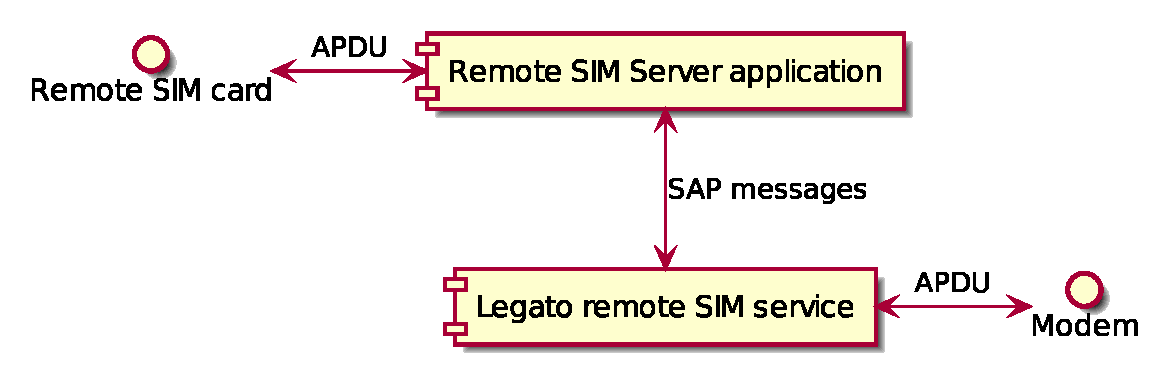
\includegraphics[width=\textwidth,height=\textheight/2,keepaspectratio=true]{le_rsim_Overview}}
\end{DoxyImageNoCaption}


\begin{DoxyNote}{Note}
The remote S\+IM Server application is not part of the Legato implementation and should be developed by the user.
\end{DoxyNote}
\hypertarget{c_rsim_le_rsim_binding}{}\subparagraph{I\+P\+C interfaces binding}\label{c_rsim_le_rsim_binding}
All the functions of this A\+PI are provided by the {\bfseries modem\+Service} application service.

Here\textquotesingle{}s a code sample binding to Data Connection services\+: \begin{DoxyVerb}bindings:
{
   clientExe.clientComponent.le_rsim -> modemService.le_rsim
}
\end{DoxyVerb}
\hypertarget{c_rsim_le_rsim_Communication}{}\subparagraph{Communication}\label{c_rsim_le_rsim_Communication}
The communication between the application and the remote S\+IM service uses the S\+IM Access Profile (S\+AP) protocol.

The latest \href{https://www.bluetooth.org/DocMan/handlers/DownloadDoc.ashx?doc_id=158740}{\tt V11r00 S\+AP specification} is supported by the remote S\+IM service. All client-\/mandatory features and some optional features are supported. The table below summarizes all S\+AP messages supported by the remote S\+IM service. \tabulinesep=1mm
\begin{longtabu} spread 0pt [c]{*4{|X[-1]}|}
\hline
\rowcolor{\tableheadbgcolor}{\bf Feature }&{\bf Associated S\+AP messages }&{\bf Support in S\+AP client }&{\bf R\+S\+IM support }\\\cline{1-4}
\endfirsthead
\hline
\endfoot
\hline
\rowcolor{\tableheadbgcolor}{\bf Feature }&{\bf Associated S\+AP messages }&{\bf Support in S\+AP client }&{\bf R\+S\+IM support }\\\cline{1-4}
\endhead
\multirow{5}{\linewidth}{Connection management }&C\+O\+N\+N\+E\+C\+T\+\_\+\+R\+EQ &\multirow{5}{\linewidth}{Mandatory }&Supported \\\cline{2-2}\cline{4-4}
&C\+O\+N\+N\+E\+C\+T\+\_\+\+R\+E\+SP &&Supported \\\cline{2-2}\cline{4-4}
&D\+I\+S\+C\+O\+N\+N\+E\+C\+T\+\_\+\+R\+EQ &&Supported \\\cline{2-2}\cline{4-4}
&D\+I\+S\+C\+O\+N\+N\+E\+C\+T\+\_\+\+R\+E\+SP &&Supported \\\cline{2-2}\cline{4-4}
&D\+I\+S\+C\+O\+N\+N\+E\+C\+T\+\_\+\+I\+ND &&Supported \\\cline{1-4}
\multirow{2}{\linewidth}{Transfer A\+P\+DU }&T\+R\+A\+N\+S\+F\+E\+R\+\_\+\+A\+P\+D\+U\+\_\+\+R\+EQ &\multirow{2}{\linewidth}{Mandatory }&Supported \\\cline{2-2}\cline{4-4}
&T\+R\+A\+N\+S\+F\+E\+R\+\_\+\+A\+P\+D\+U\+\_\+\+R\+E\+SP &&Supported \\\cline{1-4}
\multirow{2}{\linewidth}{Transfer A\+TR }&T\+R\+A\+N\+S\+F\+E\+R\+\_\+\+A\+T\+R\+\_\+\+R\+EQ &\multirow{2}{\linewidth}{Mandatory }&Supported \\\cline{2-2}\cline{4-4}
&T\+R\+A\+N\+S\+F\+E\+R\+\_\+\+A\+T\+R\+\_\+\+R\+E\+SP &&Supported \\\cline{1-4}
\multirow{2}{\linewidth}{Power S\+IM off }&P\+O\+W\+E\+R\+\_\+\+S\+I\+M\+\_\+\+O\+F\+F\+\_\+\+R\+EQ &\multirow{2}{\linewidth}{Optional }&Supported \\\cline{2-2}\cline{4-4}
&P\+O\+W\+E\+R\+\_\+\+S\+I\+M\+\_\+\+O\+F\+F\+\_\+\+R\+E\+SP &&Supported \\\cline{1-4}
\multirow{2}{\linewidth}{Power S\+IM on }&P\+O\+W\+E\+R\+\_\+\+S\+I\+M\+\_\+\+O\+N\+\_\+\+R\+EQ &\multirow{2}{\linewidth}{Mandatory }&Supported \\\cline{2-2}\cline{4-4}
&P\+O\+W\+E\+R\+\_\+\+S\+I\+M\+\_\+\+O\+N\+\_\+\+R\+E\+SP &&Supported \\\cline{1-4}
\multirow{2}{\linewidth}{Reset S\+IM }&R\+E\+S\+E\+T\+\_\+\+S\+I\+M\+\_\+\+R\+EQ &\multirow{2}{\linewidth}{Optional }&Supported \\\cline{2-2}\cline{4-4}
&R\+E\+S\+E\+T\+\_\+\+S\+I\+M\+\_\+\+R\+E\+SP &&Supported \\\cline{1-4}
Report Status &S\+T\+A\+T\+U\+S\+\_\+\+I\+ND &Mandatory &Supported \\\cline{1-4}
\multirow{2}{\linewidth}{Transfer Card Reader Status }&T\+R\+A\+N\+S\+F\+E\+R\+\_\+\+C\+A\+R\+D\+\_\+\+R\+E\+A\+D\+E\+R\+\_\+\+S\+T\+A\+T\+U\+S\+\_\+\+R\+EQ &\multirow{2}{\linewidth}{Optional }&Not supported \\\cline{2-2}\cline{4-4}
&T\+R\+A\+N\+S\+F\+E\+R\+\_\+\+C\+A\+R\+D\+\_\+\+R\+E\+A\+D\+E\+R\+\_\+\+S\+T\+A\+T\+U\+S\+\_\+\+R\+E\+SP &&Not supported \\\cline{1-4}
Error handling &E\+R\+R\+O\+R\+\_\+\+R\+E\+SP &Mandatory &Supported \\\cline{1-4}
\multirow{2}{\linewidth}{Set Transport Protocol }&S\+E\+T\+\_\+\+T\+R\+A\+N\+S\+P\+O\+R\+T\+\_\+\+P\+R\+O\+T\+O\+C\+O\+L\+\_\+\+R\+EQ &\multirow{2}{\linewidth}{Optional }&Not supported \\\cline{2-2}\cline{4-4}
&S\+E\+T\+\_\+\+T\+R\+A\+N\+S\+P\+O\+R\+T\+\_\+\+P\+R\+O\+T\+O\+C\+O\+L\+\_\+\+R\+E\+SP &&Not supported \\\cline{1-4}
\end{longtabu}


The application must register a handler function with \hyperlink{le__rsim__interface_8h_a7c525d3f8a02a4ca14e4fb723b6cc673}{le\+\_\+rsim\+\_\+\+Add\+Message\+Handler()} in order to receive the S\+AP messages sent by the remote S\+IM service. Registering the handler indicates that the remote S\+IM server is ready to receive messages and that a remote S\+IM card is available. The handler can be deregistered through the \hyperlink{le__rsim__interface_8h_ad488fe9d57c161a8c17ac60bda891817}{le\+\_\+rsim\+\_\+\+Remove\+Message\+Handler()} function when it is not needed anymore.

The application can send S\+AP messages to the remote S\+IM service with the \hyperlink{le__rsim__interface_8h_ace5e9e861ab59d4ec8e6198b827a5c28}{le\+\_\+rsim\+\_\+\+Send\+Message()} function. Message sending is an asynchronous process\+: a callback can therefore be passed to \hyperlink{le__rsim__interface_8h_ace5e9e861ab59d4ec8e6198b827a5c28}{le\+\_\+rsim\+\_\+\+Send\+Message()} in order to receive the sending result for this message.

\begin{DoxyWarning}{Warning}
The remote S\+IM service supports only one remote S\+IM card and can therefore be connected with only one application.
\end{DoxyWarning}
\begin{DoxyNote}{Note}

\begin{DoxyItemize}
\item The remote S\+IM service has to be supported by the modem to be used\+: check your platform documentation.
\item The remote S\+IM card should be selected in order to use the remote S\+IM service.
\item As runtime switch is not currently supported, the switch between local and remote S\+IM card requires a platform reset to take effect.
\end{DoxyItemize}
\end{DoxyNote}
A sample code of a basic remote S\+IM server is available in the following page\+:
\begin{DoxyItemize}
\item \hyperlink{c_rsimTest}{Sample code}
\end{DoxyItemize}





Copyright (C) Sierra Wireless Inc. \hypertarget{c_rsimTest}{}\paragraph{Sample code}\label{c_rsimTest}

\begin{DoxyCodeInclude}
\textcolor{comment}{ /**}
\textcolor{comment}{  * @file rsimTest.c}
\textcolor{comment}{  *}
\textcolor{comment}{  * This application implements a basic remote SIM server using the Legato remote SIM service.}
\textcolor{comment}{  *}
\textcolor{comment}{  * No physical remote SIM card is connected or supported by this server and all SIM responses}
\textcolor{comment}{  * are simulated. This application is therefore only used for sanity tests.}
\textcolor{comment}{  *}
\textcolor{comment}{  * The remote SIM server does the following:}
\textcolor{comment}{  * - Register a RSIM message handler}
\textcolor{comment}{  * - Receive a SAP connection request, establish the connection and send the ATR}
\textcolor{comment}{  * - Receive a first APDU request and respond with an APDU response error}
\textcolor{comment}{  * - Receive a second APDU request and respond with a correct APDU response}
\textcolor{comment}{  * - Receive a third APDU request and trigger a graceful SAP disconnection}
\textcolor{comment}{  * - Exit}
\textcolor{comment}{  *}
\textcolor{comment}{  * @note}
\textcolor{comment}{  * - Ensure that your platform supports the remote SIM service before using it}
\textcolor{comment}{  * - Select the remote SIM card and reboot before using it}
\textcolor{comment}{  * - The application does not start automatically and should be started with "app start rsimTest"}
\textcolor{comment}{  *}
\textcolor{comment}{  * <HR>}
\textcolor{comment}{  *}
\textcolor{comment}{  * Copyright (C) Sierra Wireless Inc.}
\textcolor{comment}{  */}

\textcolor{preprocessor}{#include "\hyperlink{legato_8h}{legato.h}"}
\textcolor{preprocessor}{#include "interfaces.h"}


\textcolor{comment}{//--------------------------------------------------------------------------------------------------}
\textcolor{comment}{// Symbol and Enum definitions}
\textcolor{comment}{//--------------------------------------------------------------------------------------------------}

\textcolor{comment}{//--------------------------------------------------------------------------------------------------}\textcolor{comment}{}
\textcolor{comment}{/**}
\textcolor{comment}{ * Memory pool size}
\textcolor{comment}{ */}
\textcolor{comment}{//--------------------------------------------------------------------------------------------------}
\textcolor{preprocessor}{#define RSIM\_EVENTS\_POOL\_SIZE   2}

\textcolor{comment}{//--------------------------------------------------------------------------------------------------}\textcolor{comment}{}
\textcolor{comment}{/**}
\textcolor{comment}{ * SAP message identifiers (cf. SIM Access Profile specification)}
\textcolor{comment}{ */}
\textcolor{comment}{//--------------------------------------------------------------------------------------------------}
\textcolor{preprocessor}{#define SAP\_MSGID\_CONNECT\_REQ                       0x00}
\textcolor{preprocessor}{#define SAP\_MSGID\_CONNECT\_RESP                      0x01}
\textcolor{preprocessor}{#define SAP\_MSGID\_DISCONNECT\_REQ                    0x02}
\textcolor{preprocessor}{#define SAP\_MSGID\_DISCONNECT\_RESP                   0x03}
\textcolor{preprocessor}{#define SAP\_MSGID\_DISCONNECT\_IND                    0x04}
\textcolor{preprocessor}{#define SAP\_MSGID\_TRANSFER\_APDU\_REQ                 0x05}
\textcolor{preprocessor}{#define SAP\_MSGID\_TRANSFER\_APDU\_RESP                0x06}
\textcolor{preprocessor}{#define SAP\_MSGID\_TRANSFER\_ATR\_REQ                  0x07}
\textcolor{preprocessor}{#define SAP\_MSGID\_TRANSFER\_ATR\_RESP                 0x08}
\textcolor{preprocessor}{#define SAP\_MSGID\_POWER\_SIM\_OFF\_REQ                 0x09}
\textcolor{preprocessor}{#define SAP\_MSGID\_POWER\_SIM\_OFF\_RESP                0x0A}
\textcolor{preprocessor}{#define SAP\_MSGID\_POWER\_SIM\_ON\_REQ                  0x0B}
\textcolor{preprocessor}{#define SAP\_MSGID\_POWER\_SIM\_ON\_RESP                 0x0C}
\textcolor{preprocessor}{#define SAP\_MSGID\_RESET\_SIM\_REQ                     0x0D}
\textcolor{preprocessor}{#define SAP\_MSGID\_RESET\_SIM\_RESP                    0x0E}
\textcolor{preprocessor}{#define SAP\_MSGID\_TRANSFER\_CARD\_READER\_STATUS\_REQ   0x0F}
\textcolor{preprocessor}{#define SAP\_MSGID\_TRANSFER\_CARD\_READER\_STATUS\_RESP  0x10}
\textcolor{preprocessor}{#define SAP\_MSGID\_STATUS\_IND                        0x11}
\textcolor{preprocessor}{#define SAP\_MSGID\_ERROR\_RESP                        0x12}
\textcolor{preprocessor}{#define SAP\_MSGID\_SET\_TRANSPORT\_PROTOCOL\_REQ        0x13}
\textcolor{preprocessor}{#define SAP\_MSGID\_SET\_TRANSPORT\_PROTOCOL\_RESP       0x14}

\textcolor{comment}{//--------------------------------------------------------------------------------------------------}\textcolor{comment}{}
\textcolor{comment}{/**}
\textcolor{comment}{ * SAP parameters identifiers (cf. SIM Access Profile specification)}
\textcolor{comment}{ */}
\textcolor{comment}{//--------------------------------------------------------------------------------------------------}
\textcolor{preprocessor}{#define SAP\_PARAMID\_MAX\_MSG\_SIZE            0x00}
\textcolor{preprocessor}{#define SAP\_PARAMID\_CONNECTION\_STATUS       0x01}
\textcolor{preprocessor}{#define SAP\_PARAMID\_RESULT\_CODE             0x02}
\textcolor{preprocessor}{#define SAP\_PARAMID\_DISCONNECTION\_TYPE      0x03}
\textcolor{preprocessor}{#define SAP\_PARAMID\_COMMAND\_APDU            0x04}
\textcolor{preprocessor}{#define SAP\_PARAMID\_COMMAND\_APDU\_7816       0x10}
\textcolor{preprocessor}{#define SAP\_PARAMID\_RESPONSE\_APDU           0x05}
\textcolor{preprocessor}{#define SAP\_PARAMID\_ATR                     0x06}
\textcolor{preprocessor}{#define SAP\_PARAMID\_CARD\_READER\_STATUS      0x07}
\textcolor{preprocessor}{#define SAP\_PARAMID\_STATUS\_CHANGE           0x08}
\textcolor{preprocessor}{#define SAP\_PARAMID\_TRANSPORT\_PROTOCOL      0x09}

\textcolor{comment}{//--------------------------------------------------------------------------------------------------}\textcolor{comment}{}
\textcolor{comment}{/**}
\textcolor{comment}{ * Length in bytes of different parameters of SAP messages (cf. SIM Access Profile specification).}
\textcolor{comment}{ * Only parameters with fixed lengths are listed here}
\textcolor{comment}{ */}
\textcolor{comment}{//--------------------------------------------------------------------------------------------------}
\textcolor{preprocessor}{#define SAP\_LENGTH\_SAP\_HEADER           4   }\textcolor{comment}{///< 4 bytes header for SAP messages}
\textcolor{comment}{}#define SAP\_LENGTH\_PARAM\_HEADER         4   \textcolor{comment}{///< 4 bytes header for each parameter}
\textcolor{comment}{}#define SAP\_LENGTH\_MAX\_MSG\_SIZE         2
\textcolor{preprocessor}{#define SAP\_LENGTH\_CONNECTION\_STATUS    1}
\textcolor{preprocessor}{#define SAP\_LENGTH\_RESULT\_CODE          1}
\textcolor{preprocessor}{#define SAP\_LENGTH\_DISCONNECTION\_TYPE   1}
\textcolor{preprocessor}{#define SAP\_LENGTH\_CARD\_READER\_STATUS   1}
\textcolor{preprocessor}{#define SAP\_LENGTH\_STATUS\_CHANGE        1}
\textcolor{preprocessor}{#define SAP\_LENGTH\_TRANSPORT\_PROTOCOL   1}
\textcolor{preprocessor}{#define SAP\_LENGTH\_PARAM\_PAYLOAD        4   }\textcolor{comment}{///< Parameter payload is 4 bytes long with padding}
\textcolor{comment}{}#define SAP\_LENGTH\_PARAM                (SAP\_LENGTH\_PARAM\_HEADER + SAP\_LENGTH\_PARAM\_PAYLOAD)

\textcolor{comment}{//--------------------------------------------------------------------------------------------------}\textcolor{comment}{}
\textcolor{comment}{/**}
\textcolor{comment}{ * SAP ConnectionStatus values (cf. SIM Access Profile specification section 5.2.2)}
\textcolor{comment}{ */}
\textcolor{comment}{//--------------------------------------------------------------------------------------------------}
\textcolor{preprocessor}{#define SAP\_CONNSTATUS\_OK               0x00    }\textcolor{comment}{///< OK, Server can fulfill requirements}
\textcolor{comment}{}#define SAP\_CONNSTATUS\_SERVER\_NOK       0x01    \textcolor{comment}{///< Error, Server unable to establish connection}
\textcolor{comment}{}#define SAP\_CONNSTATUS\_MAXMSGSIZE\_NOK   0x02    \textcolor{comment}{///< Error, Server does not support}
\textcolor{comment}{}\textcolor{comment}{                                                ///< maximum message size}
\textcolor{comment}{}#define SAP\_CONNSTATUS\_SMALL\_MAXMSGSIZE 0x03    \textcolor{comment}{///< Error, maximum message size}
\textcolor{comment}{}\textcolor{comment}{                                                ///< by Client is too small}
\textcolor{comment}{}#define SAP\_CONNSTATUS\_OK\_ONGOING\_CALL  0x04    \textcolor{comment}{///< OK, ongoing call}
\textcolor{comment}{}
\textcolor{comment}{//--------------------------------------------------------------------------------------------------}\textcolor{comment}{}
\textcolor{comment}{/**}
\textcolor{comment}{ * SAP DisconnectionType values (cf. SIM Access Profile specification section 5.2.3)}
\textcolor{comment}{ */}
\textcolor{comment}{//--------------------------------------------------------------------------------------------------}
\textcolor{preprocessor}{#define SAP\_DISCONNTYPE\_GRACEFUL        0x00    }\textcolor{comment}{///< Graceful}
\textcolor{comment}{}#define SAP\_DISCONNTYPE\_IMMEDIATE       0x01    \textcolor{comment}{///< Immediate}
\textcolor{comment}{}
\textcolor{comment}{//--------------------------------------------------------------------------------------------------}\textcolor{comment}{}
\textcolor{comment}{/**}
\textcolor{comment}{ * SAP ResultCode values (cf. SIM Access Profile specification section 5.2.4)}
\textcolor{comment}{ */}
\textcolor{comment}{//--------------------------------------------------------------------------------------------------}
\textcolor{preprocessor}{#define SAP\_RESULTCODE\_OK                   0x00    }\textcolor{comment}{///< OK, request processed correctly}
\textcolor{comment}{}#define SAP\_RESULTCODE\_ERROR\_NO\_REASON      0x01    \textcolor{comment}{///< Error, no reason defined}
\textcolor{comment}{}#define SAP\_RESULTCODE\_ERROR\_CARD\_NOK       0x02    \textcolor{comment}{///< Error, card not accessible}
\textcolor{comment}{}#define SAP\_RESULTCODE\_ERROR\_CARD\_OFF       0x03    \textcolor{comment}{///< Error, card (already) powered off}
\textcolor{comment}{}#define SAP\_RESULTCODE\_ERROR\_CARD\_REMOVED   0x04    \textcolor{comment}{///< Error, card removed}
\textcolor{comment}{}#define SAP\_RESULTCODE\_ERROR\_CARD\_ON        0x05    \textcolor{comment}{///< Error, card already powered on}
\textcolor{comment}{}#define SAP\_RESULTCODE\_ERROR\_NO\_DATA        0x06    \textcolor{comment}{///< Error, data not available}
\textcolor{comment}{}#define SAP\_RESULTCODE\_ERROR\_NOT\_SUPPORTED  0x07    \textcolor{comment}{///< Error, not supported}
\textcolor{comment}{}
\textcolor{comment}{//--------------------------------------------------------------------------------------------------}\textcolor{comment}{}
\textcolor{comment}{/**}
\textcolor{comment}{ * SAP StatusChange values (cf. SIM Access Profile specification section 5.2.8)}
\textcolor{comment}{ */}
\textcolor{comment}{//--------------------------------------------------------------------------------------------------}
\textcolor{preprocessor}{#define SAP\_STATUSCHANGE\_UNKNOWN\_ERROR  0x00    }\textcolor{comment}{///< Unknown Error}
\textcolor{comment}{}#define SAP\_STATUSCHANGE\_CARD\_RESET     0x01    \textcolor{comment}{///< Card reset}
\textcolor{comment}{}#define SAP\_STATUSCHANGE\_CARD\_NOK       0x02    \textcolor{comment}{///< Card not accessible}
\textcolor{comment}{}#define SAP\_STATUSCHANGE\_CARD\_REMOVED   0x03    \textcolor{comment}{///< Card removed}
\textcolor{comment}{}#define SAP\_STATUSCHANGE\_CARD\_INSERTED  0x04    \textcolor{comment}{///< Card inserted}
\textcolor{comment}{}#define SAP\_STATUSCHANGE\_CARD\_RECOVERED 0x05    \textcolor{comment}{///< Card recovered}
\textcolor{comment}{}
\textcolor{comment}{//--------------------------------------------------------------------------------------------------}\textcolor{comment}{}
\textcolor{comment}{/**}
\textcolor{comment}{ * Bit shift to access MSB byte}
\textcolor{comment}{ */}
\textcolor{comment}{//--------------------------------------------------------------------------------------------------}
\textcolor{preprocessor}{#define MSB\_SHIFT   8}


\textcolor{comment}{//--------------------------------------------------------------------------------------------------}
\textcolor{comment}{// Data structures}
\textcolor{comment}{//--------------------------------------------------------------------------------------------------}

\textcolor{comment}{//--------------------------------------------------------------------------------------------------}\textcolor{comment}{}
\textcolor{comment}{/**}
\textcolor{comment}{ * RSIM message sending structure}
\textcolor{comment}{ */}
\textcolor{comment}{//--------------------------------------------------------------------------------------------------}
\textcolor{keyword}{typedef} \textcolor{keyword}{struct}
\{
    uint8\_t message[\hyperlink{le__rsim__interface_8h_a6e8b290ec4404fd2a7b6c119d82dc9ef}{LE\_RSIM\_MAX\_MSG\_SIZE}];      \textcolor{comment}{///< Message}
\textcolor{comment}{}    \textcolor{keywordtype}{size\_t}  messageSize;                        \textcolor{comment}{///< Message size}
\textcolor{comment}{}    \hyperlink{le__rsim__interface_8h_afc68d9993eb6b20a697cdabfe85c0843}{le\_rsim\_CallbackHandlerFunc\_t} callbackPtr;  \textcolor{comment}{///< Callback response}
\textcolor{comment}{}    \textcolor{keywordtype}{void}*   context;                            \textcolor{comment}{///< Associated context}
\textcolor{comment}{}\}
RsimMessageSending\_t;


\textcolor{comment}{//--------------------------------------------------------------------------------------------------}
\textcolor{comment}{// Static declarations}
\textcolor{comment}{//--------------------------------------------------------------------------------------------------}

\textcolor{comment}{//--------------------------------------------------------------------------------------------------}\textcolor{comment}{}
\textcolor{comment}{/**}
\textcolor{comment}{ * Memory pool used to transfer RSIM messages sending to the application thread}
\textcolor{comment}{ */}
\textcolor{comment}{//--------------------------------------------------------------------------------------------------}
\textcolor{keyword}{static} le\_mem\_PoolRef\_t RsimMessagesPool;

\textcolor{comment}{//--------------------------------------------------------------------------------------------------}\textcolor{comment}{}
\textcolor{comment}{/**}
\textcolor{comment}{ *  RSIM message handler reference}
\textcolor{comment}{ */}
\textcolor{comment}{//--------------------------------------------------------------------------------------------------}
\textcolor{keyword}{static} \hyperlink{le__rsim__interface_8h_a5da55c94a0910d5334e680d824dc7fa2}{le\_rsim\_MessageHandlerRef\_t} RsimMessageHandlerRef;

\textcolor{comment}{//--------------------------------------------------------------------------------------------------}\textcolor{comment}{}
\textcolor{comment}{/**}
\textcolor{comment}{ *  Semaphore used to synchronize the test}
\textcolor{comment}{ */}
\textcolor{comment}{//--------------------------------------------------------------------------------------------------}
\textcolor{keyword}{static} \hyperlink{le__semaphore_8h_a25b1300f952a83efe8ad0a321f2d06dc}{le\_sem\_Ref\_t} AppSemaphore;

\textcolor{comment}{//--------------------------------------------------------------------------------------------------}\textcolor{comment}{}
\textcolor{comment}{/**}
\textcolor{comment}{ *  Application thread reference}
\textcolor{comment}{ */}
\textcolor{comment}{//--------------------------------------------------------------------------------------------------}
\textcolor{keyword}{static} \hyperlink{le__thread_8h_a32121104c6b4ca39008eb79a4d6862f2}{le\_thread\_Ref\_t} AppThreadRef;

\textcolor{comment}{//--------------------------------------------------------------------------------------------------}\textcolor{comment}{}
\textcolor{comment}{/**}
\textcolor{comment}{ *  Expected message identifier}
\textcolor{comment}{ */}
\textcolor{comment}{//--------------------------------------------------------------------------------------------------}
\textcolor{keyword}{static} uint8\_t ExpectedMessageId = 0;


\textcolor{comment}{//--------------------------------------------------------------------------------------------------}
\textcolor{comment}{// Utility functions}
\textcolor{comment}{//--------------------------------------------------------------------------------------------------}

\textcolor{comment}{// -------------------------------------------------------------------------------------------------}\textcolor{comment}{}
\textcolor{comment}{/**}
\textcolor{comment}{ *  Callback for RSIM messages sending result}
\textcolor{comment}{ */}
\textcolor{comment}{// -------------------------------------------------------------------------------------------------}
\textcolor{keyword}{static} \textcolor{keywordtype}{void} CallbackHandler
(
    uint8\_t messageId,
    \hyperlink{le__basics_8h_a1cca095ed6ebab24b57a636382a6c86c}{le\_result\_t} result,
    \textcolor{keywordtype}{void}* contextPtr
)
\{
    \hyperlink{le__log_8h_a2a91ea8857cf190fde71d85ba930a498}{LE\_DEBUG}(\textcolor{stringliteral}{"Sending result: messageId=%d, result=%d, context=%p"}, messageId, result, contextPtr);

    \textcolor{comment}{// Check sending result against expected result}
    \hyperlink{le__log_8h_ac0dbbef91dc0fed449d0092ff0557b39}{LE\_ASSERT}(result == (\hyperlink{le__basics_8h_a1cca095ed6ebab24b57a636382a6c86c}{le\_result\_t})contextPtr)

    \hyperlink{le__semaphore_8h_abb859411cc58fbcc576c986ef52083b2}{le\_sem\_Post}(AppSemaphore);
\}

\textcolor{comment}{//--------------------------------------------------------------------------------------------------}\textcolor{comment}{}
\textcolor{comment}{/**}
\textcolor{comment}{ *  Send SAP message through application thread}
\textcolor{comment}{ */}
\textcolor{comment}{//--------------------------------------------------------------------------------------------------}
\textcolor{keyword}{static} \textcolor{keywordtype}{void} SendSapMessage
(
    \textcolor{keywordtype}{void}* param1Ptr,
    \textcolor{keywordtype}{void}* param2Ptr
)
\{
    RsimMessageSending\_t* rsimSendingPtr = (RsimMessageSending\_t*) param1Ptr;

    \textcolor{comment}{// Send message}
    \hyperlink{le__log_8h_a7cd2daa3d4af1de4d29e0eed95187484}{LE\_ASSERT\_OK}(\hyperlink{le__rsim__interface_8h_ace5e9e861ab59d4ec8e6198b827a5c28}{le\_rsim\_SendMessage}(rsimSendingPtr->message,
                                     rsimSendingPtr->messageSize,
                                     rsimSendingPtr->callbackPtr,
                                     rsimSendingPtr->context));

    \textcolor{comment}{// Release allocated memory}
    \hyperlink{le__mem_8h_a6d8e3fe430bcb81efe97b57ce30ef2de}{le\_mem\_Release}(rsimSendingPtr);
\}

\textcolor{comment}{//--------------------------------------------------------------------------------------------------}\textcolor{comment}{}
\textcolor{comment}{/**}
\textcolor{comment}{ *  Send SAP CONNECT\_RESP message}
\textcolor{comment}{ */}
\textcolor{comment}{//--------------------------------------------------------------------------------------------------}
\textcolor{keyword}{static} \textcolor{keywordtype}{void} SendSapConnectResp
(
    uint8\_t  connectionStatus,
    uint16\_t maxMsgSize
)
\{
    uint8\_t message[\hyperlink{le__rsim__interface_8h_a6e8b290ec4404fd2a7b6c119d82dc9ef}{LE\_RSIM\_MAX\_MSG\_SIZE}];
    \textcolor{keywordtype}{size\_t}  messageSize = 0;
    memset(&message, 0, \textcolor{keyword}{sizeof}(message));

    \textcolor{comment}{// ConnectionStatus 'Error, Server does not support maximum message size'}
    \textcolor{keywordflow}{if} (SAP\_CONNSTATUS\_MAXMSGSIZE\_NOK == connectionStatus)
    \{
        \textcolor{comment}{// SAP header}
        message[0]  = SAP\_MSGID\_CONNECT\_RESP;               \textcolor{comment}{// MsgId (CONNECT\_RESP)}
        message[1]  = 0x02;                                 \textcolor{comment}{// Parameters number}
        message[2]  = 0x00;                                 \textcolor{comment}{// Reserved}
        message[3]  = 0x00;                                 \textcolor{comment}{// Reserved}

        \textcolor{comment}{// Parameter header}
        message[4]  = SAP\_PARAMID\_CONNECTION\_STATUS;        \textcolor{comment}{// Parameter Id}
        message[5]  = 0x00;                                 \textcolor{comment}{// Reserved}
        message[6]  = 0x00;                                 \textcolor{comment}{// Parameter length (MSB)}
        message[7]  = SAP\_LENGTH\_CONNECTION\_STATUS;         \textcolor{comment}{// Parameter length (LSB)}

        \textcolor{comment}{// Parameter value (ConnectionStatus)}
        message[8]  = connectionStatus;                     \textcolor{comment}{// ConnectionStatus}
        message[9]  = 0x00;                                 \textcolor{comment}{// Padding}
        message[10] = 0x00;                                 \textcolor{comment}{// Padding}
        message[11] = 0x00;                                 \textcolor{comment}{// Padding}

        \textcolor{comment}{// Parameter header}
        message[12] = SAP\_PARAMID\_MAX\_MSG\_SIZE;             \textcolor{comment}{// Parameter Id}
        message[13] = 0x00;                                 \textcolor{comment}{// Reserved}
        message[14] = 0x00;                                 \textcolor{comment}{// Parameter length (MSB)}
        message[15] = SAP\_LENGTH\_MAX\_MSG\_SIZE;              \textcolor{comment}{// Parameter length (LSB)}

        \textcolor{comment}{// Parameter value (MaxMsgSize)}
        message[16] = ((maxMsgSize & 0xFF00U) >> MSB\_SHIFT);\textcolor{comment}{// MaxMsgSize (MSB)}
        message[17] = (maxMsgSize & 0x00FF);                \textcolor{comment}{// MaxMsgSize (LSB)}
        message[18] = 0x00;                                 \textcolor{comment}{// Padding}
        message[19] = 0x00;                                 \textcolor{comment}{// Padding}

        \textcolor{comment}{// Message size}
        messageSize = 20;
    \}
    \textcolor{keywordflow}{else}
    \{
        \textcolor{comment}{// SAP header}
        message[0]  = SAP\_MSGID\_CONNECT\_RESP;           \textcolor{comment}{// MsgId (CONNECT\_RESP)}
        message[1]  = 0x01;                             \textcolor{comment}{// Parameters number}
        message[2]  = 0x00;                             \textcolor{comment}{// Reserved}
        message[3]  = 0x00;                             \textcolor{comment}{// Reserved}

        \textcolor{comment}{// Parameter header}
        message[4]  = SAP\_PARAMID\_CONNECTION\_STATUS;    \textcolor{comment}{// Parameter Id}
        message[5]  = 0x00;                             \textcolor{comment}{// Reserved}
        message[6]  = 0x00;                             \textcolor{comment}{// Parameter length (MSB)}
        message[7]  = SAP\_LENGTH\_CONNECTION\_STATUS;     \textcolor{comment}{// Parameter length (LSB)}

        \textcolor{comment}{// Parameter value (ConnectionStatus)}
        message[8]  = connectionStatus;                 \textcolor{comment}{// ConnectionStatus}
        message[9]  = 0x00;                             \textcolor{comment}{// Padding}
        message[10] = 0x00;                             \textcolor{comment}{// Padding}
        message[11] = 0x00;                             \textcolor{comment}{// Padding}

        \textcolor{comment}{// Message size}
        messageSize = 12;
    \}

    \hyperlink{le__log_8h_a2a91ea8857cf190fde71d85ba930a498}{LE\_DEBUG}(\textcolor{stringliteral}{"Send CONNECT\_RESP message:"});
    \hyperlink{le__log_8h_a2949aa2907a8390e5c93421f42432e26}{LE\_DUMP}(message, messageSize);

    \textcolor{comment}{// Send message with the application thread}
    RsimMessageSending\_t* rsimSendingPtr = \hyperlink{le__mem_8h_af7c289c73d4182835a26a9099f3db359}{le\_mem\_ForceAlloc}(RsimMessagesPool);
    memcpy(rsimSendingPtr->message, message, messageSize);
    rsimSendingPtr->messageSize = messageSize;
    rsimSendingPtr->callbackPtr = CallbackHandler;
    rsimSendingPtr->context = (\textcolor{keywordtype}{void}*)LE\_OK;
    \hyperlink{le__event_loop_8h_a228da2d1f53ffa74517f108b0dcfa4d9}{le\_event\_QueueFunctionToThread}(AppThreadRef, SendSapMessage, 
      rsimSendingPtr, NULL);
\}

\textcolor{comment}{//--------------------------------------------------------------------------------------------------}\textcolor{comment}{}
\textcolor{comment}{/**}
\textcolor{comment}{ *  Send SAP STATUS\_IND message}
\textcolor{comment}{ */}
\textcolor{comment}{//--------------------------------------------------------------------------------------------------}
\textcolor{keyword}{static} \textcolor{keywordtype}{void} SendSapStatusInd
(
    uint8\_t statusChange
)
\{
    uint8\_t message[\hyperlink{le__rsim__interface_8h_a6e8b290ec4404fd2a7b6c119d82dc9ef}{LE\_RSIM\_MAX\_MSG\_SIZE}];
    \textcolor{keywordtype}{size\_t}  messageSize = 0;
    memset(&message, 0, \textcolor{keyword}{sizeof}(message));

    \textcolor{comment}{// SAP header}
    message[0]  = SAP\_MSGID\_STATUS\_IND;         \textcolor{comment}{// MsgId (STATUS\_IND)}
    message[1]  = 0x01;                         \textcolor{comment}{// Parameters number}
    message[2]  = 0x00;                         \textcolor{comment}{// Reserved}
    message[3]  = 0x00;                         \textcolor{comment}{// Reserved}

    \textcolor{comment}{// Parameter header}
    message[4]  = SAP\_PARAMID\_STATUS\_CHANGE;    \textcolor{comment}{// Parameter Id}
    message[5]  = 0x00;                         \textcolor{comment}{// Reserved}
    message[6]  = 0x00;                         \textcolor{comment}{// Parameter length (MSB)}
    message[7]  = SAP\_LENGTH\_STATUS\_CHANGE;     \textcolor{comment}{// Parameter length (LSB)}

    \textcolor{comment}{// Parameter value (StatusChange)}
    message[8]  = statusChange;                 \textcolor{comment}{// StatusChange}
    message[9]  = 0x00;                         \textcolor{comment}{// Padding}
    message[10] = 0x00;                         \textcolor{comment}{// Padding}
    message[11] = 0x00;                         \textcolor{comment}{// Padding}

    \textcolor{comment}{// Message size}
    messageSize = 12;

    \hyperlink{le__log_8h_a2a91ea8857cf190fde71d85ba930a498}{LE\_DEBUG}(\textcolor{stringliteral}{"Send STATUS\_IND message:"});
    \hyperlink{le__log_8h_a2949aa2907a8390e5c93421f42432e26}{LE\_DUMP}(message, messageSize);

    \textcolor{comment}{// Send message with the application thread}
    RsimMessageSending\_t* rsimSendingPtr = \hyperlink{le__mem_8h_af7c289c73d4182835a26a9099f3db359}{le\_mem\_ForceAlloc}(RsimMessagesPool);
    memcpy(rsimSendingPtr->message, message, messageSize);
    rsimSendingPtr->messageSize = messageSize;
    rsimSendingPtr->callbackPtr = CallbackHandler;
    rsimSendingPtr->context = (\textcolor{keywordtype}{void}*)LE\_OK;
    \hyperlink{le__event_loop_8h_a228da2d1f53ffa74517f108b0dcfa4d9}{le\_event\_QueueFunctionToThread}(AppThreadRef, SendSapMessage, 
      rsimSendingPtr, NULL);
\}

\textcolor{comment}{//--------------------------------------------------------------------------------------------------}\textcolor{comment}{}
\textcolor{comment}{/**}
\textcolor{comment}{ *  Send SAP TRANSFER\_ATR\_RESP message}
\textcolor{comment}{ */}
\textcolor{comment}{//--------------------------------------------------------------------------------------------------}
\textcolor{keyword}{static} \textcolor{keywordtype}{void} SendSapTransferAtrResp
(
    uint8\_t  resultCode,
    uint8\_t* atrPtr,
    uint16\_t atrLen
)
\{
    uint8\_t message[\hyperlink{le__rsim__interface_8h_a6e8b290ec4404fd2a7b6c119d82dc9ef}{LE\_RSIM\_MAX\_MSG\_SIZE}];
    \textcolor{keywordtype}{size\_t}  messageSize = 0;
    memset(&message, 0, \textcolor{keyword}{sizeof}(message));

    \textcolor{comment}{// ResultCode 'OK, request processed correctly'}
    \textcolor{keywordflow}{if} (SAP\_RESULTCODE\_OK == resultCode)
    \{
        \textcolor{comment}{// SAP header}
        message[0]  = SAP\_MSGID\_TRANSFER\_ATR\_RESP;      \textcolor{comment}{// MsgId (TRANSFER\_ATR\_RESP)}
        message[1]  = 0x02;                             \textcolor{comment}{// Parameters number}
        message[2]  = 0x00;                             \textcolor{comment}{// Reserved}
        message[3]  = 0x00;                             \textcolor{comment}{// Reserved}

        \textcolor{comment}{// Parameter header}
        message[4]  = SAP\_PARAMID\_RESULT\_CODE;          \textcolor{comment}{// Parameter Id}
        message[5]  = 0x00;                             \textcolor{comment}{// Reserved}
        message[6]  = 0x00;                             \textcolor{comment}{// Parameter length (MSB)}
        message[7]  = SAP\_LENGTH\_RESULT\_CODE;           \textcolor{comment}{// Parameter length (LSB)}

        \textcolor{comment}{// Parameter value (ResultCode)}
        message[8]  = resultCode;                       \textcolor{comment}{// ResultCode}
        message[9]  = 0x00;                             \textcolor{comment}{// Padding}
        message[10] = 0x00;                             \textcolor{comment}{// Padding}
        message[11] = 0x00;                             \textcolor{comment}{// Padding}

        \textcolor{comment}{// Parameter header}
        message[12] = SAP\_PARAMID\_ATR;                  \textcolor{comment}{// Parameter Id}
        message[13] = 0x00;                             \textcolor{comment}{// Reserved}
        message[14] = ((atrLen & 0xFF00U) >> MSB\_SHIFT);\textcolor{comment}{// Parameter length (MSB)}
        message[15] = (atrLen & 0x00FF);                \textcolor{comment}{// Parameter length (LSB)}

        \textcolor{comment}{// Current message size}
        messageSize = 16;

        \textcolor{comment}{// Parameter value (ATR)}
        memcpy(&message[messageSize], atrPtr, atrLen);
        messageSize += atrLen;

        \textcolor{comment}{// Message size should be 4-byte aligned}
        messageSize += (4 - (messageSize % 4));
    \}
    \textcolor{keywordflow}{else}
    \{
        \textcolor{comment}{// SAP header}
        message[0]  = SAP\_MSGID\_TRANSFER\_ATR\_RESP;  \textcolor{comment}{// MsgId (TRANSFER\_ATR\_RESP)}
        message[1]  = 0x01;                         \textcolor{comment}{// Parameters number}
        message[2]  = 0x00;                         \textcolor{comment}{// Reserved}
        message[3]  = 0x00;                         \textcolor{comment}{// Reserved}

        \textcolor{comment}{// Parameter header}
        message[4]  = SAP\_PARAMID\_RESULT\_CODE;      \textcolor{comment}{// Parameter Id}
        message[5]  = 0x00;                         \textcolor{comment}{// Reserved}
        message[6]  = 0x00;                         \textcolor{comment}{// Parameter length (MSB)}
        message[7]  = SAP\_LENGTH\_RESULT\_CODE;       \textcolor{comment}{// Parameter length (LSB)}

        \textcolor{comment}{// Parameter value (ResultCode)}
        message[8]  = resultCode;                   \textcolor{comment}{// ResultCode}
        message[9]  = 0x00;                         \textcolor{comment}{// Padding}
        message[10] = 0x00;                         \textcolor{comment}{// Padding}
        message[11] = 0x00;                         \textcolor{comment}{// Padding}

        \textcolor{comment}{// Message size}
        messageSize = 12;
    \}

    \hyperlink{le__log_8h_a2a91ea8857cf190fde71d85ba930a498}{LE\_DEBUG}(\textcolor{stringliteral}{"Send TRANSFER\_ATR\_RESP message:"});
    \hyperlink{le__log_8h_a2949aa2907a8390e5c93421f42432e26}{LE\_DUMP}(message, messageSize);

    \textcolor{comment}{// Send message with the application thread}
    RsimMessageSending\_t* rsimSendingPtr = \hyperlink{le__mem_8h_af7c289c73d4182835a26a9099f3db359}{le\_mem\_ForceAlloc}(RsimMessagesPool);
    memcpy(rsimSendingPtr->message, message, messageSize);
    rsimSendingPtr->messageSize = messageSize;
    rsimSendingPtr->callbackPtr = CallbackHandler;
    rsimSendingPtr->context = (\textcolor{keywordtype}{void}*)LE\_OK;
    \hyperlink{le__event_loop_8h_a228da2d1f53ffa74517f108b0dcfa4d9}{le\_event\_QueueFunctionToThread}(AppThreadRef, SendSapMessage, 
      rsimSendingPtr, NULL);
\}

\textcolor{comment}{//--------------------------------------------------------------------------------------------------}\textcolor{comment}{}
\textcolor{comment}{/**}
\textcolor{comment}{ *  Send SAP TRANSFER\_APDU\_RESP message}
\textcolor{comment}{ */}
\textcolor{comment}{//--------------------------------------------------------------------------------------------------}
\textcolor{keyword}{static} \textcolor{keywordtype}{void} SendSapTransferApduResp
(
    uint8\_t  resultCode,
    uint8\_t* apduPtr,
    uint16\_t apduLen
)
\{
    uint8\_t message[\hyperlink{le__rsim__interface_8h_a6e8b290ec4404fd2a7b6c119d82dc9ef}{LE\_RSIM\_MAX\_MSG\_SIZE}];
    \textcolor{keywordtype}{size\_t}  messageSize = 0;
    memset(&message, 0, \textcolor{keyword}{sizeof}(message));

    \textcolor{comment}{// ResultCode 'OK, request processed correctly'}
    \textcolor{keywordflow}{if} (SAP\_RESULTCODE\_OK == resultCode)
    \{
        \textcolor{comment}{// SAP header}
        message[0]  = SAP\_MSGID\_TRANSFER\_APDU\_RESP;     \textcolor{comment}{// MsgId (TRANSFER\_APDU\_RESP)}
        message[1]  = 0x02;                             \textcolor{comment}{// Parameters number}
        message[2]  = 0x00;                             \textcolor{comment}{// Reserved}
        message[3]  = 0x00;                             \textcolor{comment}{// Reserved}

        \textcolor{comment}{// Parameter header}
        message[4]  = SAP\_PARAMID\_RESULT\_CODE;              \textcolor{comment}{// Parameter Id}
        message[5]  = 0x00;                                 \textcolor{comment}{// Reserved}
        message[6]  = 0x00;                                 \textcolor{comment}{// Parameter length (MSB)}
        message[7]  = SAP\_LENGTH\_RESULT\_CODE;               \textcolor{comment}{// Parameter length (LSB)}

        \textcolor{comment}{// Parameter value (ResultCode)}
        message[8]  = resultCode;                           \textcolor{comment}{// ResultCode}
        message[9]  = 0x00;                                 \textcolor{comment}{// Padding}
        message[10] = 0x00;                                 \textcolor{comment}{// Padding}
        message[11] = 0x00;                                 \textcolor{comment}{// Padding}

        \textcolor{comment}{// Parameter header}
        message[12] = SAP\_PARAMID\_COMMAND\_APDU;             \textcolor{comment}{// Parameter Id}
        message[13] = 0x00;                                 \textcolor{comment}{// Reserved}
        message[14] = ((apduLen & 0xFF00U) >> MSB\_SHIFT);   \textcolor{comment}{// Parameter length (MSB)}
        message[15] = (apduLen & 0x00FF);                   \textcolor{comment}{// Parameter length (LSB)}

        \textcolor{comment}{// Current message size}
        messageSize = 16;

        \textcolor{comment}{// Parameter value (APDU)}
        memcpy(&message[messageSize], apduPtr, apduLen);
        messageSize += apduLen;

        \textcolor{comment}{// Message size should be 4-byte aligned}
        messageSize += (4 - (messageSize % 4));
    \}
    \textcolor{keywordflow}{else}
    \{
        \textcolor{comment}{// SAP header}
        message[0]  = SAP\_MSGID\_TRANSFER\_APDU\_RESP;     \textcolor{comment}{// MsgId (TRANSFER\_APDU\_RESP)}
        message[1]  = 0x01;                             \textcolor{comment}{// Parameters number}
        message[2]  = 0x00;                             \textcolor{comment}{// Reserved}
        message[3]  = 0x00;                             \textcolor{comment}{// Reserved}

        \textcolor{comment}{// Parameter header}
        message[4]  = SAP\_PARAMID\_RESULT\_CODE;          \textcolor{comment}{// Parameter Id}
        message[5]  = 0x00;                             \textcolor{comment}{// Reserved}
        message[6]  = 0x00;                             \textcolor{comment}{// Parameter length (MSB)}
        message[7]  = SAP\_LENGTH\_RESULT\_CODE;           \textcolor{comment}{// Parameter length (LSB)}

        \textcolor{comment}{// Parameter value (ResultCode)}
        message[8]  = resultCode;                       \textcolor{comment}{// ResultCode}
        message[9]  = 0x00;                             \textcolor{comment}{// Padding}
        message[10] = 0x00;                             \textcolor{comment}{// Padding}
        message[11] = 0x00;                             \textcolor{comment}{// Padding}

        \textcolor{comment}{// Message size}
        messageSize = 12;
    \}

    \hyperlink{le__log_8h_a2a91ea8857cf190fde71d85ba930a498}{LE\_DEBUG}(\textcolor{stringliteral}{"Send TRANSFER\_APDU\_RESP message:"});
    \hyperlink{le__log_8h_a2949aa2907a8390e5c93421f42432e26}{LE\_DUMP}(message, messageSize);

    \textcolor{comment}{// Send message with the application thread}
    RsimMessageSending\_t* rsimSendingPtr = \hyperlink{le__mem_8h_af7c289c73d4182835a26a9099f3db359}{le\_mem\_ForceAlloc}(RsimMessagesPool);
    memcpy(rsimSendingPtr->message, message, messageSize);
    rsimSendingPtr->messageSize = messageSize;
    rsimSendingPtr->callbackPtr = CallbackHandler;
    rsimSendingPtr->context = (\textcolor{keywordtype}{void}*)LE\_OK;
    \hyperlink{le__event_loop_8h_a228da2d1f53ffa74517f108b0dcfa4d9}{le\_event\_QueueFunctionToThread}(AppThreadRef, SendSapMessage, 
      rsimSendingPtr, NULL);
\}

\textcolor{comment}{//--------------------------------------------------------------------------------------------------}\textcolor{comment}{}
\textcolor{comment}{/**}
\textcolor{comment}{ *  Send SAP POWER\_SIM\_ON\_RESP message}
\textcolor{comment}{ */}
\textcolor{comment}{//--------------------------------------------------------------------------------------------------}
\textcolor{keyword}{static} \textcolor{keywordtype}{void} SendSapPowerSimOnResp
(
    uint8\_t resultCode
)
\{
    uint8\_t message[\hyperlink{le__rsim__interface_8h_a6e8b290ec4404fd2a7b6c119d82dc9ef}{LE\_RSIM\_MAX\_MSG\_SIZE}];
    \textcolor{keywordtype}{size\_t}  messageSize = 0;
    memset(&message, 0, \textcolor{keyword}{sizeof}(message));

    \textcolor{comment}{// SAP header}
    message[0]  = SAP\_MSGID\_POWER\_SIM\_ON\_RESP;  \textcolor{comment}{// MsgId (POWER\_SIM\_ON\_RESP)}
    message[1]  = 0x01;                         \textcolor{comment}{// Parameters number}
    message[2]  = 0x00;                         \textcolor{comment}{// Reserved}
    message[3]  = 0x00;                         \textcolor{comment}{// Reserved}

    \textcolor{comment}{// Parameter header}
    message[4]  = SAP\_PARAMID\_RESULT\_CODE;      \textcolor{comment}{// Parameter Id}
    message[5]  = 0x00;                         \textcolor{comment}{// Reserved}
    message[6]  = 0x00;                         \textcolor{comment}{// Parameter length (MSB)}
    message[7]  = SAP\_LENGTH\_RESULT\_CODE;       \textcolor{comment}{// Parameter length (LSB)}

    \textcolor{comment}{// Parameter value (ResultCode)}
    message[8]  = resultCode;                   \textcolor{comment}{// ResultCode}
    message[9]  = 0x00;                         \textcolor{comment}{// Padding}
    message[10] = 0x00;                         \textcolor{comment}{// Padding}
    message[11] = 0x00;                         \textcolor{comment}{// Padding}

    \textcolor{comment}{// Message size}
    messageSize = 12;

    \hyperlink{le__log_8h_a2a91ea8857cf190fde71d85ba930a498}{LE\_DEBUG}(\textcolor{stringliteral}{"Send POWER\_SIM\_ON\_RESP message:"});
    \hyperlink{le__log_8h_a2949aa2907a8390e5c93421f42432e26}{LE\_DUMP}(message, messageSize);

    \textcolor{comment}{// Send message with the application thread}
    RsimMessageSending\_t* rsimSendingPtr = \hyperlink{le__mem_8h_af7c289c73d4182835a26a9099f3db359}{le\_mem\_ForceAlloc}(RsimMessagesPool);
    memcpy(rsimSendingPtr->message, message, messageSize);
    rsimSendingPtr->messageSize = messageSize;
    rsimSendingPtr->callbackPtr = CallbackHandler;
    rsimSendingPtr->context = (\textcolor{keywordtype}{void}*)LE\_OK;
    \hyperlink{le__event_loop_8h_a228da2d1f53ffa74517f108b0dcfa4d9}{le\_event\_QueueFunctionToThread}(AppThreadRef, SendSapMessage, 
      rsimSendingPtr, NULL);
\}

\textcolor{comment}{//--------------------------------------------------------------------------------------------------}\textcolor{comment}{}
\textcolor{comment}{/**}
\textcolor{comment}{ *  Send SAP DISCONNECT\_IND message}
\textcolor{comment}{ */}
\textcolor{comment}{//--------------------------------------------------------------------------------------------------}
\textcolor{keyword}{static} \textcolor{keywordtype}{void} SendSapDisconnectInd
(
    uint8\_t disconnectionType
)
\{
    uint8\_t message[\hyperlink{le__rsim__interface_8h_a6e8b290ec4404fd2a7b6c119d82dc9ef}{LE\_RSIM\_MAX\_MSG\_SIZE}];
    \textcolor{keywordtype}{size\_t}  messageSize = 0;
    memset(&message, 0, \textcolor{keyword}{sizeof}(message));

    \textcolor{comment}{// SAP header}
    message[0]  = SAP\_MSGID\_DISCONNECT\_IND;         \textcolor{comment}{// MsgId (DISCONNECT\_IND)}
    message[1]  = 0x01;                             \textcolor{comment}{// Parameters number}
    message[2]  = 0x00;                             \textcolor{comment}{// Reserved}
    message[3]  = 0x00;                             \textcolor{comment}{// Reserved}

    \textcolor{comment}{// Parameter header}
    message[4]  = SAP\_PARAMID\_DISCONNECTION\_TYPE;   \textcolor{comment}{// Parameter Id}
    message[5]  = 0x00;                             \textcolor{comment}{// Reserved}
    message[6]  = 0x00;                             \textcolor{comment}{// Parameter length (MSB)}
    message[7]  = SAP\_LENGTH\_DISCONNECTION\_TYPE;    \textcolor{comment}{// Parameter length (LSB)}

    \textcolor{comment}{// Parameter value (DisconnectionType)}
    message[8]  = disconnectionType;                \textcolor{comment}{// DisconnectionType}
    message[9]  = 0x00;                             \textcolor{comment}{// Padding}
    message[10] = 0x00;                             \textcolor{comment}{// Padding}
    message[11] = 0x00;                             \textcolor{comment}{// Padding}

    \textcolor{comment}{// Message size}
    messageSize = 12;

    \hyperlink{le__log_8h_a2a91ea8857cf190fde71d85ba930a498}{LE\_DEBUG}(\textcolor{stringliteral}{"Send DISCONNECT\_IND message:"});
    \hyperlink{le__log_8h_a2949aa2907a8390e5c93421f42432e26}{LE\_DUMP}(message, messageSize);

    \textcolor{comment}{// Send message with the application thread}
    RsimMessageSending\_t* rsimSendingPtr = \hyperlink{le__mem_8h_af7c289c73d4182835a26a9099f3db359}{le\_mem\_ForceAlloc}(RsimMessagesPool);
    memcpy(rsimSendingPtr->message, message, messageSize);
    rsimSendingPtr->messageSize = messageSize;
    rsimSendingPtr->callbackPtr = CallbackHandler;
    rsimSendingPtr->context = (\textcolor{keywordtype}{void}*)LE\_OK;
    \hyperlink{le__event_loop_8h_a228da2d1f53ffa74517f108b0dcfa4d9}{le\_event\_QueueFunctionToThread}(AppThreadRef, SendSapMessage, 
      rsimSendingPtr, NULL);
\}

\textcolor{comment}{//--------------------------------------------------------------------------------------------------}\textcolor{comment}{}
\textcolor{comment}{/**}
\textcolor{comment}{ *  Send SAP DISCONNECT\_RESP message}
\textcolor{comment}{ */}
\textcolor{comment}{//--------------------------------------------------------------------------------------------------}
\textcolor{keyword}{static} \textcolor{keywordtype}{void} SendSapDisconnectResp
(
    \textcolor{keywordtype}{void}
)
\{
    uint8\_t message[\hyperlink{le__rsim__interface_8h_a6e8b290ec4404fd2a7b6c119d82dc9ef}{LE\_RSIM\_MAX\_MSG\_SIZE}];
    \textcolor{keywordtype}{size\_t}  messageSize = 0;
    memset(&message, 0, \textcolor{keyword}{sizeof}(message));

    \textcolor{comment}{// SAP header}
    message[0] = SAP\_MSGID\_DISCONNECT\_RESP;     \textcolor{comment}{// MsgId (DISCONNECT\_RESP)}
    message[1] = 0x00;                          \textcolor{comment}{// Parameters number}
    message[2] = 0x00;                          \textcolor{comment}{// Reserved}
    message[3] = 0x00;                          \textcolor{comment}{// Reserved}

    \textcolor{comment}{// Message size}
    messageSize = 4;

    \hyperlink{le__log_8h_a2a91ea8857cf190fde71d85ba930a498}{LE\_DEBUG}(\textcolor{stringliteral}{"Send DISCONNECT\_RESP message:"});
    \hyperlink{le__log_8h_a2949aa2907a8390e5c93421f42432e26}{LE\_DUMP}(message, messageSize);

    \textcolor{comment}{// Send message with the application thread}
    RsimMessageSending\_t* rsimSendingPtr = \hyperlink{le__mem_8h_af7c289c73d4182835a26a9099f3db359}{le\_mem\_ForceAlloc}(RsimMessagesPool);
    memcpy(rsimSendingPtr->message, message, messageSize);
    rsimSendingPtr->messageSize = messageSize;
    rsimSendingPtr->callbackPtr = CallbackHandler;
    rsimSendingPtr->context = (\textcolor{keywordtype}{void}*)LE\_OK;
    \hyperlink{le__event_loop_8h_a228da2d1f53ffa74517f108b0dcfa4d9}{le\_event\_QueueFunctionToThread}(AppThreadRef, SendSapMessage, 
      rsimSendingPtr, NULL);
\}

\textcolor{comment}{// -------------------------------------------------------------------------------------------------}\textcolor{comment}{}
\textcolor{comment}{/**}
\textcolor{comment}{ *  Event callback for RSIM messages notification}
\textcolor{comment}{ */}
\textcolor{comment}{// -------------------------------------------------------------------------------------------------}
\textcolor{keyword}{static} \textcolor{keywordtype}{void} MessageHandler
(
    \textcolor{keyword}{const} uint8\_t* messagePtr,
    \textcolor{keywordtype}{size\_t} messageNumElements,
    \textcolor{keywordtype}{void}* contextPtr
)
\{
    \hyperlink{le__log_8h_a2a91ea8857cf190fde71d85ba930a498}{LE\_DEBUG}(\textcolor{stringliteral}{"Received a RSIM message:"});
    \hyperlink{le__log_8h_a2949aa2907a8390e5c93421f42432e26}{LE\_DUMP}(messagePtr, messageNumElements);

    uint8\_t msgId = messagePtr[0];

    \hyperlink{le__log_8h_a2a91ea8857cf190fde71d85ba930a498}{LE\_DEBUG}(\textcolor{stringliteral}{"Received MessageId %d, expected %d"}, msgId, ExpectedMessageId);
    \hyperlink{le__log_8h_ac0dbbef91dc0fed449d0092ff0557b39}{LE\_ASSERT}(msgId == ExpectedMessageId);

    \textcolor{keywordflow}{switch} (msgId)
    \{
        \textcolor{keywordflow}{case} SAP\_MSGID\_CONNECT\_REQ:
            \hyperlink{le__log_8h_a2a91ea8857cf190fde71d85ba930a498}{LE\_DEBUG}(\textcolor{stringliteral}{"CONNECT\_REQ received"});
        \textcolor{keywordflow}{break};

        \textcolor{keywordflow}{case} SAP\_MSGID\_DISCONNECT\_REQ:
            \hyperlink{le__log_8h_a2a91ea8857cf190fde71d85ba930a498}{LE\_DEBUG}(\textcolor{stringliteral}{"DISCONNECT\_REQ received"});
        \textcolor{keywordflow}{break};

        \textcolor{keywordflow}{case} SAP\_MSGID\_TRANSFER\_APDU\_REQ:
            \hyperlink{le__log_8h_a2a91ea8857cf190fde71d85ba930a498}{LE\_DEBUG}(\textcolor{stringliteral}{"TRANSFER\_APDU\_REQ received"});
        \textcolor{keywordflow}{break};

        \textcolor{keywordflow}{case} SAP\_MSGID\_TRANSFER\_ATR\_REQ:
            \hyperlink{le__log_8h_a2a91ea8857cf190fde71d85ba930a498}{LE\_DEBUG}(\textcolor{stringliteral}{"TRANSFER\_ATR\_REQ received"});
        \textcolor{keywordflow}{break};

        \textcolor{keywordflow}{case} SAP\_MSGID\_POWER\_SIM\_OFF\_REQ:
            \hyperlink{le__log_8h_a2a91ea8857cf190fde71d85ba930a498}{LE\_DEBUG}(\textcolor{stringliteral}{"POWER\_SIM\_OFF\_REQ received"});
        \textcolor{keywordflow}{break};

        \textcolor{keywordflow}{case} SAP\_MSGID\_POWER\_SIM\_ON\_REQ:
            \hyperlink{le__log_8h_a2a91ea8857cf190fde71d85ba930a498}{LE\_DEBUG}(\textcolor{stringliteral}{"POWER\_SIM\_ON\_REQ received"});
        \textcolor{keywordflow}{break};

        \textcolor{keywordflow}{case} SAP\_MSGID\_RESET\_SIM\_REQ:
            \hyperlink{le__log_8h_a2a91ea8857cf190fde71d85ba930a498}{LE\_DEBUG}(\textcolor{stringliteral}{"RESET\_SIM\_REQ received"});
        \textcolor{keywordflow}{break};

        \textcolor{keywordflow}{case} SAP\_MSGID\_TRANSFER\_CARD\_READER\_STATUS\_REQ:
        \textcolor{keywordflow}{case} SAP\_MSGID\_SET\_TRANSPORT\_PROTOCOL\_REQ:
            \hyperlink{le__log_8h_a353590f91b3143a7ba3a416ae5a50c3d}{LE\_ERROR}(\textcolor{stringliteral}{"Unsupported SAP message with id %d received"}, msgId);
        \textcolor{keywordflow}{break};

        \textcolor{keywordflow}{default}:
            \hyperlink{le__log_8h_a353590f91b3143a7ba3a416ae5a50c3d}{LE\_ERROR}(\textcolor{stringliteral}{"Unknown SAP message with id %d received"}, msgId);
        \textcolor{keywordflow}{break};
    \}

    \textcolor{comment}{// Semaphore is used to synchronize the task execution with the core test}
    \hyperlink{le__semaphore_8h_abb859411cc58fbcc576c986ef52083b2}{le\_sem\_Post}(AppSemaphore);
\}

\textcolor{comment}{//--------------------------------------------------------------------------------------------------}\textcolor{comment}{}
\textcolor{comment}{/**}
\textcolor{comment}{ *  Synchronize test thread (i.e. main) and application thread}
\textcolor{comment}{ */}
\textcolor{comment}{//--------------------------------------------------------------------------------------------------}
\textcolor{keyword}{static} \textcolor{keywordtype}{void} SynchronizeTest
(
    \textcolor{keywordtype}{void}
)
\{
    \hyperlink{structle__clk___time__t}{le\_clk\_Time\_t} timeToWait = \{5, 0\};

    \hyperlink{le__log_8h_a7cd2daa3d4af1de4d29e0eed95187484}{LE\_ASSERT\_OK}(\hyperlink{le__semaphore_8h_a14475f0c2f5483427279d39220f55eaa}{le\_sem\_WaitWithTimeOut}(AppSemaphore, timeToWait));
\}

\textcolor{comment}{//--------------------------------------------------------------------------------------------------}\textcolor{comment}{}
\textcolor{comment}{/**}
\textcolor{comment}{ *  Thread used to register handler and to send/receive the RSIM messages}
\textcolor{comment}{ */}
\textcolor{comment}{//--------------------------------------------------------------------------------------------------}
\textcolor{keyword}{static} \textcolor{keywordtype}{void}* AppHandler
(
    \textcolor{keywordtype}{void}* ctxPtr
)
\{
    \textcolor{comment}{// Connect to the Remote SIM service}
    \hyperlink{le__rsim__interface_8h_ab02ad25a7a83160a0fb36a06c8604439}{le\_rsim\_ConnectService}();

    \textcolor{comment}{// Register handler for RSIM messages notification}
    RsimMessageHandlerRef = \hyperlink{le__rsim__interface_8h_a7c525d3f8a02a4ca14e4fb723b6cc673}{le\_rsim\_AddMessageHandler}(MessageHandler, NULL);
    \hyperlink{le__log_8h_ac0dbbef91dc0fed449d0092ff0557b39}{LE\_ASSERT}(NULL != RsimMessageHandlerRef);
    \hyperlink{le__log_8h_a23e6d206faa64f612045d688cdde5808}{LE\_INFO}(\textcolor{stringliteral}{"MessageHandler %p added"}, RsimMessageHandlerRef);

    \textcolor{comment}{// Semaphore is used to synchronize the task execution with the core test}
    \hyperlink{le__semaphore_8h_abb859411cc58fbcc576c986ef52083b2}{le\_sem\_Post}(AppSemaphore);

    \textcolor{comment}{// Run the event loop}
    \hyperlink{le__event_loop_8h_ae313b457994371c658be9fe0494a01ff}{le\_event\_RunLoop}();

    \textcolor{keywordflow}{return} NULL;
\}

\textcolor{comment}{//--------------------------------------------------------------------------------------------------}\textcolor{comment}{}
\textcolor{comment}{/**}
\textcolor{comment}{ *  Remove Remote SIM message handler}
\textcolor{comment}{ */}
\textcolor{comment}{//--------------------------------------------------------------------------------------------------}
\textcolor{keyword}{static} \textcolor{keywordtype}{void} AppRemoveHandler
(
    \textcolor{keywordtype}{void}* param1Ptr,
    \textcolor{keywordtype}{void}* param2Ptr
)
\{
    \textcolor{comment}{// Unregister message handler}
    \hyperlink{le__log_8h_a23e6d206faa64f612045d688cdde5808}{LE\_INFO}(\textcolor{stringliteral}{"Unregister MessageHandler %p"}, RsimMessageHandlerRef);
    \hyperlink{le__rsim__interface_8h_ad488fe9d57c161a8c17ac60bda891817}{le\_rsim\_RemoveMessageHandler}(RsimMessageHandlerRef);

    \textcolor{comment}{// Semaphore is used to synchronize the task execution with the core test}
    \hyperlink{le__semaphore_8h_abb859411cc58fbcc576c986ef52083b2}{le\_sem\_Post}(AppSemaphore);
\}


\textcolor{comment}{//--------------------------------------------------------------------------------------------------}
\textcolor{comment}{// Test functions}
\textcolor{comment}{//--------------------------------------------------------------------------------------------------}

\textcolor{comment}{//--------------------------------------------------------------------------------------------------}\textcolor{comment}{}
\textcolor{comment}{/**}
\textcolor{comment}{ * Initialize the test component.}
\textcolor{comment}{ */}
\textcolor{comment}{//--------------------------------------------------------------------------------------------------}
\hyperlink{le__event_loop_8h_abdb9187a56836a93d19cc793cbd4b7ec}{COMPONENT\_INIT}
\{
    \hyperlink{le__log_8h_a23e6d206faa64f612045d688cdde5808}{LE\_INFO}(\textcolor{stringliteral}{"Start RSIM test"});

    \textcolor{comment}{// Simulated ATR response}
    uint8\_t atrData[22] =
    \{
        0x3B, 0x9F, 0x96, 0x80, 0x1F, 0xC7, 0x80, 0x31,
        0xE0, 0x73, 0xFE, 0x21, 0x13, 0x67, 0x93, 0x31,
        0x01, 0x08, 0x01, 0x01, 0x01, 0x72
    \};
    \textcolor{keywordtype}{size\_t} atrLength = 22;
    \textcolor{comment}{// Simulated APDU response}
    uint8\_t apduData[2] =
    \{
        0x61, 0x2C
    \};
    \textcolor{keywordtype}{size\_t} apduLength = 2;

    \textcolor{comment}{// Create and expand RSIM messages memory pool}
    RsimMessagesPool = \hyperlink{le__mem_8h_ab91efaa2978c9c1c7b2427d25b33241c}{le\_mem\_CreatePool}(\textcolor{stringliteral}{"RsimMessagesPool"}, \textcolor{keyword}{sizeof}(RsimMessageSending\_t))
      ;
    \hyperlink{le__mem_8h_a79a4321ffa0345f267eaf3b7d3d3528a}{le\_mem\_ExpandPool}(RsimMessagesPool, RSIM\_EVENTS\_POOL\_SIZE);

    \textcolor{comment}{// Create a semaphore to synchronize the test}
    AppSemaphore = \hyperlink{le__semaphore_8h_add9fab5440abcff5a8bc3b8bd1126d99}{le\_sem\_Create}(\textcolor{stringliteral}{"AppSemaphore"}, 0);

    \textcolor{comment}{// Create a thread to send and receive Remote SIM messages}
    AppThreadRef = \hyperlink{le__thread_8h_a87e02a46f92e9e3e11ed28a2b265872f}{le\_thread\_Create}(\textcolor{stringliteral}{"AppThread"}, AppHandler, NULL);
    \hyperlink{le__thread_8h_a38df3877ee5ab9fac17b2fc0be46c27e}{le\_thread\_Start}(AppThreadRef);

    \textcolor{comment}{// Wait for the thread initialization before continuing the test}
    SynchronizeTest();

    \textcolor{comment}{// Wait for the remote SIM service connection request}
    ExpectedMessageId = SAP\_MSGID\_CONNECT\_REQ;
    SynchronizeTest();

    \textcolor{comment}{// Send a CONNECT\_RESP message with 'OK, Server can fulfill requirements'}
    SendSapConnectResp(SAP\_CONNSTATUS\_OK, 0);
    \textcolor{comment}{// Wait for message sending result}
    SynchronizeTest();

    \textcolor{comment}{// Send a STATUS\_IND message with 'Card reset', triggering an ATR request}
    ExpectedMessageId = SAP\_MSGID\_TRANSFER\_ATR\_REQ;
    SendSapStatusInd(SAP\_STATUSCHANGE\_CARD\_RESET);
    \textcolor{comment}{// Wait for message sending result}
    SynchronizeTest();

    \textcolor{comment}{// Wait for the message reception}
    SynchronizeTest();

    \textcolor{comment}{// Send a TRANSFER\_ATR\_RESP message with 'OK, request processed correctly',}
    \textcolor{comment}{// triggering an APDU request}
    ExpectedMessageId = SAP\_MSGID\_TRANSFER\_APDU\_REQ;
    SendSapTransferAtrResp(SAP\_RESULTCODE\_OK, atrData, atrLength);
    \textcolor{comment}{// Wait for message sending result}
    SynchronizeTest();

    \textcolor{comment}{// Wait for the message reception}
    SynchronizeTest();

    \textcolor{comment}{// Send a TRANSFER\_APDU\_RESP message with 'Error, no reason defined',}
    \textcolor{comment}{// triggering a POWER\_SIM\_ON request}
    ExpectedMessageId = SAP\_MSGID\_POWER\_SIM\_ON\_REQ;
    SendSapTransferApduResp(SAP\_RESULTCODE\_ERROR\_NO\_REASON, NULL, 0);
    \textcolor{comment}{// Wait for message sending result}
    SynchronizeTest();

    \textcolor{comment}{// Wait for the message reception}
    SynchronizeTest();

    \textcolor{comment}{// Send a POWER\_SIM\_ON\_RESP message with 'OK, request processed correctly',}
    \textcolor{comment}{// triggering an ATR request}
    ExpectedMessageId = SAP\_MSGID\_TRANSFER\_ATR\_REQ;
    SendSapPowerSimOnResp(SAP\_RESULTCODE\_OK);
    \textcolor{comment}{// Wait for message sending result}
    SynchronizeTest();

    \textcolor{comment}{// Wait for the message reception}
    SynchronizeTest();

    \textcolor{comment}{// Send a TRANSFER\_ATR\_RESP message with 'OK, request processed correctly',}
    \textcolor{comment}{// triggering an APDU request}
    ExpectedMessageId = SAP\_MSGID\_TRANSFER\_APDU\_REQ;
    SendSapTransferAtrResp(SAP\_RESULTCODE\_OK, atrData, atrLength);
    \textcolor{comment}{// Wait for message sending result}
    SynchronizeTest();

    \textcolor{comment}{// Wait for the message reception}
    SynchronizeTest();

    \textcolor{comment}{// Send a TRANSFER\_APDU\_RESP message with 'OK, request processed correctly',}
    \textcolor{comment}{// triggering a new APDU request}
    SendSapTransferApduResp(SAP\_RESULTCODE\_OK, apduData, apduLength);
    \textcolor{comment}{// Wait for message sending result}
    SynchronizeTest();

    \textcolor{comment}{// Wait for the message reception}
    SynchronizeTest();

    \textcolor{comment}{// Send a DISCONNECT\_IND message with 'Graceful', triggering a disconnection request}
    ExpectedMessageId = SAP\_MSGID\_DISCONNECT\_REQ;
    SendSapDisconnectInd(SAP\_DISCONNTYPE\_GRACEFUL);
    \textcolor{comment}{// Wait for message sending result}
    SynchronizeTest();

    \textcolor{comment}{// Wait for the message reception}
    SynchronizeTest();

    \textcolor{comment}{// Send a DISCONNECT\_RESP message}
    SendSapDisconnectResp();
    \textcolor{comment}{// Wait for message sending result}
    SynchronizeTest();

    \textcolor{comment}{// Remove the message handler}
    \hyperlink{le__event_loop_8h_a228da2d1f53ffa74517f108b0dcfa4d9}{le\_event\_QueueFunctionToThread}(AppThreadRef, AppRemoveHandler, NULL, NULL
      );
    SynchronizeTest();

    \textcolor{comment}{// Delete semaphore}
    \hyperlink{le__semaphore_8h_a96361b126f59934354ca17bf8b74b8f6}{le\_sem\_Delete}(AppSemaphore);

    \textcolor{comment}{// Stop the remote SIM service test application}
    exit(EXIT\_SUCCESS);
\}
\end{DoxyCodeInclude}
 \hypertarget{c_riPin}{}\subsubsection{Ring Indicator Signal}\label{c_riPin}
\hyperlink{le__ri_pin__interface_8h}{A\+PI Reference}





The Ring Indicator pin is used to allow the module to wake up a host device.\hypertarget{c_riPin_c_riPin_binding}{}\subparagraph{I\+P\+C interfaces binding}\label{c_riPin_c_riPin_binding}
All the functions of this A\+PI are provided by the {\bfseries modem\+Service} app.

Here\textquotesingle{}s a code sample binding to modem services\+: \begin{DoxyVerb}bindings:
{
   clientExe.clientComponent.le_riPin -> modemService.le_riPin
}
\end{DoxyVerb}
\hypertarget{c_riPin_c_riPin_usage}{}\subparagraph{Ring Indication signal}\label{c_riPin_c_riPin_usage}
The R\+I\+NG pin can be configured to notify a host device with different timing of pulse signals for different module activities.


\begin{DoxyItemize}
\item \hyperlink{le__ri_pin__interface_8h_a3fa556aaae988f3a835ac2bc89cbfd59}{le\+\_\+ri\+Pin\+\_\+\+Am\+I\+Owner\+Of\+Ring\+Signal()} function checks whether the application core is the current owner of the Ring Indicator signal.
\item \hyperlink{le__ri_pin__interface_8h_a2cdbeb7aa773f498780058bea06c6553}{le\+\_\+ri\+Pin\+\_\+\+Take\+Ring\+Signal()} function takes control of the Ring Indicator signal.
\item \hyperlink{le__ri_pin__interface_8h_a7fd705c4c6ae5e70c076461b25379440}{le\+\_\+ri\+Pin\+\_\+\+Release\+Ring\+Signal()} function releases control of the Ring Indicator signal.
\item \hyperlink{le__ri_pin__interface_8h_afdf9b77f43ec0cd8c7ceb91e5993d382}{le\+\_\+ri\+Pin\+\_\+\+Pulse\+Ring\+Signal()} function sets the ring signal high for configurable duration of time before lowering it.
\end{DoxyItemize}



 Copyright (C) Sierra Wireless Inc. \hypertarget{c_sim}{}\subsubsection{S\+IM}\label{c_sim}
\hyperlink{le__sim__interface_8h}{A\+PI Reference} ~\newline
 \hyperlink{platformConstraintsSim}{S\+IM constraints}





This file contains prototype definitions for S\+IM A\+PI.

A subscriber identity module or subscriber identification module (S\+IM) is an integrated circuit that securely stores the international mobile subscriber identity (I\+M\+SI) and related key used to identify and authenticate subscribers on M2M devices.

Most S\+IM cards can store a number of S\+MS messages and phone book contacts.\hypertarget{c_sim_le_sim_binding}{}\subparagraph{I\+P\+C interfaces binding}\label{c_sim_le_sim_binding}
All the functions of this A\+PI are provided by the {\bfseries modem\+Service}.

Here\textquotesingle{}s a code sample binding to modem services\+: \begin{DoxyVerb}bindings:
{
   clientExe.clientComponent.le_sim -> modemService.le_sim
}
\end{DoxyVerb}
\hypertarget{c_sim_le_sim_SelectCard}{}\subparagraph{Select a card to use}\label{c_sim_le_sim_SelectCard}
\hyperlink{le__sim__interface_8h_a91a0f0399c89e466b9a8ccfab6de129d}{le\+\_\+sim\+\_\+\+Select\+Card()} function is used to select the S\+IM identifier. By default, the S\+IM in slot 1 is used. Additionally, any Legato S\+IM A\+PI with a S\+IM card identifier passed in parameter, selects that S\+IM identifier. \hyperlink{le__sim__interface_8h_a4c9e3ded0485f14c66e4d51763f2de57}{le\+\_\+sim\+\_\+\+Get\+Selected\+Card()} returns the current selected card, not necessarily the one set previously by \hyperlink{le__sim__interface_8h_a91a0f0399c89e466b9a8ccfab6de129d}{le\+\_\+sim\+\_\+\+Select\+Card()}.

\begin{DoxyNote}{Note}
The S\+IM selection is not reset persistent; this function has to be called at each start-\/up.

It is recommended to wait for a S\+IM handler notification after a new S\+IM selection before calling le\+\_\+sim A\+PI functions.
\end{DoxyNote}
A sample code can be seen in the following page\+:
\begin{DoxyItemize}
\item \hyperlink{c_simTestSelect}{Sample code for S\+IM Select}
\end{DoxyItemize}\hypertarget{c_sim_le_sim_id}{}\subparagraph{S\+I\+M identification information}\label{c_sim_le_sim_id}
{\bfseries I\+C\+C\+ID\+:} Each S\+IM is internationally identified by its integrated circuit card identifier (I\+C\+C\+ID). I\+C\+C\+I\+Ds are stored in the S\+IM cards and engraved or printed on the S\+IM card body. The I\+C\+C\+ID is defined by the I\+T\+U-\/T recommendation E.\+118 as the Primary Account Number. According to E.\+118, the number is up to 19 digits long, including a single check digit calculated using the Luhn algorithm. However, the G\+SM Phase 1 (E\+T\+SI Recommendation G\+SM 11.\+11) defined the I\+C\+C\+ID length as 10 octets (20 digits) with operator-\/specific structure.

\hyperlink{le__sim__interface_8h_a7b43e4e8713af665657e15ae0f5bc1e8}{le\+\_\+sim\+\_\+\+Get\+I\+C\+C\+I\+D()} A\+PI reads the identification number (I\+C\+C\+ID). \hyperlink{le__sim__interface_8h_afc1b8e2aa1b36ed116e9fae4a9a66057}{le\+\_\+sim\+\_\+\+Add\+Iccid\+Change\+Handler()} function registers a handler to be notified when I\+C\+C\+ID changes. \hyperlink{le__sim__interface_8h_ad357ed6124852a92bb30d59227fc5ec2}{le\+\_\+sim\+\_\+\+Remove\+Iccid\+Change\+Handler()} function unregisters the handler.

\begin{DoxyNote}{Note}
During the initialization phase of the service, each new subscription to the I\+C\+C\+ID change event is notified by the last change event. This behavior lasts only for 5 seconds and allows freshly registered clients to receive any I\+C\+C\+ID changes that occured during the module start-\/up phase.
\end{DoxyNote}
Using this A\+PI selects the requested S\+IM.

{\bfseries I\+M\+SI\+:} The International Mobile Subscriber Identity or I\+M\+SI is a unique identification associated with all cellular networks. The I\+M\+SI is used in any mobile network that connects with other networks. For G\+SM, U\+M\+TS and L\+TE network, this number is provisioned in the S\+IM card.

An I\+M\+SI is usually presented as a 15 digit long number, but can be shorter. The first 3 digits are the mobile country code (M\+CC), are followed by the mobile network code (M\+NC), either 2 digits (European standard) or 3 digits (North American standard). The length of the M\+NC depends on the value of the M\+CC. The remaining digits are the mobile subscription identification number (M\+S\+IN) within the network\textquotesingle{}s customer base.

{\bfseries E\+ID\+:} The E\+ID (also called e\+U\+I\+C\+C\+ID) is the unique identifier for the embedded Universal Integrated Circuit Card (e\+U\+I\+CC). A e\+U\+I\+CC is a S\+IM card with a remote provisioning function, and is designed to not be removed or changed. It is able to store multiple communication profiles but only one is enabled (recognized by the device and used for communication). With conventional S\+IM cards, the I\+C\+C\+ID is used as the unique key to identify the S\+IM card, but with e\+U\+I\+CC, the I\+C\+C\+ID is the key used to identify a profile, and a new identifier is defined, called the e\+U\+I\+C\+C\+ID (E\+ID), which is used as the unique key for the embedded S\+IM. \hyperlink{le__sim__interface_8h_a069ff8cf1d16a1b639c893619a618c10}{le\+\_\+sim\+\_\+\+Get\+E\+I\+D()} A\+PI reads the E\+ID.

{\bfseries Home} {\bfseries Network} {\bfseries Name\+:} \hyperlink{le__sim__interface_8h_a2fa95e7fdaaff2fd000e676b9cc34344}{le\+\_\+sim\+\_\+\+Get\+Home\+Network\+Operator()} retrieves the Home Network Name.

\hyperlink{le__sim__interface_8h_acc0f801f268630ea496377077a366374}{le\+\_\+sim\+\_\+\+Get\+I\+M\+S\+I()} A\+PI reads the international mobile subscriber identity (I\+M\+SI).

Using this A\+PI selects the requested S\+IM.

{\bfseries Phone} {\bfseries Number\+:} \hyperlink{le__sim__interface_8h_a5964edfe6070d40e0518c0a5d25aa628}{le\+\_\+sim\+\_\+\+Get\+Subscriber\+Phone\+Number()} A\+PI reads the Phone Number associated to the S\+IM. If the phone number has not been provisioned, it will return the empty string.

Using this A\+PI selects the requested S\+IM.

{\bfseries Home} {\bfseries Network} {\bfseries Information\+:} 
\begin{DoxyItemize}
\item \hyperlink{le__sim__interface_8h_a2fa95e7fdaaff2fd000e676b9cc34344}{le\+\_\+sim\+\_\+\+Get\+Home\+Network\+Operator()}function retrieves the Home Network Name.
\item \hyperlink{le__sim__interface_8h_a6bab381ed34046b553145bfbe53dfa3c}{le\+\_\+sim\+\_\+\+Get\+Home\+Network\+Mcc\+Mnc()}function retrieves the Home Network M\+CC (Mobile Country Code) and M\+NC (Mobile Network Code).
\end{DoxyItemize}

A sample code can be seen in the following page\+:
\begin{DoxyItemize}
\item \hyperlink{c_simTestIdentification}{Sample code for S\+IM Identification}
\end{DoxyItemize}\hypertarget{c_sim_le_sim_auth}{}\subparagraph{S\+I\+M Authentication}\label{c_sim_le_sim_auth}
\hyperlink{le__sim__interface_8h_ac9cafacb5affb0b531534e3fc547ebd2}{le\+\_\+sim\+\_\+\+Enter\+P\+I\+N()} enters the P\+IN (Personal Identification Number) code that\textquotesingle{}s required before any Mobile equipment functionality can be used.

Using this A\+PI selects the requested S\+IM.

\hyperlink{le__sim__interface_8h_a8886dbb94aa732883ec5a67ddd345f98}{le\+\_\+sim\+\_\+\+Get\+Remaining\+P\+I\+N\+Tries()} returns the number of remaining P\+IN entry attempts before the S\+IM will become blocked.

Using this A\+PI selects the requested S\+IM.

\hyperlink{le__sim__interface_8h_a285eeaa3c5e1977abbe49682145f3d35}{le\+\_\+sim\+\_\+\+Get\+Remaining\+P\+U\+K\+Tries()} returns the number of remaining P\+UK entry attempts before the S\+IM will become blocked.

Using this A\+PI selects the requested S\+IM.

\hyperlink{le__sim__interface_8h_a50b6ce8bae5a073307d1d12550b22c1e}{le\+\_\+sim\+\_\+\+Change\+P\+I\+N()} must be called to change the P\+IN code.

Using this A\+PI selects the requested S\+IM.

\hyperlink{le__sim__interface_8h_a6fab9b258f5af39645b9a200ed202a27}{le\+\_\+sim\+\_\+\+Lock()} locks the S\+IM card\+: it enables requests for the P\+IN code.

Using this A\+PI selects the requested S\+IM.

\hyperlink{le__sim__interface_8h_a4397d51c42ba894f0fa4206341a0dc64}{le\+\_\+sim\+\_\+\+Unlock()} unlocks the S\+IM card\+: it disables requests for the P\+IN code.

Using this A\+PI selects the requested S\+IM.

\hyperlink{le__sim__interface_8h_a234634c9789cdbc8f76629a2272bd2dd}{le\+\_\+sim\+\_\+\+Unblock()} unblocks the S\+IM card. The S\+IM card is blocked after X unsuccessful attempts to enter the P\+IN. \hyperlink{le__sim__interface_8h_a234634c9789cdbc8f76629a2272bd2dd}{le\+\_\+sim\+\_\+\+Unblock()} requires the P\+UK (Personal Unblocking) code to set a new P\+IN code.

A sample code can be seen in the following page\+:
\begin{DoxyItemize}
\item \hyperlink{c_simTestAuthentication}{Sample code for S\+IM Authentication}
\end{DoxyItemize}\hypertarget{c_sim_le_sim_state}{}\subparagraph{S\+I\+M states}\label{c_sim_le_sim_state}
\hyperlink{le__sim__interface_8h_aa3255a29cec4358c5e0d68b9ac62ff88}{le\+\_\+sim\+\_\+\+Is\+Present()} A\+PI advises the S\+IM is inserted (and locked) or removed.

Using this A\+PI selects the requested S\+IM.

\hyperlink{le__sim__interface_8h_ace457890856d3692ecb4176f0e892558}{le\+\_\+sim\+\_\+\+Is\+Ready()} A\+PI advises the S\+IM is ready (P\+IN code correctly entered or not required).

Using this A\+PI selects the requested S\+IM.

The \hyperlink{le__sim__interface_8h_a16b06f266471d81f772e5439ec570144}{le\+\_\+sim\+\_\+\+Get\+State()} A\+PI retrieves the S\+IM state\+:
\begin{DoxyItemize}
\item L\+E\+\_\+\+S\+I\+M\+\_\+\+I\+N\+S\+E\+R\+T\+ED \+: S\+IM card is inserted and locked.
\item L\+E\+\_\+\+S\+I\+M\+\_\+\+A\+B\+S\+E\+NT \+: S\+IM card is absent.
\item L\+E\+\_\+\+S\+I\+M\+\_\+\+R\+E\+A\+DY \+: S\+IM card is inserted and unlocked.
\item L\+E\+\_\+\+S\+I\+M\+\_\+\+B\+L\+O\+C\+K\+ED \+: S\+IM card is blocked.
\item L\+E\+\_\+\+S\+I\+M\+\_\+\+B\+U\+SY \+: S\+IM card is busy.
\item L\+E\+\_\+\+S\+I\+M\+\_\+\+S\+T\+A\+T\+E\+\_\+\+U\+N\+K\+N\+O\+WN \+: Unknown S\+IM state.
\end{DoxyItemize}

Using this A\+PI selects the requested S\+IM.

A handler function must be registered to receive S\+IM\textquotesingle{}s state notifications. \hyperlink{le__sim__interface_8h_a8e296a7cd35edd99cb1dc21232e280dd}{le\+\_\+sim\+\_\+\+Add\+New\+State\+Handler()} A\+PI allows the User to register that handler.

The handler must satisfy the following prototype\+: typedef void($\ast$le\+\_\+sim\+\_\+\+New\+State\+Handler\+Func\+\_\+t)(\hyperlink{le__sim__interface_8h_aace49df88426119626fb1ef4e544ccdd}{le\+\_\+sim\+\_\+\+Id\+\_\+t} sim\+Id, {\ttfamily le\+\_\+sim\+\_\+\+States\+\_\+t} sim\+State);

When a new S\+IM\textquotesingle{}s state is notified, the handler is called.

Call \hyperlink{le__sim__interface_8h_a16b06f266471d81f772e5439ec570144}{le\+\_\+sim\+\_\+\+Get\+State()} to retrieve the new state of the S\+IM.

\begin{DoxyNote}{Note}
If two (or more) applications have registered a handler function for notifications, they will all receive it and will be passed the same S\+IM.
\end{DoxyNote}
The application can uninstall the handler function by calling \hyperlink{le__sim__interface_8h_a0286578e9aa46ba864df1878263b9f84}{le\+\_\+sim\+\_\+\+Remove\+New\+State\+Handler()} A\+PI.

\begin{DoxyWarning}{Warning}
Your platform might need a reboot to detect a S\+IM insertion or removal. Please refer to the \hyperlink{platformConstraintsSim}{S\+IM constraints} page or your platform documentation for further details.
\end{DoxyWarning}
A sample code can be seen in the following page\+:
\begin{DoxyItemize}
\item \hyperlink{c_simTestStates}{Sample code for S\+IM States}
\end{DoxyItemize}

\hyperlink{le__sim__interface_8h_a158c30712c4fd0afc06e66591eb89a6c}{le\+\_\+sim\+\_\+\+Set\+Power()} powers up or down the current S\+IM card.\hypertarget{c_sim_le_sim_profile_switch}{}\subparagraph{S\+I\+M profile switch}\label{c_sim_le_sim_profile_switch}
As soon as there are several subscriptions/profiles in the e\+U\+I\+CC (multi-\/profile), and one of them is dedicated to emergency calls (ex\+: e\+Call, E\+R\+A-\/\+Glonass), local swap is needed to swap as quickly as possible to the emergency profile in case of need.

“\+Local swap” means that the User\textquotesingle{}s application must be able to directly request the e\+U\+I\+CC to swap to Emergency Call Subscription (E\+CS).

Local swap puts the e\+U\+I\+CC in a temporary state, meaning the commercial subscription is replaced by emergency subscription for a limited time, event triggering the swap back to commercial subscription being controlled by the User\textquotesingle{}s application.

The \hyperlink{le__sim__interface_8h_aa856f5e094e8182c8d0b07761e309549}{le\+\_\+sim\+\_\+\+Local\+Swap\+To\+Emergency\+Call\+Subscription()} function requests the multi-\/profile e\+U\+I\+CC to swap to E\+CS and to refresh. The User\textquotesingle{}s application must wait for e\+U\+I\+CC reboot to be finished and network connection available.

The \hyperlink{le__sim__interface_8h_a51b535750b66c4cf460e3c8c72f3658d}{le\+\_\+sim\+\_\+\+Local\+Swap\+To\+Commercial\+Subscription()} function requests the multi-\/profile e\+U\+I\+CC to swap back to commercial subscription and to refresh. The User\textquotesingle{}s application must wait for e\+U\+I\+CC reboot to be finished and network connection available.

e\+U\+I\+CC allows support of multiple S\+IM profiles. These profiles can also be managed remotely from a Subscription Manager Server. Changing the S\+IM profile remotely may impact the customer application especially if there is an ongoing data transmission. To prevent any data loss, switching S\+IM profiles is subject to a user agreement. This way, the customer application will be able to properly finalize its current procedure (emergency call for instance) before accepting the S\+IM swap.

The application can subscribe a handler using \hyperlink{le__sim__interface_8h_a94458aae91c311867bd8b3960c507aef}{le\+\_\+sim\+\_\+\+Add\+Profile\+Update\+Handler()} to monitor S\+IM profile change requests. Thus, the application can choose to accept or reject the S\+IM profile swap procedure using \hyperlink{le__sim__interface_8h_a8cc75a17466446c19c5bd941b1360e0e}{le\+\_\+sim\+\_\+\+Accept\+Sim\+Toolkit\+Command()} or \hyperlink{le__sim__interface_8h_a8cbdc50d62ddd5ea80386d27e16d954f}{le\+\_\+sim\+\_\+\+Reject\+Sim\+Toolkit\+Command()}.

\begin{DoxyWarning}{Warning}
If there is no subscribed handler, the S\+IM service automatically accepts any S\+IM profile swap request.
\end{DoxyWarning}
The User\textquotesingle{}s application can install a handler with \hyperlink{le__sim__interface_8h_a8e296a7cd35edd99cb1dc21232e280dd}{le\+\_\+sim\+\_\+\+Add\+New\+State\+Handler()} to receive e\+U\+I\+CC\textquotesingle{}s state notifications.

\begin{DoxyWarning}{Warning}

\begin{DoxyItemize}
\item If you use a Morpho or Oberthur card, the S\+I\+M\+\_\+\+R\+E\+F\+R\+E\+SH P\+R\+O-\/\+A\+C\+T\+I\+VE command must be accepted with \hyperlink{le__sim__interface_8h_a8cc75a17466446c19c5bd941b1360e0e}{le\+\_\+sim\+\_\+\+Accept\+Sim\+Toolkit\+Command()} in order to complete the profile swap procedure.
\item If you use a Giesecke \& Devrient (G\&D) card, be sure that your platform has disabled security restrictions for channel management A\+P\+DU commands, otherwise local S\+IM profile switch could not work.
\end{DoxyItemize}
\end{DoxyWarning}
The \hyperlink{le__sim__interface_8h_a837cdc0fe30761f4339f846a0b44c5f1}{le\+\_\+sim\+\_\+\+Is\+Emergency\+Call\+Subscription\+Selected()} function must be called to get the current subscription.

\begin{DoxyWarning}{Warning}
There is no standard method to interrogate the current selected subscription. The returned value of this function is based on the last executed local swap command. This means that this function will always return L\+E\+\_\+\+N\+O\+T\+\_\+\+F\+O\+U\+ND error at Legato startup.
\end{DoxyWarning}
A sample code can be seen in the following page\+:
\begin{DoxyItemize}
\item \hyperlink{c_simTestProfileSwitch}{Sample code for Local S\+IM profile switch}
\end{DoxyItemize}\hypertarget{c_sim_le_sim_Reset}{}\subparagraph{S\+I\+M Reset}\label{c_sim_le_sim_Reset}
The \hyperlink{le__sim__interface_8h_aaed2544651545d68845f3596fd5d448b}{le\+\_\+sim\+\_\+\+Reset()} function resets the S\+IM card.\hypertarget{c_sim_le_sim_FPLMNList}{}\subparagraph{Read / Write F\+P\+L\+M\+N List from S\+IM}\label{c_sim_le_sim_FPLMNList}
The \hyperlink{le__sim__interface_8h_ac9657cb9b3af960910988ce23c8fc31a}{le\+\_\+sim\+\_\+\+Create\+F\+P\+L\+M\+N\+List()} function creates the empty F\+P\+L\+MN list.

The \hyperlink{le__sim__interface_8h_a9c425b48c314ce4ec85bc2954aedf238}{le\+\_\+sim\+\_\+\+Add\+F\+P\+L\+M\+N\+Operator()} function adds the F\+P\+L\+MN network into F\+P\+L\+MN list.

The \hyperlink{le__sim__interface_8h_aa0eaa48a1c29cd8f3d64e866823ca2ca}{le\+\_\+sim\+\_\+\+Write\+F\+P\+L\+M\+N\+List()} function writes F\+P\+L\+MN list into the S\+IM.

The \hyperlink{le__sim__interface_8h_a09ab2e629232e35ffbc0007dca0923e9}{le\+\_\+sim\+\_\+\+Read\+F\+P\+L\+M\+N\+List()} function reads the F\+P\+L\+MN list from the S\+IM card.

The \hyperlink{le__sim__interface_8h_acdc45e95cbcbff57f3dd0dc6e1967d39}{le\+\_\+sim\+\_\+\+Get\+First\+F\+P\+L\+M\+N\+Operator()} function fetches the first F\+P\+L\+MN operator from F\+P\+L\+MN list.

The \hyperlink{le__sim__interface_8h_af7069f351aca77efe7dcfe1519df21c8}{le\+\_\+sim\+\_\+\+Get\+Next\+F\+P\+L\+M\+N\+Operator()} function fetches the next F\+P\+L\+MN operator from F\+P\+L\+MN list.

The \hyperlink{le__sim__interface_8h_ac96338b9c989602b32e1d8555eb33a0b}{le\+\_\+sim\+\_\+\+Delete\+F\+P\+L\+M\+N\+List()} function releases all allocated resources associated with the List object.

\begin{DoxyNote}{Note}
Some platforms do not support F\+P\+L\+MN A\+P\+Is. Please refer to the \hyperlink{platformConstraintsSim}{S\+IM constraints} page or your platform documentation for further details.
\end{DoxyNote}
\hypertarget{c_sim_le_sim_stk}{}\subparagraph{S\+I\+M Toolkit}\label{c_sim_le_sim_stk}
The S\+IM application Toolkit allows the S\+IM card to initiate commands or asking input from the modem to accept/reject S\+IM operations.

One of the use case is the remote provisioning of an embedded U\+I\+CC (e\+U\+I\+CC)\+: the e\+U\+I\+CC format supports multiple subscription profiles, which can be remotely provisioned, updated or selected through S\+IM Toolkit procedures (Bearer Independent Protocol {\itshape B\+IP}, S\+IM refresh).

It is mainly used for in-\/vehicle emergency call service (e\+Call).

An e\+U\+I\+CC can be remotely managed to change the Mobile Network Operator subscription.

The \hyperlink{le__sim__interface_8h_a85577728a34d70801cbb4deb8efd75d5}{le\+\_\+sim\+\_\+\+Add\+Sim\+Toolkit\+Event\+Handler()} A\+PI registers a handler to be notified of S\+IM Toolkit events. The \hyperlink{le__sim__interface_8h_a2485840533f80632a61096b1d7c5d8f2}{le\+\_\+sim\+\_\+\+Remove\+Sim\+Toolkit\+Event\+Handler()} A\+PI unregisters the handler.

The last received S\+IM Toolkit command can\+:
\begin{DoxyItemize}
\item Either be accepted by the device with the \hyperlink{le__sim__interface_8h_a8cc75a17466446c19c5bd941b1360e0e}{le\+\_\+sim\+\_\+\+Accept\+Sim\+Toolkit\+Command()} A\+PI
\item Or be rejected by the device with the \hyperlink{le__sim__interface_8h_a8cbdc50d62ddd5ea80386d27e16d954f}{le\+\_\+sim\+\_\+\+Reject\+Sim\+Toolkit\+Command()} A\+PI. Note that if no handler is registered, refresh requests are automatically accepted.
\end{DoxyItemize}

In case the last S\+IM Toolkit command is a Refresh command (\hyperlink{le__sim__interface_8h_a7c53ab7f9f004387ef41e80df1121da2a4e4be9cfce6ef2e0832d707820cd106d}{L\+E\+\_\+\+S\+I\+M\+\_\+\+R\+E\+F\+R\+E\+SH}), additional information can be retrieved\+:
\begin{DoxyItemize}
\item The \hyperlink{le__sim__interface_8h_a81bd3909308a1456225e59f1f36e73e3}{le\+\_\+sim\+\_\+\+Get\+Sim\+Toolkit\+Refresh\+Stage()} A\+PI gets the stage of the Refresh command.
\item The \hyperlink{le__sim__interface_8h_a82331254a8f94c20c01a9962a488a29f}{le\+\_\+sim\+\_\+\+Get\+Sim\+Toolkit\+Refresh\+Mode()} A\+PI gets the mode of the Refresh command, as defined in E\+T\+SI TS 102 223 sections 6.\+4.\+7 and 8.\+6.
\end{DoxyItemize}

A sample code using the S\+IM Toolkit A\+P\+Is can be seen in the following page\+:
\begin{DoxyItemize}
\item \hyperlink{c_simTestSimToolkit}{Sample code for Local S\+IM Toolkit}
\end{DoxyItemize}

Information related to S\+IM Toolkit platform constraints can be found in the \hyperlink{platformConstraintsStk}{S\+IM Toolkit platform constraints} page.\hypertarget{c_sim_le_sim_access}{}\subparagraph{S\+I\+M access}\label{c_sim_le_sim_access}
The S\+IM card content can be accessed and/or modified by several methods.\hypertarget{c_sim_le_sim_accessApdu}{}\subparagraph{A\+P\+DU}\label{c_sim_le_sim_accessApdu}
The application can send an A\+P\+DU (Application Protocol Data Unit) to the S\+IM using \hyperlink{le__sim__interface_8h_ad59f8ec574f4eab0cfae070a1e593298}{le\+\_\+sim\+\_\+\+Send\+Apdu()} A\+PI. The user must encode the A\+P\+DU as specified by in recommendation 3\+G\+PP 11.\+11, 3\+G\+PP 51.\+011, 3\+G\+PP 31.\+102, 3\+G\+PP 31.\+103 or E\+T\+SI TS 102 221. \begin{DoxyNote}{Note}
Between two successive calls to \hyperlink{le__sim__interface_8h_ad59f8ec574f4eab0cfae070a1e593298}{le\+\_\+sim\+\_\+\+Send\+Apdu()} A\+PI, there is no locking protection. In this situation, some command types and parameters can modify S\+IM files incorrectly.
\end{DoxyNote}
\hypertarget{c_sim_le_sim_accessCommand}{}\subparagraph{Commands}\label{c_sim_le_sim_accessCommand}
Using \hyperlink{le__sim__interface_8h_a8bbaea044b44f8b0ebff67bf98de816a}{le\+\_\+sim\+\_\+\+Send\+Command()}, the application has easier but more limited access to the S\+IM database. The command is transmitted to the S\+IM, which gives information through swi1 and swi2 about the execution of the command (see 3\+G\+PP recommendation previously mentioned for their coding). Some parameters are platform dependent, see \hyperlink{platformConstraintsSim}{S\+IM constraints} for their coding.\hypertarget{c_sim_le_sim_accessLogicalChannel}{}\subparagraph{Logical channels}\label{c_sim_le_sim_accessLogicalChannel}
Logical channels are specified by the standard E\+T\+SI TS 102 221 in the section 8.\+7. If they are supported by the S\+IM card, logical channels allow to send independent A\+P\+D\+Us on the different channels. In this case\+:
\begin{DoxyItemize}
\item the basic channel 0 is always available and opened.
\item upon request, the card assigns a number to open a new channel. This channel remains open until it is explicitly closed or the S\+IM card is deactivated.
\end{DoxyItemize}

Use \hyperlink{le__sim__interface_8h_a88e2de9b9079e142b7a11bbb43bd95be}{le\+\_\+sim\+\_\+\+Open\+Logical\+Channel()} A\+PI to open a logical channel on the S\+IM card. A\+P\+D\+Us can then be sent to the S\+IM card with \hyperlink{le__sim__interface_8h_ac6bddf340beb65e2d9bdde307694cbb1}{le\+\_\+sim\+\_\+\+Send\+Apdu\+On\+Channel()}. When the logical channel is not needed anymore, it can be closed using \hyperlink{le__sim__interface_8h_ac3f55bd37c4b1df143bec93883fd1467}{le\+\_\+sim\+\_\+\+Close\+Logical\+Channel()}.\hypertarget{c_sim_le_sim_accessSampleCode}{}\subparagraph{Sample code}\label{c_sim_le_sim_accessSampleCode}
A sample code can be seen in the following page\+:
\begin{DoxyItemize}
\item \hyperlink{c_simTestApdu}{Sample code for S\+IM access}
\end{DoxyItemize}





Copyright (C) Sierra Wireless Inc. \hypertarget{c_simTestSelect}{}\paragraph{Sample code for S\+IM Select}\label{c_simTestSelect}

\begin{DoxyCodeInclude}
\textcolor{comment}{//--------------------------------------------------------------------------------------------------}\textcolor{comment}{}
\textcolor{comment}{/**}
\textcolor{comment}{ * Test: SIM selection.}
\textcolor{comment}{ *}
\textcolor{comment}{ */}
\textcolor{comment}{//--------------------------------------------------------------------------------------------------}
\textcolor{keywordtype}{void} simTest\_SimSelect
(
)
\{
    \textcolor{comment}{// Select the embedded SIM}
    \hyperlink{le__log_8h_a7cd2daa3d4af1de4d29e0eed95187484}{LE\_ASSERT\_OK}(\hyperlink{le__sim__interface_8h_a91a0f0399c89e466b9a8ccfab6de129d}{le\_sim\_SelectCard}(\hyperlink{le__sim__interface_8h_aace49df88426119626fb1ef4e544ccddac9d9805213bfb9ae4d299aa70097846a}{LE\_SIM\_EMBEDDED}));

    \textcolor{comment}{// Get the selected card}
    \hyperlink{le__sim__interface_8h_aace49df88426119626fb1ef4e544ccdd}{le\_sim\_Id\_t} simId = \hyperlink{le__sim__interface_8h_a4c9e3ded0485f14c66e4d51763f2de57}{le\_sim\_GetSelectedCard}();
    \hyperlink{le__log_8h_ac0dbbef91dc0fed449d0092ff0557b39}{LE\_ASSERT}(\hyperlink{le__sim__interface_8h_aace49df88426119626fb1ef4e544ccddac9d9805213bfb9ae4d299aa70097846a}{LE\_SIM\_EMBEDDED} == simId);

    \textcolor{comment}{// Select the LE\_SIM\_EXTERNAL\_SLOT\_1 SIM}
    \hyperlink{le__log_8h_a7cd2daa3d4af1de4d29e0eed95187484}{LE\_ASSERT\_OK}(\hyperlink{le__sim__interface_8h_a91a0f0399c89e466b9a8ccfab6de129d}{le\_sim\_SelectCard}(
      \hyperlink{le__sim__interface_8h_aace49df88426119626fb1ef4e544ccdda4270fb44e8fa7876f337864675b42f2d}{LE\_SIM\_EXTERNAL\_SLOT\_1}));

    \textcolor{comment}{// Get the selected card}
    simId = \hyperlink{le__sim__interface_8h_a4c9e3ded0485f14c66e4d51763f2de57}{le\_sim\_GetSelectedCard}();
    \hyperlink{le__log_8h_ac0dbbef91dc0fed449d0092ff0557b39}{LE\_ASSERT}(\hyperlink{le__sim__interface_8h_aace49df88426119626fb1ef4e544ccdda4270fb44e8fa7876f337864675b42f2d}{LE\_SIM\_EXTERNAL\_SLOT\_1} == simId);

    \textcolor{comment}{// Check if SIM present}
    \textcolor{keywordflow}{if} (!\hyperlink{le__sim__interface_8h_aa3255a29cec4358c5e0d68b9ac62ff88}{le\_sim\_IsPresent}(\hyperlink{le__sim__interface_8h_aace49df88426119626fb1ef4e544ccddac9d9805213bfb9ae4d299aa70097846a}{LE\_SIM\_EMBEDDED}))
    \{
        \hyperlink{le__log_8h_a23e6d206faa64f612045d688cdde5808}{LE\_INFO}(\textcolor{stringliteral}{"SIM not present"});
    \}

    \textcolor{comment}{// Get the selected card by le\_sim\_GetSelectedCard()}
    \textcolor{comment}{// Notice that the selected card received is the one used by the}
    \textcolor{comment}{// last Legato API and not the one set by le\_sim\_SelectCard().}
    simId = \hyperlink{le__sim__interface_8h_a4c9e3ded0485f14c66e4d51763f2de57}{le\_sim\_GetSelectedCard}();
    \hyperlink{le__log_8h_ac0dbbef91dc0fed449d0092ff0557b39}{LE\_ASSERT}(\hyperlink{le__sim__interface_8h_aace49df88426119626fb1ef4e544ccddac9d9805213bfb9ae4d299aa70097846a}{LE\_SIM\_EMBEDDED} == simId);

    \textcolor{comment}{// Check SIM ready}
    \textcolor{keywordflow}{if} (!\hyperlink{le__sim__interface_8h_ace457890856d3692ecb4176f0e892558}{le\_sim\_IsReady}(\hyperlink{le__sim__interface_8h_aace49df88426119626fb1ef4e544ccdda4270fb44e8fa7876f337864675b42f2d}{LE\_SIM\_EXTERNAL\_SLOT\_1}))
    \{
        \hyperlink{le__log_8h_a23e6d206faa64f612045d688cdde5808}{LE\_INFO}(\textcolor{stringliteral}{"SIM not ready"});
    \}

    \textcolor{comment}{// Get the selected card by le\_sim\_GetSelectedCard()}
    \textcolor{comment}{// Notice that the selected card received is the one used by the}
    \textcolor{comment}{// last Legato API and not the one set by le\_sim\_SelectCard().}
    simId = \hyperlink{le__sim__interface_8h_a4c9e3ded0485f14c66e4d51763f2de57}{le\_sim\_GetSelectedCard}();
    \hyperlink{le__log_8h_ac0dbbef91dc0fed449d0092ff0557b39}{LE\_ASSERT}(\hyperlink{le__sim__interface_8h_aace49df88426119626fb1ef4e544ccdda4270fb44e8fa7876f337864675b42f2d}{LE\_SIM\_EXTERNAL\_SLOT\_1} == simId);


\}
\end{DoxyCodeInclude}
\hypertarget{c_simTestIdentification}{}\paragraph{Sample code for S\+IM Identification}\label{c_simTestIdentification}

\begin{DoxyCodeInclude}
\end{DoxyCodeInclude}

\begin{DoxyCodeInclude}
\textcolor{comment}{//--------------------------------------------------------------------------------------------------}\textcolor{comment}{}
\textcolor{comment}{/**}
\textcolor{comment}{ * Test: Creation & information retrieving.}
\textcolor{comment}{ *}
\textcolor{comment}{ */}
\textcolor{comment}{//--------------------------------------------------------------------------------------------------}
\textcolor{keywordtype}{void} simTest\_Create
(
    \hyperlink{le__sim__interface_8h_aace49df88426119626fb1ef4e544ccdd}{le\_sim\_Id\_t} simId,
    \textcolor{keyword}{const} \textcolor{keywordtype}{char}* pinPtr
)
\{
    \textcolor{keywordtype}{bool}            presence = \textcolor{keyword}{false};
    \textcolor{keywordtype}{char}            iccid[\hyperlink{le__sim__interface_8h_a70c33c93f96c8376220b123909654d61}{LE\_SIM\_ICCID\_BYTES}] = \{0\};
    \textcolor{keywordtype}{char}            imsi[\hyperlink{le__sim__interface_8h_af25612258426b8b806ab4128e5b055b6}{LE\_SIM\_IMSI\_BYTES}] = \{0\};
    \textcolor{keywordtype}{char}            eid[\hyperlink{le__sim__interface_8h_a276b1619d8c45072da5572addb52e91f}{LE\_SIM\_EID\_BYTES}] = \{0\};

    \textcolor{comment}{// Enter PIN code}
    \hyperlink{le__log_8h_a7cd2daa3d4af1de4d29e0eed95187484}{LE\_ASSERT\_OK}(\hyperlink{le__sim__interface_8h_ac9cafacb5affb0b531534e3fc547ebd2}{le\_sim\_EnterPIN}(simId, pinPtr));

    \textcolor{comment}{// Get ICCID}
    \hyperlink{le__log_8h_a7cd2daa3d4af1de4d29e0eed95187484}{LE\_ASSERT\_OK}(\hyperlink{le__sim__interface_8h_a7b43e4e8713af665657e15ae0f5bc1e8}{le\_sim\_GetICCID}(simId, iccid, \textcolor{keyword}{sizeof}(iccid)));
    Print( iccid );

    \textcolor{comment}{// Get EID}
    \hyperlink{le__log_8h_a7cd2daa3d4af1de4d29e0eed95187484}{LE\_ASSERT\_OK}(\hyperlink{le__sim__interface_8h_a069ff8cf1d16a1b639c893619a618c10}{le\_sim\_GetEID}(simId, eid, \textcolor{keyword}{sizeof}(eid)));
    Print( eid );

    \textcolor{comment}{// Get IMSI}
    \hyperlink{le__log_8h_a7cd2daa3d4af1de4d29e0eed95187484}{LE\_ASSERT\_OK}(\hyperlink{le__sim__interface_8h_acc0f801f268630ea496377077a366374}{le\_sim\_GetIMSI}(simId, imsi, \textcolor{keyword}{sizeof}(imsi)));
    Print( imsi );

    \textcolor{comment}{// Check if SIM present}
    presence = \hyperlink{le__sim__interface_8h_aa3255a29cec4358c5e0d68b9ac62ff88}{le\_sim\_IsPresent}(simId);
    \hyperlink{le__log_8h_ac0dbbef91dc0fed449d0092ff0557b39}{LE\_ASSERT}(presence);
\}
\end{DoxyCodeInclude}
\hypertarget{c_simTestAuthentication}{}\paragraph{Sample code for S\+IM Authentication}\label{c_simTestAuthentication}

\begin{DoxyCodeInclude}
\textcolor{preprocessor}{#define NEW\_PIN\_TEST        "5678"}
\textcolor{preprocessor}{#define FAIL\_PIN\_TEST       "4321"}
\textcolor{preprocessor}{#define FAIL\_PUK\_TEST       "87654321"}
\end{DoxyCodeInclude}

\begin{DoxyCodeInclude}
\end{DoxyCodeInclude}

\begin{DoxyCodeInclude}
\textcolor{comment}{//--------------------------------------------------------------------------------------------------}\textcolor{comment}{}
\textcolor{comment}{/**}
\textcolor{comment}{ * Test: Authentication (pin/puk).}
\textcolor{comment}{ *}
\textcolor{comment}{ */}
\textcolor{comment}{//--------------------------------------------------------------------------------------------------}
\textcolor{keywordtype}{void} simTest\_Authentication
(
    \hyperlink{le__sim__interface_8h_aace49df88426119626fb1ef4e544ccdd}{le\_sim\_Id\_t} simId,
    \textcolor{keyword}{const} \textcolor{keywordtype}{char}* pinPtr,
    \textcolor{keyword}{const} \textcolor{keywordtype}{char}* pukPtr
)
\{
    \hyperlink{le__basics_8h_a1cca095ed6ebab24b57a636382a6c86c}{le\_result\_t}     res;
    \textcolor{keywordtype}{bool}            ready = \textcolor{keyword}{false};
    int32\_t         remainingPinTries = 0;
    int32\_t         tries = 0;
    uint32\_t        remainingPukTries = 0;
    uint32\_t        pukTries = 0;
    \textcolor{keywordtype}{char}            \textcolor{keywordtype}{string}[100];

    memset(\textcolor{keywordtype}{string}, 0, 100);

    \textcolor{comment}{// Get the remaining PIN entries}
    remainingPinTries = \hyperlink{le__sim__interface_8h_a8886dbb94aa732883ec5a67ddd345f98}{le\_sim\_GetRemainingPINTries}(simId);

    \textcolor{comment}{// Enter PIN code}
    res = \hyperlink{le__sim__interface_8h_ac9cafacb5affb0b531534e3fc547ebd2}{le\_sim\_EnterPIN}(simId, FAIL\_PIN\_TEST);
    \hyperlink{le__log_8h_ac0dbbef91dc0fed449d0092ff0557b39}{LE\_ASSERT}(res == \hyperlink{le__basics_8h_a1cca095ed6ebab24b57a636382a6c86cac409634423b6b1ef09643529f6224798}{LE\_FAULT});

    \textcolor{comment}{// Get the remaining PIN entries}
    tries = \hyperlink{le__sim__interface_8h_a8886dbb94aa732883ec5a67ddd345f98}{le\_sim\_GetRemainingPINTries}(simId);
    \hyperlink{le__log_8h_ac0dbbef91dc0fed449d0092ff0557b39}{LE\_ASSERT}((remainingPinTries-tries) == 1);

    \textcolor{comment}{// Check that the SIM is not ready}
    ready = \hyperlink{le__sim__interface_8h_ace457890856d3692ecb4176f0e892558}{le\_sim\_IsReady}(simId);
    \hyperlink{le__log_8h_ac0dbbef91dc0fed449d0092ff0557b39}{LE\_ASSERT}(!ready);

    \textcolor{comment}{// Enter PIN code}
    res = \hyperlink{le__sim__interface_8h_ac9cafacb5affb0b531534e3fc547ebd2}{le\_sim\_EnterPIN}(simId, pinPtr);
    \hyperlink{le__log_8h_ac0dbbef91dc0fed449d0092ff0557b39}{LE\_ASSERT}(res == LE\_OK);

    \textcolor{comment}{// Check that the SIM is ready}
    ready = \hyperlink{le__sim__interface_8h_ace457890856d3692ecb4176f0e892558}{le\_sim\_IsReady}(simId);
    \hyperlink{le__log_8h_ac0dbbef91dc0fed449d0092ff0557b39}{LE\_ASSERT}(ready);

    \textcolor{comment}{// Change PIN}
    res = \hyperlink{le__sim__interface_8h_a50b6ce8bae5a073307d1d12550b22c1e}{le\_sim\_ChangePIN}(simId, FAIL\_PIN\_TEST, NEW\_PIN\_TEST);
    \hyperlink{le__log_8h_ac0dbbef91dc0fed449d0092ff0557b39}{LE\_ASSERT}(res == \hyperlink{le__basics_8h_a1cca095ed6ebab24b57a636382a6c86cac409634423b6b1ef09643529f6224798}{LE\_FAULT});

    \textcolor{comment}{// Change the PIN code}
    res = \hyperlink{le__sim__interface_8h_a50b6ce8bae5a073307d1d12550b22c1e}{le\_sim\_ChangePIN}(simId, pinPtr, NEW\_PIN\_TEST);
    \hyperlink{le__log_8h_ac0dbbef91dc0fed449d0092ff0557b39}{LE\_ASSERT}(res == LE\_OK);

    \textcolor{comment}{// block the SIM:}
    \textcolor{comment}{// while remaining PIN entries not null, enter a wrong PIN code}
    \textcolor{keywordflow}{while}((remainingPinTries = \hyperlink{le__sim__interface_8h_a8886dbb94aa732883ec5a67ddd345f98}{le\_sim\_GetRemainingPINTries}(simId)) > 0)
    \{
        \textcolor{comment}{// Enter PIN code}
        res = \hyperlink{le__sim__interface_8h_ac9cafacb5affb0b531534e3fc547ebd2}{le\_sim\_EnterPIN}(simId, FAIL\_PIN\_TEST);
    \}

    \textcolor{keywordflow}{if}(remainingPinTries < 0)
    \{
        sprintf(\textcolor{keywordtype}{string}, \textcolor{stringliteral}{"\(\backslash\)nle\_sim\_GetRemainingPINTries error, res.%d (should be >=0)\(\backslash\)n"},
                remainingPinTries);
        Print(\textcolor{keywordtype}{string});
    \}

    \textcolor{comment}{// Get the remaining PUK entries}
    \hyperlink{le__log_8h_a7cd2daa3d4af1de4d29e0eed95187484}{LE\_ASSERT\_OK}(\hyperlink{le__sim__interface_8h_a285eeaa3c5e1977abbe49682145f3d35}{le\_sim\_GetRemainingPUKTries}(simId, &
      remainingPukTries));

    \textcolor{comment}{// Unblock the SIM using a wrong PUK code (error expected)}
    res = \hyperlink{le__sim__interface_8h_a234634c9789cdbc8f76629a2272bd2dd}{le\_sim\_Unblock}(simId, FAIL\_PUK\_TEST, NEW\_PIN\_TEST);
    \hyperlink{le__log_8h_ac0dbbef91dc0fed449d0092ff0557b39}{LE\_ASSERT}(res == \hyperlink{le__basics_8h_a1cca095ed6ebab24b57a636382a6c86cac409634423b6b1ef09643529f6224798}{LE\_FAULT});

    \textcolor{comment}{// Get the remaining PUK entries}
    \hyperlink{le__log_8h_a7cd2daa3d4af1de4d29e0eed95187484}{LE\_ASSERT\_OK}(\hyperlink{le__sim__interface_8h_a285eeaa3c5e1977abbe49682145f3d35}{le\_sim\_GetRemainingPUKTries}(simId, &pukTries));
    \hyperlink{le__log_8h_ac0dbbef91dc0fed449d0092ff0557b39}{LE\_ASSERT}(1 == (remainingPukTries-pukTries));

    \textcolor{comment}{// Unblock the SIM using the correct PUK code}
    res = \hyperlink{le__sim__interface_8h_a234634c9789cdbc8f76629a2272bd2dd}{le\_sim\_Unblock}(simId, pukPtr, NEW\_PIN\_TEST);
    \hyperlink{le__log_8h_ac0dbbef91dc0fed449d0092ff0557b39}{LE\_ASSERT}(LE\_OK == res);

    \textcolor{comment}{// Get the remaining PUK entries}
    \hyperlink{le__log_8h_a7cd2daa3d4af1de4d29e0eed95187484}{LE\_ASSERT\_OK}(\hyperlink{le__sim__interface_8h_a285eeaa3c5e1977abbe49682145f3d35}{le\_sim\_GetRemainingPUKTries}(simId, &pukTries));
    \hyperlink{le__log_8h_ac0dbbef91dc0fed449d0092ff0557b39}{LE\_ASSERT}((0 == remainingPukTries-pukTries));

    Print(\textcolor{stringliteral}{"End simTest\_Authentication"});
\}
\end{DoxyCodeInclude}
\hypertarget{c_simTestStates}{}\paragraph{Sample code for S\+IM States}\label{c_simTestStates}

\begin{DoxyCodeInclude}
\end{DoxyCodeInclude}

\begin{DoxyCodeInclude}
\textcolor{comment}{//--------------------------------------------------------------------------------------------------}\textcolor{comment}{}
\textcolor{comment}{/**}
\textcolor{comment}{ * This function display the SIM state.}
\textcolor{comment}{ *}
\textcolor{comment}{ */}
\textcolor{comment}{//--------------------------------------------------------------------------------------------------}
\textcolor{keyword}{static} \textcolor{keywordtype}{void} DisplaySimState
(
    \hyperlink{le__sim__interface_8h_a21b9bb7d5e5e7ece213e00738a5bae41}{le\_sim\_States\_t} state,
    \hyperlink{le__sim__interface_8h_aace49df88426119626fb1ef4e544ccdd}{le\_sim\_Id\_t} simId
)
\{
    \textcolor{keywordtype}{char} \textcolor{keywordtype}{string}[100];

    memset(\textcolor{keywordtype}{string},0,100);

    \textcolor{keywordflow}{switch}(state)
    \{
        \textcolor{keywordflow}{case} \hyperlink{le__sim__interface_8h_a21b9bb7d5e5e7ece213e00738a5bae41a86aea853ae5fcc1a2e3c8d352d8689d3}{LE\_SIM\_INSERTED}:
            sprintf(\textcolor{keywordtype}{string}, \textcolor{stringliteral}{"\(\backslash\)nSIM Card state LE\_SIM\_INSERTED for SIM card.%d \(\backslash\)n"}, simId);
            \textcolor{keywordflow}{break};
        \textcolor{keywordflow}{case} \hyperlink{le__sim__interface_8h_a21b9bb7d5e5e7ece213e00738a5bae41a813e26946372fbc3960aa97713b6ca2f}{LE\_SIM\_ABSENT}:
            sprintf(\textcolor{keywordtype}{string}, \textcolor{stringliteral}{"\(\backslash\)nSIM Card state LE\_SIM\_ABSENT for SIM card.%d \(\backslash\)n"}, simId);
            \textcolor{keywordflow}{break};
        \textcolor{keywordflow}{case} \hyperlink{le__sim__interface_8h_a21b9bb7d5e5e7ece213e00738a5bae41aa7f1f6c3391e32af8ce3ba2242276d64}{LE\_SIM\_READY}:
            sprintf(\textcolor{keywordtype}{string}, \textcolor{stringliteral}{"\(\backslash\)nSIM Card state LE\_SIM\_READY for SIM card.%d \(\backslash\)n"}, simId);
            \textcolor{keywordflow}{break};
        \textcolor{keywordflow}{case} \hyperlink{le__sim__interface_8h_a21b9bb7d5e5e7ece213e00738a5bae41af83b91131d516ad3756781108000515a}{LE\_SIM\_BLOCKED}:
            sprintf(\textcolor{keywordtype}{string}, \textcolor{stringliteral}{"\(\backslash\)nSIM Card state LE\_SIM\_BLOCKED for SIM card.%d \(\backslash\)n"}, simId);
            \textcolor{keywordflow}{break};
        \textcolor{keywordflow}{case} \hyperlink{le__sim__interface_8h_a21b9bb7d5e5e7ece213e00738a5bae41a944435801d6359050dc37092396ca951}{LE\_SIM\_BUSY}:
            sprintf(\textcolor{keywordtype}{string}, \textcolor{stringliteral}{"\(\backslash\)nSIM Card state LE\_SIM\_BUSY for SIM card.%d \(\backslash\)n"}, simId);
            \textcolor{keywordflow}{break};
        \textcolor{keywordflow}{case} \hyperlink{le__sim__interface_8h_a21b9bb7d5e5e7ece213e00738a5bae41ad82522676bf094ea402a0311356e434f}{LE\_SIM\_STATE\_UNKNOWN}:
            sprintf(\textcolor{keywordtype}{string}, \textcolor{stringliteral}{"\(\backslash\)nSIM Card state LE\_SIM\_STATE\_UNKNOWN for SIM card.%d \(\backslash\)n"}, simId);
            \textcolor{keywordflow}{break};
        \textcolor{keywordflow}{default}:
            sprintf(\textcolor{keywordtype}{string}, \textcolor{stringliteral}{"\(\backslash\)nSIM Card state %d for SIM card.%d \(\backslash\)n"}, state, simId);
            \textcolor{keywordflow}{break};
    \}

    Print(\textcolor{keywordtype}{string});
\}
\end{DoxyCodeInclude}

\begin{DoxyCodeInclude}
\textcolor{comment}{//--------------------------------------------------------------------------------------------------}\textcolor{comment}{}
\textcolor{comment}{/**}
\textcolor{comment}{ * Handler function for SIM States Notifications.}
\textcolor{comment}{ *}
\textcolor{comment}{ */}
\textcolor{comment}{//--------------------------------------------------------------------------------------------------}
\textcolor{keyword}{static} \textcolor{keywordtype}{void} TestSimStateHandler
(
    \hyperlink{le__sim__interface_8h_aace49df88426119626fb1ef4e544ccdd}{le\_sim\_Id\_t}     simId,       \textcolor{comment}{///< [IN] SIM identifier}
\textcolor{comment}{}    \hyperlink{le__sim__interface_8h_a21b9bb7d5e5e7ece213e00738a5bae41}{le\_sim\_States\_t} simState,    \textcolor{comment}{///< [IN] SIM state}
\textcolor{comment}{}    \textcolor{keywordtype}{void}*           contextPtr   \textcolor{comment}{///< [IN] Context}
\textcolor{comment}{})
\{
    \textcolor{keywordflow}{switch} (simState)
    \{
        \textcolor{keywordflow}{case} \hyperlink{le__sim__interface_8h_a21b9bb7d5e5e7ece213e00738a5bae41a86aea853ae5fcc1a2e3c8d352d8689d3}{LE\_SIM\_INSERTED}:
            \hyperlink{le__log_8h_a23e6d206faa64f612045d688cdde5808}{LE\_INFO}(\textcolor{stringliteral}{"-TEST- New state LE\_SIM\_INSERTED for SIM card.%d"}, simId);
            \textcolor{keywordflow}{break};
        \textcolor{keywordflow}{case} \hyperlink{le__sim__interface_8h_a21b9bb7d5e5e7ece213e00738a5bae41a813e26946372fbc3960aa97713b6ca2f}{LE\_SIM\_ABSENT}:
            \hyperlink{le__log_8h_a23e6d206faa64f612045d688cdde5808}{LE\_INFO}(\textcolor{stringliteral}{"-TEST- New state LE\_SIM\_ABSENT for SIM card.%d"}, simId);
            \textcolor{keywordflow}{break};
        \textcolor{keywordflow}{case} \hyperlink{le__sim__interface_8h_a21b9bb7d5e5e7ece213e00738a5bae41aa7f1f6c3391e32af8ce3ba2242276d64}{LE\_SIM\_READY}:
            \hyperlink{le__log_8h_a23e6d206faa64f612045d688cdde5808}{LE\_INFO}(\textcolor{stringliteral}{"-TEST- New state LE\_SIM\_READY for SIM card.%d"}, simId);
            \textcolor{keywordflow}{break};
        \textcolor{keywordflow}{case} \hyperlink{le__sim__interface_8h_a21b9bb7d5e5e7ece213e00738a5bae41af83b91131d516ad3756781108000515a}{LE\_SIM\_BLOCKED}:
            \hyperlink{le__log_8h_a23e6d206faa64f612045d688cdde5808}{LE\_INFO}(\textcolor{stringliteral}{"-TEST- New state LE\_SIM\_BLOCKED for SIM card.%d"}, simId);
            \textcolor{keywordflow}{break};
        \textcolor{keywordflow}{case} \hyperlink{le__sim__interface_8h_a21b9bb7d5e5e7ece213e00738a5bae41a944435801d6359050dc37092396ca951}{LE\_SIM\_BUSY}:
            \hyperlink{le__log_8h_a23e6d206faa64f612045d688cdde5808}{LE\_INFO}(\textcolor{stringliteral}{"-TEST- New state LE\_SIM\_BUSY for SIM card.%d"}, simId);
            \textcolor{keywordflow}{break};
        \textcolor{keywordflow}{case} \hyperlink{le__sim__interface_8h_a21b9bb7d5e5e7ece213e00738a5bae41ad82522676bf094ea402a0311356e434f}{LE\_SIM\_STATE\_UNKNOWN}:
            \hyperlink{le__log_8h_a23e6d206faa64f612045d688cdde5808}{LE\_INFO}(\textcolor{stringliteral}{"-TEST- New state LE\_SIM\_STATE\_UNKNOWN for SIM card.%d"}, simId);
            \textcolor{keywordflow}{break};
        \textcolor{keywordflow}{default}:
            \hyperlink{le__log_8h_a23e6d206faa64f612045d688cdde5808}{LE\_INFO}(\textcolor{stringliteral}{"-TEST- New state %d for SIM card.%d"}, simState, simId);
            \textcolor{keywordflow}{break};
    \}
\}
\end{DoxyCodeInclude}

\begin{DoxyCodeInclude}
\textcolor{comment}{//--------------------------------------------------------------------------------------------------}\textcolor{comment}{}
\textcolor{comment}{/**}
\textcolor{comment}{ * Test: SIM State.}
\textcolor{comment}{ *}
\textcolor{comment}{ */}
\textcolor{comment}{//--------------------------------------------------------------------------------------------------}
\textcolor{keywordtype}{void} simTest\_State
(
    \hyperlink{le__sim__interface_8h_aace49df88426119626fb1ef4e544ccdd}{le\_sim\_Id\_t} simId,
    \textcolor{keyword}{const} \textcolor{keywordtype}{char}* pinPtr
)
\{
    \hyperlink{le__sim__interface_8h_a21b9bb7d5e5e7ece213e00738a5bae41}{le\_sim\_States\_t}             state;
    \hyperlink{le__sim__interface_8h_a2762b1c04a51b185890700b0fa94f92d}{le\_sim\_NewStateHandlerRef\_t} testHdlrRef;
    \textcolor{keywordtype}{char}                        \textcolor{keywordtype}{string}[100];

    memset(\textcolor{keywordtype}{string}, 0, 100);

    \textcolor{comment}{// Add the state handler}
    testHdlrRef = \hyperlink{le__sim__interface_8h_a8e296a7cd35edd99cb1dc21232e280dd}{le\_sim\_AddNewStateHandler}(TestSimStateHandler, NULL);
    \hyperlink{le__log_8h_ac0dbbef91dc0fed449d0092ff0557b39}{LE\_ASSERT}(NULL != testHdlrRef);

    \textcolor{comment}{// Get SIM state}
    state = \hyperlink{le__sim__interface_8h_a16b06f266471d81f772e5439ec570144}{le\_sim\_GetState}(simId);

    \hyperlink{le__log_8h_a23e6d206faa64f612045d688cdde5808}{LE\_INFO}(\textcolor{stringliteral}{"test: state %d"}, state);

    \hyperlink{le__log_8h_ac0dbbef91dc0fed449d0092ff0557b39}{LE\_ASSERT}((state >= \hyperlink{le__sim__interface_8h_a21b9bb7d5e5e7ece213e00738a5bae41a86aea853ae5fcc1a2e3c8d352d8689d3}{LE\_SIM\_INSERTED}) && (state <= 
      \hyperlink{le__sim__interface_8h_a21b9bb7d5e5e7ece213e00738a5bae41a944435801d6359050dc37092396ca951}{LE\_SIM\_BUSY}));
    sprintf(\textcolor{keywordtype}{string}, \textcolor{stringliteral}{"\(\backslash\)nSIM Card.%d state:\(\backslash\)n"}, simId);
    Print(\textcolor{keywordtype}{string});

    DisplaySimState(state, simId);

    \textcolor{keywordflow}{if} (\hyperlink{le__sim__interface_8h_a21b9bb7d5e5e7ece213e00738a5bae41a86aea853ae5fcc1a2e3c8d352d8689d3}{LE\_SIM\_INSERTED} == state)
    \{
        \textcolor{comment}{// Enter PIN code}
        \hyperlink{le__log_8h_a7cd2daa3d4af1de4d29e0eed95187484}{LE\_ASSERT\_OK}(\hyperlink{le__sim__interface_8h_ac9cafacb5affb0b531534e3fc547ebd2}{le\_sim\_EnterPIN}(simId, pinPtr));

        \textcolor{comment}{// Get SIM state}
        state = \hyperlink{le__sim__interface_8h_a16b06f266471d81f772e5439ec570144}{le\_sim\_GetState}(simId);
        \hyperlink{le__log_8h_ac0dbbef91dc0fed449d0092ff0557b39}{LE\_ASSERT}((state>=\hyperlink{le__sim__interface_8h_a21b9bb7d5e5e7ece213e00738a5bae41a86aea853ae5fcc1a2e3c8d352d8689d3}{LE\_SIM\_INSERTED}) && (state<=
      \hyperlink{le__sim__interface_8h_a21b9bb7d5e5e7ece213e00738a5bae41a944435801d6359050dc37092396ca951}{LE\_SIM\_BUSY}));
    \}
\}
\end{DoxyCodeInclude}
\hypertarget{c_simTestProfileSwitch}{}\paragraph{Sample code for Local S\+IM profile switch}\label{c_simTestProfileSwitch}

\begin{DoxyCodeInclude}
\textcolor{comment}{/**}
\textcolor{comment}{* This module implements the SIM local profile swap tests.}
\textcolor{comment}{*}
\textcolor{comment}{* You must issue the following commands:}
\textcolor{comment}{* @verbatim}
\textcolor{comment}{  $ app runProc simProfileSwap --exe=bin/simProfileSwap --}
\textcolor{comment}{  $        <ext/esim> <gemalto/oberthur/gd/morpho/valid> <ecs/commercial>}
\textcolor{comment}{ @endverbatim}
\textcolor{comment}{* Copyright (C) Sierra Wireless Inc.}
\textcolor{comment}{*}
\textcolor{comment}{*/}

\textcolor{preprocessor}{#include "\hyperlink{legato_8h}{legato.h}"}
\textcolor{preprocessor}{#include "interfaces.h"}

\textcolor{keyword}{static} \hyperlink{le__sim__interface_8h_a3d8f90603c8f5ff03b30fe9fabdf37f2}{le\_sim\_SimToolkitEventHandlerRef\_t}   StkHandlerRef = NULL;
\textcolor{keyword}{static} \hyperlink{le__sim__interface_8h_a2762b1c04a51b185890700b0fa94f92d}{le\_sim\_NewStateHandlerRef\_t}          HandlerRef = NULL;
\textcolor{keyword}{static} \hyperlink{le__sim__interface_8h_aace49df88426119626fb1ef4e544ccdd}{le\_sim\_Id\_t}                          SimIdSelect = 
      \hyperlink{le__sim__interface_8h_aace49df88426119626fb1ef4e544ccdda4270fb44e8fa7876f337864675b42f2d}{LE\_SIM\_EXTERNAL\_SLOT\_1};
\textcolor{keyword}{static} \hyperlink{le__sim__interface_8h_ac9719aa7561f79bc0b51eca9447ff37e}{le\_sim\_Manufacturer\_t}                Manufacturer = 
      \hyperlink{le__sim__interface_8h_ac9719aa7561f79bc0b51eca9447ff37ea463b0b396f8c8f3b1dff4c1b6facb451}{LE\_SIM\_GEMALTO};
\textcolor{keyword}{static} \textcolor{keyword}{const} \textcolor{keywordtype}{char}*                          Profile = NULL;

\textcolor{comment}{//--------------------------------------------------------------------------------------------------}\textcolor{comment}{}
\textcolor{comment}{/**}
\textcolor{comment}{ * Handler function for SIM Toolkit events.}
\textcolor{comment}{ *}
\textcolor{comment}{ */}
\textcolor{comment}{//--------------------------------------------------------------------------------------------------}
\textcolor{keyword}{static} \textcolor{keywordtype}{void} TestSimToolkitHandler
(
    \hyperlink{le__sim__interface_8h_aace49df88426119626fb1ef4e544ccdd}{le\_sim\_Id\_t}       simId,
    \hyperlink{le__sim__interface_8h_a7c53ab7f9f004387ef41e80df1121da2}{le\_sim\_StkEvent\_t} stkEvent,
    \textcolor{keywordtype}{void}*             contextPtr
)
\{
    \textcolor{keywordflow}{switch}(stkEvent)
    \{
        \textcolor{keywordflow}{case} \hyperlink{le__sim__interface_8h_a7c53ab7f9f004387ef41e80df1121da2a7207480abc036ae29469da1801033b2d}{LE\_SIM\_OPEN\_CHANNEL}:
            \hyperlink{le__log_8h_a23e6d206faa64f612045d688cdde5808}{LE\_INFO}(\textcolor{stringliteral}{"-TEST- OPEN\_CHANNEL SIM Toolkit event for SIM card.%d"}, simId);
            \textcolor{keywordflow}{break};
        \textcolor{keywordflow}{case} \hyperlink{le__sim__interface_8h_a7c53ab7f9f004387ef41e80df1121da2a4e4be9cfce6ef2e0832d707820cd106d}{LE\_SIM\_REFRESH}:
            \hyperlink{le__log_8h_a23e6d206faa64f612045d688cdde5808}{LE\_INFO}(\textcolor{stringliteral}{"-TEST- REFRESH SIM Toolkit event for SIM card.%d"}, simId);
            \hyperlink{le__log_8h_aceaf11a11691d6c676e36dd317b38dbd}{LE\_ERROR\_IF}((\hyperlink{le__sim__interface_8h_a8cc75a17466446c19c5bd941b1360e0e}{le\_sim\_AcceptSimToolkitCommand}(simId) != 
      LE\_OK),
                        \textcolor{stringliteral}{"Accept SIM Toolkit failure!"});
            \textcolor{keywordflow}{break};
        \textcolor{keywordflow}{case} \hyperlink{le__sim__interface_8h_a7c53ab7f9f004387ef41e80df1121da2aa086ea0a94ca7065b6baf974e11ed707}{LE\_SIM\_STK\_EVENT\_MAX}:
        \textcolor{keywordflow}{default}:
            \hyperlink{le__log_8h_a23e6d206faa64f612045d688cdde5808}{LE\_INFO}(\textcolor{stringliteral}{"-TEST- Unknown SIM Toolkit event %d for SIM card.%d"}, stkEvent, simId);
            \textcolor{keywordflow}{break};
    \}
\}

\textcolor{comment}{//--------------------------------------------------------------------------------------------------}\textcolor{comment}{}
\textcolor{comment}{/**}
\textcolor{comment}{ * Handler function for SIM States Notifications.}
\textcolor{comment}{ *}
\textcolor{comment}{ */}
\textcolor{comment}{//--------------------------------------------------------------------------------------------------}
\textcolor{keyword}{static} \textcolor{keywordtype}{void} TestSimStateHandler
(
    \hyperlink{le__sim__interface_8h_aace49df88426119626fb1ef4e544ccdd}{le\_sim\_Id\_t}     simId,
    \hyperlink{le__sim__interface_8h_a21b9bb7d5e5e7ece213e00738a5bae41}{le\_sim\_States\_t} simState,
    \textcolor{keywordtype}{void}*           contextPtr
)
\{
    \textcolor{keywordflow}{switch}(simState)
    \{
        \textcolor{keywordflow}{case} \hyperlink{le__sim__interface_8h_a21b9bb7d5e5e7ece213e00738a5bae41a86aea853ae5fcc1a2e3c8d352d8689d3}{LE\_SIM\_INSERTED}:
            \hyperlink{le__log_8h_a23e6d206faa64f612045d688cdde5808}{LE\_INFO}(\textcolor{stringliteral}{"-TEST- New state LE\_SIM\_INSERTED for SIM card.%d"}, simId);
            \textcolor{keywordflow}{break};
        \textcolor{keywordflow}{case} \hyperlink{le__sim__interface_8h_a21b9bb7d5e5e7ece213e00738a5bae41a813e26946372fbc3960aa97713b6ca2f}{LE\_SIM\_ABSENT}:
            \hyperlink{le__log_8h_a23e6d206faa64f612045d688cdde5808}{LE\_INFO}(\textcolor{stringliteral}{"-TEST- New state LE\_SIM\_ABSENT for SIM card.%d"}, simId);
            \textcolor{keywordflow}{break};
        \textcolor{keywordflow}{case} \hyperlink{le__sim__interface_8h_a21b9bb7d5e5e7ece213e00738a5bae41aa7f1f6c3391e32af8ce3ba2242276d64}{LE\_SIM\_READY}:
            \hyperlink{le__log_8h_a23e6d206faa64f612045d688cdde5808}{LE\_INFO}(\textcolor{stringliteral}{"-TEST- New state LE\_SIM\_READY for SIM card.%d"}, simId);
            \textcolor{keywordflow}{break};
        \textcolor{keywordflow}{case} \hyperlink{le__sim__interface_8h_a21b9bb7d5e5e7ece213e00738a5bae41af83b91131d516ad3756781108000515a}{LE\_SIM\_BLOCKED}:
            \hyperlink{le__log_8h_a23e6d206faa64f612045d688cdde5808}{LE\_INFO}(\textcolor{stringliteral}{"-TEST- New state LE\_SIM\_BLOCKED for SIM card.%d"}, simId);
            \textcolor{keywordflow}{break};
        \textcolor{keywordflow}{case} \hyperlink{le__sim__interface_8h_a21b9bb7d5e5e7ece213e00738a5bae41a944435801d6359050dc37092396ca951}{LE\_SIM\_BUSY}:
            \hyperlink{le__log_8h_a23e6d206faa64f612045d688cdde5808}{LE\_INFO}(\textcolor{stringliteral}{"-TEST- New state LE\_SIM\_BUSY for SIM card.%d"}, simId);
            \textcolor{keywordflow}{break};
        \textcolor{keywordflow}{case} \hyperlink{le__sim__interface_8h_a21b9bb7d5e5e7ece213e00738a5bae41ad82522676bf094ea402a0311356e434f}{LE\_SIM\_STATE\_UNKNOWN}:
            \hyperlink{le__log_8h_a23e6d206faa64f612045d688cdde5808}{LE\_INFO}(\textcolor{stringliteral}{"-TEST- New state LE\_SIM\_STATE\_UNKNOWN for SIM card.%d"}, simId);
            \textcolor{keywordflow}{break};
        \textcolor{keywordflow}{default}:
            \hyperlink{le__log_8h_a23e6d206faa64f612045d688cdde5808}{LE\_INFO}(\textcolor{stringliteral}{"-TEST- New state %d for SIM card.%d"}, simState, simId);
            \textcolor{keywordflow}{break};
    \}
\}

\textcolor{comment}{//--------------------------------------------------------------------------------------------------}\textcolor{comment}{}
\textcolor{comment}{/**}
\textcolor{comment}{ * Test: Get current subscription}
\textcolor{comment}{ *}
\textcolor{comment}{ */}
\textcolor{comment}{//--------------------------------------------------------------------------------------------------}
\textcolor{keywordtype}{void} Testle\_sim\_GetCurrentSubscription
(
    \textcolor{keywordtype}{void}
)
\{
    \textcolor{keywordtype}{bool} isEcs;
    \hyperlink{le__basics_8h_a1cca095ed6ebab24b57a636382a6c86c}{le\_result\_t} res = \hyperlink{le__sim__interface_8h_a837cdc0fe30761f4339f846a0b44c5f1}{le\_sim\_IsEmergencyCallSubscriptionSelected}
      (SimIdSelect, &isEcs);

    \hyperlink{le__log_8h_ac0dbbef91dc0fed449d0092ff0557b39}{LE\_ASSERT}(res != \hyperlink{le__basics_8h_a1cca095ed6ebab24b57a636382a6c86cac409634423b6b1ef09643529f6224798}{LE\_FAULT});
    \textcolor{keywordflow}{if}(res == \hyperlink{le__basics_8h_a1cca095ed6ebab24b57a636382a6c86ca77a7505b0443df2fa1bab375c7267637}{LE\_NOT\_FOUND})
    \{
        \hyperlink{le__log_8h_a23e6d206faa64f612045d688cdde5808}{LE\_INFO}(\textcolor{stringliteral}{"Cannot determine current subscription"});
    \}
    \textcolor{keywordflow}{else} \textcolor{keywordflow}{if} (res == LE\_OK)
    \{
        \hyperlink{le__log_8h_a23e6d206faa64f612045d688cdde5808}{LE\_INFO}(\textcolor{stringliteral}{"Current subscription is %s"}, (isEcs ? \textcolor{stringliteral}{"ECS"}:\textcolor{stringliteral}{"Commercial"}));
    \}
\}

\textcolor{comment}{//--------------------------------------------------------------------------------------------------}\textcolor{comment}{}
\textcolor{comment}{/**}
\textcolor{comment}{ * Test: SwapToEcs}
\textcolor{comment}{ *}
\textcolor{comment}{ */}
\textcolor{comment}{//--------------------------------------------------------------------------------------------------}
\textcolor{keywordtype}{void} Testle\_sim\_SwapToEcs
(
    \textcolor{keywordtype}{void}
)
\{
    \textcolor{keywordtype}{bool} isEcs;

    \hyperlink{le__log_8h_a23e6d206faa64f612045d688cdde5808}{LE\_INFO}(\textcolor{stringliteral}{"Start Testle\_sim\_SwapToEcs SimId %d, Manufacture %d"}, SimIdSelect, Manufacturer);

    \hyperlink{le__log_8h_ac0dbbef91dc0fed449d0092ff0557b39}{LE\_ASSERT}(\hyperlink{le__sim__interface_8h_aa856f5e094e8182c8d0b07761e309549}{le\_sim\_LocalSwapToEmergencyCallSubscription}
      (SimIdSelect, Manufacturer) == LE\_OK);
    \hyperlink{le__log_8h_ac0dbbef91dc0fed449d0092ff0557b39}{LE\_ASSERT}(\hyperlink{le__sim__interface_8h_a837cdc0fe30761f4339f846a0b44c5f1}{le\_sim\_IsEmergencyCallSubscriptionSelected}
      (SimIdSelect, &isEcs) == LE\_OK);
    \hyperlink{le__log_8h_ac0dbbef91dc0fed449d0092ff0557b39}{LE\_ASSERT}(isEcs == \textcolor{keyword}{true});
\}

\textcolor{comment}{//--------------------------------------------------------------------------------------------------}\textcolor{comment}{}
\textcolor{comment}{/**}
\textcolor{comment}{ * Test: SwapToCommercial}
\textcolor{comment}{ *}
\textcolor{comment}{ */}
\textcolor{comment}{//--------------------------------------------------------------------------------------------------}
\textcolor{keywordtype}{void} Testle\_sim\_SwapToCommercial
(
    \textcolor{keywordtype}{void}
)
\{
    \textcolor{keywordtype}{bool} isEcs;

    \hyperlink{le__log_8h_a23e6d206faa64f612045d688cdde5808}{LE\_INFO}(\textcolor{stringliteral}{"Start Testle\_sim\_SwapToCommercial SimId %d, Manufacture %d"},
        SimIdSelect, Manufacturer);

    \hyperlink{le__log_8h_ac0dbbef91dc0fed449d0092ff0557b39}{LE\_ASSERT}(\hyperlink{le__sim__interface_8h_a51b535750b66c4cf460e3c8c72f3658d}{le\_sim\_LocalSwapToCommercialSubscription}(
      SimIdSelect, Manufacturer) == LE\_OK);
    \hyperlink{le__log_8h_ac0dbbef91dc0fed449d0092ff0557b39}{LE\_ASSERT}(\hyperlink{le__sim__interface_8h_a837cdc0fe30761f4339f846a0b44c5f1}{le\_sim\_IsEmergencyCallSubscriptionSelected}
      (SimIdSelect, &isEcs) == LE\_OK);
    \hyperlink{le__log_8h_ac0dbbef91dc0fed449d0092ff0557b39}{LE\_ASSERT}(isEcs == \textcolor{keyword}{false});
\}

\textcolor{comment}{//--------------------------------------------------------------------------------------------------}\textcolor{comment}{}
\textcolor{comment}{/**}
\textcolor{comment}{ * The signal event handler function for SIGINT/SIGTERM when process dies.}
\textcolor{comment}{ */}
\textcolor{comment}{//--------------------------------------------------------------------------------------------------}
\textcolor{keyword}{static} \textcolor{keywordtype}{void} SigHandler
(
    \textcolor{keywordtype}{int} sigNum
)
\{
    \hyperlink{le__sim__interface_8h_a2485840533f80632a61096b1d7c5d8f2}{le\_sim\_RemoveSimToolkitEventHandler}(StkHandlerRef);
    \hyperlink{le__sim__interface_8h_a0286578e9aa46ba864df1878263b9f84}{le\_sim\_RemoveNewStateHandler}(HandlerRef);

    \hyperlink{le__log_8h_a23e6d206faa64f612045d688cdde5808}{LE\_INFO}(\textcolor{stringliteral}{"EXIT SIM local Profile Swap Test"});
    exit(EXIT\_SUCCESS);
\}

\textcolor{comment}{//--------------------------------------------------------------------------------------------------}\textcolor{comment}{}
\textcolor{comment}{/**}
\textcolor{comment}{ * Helper.}
\textcolor{comment}{ *}
\textcolor{comment}{ */}
\textcolor{comment}{//--------------------------------------------------------------------------------------------------}
\textcolor{keyword}{static} \textcolor{keywordtype}{void} PrintUsage
(
    \textcolor{keywordtype}{void}
)
\{
    \textcolor{keywordtype}{int} idx;
    \textcolor{keywordtype}{bool} sandboxed = (getuid() != 0);
    \textcolor{keyword}{const} \textcolor{keywordtype}{char} * usagePtr[] =
    \{
            \textcolor{stringliteral}{"Usage of the simProfileSwap app is:"},
            \textcolor{stringliteral}{"   app runProc simProfileSwap --exe=bin/simProfileSwap -- <ext/esim>"}
              \textcolor{stringliteral}{" <gemalto/oberthur/gd/morpho/valid> <ecs/commercial>"},
    \};

    \textcolor{keywordflow}{for}(idx = 0; idx < \hyperlink{le__basics_8h_a8d8f28a045f43b477cafb67a99894c07}{NUM\_ARRAY\_MEMBERS}(usagePtr); idx++)
    \{
        \textcolor{keywordflow}{if}(sandboxed)
        \{
            \hyperlink{le__log_8h_a23e6d206faa64f612045d688cdde5808}{LE\_INFO}(\textcolor{stringliteral}{"%s"}, usagePtr[idx]);
        \}
        \textcolor{keywordflow}{else}
        \{
            fprintf(stderr, \textcolor{stringliteral}{"%s\(\backslash\)n"}, usagePtr[idx]);
        \}
    \}
\}

\textcolor{comment}{//--------------------------------------------------------------------------------------------------}\textcolor{comment}{}
\textcolor{comment}{/**}
\textcolor{comment}{ * Retrieve the test's arguments.}
\textcolor{comment}{ */}
\textcolor{comment}{//--------------------------------------------------------------------------------------------------}
\textcolor{keyword}{static} \textcolor{keywordtype}{void} GetArgs
(
    \textcolor{keywordtype}{void}
)
\{
    \textcolor{keyword}{const} \textcolor{keywordtype}{char}*  arg;

    \textcolor{comment}{// Get SIM type}
    arg = \hyperlink{le__args_8h_a5ebca8229facd069785639cb3c1e273a}{le\_arg\_GetArg}(0);
    \textcolor{keywordflow}{if} (NULL == arg)
    \{
        \hyperlink{le__log_8h_a353590f91b3143a7ba3a416ae5a50c3d}{LE\_ERROR}(\textcolor{stringliteral}{"arg is NULL"});
        exit(EXIT\_FAILURE);
    \}
    \textcolor{keywordflow}{if}( 0 == strncmp(arg, \textcolor{stringliteral}{"ext"}, strlen(\textcolor{stringliteral}{"ext"})))
    \{
        \hyperlink{le__log_8h_a23e6d206faa64f612045d688cdde5808}{LE\_INFO}(\textcolor{stringliteral}{"external SIM is selected."});
        SimIdSelect = \hyperlink{le__sim__interface_8h_aace49df88426119626fb1ef4e544ccdda4270fb44e8fa7876f337864675b42f2d}{LE\_SIM\_EXTERNAL\_SLOT\_1};

    \}
    \textcolor{keywordflow}{else} \textcolor{keywordflow}{if}( 0 == strncmp(arg, \textcolor{stringliteral}{"esim"}, strlen(\textcolor{stringliteral}{"esim"})))
    \{
        \hyperlink{le__log_8h_a23e6d206faa64f612045d688cdde5808}{LE\_INFO}(\textcolor{stringliteral}{"embedded SIM is selected."});
        SimIdSelect = \hyperlink{le__sim__interface_8h_aace49df88426119626fb1ef4e544ccddac9d9805213bfb9ae4d299aa70097846a}{LE\_SIM\_EMBEDDED};
    \}
    \textcolor{keywordflow}{else}
    \{
        PrintUsage();
        \hyperlink{le__log_8h_a23e6d206faa64f612045d688cdde5808}{LE\_INFO}(\textcolor{stringliteral}{"EXIT SIM local Profile Swap Test"});
        exit(EXIT\_FAILURE);
    \}

    \textcolor{comment}{// Get Card manufacturer}
    arg = \hyperlink{le__args_8h_a5ebca8229facd069785639cb3c1e273a}{le\_arg\_GetArg}(1);
    \textcolor{keywordflow}{if} (NULL == arg)
    \{
        \hyperlink{le__log_8h_a353590f91b3143a7ba3a416ae5a50c3d}{LE\_ERROR}(\textcolor{stringliteral}{"arg is NULL"});
        exit(EXIT\_FAILURE);
    \}
    \textcolor{keywordflow}{if}( 0 == strncmp(arg, \textcolor{stringliteral}{"gemalto"}, strlen(\textcolor{stringliteral}{"gemalto"})))
    \{
        \hyperlink{le__log_8h_a23e6d206faa64f612045d688cdde5808}{LE\_INFO}(\textcolor{stringliteral}{"Card manufacturer is Gemalto."});
        Manufacturer = \hyperlink{le__sim__interface_8h_ac9719aa7561f79bc0b51eca9447ff37ea463b0b396f8c8f3b1dff4c1b6facb451}{LE\_SIM\_GEMALTO};
    \}
    \textcolor{keywordflow}{else} \textcolor{keywordflow}{if}( 0 == strncmp(arg, \textcolor{stringliteral}{"oberthur"}, strlen(\textcolor{stringliteral}{"oberthur"})))
    \{
        \hyperlink{le__log_8h_a23e6d206faa64f612045d688cdde5808}{LE\_INFO}(\textcolor{stringliteral}{"Card manufacturer is Oberthur."});
        Manufacturer = \hyperlink{le__sim__interface_8h_ac9719aa7561f79bc0b51eca9447ff37ea6ba110dea48603ce2d8af48321bd5ae9}{LE\_SIM\_OBERTHUR};
    \}
    \textcolor{keywordflow}{else} \textcolor{keywordflow}{if}( 0 == strncmp(arg, \textcolor{stringliteral}{"gd"}, strlen(\textcolor{stringliteral}{"gd"})))
    \{
        \hyperlink{le__log_8h_a23e6d206faa64f612045d688cdde5808}{LE\_INFO}(\textcolor{stringliteral}{"Card manufacturer is G&D."});
        Manufacturer = \hyperlink{le__sim__interface_8h_ac9719aa7561f79bc0b51eca9447ff37ea1037fc81733b1666116328faa4f335ef}{LE\_SIM\_G\_AND\_D};
    \}
    \textcolor{keywordflow}{else} \textcolor{keywordflow}{if}( 0 == strncmp(arg, \textcolor{stringliteral}{"morpho"}, strlen(\textcolor{stringliteral}{"morpho"})))
    \{
        \hyperlink{le__log_8h_a23e6d206faa64f612045d688cdde5808}{LE\_INFO}(\textcolor{stringliteral}{"Card manufacturer is Morpho."});
        Manufacturer = \hyperlink{le__sim__interface_8h_ac9719aa7561f79bc0b51eca9447ff37ea00b929700255479a7c285328af3e16ee}{LE\_SIM\_MORPHO};
    \}
    \textcolor{keywordflow}{else} \textcolor{keywordflow}{if}( 0 == strncmp(arg, \textcolor{stringliteral}{"valid"}, strlen(\textcolor{stringliteral}{"valid"})))
    \{
        \hyperlink{le__log_8h_a23e6d206faa64f612045d688cdde5808}{LE\_INFO}(\textcolor{stringliteral}{"Card manufacturer is VALID."});
        Manufacturer = \hyperlink{le__sim__interface_8h_ac9719aa7561f79bc0b51eca9447ff37eac2e78ae119b4266460b29ce1dc6c7079}{LE\_SIM\_VALID};
    \}
    \textcolor{keywordflow}{else}
    \{
        PrintUsage();
        \hyperlink{le__log_8h_a23e6d206faa64f612045d688cdde5808}{LE\_INFO}(\textcolor{stringliteral}{"EXIT SIM local Profile Swap Test"});
        exit(EXIT\_FAILURE);
    \}
\}


\textcolor{comment}{//--------------------------------------------------------------------------------------------------}\textcolor{comment}{}
\textcolor{comment}{/**}
\textcolor{comment}{ * App init.}
\textcolor{comment}{ *}
\textcolor{comment}{ */}
\textcolor{comment}{//--------------------------------------------------------------------------------------------------}
\hyperlink{le__event_loop_8h_abdb9187a56836a93d19cc793cbd4b7ec}{COMPONENT\_INIT}
\{
    \textcolor{keywordflow}{if} (\hyperlink{le__args_8h_a6fbbeb423104e6eb92fe47ef42b7310a}{le\_arg\_NumArgs}() == 3)
    \{
        \textcolor{comment}{// Register a signal event handler for SIGINT when user interrupts/terminates process}
        signal(SIGINT, SigHandler);

        GetArgs();
        Profile = \hyperlink{le__args_8h_a5ebca8229facd069785639cb3c1e273a}{le\_arg\_GetArg}(2);
        \textcolor{keywordflow}{if} (NULL == Profile)
        \{
            \hyperlink{le__log_8h_a353590f91b3143a7ba3a416ae5a50c3d}{LE\_ERROR}(\textcolor{stringliteral}{"Profile is NULL"});
            exit(EXIT\_FAILURE);
        \}
        \hyperlink{le__log_8h_a23e6d206faa64f612045d688cdde5808}{LE\_INFO}(\textcolor{stringliteral}{"======== Start SIM local Profile Swap Test with Profile.%s========"}, Profile);

        StkHandlerRef=\hyperlink{le__sim__interface_8h_a85577728a34d70801cbb4deb8efd75d5}{le\_sim\_AddSimToolkitEventHandler}(
      TestSimToolkitHandler, NULL);
        \hyperlink{le__log_8h_ac0dbbef91dc0fed449d0092ff0557b39}{LE\_ASSERT}(StkHandlerRef!=NULL);

        \textcolor{keywordflow}{if}( strncmp(Profile, \textcolor{stringliteral}{"ecs"}, strlen(\textcolor{stringliteral}{"ecs"})) == 0 )
        \{
            \textcolor{comment}{// Add the state handler}
            \hyperlink{le__log_8h_ac0dbbef91dc0fed449d0092ff0557b39}{LE\_ASSERT}((HandlerRef = \hyperlink{le__sim__interface_8h_a8e296a7cd35edd99cb1dc21232e280dd}{le\_sim\_AddNewStateHandler}(
      TestSimStateHandler, NULL)) != NULL);

            \hyperlink{le__log_8h_a23e6d206faa64f612045d688cdde5808}{LE\_INFO}(\textcolor{stringliteral}{"======== SwapToEcs Test  ========"});
            Testle\_sim\_GetCurrentSubscription();
            Testle\_sim\_SwapToEcs();
        \}
        \textcolor{keywordflow}{else} \textcolor{keywordflow}{if}( strncmp(Profile, \textcolor{stringliteral}{"commercial"}, strlen(\textcolor{stringliteral}{"commercial"})) == 0 )
        \{
            \textcolor{comment}{// Add the state handler}
            \hyperlink{le__log_8h_ac0dbbef91dc0fed449d0092ff0557b39}{LE\_ASSERT}((HandlerRef = \hyperlink{le__sim__interface_8h_a8e296a7cd35edd99cb1dc21232e280dd}{le\_sim\_AddNewStateHandler}(
      TestSimStateHandler, NULL)) != NULL);

            \hyperlink{le__log_8h_a23e6d206faa64f612045d688cdde5808}{LE\_INFO}(\textcolor{stringliteral}{"======== SwapToCommercial Test  ========"});
            Testle\_sim\_GetCurrentSubscription();
            Testle\_sim\_SwapToCommercial();
        \}
        \textcolor{keywordflow}{else}
        \{
            PrintUsage();
            \hyperlink{le__log_8h_a23e6d206faa64f612045d688cdde5808}{LE\_INFO}(\textcolor{stringliteral}{"EXIT SIM local Profile Swap Test"});
            exit(EXIT\_FAILURE);
        \}

        \hyperlink{le__log_8h_a23e6d206faa64f612045d688cdde5808}{LE\_INFO}(\textcolor{stringliteral}{"======== Test SIM local Profile Swap Test SUCCESS ========"});
        exit(EXIT\_SUCCESS);
    \}
    \textcolor{keywordflow}{else}
    \{
        PrintUsage();
        \hyperlink{le__log_8h_a23e6d206faa64f612045d688cdde5808}{LE\_INFO}(\textcolor{stringliteral}{"EXIT SIM local Profile Swap Test"});
        exit(EXIT\_FAILURE);
    \}
\}
\end{DoxyCodeInclude}
 \hypertarget{c_simTestSimToolkit}{}\paragraph{Sample code for Local S\+IM Toolkit}\label{c_simTestSimToolkit}

\begin{DoxyCodeInclude}
\textcolor{comment}{/**}
\textcolor{comment}{* This module implements the SIM Toolkit tests.}
\textcolor{comment}{*}
\textcolor{comment}{* You must issue the following commands:}
\textcolor{comment}{* @verbatim}
\textcolor{comment}{  $ app start simToolkit}
\textcolor{comment}{  $ app runProc simToolkit --exe=simToolkit -- <accept/reject/none> [<APN> <UserName> <Password>]}
\textcolor{comment}{ @endverbatim}
\textcolor{comment}{* Copyright (C) Sierra Wireless, Inc.}
\textcolor{comment}{*}
\textcolor{comment}{*/}

\textcolor{preprocessor}{#include "\hyperlink{legato_8h}{legato.h}"}
\textcolor{preprocessor}{#include "interfaces.h"}


\textcolor{keyword}{static} \hyperlink{le__sim__interface_8h_a3d8f90603c8f5ff03b30fe9fabdf37f2}{le\_sim\_SimToolkitEventHandlerRef\_t}   HandlerRef = NULL;
\textcolor{keyword}{static} \textcolor{keyword}{const} \textcolor{keywordtype}{char}*                          AcceptCmdArg = NULL;


\textcolor{comment}{//--------------------------------------------------------------------------------------------------}\textcolor{comment}{}
\textcolor{comment}{/**}
\textcolor{comment}{ * Handler function for SIM Toolkit events.}
\textcolor{comment}{ *}
\textcolor{comment}{ */}
\textcolor{comment}{//--------------------------------------------------------------------------------------------------}
\textcolor{keyword}{static} \textcolor{keywordtype}{void} TestSimToolkitHandler
(
    \hyperlink{le__sim__interface_8h_aace49df88426119626fb1ef4e544ccdd}{le\_sim\_Id\_t}       simId,
    \hyperlink{le__sim__interface_8h_a7c53ab7f9f004387ef41e80df1121da2}{le\_sim\_StkEvent\_t} stkEvent,
    \textcolor{keywordtype}{void}*             contextPtr
)
\{
    \hyperlink{le__sim__interface_8h_acf932502f1fa004dfcdd72ea2049d4eb}{le\_sim\_StkRefreshMode\_t} refreshMode;
    \hyperlink{le__sim__interface_8h_a99369a750db46ea1a5acb8cde0eef690}{le\_sim\_StkRefreshStage\_t} refreshStage;

    \textcolor{keywordflow}{switch}(stkEvent)
    \{
        \textcolor{keywordflow}{case} \hyperlink{le__sim__interface_8h_a7c53ab7f9f004387ef41e80df1121da2a7207480abc036ae29469da1801033b2d}{LE\_SIM\_OPEN\_CHANNEL}:
            \hyperlink{le__log_8h_a23e6d206faa64f612045d688cdde5808}{LE\_INFO}(\textcolor{stringliteral}{"-TEST- OPEN\_CHANNEL SIM Toolkit event for SIM card.%d"}, simId);
            \textcolor{keywordflow}{break};

        \textcolor{keywordflow}{case} \hyperlink{le__sim__interface_8h_a7c53ab7f9f004387ef41e80df1121da2a4e4be9cfce6ef2e0832d707820cd106d}{LE\_SIM\_REFRESH}:
            \hyperlink{le__log_8h_a23e6d206faa64f612045d688cdde5808}{LE\_INFO}(\textcolor{stringliteral}{"-TEST- REFRESH SIM Toolkit event for SIM card.%d"}, simId);
            \hyperlink{le__log_8h_a7cd2daa3d4af1de4d29e0eed95187484}{LE\_ASSERT\_OK}(\hyperlink{le__sim__interface_8h_a82331254a8f94c20c01a9962a488a29f}{le\_sim\_GetSimToolkitRefreshMode}(simId, 
      &refreshMode));
            \hyperlink{le__log_8h_a7cd2daa3d4af1de4d29e0eed95187484}{LE\_ASSERT\_OK}(\hyperlink{le__sim__interface_8h_a81bd3909308a1456225e59f1f36e73e3}{le\_sim\_GetSimToolkitRefreshStage}(simId
      , &refreshStage));
            \hyperlink{le__log_8h_a23e6d206faa64f612045d688cdde5808}{LE\_INFO}(\textcolor{stringliteral}{"REFRESH SIM MODE: %d, STAGE: %d"}, refreshMode, refreshStage);

            \textcolor{comment}{// No need to accept/reject any stage other than LE\_SIM\_STAGE\_WAITING\_FOR\_OK}
            \textcolor{keywordflow}{if} (\hyperlink{le__sim__interface_8h_a99369a750db46ea1a5acb8cde0eef690a8d38c80c4a899969e6e8e5147bc9bad1}{LE\_SIM\_STAGE\_WAITING\_FOR\_OK} != refreshStage)
            \{
                \textcolor{keywordflow}{return};
            \}
            \textcolor{keywordflow}{break};

        \textcolor{keywordflow}{case} \hyperlink{le__sim__interface_8h_a7c53ab7f9f004387ef41e80df1121da2aa086ea0a94ca7065b6baf974e11ed707}{LE\_SIM\_STK\_EVENT\_MAX}:
        \textcolor{keywordflow}{default}:
            \hyperlink{le__log_8h_a23e6d206faa64f612045d688cdde5808}{LE\_INFO}(\textcolor{stringliteral}{"-TEST- Unknown SIM Toolkit event %d for SIM card.%d"}, stkEvent, simId);
            \textcolor{keywordflow}{break};
    \}

    \textcolor{keywordflow}{if}( strncmp(AcceptCmdArg, \textcolor{stringliteral}{"accept"}, strlen(\textcolor{stringliteral}{"accept"})) == 0 )
    \{
        \hyperlink{le__log_8h_a23e6d206faa64f612045d688cdde5808}{LE\_INFO}(\textcolor{stringliteral}{"-TEST- Accept SIM Toolkit command"});
        \hyperlink{le__log_8h_aceaf11a11691d6c676e36dd317b38dbd}{LE\_ERROR\_IF}((\hyperlink{le__sim__interface_8h_a8cc75a17466446c19c5bd941b1360e0e}{le\_sim\_AcceptSimToolkitCommand}(simId) != 
      LE\_OK),
                    \textcolor{stringliteral}{"Accept SIM Toolkit failure!"});
    \}
    \textcolor{keywordflow}{else} \textcolor{keywordflow}{if}( strncmp(AcceptCmdArg, \textcolor{stringliteral}{"reject"}, strlen(\textcolor{stringliteral}{"reject"})) == 0 )
    \{
        \hyperlink{le__log_8h_a23e6d206faa64f612045d688cdde5808}{LE\_INFO}(\textcolor{stringliteral}{"-TEST- Reject SIM Toolkit command"});
        \hyperlink{le__log_8h_aceaf11a11691d6c676e36dd317b38dbd}{LE\_ERROR\_IF}((\hyperlink{le__sim__interface_8h_a8cbdc50d62ddd5ea80386d27e16d954f}{le\_sim\_RejectSimToolkitCommand}(simId) != 
      LE\_OK),
                    \textcolor{stringliteral}{"Reject SIM Toolkit failure!"});
    \}
    \textcolor{keywordflow}{else} \textcolor{keywordflow}{if}( strncmp(AcceptCmdArg, \textcolor{stringliteral}{"none"}, strlen(\textcolor{stringliteral}{"none"})) == 0 )
    \{
        \hyperlink{le__log_8h_a23e6d206faa64f612045d688cdde5808}{LE\_INFO}(\textcolor{stringliteral}{"-TEST- Don't answer to SIM Toolkit command"});
    \}
\}

\textcolor{comment}{//--------------------------------------------------------------------------------------------------}\textcolor{comment}{}
\textcolor{comment}{/**}
\textcolor{comment}{ * The signal event handler function for SIGINT/SIGTERM when process dies.}
\textcolor{comment}{ */}
\textcolor{comment}{//--------------------------------------------------------------------------------------------------}
\textcolor{keyword}{static} \textcolor{keywordtype}{void} SigHandler
(
    \textcolor{keywordtype}{int} sigNum
)
\{
    \hyperlink{le__sim__interface_8h_a2485840533f80632a61096b1d7c5d8f2}{le\_sim\_RemoveSimToolkitEventHandler}(HandlerRef);

    \hyperlink{le__log_8h_a23e6d206faa64f612045d688cdde5808}{LE\_INFO}(\textcolor{stringliteral}{"EXIT SIM Toolkit Test"});
    exit(EXIT\_SUCCESS);
\}

\textcolor{comment}{//--------------------------------------------------------------------------------------------------}\textcolor{comment}{}
\textcolor{comment}{/**}
\textcolor{comment}{ * Helper.}
\textcolor{comment}{ *}
\textcolor{comment}{ */}
\textcolor{comment}{//--------------------------------------------------------------------------------------------------}
\textcolor{keyword}{static} \textcolor{keywordtype}{void} PrintUsage
(
    \textcolor{keywordtype}{void}
)
\{
    \textcolor{keywordtype}{int} idx;
    \textcolor{keywordtype}{bool} sandboxed = (getuid() != 0);
    \textcolor{keyword}{const} \textcolor{keywordtype}{char} * usagePtr[] =
    \{
            \textcolor{stringliteral}{"Usage of the simToolkit app is:"},
            \textcolor{stringliteral}{"   app runProc simToolkit --exe=simToolkit -- <accept/reject/none> [<APN> <UserName>
       <Password>]"},
    \};

    \textcolor{keywordflow}{for}(idx = 0; idx < \hyperlink{le__basics_8h_a8d8f28a045f43b477cafb67a99894c07}{NUM\_ARRAY\_MEMBERS}(usagePtr); idx++)
    \{
        \textcolor{keywordflow}{if}(sandboxed)
        \{
            \hyperlink{le__log_8h_a23e6d206faa64f612045d688cdde5808}{LE\_INFO}(\textcolor{stringliteral}{"%s"}, usagePtr[idx]);
        \}
        \textcolor{keywordflow}{else}
        \{
            fprintf(stderr, \textcolor{stringliteral}{"%s\(\backslash\)n"}, usagePtr[idx]);
        \}
    \}
\}

\textcolor{comment}{//--------------------------------------------------------------------------------------------------}\textcolor{comment}{}
\textcolor{comment}{/**}
\textcolor{comment}{ * App init.}
\textcolor{comment}{ *}
\textcolor{comment}{ */}
\textcolor{comment}{//--------------------------------------------------------------------------------------------------}
\hyperlink{le__event_loop_8h_abdb9187a56836a93d19cc793cbd4b7ec}{COMPONENT\_INIT}
\{
    \textcolor{keywordflow}{if} ((\hyperlink{le__args_8h_a6fbbeb423104e6eb92fe47ef42b7310a}{le\_arg\_NumArgs}() >= 1) && (\hyperlink{le__args_8h_a6fbbeb423104e6eb92fe47ef42b7310a}{le\_arg\_NumArgs}() <= 4))
    \{
        \textcolor{comment}{// Register a signal event handler for SIGINT when user interrupts/terminates process}
        signal(SIGINT, SigHandler);

        \hyperlink{le__log_8h_a23e6d206faa64f612045d688cdde5808}{LE\_INFO}(\textcolor{stringliteral}{"======== Start SIM Toolkit Test ========"});

        \textcolor{keywordflow}{if} ( \hyperlink{le__args_8h_a6fbbeb423104e6eb92fe47ef42b7310a}{le\_arg\_NumArgs}() == 4 )
        \{
            \textcolor{keyword}{const} \textcolor{keywordtype}{char}*         apnArg = \hyperlink{le__args_8h_a5ebca8229facd069785639cb3c1e273a}{le\_arg\_GetArg}(1);
            \textcolor{keywordflow}{if} (NULL == apnArg)
            \{
                \hyperlink{le__log_8h_a353590f91b3143a7ba3a416ae5a50c3d}{LE\_ERROR}(\textcolor{stringliteral}{"apnArg is NULL"});
                exit(EXIT\_FAILURE);
            \}
            \textcolor{keyword}{const} \textcolor{keywordtype}{char}*         userNameArg = \hyperlink{le__args_8h_a5ebca8229facd069785639cb3c1e273a}{le\_arg\_GetArg}(2);
            \textcolor{keywordflow}{if} (NULL == userNameArg)
            \{
                \hyperlink{le__log_8h_a353590f91b3143a7ba3a416ae5a50c3d}{LE\_ERROR}(\textcolor{stringliteral}{"userNameArg is NULL"});
                exit(EXIT\_FAILURE);
            \}
            \textcolor{keyword}{const} \textcolor{keywordtype}{char}*         pwdArg = \hyperlink{le__args_8h_a5ebca8229facd069785639cb3c1e273a}{le\_arg\_GetArg}(3);
            \hyperlink{le__mdc__interface_8h_a91074d8f0d88c6645e3085dfadf87011}{le\_mdc\_ProfileRef\_t} profileRef;
            uint32\_t            defaultIndex;

            profileRef = \hyperlink{le__mdc__interface_8h_a638b693cd5f644fa5c24f81e1e36483c}{le\_mdc\_GetProfile}(
      \hyperlink{le__mdc__interface_8h_ac7b1c4304ae2d46c60fc6d7506313161}{LE\_MDC\_SIMTOOLKIT\_BIP\_DEFAULT\_PROFILE});
            defaultIndex = \hyperlink{le__mdc__interface_8h_a108f7c3db74a377c2ae5482543d4e0d9}{le\_mdc\_GetProfileIndex}(profileRef);
            \hyperlink{le__log_8h_ac0dbbef91dc0fed449d0092ff0557b39}{LE\_ASSERT}(\hyperlink{le__mdc__interface_8h_ae8ebd11b9cb9afb9b6b5745903f50156}{le\_mdc\_SetAPN}(profileRef, apnArg) == LE\_OK);
            \hyperlink{le__log_8h_ac0dbbef91dc0fed449d0092ff0557b39}{LE\_ASSERT}(\hyperlink{le__mdc__interface_8h_a9f69d0751927b5ead6c756202179b222}{le\_mdc\_SetAuthentication}(profileRef,
                                               \hyperlink{le__mdc__interface_8h_ae9758eecfab89fbc1bc01341393a7723a151065be441aa8f065d0ead3d739b6f0}{LE\_MDC\_AUTH\_PAP},
                                               userNameArg,
                                               pwdArg) == LE\_OK);
            \hyperlink{le__log_8h_a23e6d206faa64f612045d688cdde5808}{LE\_INFO}(\textcolor{stringliteral}{"BIP default profile uses index.%d"}, defaultIndex);
        \}
        \textcolor{keywordflow}{else}
        \{
            \hyperlink{le__log_8h_a23e6d206faa64f612045d688cdde5808}{LE\_INFO}(\textcolor{stringliteral}{"NO profile defined for OPEN\_CHANNEL command."});
        \}

        AcceptCmdArg = \hyperlink{le__args_8h_a5ebca8229facd069785639cb3c1e273a}{le\_arg\_GetArg}(0);
        \textcolor{keywordflow}{if} (NULL == AcceptCmdArg)
        \{
            \hyperlink{le__log_8h_a353590f91b3143a7ba3a416ae5a50c3d}{LE\_ERROR}(\textcolor{stringliteral}{"AcceptCmdArg is NULL"});
            exit(EXIT\_FAILURE);
        \}
        \textcolor{keywordflow}{if}( strncmp(AcceptCmdArg, \textcolor{stringliteral}{"accept"}, strlen(\textcolor{stringliteral}{"accept"})) == 0 )
        \{
            \hyperlink{le__log_8h_a23e6d206faa64f612045d688cdde5808}{LE\_INFO}(\textcolor{stringliteral}{"SIM Toolkit Test will accept all SIM Toolkit commands."});
        \}
        \textcolor{keywordflow}{else} \textcolor{keywordflow}{if}( strncmp(AcceptCmdArg, \textcolor{stringliteral}{"reject"}, strlen(\textcolor{stringliteral}{"reject"})) == 0 )
        \{
            \hyperlink{le__log_8h_a23e6d206faa64f612045d688cdde5808}{LE\_INFO}(\textcolor{stringliteral}{"SIM Toolkit Test will reject all SIM Toolkit commands."});
        \}
        \textcolor{keywordflow}{else} \textcolor{keywordflow}{if}( strncmp(AcceptCmdArg, \textcolor{stringliteral}{"none"}, strlen(\textcolor{stringliteral}{"none"})) == 0 )
        \{
            \hyperlink{le__log_8h_a23e6d206faa64f612045d688cdde5808}{LE\_INFO}(\textcolor{stringliteral}{"SIM Toolkit Test will not answer to SIM Toolkit commands."});
        \}
        \textcolor{keywordflow}{else}
        \{
            PrintUsage();
            \hyperlink{le__log_8h_a23e6d206faa64f612045d688cdde5808}{LE\_INFO}(\textcolor{stringliteral}{"EXIT SIM Toolkit Test"});
            exit(EXIT\_FAILURE);
        \}

        HandlerRef=\hyperlink{le__sim__interface_8h_a85577728a34d70801cbb4deb8efd75d5}{le\_sim\_AddSimToolkitEventHandler}(TestSimToolkitHandler, 
      NULL);
        \hyperlink{le__log_8h_ac0dbbef91dc0fed449d0092ff0557b39}{LE\_ASSERT}(HandlerRef!=NULL);
        \hyperlink{le__log_8h_a23e6d206faa64f612045d688cdde5808}{LE\_INFO}(\textcolor{stringliteral}{"======== Test SIM Toolkit SUCCESS ========"});
    \}
    \textcolor{keywordflow}{else}
    \{
        PrintUsage();
        \hyperlink{le__log_8h_a23e6d206faa64f612045d688cdde5808}{LE\_INFO}(\textcolor{stringliteral}{"EXIT SIM Toolkit Test"});
        exit(EXIT\_FAILURE);
    \}
\}
\end{DoxyCodeInclude}
 \hypertarget{platformConstraintsSim}{}\paragraph{S\+IM}\label{platformConstraintsSim}
\hypertarget{platformConstraintsSim_platformConstraintsSim_sendCmd}{}\subparagraph{Sending commands}\label{platformConstraintsSim_platformConstraintsSim_sendCmd}
\hyperlink{le__sim__interface_8h_a8bbaea044b44f8b0ebff67bf98de816a}{le\+\_\+sim\+\_\+\+Send\+Command()} supports sending commands to the S\+IM. The p1, p2, p3 parameters usage is described as follows\+:

\tabulinesep=1mm
\begin{longtabu} spread 0pt [c]{*4{|X[-1]}|}
\hline
\rowcolor{\tableheadbgcolor}{\bf Command \textbackslash{} Parameters }&{\bf P1 }&\PBS\centering {\bf P2 }&\PBS\centering {\bf P3  }\\\cline{1-4}
\endfirsthead
\hline
\endfoot
\hline
\rowcolor{\tableheadbgcolor}{\bf Command \textbackslash{} Parameters }&{\bf P1 }&\PBS\centering {\bf P2 }&\PBS\centering {\bf P3  }\\\cline{1-4}
\endhead
L\+E\+\_\+\+S\+I\+M\+\_\+\+R\+E\+A\+D\+\_\+\+R\+E\+C\+O\+RD &Record number to read &\PBS\centering Unused &\PBS\centering Unused \\\cline{1-4}
L\+E\+\_\+\+S\+I\+M\+\_\+\+R\+E\+A\+D\+\_\+\+B\+I\+N\+A\+RY &Offset to the first byte to read &\PBS\centering Unused &\PBS\centering Unused \\\cline{1-4}
L\+E\+\_\+\+S\+I\+M\+\_\+\+U\+P\+D\+A\+T\+E\+\_\+\+R\+E\+C\+O\+RD &Record number to write &\PBS\centering Unused &\PBS\centering Unused \\\cline{1-4}
L\+E\+\_\+\+S\+I\+M\+\_\+\+U\+P\+D\+A\+T\+E\+\_\+\+B\+I\+N\+A\+RY &Offset to the first byte to write &\PBS\centering Unused &\PBS\centering Unused \\\cline{1-4}
\end{longtabu}

\begin{DoxyItemize}
\item path parameter contains the path of the elementary file from the master file in hexadecimal (e.\+g. \char`\"{}3\+F007\+F\+F\+F\char`\"{}, \char`\"{}3\+F007\+F20\char`\"{}). The path is mandatory for all commands.
\end{DoxyItemize}\hypertarget{platformConstraintsSim_platformConstraintsSim_selectCard}{}\subparagraph{Select Card}\label{platformConstraintsSim_platformConstraintsSim_selectCard}
\hyperlink{le__sim__interface_8h_a91a0f0399c89e466b9a8ccfab6de129d}{le\+\_\+sim\+\_\+\+Select\+Card()} function is used to select the S\+IM identifier. Additionally, any Legato S\+IM A\+PI with a S\+IM card identifier passed in parameter, selects that S\+IM identifier. The \hyperlink{le__sim__interface_8h_aace49df88426119626fb1ef4e544ccdd}{le\+\_\+sim\+\_\+\+Id\+\_\+t} parameters supported by these A\+P\+Is depend on the platform.

For W\+P76xx, W\+P77xx, A\+R759x and A\+R758x, only L\+E\+\_\+\+S\+I\+M\+\_\+\+E\+X\+T\+E\+R\+N\+A\+L\+\_\+\+S\+L\+O\+T\+\_\+1 and L\+E\+\_\+\+S\+I\+M\+\_\+\+R\+E\+M\+O\+TE types are supported.

For A\+R755x, only L\+E\+\_\+\+S\+I\+M\+\_\+\+E\+X\+T\+E\+R\+N\+A\+L\+\_\+\+S\+L\+O\+T\+\_\+1 and L\+E\+\_\+\+S\+I\+M\+\_\+\+E\+M\+B\+E\+D\+D\+ED types are supported.

For other products, only L\+E\+\_\+\+S\+I\+M\+\_\+\+E\+X\+T\+E\+R\+N\+A\+L\+\_\+\+S\+L\+O\+T\+\_\+1 and L\+E\+\_\+\+S\+I\+M\+\_\+\+E\+X\+T\+E\+R\+N\+A\+L\+\_\+\+S\+L\+O\+T\+\_\+2 types are supported.

\begin{DoxyNote}{Note}
For the support of L\+E\+\_\+\+S\+I\+M\+\_\+\+E\+M\+B\+E\+D\+D\+ED on A\+R755x platform, please refer to your platform documentation for further details.

Switching between local and remote S\+IM card requires a reset to take effect, please refer to your platform documentation for further details.
\end{DoxyNote}
\hypertarget{platformConstraintsSim_platformConstraintsSim_swap}{}\subparagraph{Hot-\/swap}\label{platformConstraintsSim_platformConstraintsSim_swap}
Your platform might need a reboot to detect a S\+IM card insertion or removal.\hypertarget{c_simTestApdu}{}\paragraph{Sample code for S\+IM access}\label{c_simTestApdu}

\begin{DoxyCodeInclude}
\textcolor{comment}{//--------------------------------------------------------------------------------------------------}\textcolor{comment}{}
\textcolor{comment}{/**}
\textcolor{comment}{ * Test: SIM access.}
\textcolor{comment}{ *}
\textcolor{comment}{ */}
\textcolor{comment}{//--------------------------------------------------------------------------------------------------}
\textcolor{keywordtype}{void} simTest\_SimAccess
(
    \hyperlink{le__sim__interface_8h_aace49df88426119626fb1ef4e544ccdd}{le\_sim\_Id\_t} simId
)
\{
    \textcolor{comment}{//========================================}
    \textcolor{comment}{// 1. Read IMSI using le\_sim\_SendApdu API}
    \textcolor{comment}{//========================================}

    uint8\_t selectDfAdfApdu[] = \{0x00, 0xA4, 0x00, 0x0C, 0x02, 0x7F, 0xFF\};
    uint8\_t selectApdu[] = \{0x00, 0xA4, 0x00, 0x0C, 0x02, 0x6F, 0x07\};
    uint8\_t readApdu[] = \{0x00, 0xB0, 0x00, 0x00, 0x09\};
    uint8\_t rspImsi[SIM\_RSP\_LEN];
    \textcolor{keywordtype}{size\_t} rspImsiLen = SIM\_RSP\_LEN;

    \textcolor{comment}{// Select ADF Dedicated File (DF\_ADF)}
    \hyperlink{le__log_8h_a7cd2daa3d4af1de4d29e0eed95187484}{LE\_ASSERT\_OK}(\hyperlink{le__sim__interface_8h_ad59f8ec574f4eab0cfae070a1e593298}{le\_sim\_SendApdu}(simId,
                                 selectDfAdfApdu,
                                 \textcolor{keyword}{sizeof}(selectDfAdfApdu),
                                 rspImsi,
                                 &rspImsiLen));
    PrintApdu(rspImsi, rspImsiLen);

    \textcolor{comment}{// Select the EF(IMSI)}
    rspImsiLen = SIM\_RSP\_LEN;
    \hyperlink{le__log_8h_a7cd2daa3d4af1de4d29e0eed95187484}{LE\_ASSERT\_OK}(\hyperlink{le__sim__interface_8h_ad59f8ec574f4eab0cfae070a1e593298}{le\_sim\_SendApdu}(simId,
                                 selectApdu,
                                 \textcolor{keyword}{sizeof}(selectApdu),
                                 rspImsi,
                                 &rspImsiLen));
    PrintApdu(rspImsi, rspImsiLen);

    \textcolor{comment}{// Read the EF(IMSI)}
    rspImsiLen = SIM\_RSP\_LEN;
    \hyperlink{le__log_8h_a7cd2daa3d4af1de4d29e0eed95187484}{LE\_ASSERT\_OK}(\hyperlink{le__sim__interface_8h_ad59f8ec574f4eab0cfae070a1e593298}{le\_sim\_SendApdu}(simId,
                                 readApdu,
                                 \textcolor{keyword}{sizeof}(readApdu),
                                 rspImsi,
                                 &rspImsiLen));
    PrintApdu(rspImsi, rspImsiLen);

    \textcolor{comment}{//=====================================================================================}
    \textcolor{comment}{// 2. Read IMSI using le\_sim\_SendSimCommand API, and check value get by le\_sim\_SendApdu}
    \textcolor{comment}{//======================================================================================}

    \textcolor{keywordtype}{size\_t} rspImsiLen2 = SIM\_RSP\_LEN;
    uint8\_t rspImsi2[SIM\_RSP\_LEN];
    uint8\_t swi1, swi2;
    \textcolor{keywordtype}{char} dfGsmPath[]=\textcolor{stringliteral}{"3F007FFF"};

    \textcolor{comment}{// Read EF(IMSI) using the le\_sim\_SendSimCommand API.}
    \hyperlink{le__basics_8h_a1cca095ed6ebab24b57a636382a6c86c}{le\_result\_t} res = \hyperlink{le__sim__interface_8h_a8bbaea044b44f8b0ebff67bf98de816a}{le\_sim\_SendCommand}(simId,
                                         \hyperlink{le__sim__interface_8h_ac1a708ba305c36e33383073ec7f0e331ae4a619ba58f2cd503103b397b717b16f}{LE\_SIM\_READ\_BINARY},
                                         \textcolor{stringliteral}{"6F07"},
                                         0,
                                         0,
                                         0,
                                         NULL,
                                         0,
                                         dfGsmPath,
                                         &swi1,
                                         &swi2,
                                         rspImsi2,
                                         &rspImsiLen2);

    \textcolor{keywordflow}{if} (\hyperlink{le__basics_8h_a1cca095ed6ebab24b57a636382a6c86ca5377262702e8434207b03533259e0c5f}{LE\_UNSUPPORTED} == res)
    \{
        \hyperlink{le__log_8h_a0201b2f60ee0e945479f91e181bf04b6}{LE\_WARN}(\textcolor{stringliteral}{"le\_sim\_SendCommand() API not supported by the platform"});
        \textcolor{keywordflow}{return};
    \}

    \textcolor{keywordflow}{if} (res != LE\_OK)
    \{
        strcpy(dfGsmPath, \textcolor{stringliteral}{"3F007F20"});

        \textcolor{comment}{// Check backward compatibility}
        res = \hyperlink{le__sim__interface_8h_a8bbaea044b44f8b0ebff67bf98de816a}{le\_sim\_SendCommand}(simId,
                                 \hyperlink{le__sim__interface_8h_ac1a708ba305c36e33383073ec7f0e331ae4a619ba58f2cd503103b397b717b16f}{LE\_SIM\_READ\_BINARY},
                                 \textcolor{stringliteral}{"6F07"},
                                 0,
                                 0,
                                 0,
                                 NULL,
                                 0,
                                 dfGsmPath,
                                 &swi1,
                                 &swi2,
                                 rspImsi2,
                                 &rspImsiLen2);
    \}

    \hyperlink{le__log_8h_ac0dbbef91dc0fed449d0092ff0557b39}{LE\_ASSERT}(res == LE\_OK);

    \hyperlink{le__log_8h_a23e6d206faa64f612045d688cdde5808}{LE\_INFO}(\textcolor{stringliteral}{"swi1=0x%02X, swi2=0x%02X"}, swi1, swi2);
    PrintApdu(rspImsi2, rspImsiLen2);

    \textcolor{comment}{// Check both IMSI results}
    \hyperlink{le__log_8h_ac0dbbef91dc0fed449d0092ff0557b39}{LE\_ASSERT}(0 == memcmp(rspImsi, rspImsi2, rspImsiLen2));

    \textcolor{keywordtype}{size\_t} rspLen = SIM\_RSP\_LEN;
    uint8\_t rsp[rspLen];

    \textcolor{comment}{//==================================================================================}
    \textcolor{comment}{// 3. Check read and write record elementary file}
    \textcolor{comment}{// Write the 5th entry in EF(ADN): equivalent to AT+CPBW=5,"01290917",129,"Jacky"}
    \textcolor{comment}{// Then, read the written data and check}
    \textcolor{comment}{//==================================================================================}

    \textcolor{comment}{// Write EF(ADN) using the le\_sim\_SendSimCommand API.}
    uint8\_t dataAdn[] = \{0x4A, 0x61, 0x63, 0x6B, 0x79, 0xFF, 0xFF, 0xFF, 0xFF, 0xFF,
                         0xFF, 0xFF, 0xFF, 0xFF, 0x05, 0x81, 0x10, 0x92, 0x90, 0x71,
                         0xFF, 0xFF, 0xFF, 0xFF, 0xFF, 0xFF, 0xFF, 0xFF, 0xFF, 0xFF,
                         0xFF, 0xFF, 0xFF, 0xFF\};

    \hyperlink{le__log_8h_a7cd2daa3d4af1de4d29e0eed95187484}{LE\_ASSERT\_OK}(\hyperlink{le__sim__interface_8h_a8bbaea044b44f8b0ebff67bf98de816a}{le\_sim\_SendCommand}(simId,
                                    \hyperlink{le__sim__interface_8h_ac1a708ba305c36e33383073ec7f0e331a73f253861a66d9f1689fbdb97263019e}{LE\_SIM\_UPDATE\_RECORD},
                                    \textcolor{stringliteral}{"6F3A"},
                                    5,
                                    0,
                                    0,
                                    dataAdn,
                                    \textcolor{keyword}{sizeof}(dataAdn),
                                    \textcolor{stringliteral}{"3F007F10"},
                                    &swi1,
                                    &swi2,
                                    rsp,
                                    &rspLen));

    \hyperlink{le__log_8h_a23e6d206faa64f612045d688cdde5808}{LE\_INFO}(\textcolor{stringliteral}{"swi1=0x%02X, swi2=0x%02X"}, swi1, swi2);

    \textcolor{comment}{// Read EF(ADN) using the le\_sim\_SendSimCommand API.}
    rspLen = SIM\_RSP\_LEN;
    \hyperlink{le__log_8h_a7cd2daa3d4af1de4d29e0eed95187484}{LE\_ASSERT\_OK}(\hyperlink{le__sim__interface_8h_a8bbaea044b44f8b0ebff67bf98de816a}{le\_sim\_SendCommand}(simId,
                                    \hyperlink{le__sim__interface_8h_ac1a708ba305c36e33383073ec7f0e331aa2d4ea6bc380cab183fb215911a39f14}{LE\_SIM\_READ\_RECORD},
                                    \textcolor{stringliteral}{"6F3A"},
                                    5,
                                    0,
                                    0,
                                    NULL,
                                    0,
                                    \textcolor{stringliteral}{"3F007F10"},
                                    &swi1,
                                    &swi2,
                                    rsp,
                                    &rspLen));

    \hyperlink{le__log_8h_a23e6d206faa64f612045d688cdde5808}{LE\_INFO}(\textcolor{stringliteral}{"swi1=0x%02X, swi2=0x%02X"}, swi1, swi2);
    PrintApdu(rsp, rspLen);

    \hyperlink{le__log_8h_ac0dbbef91dc0fed449d0092ff0557b39}{LE\_ASSERT}(rspLen == \textcolor{keyword}{sizeof}(dataAdn));
    \hyperlink{le__log_8h_ac0dbbef91dc0fed449d0092ff0557b39}{LE\_ASSERT}(0 == memcmp(rsp, dataAdn, rspLen));

    \textcolor{comment}{//==================================================================================}
    \textcolor{comment}{// 4. Check read and write transparent elementary file}
    \textcolor{comment}{// - Read language indication file}
    \textcolor{comment}{// - Erase first entry of the file}
    \textcolor{comment}{// - Check that it is really erased (by reading again)}
    \textcolor{comment}{// - Re-write the initial value}
    \textcolor{comment}{// - Check that the initial value is correct (read again)}
    \textcolor{comment}{//==================================================================================}

    \textcolor{comment}{// Read binary EF(6F05) Language indication}
    \textcolor{keywordtype}{size\_t} rspLenLi = SIM\_RSP\_LEN;
    uint8\_t rspLi[rspLenLi];

    \hyperlink{le__log_8h_a7cd2daa3d4af1de4d29e0eed95187484}{LE\_ASSERT\_OK}(\hyperlink{le__sim__interface_8h_a8bbaea044b44f8b0ebff67bf98de816a}{le\_sim\_SendCommand}(simId,
                                    \hyperlink{le__sim__interface_8h_ac1a708ba305c36e33383073ec7f0e331ae4a619ba58f2cd503103b397b717b16f}{LE\_SIM\_READ\_BINARY},
                                    \textcolor{stringliteral}{"6F05"},
                                    0,
                                    0,
                                    0,
                                    NULL,
                                    0,
                                    dfGsmPath,
                                    &swi1,
                                    &swi2,
                                    rspLi,
                                    &rspLenLi));

    \hyperlink{le__log_8h_a23e6d206faa64f612045d688cdde5808}{LE\_INFO}(\textcolor{stringliteral}{"swi1=0x%02X, swi2=0x%02X"}, swi1, swi2);
    PrintApdu(rspLi, rspLenLi);

    uint8\_t dataLi[] = \{0xFF, 0xFF\};
    \textcolor{comment}{// Erase first Language entry}
    rspLen = 0;
    \hyperlink{le__log_8h_a7cd2daa3d4af1de4d29e0eed95187484}{LE\_ASSERT\_OK}(\hyperlink{le__sim__interface_8h_a8bbaea044b44f8b0ebff67bf98de816a}{le\_sim\_SendCommand}(simId,
                                    \hyperlink{le__sim__interface_8h_ac1a708ba305c36e33383073ec7f0e331a68f83c3e207642ec4153b67c51cd3cd6}{LE\_SIM\_UPDATE\_BINARY},
                                    \textcolor{stringliteral}{"6F05"},
                                    0,
                                    0,
                                    0,
                                    dataLi,
                                    \textcolor{keyword}{sizeof}(dataLi),
                                    dfGsmPath,
                                    &swi1,
                                    &swi2,
                                    rsp,
                                    &rspLen));

    \hyperlink{le__log_8h_a23e6d206faa64f612045d688cdde5808}{LE\_INFO}(\textcolor{stringliteral}{"swi1=0x%02X, swi2=0x%02X"}, swi1, swi2);

    \textcolor{comment}{// Read again...}
    rspLen = SIM\_RSP\_LEN;
    \hyperlink{le__log_8h_a7cd2daa3d4af1de4d29e0eed95187484}{LE\_ASSERT\_OK}(\hyperlink{le__sim__interface_8h_a8bbaea044b44f8b0ebff67bf98de816a}{le\_sim\_SendCommand}(simId,
                                    \hyperlink{le__sim__interface_8h_ac1a708ba305c36e33383073ec7f0e331ae4a619ba58f2cd503103b397b717b16f}{LE\_SIM\_READ\_BINARY},
                                    \textcolor{stringliteral}{"6F05"},
                                    0,
                                    0,
                                    0,
                                    NULL,
                                    0,
                                    dfGsmPath,
                                    &swi1,
                                    &swi2,
                                    rsp,
                                    &rspLen));

    \hyperlink{le__log_8h_a23e6d206faa64f612045d688cdde5808}{LE\_INFO}(\textcolor{stringliteral}{"swi1=0x%02X, swi2=0x%02X"}, swi1, swi2);
    PrintApdu(rsp, rspLen);

    \textcolor{comment}{// Check it is correctly erased}
    \hyperlink{le__log_8h_ac0dbbef91dc0fed449d0092ff0557b39}{LE\_ASSERT}(0 == memcmp(rsp, dataLi, \textcolor{keyword}{sizeof}(dataLi)));

    \textcolor{comment}{// Re-write initial values}
    rspLen = 0;
    \hyperlink{le__log_8h_a7cd2daa3d4af1de4d29e0eed95187484}{LE\_ASSERT\_OK}(\hyperlink{le__sim__interface_8h_a8bbaea044b44f8b0ebff67bf98de816a}{le\_sim\_SendCommand}(simId,
                                    \hyperlink{le__sim__interface_8h_ac1a708ba305c36e33383073ec7f0e331a68f83c3e207642ec4153b67c51cd3cd6}{LE\_SIM\_UPDATE\_BINARY},
                                    \textcolor{stringliteral}{"6F05"},
                                    0,
                                    0,
                                    0,
                                    rspLi,
                                    rspLenLi,
                                    dfGsmPath,
                                    &swi1,
                                    &swi2,
                                    rsp,
                                    &rspLen));

    \hyperlink{le__log_8h_a23e6d206faa64f612045d688cdde5808}{LE\_INFO}(\textcolor{stringliteral}{"swi1=0x%02X, swi2=0x%02X"}, swi1, swi2);

    \textcolor{comment}{// And read again...}
    rspLen = SIM\_RSP\_LEN;
    \hyperlink{le__log_8h_a7cd2daa3d4af1de4d29e0eed95187484}{LE\_ASSERT\_OK}(\hyperlink{le__sim__interface_8h_a8bbaea044b44f8b0ebff67bf98de816a}{le\_sim\_SendCommand}(simId,
                                    \hyperlink{le__sim__interface_8h_ac1a708ba305c36e33383073ec7f0e331ae4a619ba58f2cd503103b397b717b16f}{LE\_SIM\_READ\_BINARY},
                                    \textcolor{stringliteral}{"6F05"},
                                    0,
                                    0,
                                    0,
                                    NULL,
                                    0,
                                    dfGsmPath,
                                    &swi1,
                                    &swi2,
                                    rsp,
                                    &rspLen));

    \hyperlink{le__log_8h_a23e6d206faa64f612045d688cdde5808}{LE\_INFO}(\textcolor{stringliteral}{"swi1=0x%02X, swi2=0x%02X"}, swi1, swi2);
    PrintApdu(rsp, rspLen);

    \textcolor{comment}{// Check it is correctly erased}
    \hyperlink{le__log_8h_ac0dbbef91dc0fed449d0092ff0557b39}{LE\_ASSERT}(0 == memcmp(rsp, rspLi, \textcolor{keyword}{sizeof}(rspLenLi)));

    \textcolor{comment}{//=====================================================================================}
    \textcolor{comment}{// 5. Read IMSI using a dedicated logical channel}
    \textcolor{comment}{// Note that a SIM card supporting logical channels is necessary for this test.}
    \textcolor{comment}{//======================================================================================}

    uint8\_t channel = 0;

    \textcolor{comment}{// Open a logical channel}
    \hyperlink{le__log_8h_a7cd2daa3d4af1de4d29e0eed95187484}{LE\_ASSERT\_OK}(\hyperlink{le__sim__interface_8h_a88e2de9b9079e142b7a11bbb43bd95be}{le\_sim\_OpenLogicalChannel}(&channel));
    \hyperlink{le__log_8h_ac0dbbef91dc0fed449d0092ff0557b39}{LE\_ASSERT}(channel);

    \textcolor{comment}{// Select ADF Dedicated File (DF\_ADF)}
    selectDfAdfApdu[0] = channel;
    \hyperlink{le__log_8h_a7cd2daa3d4af1de4d29e0eed95187484}{LE\_ASSERT\_OK}(\hyperlink{le__sim__interface_8h_ac6bddf340beb65e2d9bdde307694cbb1}{le\_sim\_SendApduOnChannel}(simId,
                                          channel,
                                          selectDfAdfApdu,
                                          \textcolor{keyword}{sizeof}(selectDfAdfApdu),
                                          rspImsi,
                                          &rspImsiLen));
    PrintApdu(rspImsi, rspImsiLen);

    \textcolor{comment}{// Select the EF(IMSI)}
    rspImsiLen = SIM\_RSP\_LEN;
    selectApdu[0] = channel;
    \hyperlink{le__log_8h_a7cd2daa3d4af1de4d29e0eed95187484}{LE\_ASSERT\_OK}(\hyperlink{le__sim__interface_8h_ac6bddf340beb65e2d9bdde307694cbb1}{le\_sim\_SendApduOnChannel}(simId,
                                          channel,
                                          selectApdu,
                                          \textcolor{keyword}{sizeof}(selectApdu),
                                          rspImsi,
                                          &rspImsiLen));
    PrintApdu(rspImsi, rspImsiLen);

    \textcolor{comment}{// Read the EF(IMSI)}
    rspImsiLen = SIM\_RSP\_LEN;
    readApdu[0] = channel;
    \hyperlink{le__log_8h_a7cd2daa3d4af1de4d29e0eed95187484}{LE\_ASSERT\_OK}(\hyperlink{le__sim__interface_8h_ac6bddf340beb65e2d9bdde307694cbb1}{le\_sim\_SendApduOnChannel}(simId,
                                          channel,
                                          readApdu,
                                          \textcolor{keyword}{sizeof}(readApdu),
                                          rspImsi,
                                          &rspImsiLen));
    PrintApdu(rspImsi, rspImsiLen);

    \textcolor{comment}{// Close the logical channel}
    \hyperlink{le__log_8h_a7cd2daa3d4af1de4d29e0eed95187484}{LE\_ASSERT\_OK}(\hyperlink{le__sim__interface_8h_ac3f55bd37c4b1df143bec93883fd1467}{le\_sim\_CloseLogicalChannel}(channel));

    \hyperlink{le__log_8h_a23e6d206faa64f612045d688cdde5808}{LE\_INFO}(\textcolor{stringliteral}{"SIM access test OK"});
\}
\end{DoxyCodeInclude}
\hypertarget{c_temp}{}\subsubsection{Temperature Monitoring}\label{c_temp}
\hyperlink{le__temp__interface_8h}{A\+PI Reference} ~\newline
 \hyperlink{platformConstraintsTemperature}{Temperature Monitoring} Constraints





The Temperature A\+PI is used to retrieve temperature values and set warning and critical thresholds.

\begin{DoxyWarning}{Warning}
When a Critical event occurs, some platform can automatically switch off.
\end{DoxyWarning}
\hypertarget{c_temp_le_temp_binding}{}\subparagraph{I\+P\+C interfaces binding}\label{c_temp_le_temp_binding}
All the functions of this A\+PI are provided by the {\bfseries modem\+Service} application service.

Here\textquotesingle{}s a code sample binding to modem services\+: \begin{DoxyVerb}bindings:
{
   clientExe.clientComponent.le_temp -> modemServices.le_temp
}
\end{DoxyVerb}
\hypertarget{c_temp_le_temp_monitoring}{}\subparagraph{Monitoring}\label{c_temp_le_temp_monitoring}
This functionality allows to monitor the temperature by getting the temperature sensor and by setting several temperature thresholds.

\begin{DoxyWarning}{Warning}
Ensure to check the names of supported sensors and thresholds for your specific platform. Please refer to \hyperlink{platformConstraintsTemperature}{Temperature Monitoring} platform constraints page.

An hysteresis can be dependent of the platform. Be sure to verify your platform\textquotesingle{}s specifications.

On some platforms, the thresholds parameters are persistent and a Platform reboot is required for thresholds change takes effect.
\end{DoxyWarning}
When temperature thresholds are reached, an event is sent with a string type that specifies the raised threshold.


\begin{DoxyItemize}
\item \hyperlink{le__temp__interface_8h_ada76ad1c0461ddb13608a942ce0b0912}{le\+\_\+temp\+\_\+\+Request()} function allows the application to monitor a requested temperature sensor.
\item \hyperlink{le__temp__interface_8h_ae1b2c13a5255d08cfd8bce454c8835f0}{le\+\_\+temp\+\_\+\+Get\+Sensor\+Name()} function allows the application to retrieve the temperature sensor\textquotesingle{}s name from its reference.
\item \hyperlink{le__temp__interface_8h_a6e5739c1ae59cd2971182ebfba3d79b2}{le\+\_\+temp\+\_\+\+Get\+Temperature()} function allows the application to retrieve the temperature of a sensor.
\item \hyperlink{le__temp__interface_8h_ac53124401d9333a14d62f938fc640272}{le\+\_\+temp\+\_\+\+Get\+Threshold()} function allows the application to get the configured threshold for a sensor.
\item \hyperlink{le__temp__interface_8h_a9e21aa40ec65dda6976d0e5fc7b2aec4}{le\+\_\+temp\+\_\+\+Set\+Threshold()} function allows the application to configure a threshold for a sensor.
\item \hyperlink{le__temp__interface_8h_a192ea069d86b65935a4269bc804987a5}{le\+\_\+temp\+\_\+\+Start\+Monitoring()} function allows to start the temperature monitoring with the thresholds configured by \hyperlink{le__temp__interface_8h_a9e21aa40ec65dda6976d0e5fc7b2aec4}{le\+\_\+temp\+\_\+\+Set\+Threshold()} function.
\item \hyperlink{le__temp__interface_8h_abc1a33392c1d2e54ba3ebaa544fbee81}{le\+\_\+temp\+\_\+\+Add\+Threshold\+Event\+Handler()} A\+PI adds a handler to notify when a temperature threshold is reached.
\item \hyperlink{le__temp__interface_8h_abf25171bdae0707002309e00cd619af5}{le\+\_\+temp\+\_\+\+Remove\+Threshold\+Event\+Handler()} A\+PI removes the temperature handler.
\end{DoxyItemize}





Copyright (C) Sierra Wireless Inc. \hypertarget{platformConstraintsTemperature}{}\paragraph{Temperature Monitoring}\label{platformConstraintsTemperature}
See \hyperlink{c_temp}{Temperature Monitoring} A\+PI

Two main sensors are supported.

The dedicated string to request a sensor with \hyperlink{le__temp__interface_8h_ada76ad1c0461ddb13608a942ce0b0912}{le\+\_\+temp\+\_\+\+Request()} function are {\bfseries \char`\"{}\+P\+O\+W\+E\+R\+\_\+\+C\+O\+N\+T\+R\+O\+L\+L\+E\+R\char`\"{}} and {\bfseries \char`\"{}\+P\+O\+W\+E\+R\+\_\+\+A\+M\+P\+L\+I\+F\+I\+E\+R\char`\"{}}.

{\bfseries \char`\"{}\+P\+O\+W\+E\+R\+\_\+\+A\+M\+P\+L\+I\+F\+I\+E\+R\char`\"{} sensor}

Two Thresholds can be set to notify the \char`\"{}\+P\+O\+W\+E\+R\+\_\+\+A\+M\+P\+L\+I\+F\+I\+E\+R\char`\"{} sensor state\+:
\begin{DoxyItemize}
\item {\bfseries \char`\"{}\+H\+I\+\_\+\+C\+R\+I\+T\+I\+C\+A\+L\+\_\+\+T\+H\+R\+E\+S\+H\+O\+L\+D\char`\"{}} 
\item {\bfseries \char`\"{}\+H\+I\+\_\+\+N\+O\+R\+M\+A\+L\+\_\+\+T\+H\+R\+E\+S\+H\+O\+L\+D\char`\"{}} 
\end{DoxyItemize}

These are the strings to use with the \hyperlink{le__temp__interface_8h_a9e21aa40ec65dda6976d0e5fc7b2aec4}{le\+\_\+temp\+\_\+\+Set\+Threshold()} and \hyperlink{le__temp__interface_8h_ac53124401d9333a14d62f938fc640272}{le\+\_\+temp\+\_\+\+Get\+Threshold()} functions.

Then, the \char`\"{}\+P\+O\+W\+E\+R\+\_\+\+A\+M\+P\+L\+I\+F\+I\+E\+R\char`\"{} sensor state will be notified with the following events (always a string format)\+:
\begin{DoxyItemize}
\item {\bfseries \char`\"{}\+H\+I\+\_\+\+C\+R\+I\+T\+I\+C\+A\+L\+\_\+\+E\+V\+E\+N\+T\char`\"{}} 
\item {\bfseries \char`\"{}\+H\+I\+\_\+\+W\+A\+R\+N\+I\+N\+G\+\_\+\+E\+V\+E\+N\+T\char`\"{}} 
\item {\bfseries \char`\"{}\+N\+O\+R\+M\+A\+L\+\_\+\+E\+V\+E\+N\+T\char`\"{}} 
\end{DoxyItemize}

if the \char`\"{}\+P\+O\+W\+E\+R\+\_\+\+A\+M\+P\+L\+I\+F\+I\+E\+R\char`\"{} sensor temperature reaches the\+:
\begin{DoxyItemize}
\item \char`\"{}\+H\+I\+\_\+\+C\+R\+I\+T\+I\+C\+A\+L\+\_\+\+T\+H\+R\+E\+S\+H\+O\+L\+D\char`\"{} threshold, a \char`\"{}\+H\+I\+\_\+\+C\+R\+I\+T\+I\+C\+A\+L\+\_\+\+E\+V\+E\+N\+T\char`\"{} event occurs.
\item \char`\"{}\+H\+I\+\_\+\+N\+O\+R\+M\+A\+L\+\_\+\+T\+H\+R\+E\+S\+H\+O\+L\+D\char`\"{} threshold but still lower than \char`\"{}\+H\+I\+\_\+\+C\+R\+I\+T\+I\+C\+A\+L\+\_\+\+T\+H\+R\+E\+S\+H\+O\+L\+D\char`\"{} threshold, a \char`\"{}\+H\+I\+\_\+\+W\+A\+R\+N\+I\+N\+G\+\_\+\+E\+V\+E\+N\+T\char`\"{} event occurs.
\end{DoxyItemize}

\begin{DoxyVerb}      ^
      |           --> "HI_CRITICAL_EVENT"
      |
 "HI_CRITICAL_THRESHOLD"
      |
      ^           --> "HI_WARNING_EVENT"
      |
 "HI_NORMAL_THRESHOLD"
      |
      ^
      |
\end{DoxyVerb}


if the \char`\"{}\+P\+O\+W\+E\+R\+\_\+\+A\+M\+P\+L\+I\+F\+I\+E\+R\char`\"{} sensor temperature decreases below the\+:
\begin{DoxyItemize}
\item \char`\"{}\+H\+I\+\_\+\+C\+R\+I\+T\+I\+C\+A\+L\+\_\+\+T\+H\+R\+E\+S\+H\+O\+L\+D\char`\"{} -\/ 3°C threshold but still higher than \char`\"{}\+H\+I\+\_\+\+N\+O\+R\+M\+A\+L\+\_\+\+T\+H\+R\+E\+S\+H\+O\+L\+D\char`\"{} threshold, a \char`\"{}\+H\+I\+\_\+\+W\+A\+R\+N\+I\+N\+G\+\_\+\+E\+V\+E\+N\+T\char`\"{} event occurs.
\item \char`\"{}\+H\+I\+\_\+\+N\+O\+R\+M\+A\+L\+\_\+\+T\+H\+R\+E\+S\+H\+O\+L\+D\char`\"{} -\/ 3°C threshold, a \char`\"{}\+N\+O\+R\+M\+A\+L\+\_\+\+E\+V\+E\+N\+T\char`\"{} event occurs.
\end{DoxyItemize}

\begin{DoxyVerb}      |
      v
      |
 "HI_CRITICAL_THRESHOLD" - 3°C
      |
      v           --> "HI_WARNING_EVENT"
      |
 "HI_NORMAL_THRESHOLD" - 3°C
      |
      |           --> "NORMAL_EVENT"
      v
\end{DoxyVerb}


\begin{DoxyWarning}{Warning}

\begin{DoxyItemize}
\item A minimum gap of 2°C must be set between the thresholds.
\end{DoxyItemize}
\end{DoxyWarning}
{\bfseries \char`\"{}\+P\+O\+W\+E\+R\+\_\+\+C\+O\+N\+T\+R\+O\+L\+L\+E\+R\char`\"{} sensor}

Four Thresholds can be set to notify the \char`\"{}\+P\+O\+W\+E\+R\+\_\+\+C\+O\+N\+T\+R\+O\+L\+L\+E\+R\char`\"{} sensor state\+:
\begin{DoxyItemize}
\item {\bfseries \char`\"{}\+H\+I\+\_\+\+C\+R\+I\+T\+I\+C\+A\+L\+\_\+\+T\+H\+R\+E\+S\+H\+O\+L\+D\char`\"{}} 
\item {\bfseries \char`\"{}\+H\+I\+\_\+\+N\+O\+R\+M\+A\+L\+\_\+\+T\+H\+R\+E\+S\+H\+O\+L\+D\char`\"{}} 
\item {\bfseries \char`\"{}\+L\+O\+\_\+\+N\+O\+R\+M\+A\+L\+\_\+\+T\+H\+R\+E\+S\+H\+O\+L\+D\char`\"{}} 
\item {\bfseries \char`\"{}\+L\+O\+\_\+\+C\+R\+I\+T\+I\+C\+A\+L\+\_\+\+T\+H\+R\+E\+S\+H\+O\+L\+D\char`\"{}} 
\end{DoxyItemize}

These are the strings to use with the \hyperlink{le__temp__interface_8h_a9e21aa40ec65dda6976d0e5fc7b2aec4}{le\+\_\+temp\+\_\+\+Set\+Threshold()} and \hyperlink{le__temp__interface_8h_ac53124401d9333a14d62f938fc640272}{le\+\_\+temp\+\_\+\+Get\+Threshold()} functions.

Then, the \char`\"{}\+P\+O\+W\+E\+R\+\_\+\+C\+O\+N\+T\+R\+O\+L\+L\+E\+R\char`\"{} sensor state will be notified with the following events (always a string format)\+:
\begin{DoxyItemize}
\item {\bfseries \char`\"{}\+H\+I\+\_\+\+C\+R\+I\+T\+I\+C\+A\+L\+\_\+\+E\+V\+E\+N\+T\char`\"{}} 
\item {\bfseries \char`\"{}\+H\+I\+\_\+\+W\+A\+R\+N\+I\+N\+G\+\_\+\+E\+V\+E\+N\+T\char`\"{}} 
\item {\bfseries \char`\"{}\+N\+O\+R\+M\+A\+L\+\_\+\+E\+V\+E\+N\+T\char`\"{}} 
\item {\bfseries \char`\"{}\+L\+O\+\_\+\+W\+A\+R\+N\+I\+N\+G\+\_\+\+E\+V\+E\+N\+T\char`\"{}} 
\item {\bfseries \char`\"{}\+L\+O\+\_\+\+C\+R\+I\+T\+I\+C\+A\+L\+\_\+\+E\+V\+E\+N\+T\char`\"{}} 
\end{DoxyItemize}

if the \char`\"{}\+P\+O\+W\+E\+R\+\_\+\+C\+O\+N\+T\+R\+O\+L\+L\+E\+R\char`\"{} sensor temperature reaches the\+:
\begin{DoxyItemize}
\item \char`\"{}\+L\+O\+\_\+\+C\+R\+I\+T\+I\+C\+A\+L\+\_\+\+T\+H\+R\+E\+S\+H\+O\+L\+D\char`\"{} threshold, a \char`\"{}\+L\+O\+\_\+\+W\+A\+R\+N\+I\+N\+G\+\_\+\+E\+V\+E\+N\+T\char`\"{} event occurs.
\item \char`\"{}\+L\+O\+\_\+\+N\+O\+R\+M\+A\+L\+\_\+\+T\+H\+R\+E\+S\+H\+O\+L\+D\char`\"{} + 3°C threshold but still lower than \char`\"{}\+H\+I\+\_\+\+N\+O\+R\+M\+A\+L\+\_\+\+T\+H\+R\+E\+S\+H\+O\+L\+D\char`\"{} threshold, a \char`\"{}\+N\+O\+R\+M\+A\+L\+\_\+\+E\+V\+E\+N\+T\char`\"{} event occurs.
\item \char`\"{}\+H\+I\+\_\+\+N\+O\+R\+M\+A\+L\+\_\+\+T\+H\+R\+E\+S\+H\+O\+L\+D\char`\"{} threshold but still lower than \char`\"{}\+H\+I\+\_\+\+C\+R\+I\+T\+I\+C\+A\+L\+\_\+\+T\+H\+R\+E\+S\+H\+O\+L\+D\char`\"{} threshold, a \char`\"{}\+H\+I\+\_\+\+W\+A\+R\+N\+I\+N\+G\+\_\+\+E\+V\+E\+N\+T\char`\"{} event occurs
\item \char`\"{}\+H\+I\+\_\+\+C\+R\+I\+T\+I\+C\+A\+L\+\_\+\+T\+H\+R\+E\+S\+H\+O\+L\+D\char`\"{} threshold, a \char`\"{}\+H\+I\+\_\+\+C\+R\+I\+T\+I\+C\+A\+L\+\_\+\+E\+V\+E\+N\+T\char`\"{} event occurs.
\end{DoxyItemize}

\begin{DoxyVerb}      ^
      |           --> "HI_CRITICAL_EVENT"
      |
 "HI_CRITICAL_THRESHOLD"
      |
      ^           --> "HI_WARNING_EVENT"
      |
 "HI_NORMAL_THRESHOLD"
      |
      ^           --> "NORMAL_EVENT"
      |
 "LO_NORMAL_THRESHOLD" + 3°C
      |
      ^           --> "LO_WARNING_EVENT"
      |
 "LO_CRITICAL_THRESHOLD"
      |
      ^
      |
\end{DoxyVerb}


if the \char`\"{}\+P\+O\+W\+E\+R\+\_\+\+C\+O\+N\+T\+R\+O\+L\+L\+E\+R\char`\"{} sensor temperature decreases below the\+:
\begin{DoxyItemize}
\item \char`\"{}\+H\+I\+\_\+\+C\+R\+I\+T\+I\+C\+A\+L\+\_\+\+T\+H\+R\+E\+S\+H\+O\+L\+D\char`\"{} threshold, a \char`\"{}\+H\+I\+\_\+\+W\+A\+R\+N\+I\+N\+G\+\_\+\+E\+V\+E\+N\+T\char`\"{} event occurs.
\item \char`\"{}\+H\+I\+\_\+\+N\+O\+R\+M\+A\+L\+\_\+\+T\+H\+R\+E\+S\+H\+O\+L\+D\char`\"{} -\/ 3°C threshold but still higher than \char`\"{}\+L\+O\+\_\+\+N\+O\+R\+M\+A\+L\+\_\+\+T\+H\+R\+E\+S\+H\+O\+L\+D\char`\"{} threshold, a \char`\"{}\+N\+O\+R\+M\+A\+L\+\_\+\+E\+V\+E\+N\+T\char`\"{} event occurs.
\item \char`\"{}\+L\+O\+\_\+\+N\+O\+R\+M\+A\+L\+\_\+\+T\+H\+R\+E\+S\+H\+O\+L\+D\char`\"{} threshold but still higher than \char`\"{}\+L\+O\+\_\+\+C\+R\+I\+T\+I\+C\+A\+L\+\_\+\+T\+H\+R\+E\+S\+H\+O\+L\+D\char`\"{} threshold, a \char`\"{}\+L\+O\+\_\+\+W\+A\+R\+N\+I\+N\+G\+\_\+\+E\+V\+E\+N\+T\char`\"{} event occurs.
\item \char`\"{}\+L\+O\+\_\+\+C\+R\+I\+T\+I\+C\+A\+L\+\_\+\+T\+H\+R\+E\+S\+H\+O\+L\+D\char`\"{} threshold, a \char`\"{}\+L\+O\+\_\+\+C\+R\+I\+T\+I\+C\+A\+L\+\_\+\+E\+V\+E\+N\+T\char`\"{} event occurs.
\end{DoxyItemize}

\begin{DoxyVerb}      |
      v
      |
 "HI_CRITICAL_THRESHOLD"
      |
      v           --> "HI_WARNING_EVENT"
      |
 "HI_NORMAL_THRESHOLD" - 3°C
      |
      v           --> "NORMAL_EVENT"
      |
 "LO_NORMAL_THRESHOLD"
      |
      v           --> "LO_WARNING_EVENT"
      |
 "LO_CRITICAL_THRESHOLD"
      |
      |           --> "LO_CRITICAL_EVENT"
      v
\end{DoxyVerb}


\begin{DoxyWarning}{Warning}

\begin{DoxyItemize}
\item A minimum gap of 4°C must be set between \char`\"{}\+L\+O\+\_\+\+N\+O\+R\+M\+A\+L\+\_\+\+T\+H\+R\+E\+S\+H\+O\+L\+D\char`\"{} and \char`\"{}\+H\+I\+\_\+\+N\+O\+R\+M\+A\+L\+\_\+\+T\+H\+R\+E\+S\+H\+O\+L\+D\char`\"{}.
\item A minimum gap of 2°C must be set between other thresholds.
\end{DoxyItemize}
\end{DoxyWarning}
\begin{DoxyNote}{Note}
Please refer to the Product Technical specification document of your platform for further details.
\end{DoxyNote}
Copyright (C) Sierra Wireless Inc. \hypertarget{c_rtc}{}\subsubsection{User Timebase}\label{c_rtc}
\hyperlink{le__rtc__interface_8h}{A\+PI Reference} ~\newline
 \hyperlink{howToSetUserTimebase}{Set User Timebase} how-\/to 



This A\+PI provides definitions to read and set the {\itshape user} timebase for a target\textquotesingle{}s real time clock (R\+TC).

Usually, the time daemon automatically updates the system time (i.\+e., gets time value when calling \hyperlink{le__clock_8h_a33197dbd676a37b8c4d5de8f93edc1ee}{le\+\_\+clk\+\_\+\+Get\+Absolute\+Time()} or using Linux {\ttfamily date} command). In some cases, the R\+TC time value may require a user timebase value based on other domains (e.\+g., G\+PS) to offset differences between the battery-\/powered R\+TC and the system time.

If you\textquotesingle{}re synchronizng with cellular network time only, the time daemon will update the system time (the time you get when calling \hyperlink{le__clock_8h_a33197dbd676a37b8c4d5de8f93edc1ee}{le\+\_\+clk\+\_\+\+Get\+Absolute\+Time()} or using linux \textquotesingle{}date\textquotesingle{} command) automatically.\hypertarget{c_rtc_c_rtc_disableDaemon}{}\subparagraph{Disable Time Daemon}\label{c_rtc_c_rtc_disableDaemon}
If you need to set the system time from a saved user timebase value, first disable the time daemon by commenting out the {\ttfamily T\+I\+M\+E\+\_\+\+S\+E\+R\+V\+I\+C\+ES=\char`\"{}qcom\+\_\+time\char`\"{}} line in {\ttfamily /etc/time\+\_\+service}.conf to prevent the system time from being updated if the modem receives a new time from a cellular network.\hypertarget{c_rtc_c_rtc_getSet}{}\subparagraph{Get/\+Set Time Value}\label{c_rtc_c_rtc_getSet}
You use \hyperlink{le__rtc__interface_8h_a1819b745bbef6d340305ce07b9b7ce2f}{le\+\_\+rtc\+\_\+\+Get\+User\+Time()} to read the current R\+TC time, and \hyperlink{le__rtc__interface_8h_a6d4e09df04dfb0c8a8e1386030bdf83c}{le\+\_\+rtc\+\_\+\+Set\+User\+Time()} to set the user timebase adjustment (plus/minus in milliseconds).

The time stored in the user timebase is incremented on a millisecond basis; Unix time is incremented by the second. When storing Unix time in the user timebase, it must be multiplied by 1000, and must be divided by 1000 when retrieved.

Typically, it\textquotesingle{}s sufficient to use Unix epoch time x 1000 as the time base.





Copyright (C) Sierra Wireless Inc. \hypertarget{legatoServicesModemECall}{}\subsubsection{e\+Call Overview}\label{legatoServicesModemECall}
\hypertarget{legatoServicesModemECall_eCall_AutomatedeCall}{}\subparagraph{Automated e\+Call}\label{legatoServicesModemECall_eCall_AutomatedeCall}
This document describes the e\+Call interface of the L\+E\+G\+A\+TO platform. It provides a manager for the In\+Band Modem that complies with either P\+AN European e\+Call or Russian E\+RA G\+L\+O\+N\+A\+SS.

The L\+E\+G\+A\+TO e\+Call solution is started in the mode set in the Configuration tree settings.

It also provides functionality for reading emergency numbers from S\+IM and managing e\+Call Only mode.\hypertarget{legatoServicesModemECall_eCall_OverviewIntro}{}\subparagraph{Introduction}\label{legatoServicesModemECall_eCall_OverviewIntro}
Normal emergency call has been around for a long time and is well established. A problem is that persons involved in car accidents are often unable to call the emergency operator.

If the vehicle could automatically launch an emergency call to the emergency operator and also transmit position and status of the vehicle many more lives could be saved.

An effort was launched to see what could be done. The result was a modem, called In\+Band Modem, that uses the voice channel was developed and tested in collaboration with the concerned parties.

\hypertarget{legatoServicesModemECall_eCall_OverviewInBandModem}{}\subparagraph{In\+Band Modem}\label{legatoServicesModemECall_eCall_OverviewInBandModem}
The In\+Band Modem, is a modem that uses a normal voice connection to transfer data from the I\+VS to the P\+S\+AP. At the connection phase, it is able to uses different modulation to be able to handle bad connections.

The code and behavior of the In\+Band Modem is standardized by 3\+G\+PP \mbox{[}6\mbox{]}.\hypertarget{legatoServicesModemECall_eCall_OverviewMSD}{}\subparagraph{M\+SD}\label{legatoServicesModemECall_eCall_OverviewMSD}
Minimum Set Data, M\+SD, is the data that should be collected and sent by the vehicle. The M\+SD includes accident information like time, location, driving direction, and vehicle description.

Please refer to Intelligent transport systems -\/ E\+Safety -\/ E\+Call minimum set of data. It is encoded into A\+N\+S.\+1 unaligned P\+ER encoding and sent using the In\+Band Modem. Currently there exists a version 1 and 2 of the M\+SD.

Note that the M\+SD also contains an optional part in the end. As of writing only E\+RA G\+L\+O\+N\+A\+SS uses this part.\hypertarget{legatoServicesModemECall_eCall_OverviewPSAP}{}\subparagraph{P\+S\+AP}\label{legatoServicesModemECall_eCall_OverviewPSAP}
The Public Safety Answering Point, P\+S\+AP, is the emergency operator. It also contains an In\+Band Modem and is able to receive a M\+SD.

The I\+VS normally sends the M\+SD automatically the first time the call is established. Once the I\+VS has tried to send the M\+SD, the call is unmuted, and there P\+S\+AP operator should be able to communicate with passengers in vehicle over the hands-\/free speaker system. No action is normally

necessary from the passengers. The P\+S\+AP operator is able to request new M\+SD from the I\+VS during a call.\hypertarget{legatoServicesModemECall_eCall_OverviewIVS}{}\subparagraph{I\+VS}\label{legatoServicesModemECall_eCall_OverviewIVS}
The In Vehicle System (I\+VS) is all that is in the vehicle. It is the part responsible for gathering information, establishing the e\+Call and handling audio and speaker system.

The call can be triggered automatically or manually. It is also responsible for conforming to the audio requirements for mute and unmute during the In\+Band Modem activities.\hypertarget{legatoServicesModemECall_eCall_OverviewPanECall}{}\subparagraph{P\+A\+N European e\+Call}\label{legatoServicesModemECall_eCall_OverviewPanECall}
The EU launched an effort to introduce automate emergency call in all vehicles sold within the European Union, it resulted in a standard, referred to as P\+AN European e\+Call. The standard covers redial behavior and more, please refer to the following documents for more information \mbox{[}1\mbox{]}\mbox{[}2\mbox{]}\mbox{[}3\mbox{]}\mbox{[}4\mbox{]}.\hypertarget{legatoServicesModemECall_eCall_OverviewEraGlonass}{}\subparagraph{E\+R\+A G\+L\+O\+N\+A\+SS}\label{legatoServicesModemECall_eCall_OverviewEraGlonass}
Russia, neighboring the EU, decided to also develop a compatible version of automated e\+Call, called E\+RA G\+L\+O\+N\+A\+SS. As the names gives, the E\+RA G\+L\+O\+N\+A\+SS solution mandates that the G\+N\+SS receiver used must support G\+L\+O\+N\+A\+SS.

The standard covers redial behavior, which differs from P\+AN EU, and more, please refer to the following G\+O\+ST document for more information \mbox{[}5\mbox{]}.\hypertarget{legatoServicesModemECall_eCall_LegatoeCallInterface}{}\subparagraph{Legato e\+Call interface}\label{legatoServicesModemECall_eCall_LegatoeCallInterface}
The Legato e\+Call solution offers an e\+Call solution that is compatible with either P\+AN European e\+Call or E\+RA G\+L\+O\+N\+A\+SS. The desired one is set at initialization. The preferred system standard defaults to P\+A\+N-\/\+E\+U\+R\+O\+P\+E\+AN.

System standard can be set an gotten with the following functions\+:
\begin{DoxyItemize}
\item \hyperlink{le__ecall__interface_8h_a1b492b42490b319fcc228e52f8694307}{le\+\_\+ecall\+\_\+\+Set\+System\+Standard()}
\item \hyperlink{le__ecall__interface_8h_abfb468cf1e977e9b2444d13617322331}{le\+\_\+ecall\+\_\+\+Get\+System\+Standard()}
\end{DoxyItemize}

The Legato system in overview is as follows\+: \hypertarget{legatoServicesModemECall_eCall_leeCall}{}\subparagraph{le\+\_\+ecall A\+PI}\label{legatoServicesModemECall_eCall_leeCall}
The Legato e\+Call handles in principle\+:
\begin{DoxyItemize}
\item The call and retries
\item In\+Band Modem
\item M\+SD encoding
\item e\+Call Only mode
\item Reads Test and Reconfiguration from S\+IM
\end{DoxyItemize}

The service tries to establish the call and handles redials according to standards if the call attempt fails.

An e\+Call session is started by creating an e\+Call object with the \hyperlink{le__ecall__interface_8h_aad7fa3b34d9d72a2f1d4baa681ba25cc}{le\+\_\+ecall\+\_\+\+Create()} function.\+The e\+Call session can then be stopped with \hyperlink{le__ecall__interface_8h_a85800c86f9709fb7baa7219cc762181c}{le\+\_\+ecall\+\_\+\+End()}.

The e\+Call type and the kind of activation are specified using different functions to start the e\+Call session\+:
\begin{DoxyItemize}
\item \hyperlink{le__ecall__interface_8h_ab106c3ca87fc8dd8239d2849df932122}{le\+\_\+ecall\+\_\+\+Start\+Manual()}\+: initiate a manual e\+Call session (triggered by a passenger).
\item \hyperlink{le__ecall__interface_8h_aa25256eeacefcf00c14763ef294c7667}{le\+\_\+ecall\+\_\+\+Start\+Automatic()}\+: initiate an automatic e\+Call session (automatically triggered by the I\+VS in case of accident).
\begin{DoxyItemize}
\item \hyperlink{le__ecall__interface_8h_aa5d23a1bea370b1ae29fc52d7a89d947}{le\+\_\+ecall\+\_\+\+Start\+Test()}\+: initiate a test e\+Call session (to test the communication between the I\+VS and the P\+S\+AP).
\end{DoxyItemize}
\end{DoxyItemize}

When the e\+Call object is no longer needed, call \hyperlink{le__ecall__interface_8h_af1221deb68c46912748f65505b3e4919}{le\+\_\+ecall\+\_\+\+Delete()} to free all allocated resources associated with the object. Legato e\+Call monitors the e\+Call session with L\+E\+\_\+\+E\+C\+A\+L\+L\+\_\+\+S\+T\+A\+T\+E\+\_\+\+X\+XX events and runs the underlying In\+Band Modem and tries to send the M\+SD. The current state of an e\+Call session can be queried using \hyperlink{le__ecall__interface_8h_a7881e794b9249222edde10f76d7663c9}{le\+\_\+ecall\+\_\+\+Get\+State()}. Alternatively, an application can register a handler be notified when the session state changes. The handler can be managed using \hyperlink{le__ecall__interface_8h_a453b64579f2884f1d26981bca38a201c}{le\+\_\+ecall\+\_\+\+Add\+State\+Change\+Handler()} and \hyperlink{le__ecall__interface_8h_aa2eb6eb76611d78e27b71426b2160cb1}{le\+\_\+ecall\+\_\+\+Remove\+State\+Change\+Handler()}.

Legato e\+Call handles the e\+Call Only Mode behavior during the call. e\+Call Only Mode is when the unit does not register at startup, but only when the call is initiated. It also stays registered after a call, allowing P\+S\+AP callback, in accordance to specifications.

It also automatically answers when the P\+S\+AP recalls the I\+VS.

{\bfseries e\+Call Test Call\+:} The P\+S\+AP number to be dialed can be set for e\+Call Test call The P\+S\+AP phone number can be queried and set with\+:
\begin{DoxyItemize}
\item \hyperlink{le__ecall__interface_8h_a959c53f03bb85f1071fcf7cb58e3067e}{le\+\_\+ecall\+\_\+\+Get\+Psap\+Number()}
\item \hyperlink{le__ecall__interface_8h_abf9c09914c55cdbe72df1433f60f6e51}{le\+\_\+ecall\+\_\+\+Set\+Psap\+Number()}
\end{DoxyItemize}

If U\+S\+IM is an e\+Call Only, the A\+PI \hyperlink{le__ecall__interface_8h_a034c442fd7c6650ed956822a561c0104}{le\+\_\+ecall\+\_\+\+Use\+U\+Sim\+Numbers()} shall be used in order to dials first index stored into F\+D\+N/\+S\+DN directory. It is possible to use \hyperlink{le__ecall__interface_8h_abf9c09914c55cdbe72df1433f60f6e51}{le\+\_\+ecall\+\_\+\+Set\+Psap\+Number()} if the P\+S\+AP number is the same as the number stored into first index of F\+DN directory.

If U\+S\+IM is not e\+Call Only but\+\_\+le\+\_\+ecall\+\_\+\+Force\+Only\+Mode is forced to simulate e\+Call\+Only behavior (ex deregistration timer) the A\+PI \hyperlink{le__ecall__interface_8h_a034c442fd7c6650ed956822a561c0104}{le\+\_\+ecall\+\_\+\+Use\+U\+Sim\+Numbers()} may be used. Before that store the P\+S\+AP number into the first index of F\+DN directory and active the facility lock on F\+DN. P\+S\+AP number shall be defined before to start e\+Call Test. It is not possible to set it when e\+Call session is on progress.

{\bfseries e\+Call Automatic or Manual Call\+:} The P\+S\+AP number is not applied to a manual or an automatically initiated e\+Call. For these modes, an emergency call is launched.\hypertarget{legatoServicesModemECall_eCall_leeCall_OppMode}{}\subparagraph{Operation Modes}\label{legatoServicesModemECall_eCall_leeCall_OppMode}
The L\+E\+\_\+\+E\+C\+A\+LL component offers interfaces for the Client Application to handle the different e\+Call operation modes. In e\+Call Only mode, the I\+VS does not register to the network beforehand, thus not giving any burden to the network. It does however listen to cells to be prepared for make an e\+Call. To allow callback after an e\+Call, it is stated that the I\+VS should stay registered on the network minimum 1 hour (T9) and maximally 12 hours (T10).

The modem can be configured to operate in three different operation modes\+:
\begin{DoxyItemize}
\item \hyperlink{le__ecall__interface_8h_a042d52c84b5b679ab32dd814c5b0be9e}{le\+\_\+ecall\+\_\+\+Force\+Only\+Mode()}\+: This function configures the e\+Call operation mode to e\+Call only. At startup, the modem doesn\textquotesingle{}t try to register on the cellular network. This function forces the modem to behave as e\+Call only mode whatever U/\+S\+IM operation mode. The change doesn\textquotesingle{}t persist over power cycles.
\item \hyperlink{le__ecall__interface_8h_ad468828b0024de378d91ea9c30fd6f3f}{le\+\_\+ecall\+\_\+\+Force\+Persistent\+Only\+Mode()}\+: Same as \hyperlink{le__ecall__interface_8h_a042d52c84b5b679ab32dd814c5b0be9e}{le\+\_\+ecall\+\_\+\+Force\+Only\+Mode()}, but the change persists over power cycles.
\item \hyperlink{le__ecall__interface_8h_a924114fa7fab10c3f351766a76134f34}{le\+\_\+ecall\+\_\+\+Exit\+Only\+Mode()}\+: This function exits from e\+Call Only mode. It configures the e\+Call operation mode to Normal mode, the modem uses the default operation mode at power up (or after U/\+S\+IM hotswap). The modem behaves following the U/\+S\+IM e\+Call operation mode.
\end{DoxyItemize}

The function \hyperlink{le__ecall__interface_8h_a8e245065491b14f46405e415ea17b6b8}{le\+\_\+ecall\+\_\+\+Get\+Configured\+Operation\+Mode()} allows the user to retrieve the configured operation mode.\hypertarget{legatoServicesModemECall_eCall_leeCall_TransMode}{}\subparagraph{Trasmission Modes}\label{legatoServicesModemECall_eCall_leeCall_TransMode}
M\+SD transmission can be initiated by either I\+VS or P\+S\+AP. Transmission mode decides how the transmission of M\+SD is initiated. The transmission mode can be as below\+:
\begin{DoxyItemize}
\item Push mode\+: I\+VS initiates the M\+SD transmissionby sending the I\+N\+I\+T\+I\+A\+T\+I\+ON signal to P\+S\+AP. The event L\+E\+\_\+\+E\+C\+A\+L\+L\+\_\+\+S\+T\+A\+T\+E\+\_\+\+W\+A\+I\+T\+I\+N\+G\+\_\+\+P\+S\+A\+P\+\_\+\+S\+T\+A\+R\+T\+\_\+\+I\+ND is sent to app, to notify that I\+VS waits S\+E\+ND M\+SD request from P\+S\+AP.
\item Pull mode\+: I\+VS waits for S\+E\+ND M\+SD request from P\+S\+AP to send M\+SD. I\+VS does not send I\+N\+I\+T\+I\+A\+T\+I\+ON signal to P\+S\+AP. The voice connection is established right after the call is connected.
\end{DoxyItemize}

The M\+SD transmission mode can be set or get with\+:
\begin{DoxyItemize}
\item \hyperlink{le__ecall__interface_8h_a00d3dbc99884375cf2487d6640767c40}{le\+\_\+ecall\+\_\+\+Set\+Msd\+Tx\+Mode()}
\item \hyperlink{le__ecall__interface_8h_a4319df67dc451fecb72e4e60ba7b6f6e}{le\+\_\+ecall\+\_\+\+Get\+Msd\+Tx\+Mode()}
\end{DoxyItemize}

Legato sets the correct transmission mode during e\+Call start and redialing based on e\+Call standard. There is no need to call these A\+P\+Is explicitly. However client application can use this A\+PI to change default values. It means that it can force I\+VS to P\+U\+LL mode for outing calls (default value is P\+U\+SH mode) or force I\+VS to P\+U\+SH mode when incoming call are answered (default value in this case is P\+U\+LL).\hypertarget{legatoServicesModemECall_eCall_leeCall_NADTime}{}\subparagraph{N\+A\+D Deregistration Time}\label{legatoServicesModemECall_eCall_leeCall_NADTime}
In e\+Call Only mode, the I\+VS does not register to the network beforehand, thus not giving any burden to the network. It does however listen to cells to be prepared for make an e\+Call. To allow callback after an e\+Call, it is stated that the I\+VS should stay registered on the network for a time interval determined by the N\+AD deregistration time setting. After termination of an emergency call the in-\/vehicle system remains registered on the network for the period of time, defined by the parameter N\+AD Deregistration Time.

The N\+AD (Network Access Device, i.\+e. the Modem) deregistration time value can be set and retrieved with the following A\+P\+Is\+:
\begin{DoxyItemize}
\item \hyperlink{le__ecall__interface_8h_a66e454e84db7d337d76bc867b57891a1}{le\+\_\+ecall\+\_\+\+Set\+Nad\+Deregistration\+Time()}
\item \hyperlink{le__ecall__interface_8h_a0f24b673049d51baf132ace25e2fa161}{le\+\_\+ecall\+\_\+\+Get\+Nad\+Deregistration\+Time()}
\end{DoxyItemize}\hypertarget{legatoServicesPositioning}{}\subsection{Positioning}\label{legatoServicesPositioning}
\tabulinesep=1mm
\begin{longtabu} spread 0pt [c]{*3{|X[-1]}|}
\hline
\rowcolor{\tableheadbgcolor}{\bf Service }&{\bf Description }&\PBS\centering {\bf multi-\/app safe  }\\\cline{1-3}
\endfirsthead
\hline
\endfoot
\hline
\rowcolor{\tableheadbgcolor}{\bf Service }&{\bf Description }&\PBS\centering {\bf multi-\/app safe  }\\\cline{1-3}
\endhead
\hyperlink{c_gnss}{G\+N\+SS} &G\+N\+SS device control &\PBS\centering \\\cline{1-3}
\hyperlink{c_pos}{Positioning} &Device physical position/movement &\PBS\centering  \\\cline{1-3}
\end{longtabu}
~\newline






Copyright (C) Sierra Wireless Inc. \hypertarget{c_gnss}{}\subsubsection{G\+N\+SS}\label{c_gnss}
\hyperlink{le__gnss__interface_8h}{A\+PI Reference} ~\newline
 \hyperlink{platformConstraintsGnss}{G\+N\+SS platform constraints} ~\newline
 \hyperlink{howToGNSS}{How To Use G\+N\+SS} ~\newline
 \hyperlink{toolsTarget_gnss}{G\+N\+SS target tool} ~\newline






This A\+PI provides access to the G\+N\+SS device.

G\+N\+SS or Global Navigation Satellite System is a satellite navigation system with global coverage.

This A\+PI provides function to configure the G\+N\+SS device and retrieve position information.\hypertarget{c_gnss_le_gnss_binding}{}\subparagraph{I\+P\+C interfaces binding}\label{c_gnss_le_gnss_binding}
All the functions of this A\+PI are provided by the {\bfseries positioning\+Service} application service.

Here\textquotesingle{}s a code sample binding to Positioning services\+: \begin{DoxyVerb} bindings:
 {
    clientExe.clientComponent.le_gnss -> positioningService.le_gnss
 }\end{DoxyVerb}
\hypertarget{c_gnss_le_gnss_ControlApi}{}\subparagraph{G\+N\+S\+S Control A\+PI}\label{c_gnss_le_gnss_ControlApi}
\hypertarget{c_gnss_le_gnss_EnableDisable}{}\subparagraph{Enable/\+Disable G\+N\+S\+S device}\label{c_gnss_le_gnss_EnableDisable}
The application can enable/disable the G\+N\+SS device with the \hyperlink{le__gnss__interface_8h_a8e1d96b1b64055b298a74cad1acfbbf8}{le\+\_\+gnss\+\_\+\+Enable()} / \hyperlink{le__gnss__interface_8h_aa2cd87c616f968370e9e2113570437ea}{le\+\_\+gnss\+\_\+\+Disable()} functions. By default the G\+N\+SS device is enabled for the positioning\+Service application service. Also see \hyperlink{howToGNSS}{Manage G\+N\+SS}.

A sample code can be seen in the following page\+:
\begin{DoxyItemize}
\item \hyperlink{c_gnssSampleCodeEnableDisable}{Sample code for Enable/\+Disable G\+N\+SS device}
\end{DoxyItemize}\hypertarget{c_gnss_le_gnss_StartStop}{}\subparagraph{Start/\+Stop G\+N\+S\+S device}\label{c_gnss_le_gnss_StartStop}
The application can start/stop the G\+N\+SS device with the \hyperlink{le__gnss__interface_8h_add90639835a531c4b9d15554e4f3ba16}{le\+\_\+gnss\+\_\+\+Start()} / \hyperlink{le__gnss__interface_8h_a93d63fdc76dbced071956b87de2abff7}{le\+\_\+gnss\+\_\+\+Stop()} functions. The default \char`\"{}\+H\+O\+T\char`\"{} start condition is applied and all assistance data are used. Also see \hyperlink{howToGNSS}{Manage G\+N\+SS}.

A sample code can be seen in the following page\+:
\begin{DoxyItemize}
\item \hyperlink{c_gnssSampleCodeStartStop}{Sample code for Start/\+Stop G\+N\+SS device}
\end{DoxyItemize}\hypertarget{c_gnssSampleCodeEnableDisable}{}\paragraph{Sample code for Enable/\+Disable G\+N\+SS device}\label{c_gnssSampleCodeEnableDisable}

\begin{DoxyCodeInclude}
\textcolor{comment}{//--------------------------------------------------------------------------------------------------}\textcolor{comment}{}
\textcolor{comment}{/**}
\textcolor{comment}{ * Test: Legato GNSS functions.}
\textcolor{comment}{ *}
\textcolor{comment}{ */}
\textcolor{comment}{//--------------------------------------------------------------------------------------------------}
\textcolor{keyword}{static} \textcolor{keywordtype}{void} TestLeGnssDevice
(
    \textcolor{keywordtype}{void}
)
\{
    uint32\_t ttffValue;
    uint32\_t acqRate;
    uint8\_t  minElevation;
    \hyperlink{le__basics_8h_a1cca095ed6ebab24b57a636382a6c86c}{le\_result\_t} result;

    \hyperlink{le__gnss__interface_8h_adac6fdd4f73229bc9af14e0a11335efc}{le\_gnss\_ConstellationBitMask\_t} constellationMask;
    \hyperlink{le__gnss__interface_8h_a5949bae89e9510d51fc15eb400e345d4}{le\_gnss\_NmeaBitMask\_t} nmeaMask = 0;
    \hyperlink{le__gnss__interface_8h_a5e928e23604366956aea1b049e290d3d}{le\_gnss\_ConstellationArea\_t} constellationArea;

    \hyperlink{le__log_8h_a23e6d206faa64f612045d688cdde5808}{LE\_INFO}(\textcolor{stringliteral}{"Start Test Testle\_gnss\_DeviceTest"});
    \textcolor{comment}{// GNSS device enabled by default}
    \hyperlink{le__log_8h_ac0dbbef91dc0fed449d0092ff0557b39}{LE\_ASSERT}((\hyperlink{le__gnss__interface_8h_a097601f67898305de45d190e857c6b55}{le\_gnss\_GetState}()) == 
      \hyperlink{le__gnss__interface_8h_a9afbfc8305e79ba6c12f89e2fe9bab7daba105da38c57efe1ee610d92bdfc9d8a}{LE\_GNSS\_STATE\_READY});
    \hyperlink{le__log_8h_ac0dbbef91dc0fed449d0092ff0557b39}{LE\_ASSERT}((\hyperlink{le__gnss__interface_8h_a8e1d96b1b64055b298a74cad1acfbbf8}{le\_gnss\_Enable}()) == \hyperlink{le__basics_8h_a1cca095ed6ebab24b57a636382a6c86cac26034778a666ee720b110c2fb1647ea}{LE\_DUPLICATE});
    \textcolor{comment}{// Disable GNSS device (DISABLED state)}
    \hyperlink{le__log_8h_ac0dbbef91dc0fed449d0092ff0557b39}{LE\_ASSERT}((\hyperlink{le__gnss__interface_8h_aa2cd87c616f968370e9e2113570437ea}{le\_gnss\_Disable}()) == LE\_OK);
    \hyperlink{le__log_8h_ac0dbbef91dc0fed449d0092ff0557b39}{LE\_ASSERT}((\hyperlink{le__gnss__interface_8h_aa2cd87c616f968370e9e2113570437ea}{le\_gnss\_Disable}()) == \hyperlink{le__basics_8h_a1cca095ed6ebab24b57a636382a6c86cac26034778a666ee720b110c2fb1647ea}{LE\_DUPLICATE});
    \textcolor{comment}{// Check Disabled state}
    \hyperlink{le__log_8h_ac0dbbef91dc0fed449d0092ff0557b39}{LE\_ASSERT}((\hyperlink{le__gnss__interface_8h_a097601f67898305de45d190e857c6b55}{le\_gnss\_GetState}()) == 
      \hyperlink{le__gnss__interface_8h_a9afbfc8305e79ba6c12f89e2fe9bab7da35b704f64b7bf50e24cbd46357df4485}{LE\_GNSS\_STATE\_DISABLED});
    \hyperlink{le__log_8h_ac0dbbef91dc0fed449d0092ff0557b39}{LE\_ASSERT}((\hyperlink{le__gnss__interface_8h_add90639835a531c4b9d15554e4f3ba16}{le\_gnss\_Start}()) == \hyperlink{le__basics_8h_a1cca095ed6ebab24b57a636382a6c86cac6c0cac62213b786dabd7bf3e73bcec1}{LE\_NOT\_PERMITTED});
    \hyperlink{le__log_8h_ac0dbbef91dc0fed449d0092ff0557b39}{LE\_ASSERT}((\hyperlink{le__gnss__interface_8h_a29ff5b1e5bada1a9d15d19b3a0d2d4d1}{le\_gnss\_ForceHotRestart}()) == 
      \hyperlink{le__basics_8h_a1cca095ed6ebab24b57a636382a6c86cac6c0cac62213b786dabd7bf3e73bcec1}{LE\_NOT\_PERMITTED});
    \hyperlink{le__log_8h_ac0dbbef91dc0fed449d0092ff0557b39}{LE\_ASSERT}((\hyperlink{le__gnss__interface_8h_a1f5b3008db50d34c7962fb73c306f3d1}{le\_gnss\_ForceWarmRestart}()) == 
      \hyperlink{le__basics_8h_a1cca095ed6ebab24b57a636382a6c86cac6c0cac62213b786dabd7bf3e73bcec1}{LE\_NOT\_PERMITTED});
    \hyperlink{le__log_8h_ac0dbbef91dc0fed449d0092ff0557b39}{LE\_ASSERT}((\hyperlink{le__gnss__interface_8h_aa702703bbeebbefd65dd51b1f9fd4ce5}{le\_gnss\_ForceColdRestart}()) == 
      \hyperlink{le__basics_8h_a1cca095ed6ebab24b57a636382a6c86cac6c0cac62213b786dabd7bf3e73bcec1}{LE\_NOT\_PERMITTED});
    \hyperlink{le__log_8h_ac0dbbef91dc0fed449d0092ff0557b39}{LE\_ASSERT}((\hyperlink{le__gnss__interface_8h_a18219097f3e8c8e6e613462a5467f546}{le\_gnss\_ForceFactoryRestart}()) == 
      \hyperlink{le__basics_8h_a1cca095ed6ebab24b57a636382a6c86cac6c0cac62213b786dabd7bf3e73bcec1}{LE\_NOT\_PERMITTED});
    \hyperlink{le__log_8h_ac0dbbef91dc0fed449d0092ff0557b39}{LE\_ASSERT}((\hyperlink{le__gnss__interface_8h_a6b2fbb3902c9fd3336b5940b2abacb12}{le\_gnss\_GetTtff}(&ttffValue)) == 
      \hyperlink{le__basics_8h_a1cca095ed6ebab24b57a636382a6c86cac6c0cac62213b786dabd7bf3e73bcec1}{LE\_NOT\_PERMITTED});
    \hyperlink{le__log_8h_ac0dbbef91dc0fed449d0092ff0557b39}{LE\_ASSERT}((\hyperlink{le__gnss__interface_8h_a93d63fdc76dbced071956b87de2abff7}{le\_gnss\_Stop}()) == \hyperlink{le__basics_8h_a1cca095ed6ebab24b57a636382a6c86cac6c0cac62213b786dabd7bf3e73bcec1}{LE\_NOT\_PERMITTED});
    \hyperlink{le__log_8h_ac0dbbef91dc0fed449d0092ff0557b39}{LE\_ASSERT}((\hyperlink{le__gnss__interface_8h_a6dbdc58f23e480e65ea16c583ef5340f}{le\_gnss\_SetConstellation}(
      \hyperlink{le__gnss__interface_8h_adac6fdd4f73229bc9af14e0a11335efcad8f92688bcc53bb744cb1466609d49a7}{LE\_GNSS\_CONSTELLATION\_GPS})) == \hyperlink{le__basics_8h_a1cca095ed6ebab24b57a636382a6c86cac6c0cac62213b786dabd7bf3e73bcec1}{LE\_NOT\_PERMITTED});
    \hyperlink{le__log_8h_ac0dbbef91dc0fed449d0092ff0557b39}{LE\_ASSERT}((\hyperlink{le__gnss__interface_8h_a150835481ab3751e3ab1821362e34e84}{le\_gnss\_GetConstellation}(&constellationMask)) == 
      \hyperlink{le__basics_8h_a1cca095ed6ebab24b57a636382a6c86cac6c0cac62213b786dabd7bf3e73bcec1}{LE\_NOT\_PERMITTED});

    \hyperlink{le__log_8h_ac0dbbef91dc0fed449d0092ff0557b39}{LE\_ASSERT}(\hyperlink{le__basics_8h_a1cca095ed6ebab24b57a636382a6c86cac6c0cac62213b786dabd7bf3e73bcec1}{LE\_NOT\_PERMITTED} == (
      \hyperlink{le__gnss__interface_8h_a954fcc8ecae822195e30a2af5e93fd0e}{le\_gnss\_SetConstellationArea}(
      \hyperlink{le__gnss__interface_8h_a30697e968cedd1935e7ca5f3ebe2fea9ac6f47b9be468f8cda7beda6afe0e1324}{LE\_GNSS\_SV\_CONSTELLATION\_GPS},
                                                                
      \hyperlink{le__gnss__interface_8h_a5e928e23604366956aea1b049e290d3dacb2cc82376d1eee7b25dc169e856fef0}{LE\_GNSS\_WORLDWIDE\_AREA})));
    \hyperlink{le__log_8h_ac0dbbef91dc0fed449d0092ff0557b39}{LE\_ASSERT}(\hyperlink{le__basics_8h_a1cca095ed6ebab24b57a636382a6c86cac6c0cac62213b786dabd7bf3e73bcec1}{LE\_NOT\_PERMITTED} == (
      \hyperlink{le__gnss__interface_8h_a2904b06453428ad1d71609f06b440e08}{le\_gnss\_GetConstellationArea}(
      \hyperlink{le__gnss__interface_8h_a30697e968cedd1935e7ca5f3ebe2fea9ac6f47b9be468f8cda7beda6afe0e1324}{LE\_GNSS\_SV\_CONSTELLATION\_GPS},
                                                                &constellationArea)));

    \hyperlink{le__log_8h_ac0dbbef91dc0fed449d0092ff0557b39}{LE\_ASSERT}(\hyperlink{le__basics_8h_a1cca095ed6ebab24b57a636382a6c86cac6c0cac62213b786dabd7bf3e73bcec1}{LE\_NOT\_PERMITTED} == (
      \hyperlink{le__gnss__interface_8h_a954fcc8ecae822195e30a2af5e93fd0e}{le\_gnss\_SetConstellationArea}(
      \hyperlink{le__gnss__interface_8h_a30697e968cedd1935e7ca5f3ebe2fea9ab349eed6d7964f39ae97645bd84c219c}{LE\_GNSS\_SV\_CONSTELLATION\_GLONASS},
                                                                
      \hyperlink{le__gnss__interface_8h_a5e928e23604366956aea1b049e290d3dacb2cc82376d1eee7b25dc169e856fef0}{LE\_GNSS\_WORLDWIDE\_AREA})));
    \hyperlink{le__log_8h_ac0dbbef91dc0fed449d0092ff0557b39}{LE\_ASSERT}(\hyperlink{le__basics_8h_a1cca095ed6ebab24b57a636382a6c86cac6c0cac62213b786dabd7bf3e73bcec1}{LE\_NOT\_PERMITTED} == (
      \hyperlink{le__gnss__interface_8h_a2904b06453428ad1d71609f06b440e08}{le\_gnss\_GetConstellationArea}(
      \hyperlink{le__gnss__interface_8h_a30697e968cedd1935e7ca5f3ebe2fea9ab349eed6d7964f39ae97645bd84c219c}{LE\_GNSS\_SV\_CONSTELLATION\_GLONASS},
                                                                &constellationArea)));

    \hyperlink{le__log_8h_ac0dbbef91dc0fed449d0092ff0557b39}{LE\_ASSERT}((\hyperlink{le__gnss__interface_8h_acfa9b25ac13f601921bd9123a1d0daba}{le\_gnss\_GetAcquisitionRate}(&acqRate)) == 
      \hyperlink{le__basics_8h_a1cca095ed6ebab24b57a636382a6c86cac6c0cac62213b786dabd7bf3e73bcec1}{LE\_NOT\_PERMITTED});
    result = \hyperlink{le__gnss__interface_8h_a75d96ec7ac6e0d6b58525e4c523d3b2c}{le\_gnss\_SetAcquisitionRate}(acqRate);
    \hyperlink{le__log_8h_ac0dbbef91dc0fed449d0092ff0557b39}{LE\_ASSERT}((result == \hyperlink{le__basics_8h_a1cca095ed6ebab24b57a636382a6c86cac6c0cac62213b786dabd7bf3e73bcec1}{LE\_NOT\_PERMITTED})||(result == 
      \hyperlink{le__basics_8h_a1cca095ed6ebab24b57a636382a6c86caef8ecf11fa8556fd2d3ca8faab697717}{LE\_OUT\_OF\_RANGE}));
    \hyperlink{le__log_8h_ac0dbbef91dc0fed449d0092ff0557b39}{LE\_ASSERT}((\hyperlink{le__gnss__interface_8h_ab9253e29d74cae6e962dcc8b94f0e3c1}{le\_gnss\_SetNmeaSentences}(nmeaMask)) == 
      \hyperlink{le__basics_8h_a1cca095ed6ebab24b57a636382a6c86cac6c0cac62213b786dabd7bf3e73bcec1}{LE\_NOT\_PERMITTED});
    \hyperlink{le__log_8h_ac0dbbef91dc0fed449d0092ff0557b39}{LE\_ASSERT}((\hyperlink{le__gnss__interface_8h_a985845ac33d35c34ac3099b6557ca8ea}{le\_gnss\_GetNmeaSentences}(&nmeaMask)) == 
      \hyperlink{le__basics_8h_a1cca095ed6ebab24b57a636382a6c86cac6c0cac62213b786dabd7bf3e73bcec1}{LE\_NOT\_PERMITTED});

    \textcolor{comment}{// test le\_gnss\_Get/SetMinElevation when GNSS device is disabled and the engine is not started.}
    minElevation = 40;
    \hyperlink{le__log_8h_ac0dbbef91dc0fed449d0092ff0557b39}{LE\_ASSERT}((\hyperlink{le__gnss__interface_8h_a78982eb8669530eef1bbc79ff79347e4}{le\_gnss\_SetMinElevation}(minElevation)) == LE\_OK);
    \hyperlink{le__log_8h_ac0dbbef91dc0fed449d0092ff0557b39}{LE\_ASSERT}((\hyperlink{le__gnss__interface_8h_ad8476e020a2eb0188703e78eed5818da}{le\_gnss\_GetMinElevation}(&minElevation)) == LE\_OK);
    \hyperlink{le__log_8h_a23e6d206faa64f612045d688cdde5808}{LE\_INFO}(\textcolor{stringliteral}{"GNSS min elevation obtained: %d"},minElevation);
    \hyperlink{le__log_8h_ac0dbbef91dc0fed449d0092ff0557b39}{LE\_ASSERT}(minElevation == 40);

    \textcolor{comment}{// Enable GNSS device (READY state)}
    \hyperlink{le__log_8h_ac0dbbef91dc0fed449d0092ff0557b39}{LE\_ASSERT}((\hyperlink{le__gnss__interface_8h_a8e1d96b1b64055b298a74cad1acfbbf8}{le\_gnss\_Enable}()) == LE\_OK);
    \hyperlink{le__log_8h_ac0dbbef91dc0fed449d0092ff0557b39}{LE\_ASSERT}((\hyperlink{le__gnss__interface_8h_a097601f67898305de45d190e857c6b55}{le\_gnss\_GetState}()) == 
      \hyperlink{le__gnss__interface_8h_a9afbfc8305e79ba6c12f89e2fe9bab7daba105da38c57efe1ee610d92bdfc9d8a}{LE\_GNSS\_STATE\_READY});
    \hyperlink{le__log_8h_ac0dbbef91dc0fed449d0092ff0557b39}{LE\_ASSERT}((\hyperlink{le__gnss__interface_8h_aa2cd87c616f968370e9e2113570437ea}{le\_gnss\_Disable}()) == LE\_OK);
    \hyperlink{le__log_8h_ac0dbbef91dc0fed449d0092ff0557b39}{LE\_ASSERT}((\hyperlink{le__gnss__interface_8h_a097601f67898305de45d190e857c6b55}{le\_gnss\_GetState}()) == 
      \hyperlink{le__gnss__interface_8h_a9afbfc8305e79ba6c12f89e2fe9bab7da35b704f64b7bf50e24cbd46357df4485}{LE\_GNSS\_STATE\_DISABLED});
    \hyperlink{le__log_8h_ac0dbbef91dc0fed449d0092ff0557b39}{LE\_ASSERT}((\hyperlink{le__gnss__interface_8h_a8e1d96b1b64055b298a74cad1acfbbf8}{le\_gnss\_Enable}()) == LE\_OK);
    \hyperlink{le__log_8h_ac0dbbef91dc0fed449d0092ff0557b39}{LE\_ASSERT}((\hyperlink{le__gnss__interface_8h_a097601f67898305de45d190e857c6b55}{le\_gnss\_GetState}()) == 
      \hyperlink{le__gnss__interface_8h_a9afbfc8305e79ba6c12f89e2fe9bab7daba105da38c57efe1ee610d92bdfc9d8a}{LE\_GNSS\_STATE\_READY});
    \hyperlink{le__log_8h_a7cd2daa3d4af1de4d29e0eed95187484}{LE\_ASSERT\_OK}(\hyperlink{le__gnss__interface_8h_a6dbdc58f23e480e65ea16c583ef5340f}{le\_gnss\_SetConstellation}(
      \hyperlink{le__gnss__interface_8h_adac6fdd4f73229bc9af14e0a11335efcad8f92688bcc53bb744cb1466609d49a7}{LE\_GNSS\_CONSTELLATION\_GPS}));
    \hyperlink{le__log_8h_a7cd2daa3d4af1de4d29e0eed95187484}{LE\_ASSERT\_OK}(\hyperlink{le__gnss__interface_8h_a150835481ab3751e3ab1821362e34e84}{le\_gnss\_GetConstellation}(&constellationMask));
    \hyperlink{le__log_8h_ac0dbbef91dc0fed449d0092ff0557b39}{LE\_ASSERT}(constellationMask == \hyperlink{le__gnss__interface_8h_adac6fdd4f73229bc9af14e0a11335efcad8f92688bcc53bb744cb1466609d49a7}{LE\_GNSS\_CONSTELLATION\_GPS});

    \hyperlink{le__log_8h_ac0dbbef91dc0fed449d0092ff0557b39}{LE\_ASSERT}(\hyperlink{le__basics_8h_a1cca095ed6ebab24b57a636382a6c86cabe505065132f6e8850da6f476d8fb783}{LE\_BAD\_PARAMETER} == (
      \hyperlink{le__gnss__interface_8h_a954fcc8ecae822195e30a2af5e93fd0e}{le\_gnss\_SetConstellationArea}(
      \hyperlink{le__gnss__interface_8h_a30697e968cedd1935e7ca5f3ebe2fea9af8c46789e88c3fa8a3c6d8e2661e7844}{LE\_GNSS\_SV\_CONSTELLATION\_GALILEO},
                                                                
      \hyperlink{le__gnss__interface_8h_a5e928e23604366956aea1b049e290d3da52d6e610f024102cbdef30accf248c45}{LE\_GNSS\_UNSET\_AREA})));

    \hyperlink{le__log_8h_a7cd2daa3d4af1de4d29e0eed95187484}{LE\_ASSERT\_OK}(\hyperlink{le__gnss__interface_8h_a954fcc8ecae822195e30a2af5e93fd0e}{le\_gnss\_SetConstellationArea}(
      \hyperlink{le__gnss__interface_8h_a30697e968cedd1935e7ca5f3ebe2fea9af8c46789e88c3fa8a3c6d8e2661e7844}{LE\_GNSS\_SV\_CONSTELLATION\_GALILEO},
                                              \hyperlink{le__gnss__interface_8h_a5e928e23604366956aea1b049e290d3da39a95a5a06e051b523727732b6d1f8c4}{LE\_GNSS\_OUTSIDE\_US\_AREA}));
    \hyperlink{le__log_8h_a7cd2daa3d4af1de4d29e0eed95187484}{LE\_ASSERT\_OK}(\hyperlink{le__gnss__interface_8h_a2904b06453428ad1d71609f06b440e08}{le\_gnss\_GetConstellationArea}(
      \hyperlink{le__gnss__interface_8h_a30697e968cedd1935e7ca5f3ebe2fea9af8c46789e88c3fa8a3c6d8e2661e7844}{LE\_GNSS\_SV\_CONSTELLATION\_GALILEO},
                                              &constellationArea));
    \hyperlink{le__log_8h_ac0dbbef91dc0fed449d0092ff0557b39}{LE\_ASSERT}(\hyperlink{le__gnss__interface_8h_a5e928e23604366956aea1b049e290d3da39a95a5a06e051b523727732b6d1f8c4}{LE\_GNSS\_OUTSIDE\_US\_AREA} == constellationArea);

    \hyperlink{le__log_8h_a7cd2daa3d4af1de4d29e0eed95187484}{LE\_ASSERT\_OK}(\hyperlink{le__gnss__interface_8h_a954fcc8ecae822195e30a2af5e93fd0e}{le\_gnss\_SetConstellationArea}(
      \hyperlink{le__gnss__interface_8h_a30697e968cedd1935e7ca5f3ebe2fea9af8c46789e88c3fa8a3c6d8e2661e7844}{LE\_GNSS\_SV\_CONSTELLATION\_GALILEO},
                                              \hyperlink{le__gnss__interface_8h_a5e928e23604366956aea1b049e290d3dacb2cc82376d1eee7b25dc169e856fef0}{LE\_GNSS\_WORLDWIDE\_AREA}));
    \hyperlink{le__log_8h_a7cd2daa3d4af1de4d29e0eed95187484}{LE\_ASSERT\_OK}(\hyperlink{le__gnss__interface_8h_a2904b06453428ad1d71609f06b440e08}{le\_gnss\_GetConstellationArea}(
      \hyperlink{le__gnss__interface_8h_a30697e968cedd1935e7ca5f3ebe2fea9af8c46789e88c3fa8a3c6d8e2661e7844}{LE\_GNSS\_SV\_CONSTELLATION\_GALILEO},
                                              &constellationArea));
    \hyperlink{le__log_8h_ac0dbbef91dc0fed449d0092ff0557b39}{LE\_ASSERT}(\hyperlink{le__gnss__interface_8h_a5e928e23604366956aea1b049e290d3dacb2cc82376d1eee7b25dc169e856fef0}{LE\_GNSS\_WORLDWIDE\_AREA} == constellationArea);

    \hyperlink{le__log_8h_ac0dbbef91dc0fed449d0092ff0557b39}{LE\_ASSERT}((\hyperlink{le__gnss__interface_8h_a93d63fdc76dbced071956b87de2abff7}{le\_gnss\_Stop}()) == \hyperlink{le__basics_8h_a1cca095ed6ebab24b57a636382a6c86cac26034778a666ee720b110c2fb1647ea}{LE\_DUPLICATE});
    \hyperlink{le__log_8h_ac0dbbef91dc0fed449d0092ff0557b39}{LE\_ASSERT}((\hyperlink{le__gnss__interface_8h_a29ff5b1e5bada1a9d15d19b3a0d2d4d1}{le\_gnss\_ForceHotRestart}()) == 
      \hyperlink{le__basics_8h_a1cca095ed6ebab24b57a636382a6c86cac6c0cac62213b786dabd7bf3e73bcec1}{LE\_NOT\_PERMITTED});
    \hyperlink{le__log_8h_ac0dbbef91dc0fed449d0092ff0557b39}{LE\_ASSERT}((\hyperlink{le__gnss__interface_8h_a1f5b3008db50d34c7962fb73c306f3d1}{le\_gnss\_ForceWarmRestart}()) == 
      \hyperlink{le__basics_8h_a1cca095ed6ebab24b57a636382a6c86cac6c0cac62213b786dabd7bf3e73bcec1}{LE\_NOT\_PERMITTED});
    \hyperlink{le__log_8h_ac0dbbef91dc0fed449d0092ff0557b39}{LE\_ASSERT}((\hyperlink{le__gnss__interface_8h_aa702703bbeebbefd65dd51b1f9fd4ce5}{le\_gnss\_ForceColdRestart}()) == 
      \hyperlink{le__basics_8h_a1cca095ed6ebab24b57a636382a6c86cac6c0cac62213b786dabd7bf3e73bcec1}{LE\_NOT\_PERMITTED});
    \hyperlink{le__log_8h_ac0dbbef91dc0fed449d0092ff0557b39}{LE\_ASSERT}((\hyperlink{le__gnss__interface_8h_a18219097f3e8c8e6e613462a5467f546}{le\_gnss\_ForceFactoryRestart}()) == 
      \hyperlink{le__basics_8h_a1cca095ed6ebab24b57a636382a6c86cac6c0cac62213b786dabd7bf3e73bcec1}{LE\_NOT\_PERMITTED});
    \hyperlink{le__log_8h_ac0dbbef91dc0fed449d0092ff0557b39}{LE\_ASSERT}((\hyperlink{le__gnss__interface_8h_acfa9b25ac13f601921bd9123a1d0daba}{le\_gnss\_GetAcquisitionRate}(&acqRate)) == LE\_OK);
    acqRate = 0;
    \hyperlink{le__log_8h_ac0dbbef91dc0fed449d0092ff0557b39}{LE\_ASSERT}((\hyperlink{le__gnss__interface_8h_a75d96ec7ac6e0d6b58525e4c523d3b2c}{le\_gnss\_SetAcquisitionRate}(acqRate)) == 
      \hyperlink{le__basics_8h_a1cca095ed6ebab24b57a636382a6c86caef8ecf11fa8556fd2d3ca8faab697717}{LE\_OUT\_OF\_RANGE});
    acqRate = 1100;
    \hyperlink{le__log_8h_ac0dbbef91dc0fed449d0092ff0557b39}{LE\_ASSERT}((\hyperlink{le__gnss__interface_8h_a75d96ec7ac6e0d6b58525e4c523d3b2c}{le\_gnss\_SetAcquisitionRate}(acqRate)) == LE\_OK);
    \hyperlink{le__log_8h_ac0dbbef91dc0fed449d0092ff0557b39}{LE\_ASSERT}((\hyperlink{le__gnss__interface_8h_a985845ac33d35c34ac3099b6557ca8ea}{le\_gnss\_GetNmeaSentences}(&nmeaMask)) == LE\_OK);
    \hyperlink{le__log_8h_a23e6d206faa64f612045d688cdde5808}{LE\_INFO}(\textcolor{stringliteral}{"NMEA mask: %x"},nmeaMask);
    \hyperlink{le__log_8h_ac0dbbef91dc0fed449d0092ff0557b39}{LE\_ASSERT}((\hyperlink{le__gnss__interface_8h_ab9253e29d74cae6e962dcc8b94f0e3c1}{le\_gnss\_SetNmeaSentences}(nmeaMask)) == LE\_OK);

    \textcolor{comment}{// test le\_gnss\_Get/SetMinElevation when GNSS device is enabled and the engine is not started.}
    minElevation = 0;
    \hyperlink{le__log_8h_ac0dbbef91dc0fed449d0092ff0557b39}{LE\_ASSERT}((\hyperlink{le__gnss__interface_8h_a78982eb8669530eef1bbc79ff79347e4}{le\_gnss\_SetMinElevation}(minElevation)) == LE\_OK);
    \hyperlink{le__log_8h_ac0dbbef91dc0fed449d0092ff0557b39}{LE\_ASSERT}((\hyperlink{le__gnss__interface_8h_ad8476e020a2eb0188703e78eed5818da}{le\_gnss\_GetMinElevation}(&minElevation)) == LE\_OK);
    \hyperlink{le__log_8h_a23e6d206faa64f612045d688cdde5808}{LE\_INFO}(\textcolor{stringliteral}{"GNSS min elevation obtained: %d"},minElevation);
    \hyperlink{le__log_8h_ac0dbbef91dc0fed449d0092ff0557b39}{LE\_ASSERT}(minElevation == 0);

    \textcolor{comment}{// Start GNSS device (ACTIVE state)}
    \hyperlink{le__log_8h_ac0dbbef91dc0fed449d0092ff0557b39}{LE\_ASSERT}((\hyperlink{le__gnss__interface_8h_add90639835a531c4b9d15554e4f3ba16}{le\_gnss\_Start}()) == LE\_OK);
    \hyperlink{le__log_8h_ac0dbbef91dc0fed449d0092ff0557b39}{LE\_ASSERT}((\hyperlink{le__gnss__interface_8h_a097601f67898305de45d190e857c6b55}{le\_gnss\_GetState}()) == 
      \hyperlink{le__gnss__interface_8h_a9afbfc8305e79ba6c12f89e2fe9bab7da7405696d29345255b3a5d3bfe9e410c1}{LE\_GNSS\_STATE\_ACTIVE});
    \hyperlink{le__log_8h_ac0dbbef91dc0fed449d0092ff0557b39}{LE\_ASSERT}((\hyperlink{le__gnss__interface_8h_add90639835a531c4b9d15554e4f3ba16}{le\_gnss\_Start}()) == \hyperlink{le__basics_8h_a1cca095ed6ebab24b57a636382a6c86cac26034778a666ee720b110c2fb1647ea}{LE\_DUPLICATE});
    \hyperlink{le__log_8h_ac0dbbef91dc0fed449d0092ff0557b39}{LE\_ASSERT}((\hyperlink{le__gnss__interface_8h_a8e1d96b1b64055b298a74cad1acfbbf8}{le\_gnss\_Enable}()) == \hyperlink{le__basics_8h_a1cca095ed6ebab24b57a636382a6c86cac26034778a666ee720b110c2fb1647ea}{LE\_DUPLICATE});
    \hyperlink{le__log_8h_ac0dbbef91dc0fed449d0092ff0557b39}{LE\_ASSERT}((\hyperlink{le__gnss__interface_8h_aa2cd87c616f968370e9e2113570437ea}{le\_gnss\_Disable}()) == \hyperlink{le__basics_8h_a1cca095ed6ebab24b57a636382a6c86cac6c0cac62213b786dabd7bf3e73bcec1}{LE\_NOT\_PERMITTED});
    \hyperlink{le__log_8h_ac0dbbef91dc0fed449d0092ff0557b39}{LE\_ASSERT}((\hyperlink{le__gnss__interface_8h_a6dbdc58f23e480e65ea16c583ef5340f}{le\_gnss\_SetConstellation}(
      \hyperlink{le__gnss__interface_8h_adac6fdd4f73229bc9af14e0a11335efcad8f92688bcc53bb744cb1466609d49a7}{LE\_GNSS\_CONSTELLATION\_GPS})) == \hyperlink{le__basics_8h_a1cca095ed6ebab24b57a636382a6c86cac6c0cac62213b786dabd7bf3e73bcec1}{LE\_NOT\_PERMITTED});
    \hyperlink{le__log_8h_ac0dbbef91dc0fed449d0092ff0557b39}{LE\_ASSERT}((\hyperlink{le__gnss__interface_8h_a150835481ab3751e3ab1821362e34e84}{le\_gnss\_GetConstellation}(&constellationMask)) == 
      \hyperlink{le__basics_8h_a1cca095ed6ebab24b57a636382a6c86cac6c0cac62213b786dabd7bf3e73bcec1}{LE\_NOT\_PERMITTED});
    \hyperlink{le__log_8h_ac0dbbef91dc0fed449d0092ff0557b39}{LE\_ASSERT}((\hyperlink{le__gnss__interface_8h_acfa9b25ac13f601921bd9123a1d0daba}{le\_gnss\_GetAcquisitionRate}(&acqRate)) == 
      \hyperlink{le__basics_8h_a1cca095ed6ebab24b57a636382a6c86cac6c0cac62213b786dabd7bf3e73bcec1}{LE\_NOT\_PERMITTED});
    result = \hyperlink{le__gnss__interface_8h_a75d96ec7ac6e0d6b58525e4c523d3b2c}{le\_gnss\_SetAcquisitionRate}(acqRate);
    \hyperlink{le__log_8h_ac0dbbef91dc0fed449d0092ff0557b39}{LE\_ASSERT}((result == \hyperlink{le__basics_8h_a1cca095ed6ebab24b57a636382a6c86cac6c0cac62213b786dabd7bf3e73bcec1}{LE\_NOT\_PERMITTED})||(result == 
      \hyperlink{le__basics_8h_a1cca095ed6ebab24b57a636382a6c86caef8ecf11fa8556fd2d3ca8faab697717}{LE\_OUT\_OF\_RANGE}));
    \hyperlink{le__log_8h_ac0dbbef91dc0fed449d0092ff0557b39}{LE\_ASSERT}((\hyperlink{le__gnss__interface_8h_ab9253e29d74cae6e962dcc8b94f0e3c1}{le\_gnss\_SetNmeaSentences}(nmeaMask)) == 
      \hyperlink{le__basics_8h_a1cca095ed6ebab24b57a636382a6c86cac6c0cac62213b786dabd7bf3e73bcec1}{LE\_NOT\_PERMITTED});
    \hyperlink{le__log_8h_ac0dbbef91dc0fed449d0092ff0557b39}{LE\_ASSERT}((\hyperlink{le__gnss__interface_8h_a985845ac33d35c34ac3099b6557ca8ea}{le\_gnss\_GetNmeaSentences}(&nmeaMask)) == 
      \hyperlink{le__basics_8h_a1cca095ed6ebab24b57a636382a6c86cac6c0cac62213b786dabd7bf3e73bcec1}{LE\_NOT\_PERMITTED});

    \textcolor{comment}{// test le\_gnss\_Get/SetMinElevation when le\_gnss\_ENABLE ON and le\_gnss\_Start ON}
    minElevation = \hyperlink{le__gnss__interface_8h_a572e640b32639643c838350241f99b22}{LE\_GNSS\_MIN\_ELEVATION\_MAX\_DEGREE};
    \hyperlink{le__log_8h_ac0dbbef91dc0fed449d0092ff0557b39}{LE\_ASSERT}((\hyperlink{le__gnss__interface_8h_a78982eb8669530eef1bbc79ff79347e4}{le\_gnss\_SetMinElevation}(minElevation)) == LE\_OK);
    \hyperlink{le__log_8h_ac0dbbef91dc0fed449d0092ff0557b39}{LE\_ASSERT}((\hyperlink{le__gnss__interface_8h_ad8476e020a2eb0188703e78eed5818da}{le\_gnss\_GetMinElevation}(&minElevation)) == LE\_OK);
    \hyperlink{le__log_8h_a23e6d206faa64f612045d688cdde5808}{LE\_INFO}(\textcolor{stringliteral}{"GNSS min elevation obtained: %d"},minElevation);
    \hyperlink{le__log_8h_ac0dbbef91dc0fed449d0092ff0557b39}{LE\_ASSERT}(minElevation == \hyperlink{le__gnss__interface_8h_a572e640b32639643c838350241f99b22}{LE\_GNSS\_MIN\_ELEVATION\_MAX\_DEGREE});

    \textcolor{comment}{// test le\_gnss\_SetMinElevation wrong value (when le\_gnss\_ENABLE ON and le\_gnss\_Start ON)}
    minElevation = \hyperlink{le__gnss__interface_8h_a572e640b32639643c838350241f99b22}{LE\_GNSS\_MIN\_ELEVATION\_MAX\_DEGREE}+1;
    \hyperlink{le__log_8h_ac0dbbef91dc0fed449d0092ff0557b39}{LE\_ASSERT}((\hyperlink{le__gnss__interface_8h_a78982eb8669530eef1bbc79ff79347e4}{le\_gnss\_SetMinElevation}(minElevation)) == 
      \hyperlink{le__basics_8h_a1cca095ed6ebab24b57a636382a6c86caef8ecf11fa8556fd2d3ca8faab697717}{LE\_OUT\_OF\_RANGE});

    \textcolor{comment}{// Stop GNSS device (READY state)}
    \hyperlink{le__log_8h_ac0dbbef91dc0fed449d0092ff0557b39}{LE\_ASSERT}((\hyperlink{le__gnss__interface_8h_a93d63fdc76dbced071956b87de2abff7}{le\_gnss\_Stop}()) == LE\_OK);
    \hyperlink{le__log_8h_ac0dbbef91dc0fed449d0092ff0557b39}{LE\_ASSERT}((\hyperlink{le__gnss__interface_8h_a097601f67898305de45d190e857c6b55}{le\_gnss\_GetState}()) == 
      \hyperlink{le__gnss__interface_8h_a9afbfc8305e79ba6c12f89e2fe9bab7daba105da38c57efe1ee610d92bdfc9d8a}{LE\_GNSS\_STATE\_READY});
    \hyperlink{le__log_8h_ac0dbbef91dc0fed449d0092ff0557b39}{LE\_ASSERT}((\hyperlink{le__gnss__interface_8h_a8e1d96b1b64055b298a74cad1acfbbf8}{le\_gnss\_Enable}()) == \hyperlink{le__basics_8h_a1cca095ed6ebab24b57a636382a6c86cac26034778a666ee720b110c2fb1647ea}{LE\_DUPLICATE});
    \hyperlink{le__log_8h_ac0dbbef91dc0fed449d0092ff0557b39}{LE\_ASSERT}((\hyperlink{le__gnss__interface_8h_aa2cd87c616f968370e9e2113570437ea}{le\_gnss\_Disable}()) == LE\_OK);
    \hyperlink{le__log_8h_ac0dbbef91dc0fed449d0092ff0557b39}{LE\_ASSERT}((\hyperlink{le__gnss__interface_8h_a097601f67898305de45d190e857c6b55}{le\_gnss\_GetState}()) == 
      \hyperlink{le__gnss__interface_8h_a9afbfc8305e79ba6c12f89e2fe9bab7da35b704f64b7bf50e24cbd46357df4485}{LE\_GNSS\_STATE\_DISABLED});
    \hyperlink{le__log_8h_ac0dbbef91dc0fed449d0092ff0557b39}{LE\_ASSERT}((\hyperlink{le__gnss__interface_8h_a8e1d96b1b64055b298a74cad1acfbbf8}{le\_gnss\_Enable}()) == LE\_OK);
    \hyperlink{le__log_8h_ac0dbbef91dc0fed449d0092ff0557b39}{LE\_ASSERT}((\hyperlink{le__gnss__interface_8h_a097601f67898305de45d190e857c6b55}{le\_gnss\_GetState}()) == 
      \hyperlink{le__gnss__interface_8h_a9afbfc8305e79ba6c12f89e2fe9bab7daba105da38c57efe1ee610d92bdfc9d8a}{LE\_GNSS\_STATE\_READY});
    \hyperlink{le__log_8h_ac0dbbef91dc0fed449d0092ff0557b39}{LE\_ASSERT}((\hyperlink{le__gnss__interface_8h_a6dbdc58f23e480e65ea16c583ef5340f}{le\_gnss\_SetConstellation}(
      \hyperlink{le__gnss__interface_8h_adac6fdd4f73229bc9af14e0a11335efcad8f92688bcc53bb744cb1466609d49a7}{LE\_GNSS\_CONSTELLATION\_GPS})) == LE\_OK);
    \hyperlink{le__log_8h_ac0dbbef91dc0fed449d0092ff0557b39}{LE\_ASSERT}((\hyperlink{le__gnss__interface_8h_a150835481ab3751e3ab1821362e34e84}{le\_gnss\_GetConstellation}(&constellationMask)) == LE\_OK);
    \hyperlink{le__log_8h_ac0dbbef91dc0fed449d0092ff0557b39}{LE\_ASSERT}(constellationMask == \hyperlink{le__gnss__interface_8h_adac6fdd4f73229bc9af14e0a11335efcad8f92688bcc53bb744cb1466609d49a7}{LE\_GNSS\_CONSTELLATION\_GPS});
    \hyperlink{le__log_8h_ac0dbbef91dc0fed449d0092ff0557b39}{LE\_ASSERT}((\hyperlink{le__gnss__interface_8h_a93d63fdc76dbced071956b87de2abff7}{le\_gnss\_Stop}()) == \hyperlink{le__basics_8h_a1cca095ed6ebab24b57a636382a6c86cac26034778a666ee720b110c2fb1647ea}{LE\_DUPLICATE});
    \hyperlink{le__log_8h_ac0dbbef91dc0fed449d0092ff0557b39}{LE\_ASSERT}((\hyperlink{le__gnss__interface_8h_a29ff5b1e5bada1a9d15d19b3a0d2d4d1}{le\_gnss\_ForceHotRestart}()) == 
      \hyperlink{le__basics_8h_a1cca095ed6ebab24b57a636382a6c86cac6c0cac62213b786dabd7bf3e73bcec1}{LE\_NOT\_PERMITTED});
    \hyperlink{le__log_8h_ac0dbbef91dc0fed449d0092ff0557b39}{LE\_ASSERT}((\hyperlink{le__gnss__interface_8h_a1f5b3008db50d34c7962fb73c306f3d1}{le\_gnss\_ForceWarmRestart}()) == 
      \hyperlink{le__basics_8h_a1cca095ed6ebab24b57a636382a6c86cac6c0cac62213b786dabd7bf3e73bcec1}{LE\_NOT\_PERMITTED});
    \hyperlink{le__log_8h_ac0dbbef91dc0fed449d0092ff0557b39}{LE\_ASSERT}((\hyperlink{le__gnss__interface_8h_aa702703bbeebbefd65dd51b1f9fd4ce5}{le\_gnss\_ForceColdRestart}()) == 
      \hyperlink{le__basics_8h_a1cca095ed6ebab24b57a636382a6c86cac6c0cac62213b786dabd7bf3e73bcec1}{LE\_NOT\_PERMITTED});
    \hyperlink{le__log_8h_ac0dbbef91dc0fed449d0092ff0557b39}{LE\_ASSERT}((\hyperlink{le__gnss__interface_8h_a18219097f3e8c8e6e613462a5467f546}{le\_gnss\_ForceFactoryRestart}()) == 
      \hyperlink{le__basics_8h_a1cca095ed6ebab24b57a636382a6c86cac6c0cac62213b786dabd7bf3e73bcec1}{LE\_NOT\_PERMITTED});
    \hyperlink{le__log_8h_ac0dbbef91dc0fed449d0092ff0557b39}{LE\_ASSERT}((\hyperlink{le__gnss__interface_8h_acfa9b25ac13f601921bd9123a1d0daba}{le\_gnss\_GetAcquisitionRate}(&acqRate)) == LE\_OK);
    \hyperlink{le__log_8h_ac0dbbef91dc0fed449d0092ff0557b39}{LE\_ASSERT}((\hyperlink{le__gnss__interface_8h_a75d96ec7ac6e0d6b58525e4c523d3b2c}{le\_gnss\_SetAcquisitionRate}(acqRate)) == LE\_OK);
    \hyperlink{le__log_8h_ac0dbbef91dc0fed449d0092ff0557b39}{LE\_ASSERT}((\hyperlink{le__gnss__interface_8h_a985845ac33d35c34ac3099b6557ca8ea}{le\_gnss\_GetNmeaSentences}(&nmeaMask)) == LE\_OK);
    \hyperlink{le__log_8h_ac0dbbef91dc0fed449d0092ff0557b39}{LE\_ASSERT}((\hyperlink{le__gnss__interface_8h_ab9253e29d74cae6e962dcc8b94f0e3c1}{le\_gnss\_SetNmeaSentences}(nmeaMask)) == LE\_OK);
\}
\end{DoxyCodeInclude}
\hypertarget{c_gnssSampleCodeStartStop}{}\paragraph{Sample code for Start/\+Stop G\+N\+SS device}\label{c_gnssSampleCodeStartStop}

\begin{DoxyCodeInclude}
\textcolor{comment}{//--------------------------------------------------------------------------------------------------}\textcolor{comment}{}
\textcolor{comment}{/**}
\textcolor{comment}{ * Test: GNSS Position request.}
\textcolor{comment}{ *}
\textcolor{comment}{ */}
\textcolor{comment}{//--------------------------------------------------------------------------------------------------}
\textcolor{keyword}{static} \textcolor{keywordtype}{void} TestLeGnssStart
(
    \textcolor{keywordtype}{void}
)
\{
    uint32\_t rate = 0;
    \hyperlink{le__gnss__interface_8h_adac6fdd4f73229bc9af14e0a11335efc}{le\_gnss\_ConstellationBitMask\_t} constellationMask;
    \hyperlink{le__gnss__interface_8h_a5949bae89e9510d51fc15eb400e345d4}{le\_gnss\_NmeaBitMask\_t} nmeaMask;
    uint32\_t ttff = 0;
    \hyperlink{le__basics_8h_a1cca095ed6ebab24b57a636382a6c86c}{le\_result\_t} result = \hyperlink{le__basics_8h_a1cca095ed6ebab24b57a636382a6c86cac409634423b6b1ef09643529f6224798}{LE\_FAULT};


    \hyperlink{le__log_8h_a23e6d206faa64f612045d688cdde5808}{LE\_INFO}(\textcolor{stringliteral}{"Start Test Testle\_gnss\_StartTest"});

    \hyperlink{le__log_8h_ac0dbbef91dc0fed449d0092ff0557b39}{LE\_ASSERT}((\hyperlink{le__gnss__interface_8h_acfa9b25ac13f601921bd9123a1d0daba}{le\_gnss\_GetAcquisitionRate}(&rate)) == LE\_OK);
    \hyperlink{le__log_8h_a23e6d206faa64f612045d688cdde5808}{LE\_INFO}(\textcolor{stringliteral}{"Acquisition rate %d ms"}, rate);
    \hyperlink{le__log_8h_ac0dbbef91dc0fed449d0092ff0557b39}{LE\_ASSERT}((\hyperlink{le__gnss__interface_8h_a75d96ec7ac6e0d6b58525e4c523d3b2c}{le\_gnss\_SetAcquisitionRate}(rate)) == LE\_OK);

    \hyperlink{le__log_8h_ac0dbbef91dc0fed449d0092ff0557b39}{LE\_ASSERT}(\hyperlink{le__gnss__interface_8h_a150835481ab3751e3ab1821362e34e84}{le\_gnss\_GetConstellation}(&constellationMask) == LE\_OK);
    \hyperlink{le__log_8h_a23e6d206faa64f612045d688cdde5808}{LE\_INFO}(\textcolor{stringliteral}{"Constellation 0x%X"}, constellationMask);
    \hyperlink{le__log_8h_ac0dbbef91dc0fed449d0092ff0557b39}{LE\_ASSERT}(\hyperlink{le__gnss__interface_8h_a6dbdc58f23e480e65ea16c583ef5340f}{le\_gnss\_SetConstellation}(constellationMask) == LE\_OK);

    \hyperlink{le__log_8h_ac0dbbef91dc0fed449d0092ff0557b39}{LE\_ASSERT}((\hyperlink{le__gnss__interface_8h_a985845ac33d35c34ac3099b6557ca8ea}{le\_gnss\_GetNmeaSentences}(&nmeaMask)) == LE\_OK);
    \hyperlink{le__log_8h_a23e6d206faa64f612045d688cdde5808}{LE\_INFO}(\textcolor{stringliteral}{"Enabled NMEA sentences 0x%08X"}, nmeaMask);
    \hyperlink{le__log_8h_ac0dbbef91dc0fed449d0092ff0557b39}{LE\_ASSERT}((\hyperlink{le__gnss__interface_8h_ab9253e29d74cae6e962dcc8b94f0e3c1}{le\_gnss\_SetNmeaSentences}(nmeaMask)) == LE\_OK);

    \hyperlink{le__log_8h_a23e6d206faa64f612045d688cdde5808}{LE\_INFO}(\textcolor{stringliteral}{"Start GNSS"});
    \hyperlink{le__log_8h_ac0dbbef91dc0fed449d0092ff0557b39}{LE\_ASSERT}((\hyperlink{le__gnss__interface_8h_add90639835a531c4b9d15554e4f3ba16}{le\_gnss\_Start}()) == LE\_OK);

    \textcolor{comment}{/* Wait for a position fix */}
    \hyperlink{le__log_8h_a23e6d206faa64f612045d688cdde5808}{LE\_INFO}(\textcolor{stringliteral}{"Wait 120 seconds for a 3D fix"});
    sleep(120);

    \textcolor{comment}{// Get TTFF}
    result = \hyperlink{le__gnss__interface_8h_a6b2fbb3902c9fd3336b5940b2abacb12}{le\_gnss\_GetTtff}(&ttff);
    \hyperlink{le__log_8h_ac0dbbef91dc0fed449d0092ff0557b39}{LE\_ASSERT}((result == LE\_OK)||(result == \hyperlink{le__basics_8h_a1cca095ed6ebab24b57a636382a6c86ca92b0367090993d8b41d1560663d01e8d}{LE\_BUSY}));
    \textcolor{keywordflow}{if}(result == LE\_OK)
    \{
        \hyperlink{le__log_8h_a23e6d206faa64f612045d688cdde5808}{LE\_INFO}(\textcolor{stringliteral}{"TTFF start = %d msec"}, ttff);
    \}
    \textcolor{keywordflow}{else}
    \{
        \hyperlink{le__log_8h_a23e6d206faa64f612045d688cdde5808}{LE\_INFO}(\textcolor{stringliteral}{"TTFF start not available"});
    \}

    \hyperlink{le__log_8h_a23e6d206faa64f612045d688cdde5808}{LE\_INFO}(\textcolor{stringliteral}{"Stop GNSS"});
    \hyperlink{le__log_8h_ac0dbbef91dc0fed449d0092ff0557b39}{LE\_ASSERT}((\hyperlink{le__gnss__interface_8h_a93d63fdc76dbced071956b87de2abff7}{le\_gnss\_Stop}()) == LE\_OK);
    EpochTime=0;
    TimeAccuracy=0;

\}
\end{DoxyCodeInclude}
\hypertarget{c_gnssSampleCodeReStart}{}\paragraph{Sample code for restart G\+N\+SS device and get T\+T\+FF}\label{c_gnssSampleCodeReStart}

\begin{DoxyCodeInclude}
\textcolor{comment}{//--------------------------------------------------------------------------------------------------}\textcolor{comment}{}
\textcolor{comment}{/**}
\textcolor{comment}{ * Test: Restart to Cold start.}
\textcolor{comment}{ *}
\textcolor{comment}{ */}
\textcolor{comment}{//--------------------------------------------------------------------------------------------------}
\textcolor{keyword}{static} \textcolor{keywordtype}{void} TestLeGnssRestart
(
    \textcolor{keywordtype}{void}
)
\{
    uint32\_t ttff = 0;
    uint64\_t epochTime;
    \hyperlink{le__gnss__interface_8h_ac9577035f26d6b7f48615670eb72102a}{le\_gnss\_SampleRef\_t} positionSampleRef;
    \hyperlink{le__basics_8h_a1cca095ed6ebab24b57a636382a6c86c}{le\_result\_t} result = \hyperlink{le__basics_8h_a1cca095ed6ebab24b57a636382a6c86cac409634423b6b1ef09643529f6224798}{LE\_FAULT};

    \hyperlink{le__log_8h_a23e6d206faa64f612045d688cdde5808}{LE\_INFO}(\textcolor{stringliteral}{"Start Test le\_pos\_RestartTest"});


    \hyperlink{le__log_8h_ac0dbbef91dc0fed449d0092ff0557b39}{LE\_ASSERT}((\hyperlink{le__gnss__interface_8h_add90639835a531c4b9d15554e4f3ba16}{le\_gnss\_Start}()) == LE\_OK);

    \textcolor{comment}{/* Wait for a position fix */}
    \hyperlink{le__log_8h_a23e6d206faa64f612045d688cdde5808}{LE\_INFO}(\textcolor{stringliteral}{"Wait 60 seconds for a 3D fix"});
    sleep(60);
    \textcolor{comment}{// Get TTFF}
    result = \hyperlink{le__gnss__interface_8h_a6b2fbb3902c9fd3336b5940b2abacb12}{le\_gnss\_GetTtff}(&ttff);
    \hyperlink{le__log_8h_ac0dbbef91dc0fed449d0092ff0557b39}{LE\_ASSERT}((result == LE\_OK)||(result == \hyperlink{le__basics_8h_a1cca095ed6ebab24b57a636382a6c86ca92b0367090993d8b41d1560663d01e8d}{LE\_BUSY}));
    \textcolor{keywordflow}{if}(result == LE\_OK)
    \{
        \hyperlink{le__log_8h_a23e6d206faa64f612045d688cdde5808}{LE\_INFO}(\textcolor{stringliteral}{"TTFF start = %d msec"}, ttff);
    \}
    \textcolor{keywordflow}{else}
    \{
        \hyperlink{le__log_8h_a23e6d206faa64f612045d688cdde5808}{LE\_INFO}(\textcolor{stringliteral}{"TTFF start not available"});
    \}

    \textcolor{comment}{/* HOT Restart */}
    \hyperlink{le__log_8h_a23e6d206faa64f612045d688cdde5808}{LE\_INFO}(\textcolor{stringliteral}{"Ask for a Hot restart in 3 seconds..."});
    sleep(3);
    \hyperlink{le__log_8h_ac0dbbef91dc0fed449d0092ff0557b39}{LE\_ASSERT}(\hyperlink{le__gnss__interface_8h_a29ff5b1e5bada1a9d15d19b3a0d2d4d1}{le\_gnss\_ForceHotRestart}() == LE\_OK);
    \textcolor{comment}{// Wait for a 3D fix}
    \hyperlink{le__log_8h_a23e6d206faa64f612045d688cdde5808}{LE\_INFO}(\textcolor{stringliteral}{"Wait 60 seconds for a 3D fix"});
    sleep(60);
    \textcolor{comment}{// Get TTFF}
    result = \hyperlink{le__gnss__interface_8h_a6b2fbb3902c9fd3336b5940b2abacb12}{le\_gnss\_GetTtff}(&ttff);
    \hyperlink{le__log_8h_ac0dbbef91dc0fed449d0092ff0557b39}{LE\_ASSERT}((result == LE\_OK)||(result == \hyperlink{le__basics_8h_a1cca095ed6ebab24b57a636382a6c86ca92b0367090993d8b41d1560663d01e8d}{LE\_BUSY}));
    \textcolor{keywordflow}{if}(result == LE\_OK)
    \{
        \hyperlink{le__log_8h_a23e6d206faa64f612045d688cdde5808}{LE\_INFO}(\textcolor{stringliteral}{"TTFF Hot restart = %d msec"}, ttff);
    \}
    \textcolor{keywordflow}{else}
    \{
        \hyperlink{le__log_8h_a23e6d206faa64f612045d688cdde5808}{LE\_INFO}(\textcolor{stringliteral}{"TTFF Hot restart not available"});
    \}

    \textcolor{comment}{/* WARM Restart */}
    \hyperlink{le__log_8h_a23e6d206faa64f612045d688cdde5808}{LE\_INFO}(\textcolor{stringliteral}{"Ask for a Warm restart in 3 seconds..."});
    sleep(3);
    \hyperlink{le__log_8h_ac0dbbef91dc0fed449d0092ff0557b39}{LE\_ASSERT}(\hyperlink{le__gnss__interface_8h_a1f5b3008db50d34c7962fb73c306f3d1}{le\_gnss\_ForceWarmRestart}() == LE\_OK);
    \textcolor{comment}{// Wait for a 3D fix}
    \hyperlink{le__log_8h_a23e6d206faa64f612045d688cdde5808}{LE\_INFO}(\textcolor{stringliteral}{"Wait 60 seconds for a 3D fix"});
    sleep(60);
    \textcolor{comment}{// Get TTFF}
    result = \hyperlink{le__gnss__interface_8h_a6b2fbb3902c9fd3336b5940b2abacb12}{le\_gnss\_GetTtff}(&ttff);
    \hyperlink{le__log_8h_ac0dbbef91dc0fed449d0092ff0557b39}{LE\_ASSERT}((result == LE\_OK)||(result == \hyperlink{le__basics_8h_a1cca095ed6ebab24b57a636382a6c86ca92b0367090993d8b41d1560663d01e8d}{LE\_BUSY}));
    \textcolor{keywordflow}{if}(result == LE\_OK)
    \{
        \hyperlink{le__log_8h_a23e6d206faa64f612045d688cdde5808}{LE\_INFO}(\textcolor{stringliteral}{"TTFF Warm restart = %d msec"}, ttff);
    \}
    \textcolor{keywordflow}{else}
    \{
        \hyperlink{le__log_8h_a23e6d206faa64f612045d688cdde5808}{LE\_INFO}(\textcolor{stringliteral}{"TTFF Warm restart not available"});
    \}

    \textcolor{comment}{/* COLD Restart */}
    \hyperlink{le__log_8h_a23e6d206faa64f612045d688cdde5808}{LE\_INFO}(\textcolor{stringliteral}{"Ask for a Cold restart in 3 seconds..."});
    sleep(3);
    \hyperlink{le__log_8h_ac0dbbef91dc0fed449d0092ff0557b39}{LE\_ASSERT}(\hyperlink{le__gnss__interface_8h_aa702703bbeebbefd65dd51b1f9fd4ce5}{le\_gnss\_ForceColdRestart}() == LE\_OK);

    sleep(1);
    \textcolor{comment}{// Get Epoch time : it should be 0 after a COLD restart}
    positionSampleRef = \hyperlink{le__gnss__interface_8h_a07ee55596c930fe47981ba0a4d018bd2}{le\_gnss\_GetLastSampleRef}();
    \hyperlink{le__log_8h_ac0dbbef91dc0fed449d0092ff0557b39}{LE\_ASSERT}((\hyperlink{le__basics_8h_a1cca095ed6ebab24b57a636382a6c86caef8ecf11fa8556fd2d3ca8faab697717}{LE\_OUT\_OF\_RANGE} == \hyperlink{le__gnss__interface_8h_a38c21e7f7f7da5481f67e118fb3ea89c}{le\_gnss\_GetEpochTime}(
      positionSampleRef, &epochTime)));
    \hyperlink{le__log_8h_ac0dbbef91dc0fed449d0092ff0557b39}{LE\_ASSERT}(0 == epochTime);

    \textcolor{comment}{// Wait for a 3D fix}
    \hyperlink{le__log_8h_a23e6d206faa64f612045d688cdde5808}{LE\_INFO}(\textcolor{stringliteral}{"Wait 60 seconds for a 3D fix"});
    sleep(60);
    \textcolor{comment}{// Get TTFF}
    result = \hyperlink{le__gnss__interface_8h_a6b2fbb3902c9fd3336b5940b2abacb12}{le\_gnss\_GetTtff}(&ttff);
    \hyperlink{le__log_8h_ac0dbbef91dc0fed449d0092ff0557b39}{LE\_ASSERT}((result == LE\_OK)||(result == \hyperlink{le__basics_8h_a1cca095ed6ebab24b57a636382a6c86ca92b0367090993d8b41d1560663d01e8d}{LE\_BUSY}));
    \textcolor{keywordflow}{if}(result == LE\_OK)
    \{
        \hyperlink{le__log_8h_a23e6d206faa64f612045d688cdde5808}{LE\_INFO}(\textcolor{stringliteral}{"TTFF Cold restart = %d msec"}, ttff);
    \}
    \textcolor{keywordflow}{else}
    \{
        \hyperlink{le__log_8h_a23e6d206faa64f612045d688cdde5808}{LE\_INFO}(\textcolor{stringliteral}{"TTFF Cold restart not available"});
    \}

    \textcolor{comment}{/* FACTORY Restart */}
    \hyperlink{le__log_8h_a23e6d206faa64f612045d688cdde5808}{LE\_INFO}(\textcolor{stringliteral}{"Ask for a Factory restart in 3 seconds..."});
    sleep(3);
    \hyperlink{le__log_8h_ac0dbbef91dc0fed449d0092ff0557b39}{LE\_ASSERT}(\hyperlink{le__gnss__interface_8h_a18219097f3e8c8e6e613462a5467f546}{le\_gnss\_ForceFactoryRestart}() == LE\_OK);
    \textcolor{comment}{// Get TTFF,position fix should be still in progress for the FACTORY start}
    result = \hyperlink{le__gnss__interface_8h_a6b2fbb3902c9fd3336b5940b2abacb12}{le\_gnss\_GetTtff}(&ttff);
    \hyperlink{le__log_8h_ac0dbbef91dc0fed449d0092ff0557b39}{LE\_ASSERT}(result == \hyperlink{le__basics_8h_a1cca095ed6ebab24b57a636382a6c86ca92b0367090993d8b41d1560663d01e8d}{LE\_BUSY});
    \hyperlink{le__log_8h_a23e6d206faa64f612045d688cdde5808}{LE\_INFO}(\textcolor{stringliteral}{"TTFF is checked as not available immediatly after a FACTORY start"});

    sleep(1);
    \textcolor{comment}{// Get Epoch time : it should be 0 after a FACTORY restart}
    positionSampleRef = \hyperlink{le__gnss__interface_8h_a07ee55596c930fe47981ba0a4d018bd2}{le\_gnss\_GetLastSampleRef}();
    \hyperlink{le__log_8h_ac0dbbef91dc0fed449d0092ff0557b39}{LE\_ASSERT}((\hyperlink{le__basics_8h_a1cca095ed6ebab24b57a636382a6c86caef8ecf11fa8556fd2d3ca8faab697717}{LE\_OUT\_OF\_RANGE} == \hyperlink{le__gnss__interface_8h_a38c21e7f7f7da5481f67e118fb3ea89c}{le\_gnss\_GetEpochTime}(
      positionSampleRef, &epochTime)));
    \hyperlink{le__log_8h_ac0dbbef91dc0fed449d0092ff0557b39}{LE\_ASSERT}(0 == epochTime);

    \textcolor{comment}{// Wait for a 3D fix}
    \hyperlink{le__log_8h_a23e6d206faa64f612045d688cdde5808}{LE\_INFO}(\textcolor{stringliteral}{"Wait 60 seconds for a 3D fix"});
    sleep(60);
    \textcolor{comment}{// Get TTFF}
    result = \hyperlink{le__gnss__interface_8h_a6b2fbb3902c9fd3336b5940b2abacb12}{le\_gnss\_GetTtff}(&ttff);
    \hyperlink{le__log_8h_ac0dbbef91dc0fed449d0092ff0557b39}{LE\_ASSERT}((result == LE\_OK)||(result == \hyperlink{le__basics_8h_a1cca095ed6ebab24b57a636382a6c86ca92b0367090993d8b41d1560663d01e8d}{LE\_BUSY}));
    \textcolor{keywordflow}{if}(result == LE\_OK)
    \{
        \hyperlink{le__log_8h_a23e6d206faa64f612045d688cdde5808}{LE\_INFO}(\textcolor{stringliteral}{"TTFF Factory restart = %d msec"}, ttff);
    \}
    \textcolor{keywordflow}{else}
    \{
        \hyperlink{le__log_8h_a23e6d206faa64f612045d688cdde5808}{LE\_INFO}(\textcolor{stringliteral}{"TTFF Factory restart not available"});
    \}

    \textcolor{comment}{/* Stop GNSS engine*/}
    sleep(1);
    \hyperlink{le__log_8h_ac0dbbef91dc0fed449d0092ff0557b39}{LE\_ASSERT}((\hyperlink{le__gnss__interface_8h_a93d63fdc76dbced071956b87de2abff7}{le\_gnss\_Stop}()) == LE\_OK);
    EpochTime=0;
    TimeAccuracy=0;

\}
\end{DoxyCodeInclude}
\hypertarget{c_gnssSampleCodeAcquisitionRate}{}\paragraph{Sample code for G\+N\+SS acquisition rate configuration}\label{c_gnssSampleCodeAcquisitionRate}

\begin{DoxyCodeInclude}
\textcolor{comment}{//--------------------------------------------------------------------------------------------------}\textcolor{comment}{}
\textcolor{comment}{/**}
\textcolor{comment}{ * Test: GNSS Position request.}
\textcolor{comment}{ *}
\textcolor{comment}{ */}
\textcolor{comment}{//--------------------------------------------------------------------------------------------------}
\textcolor{keyword}{static} \textcolor{keywordtype}{void} TestLeGnssStart
(
    \textcolor{keywordtype}{void}
)
\{
    uint32\_t rate = 0;
    \hyperlink{le__gnss__interface_8h_adac6fdd4f73229bc9af14e0a11335efc}{le\_gnss\_ConstellationBitMask\_t} constellationMask;
    \hyperlink{le__gnss__interface_8h_a5949bae89e9510d51fc15eb400e345d4}{le\_gnss\_NmeaBitMask\_t} nmeaMask;
    uint32\_t ttff = 0;
    \hyperlink{le__basics_8h_a1cca095ed6ebab24b57a636382a6c86c}{le\_result\_t} result = \hyperlink{le__basics_8h_a1cca095ed6ebab24b57a636382a6c86cac409634423b6b1ef09643529f6224798}{LE\_FAULT};


    \hyperlink{le__log_8h_a23e6d206faa64f612045d688cdde5808}{LE\_INFO}(\textcolor{stringliteral}{"Start Test Testle\_gnss\_StartTest"});

    \hyperlink{le__log_8h_ac0dbbef91dc0fed449d0092ff0557b39}{LE\_ASSERT}((\hyperlink{le__gnss__interface_8h_acfa9b25ac13f601921bd9123a1d0daba}{le\_gnss\_GetAcquisitionRate}(&rate)) == LE\_OK);
    \hyperlink{le__log_8h_a23e6d206faa64f612045d688cdde5808}{LE\_INFO}(\textcolor{stringliteral}{"Acquisition rate %d ms"}, rate);
    \hyperlink{le__log_8h_ac0dbbef91dc0fed449d0092ff0557b39}{LE\_ASSERT}((\hyperlink{le__gnss__interface_8h_a75d96ec7ac6e0d6b58525e4c523d3b2c}{le\_gnss\_SetAcquisitionRate}(rate)) == LE\_OK);

    \hyperlink{le__log_8h_ac0dbbef91dc0fed449d0092ff0557b39}{LE\_ASSERT}(\hyperlink{le__gnss__interface_8h_a150835481ab3751e3ab1821362e34e84}{le\_gnss\_GetConstellation}(&constellationMask) == LE\_OK);
    \hyperlink{le__log_8h_a23e6d206faa64f612045d688cdde5808}{LE\_INFO}(\textcolor{stringliteral}{"Constellation 0x%X"}, constellationMask);
    \hyperlink{le__log_8h_ac0dbbef91dc0fed449d0092ff0557b39}{LE\_ASSERT}(\hyperlink{le__gnss__interface_8h_a6dbdc58f23e480e65ea16c583ef5340f}{le\_gnss\_SetConstellation}(constellationMask) == LE\_OK);

    \hyperlink{le__log_8h_ac0dbbef91dc0fed449d0092ff0557b39}{LE\_ASSERT}((\hyperlink{le__gnss__interface_8h_a985845ac33d35c34ac3099b6557ca8ea}{le\_gnss\_GetNmeaSentences}(&nmeaMask)) == LE\_OK);
    \hyperlink{le__log_8h_a23e6d206faa64f612045d688cdde5808}{LE\_INFO}(\textcolor{stringliteral}{"Enabled NMEA sentences 0x%08X"}, nmeaMask);
    \hyperlink{le__log_8h_ac0dbbef91dc0fed449d0092ff0557b39}{LE\_ASSERT}((\hyperlink{le__gnss__interface_8h_ab9253e29d74cae6e962dcc8b94f0e3c1}{le\_gnss\_SetNmeaSentences}(nmeaMask)) == LE\_OK);

    \hyperlink{le__log_8h_a23e6d206faa64f612045d688cdde5808}{LE\_INFO}(\textcolor{stringliteral}{"Start GNSS"});
    \hyperlink{le__log_8h_ac0dbbef91dc0fed449d0092ff0557b39}{LE\_ASSERT}((\hyperlink{le__gnss__interface_8h_add90639835a531c4b9d15554e4f3ba16}{le\_gnss\_Start}()) == LE\_OK);

    \textcolor{comment}{/* Wait for a position fix */}
    \hyperlink{le__log_8h_a23e6d206faa64f612045d688cdde5808}{LE\_INFO}(\textcolor{stringliteral}{"Wait 120 seconds for a 3D fix"});
    sleep(120);

    \textcolor{comment}{// Get TTFF}
    result = \hyperlink{le__gnss__interface_8h_a6b2fbb3902c9fd3336b5940b2abacb12}{le\_gnss\_GetTtff}(&ttff);
    \hyperlink{le__log_8h_ac0dbbef91dc0fed449d0092ff0557b39}{LE\_ASSERT}((result == LE\_OK)||(result == \hyperlink{le__basics_8h_a1cca095ed6ebab24b57a636382a6c86ca92b0367090993d8b41d1560663d01e8d}{LE\_BUSY}));
    \textcolor{keywordflow}{if}(result == LE\_OK)
    \{
        \hyperlink{le__log_8h_a23e6d206faa64f612045d688cdde5808}{LE\_INFO}(\textcolor{stringliteral}{"TTFF start = %d msec"}, ttff);
    \}
    \textcolor{keywordflow}{else}
    \{
        \hyperlink{le__log_8h_a23e6d206faa64f612045d688cdde5808}{LE\_INFO}(\textcolor{stringliteral}{"TTFF start not available"});
    \}

    \hyperlink{le__log_8h_a23e6d206faa64f612045d688cdde5808}{LE\_INFO}(\textcolor{stringliteral}{"Stop GNSS"});
    \hyperlink{le__log_8h_ac0dbbef91dc0fed449d0092ff0557b39}{LE\_ASSERT}((\hyperlink{le__gnss__interface_8h_a93d63fdc76dbced071956b87de2abff7}{le\_gnss\_Stop}()) == LE\_OK);
    EpochTime=0;
    TimeAccuracy=0;

\}
\end{DoxyCodeInclude}
\hypertarget{c_gnssSampleCodeConstellation}{}\paragraph{Sample code for G\+N\+SS constellation selection}\label{c_gnssSampleCodeConstellation}

\begin{DoxyCodeInclude}
\textcolor{comment}{//--------------------------------------------------------------------------------------------------}\textcolor{comment}{}
\textcolor{comment}{/**}
\textcolor{comment}{ * Test: GNSS Position request.}
\textcolor{comment}{ *}
\textcolor{comment}{ */}
\textcolor{comment}{//--------------------------------------------------------------------------------------------------}
\textcolor{keyword}{static} \textcolor{keywordtype}{void} TestLeGnssStart
(
    \textcolor{keywordtype}{void}
)
\{
    uint32\_t rate = 0;
    \hyperlink{le__gnss__interface_8h_adac6fdd4f73229bc9af14e0a11335efc}{le\_gnss\_ConstellationBitMask\_t} constellationMask;
    \hyperlink{le__gnss__interface_8h_a5949bae89e9510d51fc15eb400e345d4}{le\_gnss\_NmeaBitMask\_t} nmeaMask;
    uint32\_t ttff = 0;
    \hyperlink{le__basics_8h_a1cca095ed6ebab24b57a636382a6c86c}{le\_result\_t} result = \hyperlink{le__basics_8h_a1cca095ed6ebab24b57a636382a6c86cac409634423b6b1ef09643529f6224798}{LE\_FAULT};


    \hyperlink{le__log_8h_a23e6d206faa64f612045d688cdde5808}{LE\_INFO}(\textcolor{stringliteral}{"Start Test Testle\_gnss\_StartTest"});

    \hyperlink{le__log_8h_ac0dbbef91dc0fed449d0092ff0557b39}{LE\_ASSERT}((\hyperlink{le__gnss__interface_8h_acfa9b25ac13f601921bd9123a1d0daba}{le\_gnss\_GetAcquisitionRate}(&rate)) == LE\_OK);
    \hyperlink{le__log_8h_a23e6d206faa64f612045d688cdde5808}{LE\_INFO}(\textcolor{stringliteral}{"Acquisition rate %d ms"}, rate);
    \hyperlink{le__log_8h_ac0dbbef91dc0fed449d0092ff0557b39}{LE\_ASSERT}((\hyperlink{le__gnss__interface_8h_a75d96ec7ac6e0d6b58525e4c523d3b2c}{le\_gnss\_SetAcquisitionRate}(rate)) == LE\_OK);

    \hyperlink{le__log_8h_ac0dbbef91dc0fed449d0092ff0557b39}{LE\_ASSERT}(\hyperlink{le__gnss__interface_8h_a150835481ab3751e3ab1821362e34e84}{le\_gnss\_GetConstellation}(&constellationMask) == LE\_OK);
    \hyperlink{le__log_8h_a23e6d206faa64f612045d688cdde5808}{LE\_INFO}(\textcolor{stringliteral}{"Constellation 0x%X"}, constellationMask);
    \hyperlink{le__log_8h_ac0dbbef91dc0fed449d0092ff0557b39}{LE\_ASSERT}(\hyperlink{le__gnss__interface_8h_a6dbdc58f23e480e65ea16c583ef5340f}{le\_gnss\_SetConstellation}(constellationMask) == LE\_OK);

    \hyperlink{le__log_8h_ac0dbbef91dc0fed449d0092ff0557b39}{LE\_ASSERT}((\hyperlink{le__gnss__interface_8h_a985845ac33d35c34ac3099b6557ca8ea}{le\_gnss\_GetNmeaSentences}(&nmeaMask)) == LE\_OK);
    \hyperlink{le__log_8h_a23e6d206faa64f612045d688cdde5808}{LE\_INFO}(\textcolor{stringliteral}{"Enabled NMEA sentences 0x%08X"}, nmeaMask);
    \hyperlink{le__log_8h_ac0dbbef91dc0fed449d0092ff0557b39}{LE\_ASSERT}((\hyperlink{le__gnss__interface_8h_ab9253e29d74cae6e962dcc8b94f0e3c1}{le\_gnss\_SetNmeaSentences}(nmeaMask)) == LE\_OK);

    \hyperlink{le__log_8h_a23e6d206faa64f612045d688cdde5808}{LE\_INFO}(\textcolor{stringliteral}{"Start GNSS"});
    \hyperlink{le__log_8h_ac0dbbef91dc0fed449d0092ff0557b39}{LE\_ASSERT}((\hyperlink{le__gnss__interface_8h_add90639835a531c4b9d15554e4f3ba16}{le\_gnss\_Start}()) == LE\_OK);

    \textcolor{comment}{/* Wait for a position fix */}
    \hyperlink{le__log_8h_a23e6d206faa64f612045d688cdde5808}{LE\_INFO}(\textcolor{stringliteral}{"Wait 120 seconds for a 3D fix"});
    sleep(120);

    \textcolor{comment}{// Get TTFF}
    result = \hyperlink{le__gnss__interface_8h_a6b2fbb3902c9fd3336b5940b2abacb12}{le\_gnss\_GetTtff}(&ttff);
    \hyperlink{le__log_8h_ac0dbbef91dc0fed449d0092ff0557b39}{LE\_ASSERT}((result == LE\_OK)||(result == \hyperlink{le__basics_8h_a1cca095ed6ebab24b57a636382a6c86ca92b0367090993d8b41d1560663d01e8d}{LE\_BUSY}));
    \textcolor{keywordflow}{if}(result == LE\_OK)
    \{
        \hyperlink{le__log_8h_a23e6d206faa64f612045d688cdde5808}{LE\_INFO}(\textcolor{stringliteral}{"TTFF start = %d msec"}, ttff);
    \}
    \textcolor{keywordflow}{else}
    \{
        \hyperlink{le__log_8h_a23e6d206faa64f612045d688cdde5808}{LE\_INFO}(\textcolor{stringliteral}{"TTFF start not available"});
    \}

    \hyperlink{le__log_8h_a23e6d206faa64f612045d688cdde5808}{LE\_INFO}(\textcolor{stringliteral}{"Stop GNSS"});
    \hyperlink{le__log_8h_ac0dbbef91dc0fed449d0092ff0557b39}{LE\_ASSERT}((\hyperlink{le__gnss__interface_8h_a93d63fdc76dbced071956b87de2abff7}{le\_gnss\_Stop}()) == LE\_OK);
    EpochTime=0;
    TimeAccuracy=0;

\}
\end{DoxyCodeInclude}
\hypertarget{c_gnssSampleCodeMinElevation}{}\paragraph{Sample code for G\+N\+SS minimum elevation}\label{c_gnssSampleCodeMinElevation}

\begin{DoxyCodeInclude}
\textcolor{comment}{//--------------------------------------------------------------------------------------------------}\textcolor{comment}{}
\textcolor{comment}{/**}
\textcolor{comment}{ * Test: GNSS Position request.}
\textcolor{comment}{ *}
\textcolor{comment}{ */}
\textcolor{comment}{//--------------------------------------------------------------------------------------------------}
\textcolor{keyword}{static} \textcolor{keywordtype}{void} TestLeGnssStart
(
    \textcolor{keywordtype}{void}
)
\{
    uint32\_t rate = 0;
    \hyperlink{le__gnss__interface_8h_adac6fdd4f73229bc9af14e0a11335efc}{le\_gnss\_ConstellationBitMask\_t} constellationMask;
    \hyperlink{le__gnss__interface_8h_a5949bae89e9510d51fc15eb400e345d4}{le\_gnss\_NmeaBitMask\_t} nmeaMask;
    uint32\_t ttff = 0;
    \hyperlink{le__basics_8h_a1cca095ed6ebab24b57a636382a6c86c}{le\_result\_t} result = \hyperlink{le__basics_8h_a1cca095ed6ebab24b57a636382a6c86cac409634423b6b1ef09643529f6224798}{LE\_FAULT};


    \hyperlink{le__log_8h_a23e6d206faa64f612045d688cdde5808}{LE\_INFO}(\textcolor{stringliteral}{"Start Test Testle\_gnss\_StartTest"});

    \hyperlink{le__log_8h_ac0dbbef91dc0fed449d0092ff0557b39}{LE\_ASSERT}((\hyperlink{le__gnss__interface_8h_acfa9b25ac13f601921bd9123a1d0daba}{le\_gnss\_GetAcquisitionRate}(&rate)) == LE\_OK);
    \hyperlink{le__log_8h_a23e6d206faa64f612045d688cdde5808}{LE\_INFO}(\textcolor{stringliteral}{"Acquisition rate %d ms"}, rate);
    \hyperlink{le__log_8h_ac0dbbef91dc0fed449d0092ff0557b39}{LE\_ASSERT}((\hyperlink{le__gnss__interface_8h_a75d96ec7ac6e0d6b58525e4c523d3b2c}{le\_gnss\_SetAcquisitionRate}(rate)) == LE\_OK);

    \hyperlink{le__log_8h_ac0dbbef91dc0fed449d0092ff0557b39}{LE\_ASSERT}(\hyperlink{le__gnss__interface_8h_a150835481ab3751e3ab1821362e34e84}{le\_gnss\_GetConstellation}(&constellationMask) == LE\_OK);
    \hyperlink{le__log_8h_a23e6d206faa64f612045d688cdde5808}{LE\_INFO}(\textcolor{stringliteral}{"Constellation 0x%X"}, constellationMask);
    \hyperlink{le__log_8h_ac0dbbef91dc0fed449d0092ff0557b39}{LE\_ASSERT}(\hyperlink{le__gnss__interface_8h_a6dbdc58f23e480e65ea16c583ef5340f}{le\_gnss\_SetConstellation}(constellationMask) == LE\_OK);

    \hyperlink{le__log_8h_ac0dbbef91dc0fed449d0092ff0557b39}{LE\_ASSERT}((\hyperlink{le__gnss__interface_8h_a985845ac33d35c34ac3099b6557ca8ea}{le\_gnss\_GetNmeaSentences}(&nmeaMask)) == LE\_OK);
    \hyperlink{le__log_8h_a23e6d206faa64f612045d688cdde5808}{LE\_INFO}(\textcolor{stringliteral}{"Enabled NMEA sentences 0x%08X"}, nmeaMask);
    \hyperlink{le__log_8h_ac0dbbef91dc0fed449d0092ff0557b39}{LE\_ASSERT}((\hyperlink{le__gnss__interface_8h_ab9253e29d74cae6e962dcc8b94f0e3c1}{le\_gnss\_SetNmeaSentences}(nmeaMask)) == LE\_OK);

    \hyperlink{le__log_8h_a23e6d206faa64f612045d688cdde5808}{LE\_INFO}(\textcolor{stringliteral}{"Start GNSS"});
    \hyperlink{le__log_8h_ac0dbbef91dc0fed449d0092ff0557b39}{LE\_ASSERT}((\hyperlink{le__gnss__interface_8h_add90639835a531c4b9d15554e4f3ba16}{le\_gnss\_Start}()) == LE\_OK);

    \textcolor{comment}{/* Wait for a position fix */}
    \hyperlink{le__log_8h_a23e6d206faa64f612045d688cdde5808}{LE\_INFO}(\textcolor{stringliteral}{"Wait 120 seconds for a 3D fix"});
    sleep(120);

    \textcolor{comment}{// Get TTFF}
    result = \hyperlink{le__gnss__interface_8h_a6b2fbb3902c9fd3336b5940b2abacb12}{le\_gnss\_GetTtff}(&ttff);
    \hyperlink{le__log_8h_ac0dbbef91dc0fed449d0092ff0557b39}{LE\_ASSERT}((result == LE\_OK)||(result == \hyperlink{le__basics_8h_a1cca095ed6ebab24b57a636382a6c86ca92b0367090993d8b41d1560663d01e8d}{LE\_BUSY}));
    \textcolor{keywordflow}{if}(result == LE\_OK)
    \{
        \hyperlink{le__log_8h_a23e6d206faa64f612045d688cdde5808}{LE\_INFO}(\textcolor{stringliteral}{"TTFF start = %d msec"}, ttff);
    \}
    \textcolor{keywordflow}{else}
    \{
        \hyperlink{le__log_8h_a23e6d206faa64f612045d688cdde5808}{LE\_INFO}(\textcolor{stringliteral}{"TTFF start not available"});
    \}

    \hyperlink{le__log_8h_a23e6d206faa64f612045d688cdde5808}{LE\_INFO}(\textcolor{stringliteral}{"Stop GNSS"});
    \hyperlink{le__log_8h_ac0dbbef91dc0fed449d0092ff0557b39}{LE\_ASSERT}((\hyperlink{le__gnss__interface_8h_a93d63fdc76dbced071956b87de2abff7}{le\_gnss\_Stop}()) == LE\_OK);
    EpochTime=0;
    TimeAccuracy=0;

\}
\end{DoxyCodeInclude}
\hypertarget{c_gnssSampleCodeNmeaSentences}{}\paragraph{Sample code for G\+N\+SS N\+M\+EA sentences selection}\label{c_gnssSampleCodeNmeaSentences}

\begin{DoxyCodeInclude}
\textcolor{comment}{//--------------------------------------------------------------------------------------------------}\textcolor{comment}{}
\textcolor{comment}{/**}
\textcolor{comment}{ * Test: GNSS Position request.}
\textcolor{comment}{ *}
\textcolor{comment}{ */}
\textcolor{comment}{//--------------------------------------------------------------------------------------------------}
\textcolor{keyword}{static} \textcolor{keywordtype}{void} TestLeGnssStart
(
    \textcolor{keywordtype}{void}
)
\{
    uint32\_t rate = 0;
    \hyperlink{le__gnss__interface_8h_adac6fdd4f73229bc9af14e0a11335efc}{le\_gnss\_ConstellationBitMask\_t} constellationMask;
    \hyperlink{le__gnss__interface_8h_a5949bae89e9510d51fc15eb400e345d4}{le\_gnss\_NmeaBitMask\_t} nmeaMask;
    uint32\_t ttff = 0;
    \hyperlink{le__basics_8h_a1cca095ed6ebab24b57a636382a6c86c}{le\_result\_t} result = \hyperlink{le__basics_8h_a1cca095ed6ebab24b57a636382a6c86cac409634423b6b1ef09643529f6224798}{LE\_FAULT};


    \hyperlink{le__log_8h_a23e6d206faa64f612045d688cdde5808}{LE\_INFO}(\textcolor{stringliteral}{"Start Test Testle\_gnss\_StartTest"});

    \hyperlink{le__log_8h_ac0dbbef91dc0fed449d0092ff0557b39}{LE\_ASSERT}((\hyperlink{le__gnss__interface_8h_acfa9b25ac13f601921bd9123a1d0daba}{le\_gnss\_GetAcquisitionRate}(&rate)) == LE\_OK);
    \hyperlink{le__log_8h_a23e6d206faa64f612045d688cdde5808}{LE\_INFO}(\textcolor{stringliteral}{"Acquisition rate %d ms"}, rate);
    \hyperlink{le__log_8h_ac0dbbef91dc0fed449d0092ff0557b39}{LE\_ASSERT}((\hyperlink{le__gnss__interface_8h_a75d96ec7ac6e0d6b58525e4c523d3b2c}{le\_gnss\_SetAcquisitionRate}(rate)) == LE\_OK);

    \hyperlink{le__log_8h_ac0dbbef91dc0fed449d0092ff0557b39}{LE\_ASSERT}(\hyperlink{le__gnss__interface_8h_a150835481ab3751e3ab1821362e34e84}{le\_gnss\_GetConstellation}(&constellationMask) == LE\_OK);
    \hyperlink{le__log_8h_a23e6d206faa64f612045d688cdde5808}{LE\_INFO}(\textcolor{stringliteral}{"Constellation 0x%X"}, constellationMask);
    \hyperlink{le__log_8h_ac0dbbef91dc0fed449d0092ff0557b39}{LE\_ASSERT}(\hyperlink{le__gnss__interface_8h_a6dbdc58f23e480e65ea16c583ef5340f}{le\_gnss\_SetConstellation}(constellationMask) == LE\_OK);

    \hyperlink{le__log_8h_ac0dbbef91dc0fed449d0092ff0557b39}{LE\_ASSERT}((\hyperlink{le__gnss__interface_8h_a985845ac33d35c34ac3099b6557ca8ea}{le\_gnss\_GetNmeaSentences}(&nmeaMask)) == LE\_OK);
    \hyperlink{le__log_8h_a23e6d206faa64f612045d688cdde5808}{LE\_INFO}(\textcolor{stringliteral}{"Enabled NMEA sentences 0x%08X"}, nmeaMask);
    \hyperlink{le__log_8h_ac0dbbef91dc0fed449d0092ff0557b39}{LE\_ASSERT}((\hyperlink{le__gnss__interface_8h_ab9253e29d74cae6e962dcc8b94f0e3c1}{le\_gnss\_SetNmeaSentences}(nmeaMask)) == LE\_OK);

    \hyperlink{le__log_8h_a23e6d206faa64f612045d688cdde5808}{LE\_INFO}(\textcolor{stringliteral}{"Start GNSS"});
    \hyperlink{le__log_8h_ac0dbbef91dc0fed449d0092ff0557b39}{LE\_ASSERT}((\hyperlink{le__gnss__interface_8h_add90639835a531c4b9d15554e4f3ba16}{le\_gnss\_Start}()) == LE\_OK);

    \textcolor{comment}{/* Wait for a position fix */}
    \hyperlink{le__log_8h_a23e6d206faa64f612045d688cdde5808}{LE\_INFO}(\textcolor{stringliteral}{"Wait 120 seconds for a 3D fix"});
    sleep(120);

    \textcolor{comment}{// Get TTFF}
    result = \hyperlink{le__gnss__interface_8h_a6b2fbb3902c9fd3336b5940b2abacb12}{le\_gnss\_GetTtff}(&ttff);
    \hyperlink{le__log_8h_ac0dbbef91dc0fed449d0092ff0557b39}{LE\_ASSERT}((result == LE\_OK)||(result == \hyperlink{le__basics_8h_a1cca095ed6ebab24b57a636382a6c86ca92b0367090993d8b41d1560663d01e8d}{LE\_BUSY}));
    \textcolor{keywordflow}{if}(result == LE\_OK)
    \{
        \hyperlink{le__log_8h_a23e6d206faa64f612045d688cdde5808}{LE\_INFO}(\textcolor{stringliteral}{"TTFF start = %d msec"}, ttff);
    \}
    \textcolor{keywordflow}{else}
    \{
        \hyperlink{le__log_8h_a23e6d206faa64f612045d688cdde5808}{LE\_INFO}(\textcolor{stringliteral}{"TTFF start not available"});
    \}

    \hyperlink{le__log_8h_a23e6d206faa64f612045d688cdde5808}{LE\_INFO}(\textcolor{stringliteral}{"Stop GNSS"});
    \hyperlink{le__log_8h_ac0dbbef91dc0fed449d0092ff0557b39}{LE\_ASSERT}((\hyperlink{le__gnss__interface_8h_a93d63fdc76dbced071956b87de2abff7}{le\_gnss\_Stop}()) == LE\_OK);
    EpochTime=0;
    TimeAccuracy=0;

\}
\end{DoxyCodeInclude}
\hypertarget{c_gnssSampleCodePosition}{}\paragraph{Sample code for G\+N\+SS position information}\label{c_gnssSampleCodePosition}

\begin{DoxyCodeInclude}
\textcolor{comment}{//--------------------------------------------------------------------------------------------------}\textcolor{comment}{}
\textcolor{comment}{/**}
\textcolor{comment}{ * Handler function for Position Notifications.}
\textcolor{comment}{ *}
\textcolor{comment}{ */}
\textcolor{comment}{//--------------------------------------------------------------------------------------------------}
\textcolor{keyword}{static} \textcolor{keywordtype}{void} PositionHandlerFunction
(
    \hyperlink{le__gnss__interface_8h_ac9577035f26d6b7f48615670eb72102a}{le\_gnss\_SampleRef\_t} positionSampleRef,
    \textcolor{keywordtype}{void}* contextPtr
)
\{
    \hyperlink{le__basics_8h_a1cca095ed6ebab24b57a636382a6c86c}{le\_result\_t} result;
    \textcolor{comment}{// Date parameters}
    uint16\_t year;
    uint16\_t month;
    uint16\_t day;
    \textcolor{comment}{// Time parameters}
    uint16\_t hours;
    uint16\_t minutes;
    uint16\_t seconds;
    uint16\_t milliseconds;
    \textcolor{comment}{// GPS time}
    uint32\_t gpsWeek;
    uint32\_t gpsTimeOfWeek;
    \textcolor{comment}{// Leap seconds in advance}
    uint8\_t leapSeconds;
    \textcolor{comment}{// Position state}
    \hyperlink{le__gnss__interface_8h_abcb86aa054abc7a32d2f5a7363387ef1}{le\_gnss\_FixState\_t} state;
    \textcolor{comment}{// Location}
    int32\_t     latitude;
    int32\_t     longitude;
    int32\_t     altitude;
    int32\_t     altitudeOnWgs84;
    int32\_t     hAccuracy;
    int32\_t     vAccuracy;
    int32\_t     magneticDeviation;
    \textcolor{comment}{// DOP parameter}
    uint16\_t dop;
    \textcolor{comment}{// Horizontal speed}
    uint32\_t hSpeed;
    uint32\_t hSpeedAccuracy;
    \textcolor{comment}{// Vertical speed}
    int32\_t vSpeed;
    int32\_t vSpeedAccuracy;
    \textcolor{comment}{// Direction}
    uint32\_t direction;
    uint32\_t directionAccuracy;
    \hyperlink{le__gnss__interface_8h_aa3dbc8648a864e2c1e67095034150678}{le\_gnss\_DopType\_t} dopType = \hyperlink{le__gnss__interface_8h_aa3dbc8648a864e2c1e67095034150678af07053c03690aaf0e246ff9462abaafe}{LE\_GNSS\_PDOP};

    \textcolor{keyword}{static} \textcolor{keyword}{const} \textcolor{keywordtype}{char} *tabDop[] =
    \{
        \textcolor{stringliteral}{"Position dilution of precision (PDOP)"},
        \textcolor{stringliteral}{"Horizontal dilution of precision (HDOP)"},
        \textcolor{stringliteral}{"Vertical dilution of precision (VDOP)"},
        \textcolor{stringliteral}{"Geometric dilution of precision (GDOP)"},
        \textcolor{stringliteral}{"Time dilution of precision (TDOP)"}
    \};

    \textcolor{keywordflow}{if} (NULL == positionSampleRef)
    \{
        \hyperlink{le__log_8h_a353590f91b3143a7ba3a416ae5a50c3d}{LE\_ERROR}(\textcolor{stringliteral}{"New Position sample is NULL!"});
    \}
    \textcolor{keywordflow}{else}
    \{
        \hyperlink{le__log_8h_a2a91ea8857cf190fde71d85ba930a498}{LE\_DEBUG}(\textcolor{stringliteral}{"New Position sample %p"}, positionSampleRef);
    \}

    \textcolor{comment}{// Get UTC date}
    result = \hyperlink{le__gnss__interface_8h_a29602d1e12325d0076802af0db7f23ca}{le\_gnss\_GetDate}(positionSampleRef, &year, &month, &day);
    \hyperlink{le__log_8h_ac0dbbef91dc0fed449d0092ff0557b39}{LE\_ASSERT}((LE\_OK == result)||(\hyperlink{le__basics_8h_a1cca095ed6ebab24b57a636382a6c86caef8ecf11fa8556fd2d3ca8faab697717}{LE\_OUT\_OF\_RANGE} == result));

    \textcolor{comment}{// Get UTC time}
    result = \hyperlink{le__gnss__interface_8h_a0d014a96fc8b15b736d04747d51082d9}{le\_gnss\_GetTime}(positionSampleRef, &hours, &minutes, &seconds, &milliseconds);
    \hyperlink{le__log_8h_ac0dbbef91dc0fed449d0092ff0557b39}{LE\_ASSERT}((LE\_OK == result)||(\hyperlink{le__basics_8h_a1cca095ed6ebab24b57a636382a6c86caef8ecf11fa8556fd2d3ca8faab697717}{LE\_OUT\_OF\_RANGE} == result));

    \textcolor{comment}{// Get Epoch time}
    \hyperlink{le__log_8h_a7cd2daa3d4af1de4d29e0eed95187484}{LE\_ASSERT\_OK}(\hyperlink{le__gnss__interface_8h_a38c21e7f7f7da5481f67e118fb3ea89c}{le\_gnss\_GetEpochTime}(positionSampleRef, &EpochTime));

    \textcolor{comment}{// Display time/date format 13:45:30 2009-06-15}
    \hyperlink{le__log_8h_a23e6d206faa64f612045d688cdde5808}{LE\_INFO}(\textcolor{stringliteral}{"%02d:%02d:%02d %d-%02d-%02d,"}, hours, minutes, seconds, year, month, day);

    \textcolor{comment}{// Display Epoch time}
    \hyperlink{le__log_8h_a23e6d206faa64f612045d688cdde5808}{LE\_INFO}(\textcolor{stringliteral}{"epoch time: %llu:"}, (\textcolor{keywordtype}{unsigned} \textcolor{keywordtype}{long} \textcolor{keywordtype}{long} \textcolor{keywordtype}{int}) EpochTime);

    \hyperlink{le__log_8h_a7cd2daa3d4af1de4d29e0eed95187484}{LE\_ASSERT\_OK}(\hyperlink{le__gnss__interface_8h_ab058224c242c97d458fcc8ad03b1f1c9}{le\_gnss\_InjectUtcTime}(EpochTime , 0));

    \textcolor{comment}{// Get GPS time}
    result = \hyperlink{le__gnss__interface_8h_a4e9966df8185978aaef75399d5aff2d3}{le\_gnss\_GetGpsTime}(positionSampleRef, &gpsWeek, &gpsTimeOfWeek);
    \hyperlink{le__log_8h_ac0dbbef91dc0fed449d0092ff0557b39}{LE\_ASSERT}((LE\_OK == result)||(\hyperlink{le__basics_8h_a1cca095ed6ebab24b57a636382a6c86caef8ecf11fa8556fd2d3ca8faab697717}{LE\_OUT\_OF\_RANGE} == result));

    \hyperlink{le__log_8h_a23e6d206faa64f612045d688cdde5808}{LE\_INFO}(\textcolor{stringliteral}{"GPS time W %02d:ToW %dms"}, gpsWeek, gpsTimeOfWeek);

    \textcolor{comment}{// Get time accuracy}
    result = \hyperlink{le__gnss__interface_8h_ad41698ff4a68651b9fb81b862d4274f6}{le\_gnss\_GetTimeAccuracy}(positionSampleRef, &TimeAccuracy);
    \hyperlink{le__log_8h_ac0dbbef91dc0fed449d0092ff0557b39}{LE\_ASSERT}((LE\_OK == result)||(\hyperlink{le__basics_8h_a1cca095ed6ebab24b57a636382a6c86caef8ecf11fa8556fd2d3ca8faab697717}{LE\_OUT\_OF\_RANGE} == result));

    \hyperlink{le__log_8h_a23e6d206faa64f612045d688cdde5808}{LE\_INFO}(\textcolor{stringliteral}{"GPS time acc %d"}, TimeAccuracy);

    \textcolor{comment}{// Get UTC leap seconds in advance}
    result = \hyperlink{le__gnss__interface_8h_a9e2b23f2420e53ca86f48a0f0c43f2d0}{le\_gnss\_GetGpsLeapSeconds}(positionSampleRef, &leapSeconds);
    \hyperlink{le__log_8h_ac0dbbef91dc0fed449d0092ff0557b39}{LE\_ASSERT}((LE\_OK == result)||(\hyperlink{le__basics_8h_a1cca095ed6ebab24b57a636382a6c86caef8ecf11fa8556fd2d3ca8faab697717}{LE\_OUT\_OF\_RANGE} == result));

    \hyperlink{le__log_8h_a23e6d206faa64f612045d688cdde5808}{LE\_INFO}(\textcolor{stringliteral}{"UTC leap seconds in advance %d"}, leapSeconds);

    \textcolor{comment}{// Get position state}
    result = \hyperlink{le__gnss__interface_8h_a0a0df2ffe42b6277f43af0e52e617339}{le\_gnss\_GetPositionState}(positionSampleRef, &state);
    \hyperlink{le__log_8h_ac0dbbef91dc0fed449d0092ff0557b39}{LE\_ASSERT}((LE\_OK == result));
    \hyperlink{le__log_8h_a2a91ea8857cf190fde71d85ba930a498}{LE\_DEBUG}(\textcolor{stringliteral}{"Position state: %s"}, (\hyperlink{le__gnss__interface_8h_abcb86aa054abc7a32d2f5a7363387ef1a8d85fe09a65c69af21102b4bacc64055}{LE\_GNSS\_STATE\_FIX\_NO\_POS} == state)?\textcolor{stringliteral}{"No
       Fix"}
                                 :(\hyperlink{le__gnss__interface_8h_abcb86aa054abc7a32d2f5a7363387ef1a1325f1c092b36936bb75b5087499b82b}{LE\_GNSS\_STATE\_FIX\_2D} == state)?\textcolor{stringliteral}{"2D Fix"}
                                 :(\hyperlink{le__gnss__interface_8h_abcb86aa054abc7a32d2f5a7363387ef1a6eef37535d6eb582771825a1e0ccbb90}{LE\_GNSS\_STATE\_FIX\_3D} == state)?\textcolor{stringliteral}{"3D Fix"}
                                 : \textcolor{stringliteral}{"Unknown"});

    \textcolor{comment}{// Get Location}
    result = \hyperlink{le__gnss__interface_8h_ada100f53f9ad9f3df852fcc6639c15bc}{le\_gnss\_GetLocation}(positionSampleRef, &latitude, &longitude, &hAccuracy);
    \hyperlink{le__log_8h_ac0dbbef91dc0fed449d0092ff0557b39}{LE\_ASSERT}((LE\_OK == result)||(\hyperlink{le__basics_8h_a1cca095ed6ebab24b57a636382a6c86caef8ecf11fa8556fd2d3ca8faab697717}{LE\_OUT\_OF\_RANGE} == result));

    \textcolor{keywordflow}{if} (LE\_OK == result)
    \{
        \hyperlink{le__log_8h_a23e6d206faa64f612045d688cdde5808}{LE\_INFO}(\textcolor{stringliteral}{"Position lat.%f, long.%f, hAccuracy.%f"},
                (\textcolor{keywordtype}{float})latitude/1000000.0,
                (\textcolor{keywordtype}{float})longitude/1000000.0,
                (\textcolor{keywordtype}{float})hAccuracy/100.0);
    \}
    \textcolor{keywordflow}{else}
    \{
        \hyperlink{le__log_8h_a23e6d206faa64f612045d688cdde5808}{LE\_INFO}(\textcolor{stringliteral}{"Position unknown [%d,%d,%d]"}, latitude, longitude, hAccuracy);
    \}

    \textcolor{comment}{// Get altitude}
    result = \hyperlink{le__gnss__interface_8h_a5cc278268a4e75c5e2a5f8c1ffb64fa9}{le\_gnss\_GetAltitude}( positionSampleRef, &altitude, &vAccuracy);
    \hyperlink{le__log_8h_ac0dbbef91dc0fed449d0092ff0557b39}{LE\_ASSERT}((LE\_OK == result)||(\hyperlink{le__basics_8h_a1cca095ed6ebab24b57a636382a6c86caef8ecf11fa8556fd2d3ca8faab697717}{LE\_OUT\_OF\_RANGE} == result));

    \textcolor{keywordflow}{if} (LE\_OK == result)
    \{
        \hyperlink{le__log_8h_a23e6d206faa64f612045d688cdde5808}{LE\_INFO}(\textcolor{stringliteral}{"Altitude.%f, vAccuracy.%f"}, (\textcolor{keywordtype}{float})altitude/1000.0, (\textcolor{keywordtype}{float})vAccuracy/10.0);
    \}
    \textcolor{keywordflow}{else}
    \{
        \hyperlink{le__log_8h_a23e6d206faa64f612045d688cdde5808}{LE\_INFO}(\textcolor{stringliteral}{"Altitude unknown [%d,%d]"}, altitude, vAccuracy);
    \}

    \textcolor{comment}{// Get altitude in meters, between WGS-84 earth ellipsoid}
    \textcolor{comment}{// and mean sea level [resolution 1e-3]}
    result = \hyperlink{le__gnss__interface_8h_a59727ef079dc93dfadef75dd6a021cd0}{le\_gnss\_GetAltitudeOnWgs84}(positionSampleRef, &altitudeOnWgs84);
    \hyperlink{le__log_8h_ac0dbbef91dc0fed449d0092ff0557b39}{LE\_ASSERT}((LE\_OK == result)||(\hyperlink{le__basics_8h_a1cca095ed6ebab24b57a636382a6c86caef8ecf11fa8556fd2d3ca8faab697717}{LE\_OUT\_OF\_RANGE} == result));

    \textcolor{keywordflow}{if} (LE\_OK == result)
    \{
        \hyperlink{le__log_8h_a23e6d206faa64f612045d688cdde5808}{LE\_INFO}(\textcolor{stringliteral}{"AltitudeOnWgs84.%d"}, altitudeOnWgs84/1000);
    \}
    \textcolor{keywordflow}{else}
    \{
        \hyperlink{le__log_8h_a23e6d206faa64f612045d688cdde5808}{LE\_INFO}(\textcolor{stringliteral}{"AltitudeOnWgs84 unknown [%d]"}, altitudeOnWgs84);
    \}

    \hyperlink{le__log_8h_a23e6d206faa64f612045d688cdde5808}{LE\_INFO}(\textcolor{stringliteral}{"Dop parameters: \(\backslash\)n"});

    \textcolor{comment}{// Set the DOP resolution}
    \textcolor{keywordflow}{if} (\hyperlink{le__gnss__interface_8h_aaf5d256c75737a2189c8da7bfed5da0dac09593667cfb123368ea6890f081ade9}{LE\_GNSS\_RES\_UNKNOWN} == ++DopRes)
    \{
        DopRes = \hyperlink{le__gnss__interface_8h_aaf5d256c75737a2189c8da7bfed5da0da17a6752c8b3a5f04e6e32503eb8336ab}{LE\_GNSS\_RES\_ZERO\_DECIMAL};
    \}
    \hyperlink{le__log_8h_a7cd2daa3d4af1de4d29e0eed95187484}{LE\_ASSERT\_OK}(\hyperlink{le__gnss__interface_8h_ae7345052efc38f199989aafcd27224e2}{le\_gnss\_SetDopResolution}(DopRes));
    \hyperlink{le__log_8h_a23e6d206faa64f612045d688cdde5808}{LE\_INFO}(\textcolor{stringliteral}{"Set DOP resolution: %d decimal place\(\backslash\)n"}, DopRes);

    \textcolor{keywordflow}{do}
    \{
        \textcolor{comment}{// Get DOP parameter}
        result = \hyperlink{le__gnss__interface_8h_a87cbadea6fe7ebd8ef74d45bdeef1416}{le\_gnss\_GetDilutionOfPrecision}(positionSampleRef, dopType, &
      dop);
        \hyperlink{le__log_8h_ac0dbbef91dc0fed449d0092ff0557b39}{LE\_ASSERT}((result == LE\_OK)||(result == \hyperlink{le__basics_8h_a1cca095ed6ebab24b57a636382a6c86caef8ecf11fa8556fd2d3ca8faab697717}{LE\_OUT\_OF\_RANGE}));
        \textcolor{keywordflow}{if} (LE\_OK == result)
        \{
            \textcolor{keywordflow}{switch}(DopRes)

            \{
                \textcolor{keywordflow}{case} \hyperlink{le__gnss__interface_8h_aaf5d256c75737a2189c8da7bfed5da0da17a6752c8b3a5f04e6e32503eb8336ab}{LE\_GNSS\_RES\_ZERO\_DECIMAL}:
                     \hyperlink{le__log_8h_a23e6d206faa64f612045d688cdde5808}{LE\_INFO}(\textcolor{stringliteral}{"resolution: %d decimal place, %s %.1f\(\backslash\)n"},
                            DopRes, tabDop[dopType], (\textcolor{keywordtype}{float})dop);
                     \textcolor{keywordflow}{break};
                \textcolor{keywordflow}{case} \hyperlink{le__gnss__interface_8h_aaf5d256c75737a2189c8da7bfed5da0dacd7af80b5388b3c771774b6af99c775d}{LE\_GNSS\_RES\_ONE\_DECIMAL}:
                     \hyperlink{le__log_8h_a23e6d206faa64f612045d688cdde5808}{LE\_INFO}(\textcolor{stringliteral}{"resolution: %d decimal place, %s %.1f\(\backslash\)n"},
                            DopRes, tabDop[dopType], (\textcolor{keywordtype}{float})(dop)/10);
                     \textcolor{keywordflow}{break};
                \textcolor{keywordflow}{case} \hyperlink{le__gnss__interface_8h_aaf5d256c75737a2189c8da7bfed5da0da46a03303cc05c2c2d48ae05217ed596e}{LE\_GNSS\_RES\_TWO\_DECIMAL}:
                     \hyperlink{le__log_8h_a23e6d206faa64f612045d688cdde5808}{LE\_INFO}(\textcolor{stringliteral}{"resolution: %d decimal place, %s %.2f\(\backslash\)n"},
                            DopRes, tabDop[dopType], (\textcolor{keywordtype}{float})(dop)/100);
                     \textcolor{keywordflow}{break};
                \textcolor{keywordflow}{case} \hyperlink{le__gnss__interface_8h_aaf5d256c75737a2189c8da7bfed5da0da4c6bce2bb0595f9683e7333ce637cb5c}{LE\_GNSS\_RES\_THREE\_DECIMAL}:
                \textcolor{keywordflow}{default}:
                     \hyperlink{le__log_8h_a23e6d206faa64f612045d688cdde5808}{LE\_INFO}(\textcolor{stringliteral}{"resolution: %d decimal place, %s %.3f\(\backslash\)n"},
                            DopRes, tabDop[dopType], (\textcolor{keywordtype}{float})(dop)/1000);
                     \textcolor{keywordflow}{break};
            \}
        \}
        \textcolor{keywordflow}{else}
        \{
            \hyperlink{le__log_8h_a23e6d206faa64f612045d688cdde5808}{LE\_INFO}(\textcolor{stringliteral}{"%s invalid %d\(\backslash\)n"}, tabDop[dopType], dop);
        \}
        dopType++;
    \}
    \textcolor{keywordflow}{while} (dopType != LE\_GNSS\_DOP\_LAST);

    \textcolor{comment}{// Get horizontal speed}
    result = \hyperlink{le__gnss__interface_8h_a483fba8fc6b0fa116bcbd889af95fc4f}{le\_gnss\_GetHorizontalSpeed}( positionSampleRef, &hSpeed, &
      hSpeedAccuracy);
    \hyperlink{le__log_8h_ac0dbbef91dc0fed449d0092ff0557b39}{LE\_ASSERT}((LE\_OK == result)||(\hyperlink{le__basics_8h_a1cca095ed6ebab24b57a636382a6c86caef8ecf11fa8556fd2d3ca8faab697717}{LE\_OUT\_OF\_RANGE} == result));
    \textcolor{keywordflow}{if} (LE\_OK == result)
    \{
        \hyperlink{le__log_8h_a23e6d206faa64f612045d688cdde5808}{LE\_INFO}(\textcolor{stringliteral}{"hSpeed %u - Accuracy %u"}, hSpeed/100, hSpeedAccuracy/10);
    \}
    \textcolor{keywordflow}{else}
    \{
        \hyperlink{le__log_8h_a23e6d206faa64f612045d688cdde5808}{LE\_INFO}(\textcolor{stringliteral}{"hSpeed unknown [%u,%u]"}, hSpeed, hSpeedAccuracy);
    \}

    \textcolor{comment}{// Get vertical speed}
    result = \hyperlink{le__gnss__interface_8h_a37a370cec19610be1f99d9c9db291a1e}{le\_gnss\_GetVerticalSpeed}( positionSampleRef, &vSpeed, &vSpeedAccuracy)
      ;
    \hyperlink{le__log_8h_ac0dbbef91dc0fed449d0092ff0557b39}{LE\_ASSERT}((LE\_OK == result)||(\hyperlink{le__basics_8h_a1cca095ed6ebab24b57a636382a6c86caef8ecf11fa8556fd2d3ca8faab697717}{LE\_OUT\_OF\_RANGE} == result));
    \textcolor{keywordflow}{if} (LE\_OK == result)
    \{
        \hyperlink{le__log_8h_a23e6d206faa64f612045d688cdde5808}{LE\_INFO}(\textcolor{stringliteral}{"vSpeed %d - Accuracy %d"}, vSpeed/100, vSpeedAccuracy/10);
    \}
    \textcolor{keywordflow}{else}
    \{
        \hyperlink{le__log_8h_a23e6d206faa64f612045d688cdde5808}{LE\_INFO}(\textcolor{stringliteral}{"vSpeed unknown [%d,%d]"}, vSpeed, vSpeedAccuracy);
    \}

    \textcolor{comment}{// Get direction}
    result = \hyperlink{le__gnss__interface_8h_aabc2432ec207a1e6cb74d444407aad11}{le\_gnss\_GetDirection}( positionSampleRef, &direction, &directionAccuracy);
    \hyperlink{le__log_8h_ac0dbbef91dc0fed449d0092ff0557b39}{LE\_ASSERT}((LE\_OK == result)||(\hyperlink{le__basics_8h_a1cca095ed6ebab24b57a636382a6c86caef8ecf11fa8556fd2d3ca8faab697717}{LE\_OUT\_OF\_RANGE} == result));
    \textcolor{keywordflow}{if} (LE\_OK == result)
    \{
        \hyperlink{le__log_8h_a23e6d206faa64f612045d688cdde5808}{LE\_INFO}(\textcolor{stringliteral}{"direction %u - Accuracy %u"}, direction/10, directionAccuracy/10);
    \}
    \textcolor{keywordflow}{else}
    \{
        \hyperlink{le__log_8h_a23e6d206faa64f612045d688cdde5808}{LE\_INFO}(\textcolor{stringliteral}{"direction unknown [%u,%u]"}, direction, directionAccuracy);
    \}

    \textcolor{comment}{// Get the magnetic deviation}
    result = \hyperlink{le__gnss__interface_8h_a0f47ace8d52f0a525a6abfccc24a11ec}{le\_gnss\_GetMagneticDeviation}( positionSampleRef, &
      magneticDeviation);
    \hyperlink{le__log_8h_ac0dbbef91dc0fed449d0092ff0557b39}{LE\_ASSERT}((LE\_OK == result)||(\hyperlink{le__basics_8h_a1cca095ed6ebab24b57a636382a6c86caef8ecf11fa8556fd2d3ca8faab697717}{LE\_OUT\_OF\_RANGE} == result));
    \textcolor{keywordflow}{if} (LE\_OK == result)
    \{
        \hyperlink{le__log_8h_a23e6d206faa64f612045d688cdde5808}{LE\_INFO}(\textcolor{stringliteral}{"magnetic deviation %d"}, magneticDeviation/10);
    \}
    \textcolor{keywordflow}{else}
    \{
        \hyperlink{le__log_8h_a23e6d206faa64f612045d688cdde5808}{LE\_INFO}(\textcolor{stringliteral}{"magnetic deviation unknown [%d]"},magneticDeviation);
    \}


    \textcolor{comment}{/* Satellites status */}
    uint8\_t satsInViewCount;
    uint8\_t satsTrackingCount;
    uint8\_t satsUsedCount;
    result =  \hyperlink{le__gnss__interface_8h_a5ae945ad1921b621e9631e4286f40784}{le\_gnss\_GetSatellitesStatus}(positionSampleRef,
                                          &satsInViewCount,
                                          &satsTrackingCount,
                                          &satsUsedCount);

    \hyperlink{le__log_8h_ac0dbbef91dc0fed449d0092ff0557b39}{LE\_ASSERT}((LE\_OK == result)||(\hyperlink{le__basics_8h_a1cca095ed6ebab24b57a636382a6c86caef8ecf11fa8556fd2d3ca8faab697717}{LE\_OUT\_OF\_RANGE} == result));

    \hyperlink{le__log_8h_a23e6d206faa64f612045d688cdde5808}{LE\_INFO}(\textcolor{stringliteral}{"satsInView %d - satsTracking %d - satsUsed %d"},
            satsInViewCount,
            satsTrackingCount,
            satsUsedCount);

    \textcolor{comment}{/* Satellites information */}
    uint16\_t satIdPtr[\hyperlink{le__gnss__interface_8h_a507cc757f9629ad56d7a0767c0356e76}{LE\_GNSS\_SV\_INFO\_MAX\_LEN}];
    \textcolor{keywordtype}{size\_t} satIdNumElements = \textcolor{keyword}{sizeof}(satIdPtr);
    \hyperlink{le__gnss__interface_8h_a30697e968cedd1935e7ca5f3ebe2fea9}{le\_gnss\_Constellation\_t} satConstPtr[
      \hyperlink{le__gnss__interface_8h_a507cc757f9629ad56d7a0767c0356e76}{LE\_GNSS\_SV\_INFO\_MAX\_LEN}];
    \textcolor{keywordtype}{size\_t} satConstNumElements = \textcolor{keyword}{sizeof}(satConstPtr);
    \textcolor{keywordtype}{bool} satUsedPtr[\hyperlink{le__gnss__interface_8h_a507cc757f9629ad56d7a0767c0356e76}{LE\_GNSS\_SV\_INFO\_MAX\_LEN}];
    \textcolor{keywordtype}{size\_t} satUsedNumElements = \textcolor{keyword}{sizeof}(satUsedPtr);
    uint8\_t satSnrPtr[\hyperlink{le__gnss__interface_8h_a507cc757f9629ad56d7a0767c0356e76}{LE\_GNSS\_SV\_INFO\_MAX\_LEN}];
    \textcolor{keywordtype}{size\_t} satSnrNumElements = \textcolor{keyword}{sizeof}(satSnrPtr);
    uint16\_t satAzimPtr[\hyperlink{le__gnss__interface_8h_a507cc757f9629ad56d7a0767c0356e76}{LE\_GNSS\_SV\_INFO\_MAX\_LEN}];
    \textcolor{keywordtype}{size\_t} satAzimNumElements = \textcolor{keyword}{sizeof}(satAzimPtr);
    uint8\_t satElevPtr[\hyperlink{le__gnss__interface_8h_a507cc757f9629ad56d7a0767c0356e76}{LE\_GNSS\_SV\_INFO\_MAX\_LEN}];
    \textcolor{keywordtype}{size\_t} satElevNumElements = \textcolor{keyword}{sizeof}(satElevPtr);
    \textcolor{keywordtype}{int} i;

    result =  \hyperlink{le__gnss__interface_8h_a08654437579b3e033ba1c54c860febab}{le\_gnss\_GetSatellitesInfo}(positionSampleRef,
                                        satIdPtr,
                                        &satIdNumElements,
                                        satConstPtr,
                                        &satConstNumElements,
                                        satUsedPtr,
                                        &satUsedNumElements,
                                        satSnrPtr,
                                        &satSnrNumElements,
                                        satAzimPtr,
                                        &satAzimNumElements,
                                        satElevPtr,
                                        &satElevNumElements);

    \hyperlink{le__log_8h_ac0dbbef91dc0fed449d0092ff0557b39}{LE\_ASSERT}((LE\_OK == result)||(\hyperlink{le__basics_8h_a1cca095ed6ebab24b57a636382a6c86caef8ecf11fa8556fd2d3ca8faab697717}{LE\_OUT\_OF\_RANGE} == result));

    \textcolor{comment}{// Satellite Vehicle information}
    \textcolor{keywordflow}{for}(i=0; i<satIdNumElements; i++)
    \{
        \textcolor{keywordflow}{if} ((0 != satIdPtr[i]) && (UINT16\_MAX != satIdPtr[i]))
        \{
            \hyperlink{le__log_8h_a23e6d206faa64f612045d688cdde5808}{LE\_INFO}(\textcolor{stringliteral}{"[%02d] SVid %03d - C%01d - U%d - SNR%02d - Azim%03d - Elev%02d"},
                    i,
                    satIdPtr[i],
                    satConstPtr[i],
                    satUsedPtr[i],
                    satSnrPtr[i],
                    satAzimPtr[i],
                    satElevPtr[i]);

            \textcolor{keywordflow}{if} (\hyperlink{le__gnss__interface_8h_a30697e968cedd1935e7ca5f3ebe2fea9a0f5d345dd7b9260cd219a4836572d419}{LE\_GNSS\_SV\_CONSTELLATION\_SBAS} == satConstPtr[i])
            \{
                \hyperlink{le__log_8h_a23e6d206faa64f612045d688cdde5808}{LE\_INFO}(\textcolor{stringliteral}{"SBAS category : %d"}, 
      \hyperlink{le__gnss__interface_8h_a4ea5971e6495429ab28c41207cba37d7}{le\_gnss\_GetSbasConstellationCategory}(satIdPtr[i]));
            \}
        \}
    \}

    \textcolor{comment}{// Release provided Position sample reference}
    \hyperlink{le__gnss__interface_8h_a89cdf0fb25e8204befc65db7aa6837db}{le\_gnss\_ReleaseSampleRef}(positionSampleRef);
\}

\textcolor{comment}{//--------------------------------------------------------------------------------------------------}\textcolor{comment}{}
\textcolor{comment}{/**}
\textcolor{comment}{ * Test: Add Position Handler}
\textcolor{comment}{ *}
\textcolor{comment}{*/}
\textcolor{comment}{//--------------------------------------------------------------------------------------------------}
\textcolor{keyword}{static} \textcolor{keywordtype}{void}* PositionThread
(
    \textcolor{keywordtype}{void}* context
)
\{

    \hyperlink{le__gnss__interface_8h_a3b352251c2764092c56f20592f5894ca}{le\_gnss\_ConnectService}();

    \hyperlink{le__log_8h_a23e6d206faa64f612045d688cdde5808}{LE\_INFO}(\textcolor{stringliteral}{"======== Position Handler thread  ========"});
    PositionHandlerRef = \hyperlink{le__gnss__interface_8h_ac300457f532757caf79d60b6dba60d67}{le\_gnss\_AddPositionHandler}(PositionHandlerFunction, NULL
      );
    \hyperlink{le__log_8h_ac0dbbef91dc0fed449d0092ff0557b39}{LE\_ASSERT}((PositionHandlerRef != NULL));

    \hyperlink{le__event_loop_8h_ae313b457994371c658be9fe0494a01ff}{le\_event\_RunLoop}();
    \textcolor{keywordflow}{return} NULL;
\}

\textcolor{comment}{//--------------------------------------------------------------------------------------------------}\textcolor{comment}{}
\textcolor{comment}{/**}
\textcolor{comment}{ * Test: GNSS position handler}
\textcolor{comment}{ *}
\textcolor{comment}{ */}
\textcolor{comment}{//--------------------------------------------------------------------------------------------------}
\textcolor{keyword}{static} \textcolor{keywordtype}{void} TestLeGnssPositionHandler
(
    \textcolor{keywordtype}{void}
)
\{
    \hyperlink{le__basics_8h_a1cca095ed6ebab24b57a636382a6c86c}{le\_result\_t} result;
    \hyperlink{le__thread_8h_a32121104c6b4ca39008eb79a4d6862f2}{le\_thread\_Ref\_t} positionThreadRef;
    \hyperlink{le__gnss__interface_8h_ac9577035f26d6b7f48615670eb72102a}{le\_gnss\_SampleRef\_t} positionSampleRef;
    uint64\_t epochTime;
    uint32\_t ttff = 0;
    uint8\_t  minElevation;

    \hyperlink{le__log_8h_a23e6d206faa64f612045d688cdde5808}{LE\_INFO}(\textcolor{stringliteral}{"Start Test Testle\_gnss\_PositionHandlerTest"});

    \textcolor{comment}{// NMEA frame GPGSA is checked that no SV with elevation below 10}
    \textcolor{comment}{// degrees are given.}
    minElevation = 10;
    result = \hyperlink{le__gnss__interface_8h_a78982eb8669530eef1bbc79ff79347e4}{le\_gnss\_SetMinElevation}(minElevation);
    \hyperlink{le__log_8h_ac0dbbef91dc0fed449d0092ff0557b39}{LE\_ASSERT}((LE\_OK == result) || (\hyperlink{le__basics_8h_a1cca095ed6ebab24b57a636382a6c86caef8ecf11fa8556fd2d3ca8faab697717}{LE\_OUT\_OF\_RANGE} == result));
    \textcolor{keywordflow}{if} (LE\_OK == result)
    \{
        \hyperlink{le__log_8h_a23e6d206faa64f612045d688cdde5808}{LE\_INFO}(\textcolor{stringliteral}{"Set minElevation %d"},minElevation);
    \}

    \hyperlink{le__log_8h_a23e6d206faa64f612045d688cdde5808}{LE\_INFO}(\textcolor{stringliteral}{"Start GNSS"});
    \hyperlink{le__log_8h_a7cd2daa3d4af1de4d29e0eed95187484}{LE\_ASSERT\_OK}(\hyperlink{le__gnss__interface_8h_add90639835a531c4b9d15554e4f3ba16}{le\_gnss\_Start}());
    \hyperlink{le__log_8h_a23e6d206faa64f612045d688cdde5808}{LE\_INFO}(\textcolor{stringliteral}{"Wait 5 seconds"});
    sleep(5);

    \textcolor{comment}{// Add Position Handler Test}
    positionThreadRef = \hyperlink{le__thread_8h_a87e02a46f92e9e3e11ed28a2b265872f}{le\_thread\_Create}(\textcolor{stringliteral}{"PositionThread"},PositionThread,NULL);
    \hyperlink{le__thread_8h_a38df3877ee5ab9fac17b2fc0be46c27e}{le\_thread\_Start}(positionThreadRef);

    \textcolor{comment}{// test Cold Restart boosted by le\_gnss\_InjectUtcTime}
    \textcolor{comment}{// EpochTime and timeAccuracy should be valid and saved by now}
    sleep(2);

    \hyperlink{le__log_8h_a23e6d206faa64f612045d688cdde5808}{LE\_INFO}(\textcolor{stringliteral}{"Ask for a Cold restart"});
    \hyperlink{le__log_8h_a7cd2daa3d4af1de4d29e0eed95187484}{LE\_ASSERT\_OK}(\hyperlink{le__gnss__interface_8h_aa702703bbeebbefd65dd51b1f9fd4ce5}{le\_gnss\_ForceColdRestart}());

    \textcolor{comment}{// Last accurate epochTime and timeAccuracy are used}
    \hyperlink{le__log_8h_ac0dbbef91dc0fed449d0092ff0557b39}{LE\_ASSERT}(0 != EpochTime);
    \hyperlink{le__log_8h_a23e6d206faa64f612045d688cdde5808}{LE\_INFO}(\textcolor{stringliteral}{"TimeAccuracy %d EpochTime %llu"},TimeAccuracy, (\textcolor{keywordtype}{unsigned} \textcolor{keywordtype}{long} \textcolor{keywordtype}{long} \textcolor{keywordtype}{int})EpochTime);

    \hyperlink{le__log_8h_a7cd2daa3d4af1de4d29e0eed95187484}{LE\_ASSERT\_OK}(\hyperlink{le__gnss__interface_8h_ab058224c242c97d458fcc8ad03b1f1c9}{le\_gnss\_InjectUtcTime}(EpochTime , TimeAccuracy));

    \textcolor{comment}{// Get TTFF,position fix should be still in progress for the FACTORY start}
    result = \hyperlink{le__gnss__interface_8h_a6b2fbb3902c9fd3336b5940b2abacb12}{le\_gnss\_GetTtff}(&ttff);
    \hyperlink{le__log_8h_ac0dbbef91dc0fed449d0092ff0557b39}{LE\_ASSERT}(\hyperlink{le__basics_8h_a1cca095ed6ebab24b57a636382a6c86ca92b0367090993d8b41d1560663d01e8d}{LE\_BUSY} == result);
    \hyperlink{le__log_8h_a23e6d206faa64f612045d688cdde5808}{LE\_INFO}(\textcolor{stringliteral}{"TTFF is checked as not available immediatly after a Cold restart"});

    \hyperlink{le__log_8h_ac0dbbef91dc0fed449d0092ff0557b39}{LE\_ASSERT}(\hyperlink{le__basics_8h_a1cca095ed6ebab24b57a636382a6c86cabe505065132f6e8850da6f476d8fb783}{LE\_BAD\_PARAMETER} == 
      \hyperlink{le__gnss__interface_8h_ae7345052efc38f199989aafcd27224e2}{le\_gnss\_SetDopResolution}(\hyperlink{le__gnss__interface_8h_aaf5d256c75737a2189c8da7bfed5da0dac09593667cfb123368ea6890f081ade9}{LE\_GNSS\_RES\_UNKNOWN}));

    \textcolor{comment}{// first test in ConvertDop() in le\_gnss.c to find the default resolution.}
    \textcolor{comment}{// Test that the chosen resolution in PositionHandlerFunction is LE\_GNSS\_RES\_THREE\_DECIMAL}

    \textcolor{comment}{// Wait for a 3D fix}
    \hyperlink{le__log_8h_a23e6d206faa64f612045d688cdde5808}{LE\_INFO}(\textcolor{stringliteral}{"Wait 60 seconds for a 3D fix"});
    sleep(60);
    \textcolor{comment}{// Get TTFF}
    result = \hyperlink{le__gnss__interface_8h_a6b2fbb3902c9fd3336b5940b2abacb12}{le\_gnss\_GetTtff}(&ttff);
    \hyperlink{le__log_8h_ac0dbbef91dc0fed449d0092ff0557b39}{LE\_ASSERT}((LE\_OK == result)||(\hyperlink{le__basics_8h_a1cca095ed6ebab24b57a636382a6c86ca92b0367090993d8b41d1560663d01e8d}{LE\_BUSY} == result));
    \textcolor{keywordflow}{if}(result == LE\_OK)
    \{
        \hyperlink{le__log_8h_a23e6d206faa64f612045d688cdde5808}{LE\_INFO}(\textcolor{stringliteral}{"TTFF cold restart = %d msec"}, ttff);
    \}
    \textcolor{keywordflow}{else}
    \{
        \hyperlink{le__log_8h_a23e6d206faa64f612045d688cdde5808}{LE\_INFO}(\textcolor{stringliteral}{"TTFF cold restart not available"});
    \}

    \hyperlink{le__gnss__interface_8h_a3c257c3c2d2f8d54402a91f685924fd5}{le\_gnss\_RemovePositionHandler}(PositionHandlerRef);
    \hyperlink{le__log_8h_a23e6d206faa64f612045d688cdde5808}{LE\_INFO}(\textcolor{stringliteral}{"Wait 5 seconds"});
    sleep(5);

    \textcolor{comment}{// stop thread}
    \hyperlink{le__thread_8h_a0f1c1b98f354a96e6e31e55a71b58f6a}{le\_thread\_Cancel}(positionThreadRef);
    \textcolor{comment}{// Get Epoch time, get last position sample}
    positionSampleRef = \hyperlink{le__gnss__interface_8h_a07ee55596c930fe47981ba0a4d018bd2}{le\_gnss\_GetLastSampleRef}();
    \hyperlink{le__log_8h_a7cd2daa3d4af1de4d29e0eed95187484}{LE\_ASSERT\_OK}(\hyperlink{le__gnss__interface_8h_a38c21e7f7f7da5481f67e118fb3ea89c}{le\_gnss\_GetEpochTime}(positionSampleRef, &epochTime));

    \textcolor{comment}{// Display epoch time}
    \hyperlink{le__log_8h_a23e6d206faa64f612045d688cdde5808}{LE\_INFO}(\textcolor{stringliteral}{"epoch time: %llu:"}, (\textcolor{keywordtype}{unsigned} \textcolor{keywordtype}{long} \textcolor{keywordtype}{long} \textcolor{keywordtype}{int}) epochTime);

    \hyperlink{le__log_8h_a23e6d206faa64f612045d688cdde5808}{LE\_INFO}(\textcolor{stringliteral}{"Stop GNSS"});
    \hyperlink{le__log_8h_a7cd2daa3d4af1de4d29e0eed95187484}{LE\_ASSERT\_OK}(\hyperlink{le__gnss__interface_8h_a93d63fdc76dbced071956b87de2abff7}{le\_gnss\_Stop}());
    EpochTime=0;
    TimeAccuracy=0;
\}

\end{DoxyCodeInclude}
\hypertarget{c_gnssSampleCodePosition}{}\paragraph{Sample code for G\+N\+SS position information}\label{c_gnssSampleCodePosition}

\begin{DoxyCodeInclude}
\textcolor{comment}{//--------------------------------------------------------------------------------------------------}\textcolor{comment}{}
\textcolor{comment}{/**}
\textcolor{comment}{ * Handler function for Position Notifications.}
\textcolor{comment}{ *}
\textcolor{comment}{ */}
\textcolor{comment}{//--------------------------------------------------------------------------------------------------}
\textcolor{keyword}{static} \textcolor{keywordtype}{void} PositionHandlerFunction
(
    \hyperlink{le__gnss__interface_8h_ac9577035f26d6b7f48615670eb72102a}{le\_gnss\_SampleRef\_t} positionSampleRef,
    \textcolor{keywordtype}{void}* contextPtr
)
\{
    \hyperlink{le__basics_8h_a1cca095ed6ebab24b57a636382a6c86c}{le\_result\_t} result;
    \textcolor{comment}{// Date parameters}
    uint16\_t year;
    uint16\_t month;
    uint16\_t day;
    \textcolor{comment}{// Time parameters}
    uint16\_t hours;
    uint16\_t minutes;
    uint16\_t seconds;
    uint16\_t milliseconds;
    \textcolor{comment}{// GPS time}
    uint32\_t gpsWeek;
    uint32\_t gpsTimeOfWeek;
    \textcolor{comment}{// Leap seconds in advance}
    uint8\_t leapSeconds;
    \textcolor{comment}{// Position state}
    \hyperlink{le__gnss__interface_8h_abcb86aa054abc7a32d2f5a7363387ef1}{le\_gnss\_FixState\_t} state;
    \textcolor{comment}{// Location}
    int32\_t     latitude;
    int32\_t     longitude;
    int32\_t     altitude;
    int32\_t     altitudeOnWgs84;
    int32\_t     hAccuracy;
    int32\_t     vAccuracy;
    int32\_t     magneticDeviation;
    \textcolor{comment}{// DOP parameter}
    uint16\_t dop;
    \textcolor{comment}{// Horizontal speed}
    uint32\_t hSpeed;
    uint32\_t hSpeedAccuracy;
    \textcolor{comment}{// Vertical speed}
    int32\_t vSpeed;
    int32\_t vSpeedAccuracy;
    \textcolor{comment}{// Direction}
    uint32\_t direction;
    uint32\_t directionAccuracy;
    \hyperlink{le__gnss__interface_8h_aa3dbc8648a864e2c1e67095034150678}{le\_gnss\_DopType\_t} dopType = \hyperlink{le__gnss__interface_8h_aa3dbc8648a864e2c1e67095034150678af07053c03690aaf0e246ff9462abaafe}{LE\_GNSS\_PDOP};

    \textcolor{keyword}{static} \textcolor{keyword}{const} \textcolor{keywordtype}{char} *tabDop[] =
    \{
        \textcolor{stringliteral}{"Position dilution of precision (PDOP)"},
        \textcolor{stringliteral}{"Horizontal dilution of precision (HDOP)"},
        \textcolor{stringliteral}{"Vertical dilution of precision (VDOP)"},
        \textcolor{stringliteral}{"Geometric dilution of precision (GDOP)"},
        \textcolor{stringliteral}{"Time dilution of precision (TDOP)"}
    \};

    \textcolor{keywordflow}{if} (NULL == positionSampleRef)
    \{
        \hyperlink{le__log_8h_a353590f91b3143a7ba3a416ae5a50c3d}{LE\_ERROR}(\textcolor{stringliteral}{"New Position sample is NULL!"});
    \}
    \textcolor{keywordflow}{else}
    \{
        \hyperlink{le__log_8h_a2a91ea8857cf190fde71d85ba930a498}{LE\_DEBUG}(\textcolor{stringliteral}{"New Position sample %p"}, positionSampleRef);
    \}

    \textcolor{comment}{// Get UTC date}
    result = \hyperlink{le__gnss__interface_8h_a29602d1e12325d0076802af0db7f23ca}{le\_gnss\_GetDate}(positionSampleRef, &year, &month, &day);
    \hyperlink{le__log_8h_ac0dbbef91dc0fed449d0092ff0557b39}{LE\_ASSERT}((LE\_OK == result)||(\hyperlink{le__basics_8h_a1cca095ed6ebab24b57a636382a6c86caef8ecf11fa8556fd2d3ca8faab697717}{LE\_OUT\_OF\_RANGE} == result));

    \textcolor{comment}{// Get UTC time}
    result = \hyperlink{le__gnss__interface_8h_a0d014a96fc8b15b736d04747d51082d9}{le\_gnss\_GetTime}(positionSampleRef, &hours, &minutes, &seconds, &milliseconds);
    \hyperlink{le__log_8h_ac0dbbef91dc0fed449d0092ff0557b39}{LE\_ASSERT}((LE\_OK == result)||(\hyperlink{le__basics_8h_a1cca095ed6ebab24b57a636382a6c86caef8ecf11fa8556fd2d3ca8faab697717}{LE\_OUT\_OF\_RANGE} == result));

    \textcolor{comment}{// Get Epoch time}
    \hyperlink{le__log_8h_a7cd2daa3d4af1de4d29e0eed95187484}{LE\_ASSERT\_OK}(\hyperlink{le__gnss__interface_8h_a38c21e7f7f7da5481f67e118fb3ea89c}{le\_gnss\_GetEpochTime}(positionSampleRef, &EpochTime));

    \textcolor{comment}{// Display time/date format 13:45:30 2009-06-15}
    \hyperlink{le__log_8h_a23e6d206faa64f612045d688cdde5808}{LE\_INFO}(\textcolor{stringliteral}{"%02d:%02d:%02d %d-%02d-%02d,"}, hours, minutes, seconds, year, month, day);

    \textcolor{comment}{// Display Epoch time}
    \hyperlink{le__log_8h_a23e6d206faa64f612045d688cdde5808}{LE\_INFO}(\textcolor{stringliteral}{"epoch time: %llu:"}, (\textcolor{keywordtype}{unsigned} \textcolor{keywordtype}{long} \textcolor{keywordtype}{long} \textcolor{keywordtype}{int}) EpochTime);

    \hyperlink{le__log_8h_a7cd2daa3d4af1de4d29e0eed95187484}{LE\_ASSERT\_OK}(\hyperlink{le__gnss__interface_8h_ab058224c242c97d458fcc8ad03b1f1c9}{le\_gnss\_InjectUtcTime}(EpochTime , 0));

    \textcolor{comment}{// Get GPS time}
    result = \hyperlink{le__gnss__interface_8h_a4e9966df8185978aaef75399d5aff2d3}{le\_gnss\_GetGpsTime}(positionSampleRef, &gpsWeek, &gpsTimeOfWeek);
    \hyperlink{le__log_8h_ac0dbbef91dc0fed449d0092ff0557b39}{LE\_ASSERT}((LE\_OK == result)||(\hyperlink{le__basics_8h_a1cca095ed6ebab24b57a636382a6c86caef8ecf11fa8556fd2d3ca8faab697717}{LE\_OUT\_OF\_RANGE} == result));

    \hyperlink{le__log_8h_a23e6d206faa64f612045d688cdde5808}{LE\_INFO}(\textcolor{stringliteral}{"GPS time W %02d:ToW %dms"}, gpsWeek, gpsTimeOfWeek);

    \textcolor{comment}{// Get time accuracy}
    result = \hyperlink{le__gnss__interface_8h_ad41698ff4a68651b9fb81b862d4274f6}{le\_gnss\_GetTimeAccuracy}(positionSampleRef, &TimeAccuracy);
    \hyperlink{le__log_8h_ac0dbbef91dc0fed449d0092ff0557b39}{LE\_ASSERT}((LE\_OK == result)||(\hyperlink{le__basics_8h_a1cca095ed6ebab24b57a636382a6c86caef8ecf11fa8556fd2d3ca8faab697717}{LE\_OUT\_OF\_RANGE} == result));

    \hyperlink{le__log_8h_a23e6d206faa64f612045d688cdde5808}{LE\_INFO}(\textcolor{stringliteral}{"GPS time acc %d"}, TimeAccuracy);

    \textcolor{comment}{// Get UTC leap seconds in advance}
    result = \hyperlink{le__gnss__interface_8h_a9e2b23f2420e53ca86f48a0f0c43f2d0}{le\_gnss\_GetGpsLeapSeconds}(positionSampleRef, &leapSeconds);
    \hyperlink{le__log_8h_ac0dbbef91dc0fed449d0092ff0557b39}{LE\_ASSERT}((LE\_OK == result)||(\hyperlink{le__basics_8h_a1cca095ed6ebab24b57a636382a6c86caef8ecf11fa8556fd2d3ca8faab697717}{LE\_OUT\_OF\_RANGE} == result));

    \hyperlink{le__log_8h_a23e6d206faa64f612045d688cdde5808}{LE\_INFO}(\textcolor{stringliteral}{"UTC leap seconds in advance %d"}, leapSeconds);

    \textcolor{comment}{// Get position state}
    result = \hyperlink{le__gnss__interface_8h_a0a0df2ffe42b6277f43af0e52e617339}{le\_gnss\_GetPositionState}(positionSampleRef, &state);
    \hyperlink{le__log_8h_ac0dbbef91dc0fed449d0092ff0557b39}{LE\_ASSERT}((LE\_OK == result));
    \hyperlink{le__log_8h_a2a91ea8857cf190fde71d85ba930a498}{LE\_DEBUG}(\textcolor{stringliteral}{"Position state: %s"}, (\hyperlink{le__gnss__interface_8h_abcb86aa054abc7a32d2f5a7363387ef1a8d85fe09a65c69af21102b4bacc64055}{LE\_GNSS\_STATE\_FIX\_NO\_POS} == state)?\textcolor{stringliteral}{"No
       Fix"}
                                 :(\hyperlink{le__gnss__interface_8h_abcb86aa054abc7a32d2f5a7363387ef1a1325f1c092b36936bb75b5087499b82b}{LE\_GNSS\_STATE\_FIX\_2D} == state)?\textcolor{stringliteral}{"2D Fix"}
                                 :(\hyperlink{le__gnss__interface_8h_abcb86aa054abc7a32d2f5a7363387ef1a6eef37535d6eb582771825a1e0ccbb90}{LE\_GNSS\_STATE\_FIX\_3D} == state)?\textcolor{stringliteral}{"3D Fix"}
                                 : \textcolor{stringliteral}{"Unknown"});

    \textcolor{comment}{// Get Location}
    result = \hyperlink{le__gnss__interface_8h_ada100f53f9ad9f3df852fcc6639c15bc}{le\_gnss\_GetLocation}(positionSampleRef, &latitude, &longitude, &hAccuracy);
    \hyperlink{le__log_8h_ac0dbbef91dc0fed449d0092ff0557b39}{LE\_ASSERT}((LE\_OK == result)||(\hyperlink{le__basics_8h_a1cca095ed6ebab24b57a636382a6c86caef8ecf11fa8556fd2d3ca8faab697717}{LE\_OUT\_OF\_RANGE} == result));

    \textcolor{keywordflow}{if} (LE\_OK == result)
    \{
        \hyperlink{le__log_8h_a23e6d206faa64f612045d688cdde5808}{LE\_INFO}(\textcolor{stringliteral}{"Position lat.%f, long.%f, hAccuracy.%f"},
                (\textcolor{keywordtype}{float})latitude/1000000.0,
                (\textcolor{keywordtype}{float})longitude/1000000.0,
                (\textcolor{keywordtype}{float})hAccuracy/100.0);
    \}
    \textcolor{keywordflow}{else}
    \{
        \hyperlink{le__log_8h_a23e6d206faa64f612045d688cdde5808}{LE\_INFO}(\textcolor{stringliteral}{"Position unknown [%d,%d,%d]"}, latitude, longitude, hAccuracy);
    \}

    \textcolor{comment}{// Get altitude}
    result = \hyperlink{le__gnss__interface_8h_a5cc278268a4e75c5e2a5f8c1ffb64fa9}{le\_gnss\_GetAltitude}( positionSampleRef, &altitude, &vAccuracy);
    \hyperlink{le__log_8h_ac0dbbef91dc0fed449d0092ff0557b39}{LE\_ASSERT}((LE\_OK == result)||(\hyperlink{le__basics_8h_a1cca095ed6ebab24b57a636382a6c86caef8ecf11fa8556fd2d3ca8faab697717}{LE\_OUT\_OF\_RANGE} == result));

    \textcolor{keywordflow}{if} (LE\_OK == result)
    \{
        \hyperlink{le__log_8h_a23e6d206faa64f612045d688cdde5808}{LE\_INFO}(\textcolor{stringliteral}{"Altitude.%f, vAccuracy.%f"}, (\textcolor{keywordtype}{float})altitude/1000.0, (\textcolor{keywordtype}{float})vAccuracy/10.0);
    \}
    \textcolor{keywordflow}{else}
    \{
        \hyperlink{le__log_8h_a23e6d206faa64f612045d688cdde5808}{LE\_INFO}(\textcolor{stringliteral}{"Altitude unknown [%d,%d]"}, altitude, vAccuracy);
    \}

    \textcolor{comment}{// Get altitude in meters, between WGS-84 earth ellipsoid}
    \textcolor{comment}{// and mean sea level [resolution 1e-3]}
    result = \hyperlink{le__gnss__interface_8h_a59727ef079dc93dfadef75dd6a021cd0}{le\_gnss\_GetAltitudeOnWgs84}(positionSampleRef, &altitudeOnWgs84);
    \hyperlink{le__log_8h_ac0dbbef91dc0fed449d0092ff0557b39}{LE\_ASSERT}((LE\_OK == result)||(\hyperlink{le__basics_8h_a1cca095ed6ebab24b57a636382a6c86caef8ecf11fa8556fd2d3ca8faab697717}{LE\_OUT\_OF\_RANGE} == result));

    \textcolor{keywordflow}{if} (LE\_OK == result)
    \{
        \hyperlink{le__log_8h_a23e6d206faa64f612045d688cdde5808}{LE\_INFO}(\textcolor{stringliteral}{"AltitudeOnWgs84.%d"}, altitudeOnWgs84/1000);
    \}
    \textcolor{keywordflow}{else}
    \{
        \hyperlink{le__log_8h_a23e6d206faa64f612045d688cdde5808}{LE\_INFO}(\textcolor{stringliteral}{"AltitudeOnWgs84 unknown [%d]"}, altitudeOnWgs84);
    \}

    \hyperlink{le__log_8h_a23e6d206faa64f612045d688cdde5808}{LE\_INFO}(\textcolor{stringliteral}{"Dop parameters: \(\backslash\)n"});

    \textcolor{comment}{// Set the DOP resolution}
    \textcolor{keywordflow}{if} (\hyperlink{le__gnss__interface_8h_aaf5d256c75737a2189c8da7bfed5da0dac09593667cfb123368ea6890f081ade9}{LE\_GNSS\_RES\_UNKNOWN} == ++DopRes)
    \{
        DopRes = \hyperlink{le__gnss__interface_8h_aaf5d256c75737a2189c8da7bfed5da0da17a6752c8b3a5f04e6e32503eb8336ab}{LE\_GNSS\_RES\_ZERO\_DECIMAL};
    \}
    \hyperlink{le__log_8h_a7cd2daa3d4af1de4d29e0eed95187484}{LE\_ASSERT\_OK}(\hyperlink{le__gnss__interface_8h_ae7345052efc38f199989aafcd27224e2}{le\_gnss\_SetDopResolution}(DopRes));
    \hyperlink{le__log_8h_a23e6d206faa64f612045d688cdde5808}{LE\_INFO}(\textcolor{stringliteral}{"Set DOP resolution: %d decimal place\(\backslash\)n"}, DopRes);

    \textcolor{keywordflow}{do}
    \{
        \textcolor{comment}{// Get DOP parameter}
        result = \hyperlink{le__gnss__interface_8h_a87cbadea6fe7ebd8ef74d45bdeef1416}{le\_gnss\_GetDilutionOfPrecision}(positionSampleRef, dopType, &
      dop);
        \hyperlink{le__log_8h_ac0dbbef91dc0fed449d0092ff0557b39}{LE\_ASSERT}((result == LE\_OK)||(result == \hyperlink{le__basics_8h_a1cca095ed6ebab24b57a636382a6c86caef8ecf11fa8556fd2d3ca8faab697717}{LE\_OUT\_OF\_RANGE}));
        \textcolor{keywordflow}{if} (LE\_OK == result)
        \{
            \textcolor{keywordflow}{switch}(DopRes)

            \{
                \textcolor{keywordflow}{case} \hyperlink{le__gnss__interface_8h_aaf5d256c75737a2189c8da7bfed5da0da17a6752c8b3a5f04e6e32503eb8336ab}{LE\_GNSS\_RES\_ZERO\_DECIMAL}:
                     \hyperlink{le__log_8h_a23e6d206faa64f612045d688cdde5808}{LE\_INFO}(\textcolor{stringliteral}{"resolution: %d decimal place, %s %.1f\(\backslash\)n"},
                            DopRes, tabDop[dopType], (\textcolor{keywordtype}{float})dop);
                     \textcolor{keywordflow}{break};
                \textcolor{keywordflow}{case} \hyperlink{le__gnss__interface_8h_aaf5d256c75737a2189c8da7bfed5da0dacd7af80b5388b3c771774b6af99c775d}{LE\_GNSS\_RES\_ONE\_DECIMAL}:
                     \hyperlink{le__log_8h_a23e6d206faa64f612045d688cdde5808}{LE\_INFO}(\textcolor{stringliteral}{"resolution: %d decimal place, %s %.1f\(\backslash\)n"},
                            DopRes, tabDop[dopType], (\textcolor{keywordtype}{float})(dop)/10);
                     \textcolor{keywordflow}{break};
                \textcolor{keywordflow}{case} \hyperlink{le__gnss__interface_8h_aaf5d256c75737a2189c8da7bfed5da0da46a03303cc05c2c2d48ae05217ed596e}{LE\_GNSS\_RES\_TWO\_DECIMAL}:
                     \hyperlink{le__log_8h_a23e6d206faa64f612045d688cdde5808}{LE\_INFO}(\textcolor{stringliteral}{"resolution: %d decimal place, %s %.2f\(\backslash\)n"},
                            DopRes, tabDop[dopType], (\textcolor{keywordtype}{float})(dop)/100);
                     \textcolor{keywordflow}{break};
                \textcolor{keywordflow}{case} \hyperlink{le__gnss__interface_8h_aaf5d256c75737a2189c8da7bfed5da0da4c6bce2bb0595f9683e7333ce637cb5c}{LE\_GNSS\_RES\_THREE\_DECIMAL}:
                \textcolor{keywordflow}{default}:
                     \hyperlink{le__log_8h_a23e6d206faa64f612045d688cdde5808}{LE\_INFO}(\textcolor{stringliteral}{"resolution: %d decimal place, %s %.3f\(\backslash\)n"},
                            DopRes, tabDop[dopType], (\textcolor{keywordtype}{float})(dop)/1000);
                     \textcolor{keywordflow}{break};
            \}
        \}
        \textcolor{keywordflow}{else}
        \{
            \hyperlink{le__log_8h_a23e6d206faa64f612045d688cdde5808}{LE\_INFO}(\textcolor{stringliteral}{"%s invalid %d\(\backslash\)n"}, tabDop[dopType], dop);
        \}
        dopType++;
    \}
    \textcolor{keywordflow}{while} (dopType != LE\_GNSS\_DOP\_LAST);

    \textcolor{comment}{// Get horizontal speed}
    result = \hyperlink{le__gnss__interface_8h_a483fba8fc6b0fa116bcbd889af95fc4f}{le\_gnss\_GetHorizontalSpeed}( positionSampleRef, &hSpeed, &
      hSpeedAccuracy);
    \hyperlink{le__log_8h_ac0dbbef91dc0fed449d0092ff0557b39}{LE\_ASSERT}((LE\_OK == result)||(\hyperlink{le__basics_8h_a1cca095ed6ebab24b57a636382a6c86caef8ecf11fa8556fd2d3ca8faab697717}{LE\_OUT\_OF\_RANGE} == result));
    \textcolor{keywordflow}{if} (LE\_OK == result)
    \{
        \hyperlink{le__log_8h_a23e6d206faa64f612045d688cdde5808}{LE\_INFO}(\textcolor{stringliteral}{"hSpeed %u - Accuracy %u"}, hSpeed/100, hSpeedAccuracy/10);
    \}
    \textcolor{keywordflow}{else}
    \{
        \hyperlink{le__log_8h_a23e6d206faa64f612045d688cdde5808}{LE\_INFO}(\textcolor{stringliteral}{"hSpeed unknown [%u,%u]"}, hSpeed, hSpeedAccuracy);
    \}

    \textcolor{comment}{// Get vertical speed}
    result = \hyperlink{le__gnss__interface_8h_a37a370cec19610be1f99d9c9db291a1e}{le\_gnss\_GetVerticalSpeed}( positionSampleRef, &vSpeed, &vSpeedAccuracy)
      ;
    \hyperlink{le__log_8h_ac0dbbef91dc0fed449d0092ff0557b39}{LE\_ASSERT}((LE\_OK == result)||(\hyperlink{le__basics_8h_a1cca095ed6ebab24b57a636382a6c86caef8ecf11fa8556fd2d3ca8faab697717}{LE\_OUT\_OF\_RANGE} == result));
    \textcolor{keywordflow}{if} (LE\_OK == result)
    \{
        \hyperlink{le__log_8h_a23e6d206faa64f612045d688cdde5808}{LE\_INFO}(\textcolor{stringliteral}{"vSpeed %d - Accuracy %d"}, vSpeed/100, vSpeedAccuracy/10);
    \}
    \textcolor{keywordflow}{else}
    \{
        \hyperlink{le__log_8h_a23e6d206faa64f612045d688cdde5808}{LE\_INFO}(\textcolor{stringliteral}{"vSpeed unknown [%d,%d]"}, vSpeed, vSpeedAccuracy);
    \}

    \textcolor{comment}{// Get direction}
    result = \hyperlink{le__gnss__interface_8h_aabc2432ec207a1e6cb74d444407aad11}{le\_gnss\_GetDirection}( positionSampleRef, &direction, &directionAccuracy);
    \hyperlink{le__log_8h_ac0dbbef91dc0fed449d0092ff0557b39}{LE\_ASSERT}((LE\_OK == result)||(\hyperlink{le__basics_8h_a1cca095ed6ebab24b57a636382a6c86caef8ecf11fa8556fd2d3ca8faab697717}{LE\_OUT\_OF\_RANGE} == result));
    \textcolor{keywordflow}{if} (LE\_OK == result)
    \{
        \hyperlink{le__log_8h_a23e6d206faa64f612045d688cdde5808}{LE\_INFO}(\textcolor{stringliteral}{"direction %u - Accuracy %u"}, direction/10, directionAccuracy/10);
    \}
    \textcolor{keywordflow}{else}
    \{
        \hyperlink{le__log_8h_a23e6d206faa64f612045d688cdde5808}{LE\_INFO}(\textcolor{stringliteral}{"direction unknown [%u,%u]"}, direction, directionAccuracy);
    \}

    \textcolor{comment}{// Get the magnetic deviation}
    result = \hyperlink{le__gnss__interface_8h_a0f47ace8d52f0a525a6abfccc24a11ec}{le\_gnss\_GetMagneticDeviation}( positionSampleRef, &
      magneticDeviation);
    \hyperlink{le__log_8h_ac0dbbef91dc0fed449d0092ff0557b39}{LE\_ASSERT}((LE\_OK == result)||(\hyperlink{le__basics_8h_a1cca095ed6ebab24b57a636382a6c86caef8ecf11fa8556fd2d3ca8faab697717}{LE\_OUT\_OF\_RANGE} == result));
    \textcolor{keywordflow}{if} (LE\_OK == result)
    \{
        \hyperlink{le__log_8h_a23e6d206faa64f612045d688cdde5808}{LE\_INFO}(\textcolor{stringliteral}{"magnetic deviation %d"}, magneticDeviation/10);
    \}
    \textcolor{keywordflow}{else}
    \{
        \hyperlink{le__log_8h_a23e6d206faa64f612045d688cdde5808}{LE\_INFO}(\textcolor{stringliteral}{"magnetic deviation unknown [%d]"},magneticDeviation);
    \}


    \textcolor{comment}{/* Satellites status */}
    uint8\_t satsInViewCount;
    uint8\_t satsTrackingCount;
    uint8\_t satsUsedCount;
    result =  \hyperlink{le__gnss__interface_8h_a5ae945ad1921b621e9631e4286f40784}{le\_gnss\_GetSatellitesStatus}(positionSampleRef,
                                          &satsInViewCount,
                                          &satsTrackingCount,
                                          &satsUsedCount);

    \hyperlink{le__log_8h_ac0dbbef91dc0fed449d0092ff0557b39}{LE\_ASSERT}((LE\_OK == result)||(\hyperlink{le__basics_8h_a1cca095ed6ebab24b57a636382a6c86caef8ecf11fa8556fd2d3ca8faab697717}{LE\_OUT\_OF\_RANGE} == result));

    \hyperlink{le__log_8h_a23e6d206faa64f612045d688cdde5808}{LE\_INFO}(\textcolor{stringliteral}{"satsInView %d - satsTracking %d - satsUsed %d"},
            satsInViewCount,
            satsTrackingCount,
            satsUsedCount);

    \textcolor{comment}{/* Satellites information */}
    uint16\_t satIdPtr[\hyperlink{le__gnss__interface_8h_a507cc757f9629ad56d7a0767c0356e76}{LE\_GNSS\_SV\_INFO\_MAX\_LEN}];
    \textcolor{keywordtype}{size\_t} satIdNumElements = \textcolor{keyword}{sizeof}(satIdPtr);
    \hyperlink{le__gnss__interface_8h_a30697e968cedd1935e7ca5f3ebe2fea9}{le\_gnss\_Constellation\_t} satConstPtr[
      \hyperlink{le__gnss__interface_8h_a507cc757f9629ad56d7a0767c0356e76}{LE\_GNSS\_SV\_INFO\_MAX\_LEN}];
    \textcolor{keywordtype}{size\_t} satConstNumElements = \textcolor{keyword}{sizeof}(satConstPtr);
    \textcolor{keywordtype}{bool} satUsedPtr[\hyperlink{le__gnss__interface_8h_a507cc757f9629ad56d7a0767c0356e76}{LE\_GNSS\_SV\_INFO\_MAX\_LEN}];
    \textcolor{keywordtype}{size\_t} satUsedNumElements = \textcolor{keyword}{sizeof}(satUsedPtr);
    uint8\_t satSnrPtr[\hyperlink{le__gnss__interface_8h_a507cc757f9629ad56d7a0767c0356e76}{LE\_GNSS\_SV\_INFO\_MAX\_LEN}];
    \textcolor{keywordtype}{size\_t} satSnrNumElements = \textcolor{keyword}{sizeof}(satSnrPtr);
    uint16\_t satAzimPtr[\hyperlink{le__gnss__interface_8h_a507cc757f9629ad56d7a0767c0356e76}{LE\_GNSS\_SV\_INFO\_MAX\_LEN}];
    \textcolor{keywordtype}{size\_t} satAzimNumElements = \textcolor{keyword}{sizeof}(satAzimPtr);
    uint8\_t satElevPtr[\hyperlink{le__gnss__interface_8h_a507cc757f9629ad56d7a0767c0356e76}{LE\_GNSS\_SV\_INFO\_MAX\_LEN}];
    \textcolor{keywordtype}{size\_t} satElevNumElements = \textcolor{keyword}{sizeof}(satElevPtr);
    \textcolor{keywordtype}{int} i;

    result =  \hyperlink{le__gnss__interface_8h_a08654437579b3e033ba1c54c860febab}{le\_gnss\_GetSatellitesInfo}(positionSampleRef,
                                        satIdPtr,
                                        &satIdNumElements,
                                        satConstPtr,
                                        &satConstNumElements,
                                        satUsedPtr,
                                        &satUsedNumElements,
                                        satSnrPtr,
                                        &satSnrNumElements,
                                        satAzimPtr,
                                        &satAzimNumElements,
                                        satElevPtr,
                                        &satElevNumElements);

    \hyperlink{le__log_8h_ac0dbbef91dc0fed449d0092ff0557b39}{LE\_ASSERT}((LE\_OK == result)||(\hyperlink{le__basics_8h_a1cca095ed6ebab24b57a636382a6c86caef8ecf11fa8556fd2d3ca8faab697717}{LE\_OUT\_OF\_RANGE} == result));

    \textcolor{comment}{// Satellite Vehicle information}
    \textcolor{keywordflow}{for}(i=0; i<satIdNumElements; i++)
    \{
        \textcolor{keywordflow}{if} ((0 != satIdPtr[i]) && (UINT16\_MAX != satIdPtr[i]))
        \{
            \hyperlink{le__log_8h_a23e6d206faa64f612045d688cdde5808}{LE\_INFO}(\textcolor{stringliteral}{"[%02d] SVid %03d - C%01d - U%d - SNR%02d - Azim%03d - Elev%02d"},
                    i,
                    satIdPtr[i],
                    satConstPtr[i],
                    satUsedPtr[i],
                    satSnrPtr[i],
                    satAzimPtr[i],
                    satElevPtr[i]);

            \textcolor{keywordflow}{if} (\hyperlink{le__gnss__interface_8h_a30697e968cedd1935e7ca5f3ebe2fea9a0f5d345dd7b9260cd219a4836572d419}{LE\_GNSS\_SV\_CONSTELLATION\_SBAS} == satConstPtr[i])
            \{
                \hyperlink{le__log_8h_a23e6d206faa64f612045d688cdde5808}{LE\_INFO}(\textcolor{stringliteral}{"SBAS category : %d"}, 
      \hyperlink{le__gnss__interface_8h_a4ea5971e6495429ab28c41207cba37d7}{le\_gnss\_GetSbasConstellationCategory}(satIdPtr[i]));
            \}
        \}
    \}

    \textcolor{comment}{// Release provided Position sample reference}
    \hyperlink{le__gnss__interface_8h_a89cdf0fb25e8204befc65db7aa6837db}{le\_gnss\_ReleaseSampleRef}(positionSampleRef);
\}

\textcolor{comment}{//--------------------------------------------------------------------------------------------------}\textcolor{comment}{}
\textcolor{comment}{/**}
\textcolor{comment}{ * Test: Add Position Handler}
\textcolor{comment}{ *}
\textcolor{comment}{*/}
\textcolor{comment}{//--------------------------------------------------------------------------------------------------}
\textcolor{keyword}{static} \textcolor{keywordtype}{void}* PositionThread
(
    \textcolor{keywordtype}{void}* context
)
\{

    \hyperlink{le__gnss__interface_8h_a3b352251c2764092c56f20592f5894ca}{le\_gnss\_ConnectService}();

    \hyperlink{le__log_8h_a23e6d206faa64f612045d688cdde5808}{LE\_INFO}(\textcolor{stringliteral}{"======== Position Handler thread  ========"});
    PositionHandlerRef = \hyperlink{le__gnss__interface_8h_ac300457f532757caf79d60b6dba60d67}{le\_gnss\_AddPositionHandler}(PositionHandlerFunction, NULL
      );
    \hyperlink{le__log_8h_ac0dbbef91dc0fed449d0092ff0557b39}{LE\_ASSERT}((PositionHandlerRef != NULL));

    \hyperlink{le__event_loop_8h_ae313b457994371c658be9fe0494a01ff}{le\_event\_RunLoop}();
    \textcolor{keywordflow}{return} NULL;
\}

\textcolor{comment}{//--------------------------------------------------------------------------------------------------}\textcolor{comment}{}
\textcolor{comment}{/**}
\textcolor{comment}{ * Test: GNSS position handler}
\textcolor{comment}{ *}
\textcolor{comment}{ */}
\textcolor{comment}{//--------------------------------------------------------------------------------------------------}
\textcolor{keyword}{static} \textcolor{keywordtype}{void} TestLeGnssPositionHandler
(
    \textcolor{keywordtype}{void}
)
\{
    \hyperlink{le__basics_8h_a1cca095ed6ebab24b57a636382a6c86c}{le\_result\_t} result;
    \hyperlink{le__thread_8h_a32121104c6b4ca39008eb79a4d6862f2}{le\_thread\_Ref\_t} positionThreadRef;
    \hyperlink{le__gnss__interface_8h_ac9577035f26d6b7f48615670eb72102a}{le\_gnss\_SampleRef\_t} positionSampleRef;
    uint64\_t epochTime;
    uint32\_t ttff = 0;
    uint8\_t  minElevation;

    \hyperlink{le__log_8h_a23e6d206faa64f612045d688cdde5808}{LE\_INFO}(\textcolor{stringliteral}{"Start Test Testle\_gnss\_PositionHandlerTest"});

    \textcolor{comment}{// NMEA frame GPGSA is checked that no SV with elevation below 10}
    \textcolor{comment}{// degrees are given.}
    minElevation = 10;
    result = \hyperlink{le__gnss__interface_8h_a78982eb8669530eef1bbc79ff79347e4}{le\_gnss\_SetMinElevation}(minElevation);
    \hyperlink{le__log_8h_ac0dbbef91dc0fed449d0092ff0557b39}{LE\_ASSERT}((LE\_OK == result) || (\hyperlink{le__basics_8h_a1cca095ed6ebab24b57a636382a6c86caef8ecf11fa8556fd2d3ca8faab697717}{LE\_OUT\_OF\_RANGE} == result));
    \textcolor{keywordflow}{if} (LE\_OK == result)
    \{
        \hyperlink{le__log_8h_a23e6d206faa64f612045d688cdde5808}{LE\_INFO}(\textcolor{stringliteral}{"Set minElevation %d"},minElevation);
    \}

    \hyperlink{le__log_8h_a23e6d206faa64f612045d688cdde5808}{LE\_INFO}(\textcolor{stringliteral}{"Start GNSS"});
    \hyperlink{le__log_8h_a7cd2daa3d4af1de4d29e0eed95187484}{LE\_ASSERT\_OK}(\hyperlink{le__gnss__interface_8h_add90639835a531c4b9d15554e4f3ba16}{le\_gnss\_Start}());
    \hyperlink{le__log_8h_a23e6d206faa64f612045d688cdde5808}{LE\_INFO}(\textcolor{stringliteral}{"Wait 5 seconds"});
    sleep(5);

    \textcolor{comment}{// Add Position Handler Test}
    positionThreadRef = \hyperlink{le__thread_8h_a87e02a46f92e9e3e11ed28a2b265872f}{le\_thread\_Create}(\textcolor{stringliteral}{"PositionThread"},PositionThread,NULL);
    \hyperlink{le__thread_8h_a38df3877ee5ab9fac17b2fc0be46c27e}{le\_thread\_Start}(positionThreadRef);

    \textcolor{comment}{// test Cold Restart boosted by le\_gnss\_InjectUtcTime}
    \textcolor{comment}{// EpochTime and timeAccuracy should be valid and saved by now}
    sleep(2);

    \hyperlink{le__log_8h_a23e6d206faa64f612045d688cdde5808}{LE\_INFO}(\textcolor{stringliteral}{"Ask for a Cold restart"});
    \hyperlink{le__log_8h_a7cd2daa3d4af1de4d29e0eed95187484}{LE\_ASSERT\_OK}(\hyperlink{le__gnss__interface_8h_aa702703bbeebbefd65dd51b1f9fd4ce5}{le\_gnss\_ForceColdRestart}());

    \textcolor{comment}{// Last accurate epochTime and timeAccuracy are used}
    \hyperlink{le__log_8h_ac0dbbef91dc0fed449d0092ff0557b39}{LE\_ASSERT}(0 != EpochTime);
    \hyperlink{le__log_8h_a23e6d206faa64f612045d688cdde5808}{LE\_INFO}(\textcolor{stringliteral}{"TimeAccuracy %d EpochTime %llu"},TimeAccuracy, (\textcolor{keywordtype}{unsigned} \textcolor{keywordtype}{long} \textcolor{keywordtype}{long} \textcolor{keywordtype}{int})EpochTime);

    \hyperlink{le__log_8h_a7cd2daa3d4af1de4d29e0eed95187484}{LE\_ASSERT\_OK}(\hyperlink{le__gnss__interface_8h_ab058224c242c97d458fcc8ad03b1f1c9}{le\_gnss\_InjectUtcTime}(EpochTime , TimeAccuracy));

    \textcolor{comment}{// Get TTFF,position fix should be still in progress for the FACTORY start}
    result = \hyperlink{le__gnss__interface_8h_a6b2fbb3902c9fd3336b5940b2abacb12}{le\_gnss\_GetTtff}(&ttff);
    \hyperlink{le__log_8h_ac0dbbef91dc0fed449d0092ff0557b39}{LE\_ASSERT}(\hyperlink{le__basics_8h_a1cca095ed6ebab24b57a636382a6c86ca92b0367090993d8b41d1560663d01e8d}{LE\_BUSY} == result);
    \hyperlink{le__log_8h_a23e6d206faa64f612045d688cdde5808}{LE\_INFO}(\textcolor{stringliteral}{"TTFF is checked as not available immediatly after a Cold restart"});

    \hyperlink{le__log_8h_ac0dbbef91dc0fed449d0092ff0557b39}{LE\_ASSERT}(\hyperlink{le__basics_8h_a1cca095ed6ebab24b57a636382a6c86cabe505065132f6e8850da6f476d8fb783}{LE\_BAD\_PARAMETER} == 
      \hyperlink{le__gnss__interface_8h_ae7345052efc38f199989aafcd27224e2}{le\_gnss\_SetDopResolution}(\hyperlink{le__gnss__interface_8h_aaf5d256c75737a2189c8da7bfed5da0dac09593667cfb123368ea6890f081ade9}{LE\_GNSS\_RES\_UNKNOWN}));

    \textcolor{comment}{// first test in ConvertDop() in le\_gnss.c to find the default resolution.}
    \textcolor{comment}{// Test that the chosen resolution in PositionHandlerFunction is LE\_GNSS\_RES\_THREE\_DECIMAL}

    \textcolor{comment}{// Wait for a 3D fix}
    \hyperlink{le__log_8h_a23e6d206faa64f612045d688cdde5808}{LE\_INFO}(\textcolor{stringliteral}{"Wait 60 seconds for a 3D fix"});
    sleep(60);
    \textcolor{comment}{// Get TTFF}
    result = \hyperlink{le__gnss__interface_8h_a6b2fbb3902c9fd3336b5940b2abacb12}{le\_gnss\_GetTtff}(&ttff);
    \hyperlink{le__log_8h_ac0dbbef91dc0fed449d0092ff0557b39}{LE\_ASSERT}((LE\_OK == result)||(\hyperlink{le__basics_8h_a1cca095ed6ebab24b57a636382a6c86ca92b0367090993d8b41d1560663d01e8d}{LE\_BUSY} == result));
    \textcolor{keywordflow}{if}(result == LE\_OK)
    \{
        \hyperlink{le__log_8h_a23e6d206faa64f612045d688cdde5808}{LE\_INFO}(\textcolor{stringliteral}{"TTFF cold restart = %d msec"}, ttff);
    \}
    \textcolor{keywordflow}{else}
    \{
        \hyperlink{le__log_8h_a23e6d206faa64f612045d688cdde5808}{LE\_INFO}(\textcolor{stringliteral}{"TTFF cold restart not available"});
    \}

    \hyperlink{le__gnss__interface_8h_a3c257c3c2d2f8d54402a91f685924fd5}{le\_gnss\_RemovePositionHandler}(PositionHandlerRef);
    \hyperlink{le__log_8h_a23e6d206faa64f612045d688cdde5808}{LE\_INFO}(\textcolor{stringliteral}{"Wait 5 seconds"});
    sleep(5);

    \textcolor{comment}{// stop thread}
    \hyperlink{le__thread_8h_a0f1c1b98f354a96e6e31e55a71b58f6a}{le\_thread\_Cancel}(positionThreadRef);
    \textcolor{comment}{// Get Epoch time, get last position sample}
    positionSampleRef = \hyperlink{le__gnss__interface_8h_a07ee55596c930fe47981ba0a4d018bd2}{le\_gnss\_GetLastSampleRef}();
    \hyperlink{le__log_8h_a7cd2daa3d4af1de4d29e0eed95187484}{LE\_ASSERT\_OK}(\hyperlink{le__gnss__interface_8h_a38c21e7f7f7da5481f67e118fb3ea89c}{le\_gnss\_GetEpochTime}(positionSampleRef, &epochTime));

    \textcolor{comment}{// Display epoch time}
    \hyperlink{le__log_8h_a23e6d206faa64f612045d688cdde5808}{LE\_INFO}(\textcolor{stringliteral}{"epoch time: %llu:"}, (\textcolor{keywordtype}{unsigned} \textcolor{keywordtype}{long} \textcolor{keywordtype}{long} \textcolor{keywordtype}{int}) epochTime);

    \hyperlink{le__log_8h_a23e6d206faa64f612045d688cdde5808}{LE\_INFO}(\textcolor{stringliteral}{"Stop GNSS"});
    \hyperlink{le__log_8h_a7cd2daa3d4af1de4d29e0eed95187484}{LE\_ASSERT\_OK}(\hyperlink{le__gnss__interface_8h_a93d63fdc76dbced071956b87de2abff7}{le\_gnss\_Stop}());
    EpochTime=0;
    TimeAccuracy=0;
\}

\end{DoxyCodeInclude}
\hypertarget{c_gnssSampleCodeXtra}{}\paragraph{Sample code for G\+N\+SS Server based Extended Ephemeris}\label{c_gnssSampleCodeXtra}

\begin{DoxyCodeInclude}
\textcolor{comment}{/** @file xtraTest.c}
\textcolor{comment}{ *}
\textcolor{comment}{ * Copyright (C) Sierra Wireless Inc.}
\textcolor{comment}{ */}

\textcolor{preprocessor}{#include "\hyperlink{legato_8h}{legato.h}"}
\textcolor{preprocessor}{#include "interfaces.h"}
\textcolor{preprocessor}{#include <arpa/inet.h>}

\textcolor{preprocessor}{#define WEEK\_NUMBER\_OFFSET\_IN\_FILE   21}
\textcolor{preprocessor}{#define SECONDS\_IN\_A\_DAY             86400 // 24*60*60}

\textcolor{preprocessor}{#define TEMP\_DIR        "/tmp"}
\textcolor{comment}{// Note: XTRA1 is not supported by LE55. XTRA2 must be used.}
\textcolor{preprocessor}{#define DOWNLOAD\_CMD\_XTRA1 "wget -O /tmp/xtra.bin http://xtra1.gpsonextra.net/xtra.bin"}
\textcolor{preprocessor}{#define DOWNLOAD\_CMD\_XTRA2 "wget -O /tmp/xtra2.bin http://xtra1.gpsonextra.net/xtra2.bin"}

\textcolor{preprocessor}{#define MAX\_DOWNLOAD\_RETRY   5}

\textcolor{preprocessor}{#define XTRA1\_FILE\_PATH      TEMP\_DIR"/xtra.bin"}
\textcolor{preprocessor}{#define XTRA2\_FILE\_PATH      TEMP\_DIR"/xtra2.bin"}
\textcolor{preprocessor}{#define XTRA\_NO\_FILE\_PATH    TEMP\_DIR"/dummy.bin"}


\textcolor{comment}{//--------------------------------------------------------------------------------------------------}
\textcolor{comment}{//                                       Test Function}
\textcolor{comment}{//--------------------------------------------------------------------------------------------------}

\textcolor{comment}{//--------------------------------------------------------------------------------------------------}\textcolor{comment}{}
\textcolor{comment}{/**}
\textcolor{comment}{ * Test: Read the week number from file.}
\textcolor{comment}{ *}
\textcolor{comment}{ */}
\textcolor{comment}{//--------------------------------------------------------------------------------------------------}
\textcolor{keyword}{static} \textcolor{keywordtype}{void} ReadWeekNumber
(
    \textcolor{keyword}{const} \textcolor{keywordtype}{char} *filePtr,
    uint16\_t   *weekNumPtr
)
\{
    uint16\_t weekNumRead=0;

    \textcolor{keywordtype}{int} fd = open(filePtr,O\_RDONLY);
    \hyperlink{le__log_8h_ac0dbbef91dc0fed449d0092ff0557b39}{LE\_ASSERT}(fd!=-1)

    \hyperlink{le__log_8h_ac0dbbef91dc0fed449d0092ff0557b39}{LE\_ASSERT}(lseek(fd,WEEK\_NUMBER\_OFFSET\_IN\_FILE,SEEK\_SET)==WEEK\_NUMBER\_OFFSET\_IN\_FILE);

    \hyperlink{le__log_8h_ac0dbbef91dc0fed449d0092ff0557b39}{LE\_ASSERT}(read(fd,&weekNumRead,sizeof(weekNumRead))==sizeof(weekNumRead));

    \hyperlink{le__log_8h_ac0dbbef91dc0fed449d0092ff0557b39}{LE\_ASSERT}(close(fd)==0);

    *weekNumPtr = htons(weekNumRead);
\}


\textcolor{comment}{//--------------------------------------------------------------------------------------------------}\textcolor{comment}{}
\textcolor{comment}{/**}
\textcolor{comment}{ * Test: download XTRA1.bin and XTRA2.bin files from the network.}
\textcolor{comment}{ *}
\textcolor{comment}{ */}
\textcolor{comment}{//--------------------------------------------------------------------------------------------------}
static \textcolor{keywordtype}{void} DownloadXtraFile
(
    \textcolor{keywordtype}{void}
)
\{
    \textcolor{keywordtype}{int} retryDwlCounter=0;
    \textcolor{keywordtype}{bool} dwlComplete = \textcolor{keyword}{true};

    \textcolor{comment}{/* Download XTRA1 file */}
    \textcolor{keywordflow}{do}
    \{
        \textcolor{keywordflow}{if} ( system(DOWNLOAD\_CMD\_XTRA1) != 0 )
        \{
            \hyperlink{le__log_8h_a23e6d206faa64f612045d688cdde5808}{LE\_INFO}(\textcolor{stringliteral}{"system '%s' failed"},DOWNLOAD\_CMD\_XTRA1);
            retryDwlCounter++;
        \}
        \textcolor{keywordflow}{else}
        \{
            \textcolor{keywordflow}{break};
        \}
    \} \textcolor{keywordflow}{while} (retryDwlCounter < MAX\_DOWNLOAD\_RETRY);

    \textcolor{keywordflow}{if}(retryDwlCounter == MAX\_DOWNLOAD\_RETRY)
    \{
        \hyperlink{le__log_8h_a353590f91b3143a7ba3a416ae5a50c3d}{LE\_ERROR}(\textcolor{stringliteral}{"Download XTRA1 Failed %d times"},retryDwlCounter);
        dwlComplete = \textcolor{keyword}{false};
    \}
    \textcolor{keywordflow}{else}
    \{
        \hyperlink{le__log_8h_a23e6d206faa64f612045d688cdde5808}{LE\_INFO}(\textcolor{stringliteral}{"Download XTRA1 done"});
    \}

    \textcolor{comment}{/* Download XTRA2 file */}
    retryDwlCounter = 0;
    \textcolor{keywordflow}{do}
    \{
        \textcolor{keywordflow}{if} ( system(DOWNLOAD\_CMD\_XTRA2) != 0 )
        \{
            \hyperlink{le__log_8h_a23e6d206faa64f612045d688cdde5808}{LE\_INFO}(\textcolor{stringliteral}{"system '%s' failed"},DOWNLOAD\_CMD\_XTRA2);
            retryDwlCounter++;
        \}
        \textcolor{keywordflow}{else}
        \{
            \textcolor{keywordflow}{break};
        \}
    \} \textcolor{keywordflow}{while} (retryDwlCounter < MAX\_DOWNLOAD\_RETRY);

    \textcolor{keywordflow}{if}(retryDwlCounter == MAX\_DOWNLOAD\_RETRY)
    \{
        \hyperlink{le__log_8h_a353590f91b3143a7ba3a416ae5a50c3d}{LE\_ERROR}(\textcolor{stringliteral}{"Download XTRA2 Failed %d times"},retryDwlCounter);
        dwlComplete = \textcolor{keyword}{false};
    \}
    \textcolor{keywordflow}{else}
    \{
        \hyperlink{le__log_8h_a23e6d206faa64f612045d688cdde5808}{LE\_INFO}(\textcolor{stringliteral}{"Download XTRA2 done"});
    \}

    \textcolor{comment}{// Check XTRA files download status}
    \hyperlink{le__log_8h_ac0dbbef91dc0fed449d0092ff0557b39}{LE\_ASSERT}(dwlComplete == \textcolor{keyword}{true});

    \textcolor{keywordflow}{return};
\}


\textcolor{comment}{//--------------------------------------------------------------------------------------------------}\textcolor{comment}{}
\textcolor{comment}{/**}
\textcolor{comment}{ * Test: removing Xtra file}
\textcolor{comment}{ *}
\textcolor{comment}{ */}
\textcolor{comment}{//--------------------------------------------------------------------------------------------------}
\textcolor{keyword}{static} \textcolor{keywordtype}{void} RemoveXtraFile
(
    \textcolor{keyword}{const} \textcolor{keywordtype}{char} *filePtr
)
\{
    \textcolor{keyword}{struct }stat   buffer;
    \textcolor{keywordflow}{if}  (stat (filePtr, &buffer) == 0)
    \{
        \hyperlink{le__log_8h_a23e6d206faa64f612045d688cdde5808}{LE\_INFO}(\textcolor{stringliteral}{"remove XTRA file"});
        \hyperlink{le__log_8h_ac0dbbef91dc0fed449d0092ff0557b39}{LE\_ASSERT}(unlink(filePtr)==0);
    \}
\}


\textcolor{comment}{//--------------------------------------------------------------------------------------------------}\textcolor{comment}{}
\textcolor{comment}{/**}
\textcolor{comment}{ * Test: unexisting XTRA file and invalid XTRA file injection}
\textcolor{comment}{ *}
\textcolor{comment}{ */}
\textcolor{comment}{//--------------------------------------------------------------------------------------------------}
\textcolor{keyword}{static} \textcolor{keywordtype}{void} TestGetWrongExtendedEphemeris
(
    \textcolor{keywordtype}{void}
)
\{
    int32\_t fd;

    \textcolor{keywordflow}{if} ((fd=open(XTRA\_NO\_FILE\_PATH, O\_RDONLY)) == -1)
    \{
        \hyperlink{le__log_8h_a23e6d206faa64f612045d688cdde5808}{LE\_INFO}(\textcolor{stringliteral}{"Test using an unexisting XTRA file"});
        \textcolor{comment}{// Test with an unexisting XTRA file}
        \hyperlink{le__log_8h_ac0dbbef91dc0fed449d0092ff0557b39}{LE\_ASSERT}(\hyperlink{le__gnss__interface_8h_aea1811e39dfae1516b08404adfbaec22}{le\_gnss\_LoadExtendedEphemerisFile}(fd) == 
      \hyperlink{le__basics_8h_a1cca095ed6ebab24b57a636382a6c86cac409634423b6b1ef09643529f6224798}{LE\_FAULT});
    \}
    \textcolor{keywordflow}{else}
    \{
        \textcolor{comment}{// Close the fd before opening another resource.}
        close(fd);
    \}

    \textcolor{comment}{// Note: XTRA1 is not supported by LE55. XTRA2 must be used.}
    \textcolor{comment}{// Test "invalid" XTRA file injection}
    fd = open(XTRA1\_FILE\_PATH, O\_RDONLY);
    \hyperlink{le__log_8h_ac0dbbef91dc0fed449d0092ff0557b39}{LE\_ASSERT}(fd != -1);

    \hyperlink{le__log_8h_a23e6d206faa64f612045d688cdde5808}{LE\_INFO}(\textcolor{stringliteral}{"Open file %s with fd.%d"},  XTRA1\_FILE\_PATH, fd);

    \hyperlink{le__log_8h_a23e6d206faa64f612045d688cdde5808}{LE\_INFO}(\textcolor{stringliteral}{"Test using an inconsistent XTRA file"});
    \textcolor{keywordflow}{if} (\hyperlink{le__gnss__interface_8h_aea1811e39dfae1516b08404adfbaec22}{le\_gnss\_LoadExtendedEphemerisFile}(fd) != 
      \hyperlink{le__basics_8h_a1cca095ed6ebab24b57a636382a6c86ca556a4bcd649b2cee7145a6f913d77af3}{LE\_FORMAT\_ERROR})
    \{
        \hyperlink{le__log_8h_a54b4b07f5396e19a8d9fca74238f4795}{LE\_FATAL}(\textcolor{stringliteral}{"Assert Failed: le\_gnss\_LoadExtendedEphemerisFile(fd) == LE\_FORMAT\_ERROR"});
    \}
    \textcolor{keywordflow}{else}
    \{
        \hyperlink{le__log_8h_a2a91ea8857cf190fde71d85ba930a498}{LE\_DEBUG}(\textcolor{stringliteral}{"Received LE\_FORMAT\_ERROR"});
    \}

    \textcolor{comment}{// Closing fd is unnecessary since the messaging infrastructure underneath}
    \textcolor{comment}{// le\_gnss\_LoadExtendedEphemerisFile API that use it would close it.}

\}


\textcolor{comment}{//--------------------------------------------------------------------------------------------------}\textcolor{comment}{}
\textcolor{comment}{/**}
\textcolor{comment}{ * Test: XTRA2 file injection}
\textcolor{comment}{ *}
\textcolor{comment}{ */}
\textcolor{comment}{//--------------------------------------------------------------------------------------------------}
\textcolor{keyword}{static} \textcolor{keywordtype}{void} TestGetExtendedEphemerisValidity
(
    \textcolor{keywordtype}{void}
)
\{
    uint16\_t weekNum=0;
    uint64\_t start, stop, validity;
    int32\_t fd;

    fd = open(XTRA2\_FILE\_PATH, O\_RDONLY);
    \hyperlink{le__log_8h_ac0dbbef91dc0fed449d0092ff0557b39}{LE\_ASSERT}(fd != -1);

    \hyperlink{le__log_8h_a23e6d206faa64f612045d688cdde5808}{LE\_INFO}(\textcolor{stringliteral}{"Open file %s with fd.%d"},  XTRA2\_FILE\_PATH, fd);

    \hyperlink{le__log_8h_ac0dbbef91dc0fed449d0092ff0557b39}{LE\_ASSERT}(\hyperlink{le__gnss__interface_8h_aea1811e39dfae1516b08404adfbaec22}{le\_gnss\_LoadExtendedEphemerisFile}(fd)==LE\_OK);

    \hyperlink{le__log_8h_ac0dbbef91dc0fed449d0092ff0557b39}{LE\_ASSERT}(\hyperlink{le__gnss__interface_8h_a9b0e90a4b9e62c9826c70f37128b5fd5}{le\_gnss\_GetExtendedEphemerisValidity}(&start,&
      stop) == LE\_OK);

    ReadWeekNumber(XTRA2\_FILE\_PATH,&weekNum);
    \hyperlink{le__log_8h_a23e6d206faa64f612045d688cdde5808}{LE\_INFO}(\textcolor{stringliteral}{"XTRA2 file weekNum %d"},weekNum);

    \textcolor{comment}{/* Check validity duration of injected XTRA file (7 days) */}
    validity = stop-start;
    \hyperlink{le__log_8h_ac0dbbef91dc0fed449d0092ff0557b39}{LE\_ASSERT}(validity/SECONDS\_IN\_A\_DAY == 7);
    close(fd);
\}


\textcolor{comment}{//--------------------------------------------------------------------------------------------------}\textcolor{comment}{}
\textcolor{comment}{/**}
\textcolor{comment}{ * App init.}
\textcolor{comment}{ *}
\textcolor{comment}{ */}
\textcolor{comment}{//--------------------------------------------------------------------------------------------------}
\hyperlink{le__event_loop_8h_abdb9187a56836a93d19cc793cbd4b7ec}{COMPONENT\_INIT}
\{
    \hyperlink{le__log_8h_a23e6d206faa64f612045d688cdde5808}{LE\_INFO}(\textcolor{stringliteral}{"======== Begin Positioning Xtra QMI implementation Test  ========"});

    \textcolor{comment}{// Note that Reboot/Reset must be issued after XTRA Enable/Disable}
    \hyperlink{le__log_8h_ac0dbbef91dc0fed449d0092ff0557b39}{LE\_ASSERT}(\hyperlink{le__gnss__interface_8h_a49d596f01c010f7828c949f1436246df}{le\_gnss\_DisableExtendedEphemerisFile}()==LE\_OK); \textcolor{comment}{
      // Will be never affected}
                                                              \textcolor{comment}{// as XTRA Enable is done after:}
    \hyperlink{le__log_8h_ac0dbbef91dc0fed449d0092ff0557b39}{LE\_ASSERT}(\hyperlink{le__gnss__interface_8h_a3474bb912febeca6e258c6039144f39f}{le\_gnss\_EnableExtendedEphemerisFile}()==LE\_OK); \textcolor{comment}{//
       Will be affected after a Reset}

    \hyperlink{le__log_8h_ac0dbbef91dc0fed449d0092ff0557b39}{LE\_ASSERT}(\hyperlink{le__gnss__interface_8h_add90639835a531c4b9d15554e4f3ba16}{le\_gnss\_Start}() == LE\_OK);

    RemoveXtraFile(XTRA1\_FILE\_PATH);
    RemoveXtraFile(XTRA2\_FILE\_PATH);

    DownloadXtraFile();

    \textcolor{comment}{// Test an unexisting XTRA file}
    \textcolor{comment}{// and an invalid" XTRA file injection}
    TestGetWrongExtendedEphemeris();

    TestGetExtendedEphemerisValidity();

    \hyperlink{le__log_8h_ac0dbbef91dc0fed449d0092ff0557b39}{LE\_ASSERT}(\hyperlink{le__gnss__interface_8h_a93d63fdc76dbced071956b87de2abff7}{le\_gnss\_Stop}() == LE\_OK);

    \hyperlink{le__log_8h_a23e6d206faa64f612045d688cdde5808}{LE\_INFO}(\textcolor{stringliteral}{"======== Completed Positioning Xtra QMI implementation Test ========"});

    exit(EXIT\_SUCCESS);
\}

\end{DoxyCodeInclude}
 \hypertarget{c_pos}{}\subsubsection{Positioning}\label{c_pos}
\hyperlink{le__pos__interface_8h}{A\+PI Reference} ~\newline
 \hyperlink{c_posCtrl}{Positioning Control Reference}





This A\+PI provides access to the device\textquotesingle{}s physical position and movement information.

\begin{DoxyNote}{Note}
Enabling and disabling the positioning system is a privileged operation available only through the \hyperlink{c_posCtrl}{Positioning Control A\+PI}.
\end{DoxyNote}
\hypertarget{c_pos_le_pos_binding}{}\subparagraph{I\+P\+C interfaces binding}\label{c_pos_le_pos_binding}
All the functions of this A\+PI are provided by the {\bfseries positioning\+Service} application service.

Here\textquotesingle{}s a code sample binding to Positioning services\+: \begin{DoxyVerb}bindings:
{
   clientExe.clientComponent.le_pos -> positioningService.le_pos
}
\end{DoxyVerb}
\hypertarget{c_pos_le_pos_fix}{}\subparagraph{Fix On Demand}\label{c_pos_le_pos_fix}
The {\ttfamily \hyperlink{le__pos__interface_8h_a0aefc90df207f2e20286ea1be88e70d4}{le\+\_\+pos\+\_\+\+Get2\+D\+Location()}} function gets the last updated latitude, longitude and the horizontal accuracy values\+:


\begin{DoxyItemize}
\item latitude is in degrees, positive North.
\item longitude is in degrees, positive East.
\item horizontal accuracy is in meters by default.
\end{DoxyItemize}

The latitude and longitude are given in degrees with 6 decimal places like\+:
\begin{DoxyItemize}
\item Latitude +48858300 = 48.\+858300 degrees North
\item Longitude +2294400 = 2.\+294400 degrees East
\end{DoxyItemize}

The {\ttfamily \hyperlink{le__pos__interface_8h_ad2e96a853c9e3d4daa351494ff2070ba}{le\+\_\+pos\+\_\+\+Get3\+D\+Location()}} function gets the last updated latitude, longitude, altitude and their associated accuracy values.
\begin{DoxyItemize}
\item altitude is in meters by default, above Mean Sea Level, with 3 decimal places (3047 = 3.\+047 meters).
\item horizontal and vertical accuracies are in meters by default.
\end{DoxyItemize}

The {\ttfamily \hyperlink{le__pos__interface_8h_a7f8c37ad14a3375eb9b5d6954916be41}{le\+\_\+pos\+\_\+\+Get\+Time()}} function gets the time of last updated position\+:
\begin{DoxyItemize}
\item Hours into the day \mbox{[}range 0..23\mbox{]}.
\item Minutes into the hour \mbox{[}range 0..59\mbox{]}.
\item Seconds into the minute \mbox{[}range 0..59\mbox{]}.
\item Milliseconds into the second \mbox{[}range 0..999\mbox{]}.
\end{DoxyItemize}

The {\ttfamily \hyperlink{le__pos__interface_8h_a190d242995bb06518b5a064df5578c85}{le\+\_\+pos\+\_\+\+Get\+Date()}} function gets the date of last updated position\+:
\begin{DoxyItemize}
\item Year A.\+D. \mbox{[}e.\+g. 2014\mbox{]}.
\item Month into the year \mbox{[}range 1...12\mbox{]}.
\item Days into the month \mbox{[}range 1...31\mbox{]}.
\end{DoxyItemize}

The {\ttfamily \hyperlink{le__pos__interface_8h_a13b45e58c20926145e35f70d97835f47}{le\+\_\+pos\+\_\+\+Get\+Motion()}} function gets the last updated horizontal and vertical speed values and the associated accuracy values\+:
\begin{DoxyItemize}
\item horizontal speed is in m/sec.
\item vertical speed is in m/sec, positive up.
\end{DoxyItemize}

The {\ttfamily \hyperlink{le__pos__interface_8h_a4cba07c976294e4e7d8491eb1c03227c}{le\+\_\+pos\+\_\+\+Get\+Heading()}} function gets the last updated heading value in degrees and its associated accuracy value\+:
\begin{DoxyItemize}
\item Heading in degrees, ranges from 0 to 359, 0 being True North. Heading is the direction that the vehicle or person is facing.
\end{DoxyItemize}

The {\ttfamily \hyperlink{le__pos__interface_8h_a9e2dcdd5ed75400f3de79f3bc314d5ed}{le\+\_\+pos\+\_\+\+Get\+Direction()}} function gets the last updated direction value in degrees and its associated accuracy value\+:
\begin{DoxyItemize}
\item Direction in degrees, ranges from 0 to 359, 0 being True North. Direction of movement is the direction that the vehicle or person is actually moving.
\end{DoxyItemize}

The {\ttfamily \hyperlink{le__pos__interface_8h_adb32cc255e6043f7130a4270542db3b8}{le\+\_\+pos\+\_\+\+Get\+Fix\+State()}} function gets the position fix state. The fix state allows the user to determine if it is a 2-\/\+Dimensional or a 3-\/\+Dimensional position fix.

The {\ttfamily \hyperlink{le__pos__interface_8h_a3e013d5f757ac82bfde049848418bfb7}{le\+\_\+pos\+\_\+\+Set\+Distance\+Resolution()}} function sets the resolution for the positioning distance values.

A sample code can be seen in the following page\+:
\begin{DoxyItemize}
\item \hyperlink{c_posSampleCodeFixOnDemand}{Sample code for Fix On Demand}
\end{DoxyItemize}\hypertarget{c_pos_le_pos_navigation}{}\subparagraph{Navigation}\label{c_pos_le_pos_navigation}
To be notified when the device is in motion, you must register an handler function to get the new position\textquotesingle{}s data. The {\ttfamily \hyperlink{le__pos__interface_8h_a17e99072772110c1609c53247d663ed3}{le\+\_\+pos\+\_\+\+Add\+Movement\+Handler()}} A\+PI registers that handler. The horizontal and vertical change is measured in meters so only movement over the threshhold will trigger notification (0 means we don\textquotesingle{}t care about changes).

The handler will give a reference to the position sample object that has triggered the notification. You can then access parameters using accessor functions, and release the object when done with it.

The accessor functions are\+:
\begin{DoxyItemize}
\item \hyperlink{le__pos__interface_8h_ae7b3b16601465b663b468f12c63ea485}{le\+\_\+pos\+\_\+sample\+\_\+\+Get2\+D\+Location()}
\item \hyperlink{le__pos__interface_8h_a8249f20e9d5020aaa23e54ccf6bbeb9d}{le\+\_\+pos\+\_\+sample\+\_\+\+Get\+Date()}
\item \hyperlink{le__pos__interface_8h_a47171bf14bf4f249d3b76a8ed204f13c}{le\+\_\+pos\+\_\+sample\+\_\+\+Get\+Time()}
\item \hyperlink{le__pos__interface_8h_ac6c6868fdc51ce14492adfcd0d7274c0}{le\+\_\+pos\+\_\+sample\+\_\+\+Get\+Altitude()}
\item \hyperlink{le__pos__interface_8h_abfb72f3deaf2a9d764e6933968e902fd}{le\+\_\+pos\+\_\+sample\+\_\+\+Get\+Horizontal\+Speed()}
\item \hyperlink{le__pos__interface_8h_a18162e15ad9a61696312745ec0bec1fd}{le\+\_\+pos\+\_\+sample\+\_\+\+Get\+Vertical\+Speed()}
\item \hyperlink{le__pos__interface_8h_ab586a6fe22d7299e367033423e26b58a}{le\+\_\+pos\+\_\+sample\+\_\+\+Get\+Heading()}
\item \hyperlink{le__pos__interface_8h_a86df9f69d78e98b97a159fb8d9b04dd2}{le\+\_\+pos\+\_\+sample\+\_\+\+Get\+Direction()}
\item \hyperlink{le__pos__interface_8h_a41f32dfe995a72eb60d872b4f1c88bdd}{le\+\_\+pos\+\_\+sample\+\_\+\+Get\+Fix\+State()}
\end{DoxyItemize}

{\ttfamily \hyperlink{le__pos__interface_8h_af2999e2e4f7eca899b2af1125547e3ea}{le\+\_\+pos\+\_\+sample\+\_\+\+Release()}} releases the object.

You can uninstall the handler function by calling the \hyperlink{le__pos__interface_8h_a7a6eb5f22a18be345deba506378450d6}{le\+\_\+pos\+\_\+\+Remove\+Movement\+Handler()} A\+PI. \begin{DoxyNote}{Note}
The \hyperlink{le__pos__interface_8h_a7a6eb5f22a18be345deba506378450d6}{le\+\_\+pos\+\_\+\+Remove\+Movement\+Handler()} A\+PI does not delete the Position Object. The caller has to delete it by calling the \hyperlink{le__pos__interface_8h_af2999e2e4f7eca899b2af1125547e3ea}{le\+\_\+pos\+\_\+sample\+\_\+\+Release()} function.
\end{DoxyNote}
A sample code can be seen in the following page\+:
\begin{DoxyItemize}
\item \hyperlink{c_posSampleCodeNavigation}{Sample code for Navigation}
\end{DoxyItemize}\hypertarget{c_pos_le_pos_acquisitionRate}{}\subparagraph{Positioning acquisition rate}\label{c_pos_le_pos_acquisitionRate}
The acquisition rate value can be set or get with \hyperlink{le__pos__interface_8h_a47c4a150c765b1e24f6b00f3bc722d3d}{le\+\_\+pos\+\_\+\+Set\+Acquisition\+Rate()} and \hyperlink{le__pos__interface_8h_ab98568fdb13fd157119aa570ada2a4a1}{le\+\_\+pos\+\_\+\+Get\+Acquisition\+Rate()}. It is also set when calling \hyperlink{le__pos__interface_8h_a17e99072772110c1609c53247d663ed3}{le\+\_\+pos\+\_\+\+Add\+Movement\+Handler()}. The acquisition rate is calculated from the horizontal and vertical magnitude parameters set in this function. This calculated acquisition rate can be retrieved by calling \hyperlink{le__pos__interface_8h_ab98568fdb13fd157119aa570ada2a4a1}{le\+\_\+pos\+\_\+\+Get\+Acquisition\+Rate()}. \begin{DoxyNote}{Note}
The acquisition rate set will take effect once a request of activation of the positioning service by \hyperlink{le__pos_ctrl__interface_8h_ab0522cfb23a7b34863b7bd9475d38255}{le\+\_\+pos\+Ctrl\+\_\+\+Request()} is done. 

If the acquisition rate was not previously configured, it will be set to a default value of one second once \hyperlink{le__pos_ctrl__interface_8h_ab0522cfb23a7b34863b7bd9475d38255}{le\+\_\+pos\+Ctrl\+\_\+\+Request()} is called.
\end{DoxyNote}
Copyright (C) Sierra Wireless Inc. \hypertarget{c_posCtrl}{}\paragraph{Positioning Control A\+PI}\label{c_posCtrl}
\hyperlink{le__pos_ctrl__interface_8h}{A\+PI Reference}





This A\+PI is used to enable and disable the positioning service.

All other positioning functionality is provided by the \hyperlink{c_pos}{Positioning}.\hypertarget{c_posCtrl_le_posCtrl_binding}{}\subparagraph{I\+P\+C interfaces binding}\label{c_posCtrl_le_posCtrl_binding}
All the functions of this A\+PI are provided by the {\bfseries positioning\+Service} application service.

Here\textquotesingle{}s a code sample binding to Positioning services\+: \begin{DoxyVerb}bindings:
{
   clientExe.clientComponent.le_posCtrl -> positioningService.le_posCtrl
}
\end{DoxyVerb}
\hypertarget{c_posCtrl_le_posCtrl_ctrl}{}\subparagraph{Positioning control}\label{c_posCtrl_le_posCtrl_ctrl}
To request that the positioning service be activated, call \hyperlink{le__pos_ctrl__interface_8h_ab0522cfb23a7b34863b7bd9475d38255}{le\+\_\+pos\+Ctrl\+\_\+\+Request()}.

To release the positioning service when finished with it, call \hyperlink{le__pos_ctrl__interface_8h_a5dfa743e5d134b265b883f7106846428}{le\+\_\+pos\+Ctrl\+\_\+\+Release()}.

If the positioning service is already active when \hyperlink{le__pos_ctrl__interface_8h_ab0522cfb23a7b34863b7bd9475d38255}{le\+\_\+pos\+Ctrl\+\_\+\+Request()} is called, it will remain active. This happens if another application has already requested that the positioning service be activated and not yet released the positioning service.

The positioning service (and associated devices) will not necessarily be switched off when an application calls \hyperlink{le__pos_ctrl__interface_8h_a5dfa743e5d134b265b883f7106846428}{le\+\_\+pos\+Ctrl\+\_\+\+Release()}. The positioning service will be switched off only after all applications that have requested that the positioning service be active have also released the positioning service.

\begin{DoxyNote}{Note}
Control of the positioning service is done through a separate A\+PI than the retrieval of positioning information to allow access to positioning information by less-\/trusted applications, while only allowing control of the positioning system by more-\/trusted applications.
\end{DoxyNote}




Copyright (C) Sierra Wireless Inc. \hypertarget{c_posSampleCodeFixOnDemand}{}\paragraph{Sample code for Fix On Demand}\label{c_posSampleCodeFixOnDemand}

\begin{DoxyCodeInclude}
\textcolor{comment}{ /**}
\textcolor{comment}{  * This module implements the le\_posCtrl's tests.}
\textcolor{comment}{  *}
\textcolor{comment}{  * Copyright (C) Sierra Wireless Inc.}
\textcolor{comment}{  *}
\textcolor{comment}{  */}

\textcolor{preprocessor}{#include "\hyperlink{legato_8h}{legato.h}"}
\textcolor{preprocessor}{#include <stdio.h>}

\textcolor{preprocessor}{#include "interfaces.h"}

\textcolor{comment}{//--------------------------------------------------------------------------------------------------}\textcolor{comment}{}
\textcolor{comment}{/**}
\textcolor{comment}{ * Movement Handler References}
\textcolor{comment}{ */}
\textcolor{comment}{//--------------------------------------------------------------------------------------------------}
\textcolor{keyword}{static} \hyperlink{le__pos__interface_8h_a5a6f639c1293ba027109b40be3ab21bd}{le\_pos\_MovementHandlerRef\_t}  NavigationHandlerRef;
\textcolor{keyword}{static} \hyperlink{le__pos__interface_8h_a5a6f639c1293ba027109b40be3ab21bd}{le\_pos\_MovementHandlerRef\_t}  FiftyNavigationHandlerRef;


\textcolor{comment}{//--------------------------------------------------------------------------------------------------}\textcolor{comment}{}
\textcolor{comment}{/**}
\textcolor{comment}{ * Handler function for Navigation notification.}
\textcolor{comment}{ *}
\textcolor{comment}{ */}
\textcolor{comment}{//--------------------------------------------------------------------------------------------------}
\textcolor{keyword}{static} \textcolor{keywordtype}{void} NavigationHandler
(
    \hyperlink{le__pos__interface_8h_a69a38f7e650f581bb5e2b5ce7e339202}{le\_pos\_SampleRef\_t} positionSampleRef,
    \textcolor{keywordtype}{void}* contextPtr
)
\{
    int32\_t  val, val1, accuracy;
    uint32\_t uval, uAccuracy;
    \textcolor{comment}{// Date parameters}
    uint16\_t year;
    uint16\_t month;
    uint16\_t day;
    \textcolor{comment}{// Time parameters}
    uint16\_t hours;
    uint16\_t minutes;
    uint16\_t seconds;
    uint16\_t milliseconds;
    \hyperlink{le__pos__interface_8h_ac0e93744e5d09ba6d49a578836459985}{le\_pos\_FixState\_t} fixState;

    \textcolor{keywordflow}{if} (NULL == positionSampleRef)
    \{
        \hyperlink{le__log_8h_a353590f91b3143a7ba3a416ae5a50c3d}{LE\_ERROR}(\textcolor{stringliteral}{"New Position sample is NULL!"});
    \}
    \textcolor{keywordflow}{else}
    \{
        \hyperlink{le__log_8h_a23e6d206faa64f612045d688cdde5808}{LE\_INFO}(\textcolor{stringliteral}{"New Position sample %p"}, positionSampleRef);
    \}

    \hyperlink{le__pos__interface_8h_a41f32dfe995a72eb60d872b4f1c88bdd}{le\_pos\_sample\_GetFixState}(positionSampleRef, &fixState);
    \hyperlink{le__log_8h_a23e6d206faa64f612045d688cdde5808}{LE\_INFO}(\textcolor{stringliteral}{"GetFixState: %d"}, fixState);

    \hyperlink{le__pos__interface_8h_ae7b3b16601465b663b468f12c63ea485}{le\_pos\_sample\_Get2DLocation}(positionSampleRef, &val, &val1, &accuracy);
    \hyperlink{le__log_8h_a23e6d206faa64f612045d688cdde5808}{LE\_INFO}(\textcolor{stringliteral}{"Get2DLocation: lat.%d, long.%d, accuracy.%d"}, val, val1, accuracy);

    \hyperlink{le__pos__interface_8h_a8249f20e9d5020aaa23e54ccf6bbeb9d}{le\_pos\_sample\_GetDate}(positionSampleRef, &year, &month, &day);
    \hyperlink{le__log_8h_a23e6d206faa64f612045d688cdde5808}{LE\_INFO}(\textcolor{stringliteral}{"GetDate: year.%d, month.%d, day.%d"}, year, month, day);

    \hyperlink{le__pos__interface_8h_a47171bf14bf4f249d3b76a8ed204f13c}{le\_pos\_sample\_GetTime}(positionSampleRef, &hours, &minutes, &seconds, &milliseconds
      );
    \hyperlink{le__log_8h_a23e6d206faa64f612045d688cdde5808}{LE\_INFO}(\textcolor{stringliteral}{"GetTime: hours.%d, minutes.%d, seconds.%d, milliseconds.%d"}, hours, minutes, seconds,
            milliseconds);

    \hyperlink{le__pos__interface_8h_ac6c6868fdc51ce14492adfcd0d7274c0}{le\_pos\_sample\_GetAltitude}(positionSampleRef, &val, &accuracy);
    \hyperlink{le__log_8h_a23e6d206faa64f612045d688cdde5808}{LE\_INFO}(\textcolor{stringliteral}{"GetAltitude: alt.%d, accuracy.%d"}, val, accuracy);

    \hyperlink{le__pos__interface_8h_abfb72f3deaf2a9d764e6933968e902fd}{le\_pos\_sample\_GetHorizontalSpeed}(positionSampleRef, &uval, &uAccuracy);
    \hyperlink{le__log_8h_a23e6d206faa64f612045d688cdde5808}{LE\_INFO}(\textcolor{stringliteral}{"GetHorizontalSpeed: hSpeed.%u, accuracy.%u"}, uval, uAccuracy);

    \hyperlink{le__pos__interface_8h_a18162e15ad9a61696312745ec0bec1fd}{le\_pos\_sample\_GetVerticalSpeed}(positionSampleRef, &val, &accuracy);
    \hyperlink{le__log_8h_a23e6d206faa64f612045d688cdde5808}{LE\_INFO}(\textcolor{stringliteral}{"GetVerticalSpeed: vSpeed.%d, accuracy.%d"}, val, accuracy);

    \hyperlink{le__pos__interface_8h_ab586a6fe22d7299e367033423e26b58a}{le\_pos\_sample\_GetHeading}(positionSampleRef, &uval, &uAccuracy);
    \hyperlink{le__log_8h_a23e6d206faa64f612045d688cdde5808}{LE\_INFO}(\textcolor{stringliteral}{"GetHeading: heading.%u, accuracy.%u"}, uval, uAccuracy);

    \hyperlink{le__pos__interface_8h_a86df9f69d78e98b97a159fb8d9b04dd2}{le\_pos\_sample\_GetDirection}(positionSampleRef, &uval, &uAccuracy);
    \hyperlink{le__log_8h_a23e6d206faa64f612045d688cdde5808}{LE\_INFO}(\textcolor{stringliteral}{"GetDirection: direction.%u, accuracy.%u"}, uval, uAccuracy);

    \hyperlink{le__pos__interface_8h_af2999e2e4f7eca899b2af1125547e3ea}{le\_pos\_sample\_Release}(positionSampleRef);
\}

\textcolor{comment}{//--------------------------------------------------------------------------------------------------}\textcolor{comment}{}
\textcolor{comment}{/**}
\textcolor{comment}{ * Handler function for Profile State Change Notifications.}
\textcolor{comment}{ *}
\textcolor{comment}{ */}
\textcolor{comment}{//--------------------------------------------------------------------------------------------------}
\textcolor{keyword}{static} \textcolor{keywordtype}{void} FiftyMeterNavigationHandler
(
    \hyperlink{le__pos__interface_8h_a69a38f7e650f581bb5e2b5ce7e339202}{le\_pos\_SampleRef\_t} positionSampleRef,
    \textcolor{keywordtype}{void}* contextPtr
)
\{
    int32\_t  val, val1, accuracy;
    uint32\_t uval, uAccuracy;
    \hyperlink{le__pos__interface_8h_ac0e93744e5d09ba6d49a578836459985}{le\_pos\_FixState\_t} fixState;

    \textcolor{keywordflow}{if} (NULL == positionSampleRef)
    \{
        \hyperlink{le__log_8h_a353590f91b3143a7ba3a416ae5a50c3d}{LE\_ERROR}(\textcolor{stringliteral}{"New Position sample is NULL!"});
    \}
    \textcolor{keywordflow}{else}
    \{
        \hyperlink{le__log_8h_a23e6d206faa64f612045d688cdde5808}{LE\_INFO}(\textcolor{stringliteral}{"New Position sample %p"}, positionSampleRef);
    \}

    \hyperlink{le__pos__interface_8h_a41f32dfe995a72eb60d872b4f1c88bdd}{le\_pos\_sample\_GetFixState}(positionSampleRef, &fixState);
    \hyperlink{le__log_8h_a23e6d206faa64f612045d688cdde5808}{LE\_INFO}(\textcolor{stringliteral}{"GetFixState: %d"}, fixState);

    \hyperlink{le__pos__interface_8h_ae7b3b16601465b663b468f12c63ea485}{le\_pos\_sample\_Get2DLocation}(positionSampleRef, &val, &val1, &accuracy);
    \hyperlink{le__log_8h_a23e6d206faa64f612045d688cdde5808}{LE\_INFO}(\textcolor{stringliteral}{"Get2DLocation: lat.%d, long.%d, accuracy.%d"}, val, val1, accuracy);

    \hyperlink{le__pos__interface_8h_ac6c6868fdc51ce14492adfcd0d7274c0}{le\_pos\_sample\_GetAltitude}(positionSampleRef, &val, &accuracy);
    \hyperlink{le__log_8h_a23e6d206faa64f612045d688cdde5808}{LE\_INFO}(\textcolor{stringliteral}{"GetAltitude: alt.%d, accuracy.%d"}, val, accuracy);

    \hyperlink{le__pos__interface_8h_abfb72f3deaf2a9d764e6933968e902fd}{le\_pos\_sample\_GetHorizontalSpeed}(positionSampleRef, &uval, &uAccuracy);
    \hyperlink{le__log_8h_a23e6d206faa64f612045d688cdde5808}{LE\_INFO}(\textcolor{stringliteral}{"GetHorizontalSpeed: hSpeed.%u, accuracy.%u"}, uval, uAccuracy);

    \hyperlink{le__pos__interface_8h_a18162e15ad9a61696312745ec0bec1fd}{le\_pos\_sample\_GetVerticalSpeed}(positionSampleRef, &val, &accuracy);
    \hyperlink{le__log_8h_a23e6d206faa64f612045d688cdde5808}{LE\_INFO}(\textcolor{stringliteral}{"GetVerticalSpeed: vSpeed.%d, accuracy.%d"}, val, accuracy);

    \hyperlink{le__pos__interface_8h_ab586a6fe22d7299e367033423e26b58a}{le\_pos\_sample\_GetHeading}(positionSampleRef, &uval, &uAccuracy);
    \hyperlink{le__log_8h_a23e6d206faa64f612045d688cdde5808}{LE\_INFO}(\textcolor{stringliteral}{"GetHeading: heading.%u, accuracy.%u"}, uval, uAccuracy);

    \hyperlink{le__pos__interface_8h_a86df9f69d78e98b97a159fb8d9b04dd2}{le\_pos\_sample\_GetDirection}(positionSampleRef, &uval, &uAccuracy);
    \hyperlink{le__log_8h_a23e6d206faa64f612045d688cdde5808}{LE\_INFO}(\textcolor{stringliteral}{"GetDirection: direction.%u, accuracy.%u"}, uval, uAccuracy);

    \hyperlink{le__pos__interface_8h_af2999e2e4f7eca899b2af1125547e3ea}{le\_pos\_sample\_Release}(positionSampleRef);
\}

\textcolor{comment}{//--------------------------------------------------------------------------------------------------}\textcolor{comment}{}
\textcolor{comment}{/**}
\textcolor{comment}{ * Test: Add Position Handler}
\textcolor{comment}{ *}
\textcolor{comment}{*/}
\textcolor{comment}{//--------------------------------------------------------------------------------------------------}
\textcolor{keyword}{static} \textcolor{keywordtype}{void}* NavigationThread
(
    \textcolor{keywordtype}{void}* context
)
\{
    \hyperlink{le__pos__interface_8h_aecea99c52e78dc7ecc3402339fc20ddf}{le\_pos\_ConnectService}();

    \hyperlink{le__log_8h_a23e6d206faa64f612045d688cdde5808}{LE\_INFO}(\textcolor{stringliteral}{"======== Navigation Handler thread  ========"});

    \textcolor{comment}{// Test the registration of an handler for movement notifications.}
    \textcolor{comment}{// The movement notification range can be set to an horizontal and a vertical magnitude of 50}
    \textcolor{comment}{// meters each.}
    FiftyNavigationHandlerRef = \hyperlink{le__pos__interface_8h_a17e99072772110c1609c53247d663ed3}{le\_pos\_AddMovementHandler}(50, 50, 
      FiftyMeterNavigationHandler, NULL);
    \hyperlink{le__log_8h_ac0dbbef91dc0fed449d0092ff0557b39}{LE\_ASSERT}(NULL != FiftyNavigationHandlerRef);

    \textcolor{comment}{// le\_pos\_AddMovementHandler calculates an acquisitionRate (look at le\_pos\_AddMovementHandler}
    \textcolor{comment}{// and CalculateAcquisitionRate())}
    \textcolor{comment}{// Test that the acquisitionRate is 4000 msec.}
    \hyperlink{le__log_8h_ac0dbbef91dc0fed449d0092ff0557b39}{LE\_ASSERT}(4000 == \hyperlink{le__pos__interface_8h_ab98568fdb13fd157119aa570ada2a4a1}{le\_pos\_GetAcquisitionRate}());

    \textcolor{comment}{// Test the registration of an handler for movement notifications with horizontal or vertical}
    \textcolor{comment}{// magnitude of 0 meters. (It will set an acquisition rate of 1sec).}
    NavigationHandlerRef = \hyperlink{le__pos__interface_8h_a17e99072772110c1609c53247d663ed3}{le\_pos\_AddMovementHandler}(0, 0, NavigationHandler, NULL
      );
    \hyperlink{le__log_8h_ac0dbbef91dc0fed449d0092ff0557b39}{LE\_ASSERT}(NULL != NavigationHandlerRef);

    \textcolor{comment}{// Test that the acquisitionRate is 1000 msec}
    \textcolor{comment}{// (because final acquisitionRate is the smallest calculated).}
    \hyperlink{le__log_8h_ac0dbbef91dc0fed449d0092ff0557b39}{LE\_ASSERT}(1000 == \hyperlink{le__pos__interface_8h_ab98568fdb13fd157119aa570ada2a4a1}{le\_pos\_GetAcquisitionRate}());

    \hyperlink{le__event_loop_8h_ae313b457994371c658be9fe0494a01ff}{le\_event\_RunLoop}();
    \textcolor{keywordflow}{return} NULL;
\}

\textcolor{comment}{//--------------------------------------------------------------------------------------------------}\textcolor{comment}{}
\textcolor{comment}{/**}
\textcolor{comment}{ * Test: le\_pos\_SetDistanceResolution}
\textcolor{comment}{ *}
\textcolor{comment}{ * The results can also be cheched visualy}
\textcolor{comment}{ *}
\textcolor{comment}{ */}
\textcolor{comment}{//--------------------------------------------------------------------------------------------------}
\textcolor{keyword}{static} \textcolor{keywordtype}{void} Testle\_pos\_DistanceResolutionUpdate
(
    \textcolor{keywordtype}{void}
)
\{
    int32\_t           latitude;
    int32\_t           longitude;
    int32\_t           altitude, altitudeSav;
    int32\_t           hAccuracy, hAccuracySav;
    int32\_t           vAccuracy, vAccuracySav;
    \hyperlink{le__basics_8h_a1cca095ed6ebab24b57a636382a6c86c}{le\_result\_t}       res;

    \hyperlink{le__log_8h_ac0dbbef91dc0fed449d0092ff0557b39}{LE\_ASSERT}(\hyperlink{le__basics_8h_a1cca095ed6ebab24b57a636382a6c86cabe505065132f6e8850da6f476d8fb783}{LE\_BAD\_PARAMETER} == 
      \hyperlink{le__pos__interface_8h_a3e013d5f757ac82bfde049848418bfb7}{le\_pos\_SetDistanceResolution}(\hyperlink{le__pos__interface_8h_acafa3550303423bece04e4caf73b3637a730cea53aebee1dafdfe547e4c65422c}{LE\_POS\_RES\_UNKNOWN}));

    \textcolor{comment}{// get the default values (in meters)}
    \hyperlink{le__log_8h_a7cd2daa3d4af1de4d29e0eed95187484}{LE\_ASSERT\_OK}(\hyperlink{le__pos__interface_8h_a3e013d5f757ac82bfde049848418bfb7}{le\_pos\_SetDistanceResolution}(
      \hyperlink{le__pos__interface_8h_acafa3550303423bece04e4caf73b3637a46166ec1785b871fab31538f923dddbe}{LE\_POS\_RES\_METER}));
    res = \hyperlink{le__pos__interface_8h_ad2e96a853c9e3d4daa351494ff2070ba}{le\_pos\_Get3DLocation}(&latitude, &longitude, &hAccuracy, &altitude, &vAccuracy
      );
    \hyperlink{le__log_8h_ac0dbbef91dc0fed449d0092ff0557b39}{LE\_ASSERT}((LE\_OK == res) || (\hyperlink{le__basics_8h_a1cca095ed6ebab24b57a636382a6c86caef8ecf11fa8556fd2d3ca8faab697717}{LE\_OUT\_OF\_RANGE} == res));
    \hyperlink{le__log_8h_a23e6d206faa64f612045d688cdde5808}{LE\_INFO}(\textcolor{stringliteral}{"Meter resolution: hAccuracy %d, altitude %d, vAccuracy %d"},
            hAccuracy, altitude, vAccuracy);
    altitudeSav = altitude;
    hAccuracySav = hAccuracy;
    vAccuracySav = vAccuracy;

    \textcolor{comment}{// test decmeter resolution}
    \hyperlink{le__log_8h_a7cd2daa3d4af1de4d29e0eed95187484}{LE\_ASSERT\_OK}(\hyperlink{le__pos__interface_8h_a3e013d5f757ac82bfde049848418bfb7}{le\_pos\_SetDistanceResolution}(
      \hyperlink{le__pos__interface_8h_acafa3550303423bece04e4caf73b3637ae73378acfee549c6ea41769b4550dee3}{LE\_POS\_RES\_DECIMETER}));
    res = \hyperlink{le__pos__interface_8h_ad2e96a853c9e3d4daa351494ff2070ba}{le\_pos\_Get3DLocation}(&latitude, &longitude, &hAccuracy, &altitude, &vAccuracy
      );
    \hyperlink{le__log_8h_ac0dbbef91dc0fed449d0092ff0557b39}{LE\_ASSERT}((LE\_OK == res) || (\hyperlink{le__basics_8h_a1cca095ed6ebab24b57a636382a6c86caef8ecf11fa8556fd2d3ca8faab697717}{LE\_OUT\_OF\_RANGE} == res));
    \hyperlink{le__log_8h_a23e6d206faa64f612045d688cdde5808}{LE\_INFO}(\textcolor{stringliteral}{"Decimeter: hAccuracy %d, altitude %d, vAccuracy %d"}, hAccuracy, altitude, vAccuracy);

    \textcolor{keywordflow}{if} ((UINT32\_MAX != hAccuracy) && (UINT32\_MAX != hAccuracySav))
    \{
        \hyperlink{le__log_8h_ac0dbbef91dc0fed449d0092ff0557b39}{LE\_ASSERT}(hAccuracy != hAccuracySav);
    \}
    \textcolor{keywordflow}{if} ((UINT32\_MAX != vAccuracy) && (UINT32\_MAX != vAccuracySav))
    \{
        \hyperlink{le__log_8h_ac0dbbef91dc0fed449d0092ff0557b39}{LE\_ASSERT}(vAccuracy != vAccuracySav);
    \}
    \textcolor{keywordflow}{if} ((UINT32\_MAX != altitude) && (UINT32\_MAX != altitudeSav))
    \{
        \hyperlink{le__log_8h_ac0dbbef91dc0fed449d0092ff0557b39}{LE\_ASSERT}(altitude != altitudeSav);
    \}
    altitudeSav = altitude;
    hAccuracySav = hAccuracy;
    vAccuracySav = vAccuracy;

    \textcolor{comment}{// test centimeter resolution}
    \hyperlink{le__log_8h_a7cd2daa3d4af1de4d29e0eed95187484}{LE\_ASSERT\_OK}(\hyperlink{le__pos__interface_8h_a3e013d5f757ac82bfde049848418bfb7}{le\_pos\_SetDistanceResolution}(
      \hyperlink{le__pos__interface_8h_acafa3550303423bece04e4caf73b3637aac6fe7130438ad37f91190771910e2c4}{LE\_POS\_RES\_CENTIMETER}));
    res = \hyperlink{le__pos__interface_8h_ad2e96a853c9e3d4daa351494ff2070ba}{le\_pos\_Get3DLocation}(&latitude, &longitude, &hAccuracy, &altitude, &vAccuracy
      );
    \hyperlink{le__log_8h_ac0dbbef91dc0fed449d0092ff0557b39}{LE\_ASSERT}((LE\_OK == res) || (\hyperlink{le__basics_8h_a1cca095ed6ebab24b57a636382a6c86caef8ecf11fa8556fd2d3ca8faab697717}{LE\_OUT\_OF\_RANGE} == res));
    \hyperlink{le__log_8h_a23e6d206faa64f612045d688cdde5808}{LE\_INFO}(\textcolor{stringliteral}{"Centimeter: hAccuracy.%d, altitude.%d, vAccuracy.%d"}, hAccuracy, altitude, vAccuracy);

    \textcolor{keywordflow}{if} ((UINT32\_MAX != hAccuracy) && (UINT32\_MAX != hAccuracySav))
    \{
        \hyperlink{le__log_8h_ac0dbbef91dc0fed449d0092ff0557b39}{LE\_ASSERT}(hAccuracy != hAccuracySav);
    \}
    \textcolor{keywordflow}{if} ((UINT32\_MAX != vAccuracy) && (UINT32\_MAX != vAccuracySav))
    \{
        \hyperlink{le__log_8h_ac0dbbef91dc0fed449d0092ff0557b39}{LE\_ASSERT}(vAccuracy != vAccuracySav);
    \}
    \textcolor{keywordflow}{if} ((UINT32\_MAX != altitude) && (UINT32\_MAX != altitudeSav))
    \{
        \hyperlink{le__log_8h_ac0dbbef91dc0fed449d0092ff0557b39}{LE\_ASSERT}(altitude != altitudeSav);
    \}
    altitudeSav = altitude;
    hAccuracySav = hAccuracy;
    vAccuracySav = vAccuracy;

    \textcolor{comment}{// test millimeter resolution}
    \hyperlink{le__log_8h_a7cd2daa3d4af1de4d29e0eed95187484}{LE\_ASSERT\_OK}(\hyperlink{le__pos__interface_8h_a3e013d5f757ac82bfde049848418bfb7}{le\_pos\_SetDistanceResolution}(
      \hyperlink{le__pos__interface_8h_acafa3550303423bece04e4caf73b3637aea506ec1d00bafc5289c89f36ec993d6}{LE\_POS\_RES\_MILLIMETER}));
    res = \hyperlink{le__pos__interface_8h_ad2e96a853c9e3d4daa351494ff2070ba}{le\_pos\_Get3DLocation}(&latitude, &longitude, &hAccuracy, &altitude, &vAccuracy
      );
    \hyperlink{le__log_8h_ac0dbbef91dc0fed449d0092ff0557b39}{LE\_ASSERT}((LE\_OK == res) || (\hyperlink{le__basics_8h_a1cca095ed6ebab24b57a636382a6c86caef8ecf11fa8556fd2d3ca8faab697717}{LE\_OUT\_OF\_RANGE} == res));
    \hyperlink{le__log_8h_a23e6d206faa64f612045d688cdde5808}{LE\_INFO}(\textcolor{stringliteral}{"Millimeter: hAccuracy.%d, altitude.%d, vAccuracy.%d"}, hAccuracy, altitude, vAccuracy);

    \textcolor{keywordflow}{if} ((UINT32\_MAX != hAccuracy) && (UINT32\_MAX != hAccuracySav))
    \{
        \hyperlink{le__log_8h_ac0dbbef91dc0fed449d0092ff0557b39}{LE\_ASSERT}(hAccuracy != hAccuracySav);
    \}
    \textcolor{keywordflow}{if} ((UINT32\_MAX != vAccuracy) && (UINT32\_MAX != vAccuracySav))
    \{
        \hyperlink{le__log_8h_ac0dbbef91dc0fed449d0092ff0557b39}{LE\_ASSERT}(vAccuracy != vAccuracySav);
    \}
    \textcolor{keywordflow}{if} ((UINT32\_MAX != altitude) && (UINT32\_MAX != altitudeSav))
    \{
        \hyperlink{le__log_8h_ac0dbbef91dc0fed449d0092ff0557b39}{LE\_ASSERT}(altitude != altitudeSav);
    \}
    altitudeSav = altitude;
    hAccuracySav = hAccuracy;
    vAccuracySav = vAccuracy;

    \textcolor{comment}{// test meter resolution}
    \hyperlink{le__log_8h_a7cd2daa3d4af1de4d29e0eed95187484}{LE\_ASSERT\_OK}(\hyperlink{le__pos__interface_8h_a3e013d5f757ac82bfde049848418bfb7}{le\_pos\_SetDistanceResolution}(
      \hyperlink{le__pos__interface_8h_acafa3550303423bece04e4caf73b3637a46166ec1785b871fab31538f923dddbe}{LE\_POS\_RES\_METER}));
    res = \hyperlink{le__pos__interface_8h_ad2e96a853c9e3d4daa351494ff2070ba}{le\_pos\_Get3DLocation}(&latitude, &longitude, &hAccuracy, &altitude, &vAccuracy
      );
    \hyperlink{le__log_8h_ac0dbbef91dc0fed449d0092ff0557b39}{LE\_ASSERT}((LE\_OK == res) || (\hyperlink{le__basics_8h_a1cca095ed6ebab24b57a636382a6c86caef8ecf11fa8556fd2d3ca8faab697717}{LE\_OUT\_OF\_RANGE} == res));
    \hyperlink{le__log_8h_a23e6d206faa64f612045d688cdde5808}{LE\_INFO}(\textcolor{stringliteral}{"Meter: hAccuracy.%d, altitude.%d, vAccuracy.%d"}, hAccuracy, altitude, vAccuracy);

    \textcolor{keywordflow}{if} ((UINT32\_MAX != hAccuracy) && (UINT32\_MAX != hAccuracySav))
    \{
        \hyperlink{le__log_8h_ac0dbbef91dc0fed449d0092ff0557b39}{LE\_ASSERT}(hAccuracy != hAccuracySav);
    \}
    \textcolor{keywordflow}{if} ((UINT32\_MAX != vAccuracy) && (UINT32\_MAX != vAccuracySav))
    \{
        \hyperlink{le__log_8h_ac0dbbef91dc0fed449d0092ff0557b39}{LE\_ASSERT}(vAccuracy != vAccuracySav);
    \}
    \textcolor{keywordflow}{if} ((UINT32\_MAX != altitude) && (UINT32\_MAX != altitudeSav))
    \{
        \hyperlink{le__log_8h_ac0dbbef91dc0fed449d0092ff0557b39}{LE\_ASSERT}(altitude != altitudeSav);
    \}
\}

\textcolor{comment}{//--------------------------------------------------------------------------------------------------}\textcolor{comment}{}
\textcolor{comment}{/**}
\textcolor{comment}{ * Test: Get position Fix info.}
\textcolor{comment}{ *}
\textcolor{comment}{ */}
\textcolor{comment}{//--------------------------------------------------------------------------------------------------}
\textcolor{keyword}{static} \textcolor{keywordtype}{void} Testle\_pos\_GetInfo
(
    \textcolor{keywordtype}{void}
)
\{
    int32\_t           latitude;
    int32\_t           longitude;
    int32\_t           altitude;
    int32\_t           hAccuracy;
    int32\_t           vAccuracy;
    uint32\_t          hSpeed;
    uint32\_t          hSpeedAccuracy;
    int32\_t           vSpeed;
    int32\_t           vSpeedAccuracy;
    uint32\_t          heading;
    uint32\_t          headingAccuracy=0;
    uint32\_t          direction;
    uint32\_t          directionAccuracy=0;
    uint16\_t          year = 0;
    uint16\_t          month = 0;
    uint16\_t          day = 0;
    uint16\_t          hours = 0;
    uint16\_t          minutes = 0;
    uint16\_t          seconds = 0;
    uint16\_t          milliseconds = 0;
    \hyperlink{le__pos__interface_8h_ac0e93744e5d09ba6d49a578836459985}{le\_pos\_FixState\_t} fixState;
    \hyperlink{le__basics_8h_a1cca095ed6ebab24b57a636382a6c86c}{le\_result\_t}       res;

    \hyperlink{le__log_8h_a7cd2daa3d4af1de4d29e0eed95187484}{LE\_ASSERT\_OK}(\hyperlink{le__pos__interface_8h_adb32cc255e6043f7130a4270542db3b8}{le\_pos\_GetFixState}(&fixState));
    \hyperlink{le__log_8h_a23e6d206faa64f612045d688cdde5808}{LE\_INFO}(\textcolor{stringliteral}{"position fix state %d"}, fixState);

    res = \hyperlink{le__pos__interface_8h_a0aefc90df207f2e20286ea1be88e70d4}{le\_pos\_Get2DLocation}(&latitude, &longitude, &hAccuracy);
    \hyperlink{le__log_8h_a23e6d206faa64f612045d688cdde5808}{LE\_INFO}(\textcolor{stringliteral}{"le\_pos\_Get2DLocation %s"},
            (LE\_OK == res) ? \textcolor{stringliteral}{"OK"} : (\hyperlink{le__basics_8h_a1cca095ed6ebab24b57a636382a6c86caef8ecf11fa8556fd2d3ca8faab697717}{LE\_OUT\_OF\_RANGE} == res) ? \textcolor{stringliteral}{"parameter(s) out of range"}:\textcolor{stringliteral}{"
      ERROR"});
    \hyperlink{le__log_8h_ac0dbbef91dc0fed449d0092ff0557b39}{LE\_ASSERT}((LE\_OK == res) || (\hyperlink{le__basics_8h_a1cca095ed6ebab24b57a636382a6c86caef8ecf11fa8556fd2d3ca8faab697717}{LE\_OUT\_OF\_RANGE} == res));
    \hyperlink{le__log_8h_a23e6d206faa64f612045d688cdde5808}{LE\_INFO}(\textcolor{stringliteral}{"Check le\_pos\_Get2DLocation latitude.%d, longitude.%d, hAccuracy.%d"},
            latitude, longitude, hAccuracy);

    res = \hyperlink{le__pos__interface_8h_ad2e96a853c9e3d4daa351494ff2070ba}{le\_pos\_Get3DLocation}(&latitude, &longitude, &hAccuracy, &altitude, &vAccuracy
      );
    \hyperlink{le__log_8h_a23e6d206faa64f612045d688cdde5808}{LE\_INFO}(\textcolor{stringliteral}{"le\_pos\_Get3DLocation %s"},
            (LE\_OK == res) ? \textcolor{stringliteral}{"OK"} : (\hyperlink{le__basics_8h_a1cca095ed6ebab24b57a636382a6c86caef8ecf11fa8556fd2d3ca8faab697717}{LE\_OUT\_OF\_RANGE} == res) ? \textcolor{stringliteral}{"parameter(s) out of range"}:\textcolor{stringliteral}{"
      ERROR"});
    \hyperlink{le__log_8h_ac0dbbef91dc0fed449d0092ff0557b39}{LE\_ASSERT}((LE\_OK == res) || (\hyperlink{le__basics_8h_a1cca095ed6ebab24b57a636382a6c86caef8ecf11fa8556fd2d3ca8faab697717}{LE\_OUT\_OF\_RANGE} == res));
    \hyperlink{le__log_8h_a23e6d206faa64f612045d688cdde5808}{LE\_INFO}(\textcolor{stringliteral}{"Check le\_pos\_Get3DLocation latitude.%d, longitude.%d, hAccuracy.%d, altitude.%d"}
            \textcolor{stringliteral}{", vAccuracy.%d"},
            latitude, longitude, hAccuracy, altitude, vAccuracy);

    res = \hyperlink{le__pos__interface_8h_a190d242995bb06518b5a064df5578c85}{le\_pos\_GetDate}(&year, &month, &day);
    \hyperlink{le__log_8h_a23e6d206faa64f612045d688cdde5808}{LE\_INFO}(\textcolor{stringliteral}{"le\_pos\_GetDate %s"},
            (LE\_OK == res) ? \textcolor{stringliteral}{"OK"} : (\hyperlink{le__basics_8h_a1cca095ed6ebab24b57a636382a6c86caef8ecf11fa8556fd2d3ca8faab697717}{LE\_OUT\_OF\_RANGE} == res) ? \textcolor{stringliteral}{"parameter(s) out of range"}:\textcolor{stringliteral}{"
      ERROR"});
    \hyperlink{le__log_8h_ac0dbbef91dc0fed449d0092ff0557b39}{LE\_ASSERT}((LE\_OK == res) || (\hyperlink{le__basics_8h_a1cca095ed6ebab24b57a636382a6c86caef8ecf11fa8556fd2d3ca8faab697717}{LE\_OUT\_OF\_RANGE} == res));
    \hyperlink{le__log_8h_a23e6d206faa64f612045d688cdde5808}{LE\_INFO}(\textcolor{stringliteral}{"Check le\_pos\_GetDate year.%d, month.%d, day.%d"},
            year, month, day);

    res = \hyperlink{le__pos__interface_8h_a7f8c37ad14a3375eb9b5d6954916be41}{le\_pos\_GetTime}(&hours, &minutes, &seconds, &milliseconds);
    \hyperlink{le__log_8h_a23e6d206faa64f612045d688cdde5808}{LE\_INFO}(\textcolor{stringliteral}{"le\_pos\_GetTime %s"},
            (LE\_OK == res) ? \textcolor{stringliteral}{"OK"} : (\hyperlink{le__basics_8h_a1cca095ed6ebab24b57a636382a6c86caef8ecf11fa8556fd2d3ca8faab697717}{LE\_OUT\_OF\_RANGE} == res) ? \textcolor{stringliteral}{"parameter(s) out of range"}:\textcolor{stringliteral}{"
      ERROR"});
    \hyperlink{le__log_8h_ac0dbbef91dc0fed449d0092ff0557b39}{LE\_ASSERT}((LE\_OK == res) || (\hyperlink{le__basics_8h_a1cca095ed6ebab24b57a636382a6c86caef8ecf11fa8556fd2d3ca8faab697717}{LE\_OUT\_OF\_RANGE} == res));
    \hyperlink{le__log_8h_a23e6d206faa64f612045d688cdde5808}{LE\_INFO}(\textcolor{stringliteral}{"Check le\_pos\_GetTime hours.%d, minutes.%d, seconds.%d, milliseconds.%d"},
            hours, minutes, seconds, milliseconds);

    res = \hyperlink{le__pos__interface_8h_a13b45e58c20926145e35f70d97835f47}{le\_pos\_GetMotion}(&hSpeed, &hSpeedAccuracy, &vSpeed, &vSpeedAccuracy);
    \hyperlink{le__log_8h_a23e6d206faa64f612045d688cdde5808}{LE\_INFO}(\textcolor{stringliteral}{"le\_pos\_GetMotion %s"},
            (LE\_OK == res) ? \textcolor{stringliteral}{"OK"} : (\hyperlink{le__basics_8h_a1cca095ed6ebab24b57a636382a6c86caef8ecf11fa8556fd2d3ca8faab697717}{LE\_OUT\_OF\_RANGE} == res) ? \textcolor{stringliteral}{"parameter(s) out of range"}:\textcolor{stringliteral}{"
      ERROR"});
    \hyperlink{le__log_8h_ac0dbbef91dc0fed449d0092ff0557b39}{LE\_ASSERT}((LE\_OK == res) || (\hyperlink{le__basics_8h_a1cca095ed6ebab24b57a636382a6c86caef8ecf11fa8556fd2d3ca8faab697717}{LE\_OUT\_OF\_RANGE} == res));
    \hyperlink{le__log_8h_a23e6d206faa64f612045d688cdde5808}{LE\_INFO}(\textcolor{stringliteral}{"Check le\_pos\_GetMotion hSpeed.%u, hSpeedAccuracy.%u, vSpeed.%d, vSpeedAccuracy.%d"},
            hSpeed, hSpeedAccuracy, vSpeed, vSpeedAccuracy);

    res = \hyperlink{le__pos__interface_8h_a4cba07c976294e4e7d8491eb1c03227c}{le\_pos\_GetHeading}(&heading, &headingAccuracy);
    \hyperlink{le__log_8h_a23e6d206faa64f612045d688cdde5808}{LE\_INFO}(\textcolor{stringliteral}{"le\_pos\_GetHeading %s"},
            (LE\_OK == res) ? \textcolor{stringliteral}{"OK"} : (\hyperlink{le__basics_8h_a1cca095ed6ebab24b57a636382a6c86caef8ecf11fa8556fd2d3ca8faab697717}{LE\_OUT\_OF\_RANGE} == res) ? \textcolor{stringliteral}{"parameter(s) out of range"}:\textcolor{stringliteral}{"
      ERROR"});
    \hyperlink{le__log_8h_ac0dbbef91dc0fed449d0092ff0557b39}{LE\_ASSERT}((LE\_OK == res) || (\hyperlink{le__basics_8h_a1cca095ed6ebab24b57a636382a6c86caef8ecf11fa8556fd2d3ca8faab697717}{LE\_OUT\_OF\_RANGE} == res));
    \hyperlink{le__log_8h_a23e6d206faa64f612045d688cdde5808}{LE\_INFO}(\textcolor{stringliteral}{"Check le\_pos\_GetHeading heading.%u, headingAccuracy.%u"},
            heading, headingAccuracy);

    res = \hyperlink{le__pos__interface_8h_a9e2dcdd5ed75400f3de79f3bc314d5ed}{le\_pos\_GetDirection}(&direction, &directionAccuracy);
    \hyperlink{le__log_8h_a23e6d206faa64f612045d688cdde5808}{LE\_INFO}(\textcolor{stringliteral}{"le\_pos\_GetDirection %s"},
            (LE\_OK == res) ? \textcolor{stringliteral}{"OK"} : (\hyperlink{le__basics_8h_a1cca095ed6ebab24b57a636382a6c86caef8ecf11fa8556fd2d3ca8faab697717}{LE\_OUT\_OF\_RANGE} == res) ? \textcolor{stringliteral}{"parameter(s) out of range"}:\textcolor{stringliteral}{"
      ERROR"});
    \hyperlink{le__log_8h_ac0dbbef91dc0fed449d0092ff0557b39}{LE\_ASSERT}((LE\_OK == res) || (\hyperlink{le__basics_8h_a1cca095ed6ebab24b57a636382a6c86caef8ecf11fa8556fd2d3ca8faab697717}{LE\_OUT\_OF\_RANGE} == res));
    \hyperlink{le__log_8h_a23e6d206faa64f612045d688cdde5808}{LE\_INFO}(\textcolor{stringliteral}{"Check le\_pos\_GetDirection direction.%u, directionAccuracy.%u"},
            direction, directionAccuracy);

    \textcolor{comment}{// Test NULL pointer (regression test for LE-4708)}
    res = \hyperlink{le__pos__interface_8h_a9e2dcdd5ed75400f3de79f3bc314d5ed}{le\_pos\_GetDirection}(&direction, NULL);
    \hyperlink{le__log_8h_a23e6d206faa64f612045d688cdde5808}{LE\_INFO}(\textcolor{stringliteral}{"le\_pos\_GetDirection %s"},
            (LE\_OK == res) ? \textcolor{stringliteral}{"OK"} : (\hyperlink{le__basics_8h_a1cca095ed6ebab24b57a636382a6c86caef8ecf11fa8556fd2d3ca8faab697717}{LE\_OUT\_OF\_RANGE} == res) ? \textcolor{stringliteral}{"parameter(s) out of range"}:\textcolor{stringliteral}{"
      ERROR"});
    \hyperlink{le__log_8h_ac0dbbef91dc0fed449d0092ff0557b39}{LE\_ASSERT}((LE\_OK == res) || (\hyperlink{le__basics_8h_a1cca095ed6ebab24b57a636382a6c86caef8ecf11fa8556fd2d3ca8faab697717}{LE\_OUT\_OF\_RANGE} == res));
\}

\textcolor{comment}{//--------------------------------------------------------------------------------------------------}\textcolor{comment}{}
\textcolor{comment}{/**}
\textcolor{comment}{ * Test: Get position Fix info.}
\textcolor{comment}{ *}
\textcolor{comment}{ */}
\textcolor{comment}{//--------------------------------------------------------------------------------------------------}
\textcolor{keyword}{static} \textcolor{keywordtype}{void} Testle\_pos\_TestAcquisitionRate
(
    \textcolor{keywordtype}{void}
)
\{
    \hyperlink{le__log_8h_a7cd2daa3d4af1de4d29e0eed95187484}{LE\_ASSERT\_OK}(\hyperlink{le__pos__interface_8h_a47c4a150c765b1e24f6b00f3bc722d3d}{le\_pos\_SetAcquisitionRate}(3000));
    \hyperlink{le__log_8h_ac0dbbef91dc0fed449d0092ff0557b39}{LE\_ASSERT}(3000 == \hyperlink{le__pos__interface_8h_ab98568fdb13fd157119aa570ada2a4a1}{le\_pos\_GetAcquisitionRate}());

    \hyperlink{le__log_8h_ac0dbbef91dc0fed449d0092ff0557b39}{LE\_ASSERT}(\hyperlink{le__basics_8h_a1cca095ed6ebab24b57a636382a6c86caef8ecf11fa8556fd2d3ca8faab697717}{LE\_OUT\_OF\_RANGE} == 
      \hyperlink{le__pos__interface_8h_a47c4a150c765b1e24f6b00f3bc722d3d}{le\_pos\_SetAcquisitionRate}(0));

    \hyperlink{le__log_8h_a7cd2daa3d4af1de4d29e0eed95187484}{LE\_ASSERT\_OK}(\hyperlink{le__pos__interface_8h_a47c4a150c765b1e24f6b00f3bc722d3d}{le\_pos\_SetAcquisitionRate}(1000));
    \hyperlink{le__log_8h_ac0dbbef91dc0fed449d0092ff0557b39}{LE\_ASSERT}(1000 == \hyperlink{le__pos__interface_8h_ab98568fdb13fd157119aa570ada2a4a1}{le\_pos\_GetAcquisitionRate}());
\}

\textcolor{comment}{//--------------------------------------------------------------------------------------------------}\textcolor{comment}{}
\textcolor{comment}{/**}
\textcolor{comment}{ * Setting/Getting enabled GPS NMEA sentences mask}
\textcolor{comment}{ *}
\textcolor{comment}{ */}
\textcolor{comment}{//--------------------------------------------------------------------------------------------------}
\textcolor{keyword}{static} \textcolor{keywordtype}{void} Testle\_pos\_ActivateGpsNmeaSentences
(
    \textcolor{keywordtype}{void}
)
\{
    \textcolor{keywordtype}{int} i = 0;
    \hyperlink{le__gnss__interface_8h_a5949bae89e9510d51fc15eb400e345d4}{le\_gnss\_NmeaBitMask\_t} nmeaMask;
    \hyperlink{le__gnss__interface_8h_a5949bae89e9510d51fc15eb400e345d4}{le\_gnss\_NmeaBitMask\_t} saveNmeaMask;

    \hyperlink{le__log_8h_a23e6d206faa64f612045d688cdde5808}{LE\_INFO}(\textcolor{stringliteral}{"Start Test TestLeGnssNmeaSentences"});

    \textcolor{comment}{// Test 1: bit mask too big, error}
    nmeaMask = (\hyperlink{le__gnss__interface_8h_ad7ff9650b50aa065a23279e2cdc80c4e}{LE\_GNSS\_NMEA\_SENTENCES\_MAX} << 1) | 1;
    \hyperlink{le__log_8h_ac0dbbef91dc0fed449d0092ff0557b39}{LE\_ASSERT}(\hyperlink{le__basics_8h_a1cca095ed6ebab24b57a636382a6c86cabe505065132f6e8850da6f476d8fb783}{LE\_BAD\_PARAMETER} == 
      \hyperlink{le__gnss__interface_8h_ab9253e29d74cae6e962dcc8b94f0e3c1}{le\_gnss\_SetNmeaSentences}(nmeaMask));

    \textcolor{comment}{// Test 2: test all bits from the bit mask}
    \hyperlink{le__gnss__interface_8h_a5949bae89e9510d51fc15eb400e345d4}{le\_gnss\_NmeaBitMask\_t} nmeaSentencesList[] = \{
        \hyperlink{le__gnss__interface_8h_a5949bae89e9510d51fc15eb400e345d4ae3a9186e2509a5818697532fd4f553f1}{LE\_GNSS\_NMEA\_MASK\_GPGGA},
        \hyperlink{le__gnss__interface_8h_a5949bae89e9510d51fc15eb400e345d4a162dab2523203626145738b7329e03ba}{LE\_GNSS\_NMEA\_MASK\_GPGSA},
        \hyperlink{le__gnss__interface_8h_a5949bae89e9510d51fc15eb400e345d4a7879eb2c11fd2dac854e8222405536a0}{LE\_GNSS\_NMEA\_MASK\_GPGSV},
        \hyperlink{le__gnss__interface_8h_a5949bae89e9510d51fc15eb400e345d4a3d7307ca9fd8908afcfad5818a2ef466}{LE\_GNSS\_NMEA\_MASK\_GPRMC},
        \hyperlink{le__gnss__interface_8h_a5949bae89e9510d51fc15eb400e345d4a48d8dceba710b63a9d5813099e5915f3}{LE\_GNSS\_NMEA\_MASK\_GPVTG},
        \hyperlink{le__gnss__interface_8h_a5949bae89e9510d51fc15eb400e345d4a67fb788dfc55bfad0773dceb88c736c2}{LE\_GNSS\_NMEA\_MASK\_GLGSV},
        \hyperlink{le__gnss__interface_8h_a5949bae89e9510d51fc15eb400e345d4a328c4676306676d2233ff7617c526b19}{LE\_GNSS\_NMEA\_MASK\_GNGNS},
        \hyperlink{le__gnss__interface_8h_a5949bae89e9510d51fc15eb400e345d4a7eed82378f4d839e6ebfcea58685de60}{LE\_GNSS\_NMEA\_MASK\_GNGSA},
        \hyperlink{le__gnss__interface_8h_a5949bae89e9510d51fc15eb400e345d4a36d49a8762bab4b27e56bf81ccba8c37}{LE\_GNSS\_NMEA\_MASK\_GAGGA},
        \hyperlink{le__gnss__interface_8h_a5949bae89e9510d51fc15eb400e345d4ad90d4e63d87610e3cac2325e56ee3b0b}{LE\_GNSS\_NMEA\_MASK\_GAGSA},
        \hyperlink{le__gnss__interface_8h_a5949bae89e9510d51fc15eb400e345d4a4dd1a5984838c1495bac06e506050fd6}{LE\_GNSS\_NMEA\_MASK\_GAGSV},
        \hyperlink{le__gnss__interface_8h_a5949bae89e9510d51fc15eb400e345d4a1e0f185e66f2218c783997e81832a22b}{LE\_GNSS\_NMEA\_MASK\_GARMC},
        \hyperlink{le__gnss__interface_8h_a5949bae89e9510d51fc15eb400e345d4a4824507c2b2d01c7969408f11ecc98d0}{LE\_GNSS\_NMEA\_MASK\_GAVTG},
        0
    \};

    \textcolor{keywordflow}{for} (i = 0; nmeaSentencesList[i]; i++)
    \{
        \hyperlink{le__log_8h_a7cd2daa3d4af1de4d29e0eed95187484}{LE\_ASSERT\_OK}(\hyperlink{le__gnss__interface_8h_ab9253e29d74cae6e962dcc8b94f0e3c1}{le\_gnss\_SetNmeaSentences}(nmeaSentencesList[i]));
        \hyperlink{le__log_8h_a7cd2daa3d4af1de4d29e0eed95187484}{LE\_ASSERT\_OK}(\hyperlink{le__gnss__interface_8h_a985845ac33d35c34ac3099b6557ca8ea}{le\_gnss\_GetNmeaSentences}(&nmeaMask));
        \hyperlink{le__log_8h_ac0dbbef91dc0fed449d0092ff0557b39}{LE\_ASSERT}(nmeaMask == nmeaSentencesList[i]);
    \}

    \textcolor{comment}{// @deprecated, PQXFI is deprecated. PTYPE is used instead.}
    \hyperlink{le__log_8h_a7cd2daa3d4af1de4d29e0eed95187484}{LE\_ASSERT\_OK}(\hyperlink{le__gnss__interface_8h_ab9253e29d74cae6e962dcc8b94f0e3c1}{le\_gnss\_SetNmeaSentences}(
      \hyperlink{le__gnss__interface_8h_ad40fd63901477f695a1d5936a5ade316}{LE\_GNSS\_NMEA\_MASK\_PQXFI}));
    \hyperlink{le__log_8h_a7cd2daa3d4af1de4d29e0eed95187484}{LE\_ASSERT\_OK}(\hyperlink{le__gnss__interface_8h_a985845ac33d35c34ac3099b6557ca8ea}{le\_gnss\_GetNmeaSentences}(&nmeaMask));
    \hyperlink{le__log_8h_ac0dbbef91dc0fed449d0092ff0557b39}{LE\_ASSERT}(nmeaMask == (\hyperlink{le__gnss__interface_8h_ad40fd63901477f695a1d5936a5ade316}{LE\_GNSS\_NMEA\_MASK\_PQXFI} | 
      \hyperlink{le__gnss__interface_8h_a5949bae89e9510d51fc15eb400e345d4adb6dfcb014641193a2bb3bd405cd2b84}{LE\_GNSS\_NMEA\_MASK\_PTYPE}));

    \hyperlink{le__log_8h_a7cd2daa3d4af1de4d29e0eed95187484}{LE\_ASSERT\_OK}(\hyperlink{le__gnss__interface_8h_ab9253e29d74cae6e962dcc8b94f0e3c1}{le\_gnss\_SetNmeaSentences}(
      \hyperlink{le__gnss__interface_8h_a5949bae89e9510d51fc15eb400e345d4adb6dfcb014641193a2bb3bd405cd2b84}{LE\_GNSS\_NMEA\_MASK\_PTYPE}));
    \hyperlink{le__log_8h_a7cd2daa3d4af1de4d29e0eed95187484}{LE\_ASSERT\_OK}(\hyperlink{le__gnss__interface_8h_a985845ac33d35c34ac3099b6557ca8ea}{le\_gnss\_GetNmeaSentences}(&nmeaMask));
    \hyperlink{le__log_8h_ac0dbbef91dc0fed449d0092ff0557b39}{LE\_ASSERT}(nmeaMask == (\hyperlink{le__gnss__interface_8h_ad40fd63901477f695a1d5936a5ade316}{LE\_GNSS\_NMEA\_MASK\_PQXFI} | 
      \hyperlink{le__gnss__interface_8h_a5949bae89e9510d51fc15eb400e345d4adb6dfcb014641193a2bb3bd405cd2b84}{LE\_GNSS\_NMEA\_MASK\_PTYPE}));

    \hyperlink{le__log_8h_a7cd2daa3d4af1de4d29e0eed95187484}{LE\_ASSERT\_OK}(\hyperlink{le__gnss__interface_8h_ab9253e29d74cae6e962dcc8b94f0e3c1}{le\_gnss\_SetNmeaSentences}(
      \hyperlink{le__gnss__interface_8h_a5949bae89e9510d51fc15eb400e345d4a72adb2f4e8e68ff4abb56a36feb107bd}{LE\_GNSS\_NMEA\_MASK\_PSTIS}));
    \hyperlink{le__log_8h_a7cd2daa3d4af1de4d29e0eed95187484}{LE\_ASSERT\_OK}(\hyperlink{le__gnss__interface_8h_a985845ac33d35c34ac3099b6557ca8ea}{le\_gnss\_GetNmeaSentences}(&nmeaMask));
    \hyperlink{le__log_8h_ac0dbbef91dc0fed449d0092ff0557b39}{LE\_ASSERT}((\hyperlink{le__gnss__interface_8h_a5949bae89e9510d51fc15eb400e345d4a6b3cff1334d21099306d2f53c579801c}{LE\_GNSS\_NMEA\_MASK\_GPGRS} == nmeaMask) || (0 == nmeaMask));

    \hyperlink{le__log_8h_a7cd2daa3d4af1de4d29e0eed95187484}{LE\_ASSERT\_OK}(\hyperlink{le__gnss__interface_8h_ab9253e29d74cae6e962dcc8b94f0e3c1}{le\_gnss\_SetNmeaSentences}(
      \hyperlink{le__gnss__interface_8h_a5949bae89e9510d51fc15eb400e345d4a6b3cff1334d21099306d2f53c579801c}{LE\_GNSS\_NMEA\_MASK\_GPGRS}));
    \hyperlink{le__log_8h_a7cd2daa3d4af1de4d29e0eed95187484}{LE\_ASSERT\_OK}(\hyperlink{le__gnss__interface_8h_a985845ac33d35c34ac3099b6557ca8ea}{le\_gnss\_GetNmeaSentences}(&nmeaMask));
    \hyperlink{le__log_8h_ac0dbbef91dc0fed449d0092ff0557b39}{LE\_ASSERT}((\hyperlink{le__gnss__interface_8h_a5949bae89e9510d51fc15eb400e345d4a6b3cff1334d21099306d2f53c579801c}{LE\_GNSS\_NMEA\_MASK\_GPGRS} == nmeaMask) || (0 == nmeaMask));

    \hyperlink{le__log_8h_a7cd2daa3d4af1de4d29e0eed95187484}{LE\_ASSERT\_OK}(\hyperlink{le__gnss__interface_8h_ab9253e29d74cae6e962dcc8b94f0e3c1}{le\_gnss\_SetNmeaSentences}(
      \hyperlink{le__gnss__interface_8h_a5949bae89e9510d51fc15eb400e345d4a43e87babb9e5e97f128d62c29db81156}{LE\_GNSS\_NMEA\_MASK\_GPGLL}));
    \hyperlink{le__log_8h_a7cd2daa3d4af1de4d29e0eed95187484}{LE\_ASSERT\_OK}(\hyperlink{le__gnss__interface_8h_a985845ac33d35c34ac3099b6557ca8ea}{le\_gnss\_GetNmeaSentences}(&nmeaMask));
    \hyperlink{le__log_8h_ac0dbbef91dc0fed449d0092ff0557b39}{LE\_ASSERT}((\hyperlink{le__gnss__interface_8h_a5949bae89e9510d51fc15eb400e345d4a43e87babb9e5e97f128d62c29db81156}{LE\_GNSS\_NMEA\_MASK\_GPGLL} == nmeaMask) || (0 == nmeaMask));

    \hyperlink{le__log_8h_a7cd2daa3d4af1de4d29e0eed95187484}{LE\_ASSERT\_OK}(\hyperlink{le__gnss__interface_8h_ab9253e29d74cae6e962dcc8b94f0e3c1}{le\_gnss\_SetNmeaSentences}(
      \hyperlink{le__gnss__interface_8h_a5949bae89e9510d51fc15eb400e345d4ad641bed7cd679267833705d9ea06113b}{LE\_GNSS\_NMEA\_MASK\_DEBUG}));
    \hyperlink{le__log_8h_a7cd2daa3d4af1de4d29e0eed95187484}{LE\_ASSERT\_OK}(\hyperlink{le__gnss__interface_8h_a985845ac33d35c34ac3099b6557ca8ea}{le\_gnss\_GetNmeaSentences}(&nmeaMask));
    \hyperlink{le__log_8h_ac0dbbef91dc0fed449d0092ff0557b39}{LE\_ASSERT}((\hyperlink{le__gnss__interface_8h_a5949bae89e9510d51fc15eb400e345d4ad641bed7cd679267833705d9ea06113b}{LE\_GNSS\_NMEA\_MASK\_DEBUG} == nmeaMask) || (0 == nmeaMask));

    \hyperlink{le__log_8h_a7cd2daa3d4af1de4d29e0eed95187484}{LE\_ASSERT\_OK}(\hyperlink{le__gnss__interface_8h_ab9253e29d74cae6e962dcc8b94f0e3c1}{le\_gnss\_SetNmeaSentences}(
      \hyperlink{le__gnss__interface_8h_a5949bae89e9510d51fc15eb400e345d4a5e8dfce6b645922c02f91deed92a6c79}{LE\_GNSS\_NMEA\_MASK\_GPDTM}));
    \hyperlink{le__log_8h_a7cd2daa3d4af1de4d29e0eed95187484}{LE\_ASSERT\_OK}(\hyperlink{le__gnss__interface_8h_a985845ac33d35c34ac3099b6557ca8ea}{le\_gnss\_GetNmeaSentences}(&nmeaMask));
    \hyperlink{le__log_8h_ac0dbbef91dc0fed449d0092ff0557b39}{LE\_ASSERT}((\hyperlink{le__gnss__interface_8h_a5949bae89e9510d51fc15eb400e345d4a5e8dfce6b645922c02f91deed92a6c79}{LE\_GNSS\_NMEA\_MASK\_GPDTM} == nmeaMask) || (0 == nmeaMask));

    \hyperlink{le__log_8h_a7cd2daa3d4af1de4d29e0eed95187484}{LE\_ASSERT\_OK}(\hyperlink{le__gnss__interface_8h_ab9253e29d74cae6e962dcc8b94f0e3c1}{le\_gnss\_SetNmeaSentences}(
      \hyperlink{le__gnss__interface_8h_a5949bae89e9510d51fc15eb400e345d4acae1ec186d42dedafbfad2a7d66efc97}{LE\_GNSS\_NMEA\_MASK\_GAGNS}));
    \hyperlink{le__log_8h_a7cd2daa3d4af1de4d29e0eed95187484}{LE\_ASSERT\_OK}(\hyperlink{le__gnss__interface_8h_a985845ac33d35c34ac3099b6557ca8ea}{le\_gnss\_GetNmeaSentences}(&nmeaMask));
    \hyperlink{le__log_8h_ac0dbbef91dc0fed449d0092ff0557b39}{LE\_ASSERT}((\hyperlink{le__gnss__interface_8h_a5949bae89e9510d51fc15eb400e345d4acae1ec186d42dedafbfad2a7d66efc97}{LE\_GNSS\_NMEA\_MASK\_GAGNS} == nmeaMask) || (0 == nmeaMask));
    \textcolor{comment}{// Test 3: test bit mask combinations}
    saveNmeaMask = \hyperlink{le__gnss__interface_8h_a5949bae89e9510d51fc15eb400e345d4ae3a9186e2509a5818697532fd4f553f1}{LE\_GNSS\_NMEA\_MASK\_GPGGA} | 
      \hyperlink{le__gnss__interface_8h_a5949bae89e9510d51fc15eb400e345d4a162dab2523203626145738b7329e03ba}{LE\_GNSS\_NMEA\_MASK\_GPGSA} | \hyperlink{le__gnss__interface_8h_a5949bae89e9510d51fc15eb400e345d4a7879eb2c11fd2dac854e8222405536a0}{LE\_GNSS\_NMEA\_MASK\_GPGSV} |
                   \hyperlink{le__gnss__interface_8h_a5949bae89e9510d51fc15eb400e345d4a3d7307ca9fd8908afcfad5818a2ef466}{LE\_GNSS\_NMEA\_MASK\_GPRMC} | 
      \hyperlink{le__gnss__interface_8h_a5949bae89e9510d51fc15eb400e345d4a48d8dceba710b63a9d5813099e5915f3}{LE\_GNSS\_NMEA\_MASK\_GPVTG} | \hyperlink{le__gnss__interface_8h_a5949bae89e9510d51fc15eb400e345d4a67fb788dfc55bfad0773dceb88c736c2}{LE\_GNSS\_NMEA\_MASK\_GLGSV} |
                   \hyperlink{le__gnss__interface_8h_a5949bae89e9510d51fc15eb400e345d4a328c4676306676d2233ff7617c526b19}{LE\_GNSS\_NMEA\_MASK\_GNGNS} | 
      \hyperlink{le__gnss__interface_8h_a5949bae89e9510d51fc15eb400e345d4a7eed82378f4d839e6ebfcea58685de60}{LE\_GNSS\_NMEA\_MASK\_GNGSA} | \hyperlink{le__gnss__interface_8h_a5949bae89e9510d51fc15eb400e345d4a36d49a8762bab4b27e56bf81ccba8c37}{LE\_GNSS\_NMEA\_MASK\_GAGGA} |
                   \hyperlink{le__gnss__interface_8h_a5949bae89e9510d51fc15eb400e345d4ad90d4e63d87610e3cac2325e56ee3b0b}{LE\_GNSS\_NMEA\_MASK\_GAGSA} | 
      \hyperlink{le__gnss__interface_8h_a5949bae89e9510d51fc15eb400e345d4a4dd1a5984838c1495bac06e506050fd6}{LE\_GNSS\_NMEA\_MASK\_GAGSV} | \hyperlink{le__gnss__interface_8h_a5949bae89e9510d51fc15eb400e345d4a1e0f185e66f2218c783997e81832a22b}{LE\_GNSS\_NMEA\_MASK\_GARMC} |
                   \hyperlink{le__gnss__interface_8h_a5949bae89e9510d51fc15eb400e345d4a4824507c2b2d01c7969408f11ecc98d0}{LE\_GNSS\_NMEA\_MASK\_GAVTG} | 
      \hyperlink{le__gnss__interface_8h_ad40fd63901477f695a1d5936a5ade316}{LE\_GNSS\_NMEA\_MASK\_PQXFI} | \hyperlink{le__gnss__interface_8h_a5949bae89e9510d51fc15eb400e345d4adb6dfcb014641193a2bb3bd405cd2b84}{LE\_GNSS\_NMEA\_MASK\_PTYPE};

    \hyperlink{le__log_8h_a7cd2daa3d4af1de4d29e0eed95187484}{LE\_ASSERT\_OK}(\hyperlink{le__gnss__interface_8h_ab9253e29d74cae6e962dcc8b94f0e3c1}{le\_gnss\_SetNmeaSentences}(saveNmeaMask));
    \hyperlink{le__log_8h_a7cd2daa3d4af1de4d29e0eed95187484}{LE\_ASSERT\_OK}(\hyperlink{le__gnss__interface_8h_a985845ac33d35c34ac3099b6557ca8ea}{le\_gnss\_GetNmeaSentences}(&nmeaMask));
    \hyperlink{le__log_8h_ac0dbbef91dc0fed449d0092ff0557b39}{LE\_ASSERT}(nmeaMask == saveNmeaMask);

    \hyperlink{le__log_8h_a7cd2daa3d4af1de4d29e0eed95187484}{LE\_ASSERT\_OK}(\hyperlink{le__gnss__interface_8h_ab9253e29d74cae6e962dcc8b94f0e3c1}{le\_gnss\_SetNmeaSentences}(saveNmeaMask | 
      \hyperlink{le__gnss__interface_8h_a5949bae89e9510d51fc15eb400e345d4a6b3cff1334d21099306d2f53c579801c}{LE\_GNSS\_NMEA\_MASK\_GPGRS}));
    \hyperlink{le__log_8h_a7cd2daa3d4af1de4d29e0eed95187484}{LE\_ASSERT\_OK}(\hyperlink{le__gnss__interface_8h_a985845ac33d35c34ac3099b6557ca8ea}{le\_gnss\_GetNmeaSentences}(&nmeaMask));
    \hyperlink{le__log_8h_ac0dbbef91dc0fed449d0092ff0557b39}{LE\_ASSERT}(((saveNmeaMask | \hyperlink{le__gnss__interface_8h_a5949bae89e9510d51fc15eb400e345d4a6b3cff1334d21099306d2f53c579801c}{LE\_GNSS\_NMEA\_MASK\_GPGRS}) == nmeaMask) || (
      saveNmeaMask == nmeaMask));

    \hyperlink{le__log_8h_a7cd2daa3d4af1de4d29e0eed95187484}{LE\_ASSERT\_OK}(\hyperlink{le__gnss__interface_8h_ab9253e29d74cae6e962dcc8b94f0e3c1}{le\_gnss\_SetNmeaSentences}(saveNmeaMask | 
      \hyperlink{le__gnss__interface_8h_a5949bae89e9510d51fc15eb400e345d4a43e87babb9e5e97f128d62c29db81156}{LE\_GNSS\_NMEA\_MASK\_GPGLL}));
    \hyperlink{le__log_8h_a7cd2daa3d4af1de4d29e0eed95187484}{LE\_ASSERT\_OK}(\hyperlink{le__gnss__interface_8h_a985845ac33d35c34ac3099b6557ca8ea}{le\_gnss\_GetNmeaSentences}(&nmeaMask));
    \hyperlink{le__log_8h_ac0dbbef91dc0fed449d0092ff0557b39}{LE\_ASSERT}(((saveNmeaMask | \hyperlink{le__gnss__interface_8h_a5949bae89e9510d51fc15eb400e345d4a43e87babb9e5e97f128d62c29db81156}{LE\_GNSS\_NMEA\_MASK\_GPGLL}) == nmeaMask) || (
      saveNmeaMask == nmeaMask));

    \hyperlink{le__log_8h_a7cd2daa3d4af1de4d29e0eed95187484}{LE\_ASSERT\_OK}(\hyperlink{le__gnss__interface_8h_ab9253e29d74cae6e962dcc8b94f0e3c1}{le\_gnss\_SetNmeaSentences}(saveNmeaMask | 
      \hyperlink{le__gnss__interface_8h_a5949bae89e9510d51fc15eb400e345d4ad641bed7cd679267833705d9ea06113b}{LE\_GNSS\_NMEA\_MASK\_DEBUG}));
    \hyperlink{le__log_8h_a7cd2daa3d4af1de4d29e0eed95187484}{LE\_ASSERT\_OK}(\hyperlink{le__gnss__interface_8h_a985845ac33d35c34ac3099b6557ca8ea}{le\_gnss\_GetNmeaSentences}(&nmeaMask));
    \hyperlink{le__log_8h_ac0dbbef91dc0fed449d0092ff0557b39}{LE\_ASSERT}(((saveNmeaMask | \hyperlink{le__gnss__interface_8h_a5949bae89e9510d51fc15eb400e345d4ad641bed7cd679267833705d9ea06113b}{LE\_GNSS\_NMEA\_MASK\_DEBUG}) == nmeaMask) || (
      saveNmeaMask == nmeaMask));

    \hyperlink{le__log_8h_a7cd2daa3d4af1de4d29e0eed95187484}{LE\_ASSERT\_OK}(\hyperlink{le__gnss__interface_8h_ab9253e29d74cae6e962dcc8b94f0e3c1}{le\_gnss\_SetNmeaSentences}(saveNmeaMask | 
      \hyperlink{le__gnss__interface_8h_a5949bae89e9510d51fc15eb400e345d4a5e8dfce6b645922c02f91deed92a6c79}{LE\_GNSS\_NMEA\_MASK\_GPDTM}));
    \hyperlink{le__log_8h_a7cd2daa3d4af1de4d29e0eed95187484}{LE\_ASSERT\_OK}(\hyperlink{le__gnss__interface_8h_a985845ac33d35c34ac3099b6557ca8ea}{le\_gnss\_GetNmeaSentences}(&nmeaMask));
    \hyperlink{le__log_8h_ac0dbbef91dc0fed449d0092ff0557b39}{LE\_ASSERT}(((saveNmeaMask | \hyperlink{le__gnss__interface_8h_a5949bae89e9510d51fc15eb400e345d4a5e8dfce6b645922c02f91deed92a6c79}{LE\_GNSS\_NMEA\_MASK\_GPDTM}) == nmeaMask) || (
      saveNmeaMask == nmeaMask));

    \hyperlink{le__log_8h_a7cd2daa3d4af1de4d29e0eed95187484}{LE\_ASSERT\_OK}(\hyperlink{le__gnss__interface_8h_ab9253e29d74cae6e962dcc8b94f0e3c1}{le\_gnss\_SetNmeaSentences}(saveNmeaMask | 
      \hyperlink{le__gnss__interface_8h_a5949bae89e9510d51fc15eb400e345d4acae1ec186d42dedafbfad2a7d66efc97}{LE\_GNSS\_NMEA\_MASK\_GAGNS}));
    \hyperlink{le__log_8h_a7cd2daa3d4af1de4d29e0eed95187484}{LE\_ASSERT\_OK}(\hyperlink{le__gnss__interface_8h_a985845ac33d35c34ac3099b6557ca8ea}{le\_gnss\_GetNmeaSentences}(&nmeaMask));
    \hyperlink{le__log_8h_ac0dbbef91dc0fed449d0092ff0557b39}{LE\_ASSERT}(((saveNmeaMask | \hyperlink{le__gnss__interface_8h_a5949bae89e9510d51fc15eb400e345d4acae1ec186d42dedafbfad2a7d66efc97}{LE\_GNSS\_NMEA\_MASK\_GAGNS}) == nmeaMask) || (
      saveNmeaMask == nmeaMask));
\}

\textcolor{comment}{//--------------------------------------------------------------------------------------------------}\textcolor{comment}{}
\textcolor{comment}{/**}
\textcolor{comment}{ * Reset the GPS NMEA sentences mask}
\textcolor{comment}{ *}
\textcolor{comment}{ */}
\textcolor{comment}{//--------------------------------------------------------------------------------------------------}
\textcolor{keyword}{static} \textcolor{keywordtype}{void} Testle\_pos\_ResetGpsNmeaSentences
(
    \textcolor{keywordtype}{void}
)
\{
    \hyperlink{le__gnss__interface_8h_a5949bae89e9510d51fc15eb400e345d4}{le\_gnss\_NmeaBitMask\_t} gpsNmeaMask = 0;
    \hyperlink{le__gnss__interface_8h_a5949bae89e9510d51fc15eb400e345d4}{le\_gnss\_NmeaBitMask\_t} nmeaMask;
    \hyperlink{le__log_8h_a7cd2daa3d4af1de4d29e0eed95187484}{LE\_ASSERT\_OK}(\hyperlink{le__gnss__interface_8h_ab9253e29d74cae6e962dcc8b94f0e3c1}{le\_gnss\_SetNmeaSentences}(gpsNmeaMask));
    \hyperlink{le__log_8h_a7cd2daa3d4af1de4d29e0eed95187484}{LE\_ASSERT\_OK}(\hyperlink{le__gnss__interface_8h_a985845ac33d35c34ac3099b6557ca8ea}{le\_gnss\_GetNmeaSentences}(&nmeaMask));
    \hyperlink{le__log_8h_ac0dbbef91dc0fed449d0092ff0557b39}{LE\_ASSERT}(nmeaMask == gpsNmeaMask);
\}

\textcolor{comment}{//--------------------------------------------------------------------------------------------}\textcolor{comment}{}
\textcolor{comment}{/**}
\textcolor{comment}{ * Remove the movement handlers}
\textcolor{comment}{ *}
\textcolor{comment}{ */}
\textcolor{comment}{//--------------------------------------------------------------------------------------------------}
\textcolor{keyword}{static} \textcolor{keywordtype}{void} RemoveMovementHandlers
(
    \textcolor{keywordtype}{void}
)
\{
    \hyperlink{le__pos__interface_8h_a7a6eb5f22a18be345deba506378450d6}{le\_pos\_RemoveMovementHandler}(NavigationHandlerRef);
    NavigationHandlerRef = NULL;

    \hyperlink{le__pos__interface_8h_a7a6eb5f22a18be345deba506378450d6}{le\_pos\_RemoveMovementHandler}(FiftyNavigationHandlerRef);
    FiftyNavigationHandlerRef = NULL;
\}

\textcolor{comment}{//--------------------------------------------------------------------------------------------------}\textcolor{comment}{}
\textcolor{comment}{/**}
\textcolor{comment}{ * App init.}
\textcolor{comment}{ *}
\textcolor{comment}{ */}
\textcolor{comment}{//--------------------------------------------------------------------------------------------------}
\hyperlink{le__event_loop_8h_abdb9187a56836a93d19cc793cbd4b7ec}{COMPONENT\_INIT}
\{
    \hyperlink{le__pos_ctrl__interface_8h_aca3ca0acfe50e84a206dafdc52fbc785}{le\_posCtrl\_ActivationRef\_t}      activationRef;
    \hyperlink{le__thread_8h_a32121104c6b4ca39008eb79a4d6862f2}{le\_thread\_Ref\_t}                 navigationThreadRef;


    \hyperlink{le__log_8h_a23e6d206faa64f612045d688cdde5808}{LE\_INFO}(\textcolor{stringliteral}{"======== Positioning Test started  ========"});
    Testle\_pos\_TestAcquisitionRate();
    \textcolor{comment}{// Add Position Handler Test}
    navigationThreadRef = \hyperlink{le__thread_8h_a87e02a46f92e9e3e11ed28a2b265872f}{le\_thread\_Create}(\textcolor{stringliteral}{"NavigationThread"},NavigationThread,NULL);
    \hyperlink{le__thread_8h_a38df3877ee5ab9fac17b2fc0be46c27e}{le\_thread\_Start}(navigationThreadRef);

    \hyperlink{le__log_8h_a23e6d206faa64f612045d688cdde5808}{LE\_INFO}(\textcolor{stringliteral}{"Get initial position"});
    Testle\_pos\_GetInfo();
    \hyperlink{le__log_8h_a23e6d206faa64f612045d688cdde5808}{LE\_INFO}(\textcolor{stringliteral}{"Request activation of the positioning service"});
    \hyperlink{le__log_8h_ac0dbbef91dc0fed449d0092ff0557b39}{LE\_ASSERT}((activationRef = \hyperlink{le__pos_ctrl__interface_8h_ab0522cfb23a7b34863b7bd9475d38255}{le\_posCtrl\_Request}()) != NULL);
    \hyperlink{le__log_8h_a23e6d206faa64f612045d688cdde5808}{LE\_INFO}(\textcolor{stringliteral}{"Wait 120 seconds for a 3D fix"});
    sleep(120);
    Testle\_pos\_DistanceResolutionUpdate();
    Testle\_pos\_GetInfo();
    sleep(1);
    \hyperlink{le__log_8h_a23e6d206faa64f612045d688cdde5808}{LE\_INFO}(\textcolor{stringliteral}{"Release the positioning service"});
    \hyperlink{le__pos_ctrl__interface_8h_a5dfa743e5d134b265b883f7106846428}{le\_posCtrl\_Release}(activationRef);
    \hyperlink{le__log_8h_a23e6d206faa64f612045d688cdde5808}{LE\_INFO}(\textcolor{stringliteral}{"======== Positioning Test finished ========"});

    \textcolor{comment}{//Remove the movement handlers}
    RemoveMovementHandlers();
    \textcolor{comment}{// Stop Navigation thread}
    \hyperlink{le__thread_8h_a0f1c1b98f354a96e6e31e55a71b58f6a}{le\_thread\_Cancel}(navigationThreadRef);

    Testle\_pos\_ActivateGpsNmeaSentences();
    Testle\_pos\_ResetGpsNmeaSentences();

    exit(EXIT\_SUCCESS);
\}
\end{DoxyCodeInclude}
 \hypertarget{c_posSampleCodeNavigation}{}\paragraph{Sample code for Navigation}\label{c_posSampleCodeNavigation}

\begin{DoxyCodeInclude}
\textcolor{comment}{ /**}
\textcolor{comment}{  * This module implements the le\_pos's unit tests.}
\textcolor{comment}{  *}
\textcolor{comment}{  *}
\textcolor{comment}{  * Copyright (C) Sierra Wireless Inc.}
\textcolor{comment}{  *}
\textcolor{comment}{  */}

\textcolor{preprocessor}{#include "\hyperlink{legato_8h}{legato.h}"}
\textcolor{preprocessor}{#include <stdio.h>}
\textcolor{preprocessor}{#include <unistd.h>}
\textcolor{preprocessor}{#include <ctype.h>}
\textcolor{preprocessor}{#include <semaphore.h>}

\textcolor{comment}{// Header files for CUnit}
\textcolor{preprocessor}{#include "Console.h"}
\textcolor{preprocessor}{#include <Basic.h>}

\textcolor{preprocessor}{#include "interfaces.h"}
\textcolor{preprocessor}{#include "main.h"}


\textcolor{preprocessor}{#ifdef ENABLE\_SIMUL}

\textcolor{preprocessor}{#define NAVIGATION\_HANDLER\_CALL\_THRESHOLD   5}

\textcolor{keyword}{static} uint32\_t NavigationHandlerCallCount = 0;

\textcolor{preprocessor}{#endif}

\textcolor{comment}{//--------------------------------------------------------------------------------------------------}\textcolor{comment}{}
\textcolor{comment}{/**}
\textcolor{comment}{ * Handler function for Profile State Change Notifications.}
\textcolor{comment}{ *}
\textcolor{comment}{ */}
\textcolor{comment}{//--------------------------------------------------------------------------------------------------}
\textcolor{keyword}{static} \textcolor{keywordtype}{void} TenMeterNavigationHandler(\hyperlink{le__pos__interface_8h_a69a38f7e650f581bb5e2b5ce7e339202}{le\_pos\_SampleRef\_t} positionSampleRef, \textcolor{keywordtype}{void}* 
      contextPtr)
\{
    int32\_t  val, val1, accuracy;
    uint32\_t uval, uAccuracy;
    \textcolor{comment}{// Date parameters}
    uint16\_t year;
    uint16\_t month;
    uint16\_t day;
    \textcolor{comment}{// Time parameters}
    uint16\_t hours;
    uint16\_t minutes;
    uint16\_t seconds;
    uint16\_t milliseconds;


    \textcolor{keywordflow}{if}(positionSampleRef == NULL)
    \{
        \hyperlink{le__log_8h_a353590f91b3143a7ba3a416ae5a50c3d}{LE\_ERROR}(\textcolor{stringliteral}{"New Position sample is NULL!"});
    \}
    \textcolor{keywordflow}{else}
    \{
        \hyperlink{le__log_8h_a23e6d206faa64f612045d688cdde5808}{LE\_INFO}(\textcolor{stringliteral}{"New Position sample %p"}, positionSampleRef);
    \}

\textcolor{preprocessor}{#ifdef ENABLE\_SIMUL}
    NavigationHandlerCallCount++;
\textcolor{preprocessor}{#endif}

    \hyperlink{le__pos__interface_8h_ae7b3b16601465b663b468f12c63ea485}{le\_pos\_sample\_Get2DLocation}(positionSampleRef, &val, &val1, &accuracy);
    \hyperlink{le__log_8h_a23e6d206faa64f612045d688cdde5808}{LE\_INFO}(\textcolor{stringliteral}{"Check le\_pos\_sample\_Get2DLocation passed, lat.%d, long.%d,}
\textcolor{stringliteral}{            accuracy.%d"}, val, val1, accuracy);

    \hyperlink{le__pos__interface_8h_a8249f20e9d5020aaa23e54ccf6bbeb9d}{le\_pos\_sample\_GetDate}(positionSampleRef, &year, &month, &day);
    \hyperlink{le__log_8h_a23e6d206faa64f612045d688cdde5808}{LE\_INFO}(\textcolor{stringliteral}{"Check le\_pos\_sample\_GetDate passed, year.%d, month.%d, day.%d"}, year, month, day);

    \hyperlink{le__pos__interface_8h_a47171bf14bf4f249d3b76a8ed204f13c}{le\_pos\_sample\_GetTime}(positionSampleRef, &hours, &minutes, &seconds, &milliseconds
      );
    \hyperlink{le__log_8h_a23e6d206faa64f612045d688cdde5808}{LE\_INFO}(\textcolor{stringliteral}{"Check le\_pos\_sample\_GetTime passed, hours.%d, minutes.%d, seconds.%d, milliseconds.%d"},
            hours, minutes, seconds, milliseconds);

    \hyperlink{le__pos__interface_8h_ac6c6868fdc51ce14492adfcd0d7274c0}{le\_pos\_sample\_GetAltitude}(positionSampleRef, &val, &accuracy);
    \hyperlink{le__log_8h_a23e6d206faa64f612045d688cdde5808}{LE\_INFO}(\textcolor{stringliteral}{"Check le\_pos\_sample\_GetAltitude passed, alt.%d, accuracy.%d"}, val, accuracy);

    \hyperlink{le__pos__interface_8h_abfb72f3deaf2a9d764e6933968e902fd}{le\_pos\_sample\_GetHorizontalSpeed}(positionSampleRef, &uval, &uAccuracy);
    \hyperlink{le__log_8h_a23e6d206faa64f612045d688cdde5808}{LE\_INFO}(\textcolor{stringliteral}{"Check le\_pos\_sample\_GetHorizontalSpeed passed, hSpeed.%u, accuracy.%u"}, uval,
            uAccuracy);

    \hyperlink{le__pos__interface_8h_a18162e15ad9a61696312745ec0bec1fd}{le\_pos\_sample\_GetVerticalSpeed}(positionSampleRef, &val, &accuracy);
    \hyperlink{le__log_8h_a23e6d206faa64f612045d688cdde5808}{LE\_INFO}(\textcolor{stringliteral}{"Check le\_pos\_sample\_GetVerticalSpeed passed, vSpeed.%d, accuracy.%d"}, val, accuracy);

    \hyperlink{le__pos__interface_8h_ab586a6fe22d7299e367033423e26b58a}{le\_pos\_sample\_GetHeading}(positionSampleRef, &uval, &uAccuracy);
    \hyperlink{le__log_8h_a23e6d206faa64f612045d688cdde5808}{LE\_INFO}(\textcolor{stringliteral}{"Check le\_pos\_sample\_GetHeading passed, heading.%u, accuracy.%u"}, uval, uAccuracy);

    \hyperlink{le__pos__interface_8h_a86df9f69d78e98b97a159fb8d9b04dd2}{le\_pos\_sample\_GetDirection}(positionSampleRef, &uval, &uAccuracy);
    \hyperlink{le__log_8h_a23e6d206faa64f612045d688cdde5808}{LE\_INFO}(\textcolor{stringliteral}{"Check le\_pos\_sample\_GetDirection passed, direction.%u, accuracy.%u"}, uval, uAccuracy);

    \hyperlink{le__pos__interface_8h_af2999e2e4f7eca899b2af1125547e3ea}{le\_pos\_sample\_Release}(positionSampleRef);

\textcolor{preprocessor}{#ifdef ENABLE\_SIMUL}
    \textcolor{keywordflow}{if} (NavigationHandlerCallCount == NAVIGATION\_HANDLER\_CALL\_THRESHOLD)
    \{
        \hyperlink{le__log_8h_a23e6d206faa64f612045d688cdde5808}{LE\_INFO}(\textcolor{stringliteral}{"Reached feedback threshold (%d), test PASS."}, NAVIGATION\_HANDLER\_CALL\_THRESHOLD);
        exit(0);
    \}
    \textcolor{keywordflow}{else}
    \{
        \hyperlink{le__log_8h_a23e6d206faa64f612045d688cdde5808}{LE\_INFO}(\textcolor{stringliteral}{"NavigationHandlerCallCount=%d"}, NavigationHandlerCallCount);
    \}
\textcolor{preprocessor}{#endif}
\}

\textcolor{comment}{//--------------------------------------------------------------------------------------------------}\textcolor{comment}{}
\textcolor{comment}{/**}
\textcolor{comment}{ * Handler function for Profile State Change Notifications.}
\textcolor{comment}{ *}
\textcolor{comment}{ */}
\textcolor{comment}{//--------------------------------------------------------------------------------------------------}
\textcolor{keyword}{static} \textcolor{keywordtype}{void} TwentyMeterNavigationHandler(\hyperlink{le__pos__interface_8h_a69a38f7e650f581bb5e2b5ce7e339202}{le\_pos\_SampleRef\_t} positionSampleRef, \textcolor{keywordtype}{void}* 
      contextPtr)
\{
    int32\_t  val, val1, accuracy;
    uint32\_t uval, uAccuracy;

    \textcolor{keywordflow}{if}(positionSampleRef == NULL)
    \{
        \hyperlink{le__log_8h_a353590f91b3143a7ba3a416ae5a50c3d}{LE\_ERROR}(\textcolor{stringliteral}{"New Position sample is NULL!"});
    \}
    \textcolor{keywordflow}{else}
    \{
        \hyperlink{le__log_8h_a23e6d206faa64f612045d688cdde5808}{LE\_INFO}(\textcolor{stringliteral}{"New Position sample %p"}, positionSampleRef);
    \}

\textcolor{preprocessor}{#ifdef ENABLE\_SIMUL}
    NavigationHandlerCallCount++;
\textcolor{preprocessor}{#endif}

    \hyperlink{le__pos__interface_8h_ae7b3b16601465b663b468f12c63ea485}{le\_pos\_sample\_Get2DLocation}(positionSampleRef, &val, &val1, &accuracy);
    \hyperlink{le__log_8h_a23e6d206faa64f612045d688cdde5808}{LE\_INFO}(\textcolor{stringliteral}{"Check le\_pos\_sample\_Get2DLocation passed, lat.%d, long.%d, accuracy.%d"}, val, val1,
            accuracy);

    \hyperlink{le__pos__interface_8h_ac6c6868fdc51ce14492adfcd0d7274c0}{le\_pos\_sample\_GetAltitude}(positionSampleRef, &val, &accuracy);
    \hyperlink{le__log_8h_a23e6d206faa64f612045d688cdde5808}{LE\_INFO}(\textcolor{stringliteral}{"Check le\_pos\_sample\_GetAltitude passed, alt.%d, accuracy.%d"}, val, accuracy);

    \hyperlink{le__pos__interface_8h_abfb72f3deaf2a9d764e6933968e902fd}{le\_pos\_sample\_GetHorizontalSpeed}(positionSampleRef, &uval, &uAccuracy);
    \hyperlink{le__log_8h_a23e6d206faa64f612045d688cdde5808}{LE\_INFO}(\textcolor{stringliteral}{"Check le\_pos\_sample\_GetHorizontalSpeed passed, hSpeed.%u, accuracy.%u"}, uval, uAccuracy
      );

    \hyperlink{le__pos__interface_8h_a18162e15ad9a61696312745ec0bec1fd}{le\_pos\_sample\_GetVerticalSpeed}(positionSampleRef, &val, &accuracy);
    \hyperlink{le__log_8h_a23e6d206faa64f612045d688cdde5808}{LE\_INFO}(\textcolor{stringliteral}{"Check le\_pos\_sample\_GetVerticalSpeed passed, vSpeed.%d, accuracy.%d"}, val, accuracy);

    \hyperlink{le__pos__interface_8h_ab586a6fe22d7299e367033423e26b58a}{le\_pos\_sample\_GetHeading}(positionSampleRef, &uval, &uAccuracy);
    \hyperlink{le__log_8h_a23e6d206faa64f612045d688cdde5808}{LE\_INFO}(\textcolor{stringliteral}{"Check le\_pos\_sample\_GetHeading passed, heading.%u, accuracy.%u"}, uval, uAccuracy);

    \hyperlink{le__pos__interface_8h_a86df9f69d78e98b97a159fb8d9b04dd2}{le\_pos\_sample\_GetDirection}(positionSampleRef, &uval, &uAccuracy);
    \hyperlink{le__log_8h_a23e6d206faa64f612045d688cdde5808}{LE\_INFO}(\textcolor{stringliteral}{"Check le\_pos\_sample\_GetDirection passed, direction.%u, accuracy.%u"}, uval, uAccuracy);

    \hyperlink{le__pos__interface_8h_af2999e2e4f7eca899b2af1125547e3ea}{le\_pos\_sample\_Release}(positionSampleRef);

\textcolor{preprocessor}{#ifdef ENABLE\_SIMUL}
    \textcolor{keywordflow}{if} (NavigationHandlerCallCount == 5)
    \{
        exit(0);
    \}
\textcolor{preprocessor}{#endif}
\}

\textcolor{comment}{//--------------------------------------------------------------------------------------------------}
\textcolor{comment}{//                                       Test Functions}
\textcolor{comment}{//--------------------------------------------------------------------------------------------------}

\textcolor{comment}{//--------------------------------------------------------------------------------------------------}\textcolor{comment}{}
\textcolor{comment}{/**}
\textcolor{comment}{ * Test: Fix On Demand.}
\textcolor{comment}{ *}
\textcolor{comment}{ */}
\textcolor{comment}{//--------------------------------------------------------------------------------------------------}
\textcolor{keywordtype}{void} Testle\_pos\_Fix()
\{
    int32\_t           latitude;
    int32\_t           longitude;
    int32\_t           altitude;
    int32\_t           hAccuracy;
    int32\_t           vAccuracy;
    uint32\_t          hSpeed;
    uint32\_t          hSpeedAccuracy;
    int32\_t           vSpeed;
    int32\_t           vSpeedAccuracy;
    uint32\_t          heading;
    uint32\_t          headingAccuracy=0;
    uint32\_t          direction;
    uint32\_t          directionAccuracy=0;
    \hyperlink{le__pos__interface_8h_ac0e93744e5d09ba6d49a578836459985}{le\_pos\_FixState\_t} fixState;
    \hyperlink{le__basics_8h_a1cca095ed6ebab24b57a636382a6c86c}{le\_result\_t}       res;

    res = \hyperlink{le__pos__interface_8h_adb32cc255e6043f7130a4270542db3b8}{le\_pos\_GetFixState}(&fixState);
    CU\_ASSERT\_EQUAL(res, LE\_OK);
    \hyperlink{le__log_8h_a23e6d206faa64f612045d688cdde5808}{LE\_INFO}(\textcolor{stringliteral}{"position fix state %d"}, fixState);

    res = \hyperlink{le__pos__interface_8h_a0aefc90df207f2e20286ea1be88e70d4}{le\_pos\_Get2DLocation}(&latitude, &longitude, &hAccuracy);
    CU\_ASSERT\_EQUAL(res, LE\_OK);
    \hyperlink{le__log_8h_a23e6d206faa64f612045d688cdde5808}{LE\_INFO}(\textcolor{stringliteral}{"Check le\_pos\_Get2DLocation latitude.%d, longitude.%d, hAccuracy.%d"}, latitude,
            longitude, hAccuracy);

    res = \hyperlink{le__pos__interface_8h_ad2e96a853c9e3d4daa351494ff2070ba}{le\_pos\_Get3DLocation}(&latitude, &longitude, &hAccuracy, &altitude, &vAccuracy
      );
    CU\_ASSERT\_EQUAL(res, LE\_OK);
    \hyperlink{le__log_8h_a23e6d206faa64f612045d688cdde5808}{LE\_INFO}(\textcolor{stringliteral}{"Check le\_pos\_Get3DLocation latitude.%d, longitude.%d, hAccuracy.%d, altitude.%d,}
\textcolor{stringliteral}{            vAccuracy.%d"}, latitude, longitude, hAccuracy, altitude, vAccuracy);

    res = \hyperlink{le__pos__interface_8h_a13b45e58c20926145e35f70d97835f47}{le\_pos\_GetMotion}(&hSpeed, &hSpeedAccuracy, &vSpeed, &vSpeedAccuracy);
\textcolor{preprocessor}{#if ENABLE\_SIMUL}
    CU\_ASSERT\_EQUAL(res, \hyperlink{le__basics_8h_a1cca095ed6ebab24b57a636382a6c86caef8ecf11fa8556fd2d3ca8faab697717}{LE\_OUT\_OF\_RANGE}); \textcolor{comment}{// No vertical speed available with gnss-AT}
\textcolor{preprocessor}{#else}
    CU\_ASSERT\_EQUAL(res, LE\_OK);
\textcolor{preprocessor}{#endif}
    \hyperlink{le__log_8h_a23e6d206faa64f612045d688cdde5808}{LE\_INFO}(\textcolor{stringliteral}{"Check le\_pos\_GetMotion hSpeed.%u, hSpeedAccuracy.%u, vSpeed.%d, vSpeedAccuracy.%d"},
            hSpeed, hSpeedAccuracy, vSpeed, vSpeedAccuracy);

    res = \hyperlink{le__pos__interface_8h_a4cba07c976294e4e7d8491eb1c03227c}{le\_pos\_GetHeading}(&heading, NULL);
    CU\_ASSERT\_EQUAL(res, LE\_OK);
    \hyperlink{le__log_8h_a23e6d206faa64f612045d688cdde5808}{LE\_INFO}(\textcolor{stringliteral}{"Check le\_pos\_GetHeading heading.%u, headingAccuracy.%u"}, heading, headingAccuracy);

    res = \hyperlink{le__pos__interface_8h_a9e2dcdd5ed75400f3de79f3bc314d5ed}{le\_pos\_GetDirection}(&direction, NULL);
    CU\_ASSERT\_EQUAL(res, LE\_OK);
    \hyperlink{le__log_8h_a23e6d206faa64f612045d688cdde5808}{LE\_INFO}(\textcolor{stringliteral}{"Check le\_pos\_GetDirection direction.%u, directionAccuracy.%u"}, direction,
            directionAccuracy);

    sleep (6);

    res = \hyperlink{le__pos__interface_8h_a0aefc90df207f2e20286ea1be88e70d4}{le\_pos\_Get2DLocation}(&latitude, &longitude, &hAccuracy);
    CU\_ASSERT\_EQUAL(res, LE\_OK);
    \hyperlink{le__log_8h_a23e6d206faa64f612045d688cdde5808}{LE\_INFO}(\textcolor{stringliteral}{"Check le\_pos\_Get2DLocation latitude.%d, longitude.%d, hAccuracy.%d"}, latitude,
            longitude, hAccuracy);

    res = \hyperlink{le__pos__interface_8h_ad2e96a853c9e3d4daa351494ff2070ba}{le\_pos\_Get3DLocation}(&latitude, &longitude, &hAccuracy, &altitude, &vAccuracy
      );
    CU\_ASSERT\_EQUAL(res, LE\_OK);
    \hyperlink{le__log_8h_a23e6d206faa64f612045d688cdde5808}{LE\_INFO}(\textcolor{stringliteral}{"Check le\_pos\_Get3DLocation latitude.%d, longitude.%d, hAccuracy.%d, altitude.%d,}
\textcolor{stringliteral}{            vAccuracy.%d"}, latitude, longitude, hAccuracy, altitude, vAccuracy);

    res = \hyperlink{le__pos__interface_8h_a13b45e58c20926145e35f70d97835f47}{le\_pos\_GetMotion}(&hSpeed, &hSpeedAccuracy, &vSpeed, &vSpeedAccuracy);
\textcolor{preprocessor}{#if ENABLE\_SIMUL}
    CU\_ASSERT\_EQUAL(res, \hyperlink{le__basics_8h_a1cca095ed6ebab24b57a636382a6c86caef8ecf11fa8556fd2d3ca8faab697717}{LE\_OUT\_OF\_RANGE}); \textcolor{comment}{// No vertical speed available with gnss-AT}
\textcolor{preprocessor}{#else}
    CU\_ASSERT\_EQUAL(res, LE\_OK);
\textcolor{preprocessor}{#endif}
    \hyperlink{le__log_8h_a23e6d206faa64f612045d688cdde5808}{LE\_INFO}(\textcolor{stringliteral}{"Check le\_pos\_GetMotion hSpeed.%u, hSpeedAccuracy.%u, vSpeed.%d, vSpeedAccuracy.%d"},
            hSpeed, hSpeedAccuracy, vSpeed, vSpeedAccuracy);

    res = \hyperlink{le__pos__interface_8h_a4cba07c976294e4e7d8491eb1c03227c}{le\_pos\_GetHeading}(&heading, NULL);
    CU\_ASSERT\_EQUAL(res, LE\_OK);
    \hyperlink{le__log_8h_a23e6d206faa64f612045d688cdde5808}{LE\_INFO}(\textcolor{stringliteral}{"Check le\_pos\_GetHeading heading.%u, headingAccuracy.%u"}, heading, headingAccuracy);

    res = \hyperlink{le__pos__interface_8h_a9e2dcdd5ed75400f3de79f3bc314d5ed}{le\_pos\_GetDirection}(&direction, NULL);
    CU\_ASSERT\_EQUAL(res, LE\_OK);
    \hyperlink{le__log_8h_a23e6d206faa64f612045d688cdde5808}{LE\_INFO}(\textcolor{stringliteral}{"Check le\_pos\_GetDirection direction.%u, directionAccuracy.%u"}, direction,
            directionAccuracy);

\}

\textcolor{comment}{//--------------------------------------------------------------------------------------------------}\textcolor{comment}{}
\textcolor{comment}{/**}
\textcolor{comment}{ * Test: Navigation.}
\textcolor{comment}{ *}
\textcolor{comment}{ */}
\textcolor{comment}{//--------------------------------------------------------------------------------------------------}
\textcolor{keywordtype}{void} Testle\_pos\_Navigation()
\{
    \hyperlink{le__pos__interface_8h_a5a6f639c1293ba027109b40be3ab21bd}{le\_pos\_MovementHandlerRef\_t}   navigHandlerRef;

    navigHandlerRef = \hyperlink{le__pos__interface_8h_a17e99072772110c1609c53247d663ed3}{le\_pos\_AddMovementHandler}(10, 0, TenMeterNavigationHandler, 
      NULL);
    CU\_ASSERT\_PTR\_NOT\_NULL(navigHandlerRef);

    navigHandlerRef = \hyperlink{le__pos__interface_8h_a17e99072772110c1609c53247d663ed3}{le\_pos\_AddMovementHandler}(20, 0, 
      TwentyMeterNavigationHandler, NULL);
    CU\_ASSERT\_PTR\_NOT\_NULL(navigHandlerRef);
\}





\end{DoxyCodeInclude}
 \hypertarget{legatoServicesPowerMain}{}\subsection{Power}\label{legatoServicesPowerMain}
\tabulinesep=1mm
\begin{longtabu} spread 0pt [c]{*3{|X[-1]}|}
\hline
\rowcolor{\tableheadbgcolor}{\bf Service }&{\bf Description }&\PBS\centering {\bf multi-\/app safe  }\\\cline{1-3}
\endfirsthead
\hline
\endfoot
\hline
\rowcolor{\tableheadbgcolor}{\bf Service }&{\bf Description }&\PBS\centering {\bf multi-\/app safe  }\\\cline{1-3}
\endhead
\hyperlink{c_pm}{Power Manager} &Device power management &\PBS\centering \\\cline{1-3}
\hyperlink{c_ulpm}{Ultra Low Power Mode} &Ultra-\/low device power management &\PBS\centering \\\cline{1-3}
\hyperlink{c_bootReason}{Boot Reason Query} &Device power management &\PBS\centering \\\cline{1-3}
\end{longtabu}




Copyright (C) Sierra Wireless Inc. \hypertarget{c_pm}{}\subsubsection{Power Manager}\label{c_pm}
\hyperlink{le__pm__interface_8h}{A\+PI Reference}





Components need access to the Power Manager to control the system\textquotesingle{}s wake-\/up state. Operations that need fast response times (e.\+g., maintaining call state or playing/recording a media stream) result in high interrupt rates; keeping the system awake results in better performance and power efficiency.

Power Manager uses kernel wakeup sources to keep the system awake when at least one of the registered components requests a wakeup source to be held. When all wakeup sources are released, the system may enter a suspend state depending on the status of other (unrelated) wakeup sources.\hypertarget{c_pm_le_pm_binding}{}\subparagraph{I\+P\+C interfaces binding}\label{c_pm_le_pm_binding}
All the functions of this A\+PI are provided by the {\bfseries power\+Mgr} service.

Here\textquotesingle{}s a code sample binding to Power Manager services\+: \begin{DoxyVerb}bindings:
{
   clientExe.clientComponent.le_pm -> powerMgr.le_pm
}
\end{DoxyVerb}
\hypertarget{c_pm_le_pm_request}{}\subparagraph{Requesting and releasing a wakeup source}\label{c_pm_le_pm_request}
The Power Manager service provides basic A\+PI for requesting and releasing a wakeup source. Power Manager\textquotesingle{}s clients call {\ttfamily \hyperlink{le__pm__interface_8h_a32fb74e5f0204dc6d88d1611b15765b9}{le\+\_\+pm\+\_\+\+New\+Wakeup\+Source()}} to create a wakeup source. This function returns a \hyperlink{le__pm__interface_8h_af959045ad2b6c98fa2bbeb456c7bb9f5}{le\+\_\+pm\+\_\+\+Wakeup\+Source\+Ref\+\_\+t} type that can later be used to acquire and release a wakeup source through {\ttfamily \hyperlink{le__pm__interface_8h_aa890042304352a02c3552ed2a2a927f9}{le\+\_\+pm\+\_\+\+Stay\+Awake()}} and \hyperlink{le__pm__interface_8h_a23799e750c1067e36b8f27ac8023c371}{le\+\_\+pm\+\_\+\+Relax()}, respectively. Wakeup sources are not reference-\/counted, which means multiple calls to \hyperlink{le__pm__interface_8h_aa890042304352a02c3552ed2a2a927f9}{le\+\_\+pm\+\_\+\+Stay\+Awake()} can be canceled by a single call to \hyperlink{le__pm__interface_8h_a23799e750c1067e36b8f27ac8023c371}{le\+\_\+pm\+\_\+\+Relax()}.

To have a reference-\/counted wakeup-\/source, set the L\+E\+\_\+\+P\+M\+\_\+\+R\+E\+F\+\_\+\+C\+O\+U\+NT bit in the opts argument. When this bit is set, each \hyperlink{le__pm__interface_8h_aa890042304352a02c3552ed2a2a927f9}{le\+\_\+pm\+\_\+\+Stay\+Awake()} increments a counter, and multiple calls to \hyperlink{le__pm__interface_8h_a23799e750c1067e36b8f27ac8023c371}{le\+\_\+pm\+\_\+\+Relax()} is necessary to release the wakeup source.

Power Manager service will automatically release and delete all wakeup sources held on behalf of an exiting or disconnecting client.

The service \hyperlink{le__pm__interface_8h_a5e91847cc0b76313b615b08097d14656}{le\+\_\+pm\+\_\+\+Force\+Relax\+And\+Destroy\+All\+Wakeup\+Source()} will return L\+E\+\_\+\+N\+O\+T\+\_\+\+P\+E\+R\+M\+I\+T\+T\+ED until a call to \hyperlink{le__pm__interface_8h_aa890042304352a02c3552ed2a2a927f9}{le\+\_\+pm\+\_\+\+Stay\+Awake()} fails with L\+E\+\_\+\+N\+O\+\_\+\+M\+E\+M\+O\+RY. This should be considered as an ultime defense if no more wakeup sources may be acquired or relased. This service will kill all clients and release and destroy all wakeup source currently managed.

At startup, the Power Manager will release all wakeup sources matching the pattern for Legato apps and will keep the others untouched.

For deterministic behaviour, clients requesting services of Power Manager should have C\+A\+P\+\_\+\+E\+P\+O\+L\+L\+W\+A\+K\+E\+UP (or C\+A\+P\+\_\+\+B\+L\+O\+C\+K\+\_\+\+S\+U\+S\+P\+E\+ND) capability assigned.

The maximum number of wakeup sources managed at same time is fixed by the kernel configuration option C\+O\+N\+F\+I\+G\+\_\+\+P\+M\+\_\+\+W\+A\+K\+E\+L\+O\+C\+K\+S\+\_\+\+L\+I\+M\+IT.





Copyright (C) Sierra Wireless Inc. \hypertarget{c_ulpm}{}\subsubsection{Ultra Low Power Mode}\label{c_ulpm}
\hyperlink{le__ulpm__interface_8h}{A\+PI Reference}





This A\+PI is used to set the boot sources and switch the device to ultra-\/low power state. Ultra-\/ low power mode is achieved by shutting down major components (e.\+g. app processor, modem, etc.) while keeping an ultra-\/low power component alive. This ultra-\/low power component is used to monitor boot sources that are set before switching to ultra-\/low power mode.\hypertarget{c_ulpm_API_Usage_usage}{}\subparagraph{Typical Usage}\label{c_ulpm_API_Usage_usage}
Typically, this A\+PI is used like this\+:


\begin{DoxyItemize}
\item Boot sources are set by calling \hyperlink{le__ulpm__interface_8h_a1ce360e976bcedd7668eeec5eed32257}{le\+\_\+ulpm\+\_\+\+Boot\+On\+Gpio()}/le\+\_\+ulpm\+\_\+\+Boot\+On\+Timer(). If multiple boot sources are configured, the module will boot if any of the boot sources are triggered.
\item After configuring boot source, \hyperlink{le__ulpm__interface_8h_a6dfc4836ea4ad3154a51f574a1d6ddef}{le\+\_\+ulpm\+\_\+\+Shut\+Down()} can be called to initiate shutdown (i.\+e. shutt down all major components like the app processor, modem, etc.).
\end{DoxyItemize}\hypertarget{c_ulpm_ulpm_example}{}\subparagraph{Sample Code}\label{c_ulpm_ulpm_example}
This C code sample calls low power manager A\+PI to switch low power mode\+:


\begin{DoxyCode}
\textcolor{keywordtype}{void} SwitchToLowPowerMode
(
    \textcolor{keywordtype}{void}
)
\{
    \textcolor{keywordtype}{char} version[\hyperlink{le__ulpm__interface_8h_a71cbdb416b14270eed36eefe9c6d4943}{LE\_ULPM\_MAX\_VERS\_LEN}+1];

    \textcolor{comment}{// Get ultra low power manager firmware version}
    \hyperlink{le__log_8h_a7a3e66a87026cc9e57bcb748840ab41b}{LE\_FATAL\_IF}(\hyperlink{le__ulpm__interface_8h_a2e3867a26be660373995266aea73dcd3}{le\_ulpm\_GetFirmwareVersion}(version, \textcolor{keyword}{sizeof}(version)) 
      != LE\_OK,
        \textcolor{stringliteral}{"Failed to get ultra low power firmware version"});

     \hyperlink{le__log_8h_a23e6d206faa64f612045d688cdde5808}{LE\_INFO}(\textcolor{stringliteral}{"Ultra Low Power Manager Firmware version: %s"}, version);

    \textcolor{comment}{// Boot after 1000 second of shutdown.}
    \hyperlink{le__log_8h_aceaf11a11691d6c676e36dd317b38dbd}{LE\_ERROR\_IF}(\hyperlink{le__ulpm__interface_8h_a0eb0a36b2db8eeccdda045c16fa01354}{le\_ulpm\_BootOnTimer}(1000) != LE\_OK, \textcolor{stringliteral}{"Can't set timer as boot
       source"});

    \textcolor{comment}{// Boot if GPIO36 voltage level is high.}
    \hyperlink{le__log_8h_aceaf11a11691d6c676e36dd317b38dbd}{LE\_ERROR\_IF}(\hyperlink{le__ulpm__interface_8h_a1ce360e976bcedd7668eeec5eed32257}{le\_ulpm\_BootOnGpio}(36, 
      \hyperlink{le__ulpm__interface_8h_ab0af9c55cfd8187a5edee98d75fd7d57a5ea4850292e542d4f74a3ce481dcc1a5}{LE\_ULPM\_GPIO\_HIGH}) != LE\_OK, \textcolor{stringliteral}{"Can't set gpio36 as boot source"});

    \textcolor{comment}{// Boot if GPIO38 voltage level is low.}
    \hyperlink{le__log_8h_aceaf11a11691d6c676e36dd317b38dbd}{LE\_ERROR\_IF}(\hyperlink{le__ulpm__interface_8h_a1ce360e976bcedd7668eeec5eed32257}{le\_ulpm\_BootOnGpio}(38, 
      \hyperlink{le__ulpm__interface_8h_ab0af9c55cfd8187a5edee98d75fd7d57ac76e5ad8a889e949e38c3cb17c81be3a}{LE\_ULPM\_GPIO\_LOW}) != LE\_OK, \textcolor{stringliteral}{"Can't set gpio38 as boot source"});

    \textcolor{comment}{// Initiate shutdown.}
    \hyperlink{le__log_8h_aceaf11a11691d6c676e36dd317b38dbd}{LE\_ERROR\_IF}(\hyperlink{le__ulpm__interface_8h_a6dfc4836ea4ad3154a51f574a1d6ddef}{le\_ulpm\_ShutDown}() != LE\_OK, \textcolor{stringliteral}{"Can't initiate shutdown"});
\}
\end{DoxyCode}






Copyright (C) Sierra Wireless Inc. \hypertarget{c_bootReason}{}\subsubsection{Boot Reason Query}\label{c_bootReason}
\hyperlink{le__boot_reason__interface_8h}{A\+PI Reference}





This A\+PI can be used to determine the reason for the last OS boot when using \hyperlink{c_ulpm}{Ultra Low Power Mode} (e.\+g., power on due to pre-\/configured time setty or G\+P\+IO toggled externally).

Boot may occur due to exit from ultra low power mode or press on Power button. Exit from low power state may occur through various sources (e.\+g., G\+P\+IO pins or timers that are specific to the device hardware).\hypertarget{c_bootReason_bootReason_example}{}\subparagraph{Sample Code}\label{c_bootReason_bootReason_example}
This C code sample sows an A\+PI calling sequence to get boot-\/reason\+:


\begin{DoxyCode}
\textcolor{keywordtype}{void} CheckMDMBootReason
(
    \textcolor{keywordtype}{void}
)
\{
    \textcolor{keywordflow}{if} (\hyperlink{le__boot_reason__interface_8h_a0064c81cc0aa946e4cfe9385adcc6d61}{le\_bootReason\_WasTimer}())
    \{
         \hyperlink{le__log_8h_a23e6d206faa64f612045d688cdde5808}{LE\_INFO}(\textcolor{stringliteral}{"Timer boot"});
    \}
    \textcolor{keywordflow}{else} \textcolor{keywordflow}{if} (\hyperlink{le__boot_reason__interface_8h_a46fa79309abed3032477938dc858ff0c}{le\_bootReason\_WasGpio}(<gpioNum>))
    \{
         \hyperlink{le__log_8h_a23e6d206faa64f612045d688cdde5808}{LE\_INFO}(\textcolor{stringliteral}{"GPIO<gpioNum> boot"});
    \}
    \textcolor{keywordflow}{else}
    \{
        \hyperlink{le__log_8h_a23e6d206faa64f612045d688cdde5808}{LE\_INFO}(\textcolor{stringliteral}{"Power-on"});
    \}
\}
\end{DoxyCode}






Copyright (C) Sierra Wireless Inc. \hypertarget{legatoServicesSecStoreMain}{}\subsection{Secure Storage}\label{legatoServicesSecStoreMain}
\tabulinesep=1mm
\begin{longtabu} spread 0pt [c]{*3{|X[-1]}|}
\hline
\rowcolor{\tableheadbgcolor}{\bf Service }&{\bf Description }&\PBS\centering {\bf multi-\/app safe  }\\\cline{1-3}
\endfirsthead
\hline
\endfoot
\hline
\rowcolor{\tableheadbgcolor}{\bf Service }&{\bf Description }&\PBS\centering {\bf multi-\/app safe  }\\\cline{1-3}
\endhead
\hyperlink{c_secStore}{Secure Storage} &secure storage access &\PBS\centering x \\\cline{1-3}
\hyperlink{c_secStoreAdmin}{Secure Storage Admin} &secure storage admin control &\PBS\centering x \\\cline{1-3}
\end{longtabu}
~\newline






Copyright (C) Sierra Wireless Inc. \hypertarget{c_secStore}{}\subsubsection{Secure Storage}\label{c_secStore}
\hyperlink{le__sec_store__interface_8h}{A\+PI Reference} ~\newline
 \hyperlink{c_secStoreAdmin}{Secure Storage Admin} A\+PI ~\newline
 \hyperlink{platformConstraintsSecStorage}{Secure Storage} Constraints





This A\+PI for accessing secure storage.

Secure storage can be used to store sensitive information like passwords, keys, certificates, etc. All data in the secure storage is in an encrypted format. Each app using this A\+PI only has access to its own secure storage data.

App\textquotesingle{}s items in secure storage have a name and a value. The item name is used to access the item\textquotesingle{}s value and can be maximum 255 characters. The item name can contain path separators, \textquotesingle{}/\textquotesingle{}, to help organize an app\textquotesingle{}s data. Item names cannot contain a trailing separator.

To create or update an item, use \hyperlink{le__sec_store__interface_8h_a67ef7540ad79e9621a18acdf2d3427ae}{le\+\_\+sec\+Store\+\_\+\+Write()} to specify the item\textquotesingle{}s name and value. If the item doesn\textquotesingle{}t exist, it\textquotesingle{}ll be created. Each item can be a maximum of 8192 bytes. If it\textquotesingle{}s larger, \hyperlink{le__sec_store__interface_8h_a67ef7540ad79e9621a18acdf2d3427ae}{le\+\_\+sec\+Store\+\_\+\+Write()} will fail.

Additionally, an app\textquotesingle{}s total secure storage usage is limited by the max\+Secure\+Storage\+Bytes setting that may be specified in the xdef files. The max\+Secure\+Storage\+Bytes default is 8192 bytes.

Writing to secure storage may also fail if the system-\/wide secure storage is out of memory. The system-\/wide secure storage memory amount is platform dependent (see \hyperlink{platformConstraintsSecStorage}{Secure Storage}).

To read an item, use \hyperlink{le__sec_store__interface_8h_a14688c5dbebc75e82ac2e7835eee6364}{le\+\_\+sec\+Store\+\_\+\+Read()}, and specify the item\textquotesingle{}s name. To delete an item, use \hyperlink{le__sec_store__interface_8h_a5d5c156d080e4e4f40fcf7e46c2790e7}{le\+\_\+sec\+Store\+\_\+\+Delete()}.

All the functions in this A\+PI are provided by the {\bfseries sec\+Store} service.

Here\textquotesingle{}s a code sample binding to this service\+: \begin{DoxyVerb}bindings:
{
   clientExe.clientComponent.le_secStore -> secStore.le_secStore
}
\end{DoxyVerb}


Whenever the secure storage is modified, a timer of 300 seconds is started. When the timer expires, a backup is performed to capture all changes since the previous backup. If the secure storage is not modified, then the backup is not performed. If corruption in the secure storage is detected, a restore is performed and the target device is rebooted.\hypertarget{c_secStore_c_secStoreGlobal}{}\subparagraph{Global Secure Storage}\label{c_secStore_c_secStoreGlobal}
This same A\+PI also provides access to a global area that can be shared across the system. This interface is called {\ttfamily sec\+Store\+Global}.

Here\textquotesingle{}s a code sample binding to this service\+: \begin{DoxyVerb}bindings:
{
   clientExe.clientComponent.secStoreGlobal -> secStore.secStoreGlobal
}
\end{DoxyVerb}


And the following code should be used to use the A\+PI from your .cdef file\+: \begin{DoxyVerb}requires:
{
  api:

  {
    secStoreGlobal = le_secStore.api
 }
}
\end{DoxyVerb}






Copyright (C) Sierra Wireless Inc. \hypertarget{c_secStoreAdmin}{}\subsubsection{Secure Storage Admin}\label{c_secStoreAdmin}
\hyperlink{sec_store_admin__interface_8h}{A\+PI Reference} ~\newline
 \hyperlink{c_secStore}{Secure Storage} A\+PI





This A\+PI provides administrative control for secure storage. It gives the rights to read, write and delete files recorded in the S\+FS Legato tree. This A\+PI should be used with extreme caution.

The full A\+PI should only be used by privileged users

Secure storage allows privileged users (e.\+g\+: administrators) to provision secure storage data by storing sensitive info like passwords, keys, certificates, etc. All data in the secure storage is in an encrypted format. It also allows privileged users to debug stored data issues.

\begin{DoxyNote}{Note}
This A\+PI is mostly disabled by default in Legato Framework for security concerns. Only few functions remains to get non sensitive information about secure storage. In order to make the secure storage admin A\+PI fully available, Legato has be to be compiled using a special flag\+: S\+E\+C\+S\+T\+O\+R\+E\+A\+D\+M\+IN=1 make
\end{DoxyNote}
Two functions are enabled by default whether the flag S\+E\+C\+S\+T\+O\+R\+E\+A\+D\+M\+IN is set or not\+:
\begin{DoxyItemize}
\item \hyperlink{sec_store_admin__interface_8h_ac8eb38a1cdd75ff734a222bb129456f9}{sec\+Store\+Admin\+\_\+\+Get\+Total\+Space()}\+: gets total space and available free space in secure storage.
\item \hyperlink{sec_store_admin__interface_8h_af3f66ecdc38046bd1adf824b4374d7e3}{sec\+Store\+Admin\+\_\+\+Get\+Size()}\+: gets the size, in bytes, of all items under the specified path
\end{DoxyItemize}





Copyright (C) Sierra Wireless Inc. \hypertarget{legatoServicesSMS}{}\subsection{S\+MS Messaging}\label{legatoServicesSMS}
\tabulinesep=1mm
\begin{longtabu} spread 0pt [c]{*3{|X[-1]}|}
\hline
\rowcolor{\tableheadbgcolor}{\bf Service }&{\bf Description }&\PBS\centering {\bf multi-\/app safe  }\\\cline{1-3}
\endfirsthead
\hline
\endfoot
\hline
\rowcolor{\tableheadbgcolor}{\bf Service }&{\bf Description }&\PBS\centering {\bf multi-\/app safe  }\\\cline{1-3}
\endhead
\hyperlink{c_sms}{S\+MS} &S\+MS messaging &\PBS\centering \\\cline{1-3}
\hyperlink{c_smsInbox}{S\+MS Inbox} &S\+MS Inbox Service &\PBS\centering x \\\cline{1-3}
\end{longtabu}
~\newline






Copyright (C) Sierra Wireless Inc. \hypertarget{c_sms}{}\subsubsection{S\+MS}\label{c_sms}
\hyperlink{le__sms__interface_8h}{A\+PI Reference}





This file contains data structures and prototypes definitions for high level S\+MS A\+P\+Is.

S\+MS is a common way to communicate in the M2M world.

It\textquotesingle{}s an easy, fast way to send a small amount of data (e.\+g., sensor values for gas telemetry). Usually, the radio module requests small power resources to send or receive a message. It\textquotesingle{}s often a good way to wake-\/up a device that was disconnected from the network or that was operating in low power mode.\hypertarget{c_sms_le_sms_binding}{}\subparagraph{I\+P\+C interfaces binding}\label{c_sms_le_sms_binding}
All the functions of this A\+PI are provided by the {\bfseries modem\+Service}.

Here\textquotesingle{}s a code sample binding to modem services\+: \begin{DoxyVerb}bindings:
{
   clientExe.clientComponent.le_sms -> modemService.le_sms
}
\end{DoxyVerb}
\hypertarget{c_sms_le_sms_ops_creating_msg}{}\subparagraph{Creating a Message object}\label{c_sms_le_sms_ops_creating_msg}
There are 3 kinds of supported messages\+: text messages, binary messages, and P\+DU messages.

You must create a Message object by calling {\ttfamily \hyperlink{le__sms__interface_8h_a668abcbcff2f1f3c5cdf799315a81058}{le\+\_\+sms\+\_\+\+Create()}} before using the message A\+P\+Is. It automatically allocates needed resources for the Message object, which is referenced by {\ttfamily le\+\_\+sms\+\_\+\+Msg\+Ref\+\_\+t} type.

When the Message object is no longer needed, call {\ttfamily \hyperlink{le__sms__interface_8h_aca1691010c88995cb47225f2889910fa}{le\+\_\+sms\+\_\+\+Delete()}} to free all allocated resources associated with the object.\hypertarget{c_sms_le_sms_ops_deleting_msg}{}\subparagraph{Deleting a Message object}\label{c_sms_le_sms_ops_deleting_msg}
To delete a Message object, call \hyperlink{le__sms__interface_8h_aca1691010c88995cb47225f2889910fa}{le\+\_\+sms\+\_\+\+Delete()}. This frees all the resources allocated for the Message object. If several users own the Message object (e.\+g., several handler functions registered for S\+MS message reception), the Message object will be deleted only after the last user deletes the Message object.\hypertarget{c_sms_le_sms_ops_sending}{}\subparagraph{Sending a message}\label{c_sms_le_sms_ops_sending}
To send a message, create an {\ttfamily le\+\_\+sms\+\_\+\+Msg\+Ref\+\_\+t} object by calling the {\ttfamily \hyperlink{le__sms__interface_8h_a668abcbcff2f1f3c5cdf799315a81058}{le\+\_\+sms\+\_\+\+Create()}} function. Then, set all the needed parameters for the message\+:
\begin{DoxyItemize}
\item Destination telephone number with \hyperlink{le__sms__interface_8h_a6fda3e193c9662c394412816ae508c23}{le\+\_\+sms\+\_\+\+Set\+Destination()};
\item Text content with \hyperlink{le__sms__interface_8h_aa5468a01069d8c8d03e5204453560d9a}{le\+\_\+sms\+\_\+\+Set\+Text()}, the total length are set as well with this A\+PI, maximum 160 characters as only the 7-\/bit alphabet is supported.
\item Binary content with \hyperlink{le__sms__interface_8h_ad135130755ab2979a265f65178a3ae0d}{le\+\_\+sms\+\_\+\+Set\+Binary()}, total length is set with this A\+PI, maximum 140 bytes.
\item P\+DU content with \hyperlink{le__sms__interface_8h_a0fc5c9da622cc48ef5f9d908dbcbbf92}{le\+\_\+sms\+\_\+\+Set\+P\+D\+U()}, total length is set with this A\+PI, max 36 (header) + 140 (payload) bytes long.
\item U\+C\+S2 content (16-\/bit format) with \hyperlink{le__sms__interface_8h_ac351541bd51f008551a55ea645e31599}{le\+\_\+sms\+\_\+\+Set\+U\+C\+S2()}, total length is set with this A\+PI, maximum 70 characters (140 bytes).
\item A specific timeout value can be used with \hyperlink{le__sms__interface_8h_a2b14febf0e2285b0b3c2dbcd1c2bb7b0}{le\+\_\+sms\+\_\+\+Set\+Timeout()} A\+PI.
\end{DoxyItemize}

After the Msg object is ready, call {\ttfamily \hyperlink{le__sms__interface_8h_ab7dee7d2c74cfcadd9ea0d5fe1786dfc}{le\+\_\+sms\+\_\+\+Send()}}.

{\ttfamily \hyperlink{le__sms__interface_8h_ab7dee7d2c74cfcadd9ea0d5fe1786dfc}{le\+\_\+sms\+\_\+\+Send()}} is a blocking function, it will return once the Modem has given back a positive or negative answer to the sending operation. The return of {\ttfamily \hyperlink{le__sms__interface_8h_ab7dee7d2c74cfcadd9ea0d5fe1786dfc}{le\+\_\+sms\+\_\+\+Send()}} A\+PI provides definitive status of the sending operation. T\+P-\/\+Validity-\/\+Period(T\+P-\/\+VP) parameter value indicates the time period for which the short message is valid, i.\+e. for how long the Service Center (SC) shall guarantee its existence in the SC memory before delivery to the recipient has been carried out. The default validity period(T\+P-\/\+VP) is set to 7 days for MO S\+MS.

When a message sending has failed and returned L\+E\+\_\+\+F\+A\+U\+LT, call \hyperlink{le__sms__interface_8h_a9ee511af99c91383344debf532fae1ae}{le\+\_\+sms\+\_\+\+Get\+Error\+Code()} to retrieve the 3\+G\+PP message error code or \hyperlink{le__sms__interface_8h_a46afe91bbded617ad444ea29a9dd910a}{le\+\_\+sms\+\_\+\+Get3\+G\+P\+P2\+Error\+Code()} to retrieve the 3\+G\+P\+P2 message error code. If L\+E\+\_\+\+S\+M\+S\+\_\+\+E\+R\+R\+O\+R\+\_\+3\+G\+P\+P\+\_\+\+P\+L\+A\+T\+F\+O\+R\+M\+\_\+\+S\+P\+E\+C\+I\+F\+IC or L\+E\+\_\+\+S\+M\+S\+\_\+\+E\+R\+R\+O\+R\+\_\+3\+G\+P\+P2\+\_\+\+P\+L\+A\+T\+F\+O\+R\+M\+\_\+\+S\+P\+E\+C\+I\+F\+IC values is returned, call \hyperlink{le__sms__interface_8h_a9cfbc2131df38f99272a71bf05cb1254}{le\+\_\+sms\+\_\+\+Get\+Platform\+Specific\+Error\+Code()} to retrieve the platform specific error code.

Please refer to \hyperlink{platformConstraintsSpecificErrorCodes}{Platform specific error codes} for platform specific error code description.

Please refer to \hyperlink{c_smsSampleMO}{Sample code for Mobile Originated S\+MS message} page to get an example of S\+MS message sending.\hypertarget{c_sms_le_sms_ops_async_sending}{}\subparagraph{Sending asynchronously a message}\label{c_sms_le_sms_ops_async_sending}
To send an asynchronous message, \hyperlink{le__sms__interface_8h_a0ba61dcf10157e9982702373577c6b45}{le\+\_\+sms\+\_\+\+Send\+Async()} A\+PI can be called instead of \hyperlink{le__sms__interface_8h_ab7dee7d2c74cfcadd9ea0d5fe1786dfc}{le\+\_\+sms\+\_\+\+Send()} and a specific timeout value can be used with \hyperlink{le__sms__interface_8h_a2b14febf0e2285b0b3c2dbcd1c2bb7b0}{le\+\_\+sms\+\_\+\+Set\+Timeout()} A\+PI. The default validity period(T\+P-\/\+VP) is set to 7 days for MO S\+MS.

A text message can be sent with one simple function\+: \hyperlink{le__sms__interface_8h_a275932e7f318db06cd1d1cbc8e3f573f}{le\+\_\+sms\+\_\+\+Send\+Text()}. You only have to pass the three following parameters\+:
\begin{DoxyItemize}
\item the destination telephone number.
\item the text message, the total length are set as well with this function, maximum 160 characters as only the 7-\/bit alphabet is supported.
\item the callback function to get a notification indicating the sending result\+: L\+E\+\_\+\+S\+M\+S\+\_\+\+S\+E\+NT, L\+E\+\_\+\+S\+M\+S\+\_\+\+S\+E\+N\+D\+I\+N\+G\+\_\+\+F\+A\+I\+L\+ED or L\+E\+\_\+\+S\+M\+S\+\_\+\+S\+E\+N\+D\+I\+N\+G\+\_\+\+T\+I\+M\+E\+O\+UT. The default validity period(T\+P-\/\+VP) is set to 7 days for MO S\+MS.
\end{DoxyItemize}

A P\+DU message can be sent using the \hyperlink{le__sms__interface_8h_a6c45951342396e9c4bc0e995b4e70784}{le\+\_\+sms\+\_\+\+Send\+Pdu()} functions. The parameters to give are\+:
\begin{DoxyItemize}
\item the P\+DU content, total length is set with this A\+PI, maximum 176 bytes long = 36 (header) + 140 (payload).
\item the callback function to get a notification indicating the sending result\+: L\+E\+\_\+\+S\+M\+S\+\_\+\+S\+E\+NT, L\+E\+\_\+\+S\+M\+S\+\_\+\+S\+E\+N\+D\+I\+N\+G\+\_\+\+F\+A\+I\+L\+ED or L\+E\+\_\+\+S\+M\+S\+\_\+\+S\+E\+N\+D\+I\+N\+G\+\_\+\+T\+I\+M\+E\+O\+UT. The default validity period(T\+P-\/\+VP) is set to 7 days for MO S\+MS.
\end{DoxyItemize}

When a message sending has failed, call \hyperlink{le__sms__interface_8h_a9ee511af99c91383344debf532fae1ae}{le\+\_\+sms\+\_\+\+Get\+Error\+Code()} to retrieve the 3\+G\+PP message error code or \hyperlink{le__sms__interface_8h_a46afe91bbded617ad444ea29a9dd910a}{le\+\_\+sms\+\_\+\+Get3\+G\+P\+P2\+Error\+Code()} to retrieve the 3\+G\+P\+P2 message error code. If L\+E\+\_\+\+S\+M\+S\+\_\+\+E\+R\+R\+O\+R\+\_\+3\+G\+P\+P\+\_\+\+P\+L\+A\+T\+F\+O\+R\+M\+\_\+\+S\+P\+E\+C\+I\+F\+IC or L\+E\+\_\+\+S\+M\+S\+\_\+\+E\+R\+R\+O\+R\+\_\+3\+G\+P\+P2\+\_\+\+P\+L\+A\+T\+F\+O\+R\+M\+\_\+\+S\+P\+E\+C\+I\+F\+IC values is returned, call \hyperlink{le__sms__interface_8h_a9cfbc2131df38f99272a71bf05cb1254}{le\+\_\+sms\+\_\+\+Get\+Platform\+Specific\+Error\+Code()} to retrieve the platform specific error code.

Message object is never deleted regardless of the sending result. Caller has to delete it. Message object once used for sending the message can not be reused to send another message regardless of success or failure. New object has to be created for new message.\hypertarget{c_sms_le_sms_ops_receiving}{}\subparagraph{Receiving a message}\label{c_sms_le_sms_ops_receiving}
To receive S\+MS messages, register a handler function to obtain incoming messages. Use {\ttfamily \hyperlink{le__sms__interface_8h_a844d595f3ae8d170b2fff80d854abb8d}{le\+\_\+sms\+\_\+\+Add\+Rx\+Message\+Handler()}} to register that handler.

The handler must satisfy the following prototype\+: {\ttfamily typedef} void ($\ast$le\+\_\+sms\+\_\+\+Rx\+Message\+Handler\+Func\+\_\+t)(le\+\_\+sms\+\_\+\+Msg\+Ref\+\_\+t msg).

When a new incoming message is received, a Message object is automatically created and the handler is called. This Message object is Read-\/\+Only, any calls of a le\+\_\+sms\+\_\+\+Set\+X\+XX A\+PI will return a L\+E\+\_\+\+N\+O\+T\+\_\+\+P\+E\+R\+M\+I\+T\+T\+ED error.

Use the following A\+P\+Is to retrieve message information and data from the Message object\+:
\begin{DoxyItemize}
\item \hyperlink{le__sms__interface_8h_a5c2b8ce7043b4732c7b0ede7c5d7118c}{le\+\_\+sms\+\_\+\+Get\+Format()} -\/ determine if it is a binary or a text message.
\item \hyperlink{le__sms__interface_8h_aa4651e8dc97aa01df80ed6d9a7a486c6}{le\+\_\+sms\+\_\+\+Get\+Sender\+Tel()} -\/ get the sender\textquotesingle{}s Telephone number.
\item \hyperlink{le__sms__interface_8h_af018ca1bc2085a48e4b6d4691bef3cc7}{le\+\_\+sms\+\_\+\+Get\+Time\+Stamp()} -\/ get the timestamp sets by the Service Center.
\item \hyperlink{le__sms__interface_8h_a6165464dd3502b3c76b79b32206ba10f}{le\+\_\+sms\+\_\+\+Get\+Userdata\+Len()} -\/ get the message content (text, binary or U\+C\+S2) length.
\item \hyperlink{le__sms__interface_8h_abb89b302e564f3d55d604bb0c0dda022}{le\+\_\+sms\+\_\+\+Get\+P\+D\+U\+Len()} -\/ get the P\+DU message length.
\item \hyperlink{le__sms__interface_8h_aebf0c28efce6ec0b9616ffa8ecb80782}{le\+\_\+sms\+\_\+\+Get\+Text()} -\/ get the message text.
\item \hyperlink{le__sms__interface_8h_adafdc63a36a6a50c8e942bf69958789f}{le\+\_\+sms\+\_\+\+Get\+U\+C\+S2()} -\/ get the U\+C\+S2 message content (16-\/bit format).
\item \hyperlink{le__sms__interface_8h_af652a15437db583f333257ff5cef808d}{le\+\_\+sms\+\_\+\+Get\+Binary()} -\/ get the message binary content.
\item \hyperlink{le__sms__interface_8h_a77555788d56f73fa52f56904cd39cd2f}{le\+\_\+sms\+\_\+\+Get\+P\+D\+U()} -\/ get the message P\+DU data.
\item \hyperlink{le__sms__interface_8h_a2a63c6b5179025a80fb86c7f188e1eb7}{le\+\_\+sms\+\_\+\+Get\+Type()} -\/ get the message type.
\end{DoxyItemize}

\begin{DoxyNote}{Note}
-\/ If two (or more) registered handler functions exist, they are all called and get a different message object reference.

-\/ For incoming S\+MS, if the returned format is L\+E\+\_\+\+S\+M\+S\+\_\+\+F\+O\+R\+M\+A\+T\+\_\+\+P\+DU, the P\+DU length can be retrieved by calling \hyperlink{le__sms__interface_8h_abb89b302e564f3d55d604bb0c0dda022}{le\+\_\+sms\+\_\+\+Get\+P\+D\+U\+Len()} and the content can be read by \hyperlink{le__sms__interface_8h_a77555788d56f73fa52f56904cd39cd2f}{le\+\_\+sms\+\_\+\+Get\+P\+D\+U()}.
\end{DoxyNote}
If a succession of messages is received, a new Message object is created for each, and the handler is called for each new message.

Uninstall the handler function by calling {\ttfamily \hyperlink{le__sms__interface_8h_a469a4d08b9ccb8b61ed7b8294e6ee3ef}{le\+\_\+sms\+\_\+\+Remove\+Rx\+Message\+Handler()}}. \begin{DoxyNote}{Note}
{\ttfamily \hyperlink{le__sms__interface_8h_a469a4d08b9ccb8b61ed7b8294e6ee3ef}{le\+\_\+sms\+\_\+\+Remove\+Rx\+Message\+Handler()}} A\+PI does not delete the Message Object. The caller has to delete it.
\end{DoxyNote}
Please refer to \hyperlink{c_smsSampleMT}{Sample code for Mobile Terminated S\+MS message} page to get an example of S\+MS message reception handling.\hypertarget{c_sms_le_sms_ops_sms_storage}{}\subparagraph{Receiving a full S\+M\+S storage indication}\label{c_sms_le_sms_ops_sms_storage}
To receive a S\+MS full storage status, the application has to register a handler function. Use {\ttfamily \hyperlink{le__sms__interface_8h_a1ae7c04f5de9245489956e62bd607430}{le\+\_\+sms\+\_\+\+Add\+Full\+Storage\+Event\+Handler()}} to register that handler.

The handler must satisfy the following prototype\+: {\ttfamily typedef} void ($\ast$le\+\_\+sms\+\_\+\+Full\+Storage\+Event\+Func\+\_\+t)(le\+\_\+sms\+\_\+\+Storage\+\_\+t storage).

Uninstall the handler function by calling {\ttfamily \hyperlink{le__sms__interface_8h_ad4f895d18ab6a6456c0914c7f4bfb8b7}{le\+\_\+sms\+\_\+\+Remove\+Full\+Storage\+Event\+Handler()}}.

Please refer to \hyperlink{c_smsSampleMT}{Sample code for Mobile Terminated S\+MS message} page to get an example of S\+MS storage indication handling.\hypertarget{c_sms_le_sms_ops_listing}{}\subparagraph{Listing  messages recorded in storage area}\label{c_sms_le_sms_ops_listing}
Call {\ttfamily \hyperlink{le__sms__interface_8h_aee4328f9e417108fa16794cc135073d0}{le\+\_\+sms\+\_\+\+Create\+Rx\+Msg\+List()}} to create a List object that lists the received messages present in the storage area, which is referenced by {\ttfamily le\+\_\+sms\+\_\+\+Msg\+List\+Ref\+\_\+t} type.

If messages are not present, the \hyperlink{le__sms__interface_8h_aee4328f9e417108fa16794cc135073d0}{le\+\_\+sms\+\_\+\+Create\+Rx\+Msg\+List()} returns N\+U\+LL.

Once the list is available, call {\ttfamily \hyperlink{le__sms__interface_8h_a934253dee33a6090656876cff853b2c6}{le\+\_\+sms\+\_\+\+Get\+First()}} to get the first message from the list, and then call {\ttfamily \hyperlink{le__sms__interface_8h_ac3b6a30a6d4e4f21749b536184b836ec}{le\+\_\+sms\+\_\+\+Get\+Next()}} A\+PI to get the next message.

Call {\ttfamily \hyperlink{le__sms__interface_8h_a4027c05c4ee7552ab0e081caa315c8a2}{le\+\_\+sms\+\_\+\+Delete\+List()}} to free all allocated resources associated with the List object.

Call {\ttfamily \hyperlink{le__sms__interface_8h_ae1843c72eca77cd6da94cb686e5c2ae8}{le\+\_\+sms\+\_\+\+Get\+Status()}} to read the status of a message (Received Read, Received Unread).

To finish, you can also modify the received status of a message with {\ttfamily \hyperlink{le__sms__interface_8h_a3dbd11952804520512fed270d183461d}{le\+\_\+sms\+\_\+\+Mark\+Read()}} and {\ttfamily \hyperlink{le__sms__interface_8h_a6ef04e331af6563b79e77bb51b28bc55}{le\+\_\+sms\+\_\+\+Mark\+Unread()}}.\hypertarget{c_sms_le_sms_ops_deleting}{}\subparagraph{Deleting a message from the storage area}\label{c_sms_le_sms_ops_deleting}
{\ttfamily \hyperlink{le__sms__interface_8h_aff755186b683b94ba2788b48e28284a3}{le\+\_\+sms\+\_\+\+Delete\+From\+Storage()}} deletes the message from the storage area. Message is identified with {\ttfamily le\+\_\+sms\+\_\+\+Msg\+Ref\+\_\+t} object. The A\+PI returns an error if the deletion cannot be performed or if it is a broadcast or a non stored message.

\begin{DoxyNote}{Note}
If several users own the Message object on new reception (e.\+g., several handler functions registered for S\+MS message reception), the Message will be deleted from the storage area only after the last user deletes the Message object reference (not necessary from storage). A\+PI returns always L\+E\+\_\+\+OK in this case.

If one client creates a list and deletes all sms from storage, other clients won’t see sms stored If they have not created a sms list too. Sms List creation locks and delays sms deletion from storage until all references have been deleted.
\end{DoxyNote}
\hypertarget{c_sms_le_sms_ops_broadcast}{}\subparagraph{S\+M\+S Cell Broadcast}\label{c_sms_le_sms_ops_broadcast}
The Cell Broadcast service permits a number of unacknowledged general messages to be broadcast to all receivers within a particular region. Cell Broadcast messages are broadcast to defined geographical areas known as cell broadcast areas. These areas may comprise of one or more cells, or may comprise the entire P\+L\+MN.

G\+SM or U\+M\+TS S\+MS cell broadcast service can be activated or deactivated with \hyperlink{le__sms__interface_8h_a4607c63f325465d078514b5682347c7f}{le\+\_\+sms\+\_\+\+Activate\+Cell\+Broadcast()} and \hyperlink{le__sms__interface_8h_aa57c2f717c71b33e93f278673a7806e9}{le\+\_\+sms\+\_\+\+Deactivate\+Cell\+Broadcast()} A\+P\+Is.

C\+D\+MA cell broadcast service can be activated or deactivated with \hyperlink{le__sms__interface_8h_a45a160fea5a8f6cd195e3aff33830602}{le\+\_\+sms\+\_\+\+Activate\+Cdma\+Cell\+Broadcast()} and \hyperlink{le__sms__interface_8h_a26d43a50652431063e0a8e4d88fdba86}{le\+\_\+sms\+\_\+\+Deactivate\+Cdma\+Cell\+Broadcast()} A\+P\+Is.

Cell broadcast message receptions are notify by the S\+MS handler like a S\+MS message reception, but there are neither stored in S\+IM nor in the modem. So \hyperlink{le__sms__interface_8h_aff755186b683b94ba2788b48e28284a3}{le\+\_\+sms\+\_\+\+Delete\+From\+Storage()} can\textquotesingle{}t be used but the message reference shall be delete with \hyperlink{le__sms__interface_8h_aca1691010c88995cb47225f2889910fa}{le\+\_\+sms\+\_\+\+Delete()}.


\begin{DoxyItemize}
\item \hyperlink{le__sms__interface_8h_a5c2b8ce7043b4732c7b0ede7c5d7118c}{le\+\_\+sms\+\_\+\+Get\+Format()} -\/ determine if it is a binary or a text message.
\item \hyperlink{le__sms__interface_8h_a6165464dd3502b3c76b79b32206ba10f}{le\+\_\+sms\+\_\+\+Get\+Userdata\+Len()} -\/ get the message content (text, binary or U\+C\+S2) length.
\item \hyperlink{le__sms__interface_8h_abb89b302e564f3d55d604bb0c0dda022}{le\+\_\+sms\+\_\+\+Get\+P\+D\+U\+Len()} -\/ get the P\+DU message received length.
\item \hyperlink{le__sms__interface_8h_aebf0c28efce6ec0b9616ffa8ecb80782}{le\+\_\+sms\+\_\+\+Get\+Text()} -\/ get the message text.
\item \hyperlink{le__sms__interface_8h_af652a15437db583f333257ff5cef808d}{le\+\_\+sms\+\_\+\+Get\+Binary()} -\/ get the message binary content.
\item \hyperlink{le__sms__interface_8h_adafdc63a36a6a50c8e942bf69958789f}{le\+\_\+sms\+\_\+\+Get\+U\+C\+S2()} -\/ get the U\+C\+S2 message content (16-\/bit format).
\item \hyperlink{le__sms__interface_8h_a77555788d56f73fa52f56904cd39cd2f}{le\+\_\+sms\+\_\+\+Get\+P\+D\+U()} -\/ get the message P\+DU data received length.
\item \hyperlink{le__sms__interface_8h_aa28c1d04ff19b88100b766737610b128}{le\+\_\+sms\+\_\+\+Get\+Cell\+Broadcast\+Id()} -\/ get the message identifier received (3\+G\+PP 23.\+41).
\item \hyperlink{le__sms__interface_8h_aa3e075b4a9396b2e4af233e4543f40bd}{le\+\_\+sms\+\_\+\+Get\+Cell\+Broadcast\+Serial\+Number()} get the message Serial Number received (3\+G\+PP 23.\+41).
\end{DoxyItemize}

A sample code that implements a function for S\+MS Cell Broadcast reception can be found in {\bfseries sms\+C\+B\+Test.\+c} file (please refer to \hyperlink{c_smsCbSample}{Sample code for S\+MS Cell Broadcast reception} page).

{\bfseries Serial} {\bfseries Number} 

Cell Broadcast Serial Number parameter is a 16-\/bit integer which identifies a particular C\+BS message from the source and type indicated by the Message Identifier and is altered every time the C\+BS message with a given Message Identifier is changed.

The two bytes of the Serial Number field are divided into a 2-\/bit Geographical Scope (GS) indicator, a 10-\/bit Message Code and a 4-\/bit Update Number as shown below\+:


\begin{DoxyItemize}
\item GS code (bit 14 and 15)\+: The Geographical Scope (GS) indicates the geographical area over which the Message Code is unique, and the display mode.
\item Message Code (bit 4 to 13) \+: The Message Code differentiates between C\+BS messages from the same source and type (i.\+e. with the same Message Identifier). Message Codes are for allocation by P\+L\+MN operators. The Message Code identifies different message themes. For example, let the value for the Message Identifier be \char`\"{}\+Automotive Association\char`\"{} (= source), \char`\"{}\+Traffic Reports\char`\"{} (= type). Then \char`\"{}\+Crash on A1 J5\char`\"{} could be one value for the message code, \char`\"{}\+Cow on A32 J4\char`\"{} could be another, and \char`\"{}\+Slow vehicle on M3 J3\char`\"{} yet another.
\item Update Number (bit 0 to 3) \+: The Update Number indicates a change of the message content of the same C\+BS message, i.\+e. the C\+BS message with the same Message Identifier, Geographical Scope, and Message Code.
\end{DoxyItemize}

Serial Number fields meaning are defined in the 3\+G\+PP 23.\+041 (9.\+4.\+1.\+2.\+1 Serial Number).

{\bfseries Message} {\bfseries Identifier} 

Message Identifier parameter identifies the source and type of the C\+BS message. For example, \char`\"{}\+Automotive Association\char`\"{} (= source), \char`\"{}\+Traffic Reports\char`\"{} (= type) could correspond to one value. A number of C\+BS messages may originate from the same source and/or be of the same type. These will be distinguished by the Serial Number.

Message identifier meaning ranges are defined in the 3\+G\+PP 23.\+041 (9.\+4.\+1.\+2.\+2 Message Identifier).\hypertarget{c_sms_le_sms_ops_broadcast_configuration}{}\subparagraph{S\+M\+S Cell Broadcast configuration}\label{c_sms_le_sms_ops_broadcast_configuration}
G\+SM or U\+M\+TS Cell broadcast Message identifiers range can be added or removed with \hyperlink{le__sms__interface_8h_aae87dacecc438ea9182d370895e5cb3f}{le\+\_\+sms\+\_\+\+Add\+Cell\+Broadcast\+Ids()} and \hyperlink{le__sms__interface_8h_a656fefe815bb965e10087ee65b59faa0}{le\+\_\+sms\+\_\+\+Remove\+Cell\+Broadcast\+Ids()} A\+P\+Is. All Message identifiers can be removed with \hyperlink{le__sms__interface_8h_ae3333cbf700035067f2dae8ea0e564d0}{le\+\_\+sms\+\_\+\+Clear\+Cell\+Broadcast\+Ids()} A\+PI.

C\+D\+MA Cell broadcast Service categories can be added or removed with \hyperlink{le__sms__interface_8h_ad57196114a634f36b057a9cfbcb7d58a}{le\+\_\+sms\+\_\+\+Add\+Cdma\+Cell\+Broadcast\+Services()} and \hyperlink{le__sms__interface_8h_ae7c58d4ed9ff586d2403232b0cda99e7}{le\+\_\+sms\+\_\+\+Remove\+Cdma\+Cell\+Broadcast\+Services()} A\+P\+Is. All Service categories can be removed with \hyperlink{le__sms__interface_8h_ac737aaab68b6fa1d51a21b518ad112a9}{le\+\_\+sms\+\_\+\+Clear\+Cdma\+Cell\+Broadcast\+Services()} A\+PI.\hypertarget{c_sms_le_sms_ops_statusReport}{}\subparagraph{S\+M\+S Status Report}\label{c_sms_le_sms_ops_statusReport}
S\+MS Status Report may be sent by the S\+MS Center (S\+M\+SC) to inform the originating device about the final outcome of the message delivery.

S\+MS Status Report can be activated or deactivated for outgoing messages with \hyperlink{le__sms__interface_8h_abb90bbe4ce17b1b8d029d25a6e6cc2de}{le\+\_\+sms\+\_\+\+Enable\+Status\+Report()} and \hyperlink{le__sms__interface_8h_af9c9679ca63f412c1c2a1165eb293d51}{le\+\_\+sms\+\_\+\+Disable\+Status\+Report()}. The current activation state can be retrieved with \hyperlink{le__sms__interface_8h_a301b97fc1568ad3f2699846bde5f71b4}{le\+\_\+sms\+\_\+\+Is\+Status\+Report\+Enabled()}.

The reception of a S\+MS Status Report is notified by the S\+MS handler like a S\+MS message reception, but the message is neither stored in S\+IM nor in the modem. So \hyperlink{le__sms__interface_8h_aff755186b683b94ba2788b48e28284a3}{le\+\_\+sms\+\_\+\+Delete\+From\+Storage()} can\textquotesingle{}t be used, but the message reference shall be delete with \hyperlink{le__sms__interface_8h_aca1691010c88995cb47225f2889910fa}{le\+\_\+sms\+\_\+\+Delete()}. Received S\+MS Status Reports are identified by a specific type\+: \hyperlink{le__sms__interface_8h_a9001c5bc939bda5d5865e363bdf7662caa2fb7260ae0bba4a3d1635f199b86811}{L\+E\+\_\+\+S\+M\+S\+\_\+\+T\+Y\+P\+E\+\_\+\+S\+T\+A\+T\+U\+S\+\_\+\+R\+E\+P\+O\+RT}.

The different elements of the S\+MS Status Report can be retrieved with the following A\+P\+Is\+:
\begin{DoxyItemize}
\item \hyperlink{le__sms__interface_8h_aa69393d6233b862f1196e6f65d0c45ba}{le\+\_\+sms\+\_\+\+Get\+Tp\+Mr()} gives the Message Reference, defined in 3\+G\+PP TS 23.\+040 section 9.\+2.\+3.\+6.
\item \hyperlink{le__sms__interface_8h_acbcc4f0517d19ea9b01813ae5da068c7}{le\+\_\+sms\+\_\+\+Get\+Tp\+Ra()} gives the Recipient Address, defined in 3\+G\+PP TS 23.\+040 section 9.\+2.\+3.\+14, and the Recipient Address Type of Address, defined in 3\+G\+PP TS 24.\+011 section 8.\+2.\+5.\+2.
\item \hyperlink{le__sms__interface_8h_a7420855708637a4c35d36a20d1f5146d}{le\+\_\+sms\+\_\+\+Get\+Tp\+Sc\+Ts()} gives the Service Centre Time Stamp, defined in 3\+G\+PP TS 23.\+040 section 9.\+2.\+3.\+11.
\item \hyperlink{le__sms__interface_8h_ae3f6f7e4d53e171b3d8c62dcec9cc0c6}{le\+\_\+sms\+\_\+\+Get\+Tp\+Dt()} gives the Discharge Time, defined in 3\+G\+PP TS 23.\+040 section 9.\+2.\+3.\+13.
\item \hyperlink{le__sms__interface_8h_a8ef30b42f4e23f568cde8b60abe05709}{le\+\_\+sms\+\_\+\+Get\+Tp\+St()} gives the Status, defined in 3\+G\+PP TS 23.\+040 section 9.\+2.\+3.\+15.
\end{DoxyItemize}\hypertarget{c_sms_le_sms_ops_configuration}{}\subparagraph{S\+M\+S configuration}\label{c_sms_le_sms_ops_configuration}
Modem S\+MS Center Address can be set or get with \hyperlink{le__sms__interface_8h_ac26c1b63cd99291dcb912ca98c0eb153}{le\+\_\+sms\+\_\+\+Set\+Sms\+Center\+Address()} and \hyperlink{le__sms__interface_8h_ae46b8ea579c788950049948edf1110b6}{le\+\_\+sms\+\_\+\+Get\+Sms\+Center\+Address()} functions\hypertarget{c_sms_le_sms_ops_storage_configuration}{}\subparagraph{Preferred S\+M\+S storage configuration}\label{c_sms_le_sms_ops_storage_configuration}
Preferred S\+MS storage for incoming messages can be set or get with \hyperlink{le__sms__interface_8h_a05e4196eb01d4d36ed2412c6eedc406e}{le\+\_\+sms\+\_\+\+Set\+Preferred\+Storage()} and \hyperlink{le__sms__interface_8h_a5275b917903dbd1d782867f42d256c55}{le\+\_\+sms\+\_\+\+Get\+Preferred\+Storage()} functions.\hypertarget{c_sms_le_sms_ops_statistics}{}\subparagraph{S\+M\+S statistics}\label{c_sms_le_sms_ops_statistics}
The number of S\+MS successfully sent or received through the Legato A\+PI can be counted. This feature is activated by default. \hyperlink{le__sms__interface_8h_ade1b38b464c14cca08cd1fc330a6d8e3}{le\+\_\+sms\+\_\+\+Get\+Count()} allows retrieving the message count for each S\+MS type (cf. \hyperlink{le__sms__interface_8h_a9001c5bc939bda5d5865e363bdf7662c}{le\+\_\+sms\+\_\+\+Type\+\_\+t}).

\hyperlink{le__sms__interface_8h_aa5651e6a979fc08bed6908d817337021}{le\+\_\+sms\+\_\+\+Stop\+Count()} stops the message counting and \hyperlink{le__sms__interface_8h_a6acd2a2bf763a97ec30ceaedb15195eb}{le\+\_\+sms\+\_\+\+Start\+Count()} restarts it. \hyperlink{le__sms__interface_8h_af45c0dd18248c98b5e5313f707b67bfa}{le\+\_\+sms\+\_\+\+Reset\+Count()} can be used to reset the message counters.

\begin{DoxyNote}{Note}
The activation state of this feature is persistent even after a reboot of the platform.
\end{DoxyNote}
\hypertarget{c_sms_le_sms_ops_samples}{}\subparagraph{Sample codes}\label{c_sms_le_sms_ops_samples}
A sample code that implements a function for Mobile Originated S\+MS message can be found in {\bfseries sms\+M\+O.\+c} file (please refer to \hyperlink{c_smsSampleMO}{Sample code for Mobile Originated S\+MS message} page).

A sample code that implements a function for Mobile Terminated S\+MS message can be found in {\bfseries sms\+M\+T.\+c} file (please refer to \hyperlink{c_smsSampleMT}{Sample code for Mobile Terminated S\+MS message} page).

These two samples can be easily compiled and run into the {\bfseries sms} app, to install and use this app\+:

\begin{DoxyVerb}$ make ar7
$ bin/instapp  build/ar7/bin/samples/sms.ar7 <ipaddress>
\end{DoxyVerb}
 where ipaddress is the address of your target device.

Then on your target, just run\+: \begin{DoxyVerb}$ app start sms
\end{DoxyVerb}


The sample replies to the sender by the message \char`\"{}\+Message from $<$phone number$>$ received\char`\"{}. Where \char`\"{}phone number\char`\"{} is the sender\textquotesingle{}s phone number.

Sample code for that application can be seen in the following pages\+:
\begin{DoxyItemize}
\item \hyperlink{c_smsSampleMO}{Sample code for Mobile Originated S\+MS message} ~\newline

\item \hyperlink{c_smsSampleMT}{Sample code for Mobile Terminated S\+MS message}
\end{DoxyItemize}





Copyright (C) Sierra Wireless Inc. \hypertarget{c_smsSampleMO}{}\paragraph{Sample code for Mobile Originated S\+MS message}\label{c_smsSampleMO}

\begin{DoxyCodeInclude}
\textcolor{comment}{ /**}
\textcolor{comment}{  * Sample code for Mobile Originated SMS messages.}
\textcolor{comment}{  *}
\textcolor{comment}{  * Copyright (C) Sierra Wireless Inc.}
\textcolor{comment}{  *}
\textcolor{comment}{  *}
\textcolor{comment}{  *}
\textcolor{comment}{  */}

\textcolor{preprocessor}{#include "\hyperlink{legato_8h}{legato.h}"}
\textcolor{preprocessor}{#include "interfaces.h"}


\textcolor{comment}{//--------------------------------------------------------------------------------------------------}\textcolor{comment}{}
\textcolor{comment}{/**}
\textcolor{comment}{ * This function simply sends a text message.}
\textcolor{comment}{ *}
\textcolor{comment}{ * @return LE\_FAULT  The function failed.}
\textcolor{comment}{ * @return LE\_OK     The function succeed.}
\textcolor{comment}{ */}
\textcolor{comment}{//--------------------------------------------------------------------------------------------------}
\hyperlink{le__basics_8h_a1cca095ed6ebab24b57a636382a6c86c}{le\_result\_t} smsmo\_SendMessage
(
    \textcolor{keyword}{const} \textcolor{keywordtype}{char}*   destinationPtr, \textcolor{comment}{///< [IN] The destination number.}
\textcolor{comment}{}    \textcolor{keyword}{const} \textcolor{keywordtype}{char}*   textPtr         \textcolor{comment}{///< [IN] The SMS message text.}
\textcolor{comment}{})
\{
    \hyperlink{le__basics_8h_a1cca095ed6ebab24b57a636382a6c86c}{le\_result\_t}           res;
    \hyperlink{le__sms__interface_8h_a8eb2a15362fe26516fc68fd7a7d5e3e7}{le\_sms\_MsgRef\_t}      myMsg;

    myMsg = \hyperlink{le__sms__interface_8h_a668abcbcff2f1f3c5cdf799315a81058}{le\_sms\_Create}();
    \textcolor{keywordflow}{if} (!myMsg)
    \{
        \hyperlink{le__log_8h_a353590f91b3143a7ba3a416ae5a50c3d}{LE\_ERROR}(\textcolor{stringliteral}{"SMS message creation has failed!"});
        \textcolor{keywordflow}{return} \hyperlink{le__basics_8h_a1cca095ed6ebab24b57a636382a6c86cac409634423b6b1ef09643529f6224798}{LE\_FAULT};
    \}

    res = \hyperlink{le__sms__interface_8h_a6fda3e193c9662c394412816ae508c23}{le\_sms\_SetDestination}(myMsg, destinationPtr);
    \textcolor{keywordflow}{if} (res != LE\_OK)
    \{
        \hyperlink{le__log_8h_a353590f91b3143a7ba3a416ae5a50c3d}{LE\_ERROR}(\textcolor{stringliteral}{"le\_sms\_SetDestination has failed (res.%d)!"}, res);
        \textcolor{keywordflow}{return} \hyperlink{le__basics_8h_a1cca095ed6ebab24b57a636382a6c86cac409634423b6b1ef09643529f6224798}{LE\_FAULT};
    \}

    res = \hyperlink{le__sms__interface_8h_aa5468a01069d8c8d03e5204453560d9a}{le\_sms\_SetText}(myMsg, textPtr);
    \textcolor{keywordflow}{if} (res != LE\_OK)
    \{
        \hyperlink{le__log_8h_a353590f91b3143a7ba3a416ae5a50c3d}{LE\_ERROR}(\textcolor{stringliteral}{"le\_sms\_SetText has failed (res.%d)!"}, res);
        \textcolor{keywordflow}{return} \hyperlink{le__basics_8h_a1cca095ed6ebab24b57a636382a6c86cac409634423b6b1ef09643529f6224798}{LE\_FAULT};
    \}

    res = \hyperlink{le__sms__interface_8h_ab7dee7d2c74cfcadd9ea0d5fe1786dfc}{le\_sms\_Send}(myMsg);
    \textcolor{keywordflow}{if} (res != LE\_OK)
    \{
        \hyperlink{le__log_8h_a353590f91b3143a7ba3a416ae5a50c3d}{LE\_ERROR}(\textcolor{stringliteral}{"le\_sms\_Send has failed (res.%d)!"}, res);
        \textcolor{keywordflow}{return} \hyperlink{le__basics_8h_a1cca095ed6ebab24b57a636382a6c86cac409634423b6b1ef09643529f6224798}{LE\_FAULT};
    \}
    \textcolor{keywordflow}{else}
    \{
        \hyperlink{le__log_8h_a23e6d206faa64f612045d688cdde5808}{LE\_INFO}(\textcolor{stringliteral}{"\(\backslash\)"%s\(\backslash\)" has been successfully sent to %s."}, textPtr, destinationPtr);
    \}

    \hyperlink{le__sms__interface_8h_aca1691010c88995cb47225f2889910fa}{le\_sms\_Delete}(myMsg);

    \textcolor{keywordflow}{return} \hyperlink{le__basics_8h_a1cca095ed6ebab24b57a636382a6c86ca5066a4bcec691c6b67843b8f79656422}{LE\_OK};
\}

\end{DoxyCodeInclude}
 \hypertarget{c_smsSampleMT}{}\paragraph{Sample code for Mobile Terminated S\+MS message}\label{c_smsSampleMT}

\begin{DoxyCodeInclude}
\textcolor{comment}{ /**}
\textcolor{comment}{  * Sample code for Mobile Terminated SMS messages.}
\textcolor{comment}{  *}
\textcolor{comment}{  * Copyright (C) Sierra Wireless Inc.}
\textcolor{comment}{  *}
\textcolor{comment}{  *}
\textcolor{comment}{  *}
\textcolor{comment}{  */}

\textcolor{preprocessor}{#include "\hyperlink{legato_8h}{legato.h}"}
\textcolor{preprocessor}{#include "interfaces.h"}
\textcolor{preprocessor}{#include "smsSample.h"}

\textcolor{preprocessor}{#define  MESSAGE\_FEEDBACK "Message from %s received"}

\textcolor{keyword}{static} \hyperlink{le__sms__interface_8h_a77d2607cc541bf0369e69bb2d105d4bf}{le\_sms\_RxMessageHandlerRef\_t} RxHdlrRef;
\textcolor{keyword}{static} \hyperlink{le__sms__interface_8h_a30f936dfe4c276ff8025ad2a90a8e4e3}{le\_sms\_FullStorageEventHandlerRef\_t} FullStorageHdlrRef;


\textcolor{comment}{//--------------------------------------------------------------------------------------------------}\textcolor{comment}{}
\textcolor{comment}{/**}
\textcolor{comment}{ * Handler function for SMS message reception.}
\textcolor{comment}{ *}
\textcolor{comment}{ */}
\textcolor{comment}{//--------------------- -----------------------------------------------------------------------------}
\textcolor{keyword}{static} \textcolor{keywordtype}{void} RxMessageHandler
(
    \hyperlink{le__sms__interface_8h_a8eb2a15362fe26516fc68fd7a7d5e3e7}{le\_sms\_MsgRef\_t} msgRef,
    \textcolor{keywordtype}{void}*            contextPtr
)
\{
    \hyperlink{le__basics_8h_a1cca095ed6ebab24b57a636382a6c86c}{le\_result\_t}  res;
    \textcolor{keywordtype}{char}         tel[\hyperlink{le__mdm_defs__interface_8h_ae6d4a4c7892f14d1e340f8df083d479f}{LE\_MDMDEFS\_PHONE\_NUM\_MAX\_BYTES}];
    \textcolor{keywordtype}{char}         timestamp[\hyperlink{le__sms__interface_8h_a9844280f515fbc2b393844e63aa83075}{LE\_SMS\_TIMESTAMP\_MAX\_BYTES}] = \{0\};
    \textcolor{keywordtype}{char}         text[\hyperlink{le__sms__interface_8h_a0dc5c2cec7c1fb166c47393fbb07e43f}{LE\_SMS\_TEXT\_MAX\_BYTES}] = \{0\};
    \textcolor{keywordtype}{char}         textReturn[\hyperlink{le__sms__interface_8h_a0dc5c2cec7c1fb166c47393fbb07e43f}{LE\_SMS\_TEXT\_MAX\_BYTES}] = \{0\};

    \hyperlink{le__log_8h_a23e6d206faa64f612045d688cdde5808}{LE\_INFO}(\textcolor{stringliteral}{"A New SMS message is received with ref.%p"}, msgRef);

    \textcolor{keywordflow}{if} (\hyperlink{le__sms__interface_8h_a5c2b8ce7043b4732c7b0ede7c5d7118c}{le\_sms\_GetFormat}(msgRef) == \hyperlink{le__sms__interface_8h_a337778c44e63660c44fa2116699296c0a1bb6a0d76a622b1185ee879e1595dff8}{LE\_SMS\_FORMAT\_TEXT})
    \{
        res = \hyperlink{le__sms__interface_8h_aa4651e8dc97aa01df80ed6d9a7a486c6}{le\_sms\_GetSenderTel}(msgRef, tel, \textcolor{keyword}{sizeof}(tel));
        \textcolor{keywordflow}{if}(res != LE\_OK)
        \{
            \hyperlink{le__log_8h_a353590f91b3143a7ba3a416ae5a50c3d}{LE\_ERROR}(\textcolor{stringliteral}{"le\_sms\_GetSenderTel has failed (res.%d)!"}, res);
        \}
        \textcolor{keywordflow}{else}
        \{
            \hyperlink{le__log_8h_a23e6d206faa64f612045d688cdde5808}{LE\_INFO}(\textcolor{stringliteral}{"Message is received from %s."}, tel);
        \}

        res = \hyperlink{le__sms__interface_8h_af018ca1bc2085a48e4b6d4691bef3cc7}{le\_sms\_GetTimeStamp}(msgRef, timestamp, \textcolor{keyword}{sizeof}(timestamp));
        \textcolor{keywordflow}{if}(res != LE\_OK)
        \{
            \hyperlink{le__log_8h_a353590f91b3143a7ba3a416ae5a50c3d}{LE\_ERROR}(\textcolor{stringliteral}{"le\_sms\_GetTimeStamp has failed (res.%d)!"}, res);
        \}
        \textcolor{keywordflow}{else}
        \{
            \hyperlink{le__log_8h_a23e6d206faa64f612045d688cdde5808}{LE\_INFO}(\textcolor{stringliteral}{"Message timestamp is %s."}, timestamp);
        \}

        res = \hyperlink{le__sms__interface_8h_aebf0c28efce6ec0b9616ffa8ecb80782}{le\_sms\_GetText}(msgRef, text, \textcolor{keyword}{sizeof}(text));
        \textcolor{keywordflow}{if}(res != LE\_OK)
        \{
            \hyperlink{le__log_8h_a353590f91b3143a7ba3a416ae5a50c3d}{LE\_ERROR}(\textcolor{stringliteral}{"le\_sms\_GetText has failed (res.%d)!"}, res);
        \}
        \textcolor{keywordflow}{else}
        \{
            \hyperlink{le__log_8h_a23e6d206faa64f612045d688cdde5808}{LE\_INFO}(\textcolor{stringliteral}{"Message content: \(\backslash\)"%s\(\backslash\)""}, text);
        \}

        snprintf(textReturn, \textcolor{keyword}{sizeof}(textReturn), MESSAGE\_FEEDBACK, tel);

        \textcolor{comment}{// Return a message to sender with phone number include (see smsMO.c file)}
        res = smsmo\_SendMessage(tel, textReturn);
        \textcolor{keywordflow}{if} (res != LE\_OK)
        \{
            \hyperlink{le__log_8h_a353590f91b3143a7ba3a416ae5a50c3d}{LE\_ERROR}(\textcolor{stringliteral}{"SmsMoMessage has failed (res.%d)!"}, res);
        \}
        \textcolor{keywordflow}{else}
        \{
            \hyperlink{le__log_8h_a23e6d206faa64f612045d688cdde5808}{LE\_INFO}(\textcolor{stringliteral}{"the message has been successfully sent."});
        \}

        res = \hyperlink{le__sms__interface_8h_aff755186b683b94ba2788b48e28284a3}{le\_sms\_DeleteFromStorage}(msgRef);
        \textcolor{keywordflow}{if}(res != LE\_OK)
        \{
            \hyperlink{le__log_8h_a353590f91b3143a7ba3a416ae5a50c3d}{LE\_ERROR}(\textcolor{stringliteral}{"le\_sms\_DeleteFromStorage has failed (res.%d)!"}, res);
        \}
        \textcolor{keywordflow}{else}
        \{
            \hyperlink{le__log_8h_a23e6d206faa64f612045d688cdde5808}{LE\_INFO}(\textcolor{stringliteral}{"the message has been successfully deleted from storage."});
        \}
    \}
    \textcolor{keywordflow}{else}
    \{
        \hyperlink{le__log_8h_a0201b2f60ee0e945479f91e181bf04b6}{LE\_WARN}(\textcolor{stringliteral}{"Warning! I read only Text messages!"});
    \}

    \hyperlink{le__sms__interface_8h_aca1691010c88995cb47225f2889910fa}{le\_sms\_Delete}(msgRef);
\}

\textcolor{comment}{//--------------------------------------------------------------------------------------------------}\textcolor{comment}{}
\textcolor{comment}{/**}
\textcolor{comment}{ * Handler function for SMS storage full message indication.}
\textcolor{comment}{ *}
\textcolor{comment}{ */}
\textcolor{comment}{//--------------------- -----------------------------------------------------------------------------}
\textcolor{keyword}{static} \textcolor{keywordtype}{void} StorageMessageHandler
(
    \hyperlink{le__sms__interface_8h_a3b6b0bfc35728f2a70c4eed9dbb7b995}{le\_sms\_Storage\_t}  storage,
    \textcolor{keywordtype}{void}*            contextPtr
)
\{
    \hyperlink{le__log_8h_a23e6d206faa64f612045d688cdde5808}{LE\_INFO}(\textcolor{stringliteral}{"A Full storage SMS message is received. Type of full storage %d"}, storage);
\}


\textcolor{comment}{//--------------------------------------------------------------------------------------------------}\textcolor{comment}{}
\textcolor{comment}{/**}
\textcolor{comment}{ * This function installs an handler for message reception.}
\textcolor{comment}{ *}
\textcolor{comment}{ * @return LE\_FAULT  The function failed.}
\textcolor{comment}{ * @return LE\_OK     The function succeed.}
\textcolor{comment}{ */}
\textcolor{comment}{//--------------------------------------------------------------------------------------------------}
\hyperlink{le__basics_8h_a1cca095ed6ebab24b57a636382a6c86c}{le\_result\_t} smsmt\_Receiver
(
    \textcolor{keywordtype}{void}
)
\{
    RxHdlrRef = \hyperlink{le__sms__interface_8h_a844d595f3ae8d170b2fff80d854abb8d}{le\_sms\_AddRxMessageHandler}(RxMessageHandler, NULL);
    \textcolor{keywordflow}{if} (!RxHdlrRef)
    \{
        \hyperlink{le__log_8h_a353590f91b3143a7ba3a416ae5a50c3d}{LE\_ERROR}(\textcolor{stringliteral}{"le\_sms\_AddRxMessageHandler has failed!"});
        \textcolor{keywordflow}{return} \hyperlink{le__basics_8h_a1cca095ed6ebab24b57a636382a6c86cac409634423b6b1ef09643529f6224798}{LE\_FAULT};
    \}
    \textcolor{keywordflow}{else}
    \{
        \textcolor{keywordflow}{return} \hyperlink{le__basics_8h_a1cca095ed6ebab24b57a636382a6c86ca5066a4bcec691c6b67843b8f79656422}{LE\_OK};
    \}
\}

\textcolor{comment}{//--------------------------------------------------------------------------------------------------}\textcolor{comment}{}
\textcolor{comment}{/**}
\textcolor{comment}{ * This function installs an handler for storage message indication.}
\textcolor{comment}{ *}
\textcolor{comment}{ * @return LE\_FAULT  The function failed.}
\textcolor{comment}{ * @return LE\_OK     The function succeed.}
\textcolor{comment}{ */}
\textcolor{comment}{//--------------------------------------------------------------------------------------------------}
\hyperlink{le__basics_8h_a1cca095ed6ebab24b57a636382a6c86c}{le\_result\_t} smsmt\_MonitorStorage
(
    \textcolor{keywordtype}{void}
)
\{
    FullStorageHdlrRef = \hyperlink{le__sms__interface_8h_a1ae7c04f5de9245489956e62bd607430}{le\_sms\_AddFullStorageEventHandler}(
      StorageMessageHandler, NULL);
    \textcolor{keywordflow}{if} (!FullStorageHdlrRef)
    \{
        \hyperlink{le__log_8h_a353590f91b3143a7ba3a416ae5a50c3d}{LE\_ERROR}(\textcolor{stringliteral}{"le\_sms\_AddFullStorageEventHandler has failed!"});
        \textcolor{keywordflow}{return} \hyperlink{le__basics_8h_a1cca095ed6ebab24b57a636382a6c86cac409634423b6b1ef09643529f6224798}{LE\_FAULT};
    \}
    \textcolor{keywordflow}{else}
    \{
        \textcolor{keywordflow}{return} \hyperlink{le__basics_8h_a1cca095ed6ebab24b57a636382a6c86ca5066a4bcec691c6b67843b8f79656422}{LE\_OK};
    \}
\}


\textcolor{comment}{//--------------------------------------------------------------------------------------------------}\textcolor{comment}{}
\textcolor{comment}{/**}
\textcolor{comment}{ * This function remove the handler for message reception.}
\textcolor{comment}{ *}
\textcolor{comment}{ */}
\textcolor{comment}{//--------------------------------------------------------------------------------------------------}
\textcolor{keywordtype}{void} smsmt\_HandlerRemover
(
    \textcolor{keywordtype}{void}
)
\{
    \hyperlink{le__sms__interface_8h_a469a4d08b9ccb8b61ed7b8294e6ee3ef}{le\_sms\_RemoveRxMessageHandler}(RxHdlrRef);
\}

\textcolor{comment}{//--------------------------------------------------------------------------------------------------}\textcolor{comment}{}
\textcolor{comment}{/**}
\textcolor{comment}{ * This function remove the handler for storage message indication.}
\textcolor{comment}{ *}
\textcolor{comment}{ */}
\textcolor{comment}{//--------------------------------------------------------------------------------------------------}
\textcolor{keywordtype}{void} smsmt\_StorageHandlerRemover
(
    \textcolor{keywordtype}{void}
)
\{
    \hyperlink{le__sms__interface_8h_ad4f895d18ab6a6456c0914c7f4bfb8b7}{le\_sms\_RemoveFullStorageEventHandler}(FullStorageHdlrRef);
\}
\end{DoxyCodeInclude}
 \hypertarget{c_smsInbox}{}\subsubsection{S\+MS Inbox}\label{c_smsInbox}
\hyperlink{le__sms_inbox1__interface_8h}{A\+PI Reference}





3rd-\/party customer applications need to access to S\+MS messages at anytime without worrying how the resources are managed.

Legato provides an S\+MS Inbox service to allow apps to receive S\+MS messages through their own, private message box, without\+:
\begin{DoxyItemize}
\item having to manage S\+IM or modem memory;
\item conflicting with other applications that also receive S\+MS messages;
\item missing messages while being updated or restarted.
\end{DoxyItemize}

The S\+MS Inbox Service handles the resource arbitration for the user app\+: the message reception is always guaranteed, for example the user app doesn\textquotesingle{}t have to worried about freeing space in the S\+IM (or device\textquotesingle{}s storage area) when it is full.

In fact, at device\textquotesingle{}s startup or when a S\+IM is inserted, the S\+IM content is copied into the \char`\"{}\+Inbox
\+Message Storage\char`\"{} folder allocated in the root file system of the device. Then, the process frees automatically the S\+IM content. Moreover, every new received S\+MS message is automatically copied into the \char`\"{}\+Inbox
\+Message Storage\char`\"{} folder and deleted from the S\+IM. This mechanism keeps the S\+IM always empty in order to guarantee the reception of S\+MS messages.

This process is the same when the S\+MS message storage is the device\textquotesingle{}s storage area (ME -\/ Mobile Equipment).

The message box is a persistent storage area. All files are saved into the file system in the directory /mnt/flash/sms\+Inbox.

The creation of S\+MS inboxes is done based on the message box configuration settings (cf. \hyperlink{c_smsInbox_le_smsInbox_configdb}{Configuration tree} section). This way, the message box contents will be kept up to date automatically by the S\+MS Inbox Service, even when the user app is slow to start, is stopped while it is being updated, or is being restarted to recover from a fault.

A message box works as a circular buffer, when the message box is filled, the older messages are deleted to free space for new messages. But, the application can also explicitly delete messages if it doesn\textquotesingle{}t need them anymore.\hypertarget{c_smsInbox_le_smsInbox_binding}{}\subparagraph{I\+P\+C interfaces binding}\label{c_smsInbox_le_smsInbox_binding}
All the functions of this A\+PI are provided by the {\bfseries sms\+Inbox\+Service} application service.

Here\textquotesingle{}s a code sample binding to S\+MS Inbox services\+: \begin{DoxyVerb}bindings:
{
   clientExe.clientComponent.le_smsInbox1 -> smsInboxService.le_smsInbox1
}
\end{DoxyVerb}


\begin{DoxyNote}{Note}
By default, sms\+Inbox\+Service starts manually. To start it automatically, the user can remove the option from the sms\+Inbox\+Service.\+adef file.
\end{DoxyNote}
A second message box (named le\+\_\+sms\+Inbox2) can be used by another application. These 2 message boxes are used independently. All functions of this second message box are prefixed by le\+\_\+sms\+Inbox2 (instead of le\+\_\+msm\+Inbox1). The user can implement other message boxes based on le\+\_\+sms\+Inbox1 and le\+\_\+sms\+Inbox2 model.\hypertarget{c_smsInbox_le_smsInbox_init}{}\subparagraph{Initialise a message box}\label{c_smsInbox_le_smsInbox_init}
Use the A\+PI \hyperlink{le__sms_inbox1__interface_8h_ab5c07622b824f8af32de8a7c6f6aaf53}{le\+\_\+sms\+Inbox1\+\_\+\+Open()} to open a message box for access.\hypertarget{c_smsInbox_le_smsInbox_receiving}{}\subparagraph{Receiving a message}\label{c_smsInbox_le_smsInbox_receiving}
To receive messages, register a handler function to obtain incoming messages. Use \hyperlink{le__sms_inbox1__interface_8h_ad1921790ff294865477be5508fc46f87}{le\+\_\+sms\+Inbox1\+\_\+\+Add\+Rx\+Message\+Handler()} to register that handler.

The handler must satisfy the following prototype\+: 
\begin{DoxyCode}
\textcolor{keyword}{typedef} void (*\hyperlink{le__sms_inbox1__interface_8h_ac81400a1cc2432aff8338d4cebc41bb3}{le\_smsInbox1\_RxMessageHandlerFunc\_t})
(
  uint32\_t msgId,
  \textcolor{keywordtype}{void}*    contextPtr
)
\end{DoxyCode}


If a succession of messages is received, a new Message reference is created for each, and the handler is called for each new message.

Uninstall the handler function by calling \hyperlink{le__sms_inbox1__interface_8h_ab413d429187714c967f0e58a9acbea7c}{le\+\_\+sms\+Inbox1\+\_\+\+Remove\+Rx\+Message\+Handler()}.

\begin{DoxyNote}{Note}
\hyperlink{le__sms_inbox1__interface_8h_ab413d429187714c967f0e58a9acbea7c}{le\+\_\+sms\+Inbox1\+\_\+\+Remove\+Rx\+Message\+Handler()} function does not delete the Message Object. The caller has to delete it with \hyperlink{le__sms_inbox1__interface_8h_a2a426505848863678403f5b14c2ce16c}{le\+\_\+sms\+Inbox1\+\_\+\+Delete\+Msg()}.
\end{DoxyNote}
Use the following A\+P\+Is to retrieve message information and data from the message object\+:
\begin{DoxyItemize}
\item \hyperlink{le__sms_inbox1__interface_8h_ab4134da7bdb125920ad007c44c73f70a}{le\+\_\+sms\+Inbox1\+\_\+\+Get\+Imsi()} -\/ get the I\+M\+SI of the message receiver S\+IM if it applies.
\item \hyperlink{le__sms_inbox1__interface_8h_a7daf191029452574c2f73be31745ddd5}{le\+\_\+sms\+Inbox1\+\_\+\+Get\+Format()} -\/ determine if it is a binary or a text message.
\item \hyperlink{le__sms_inbox1__interface_8h_a3219758a83dec1924b2f51b73bc07a71}{le\+\_\+sms\+Inbox1\+\_\+\+Get\+Sender\+Tel()} -\/ get the sender\textquotesingle{}s Telephone number.
\item \hyperlink{le__sms_inbox1__interface_8h_abc1acdf37c67952b627970693d208d9c}{le\+\_\+sms\+Inbox1\+\_\+\+Get\+Time\+Stamp()} -\/ get the timestamp sets by the Service Center.
\item \hyperlink{le__sms_inbox1__interface_8h_a99ac3b4b8d886a2c797c221a00f01bd6}{le\+\_\+sms\+Inbox1\+\_\+\+Get\+Msg\+Len()} -\/ get the message content length.
\item \hyperlink{le__sms_inbox1__interface_8h_a25e433db5054bd837217f3ac0f32a732}{le\+\_\+sms\+Inbox1\+\_\+\+Get\+Text()} -\/ get the message text.
\item \hyperlink{le__sms_inbox1__interface_8h_a532498e552226d7a4492412a2122fe73}{le\+\_\+sms\+Inbox1\+\_\+\+Get\+Binary()} -\/ get the message binary content.
\item \hyperlink{le__sms_inbox1__interface_8h_a0df77069adc533fd935d9636567cfe19}{le\+\_\+sms\+Inbox1\+\_\+\+Get\+Pdu()} -\/ get the P\+DU message content.
\end{DoxyItemize}

\begin{DoxyNote}{Note}
For incoming S\+MS Inbox, format returned by \hyperlink{le__sms_inbox1__interface_8h_a7daf191029452574c2f73be31745ddd5}{le\+\_\+sms\+Inbox1\+\_\+\+Get\+Format()} is never L\+E\+\_\+\+S\+M\+S\+I\+N\+B\+O\+X1\+\_\+\+F\+O\+R\+M\+A\+T\+\_\+\+P\+DU.
\end{DoxyNote}
\hypertarget{c_smsInbox_le_smsInbox_listing}{}\subparagraph{Getting received messages}\label{c_smsInbox_le_smsInbox_listing}
Call \hyperlink{le__sms_inbox1__interface_8h_ae63652bebbdb65a29212bb7d5636b025}{le\+\_\+sms\+Inbox1\+\_\+\+Get\+First()} to get the first message from the inbox folder, and then call \hyperlink{le__sms_inbox1__interface_8h_a605986f7e80b0686841e9b3b5e9b2802}{le\+\_\+sms\+Inbox1\+\_\+\+Get\+Next()} to get the next message.

Call \hyperlink{le__sms_inbox1__interface_8h_a9f7be15b8e499a305efdcbed8a009255}{le\+\_\+sms\+Inbox1\+\_\+\+Is\+Unread()} to know whether the message has been read or not. The message is marked as \char`\"{}read\char`\"{} when one of those A\+P\+Is is called\+: \hyperlink{le__sms_inbox1__interface_8h_ab4134da7bdb125920ad007c44c73f70a}{le\+\_\+sms\+Inbox1\+\_\+\+Get\+Imsi()}, \hyperlink{le__sms_inbox1__interface_8h_a7daf191029452574c2f73be31745ddd5}{le\+\_\+sms\+Inbox1\+\_\+\+Get\+Format()}, \hyperlink{le__sms_inbox1__interface_8h_a3219758a83dec1924b2f51b73bc07a71}{le\+\_\+sms\+Inbox1\+\_\+\+Get\+Sender\+Tel()}, \hyperlink{le__sms_inbox1__interface_8h_abc1acdf37c67952b627970693d208d9c}{le\+\_\+sms\+Inbox1\+\_\+\+Get\+Time\+Stamp()}, \hyperlink{le__sms_inbox1__interface_8h_a99ac3b4b8d886a2c797c221a00f01bd6}{le\+\_\+sms\+Inbox1\+\_\+\+Get\+Msg\+Len()}, \hyperlink{le__sms_inbox1__interface_8h_a25e433db5054bd837217f3ac0f32a732}{le\+\_\+sms\+Inbox1\+\_\+\+Get\+Text()}, \hyperlink{le__sms_inbox1__interface_8h_a532498e552226d7a4492412a2122fe73}{le\+\_\+sms\+Inbox1\+\_\+\+Get\+Binary()}, \hyperlink{le__sms_inbox1__interface_8h_a0df77069adc533fd935d9636567cfe19}{le\+\_\+sms\+Inbox1\+\_\+\+Get\+Pdu()}.

To finish, you can also modify the received status of a message with \hyperlink{le__sms_inbox1__interface_8h_a19c1e0e3e27a2d44374a1774b582b1ff}{le\+\_\+sms\+Inbox1\+\_\+\+Mark\+Read()} and \hyperlink{le__sms_inbox1__interface_8h_a82ad6e7eb4ced962f6205acb87a8f62a}{le\+\_\+sms\+Inbox1\+\_\+\+Mark\+Unread()}.

\begin{DoxyNote}{Note}
The message status is tied to the client app.
\end{DoxyNote}
\hypertarget{c_smsInbox_le_smsInbox1_deleting}{}\subparagraph{Deleting a message}\label{c_smsInbox_le_smsInbox1_deleting}
\hyperlink{le__sms_inbox1__interface_8h_a2a426505848863678403f5b14c2ce16c}{le\+\_\+sms\+Inbox1\+\_\+\+Delete\+Msg()} deletes the message from the folder. Message is identified with le\+\_\+sms\+Inbox1\+\_\+\+Msg\+Ref\+\_\+t object. The function returns an error if the message is not found.\hypertarget{c_smsInbox_le_smsInbox_end}{}\subparagraph{Close a message box}\label{c_smsInbox_le_smsInbox_end}
Use the A\+PI \hyperlink{le__sms_inbox1__interface_8h_a2c3b0118016949b77df6bab31c3a986e}{le\+\_\+sms\+Inbox1\+\_\+\+Close()} to close a message box (the message box is still exist and can be re-\/opened and retrieve later all the messages).\hypertarget{c_smsInbox_le_smsInbox_configdb}{}\subparagraph{Configuration tree}\label{c_smsInbox_le_smsInbox_configdb}
\hypertarget{c_spi}{}\subsection{S\+PI}\label{c_spi}
\hyperlink{le__spi__interface_8h}{A\+PI Reference} ~\newline
 \hyperlink{howToSPI}{How To Setup S\+PI} ~\newline
 yocto\+Outof\+Tree\+Kernel\+Module



\hypertarget{c_spi_spi_overview}{}\paragraph{Overview}\label{c_spi_spi_overview}
This A\+PI is used by apps to control a Serial Peripheral Interface (S\+PI).

The S\+PI A\+PI is configured as a four wire interface\+:
\begin{DoxyItemize}
\item Clock -\/ Serial Clock
\item M\+O\+SI -\/ Master Output
\item M\+I\+SO -\/ Master Input
\item SS or CS -\/ Chip select
\end{DoxyItemize}\hypertarget{c_spi_spi_usage}{}\paragraph{Usage}\label{c_spi_spi_usage}
The sample code in this section shows how to use the S\+PI A\+PI for a user space app.

Handle for passing to related functions to access the S\+PI device\+: 
\begin{DoxyCode}
\hyperlink{le__spi__interface_8h_ab1a5ed47501bbdc56220294551b61a55}{le\_spi\_DeviceHandleRef\_t} spiHandle;
\end{DoxyCode}


\hyperlink{le__spi__interface_8h_ae9939dceca4f2c55e83dbdf1a606f6a2}{le\+\_\+spi\+\_\+\+Open()} opens the {\ttfamily spi} file handle\+: 
\begin{DoxyCode}
\hyperlink{le__basics_8h_a1cca095ed6ebab24b57a636382a6c86c}{le\_result\_t} res;
res = \hyperlink{le__spi__interface_8h_ae9939dceca4f2c55e83dbdf1a606f6a2}{le\_spi\_Open}(\textcolor{stringliteral}{"spidev0.0"}, &spiHandle);
\hyperlink{le__log_8h_a7a3e66a87026cc9e57bcb748840ab41b}{LE\_FATAL\_IF}(res != LE\_OK, \textcolor{stringliteral}{"le\_spi\_Open failed with result=%s"}, 
      \hyperlink{le__log_8h_a99402d6a983f318e5b8bfcdf5dfe9024}{LE\_RESULT\_TXT}(res));
\end{DoxyCode}


\hyperlink{le__spi__interface_8h_aa53821ac0c073abaa3a6ea26b4485373}{le\+\_\+spi\+\_\+\+Configure()} initializes all the parameters on the master side based on the implementation below uses mode = 0, 8 bit data, 960kbps and M\+SB first\+: 
\begin{DoxyCode}
\hyperlink{le__spi__interface_8h_aa53821ac0c073abaa3a6ea26b4485373}{le\_spi\_Configure}(spiHandle, 0, 8, 960000, 0);
\end{DoxyCode}


\hyperlink{le__spi__interface_8h_a6ab76d3f7a02a7280ebabc32fea77c5e}{le\+\_\+spi\+\_\+\+Write\+H\+D()} writes data to slave device in half-\/duplex mode\+: write\+\_\+buffer\+\_\+tx is an array. Example defined below\+: 
\begin{DoxyCode}
uinti8\_t write\_buffer\_tx[] =\{0xC7, 0x94, 0x80, 0x9A\};
\hyperlink{le__basics_8h_a1cca095ed6ebab24b57a636382a6c86c}{le\_result\_t} res;
res = \hyperlink{le__spi__interface_8h_a6ab76d3f7a02a7280ebabc32fea77c5e}{le\_spi\_WriteHD}(spiHandle, write\_buffer\_tx, \hyperlink{le__basics_8h_a8d8f28a045f43b477cafb67a99894c07}{NUM\_ARRAY\_MEMBERS}(
      write\_buffer\_tx));
\hyperlink{le__log_8h_a7a3e66a87026cc9e57bcb748840ab41b}{LE\_FATAL\_IF}(res != LE\_OK, \textcolor{stringliteral}{"le\_spi\_WriteHD failed with result=%s"}, 
      \hyperlink{le__log_8h_a99402d6a983f318e5b8bfcdf5dfe9024}{LE\_RESULT\_TXT}(res));
\end{DoxyCode}


\hyperlink{le__spi__interface_8h_a7d0cb1841e9b09359cda8815a3eeafa4}{le\+\_\+spi\+\_\+\+Write\+Read\+H\+D()} writes and reads to/from slave device in half-\/duplex mode\+: 
\begin{DoxyCode}
\hyperlink{le__basics_8h_a1cca095ed6ebab24b57a636382a6c86c}{le\_result\_t} res;
\hyperlink{le__spi__interface_8h_a7d0cb1841e9b09359cda8815a3eeafa4}{le\_spi\_WriteReadHD}(spiHandle, read\_ID\_tx, \hyperlink{le__basics_8h_a8d8f28a045f43b477cafb67a99894c07}{NUM\_ARRAY\_MEMBERS}(read\_ID\_tx),
       ID\_rx,
                   &readBufferSize);
\hyperlink{le__log_8h_a7a3e66a87026cc9e57bcb748840ab41b}{LE\_FATAL\_IF}(res != LE\_OK, \textcolor{stringliteral}{"le\_spi\_WriteReadHD failed with result=%s"}, 
      \hyperlink{le__log_8h_a99402d6a983f318e5b8bfcdf5dfe9024}{LE\_RESULT\_TXT}(res));
\end{DoxyCode}
 read\+\_\+\+I\+D\+\_\+tx is an array that is transmitted to the device. I\+D\+\_\+rx is a buffer reserved for data received from the device.

\hyperlink{le__spi__interface_8h_ac9f0d5f2134da0a1906febc318ab8388}{le\+\_\+spi\+\_\+\+Write\+Read\+F\+D()} writes and reads to/from slave in full-\/duplex mode\+: 
\begin{DoxyCode}
\hyperlink{le__basics_8h_a1cca095ed6ebab24b57a636382a6c86c}{le\_result\_t} res;
res = \hyperlink{le__spi__interface_8h_a7d0cb1841e9b09359cda8815a3eeafa4}{le\_spi\_WriteReadHD}(spiHandle, read\_buffer\_tx, read\_rx, 
      \hyperlink{le__basics_8h_a8d8f28a045f43b477cafb67a99894c07}{NUM\_ARRAY\_MEMBERS}(read\_buffer\_tx);
\hyperlink{le__log_8h_a7a3e66a87026cc9e57bcb748840ab41b}{LE\_FATAL\_IF}(res != LE\_OK, \textcolor{stringliteral}{"le\_spi\_WriteReadHD failed with result=%s"}, 
      \hyperlink{le__log_8h_a99402d6a983f318e5b8bfcdf5dfe9024}{LE\_RESULT\_TXT}(res));
\end{DoxyCode}
 read\+\_\+buffer\+\_\+tx is an array transmitted to the device. read\+\_\+rx is a buffer reserved for data received from the device. Buffer size for tx and rx must be the same.

\hyperlink{le__spi__interface_8h_a1f0169ebdfea69a7fcf7135780bba77b}{le\+\_\+spi\+\_\+\+Close()} closes the spi handle\+: 
\begin{DoxyCode}
\hyperlink{le__spi__interface_8h_a1f0169ebdfea69a7fcf7135780bba77b}{le\_spi\_Close}(spiHandle);
\end{DoxyCode}


Copyright (C) Sierra Wireless Inc. \hypertarget{howToSPI}{}\subsubsection{Setup S\+PI}\label{howToSPI}
This topic provides details on how to setup the \hyperlink{c_spi}{S\+PI} Service.

To be able to use the \hyperlink{c_spi}{S\+PI} Service, you need to install the {\ttfamily spidev} and {\ttfamily spisvc} modules on the target.

Verify if {\ttfamily spidev} isn\textquotesingle{}t already in the /dev directory\+: 
\begin{DoxyCode}
root@swi-mdm9x15:~# ls /dev/spi*
ls: /dev/spi*: No such file or directory
\end{DoxyCode}


Then verify the {\ttfamily spidev} and {\ttfamily spisvc} modules aren\textquotesingle{}t already installed, like this\+: 
\begin{DoxyCode}
root@swi-mdm9x15:~# lsmod
    Not tainted
ipv6 287772 14 [permanent], Live 0xbf076000
msm\_sdcc 61674 0 - Live 0xbf060000
usb\_storage 41205 0 - Live 0xbf04c000
sd\_mod 29459 0 - Live 0xbf03f000
scsi\_mod 131955 2 usb\_storage,sd\_mod, Live 0xbf00d000
unix 28948 625 - Live 0xbf000000
\end{DoxyCode}


Install {\ttfamily spidev\+:} 
\begin{DoxyCode}
root@swi-mdm9x15:~/ktest\_dir# modprobe spidev
\end{DoxyCode}


Check {\ttfamily spidev} is now listed\+: 
\begin{DoxyCode}
root@swi-mdm9x15:~/ktest\_dir# lsmod
    Not tainted
spidev 6060 0 - Live 0xbf0d2000
ipv6 287772 14 [permanent], Live 0xbf076000
msm\_sdcc 61674 0 - Live 0xbf060000
usb\_storage 41205 0 - Live 0xbf04c000
sd\_mod 29459 0 - Live 0xbf03f000
scsi\_mod 131955 2 usb\_storage,sd\_mod, Live 0xbf00d000
unix 28948 625 - Live 0xbf000000
\end{DoxyCode}


Next, you\textquotesingle{}ll need to create a kernel module {\ttfamily }.ko file. Follow the instructions in Out of Tree Kernel Module topic \hyperlink{basicBuildToolchain_basicBuildLegato_ToolchainSWI_KO}{Run Kernel Build Scripts}. Your {\ttfamily }.ko file should use the code in the files located in {\ttfamily legato/drivers/spisvc\+: Makefile, spisvc.\+c, and spisvc.\+mdef}. Use {\ttfamily scp} to copy your kernel module (driver) onto the target like this\+: 
\begin{DoxyCode}
scp ktest\_module.ko root@$target\_IP:/home/root/ktest\_dir
\end{DoxyCode}


After you\textquotesingle{}ve copied your kernel module {\ttfamily }.ko file, install it like this\+: 
\begin{DoxyCode}
root@swi-mdm9x15:~/ktest\_dir# insmod spisvc.ko
\end{DoxyCode}


Check {\ttfamily spisvc} is installed\+: 
\begin{DoxyCode}
root@swi-mdm9x15:~/ktest\_dir# lsmod
    Tainted: G
spisvc 694 0 - Live 0xbf0d7000 (O)
spidev 6060 0 - Live 0xbf0d2000
ipv6 287772 14 [permanent], Live 0xbf076000
msm\_sdcc 61674 0 - Live 0xbf060000
usb\_storage 41205 0 - Live 0xbf04c000
sd\_mod 29459 0 - Live 0xbf03f000
scsi\_mod 131955 2 usb\_storage,sd\_mod, Live 0xbf00d000
unix 28948 625 - Live 0xbf000000
\end{DoxyCode}


Check the target to ensure {\ttfamily spidev0.\+0} now exists\+: 
\begin{DoxyCode}
root@swi-mdm9x15:~/ktest\_dir# ls /dev\textcolor{comment}{/*spi*}
\textcolor{comment}{/dev/spidev0.0}
\end{DoxyCode}


Start the {\ttfamily spisvc\+:} 
\begin{DoxyCode}
root@swi-mdm9x15:~/ktest\_dir# app start spisvc
\end{DoxyCode}


Copyright (C) Sierra Wireless Inc. \hypertarget{c_le_voicecall}{}\subsection{Voice Call Service}\label{c_le_voicecall}
\hyperlink{le__voicecall__interface_8h}{A\+PI Reference}





A voice call is needed for applications that want to establish a voice communication with a remote party. The voice call can be over a mobile network, or over Vo\+IP.\hypertarget{c_le_voicecall_le_voicecall_binding}{}\paragraph{I\+P\+C interfaces binding}\label{c_le_voicecall_le_voicecall_binding}
All the functions of this A\+PI are provided by the {\bfseries voice\+Call\+Service} application service.

Here\textquotesingle{}s a code sample binding to Voice Call services\+: \begin{DoxyVerb}bindings:
{
   clientExe.clientComponent.le_voicecall -> voiceCallService.le_voicecall
}
\end{DoxyVerb}
\hypertarget{c_le_voicecall_c_le_voicecall_outgoing}{}\paragraph{Starting a Voice call}\label{c_le_voicecall_c_le_voicecall_outgoing}
A voice call can be started using \hyperlink{le__voicecall__interface_8h_a7b4030c0ac2b5d2d5743325d801ca560}{le\+\_\+voicecall\+\_\+\+Start()} with the destination identifier passed as a parameter.

\begin{DoxyNote}{Note}
Available interfaces depend on used platform.
\end{DoxyNote}
Before the voice call is started, an application registers a state handler using \hyperlink{le__voicecall__interface_8h_a54875833715ef1f81d78d74cb86d0562}{le\+\_\+voicecall\+\_\+\+Add\+State\+Handler()}. Once the voice call is established, the handler will be called indicating it\textquotesingle{}s now connected. If the state of the voice call changes, then the handler will be called with the new state. To release a voice call, an application can use \hyperlink{le__voicecall__interface_8h_aa4758e37f80ef9fd410ef0a9731d3797}{le\+\_\+voicecall\+\_\+\+End()}. Application must use \hyperlink{le__voicecall__interface_8h_adb9eeb5c2e344f72b934dc8b72d3db62}{le\+\_\+voicecall\+\_\+\+Delete()} to release \hyperlink{le__voicecall__interface_8h_a74c8b6a9f13f7a8ef47b6b1d57d8ab56}{le\+\_\+voicecall\+\_\+\+Call\+Ref\+\_\+t} voice call reference object when it is no more used.

If \hyperlink{le__voicecall__interface_8h_aa4758e37f80ef9fd410ef0a9731d3797}{le\+\_\+voicecall\+\_\+\+End()} failed a L\+E\+\_\+\+V\+O\+I\+C\+E\+C\+A\+L\+L\+\_\+\+E\+V\+E\+N\+T\+\_\+\+E\+N\+D\+\_\+\+F\+A\+I\+L\+ED event will be sent.

If a voice call is already started when \hyperlink{le__voicecall__interface_8h_a7b4030c0ac2b5d2d5743325d801ca560}{le\+\_\+voicecall\+\_\+\+Start()} is called(), a new voice call will not be established. Instead, \hyperlink{le__voicecall__interface_8h_a51066eb84677e4d4c5447aaf8dd18ff1ad3c8824924d684995308a9e45af95422}{L\+E\+\_\+\+V\+O\+I\+C\+E\+C\+A\+L\+L\+\_\+\+E\+V\+E\+N\+T\+\_\+\+R\+E\+S\+O\+U\+R\+C\+E\+\_\+\+B\+U\+SY} event will be sent. This event means call was not processed, while a \hyperlink{le__voicecall__interface_8h_a51066eb84677e4d4c5447aaf8dd18ff1a55cdfb321f8b09d5037edeb1ec6b04e6}{L\+E\+\_\+\+V\+O\+I\+C\+E\+C\+A\+L\+L\+\_\+\+E\+V\+E\+N\+T\+\_\+\+T\+E\+R\+M\+I\+N\+A\+T\+ED} event means that the call was not processed and then terminated or failed.

Once an application makes a voice call request, it should monitor the establishment state reported to the registered state handler.

Once the \hyperlink{le__voicecall__interface_8h_a51066eb84677e4d4c5447aaf8dd18ff1ad3cd30048fd3957b80293e876712e79b}{L\+E\+\_\+\+V\+O\+I\+C\+E\+C\+A\+L\+L\+\_\+\+E\+V\+E\+N\+T\+\_\+\+C\+O\+N\+N\+E\+C\+T\+ED} voice call event is received by the application, it must get the Rx and Tx audio streams with \hyperlink{le__voicecall__interface_8h_afd7256c9caa5a1cb8ccca588c7913797}{le\+\_\+voicecall\+\_\+\+Get\+Rx\+Audio\+Stream()} and \hyperlink{le__voicecall__interface_8h_ab2dc17c9f027ed291576a1b6f6b6fed1}{le\+\_\+voicecall\+\_\+\+Get\+Tx\+Audio\+Stream()} functions in order to set up the audio path. The audio path can be set up thanks to the audio A\+PI (cf. \hyperlink{c_audio}{Audio}).

If a \hyperlink{le__voicecall__interface_8h_a51066eb84677e4d4c5447aaf8dd18ff1a55cdfb321f8b09d5037edeb1ec6b04e6}{L\+E\+\_\+\+V\+O\+I\+C\+E\+C\+A\+L\+L\+\_\+\+E\+V\+E\+N\+T\+\_\+\+T\+E\+R\+M\+I\+N\+A\+T\+ED} event is received, application can get the termination reason by using \hyperlink{le__voicecall__interface_8h_a1e04e5a857e17e67eb75cd1c6136f163}{le\+\_\+voicecall\+\_\+\+Get\+Termination\+Reason()}.

\begin{DoxyNote}{Note}
The voice call use the mobile network. Vo\+IP is not yet supported.
\end{DoxyNote}
\hypertarget{c_le_voicecall_c_le_voicecall_incoming}{}\paragraph{Answering a Voice call}\label{c_le_voicecall_c_le_voicecall_incoming}
An Incoming voice call will be notified by an \hyperlink{le__voicecall__interface_8h_a51066eb84677e4d4c5447aaf8dd18ff1abeff6317fd3fa13e2ad42e20da589dc6}{L\+E\+\_\+\+V\+O\+I\+C\+E\+C\+A\+L\+L\+\_\+\+E\+V\+E\+N\+T\+\_\+\+I\+N\+C\+O\+M\+I\+NG} event on state handler with a Call reference \hyperlink{le__voicecall__interface_8h_a74c8b6a9f13f7a8ef47b6b1d57d8ab56}{le\+\_\+voicecall\+\_\+\+Call\+Ref\+\_\+t()}.

Application can answer the call by using \hyperlink{le__voicecall__interface_8h_a9dc899a059b3881edb7da244b8c9fbef}{le\+\_\+voicecall\+\_\+\+Answer()} or reject the call by using \hyperlink{le__voicecall__interface_8h_aa4758e37f80ef9fd410ef0a9731d3797}{le\+\_\+voicecall\+\_\+\+End()} passing the call reference \hyperlink{le__voicecall__interface_8h_a74c8b6a9f13f7a8ef47b6b1d57d8ab56}{le\+\_\+voicecall\+\_\+\+Call\+Ref\+\_\+t}.

If \hyperlink{le__voicecall__interface_8h_aa4758e37f80ef9fd410ef0a9731d3797}{le\+\_\+voicecall\+\_\+\+End()} failed a L\+E\+\_\+\+V\+O\+I\+C\+E\+C\+A\+L\+L\+\_\+\+E\+V\+E\+N\+T\+\_\+\+E\+N\+D\+\_\+\+F\+A\+I\+L\+ED event will be sent. If \hyperlink{le__voicecall__interface_8h_a9dc899a059b3881edb7da244b8c9fbef}{le\+\_\+voicecall\+\_\+\+Answer()} failed a L\+E\+\_\+\+V\+O\+I\+C\+E\+C\+A\+L\+L\+\_\+\+E\+V\+E\+N\+T\+\_\+\+A\+N\+S\+W\+E\+R\+\_\+\+F\+A\+I\+L\+ED event will be sent.

Application have to use \hyperlink{le__voicecall__interface_8h_adb9eeb5c2e344f72b934dc8b72d3db62}{le\+\_\+voicecall\+\_\+\+Delete()} to release \hyperlink{le__voicecall__interface_8h_a74c8b6a9f13f7a8ef47b6b1d57d8ab56}{le\+\_\+voicecall\+\_\+\+Call\+Ref\+\_\+t} voice call reference object when it is no more used.





Copyright (C) Sierra Wireless Inc. \hypertarget{legatoServicesWiFi}{}\subsection{Wi\+Fi}\label{legatoServicesWiFi}
\hypertarget{legatoServicesWiFi_legatoServicesWifiAPI}{}\paragraph{A\+P\+Is}\label{legatoServicesWiFi_legatoServicesWifiAPI}
The Wi\+Fi Service exposes two A\+P\+Is to manage Clients and Access Points.

\tabulinesep=1mm
\begin{longtabu} spread 0pt [c]{*5{|X[-1]}|}
\hline
\rowcolor{\tableheadbgcolor}{\bf A\+PI Guide }&{\bf A\+PI Reference }&{\bf File Name }&{\bf Description }&\PBS\centering {\bf multi-\/app safe  }\\\cline{1-5}
\endfirsthead
\hline
\endfoot
\hline
\rowcolor{\tableheadbgcolor}{\bf A\+PI Guide }&{\bf A\+PI Reference }&{\bf File Name }&{\bf Description }&\PBS\centering {\bf multi-\/app safe  }\\\cline{1-5}
\endhead
\hyperlink{c_le_wifi_ap}{Wi\+Fi Access Point Service} &\hyperlink{le__wifi_ap__interface_8h}{le\+\_\+wifi\+Ap\+\_\+interface.\+h} &{\ttfamily le\+\_\+wifi\+Ap.\+api} &Create an access point that clients can connect to.&\PBS\centering \\\cline{1-5}
\hyperlink{c_le_wifi_client}{Wi\+Fi Client Service} &\hyperlink{le__wifi_client__interface_8h}{le\+\_\+wifi\+Client\+\_\+interface.\+h} &{\ttfamily le\+\_\+wifi\+Client.\+api} &Connect to a Wi\+Fi access point. &\PBS\centering \\\cline{1-5}
\end{longtabu}
\hypertarget{legatoServicesWiFi_legatoServicesWifiImplementation}{}\paragraph{App Implementation}\label{legatoServicesWiFi_legatoServicesWifiImplementation}
The Wi\+Fi Service is implemented by the {\ttfamily wifi\+Service} 

To bind to these A\+P\+Is customize the following bindings for your App\textquotesingle{}s .adef\+:


\begin{DoxyCode}
bindings:
\{
    myExecutable.myComponentClient.le\_wifiAp -> wifiService.le\_wifiAp
    myExecutable.myComponentClient.le\_wifiClient -> wifiService.le\_wifiClient
\}
\end{DoxyCode}
\hypertarget{legatoServicesWiFi_legatoServicesWifiTools}{}\paragraph{Tools}\label{legatoServicesWiFi_legatoServicesWifiTools}
The \hyperlink{wifi_toolsTarget_wifi}{wifi} can be used to configure and control the client or access point from the command line.\hypertarget{legatoServicesWiFi_legatoServicesWifiSampleApps}{}\paragraph{Sample Apps}\label{legatoServicesWiFi_legatoServicesWifiSampleApps}
The following Wi\+Fi Sample Apps are available to test the client or access point and to show an example of developing your own wifi client or access point app.

\tabulinesep=1mm
\begin{longtabu} spread 0pt [c]{*2{|X[-1]}|}
\hline
\rowcolor{\tableheadbgcolor}{\bf Section }&{\bf Description  }\\\cline{1-2}
\endfirsthead
\hline
\endfoot
\hline
\rowcolor{\tableheadbgcolor}{\bf Section }&{\bf Description  }\\\cline{1-2}
\endhead
\hyperlink{wifi_wificlient_testapp}{Wi\+Fi Client Sample App} &How to use Wifi Client A\+PI \\\cline{1-2}
\hyperlink{wifi_wifiap_testapp}{Wi\+Fi Access Point Test App} &How to use Wifi Access Point A\+PI \\\cline{1-2}
\hyperlink{wifi_wifiwebAp_sample}{Wi\+Fi Access Point Web Sample App} &Setup the Access Point using a webpage \\\cline{1-2}
\end{longtabu}
Copyright (C) Sierra Wireless Inc. \hypertarget{c_le_wifi_ap}{}\subsubsection{Wi\+Fi Access Point Service}\label{c_le_wifi_ap}
\hyperlink{le__wifi_ap__interface_8h}{A\+PI Reference}





This Wi\+Fi Service A\+PI provides Wifi Access Point setup. Please note that if there is only one wifi hardware the Wi\+Fi Access Point cannot be used at the same time as the Wi\+Fi Client service.\hypertarget{c_le_wifi_client_le_wifi_binding}{}\subparagraph{I\+P\+C interfaces binding}\label{c_le_wifi_client_le_wifi_binding}
Here\textquotesingle{}s a code sample binding to Wi\+Fi service\+: \begin{DoxyVerb}bindings:
{
   clientExe.clientComponent.le_wifiAp -> wifiService.le_wifiAp
}
\end{DoxyVerb}
\hypertarget{c_le_wifi_ap_le_wifiAp_connect_to_ap}{}\subparagraph{Setting parameters for the Access Point}\label{c_le_wifi_ap_le_wifiAp_connect_to_ap}
Note that these parameters must be set before the access point is started. See each function for its default value.

To set the S\+S\+ID for the Access Point use the following function\+:
\begin{DoxyItemize}
\item \hyperlink{le__wifi_ap__interface_8h_a0f29690f2a2d01157cc2d9e58d1d5536}{le\+\_\+wifi\+Ap\+\_\+\+Set\+Ssid()}
\end{DoxyItemize}

To set the pass phrase prior for the Access Point use the function\+: Also see \hyperlink{le__wifi_ap__interface_8h_a9d126d5511dae79d2229c48bbcc4dddc}{le\+\_\+wifi\+Ap\+\_\+\+Set\+Pre\+Shared\+Key()}.
\begin{DoxyItemize}
\item \hyperlink{le__wifi_ap__interface_8h_a8be6c0c7aad3e14f492898df6f131c5b}{le\+\_\+wifi\+Ap\+\_\+\+Set\+Pass\+Phrase()}
\end{DoxyItemize}

Instead of setting the pass phrase, the Pre Shared Key (P\+SK), can be set explicitly. To set the Pre Shared Key prior for the Access Point start use the function\+:
\begin{DoxyItemize}
\item \hyperlink{le__wifi_ap__interface_8h_a9d126d5511dae79d2229c48bbcc4dddc}{le\+\_\+wifi\+Ap\+\_\+\+Set\+Pre\+Shared\+Key()}
\end{DoxyItemize}

Sets the security protocol to use.
\begin{DoxyItemize}
\item \hyperlink{le__wifi_ap__interface_8h_a0985bb7661b81c6882a170855c7c8298}{le\+\_\+wifi\+Ap\+\_\+\+Set\+Security\+Protocol()}
\end{DoxyItemize}

Sets is the Access Point should show up in network scans or not.
\begin{DoxyItemize}
\item \hyperlink{le__wifi_ap__interface_8h_a53d220d33f1c7d7560605b5bffc13c80}{le\+\_\+wifi\+Ap\+\_\+\+Set\+Discoverable()}
\end{DoxyItemize}

Sets which channel to use.
\begin{DoxyItemize}
\item \hyperlink{le__wifi_ap__interface_8h_a686036419f15a4253c28a41c6d2dc759}{le\+\_\+wifi\+Ap\+\_\+\+Set\+Channel()}
\end{DoxyItemize}


\begin{DoxyCodeInclude}
\textcolor{comment}{//--------------------------------------------------------------------------------------------------}\textcolor{comment}{}
\textcolor{comment}{/**}
\textcolor{comment}{ * Sets the credentials}
\textcolor{comment}{ */}
\textcolor{comment}{//--------------------------------------------------------------------------------------------------}
\textcolor{keyword}{static} \textcolor{keywordtype}{void} Testle\_setCredentials
(
    \textcolor{keywordtype}{void}
)
\{
    \hyperlink{le__log_8h_ac0dbbef91dc0fed449d0092ff0557b39}{LE\_ASSERT}(LE\_OK == \hyperlink{le__wifi_ap__interface_8h_a8be6c0c7aad3e14f492898df6f131c5b}{le\_wifiAp\_SetPassPhrase}(TEST\_PASSPHRASE));

    \hyperlink{le__log_8h_ac0dbbef91dc0fed449d0092ff0557b39}{LE\_ASSERT}(LE\_OK == \hyperlink{le__wifi_ap__interface_8h_a0985bb7661b81c6882a170855c7c8298}{le\_wifiAp\_SetSecurityProtocol}(TEST\_SECU\_PROTO)
      );

    \hyperlink{le__log_8h_ac0dbbef91dc0fed449d0092ff0557b39}{LE\_ASSERT}(LE\_OK == \hyperlink{le__wifi_ap__interface_8h_a53d220d33f1c7d7560605b5bffc13c80}{le\_wifiAp\_SetDiscoverable}(\textcolor{keyword}{true}));
\}
\end{DoxyCodeInclude}
 \hypertarget{c_le_wifi_ap_le_wifiAp_Start}{}\subparagraph{Starting the Wi\+Fi Access Point}\label{c_le_wifi_ap_le_wifiAp_Start}
The Wi\+Fi Access Point is started with the function \hyperlink{le__wifi_ap__interface_8h_ad21bdeabf6a8c923d246ef3c28ac42a0}{le\+\_\+wifi\+Ap\+\_\+\+Start()}. Unless values have been changed, default values will be used\+:
\begin{DoxyItemize}
\item \hyperlink{le__wifi_ap__interface_8h_ad21bdeabf6a8c923d246ef3c28ac42a0}{le\+\_\+wifi\+Ap\+\_\+\+Start()}\+:
\end{DoxyItemize}

To subscribe to wifi events \hyperlink{le__wifi_ap__interface_8h_a1ab6c2c710b61aa9b1abd30535702e38}{le\+\_\+wifi\+Ap\+\_\+\+Add\+New\+Event\+Handler()} is to be called.
\begin{DoxyItemize}
\item \hyperlink{le__wifi_ap__interface_8h_a1ab6c2c710b61aa9b1abd30535702e38}{le\+\_\+wifi\+Ap\+\_\+\+Add\+New\+Event\+Handler()}
\end{DoxyItemize}


\begin{DoxyCodeInclude}
\textcolor{comment}{//--------------------------------------------------------------------------------------------------}\textcolor{comment}{}
\textcolor{comment}{/**}
\textcolor{comment}{ * Handler for WiFi client changes}
\textcolor{comment}{ *}
\textcolor{comment}{ */}
\textcolor{comment}{//--------------------------------------------------------------------------------------------------}
\textcolor{keyword}{static} \textcolor{keywordtype}{void} myMsgHandler
(
    \hyperlink{le__wifi_ap__interface_8h_aeac8ad63bcfc5ee984cdd86ec9f116d5}{le\_wifiAp\_Event\_t} event,\textcolor{comment}{}
\textcolor{comment}{        ///< [IN]}
\textcolor{comment}{        ///< WiFi event to process}
\textcolor{comment}{}    \textcolor{keywordtype}{void} *contextPtr\textcolor{comment}{}
\textcolor{comment}{        ///< [IN]}
\textcolor{comment}{        ///< Associated event context}
\textcolor{comment}{})
\{
    \hyperlink{le__log_8h_a23e6d206faa64f612045d688cdde5808}{LE\_INFO}(\textcolor{stringliteral}{"WiFi access point event received"});
    \textcolor{keywordflow}{switch}(event)
    \{
        \textcolor{keywordflow}{case} \hyperlink{le__wifi_ap__interface_8h_aeac8ad63bcfc5ee984cdd86ec9f116d5a77e1636cb334d7bdde04761d333ff284}{LE\_WIFIAP\_EVENT\_CLIENT\_CONNECTED}:
        \{
            \textcolor{comment}{// Client connected to AP}
            \hyperlink{le__log_8h_a23e6d206faa64f612045d688cdde5808}{LE\_INFO}(\textcolor{stringliteral}{"LE\_WIFIAP\_EVENT\_CLIENT\_CONNECTED"});
        \}
        \textcolor{keywordflow}{break};

        \textcolor{keywordflow}{case} \hyperlink{le__wifi_ap__interface_8h_aeac8ad63bcfc5ee984cdd86ec9f116d5a6d0e05c5fb1ec89d873b96dae320ca6e}{LE\_WIFIAP\_EVENT\_CLIENT\_DISCONNECTED}:
        \{
            \textcolor{comment}{// Client disconnected from AP}
            \hyperlink{le__log_8h_a23e6d206faa64f612045d688cdde5808}{LE\_INFO}(\textcolor{stringliteral}{"LE\_WIFICLIENT\_EVENT\_DISCONNECTED"});
        \}
        \textcolor{keywordflow}{break};


        \textcolor{keywordflow}{default}:
            \hyperlink{le__log_8h_a353590f91b3143a7ba3a416ae5a50c3d}{LE\_ERROR}(\textcolor{stringliteral}{"ERROR Unknown event %d"}, event);
        \textcolor{keywordflow}{break};
    \}
\}


\textcolor{comment}{//--------------------------------------------------------------------------------------------------}\textcolor{comment}{}
\textcolor{comment}{/**}
\textcolor{comment}{ * Tests the WiFi access point.}
\textcolor{comment}{ *}
\textcolor{comment}{ */}
\textcolor{comment}{//--------------------------------------------------------------------------------------------------}
\textcolor{keywordtype}{void} Testle\_wifiApStart
(
    \textcolor{keywordtype}{void}
)
\{
    \hyperlink{le__log_8h_a23e6d206faa64f612045d688cdde5808}{LE\_INFO}(\textcolor{stringliteral}{"Start Test WiFi access point"});

    \textcolor{comment}{// Add an handler function to handle message reception}
    HdlrRef=\hyperlink{le__wifi_ap__interface_8h_a1ab6c2c710b61aa9b1abd30535702e38}{le\_wifiAp\_AddNewEventHandler}(myMsgHandler, NULL);

    \hyperlink{le__log_8h_ac0dbbef91dc0fed449d0092ff0557b39}{LE\_ASSERT}(HdlrRef != NULL);

    \hyperlink{le__log_8h_ac0dbbef91dc0fed449d0092ff0557b39}{LE\_ASSERT}(LE\_OK == \hyperlink{le__wifi_ap__interface_8h_a0f29690f2a2d01157cc2d9e58d1d5536}{le\_wifiAp\_SetSsid}(TEST\_SSID, TEST\_SSID\_NBR\_BYTES));

    Testle\_setCredentials();

    \textcolor{keywordflow}{if} (LE\_OK == \hyperlink{le__wifi_ap__interface_8h_ad21bdeabf6a8c923d246ef3c28ac42a0}{le\_wifiAp\_Start}())
    \{
        \hyperlink{le__log_8h_a23e6d206faa64f612045d688cdde5808}{LE\_INFO}(\textcolor{stringliteral}{"Start OK"});

        Testle\_startDhcpServerAndbridgeConnection();
    \}
    \textcolor{keywordflow}{else}
    \{
        \hyperlink{le__log_8h_a353590f91b3143a7ba3a416ae5a50c3d}{LE\_ERROR}(\textcolor{stringliteral}{"Start ERROR"});
    \}

    \hyperlink{le__log_8h_ac0dbbef91dc0fed449d0092ff0557b39}{LE\_ASSERT}(LE\_OK == \hyperlink{le__wifi_ap__interface_8h_ae2d9ae8853b403f7778dcf74fb2002e6}{le\_wifiAp\_SetIpRange}(HOST\_IP, IP\_RANGE\_START, 
      IP\_RANGE\_END));
\}
\end{DoxyCodeInclude}
 



Copyright (C) Sierra Wireless Inc. \hypertarget{c_le_wifi_client}{}\subsubsection{Wi\+Fi Client Service}\label{c_le_wifi_client}
\hyperlink{le__wifi_client__interface_8h}{A\+PI Reference}





This A\+PI provides Wi\+Fi Client setup. Please note that the Wi\+Fi Client cannot be used at the same time as the Wi\+Fi Access Points service, due to the sharing of same wifi hardware.\hypertarget{c_le_wifi_client_le_wifi_binding}{}\subparagraph{I\+P\+C interfaces binding}\label{c_le_wifi_client_le_wifi_binding}
Here\textquotesingle{}s a code sample binding to Wi\+Fi service\+: \begin{DoxyVerb}bindings:
{
   clientExe.clientComponent.le_wifiClient -> wifiService.le_wifiClient
}
\end{DoxyVerb}
\hypertarget{c_le_wifi_client_le_wifiClient_Start}{}\subparagraph{Starting the Wi\+Fi Client}\label{c_le_wifi_client_le_wifiClient_Start}
First of all the function \hyperlink{le__wifi_client__interface_8h_af637c17f5b8331b598dcf6c57b9260ad}{le\+\_\+wifi\+Client\+\_\+\+Start()} must be called to start the Wi\+Fi Service.
\begin{DoxyItemize}
\item \hyperlink{le__wifi_client__interface_8h_af637c17f5b8331b598dcf6c57b9260ad}{le\+\_\+wifi\+Client\+\_\+\+Start()}\+: returns L\+E\+\_\+\+OK if the call went ok. If Wi\+Fi Access Point is active, this will fail.
\end{DoxyItemize}

To subscribe to wifi events \hyperlink{le__wifi_client__interface_8h_a55aaafbc0a0b4a70faafb50f6babf482}{le\+\_\+wifi\+Client\+\_\+\+Add\+New\+Event\+Handler()} is to be called.
\begin{DoxyItemize}
\item \hyperlink{le__wifi_client__interface_8h_a55aaafbc0a0b4a70faafb50f6babf482}{le\+\_\+wifi\+Client\+\_\+\+Add\+New\+Event\+Handler()}\+: returns the handler reference if the call went ok.
\end{DoxyItemize}


\begin{DoxyCode}
\textcolor{keyword}{static} \textcolor{keywordtype}{void} EventHandler
(
    \hyperlink{le__wifi_client__interface_8h_a1b776321e539bab3bc6a07078545bca4}{le\_wifiClient\_Event\_t} clientEvent,
    \textcolor{keywordtype}{void} *contextPtr
)
\{
    \textcolor{keywordflow}{switch}( clientEvent )
    \{
         \textcolor{keywordflow}{case} \hyperlink{le__wifi_client__interface_8h_a1b776321e539bab3bc6a07078545bca4a7311dd6562fef67d5c5defbd9dcbc6d2}{LE\_WIFICLIENT\_EVENT\_CONNECTED}:
         \{
             \hyperlink{le__log_8h_a23e6d206faa64f612045d688cdde5808}{LE\_INFO}(\textcolor{stringliteral}{"WiFi Client Connected."});
         \}
         \textcolor{keywordflow}{break};
         \textcolor{keywordflow}{case} \hyperlink{le__wifi_client__interface_8h_a1b776321e539bab3bc6a07078545bca4a72b538a3446d73b0da95db84de318747}{LE\_WIFICLIENT\_EVENT\_DISCONNECTED}:
         \{
             \hyperlink{le__log_8h_a23e6d206faa64f612045d688cdde5808}{LE\_INFO}(\textcolor{stringliteral}{"WiFi Client Disconnected."});
         \}
         \textcolor{keywordflow}{break};
         \textcolor{keywordflow}{case} \hyperlink{le__wifi_client__interface_8h_a1b776321e539bab3bc6a07078545bca4a4202d7b05f16eb80f8b7adfafcef3973}{LE\_WIFICLIENT\_EVENT\_SCAN\_DONE}:
         \{
             \hyperlink{le__log_8h_a23e6d206faa64f612045d688cdde5808}{LE\_INFO}(\textcolor{stringliteral}{"WiFi Client Scan is done."});
             MyHandleScanResult();
         \}
         \textcolor{keywordflow}{break};
    \}
\}

le\_wifiClient\_NewEventHandler WiFiEventHandlerRef = NULL;

\textcolor{keyword}{static} \textcolor{keywordtype}{void} MyInit
(
    \textcolor{keywordtype}{void}
)
\{
    \hyperlink{le__basics_8h_a1cca095ed6ebab24b57a636382a6c86c}{le\_result\_t} result = le\_wifiClient\_start();

    \textcolor{keywordflow}{if} ( LE\_OK == result )
    \{
        \hyperlink{le__log_8h_a23e6d206faa64f612045d688cdde5808}{LE\_INFO}(\textcolor{stringliteral}{"WiFi Client started."});
        WiFiEventHandlerRef = \hyperlink{le__wifi_client__interface_8h_a55aaafbc0a0b4a70faafb50f6babf482}{le\_wifiClient\_AddNewEventHandler}( 
      EventHandler, NULL );
    \}
    \textcolor{keywordflow}{else} \textcolor{keywordflow}{if} ( \hyperlink{le__basics_8h_a1cca095ed6ebab24b57a636382a6c86ca92b0367090993d8b41d1560663d01e8d}{LE\_BUSY} == result )
    \{
        \hyperlink{le__log_8h_a23e6d206faa64f612045d688cdde5808}{LE\_INFO}(\textcolor{stringliteral}{"ERROR: WiFi Client already started."});
    \}
    \textcolor{keywordflow}{else}
    \{
        \hyperlink{le__log_8h_a23e6d206faa64f612045d688cdde5808}{LE\_INFO}(\textcolor{stringliteral}{"ERROR: WiFi Client not started."});
    \}

\}
\end{DoxyCode}
\hypertarget{c_le_wifi_client_le_wifiClient_scan}{}\subparagraph{Scanning Access Points with Wi\+Fi Client}\label{c_le_wifi_client_le_wifiClient_scan}
To start a scan for Access Points, the \hyperlink{le__wifi_client__interface_8h_af478b542f65242095c05e1ee61160e2a}{le\+\_\+wifi\+Client\+\_\+\+Scan()} should be called.
\begin{DoxyItemize}
\item \hyperlink{le__wifi_client__interface_8h_af478b542f65242095c05e1ee61160e2a}{le\+\_\+wifi\+Client\+\_\+\+Scan()}\+: returns the L\+E\+\_\+\+OK if the call went ok.
\end{DoxyItemize}\hypertarget{c_le_wifi_client_le_wifiClient_scan_result}{}\subparagraph{Processing the Wi\+Fi scan results}\label{c_le_wifi_client_le_wifiClient_scan_result}
Once the scan results are available, the event L\+E\+\_\+\+W\+I\+F\+I\+C\+L\+I\+E\+N\+T\+\_\+\+E\+V\+E\+N\+T\+\_\+\+S\+C\+A\+N\+\_\+\+D\+O\+NE is received. The found Access Points can then be gotten with
\begin{DoxyItemize}
\item \hyperlink{le__wifi_client__interface_8h_a284c452c5bd4309e096b6f89a8da653e}{le\+\_\+wifi\+Client\+\_\+\+Get\+First\+Access\+Point()}\+: returns the Access Point if found. Else N\+U\+LL.
\item \hyperlink{le__wifi_client__interface_8h_ab566a61f36b25118f9f38d62863361d2}{le\+\_\+wifi\+Client\+\_\+\+Get\+Next\+Access\+Point()}\+: returns the next Access Point if found. Else N\+U\+LL.
\end{DoxyItemize}

The Access Points S\+S\+ID, Service Set Identifier, is not a string. It does however often contain human readable A\+S\+C\+II values. It can be read with the following function\+:
\begin{DoxyItemize}
\item \hyperlink{le__wifi_client__interface_8h_aa726f6cb7f78e9ed962a6c6d3ae75a91}{le\+\_\+wifi\+Client\+\_\+\+Get\+Ssid()} \+: returns the L\+E\+\_\+\+OK if the S\+S\+ID was read ok.
\end{DoxyItemize}

The Access Points signal strength can be read with the following function\+:
\begin{DoxyItemize}
\item \hyperlink{le__wifi_client__interface_8h_ade417976a142b6e71df49bd8761e9833}{le\+\_\+wifi\+Client\+\_\+\+Get\+Signal\+Strength()} \+: returns the signal strength in d\+Bm of the Access\+Point
\end{DoxyItemize}


\begin{DoxyCode}
\textcolor{keyword}{static} \textcolor{keywordtype}{void} MyHandleScanResult
(
    \textcolor{keywordtype}{void}
)
\{
    uint8 ssid[MAX\_SSID\_BYTES];
    \hyperlink{le__wifi_client__interface_8h_a5a5709045b59550dbb52ff13a7d24c1e}{le\_wifiClient\_AccessPointRef\_t} accessPointRef = 
      \hyperlink{le__wifi_client__interface_8h_a284c452c5bd4309e096b6f89a8da653e}{le\_wifiClient\_GetFirstAccessPoint}();

    \textcolor{keywordflow}{while}( NULL != accessPointRef )
    \{
         result = \hyperlink{le__wifi_client__interface_8h_aa726f6cb7f78e9ed962a6c6d3ae75a91}{le\_wifiClient\_GetSsid}( accessPointRef, ssid, MAX\_SSID\_BYTES );
         \textcolor{keywordflow}{if} (( result == LE\_OK ) && ( memcmp( ssid, \textcolor{stringliteral}{"MySSID"}, 6) == 0 ))
         \{
              \hyperlink{le__log_8h_a23e6d206faa64f612045d688cdde5808}{LE\_INFO}(\textcolor{stringliteral}{"WiFi Client found."});
              \textcolor{keywordflow}{break};
         \}
         accessPointRef = \hyperlink{le__wifi_client__interface_8h_ab566a61f36b25118f9f38d62863361d2}{le\_wifiClient\_GetNextAccessPoint}();
    \}
\}
\end{DoxyCode}
\hypertarget{c_le_wifi_client_le_wifiClient_connect_to_ap}{}\subparagraph{Connecting to Access Point}\label{c_le_wifi_client_le_wifiClient_connect_to_ap}
First of all, an Access Point reference should be created using the S\+S\+ID of the target Access Point. Use the following function to create a reference\+:
\begin{DoxyItemize}
\item \hyperlink{le__wifi_client__interface_8h_a96542be7e54ff8373aa0d8b0f5e540c7}{le\+\_\+wifi\+Client\+\_\+\+Create()}\+: returns Access Point reference
\end{DoxyItemize}

To set the pass phrase prior for the Access Point use the function\+:
\begin{DoxyItemize}
\item \hyperlink{le__wifi_client__interface_8h_a398b877814bde1cd3054f2f59d0f6b8b}{le\+\_\+wifi\+Client\+\_\+\+Set\+Passphrase()}\+: returns the function execution status.
\end{DoxyItemize}

W\+P\+A-\/\+Enterprise requires a username and password to authenticate. To set them use the function\+:
\begin{DoxyItemize}
\item \hyperlink{le__wifi_client__interface_8h_a362429a884a24cf6e33415e111f0b522}{le\+\_\+wifi\+Client\+\_\+\+Set\+User\+Credentials()}\+: returns the function execution status.
\end{DoxyItemize}

If an Access Point is hidden, it does not announce its presence and will not show up in scan. So, the S\+S\+ID of this Access Point must be known in advance. Then, use the following function to allow connections to hidden Access Points\+: \hyperlink{le__wifi_client__interface_8h_a1d150a261039641255c6fce638f91c97}{le\+\_\+wifi\+Client\+\_\+\+Set\+Hidden\+Network\+Attribute()}\+: returns the function execution status.

Finally and when the Access Point parameters have been configured, use the following function to attempt a connection\+:
\begin{DoxyItemize}
\item \hyperlink{le__wifi_client__interface_8h_a17963642c794a003627dde66776ba225}{le\+\_\+wifi\+Client\+\_\+\+Connect()}\+: returns the function execution status.
\end{DoxyItemize}


\begin{DoxyCode}
\textcolor{keyword}{static} \textcolor{keywordtype}{void} MyConnectTo
(
    \hyperlink{le__wifi_client__interface_8h_a5a5709045b59550dbb52ff13a7d24c1e}{le\_wifiClient\_AccessPointRef\_t} accessPointRef
)
\{
    \hyperlink{le__basics_8h_a1cca095ed6ebab24b57a636382a6c86c}{le\_result\_t} result;
    \hyperlink{le__wifi_client__interface_8h_a398b877814bde1cd3054f2f59d0f6b8b}{le\_wifiClient\_SetPassphrase} ( accessPointRef, \textcolor{stringliteral}{"Secret1"} );
    result = \hyperlink{le__wifi_client__interface_8h_a17963642c794a003627dde66776ba225}{le\_wifiClient\_Connect}( accessPointRef );
    \textcolor{keywordflow}{if} (result == LE\_OK)
    \{
         \hyperlink{le__log_8h_a23e6d206faa64f612045d688cdde5808}{LE\_INFO}(\textcolor{stringliteral}{"Connecting to AP."});
    \}
\}
\end{DoxyCode}






Copyright (C) Sierra Wireless Inc. \hypertarget{legatoAtServices}{}\subsection{AT Commands}\label{legatoAtServices}
\begin{DoxyWarning}{Warning}
Some AT commands may conflict with Legato A\+P\+Is; using both may cause problems that can be difficult to diagnose. AT commands should be avoided whenever possible, and should only be used with great care.
\end{DoxyWarning}
\tabulinesep=1mm
\begin{longtabu} spread 0pt [c]{*3{|X[-1]}|}
\hline
\rowcolor{\tableheadbgcolor}{\bf Service }&{\bf Description }&\PBS\centering {\bf multi-\/app safe  }\\\cline{1-3}
\endfirsthead
\hline
\endfoot
\hline
\rowcolor{\tableheadbgcolor}{\bf Service }&{\bf Description }&\PBS\centering {\bf multi-\/app safe  }\\\cline{1-3}
\endhead
\hyperlink{c_atClient}{AT Commands Client} &AT commands client &\PBS\centering x \\\cline{1-3}
\hyperlink{c_atServer}{AT Commands Server} &AT commands server &\PBS\centering x \\\cline{1-3}
\end{longtabu}


Copyright (C) Sierra Wireless Inc. \hypertarget{c_atClient}{}\subsubsection{AT Commands Client}\label{c_atClient}
\hyperlink{le__at_client__interface_8h}{A\+PI Reference}

\begin{DoxyWarning}{Warning}
Some AT commands may conflict with Legato A\+P\+Is; using both may cause problems that can be difficult to diagnose. AT commands should be avoided whenever possible, and should only be used with great care.
\end{DoxyWarning}
The AT Client Service handles the AT commands sent to the modem on a specified serial device. It also supports getting AT command responses (intermediate, final or unsolicited responses). This service can be subscribed to by several apps simultaneously.\hypertarget{c_atClient_le_atClient_binding}{}\subparagraph{I\+P\+C interfaces binding}\label{c_atClient_le_atClient_binding}
All the functions of this A\+PI are provided by the {\bfseries at\+Service}.

Here\textquotesingle{}s a code sample binding to the AT commands server\+: \begin{DoxyVerb}bindings:
{
   atClientTest.atClientTestComp.le_atClient -> atService.le_atClient
}
\end{DoxyVerb}
\hypertarget{c_atClient_atClient_binding}{}\subparagraph{Device Binding}\label{c_atClient_atClient_binding}
\hyperlink{le__at_client__interface_8h_a58f48ecb3c1569a4b68be4006a751f36}{le\+\_\+at\+Client\+\_\+\+Start()} must be called to bind a specific device with the A\+T\+Client. Multiple devices can be bound. The app has to configured the device before using it with the A\+T\+Client. A device can be unbound using \hyperlink{le__at_client__interface_8h_a1cf248c81134ae44639ab62e3c501cf1}{le\+\_\+at\+Client\+\_\+\+Stop()}.\hypertarget{c_atClient_atClient_statement}{}\subparagraph{Statement}\label{c_atClient_atClient_statement}
An AT command statement is requested before sending it. The following steps have to be done for its declaration\+:


\begin{DoxyItemize}
\item create an AT command reference using \hyperlink{le__at_client__interface_8h_aead1c543cd8e65d1ad531233af2c7529}{le\+\_\+at\+Client\+\_\+\+Create()}.
\item use \hyperlink{le__at_client__interface_8h_a156e43a17cd85dee38fb7ae4182e8864}{le\+\_\+at\+Client\+\_\+\+Set\+Command()} to set the AT command to be sent to the modem.
\item set the sending port to use \hyperlink{le__at_client__interface_8h_a44588125903f97d422ea14c5fd534683}{le\+\_\+at\+Client\+\_\+\+Set\+Device()}.
\item can set a timeout value using \hyperlink{le__at_client__interface_8h_ae6cabb33a5093aeab2019f12dde27bdb}{le\+\_\+at\+Client\+\_\+\+Set\+Timeout()}; default value is {\ttfamily 30s}.
\item request expected final responses and set using \hyperlink{le__at_client__interface_8h_a99062518237b59b56faf45f8511419e9}{le\+\_\+at\+Client\+\_\+\+Set\+Final\+Response()}.The final response is mandatory to detect the end of the AT command execution. If an AT command answers with a final response that doesn\textquotesingle{}t belong to the final responses set, the AT command execution will end by timeout.
\item can call \hyperlink{le__at_client__interface_8h_acca8d584b9ce8434df9072b10239894c}{le\+\_\+at\+Client\+\_\+\+Set\+Intermediate\+Response()} to set the intermediate responses filters. This is optional.
\end{DoxyItemize}

Command responses given in \hyperlink{le__at_client__interface_8h_acca8d584b9ce8434df9072b10239894c}{le\+\_\+at\+Client\+\_\+\+Set\+Intermediate\+Response()} and \hyperlink{le__at_client__interface_8h_a99062518237b59b56faf45f8511419e9}{le\+\_\+at\+Client\+\_\+\+Set\+Final\+Response()} are the first characters of the response lines. They are used as a filter of the received lines (a line are the characters received between receiving a $<$\+C\+R$>$ and an $<$\+L\+F$>$). Other lines are dropped.


\begin{DoxyItemize}
\item text can be set using \hyperlink{le__at_client__interface_8h_a45435484c7242dc301cec60417d047b7}{le\+\_\+at\+Client\+\_\+\+Set\+Text()}. This is used for commands that answers a \textquotesingle{}$>$\textquotesingle{} character to receive additional information. The given text is sent to the modem when \textquotesingle{}$>$\textquotesingle{} is detected. The character {\ttfamily C\+T\+R\+L-\/Z} is automatically sent.
\end{DoxyItemize}\hypertarget{c_atClient_atClient_send}{}\subparagraph{Sending}\label{c_atClient_atClient_send}
When the AT command declaration is complete, it can be sent using \hyperlink{le__at_client__interface_8h_aaf39cf9ae5ffb4c76a6eefc8be030e7c}{le\+\_\+at\+Client\+\_\+\+Send()}. This A\+PI is synchronous (blocking until final response is detected, or timeout reached).

\hyperlink{le__at_client__interface_8h_a4ee02d82d4ed26e7f875d498f5de1acb}{le\+\_\+at\+Client\+\_\+\+Set\+Command\+And\+Send()} is equivalent to \hyperlink{le__at_client__interface_8h_aead1c543cd8e65d1ad531233af2c7529}{le\+\_\+at\+Client\+\_\+\+Create()}, \hyperlink{le__at_client__interface_8h_a156e43a17cd85dee38fb7ae4182e8864}{le\+\_\+at\+Client\+\_\+\+Set\+Command()}, \hyperlink{le__at_client__interface_8h_a44588125903f97d422ea14c5fd534683}{le\+\_\+at\+Client\+\_\+\+Set\+Device()}, \hyperlink{le__at_client__interface_8h_ae6cabb33a5093aeab2019f12dde27bdb}{le\+\_\+at\+Client\+\_\+\+Set\+Timeout()}, \hyperlink{le__at_client__interface_8h_acca8d584b9ce8434df9072b10239894c}{le\+\_\+at\+Client\+\_\+\+Set\+Intermediate\+Response()} and \hyperlink{le__at_client__interface_8h_a99062518237b59b56faf45f8511419e9}{le\+\_\+at\+Client\+\_\+\+Set\+Final\+Response()}, in case of an Error \hyperlink{le__at_client__interface_8h_a8bd3f6ec64a7a700460e4d66b39ec4ed}{le\+\_\+at\+Client\+\_\+\+Delete()}, in one A\+PI call. The AT command reference is created and returned by this A\+PI. When an error occurs the command reference is deleted and is not a valid reference anymore\hypertarget{c_atClient_atClient_responses}{}\subparagraph{Responses}\label{c_atClient_atClient_responses}
When the AT command has been sent correctly (i.\+e., \hyperlink{le__at_client__interface_8h_aaf39cf9ae5ffb4c76a6eefc8be030e7c}{le\+\_\+at\+Client\+\_\+\+Send()} or \hyperlink{le__at_client__interface_8h_a4ee02d82d4ed26e7f875d498f5de1acb}{le\+\_\+at\+Client\+\_\+\+Set\+Command\+And\+Send()} execution is successful), the app gets these AT command responses\+:
\begin{DoxyItemize}
\item \hyperlink{le__at_client__interface_8h_ade79caab6cbabc64dd2bfabdef8fe04a}{le\+\_\+at\+Client\+\_\+\+Get\+Final\+Response()} is used to get the final responses
\item \hyperlink{le__at_client__interface_8h_a06592c87fc6c11eb20558eac87a2b9d5}{le\+\_\+at\+Client\+\_\+\+Get\+First\+Intermediate\+Response()} is used to get the first intermediate result code. Other intermediate result codes can be obtained by calling \hyperlink{le__at_client__interface_8h_afa18f0cd3dc9096d19176c616904595b}{le\+\_\+at\+Client\+\_\+\+Get\+Next\+Intermediate\+Response()}.Returns L\+E\+\_\+\+N\+O\+T\+\_\+\+F\+O\+U\+ND when there are no further results.
\end{DoxyItemize}

When a response has been set in the AT command declaration, the AT command response returned by these A\+P\+Is start with the given pattern, and ends when a $<$\+C\+R$>$$<$\+L\+F$>$ is detected.\hypertarget{c_atClient_atClient__delete}{}\subparagraph{Deleting}\label{c_atClient_atClient__delete}
When the AT command is over, the reference has to be deleted by calling \hyperlink{le__at_client__interface_8h_a8bd3f6ec64a7a700460e4d66b39ec4ed}{le\+\_\+at\+Client\+\_\+\+Delete()}.\hypertarget{c_atClient_atClient_unsolicited}{}\subparagraph{Unsolicited Responses}\label{c_atClient_atClient_unsolicited}
An app can subscribe to a specific, unsolicited response using \hyperlink{le__at_client__interface_8h_a26d26c33e93a784c43ebe8982a4911aa}{le\+\_\+at\+Client\+\_\+\+Add\+Unsolicited\+Response\+Handler()}, and can be removed using \hyperlink{le__at_client__interface_8h_a61999263ea8052d24cc3844a7569802e}{le\+\_\+at\+Client\+\_\+\+Remove\+Unsolicited\+Response\+Handler()}. The subscribed handler is called when the given pattern is detected. The handler receives a parameter with the complete line of the unsolicited response. The parameter {\ttfamily line\+Count} is used to set the unsolicited lines number. For example, {\ttfamily +\+C\+MT} unsolicited response has the following syntax\+: 
\begin{DoxyCode}
+CMT: ...<CR><LF>
<sms text>
\end{DoxyCode}
 In this case, {\ttfamily line\+Count} has to be set to {\ttfamily 2} to receive both lines into the handler. {\ttfamily +\+C\+R\+EG} unsolicited response is sent only one line, so {\ttfamily line\+Count} is set to {\ttfamily 1}.





Copyright (C) Sierra Wireless Inc. \hypertarget{c_atServer}{}\subsubsection{AT Commands Server}\label{c_atServer}
\hyperlink{le__at_server__interface_8h}{A\+PI Reference}

The AT commands Server handles AT commands\textquotesingle{} subscriptions on a requested serial device. The server is compliant with 3\+G\+PP 27.\+007, paragraphs 4.\+0, 4.\+1 and 4.\+2, and V25 ter, paragraphs 5.\+3, 5.\+4.\hypertarget{c_atServer_le_atServer_binding}{}\subparagraph{I\+P\+C interfaces binding}\label{c_atServer_le_atServer_binding}
All the functions of this A\+PI are provided by the {\bfseries at\+Service}.

Here\textquotesingle{}s a code sample binding to the AT commands server\+: \begin{DoxyVerb}bindings:
{
  atServerTest.atServerTestComp.le_atServer -> atService.le_atServer
}
\end{DoxyVerb}
\hypertarget{c_atServer_atServer_syntax}{}\subparagraph{A\+T command syntax}\label{c_atServer_atServer_syntax}
\hypertarget{c_atServer_atServer_Syntax}{}\subparagraph{Syntax rules}\label{c_atServer_atServer_Syntax}
To be interpreted, the command line sent to the AT commands server must start by the pattern \char`\"{}\+A\+T\char`\"{} (mean A\+Ttention command).~\newline
 Lowercase characters are changed to their uppercase equivalents. Only characters between quotes are not replaced.

The supported command formats are\+:
\begin{DoxyItemize}
\item Basic syntax command\+:
\begin{DoxyItemize}
\item using the format A\+T$<$command$>$\mbox{[}$<$number$>$\mbox{]}~\newline
 The command name is composed of one or several of those characters\+: A to Z, \& and \textbackslash{}.
\item the syntax of S command is also supported, like\+:
\begin{DoxyItemize}
\item A\+T\+S$<$parameter\+\_\+number$>$?
\item A\+T\+S$<$parameter\+\_\+number$>$=$<$value$>$
\end{DoxyItemize}
\item D command is supported. The characters which don\textquotesingle{}t belong to the following list are ignore\+:
\begin{DoxyItemize}
\item V.\+250 dialing digits\+: 0 1 2 3 4 5 6 7 8 9 $\ast$ \# + A B C D
\item V.\+250 modifier characters\+: , T P ! W @
\item V.\+250 semicolon character\+: ;
\item G\+S\+M/\+U\+M\+TS modifier characters\+:
\begin{DoxyItemize}
\item I or i for C\+L\+IR supplementary service subscription (I=invocation, i=suppression)
\item G or g for C\+UG supplementary service subscription (G=invocation, g=suppression)
\item Direct dialing from phonebook\+: $>$ (if follow by a string, it has to be put between quote)
\end{DoxyItemize}
\end{DoxyItemize}All characters after the \char`\"{}\+D\char`\"{} are considered part of The D command parameter up to a semicolon or the end of command line. ~\newline

\end{DoxyItemize}
\item Extended command format, with the following format\+:
\begin{DoxyItemize}
\item action command with no parameters\+: A\+T+$<$name$>$
\item parameter command\+: A\+T+$<$name$>$=$<$value1$>$\mbox{[},$<$value2$>$\mbox{[},$<$value3$>$\mbox{[}...\mbox{]}\mbox{]}\mbox{]}~\newline
 Values must be separated by a coma. Some values may be optional\+: in that case, optional value can be omitted in the AT command (e.\+g. A\+T+\+A\+B\+CD=,1).~\newline
 A value is a string composed of one or several of the following characters\+: 0 to 9, A to F, H, z$\ast$, \#, +, -\/. To set a value with other characters, the value has to be set between quote.
\item test command (determine the supported values)\+: A\+T+$<$name$>$=?
\item read command (determine the current values, or stored values)\+: A\+T+$<$name$>$?
\end{DoxyItemize}
\end{DoxyItemize}

\begin{DoxyNote}{Note}
\textquotesingle{}+\textquotesingle{} AT command starting character shall be replaced by other symbol, not included into a to z, A to Z, \& and \textbackslash{}.
\end{DoxyNote}
\hypertarget{c_atServer_atServer_concate}{}\subparagraph{Concatenating commands}\label{c_atServer_atServer_concate}
Basic syntax command can be concatenated without a separator\+:~\newline
 A\+T\+E1\+V1\+S95=47\+S0=0

Additional commands (extended syntax command or basic syntax command) can be added after an extended syntax command with the insertion of a semicolon at the end of the command\+:~\newline
 A\+T+\+C\+M\+DA=$<$param1$>$,$<$param2$>$;+\+C\+M\+DB?;+\+C\+M\+DC=?~\newline
 A\+T+\+C\+M\+DA=$<$param1$>$,$<$param2$>$;E1\+V1

Extended syntax command can be concatenated after basic syntax commands without a separator\+:~\newline
 A\+T\+E1\+V1+\+C\+MD=$<$param1$>$\hypertarget{c_atServer_atServer_binding}{}\subparagraph{Device Binding}\label{c_atServer_atServer_binding}
\hyperlink{le__at_server__interface_8h_a7b59aee923ee8d0032e0c7cb9d7ffea5}{le\+\_\+at\+Server\+\_\+\+Open()} must be called to bind the file descriptor of the device with the AT commands server. Note that a socket can also be bound. Multiple devices can be bound. A file descriptor can be unbound using \hyperlink{le__at_server__interface_8h_ad2fcae1e47c5dc3efb333f65f81a5eef}{le\+\_\+at\+Server\+\_\+\+Close()}.

The server can be suspended using \hyperlink{le__at_server__interface_8h_ac7d8d30fc10da9b641ae74e6afcf662e}{le\+\_\+at\+Server\+\_\+\+Suspend()} in order to use the opened fd for other purposes like starting a P\+PP service on the opened fd. For that a fd dup needs to be done before opening a server session. When needed, the server can be resumed using \hyperlink{le__at_server__interface_8h_a0e47de20e11a8ba2c280e999776e22fb}{le\+\_\+at\+Server\+\_\+\+Resume()}. Make sure to close the fd when the application exists or you may get too many open files error.

used before opening a server session \hypertarget{c_atServer_atServer_subscription}{}\subparagraph{Subscription}\label{c_atServer_atServer_subscription}
A new AT command can be added into the parser using \hyperlink{le__at_server__interface_8h_ad013f01db3faf2c7afe5627e1c4aae75}{le\+\_\+at\+Server\+\_\+\+Create()}, and it can be deleted using \hyperlink{le__at_server__interface_8h_a2cbdff4ae86ac055f21301aff36ec12c}{le\+\_\+at\+Server\+\_\+\+Delete()}. \hyperlink{le__at_server__interface_8h_afdef81e1283dc1485362533af3df343f}{le\+\_\+at\+Server\+\_\+\+Enable\+Echo()} allows the user to enable echo on a selected device. \hyperlink{le__at_server__interface_8h_a9a329f04df29340ff0e4fcdea244608d}{le\+\_\+at\+Server\+\_\+\+Disable\+Echo()} allows the user to disable echo on a selected device.\hypertarget{c_atServer_atServer_handler}{}\subparagraph{Handler}\label{c_atServer_atServer_handler}
To handle the AT command, the application has to subscribe a handler using \hyperlink{le__at_server__interface_8h_a6473ee190af7fcaf93b6578b4f4d8890}{le\+\_\+at\+Server\+\_\+\+Add\+Command\+Handler()}. It can be removed with \hyperlink{le__at_server__interface_8h_a33ad84305e25b36449ed156a7a64491d}{le\+\_\+at\+Server\+\_\+\+Remove\+Command\+Handler()}.

The called handler (le\+\_\+at\+Server\+\_\+\+Command\+Handler\+Ref\+\_\+t prototype) can use \hyperlink{le__at_server__interface_8h_aea9d502514234b728b0250d1bb2f4ec9}{le\+\_\+at\+Server\+\_\+\+Get\+Command\+Name()} to retrieve the received AT command string.

The device used to execute the AT command can be retrieve thanks to \hyperlink{le__at_server__interface_8h_aeebff4006acfd2164eea138ecf1f2e4c}{le\+\_\+at\+Server\+\_\+\+Get\+Device()}.

It can also call \hyperlink{le__at_server__interface_8h_a2a7ebca3ad28f1351d8e20c3be6cca9c}{le\+\_\+at\+Server\+\_\+\+Get\+Parameter()} to retrieve parameters of the AT command. This function gets the string sending through the AT command. If the parameter was sent between quotes, the quotes are removed. This A\+PI can be used for both formats\+:
\begin{DoxyItemize}
\item In case of a basic format command, if exists, the parameter can be retrieved at the index 0.
\end{DoxyItemize}

For S command specific format (A\+T\+S$<$parameter\+\_\+number$>$=$<$value$>$), the $<$parameter\+\_\+number$>$ is retrieved at the index 0, the $<$value$>$ parameter at the index 1.


\begin{DoxyItemize}
\item In case of an extended format command, parameters are retrieved thanks to their indexes, starting from 0. If the parameter is missed (e.\+g. \char`\"{}\+A\+T+\+C\+M\+D=,1\char`\"{}), the getting value is an empty string (i.\+e. \textquotesingle{}\textbackslash{}0\textquotesingle{} with null length).
\end{DoxyItemize}

The handler receives in argument the type of the AT command (of le\+\_\+at\+Server\+\_\+\+Type\+\_\+t type). Even if these types are specific to the extended format commands according to the standards, they are also applicable here to basic format commands to detect commands with parameters, or read values (e.\+g. A\+T\+S$<$parameter\+\_\+number$>$?).

\begin{DoxyNote}{Note}
If the parameter is parsed with quotes, the quotes are removed when retrieving the parameter value using \hyperlink{le__at_server__interface_8h_a2a7ebca3ad28f1351d8e20c3be6cca9c}{le\+\_\+at\+Server\+\_\+\+Get\+Parameter()} A\+PI. If a parmeter is not parsed with quotes, that parameter is converted to uppercase equivalent.
\end{DoxyNote}
\hypertarget{c_atServer_atServer_responses}{}\subparagraph{Responses}\label{c_atServer_atServer_responses}
\hypertarget{c_atServer_intermediateRsp}{}\subparagraph{Intermediate response}\label{c_atServer_intermediateRsp}
The application has can send intermediate responses through \hyperlink{le__at_server__interface_8h_ad7faba1f1f505de0b11557a03d966d5b}{le\+\_\+at\+Server\+\_\+\+Send\+Intermediate\+Response()}.\hypertarget{c_atServer_finalResultCode}{}\subparagraph{Final result code}\label{c_atServer_finalResultCode}
The application must return a final result code using \hyperlink{le__at_server__interface_8h_ad3f175c366a50d92f8011d7062bdd147}{le\+\_\+at\+Server\+\_\+\+Send\+Final\+Result\+Code()}. The corresponding device will be locked until the final response is sent.

If no answer is sent, the device will not accept any new AT commands (an error will be returned).

\hyperlink{le__at_server__interface_8h_ad3f175c366a50d92f8011d7062bdd147}{le\+\_\+at\+Server\+\_\+\+Send\+Final\+Result\+Code()} takes as arguments the AT command reference, a pattern (which is the prefix of the final response), a final response type as defined in \hyperlink{le__at_server__interface_8h_af70c1e4e362c05ceee5c3246deee2ed2}{le\+\_\+at\+Server\+\_\+\+Final\+Rsp\+\_\+t} and an error code identifier.

The final response type permits to the AT command Server to continue or stop the parsing of concatenated commands\+: if one command is failed, next commands are not executed, the final result of the concatenated AT command is the last error.\hypertarget{c_atServer_finalRsp}{}\subparagraph{Final response}\label{c_atServer_finalRsp}
\begin{DoxyRefDesc}{Deprecated}
\item[\hyperlink{deprecated__deprecated000008}{Deprecated}]\hyperlink{le__at_server__interface_8h_a14c57753f986e5eb4928ea2eb350d9d9}{le\+\_\+at\+Server\+\_\+\+Send\+Final\+Response()} should not be used anymore and will be removed soon. It has been replaced by \hyperlink{le__at_server__interface_8h_ad3f175c366a50d92f8011d7062bdd147}{le\+\_\+at\+Server\+\_\+\+Send\+Final\+Result\+Code()}.\end{DoxyRefDesc}


In all cases, the application must send a final response using \hyperlink{le__at_server__interface_8h_a14c57753f986e5eb4928ea2eb350d9d9}{le\+\_\+at\+Server\+\_\+\+Send\+Final\+Response()}. The corresponding device will be locked until the final response is sent.

If no answer is sent, the device will not accept any new AT commands (an error will be returned).

\hyperlink{le__at_server__interface_8h_a14c57753f986e5eb4928ea2eb350d9d9}{le\+\_\+at\+Server\+\_\+\+Send\+Final\+Response()} has to inform of the result thanks to the argument of le\+\_\+at\+Server\+\_\+\+Final\+Rsp\+\_\+t type. This argument permits to the AT command Server to\+:
\begin{DoxyItemize}
\item create the result string if no custom string is provided
\item continue or stop the parsing of concatenated commands\+: if one command is failed, next commands are not executed, the final result of the concatenated AT command is the last error.
\end{DoxyItemize}\hypertarget{c_atServer_unsolicitedRsp}{}\subparagraph{Unsolicited response}\label{c_atServer_unsolicitedRsp}
The application can also send unsolicited responses to warn a host application using \hyperlink{le__at_server__interface_8h_a003f02f3b6096b8b9965fad2be0f3056}{le\+\_\+at\+Server\+\_\+\+Send\+Unsolicited\+Response()}.

This response is sent when no AT command is being processing on the device (i.\+e. unsolicited response is sent between the latest final response and the next reception of an AT command).

If an unsolicited response is sent when an AT command is in progress, the unsolicited response is buffered and sent as soon as the device becomes available (i.\+e., the processing AT command sends its final response).\hypertarget{c_atServer_atServer_errors}{}\subparagraph{Error codes}\label{c_atServer_atServer_errors}
\hyperlink{le__at_server__interface_8h_a8acfe50e0c112ca835e5298ab197c44d}{le\+\_\+at\+Server\+\_\+\+Enable\+Extended\+Error\+Codes()} allows the user to use extended error codes on a selected device. When this mode is enabled, numerical codes are displayed when an error occurs. \hyperlink{le__at_server__interface_8h_a7e619aca889fb7c4ffd0bc46faa464b1}{le\+\_\+at\+Server\+\_\+\+Enable\+Verbose\+Error\+Codes()} allows the user to enable verbose error codes on a selected device. Thus, instead of numerical codes, error are actually displayed as verbose messages. \hyperlink{le__at_server__interface_8h_aaf4fce1a181272837e35337b0debdf4a}{le\+\_\+at\+Server\+\_\+\+Disable\+Extended\+Error\+Codes()} allows the user to disable the current error mode namely extended error codes or verbose error codes on a selected device.

User can create custom error codes using \hyperlink{le__at_server__interface_8h_a3397ba6f66ac70fc1c5be1c3c0551190}{le\+\_\+at\+Server\+\_\+\+Create\+Error\+Code()} by providing an error code identifier and a specific pattern. The pattern is a prefix of the final response string. Standard error codes use the patterns \char`\"{}+\+C\+M\+E E\+R\+R\+O\+R\+: \char`\"{} and \char`\"{}+\+C\+M\+S E\+R\+R\+O\+R\+: \char`\"{} for instance. These standard patterns are defined in the following macros\+: C\+M\+E\+\_\+\+E\+R\+R\+OR and C\+M\+S\+\_\+\+E\+R\+R\+OR. The code identifier should be equal or higher than 512 as the range \mbox{[}0, 511\mbox{]} is reserved for standard error codes defined in 3\+G\+PP 27.\+007 9.\+2 and TS 127.\+005 3.\+2.\+5.

\hyperlink{le__at_server__interface_8h_a3397ba6f66ac70fc1c5be1c3c0551190}{le\+\_\+at\+Server\+\_\+\+Create\+Error\+Code()} returns a reference which can be used to attach a custom verbose message to the error codes by calling \hyperlink{le__at_server__interface_8h_a3ca7e4073f47db50fe97f171012b6b33}{le\+\_\+at\+Server\+\_\+\+Set\+Verbose\+Error\+Code()}. \hyperlink{le__at_server__interface_8h_a7130c65365ad3b021eccb67103535a6f}{le\+\_\+at\+Server\+\_\+\+Delete\+Error\+Code()} allows the user to drop an already registered error code.\hypertarget{c_atServer_Text}{}\subparagraph{Text}\label{c_atServer_Text}
\hyperlink{le__at_server__interface_8h_ae6adec2d9f46c1241ba66d7c46b63c02}{le\+\_\+at\+Server\+\_\+\+Get\+Text\+Async()} allows the user to register a le\+\_\+at\+Server\+\_\+\+Get\+Text\+Callback\+\_\+t callback to retrieve text and sends a prompt $<$\+C\+R$>$$<$\+L\+F$>$$<$greater\+\_\+than$>$$<$\+S\+P\+A\+C\+E$>$ on the current command\textquotesingle{}s device.

It will receive at max L\+E\+\_\+\+A\+T\+D\+E\+F\+S\+\_\+\+T\+E\+X\+T\+\_\+\+M\+A\+X\+\_\+\+L\+EN bytes. If Esc Key is hit then the command is canceled and an empty buffer is returned with result set to L\+E\+\_\+\+OK. If Ctrl+z is hit then the received buffer is returned and the result is set to L\+E\+\_\+\+OK. In case of a read error, an empty buffer is returned with result set to L\+E\+\_\+\+I\+O\+\_\+\+E\+R\+R\+OR;

Example\+:

A\+T+\+C\+M\+GS=\char`\"{}+85291234567\char`\"{} \begin{quote}
$<$\+E\+S\+C$>$ \end{quote}


OK

A\+T+\+C\+M\+GS=\char`\"{}+85291234567\char`\"{} \begin{quote}
It is easy to send text messages. $<$C\+T\+R\+L-\/Z$>$ \end{quote}
+\+C\+M\+GS\+: 5

OK\hypertarget{c_atServer_atServer_bridge}{}\subparagraph{Bridge}\label{c_atServer_atServer_bridge}
A second file descriptor can be used thanks to \hyperlink{le__at_server__interface_8h_a95ee0e0371e4c6a92148a1d3c4b6c073}{le\+\_\+at\+Server\+\_\+\+Open\+Bridge()} to send all unknown AT commands to an alternative device (such as the modem). For all devices linked to that bridge using \hyperlink{le__at_server__interface_8h_a3aa1a2e61fdc1b918fe6886e7986fff1}{le\+\_\+at\+Server\+\_\+\+Add\+Device\+To\+Bridge()}, unknown commands will be sent through that file descriptor.

The bridge only works with AT commands that have the following terminal responses\+:
\begin{DoxyItemize}
\item \char`\"{}\+O\+K\char`\"{}
\item \char`\"{}\+N\+O C\+A\+R\+R\+I\+E\+R\char`\"{}
\item \char`\"{}\+N\+O D\+I\+A\+L\+T\+O\+N\+E\char`\"{}
\item \char`\"{}\+B\+U\+S\+Y\char`\"{}
\item \char`\"{}\+N\+O A\+N\+S\+W\+S\+E\+R\char`\"{}
\item \char`\"{}\+E\+R\+R\+O\+R\char`\"{}
\item \char`\"{}+\+C\+M\+E E\+R\+R\+O\+R\char`\"{}
\item \char`\"{}+\+C\+M\+S E\+R\+R\+O\+R\char`\"{}
\end{DoxyItemize}

AT commands executed through the bridge do not support text mode (e.\+g.; +\+C\+M\+GS) or data mode (e.\+g.; A\+T\+D$\ast$99$\ast$$\ast$$\ast$1\#). Sending these commands through the bridge may lock the Legato AT commands parser.



\begin{DoxyNote}{Note}
AT commands server is opened on the file descriptor fd1 using \hyperlink{le__at_server__interface_8h_a7b59aee923ee8d0032e0c7cb9d7ffea5}{le\+\_\+at\+Server\+\_\+\+Open()} A\+PI. AT commands server is bridged on the file descriptor fd2 using \hyperlink{le__at_server__interface_8h_a95ee0e0371e4c6a92148a1d3c4b6c073}{le\+\_\+at\+Server\+\_\+\+Open\+Bridge()} A\+PI.
\end{DoxyNote}
A device can be remove from a bridge thanks to \hyperlink{le__at_server__interface_8h_aec9a70dac50f4d5ecd7aa7025c328cd0}{le\+\_\+at\+Server\+\_\+\+Remove\+Device\+From\+Bridge()} A\+PI. A bridge can be closed using \hyperlink{le__at_server__interface_8h_ab21d9b3843f5f229643c55181d460890}{le\+\_\+at\+Server\+\_\+\+Close\+Bridge()} A\+PI.

\begin{DoxyWarning}{Warning}
Some modem AT commands may conflict with Legato A\+P\+Is; using both may cause problems that can be difficult to diagnose. The modem AT commands should be avoided whenever possible, and should only be used with great care.
\end{DoxyWarning}
The application can send an unsolicited on all opened device, or only one on a dedicated device.

Copyright (C) Sierra Wireless Inc. \hypertarget{c_port}{}\subsection{Port Service}\label{c_port}
\hyperlink{le__port__interface_8h}{A\+PI Reference}

This service manages a list of serial links (physical or emulated). It also manages the link modes (AT command and data mode).\hypertarget{c_port_le_port_binding}{}\paragraph{I\+P\+C interfaces binding}\label{c_port_le_port_binding}
All the functions of this A\+PI are provided by the {\bfseries port\+Service}.

Here\textquotesingle{}s a code sample binding to the port service\+: \begin{DoxyVerb}bindings:
{
   portTest.portTestComp.le_port -> portService.le_port
}
\end{DoxyVerb}
\hypertarget{c_port_port_request}{}\paragraph{Request Device}\label{c_port_port_request}
\hyperlink{le__port__interface_8h_a81eed30058b0e52400833d52b2b2ade3}{le\+\_\+port\+\_\+\+Request()} must be called to open a configured device. If the device was not opened, it opens the device.\hypertarget{c_port_port_SwitchMode}{}\paragraph{Switch Mode}\label{c_port_port_SwitchMode}
\hyperlink{le__port__interface_8h_aab7cb8c93c095ebc7ef3c4dffec240b7}{le\+\_\+port\+\_\+\+Set\+Data\+Mode()} must be called to switch the device into data mode. \hyperlink{le__port__interface_8h_ad3eb8cbf277ea6d0efcb8881282e19a2}{le\+\_\+port\+\_\+\+Set\+Command\+Mode()} must be called to switch the device into command mode.\hypertarget{c_port_port_Release}{}\paragraph{Release Device}\label{c_port_port_Release}
\hyperlink{le__port__interface_8h_a7a1f209e77da53d9b389dd171c150352}{le\+\_\+port\+\_\+\+Release()} must be called to release the device.\hypertarget{c_port_port_config}{}\paragraph{Configuration}\label{c_port_port_config}
\hypertarget{c_port_port_GetPortReference}{}\paragraph{Get Port Reference}\label{c_port_port_GetPortReference}
\hyperlink{le__port__interface_8h_ad77bc9c8b4865128a584f80335b84caf}{le\+\_\+port\+\_\+\+Get\+Port\+Reference()} must be called to get the port object reference regarding to a given reference coming from the AT server.





Copyright (C) Sierra Wireless Inc. \hypertarget{c_APIs}{}\subsection{C Runtime Library}\label{c_APIs}
This section contains detailed info about Legato\textquotesingle{}s C Language library used for low-\/level routines like commonly used data structures and OS services A\+P\+Is.





The C A\+P\+Is\textquotesingle{} \hyperlink{c_APIs_cApiOverview}{Overview} has high-\/level info.





\hyperlink{c_le_build_cfg}{Build Configuration} ~\newline
 \hyperlink{c_basics}{Basic Type and Constant Definitions} ~\newline
 \hyperlink{c_args}{Command Line Arguments A\+PI} ~\newline
 \hyperlink{c_atomFile}{Atomic File Operation A\+PI} ~\newline
 \hyperlink{c_crc}{C\+R\+C32 A\+PI} ~\newline
 \hyperlink{c_dir}{Directory A\+PI} ~\newline
 \hyperlink{c_doublyLinkedList}{Doubly Linked List A\+PI} ~\newline
 \hyperlink{c_memory}{Dynamic Memory Allocation A\+PI} ~\newline
 \hyperlink{c_eventLoop}{Event Loop A\+PI} ~\newline
 \hyperlink{c_fdMonitor}{File Descriptor Monitor A\+PI} ~\newline
 \hyperlink{c_flock}{File Locking A\+PI} ~\newline
 \hyperlink{c_fs}{File System service} ~\newline
 \hyperlink{c_hashmap}{Hash\+Map A\+PI} ~\newline
 \hyperlink{c_hex}{Hex string A\+PI} ~\newline
 \hyperlink{c_json}{J\+S\+ON Parsing A\+PI} ~\newline
 \hyperlink{c_logging}{Logging A\+PI} ~\newline
 \hyperlink{c_messaging}{Low-\/level Messaging A\+PI} ~\newline
 \hyperlink{c_mutex}{Mutex A\+PI} ~\newline
 \hyperlink{c_pack}{Low-\/level Pack/\+Unpack A\+PI} ~\newline
 \hyperlink{c_path}{Path A\+PI} ~\newline
 \hyperlink{c_pathIter}{Path Iterator A\+PI} ~\newline
 \hyperlink{c_print}{Print A\+P\+Is} ~\newline
 \hyperlink{c_rand}{Random Number A\+PI} ~\newline
 \hyperlink{c_safeRef}{Safe References A\+PI} ~\newline
 \hyperlink{c_semaphore}{Semaphore A\+PI} ~\newline
 \hyperlink{c_signals}{Signals A\+PI} ~\newline
 \hyperlink{c_singlyLinkedList}{Singly Linked List A\+PI} ~\newline
 \hyperlink{c_clock}{System Clock A\+PI} ~\newline
 \hyperlink{c_threading}{Thread Control A\+PI} ~\newline
 \hyperlink{c_timer}{Timer A\+PI} ~\newline
 \hyperlink{c_test}{Unit Testing A\+PI} ~\newline
 \hyperlink{c_utf8}{U\+T\+F-\/8 String Handling A\+PI} ~\newline
 \hyperlink{c_tty}{tty A\+PI}\hypertarget{c_APIs_cApiOverview}{}\subsubsection{Overview}\label{c_APIs_cApiOverview}
Here is some background info on Legato\textquotesingle{}s C Language A\+P\+Is.\hypertarget{c_APIs_Object-Oriented}{}\paragraph{Design}\label{c_APIs_Object-Oriented}
The Legato framework is constructed in an object-\/oriented manner.

The C programming language was created before object-\/oriented programming was popular so it doesn\textquotesingle{}t have native support for O\+OP features like inheritance, private object members, member functions, and overloading. But object-\/oriented designs can still be implemented in C.

In the Legato C A\+P\+Is, classes are hidden behind opaque \char`\"{}reference\char`\"{} data types. You can get references to objects created behind the scenes in Legato, but you can never see the structure of those objects. The implementation is hidden from view. Access to object properties is made available through accessor functions.\hypertarget{c_APIs_Opaque}{}\paragraph{Types}\label{c_APIs_Opaque}
The basic \char`\"{}opaque data type\char`\"{} offered by the C programming language is the \char`\"{}void pointer\char`\"{} {\ttfamily (void $\ast$)}. The idea is that a pointer to an object of type {\itshape T} can be cast to point to a {\ttfamily void} type before being passed outside of the module that implements {\itshape T}.

This makes it impossible for anyone outside of the module that implements {\itshape T} to dereference the pointer or access anything about the implementation of {\itshape T}. This way, the module that implements {\itshape T} is free to change the implementation of {\itshape T} in any way needed without worrying about breaking code outside of that module.

The problem with the void pointer type is that it throws away type information. At compile time, this makes it impossible to detect that a variable with opaque type {\itshape T} has been passed into a function with some other pointer type {\itshape P}.

To overcome this, Legato uses \char`\"{}incomplete types\char`\"{} to implement its opaque types. For example, there are declarations similar to the following in Legato C A\+PI header files\+:


\begin{DoxyCode}
\textcolor{comment}{// Declare a reference type for referring to Foo objects.}
\textcolor{keyword}{typedef} \textcolor{keyword}{struct }le\_foo* le\_foo\_Ref\_t;
\end{DoxyCode}


But \char`\"{}struct le\+\_\+foo\char`\"{} would {\itshape not} be defined in the A\+PI header or {\itshape anywhere} outside of the hypothetical \char`\"{}\+Foo\char`\"{} A\+PI\textquotesingle{}s implementation files. This makes \char`\"{}struct le\+\_\+foo\char`\"{} an \char`\"{}incomplete type\char`\"{} for all code outside of the Foo A\+PI implementation files. Incomplete types can\textquotesingle{}t be used because the compiler doesn\textquotesingle{}t have enough information about them to generate any code that uses them. But {\itshape pointers} to incomplete types {\itshape can} be passed around because the compiler always knows the pointer size. The compiler knows that one incomplete type is {\itshape not} necessarily interchangeable with another, and it won\textquotesingle{}t allow a pointer to an incomplete type to be used where a pointer to another non-\/void type is expected.\hypertarget{c_APIs_Handlers}{}\paragraph{and Event-\/\+Driven Programs}\label{c_APIs_Handlers}
\char`\"{}\+Handler\char`\"{} is an alias for \char`\"{}callback function\char`\"{}. Many A\+P\+Is in the Legato world use callback functions to notify their clients of asynchronous events. For example, to register a function called \char`\"{}\+Sig\+Term\+Handler\char`\"{} for notification of receipt of a T\+E\+RM signal,


\begin{DoxyCode}
\hyperlink{le__signals_8h_a421910132f193dae70e8309dc86a86c4}{le\_sig\_SetEventHandler}(SIGTERM, SigTermHandler);
\end{DoxyCode}


Instead of using \char`\"{}\+Callback\+Function\char`\"{}, \char`\"{}\+Callback\+Func\char`\"{}, or some abbreviation like \char`\"{}\+Cb\+Fn\char`\"{} (Cub fun? Cubs fan? What?) that is difficult to read and/or remember, \char`\"{}\+Handler\char`\"{} is used.

The term \char`\"{}handler\char`\"{} also fits with the event-\/driven programming style that is favoured in the Legato world. These callback functions are essentially event handler functions. That is, the function is called when an event occurs to \char`\"{}handle\char`\"{} that event.





Copyright (C) Sierra Wireless Inc. \hypertarget{c_le_build_cfg}{}\subsection{Build Configuration}\label{c_le_build_cfg}
In the file {\ttfamily le\+\_\+build\+\_\+conifg.\+h} are a number of preprocessor macros. Uncommenting these macros enables a non-\/standard feature of the framework.



\hypertarget{c_le_build_cfg_bld_cfg_mem_trace}{}\paragraph{L\+E\+\_\+\+M\+E\+M\+\_\+\+T\+R\+A\+CE}\label{c_le_build_cfg_bld_cfg_mem_trace}
When {\ttfamily L\+E\+\_\+\+M\+E\+M\+\_\+\+T\+R\+A\+CE} is defined, the memory subsystem will create a trace point for every memory pool created. The name of the tracepoint will be the same of the pool, and is of the form \char`\"{}component.\+pool\+Name\char`\"{}.\hypertarget{c_le_build_cfg_bld_cfg_mem_valgrind}{}\paragraph{L\+E\+\_\+\+M\+E\+M\+\_\+\+V\+A\+L\+G\+R\+I\+ND}\label{c_le_build_cfg_bld_cfg_mem_valgrind}
When {\ttfamily L\+E\+\_\+\+M\+E\+M\+\_\+\+V\+A\+L\+G\+R\+I\+ND} is enabled the memory system doesn\textquotesingle{}t use pools anymore but in fact switches to use malloc/free per-\/block. This way, tools like valgrind can be used on a Legato executable.\hypertarget{c_le_build_cfg_bld_cfg_disable_SMACK}{}\paragraph{L\+E\+\_\+\+S\+M\+A\+C\+K\+\_\+\+D\+I\+S\+A\+B\+LE}\label{c_le_build_cfg_bld_cfg_disable_SMACK}
Legato provides the ability to disable the S\+M\+A\+CK A\+PI. We don’t recommend disabling S\+M\+A\+CK\+: users do so at their own risk.

By disabling S\+M\+A\+CK, you essentially render the S\+M\+A\+CK A\+P\+Is to do nothing; S\+M\+A\+CK labels aren’t set during Legato runtime. On the Yocto side, disabling S\+M\+A\+CK will not apply S\+M\+A\+CK labels on certain processes, files, and directories.

If Legato\textquotesingle{}s S\+M\+A\+CK A\+PI is disabled, users must set S\+M\+A\+CK labels for their own runtime environment if they want to use S\+M\+A\+CK security.

To disable S\+M\+A\+CK, follow these steps\+:
\begin{DoxyItemize}
\item Edit \char`\"{}framework/include/le\+\_\+build\+\_\+config.\+h\char`\"{} and uncomment \char`\"{}//\#define L\+E\+\_\+\+S\+M\+A\+C\+K\+\_\+\+D\+I\+S\+A\+B\+L\+E\char`\"{}.
\item Build Legato.
\item Flash the resulting legato.\+cwe or legatoz.\+cwe with the fwupdate tool. Do not install Legato with \char`\"{}instlegato\char`\"{}.
\item After the target reboots, it should have the file \char`\"{}/legato/\+S\+M\+A\+C\+K\+\_\+\+D\+I\+S\+A\+B\+L\+E\+D\char`\"{}.
\item Reboot the target again.
\end{DoxyItemize}

To re-\/enable S\+M\+A\+CK, follow these steps\+:
\begin{DoxyItemize}
\item Edit \char`\"{}framework/include/le\+\_\+build\+\_\+config.\+h\char`\"{} and comment \char`\"{}\#define L\+E\+\_\+\+S\+M\+A\+C\+K\+\_\+\+D\+I\+S\+A\+B\+L\+E\char`\"{}.
\item Build Legato.
\item Flash the resulting legato.\+cwe or legatoz.\+cwe with the fwupdate tool. Do not install Legato with \char`\"{}instlegato\char`\"{}.
\item After the target reboots, it should {\bfseries not} have the file \char`\"{}/legato/\+S\+M\+A\+C\+K\+\_\+\+D\+I\+S\+A\+B\+L\+E\+D\char`\"{}.
\item Reboot the target again.
\end{DoxyItemize}\hypertarget{c_le_build_cfg_bld_cfg_disable_SEGV_HANDLER}{}\paragraph{L\+E\+\_\+\+S\+E\+G\+V\+\_\+\+H\+A\+N\+D\+L\+E\+R\+\_\+\+D\+I\+S\+A\+B\+LE}\label{c_le_build_cfg_bld_cfg_disable_SEGV_HANDLER}
When {\ttfamily L\+E\+\_\+\+S\+E\+G\+V\+\_\+\+H\+A\+N\+D\+L\+E\+R\+\_\+\+D\+I\+S\+A\+B\+LE} is disabled, the Show\+Stack\+Signal\+Handler() will not use signal derivation and sigsetjmp()/siglongjmp() to continue and try to survive to invalid memory access while decoding the stack or the back-\/trace. This \char`\"{}2nd-\/level\char`\"{} handler is an ultimate protection against S\+E\+GV. However this handler relies on undefined behaviour of sigsetjmp(), so is more risky.





Copyright (C) Sierra Wireless Inc. \hypertarget{c_basics}{}\subsection{Basic Type and Constant Definitions}\label{c_basics}
Cardinal types and commonly-\/used constants form the basic foundation on which everything else is built. These include error codes, portable integer types, and helpful macros that make things easier to use.

See \hyperlink{le__basics_8h}{le\+\_\+basics.\+h} for basic cardinal types and commonly-\/used constants info.





Copyright (C) Sierra Wireless Inc. \hypertarget{c_args}{}\subsection{Command Line Arguments A\+PI}\label{c_args}
\hyperlink{le__args_8h}{A\+PI Reference}





When a program starts, arguments may be passed from the command line.

\begin{DoxyVerb}$ foo bar baz
\end{DoxyVerb}


In a traditional C/\+C++ program, these arguments are received as parameters to {\ttfamily main()}. The Legato framework makes these available to component via function calls instead.\hypertarget{c_args_c_args_by_index}{}\paragraph{Argument Access By Index}\label{c_args_c_args_by_index}
The arguments can be fetched by index using {\ttfamily \hyperlink{le__args_8h_a5ebca8229facd069785639cb3c1e273a}{le\+\_\+arg\+\_\+\+Get\+Arg()}}. The first argument has index 0, the second argument has index 1, etc. In the above example, {\bfseries bar} has index 0 and {\bfseries baz} has index 1.

The number of available arguments is obtained using {\ttfamily \hyperlink{le__args_8h_a6fbbeb423104e6eb92fe47ef42b7310a}{le\+\_\+arg\+\_\+\+Num\+Args()}}.

The name of the program is obtained using {\ttfamily \hyperlink{le__args_8h_add0db0cb93135a6f18f336bd7885cf75}{le\+\_\+arg\+\_\+\+Get\+Program\+Name()}}.

The program name and all arguments are assumed to be Null-\/terminated U\+T\+F-\/8 strings. For more information about U\+T\+F-\/8 strings see \hyperlink{c_utf8}{U\+T\+F-\/8 String Handling A\+PI}.\hypertarget{c_args_c_args_options}{}\paragraph{Options}\label{c_args_c_args_options}
Options are arguments that start with a \char`\"{}-\/\char`\"{} or \char`\"{}-\/-\/\char`\"{}.

To search for a specific option, the following functions are provided\+:
\begin{DoxyItemize}
\item \hyperlink{le__args_8h_af3b6949dd9d93b8461f3bb64d565fa93}{le\+\_\+arg\+\_\+\+Get\+Flag\+Option()} -\/ Searches for a given flag (flags don\textquotesingle{}t have values).
\item \hyperlink{le__args_8h_aac66ccbb038e10c117a685d6eae5a684}{le\+\_\+arg\+\_\+\+Get\+Int\+Option()} -\/ Searches for a given option with an integer value.
\item \hyperlink{le__args_8h_af096ac39dfa56aedaa4490653891c222}{le\+\_\+arg\+\_\+\+Get\+String\+Option()} -\/ Searches for a given option with a string value.
\end{DoxyItemize}

\begin{DoxyNote}{Note}
A \char`\"{}-\/\char`\"{} or \char`\"{}-\/-\/\char`\"{} by itself is not considered an option. These are treated as positional arguments.
\end{DoxyNote}
\hypertarget{c_args_c_args_positional}{}\paragraph{Positional Arguments}\label{c_args_c_args_positional}
Positional arguments are arguments that {\bfseries do not} start with a \char`\"{}-\/\char`\"{} or \char`\"{}-\/-\/\char`\"{}; except for \char`\"{}-\/\char`\"{} or \char`\"{}-\/-\/\char`\"{} by itself (these are positional arguments).

For example, the following command line has four positional arguments (\char`\"{}foo\char`\"{}, \char`\"{}bar\char`\"{}, \char`\"{}-\/\char`\"{}, and \char`\"{}-\/-\/\char`\"{}). A flag option (\char`\"{}-\/x\char`\"{}), and two string options (\char`\"{}-\/f ./infile\char`\"{} and \char`\"{}-\/-\/output=/tmp/output file\char`\"{}) are intermixed with the positional arguments.


\begin{DoxyCode}
$ myExe -x foo -f ./infile - \textcolor{stringliteral}{"--output=/tmp/output file"} bar --
\end{DoxyCode}


In this example, \char`\"{}foo\char`\"{} is the first positional argument, \char`\"{}-\/\char`\"{} is the second, \char`\"{}bar\char`\"{} is the third, and \char`\"{}-\/-\/\char`\"{} is the fourth.

Positional arguments are retrieved using the \hyperlink{c_args_c_args_scanner}{Argument Scanner} and \hyperlink{le__args_8h_a525bef6095a4655e97008e27a4829d44}{le\+\_\+arg\+\_\+\+Add\+Positional\+Callback()}.\hypertarget{c_args_c_args_scanner}{}\paragraph{Argument Scanner}\label{c_args_c_args_scanner}
If you\textquotesingle{}re building a command-\/line application with a complex argument list, you may want to use the Legato framework\textquotesingle{}s argument scanner feature. It supports many options commonly seen in command-\/line tools and performs a lot of the error checking and reporting for you.

For example, the {\ttfamily command\+Line} sample application implements a tool called {\ttfamily file\+Info} that prints information about files or directories. It is flexible about the order of appearance of options on the command-\/line. For example, the following are equivalent\+:

\begin{DoxyVerb}# fileInfo -x -mc 20 permissions *
\end{DoxyVerb}


\begin{DoxyVerb}# fileInfo permissions --max-count=20 * -x
\end{DoxyVerb}


Note that
\begin{DoxyItemize}
\item \char`\"{}-\/mc 20\char`\"{} and \char`\"{}-\/-\/max-\/count=20\char`\"{} are different ways of specifying the same option;
\item the order of appearance of the options can change;
\item options (which start with \textquotesingle{}-\/\textquotesingle{} or \textquotesingle{}--\textquotesingle{}) and other arguments can be intermixed.
\end{DoxyItemize}\hypertarget{c_args_c_args_scanner_usage}{}\subparagraph{Usage}\label{c_args_c_args_scanner_usage}
A program (typically inside a {\ttfamily C\+O\+M\+P\+O\+N\+E\+N\+T\+\_\+\+I\+N\+IT}) can call functions to register variables to be set or call-\/back functions to be called when certain arguments are passed to the program.

After registering the variables and call-\/back functions, \hyperlink{le__args_8h_af44485fc914a7ac6f562d23d66c3410c}{le\+\_\+arg\+\_\+\+Scan()} is called to parse the argument list.

The following functions can be called before \hyperlink{le__args_8h_af44485fc914a7ac6f562d23d66c3410c}{le\+\_\+arg\+\_\+\+Scan()} is called to register variables to be set or call-\/back functions to be called by \hyperlink{le__args_8h_af44485fc914a7ac6f562d23d66c3410c}{le\+\_\+arg\+\_\+\+Scan()}\+:


\begin{DoxyItemize}
\item \hyperlink{le__args_8h_a889bb72c62d8590d61170a069219e852}{le\+\_\+arg\+\_\+\+Set\+Flag\+Var()}
\item \hyperlink{le__args_8h_a27f1486b1e855559158e218a7d93ce73}{le\+\_\+arg\+\_\+\+Set\+Int\+Var()}
\item \hyperlink{le__args_8h_a56d0b80e404966a00c87ec662fea23a8}{le\+\_\+arg\+\_\+\+Set\+String\+Var()}
\item \hyperlink{le__args_8h_a4594892b35d4e0a6d7551e9c371919fc}{le\+\_\+arg\+\_\+\+Set\+Flag\+Callback()}
\item \hyperlink{le__args_8h_a40e96c54132708b0637c3d696e3d060d}{le\+\_\+arg\+\_\+\+Set\+Int\+Callback()}
\item \hyperlink{le__args_8h_a41b845bab467f4b1e7fcae3d600e88b2}{le\+\_\+arg\+\_\+\+Set\+String\+Callback()}
\item \hyperlink{le__args_8h_a525bef6095a4655e97008e27a4829d44}{le\+\_\+arg\+\_\+\+Add\+Positional\+Callback()}
\end{DoxyItemize}

There are essentially 3 forms of function\+:


\begin{DoxyItemize}
\item le\+\_\+arg\+\_\+\+Set\+Xxx\+Var() -\/ Registers a variable to be set by \hyperlink{le__args_8h_af44485fc914a7ac6f562d23d66c3410c}{le\+\_\+arg\+\_\+\+Scan()} when it sees a certain argument starting with \textquotesingle{}-\/\textquotesingle{} or \textquotesingle{}--\textquotesingle{}.
\item le\+\_\+arg\+\_\+\+Set\+Xxx\+Callback() -\/ Registers a call-\/back function to be called by \hyperlink{le__args_8h_af44485fc914a7ac6f562d23d66c3410c}{le\+\_\+arg\+\_\+\+Scan()} when it sees a certain argument starting with \textquotesingle{}-\/\textquotesingle{} or \textquotesingle{}--\textquotesingle{}.
\item \hyperlink{le__args_8h_a525bef6095a4655e97008e27a4829d44}{le\+\_\+arg\+\_\+\+Add\+Positional\+Callback()} -\/ Registers a call-\/back function to be called by \hyperlink{le__args_8h_af44485fc914a7ac6f562d23d66c3410c}{le\+\_\+arg\+\_\+\+Scan()} when it sees an argument that does not start with either \textquotesingle{}-\/\textquotesingle{} or \textquotesingle{}--\textquotesingle{}.
\end{DoxyItemize}

\hyperlink{le__args_8h_a525bef6095a4655e97008e27a4829d44}{le\+\_\+arg\+\_\+\+Add\+Positional\+Callback()} can be called multiple times. This constructs a list of call-\/back functions, where the first function in that list will be called for the first positional argument, the second function in the list will be called for the second positional argument, etc.

Normally, an error will be generated if there are not the same number of positional arguments as there are positional callbacks in the list. However, this behaviour can be changed\+:


\begin{DoxyItemize}
\item If \hyperlink{le__args_8h_ab646cfcb831e13312bff496221e74acc}{le\+\_\+arg\+\_\+\+Allow\+More\+Positional\+Args\+Than\+Callbacks()} is called, then the last callback in the list will be called for each of the extra positional arguments on the command-\/line.
\item If \hyperlink{le__args_8h_aedcaae9ee7e7cc9cf83c30435f6ae653}{le\+\_\+arg\+\_\+\+Allow\+Less\+Positional\+Args\+Than\+Callbacks()} will allow shorter argument lists, which will result in one or more of the last callbacks in the list not being called.
\end{DoxyItemize}

\hyperlink{le__utf8_8h_a680a92fafea1ed72dedb80b52be32a06}{le\+\_\+utf8\+\_\+\+Parse\+Int()} can be used by a positional callback to convert the string value it receives into an integer value, if needed.\hypertarget{c_args_c_args_parser_example}{}\subparagraph{Example}\label{c_args_c_args_parser_example}

\begin{DoxyCode}
\textcolor{comment}{// Set IsExtreme to true if the -x or --extreme appears on the command-line.}
\hyperlink{le__args_8h_a889bb72c62d8590d61170a069219e852}{le\_arg\_SetFlagVar}(&IsExtreme, \textcolor{stringliteral}{"x"}, \textcolor{stringliteral}{"extreme"});

\textcolor{comment}{// Set Count to the value N given by "-mc N" or "--max-count=N".}
\hyperlink{le__args_8h_a27f1486b1e855559158e218a7d93ce73}{le\_arg\_SetIntVar}(&MaxCount, \textcolor{stringliteral}{"mc"}, \textcolor{stringliteral}{"max-count"});

\textcolor{comment}{// Register a function to be called if -h or --help appears on the command-line.}
\hyperlink{le__args_8h_a4594892b35d4e0a6d7551e9c371919fc}{le\_arg\_SetFlagCallback}(PrintHelp, \textcolor{stringliteral}{"h"}, \textcolor{stringliteral}{"help"});

\textcolor{comment}{// The first argument that doesn't start with '-' or '--' should be a command.}
\hyperlink{le__args_8h_a525bef6095a4655e97008e27a4829d44}{le\_arg\_AddPositionalCallback}(SetCommand);

\textcolor{comment}{// All other arguments that don't start with '-' or '--' should be file paths.}
\hyperlink{le__args_8h_a525bef6095a4655e97008e27a4829d44}{le\_arg\_AddPositionalCallback}(SetFilePath);
\hyperlink{le__args_8h_ab646cfcb831e13312bff496221e74acc}{le\_arg\_AllowMorePositionalArgsThanCallbacks}();

\textcolor{comment}{// Perform command-line argument processing.}
\hyperlink{le__args_8h_af44485fc914a7ac6f562d23d66c3410c}{le\_arg\_Scan}();
\end{DoxyCode}
\hypertarget{c_args_c_args_parser_errorHandling}{}\subparagraph{Error Handling}\label{c_args_c_args_parser_errorHandling}
If a program wishes to try to recover from errors on the command-\/line or to generate its own special form of error message, it can use \hyperlink{le__args_8h_a5128be1cbe2c7b30f1f697f8b5594479}{le\+\_\+arg\+\_\+\+Set\+Error\+Handler()} to register a callback function to be called to handle errors.

If no error handler is set, the default handler will print an error message to the standard error stream and terminate the process with an exit code of E\+X\+I\+T\+\_\+\+F\+A\+I\+L\+U\+RE.

Error conditions that can be reported to the error handler are described in the documentation for \hyperlink{le__args_8h_a52331d81cc8f4a20089598b0ab362786}{le\+\_\+arg\+\_\+\+Error\+Handler\+Func\+\_\+t}.


\begin{DoxyCode}
\textcolor{comment}{// Set Count to the value N given by "-mc N" or "--max-count=N".}
\hyperlink{le__args_8h_a27f1486b1e855559158e218a7d93ce73}{le\_arg\_SetIntVar}(&MaxCount, \textcolor{stringliteral}{"mc"}, \textcolor{stringliteral}{"max-count"});

\textcolor{comment}{// Register my own error handler.}
\hyperlink{le__args_8h_a5128be1cbe2c7b30f1f697f8b5594479}{le\_arg\_SetErrorHandler}(HandleArgError);

\textcolor{comment}{// Perform command-line argument processing.}
\hyperlink{le__args_8h_af44485fc914a7ac6f562d23d66c3410c}{le\_arg\_Scan}();
\end{DoxyCode}
\hypertarget{c_args_c_args_writingYourOwnMain}{}\paragraph{Writing Your Own main()?}\label{c_args_c_args_writingYourOwnMain}
If you are not using a main() function that is auto-\/generated by the Legato application framework\textquotesingle{}s build tools ({\ttfamily mksys}, {\ttfamily mkapp}, or {\ttfamily mkexe} ), then you must call \hyperlink{le__args_8h_aefd062c124811c5de122a06907e19b56}{le\+\_\+arg\+\_\+\+Set\+Args()} to pass {\ttfamily argc} and {\ttfamily argv} to the argument parsing system before using any other {\ttfamily le\+\_\+arg} functions.





Copyright (C) Sierra Wireless Inc. \hypertarget{c_atomFile}{}\subsection{Atomic File Operation A\+PI}\label{c_atomFile}
\hyperlink{le__atom_file_8h}{A\+PI Reference}





This A\+PI provides an atomic file access mechanism that can be used to perform file operation (specially file write) in atomic fashion.

This A\+PI only supports regular files. Attempts to use this A\+PI on sockets, devices, etc. results in undefined behavior.\hypertarget{c_atomFile_c_atomFile_operation}{}\paragraph{Atomic File Operations}\label{c_atomFile_c_atomFile_operation}
An atomic file operation is an operation that cannot be partially performed. Either the entire operation is performed or the operation fails. Any unclean reboot or power-\/cut should not lead to corruption or inconsistency of the file. Also when a process is performing an atomic write on a file, other processes should not be able modify that file, i.\+e. some file locking mechanism should be there.

Use {\ttfamily \hyperlink{le__atom_file_8h_a43f88f0430d01f3828ac9310b48974e7}{le\+\_\+atom\+File\+\_\+\+Open()}} to open a file for atomic access. This A\+PI uses \hyperlink{c_flock_c_flock_cooperative}{Co-\/operative File Locking} mechanism while opening a file, i.\+e. if file already has an incompatible lock on it, {\ttfamily \hyperlink{le__atom_file_8h_a43f88f0430d01f3828ac9310b48974e7}{le\+\_\+atom\+File\+\_\+\+Open()}} will block until it can obtain the lock. File must be closed using {\ttfamily \hyperlink{le__atom_file_8h_a8f8397f267beafb22701b422b4410707}{le\+\_\+atom\+File\+\_\+\+Close()}} or {\ttfamily \hyperlink{le__atom_file_8h_a2c44b530b5d7513e1de9ed28bbf651c0}{le\+\_\+atom\+File\+\_\+\+Cancel()}} api. Both {\ttfamily \hyperlink{le__atom_file_8h_a8f8397f267beafb22701b422b4410707}{le\+\_\+atom\+File\+\_\+\+Close()}} and {\ttfamily \hyperlink{le__atom_file_8h_a8f8397f267beafb22701b422b4410707}{le\+\_\+atom\+File\+\_\+\+Close()}} closes the file and releases the acquired resources. However, {\ttfamily \hyperlink{le__atom_file_8h_a8f8397f267beafb22701b422b4410707}{le\+\_\+atom\+File\+\_\+\+Close()}} transfers all changes to disk, {\ttfamily \hyperlink{le__atom_file_8h_a2c44b530b5d7513e1de9ed28bbf651c0}{le\+\_\+atom\+File\+\_\+\+Cancel()}} no change is reflected on file. A file can be deleted atomically using {\ttfamily \hyperlink{le__atom_file_8h_a0c305e7a46be873ce33e59fcd4285dfe}{le\+\_\+atom\+File\+\_\+\+Delete()}} api.

For opening C standard file stream, please see \hyperlink{c_atomFile_c_atomFile_streams}{Streams} section.

Writing on the file descriptors obtained by this A\+PI same as writing to regular file descriptor. That means, any write to a file descriptor using this A\+PI doesn\textquotesingle{}t ensure that data is transferred to disk. Data is only transferred to disk when \hyperlink{le__atom_file_8h_a8f8397f267beafb22701b422b4410707}{le\+\_\+atom\+File\+\_\+\+Close()} returns successfully. This behavior is same for file stream as well.

Code fragment illustrating atomic write using file descriptor.


\begin{DoxyCode}
\textcolor{comment}{// Atomic write example, File Descriptor case.}

\textcolor{keywordtype}{int} fd = \hyperlink{le__atom_file_8h_a43f88f0430d01f3828ac9310b48974e7}{le\_atomFile\_Open}(\textcolor{stringliteral}{"./myfile.txt"}, 
      \hyperlink{le__file_lock_8h_a5e5400e33a5e10b7c624748a9ce11280ab92a5dd07207a051c58d0bddafa34bf8}{LE\_FLOCK\_READ\_AND\_APPEND});

\textcolor{keywordflow}{if} (fd < 0)
\{
    \textcolor{comment}{// Print error message and exit.}
\}

\textcolor{comment}{// Write something in fd}
\textcolor{keywordtype}{char} myString[] = \textcolor{stringliteral}{"This string for atomic writing"};

\textcolor{comment}{// Now write this string to fd}
write(fd, myString, \textcolor{keyword}{sizeof}(myString));    \textcolor{comment}{// This string write doesn't go disk}


\hyperlink{le__basics_8h_a1cca095ed6ebab24b57a636382a6c86c}{le\_result\_t} result = \hyperlink{le__atom_file_8h_a8f8397f267beafb22701b422b4410707}{le\_atomFile\_Close}(fd); \textcolor{comment}{// Transfers all changes to disk}

\textcolor{keywordflow}{if} (result == LE\_OK)
\{
    \textcolor{comment}{// Print success message}
\}
\end{DoxyCode}


Code fragment illustrating atomic write using file stream.


\begin{DoxyCode}
\textcolor{comment}{// Atomic write example, File Stream case.}

FILE* file = \hyperlink{le__atom_file_8h_a9eecd192057a65b94255cc3fe042d7a2}{le\_atomFile\_OpenStream}(\textcolor{stringliteral}{"./myfile.txt"}, 
      \hyperlink{le__file_lock_8h_a5e5400e33a5e10b7c624748a9ce11280ab92a5dd07207a051c58d0bddafa34bf8}{LE\_FLOCK\_READ\_AND\_APPEND}, NULL);

\textcolor{keywordflow}{if} (file == NULL)
\{
    \textcolor{comment}{// Print error message and exit.}
\}

\textcolor{comment}{// Write something in file stream}
\textcolor{keywordtype}{char} myString[] = \textcolor{stringliteral}{"This string for atomic writing"};

\textcolor{comment}{// Now write this string to file stream}
fwrite(myString, 1, \textcolor{keyword}{sizeof}(myString), file);   \textcolor{comment}{// This string write doesn't go disk}


\hyperlink{le__basics_8h_a1cca095ed6ebab24b57a636382a6c86c}{le\_result\_t} result = \hyperlink{le__atom_file_8h_aea745228ae746df24005a10ba06edd57}{le\_atomFile\_CloseStream}(fd); \textcolor{comment}{// Transfers all
       changes to disk}

\textcolor{keywordflow}{if} (result == LE\_OK)
\{
    \textcolor{comment}{// Print success message}
\}
\end{DoxyCode}


An example illustrating usage of \hyperlink{le__atom_file_8h_a8f8397f267beafb22701b422b4410707}{le\+\_\+atom\+File\+\_\+\+Close()}, \hyperlink{le__atom_file_8h_a2c44b530b5d7513e1de9ed28bbf651c0}{le\+\_\+atom\+File\+\_\+\+Cancel()} and \hyperlink{le__atom_file_8h_a0c305e7a46be873ce33e59fcd4285dfe}{le\+\_\+atom\+File\+\_\+\+Delete()} function.


\begin{DoxyCode}
\textcolor{keywordtype}{int} fd = \hyperlink{le__atom_file_8h_a43f88f0430d01f3828ac9310b48974e7}{le\_atomFile\_Open}(\textcolor{stringliteral}{"./myfile.txt"}, 
      \hyperlink{le__file_lock_8h_a5e5400e33a5e10b7c624748a9ce11280ab92a5dd07207a051c58d0bddafa34bf8}{LE\_FLOCK\_READ\_AND\_APPEND});

\textcolor{keywordflow}{if} (fd < 0)
\{
    \textcolor{comment}{// Print error message and exit.}
\}

\textcolor{comment}{// Write something in fd}
\textcolor{keywordtype}{char} myString[] = \textcolor{stringliteral}{"This string for atomic writing"};

\textcolor{comment}{// Now write this string to fd}
write(fd, myString, \textcolor{keyword}{sizeof}(myString));    \textcolor{comment}{// This string write doesn't go disk}

\textcolor{keywordtype}{bool} doCommit = NeedToCommit();           \textcolor{comment}{// A fictitious function that returns whether}
                                          \textcolor{comment}{// write on fd should be sent to disk or not.}

\textcolor{keywordflow}{if} (doCommit)
\{
    \hyperlink{le__basics_8h_a1cca095ed6ebab24b57a636382a6c86c}{le\_result\_t} result = \hyperlink{le__atom_file_8h_a8f8397f267beafb22701b422b4410707}{le\_atomFile\_Close}(fd); \textcolor{comment}{// Transfer all changes to disk
       and close}
                                                \textcolor{comment}{// the file descriptor.}
    \textcolor{keywordflow}{if} (result != LE\_OK)
    \{
        \textcolor{comment}{// Print error message.}
    \}

\}
\textcolor{keywordflow}{else}
\{
    \hyperlink{le__atom_file_8h_a2c44b530b5d7513e1de9ed28bbf651c0}{le\_atomFile\_Cancel}(fd); \textcolor{comment}{// Discard all changes and close the file descriptor.}
\}


\textcolor{comment}{// Now do some additional stuff with file myfile.txt}
\textcolor{comment}{// .........Code.........}
\textcolor{comment}{// .........Code.........}


\textcolor{comment}{// Now delete file myfile.txt}
\hyperlink{le__basics_8h_a1cca095ed6ebab24b57a636382a6c86c}{le\_result\_t} result = \hyperlink{le__atom_file_8h_a0c305e7a46be873ce33e59fcd4285dfe}{le\_atomFile\_Delete}(\textcolor{stringliteral}{"./myfile.txt"});
\textcolor{keywordflow}{if} (result != LE\_OK)
\{
    \textcolor{comment}{// Print error message.}
\}
\end{DoxyCode}


The \hyperlink{le__atom_file_8h_a17672cb7568a41dfc4c84244e1104204}{le\+\_\+atom\+File\+\_\+\+Create()} function can be used to create, lock and open a file in one function call.\hypertarget{c_atomFile_c_atomFile_streams}{}\paragraph{Streams}\label{c_atomFile_c_atomFile_streams}
The functions {\ttfamily \hyperlink{le__atom_file_8h_a9eecd192057a65b94255cc3fe042d7a2}{le\+\_\+atom\+File\+\_\+\+Open\+Stream()}} and {\ttfamily \hyperlink{le__atom_file_8h_a84bd503ee3efb23393bc7228715b85c1}{le\+\_\+atom\+File\+\_\+\+Create\+Stream()}} can be used to obtain a file stream for atomic operation. {\ttfamily \hyperlink{le__atom_file_8h_aea745228ae746df24005a10ba06edd57}{le\+\_\+atom\+File\+\_\+\+Close\+Stream()}} is used to commit all changes to disk and close the stream. {\ttfamily \hyperlink{le__atom_file_8h_ae5cf35b73463f7eea098aba57587b7c3}{le\+\_\+atom\+File\+\_\+\+Cancel\+Stream()}} is used to discard all changes and close the stream. These functions are analogous to \hyperlink{le__atom_file_8h_a43f88f0430d01f3828ac9310b48974e7}{le\+\_\+atom\+File\+\_\+\+Open()}, \hyperlink{le__atom_file_8h_a17672cb7568a41dfc4c84244e1104204}{le\+\_\+atom\+File\+\_\+\+Create()} \hyperlink{le__atom_file_8h_a8f8397f267beafb22701b422b4410707}{le\+\_\+atom\+File\+\_\+\+Close()} and \hyperlink{le__atom_file_8h_a2c44b530b5d7513e1de9ed28bbf651c0}{le\+\_\+atom\+File\+\_\+\+Cancel()} except that works on file streams rather than file descriptors.\hypertarget{c_atomFile_c_atomFile_nonblock}{}\paragraph{Non-\/blocking}\label{c_atomFile_c_atomFile_nonblock}
Functions \hyperlink{le__atom_file_8h_a43f88f0430d01f3828ac9310b48974e7}{le\+\_\+atom\+File\+\_\+\+Open()}, \hyperlink{le__atom_file_8h_a17672cb7568a41dfc4c84244e1104204}{le\+\_\+atom\+File\+\_\+\+Create()}, \hyperlink{le__atom_file_8h_a9eecd192057a65b94255cc3fe042d7a2}{le\+\_\+atom\+File\+\_\+\+Open\+Stream()}, \hyperlink{le__atom_file_8h_a84bd503ee3efb23393bc7228715b85c1}{le\+\_\+atom\+File\+\_\+\+Create\+Stream()} and \hyperlink{le__atom_file_8h_a0c305e7a46be873ce33e59fcd4285dfe}{le\+\_\+atom\+File\+\_\+\+Delete()} always block if there is an incompatible lock on the file. Functions \hyperlink{le__atom_file_8h_a57e9641d647ae59106bab67b5690cfb4}{le\+\_\+atom\+File\+\_\+\+Try\+Open()}, \hyperlink{le__atom_file_8h_af56b841ef635512caf5011824ace74e8}{le\+\_\+atom\+File\+\_\+\+Try\+Create()}, \hyperlink{le__atom_file_8h_a5112afbf738c0f9d4909bdbc6da5c99d}{le\+\_\+atom\+File\+\_\+\+Try\+Open\+Stream()}, \hyperlink{le__atom_file_8h_a0376766efe9b1768e939714420c0b47d}{le\+\_\+atom\+File\+\_\+\+Try\+Create\+Stream()} and \hyperlink{le__atom_file_8h_a113bc9bb8b5c685092263061b018e8ce}{le\+\_\+atom\+File\+\_\+\+Try\+Delete()} are their non-\/blocking counterparts.\hypertarget{c_atomFile_c_atomFile_threading}{}\paragraph{Multiple Threads}\label{c_atomFile_c_atomFile_threading}
All the functions in this A\+PI are thread-\/safe and reentrant.\hypertarget{c_atomFile_c_atomFile_limitations}{}\paragraph{Limitations}\label{c_atomFile_c_atomFile_limitations}
These A\+P\+Is have inherent limitations of \hyperlink{c_flock}{File Locking A\+PI} (i.\+e. advisory lock, inability to detect deadlock etc.), as they use \hyperlink{c_flock}{File Locking A\+PI}.

File descriptors obtained via calling these A\+P\+Is can\textquotesingle{}t be replicated via fork or dup


\begin{DoxyCode}
\textcolor{keywordtype}{int} oldfd = \hyperlink{le__atom_file_8h_a43f88f0430d01f3828ac9310b48974e7}{le\_atomFile\_Open}(\textcolor{stringliteral}{"./myfile.txt"}, 
      \hyperlink{le__file_lock_8h_a5e5400e33a5e10b7c624748a9ce11280ab92a5dd07207a051c58d0bddafa34bf8}{LE\_FLOCK\_READ\_AND\_APPEND});

\textcolor{keywordflow}{if} (oldfd < 0)
\{
    \textcolor{comment}{// Print error message and exit.}
\}

\textcolor{keywordtype}{int} newfd = dup(oldfd);   \textcolor{comment}{// newfd is created via dup.}
..
\textcolor{comment}{// Write something in newfd}
..
\hyperlink{le__basics_8h_a1cca095ed6ebab24b57a636382a6c86c}{le\_result\_t} result = \hyperlink{le__atom_file_8h_a8f8397f267beafb22701b422b4410707}{le\_atomFile\_Close}(newfd); \textcolor{comment}{// Wrong. This newfd is not
       recognized by API}
\end{DoxyCode}


File descriptors/streams obtained via using these A\+P\+Is must be closed using the corresponding closing A\+P\+Is (i.\+e. \hyperlink{le__atom_file_8h_a8f8397f267beafb22701b422b4410707}{le\+\_\+atom\+File\+\_\+\+Close()}, \hyperlink{le__atom_file_8h_aea745228ae746df24005a10ba06edd57}{le\+\_\+atom\+File\+\_\+\+Close\+Stream()} etc.). This is illustrated in following code fragments.

Code fragment showing proper closing procedure of file descriptor obtained via this A\+PI.


\begin{DoxyCode}
\textcolor{keywordtype}{int} fd = \hyperlink{le__atom_file_8h_a43f88f0430d01f3828ac9310b48974e7}{le\_atomFile\_Open}(\textcolor{stringliteral}{"./myfile.txt"}, 
      \hyperlink{le__file_lock_8h_a5e5400e33a5e10b7c624748a9ce11280ab92a5dd07207a051c58d0bddafa34bf8}{LE\_FLOCK\_READ\_AND\_APPEND});

\textcolor{keywordflow}{if} (fd < 0)
\{
    \textcolor{comment}{// Print error message and exit.}
\}

..
\textcolor{comment}{// Write something in fd}
..
\hyperlink{le__basics_8h_a1cca095ed6ebab24b57a636382a6c86c}{le\_result\_t} result = \hyperlink{le__atom_file_8h_a8f8397f267beafb22701b422b4410707}{le\_atomFile\_Close}(fd); \textcolor{comment}{// This is right.}

\textcolor{keywordflow}{if} (result != LE\_OK)
\{
   \textcolor{comment}{// Print some error message}
\}
\end{DoxyCode}


Code fragment showing wrong closing procedure of file descriptor obtained via this A\+PI.


\begin{DoxyCode}
\textcolor{keywordtype}{int} fd = \hyperlink{le__atom_file_8h_a43f88f0430d01f3828ac9310b48974e7}{le\_atomFile\_Open}(\textcolor{stringliteral}{"./myfile.txt"}, 
      \hyperlink{le__file_lock_8h_a5e5400e33a5e10b7c624748a9ce11280ab92a5dd07207a051c58d0bddafa34bf8}{LE\_FLOCK\_READ\_AND\_APPEND});

\textcolor{keywordflow}{if} (fd < 0)
\{
    \textcolor{comment}{// Print error message and exit.}
\}

..
\textcolor{comment}{// Write something in fd}
..
\textcolor{keywordtype}{int} result = close(fd); \textcolor{comment}{// Wrong as it doesn't use closing API (i.e. le\_atomFile\_Close()}
                        \textcolor{comment}{// or le\_atomFile\_Cancel())}

\textcolor{keywordflow}{if} (result < 0)
\{
   \textcolor{comment}{// Print some error message}
\}
\end{DoxyCode}






Copyright (C) Sierra Wireless Inc. \hypertarget{c_crc}{}\subsection{C\+R\+C32 A\+PI}\label{c_crc}
\hyperlink{le__crc_8h}{A\+PI Reference}





This module provides A\+P\+Is for computing C\+RC of a binary buffer.

C\+RC (Cyclic Redundancy Check) are used to verify the integrity of data, like file, messages, etc...\hypertarget{c_crc_Crc32}{}\paragraph{Computing a C\+R\+C32}\label{c_crc_Crc32}

\begin{DoxyItemize}
\item {\ttfamily \hyperlink{le__crc_8h_a2e867355a0af799bf9093f63878bd001}{le\+\_\+crc\+\_\+\+Crc32()}} -\/ Compute the C\+R\+C32 of a memory buffer
\end{DoxyItemize}

The C\+R\+C32 is computed by the function \hyperlink{le__crc_8h_a2e867355a0af799bf9093f63878bd001}{le\+\_\+crc\+\_\+\+Crc32}. It takes a base buffer address, a length and a C\+R\+C32. When the C\+R\+C32 is expected to be first computed, the value \hyperlink{le__crc_8h_af0b0bb86c0a8cb178f414d01bb08ce37}{L\+E\+\_\+\+C\+R\+C\+\_\+\+S\+T\+A\+R\+T\+\_\+\+C\+R\+C32} needs to be set as crc32 value.

\begin{DoxyNote}{Note}
It is possible to compute a \char`\"{}global\char`\"{} C\+R\+C32 of a huge amount of data by splitting into small blocks and continue computing the C\+R\+C32 on each one.
\end{DoxyNote}
This code compute the whole C\+R\+C32 of amount of data splitted into an array of small blocks\+: 
\begin{DoxyCode}
\textcolor{preprocessor}{#define MAX\_BLOCKS 4  // Maximum number of blocks}

\textcolor{keyword}{typedef} \textcolor{keyword}{struct}
\{
    \textcolor{keywordtype}{size\_t}   blockSize;  \textcolor{comment}{// size of the block}
    uint8\_t *blockPtr;   \textcolor{comment}{// pointer of the data}
\}
block\_t;

uint32\_t ComputeArrayCRC32
(
    block\_t blockArray[]
)
\{
    uint32\_t crc = \hyperlink{le__crc_8h_af0b0bb86c0a8cb178f414d01bb08ce37}{LE\_CRC\_START\_CRC32};  \textcolor{comment}{// New CRC initialized}
    \textcolor{keywordtype}{int} iBlock;

    \textcolor{keywordflow}{for} (iBlock = 0; iBlock < MAX\_BLOCKS; iBlock++)
    \{
        \textcolor{keywordflow}{if} (blockArray[iBlock].blockPtr)
        \{
            crc = \hyperlink{le__crc_8h_a2e867355a0af799bf9093f63878bd001}{le\_crc\_Crc32}(blockArray[iBlock].blockPtr,
                               blockArray[iBlock].blockSize,
                               crc);
        \}
    \}
    \textcolor{keywordflow}{return} crc;
\}
\end{DoxyCode}






Copyright (C) Sierra Wireless Inc. \hypertarget{c_dir}{}\subsection{Directory A\+PI}\label{c_dir}
\hyperlink{le__dir_8h}{A\+PI Reference}\hypertarget{c_dir_c_dir_create}{}\paragraph{Creating Directories}\label{c_dir_c_dir_create}
To create a directory at a specific location, call {\ttfamily \hyperlink{le__dir_8h_a7ac7d25b67f2e47127084677626d5344}{le\+\_\+dir\+\_\+\+Make()}} passing in the path name of the directory to create. All directories in the path name except the last directory (the directory to be created) must exist prior to calling \hyperlink{le__dir_8h_a7ac7d25b67f2e47127084677626d5344}{le\+\_\+dir\+\_\+\+Make()}.

To create all directories in a specified path use {\ttfamily \hyperlink{le__dir_8h_a41fc915e2a21ea91dabe335f1316df74}{le\+\_\+dir\+\_\+\+Make\+Path()}}.

With both \hyperlink{le__dir_8h_a7ac7d25b67f2e47127084677626d5344}{le\+\_\+dir\+\_\+\+Make()} and \hyperlink{le__dir_8h_a41fc915e2a21ea91dabe335f1316df74}{le\+\_\+dir\+\_\+\+Make\+Path()} the calling process must have write and search permissions on all directories in the path.\hypertarget{c_dir_c_dir_delete}{}\paragraph{Removing Directories}\label{c_dir_c_dir_delete}
To remove a directory and everything in the directory (including all files and sub-\/directories) use {\ttfamily \hyperlink{le__dir_8h_a9eca51d0e3031f9dee7b875a62c8b1e0}{le\+\_\+dir\+\_\+\+Remove\+Recursive()}}.\hypertarget{c_dir_c_dir_read}{}\paragraph{Reading Directories}\label{c_dir_c_dir_read}
To read the contents of a directory use the P\+O\+S\+IX function {\ttfamily open\+Dir()}.





Copyright (C) Sierra Wireless Inc. \hypertarget{c_doublyLinkedList}{}\subsection{Doubly Linked List A\+PI}\label{c_doublyLinkedList}
\hyperlink{le__doubly_linked_list_8h}{A\+PI Reference}





A doubly linked list is a data structure consisting of a group of nodes linked together linearly. Each node consists of data elements with links to the next node and previous nodes. The main advantage of linked lists (over simple arrays) is the nodes can be inserted and removed anywhere in the list without reallocating the entire array. Linked list nodes don\textquotesingle{}t need to be stored contiguously in memory, but nodes then you can\textquotesingle{}t access by index, you have to be access by traversing the list.\hypertarget{c_doublyLinkedList_dls_createList}{}\paragraph{Creating and Initializing Lists}\label{c_doublyLinkedList_dls_createList}
To create and initialize a linked list the user must create a \hyperlink{structle__dls___list__t}{le\+\_\+dls\+\_\+\+List\+\_\+t} typed list and assign L\+E\+\_\+\+D\+L\+S\+\_\+\+L\+I\+S\+T\+\_\+\+I\+N\+IT to it. The assignment of L\+E\+\_\+\+D\+L\+S\+\_\+\+L\+I\+S\+T\+\_\+\+I\+N\+IT can be done either when the list is declared or after its declared. The list {\bfseries must} be initialized before it can be used.


\begin{DoxyCode}
\textcolor{comment}{// Create and initialized the list in the declaration.}
\hyperlink{structle__dls___list__t}{le\_dls\_List\_t} MyList = \hyperlink{le__doubly_linked_list_8h_a68f28b61cdfd004591f24730b4d5a740}{LE\_DLS\_LIST\_INIT};
\end{DoxyCode}


Or


\begin{DoxyCode}
\textcolor{comment}{// Create list.}
\hyperlink{structle__dls___list__t}{le\_dls\_List\_t} MyList;

\textcolor{comment}{// Initialize the list.}
MyList = \hyperlink{le__doubly_linked_list_8h_a68f28b61cdfd004591f24730b4d5a740}{LE\_DLS\_LIST\_INIT};
\end{DoxyCode}


{\bfseries  Elements of \hyperlink{structle__dls___list__t}{le\+\_\+dls\+\_\+\+List\+\_\+t} M\+U\+ST N\+OT be accessed directly by the user. }\hypertarget{c_doublyLinkedList_dls_createNode}{}\paragraph{Creating and Accessing Nodes}\label{c_doublyLinkedList_dls_createNode}
Nodes can contain any data in any format and is defined and created by the user. The only requirement for nodes is that it must contain a {\ttfamily \hyperlink{structle__dls___link__t}{le\+\_\+dls\+\_\+\+Link\+\_\+t}} link member. The link member must be initialized by assigning L\+E\+\_\+\+D\+L\+S\+\_\+\+L\+I\+N\+K\+\_\+\+I\+N\+IT to it before it can be used. Nodes can then be added to the list by passing their links to the add functions (\hyperlink{le__doubly_linked_list_8h_a90f9072a55ef0cb573bbdad91e34d368}{le\+\_\+dls\+\_\+\+Stack()}, \hyperlink{le__doubly_linked_list_8h_a264df63b847a9c485df0bf9050ac5deb}{le\+\_\+dls\+\_\+\+Queue()}, etc.). For example\+:


\begin{DoxyCode}
\textcolor{comment}{// The node may be defined like this.}
\textcolor{keyword}{typedef} \textcolor{keyword}{struct}
\{
     dataType someUserData;
     ...
     \hyperlink{structle__dls___link__t}{le\_dls\_Link\_t} myLink;

\}
MyNodeClass\_t;

\textcolor{comment}{// Create and initialize the list.}
\hyperlink{structle__dls___list__t}{le\_dls\_List\_t} MyList = \hyperlink{le__doubly_linked_list_8h_a68f28b61cdfd004591f24730b4d5a740}{LE\_DLS\_LIST\_INIT};

\textcolor{keywordtype}{void} foo (\textcolor{keywordtype}{void})
\{
    \textcolor{comment}{// Create the node.  Get the memory from a memory pool previously created.}
    MyNodeClass\_t* myNodePtr = \hyperlink{le__mem_8h_af7c289c73d4182835a26a9099f3db359}{le\_mem\_ForceAlloc}(MyNodePool);

    \textcolor{comment}{// Initialize the node's link.}
    myNodePtr->myLink = \hyperlink{le__doubly_linked_list_8h_a616b17e10af5ce6dcc49e34b6ab927c2}{LE\_DLS\_LINK\_INIT};

    \textcolor{comment}{// Add the node to the head of the list by passing in the node's link.}
    \hyperlink{le__doubly_linked_list_8h_a90f9072a55ef0cb573bbdad91e34d368}{le\_dls\_Stack}(&MyList, &(myNodePtr->myLink));
\}
\end{DoxyCode}


The links in the nodes are actually added to the list and not the nodes themselves. This allows a node to be included on multiple lists through links added to different lists. It also allows linking different type nodes in a list.

To obtain the node itself, use the {\ttfamily C\+O\+N\+T\+A\+I\+N\+E\+R\+\_\+\+OF} macro defined in \hyperlink{le__basics_8h}{le\+\_\+basics.\+h}. Here\textquotesingle{}s a code sample using C\+O\+N\+T\+A\+I\+N\+E\+R\+\_\+\+OF to obtain the node\+:


\begin{DoxyCode}
\textcolor{comment}{// Assuming mylist has been created and initialized and is not empty.}
\hyperlink{structle__dls___link__t}{le\_dls\_Link\_t}* linkPtr = \hyperlink{le__doubly_linked_list_8h_ab0a2a83f476727f6aa875e98b213f05c}{le\_dls\_Peek}(&MyList);

\textcolor{comment}{// Now we have the link but still need the node to access user data.}
\textcolor{comment}{// We use CONTAINER\_OF to get a pointer to the node given the node's link.}
\textcolor{keywordflow}{if} (linkPtr != NULL)
\{
    MyNodeClass\_t* myNodePtr = \hyperlink{le__basics_8h_a3616d3fd5b502150b643ddc769f71188}{CONTAINER\_OF}(linkPtr, MyNodeClass\_t, myLink);
\}
\end{DoxyCode}


The user is responsible for creating and freeing memory for all nodes; the linked list module only manages the links in the nodes. The node must be removed from all lists before its memory can be freed.

{\bfseries The elements of {\ttfamily \hyperlink{structle__dls___link__t}{le\+\_\+dls\+\_\+\+Link\+\_\+t}} M\+U\+ST N\+OT be accessed directly by the user.}\hypertarget{c_doublyLinkedList_dls_add}{}\paragraph{Adding Links to a List}\label{c_doublyLinkedList_dls_add}
To add nodes to a list, pass the node\textquotesingle{}s link to one of these functions\+:


\begin{DoxyItemize}
\item {\ttfamily \hyperlink{le__doubly_linked_list_8h_a90f9072a55ef0cb573bbdad91e34d368}{le\+\_\+dls\+\_\+\+Stack()}} -\/ Adds the link to the head of the list.
\item {\ttfamily \hyperlink{le__doubly_linked_list_8h_a264df63b847a9c485df0bf9050ac5deb}{le\+\_\+dls\+\_\+\+Queue()}} -\/ Adds the link to the tail of the list.
\item {\ttfamily \hyperlink{le__doubly_linked_list_8h_ad93394ff686d2fe93f5f4ce73c7034cd}{le\+\_\+dls\+\_\+\+Add\+After()}} -\/ Adds the link to a list after another specified link.
\item {\ttfamily \hyperlink{le__doubly_linked_list_8h_a6b68837b42fc2c68885db0857e7c71bf}{le\+\_\+dls\+\_\+\+Add\+Before()}} -\/ Adds the link to a list before another specified link.
\end{DoxyItemize}\hypertarget{c_doublyLinkedList_dls_remove}{}\paragraph{Removing Links from a List}\label{c_doublyLinkedList_dls_remove}
To remove nodes from a list, use one of these functions\+:


\begin{DoxyItemize}
\item {\ttfamily \hyperlink{le__doubly_linked_list_8h_a4bd942822ffc97004f46f9d062f62270}{le\+\_\+dls\+\_\+\+Pop()}} -\/ Removes and returns the link at the head of the list.
\item {\ttfamily \hyperlink{le__doubly_linked_list_8h_a31d98b6cfe8de4e618c07bb06e983e81}{le\+\_\+dls\+\_\+\+Pop\+Tail()}} -\/ Removes and returns the link at the tail of the list.
\item {\ttfamily \hyperlink{le__doubly_linked_list_8h_ac5e1d4687e04c4e44359ce697ea9eeb2}{le\+\_\+dls\+\_\+\+Remove()}} -\/ Remove a specified link from the list.
\end{DoxyItemize}\hypertarget{c_doublyLinkedList_dls_peek}{}\paragraph{Accessing Links in a List}\label{c_doublyLinkedList_dls_peek}
To access a link in a list without removing the link, use one of these functions\+:


\begin{DoxyItemize}
\item {\ttfamily \hyperlink{le__doubly_linked_list_8h_ab0a2a83f476727f6aa875e98b213f05c}{le\+\_\+dls\+\_\+\+Peek()}} -\/ Returns the link at the head of the list without removing it.
\item {\ttfamily \hyperlink{le__doubly_linked_list_8h_a366bc41775b9dfe265e79a9ffecd0a86}{le\+\_\+dls\+\_\+\+Peek\+Tail()}} -\/ Returns the link at the tail of the list without removing it.
\item {\ttfamily \hyperlink{le__doubly_linked_list_8h_a3a1a15d3922ec53770f0fde3c8eef9f1}{le\+\_\+dls\+\_\+\+Peek\+Next()}} -\/ Returns the link next to a specified link without removing it.
\item {\ttfamily \hyperlink{le__doubly_linked_list_8h_ad43e69f235920323d725115cb166de34}{le\+\_\+dls\+\_\+\+Peek\+Prev()}} -\/ Returns the link previous to a specified link without removing it.
\end{DoxyItemize}\hypertarget{c_doublyLinkedList_dls_swap}{}\paragraph{Swapping Links}\label{c_doublyLinkedList_dls_swap}
To swap two links, use\+:


\begin{DoxyItemize}
\item {\ttfamily \hyperlink{le__doubly_linked_list_8h_ad317fec42c2474b8bef3654c89f3d239}{le\+\_\+dls\+\_\+\+Swap()}} -\/ Swaps the position of two links in a list.
\end{DoxyItemize}

The \hyperlink{le__doubly_linked_list_8h_ad317fec42c2474b8bef3654c89f3d239}{le\+\_\+dls\+\_\+\+Swap()} function can be used to sort a list.\hypertarget{c_doublyLinkedList_dls_query}{}\paragraph{Querying List Status}\label{c_doublyLinkedList_dls_query}
These functions can be used to query a list\textquotesingle{}s current status\+:


\begin{DoxyItemize}
\item {\ttfamily \hyperlink{le__doubly_linked_list_8h_ab6068e41fca76311c0eeab36d9e23504}{le\+\_\+dls\+\_\+\+Is\+Empty()}} -\/ Checks if a given list is empty.
\item {\ttfamily \hyperlink{le__doubly_linked_list_8h_a13dd41bc5ca2c0b787bca4f57486f600}{le\+\_\+dls\+\_\+\+Is\+In\+List()}} -\/ Checks if a specified link is in the list.
\item {\ttfamily \hyperlink{le__doubly_linked_list_8h_a26d774f660a813dfcafb96a071e83dcc}{le\+\_\+dls\+\_\+\+Is\+Head()}} -\/ Checks if a specified link is at the head of the list.
\item {\ttfamily \hyperlink{le__doubly_linked_list_8h_a2d9c2ec2f26f1295f080db590fff2f6c}{le\+\_\+dls\+\_\+\+Is\+Tail()}} -\/ Checks if a specified link is at the tail of the list.
\item {\ttfamily \hyperlink{le__doubly_linked_list_8h_a207e3dc720d0121f2e62eb639aea8d24}{le\+\_\+dls\+\_\+\+Num\+Links()}} -\/ Checks the number of links currently in the list.
\item {\ttfamily \hyperlink{le__doubly_linked_list_8h_a38538339f5eeb2f0c7205fc45a2a3f55}{le\+\_\+dls\+\_\+\+Is\+List\+Corrupted()}} -\/ Checks if the list is corrupted.
\end{DoxyItemize}\hypertarget{c_doublyLinkedList_dls_fifo}{}\paragraph{Queues and Stacks}\label{c_doublyLinkedList_dls_fifo}
This implementation of linked lists can be used for either queues or stacks.

To use the list as a queue, restrict additions to the list to {\ttfamily \hyperlink{le__doubly_linked_list_8h_a264df63b847a9c485df0bf9050ac5deb}{le\+\_\+dls\+\_\+\+Queue()}} and removals from the list to {\ttfamily \hyperlink{le__doubly_linked_list_8h_a4bd942822ffc97004f46f9d062f62270}{le\+\_\+dls\+\_\+\+Pop()}}.

To use the list as a stack, restrict additions to the list to {\ttfamily \hyperlink{le__doubly_linked_list_8h_a90f9072a55ef0cb573bbdad91e34d368}{le\+\_\+dls\+\_\+\+Stack()}} and removals from the list to {\ttfamily \hyperlink{le__doubly_linked_list_8h_a4bd942822ffc97004f46f9d062f62270}{le\+\_\+dls\+\_\+\+Pop()}}.\hypertarget{c_doublyLinkedList_dls_synch}{}\paragraph{Thread Safety and Re-\/\+Entrancy}\label{c_doublyLinkedList_dls_synch}
All linked list function calls are re-\/entrant and thread safe themselves, but if the nodes and/or list object are shared by multiple threads, explicit steps must be taken to maintain mutual exclusion of access. If you\textquotesingle{}re accessing the same list from multiple threads, you {\itshape must} use a \hyperlink{c_mutex}{mutex} or some other form of thread synchronization to ensure only one thread accesses the list at a time.





Copyright (C) Sierra Wireless Inc. \hypertarget{c_memory}{}\subsection{Dynamic Memory Allocation A\+PI}\label{c_memory}
\hyperlink{le__mem_8h}{A\+PI Reference}





Dynamic memory allocation (especially deallocation) using the C runtime heap, through malloc, free, strdup, calloc, realloc, etc. can result in performance degradation and out-\/of-\/memory conditions.

This is due to fragmentation of the heap. The degraded performance and exhausted memory result from indirect interactions within the heap between unrelated application code. These issues are non-\/deterministic, and can be very difficult to rectify.

Memory Pools offer a powerful solution. They trade-\/off a deterministic amount of memory for
\begin{DoxyItemize}
\item deterministic behaviour,
\item O(1) allocation and release performance, and
\item built-\/in memory allocation tracking.
\end{DoxyItemize}

And it brings the power of {\bfseries destructors} to C!\hypertarget{c_memory_mem_overview}{}\paragraph{Overview}\label{c_memory_mem_overview}
The most basic usage involves\+:
\begin{DoxyItemize}
\item Creating a pool (usually done once at process start-\/up)
\item Allocating objects (memory blocks) from a pool
\item Releasing objects back to their pool.
\end{DoxyItemize}

Pools generally can\textquotesingle{}t be deleted. You create them when your process starts-\/up, and use them until your process terminates. It\textquotesingle{}s up to the OS to clean-\/up the memory pools, along with everything else your process is using, when your process terminates. (Although, if you find yourself really needing to delete pools, \hyperlink{c_memory_mem_sub_pools}{Sub-\/\+Pools} could offer you a solution.)

Pools also support the following advanced features\+:
\begin{DoxyItemize}
\item reference counting
\item destructors
\item statistics
\item multi-\/threading
\item sub-\/pools (pools that can be deleted).
\end{DoxyItemize}

The following sections describe these, beginning with the most basic usage and working up to more advanced topics.\hypertarget{c_memory_mem_creating}{}\paragraph{Creating a Pool}\label{c_memory_mem_creating}
Before allocating memory from a pool, the pool must be created using \hyperlink{le__mem_8h_ab91efaa2978c9c1c7b2427d25b33241c}{le\+\_\+mem\+\_\+\+Create\+Pool()}, passing it the name of the pool and the size of the objects to be allocated from that pool. This returns a reference to the new pool, which has zero free objects in it.

To populate your new pool with free objects, you call {\ttfamily \hyperlink{le__mem_8h_a79a4321ffa0345f267eaf3b7d3d3528a}{le\+\_\+mem\+\_\+\+Expand\+Pool()}}. This is separated into two functions (rather than having one function with three parameters) to make it virtually impossible to accidentally get the parameters in the wrong order (which would result in nasty bugs that couldn\textquotesingle{}t be caught by the compiler). The ability to expand pools comes in handy (see \hyperlink{c_memory_mem_pool_sizes}{Managing Pool Sizes}).

This code sample defines a class \char`\"{}\+Point\char`\"{} and a pool \char`\"{}\+Point\+Pool\char`\"{} used to allocate memory for objects of that class\+: 
\begin{DoxyCode}
\textcolor{preprocessor}{#define MAX\_POINTS 12  // Maximum number of points that can be handled.}

\textcolor{keyword}{typedef} \textcolor{keyword}{struct}
\{
    \textcolor{keywordtype}{int} x;  \textcolor{comment}{// pixel position along x-axis}
    \textcolor{keywordtype}{int} y;  \textcolor{comment}{// pixel position along y-axis}
\}
Point\_t;

le\_mem\_PoolRef\_t PointPool;

\textcolor{keywordtype}{int} xx\_pt\_ProcessStart(\textcolor{keywordtype}{void})
\{
    PointPool = \hyperlink{le__mem_8h_ab91efaa2978c9c1c7b2427d25b33241c}{le\_mem\_CreatePool}(\textcolor{stringliteral}{"xx.pt.Points"}, \textcolor{keyword}{sizeof}(Point\_t));
    \hyperlink{le__mem_8h_a79a4321ffa0345f267eaf3b7d3d3528a}{le\_mem\_ExpandPool}(PointPool, MAX\_POINTS);

    \textcolor{keywordflow}{return} SUCCESS;
\}
\end{DoxyCode}


To make things easier for power-\/users, {\ttfamily \hyperlink{le__mem_8h_a79a4321ffa0345f267eaf3b7d3d3528a}{le\+\_\+mem\+\_\+\+Expand\+Pool()}} returns the same pool reference that it was given. This allows the xx\+\_\+pt\+\_\+\+Process\+Start() function to be re-\/implemented as follows\+: 
\begin{DoxyCode}
\textcolor{keywordtype}{int} xx\_pt\_ProcessStart(\textcolor{keywordtype}{void})
\{
    PointPool = \hyperlink{le__mem_8h_a79a4321ffa0345f267eaf3b7d3d3528a}{le\_mem\_ExpandPool}(\hyperlink{le__mem_8h_ab91efaa2978c9c1c7b2427d25b33241c}{le\_mem\_CreatePool}(\textcolor{keyword}{sizeof}(Point\_t)), 
      MAX\_POINTS);

    \textcolor{keywordflow}{return} SUCCESS;
\}
\end{DoxyCode}


Although this requires a dozen or so fewer keystrokes of typing and occupies one less line of code, it\textquotesingle{}s arguably less readable than the previous example.

For a discussion on how to pick the number of objects to have in your pools, see \hyperlink{c_memory_mem_pool_sizes}{Managing Pool Sizes}.\hypertarget{c_memory_mem_allocating}{}\paragraph{Allocating From a Pool}\label{c_memory_mem_allocating}
Allocating from a pool has multiple options\+:
\begin{DoxyItemize}
\item {\ttfamily \hyperlink{le__mem_8h_a742e4f9d621ca27493733ca781bbe187}{le\+\_\+mem\+\_\+\+Try\+Alloc()}} -\/ Quietly return N\+U\+LL if there are no free blocks in the pool.
\item {\ttfamily \hyperlink{le__mem_8h_a2993bf7a9705d119c96cf80cd64a56bb}{le\+\_\+mem\+\_\+\+Assert\+Alloc()}} -\/ Log an error and take down the process if there are no free blocks in the pool.
\item {\ttfamily \hyperlink{le__mem_8h_af7c289c73d4182835a26a9099f3db359}{le\+\_\+mem\+\_\+\+Force\+Alloc()}} -\/ If there are no free blocks in the pool, log a warning and automatically expand the pool (or log an error and terminate the calling process there\textquotesingle{}s not enough free memory to expand the pool).
\end{DoxyItemize}

All of these functions take a pool reference and return a pointer to the object allocated from the pool.

The first option, using {\ttfamily \hyperlink{le__mem_8h_a742e4f9d621ca27493733ca781bbe187}{le\+\_\+mem\+\_\+\+Try\+Alloc()}}, is the closest to the way good old malloc() works. It requires the caller check the return code to see if it\textquotesingle{}s N\+U\+LL. This can be annoying enough that a lot of people get lazy and don\textquotesingle{}t check the return code (Bad programmer! Bad!). It turns out that this option isn\textquotesingle{}t really what people usually want (but occasionally they do)

The second option, using {\ttfamily \hyperlink{le__mem_8h_a2993bf7a9705d119c96cf80cd64a56bb}{le\+\_\+mem\+\_\+\+Assert\+Alloc()}}, is only used when the allocation should never fail, by design; a failure to allocate a block is a fatal error. This isn\textquotesingle{}t often used, but can save a lot of boilerplate error checking code.

The third option, {\ttfamily using} \hyperlink{le__mem_8h_af7c289c73d4182835a26a9099f3db359}{le\+\_\+mem\+\_\+\+Force\+Alloc()}, is the one that gets used most often. It allows developers to avoid writing error checking code, because the allocation will essentially never fail because it\textquotesingle{}s handled inside the memory allocator. It also allows developers to defer fine tuning their pool sizes until after they get things working. Later, they check the logs for pool size usage, and then modify their pool sizes accordingly. If a particular pool is continually growing, it\textquotesingle{}s a good indication there\textquotesingle{}s a memory leak. This permits seeing exactly what objects are being leaked. If certain debug options are turned on, they can even find out which line in which file allocated the blocks being leaked.\hypertarget{c_memory_mem_releasing}{}\paragraph{Releasing Back Into a Pool}\label{c_memory_mem_releasing}
Releasing memory back to a pool never fails, so there\textquotesingle{}s no need to check a return code. Also, each object knows which pool it came from, so the code that releases the object doesn\textquotesingle{}t have to care. All it has to do is call {\ttfamily \hyperlink{le__mem_8h_a6d8e3fe430bcb81efe97b57ce30ef2de}{le\+\_\+mem\+\_\+\+Release()}} and pass a pointer to the object to be released.

The critical thing to remember is that once an object has been released, it {\bfseries  must never be accessed again }. Here is a {\bfseries  very bad code example}\+: 
\begin{DoxyCode}
Point\_t* pointPtr = \hyperlink{le__mem_8h_af7c289c73d4182835a26a9099f3db359}{le\_mem\_ForceAlloc}(PointPool);
pointPtr->x = 5;
pointPtr->y = 10;
\hyperlink{le__mem_8h_a6d8e3fe430bcb81efe97b57ce30ef2de}{le\_mem\_Release}(pointPtr);
printf(\textcolor{stringliteral}{"Point is at position (%d, %d).\(\backslash\)n"}, pointPtr->x, pointPtr->y);
\end{DoxyCode}
\hypertarget{c_memory_mem_ref_counting}{}\paragraph{Reference Counting}\label{c_memory_mem_ref_counting}
Reference counting is a powerful feature of our memory pools. Here\textquotesingle{}s how it works\+:
\begin{DoxyItemize}
\item Every object allocated from a pool starts with a reference count of 1.
\item Whenever someone calls \hyperlink{le__mem_8h_a92e869f92a344d61fb44922f99fe679b}{le\+\_\+mem\+\_\+\+Add\+Ref()} on an object, its reference count is incremented by 1.
\item When it\textquotesingle{}s released, its reference count is decremented by 1.
\item When its reference count reaches zero, it\textquotesingle{}s destroyed (i.\+e., its memory is released back into the pool.)
\end{DoxyItemize}

This allows one function to\+:
\begin{DoxyItemize}
\item create an object.
\item work with it.
\item increment its reference count and pass a pointer to the object to another function (or thread, data structure, etc.).
\item work with it some more.
\item release the object without having to worry about when the other function is finished with it.
\end{DoxyItemize}

The other function also releases the object when it\textquotesingle{}s done with it. So, the object will exist until both functions are done.

If there are multiple threads involved, be careful to protect the shared object from race conditions(see the \hyperlink{c_memory_mem_threading}{Multi-\/\+Threading}).

Another great advantage of reference counting is it enables \hyperlink{c_memory_mem_destructors}{Destructors}.\hypertarget{c_memory_mem_destructors}{}\paragraph{Destructors}\label{c_memory_mem_destructors}
Destructors are a powerful feature of C++. Anyone who has any non-\/trivial experience with C++ has used them. Because C was created before object-\/oriented programming was around, there\textquotesingle{}s no native language support for destructors in C. Object-\/oriented design is still possible and highly desireable even when the programming is done in C.

In Legato, it\textquotesingle{}s possible to call {\ttfamily \hyperlink{le__mem_8h_a055007b38ce04bcb823e08034fd11b85}{le\+\_\+mem\+\_\+\+Set\+Destructor()}} to attach a function to a memory pool to be used as a destructor for objects allocated from that pool. If a pool has a destructor, whenever the reference count reaches zero for an object allocated from that pool, the pool\textquotesingle{}s destructor function will pass a pointer to that object. After the destructor returns, the object will be fully destroyed, and its memory will be released back into the pool for later reuse by another object.

Here\textquotesingle{}s a destructor code sample\+: 
\begin{DoxyCode}
\textcolor{keyword}{static} \textcolor{keywordtype}{void} PointDestructor(\textcolor{keywordtype}{void}* objPtr)
\{
    Point\_t* pointPtr = objPtr;

    printf(\textcolor{stringliteral}{"Destroying point (%d, %d)\(\backslash\)n"}, pointPtr->x, pointPtr->y);

    @todo Add more to sample.
\}

\textcolor{keywordtype}{int} xx\_pt\_ProcessStart(\textcolor{keywordtype}{void})
\{
    PointPool = \hyperlink{le__mem_8h_ab91efaa2978c9c1c7b2427d25b33241c}{le\_mem\_CreatePool}(\textcolor{keyword}{sizeof}(Point\_t));
    \hyperlink{le__mem_8h_a79a4321ffa0345f267eaf3b7d3d3528a}{le\_mem\_ExpandPool}(PointPool, MAX\_POINTS);
    \hyperlink{le__mem_8h_a055007b38ce04bcb823e08034fd11b85}{le\_mem\_SetDestructor}(PointPool, PointDestructor);
    \textcolor{keywordflow}{return} SUCCESS;
\}

\textcolor{keyword}{static} \textcolor{keywordtype}{void} DeletePointList(Point\_t** pointList, \textcolor{keywordtype}{size\_t} numPoints)
\{
    \textcolor{keywordtype}{size\_t} i;
    \textcolor{keywordflow}{for} (i = 0; i < numPoints; i++)
    \{
        \hyperlink{le__mem_8h_a6d8e3fe430bcb81efe97b57ce30ef2de}{le\_mem\_Release}(pointList[i]);
    \}
\}
\end{DoxyCode}


In this sample, when Delete\+Point\+List() is called (with a pointer to an array of pointers to Point\+\_\+t objects with reference counts of 1), each of the objects in the point\+List is released. This causes their reference counts to hit 0, which triggers executing Point\+Destructor() for each object in the point\+List, and the \char`\"{}\+Destroying point...\char`\"{} message will be printed for each.\hypertarget{c_memory_mem_stats}{}\paragraph{Statistics}\label{c_memory_mem_stats}
Some statistics are gathered for each memory pool\+:
\begin{DoxyItemize}
\item Number of allocations.
\item Number of currently free objects.
\item Number of overflows (times that \hyperlink{le__mem_8h_af7c289c73d4182835a26a9099f3db359}{le\+\_\+mem\+\_\+\+Force\+Alloc()} had to expand the pool).
\end{DoxyItemize}

Statistics (and other pool properties) can be checked using functions\+:
\begin{DoxyItemize}
\item {\ttfamily \hyperlink{le__mem_8h_ab7b41431c57c8c7b5c4ff1501fd5b772}{le\+\_\+mem\+\_\+\+Get\+Stats()}} 
\item {\ttfamily \hyperlink{le__mem_8h_a76725588ed757ca95cdf36e5ab3aeebf}{le\+\_\+mem\+\_\+\+Get\+Object\+Count()}} 
\item {\ttfamily \hyperlink{le__mem_8h_a0f6fbc0c886486a1e19fc43143991c66}{le\+\_\+mem\+\_\+\+Get\+Object\+Size()}} 
\end{DoxyItemize}

Statistics are fetched together atomically using a single function call. This prevents inconsistencies between them if in a multi-\/threaded program.

If you don\textquotesingle{}t have a reference to a specified pool, but you have the name of the pool, you can get a reference to the pool using {\ttfamily \hyperlink{le__mem_8h_a67e004702344963aea788b1c0ca70862}{le\+\_\+mem\+\_\+\+Find\+Pool()}}.

In addition to programmatically fetching these, they\textquotesingle{}re also available through the \char`\"{}poolstat\char`\"{} console command (unless your process\textquotesingle{}s main thread is blocked).

To reset the pool statistics, use {\ttfamily \hyperlink{le__mem_8h_a35b7e757356764c39f0a7ede2aa242ae}{le\+\_\+mem\+\_\+\+Reset\+Stats()}}.\hypertarget{c_memory_mem_diagnostics}{}\paragraph{Diagnostics}\label{c_memory_mem_diagnostics}
The memory system also supports two different forms of diagnostics. Both are enabled by defining special preprocessor macros when building the framework.

The first of which is {\ttfamily L\+E\+\_\+\+M\+E\+M\+\_\+\+T\+R\+A\+CE}. When you define {\ttfamily L\+E\+\_\+\+M\+E\+M\+\_\+\+T\+R\+A\+CE} every pool is given a tracepoint with the name of the pool on creation.

For instance, the config\+Tree node pool is called, \char`\"{}config\+Tree.\+node\+Pool\char`\"{}. So to enable a trace of all config tree node creation and deletion one would use the log tool as follows\+:


\begin{DoxyCode}
$ log trace configTree.nodePool
\end{DoxyCode}


The second diagnostic build flag is {\ttfamily L\+E\+\_\+\+M\+E\+M\+\_\+\+V\+A\+L\+G\+R\+I\+ND}. When {\ttfamily L\+E\+\_\+\+M\+E\+M\+\_\+\+V\+A\+L\+G\+R\+I\+ND} is enabled, the pools are disabled and instead malloc and free are directly used. Thus enabling the use of tools like Valgrind.\hypertarget{c_memory_mem_threading}{}\paragraph{Multi-\/\+Threading}\label{c_memory_mem_threading}
All functions in this A\+PI are {\bfseries  thread-\/safe, but not async-\/safe }. The objects allocated from pools are not inherently protected from races between threads.

Allocating and releasing objects, checking stats, incrementing reference counts, etc. can all be done from multiple threads (excluding signal handlers) without having to worry about corrupting the memory pools\textquotesingle{} hidden internal data structures.

There\textquotesingle{}s no magical way to prevent different threads from interferring with each other if they both access the {\itshape contents} of the same object at the same time.

The best way to prevent multi-\/threaded race conditions is simply don\textquotesingle{}t share data between threads. If multiple threads must access the same data structure, then mutexes, semaphores, or similar methods should be used to {\itshape synchronize} threads and avoid data structure corruption or thread misbehaviour.

Although memory pools are {\itshape thread-\/safe}, they are not {\itshape async-\/safe}. This means that memory pools {\itshape can} be corrupted if they are accessed by a signal handler while they are being accessed by a normal thread. To be safe, {\bfseries  don\textquotesingle{}t call any memory pool functions from within a signal handler. }

One problem using destructor functions in a multi-\/threaded environment is that the destructor function modifies a data structure shared between threads, so it\textquotesingle{}s easy to forget to synchronize calls to {\ttfamily \hyperlink{le__mem_8h_a6d8e3fe430bcb81efe97b57ce30ef2de}{le\+\_\+mem\+\_\+\+Release()}} with other code accessing the data structure. If a mutex is used to coordinate access to the data structure, then the mutex must be held by the thread that calls \hyperlink{le__mem_8h_a6d8e3fe430bcb81efe97b57ce30ef2de}{le\+\_\+mem\+\_\+\+Release()} to ensure there\textquotesingle{}s no other thread accessing the data structure when the destructor runs.\hypertarget{c_memory_mem_pool_sizes}{}\paragraph{Managing Pool Sizes}\label{c_memory_mem_pool_sizes}
We know it\textquotesingle{}s possible to have pools automatically expand when they are exhausted, but we don\textquotesingle{}t really want that to happen normally. Ideally, the pools should be fully allocated to their maximum sizes at start-\/up so there aren\textquotesingle{}t any surprises later when certain feature combinations cause the system to run out of memory in the field. If we allocate everything we think is needed up-\/front, then we are much more likely to uncover any memory shortages during testing, before it\textquotesingle{}s in the field.

Choosing the right size for your pools correctly at start-\/up is easy to do if there is a maximum number of fixed, external {\itshape things} that are being represented by the objects being allocated from the pool. If the pool holds \char`\"{}call objects\char`\"{} representing phone calls over a T1 carrier that will never carry more than 24 calls at a time, then it\textquotesingle{}s obvious that you need to size your call object pool at 24.

Other times, it\textquotesingle{}s not so easy to choose the pool size like code to be reused in different products or different configurations that have different needs. In those cases, you still have a few options\+:


\begin{DoxyItemize}
\item At start-\/up, query the operating environment and base the pool sizes.
\item Read a configuration setting from a file or other configuration data source.
\item Use a build-\/time configuration setting.
\end{DoxyItemize}

The build-\/time configuration setting is the easiest, and generally requires less interaction between components at start-\/up simplifying A\+P\+Is and reducing boot times.

If the pool size must be determined at start-\/up, use {\ttfamily \hyperlink{le__mem_8h_a79a4321ffa0345f267eaf3b7d3d3528a}{le\+\_\+mem\+\_\+\+Expand\+Pool()}}. Perhaps there\textquotesingle{}s a service-\/provider module designed to allocate objects on behalf of client. It can have multiple clients at the same time, but it doesn\textquotesingle{}t know how many clients or what their resource needs will be until the clients register with it at start-\/up. We\textquotesingle{}d want those clients to be as decoupled from each other as possible (i.\+e., we want the clients know as little as possible about each other); we don\textquotesingle{}t want the clients to get together and add up all their needs before telling the service-\/provider. We\textquotesingle{}d rather have the clients independently report their own needs to the service-\/provider. Also, we don\textquotesingle{}t want each client to have to wait for all the other clients to report their needs before starting to use the services offered by the service-\/provider. That would add more complexity to the interactions between the clients and the service-\/provider.

This is what should happen when the service-\/provider can\textquotesingle{}t wait for all clients to report their needs before creating the pool\+:
\begin{DoxyItemize}
\item When the service-\/provider starts up, it creates an empty pool.
\item Whenever a client registers itself with the service-\/provider, the client can tell the service-\/provider what its specific needs are, and the service-\/provider can expand its object pool accordingly.
\item Since registrations happen at start-\/up, pool expansion occurs at start-\/up, and testing will likely find any pool sizing before going into the field.
\end{DoxyItemize}

Where clients dynamically start and stop during runtime in response to external events (e.\+g., when someone is using the device\textquotesingle{}s Web UI), we still have a problem because we can\textquotesingle{}t {\itshape shrink} pools or delete pools when clients go away. This is where \hyperlink{c_memory_mem_sub_pools}{Sub-\/\+Pools} is useful.\hypertarget{c_memory_mem_sub_pools}{}\paragraph{Sub-\/\+Pools}\label{c_memory_mem_sub_pools}
Essentially, a Sub-\/\+Pool is a memory pool that gets its blocks from another pool (the super-\/pool). Sub Pools {\itshape can} be deleted, causing its blocks to be released back into the super-\/pool.

This is useful when a service-\/provider module needs to handle clients that dynamically pop into existence and later disappear again. When a client attaches to the service and says it will probably need a maximum of X of the service-\/provider\textquotesingle{}s resources, the service provider can set aside that many of those resources in a sub-\/pool for that client. If that client goes over its limit, the sub-\/pool will log a warning message.

The problem of sizing the super-\/pool correctly at start-\/up still exists, so what\textquotesingle{}s the point of having a sub-\/pool, when all of the resources could just be allocated from the super-\/pool?

The benefit is really gained in troubleshooting. If client A, B, C, D and E are all behaving nicely, but client F is leaking resources, the sub-\/pool created on behalf of client F will start warning about the memory leak; time won\textquotesingle{}t have to be wasted looking at clients A through E to rule them out.

To create a sub-\/pool, call {\ttfamily \hyperlink{le__mem_8h_a8b043fcb013deb4c58c90ca2e0ab9d16}{le\+\_\+mem\+\_\+\+Create\+Sub\+Pool()}}. It takes a reference to the super-\/pool and the objects specified to the sub-\/pool, and it returns a reference to the new sub-\/pool.

To delete a sub-\/pool, call {\ttfamily \hyperlink{le__mem_8h_aa1d51a37f572c2d891cdfb625ea19f27}{le\+\_\+mem\+\_\+\+Delete\+Sub\+Pool()}}. Do not try to use it to delete a pool that was created using \hyperlink{le__mem_8h_ab91efaa2978c9c1c7b2427d25b33241c}{le\+\_\+mem\+\_\+\+Create\+Pool()}. It\textquotesingle{}s only for sub-\/pools created using \hyperlink{le__mem_8h_a8b043fcb013deb4c58c90ca2e0ab9d16}{le\+\_\+mem\+\_\+\+Create\+Sub\+Pool()}. Also, it\textquotesingle{}s {\bfseries not} okay to delete a sub-\/pool while there are still blocks allocated from it. You\textquotesingle{}ll see errors in your logs if you do that.

Sub-\/\+Pools automatically inherit their parent\textquotesingle{}s destructor function.

\begin{DoxyNote}{Note}
You can\textquotesingle{}t create sub-\/pools of sub-\/pools (i.\+e., sub-\/pools that get their blocks from another sub-\/pool).
\end{DoxyNote}




Copyright (C) Sierra Wireless Inc. \hypertarget{c_eventLoop}{}\subsection{Event Loop A\+PI}\label{c_eventLoop}
\hyperlink{le__event_loop_8h}{A\+PI Reference}





The Event Loop A\+PI supports the event-\/driven programming model, which is favoured in Legato (but not forced). Each thread that uses this system has a central {\bfseries event loop} which calls {\bfseries event handler} functions in response to {\bfseries event reports}.

Software components register their event handler functions with the event system (either directly through the Event Loop A\+PI or indirectly through other A\+P\+Is that use the Event Loop A\+PI) so the central event loop knows the functions to call in response to defined events.

Every event loop has an {\bfseries event queue}, which is a queue of events waiting to be handled by that event loop.

\begin{DoxyNote}{Note}
When the process dies, all events, event loops, queues, reports, and handlers will be automatically cleared.
\end{DoxyNote}
The following different usage patterns are supported by the Event Loop A\+PI\+:

\hyperlink{c_eventLoop_c_event_deferredFunctionCalls}{Deferred Function Calls} ~\newline
 \hyperlink{c_eventLoop_c_event_dispatchingToOtherThreads}{Dispatching Function Execution to Other Threads} ~\newline
 \hyperlink{c_eventLoop_c_event_publishSubscribe}{Publish-\/\+Subscribe Events} ~\newline
 \hyperlink{c_eventLoop_c_event_layeredPublishSubscribe}{Layered Publish-\/\+Subscribe Handlers} ~\newline


Other Legato C Runtime Library A\+P\+Is using the event loop include\+:

\hyperlink{c_fdMonitor}{File Descriptor Monitor A\+PI} ~\newline
 \hyperlink{c_timer}{Timer A\+PI} ~\newline
 \hyperlink{c_args}{Command Line Arguments A\+PI} ~\newline
 \hyperlink{c_signals}{Signals A\+PI} ~\newline
 \hyperlink{c_messaging}{Low-\/level Messaging A\+PI} ~\newline
\hypertarget{c_eventLoop_c_event_deferredFunctionCalls}{}\paragraph{Deferred Function Calls}\label{c_eventLoop_c_event_deferredFunctionCalls}
A basic Event Queue usage is to queue a function for the Event Loop to call later (when that function gets to the head of the Event Queue) by calling l{\ttfamily e\+\_\+event\+\_\+\+Queue\+Function()}.

This code sample has a component initialization function queueing another function to be call later, by the process\textquotesingle{}s main thread when the Event Loop is running. Two parameters are needed by the deferred function. The third is just filled with N\+U\+LL and ignored by the deferred function.


\begin{DoxyCode}
\textcolor{keyword}{static} \textcolor{keywordtype}{void} MyDeferredFunction
(
    \textcolor{keywordtype}{void}* param1Ptr,
    \textcolor{keywordtype}{void}* param2Ptr
)
\{
    \textcolor{comment}{// Type cast the parameters to what they really are and do whatever it is that}
    \textcolor{comment}{// I need to do with them.}
\}

...

COMPONENT\_INIT
\{
    \hyperlink{le__event_loop_8h_a6dcc88f96060c5bc107a81a978132f38}{le\_event\_QueueFunction}(MyDeferredFunction, firstParamPtr, secondParamPtr);
\}
\end{DoxyCode}


Deferred function calls are useful when implementing A\+P\+Is with asynchronous result call-\/backs. If an error is detected before the A\+PI function returns, it can\textquotesingle{}t just call the call-\/back directly, because it could cause re-\/entrancy problems in the client code or cause recursive loops. Instead of forcing the A\+PI function to return an error code in special cases (which will increase the client\textquotesingle{}s code complexity and may leak A\+PI implementation details to the client), the A\+PI function can defers executing the call-\/back until later by queuing an error handling function onto the Event Queue.\hypertarget{c_eventLoop_c_event_dispatchingToOtherThreads}{}\paragraph{Dispatching Function Execution to Other Threads}\label{c_eventLoop_c_event_dispatchingToOtherThreads}
In multi-\/threaded programs, sometimes the implementor needs to ask another thread to run a function because\+:
\begin{DoxyItemize}
\item The function to be executed takes a long time, but doesn\textquotesingle{}t have to be done at a high priority.
\item A call needs to be made into a non-\/thread-\/safe A\+PI function.
\item A blocking function needs to be called, but the current thread can\textquotesingle{}t afford to block.
\end{DoxyItemize}

To assist with this, the Event Loop A\+PI provides {\ttfamily \hyperlink{le__event_loop_8h_a228da2d1f53ffa74517f108b0dcfa4d9}{le\+\_\+event\+\_\+\+Queue\+Function\+To\+Thread()}}. It works the same as \hyperlink{le__event_loop_8h_a6dcc88f96060c5bc107a81a978132f38}{le\+\_\+event\+\_\+\+Queue\+Function()}, except that it queues the function onto a specific thread\textquotesingle{}s Event Queue.

If the other thread isn\textquotesingle{}t running the Event Loop, then the queued function will never be executed.

This code sample shows two arguments started by the process\textquotesingle{}s main thread, and executed in the background by a low-\/priority thread. The result is reported back to the client through a completion callback running in the same thread that requested that the computation be performed.


\begin{DoxyCode}
\textcolor{keyword}{static} le\_mem\_PoolRef\_t ComputeRequestPool;
\textcolor{keyword}{static} \hyperlink{le__thread_8h_a32121104c6b4ca39008eb79a4d6862f2}{le\_thread\_Ref\_t} LowPriorityThreadRef;

\textcolor{keyword}{typedef} \textcolor{keyword}{struct}
\{
    \textcolor{keywordtype}{size\_t}           arg1;                                   \textcolor{comment}{// First argument}
    \textcolor{keywordtype}{size\_t}           arg2;                                   \textcolor{comment}{// Second argument}
    ssize\_t          result;                                 \textcolor{comment}{// The result}
    void           (*completionCallback)(ssize\_t result);    \textcolor{comment}{// The client's completion callback}
    \hyperlink{le__thread_8h_a32121104c6b4ca39008eb79a4d6862f2}{le\_thread\_Ref\_t}  requestingThreadRef;                    \textcolor{comment}{// The client's thread.}
\}
ComputeRequest\_t;

\textcolor{comment}{// Main function of low-priority background thread.}
\textcolor{keyword}{static} \textcolor{keywordtype}{void}* LowPriorityThreadMain
(
    \textcolor{keywordtype}{void}* contextPtr \textcolor{comment}{// not used.}
)
\{
    \hyperlink{le__event_loop_8h_ae313b457994371c658be9fe0494a01ff}{le\_event\_RunLoop}();
\}

\hyperlink{le__event_loop_8h_abdb9187a56836a93d19cc793cbd4b7ec}{COMPONENT\_INIT}
\{
    ComputeRequestPool = \hyperlink{le__mem_8h_ab91efaa2978c9c1c7b2427d25b33241c}{le\_mem\_CreatePool}(\textcolor{stringliteral}{"Compute Request"}, \textcolor{keyword}{sizeof}(ComputeRequest\_t));

    LowPriorityThreadRef = \hyperlink{le__thread_8h_a87e02a46f92e9e3e11ed28a2b265872f}{le\_thread\_Create}(\textcolor{stringliteral}{"Background Computation Thread"},
                                            LowPriorityThreadMain,
                                            NULL);
    \hyperlink{le__thread_8h_a95257a2f60cacdadc787647453b77356}{le\_thread\_SetPriority}(LowPriorityThreadRef, 
      \hyperlink{le__thread_8h_a653b0f17cd4d4567c86a25e23d004f07a8237422b4c3d3df0ffcdbc9981c45d98}{LE\_THREAD\_PRIORITY\_IDLE});
    \hyperlink{le__thread_8h_a38df3877ee5ab9fac17b2fc0be46c27e}{le\_thread\_Start}(LowPriorityThreadRef);
\}

\textcolor{comment}{// This function gets run by a low-priority, background thread.}
\textcolor{keyword}{static} \textcolor{keywordtype}{void} ComputeResult
(
    \textcolor{keywordtype}{void}* param1Ptr, \textcolor{comment}{// request object pointer}
    \textcolor{keywordtype}{void}* param2Ptr  \textcolor{comment}{// not used}
)
\{
    ComputeRequest\_t* requestPtr = param1Ptr;

    requestPtr->result = DoSomeReallySlowComputation(requestPtr->arg1, requestPtr->arg2);

    \hyperlink{le__event_loop_8h_a228da2d1f53ffa74517f108b0dcfa4d9}{le\_event\_QueueFunctionToThread}(requestPtr->requestingThreadRef,
                                   ProcessResult,
                                   requestPtr,
                                   NULL);
\}

\textcolor{comment}{// This function gets called by a component running in the main thread.}
\textcolor{keyword}{static} \textcolor{keywordtype}{void} ComputeResultInBackground
(
     \textcolor{keywordtype}{size\_t} arg1,
     \textcolor{keywordtype}{size\_t} arg2,
     \textcolor{keywordtype}{void} (*completionCallback)(ssize\_t result)
)
\{
    ComputeRequest\_t* requestPtr = \hyperlink{le__mem_8h_af7c289c73d4182835a26a9099f3db359}{le\_mem\_ForceAlloc}(ComputeRequestPool);
    requestPtr->arg1 = arg1;
    requestPtr->arg2 = arg2;
    requestPtr->requestingThreadRef = \hyperlink{le__thread_8h_a90a9d67db26f816fd1e1032d74a24fcd}{le\_thread\_GetCurrent}();
    requestPtr->completionCallback = completionCallback;
    \hyperlink{le__event_loop_8h_a228da2d1f53ffa74517f108b0dcfa4d9}{le\_event\_QueueFunctionToThread}(LowPriorityThreadRef,
                                   ComputeResult,
                                   requestPtr,
                                   NULL);
\}

\textcolor{comment}{// This function gets run by the main thread.}
\textcolor{keyword}{static} \textcolor{keywordtype}{void} ProcessResult
(
    \textcolor{keywordtype}{void}* param1Ptr, \textcolor{comment}{// request object pointer}
    \textcolor{keywordtype}{void}* param2Ptr  \textcolor{comment}{// not used}
)
\{
    ComputeRequest\_t* requestPtr = param1Ptr;
    completionCallback(requestPtr->result);
    \hyperlink{le__mem_8h_a6d8e3fe430bcb81efe97b57ce30ef2de}{le\_mem\_Release}(requestPtr);
\}
\end{DoxyCode}
\hypertarget{c_eventLoop_c_event_publishSubscribe}{}\paragraph{Publish-\/\+Subscribe Events}\label{c_eventLoop_c_event_publishSubscribe}
In the publish-\/subscribe pattern, someone publishes information and if anyone cares about that information, they subscribe to receive it. The publisher doesn\textquotesingle{}t have to know whether anything is listening, or how many subscribers might be listening. Likewise, the subscribers don\textquotesingle{}t have to know whether anything is publishing or how many publishers there might be. This decouples publishers and subscribers.

Subscribers {\bfseries add} handlers for events and wait for those handlers to be executed.

Publishers {\bfseries report} events.

When an event report reaches the front of an Event Queue, the Event Loop will pop it from the queue and call any handlers that have been registered for that event.

Events are identified using an {\bfseries  Event ID } created by calling {\ttfamily \hyperlink{le__event_loop_8h_a41a96eb3affb07184b519164cf54e213}{le\+\_\+event\+\_\+\+Create\+Id()}} before registering an handler for that event or report. Any thread within the process with an Event ID can register a handler or report events.

\begin{DoxyNote}{Note}
These Event I\+Ds are only valid within the process where they were created. The Event Loop A\+PI can\textquotesingle{}t be used for inter-\/process communication (I\+PC).
\end{DoxyNote}

\begin{DoxyCode}
\hyperlink{le__event_loop_8h_ae6e351b38bc95954f159d16d19d2d55c}{le\_event\_Id\_t} eventId = \hyperlink{le__event_loop_8h_a41a96eb3affb07184b519164cf54e213}{le\_event\_CreateId}(\textcolor{stringliteral}{"MyEvent"}, \textcolor{keyword}{sizeof}(MyEventReport\_t))
      ;
\end{DoxyCode}


Event reports can carry a payload. The size and format of the payload depends on the type of event. For example, reports of temperature changes may need to carry the new temperature. To support this, {\ttfamily \hyperlink{le__event_loop_8h_a41a96eb3affb07184b519164cf54e213}{le\+\_\+event\+\_\+\+Create\+Id()}} takes the payload size as a parameter.

To report an event, the publisher builds their report payload in their own buffer and passes a pointer to that buffer (and its size) to {\ttfamily \hyperlink{le__event_loop_8h_ae3ffe6990b70fb572b4eef06739b4f54}{le\+\_\+event\+\_\+\+Report()}}\+:


\begin{DoxyCode}
MyEventReport\_t report;
...     \textcolor{comment}{// Fill in the event report.}
\hyperlink{le__event_loop_8h_ae3ffe6990b70fb572b4eef06739b4f54}{le\_event\_Report}(EventId, &report, \textcolor{keyword}{sizeof}(report));
\end{DoxyCode}


This results in the report getting queued to the Event Queues of all threads with handlers registered for that event ID.

To register a handler, the subscriber calls {\ttfamily \hyperlink{le__event_loop_8h_ae65a65b4111618f47d7e6d57a48289e5}{le\+\_\+event\+\_\+\+Add\+Handler()}}.

\begin{DoxyNote}{Note}
It\textquotesingle{}s okay to have a payload size of zero, in which case N\+U\+LL can be passed into \hyperlink{le__event_loop_8h_ae3ffe6990b70fb572b4eef06739b4f54}{le\+\_\+event\+\_\+\+Report()}.
\end{DoxyNote}

\begin{DoxyCode}
\hyperlink{le__event_loop_8h_ae7ab96b8e3441b3d484fcf52aa7a9dad}{le\_event\_HandlerRef\_t} handlerRef = \hyperlink{le__event_loop_8h_ae65a65b4111618f47d7e6d57a48289e5}{le\_event\_AddHandler}(\textcolor{stringliteral}{"MyHandler"},
       eventId, MyHandlerFunc);
\end{DoxyCode}


When an event report reaches the front of a thread\textquotesingle{}s Event Queue, that thread\textquotesingle{}s Event Loop reads the report and then\+:
\begin{DoxyItemize}
\item Calls the handler functions registered by that thread.
\item Points to the report payload passed to the handler as a parameter.
\item Reports the payload was deleted on return, so the handler function must copy any contents to keep.
\end{DoxyItemize}


\begin{DoxyCode}
\textcolor{keyword}{static} \textcolor{keywordtype}{void} MyHandlerFunc
(
    \textcolor{keywordtype}{void}* reportPayloadPtr
)
\{
    MyEventReport\_t* reportPtr = reportPayloadPtr;
    \textcolor{comment}{// Process the report.}
    ...
\}
\end{DoxyCode}


Another opaque pointer, called the {\bfseries  context pointer } can be set for the handler using {\ttfamily \hyperlink{le__event_loop_8h_ae0c4307a9715794c720e525032aa0bfd}{le\+\_\+event\+\_\+\+Set\+Context\+Ptr()}}. When the handler function is called, it can call \hyperlink{le__event_loop_8h_a1c73916295cc9e17af07e02756aa86c9}{le\+\_\+event\+\_\+\+Get\+Context\+Ptr()} to fetch the context pointer.


\begin{DoxyCode}
\textcolor{keyword}{static} \textcolor{keywordtype}{void} MyHandlerFunc
(
    \textcolor{keywordtype}{void}* reportPayloadPtr
)
\{
    MyEventReport\_t* reportPtr = reportPayloadPtr;
    MyContext\_t* contextPtr = \hyperlink{le__event_loop_8h_a1c73916295cc9e17af07e02756aa86c9}{le\_event\_GetContextPtr}();

    \textcolor{comment}{// Process the report.}
    ...
\}

\hyperlink{le__event_loop_8h_abdb9187a56836a93d19cc793cbd4b7ec}{COMPONENT\_INIT}
\{
    MyEventId = \hyperlink{le__event_loop_8h_a41a96eb3affb07184b519164cf54e213}{le\_event\_CreateId}(\textcolor{stringliteral}{"MyEvent"}, \textcolor{keyword}{sizeof}(MyEventReport\_t));

    MyHandlerRef = \hyperlink{le__event_loop_8h_ae65a65b4111618f47d7e6d57a48289e5}{le\_event\_AddHandler}(\textcolor{stringliteral}{"MyHandler"}, MyEventId, MyHandlerFunc);
    \hyperlink{le__event_loop_8h_ae0c4307a9715794c720e525032aa0bfd}{le\_event\_SetContextPtr}(MyHandlerRef, \textcolor{keyword}{sizeof}(\textcolor{keywordtype}{float}));
\}
\end{DoxyCode}


Finally, \hyperlink{le__event_loop_8h_ae31a85d4acbef72451b5411a613eea58}{le\+\_\+event\+\_\+\+Remove\+Handler()} can be used to remove an event handler registration, if necessary.


\begin{DoxyCode}
\hyperlink{le__event_loop_8h_ae31a85d4acbef72451b5411a613eea58}{le\_event\_RemoveHandler}(MyHandlerRef);
\end{DoxyCode}


If a handler is removed after the report for that event has been added to the event queue, but before the report reaches the head of the queue, then the handler will not be called.

\begin{DoxyNote}{Note}
To prevent race conditions, it\textquotesingle{}s not permitted for one thread to remove another thread\textquotesingle{}s handlers.
\end{DoxyNote}
\hypertarget{c_eventLoop_c_event_layeredPublishSubscribe}{}\paragraph{Layered Publish-\/\+Subscribe Handlers}\label{c_eventLoop_c_event_layeredPublishSubscribe}
If you need to implement an A\+PI that allows clients to register \char`\"{}handler\char`\"{} functions to be called-\/back after a specific event occurs, the Event Loop A\+PI provides some special help.

You can have the Event Loop call your handler function (the first-\/layer handler), to unpack specified items from the Event Report and call the client\textquotesingle{}s handler function (the second-\/layer handler).

For example, you could create a \char`\"{}\+Temperature Sensor A\+P\+I\char`\"{} that allows its clients to register handler functions to be called to handle changes in the temperature, like this\+:


\begin{DoxyCode}
\textcolor{comment}{// Temperature change handler functions must look like this.}
\textcolor{keyword}{typedef} void (*tempSensor\_ChangeHandlerFunc\_t)(int32\_t newTemperature, \textcolor{keywordtype}{void}* contextPtr);

\textcolor{comment}{// Opaque type used to refer to a registered temperature change handler.}
\textcolor{keyword}{typedef} \textcolor{keyword}{struct }tempSensor\_ChangeHandler* tempSensor\_ChangeHandlerRef\_t;

\textcolor{comment}{// Register a handler function to be called when the temperature changes.}
tempSensor\_ChangeHandlerRef\_t tempSensor\_AddChangeHandler
(
    tempSensor\_ChangeHandlerFunc\_t  handlerFunc,  \textcolor{comment}{// The handler function.}
    \textcolor{keywordtype}{void}*                           contextPtr    \textcolor{comment}{// Opaque pointer to pass to handler function.}
);

\textcolor{comment}{// De-register a handler function that was previously registered using}
\textcolor{comment}{// tempSensor\_AddChangeHandler().}
\textcolor{keywordtype}{void} tempSensor\_RemoveChangeHandler
(
    tempSensor\_ChangeHandlerRef\_t  handlerRef
);
\end{DoxyCode}


The implementation could look like this\+:


\begin{DoxyCode}
\hyperlink{le__event_loop_8h_abdb9187a56836a93d19cc793cbd4b7ec}{COMPONENT\_INIT}
\{
    TempChangeEventId = \hyperlink{le__event_loop_8h_a41a96eb3affb07184b519164cf54e213}{le\_event\_CreateId}(\textcolor{stringliteral}{"TempChange"}, \textcolor{keyword}{sizeof}(int32\_t));
\}

\textcolor{keyword}{static} \textcolor{keywordtype}{void} TempChangeHandler
(
    \textcolor{keywordtype}{void}* reportPtr,
    \textcolor{keywordtype}{void}* secondLayerHandlerFunc
)
\{
    int32\_t* temperaturePtr = reportPtr;
    tempSensor\_ChangeHandlerRef\_t clientHandlerFunc = secondLayerHandlerFunc;

    clientHandlerFunc(*temperaturePtr, \hyperlink{le__event_loop_8h_a1c73916295cc9e17af07e02756aa86c9}{le\_event\_GetContextPtr}());
\}

tempSensor\_ChangeHandlerRef\_t tempSensor\_AddChangeHandler
(
    tempSensor\_ChangeHandlerFunc\_t  handlerFunc,
    \textcolor{keywordtype}{void}*                           contextPtr
)
\{
    \hyperlink{le__event_loop_8h_ae7ab96b8e3441b3d484fcf52aa7a9dad}{le\_event\_HandlerRef\_t} handlerRef;

    handlerRef = \hyperlink{le__event_loop_8h_a8b906d38935f64953482f42c745e1c18}{le\_event\_AddLayeredHandler}(\textcolor{stringliteral}{"TempChange"},
                                            TempChangeEventId,
                                            TempChangeHandler,
                                            handlerFunc);
    \hyperlink{le__event_loop_8h_ae0c4307a9715794c720e525032aa0bfd}{le\_event\_SetContextPtr}(handlerRef, contextPtr);

    \textcolor{keywordflow}{return} (tempSensor\_ChangeHandlerRef\_t)handlerRef;
\}

\textcolor{keywordtype}{void} tempSensor\_RemoveChangeHandler
(
    tempSensor\_ChangeHandlerRef\_t    handlerRef
)
\{
    \hyperlink{le__event_loop_8h_ae31a85d4acbef72451b5411a613eea58}{le\_event\_RemoveHandler}((\hyperlink{le__event_loop_8h_ae7ab96b8e3441b3d484fcf52aa7a9dad}{le\_event\_HandlerRef\_t})handlerRef);
\}
\end{DoxyCode}


This approach gives strong type checking of both handler references and handler function pointers in code that uses this Temperature Sensor A\+PI.\hypertarget{c_eventLoop_c_event_reportingRefCountedObjects}{}\paragraph{Event Reports Containing Reference-\/\+Counted Objects}\label{c_eventLoop_c_event_reportingRefCountedObjects}
Sometimes you need to report an event where the report payload is pointing to a reference-\/counted object allocated from a memory pool (see \hyperlink{c_memory}{Dynamic Memory Allocation A\+PI}). Memory leaks and/or crashes can result if its is sent through the Event Loop A\+PI without telling the Event Loop A\+PI it\textquotesingle{}s pointing to a reference counted object. If there are no subscribers, the Event Loop A\+PI iscards the reference without releasing it, and the object is never be deleted. If multiple handlers are registered, the reference could be released by the handlers too many times. Also, there are other, subtle issues that are nearly impossible to solve if threads terminate while reports containing pointers to reference-\/counted objects are on their Event Queues.

To help with this, the functions {\ttfamily \hyperlink{le__event_loop_8h_a31bef8276ad0e911fd84fb710d58ca2b}{le\+\_\+event\+\_\+\+Create\+Id\+With\+Ref\+Counting()}} and {\ttfamily \hyperlink{le__event_loop_8h_af0277165493b512216fabb6086ec7d9c}{le\+\_\+event\+\_\+\+Report\+With\+Ref\+Counting()}} have been provided. These allow a pointer to a reference-\/counted memory pool object to be sent as the payload of an Event Report.

{\ttfamily \hyperlink{le__event_loop_8h_af0277165493b512216fabb6086ec7d9c}{le\+\_\+event\+\_\+\+Report\+With\+Ref\+Counting()}} passes ownership of one reference to the Event Loop A\+PI, and when the handler is called, it receives ownership for one reference. It then becomes the handler\textquotesingle{}s responsibility to release its reference (using \hyperlink{le__mem_8h_a6d8e3fe430bcb81efe97b57ce30ef2de}{le\+\_\+mem\+\_\+\+Release()}) when it\textquotesingle{}s done.

{\ttfamily \hyperlink{le__event_loop_8h_a31bef8276ad0e911fd84fb710d58ca2b}{le\+\_\+event\+\_\+\+Create\+Id\+With\+Ref\+Counting()}} is used the same way as \hyperlink{le__event_loop_8h_a41a96eb3affb07184b519164cf54e213}{le\+\_\+event\+\_\+\+Create\+Id()}, except that it doesn\textquotesingle{}t require a payload size as the payload is always known from the pointer to a reference-\/counted memory pool object. Only Event I\+Ds created using \hyperlink{le__event_loop_8h_a31bef8276ad0e911fd84fb710d58ca2b}{le\+\_\+event\+\_\+\+Create\+Id\+With\+Ref\+Counting()} can be used with \hyperlink{le__event_loop_8h_af0277165493b512216fabb6086ec7d9c}{le\+\_\+event\+\_\+\+Report\+With\+Ref\+Counting()}.


\begin{DoxyCode}
\textcolor{keyword}{static} \hyperlink{le__event_loop_8h_ae6e351b38bc95954f159d16d19d2d55c}{le\_event\_Id\_t} EventId;
le\_mem\_PoolRef\_t MyObjectPoolRef;

\textcolor{keyword}{static} \textcolor{keywordtype}{void} MyHandler
(
    \textcolor{keywordtype}{void}* reportPtr  \textcolor{comment}{// Pointer to my reference-counted object.}
)
\{
    MyObj\_t* objPtr = reportPtr;

    \textcolor{comment}{// Do something with the object.}
    ...

    \textcolor{comment}{// Okay, I'm done with the object now.}
    \hyperlink{le__mem_8h_a6d8e3fe430bcb81efe97b57ce30ef2de}{le\_mem\_Release}(objPtr);
\}

\hyperlink{le__event_loop_8h_abdb9187a56836a93d19cc793cbd4b7ec}{COMPONENT\_INIT}
\{
    EventId = \hyperlink{le__event_loop_8h_a31bef8276ad0e911fd84fb710d58ca2b}{le\_event\_CreateIdWithRefCounting}(\textcolor{stringliteral}{"SomethingHappened"});
    \hyperlink{le__event_loop_8h_ae65a65b4111618f47d7e6d57a48289e5}{le\_event\_AddHandler}(\textcolor{stringliteral}{"SomethingHandler"}, EventId, MyHandler);
    MyObjectPoolRef = \hyperlink{le__mem_8h_ab91efaa2978c9c1c7b2427d25b33241c}{le\_mem\_CreatePool}(\textcolor{stringliteral}{"MyObjects"}, \textcolor{keyword}{sizeof}(MyObj\_t));
\}

\textcolor{keyword}{static} \textcolor{keywordtype}{void} ReportSomethingDetected
(
    ...
)
\{
    MyObj\_t* objPtr = \hyperlink{le__mem_8h_af7c289c73d4182835a26a9099f3db359}{le\_mem\_ForceAlloc}(MyObjectPool);

    \textcolor{comment}{// Fill in the object.}
    ...

    \hyperlink{le__event_loop_8h_af0277165493b512216fabb6086ec7d9c}{le\_event\_ReportWithRefCounting}(EventId, objPtr);
\}
\end{DoxyCode}
\hypertarget{c_eventLoop_c_event_miscThreadingTopics}{}\paragraph{Miscellaneous Multithreading Topics}\label{c_eventLoop_c_event_miscThreadingTopics}
All functions in this A\+PI are thread safe.

Each thread can have only one Event Loop. The main thread in every Legato process will always run an Event Loop after it\textquotesingle{}s run the component initialization functions. As soon as all component initialization functions have returned, the main thread will start processing its event queue.

When a function is called to \char`\"{}\+Add\char`\"{} an event handler, that handler is associated with the calling thread\textquotesingle{}s Event Loop. If the calling thread doesn\textquotesingle{}t run its Event Loop, the event reports will pile up in the queue, never getting serviced and never releasing their memory. This will appear in the logs as event queue growth warnings.

If a client starts its own thread (e.\+g., by calling \hyperlink{le__thread_8h_a87e02a46f92e9e3e11ed28a2b265872f}{le\+\_\+thread\+\_\+\+Create()} ), then that thread will {\bfseries not} automatically run an Event Loop. To make it run an Event Loop, it must call {\ttfamily \hyperlink{le__event_loop_8h_ae313b457994371c658be9fe0494a01ff}{le\+\_\+event\+\_\+\+Run\+Loop()}} (which will never return).

If a thread running an Event Loop terminates, the Legato framework automatically deregisters any handlers and deletes the thread\textquotesingle{}s Event Loop, its Event Queue, and any event reports still in that Event Queue.\hypertarget{c_eventLoop_c_event_integratingLegacyPosix}{}\paragraph{Integrating with Legacy P\+O\+S\+I\+X Code}\label{c_eventLoop_c_event_integratingLegacyPosix}
Many legacy programs written on top of P\+O\+S\+IX A\+P\+Is will have previously built their own event loop using poll(), select(), or some other blocking functions. It may be difficult to refactor this type of event loop to use the Legato event loop instead.

Two functions are provided to assist integrating legacy code with the Legato Event Loop\+:
\begin{DoxyItemize}
\item {\ttfamily \hyperlink{le__event_loop_8h_a12ce7f92f4bc6f5167d5a6ef86d7d0b1}{le\+\_\+event\+\_\+\+Get\+Fd()}} -\/ Fetches a file descriptor that can be monitored using some variant of poll() or select() (including epoll). It will appear readable when the Event Loop needs servicing.
\item {\ttfamily \hyperlink{le__event_loop_8h_a096222e98f6a0d92a79722018a752b58}{le\+\_\+event\+\_\+\+Service\+Loop()}} -\/ Services the event loop. This should be called if the file descriptor returned by \hyperlink{le__event_loop_8h_a12ce7f92f4bc6f5167d5a6ef86d7d0b1}{le\+\_\+event\+\_\+\+Get\+Fd()} appears readable to poll() or select().
\end{DoxyItemize}

In an attempt to avoid starving the caller when there are a lot of things that need servicing on the Event Loop, {\ttfamily \hyperlink{le__event_loop_8h_a096222e98f6a0d92a79722018a752b58}{le\+\_\+event\+\_\+\+Service\+Loop()}} will only perform one servicing step (i.\+e., call one event handler function) before returning, regardless of how much work there is to do. It\textquotesingle{}s the caller\textquotesingle{}s responsibility to check the return code from \hyperlink{le__event_loop_8h_a096222e98f6a0d92a79722018a752b58}{le\+\_\+event\+\_\+\+Service\+Loop()} and keep calling until it indicates that there is no more work to be done.\hypertarget{c_eventLoop_c_event_troubleshooting}{}\paragraph{Troubleshooting}\label{c_eventLoop_c_event_troubleshooting}
A logging keyword can be enabled to view a given thread\textquotesingle{}s event handling activity. The keyword name depends on the thread and process name where the thread is located. For example, the keyword \char`\"{}\+P/\+T/events\char`\"{} controls logging for a thread named \char`\"{}\+T\char`\"{} running inside a process named \char`\"{}\+P\char`\"{}.





Copyright (C) Sierra Wireless Inc. \hypertarget{c_fdMonitor}{}\subsection{File Descriptor Monitor A\+PI}\label{c_fdMonitor}
\hyperlink{le__fd_monitor_8h}{A\+PI Reference}





In a P\+O\+S\+IX environment, like Linux, file descriptors (fds) are used for most process I/O. Many components need to be notified when one or more fds are ready to read from or write to, or if there\textquotesingle{}s an error or hang-\/up.

Although it\textquotesingle{}s common to block a thread on a call to {\ttfamily read()}, {\ttfamily write()}, {\ttfamily accept()}, {\ttfamily select()}, {\ttfamily poll()} (or some variantion of these), if that\textquotesingle{}s done in a thread shared with other components, the other components won\textquotesingle{}t run when needed. To avoid this, Legato has methods to monitor fds reporting related events so they won\textquotesingle{}t interfere with other software sharing the same thread.\hypertarget{c_fdMonitor_c_fdMonitorStartStop}{}\paragraph{Start/\+Stop Monitoring}\label{c_fdMonitor_c_fdMonitorStartStop}
\hyperlink{le__fd_monitor_8h_a52902d634d810f9b7a23c53c9c5164f0}{le\+\_\+fd\+Monitor\+\_\+\+Create()} creates a {\bfseries  File Descriptor Monitor } and starts monitoring an fd. A handler function and set of events is also provided to \hyperlink{le__fd_monitor_8h_a52902d634d810f9b7a23c53c9c5164f0}{le\+\_\+fd\+Monitor\+\_\+\+Create()}.


\begin{DoxyCode}
\textcolor{comment}{// Monitor for data available to read.}
\hyperlink{le__fd_monitor_8h_a85048556f0b95147af81e76907895d42}{le\_fdMonitor\_Ref\_t} fdMonitor = \hyperlink{le__fd_monitor_8h_a52902d634d810f9b7a23c53c9c5164f0}{le\_fdMonitor\_Create}(\textcolor{stringliteral}{"Serial Port"},     
       \textcolor{comment}{// Name for diagnostics}
                                                   fd,                 \textcolor{comment}{// fd to monitor}
                                                   SerialPortHandler,  \textcolor{comment}{// Handler function}
                                                   POLLIN);            \textcolor{comment}{// Monitor readability}
\end{DoxyCode}


When an fd no longer needs to be monitored, the File Descriptor Monitor object is deleted by calling \hyperlink{le__fd_monitor_8h_ad7f0f1a0cd2f99b081403784f048aef0}{le\+\_\+fd\+Monitor\+\_\+\+Delete()}.


\begin{DoxyCode}
\hyperlink{le__fd_monitor_8h_ad7f0f1a0cd2f99b081403784f048aef0}{le\_fdMonitor\_Delete}(fdMonitor);
\end{DoxyCode}


\begin{DoxyWarning}{Warning}
Always delete the Monitor object for an fd {\bfseries  before closing the fd }. After an fd is closed, it could get reused for something completely different. If monitoring of the new fd incarnation is started before the old Monitor object is deleted, deleting the old Monitor will cause monitoring of the new incarnation to fail.
\end{DoxyWarning}
\hypertarget{c_fdMonitor_c_fdMonitorEvents}{}\paragraph{Event Types}\label{c_fdMonitor_c_fdMonitorEvents}
Events that can be handled\+:


\begin{DoxyItemize}
\item {\ttfamily P\+O\+L\+L\+IN} = Data available to read.
\item {\ttfamily P\+O\+L\+L\+P\+RI} = Urgent data available to read (e.\+g., out-\/of-\/band data on a socket).
\item {\ttfamily P\+O\+L\+L\+O\+UT} = Writing to the fd should accept some data now.
\item {\ttfamily P\+O\+L\+L\+R\+D\+H\+UP} = Other end of stream socket closed or shutdown.
\item {\ttfamily P\+O\+L\+L\+E\+RR} = Error occurred.
\item {\ttfamily P\+O\+L\+L\+H\+UP} = Hang up.
\end{DoxyItemize}

These are bitmask values and can be combined using the bit-\/wise OR operator (\textquotesingle{}$\vert$\textquotesingle{}) and tested for using the bit-\/wise {\itshape and} (\textquotesingle{}\&\textquotesingle{}) operator.

\begin{DoxyNote}{Note}
{\ttfamily P\+O\+L\+L\+R\+D\+H\+UP}, {\ttfamily P\+O\+L\+L\+E\+RR} and {\ttfamily P\+O\+L\+L\+H\+UP} can\textquotesingle{}t be disabled. Monitoring these events is always enabled as soon as the File Descriptor Monitor is created regardless of the set of events given to \hyperlink{le__fd_monitor_8h_a52902d634d810f9b7a23c53c9c5164f0}{le\+\_\+fd\+Monitor\+\_\+\+Create()}.
\end{DoxyNote}
\hypertarget{c_fdMonitor_c_fdTypes}{}\paragraph{F\+D Types}\label{c_fdMonitor_c_fdTypes}
The fd type affects how events are monitored\+:


\begin{DoxyItemize}
\item \hyperlink{c_fdMonitor_c_fdTypes_files}{Files}
\item \hyperlink{c_fdMonitor_c_fdTypes_pipes}{Pipes}
\item \hyperlink{c_fdMonitor_c_fdTypes_sockets}{Sockets}
\item \hyperlink{c_fdMonitor_c_fdTypes_terminals}{Terminals and Pseudo-\/\+Terminals}
\end{DoxyItemize}\hypertarget{c_fdMonitor_c_fdTypes_files}{}\subparagraph{Files}\label{c_fdMonitor_c_fdTypes_files}

\begin{DoxyItemize}
\item P\+O\+L\+L\+IN and P\+O\+L\+L\+O\+UT are always S\+ET
\item N\+O\+NE of the other E\+V\+E\+N\+TS are ever set
\end{DoxyItemize}\hypertarget{c_fdMonitor_c_fdTypes_pipes}{}\subparagraph{Pipes}\label{c_fdMonitor_c_fdTypes_pipes}
Pipe fd events indicate two conditions for reading from a pipe and two conditions for writing to a pipe.

\tabulinesep=1mm
\begin{longtabu} spread 0pt [c]{*3{|X[-1]}|}
\hline
\rowcolor{\tableheadbgcolor}{\bf }&{\bf Event }&{\bf Condition  }\\\cline{1-3}
\endfirsthead
\hline
\endfoot
\hline
\rowcolor{\tableheadbgcolor}{\bf }&{\bf Event }&{\bf Condition  }\\\cline{1-3}
\endhead
R\+E\+A\+D\+I\+NG from a pipe &P\+O\+L\+L\+H\+UP &NO D\+A\+TA in the pipe and the W\+R\+I\+TE E\+ND is closed \\\cline{1-3}
&P\+O\+L\+L\+IN &D\+A\+TA in the pipe and the W\+R\+I\+TE E\+ND is open \\\cline{1-3}
&P\+O\+L\+L\+IN + P\+O\+L\+L\+H\+UP &D\+A\+TA in the pipe B\+UT the W\+R\+I\+TE E\+ND is closed \\\cline{1-3}
W\+R\+I\+T\+I\+NG to the pipe &P\+O\+L\+L\+E\+RR &NO S\+P\+A\+CE in the pipe and the R\+E\+AD E\+ND is closed \\\cline{1-3}
&P\+O\+L\+L\+O\+UT &S\+P\+A\+CE in the pipe and the R\+E\+AD E\+ND is open \\\cline{1-3}
&P\+O\+L\+L\+O\+UT + P\+O\+L\+L\+E\+RR &S\+P\+A\+CE in the pipe B\+UT the R\+E\+AD E\+ND is closed \\\cline{1-3}
\end{longtabu}
\hypertarget{c_fdMonitor_c_fdTypes_sockets}{}\subparagraph{Sockets}\label{c_fdMonitor_c_fdTypes_sockets}
Socket activity (establishing/closing) is monitored for connection-\/orientated sockets including S\+O\+C\+K\+\_\+\+S\+T\+R\+E\+AM and S\+O\+C\+K\+\_\+\+S\+E\+Q\+P\+A\+C\+K\+ET. Input and output data availability for all socket types is monitored. \tabulinesep=1mm
\begin{longtabu} spread 0pt [c]{*2{|X[-1]}|}
\hline
\rowcolor{\tableheadbgcolor}{\bf Event }&{\bf Condition  }\\\cline{1-2}
\endfirsthead
\hline
\endfoot
\hline
\rowcolor{\tableheadbgcolor}{\bf Event }&{\bf Condition  }\\\cline{1-2}
\endhead
P\+O\+L\+L\+IN &Input is available from the socket \\\cline{1-2}
P\+O\+L\+L\+O\+UT &Possible to send data on the socket \\\cline{1-2}
P\+O\+L\+L\+IN &Incoming connection being established on the listen port \\\cline{1-2}
P\+O\+L\+L\+P\+RI &Out of band data received only on T\+CP \\\cline{1-2}
P\+O\+L\+L\+IN + P\+O\+L\+L\+O\+UT + P\+O\+L\+L\+R\+D\+H\+UP &Peer closed the connection in a connection-\/orientated socket \\\cline{1-2}
\end{longtabu}
\hypertarget{c_fdMonitor_c_fdTypes_terminals}{}\subparagraph{Terminals and Pseudo-\/\+Terminals}\label{c_fdMonitor_c_fdTypes_terminals}
Terminals and pseudo-\/terminals operate in pairs. When one terminal pair closes, an event is generated to indicate the closure. P\+O\+L\+L\+IN, P\+O\+L\+L\+O\+UT and P\+O\+L\+L\+P\+RI are the event indicators related to terminal status.

\tabulinesep=1mm
\begin{longtabu} spread 0pt [c]{*2{|X[-1]}|}
\hline
\rowcolor{\tableheadbgcolor}{\bf Event }&{\bf Condition  }\\\cline{1-2}
\endfirsthead
\hline
\endfoot
\hline
\rowcolor{\tableheadbgcolor}{\bf Event }&{\bf Condition  }\\\cline{1-2}
\endhead
P\+O\+L\+L\+IN &Ready to receive data \\\cline{1-2}
P\+O\+L\+L\+O\+UT &Ready to send data \\\cline{1-2}
P\+O\+L\+L\+P\+RI &Master/pseudo terminal detects slave state has changed (in packet mode only). \\\cline{1-2}
P\+O\+L\+L\+H\+UP &Either half of the terminal pair has closed. \\\cline{1-2}
\end{longtabu}
\hypertarget{c_fdMonitor_c_fdMonitorHandlers}{}\paragraph{Handler Functions}\label{c_fdMonitor_c_fdMonitorHandlers}
Parameters to the fd event handler functions are the fd and the events active for the fd. The events are passed as a bit mask; the bit-\/wise A\+ND operator (\textquotesingle{}\&\textquotesingle{}) must be used to check for specific events.


\begin{DoxyCode}
\hyperlink{le__event_loop_8h_abdb9187a56836a93d19cc793cbd4b7ec}{COMPONENT\_INIT}
\{
    \textcolor{comment}{// Open the serial port.}
    \textcolor{keywordtype}{int} fd = open(\textcolor{stringliteral}{"/dev/ttyS0"}, O\_RDWR|O\_NONBLOCK);
    \hyperlink{le__log_8h_a7a3e66a87026cc9e57bcb748840ab41b}{LE\_FATAL\_IF}(fd == -1, \textcolor{stringliteral}{"open failed with errno %d (%m)"}, errno);

    \textcolor{comment}{// Create a File Descriptor Monitor object for the serial port's file descriptor.}
    \textcolor{comment}{// Monitor for data available to read.}
    \hyperlink{le__fd_monitor_8h_a85048556f0b95147af81e76907895d42}{le\_fdMonitor\_Ref\_t} fdMonitor = \hyperlink{le__fd_monitor_8h_a52902d634d810f9b7a23c53c9c5164f0}{le\_fdMonitor\_Create}(\textcolor{stringliteral}{"Serial Port"}, 
           \textcolor{comment}{// Name for diagnostics}
                                                       fd,                 \textcolor{comment}{// fd to monitor}
                                                       SerialPortHandler,  \textcolor{comment}{// Handler function}
                                                       POLLIN);            \textcolor{comment}{// Monitor readability}
\}

\textcolor{keyword}{static} \textcolor{keywordtype}{void} SerialPortHandler(\textcolor{keywordtype}{int} fd, \textcolor{keywordtype}{short} events)
\{
    \textcolor{keywordflow}{if} (events & POLLIN)    \textcolor{comment}{// Data available to read?}
    \{
        \textcolor{keywordtype}{char} buff[MY\_BUFF\_SIZE];

        ssize\_t bytesRead = read(fd, buff, \textcolor{keyword}{sizeof}(buff));

        ...
    \}

    \textcolor{keywordflow}{if} ((events & POLLERR) || (events & POLLHUP) || (events & POLLRDHUP))   \textcolor{comment}{// Error or hang-up?}
    \{
        ...
    \}
\}
\end{DoxyCode}
\hypertarget{c_fdMonitor_c_fdMonitorEnableDisable}{}\paragraph{Enable/\+Disable Event Monitoring}\label{c_fdMonitor_c_fdMonitorEnableDisable}
The set of fd events being monitored can be adjusted using \hyperlink{le__fd_monitor_8h_a497aee19dbedadf884f404958713b414}{le\+\_\+fd\+Monitor\+\_\+\+Enable()} and \hyperlink{le__fd_monitor_8h_ada2b1023507b99e9247175dd3ffe5d48}{le\+\_\+fd\+Monitor\+\_\+\+Disable()}. However, {\ttfamily P\+O\+L\+L\+R\+D\+H\+UP}, {\ttfamily P\+O\+L\+L\+E\+RR} and {\ttfamily P\+O\+L\+L\+H\+UP} can\textquotesingle{}t be disabled.

C\+PU cycles (and power) can be saved by disabling monitoring when not needed. For example, {\ttfamily P\+O\+L\+L\+O\+UT} monitoring should be disabled while nothing needs to be written to the fd, so that the event handler doesn\textquotesingle{}t keep getting called with a {\ttfamily P\+O\+L\+L\+O\+UT} event because the fd is writeable.


\begin{DoxyCode}
\textcolor{keyword}{static} \textcolor{keywordtype}{void} StartWriting()
\{
    \textcolor{comment}{// Enable monitoring for POLLOUT.  When connection is ready, handler will be called.}
    \hyperlink{le__fd_monitor_8h_a497aee19dbedadf884f404958713b414}{le\_fdMonitor\_Enable}(FdMonitorRef, POLLOUT);
\}

\textcolor{keyword}{static} \textcolor{keywordtype}{void} ConnectionEventHandler(\textcolor{keywordtype}{int} fd, \textcolor{keywordtype}{int} event)
\{
    \textcolor{keywordflow}{if} (event & POLLOUT)
    \{
        \textcolor{comment}{// Connection is ready for us to send some data.}
        \hyperlink{le__basics_8h_a1cca095ed6ebab24b57a636382a6c86c}{le\_result\_t} result = SendWaitingData();
        \textcolor{keywordflow}{if} (result == \hyperlink{le__basics_8h_a1cca095ed6ebab24b57a636382a6c86ca77a7505b0443df2fa1bab375c7267637}{LE\_NOT\_FOUND})
        \{
            \textcolor{comment}{// Buffer empty, stop monitoring POLLOUT so handler doesn't keep getting called.}
            \hyperlink{le__fd_monitor_8h_ada2b1023507b99e9247175dd3ffe5d48}{le\_fdMonitor\_Disable}(\hyperlink{le__fd_monitor_8h_a688da8b3627d20b01795dfa1ae46bb78}{le\_fdMonitor\_GetMonitor}(), 
      POLLOUT);
        \}
        ...
    \}
    ...
\}
\end{DoxyCode}


If an event occurs on an fd while monitoring of that event is disabled, the event will be ignored. If that event is later enabled, and that event\textquotesingle{}s trigger condition is still true (e.\+g., the fd still has data available to be read), then the event will be reported to the handler at that time. If the event trigger condition is gone (e.\+g., the fd no longer has data available to read), then the event will not be reported until its trigger condition becomes true again.

If events occur on different fds at the same time, the order in which the handlers are called is implementation-\/dependent.\hypertarget{c_fdMonitor_c_fdMonitorHandlerContext}{}\paragraph{Handler Function Context}\label{c_fdMonitor_c_fdMonitorHandlerContext}
Calling \hyperlink{le__fd_monitor_8h_a688da8b3627d20b01795dfa1ae46bb78}{le\+\_\+fd\+Monitor\+\_\+\+Get\+Monitor()} inside the handler function fetches a reference to the File Descriptor Monitor object for the event being handled. This is handy to enable and disable event monitoring from inside the handler.

If additional data needs to be passed to the handler function, the context pointer can be set to use \hyperlink{le__fd_monitor_8h_af88e40be018bcd6cd47a64bde49a9f98}{le\+\_\+fd\+Monitor\+\_\+\+Set\+Context\+Ptr()} and retrieved inside the handler function with \hyperlink{le__fd_monitor_8h_a3073205dc7ee7a054857119bc11c9dfc}{le\+\_\+fd\+Monitor\+\_\+\+Get\+Context\+Ptr()}. \hyperlink{le__event_loop_8h_a1c73916295cc9e17af07e02756aa86c9}{le\+\_\+event\+\_\+\+Get\+Context\+Ptr()} can also be used, but \hyperlink{le__fd_monitor_8h_a3073205dc7ee7a054857119bc11c9dfc}{le\+\_\+fd\+Monitor\+\_\+\+Get\+Context\+Ptr()} is preferred as it double checks it\textquotesingle{}s being called inside a File Descriptor Monitor\textquotesingle{}s handler function.


\begin{DoxyCode}
\textcolor{keyword}{static} \textcolor{keywordtype}{void} SerialPortHandler(\textcolor{keywordtype}{int} fd, \textcolor{keywordtype}{short} events)
\{
    MyContext\_t* contextPtr = \hyperlink{le__fd_monitor_8h_a3073205dc7ee7a054857119bc11c9dfc}{le\_fdMonitor\_GetContextPtr}();

    \textcolor{comment}{// Process the fd event(s).}
    ...
\}

\textcolor{keyword}{static} \textcolor{keywordtype}{void} StartDataTransmission(\textcolor{keyword}{const} \textcolor{keywordtype}{char}* port, uint8\_t* txBuffPtr, \textcolor{keywordtype}{size\_t} txBytes)
\{
    \textcolor{comment}{// Open the serial port.}
    \textcolor{keywordtype}{int} fd = open(port, O\_RDWR|O\_NONBLOCK);
    \hyperlink{le__log_8h_a7a3e66a87026cc9e57bcb748840ab41b}{LE\_FATAL\_IF}(fd == -1, \textcolor{stringliteral}{"open failed with errno %d (%m)"}, errno);

    \textcolor{comment}{// Create a File Descriptor Monitor object for the serial port's file descriptor.}
    \textcolor{comment}{// Monitor for write buffer space availability.}
    \hyperlink{le__fd_monitor_8h_a85048556f0b95147af81e76907895d42}{le\_fdMonitor\_Ref\_t} fdMonitor = \hyperlink{le__fd_monitor_8h_a52902d634d810f9b7a23c53c9c5164f0}{le\_fdMonitor\_Create}(\textcolor{stringliteral}{"Port"}, fd, 
      SerialPortHandler, POLLOUT);

    \textcolor{comment}{// Allocate a data block and populate with stuff we need in SerialPortHandler().}
    MyContext\_t* contextPtr = \hyperlink{le__mem_8h_af7c289c73d4182835a26a9099f3db359}{le\_mem\_ForceAlloc}(ContextMemPool);
    contextPtr->txBuffPtr = txBuffPtr;
    contextPtr->bytesRemaining = txBytes;

    \textcolor{comment}{// Make this available to SerialPortHandler() via le\_fdMonitor\_GetContextPtr().}
    \hyperlink{le__fd_monitor_8h_af88e40be018bcd6cd47a64bde49a9f98}{le\_fdMonitor\_SetContextPtr}(fdMonitor, contextPtr);
\}
\end{DoxyCode}
\hypertarget{c_fdMonitor_c_fdMonitorPowerManagement}{}\paragraph{Power Management}\label{c_fdMonitor_c_fdMonitorPowerManagement}
If your process has the privilege of being able to block the system from going to sleep, whenever the fd that is being monitored has a pending event, the system will be kept awake. To allow the system to go to sleep while this fd has a pending event, you can call \hyperlink{le__fd_monitor_8h_a66a93ae01f1e6faf1d0c7645752d4442}{le\+\_\+fd\+Monitor\+\_\+\+Set\+Deferrable()} with {\ttfamily is\+Deferrable} flag set to \textquotesingle{}true\textquotesingle{}.\hypertarget{c_fdMonitor_c_fdMonitorThreading}{}\paragraph{Threading}\label{c_fdMonitor_c_fdMonitorThreading}
fd monitoring is performed by the Event Loop of the thread that created the Monitor object for that fd. If that the is blocked, events won\textquotesingle{}t be detected for that fd until the thread is unblocked and returns to its Event Loop. Similarly, if the thread that creates a File Descriptor Monitor object doesn\textquotesingle{}t run an Event Loop at all, no events will be detected for that fd.

It\textquotesingle{}s not recommended to monitor the same fd in two threads at the same time, because the threads will race to handle any events on that fd.\hypertarget{c_fdMonitor_c_fdMonitorTroubleshooting}{}\paragraph{Troubleshooting}\label{c_fdMonitor_c_fdMonitorTroubleshooting}
The \char`\"{}fd\+Monitor\char`\"{} logging keyword can be enabled to view fd monitoring activity.





Copyright (C) Sierra Wireless Inc. \hypertarget{c_flock}{}\subsection{File Locking A\+PI}\label{c_flock}
\hyperlink{le__file_lock_8h}{A\+PI Reference}





File locking is a form of I\+PC used to synchronize multiple processes\textquotesingle{} access to common files.

This A\+PI provides a co-\/operative file locking mechanism that can be used by multiple processes and/or threads to sychronize reads and writes to common files.

This A\+PI only supports regular files. Attempts to use this A\+PI on sockets, devices, etc. results in undefined behaviour.\hypertarget{c_flock_c_flock_cooperative}{}\paragraph{Co-\/operative File Locking}\label{c_flock_c_flock_cooperative}
Co-\/operative file locks (also known as advisory file locks) means that the processes and threads must co-\/operate to synchronize their access to the file. If a process or thread simply ignores the lock and accesses the file then access synchronization errors may occur.\hypertarget{c_flock_c_flock_locks}{}\paragraph{Locking Files}\label{c_flock_c_flock_locks}
There are two types of locks that can be applied\+: read lock and write lock. A file can have multiple simultaneous read locks, but can only have one write lock. Also, a file can only have one type of lock on it at one time. A file may be locked for reading if the file is unlocked or if there are read locks on the file, but to lock a file for writing the file must be unlocked.

Use {\ttfamily \hyperlink{le__file_lock_8h_aac3e11a6f7f363d29b8dbb1eb6c2c287}{le\+\_\+flock\+\_\+\+Open()}} to lock a file and open it for access. When attempting to lock a file that already has an incompatible lock on it, {\ttfamily \hyperlink{le__file_lock_8h_aac3e11a6f7f363d29b8dbb1eb6c2c287}{le\+\_\+flock\+\_\+\+Open()}} will block until it can obtain the lock. Call {\ttfamily \hyperlink{le__file_lock_8h_a457a07dbf8967757322f531d5beb10b6}{le\+\_\+flock\+\_\+\+Close()}} to close the file and remove the lock on the file.

This code sample shows four processes attempting to access the same file. Assume that all the calls to \hyperlink{le__file_lock_8h_aac3e11a6f7f363d29b8dbb1eb6c2c287}{le\+\_\+flock\+\_\+\+Open()} in the example occur in chronological order as they appear\+:


\begin{DoxyCode}
     \textcolor{comment}{// Code in Process 1.}

     \textcolor{comment}{// Lock the file for reading.}
     \textcolor{keywordtype}{int} fd = \hyperlink{le__file_lock_8h_aac3e11a6f7f363d29b8dbb1eb6c2c287}{le\_flock\_Open}(\textcolor{stringliteral}{"foo"}, \hyperlink{le__file_lock_8h_a5e5400e33a5e10b7c624748a9ce11280a887421ec0def966e3ffc65e6bde1f1fc}{LE\_FLOCK\_READ});  \textcolor{comment}{// This call will not block.}

     \textcolor{comment}{// Read from the file.}
     ...

     \textcolor{comment}{// Close the file and release the lock.}
     \hyperlink{le__file_lock_8h_a457a07dbf8967757322f531d5beb10b6}{le\_flock\_Close}(fd);
-------------------------------------------------------------------------------------------------

     \textcolor{comment}{// Code in Process 2.}

     \textcolor{comment}{// Lock the file for reading.}
     \textcolor{keywordtype}{int} fd = \hyperlink{le__file_lock_8h_aac3e11a6f7f363d29b8dbb1eb6c2c287}{le\_flock\_Open}(\textcolor{stringliteral}{"foo"}, \hyperlink{le__file_lock_8h_a5e5400e33a5e10b7c624748a9ce11280a887421ec0def966e3ffc65e6bde1f1fc}{LE\_FLOCK\_READ});  \textcolor{comment}{// This call will not block.}

     \textcolor{comment}{// Read from the file.}
     ...

     \textcolor{comment}{// Close the file and release the lock.}
     \hyperlink{le__file_lock_8h_a457a07dbf8967757322f531d5beb10b6}{le\_flock\_Close}(fd);
-------------------------------------------------------------------------------------------------

     \textcolor{comment}{// Code in Process 3.}

     \textcolor{comment}{// Lock the file for writing.}
     \textcolor{keywordtype}{int} fd = \hyperlink{le__file_lock_8h_aac3e11a6f7f363d29b8dbb1eb6c2c287}{le\_flock\_Open}(\textcolor{stringliteral}{"foo"}, \hyperlink{le__file_lock_8h_a5e5400e33a5e10b7c624748a9ce11280a058867728a1de4773023f009c2934188}{LE\_FLOCK\_WRITE});  \textcolor{comment}{// This call will block
       until both Process 1}
                                                     \textcolor{comment}{// and Process 2 removes their locks.}

     \textcolor{comment}{// Write to the file.}
     ...

     \textcolor{comment}{// Close the file and release the lock.}
     \hyperlink{le__file_lock_8h_a457a07dbf8967757322f531d5beb10b6}{le\_flock\_Close}(fd);
\end{DoxyCode}


This sample shows that Process 2 obtains the read lock even though Process 1 already has a read lock on the file. Process 3 is blocked because it\textquotesingle{}s attempting a write lock on the file. Process 3 is blocked until both Process 1 and 2 remove their locks.

When multiple processes are blocked waiting to obtain a lock on the file, it\textquotesingle{}s unspecified which process will obtain the lock when the file becomes available.

The \hyperlink{le__file_lock_8h_a8fdca3e28190ef85e4457ebf009410b5}{le\+\_\+flock\+\_\+\+Create()} function can be used to create, lock and open a file in one function call.\hypertarget{c_flock_c_flock_streams}{}\paragraph{Streams}\label{c_flock_c_flock_streams}
The functions {\ttfamily \hyperlink{le__file_lock_8h_ae9a845ef8afe7cb7c4767573a974e5a0}{le\+\_\+flock\+\_\+\+Open\+Stream()}} and {\ttfamily \hyperlink{le__file_lock_8h_a6444d5e3d885a7c346cba6993534020b}{le\+\_\+flock\+\_\+\+Create\+Stream()}} can be used to obtain a file stream to a locked file. {\ttfamily \hyperlink{le__file_lock_8h_a8cd7aad1d732c6719097daf0359bf32f}{le\+\_\+flock\+\_\+\+Close\+Stream()}} is used to close the stream and remove the lock. These functions are analogous to \hyperlink{le__file_lock_8h_aac3e11a6f7f363d29b8dbb1eb6c2c287}{le\+\_\+flock\+\_\+\+Open()}, \hyperlink{le__file_lock_8h_a8fdca3e28190ef85e4457ebf009410b5}{le\+\_\+flock\+\_\+\+Create()} and \hyperlink{le__file_lock_8h_a457a07dbf8967757322f531d5beb10b6}{le\+\_\+flock\+\_\+\+Close()} except that they return file streams rather than file descriptors.\hypertarget{c_flock_c_flock_nonblock}{}\paragraph{Non-\/blocking}\label{c_flock_c_flock_nonblock}
Functions \hyperlink{le__file_lock_8h_aac3e11a6f7f363d29b8dbb1eb6c2c287}{le\+\_\+flock\+\_\+\+Open()}, \hyperlink{le__file_lock_8h_a8fdca3e28190ef85e4457ebf009410b5}{le\+\_\+flock\+\_\+\+Create()}, \hyperlink{le__file_lock_8h_ae9a845ef8afe7cb7c4767573a974e5a0}{le\+\_\+flock\+\_\+\+Open\+Stream()} and \hyperlink{le__file_lock_8h_a6444d5e3d885a7c346cba6993534020b}{le\+\_\+flock\+\_\+\+Create\+Stream()} always block if there is an incompatible lock on the file. Functions \hyperlink{le__file_lock_8h_add7b73f75a8e7956a397081987458590}{le\+\_\+flock\+\_\+\+Try\+Open()}, \hyperlink{le__file_lock_8h_a4f7b134b467adb749401f2ef2ccd92d2}{le\+\_\+flock\+\_\+\+Try\+Create()}, \hyperlink{le__file_lock_8h_aa4712b501c620401a3f269c5cb34d91a}{le\+\_\+flock\+\_\+\+Try\+Open\+Stream()} and \hyperlink{le__file_lock_8h_aa1c3c10f1f72a5541f31855b5c2eed98}{le\+\_\+flock\+\_\+\+Try\+Create\+Stream()} are their non-\/blocking counterparts.\hypertarget{c_flock_c_flock_threads}{}\paragraph{Multiple Threads}\label{c_flock_c_flock_threads}
All functions in this A\+PI are thread-\/safe; processes and threads can use this A\+PI to synchronize their access to files.\hypertarget{c_flock_c_flock_replicateFd}{}\paragraph{Replicating File Descriptors}\label{c_flock_c_flock_replicateFd}
File locks are contained in the file descriptors that are returned by \hyperlink{le__file_lock_8h_aac3e11a6f7f363d29b8dbb1eb6c2c287}{le\+\_\+flock\+\_\+\+Open()} and \hyperlink{le__file_lock_8h_a8fdca3e28190ef85e4457ebf009410b5}{le\+\_\+flock\+\_\+\+Create()} and in the underlying file descriptors of the file streams returned by \hyperlink{le__file_lock_8h_ae9a845ef8afe7cb7c4767573a974e5a0}{le\+\_\+flock\+\_\+\+Open\+Stream()} and \hyperlink{le__file_lock_8h_a6444d5e3d885a7c346cba6993534020b}{le\+\_\+flock\+\_\+\+Create\+Stream()}.

File descriptors are closed the locks are automatically removed. Functions \hyperlink{le__file_lock_8h_a457a07dbf8967757322f531d5beb10b6}{le\+\_\+flock\+\_\+\+Close()} and \hyperlink{le__file_lock_8h_a8cd7aad1d732c6719097daf0359bf32f}{le\+\_\+flock\+\_\+\+Close\+Stream()} are provided as a convenience. When a process dies, all of its file descriptors are closed and any file locks they may contain are removed.

If a file descriptor is replicated either through dup() or fork(), the file lock will also be replicated in the new file descriptor\+:


\begin{DoxyCode}
\textcolor{keywordtype}{int} oldfd = \hyperlink{le__file_lock_8h_aac3e11a6f7f363d29b8dbb1eb6c2c287}{le\_flock\_Open}(\textcolor{stringliteral}{"foo"}, \hyperlink{le__file_lock_8h_a5e5400e33a5e10b7c624748a9ce11280a887421ec0def966e3ffc65e6bde1f1fc}{LE\_FLOCK\_READ});  \textcolor{comment}{// Place a read lock on the
       file "foo".}
\textcolor{keywordtype}{int} newfd = dup(oldfd);

\hyperlink{le__file_lock_8h_a457a07dbf8967757322f531d5beb10b6}{le\_flock\_Close}(oldfd); \textcolor{comment}{// Closes the fd and removes the lock.}
\end{DoxyCode}


There must still be a read lock on the file \char`\"{}foo\char`\"{} because newfd has not been closed.

This behaviour can be used to pass file locks from a parent to a child through a fork() call. The parent can obtain the file lock, fork() and close its file descriptor. Now the child has exclusive possession of the file lock.\hypertarget{c_flock_c_flock_limitations}{}\paragraph{Limitations}\label{c_flock_c_flock_limitations}
Here are some limitations to the file locking mechanisms in this A\+PI\+:

The file locks in this A\+PI are advisory only, meaning that a process may simply ignore the lock and access the file anyways.

This A\+PI does not detect deadlocks and a process may deadlock itself. For example\+:


\begin{DoxyCode}
\textcolor{keywordtype}{int} fd1 = \hyperlink{le__file_lock_8h_aac3e11a6f7f363d29b8dbb1eb6c2c287}{le\_flock\_Open}(\textcolor{stringliteral}{"foo"}, \hyperlink{le__file_lock_8h_a5e5400e33a5e10b7c624748a9ce11280a887421ec0def966e3ffc65e6bde1f1fc}{LE\_FLOCK\_READ});   \textcolor{comment}{// Obtains a read lock on the
       file.}
\textcolor{keywordtype}{int} fd2 = \hyperlink{le__file_lock_8h_aac3e11a6f7f363d29b8dbb1eb6c2c287}{le\_flock\_Open}(\textcolor{stringliteral}{"foo"}, \hyperlink{le__file_lock_8h_a5e5400e33a5e10b7c624748a9ce11280a058867728a1de4773023f009c2934188}{LE\_FLOCK\_WRITE});  \textcolor{comment}{// This call will block
       forever.}
\end{DoxyCode}


This A\+PI only permits whole files to be locked, not portions of a file.

Many N\+FS implementations don\textquotesingle{}t recognize locks used by this A\+PI.





Copyright (C) Sierra Wireless Inc. \hypertarget{c_fs}{}\subsection{File System service}\label{c_fs}
\hyperlink{le__fs_8h_source}{le\+\_\+fs.\+h}





The File System (FS) service allows accessing the file system on different platforms\+:
\begin{DoxyItemize}
\item providing a Read/\+Write space to create/store/read files.
\item on Read Only platforms, the /tmp/data/le\+\_\+fs is used as base of the FS sevice.
\end{DoxyItemize}

The File System service offers the following file operations\+:
\begin{DoxyItemize}
\item open a file with le\+\_\+fs\+\_\+\+Open()
\item close a file with le\+\_\+fs\+\_\+\+Close()
\item read in a file with le\+\_\+fs\+\_\+\+Read()
\item write in a file with le\+\_\+fs\+\_\+\+Write()
\item change the current position in a file with le\+\_\+fs\+\_\+\+Seek()
\item get the size of a file with le\+\_\+fs\+\_\+\+Get\+Size()
\item delete a file with le\+\_\+fs\+\_\+\+Delete()
\item move a file with le\+\_\+fs\+\_\+\+Move()
\item recursively deletes a folder with le\+\_\+fs\+\_\+\+Remove\+Dir\+Recursive()
\item checks whether a regular file exists le\+\_\+fs\+\_\+\+Exists()
\end{DoxyItemize}





Copyright (C) Sierra Wireless Inc. \hypertarget{c_hashmap}{}\subsection{Hash\+Map A\+PI}\label{c_hashmap}
\hyperlink{le__hashmap_8h}{A\+PI Reference}





This A\+PI provides a straightforward Hash\+Map implementation.\hypertarget{c_hashmap_c_hashmap_create}{}\paragraph{Creating a Hash\+Map}\label{c_hashmap_c_hashmap_create}
Use {\ttfamily \hyperlink{le__hashmap_8h_ade79896a5b2ceec82c570fe21f7efe3a}{le\+\_\+hashmap\+\_\+\+Create()}} to create a hashmap. It\textquotesingle{}s the responsibility of the caller to maintain type integrity using this function\textquotesingle{}s parameters. It\textquotesingle{}s important to supply hash and equality functions that operate on the type of key that you intend to store. It\textquotesingle{}s unwise to mix types in a single table because implementation of the table has no way to detect this behaviour.

Choose the initial size should carefully as the index size remains fixed. The best choice for the initial size is a prime number slightly larger than the maximum expected capacity. If a too small size is chosen, there will be an increase in collisions that degrade performance over time.

All hashmaps have names for diagnostic purposes.\hypertarget{c_hashmap_c_hashmap_insert}{}\paragraph{Adding key-\/value pairs}\label{c_hashmap_c_hashmap_insert}
Key-\/value pairs are added using \hyperlink{le__hashmap_8h_a68759fb8291c487a507eae6d92710fc7}{le\+\_\+hashmap\+\_\+\+Put()}. For example\+:


\begin{DoxyCode}
\textcolor{keyword}{static} \textcolor{keywordtype}{void} StoreStuff(\textcolor{keyword}{const} \textcolor{keywordtype}{char}* keyStr, \textcolor{keyword}{const} \textcolor{keywordtype}{char}* valueStr)
\{
    myTable = \hyperlink{le__hashmap_8h_ade79896a5b2ceec82c570fe21f7efe3a}{le\_hashmap\_Create}(
                        \textcolor{stringliteral}{"My Table"},
                        31,
                        \hyperlink{le__hashmap_8h_a3ff75de814b38d4c4283379acb406b65}{le\_hashmap\_HashString},
                        \hyperlink{le__hashmap_8h_a63d2b6c0689ece50ce979557029b8483}{le\_hashmap\_EqualsString}
                      );

    \hyperlink{le__hashmap_8h_a68759fb8291c487a507eae6d92710fc7}{le\_hashmap\_Put}(myTable, keyStr, valueStr);
    ....
\}
\end{DoxyCode}


The table does not take control of the keys or values. The map only stores the pointers to these values, not the values themselves. It\textquotesingle{}s the responsibility of the caller to manage the actual data storage.\hypertarget{c_hashmap_c_hashmap_tips}{}\subparagraph{Tip}\label{c_hashmap_c_hashmap_tips}
The code sample shows some pre-\/defined functions for certain key types. The key types supported are uint32\+\_\+t, uint64\+\_\+t and strings. The strings must be N\+U\+LL terminated.

Tables can also have their own hash and equality functions, but ensure the functions work on the type of key you\textquotesingle{}re storing. The hash function should provide a good distribution of values. It is not required that they be unique.\hypertarget{c_hashmap_c_hashmap_iterating}{}\paragraph{Iterating over a map}\label{c_hashmap_c_hashmap_iterating}
This A\+PI allows the user of the map to iterate over the entire map, acting on each key-\/value pair. You supply a callback function conforming to the prototype\+: 
\begin{DoxyCode}
bool (*callback)(\textcolor{keywordtype}{void}* key, \textcolor{keywordtype}{void}* value, \textcolor{keywordtype}{void}* context)
\end{DoxyCode}


This can then be used to process every value in the map. The return value from the callback function determines if iteration should continue or stop. If the function returns false then iteration will cease. For example\+:


\begin{DoxyCode}
\textcolor{keywordtype}{bool} ProcessTableData
(
    \textcolor{keywordtype}{void}* keyPtr,     \textcolor{comment}{// Pointer to the map entry's key}
    \textcolor{keywordtype}{void}* valuePtr,   \textcolor{comment}{// Pointer to the map entry's value}
    \textcolor{keywordtype}{void}* contextPtr  \textcolor{comment}{// Pointer to an abritrary context for the callback function}
)
\{
    \textcolor{keywordtype}{int} keyCheck = *((\textcolor{keywordtype}{int}*)context);
    \textcolor{keywordtype}{int} currentKey = *((\textcolor{keywordtype}{int}*)key);

    \textcolor{keywordflow}{if} (keyCheck == currentKey) \textcolor{keywordflow}{return} \textcolor{keyword}{false};

    \textcolor{comment}{// Do some stuff, maybe print out data or do a calculation}
    \textcolor{keywordflow}{return} \textcolor{keyword}{true};
\}

\{
    \textcolor{comment}{// ... somewhere else in the code ...}
    \textcolor{keywordtype}{int} lastKey = 10;
    \hyperlink{le__hashmap_8h_a4b4b88ce71592392d075e57142edecaf}{le\_hashmap\_ForEach} (myTable, processTableData, &lastKey);
\}
\end{DoxyCode}


This code sample shows the callback function must also be aware of the types stored in the table.

However, keep in mind that it is unsafe and undefined to modify the map during this style of iteration.

Alternatively, the calling function can control the iteration by first calling {\ttfamily \hyperlink{le__hashmap_8h_a8fb1d3a3d4c4b1b52a45205ac11a12c1}{le\+\_\+hashmap\+\_\+\+Get\+Iterator()}}. This returns an iterator that is ready to return each key/value pair in the map in the order in which they are stored. The iterator is controlled by calling {\ttfamily \hyperlink{le__hashmap_8h_a601b7d3e5d92e91e4090d726e5b190ca}{le\+\_\+hashmap\+\_\+\+Next\+Node()}}, and must be called before accessing any elements. You can then retrieve pointers to the key and value by using \hyperlink{le__hashmap_8h_aea0e64b3fee37053bba166c8a283f387}{le\+\_\+hashmap\+\_\+\+Get\+Key()} and \hyperlink{le__hashmap_8h_adf4761be6e9bf5a58155296e32c35c4b}{le\+\_\+hashmap\+\_\+\+Get\+Value()}.

\begin{DoxyNote}{Note}
There is only one iterator per hashtable. Calling \hyperlink{le__hashmap_8h_a8fb1d3a3d4c4b1b52a45205ac11a12c1}{le\+\_\+hashmap\+\_\+\+Get\+Iterator()} will simply re-\/initialize the current iterator
\end{DoxyNote}
It is possible to add and remove items during this style of iteration. When adding items during an iteration it is not guaranteed that the newly added item will be iterated over. It\textquotesingle{}s very possible that the newly added item is added in an earlier location than the iterator is curently pointed at.

When removing items during an iteration you also have to keep in mind that the iterator\textquotesingle{}s current item may be the one removed. If this is the case, le\+\_\+hashmap\+\_\+\+Get\+Key, and le\+\_\+hashmap\+\_\+\+Get\+Value will return N\+U\+LL until either, le\+\_\+hashmap\+\_\+\+Next\+Node, or le\+\_\+hashmap\+\_\+\+Prev\+Node are called.

For example (assuming a table of string/string)\+:


\begin{DoxyCode}
\textcolor{keywordtype}{void} ProcessTable(\hyperlink{le__hashmap_8h_ae81c60860dbdb8c59beaf25985e5605a}{le\_hashmap\_Ref\_t} myTable)
\{
    \textcolor{keywordtype}{char}* nextKey;
    \textcolor{keywordtype}{char}* nextVal;

    \hyperlink{le__hashmap_8h_a8ab2021261a368add28c1be14f248459}{le\_hashmap\_It\_Ref\_t} myIter = \hyperlink{le__hashmap_8h_a8fb1d3a3d4c4b1b52a45205ac11a12c1}{le\_hashmap\_GetIterator}(myTable);

    \textcolor{keywordflow}{while} (LE\_OK == \hyperlink{le__hashmap_8h_a601b7d3e5d92e91e4090d726e5b190ca}{le\_hashmap\_NextNode}(myIter))
    \{
        \textcolor{comment}{// Do something with the strings}
        nextKey = \hyperlink{le__hashmap_8h_aea0e64b3fee37053bba166c8a283f387}{le\_hashmap\_GetKey}(myIter);
        nextVal = \hyperlink{le__hashmap_8h_adf4761be6e9bf5a58155296e32c35c4b}{le\_hashmap\_GetValue}(myIter);
    \}
\}
\end{DoxyCode}


If you need to control access to the hashmap, then a mutex can be used.\hypertarget{c_hashmap_c_hashmap_tracing}{}\paragraph{Tracing a map}\label{c_hashmap_c_hashmap_tracing}
Hashmaps can be traced using the logging system.

If {\ttfamily \hyperlink{le__hashmap_8h_a853082500b05e57d899606cfc0e34fab}{le\+\_\+hashmap\+\_\+\+Make\+Traceable()}} is called for a specified hashmap object, the name of that hashmap (the name passed into \hyperlink{le__hashmap_8h_ade79896a5b2ceec82c570fe21f7efe3a}{le\+\_\+hashmap\+\_\+\+Create()} ) becomes a trace keyword to enable and disable tracing of that particular hashmap.

If {\ttfamily \hyperlink{le__hashmap_8h_a10b30e794df1c866fe39c40c7949eb29}{le\+\_\+hashmap\+\_\+\+Enable\+Trace()}} is called for a hashmap object, tracing is immediately activated for that hashmap.

See \hyperlink{c_logging_c_log_controlling}{Log Controls} for more information on how to enable and disable tracing using configuration and/or the log control tool.





Copyright (C) Sierra Wireless Inc. \hypertarget{c_hex}{}\subsection{Hex string A\+PI}\label{c_hex}
\hyperlink{le__hex_8h}{A\+PI Reference}





This A\+PI provides convertion tools to switch between\+:
\begin{DoxyItemize}
\item \hyperlink{le__hex_8h_a2ad2c35d567e8fc3fc962a58272b093d}{le\+\_\+hex\+\_\+\+String\+To\+Binary} Hex-\/\+String to binary
\item \hyperlink{le__hex_8h_a2482e5240d47b176e41369fc5a654551}{le\+\_\+hex\+\_\+\+Binary\+To\+String} Binary to Hex-\/\+String
\end{DoxyItemize}\hypertarget{c_hex_hex_conversion}{}\paragraph{Conversion}\label{c_hex_hex_conversion}
Code sample\+:


\begin{DoxyCode}
\textcolor{keywordtype}{char}     HexString[] = \textcolor{stringliteral}{"136ABC"};
uint8\_t  binString[] = \{0x13,0x6A,0xBC\};
\end{DoxyCode}


So \hyperlink{le__hex_8h_a2ad2c35d567e8fc3fc962a58272b093d}{le\+\_\+hex\+\_\+\+String\+To\+Binary} will convert Hex\+String to bin\+String.

and \hyperlink{le__hex_8h_a2482e5240d47b176e41369fc5a654551}{le\+\_\+hex\+\_\+\+Binary\+To\+String} will convert bin\+String to Hex\+String.





Copyright (C) Sierra Wireless Inc. \hypertarget{c_json}{}\subsection{J\+S\+ON Parsing A\+PI}\label{c_json}
\begin{DoxyWarning}{Warning}
This A\+PI is experimental, and is therefore likely to change.
\end{DoxyWarning}
\hyperlink{le__json_8h}{A\+PI Reference} ~\newline






The J\+S\+ON Parsing A\+PI is intended to provide fast parsing of a J\+S\+ON data stream with very little memory required. It is an event-\/driven A\+PI that uses callbacks (handlers) to report when things are found in the J\+S\+ON document. The parser does not build a document structure for you. You build your structure as needed in response to callbacks from the parser. In this way, the J\+S\+ON parser avoids potential memory fragmentation issues that can arise when document object models are constructed on the heap (e.\+g., using malloc()).\hypertarget{c_json_c_json_start}{}\paragraph{Starting and Stopping Parsing}\label{c_json_c_json_start}
The function \hyperlink{le__json_8h_a610f180628f8e5be75fe5a08533124df}{le\+\_\+json\+\_\+\+Parse()} is used to start parsing a J\+S\+ON document obtained from a file descriptor. This function returns immediately, and further parsing proceeds in an event-\/driven manner\+: As J\+S\+ON data is received, asynchronous call-\/back functions are called to deliver parsed information or an error message.

Parsing stops automatically when the end of the document is reached or an error is encountered.

\hyperlink{le__json_8h_a688e27c19518c70c0bd279f4451eb973}{le\+\_\+json\+\_\+\+Cleanup()} must be called to release memory resources allocated by the parser.

If the document starts with a \textquotesingle{}\{\textquotesingle{}, then it will finish with the matching \textquotesingle{}\}\textquotesingle{}.

If it starts with a \textquotesingle{}\mbox{[}\textquotesingle{}, then it will finish with the matching \textquotesingle{}\mbox{]}\textquotesingle{}.

All documents must start with either \textquotesingle{}\{\textquotesingle{} or \textquotesingle{}\mbox{[}\textquotesingle{}.

To stop parsing early, call \hyperlink{le__json_8h_a688e27c19518c70c0bd279f4451eb973}{le\+\_\+json\+\_\+\+Cleanup()} early.

\begin{DoxyWarning}{Warning}
Be sure to stop parsing before closing the file descriptor.
\end{DoxyWarning}
\hypertarget{c_json_c_json_events}{}\paragraph{Event Handling}\label{c_json_c_json_events}
As parsing progresses and the parser finds things inside the J\+S\+ON document, the parser calls the event handler function to report the findings.

For example, when the parser finds an object member, it calls the event handler function with the event code L\+E\+\_\+\+J\+S\+O\+N\+\_\+\+O\+B\+J\+E\+C\+T\+\_\+\+M\+E\+M\+B\+ER; and when if finds a string value, an L\+E\+\_\+\+J\+S\+O\+N\+\_\+\+S\+T\+R\+I\+NG event is reported.

The event handler function can call functions to fetch values, depending on the event\+:
\begin{DoxyItemize}
\item L\+E\+\_\+\+J\+S\+O\+N\+\_\+\+O\+B\+J\+E\+C\+T\+\_\+\+M\+E\+M\+B\+ER\+: \hyperlink{le__json_8h_a6e3870d9dfb1082f92572042508271a6}{le\+\_\+json\+\_\+\+Get\+String()} fetches the object member name.
\item L\+E\+\_\+\+J\+S\+O\+N\+\_\+\+S\+T\+R\+I\+NG\+: \hyperlink{le__json_8h_a6e3870d9dfb1082f92572042508271a6}{le\+\_\+json\+\_\+\+Get\+String()} fetches the string value.
\item L\+E\+\_\+\+J\+S\+O\+N\+\_\+\+N\+U\+M\+B\+ER\+: \hyperlink{le__json_8h_a583ed4c1e74317dab7bab49cbdbb7bc2}{le\+\_\+json\+\_\+\+Get\+Number()} fetches the number value.
\end{DoxyItemize}

\hyperlink{le__json_8h_a6e3870d9dfb1082f92572042508271a6}{le\+\_\+json\+\_\+\+Get\+String()} and \hyperlink{le__json_8h_a583ed4c1e74317dab7bab49cbdbb7bc2}{le\+\_\+json\+\_\+\+Get\+Number()} can only be called from inside of a J\+S\+ON parsing event handler function or any function being called (directly or indirectly) from a J\+S\+ON parsing event handler. Calling these functions elsewhere will be fatal to the calling process.\hypertarget{c_json_c_json_context}{}\paragraph{Context}\label{c_json_c_json_context}
Each J\+S\+ON object, object member and array in the J\+S\+ON document is a \char`\"{}context\char`\"{}. Each context has an event handler function and an opaque pointer associated with it. The top level context\textquotesingle{}s event handler and opaque pointer are passed into \hyperlink{le__json_8h_a610f180628f8e5be75fe5a08533124df}{le\+\_\+json\+\_\+\+Parse()}. Sub-\/contexts (object members or array elements) will inherit their context from their parent.

The current context\textquotesingle{}s event handler can be changed from within an event handler function by calling \hyperlink{le__json_8h_a8dda714db610cde2d8c342f8fc44988a}{le\+\_\+json\+\_\+\+Set\+Event\+Handler()}. This will remain in effect until the parser finishes parsing that part of the document and returns back to its parent, at which time the current context will be automatically restored to the parent\textquotesingle{}s context.\hypertarget{c_json_c_json_errors}{}\paragraph{Error Handling}\label{c_json_c_json_errors}
There is a global error handler that is also set when the parsing is started, and can be changed by calling \hyperlink{le__json_8h_aedf060929ec148f846b3c91a4a5c2324}{le\+\_\+json\+\_\+\+Set\+Error\+Handler()}. Unlike other event handlers, this is not part of the context, and will therefore not get restored to a previous handler when the parsing of a member finishes. The error handler function is passed parameters that indicate what type of error occurred.\hypertarget{c_json_c_json_otherFunctions}{}\paragraph{Other Functions}\label{c_json_c_json_otherFunctions}
For diagnostic purposes, \hyperlink{le__json_8h_a1c6b4146e44600f62259e1ea72275ca3}{le\+\_\+json\+\_\+\+Get\+Event\+Name()} can be called to get a human-\/readable string containing the name of a given event.

To get the number of bytes that have been read by the parser since \hyperlink{le__json_8h_a610f180628f8e5be75fe5a08533124df}{le\+\_\+json\+\_\+\+Parse()} was called, call \hyperlink{le__json_8h_ae78b0bd7d95e3ce100416edd3510fafd}{le\+\_\+json\+\_\+\+Get\+Bytes\+Read()}.\hypertarget{c_json_c_json_example}{}\paragraph{Example}\label{c_json_c_json_example}
If the J\+S\+ON document is


\begin{DoxyCode}
\{ \textcolor{stringliteral}{"x"}:1, \textcolor{stringliteral}{"y"}:2, \textcolor{stringliteral}{"name"}:\textcolor{stringliteral}{"joe"} \}
\end{DoxyCode}


The following sequence of events will be reported by the parser\+:
\begin{DoxyEnumerate}
\item L\+E\+\_\+\+J\+S\+O\+N\+\_\+\+O\+B\+J\+E\+C\+T\+\_\+\+S\+T\+A\+RT
\item L\+E\+\_\+\+J\+S\+O\+N\+\_\+\+O\+B\+J\+E\+C\+T\+\_\+\+M\+E\+M\+B\+ER -\/ If the event handler calls \hyperlink{le__json_8h_a6e3870d9dfb1082f92572042508271a6}{le\+\_\+json\+\_\+\+Get\+String()}, it will return \char`\"{}x\char`\"{}.
\item L\+E\+\_\+\+J\+S\+O\+N\+\_\+\+N\+U\+M\+B\+ER -\/ If the event handler calls \hyperlink{le__json_8h_a583ed4c1e74317dab7bab49cbdbb7bc2}{le\+\_\+json\+\_\+\+Get\+Number()}, it will return 1.
\item L\+E\+\_\+\+J\+S\+O\+N\+\_\+\+O\+B\+J\+E\+C\+T\+\_\+\+M\+E\+M\+B\+ER -\/ If the event handler calls \hyperlink{le__json_8h_a6e3870d9dfb1082f92572042508271a6}{le\+\_\+json\+\_\+\+Get\+String()}, it will return \char`\"{}y\char`\"{}.
\item L\+E\+\_\+\+J\+S\+O\+N\+\_\+\+N\+U\+M\+B\+ER -\/ If the event handler calls \hyperlink{le__json_8h_a583ed4c1e74317dab7bab49cbdbb7bc2}{le\+\_\+json\+\_\+\+Get\+Number()}, it will return 2.
\item L\+E\+\_\+\+J\+S\+O\+N\+\_\+\+O\+B\+J\+E\+C\+T\+\_\+\+M\+E\+M\+B\+ER -\/ If the event handler calls \hyperlink{le__json_8h_a6e3870d9dfb1082f92572042508271a6}{le\+\_\+json\+\_\+\+Get\+String()}, it will return \char`\"{}name\char`\"{}.
\item L\+E\+\_\+\+J\+S\+O\+N\+\_\+\+S\+T\+R\+I\+NG -\/ If the event handler calls \hyperlink{le__json_8h_a6e3870d9dfb1082f92572042508271a6}{le\+\_\+json\+\_\+\+Get\+String()}, it will return \char`\"{}joe\char`\"{}.
\item L\+E\+\_\+\+J\+S\+O\+N\+\_\+\+O\+B\+J\+E\+C\+T\+\_\+\+E\+ND
\end{DoxyEnumerate}
\begin{DoxyEnumerate}
\item L\+E\+\_\+\+J\+S\+O\+N\+\_\+\+D\+O\+C\+\_\+\+E\+ND -\/ At this point, parsing stops.
\end{DoxyEnumerate}

If the handler function passed to \hyperlink{le__json_8h_a610f180628f8e5be75fe5a08533124df}{le\+\_\+json\+\_\+\+Parse()} is called \char`\"{}$<$c$>$\+Top\+Level\+Handler()$<$/c$>$\char`\"{}, Top\+Level\+Handler() will be called for the all events. But, when {\ttfamily Top\+Level\+Handler()} gets the event L\+E\+\_\+\+J\+S\+O\+N\+\_\+\+O\+B\+J\+E\+C\+T\+\_\+\+M\+E\+M\+B\+ER for the member \char`\"{}x\char`\"{} and responds by calling {\ttfamily le\+\_\+json\+\_\+\+Set\+Event\+Handler(\+X\+Handler(), N\+U\+L\+L)}, then the L\+E\+\_\+\+J\+S\+O\+N\+\_\+\+N\+U\+M\+B\+ER event for \char`\"{}x\char`\"{} will be passed to {\ttfamily X\+Handler()}. But, the following L\+E\+\_\+\+J\+S\+O\+N\+\_\+\+O\+B\+J\+E\+C\+T\+\_\+\+M\+E\+M\+B\+ER event for \char`\"{}y\char`\"{} will still go to {\ttfamily Top\+Level\+Handler()}, because the context returns to the top level object after the parser finishes parsing member \char`\"{}x\char`\"{}.\hypertarget{c_json_c_json_threads}{}\paragraph{Multi-\/\+Threading}\label{c_json_c_json_threads}
This A\+PI is not thread safe. DO N\+OT attempt to S\+H\+A\+RE parsers between threads.

If a thread dies, any parsers in use by that thread that have not been cleaned-\/up by calls to \hyperlink{le__json_8h_a688e27c19518c70c0bd279f4451eb973}{le\+\_\+json\+\_\+\+Cleanup()} will be cleaned up automatically.





Copyright (C) Sierra Wireless Inc. \hypertarget{c_logging}{}\subsection{Logging A\+PI}\label{c_logging}
\hyperlink{le__log_8h}{A\+PI Reference} ~\newline


The Legato Logging A\+PI provides a toolkit allowing code to be instrumented with error, warning, informational, and debugging messages. These messages can be turned on or off remotely and pushed or pulled from the device through a secure shell, cloud services interfaces, e-\/mail, S\+MS, etc.\hypertarget{c_logging_c_log_logging}{}\paragraph{Logging Basics}\label{c_logging_c_log_logging}
Legato\textquotesingle{}s logging can be configured through this A\+PI, and there\textquotesingle{}s also a command-\/line target \hyperlink{toolsTarget_log}{log} tool available.\hypertarget{c_logging_c_log_levels}{}\subparagraph{Levels}\label{c_logging_c_log_levels}
Log messages are categorized according to the severity of the information being logged. A log message may be purely informational, describing something that is expected to occur from time-\/to-\/time during normal operation; or it may be a report of a fault that might have a significant negative impact on the operation of the system. To differentiate these, each log entry is associated with one of the following log levels\+:


\begin{DoxyItemize}
\item \hyperlink{le__log_8h_aa3de78c088c398afb23c0b582deabc0aa1a5c0e9f9bcf857faad0cc4187002479}{D\+E\+B\+UG}\+: Handy for troubleshooting.
\item \hyperlink{le__log_8h_aa3de78c088c398afb23c0b582deabc0aa83ea376539849ee701096fdb022e74b3}{I\+N\+F\+O\+R\+M\+A\+T\+I\+ON}\+: Expected to happen; can be interesting even when not troubleshooting.
\item \hyperlink{le__log_8h_aa3de78c088c398afb23c0b582deabc0aae0f565809442f7de555d36f76c36627c}{W\+A\+R\+N\+I\+NG}\+: Should not normally happen; may not have any real impact on system performance.
\item \hyperlink{le__log_8h_aa3de78c088c398afb23c0b582deabc0aaf1203f512370bfec7a05f8adae13c7d9}{E\+R\+R\+OR}\+: Fault that may result in noticeable short-\/term system misbehaviour. Needs attention.
\item \hyperlink{le__log_8h_aa3de78c088c398afb23c0b582deabc0aa298894fe77b90cb9b28f25817a620df8}{C\+R\+I\+T\+I\+C\+AL}\+: Fault needs urgent attention. Will likely result in system failure.
\item \hyperlink{le__log_8h_aa3de78c088c398afb23c0b582deabc0aa6843cc8d9fb10d02cad1834b236dd5cb}{E\+M\+E\+R\+G\+E\+N\+CY}\+: Definite system failure.
\end{DoxyItemize}\hypertarget{c_logging_c_log_basic_defaultSyslog}{}\subparagraph{Standard Out and Standard Error in Syslog}\label{c_logging_c_log_basic_defaultSyslog}
By default, app processes will have their {\ttfamily stdout} and {\ttfamily stderr} redirected to the {\ttfamily syslog}. Each process’s stdout will be logged at I\+N\+FO severity level; it’s stderr will be logged at “\+E\+R\+R” severity level.

There are two limitations with this feature\+:
\begin{DoxyItemize}
\item the P\+ID reported in the logs generally refer to the P\+ID of the process that generates the stdout/stderr message. If a process forks, then both the parent and child processes’ stdout/stderr will share the same connection to the syslog, and the parent’s P\+ID will be reported in the logs for both processes.
\item stdout is line buffered when connected to a terminal, which means {\ttfamily printf(“hello~\newline
”)} will be printed to the terminal immediately. If stdout is connected to something like a pipe it\textquotesingle{}s bulk buffered, which means a flush doesn\textquotesingle{}t occur until the buffer is full.
\end{DoxyItemize}

To make your process line buffer stdout so that printf will show up in the logs as expected, the {\ttfamily setlinebuf(stdout)} system call can be used. Alternatively, {\ttfamily fflush(stdout)} can be called \textbackslash{} to force a flush of the stdout buffer.

This issue doesn\textquotesingle{}t exist with stderr as stderr is never buffered.\hypertarget{c_logging_c_log_basic_logging}{}\subparagraph{Basic Logging}\label{c_logging_c_log_basic_logging}
A series of macros are available to make logging easy.

None of them return anything.

All of them accept printf-\/style arguments, consisting of a format string followed by zero or more parameters to be printed (depending on the contents of the format string).

There is a logging macro for each of the log levels\+:


\begin{DoxyItemize}
\item \hyperlink{le__log_8h_a2a91ea8857cf190fde71d85ba930a498}{L\+E\+\_\+\+D\+E\+B\+UG}(format\+String, ...)
\item \hyperlink{le__log_8h_a23e6d206faa64f612045d688cdde5808}{L\+E\+\_\+\+I\+N\+FO}(format\+String, ...)
\item \hyperlink{le__log_8h_a0201b2f60ee0e945479f91e181bf04b6}{L\+E\+\_\+\+W\+A\+RN}(format\+String, ...)
\item \hyperlink{le__log_8h_a353590f91b3143a7ba3a416ae5a50c3d}{L\+E\+\_\+\+E\+R\+R\+OR}(format\+String, ...)
\item \hyperlink{le__log_8h_a5efa1e4b6292c820c8555b4066a5c10d}{L\+E\+\_\+\+C\+R\+IT}(format\+String, ...)
\item \hyperlink{le__log_8h_a651e75cb4ec9d59f5ddc7bae2fbdde88}{L\+E\+\_\+\+E\+M\+E\+RG}(format\+String, ...)
\end{DoxyItemize}

For example, 
\begin{DoxyCode}
\hyperlink{le__log_8h_a23e6d206faa64f612045d688cdde5808}{LE\_INFO}(\textcolor{stringliteral}{"Obtained new IP address %s."}, ipAddrStr);
\end{DoxyCode}
\hypertarget{c_logging_c_log_conditional_logging}{}\subparagraph{Conditional Logging}\label{c_logging_c_log_conditional_logging}
Similar to the basic macros, but these contain a conditional expression as their first parameter. If this expression equals true, then the macro will generate this log output\+:


\begin{DoxyItemize}
\item \hyperlink{le__log_8h_a4c689f24157ca91e6d39827c967de734}{L\+E\+\_\+\+D\+E\+B\+U\+G\+\_\+\+IF}(expression, format\+String, ...)
\item \hyperlink{le__log_8h_ad98222f9a0871cde1893eac589841f17}{L\+E\+\_\+\+I\+N\+F\+O\+\_\+\+IF}(expression, format\+String, ...)
\item \hyperlink{le__log_8h_a8d8f204806cd5fc0455fe3caacf1d251}{L\+E\+\_\+\+W\+A\+R\+N\+\_\+\+IF}(expression, format\+String, ...)
\item \hyperlink{le__log_8h_aceaf11a11691d6c676e36dd317b38dbd}{L\+E\+\_\+\+E\+R\+R\+O\+R\+\_\+\+IF}(expression, format\+String, ...)
\item \hyperlink{le__log_8h_ae507036675ece2d77e8e285cf864a6f4}{L\+E\+\_\+\+C\+R\+I\+T\+\_\+\+IF}(expression, format\+String, ...)
\item \hyperlink{le__log_8h_a5dcf8dc55407a8f41ada2e85ff8131fe}{L\+E\+\_\+\+E\+M\+E\+R\+G\+\_\+\+IF}(expression, format\+String, ...)
\end{DoxyItemize}

Instead of writing 
\begin{DoxyCode}
\textcolor{keywordflow}{if} (result == -1)
\{
    \hyperlink{le__log_8h_a0201b2f60ee0e945479f91e181bf04b6}{LE\_WARN}(\textcolor{stringliteral}{"Failed to send message to server.  Errno = %m."});
\}
\end{DoxyCode}


you could write this\+: 
\begin{DoxyCode}
\hyperlink{le__log_8h_a8d8f204806cd5fc0455fe3caacf1d251}{LE\_WARN\_IF}(result == -1, \textcolor{stringliteral}{"Failed to send message to server.  Errno = %m."});
\end{DoxyCode}
\hypertarget{c_logging_c_log_loging_fatals}{}\subparagraph{Fatal Errors}\label{c_logging_c_log_loging_fatals}
There are some special logging macros intended for fatal errors\+:


\begin{DoxyItemize}
\item \hyperlink{le__log_8h_a54b4b07f5396e19a8d9fca74238f4795}{L\+E\+\_\+\+F\+A\+T\+AL}(format\+String, ...) ~\newline
 Always kills the calling process after logging the message at E\+M\+E\+R\+G\+E\+N\+CY level (never returns).
\item \hyperlink{le__log_8h_a7a3e66a87026cc9e57bcb748840ab41b}{L\+E\+\_\+\+F\+A\+T\+A\+L\+\_\+\+IF}(condition, format\+String, ...) ~\newline
 If the condition is true, kills the calling process after logging the message at E\+M\+E\+R\+G\+E\+N\+CY level.
\item \hyperlink{le__log_8h_ac0dbbef91dc0fed449d0092ff0557b39}{L\+E\+\_\+\+A\+S\+S\+E\+R\+T(condition)} ~\newline
 If the condition is true, does nothing. If the condition is false, logs the source code text of the condition at E\+M\+E\+R\+G\+E\+N\+CY level and kills the calling process.
\item \hyperlink{le__log_8h_a7cd2daa3d4af1de4d29e0eed95187484}{L\+E\+\_\+\+A\+S\+S\+E\+R\+T\+\_\+\+O\+K(condition)} ~\newline
 If the condition is L\+E\+\_\+\+OK (0), does nothing. If the condition is anything else, logs the a message at E\+M\+E\+R\+G\+E\+N\+CY level, containing the source code text of the condition, indicating that it did not evaluate to L\+E\+\_\+\+OK, and kills the calling process.
\end{DoxyItemize}

For example, 
\begin{DoxyCode}
\textcolor{keywordflow}{if} (NULL == objPtr)
\{
    \hyperlink{le__log_8h_a54b4b07f5396e19a8d9fca74238f4795}{LE\_FATAL}(\textcolor{stringliteral}{"Object pointer is NULL!"});
\}

\textcolor{comment}{// Now I can go ahead and use objPtr, knowing that if it was NULL then LE\_FATAL() would have}
\textcolor{comment}{// been called and LE\_FATAL() never returns.}
\end{DoxyCode}


or,


\begin{DoxyCode}
\hyperlink{le__log_8h_a7a3e66a87026cc9e57bcb748840ab41b}{LE\_FATAL\_IF}(NULL == objPtr, \textcolor{stringliteral}{"Object pointer is NULL!"});

\textcolor{comment}{// Now I can go ahead and use objPtr, knowing that if it was NULL then LE\_FATAL\_IF() would not}
\textcolor{comment}{// have returned.}
\end{DoxyCode}


or,


\begin{DoxyCode}
\hyperlink{le__log_8h_ac0dbbef91dc0fed449d0092ff0557b39}{LE\_ASSERT}(NULL != objPtr);

\textcolor{comment}{// Now I can go ahead and use objPtr, knowing that if it was NULL then LE\_ASSERT() would not}
\textcolor{comment}{// have returned.}
\end{DoxyCode}
\hypertarget{c_logging_c_log_tracing}{}\subparagraph{Tracing}\label{c_logging_c_log_tracing}
Finally, a macro is provided for tracing\+:


\begin{DoxyItemize}
\item \hyperlink{le__log_8h_a331fb6c78ccddeafc455ad9c64e42008}{L\+E\+\_\+\+T\+R\+A\+CE}(trace\+Ref, string, ...)
\end{DoxyItemize}

This macro is special because it\textquotesingle{}s independent of log level. Instead, trace messages are associated with a trace keyword. Tracing can be enabled and disabled based on these keywords.

If a developer wanted to trace the creation of \char`\"{}shape\char`\"{} objects in their G\+UI package, they could add trace statements like the following\+:


\begin{DoxyCode}
\hyperlink{le__log_8h_a331fb6c78ccddeafc455ad9c64e42008}{LE\_TRACE}(NewShapeTraceRef, \textcolor{stringliteral}{"Created %p with position (%d,%d)."}, shapePtr, shapePtr->x, shapePtr->y)
      ;
\end{DoxyCode}


The reference to the trace is obtained at start-\/up as follows\+:


\begin{DoxyCode}
NewShapeTraceRef = \hyperlink{le__log_8h_a6d99d8147bcdcd1ed3848c9fdb72afe5}{le\_log\_GetTraceRef}(\textcolor{stringliteral}{"newShape"});
\end{DoxyCode}


This allows enabling and disabling these \hyperlink{le__log_8h_a331fb6c78ccddeafc455ad9c64e42008}{L\+E\+\_\+\+T\+R\+A\+C\+E()} calls using the \char`\"{}new\+Shape\char`\"{} keyword through configuration settings and runtime log control tools. See \hyperlink{c_logging_c_log_controlling}{Log Controls} below.

Applications can use \hyperlink{le__log_8h_a0746e2e37585f61ccdf7ce4976909936}{L\+E\+\_\+\+I\+S\+\_\+\+T\+R\+A\+C\+E\+\_\+\+E\+N\+A\+B\+L\+E\+D(\+New\+Shape\+Trace\+Ref)} to query whether a trace keyword is enabled.

These allow apps to hook into the trace management system to use it to implement sophisticated, app-\/specific tracing or profiling features.\hypertarget{c_logging_c_log_resultTxt}{}\subparagraph{Result Code Text}\label{c_logging_c_log_resultTxt}
The \hyperlink{le__basics_8h_a1cca095ed6ebab24b57a636382a6c86c}{le\+\_\+result\+\_\+t} macro supports printing an error condition in a human-\/readable text string.


\begin{DoxyCode}
result = le\_foo\_DoSomething();

\textcolor{keywordflow}{if} (result != LE\_OK)
\{
    \hyperlink{le__log_8h_a353590f91b3143a7ba3a416ae5a50c3d}{LE\_ERROR}(\textcolor{stringliteral}{"Failed to do something. Result = %d (%s)."}, result, 
      \hyperlink{le__log_8h_a99402d6a983f318e5b8bfcdf5dfe9024}{LE\_RESULT\_TXT}(result));
\}
\end{DoxyCode}
\hypertarget{c_logging_c_log_controlling}{}\paragraph{Log Controls}\label{c_logging_c_log_controlling}
Log level filtering and tracing can be controlled at runtime using\+:
\begin{DoxyItemize}
\item the command-\/line Log Control Tool (\hyperlink{toolsTarget_log}{log})
\item configuration settings
\item environment variables
\item function calls.
\end{DoxyItemize}\hypertarget{c_logging_c_log_control_tool}{}\subparagraph{Log Control Tool}\label{c_logging_c_log_control_tool}
The log control tool is used from the command-\/line to control the log level filtering, log output location (syslog/stderr), and tracing for different components within a running system.

Online documentation can be accessed from the log control tool by running \char`\"{}log help\char`\"{}.

Here are some code samples.

To set the log level to I\+N\+FO for a component \char`\"{}my\+Comp\char`\"{} running in all processes with the name \char`\"{}my\+Proc\char`\"{}\+: \begin{DoxyVerb}$ log level INFO myProc/myComp
\end{DoxyVerb}


To set the log level to D\+E\+B\+UG for a component \char`\"{}my\+Comp\char`\"{} running in a process with P\+ID 1234\+: \begin{DoxyVerb}$ log level DEBUG 1234/myComp
\end{DoxyVerb}


To enable all L\+E\+\_\+\+T\+R\+A\+CE statements tagged with the keyword \char`\"{}foo\char`\"{} in a component called \char`\"{}my\+Comp\char`\"{} running in all processes called \char`\"{}my\+Proc\char`\"{}\+: \begin{DoxyVerb}$ log trace foo myProc/myComp
\end{DoxyVerb}


To disable the trace statements tagged with \char`\"{}foo\char`\"{} in the component \char`\"{}my\+Comp\char`\"{} in processes called \char`\"{}my\+Proc\char`\"{}\+: \begin{DoxyVerb}$ log stoptrace foo myProc/myComp
\end{DoxyVerb}


With all of the above examples \char`\"{}$\ast$\char`\"{} can be used in place of the process name or a component name (or both) to mean \char`\"{}all processes\char`\"{} and/or \char`\"{}all components\char`\"{}.\hypertarget{c_logging_c_log_control_config}{}\subparagraph{Log Control Configuration Settings}\label{c_logging_c_log_control_config}
\begin{DoxyNote}{Note}
The configuration settings haven\textquotesingle{}t been implemented yet.
\end{DoxyNote}
\hypertarget{c_logging_c_log_control_environment_vars}{}\subparagraph{Environment Variables}\label{c_logging_c_log_control_environment_vars}
Environment variables can be used to control the default log settings, taking effect immediately at process start-\/up; even before the Log Control Daemon has been connected to.

Settings in the Log Control Daemon (applied through configuration and/or the log control tool) will override the environment variable settings when the process connects to the Log Control Daemon.\hypertarget{c_logging_c_log_control_env_level}{}\subparagraph{L\+E\+\_\+\+L\+O\+G\+\_\+\+L\+E\+V\+EL}\label{c_logging_c_log_control_env_level}
{\ttfamily L\+E\+\_\+\+L\+O\+G\+\_\+\+L\+E\+V\+EL} can be used to set the default log filter level for all components in the process. Valid values are\+:


\begin{DoxyItemize}
\item {\ttfamily E\+M\+E\+R\+G\+E\+N\+CY} 
\item {\ttfamily C\+R\+I\+T\+I\+C\+AL} 
\item {\ttfamily E\+R\+R\+OR} 
\item {\ttfamily W\+A\+R\+N\+I\+NG} 
\item {\ttfamily I\+N\+FO} 
\item {\ttfamily D\+E\+B\+UG} 
\end{DoxyItemize}

For example, \begin{DoxyVerb}$ export LE_LOG_LEVEL=DEBUG
\end{DoxyVerb}
\hypertarget{c_logging_c_log_control_env_trace}{}\subparagraph{L\+E\+\_\+\+L\+O\+G\+\_\+\+T\+R\+A\+CE}\label{c_logging_c_log_control_env_trace}
{\ttfamily L\+E\+\_\+\+L\+O\+G\+\_\+\+T\+R\+A\+CE} allows trace keywords to be enabled by default. The contents of this variable is a colon-\/separated list of keywords that should be enabled. Each keyword must be prefixed with a component name followed by a slash (\textquotesingle{}/\textquotesingle{}).

For example, \begin{DoxyVerb}$ export LE_LOG_TRACE=framework/fdMonitor:framework/logControl
\end{DoxyVerb}
\hypertarget{c_logging_c_log_control_functions}{}\subparagraph{Programmatic Log Control}\label{c_logging_c_log_control_functions}
Normally, configuration settings and the log control tool should suffice for controlling logging functionality. In some situations, it can be convenient to control logging programmatically in C.

\hyperlink{le__log_8h_a06856e82ef8dc28a964d84db1aeee517}{le\+\_\+log\+\_\+\+Set\+Filter\+Level()} sets the log filter level.

\hyperlink{le__log_8h_abb2a75e476fdc54dbd64c46c4853ab9d}{le\+\_\+log\+\_\+\+Get\+Filter\+Level()} gets the log filter level.

Trace keywords can be enabled and disabled programmatically by calling \hyperlink{le__log_8h_a7dfe7c6d02a68b473d94d83ae71ff2b3}{le\+\_\+log\+\_\+\+Enable\+Trace()} and \hyperlink{le__log_8h_a15495177d8e9bf1fe4603cbc6bade8fc}{le\+\_\+log\+\_\+\+Disable\+Trace()}.\hypertarget{c_logging_c_log_format}{}\paragraph{Log Formats}\label{c_logging_c_log_format}
Log entries can also contain any of these\+:
\begin{DoxyItemize}
\item timestamp (century, year, month, day, hours, minutes, seconds, milliseconds, microseconds)
\item level (debug, info, warning, etc.) {\bfseries or} trace keyword
\item process ID
\item component name
\item thread name
\item source code file name
\item function name
\item source code line number
\end{DoxyItemize}

Log messages have the following format\+:

\begin{DoxyVerb}Jan  3 02:37:56  INFO  | processName[pid]/componentName T=threadName | fileName.c funcName() lineNum | Message
\end{DoxyVerb}
\hypertarget{c_logging_c_log_debugFiles}{}\paragraph{App Crash Logs}\label{c_logging_c_log_debugFiles}
When a process within an app faults or exits in error, a copy of the current syslog buffer is captured along with a core file of the process crash (if generated).

The core file maximum size is determined by the process settings {\ttfamily max\+Core\+Dump\+File\+Bytes} and {\ttfamily max\+File\+Bytes} found in the processes section of your app\textquotesingle{}s {\ttfamily }.adef file. By default, the {\ttfamily max\+Core\+Dump\+File\+Bytes} is set to 0, do not create a core file.

To help save the target from flash burnout, the syslog and core files are stored in the R\+AM FS under /tmp. When a crash occurs, this directory is created\+:

\begin{DoxyVerb} /tmp/legato_logs/\end{DoxyVerb}


The files in that directory look like this\+:

\begin{DoxyVerb} core-myProc-1418694851
 syslog-myApp-myProc-1418694851\end{DoxyVerb}


To save on R\+AM space, only the most recent 4 copies of each file are preserved.

If the fault action for that app\textquotesingle{}s process is to reboot the target, the output location is changed to this (and the most recent files in R\+AM space are preserved across reboots)\+:

\begin{DoxyVerb} /mnt/flash/legato_logs/\end{DoxyVerb}






Copyright (C) Sierra Wireless Inc. \hypertarget{c_messaging}{}\subsection{Low-\/level Messaging A\+PI}\label{c_messaging}
\hyperlink{le__messaging_8h}{A\+PI Reference}





Message-\/based interfaces in Legato are implemented in layers. This low-\/level messaging A\+PI is at the bottom layer. It\textquotesingle{}s designed to support higher layers of the messaging system. But it\textquotesingle{}s also intended to be easy to hand-\/code low-\/level messaging in C, when necessary.

This low-\/level messaging A\+PI supports\+:
\begin{DoxyItemize}
\item remote party identification (addressing)
\item very late (runtime) discovery and binding of parties
\item in-\/process and inter-\/process message delivery
\item location transparency
\item sessions
\item access control
\item request/reply transactions
\item message buffer memory management
\item support for single-\/threaded and multi-\/threaded programs
\item some level of protection from protocol mismatches between parties in a session.
\end{DoxyItemize}

This A\+PI is integrated with the Legato Event Loop A\+PI so components can interact with each other using messaging without having to create threads or file descriptor sets that block other software from handling other events. Support for integration with legacy P\+O\+S\+I\+X-\/based programs is also provided.\hypertarget{c_messaging_c_messagingInteractionModel}{}\paragraph{Interaction Model}\label{c_messaging_c_messagingInteractionModel}
The Legato low-\/level messaging system follows a service-\/oriented pattern\+:
\begin{DoxyItemize}
\item Service providers advertise their service.
\item Clients open sessions with those services
\item Both sides can send and receive messages through the session.
\end{DoxyItemize}

Clients and servers can both send one-\/way messages within a session. Clients can start a request-\/response transaction by sending a request to the server, and the server can send a response. Request-\/response transactions can be blocking or non-\/blocking (with a completion callback). If the server dies or terminates the session before sending the response, Legato will automatically terminate the transaction.

Servers are prevented from sending blocking requests to clients as a safety measure. If a server were to block waiting for one of its clients, it would open up the server to being blocked indefinitely by one of its clients, which would allow one client to cause a server to deny service to other clients. Also, if a client started a blocking request-\/response transaction at the same time that the server started a blocking request-\/response transaction in the other direction, a deadlock would occur.\hypertarget{c_messaging_c_messagingAddressing}{}\paragraph{Addressing}\label{c_messaging_c_messagingAddressing}
Servers and clients have interfaces that can been connected to each other via bindings. Both client-\/side and server-\/side interfaces are identified by name, but the names don\textquotesingle{}t have to match for them to be bound to each other. The binding determines which server-\/side interface will be connected to when a client opens a session.

Server-\/side interfaces are also known as \char`\"{}services\char`\"{}.

When a session is opened by a client, a session reference is provided to both the client and the server. Messages are then sent within the session using the session reference. This session reference becomes invalid when the session is closed.\hypertarget{c_messaging_c_messagingProtocols}{}\paragraph{Protocols}\label{c_messaging_c_messagingProtocols}
Communication between client and server is done using a message-\/based protocol. This protocol is defined at a higher layer than this A\+PI, so this A\+PI doesn\textquotesingle{}t know the structure of the message payloads or the correct message sequences. That means this A\+PI can\textquotesingle{}t check for errors in the traffic it carries. However, it does provide a basic mechanism for detecting protocol mismatches by forcing both client and server to provide the protocol identifier of the protocol to be used. The client and server must also provide the maximum message size, as an extra sanity check.

To make this possible, the client and server must independently call {\ttfamily \hyperlink{le__messaging_8h_adcd1ff1a6906433aaa6d7038125c4473}{le\+\_\+msg\+\_\+\+Get\+Protocol\+Ref()}}, to get a reference to a \char`\"{}\+Protocol\char`\"{} object that encapsulates these protocol details\+:


\begin{DoxyCode}
protocolRef = \hyperlink{le__messaging_8h_adcd1ff1a6906433aaa6d7038125c4473}{le\_msg\_GetProtocolRef}(MY\_PROTOCOL\_ID, \textcolor{keyword}{sizeof}(myproto\_Msg\_t));
\end{DoxyCode}


\begin{DoxyNote}{Note}
In this example, the protocol identifier (which is a string uniquely identifying a specific version of a specific protocol) and the message structure would be defined elsewhere, in a header file shared between the client and the server. The structure {\ttfamily myproto\+\_\+\+Msg\+\_\+t} contains a {\ttfamily union} of all of the different messages included in the protocol, thereby making {\ttfamily myproto\+\_\+\+Msg\+\_\+t} as big as the biggest message in the protocol.
\end{DoxyNote}
When a server creates a service (by calling \hyperlink{le__messaging_8h_adbbb2737069b636028128c74ae407742}{le\+\_\+msg\+\_\+\+Create\+Service()}) and when a client creates a session (by calling \hyperlink{le__messaging_8h_a696d7c2d4e3725d3ddb5dd2d79d2d732}{le\+\_\+msg\+\_\+\+Create\+Session()}), they are required to provide a reference to a Protocol object that they obtained from \hyperlink{le__messaging_8h_adcd1ff1a6906433aaa6d7038125c4473}{le\+\_\+msg\+\_\+\+Get\+Protocol\+Ref()}.\hypertarget{c_messaging_c_messagingClientUsage}{}\paragraph{Client Usage Model}\label{c_messaging_c_messagingClientUsage}
\hyperlink{c_messaging_c_messagingClientSending}{Sending a Message} ~\newline
 \hyperlink{c_messaging_c_messagingClientReceiving}{Receiving a Non-\/\+Response Message} ~\newline
 \hyperlink{c_messaging_c_messagingClientClosing}{Closing Sessions} ~\newline
 \hyperlink{c_messaging_c_messagingClientMultithreading}{Multithreading} ~\newline
 \hyperlink{c_messaging_c_messagingClientExample}{Sample Code}

Clients that want to use a service do the following\+:
\begin{DoxyEnumerate}
\item Get a reference to the protocol they want to use by calling {\ttfamily \hyperlink{le__messaging_8h_adcd1ff1a6906433aaa6d7038125c4473}{le\+\_\+msg\+\_\+\+Get\+Protocol\+Ref()}}.
\item Create a session using {\ttfamily \hyperlink{le__messaging_8h_a696d7c2d4e3725d3ddb5dd2d79d2d732}{le\+\_\+msg\+\_\+\+Create\+Session()}}, passing in the protocol reference and the client\textquotesingle{}s interface name.
\item Optionally register a message receive callback using {\ttfamily \hyperlink{le__messaging_8h_ac726cc93219d326e1b10a7d13a0f4f65}{le\+\_\+msg\+\_\+\+Set\+Session\+Recv\+Handler()}}.
\item Open the session using \hyperlink{le__messaging_8h_a574d37960a07c4fc2bde310408619cff}{le\+\_\+msg\+\_\+\+Open\+Session()}, \hyperlink{le__messaging_8h_a8c6480e3708e20e1f9da032a93c80bc0}{le\+\_\+msg\+\_\+\+Open\+Session\+Sync()}, or \hyperlink{le__messaging_8h_a2ee1410da1dc345c86d6958b6cdda5e1}{le\+\_\+msg\+\_\+\+Try\+Open\+Session\+Sync()}.
\end{DoxyEnumerate}


\begin{DoxyCode}
protocolRef = \hyperlink{le__messaging_8h_adcd1ff1a6906433aaa6d7038125c4473}{le\_msg\_GetProtocolRef}(PROTOCOL\_ID, \textcolor{keyword}{sizeof}(myproto\_Msg\_t));
sessionRef = \hyperlink{le__messaging_8h_a696d7c2d4e3725d3ddb5dd2d79d2d732}{le\_msg\_CreateSession}(protocolRef, MY\_INTERFACE\_NAME);
\hyperlink{le__messaging_8h_ac726cc93219d326e1b10a7d13a0f4f65}{le\_msg\_SetSessionRecvHandler}(sessionRef, NotifyMsgHandlerFunc, NULL);
\hyperlink{le__messaging_8h_a574d37960a07c4fc2bde310408619cff}{le\_msg\_OpenSession}(sessionRef, SessionOpenHandlerFunc, NULL);
\end{DoxyCode}


The Legato framework takes care of setting up any I\+PC connections, as needed (or not, if the client and server happen to be in the same process).

When the session opens, the Event Loop will call the \char`\"{}session open handler\char`\"{} call-\/back function that was passed into \hyperlink{le__messaging_8h_a574d37960a07c4fc2bde310408619cff}{le\+\_\+msg\+\_\+\+Open\+Session()}.

\hyperlink{le__messaging_8h_a8c6480e3708e20e1f9da032a93c80bc0}{le\+\_\+msg\+\_\+\+Open\+Session\+Sync()} is a synchronous alternative to \hyperlink{le__messaging_8h_a574d37960a07c4fc2bde310408619cff}{le\+\_\+msg\+\_\+\+Open\+Session()}. The difference is that \hyperlink{le__messaging_8h_a8c6480e3708e20e1f9da032a93c80bc0}{le\+\_\+msg\+\_\+\+Open\+Session\+Sync()} will not return until the session has opened or failed to open (most likely due to permissions settings).

\hyperlink{le__messaging_8h_a2ee1410da1dc345c86d6958b6cdda5e1}{le\+\_\+msg\+\_\+\+Try\+Open\+Session\+Sync()} is like \hyperlink{le__messaging_8h_a8c6480e3708e20e1f9da032a93c80bc0}{le\+\_\+msg\+\_\+\+Open\+Session\+Sync()} except that it will not wait for a server session to become available if it\textquotesingle{}s not already available at the time of the call. That is, if the client\textquotesingle{}s interface is not bound to any service, or if the service that it\textquotesingle{}s bound to is not currently advertised by the server, then \hyperlink{le__messaging_8h_a2ee1410da1dc345c86d6958b6cdda5e1}{le\+\_\+msg\+\_\+\+Try\+Open\+Session\+Sync()} will return an error code.\hypertarget{c_messaging_c_messagingClientSending}{}\subparagraph{Sending a Message}\label{c_messaging_c_messagingClientSending}
Before sending a message, the client must first allocate the message from the session\textquotesingle{}s message pool using \hyperlink{le__messaging_8h_a8293a69f256b98cbce5b9990ea3520f3}{le\+\_\+msg\+\_\+\+Create\+Msg()}. It can then get a pointer to the payload part of the message using \hyperlink{le__messaging_8h_a32d1c7ffd913db8546f6f1bd5cce58c4}{le\+\_\+msg\+\_\+\+Get\+Payload\+Ptr()}. Once the message payload is populated, the client sends the message.


\begin{DoxyCode}
msgRef = \hyperlink{le__messaging_8h_a8293a69f256b98cbce5b9990ea3520f3}{le\_msg\_CreateMsg}(sessionRef);
msgPayloadPtr = \hyperlink{le__messaging_8h_a32d1c7ffd913db8546f6f1bd5cce58c4}{le\_msg\_GetPayloadPtr}(msgRef);
msgPayloadPtr->... = ...; \textcolor{comment}{// <-- Populate message payload...}
\end{DoxyCode}


If no response is required from the server, the client sends the message using \hyperlink{le__messaging_8h_a073de097d281475c44a445b927fbb929}{le\+\_\+msg\+\_\+\+Send()}. At this point, the client has handed off the message to the messaging system, and the messaging system will delete the message automatically once it has finished sending it.


\begin{DoxyCode}
\hyperlink{le__messaging_8h_a073de097d281475c44a445b927fbb929}{le\_msg\_Send}(msgRef);
\end{DoxyCode}


If the client expects a response from the server, the client can use \hyperlink{le__messaging_8h_a5440ae06a89b60ed04e9de5601496608}{le\+\_\+msg\+\_\+\+Request\+Response()} to send their message and specify a callback function to be called when the response arrives. This callback will be called by the event loop of the thread that created the session (i.\+e., the thread that called \hyperlink{le__messaging_8h_a696d7c2d4e3725d3ddb5dd2d79d2d732}{le\+\_\+msg\+\_\+\+Create\+Session()}).


\begin{DoxyCode}
\hyperlink{le__messaging_8h_a5440ae06a89b60ed04e9de5601496608}{le\_msg\_RequestResponse}(msgRef, ResponseHandlerFunc, NULL);
\end{DoxyCode}


If the client expects an immediate response from the server, and the client wants to block until that response is received, it can use \hyperlink{le__messaging_8h_aa3cf113b26b154697ccef270dafe8798}{le\+\_\+msg\+\_\+\+Request\+Sync\+Response()} instead of \hyperlink{le__messaging_8h_a5440ae06a89b60ed04e9de5601496608}{le\+\_\+msg\+\_\+\+Request\+Response()}. However, keep in mind that blocking the client thread will block all event handlers that share that thread. That\textquotesingle{}s why \hyperlink{le__messaging_8h_aa3cf113b26b154697ccef270dafe8798}{le\+\_\+msg\+\_\+\+Request\+Sync\+Response()} should only be used when the server is expected to respond immediately, or when the client thread is not shared by other event handlers.


\begin{DoxyCode}
responseMsgRef = \hyperlink{le__messaging_8h_aa3cf113b26b154697ccef270dafe8798}{le\_msg\_RequestSyncResponse}(msgRef);
\end{DoxyCode}


\begin{DoxyWarning}{Warning}
If the client and server are running in the same thread, and the client calls \hyperlink{le__messaging_8h_aa3cf113b26b154697ccef270dafe8798}{le\+\_\+msg\+\_\+\+Request\+Sync\+Response()}, it will return an error immediately, instead of blocking the thread. If the thread were blocked in this scenario, the server would also be blocked and would therefore be unable to receive the request and respond to it, resulting in a deadlock.
\end{DoxyWarning}
When the client is finished with it, the {\bfseries  client must release its reference to the response message } by calling \hyperlink{le__messaging_8h_afc508c24d0b6933e8fbc4e0410d50271}{le\+\_\+msg\+\_\+\+Release\+Msg()}.


\begin{DoxyCode}
\hyperlink{le__messaging_8h_afc508c24d0b6933e8fbc4e0410d50271}{le\_msg\_ReleaseMsg}(responseMsgRef);
\end{DoxyCode}
\hypertarget{c_messaging_c_messagingClientReceiving}{}\subparagraph{Receiving a Non-\/\+Response Message}\label{c_messaging_c_messagingClientReceiving}
When a server sends a message to the client that is not a response to a request from the client, that non-\/response message will be passed to the receive handler that the client registered using \hyperlink{le__messaging_8h_ac726cc93219d326e1b10a7d13a0f4f65}{le\+\_\+msg\+\_\+\+Set\+Session\+Recv\+Handler()}. In fact, this is the only kind of message that will result in that receive handler being called.

\begin{DoxyNote}{Note}
Some protocols don\textquotesingle{}t include any messages that are not responses to client requests, which is why it\textquotesingle{}s optional to register a receive handler on the client side.
\end{DoxyNote}
The payload of a received message can be accessed using \hyperlink{le__messaging_8h_a32d1c7ffd913db8546f6f1bd5cce58c4}{le\+\_\+msg\+\_\+\+Get\+Payload\+Ptr()}, and the client can check what session the message arrived through by calling \hyperlink{le__messaging_8h_a253088f1b852575b60d7732ca7afc79b}{le\+\_\+msg\+\_\+\+Get\+Session()}.

When the client is finished with the message, the {\bfseries  client must release its reference to the message } by calling \hyperlink{le__messaging_8h_afc508c24d0b6933e8fbc4e0410d50271}{le\+\_\+msg\+\_\+\+Release\+Msg()}.


\begin{DoxyCode}
\textcolor{comment}{// Function will be called whenever the server sends us a notification message.}
\textcolor{keyword}{static} \textcolor{keywordtype}{void} NotifyHandlerFunc
(
    \hyperlink{le__messaging_8h_a1e5c37fdd50a4d6d24cad82cb166f770}{le\_msg\_MessageRef\_t}  msgRef,    \textcolor{comment}{// Reference to the received message.}
    \textcolor{keywordtype}{void}*                contextPtr \textcolor{comment}{// contextPtr passed into le\_msg\_SetSessionRecvHandler().}
)
\{
    \textcolor{comment}{// Process notification message from the server.}
    myproto\_Msg\_t* msgPayloadPtr = \hyperlink{le__messaging_8h_a32d1c7ffd913db8546f6f1bd5cce58c4}{le\_msg\_GetPayloadPtr}(msgRef);
    ...

    \textcolor{comment}{// Release the message, now that we are finished with it.}
    \hyperlink{le__messaging_8h_afc508c24d0b6933e8fbc4e0410d50271}{le\_msg\_ReleaseMsg}(msgRef);
\}

\hyperlink{le__event_loop_8h_abdb9187a56836a93d19cc793cbd4b7ec}{COMPONENT\_INIT}
\{
    \hyperlink{le__messaging_8h_ac05e9b3268f8fb5776adab6fe11410e5}{le\_msg\_ProtocolRef\_t} protocolRef;
    \hyperlink{le__messaging_8h_aebfc01e15b430a5b4f3038a5bd518904}{le\_msg\_SessionRef\_t} sessionRef;

    protocolRef = \hyperlink{le__messaging_8h_adcd1ff1a6906433aaa6d7038125c4473}{le\_msg\_GetProtocolRef}(PROTOCOL\_ID, \textcolor{keyword}{sizeof}(myproto\_Msg\_t));
    sessionRef = \hyperlink{le__messaging_8h_a696d7c2d4e3725d3ddb5dd2d79d2d732}{le\_msg\_CreateSession}(protocolRef, MY\_INTERFACE\_NAME);
    \hyperlink{le__messaging_8h_ac726cc93219d326e1b10a7d13a0f4f65}{le\_msg\_SetSessionRecvHandler}(sessionRef, NotifyHandlerFunc, NULL);
    \hyperlink{le__messaging_8h_a574d37960a07c4fc2bde310408619cff}{le\_msg\_OpenSession}(sessionRef, SessionOpenHandlerFunc, NULL);
\}
\end{DoxyCode}
\hypertarget{c_messaging_c_messagingClientClosing}{}\subparagraph{Closing Sessions}\label{c_messaging_c_messagingClientClosing}
When the client is done using a service, it can close the session using \hyperlink{le__messaging_8h_a1af0671de74160d99be5bfe212c39369}{le\+\_\+msg\+\_\+\+Close\+Session()}. This will leave the session object in existence, though, so that it can be opened again using \hyperlink{le__messaging_8h_a574d37960a07c4fc2bde310408619cff}{le\+\_\+msg\+\_\+\+Open\+Session()}.


\begin{DoxyCode}
\hyperlink{le__messaging_8h_a1af0671de74160d99be5bfe212c39369}{le\_msg\_CloseSession}(sessionRef);
\end{DoxyCode}


To delete a session object, call \hyperlink{le__messaging_8h_a8d950c4b07741177d2c0927c31e3e29f}{le\+\_\+msg\+\_\+\+Delete\+Session()}. This will automatically close the session, if it\textquotesingle{}s still open (but won\textquotesingle{}t automatically delete any messages).


\begin{DoxyCode}
\hyperlink{le__messaging_8h_a8d950c4b07741177d2c0927c31e3e29f}{le\_msg\_DeleteSession}(sessionRef);
\end{DoxyCode}


\begin{DoxyNote}{Note}
If a client process dies while it has a session open, that session will be automatically closed and deleted by the Legato framework, so there\textquotesingle{}s no need to register process clean-\/up handlers or anything like that for this purpose.
\end{DoxyNote}
Additionally, clients can choose to call \hyperlink{le__messaging_8h_a981b1b0714abba85efc19293ac6d2744}{le\+\_\+msg\+\_\+\+Set\+Session\+Close\+Handler()} to register to be notified when a session gets closed by the server. Servers often keep state on behalf of their clients, and if the server closes the session (or if the system closes the session because the server died), the client most likely will still be operating under the assumption (now false) that the server is maintaining state on its behalf. If a client is designed to recover from the server losing its state, the client can register a close handler and handle the close.


\begin{DoxyCode}
\hyperlink{le__messaging_8h_a981b1b0714abba85efc19293ac6d2744}{le\_msg\_SetSessionCloseHandler}(sessionRef, SessionCloseHandler, NULL);
\end{DoxyCode}


However, most clients are not designed to recover from their session being closed by someone else, so if a close handler is not registered by a client and the session closes for some reason other than the client calling \hyperlink{le__messaging_8h_a1af0671de74160d99be5bfe212c39369}{le\+\_\+msg\+\_\+\+Close\+Session()}, then the client process will be terminated.

\begin{DoxyNote}{Note}
If the client closes the session, the client-\/side session close handler will not be called, even if one is registered.
\end{DoxyNote}
\hypertarget{c_messaging_c_messagingClientMultithreading}{}\subparagraph{Multithreading}\label{c_messaging_c_messagingClientMultithreading}
The Low-\/\+Level Messaging A\+PI is thread safe, but not async safe.

When a client creates a session, that session gets \char`\"{}attached\char`\"{} to the thread that created it (i.\+e., the thread that called \hyperlink{le__messaging_8h_a696d7c2d4e3725d3ddb5dd2d79d2d732}{le\+\_\+msg\+\_\+\+Create\+Session()}). That thread will then call any callbacks registered for that session.

Note that this implies that if the client thread that creates the session does not run the Legato event loop then no callbacks will ever be called for that session. To work around this, move the session creation to another thread that that uses the Legato event loop.

Furthermore, to prevent race conditions, only the thread that is attached to a given session is allowed to call \hyperlink{le__messaging_8h_aa3cf113b26b154697ccef270dafe8798}{le\+\_\+msg\+\_\+\+Request\+Sync\+Response()} for that session.\hypertarget{c_messaging_c_messagingClientExample}{}\subparagraph{Sample Code}\label{c_messaging_c_messagingClientExample}

\begin{DoxyCode}
\textcolor{comment}{// Function will be called whenever the server sends us a notification message.}
\textcolor{keyword}{static} \textcolor{keywordtype}{void} NotifyHandlerFunc
(
    \hyperlink{le__messaging_8h_a1e5c37fdd50a4d6d24cad82cb166f770}{le\_msg\_MessageRef\_t}  msgRef,    \textcolor{comment}{// Reference to the received message.}
    \textcolor{keywordtype}{void}*                contextPtr \textcolor{comment}{// contextPtr passed into le\_msg\_SetSessionRecvHandler().}
)
\{
    \textcolor{comment}{// Process notification message from the server.}
    myproto\_Msg\_t* msgPayloadPtr = \hyperlink{le__messaging_8h_a32d1c7ffd913db8546f6f1bd5cce58c4}{le\_msg\_GetPayloadPtr}(msgRef);
    ...

    \textcolor{comment}{// Release the message, now that we are finished with it.}
    \hyperlink{le__messaging_8h_afc508c24d0b6933e8fbc4e0410d50271}{le\_msg\_ReleaseMsg}(msgRef);
\}

\textcolor{comment}{// Function will be called whenever the server sends us a response message or our}
\textcolor{comment}{// request-response transaction fails.}
\textcolor{keyword}{static} \textcolor{keywordtype}{void} ResponseHandlerFunc
(
    \hyperlink{le__messaging_8h_a1e5c37fdd50a4d6d24cad82cb166f770}{le\_msg\_MessageRef\_t}  msgRef,    \textcolor{comment}{// Reference to response message (NULL if
       transaction failed).}
    \textcolor{keywordtype}{void}*                contextPtr \textcolor{comment}{// contextPtr passed into le\_msg\_RequestResponse().}
)
\{
    \textcolor{comment}{// Check if we got a response.}
    \textcolor{keywordflow}{if} (msgRef == NULL)
    \{
        \textcolor{comment}{// Transaction failed.  No response received.}
        \textcolor{comment}{// This might happen if the server deleted the request without sending a response,}
        \textcolor{comment}{// or if we had registered a "Session End Handler" and the session terminated before}
        \textcolor{comment}{// the response was sent.}
        \hyperlink{le__log_8h_a353590f91b3143a7ba3a416ae5a50c3d}{LE\_ERROR}(\textcolor{stringliteral}{"Transaction failed!"});
    \}
    \textcolor{keywordflow}{else}
    \{
        \textcolor{comment}{// Process response message from the server.}
        myproto\_Msg\_t* msgPayloadPtr = \hyperlink{le__messaging_8h_a32d1c7ffd913db8546f6f1bd5cce58c4}{le\_msg\_GetPayloadPtr}(msgRef);
        ...

        \textcolor{comment}{// Release the response message, now that we are finished with it.}
        \hyperlink{le__messaging_8h_afc508c24d0b6933e8fbc4e0410d50271}{le\_msg\_ReleaseMsg}(msgRef);
    \}
\}

\textcolor{comment}{// Function will be called when the client-server session opens.}
\textcolor{keyword}{static} \textcolor{keywordtype}{void} SessionOpenHandlerFunc
(
    \hyperlink{le__messaging_8h_aebfc01e15b430a5b4f3038a5bd518904}{le\_msg\_SessionRef\_t}  sessionRef, \textcolor{comment}{// Reference tp the session that opened.}
    \textcolor{keywordtype}{void}*                contextPtr  \textcolor{comment}{// contextPtr passed into le\_msg\_OpenSession().}
)
\{
    \hyperlink{le__messaging_8h_a1e5c37fdd50a4d6d24cad82cb166f770}{le\_msg\_MessageRef\_t} msgRef;
    myproto\_Msg\_t* msgPayloadPtr;

    \textcolor{comment}{// Send a request to the server.}
    msgRef = \hyperlink{le__messaging_8h_a8293a69f256b98cbce5b9990ea3520f3}{le\_msg\_CreateMsg}(sessionRef);
    msgPayloadPtr = \hyperlink{le__messaging_8h_a32d1c7ffd913db8546f6f1bd5cce58c4}{le\_msg\_GetPayloadPtr}(msgRef);
    msgPayloadPtr->... = ...; \textcolor{comment}{// <-- Populate message payload...}
    \hyperlink{le__messaging_8h_a5440ae06a89b60ed04e9de5601496608}{le\_msg\_RequestResponse}(msgRef, ResponseHandlerFunc, NULL);
\}

\hyperlink{le__event_loop_8h_abdb9187a56836a93d19cc793cbd4b7ec}{COMPONENT\_INIT}
\{
    \hyperlink{le__messaging_8h_ac05e9b3268f8fb5776adab6fe11410e5}{le\_msg\_ProtocolRef\_t} protocolRef;
    \hyperlink{le__messaging_8h_aebfc01e15b430a5b4f3038a5bd518904}{le\_msg\_SessionRef\_t} sessionRef;

    \textcolor{comment}{// Open a session.}
    protocolRef = \hyperlink{le__messaging_8h_adcd1ff1a6906433aaa6d7038125c4473}{le\_msg\_GetProtocolRef}(PROTOCOL\_ID, \textcolor{keyword}{sizeof}(myproto\_Msg\_t));
    sessionRef = \hyperlink{le__messaging_8h_a696d7c2d4e3725d3ddb5dd2d79d2d732}{le\_msg\_CreateSession}(protocolRef, MY\_INTERFACE\_NAME);
    \hyperlink{le__messaging_8h_ac726cc93219d326e1b10a7d13a0f4f65}{le\_msg\_SetSessionRecvHandler}(sessionRef, NotifyHandlerFunc, NULL);
    \hyperlink{le__messaging_8h_a574d37960a07c4fc2bde310408619cff}{le\_msg\_OpenSession}(sessionRef, SessionOpenHandlerFunc, NULL);
\}
\end{DoxyCode}
\hypertarget{c_messaging_c_messagingServerUsage}{}\paragraph{Server Usage Model}\label{c_messaging_c_messagingServerUsage}
\hyperlink{c_messaging_c_messagingServerProcessingMessages}{Processing Messages from Clients} ~\newline
 \hyperlink{c_messaging_c_messagingServerSendingNonResponse}{Sending Non-\/\+Response Messages to Clients} ~\newline
 \hyperlink{c_messaging_c_messagingServerCleanUp}{Cleaning up when Sessions Close} ~\newline
 \hyperlink{c_messaging_c_messagingRemovingService}{Removing Service} ~\newline
 \hyperlink{c_messaging_c_messagingServerMultithreading}{Multithreading} ~\newline
 \hyperlink{c_messaging_c_messagingServerExample}{Sample Code}

Servers that wish to offer a service do the following\+:
\begin{DoxyEnumerate}
\item Get a reference to the protocol they want to use by calling \hyperlink{le__messaging_8h_adcd1ff1a6906433aaa6d7038125c4473}{le\+\_\+msg\+\_\+\+Get\+Protocol\+Ref()}.
\item Create a Service object using \hyperlink{le__messaging_8h_adbbb2737069b636028128c74ae407742}{le\+\_\+msg\+\_\+\+Create\+Service()}, passing in the protocol reference and the service name.
\item Call \hyperlink{le__messaging_8h_a21c2e57ad1ffbbdfedd3987c468e3130}{le\+\_\+msg\+\_\+\+Set\+Service\+Recv\+Handler()} to register a function to handle messages received from clients.
\item Advertise the service using \hyperlink{le__messaging_8h_ad3ff11d1962840f879d9c8fe7054de0c}{le\+\_\+msg\+\_\+\+Advertise\+Service()}.
\end{DoxyEnumerate}


\begin{DoxyCode}
protocolRef = \hyperlink{le__messaging_8h_adcd1ff1a6906433aaa6d7038125c4473}{le\_msg\_GetProtocolRef}(PROTOCOL\_ID, \textcolor{keyword}{sizeof}(myproto\_Msg\_t));
serviceRef = \hyperlink{le__messaging_8h_adbbb2737069b636028128c74ae407742}{le\_msg\_CreateService}(protocolRef, SERVER\_INTERFACE\_NAME);
\hyperlink{le__messaging_8h_a21c2e57ad1ffbbdfedd3987c468e3130}{le\_msg\_SetServiceRecvHandler}(serviceRef, RequestMsgHandlerFunc, NULL);
\hyperlink{le__messaging_8h_ad3ff11d1962840f879d9c8fe7054de0c}{le\_msg\_AdvertiseService}(serviceRef);
\end{DoxyCode}


Once the service is advertised, clients can open it and start sending it messages. The server will receive messages via callbacks to the function it registered using \hyperlink{le__messaging_8h_a21c2e57ad1ffbbdfedd3987c468e3130}{le\+\_\+msg\+\_\+\+Set\+Service\+Recv\+Handler()}.

Servers also have the option of being notified when sessions are opened by clients. They get this notification by registering a handler function using \hyperlink{le__messaging_8h_a829d6450d487166e0b2994b4bf44ee5d}{le\+\_\+msg\+\_\+\+Add\+Service\+Open\+Handler()}.


\begin{DoxyCode}
\textcolor{comment}{// Function will be called whenever a client opens a session with our service.}
\textcolor{keyword}{static} \textcolor{keywordtype}{void} SessionOpenHandlerFunc
(
    \hyperlink{le__messaging_8h_aebfc01e15b430a5b4f3038a5bd518904}{le\_msg\_SessionRef\_t}  sessionRef, \textcolor{comment}{///< [in] Reference to the session object.}
\textcolor{comment}{}    \textcolor{keywordtype}{void}*                contextPtr  \textcolor{comment}{///< [in] contextPtr passed to le\_msg\_SetSessionOpenHandler().}
\textcolor{comment}{})
\{
    \textcolor{comment}{// Handle new session opening...}
    ...
\}

\hyperlink{le__event_loop_8h_abdb9187a56836a93d19cc793cbd4b7ec}{COMPONENT\_INIT}
\{
    \hyperlink{le__messaging_8h_ac05e9b3268f8fb5776adab6fe11410e5}{le\_msg\_ProtocolRef\_t} protocolRef;
    \hyperlink{le__messaging_8h_ad9f0b13cde1d8c1eab5318dbcf0d9e28}{le\_msg\_ServiceRef\_t} serviceRef;

    \textcolor{comment}{// Create my service and advertise it.}
    protocolRef = \hyperlink{le__messaging_8h_adcd1ff1a6906433aaa6d7038125c4473}{le\_msg\_GetProtocolRef}(PROTOCOL\_ID, \textcolor{keyword}{sizeof}(myproto\_Msg\_t));
    serviceRef = \hyperlink{le__messaging_8h_adbbb2737069b636028128c74ae407742}{le\_msg\_CreateService}(protocolRef, SERVER\_INTERFACE\_NAME);
    \hyperlink{le__messaging_8h_a829d6450d487166e0b2994b4bf44ee5d}{le\_msg\_AddServiceOpenHandler}(serviceRef, SessionOpenHandlerFunc, NULL);
    \hyperlink{le__messaging_8h_ad3ff11d1962840f879d9c8fe7054de0c}{le\_msg\_AdvertiseService}(serviceRef);
\}
\end{DoxyCode}


Both the \char`\"{}\+Open Handler\char`\"{} and the \char`\"{}\+Receive Handler\char`\"{} will be called by the Legato event loop in the thread that registered those handlers (which must also be the same thread that created the service).\hypertarget{c_messaging_c_messagingServerProcessingMessages}{}\subparagraph{Processing Messages from Clients}\label{c_messaging_c_messagingServerProcessingMessages}
The payload of any received message can be accessed using \hyperlink{le__messaging_8h_a32d1c7ffd913db8546f6f1bd5cce58c4}{le\+\_\+msg\+\_\+\+Get\+Payload\+Ptr()}.

If a received message does not require a response (i.\+e., if the client sent it using \hyperlink{le__messaging_8h_a073de097d281475c44a445b927fbb929}{le\+\_\+msg\+\_\+\+Send()}), then when the server is finished with the message, the server must release the message by calling \hyperlink{le__messaging_8h_afc508c24d0b6933e8fbc4e0410d50271}{le\+\_\+msg\+\_\+\+Release\+Msg()}.


\begin{DoxyCode}
\textcolor{keywordtype}{void} RequestMsgHandlerFunc
(
    \hyperlink{le__messaging_8h_a1e5c37fdd50a4d6d24cad82cb166f770}{le\_msg\_MessageRef\_t} msgRef  \textcolor{comment}{// Reference to the received message.}
)
\{
    myproto\_Msg\_t* msgPtr = \hyperlink{le__messaging_8h_a32d1c7ffd913db8546f6f1bd5cce58c4}{le\_msg\_GetPayloadPtr}(msgRef);
    \hyperlink{le__log_8h_a23e6d206faa64f612045d688cdde5808}{LE\_INFO}(\textcolor{stringliteral}{"Received request '%s'"}, msgPtr->request.string);

    \textcolor{comment}{// No response required and I'm done with this message, so release it.}
    \hyperlink{le__messaging_8h_afc508c24d0b6933e8fbc4e0410d50271}{le\_msg\_ReleaseMsg}(msgRef);
\}
\end{DoxyCode}


If a received message requires a response (i.\+e., if the client sent it using \hyperlink{le__messaging_8h_a5440ae06a89b60ed04e9de5601496608}{le\+\_\+msg\+\_\+\+Request\+Response()} or \hyperlink{le__messaging_8h_aa3cf113b26b154697ccef270dafe8798}{le\+\_\+msg\+\_\+\+Request\+Sync\+Response()}), the server must eventually respond to that message by calling \hyperlink{le__messaging_8h_ac4545833ad2da9bb4cc5d18125f7d9f2}{le\+\_\+msg\+\_\+\+Respond()} on that message. \hyperlink{le__messaging_8h_ac4545833ad2da9bb4cc5d18125f7d9f2}{le\+\_\+msg\+\_\+\+Respond()} sends the message back to the client that sent the request. The response payload is stored inside the same payload buffer that contained the request payload.

To do this, the request payload pointer can be cast to a pointer to the response payload structure, and then the response payload can be written into it.


\begin{DoxyCode}
\textcolor{keywordtype}{void} RequestMsgHandlerFunc
(
    \hyperlink{le__messaging_8h_a1e5c37fdd50a4d6d24cad82cb166f770}{le\_msg\_MessageRef\_t} msgRef  \textcolor{comment}{// Reference to the received message.}
)
\{
    myproto\_RequestMsg\_t* requestPtr = \hyperlink{le__messaging_8h_a32d1c7ffd913db8546f6f1bd5cce58c4}{le\_msg\_GetPayloadPtr}(msgRef);
    myproto\_ResponseMsg\_t* responsePtr;

    \hyperlink{le__log_8h_a23e6d206faa64f612045d688cdde5808}{LE\_INFO}(\textcolor{stringliteral}{"Received request '%s'"}, requestPtr->string);

    responsePtr = (myproto\_ResponseMsg\_t*)requestPtr;
    responsePtr->value = Value;
    \hyperlink{le__messaging_8h_ac4545833ad2da9bb4cc5d18125f7d9f2}{le\_msg\_Respond}(msgRef);
\}
\end{DoxyCode}


Alternatively, the request payload structure and the response payload structure could be placed into a union together.


\begin{DoxyCode}
\textcolor{keyword}{typedef} \textcolor{keyword}{union}
\{
    myproto\_Request\_t request;
    myproto\_Response\_t response;
\}
myproto\_Msg\_t;

 ...

void RequestMsgHandlerFunc
(
    \hyperlink{le__messaging_8h_a1e5c37fdd50a4d6d24cad82cb166f770}{le\_msg\_MessageRef\_t} msgRef  \textcolor{comment}{// Reference to the received message.}
)
\{
    myproto\_Msg\_t* msgPtr = \hyperlink{le__messaging_8h_a32d1c7ffd913db8546f6f1bd5cce58c4}{le\_msg\_GetPayloadPtr}(msgRef);
    \hyperlink{le__log_8h_a23e6d206faa64f612045d688cdde5808}{LE\_INFO}(\textcolor{stringliteral}{"Received request '%s'"}, msgPtr->request.string);
    msgPtr->response.value = Value;
    \hyperlink{le__messaging_8h_ac4545833ad2da9bb4cc5d18125f7d9f2}{le\_msg\_Respond}(msgRef);
\}
\end{DoxyCode}


\begin{DoxyWarning}{Warning}
Of course, once you\textquotesingle{}ve started writing the response payload into the buffer, the request payload is no longer available, so if you still need it, copy it somewhere else first.
\end{DoxyWarning}
\begin{DoxyNote}{Note}
The server doesn\textquotesingle{}t have to send the response back to the client right away. It could hold onto the request for an indefinite amount of time, for whatever reason.
\end{DoxyNote}
Whenever any message is received from a client, the message is associated with the session through which the client sent it. A reference to the session can be retrieved from the message, if needed, by calling \hyperlink{le__messaging_8h_a253088f1b852575b60d7732ca7afc79b}{le\+\_\+msg\+\_\+\+Get\+Session()}. This can be handy for tagging things in the server\textquotesingle{}s internal data structures that need to be cleaned up when the client closes the session (see \hyperlink{c_messaging_c_messagingServerCleanUp}{Cleaning up when Sessions Close} for more on this).

The function \hyperlink{le__messaging_8h_a8b0824781c030b9ed6f8be48e4d20419}{le\+\_\+msg\+\_\+\+Needs\+Response()} can be used to check if a received message requires a response or not.\hypertarget{c_messaging_c_messagingServerSendingNonResponse}{}\subparagraph{Sending Non-\/\+Response Messages to Clients}\label{c_messaging_c_messagingServerSendingNonResponse}
If a server wants to send a non-\/response message to a client, it first needs a reference to the session that client opened. It could have got the session reference from a previous message received from the client (by calling \hyperlink{le__messaging_8h_a253088f1b852575b60d7732ca7afc79b}{le\+\_\+msg\+\_\+\+Get\+Session()} on that message). Or, it could have got the session reference from a Session Open Handler callback (see \hyperlink{le__messaging_8h_a829d6450d487166e0b2994b4bf44ee5d}{le\+\_\+msg\+\_\+\+Add\+Service\+Open\+Handler()}). Either way, once it has the session reference, it can call \hyperlink{le__messaging_8h_a8293a69f256b98cbce5b9990ea3520f3}{le\+\_\+msg\+\_\+\+Create\+Msg()} to create a message from that session\textquotesingle{}s server-\/side message pool. The message can then be populated and sent in the same way that a client would send a message to the server using \hyperlink{le__messaging_8h_a32d1c7ffd913db8546f6f1bd5cce58c4}{le\+\_\+msg\+\_\+\+Get\+Payload\+Ptr()} and \hyperlink{le__messaging_8h_a073de097d281475c44a445b927fbb929}{le\+\_\+msg\+\_\+\+Send()}.


\begin{DoxyCode}
\textcolor{comment}{// Function will be called whenever a client opens a session with our service.}
\textcolor{keyword}{static} \textcolor{keywordtype}{void} SessionOpenHandlerFunc
(
    \hyperlink{le__messaging_8h_aebfc01e15b430a5b4f3038a5bd518904}{le\_msg\_SessionRef\_t}  sessionRef, \textcolor{comment}{///< [in] Reference to the session object.}
\textcolor{comment}{}    \textcolor{keywordtype}{void}*                contextPtr  \textcolor{comment}{///< [in] contextPtr passed to le\_msg\_SetSessionOpenHandler().}
\textcolor{comment}{})
\{
    \hyperlink{le__messaging_8h_a1e5c37fdd50a4d6d24cad82cb166f770}{le\_msg\_MessageRef\_t} msgRef;
    myproto\_Msg\_t* msgPayloadPtr;

    \textcolor{comment}{// Send a "Welcome" message to the client.}
    msgRef = \hyperlink{le__messaging_8h_a8293a69f256b98cbce5b9990ea3520f3}{le\_msg\_CreateMsg}(sessionRef);
    msgPayloadPtr = \hyperlink{le__messaging_8h_a32d1c7ffd913db8546f6f1bd5cce58c4}{le\_msg\_GetPayloadPtr}(msgRef);
    msgPayloadPtr->... = ...; \textcolor{comment}{// <-- Populate message payload...}
    \hyperlink{le__messaging_8h_a073de097d281475c44a445b927fbb929}{le\_msg\_Send}(msgRef);
\}

\hyperlink{le__event_loop_8h_abdb9187a56836a93d19cc793cbd4b7ec}{COMPONENT\_INIT}
\{
    \hyperlink{le__messaging_8h_ac05e9b3268f8fb5776adab6fe11410e5}{le\_msg\_ProtocolRef\_t} protocolRef;
    \hyperlink{le__messaging_8h_ad9f0b13cde1d8c1eab5318dbcf0d9e28}{le\_msg\_ServiceRef\_t} serviceRef;

    \textcolor{comment}{// Create my service and advertise it.}
    protocolRef = \hyperlink{le__messaging_8h_adcd1ff1a6906433aaa6d7038125c4473}{le\_msg\_GetProtocolRef}(PROTOCOL\_ID, \textcolor{keyword}{sizeof}(myproto\_Msg\_t));
    serviceRef = \hyperlink{le__messaging_8h_adbbb2737069b636028128c74ae407742}{le\_msg\_CreateService}(protocolRef, SERVER\_INTERFACE\_NAME);
    \hyperlink{le__messaging_8h_a829d6450d487166e0b2994b4bf44ee5d}{le\_msg\_AddServiceOpenHandler}(serviceRef, SessionOpenHandlerFunc, NULL);
    \hyperlink{le__messaging_8h_ad3ff11d1962840f879d9c8fe7054de0c}{le\_msg\_AdvertiseService}(serviceRef);
\}
\end{DoxyCode}
\hypertarget{c_messaging_c_messagingServerCleanUp}{}\subparagraph{Cleaning up when Sessions Close}\label{c_messaging_c_messagingServerCleanUp}
If a server keeps state on behalf of its clients, it can call \hyperlink{le__messaging_8h_a426dfbae396599d80e52902165368907}{le\+\_\+msg\+\_\+\+Add\+Service\+Close\+Handler()} to ask to be notified when clients close sessions with a given service. This allows the server to clean up any state associated with a given session when the client closes that session (or when the system closes the session because the client died). The close handler is passed a session reference, so the server can check its internal data structures and clean up anything that it has previously tagged with that same session reference.

\begin{DoxyNote}{Note}
Servers don\textquotesingle{}t delete sessions. On the server side, sessions are automatically deleted when they close.
\end{DoxyNote}
\hypertarget{c_messaging_c_messagingRemovingService}{}\subparagraph{Removing Service}\label{c_messaging_c_messagingRemovingService}
If a server wants to stop offering a service, it can hide the service by calling \hyperlink{le__messaging_8h_a38cc9dec16a758c5262d8bb5c7a2e57f}{le\+\_\+msg\+\_\+\+Hide\+Service()}. This will not terminate any sessions that are already open, but it will prevent clients from opening new sessions until it\textquotesingle{}s advertised again.

\begin{DoxyWarning}{Warning}
Watch out for race conditions here. It\textquotesingle{}s possible that a client is in the process of opening a session when you decide to hide your service. In this case, a new session may open after you hid the service. Be prepared to handle that gracefully.
\end{DoxyWarning}
The server also has the option to delete the service. This hides the service and closes all open sessions.

If a server process dies, the Legato framework will automatically delete all of its services.\hypertarget{c_messaging_c_messagingServerMultithreading}{}\subparagraph{Multithreading}\label{c_messaging_c_messagingServerMultithreading}
The Low-\/\+Level Messaging A\+PI is thread safe, but not async safe.

When a server creates a service, that service gets attached to the thread that created it (i.\+e., the thread that called \hyperlink{le__messaging_8h_adbbb2737069b636028128c74ae407742}{le\+\_\+msg\+\_\+\+Create\+Service()}). That thread will call any handler functions registered for that service.

This implies that if the thread that creates the service doesn\textquotesingle{}t run the Legato event loop, then no callbacks will ever be called for that service. To work around this, you could move the service to another thread that that runs the Legato event loop.\hypertarget{c_messaging_c_messagingServerExample}{}\subparagraph{Sample Code}\label{c_messaging_c_messagingServerExample}

\begin{DoxyCode}
\textcolor{keywordtype}{void} RequestMsgHandlerFunc
(
    \hyperlink{le__messaging_8h_a1e5c37fdd50a4d6d24cad82cb166f770}{le\_msg\_MessageRef\_t} msgRef,     \textcolor{comment}{// Reference to the received message.}
    \textcolor{keywordtype}{void}*               contextPtr  \textcolor{comment}{///< [in] contextPtr passed to le\_msg\_SetServiceRecvHandler().}
\textcolor{comment}{})
\{
    \textcolor{comment}{// Check the message type to decide what to do.}
    myproto\_Msg\_t* msgPtr = \hyperlink{le__messaging_8h_a32d1c7ffd913db8546f6f1bd5cce58c4}{le\_msg\_GetPayloadPtr}(msgRef);
    \textcolor{keywordflow}{switch} (msgPtr->type)
    \{
        \textcolor{keywordflow}{case} MYPROTO\_MSG\_TYPE\_SET\_VALUE:
             \textcolor{comment}{// Message doesn't require a response.}
             Value = msgPtr->...;
             \hyperlink{le__messaging_8h_afc508c24d0b6933e8fbc4e0410d50271}{le\_msg\_ReleaseMsg}(msgRef);
             \textcolor{keywordflow}{break};

        \textcolor{keywordflow}{case} MYPROTO\_MSG\_TYPE\_GET\_VALUE:
             \textcolor{comment}{// Message is a request that requires a response.}
             \textcolor{comment}{// Notice that we just reuse the request message buffer for the response.}
             msgPtr->... = Value;
             \hyperlink{le__messaging_8h_ac4545833ad2da9bb4cc5d18125f7d9f2}{le\_msg\_Respond}(msgRef);
             \textcolor{keywordflow}{break};

        \textcolor{keywordflow}{default}:
             \textcolor{comment}{// Unexpected message type!}
             \hyperlink{le__log_8h_a353590f91b3143a7ba3a416ae5a50c3d}{LE\_ERROR}(\textcolor{stringliteral}{"Received unexpected message type %d from session %s."},
                      msgPtr->type,
                      \hyperlink{le__messaging_8h_a32e952eda728d1a1b4236d879bfc05f9}{le\_msg\_GetInterfaceName}(
      \hyperlink{le__messaging_8h_a708715b598d1ecbe3f62f52f5955a61c}{le\_msg\_GetSessionInterface}(\hyperlink{le__messaging_8h_a253088f1b852575b60d7732ca7afc79b}{le\_msg\_GetSession}(msgRef))));
             \hyperlink{le__messaging_8h_afc508c24d0b6933e8fbc4e0410d50271}{le\_msg\_ReleaseMsg}(msgRef);
    \}
\}

\hyperlink{le__event_loop_8h_abdb9187a56836a93d19cc793cbd4b7ec}{COMPONENT\_INIT}
\{
    \hyperlink{le__messaging_8h_ac05e9b3268f8fb5776adab6fe11410e5}{le\_msg\_ProtocolRef\_t} protocolRef;
    \hyperlink{le__messaging_8h_ad9f0b13cde1d8c1eab5318dbcf0d9e28}{le\_msg\_ServiceRef\_t} serviceRef;

    \textcolor{comment}{// Create my service and advertise it.}
    protocolRef = \hyperlink{le__messaging_8h_adcd1ff1a6906433aaa6d7038125c4473}{le\_msg\_GetProtocolRef}(PROTOCOL\_ID, \textcolor{keyword}{sizeof}(myproto\_Msg\_t));
    serviceRef = \hyperlink{le__messaging_8h_adbbb2737069b636028128c74ae407742}{le\_msg\_CreateService}(protocolRef, SERVER\_INTERFACE\_NAME);
    \hyperlink{le__messaging_8h_a21c2e57ad1ffbbdfedd3987c468e3130}{le\_msg\_SetServiceRecvHandler}(serviceRef, RequestMsgHandlerFunc, NULL);
    \hyperlink{le__messaging_8h_ad3ff11d1962840f879d9c8fe7054de0c}{le\_msg\_AdvertiseService}(serviceRef);
\}
\end{DoxyCode}
\hypertarget{c_messaging_c_messagingStartUp}{}\paragraph{Start Up Sequencing}\label{c_messaging_c_messagingStartUp}
Worthy of special mention is the fact that the low-\/level messaging system can be used to solve the age-\/old problem of coordinating the start-\/up sequence of processes that interact with each other. Far too often, the start-\/up sequence of multiple interacting processes is addressed using hacks like polling or sleeping for arbitrary lengths of time. These solutions can waste a lot of C\+PU cycles and battery power, slow down start-\/up, and (in the case of arbitrary sleeps) introduce race conditions that can cause failures in the field.

In Legato, a messaging client can attempt to open a session before the server process has even started. The client will be notified asynchronously (via callback) when the server advertises its service.

In this way, clients are guaranteed to wait for the servers they use, without the inefficiency of polling, and without having to add code elsewhere to coordinate the start-\/up sequence. If there\textquotesingle{}s work that needs to be done by the client at start-\/up before it opens a session with the server, the client is allowed to do that work in parallel with the start-\/up of the server, so the C\+PU can be more fully utilized to shorten the overall duration of the start-\/up sequence.\hypertarget{c_messaging_c_messagingMemoryManagement}{}\paragraph{Memory Management}\label{c_messaging_c_messagingMemoryManagement}
Message buffer memory is allocated and controlled behind the scenes, inside the Messaging A\+PI. This allows the Messaging A\+PI to
\begin{DoxyItemize}
\item take some steps to remove programmer pitfalls,
\item provide some built-\/in remote troubleshooting features
\item encapsulate the I\+PC implementation, allowing for future optimization and porting.
\end{DoxyItemize}

Each message object is allocated from a session. The sessions\textquotesingle{} message pool sizes can be tuned through component and application configuration files and device configuration settings.

Generally speaking, message payload sizes are determined by the protocol that is being used. Application protocols and the packing of messages into message buffers are the domain of higher-\/layers of the software stack. But, at this low layer, servers and clients just declare the name and version of the protocol, and the size of the largest message in the protocol. From this, they obtain a protocol reference that they provide to sessions when they create them.\hypertarget{c_messaging_c_messagingSecurity}{}\paragraph{Security}\label{c_messaging_c_messagingSecurity}
Security is provided in the form of authentication and access control.

Clients cannot open sessions with servers until their client-\/side interface is \char`\"{}bound\char`\"{} to a server-\/side interface (service). The binding thereby provides configuration of both routing and access control.

Neither the client-\/side nor the server-\/side I\+PC sockets are named. Therefore, no process other than the Service Directory has access to these sockets. The Service Directory passes client connections to the appropriate server based on the binding configuration of the client\textquotesingle{}s interface.

The binding configuration is kept in the \char`\"{}system\char`\"{} configuration tree, so clients that do not have write access to the \char`\"{}system\char`\"{} configuration tree have no control over their own binding configuration. By default, sandboxed apps do not have any access (read or write) to the \char`\"{}system\char`\"{} configuration tree.\hypertarget{c_messaging_c_messagingGetClientInfo}{}\paragraph{Get Client Info}\label{c_messaging_c_messagingGetClientInfo}
In rare cases, a server may wish to check the user ID of the remote client. Generally, this is not necessary because the I\+PC system enforces user-\/based access control restrictions automatically before allowing an I\+PC connection to be established. However, sometimes it may be useful when the service wishes to change the way it behaves, based on what user is connected to it.

\hyperlink{le__messaging_8h_a8c04f9cad0a768b4922a9987df84b65f}{le\+\_\+msg\+\_\+\+Get\+Client\+User\+Id()} can be used to fetch the user ID of the client at the far end of a given I\+PC session.


\begin{DoxyCode}
uid\_t clientUserId;
\textcolor{keywordflow}{if} (\hyperlink{le__messaging_8h_a8c04f9cad0a768b4922a9987df84b65f}{le\_msg\_GetClientUserId}(sessionRef, &clientUserId) != LE\_OK)
\{
    \textcolor{comment}{// The session must have closed.}
    ...
\}
\textcolor{keywordflow}{else}
\{
    \hyperlink{le__log_8h_a23e6d206faa64f612045d688cdde5808}{LE\_INFO}(\textcolor{stringliteral}{"My client has user ID %ud."}, clientUserId);
\}
\end{DoxyCode}


\hyperlink{le__messaging_8h_a4fe4cb3d7a13f0b999aeb20eb5107f8b}{le\+\_\+msg\+\_\+\+Get\+Client\+Process\+Id()} can be used to fetch the process ID from the client.


\begin{DoxyCode}
pid\_t clientProcessId;
\textcolor{keywordflow}{if} (\hyperlink{le__messaging_8h_a4fe4cb3d7a13f0b999aeb20eb5107f8b}{le\_msg\_GetClientProcessId} (sessionRef, &clientProcessId) != LE\_OK)
\{
\{
    \textcolor{comment}{// The session must have closed.}
    ...
\}
\textcolor{keywordflow}{else}
\{
   \hyperlink{le__log_8h_a23e6d206faa64f612045d688cdde5808}{LE\_INFO}(\textcolor{stringliteral}{"My client has process ID %ud."}, clientProcessId);
\}
\end{DoxyCode}


\hyperlink{le__messaging_8h_ae17fcad4c9bc442dfb2403a50b5143a4}{le\+\_\+msg\+\_\+\+Get\+Client\+User\+Creds()} can be used to fetch the user credentials from the client.


\begin{DoxyCode}
\hyperlink{le__messaging_8h_aebfc01e15b430a5b4f3038a5bd518904}{le\_msg\_SessionRef\_t} sessionRef,
uid\_t*              userIdPtr,
pid\_t*              processIdPtr
\end{DoxyCode}
\hypertarget{c_messaging_c_messagingSendingFileDescriptors}{}\paragraph{Sending File Descriptors}\label{c_messaging_c_messagingSendingFileDescriptors}
It\textquotesingle{}s possible to send an open file descriptor through an I\+PC session by adding an fd to a message before sending it. On the sender\textquotesingle{}s side, \hyperlink{le__messaging_8h_a43459773ce8a9febf0f2e66681e40e91}{le\+\_\+msg\+\_\+\+Set\+Fd()} is used to set the file descriptor to be sent. On the receiver\textquotesingle{}s side, \hyperlink{le__messaging_8h_a1eff9dd7f93de58f5678ad3d6e0b734d}{le\+\_\+msg\+\_\+\+Get\+Fd()} is used to get the fd from the message.

The I\+PC A\+PI will close the original fd in the sender\textquotesingle{}s address space once it has been sent, so if the sender still needs the fd open on its side, it should duplicate the fd (e.\+g., using dup() ) before sending it.

On the receiving side, if the fd is not extracted from the message, it will be closed when the message is released. The fd can only be extracted from the message once. Subsequent calls to \hyperlink{le__messaging_8h_a1eff9dd7f93de58f5678ad3d6e0b734d}{le\+\_\+msg\+\_\+\+Get\+Fd()} will return -\/1.

\begin{DoxyWarning}{Warning}
DO N\+OT S\+E\+ND D\+I\+R\+E\+C\+T\+O\+RY F\+I\+LE D\+E\+S\+C\+R\+I\+P\+T\+O\+RS. They can be exploited and used to break out of chroot() jails.
\end{DoxyWarning}
\hypertarget{c_messaging_c_messagingFutureEnhancements}{}\paragraph{Future Enhancements}\label{c_messaging_c_messagingFutureEnhancements}
As an optimization to reduce the number of copies in cases where the sender of a message already has the message payload of their message assembled somewhere (perhaps as static data or in another message buffer received earlier from somewhere), a pointer to the payload could be passed to the message, instead of having to copy the payload into the message.


\begin{DoxyCode}
msgRef = \hyperlink{le__messaging_8h_a8293a69f256b98cbce5b9990ea3520f3}{le\_msg\_CreateMsg}(sessionRef);
le\_msg\_SetPayloadBuff(msgRef, &msgPayload, \textcolor{keyword}{sizeof}(msgPayload));
msgRef = \hyperlink{le__messaging_8h_a5440ae06a89b60ed04e9de5601496608}{le\_msg\_RequestResponse}(msgRef, ResponseHandlerFunc, contextPtr);
\end{DoxyCode}


Perhaps an \char`\"{}iovec\char`\"{} version could be added to do scatter-\/gather too?\hypertarget{c_messaging_c_messagingDesignNotes}{}\paragraph{Design Notes}\label{c_messaging_c_messagingDesignNotes}
We explored the option of having asynchronous messages automatically released when their handler function returns, unless the handler calls an \char`\"{}\+Add\+Ref\char`\"{} function before returning. That would reduce the amount of code required in the common case. However, we chose to require that the client release the message explicitly in all cases, because the consequences of using an invalid reference can be catastrophic and much more difficult to debug than forgetting to release a message (which will generate pool growth warning messages in the log).\hypertarget{c_messaging_c_messagingTroubleshooting}{}\paragraph{Troubleshooting}\label{c_messaging_c_messagingTroubleshooting}
If you\textquotesingle{}re running as the super-\/user (root), you can trace messaging traffic using {\bfseries T\+BD}. You can also inspect message queues and view lists of outstanding message objects within processes using the Process Inspector tool.

If you\textquotesingle{}re leaking messages by forgetting to release them when you\textquotesingle{}re finished with them, you\textquotesingle{}ll see warning messages in the log indicating your message pool is growing. You should be able to tell the related messaging service by the name of the expanding pool.





Copyright (C) Sierra Wireless Inc. \hypertarget{c_mutex}{}\subsection{Mutex A\+PI}\label{c_mutex}
\hyperlink{le__mutex_8h}{A\+PI Reference}





The Mutex A\+PI provides standard mutex functionality with added diagnostics capabilities. These mutexes can be shared by threads within the same process, but can\textquotesingle{}t be shared by threads in different processes.

\begin{DoxyWarning}{Warning}
Multithreaded programming is an advanced subject with many pitfalls. A general discussion of why and how mutexes are used in multithreaded programming is beyond the scope of this documentation. If you are not familiar with these concepts {\itshape please} seek out training and mentorship before attempting to work on multithreaded production code.
\end{DoxyWarning}
Two kinds of mutex are supported by Legato\+:
\begin{DoxyItemize}
\item {\bfseries Recursive} or
\item {\bfseries Non-\/\+Recursive} 
\end{DoxyItemize}

All mutexes can be locked and unlocked. The same lock, unlock, and delete functions work for all the mutexes, regardless of what type they are.

A recursive mutex can be locked again by the same thread that already has the lock, but a non-\/recursive mutex can only be locked once before being unlocked.

If a thread grabs a non-\/recursive mutex lock and then tries to grab that same lock again, a deadlock occurs. Legato\textquotesingle{}s non-\/recursive mutexes will detect this deadlock, log a fatal error and terminate the process.

If a thread grabs a recursive mutex, and then the same thread grabs the same lock again, the mutex\textquotesingle{}s \char`\"{}lock count\char`\"{} is incremented. When the thread unlocks that mutex, the lock count is decremented. Only when the lock count reaches zero will the mutex actually unlock.

There\textquotesingle{}s a limit to the number of times the same recursive mutex can be locked by the same thread without ever unlocking it, but that limit is so high (at least 2 billion), if that much recursion is going on, there are other, more serious problems with the program.\hypertarget{c_mutex_c_mutex_create}{}\paragraph{Creating a Mutex}\label{c_mutex_c_mutex_create}
In Legato, mutexes are dynamically allocated objects. Functions that create them return references to them (of type le\+\_\+mutex\+\_\+\+Ref\+\_\+t).

Functions for creating mutexes\+:
\begin{DoxyItemize}
\item {\ttfamily \hyperlink{le__mutex_8h_ac7dd2b69f4b905d56df969c9085a570b}{le\+\_\+mutex\+\_\+\+Create\+Recursive()}} -\/ creates a recursive mutex.
\item {\ttfamily \hyperlink{le__mutex_8h_a602e2c18e646db7af0d68bb5fb103207}{le\+\_\+mutex\+\_\+\+Create\+Non\+Recursive()}} -\/ creates a non-\/recursive mutex.
\end{DoxyItemize}

All mutexes have names, required for diagnostic purposes. See \hyperlink{c_mutex_c_mutex_diagnostics}{Diagnostics} below.\hypertarget{c_mutex_c_mutex_locking}{}\paragraph{Using a Mutex}\label{c_mutex_c_mutex_locking}
Functions for locking and unlocking mutexes\+:
\begin{DoxyItemize}
\item {\ttfamily \hyperlink{le__mutex_8h_ad5b7d94710f420cd945229648e7a80e7}{le\+\_\+mutex\+\_\+\+Lock()}} 
\item {\ttfamily \hyperlink{le__mutex_8h_aae68b71222e20c55ff3bf2d7b52e3009}{le\+\_\+mutex\+\_\+\+Unlock()}} 
\item {\ttfamily \hyperlink{le__mutex_8h_a43864999f70f0a825cf8ca87f9a2ee2c}{le\+\_\+mutex\+\_\+\+Try\+Lock()}} 
\end{DoxyItemize}

It doesn\textquotesingle{}t matter what type of mutex you are using, you still use the same functions for locking and unlocking your mutex.\hypertarget{c_mutex_c_mutex_delete}{}\paragraph{Deleting a Mutex}\label{c_mutex_c_mutex_delete}
When you are finished with a mutex, you must delete it by calling \hyperlink{le__mutex_8h_a38571fa1d9c15d5f30ea9c480d8810c6}{le\+\_\+mutex\+\_\+\+Delete()}.

There must not be anyone using the mutex when it is deleted (i.\+e., no one can be holding it).\hypertarget{c_mutex_c_mutex_diagnostics}{}\paragraph{Diagnostics}\label{c_mutex_c_mutex_diagnostics}
The command-\/line diagnostic tool \hyperlink{toolsTarget_inspect}{inspect} can be used to list the mutexes that currently exist inside a given process. The state of each mutex can be seen, including a list of any threads that might be waiting for that mutex.





Copyright (C) Sierra Wireless Inc. \hypertarget{c_pack}{}\subsection{Low-\/level Pack/\+Unpack A\+PI}\label{c_pack}
\hyperlink{le__pack_8h_source}{A\+PI Reference}





This low-\/level pack/unpack A\+PI is intended to support the higher level I\+PC messaging system, specifically code generated by ifgen. But it can also be used to hand-\/pack messages if using the \hyperlink{c_messaging}{Low-\/level Messaging A\+PI} A\+PI directly.

This low-\/level pack/unpack A\+PI supports\+:
\begin{DoxyItemize}
\item Packing basic types supported by the I\+PC system.
\item Packing reference types
\item Packing arrays of the above types
\item Packing strings. It also supports unpacking any of the above. 
\end{DoxyItemize}\hypertarget{c_path}{}\subsection{Path A\+PI}\label{c_path}
\hyperlink{le__path_8h}{A\+PI Reference}





Paths are text strings that contain nodes separated by character separators. Paths are used in many common applications like file system addressing, U\+R\+Ls, etc. so being able to parse them is quite important.

The Path A\+PI is intended for general purpose use and supports U\+T\+F-\/8 null-\/terminated strings and multi-\/character separators.\hypertarget{c_path_c_path_dirAndBasename}{}\paragraph{Directory and Basename}\label{c_path_c_path_dirAndBasename}
The function {\ttfamily \hyperlink{le__path_8h_a0b0ff4c06db44de9bf4f40b9f5388785}{le\+\_\+path\+\_\+\+Get\+Dir()}} is a convenient way to get the path\textquotesingle{}s directory without having to create an iterator. The directory is the portion of the path up to and including the last separator. \hyperlink{le__path_8h_a0b0ff4c06db44de9bf4f40b9f5388785}{le\+\_\+path\+\_\+\+Get\+Dir()} does not modify the path in anyway (i.\+e., consecutive paths are left as is), except to drop the node after the last separator.

The function \hyperlink{le__path_8h_aa58d208512dd5b9b2dc0ea6d5c963c25}{le\+\_\+path\+\_\+\+Get\+Basename\+Ptr()} is an efficient and convenient function for accessing the last node in the path without having to create an iterator. The returned pointer points to the character following the last separator in the path. Because the basename is actually a portion of the path string, not a copy, any changes to the returned basename will also affect the original path string.\hypertarget{c_path_c_path_threads}{}\paragraph{Thread Safety}\label{c_path_c_path_threads}
All the functions in this A\+PI are thread safe and reentrant unless of course the path iterators or the buffers passed into the functions are shared between threads. If the path iterators or buffers are shared by multiple threads then some other mechanism must be used to ensure these functions are thread safe.





Copyright (C) Sierra Wireless Inc. license. \hypertarget{c_pathIter}{}\subsection{Path Iterator A\+PI}\label{c_pathIter}
\hyperlink{le__path_iter_8h}{A\+PI Reference}





Paths are text strings that contain nodes separated by character separators. Paths are used in many common applications like file system addressing, U\+R\+Ls, etc. so being able to parse them is quite important.

The Path Iterator A\+PI is intended for general purpose use and supports U\+T\+F-\/8 null-\/terminated strings and multi-\/character separators.

This A\+PI can be used to iterate over paths, traversing the path node-\/by-\/node. Or creating and combining paths together while ensuring that the resultant paths are properly normalized. For instance the following path\+:

\begin{DoxyVerb} /a//path/to/a///some/../place
\end{DoxyVerb}


Would be normalized to the path\+:

\begin{DoxyVerb} /a/path/to/a/place
\end{DoxyVerb}
\hypertarget{c_pathIter_c_pathIter_create}{}\paragraph{Create a Path Iterator}\label{c_pathIter_c_pathIter_create}
Before iterating over a path, a path object must first be created by calling either {\ttfamily \hyperlink{le__path_iter_8h_a73fac1b657b752b17395c66fb1ae324b}{le\+\_\+path\+Iter\+\_\+\+Create()}}, or {\ttfamily \hyperlink{le__path_iter_8h_a35a38b307f9fdc0de82552e96a5a2d1d}{le\+\_\+path\+Iter\+\_\+\+Create\+For\+Unix()}}. {\ttfamily \hyperlink{le__path_iter_8h_a73fac1b657b752b17395c66fb1ae324b}{le\+\_\+path\+Iter\+\_\+\+Create()}} will allow you to create an iterator for one of many different path styles. While {\ttfamily \hyperlink{le__path_iter_8h_a35a38b307f9fdc0de82552e96a5a2d1d}{le\+\_\+path\+Iter\+\_\+\+Create\+For\+Unix()}} will create an iterator preconfigured for Unix style paths.

All strings to this A\+PI must be formatted as U\+T\+F-\/8 null-\/terminated strings.

When the path object is no longer needed, it can be deleted by calling \hyperlink{le__path_iter_8h_a6b57267a2c0db0210aab96c66459f9a1}{le\+\_\+path\+Iter\+\_\+\+Delete()}.\hypertarget{c_pathIter_c_pathIter_iterate}{}\paragraph{Iterating a Path}\label{c_pathIter_c_pathIter_iterate}
Once an object is created, the nodes in it can be accessed using {\ttfamily \hyperlink{le__path_iter_8h_ad83a619dcc34ecf03da1859b3da2f57f}{le\+\_\+path\+Iter\+\_\+\+Go\+To\+Next()}}, or {\ttfamily \hyperlink{le__path_iter_8h_a92a740759fe5c3b0a18e39dd8c73466b}{le\+\_\+path\+Iter\+\_\+\+Go\+To\+Prev()}}. To start over at the beginning of the path call {\ttfamily \hyperlink{le__path_iter_8h_af4352480ab3c9ffb09e740f2899d504e}{le\+\_\+path\+Iter\+\_\+\+Go\+To\+Start()}}. To position the iterator at the end of the path, use {\ttfamily \hyperlink{le__path_iter_8h_ab1c0b90132171b3f3cf5cfb614329b13}{le\+\_\+path\+Iter\+\_\+\+Go\+To\+End()}}. On creation, the default position of the iterator is at the end of the path.

Code sample, iterate over an entire path\+:


\begin{DoxyCode}
\textcolor{comment}{// Create an iterator object, and move it to the front of the path.}
\hyperlink{le__path_iter_8h_a0facb15e56e7ef896384eca415a7147a}{le\_pathIter\_Ref\_t} iteratorRef = \hyperlink{le__path_iter_8h_a35a38b307f9fdc0de82552e96a5a2d1d}{le\_pathIter\_CreateForUnix}(
      myPathPtr);

\textcolor{keywordflow}{if} (\hyperlink{le__path_iter_8h_ab4ceddae696158d04fdbc1802614c5d6}{le\_pathIter\_IsEmpty}(iteratorRef))
\{
    \textcolor{keywordflow}{return};
\}

\hyperlink{le__path_iter_8h_af4352480ab3c9ffb09e740f2899d504e}{le\_pathIter\_GoToStart}(iteratorRef);

\textcolor{comment}{// Now go through all of the path nodes and print out each one.}
\textcolor{keywordflow}{do}
\{
    \textcolor{keywordtype}{char} buffer[BUFFER\_SIZE] = \{ 0 \};

    \textcolor{keywordflow}{if} (\hyperlink{le__path_iter_8h_ab00916d853b3a869748b0195cc2a8f11}{le\_pathIter\_GetCurrentNode}(iteratorRef, buffer, BUFFER\_SIZE) == LE\_OK)
    \{
        printf(\textcolor{stringliteral}{"%s\(\backslash\)n"}, buffer);
    \}
\}
\textcolor{keywordflow}{while} (\hyperlink{le__path_iter_8h_ad83a619dcc34ecf03da1859b3da2f57f}{le\_pathIter\_GoToNext}(iteratorRef) != \hyperlink{le__basics_8h_a1cca095ed6ebab24b57a636382a6c86ca77a7505b0443df2fa1bab375c7267637}{LE\_NOT\_FOUND});

\textcolor{comment}{// All done with the iterator, so free it now.}
\hyperlink{le__path_iter_8h_a6b57267a2c0db0210aab96c66459f9a1}{le\_pathIter\_Delete}(iteratorRef);
\end{DoxyCode}


\begin{DoxyNote}{Note}
{\ttfamily le\+\_\+path\+Iter\+\_\+\+Get\+Next\+Node()} and {\ttfamily le\+\_\+path\+Iter\+\_\+\+Get\+Previous\+Node()} treat consecutive separators as a single separator.
\end{DoxyNote}
\hypertarget{c_pathIter_c_pathIter_absoluteRelative}{}\paragraph{Absolute versus Relative Paths}\label{c_pathIter_c_pathIter_absoluteRelative}
Absolute paths begin with one or more separators. Relative paths do not begin with a separator. {\ttfamily \hyperlink{le__path_iter_8h_a657f779873a2220f463f705298c1399f}{le\+\_\+path\+Iter\+\_\+\+Is\+Absolute()}} can be used to determine if the path is absolute or relative.\hypertarget{c_pathIter_c_pathIter_modifyPath}{}\paragraph{Modifying Paths}\label{c_pathIter_c_pathIter_modifyPath}
In addition to pure iteration, the path iterator can allow you to modify a path. For instance, you can iterate to a node in the path and use {\ttfamily \hyperlink{le__path_iter_8h_a04be1341536a3e330a815171e7cdbf7a}{le\+\_\+path\+Iter\+\_\+\+Truncate()}} to truncate everything at and after that point. While you can use {\ttfamily \hyperlink{le__path_iter_8h_ae6aa59696c54d2523009037cc78f9725}{le\+\_\+path\+Iter\+\_\+\+Append()}} to add new path nodes at the end of the path.

Take the following code\+:


\begin{DoxyCode}
\hyperlink{le__path_iter_8h_a0facb15e56e7ef896384eca415a7147a}{le\_pathIter\_Ref\_t} iteratorRef = \hyperlink{le__path_iter_8h_a35a38b307f9fdc0de82552e96a5a2d1d}{le\_pathIter\_CreateForUnix}(\textcolor{stringliteral}{"
      /a/path/to/a/place"});
\textcolor{keywordtype}{char} fullPath[PATH\_SIZE] = \{ 0 \};

\hyperlink{le__path_iter_8h_af4352480ab3c9ffb09e740f2899d504e}{le\_pathIter\_GoToStart}(iteratorRef);

\hyperlink{le__path_iter_8h_ad83a619dcc34ecf03da1859b3da2f57f}{le\_pathIter\_GoToNext}(iteratorRef);
\hyperlink{le__path_iter_8h_ad83a619dcc34ecf03da1859b3da2f57f}{le\_pathIter\_GoToNext}(iteratorRef);
\hyperlink{le__path_iter_8h_ad83a619dcc34ecf03da1859b3da2f57f}{le\_pathIter\_GoToNext}(iteratorRef);

\hyperlink{le__path_iter_8h_a04be1341536a3e330a815171e7cdbf7a}{le\_pathIter\_Truncate}(iteratorRef);

\hyperlink{le__path_iter_8h_ae6aa59696c54d2523009037cc78f9725}{le\_pathIter\_Append}(iteratorRef, \textcolor{stringliteral}{"nowhere"});

\hyperlink{le__path_iter_8h_a4a1c39584a779518395b41f957765283}{le\_pathIter\_GetPath}(iteratorRef, fullPath, PATH\_SIZE);

\hyperlink{le__log_8h_ac0dbbef91dc0fed449d0092ff0557b39}{LE\_ASSERT}(strcmp(fullPath, \textcolor{stringliteral}{"/a/path/to/nowhere"}) == 0);
\end{DoxyCode}


Note that {\ttfamily \hyperlink{le__path_iter_8h_ae6aa59696c54d2523009037cc78f9725}{le\+\_\+path\+Iter\+\_\+\+Append()}} will also normalize paths as it appends. So, the following example has the same effect as the previous one.


\begin{DoxyCode}
\hyperlink{le__path_iter_8h_a0facb15e56e7ef896384eca415a7147a}{le\_pathIter\_Ref\_t} iteratorRef = \hyperlink{le__path_iter_8h_a35a38b307f9fdc0de82552e96a5a2d1d}{le\_pathIter\_CreateForUnix}(\textcolor{stringliteral}{"
      /a/path/to/a/place"});
\textcolor{keywordtype}{char} fullPath[PATH\_SIZE] = \{ 0 \};

\hyperlink{le__path_iter_8h_ae6aa59696c54d2523009037cc78f9725}{le\_pathIter\_Append}(iteratorRef, \textcolor{stringliteral}{"../../nowhere"});
\hyperlink{le__path_iter_8h_a4a1c39584a779518395b41f957765283}{le\_pathIter\_GetPath}(iteratorRef, fullPath, PATH\_SIZE);

\hyperlink{le__path_iter_8h_a4a1c39584a779518395b41f957765283}{le\_pathIter\_GetPath}(iteratorRef, fullPath, PATH\_SIZE);

\hyperlink{le__log_8h_ac0dbbef91dc0fed449d0092ff0557b39}{LE\_ASSERT}(strcmp(fullPath, \textcolor{stringliteral}{"/a/path/to/nowhere"}) == 0);
\end{DoxyCode}






Copyright (C) Sierra Wireless Inc. license. \hypertarget{c_print}{}\subsection{Print A\+P\+Is}\label{c_print}
\hyperlink{le__print_8h}{A\+PI Reference}





Copyright (C) Sierra Wireless Inc. \hypertarget{c_rand}{}\subsection{Random Number A\+PI}\label{c_rand}
\hyperlink{le__rand_8h}{A\+PI Reference}





This Random Number A\+PI is a wrapper around a cryptographic pseudo-\/random number generator (C\+P\+R\+NG) that is properly seeded with entropy.

The random numbers returned by this A\+PI may be used for cryptographic purposes such as encryption keys, initialization vectors, etc.





Copyright (C) Sierra Wireless Inc. \hypertarget{c_safeRef}{}\subsection{Safe References A\+PI}\label{c_safeRef}
\hyperlink{le__safe_ref_8h}{A\+PI Reference}





The term \char`\"{}reference\char`\"{} is used to mean \char`\"{}opaque data that refers to some conceptual object\char`\"{}. It is intentionally vague to support \char`\"{}information hiding\char`\"{}. Behind the scenes, different implementations can use almost anything that fits into a pointer as a \char`\"{}reference\char`\"{}. Often, they are indexes into arrays or actual pointers to memory objects. When passing those references through an A\+PI to outside clients, the implementation becomes exposed to crash bugs when clients pass those references back into the A\+PI damaged or stale (\char`\"{}stale\char`\"{} meaning something that has been deleted).

{\bfseries  Safe References } are designed to help protect against damaged or stale references being used by clients.\hypertarget{c_safeRef_c_safeRef_create}{}\paragraph{Create Safe Reference}\label{c_safeRef_c_safeRef_create}
Client calls an A\+PI\textquotesingle{}s \char`\"{}\+Create\char`\"{} function\+:
\begin{DoxyItemize}
\item \char`\"{}\+Create\char`\"{} function creates an object.
\item \char`\"{}\+Create\char`\"{} function creates a \char`\"{}\+Safe Reference\char`\"{} for the new object {\ttfamily \hyperlink{le__safe_ref_8h_a458597757cbce48e03413b49f52ec240}{le\+\_\+ref\+\_\+\+Create\+Ref()}} 
\item \char`\"{}\+Create\char`\"{} function returns the Safe Reference.
\end{DoxyItemize}\hypertarget{c_safeRef_c_safeRef_lookup}{}\paragraph{Lookup Pointer}\label{c_safeRef_c_safeRef_lookup}
Followed by\+:

Client calls another A\+PI function, passing in the Safe Reference\+:
\begin{DoxyItemize}
\item A\+PI function translates the Safe Reference back into an object pointer {\ttfamily \hyperlink{le__safe_ref_8h_a488dddfd579f4a20f39be392c4d7d2e0}{le\+\_\+ref\+\_\+\+Lookup()}} 
\item A\+PI function acts on the object.
\end{DoxyItemize}\hypertarget{c_safeRef_c_safeRef_delete}{}\paragraph{Delete Safe Reference}\label{c_safeRef_c_safeRef_delete}
Finishing with\+:

Client calls A\+PI\textquotesingle{}s \char`\"{}\+Delete\char`\"{} function, passing in the Safe Reference\+:
\begin{DoxyItemize}
\item \char`\"{}\+Delete\char`\"{} function translates the Safe Reference back into a pointer to its object.
\item \char`\"{}\+Delete\char`\"{} function invalidates the Safe Reference {\ttfamily \hyperlink{le__safe_ref_8h_a438e18b8ace1d4dda3ca5144a27bd424}{le\+\_\+ref\+\_\+\+Delete\+Ref()}} 
\item \char`\"{}\+Delete\char`\"{} function deletes the object.
\end{DoxyItemize}

At this point, if the Client calls an A\+PI function and passes that same (now invalid) Safe Reference (or if the client accidentally passes in some garbage value, like a pointer or zero), the A\+PI function will try to translate that into an object pointer. But it\textquotesingle{}ll be told that it\textquotesingle{}s an invalid Safe Reference. The A\+PI function can then handle it gracefully, rather than just acting as if it were a valid reference and clobbering the object\textquotesingle{}s deallocated memory or some other object that\textquotesingle{}s reusing the old object\textquotesingle{}s memory.\hypertarget{c_safeRef_c_safeRef_map}{}\paragraph{Create Referece Map}\label{c_safeRef_c_safeRef_map}
A {\bfseries  Reference Map } object can be used to create Safe References and keep track of the mappings from Safe References to pointers. At start-\/up, a Reference Map is created by calling {\ttfamily \hyperlink{le__safe_ref_8h_a85faf3c75723a1af0e1adf720d9c9dca}{le\+\_\+ref\+\_\+\+Create\+Map()}}. It takes a single argument, the maximum number of mappings expected to track of at any time.\hypertarget{c_safeRef_c_safeRef_multithreading}{}\paragraph{Multithreading}\label{c_safeRef_c_safeRef_multithreading}
This A\+PI\textquotesingle{}s functions are reentrant, but not thread safe. If there\textquotesingle{}s the slightest possibility the same Reference Map will be accessed by two threads at the same time, use a mutex or some other thread synchronization mechanism to protect the Reference Map from concurrent access.\hypertarget{c_safeRef_c_safeRef_example}{}\paragraph{Sample Code}\label{c_safeRef_c_safeRef_example}
Here\textquotesingle{}s an A\+PI Definition sample\+:


\begin{DoxyCode}
\textcolor{comment}{// Opaque reference to Foo objects.}
\textcolor{keyword}{typedef} \textcolor{keyword}{struct }xyz\_foo\_Obj* xyz\_foo\_ObjRef\_t;

xyz\_foo\_Ref\_t xyz\_foo\_CreateObject
(
    \textcolor{keywordtype}{void}
);

\textcolor{keywordtype}{void} xyz\_foo\_DoSomething
(
    xyz\_foo\_Ref\_t objRef
);

\textcolor{keywordtype}{void} xyz\_foo\_DeleteObject
(
    xyz\_foo\_Ref\_t objRef
);
\end{DoxyCode}


Here\textquotesingle{}s an A\+PI Implementation sample\+:


\begin{DoxyCode}
\textcolor{comment}{// Maximum number of Foo objects we expect to have at one time.}
\textcolor{preprocessor}{#define MAX\_FOO\_OBJECTS  27}

\textcolor{comment}{// Actual Foo objects.}
\textcolor{keyword}{typedef} \textcolor{keyword}{struct}
\{
    ...
\}
Foo\_t;

\textcolor{comment}{// Pool from which Foo objects are allocated.}
le\_mem\_PoolRef\_t FooPool;

\textcolor{comment}{// Safe Reference Map for Foo objects.}
\hyperlink{le__safe_ref_8h_aaf8fb3412fb840cb50366856affaf69b}{le\_ref\_MapRef\_t} FooRefMap;

\hyperlink{le__event_loop_8h_abdb9187a56836a93d19cc793cbd4b7ec}{COMPONENT\_INIT}
\{
    \textcolor{comment}{// Create the Foo object pool.}
    FooPool = \hyperlink{le__mem_8h_ab91efaa2978c9c1c7b2427d25b33241c}{le\_mem\_CreatePool}(\textcolor{stringliteral}{"FooPool"}, \textcolor{keyword}{sizeof}(Foo\_t));
    \hyperlink{le__mem_8h_a79a4321ffa0345f267eaf3b7d3d3528a}{le\_mem\_ExpandPool}(FooPool, MAX\_FOO\_OBJECTS);

    \textcolor{comment}{// Create the Safe Reference Map to use for Foo object Safe References.}
    FooRefMap = \hyperlink{le__safe_ref_8h_a85faf3c75723a1af0e1adf720d9c9dca}{le\_ref\_CreateMap}(\textcolor{stringliteral}{"FooMap"}, MAX\_FOO\_OBJECTS);
\};

xyz\_foo\_Ref\_t xyz\_foo\_CreateObject
(
    \textcolor{keywordtype}{void}
)
\{
    Foo\_t* fooPtr = \hyperlink{le__mem_8h_af7c289c73d4182835a26a9099f3db359}{le\_mem\_ForceAlloc}(FooPool);

    \textcolor{comment}{// Initialize the new Foo object.}
    ...

    \textcolor{comment}{// Create and return a Safe Reference for this Foo object.}
    \textcolor{keywordflow}{return} \hyperlink{le__safe_ref_8h_a458597757cbce48e03413b49f52ec240}{le\_ref\_CreateRef}(FooRefMap, fooPtr);
\}

\textcolor{keywordtype}{void} xyz\_foo\_DoSomething
(
    xyz\_foo\_Ref\_t objRef
)
\{
    Foo\_t* fooPtr = \hyperlink{le__safe_ref_8h_a488dddfd579f4a20f39be392c4d7d2e0}{le\_ref\_Lookup}(FooRefMap, objRef);

    \textcolor{keywordflow}{if} (fooPtr == NULL)
    \{
        \hyperlink{le__log_8h_a5efa1e4b6292c820c8555b4066a5c10d}{LE\_CRIT}(\textcolor{stringliteral}{"Invalid reference (%p) provided!"}, objRef);
        \textcolor{keywordflow}{return};
    \}

    \textcolor{comment}{// Do something to the object.}
    ...
\}

\textcolor{keywordtype}{void} xyz\_foo\_DeleteObject
(
    xyz\_foo\_Ref\_t objRef
)
\{
    Foo\_t* fooPtr = \hyperlink{le__safe_ref_8h_a488dddfd579f4a20f39be392c4d7d2e0}{le\_ref\_Lookup}(FooRefMap, objRef);

    \textcolor{keywordflow}{if} (fooPtr == NULL)
    \{
        \hyperlink{le__log_8h_a5efa1e4b6292c820c8555b4066a5c10d}{LE\_CRIT}(\textcolor{stringliteral}{"Invalid reference (%p) provided!"}, objRef);
        \textcolor{keywordflow}{return};
    \}

    \textcolor{comment}{// Invalidate the Safe Reference.}
    \hyperlink{le__safe_ref_8h_a438e18b8ace1d4dda3ca5144a27bd424}{le\_ref\_DeleteRef}(FooRefMap, objRef);

    \textcolor{comment}{// Release the Foo object.}
    \hyperlink{le__mem_8h_a6d8e3fe430bcb81efe97b57ce30ef2de}{le\_mem\_Release}(fooPtr);
\}
\end{DoxyCode}






Copyright (C) Sierra Wireless Inc. \hypertarget{c_semaphore}{}\subsection{Semaphore A\+PI}\label{c_semaphore}
\hyperlink{le__semaphore_8h}{A\+PI Reference}



 This A\+PI provides standard semaphore functionality, but with added diagnostic capabilities. These semaphores can only be shared by threads within the same process.

Semaphores can wait (decrease value by one) and post (increase value by one).

In Legato, semaphores are dynamically allocated objects.\hypertarget{c_semaphore_create_semaphore}{}\paragraph{Creating a Semaphore}\label{c_semaphore_create_semaphore}
\hyperlink{le__semaphore_8h_add9fab5440abcff5a8bc3b8bd1126d99}{le\+\_\+sem\+\_\+\+Create()} creates a semaphore, returning a reference to it (of type le\+\_\+sem\+\_\+\+Ref\+\_\+t).

All semaphores have names. This is required for diagnostic purposes. See \hyperlink{c_semaphore_diagnostics_semaphore}{Diagnostics} below.\hypertarget{c_semaphore_use_semaphore}{}\paragraph{Using a Semaphore}\label{c_semaphore_use_semaphore}
Functions to increase and decrease semaphores are\+:
\begin{DoxyItemize}
\item {\ttfamily \hyperlink{le__semaphore_8h_abb859411cc58fbcc576c986ef52083b2}{le\+\_\+sem\+\_\+\+Post()}} 
\item {\ttfamily \hyperlink{le__semaphore_8h_aecdf87fe330dd008771b7530edbb1f2b}{le\+\_\+sem\+\_\+\+Wait()}} 
\item {\ttfamily \hyperlink{le__semaphore_8h_a6a6c435042dd37a3c78ebbab6ec72689}{le\+\_\+sem\+\_\+\+Try\+Wait()}} 
\item {\ttfamily \hyperlink{le__semaphore_8h_a14475f0c2f5483427279d39220f55eaa}{le\+\_\+sem\+\_\+\+Wait\+With\+Time\+Out()}} 
\end{DoxyItemize}

Function to get a semaphore\textquotesingle{}s current value is\+:
\begin{DoxyItemize}
\item {\ttfamily \hyperlink{le__semaphore_8h_ac4858ccb0ba748ca463bb29807b75c05}{le\+\_\+sem\+\_\+\+Get\+Value()}} 
\end{DoxyItemize}\hypertarget{c_semaphore_delete_semaphore}{}\paragraph{Deleting a Semaphore}\label{c_semaphore_delete_semaphore}
When you are finished with a semaphore, you must delete it by calling \hyperlink{le__semaphore_8h_a96361b126f59934354ca17bf8b74b8f6}{le\+\_\+sem\+\_\+\+Delete()}.

There must not be anything using the semaphore when it is deleted (i.\+e., no one can be waiting on it).\hypertarget{c_semaphore_diagnostics_semaphore}{}\paragraph{Diagnostics}\label{c_semaphore_diagnostics_semaphore}
The command-\/line \hyperlink{toolsTarget_inspect}{inspect} tool can be used to list the semaphores that currently exist inside a given process. The state of each semaphore can be seen, including a list of any threads that might be waiting for that semaphore.





Copyright (C) Sierra Wireless Inc. \hypertarget{c_signals}{}\subsection{Signals A\+PI}\label{c_signals}
\hyperlink{le__signals_8h}{A\+PI Reference}





Signals are software interrupts that can be sent to a running process or thread to indicate exceptional situations. The action taken when an event is received depends on the current settings for the signal and may be set to either\+:


\begin{DoxyItemize}
\item Operating systems default action.
\item Ignore the signal.
\item A custom handler.
\end{DoxyItemize}

When a signal is received, unless it is ignored or blocked the action for the signal will preempt any code that is currently executing. Also, signals are asynchronous and may arrive at any time. See \href{http://man7.org/linux/man-pages/man7/signal.7.html}{\tt http\+://man7.\+org/linux/man-\/pages/man7/signal.\+7.\+html} for more details.

The asynchronous and preemptive nature of signals can be difficult to deal with and is often a source of race conditions. Moreover asynchronous and preemptive signal handling is often unnecessary so code often looks something like this\+:


\begin{DoxyCode}
\textcolor{comment}{// A global volatile atomic flag.}
\textcolor{keyword}{static} \textcolor{keyword}{volatile} \textcolor{keywordtype}{int} GotSignal;

\textcolor{keywordtype}{void} sigHandler(\textcolor{keywordtype}{int} sigNum)
\{
     \textcolor{comment}{// Must only use asynch-signal-safe functions in this handler, see signals(7) man page for}
     \textcolor{comment}{// more details.}

     \textcolor{comment}{// Set the flag.}
     GotSignal = 1;
\}

\textcolor{keywordtype}{int} main (\textcolor{keywordtype}{void})
\{
     \textcolor{keywordflow}{while}(1)
     \{
         \textcolor{comment}{// Do something.}
         ...

         \textcolor{keywordflow}{if} (GotSignal = 1)
         \{
             \textcolor{comment}{// Clear the flag.}
             GotSignal = 0;

             \textcolor{comment}{// Process the signal.}
             ...
         \}
     \}
\}
\end{DoxyCode}


In this code sample, the signal handler is only used to set a flag, while the main loop handles the actual signal processing. But handling signals this way requires the main loop to run continuously. This code is also prone to errors. For example, if the clearing of the flags was done after processing of the signal, any signals received during processing of the signals will be lost.\hypertarget{c_signals_c_signals_eventHandlers}{}\paragraph{Signal Event Handlers}\label{c_signals_c_signals_eventHandlers}
The Legato signals A\+PI provides a simpler alternative, called signal events. Signal events can be used to receive and handle signals synchronously without the need for a sit-\/and-\/wait loop or even a block-\/and-\/wait call.

To use signal events, the desired signals must first be blocked using \hyperlink{le__signals_8h_a095ec12deab6b6ed0475583586a6c4d7}{le\+\_\+sig\+\_\+\+Block()} (see \hyperlink{c_signals_c_signals_blocking}{Blocking signals}). Then set a signal event handler for the desired signal using {\ttfamily \hyperlink{le__signals_8h_a421910132f193dae70e8309dc86a86c4}{le\+\_\+sig\+\_\+\+Set\+Event\+Handler()}}. Once a signal to the thread is received, the signal event handler is called by the thread\textquotesingle{}s Legato event loop (see \hyperlink{c_eventLoop}{Event Loop A\+PI} for more details). The handler is called synchronously in the context of the thread that set the handler. Be aware that if the thread\textquotesingle{}s event loop is not called or is blocked by some other code, the signal event handler will also be blocked.

Here is an example using signal events to handle the S\+I\+G\+C\+H\+LD signals\+:


\begin{DoxyCode}
\textcolor{comment}{// SIGCHILD event handler that will be called as a synchronous event.}
\textcolor{keyword}{static} \textcolor{keywordtype}{void} SigChildEventHandler(\textcolor{keywordtype}{int} sigNum)
\{
     \textcolor{comment}{// Handle SIGCHLD event.}
     ...

     \textcolor{comment}{// There is no need to limit ourselves to async-signal-safe functions because we are now in}
     \textcolor{comment}{// a synchronous event handler.}
\}


\hyperlink{le__event_loop_8h_abdb9187a56836a93d19cc793cbd4b7ec}{COMPONENT\_INIT}
\{
     \textcolor{comment}{// Block Signals that we are going to set event handlers for.}
     \hyperlink{le__signals_8h_a095ec12deab6b6ed0475583586a6c4d7}{le\_sig\_Block}(SIGCHLD);

     \textcolor{comment}{// Setup the signal event handler.}
     \hyperlink{le__signals_8h_a421910132f193dae70e8309dc86a86c4}{le\_sig\_SetEventHandler}(SIGCHILD, SigChildEventHandler);
\}
\end{DoxyCode}
\hypertarget{c_signals_c_signals_mixedHandlers}{}\paragraph{Mixing Asynchronous Signal Handlers with Synchronous Signal Event Handlers}\label{c_signals_c_signals_mixedHandlers}
Signal events work well when dealing with signals synchronously, but when signals must be dealt with in an asynchronously, traditional signal handlers are still preferred. In fact, signal event handlers are not allowed for certain signals like program error signals (ie. S\+I\+G\+F\+PE, etc.) because they indicate a serious error in the program and all code outside of signal handlers are considered unreliable. This means that asynchronous signal handlers are the only option when dealing with program error signals.

Signal event handlers can be used in conjunction with asynchronous signal handlers but only if they do not deal with the same signals. In fact all signals that use signal events must be blocked for every thread in the process. The Legato framework takes care of this for you when you set the signals you want to use in the Legato build system.

If your code explicitly unblocks a signal where you currently have signal event handlers, the signal event handlers will no longer be called until the signal is blocked again.\hypertarget{c_signals_c_signals_multiThread}{}\paragraph{Multi-\/\+Threading Support}\label{c_signals_c_signals_multiThread}
In a multi-\/threaded system, signals can be sent to either the process or a specific thread. Signals directed at a specific thread will be received by that thread; signals directed at the process are received by one of the threads in the process that has a handler for the signal.

It is unspecified which thread will actually receive the signal so it\textquotesingle{}s recommended to only have one signal event handler per signal.\hypertarget{c_signals_c_signals_limitations}{}\paragraph{Limitations and Warnings}\label{c_signals_c_signals_limitations}
A limitation of signals in general (not just with signal events) is called signal merging. Signals that are received but not yet handled are said to be pending. If another signal of the same type is received while the first signal is pending, then the two signals will merge into a single signal and there will be only one handler function call. Consequently, it is not possible to reliably know how many signals arrived.

\begin{DoxyWarning}{Warning}
Signals are difficult to deal with in general because of their asynchronous nature and although, Legato has simplified the situation with signal events certain limitations still exist. If possible, avoid using them.
\end{DoxyWarning}
\hypertarget{c_signals_c_signals_blocking}{}\paragraph{Blocking signals}\label{c_signals_c_signals_blocking}
Signals that are to be used with a signal event handlers must be blocked for the entire process. To ensure this use \hyperlink{le__signals_8h_a095ec12deab6b6ed0475583586a6c4d7}{le\+\_\+sig\+\_\+\+Block()} to block signals in the process\textquotesingle{} first thread. All other threads will inherit the signal mask from the first thread.

The example below shows how to use a signal event in a separate thread.


\begin{DoxyCode}
\textcolor{comment}{// SIGCHILD event handler that will be called as a synchronous event in the context of the}
\textcolor{comment}{// workThread.}
\textcolor{keyword}{static} \textcolor{keywordtype}{void} SigChildEventHandler(\textcolor{keywordtype}{int} sigNum)
\{
     \textcolor{comment}{// Handle SIGCHILD event.}
     ...

     \textcolor{comment}{// There is no need to limit ourselves to async-signal-safe functions because we are now in}
     \textcolor{comment}{// a synchronous event handler.}
\}


\textcolor{comment}{// Work thread's main function.}
\textcolor{keyword}{static} \textcolor{keywordtype}{void}* WorkThreadMain(\textcolor{keywordtype}{void}* context)
\{
     \textcolor{comment}{// Setup the signal event handler.}
     \hyperlink{le__signals_8h_a421910132f193dae70e8309dc86a86c4}{le\_sig\_SetEventHandler}(SIGCHILD, SigChildEventHandler);

     \textcolor{comment}{// Start this thread's event loop.}
     \hyperlink{le__event_loop_8h_ae313b457994371c658be9fe0494a01ff}{le\_event\_RunLoop}();

     \textcolor{keywordflow}{return} NULL;
\}


\textcolor{comment}{// Main thread code.}
\hyperlink{le__event_loop_8h_abdb9187a56836a93d19cc793cbd4b7ec}{COMPONENT\_INIT}
\{
     \textcolor{comment}{// Block Signals that we are going to set event handlers for in the main thread so that all}
     \textcolor{comment}{// subsequent threads will inherit the same signal mask.}
     \hyperlink{le__signals_8h_a095ec12deab6b6ed0475583586a6c4d7}{le\_sig\_Block}(SIGCHLD);

     \textcolor{comment}{// Create and start a work thread that will actually handle the signal.}
     \hyperlink{le__thread_8h_a32121104c6b4ca39008eb79a4d6862f2}{le\_thread\_Ref\_t} workThread = \hyperlink{le__thread_8h_a87e02a46f92e9e3e11ed28a2b265872f}{le\_thread\_Create}(\textcolor{stringliteral}{"workThread"}, WorkThread,
       NULL);

     \hyperlink{le__thread_8h_a38df3877ee5ab9fac17b2fc0be46c27e}{le\_thread\_Start}(workThread);
\}
\end{DoxyCode}






Copyright (C) Sierra Wireless Inc. \hypertarget{c_singlyLinkedList}{}\subsection{Singly Linked List A\+PI}\label{c_singlyLinkedList}
\hyperlink{le__singly_linked_list_8h}{A\+PI Reference}





A singly linked list is a data structure consisting of a group of nodes linked together linearly. Each node consists of data elements and a link to the next node. The main advantage of linked lists over simple arrays is that the nodes can be inserted anywhere in the list without reallocating the entire array because the nodes in a linked list do not need to be stored contiguously in memory. However, nodes in the list cannot be accessed by index but must be accessed by traversing the list.\hypertarget{c_singlyLinkedList_sls_createList}{}\paragraph{Creating and Initializing Lists}\label{c_singlyLinkedList_sls_createList}
To create and initialize a linked list, {\ttfamily create} a \hyperlink{structle__sls___list__t}{le\+\_\+sls\+\_\+\+List\+\_\+t} typed list and assign L\+E\+\_\+\+S\+L\+S\+\_\+\+L\+I\+S\+T\+\_\+\+I\+N\+IT to it. The assignment of L\+E\+\_\+\+S\+L\+S\+\_\+\+L\+I\+S\+T\+\_\+\+I\+N\+IT can be done either when the list is declared or after it\textquotesingle{}s declared. The list {\bfseries must} be initialized before it can be used.


\begin{DoxyCode}
\textcolor{comment}{// Create and initialized the list in the declaration.}
\hyperlink{structle__sls___list__t}{le\_sls\_List\_t} MyList = \hyperlink{le__singly_linked_list_8h_a2e1013c24e2c826dbba37a761c5d9f44}{LE\_SLS\_LIST\_INIT};
\end{DoxyCode}


Or


\begin{DoxyCode}
\textcolor{comment}{// Create list.}
\hyperlink{structle__sls___list__t}{le\_sls\_List\_t} MyList;

\textcolor{comment}{// Initialize the list.}
MyList = \hyperlink{le__singly_linked_list_8h_a2e1013c24e2c826dbba37a761c5d9f44}{LE\_SLS\_LIST\_INIT};
\end{DoxyCode}


{\bfseries  The elements of \hyperlink{structle__sls___list__t}{le\+\_\+sls\+\_\+\+List\+\_\+t} M\+U\+ST N\+OT be accessed directly by the user. }\hypertarget{c_singlyLinkedList_sls_createNode}{}\paragraph{Creating and Accessing Nodes}\label{c_singlyLinkedList_sls_createNode}
Nodes can contain any data in any format and is defined and created by the user. The only requirement for nodes is that it must contain a \hyperlink{structle__sls___link__t}{le\+\_\+sls\+\_\+\+Link\+\_\+t} link member. The link member must be initialized by assigning L\+E\+\_\+\+S\+L\+S\+\_\+\+L\+I\+N\+K\+\_\+\+I\+N\+IT to it before it can be used. Nodes can then be added to the list by passing their links to the add functions (\hyperlink{le__singly_linked_list_8h_aca4266a87d4c5e3dca130cd5d48b99af}{le\+\_\+sls\+\_\+\+Stack()}, \hyperlink{le__singly_linked_list_8h_afb5e8ffc3fb5c0d86eb47d0885a6f546}{le\+\_\+sls\+\_\+\+Queue()}, etc.). For example\+:


\begin{DoxyCode}
\textcolor{comment}{// The node may be defined like this.}
\textcolor{keyword}{typedef} \textcolor{keyword}{struct}
\{
     dataType someUserData;
     ...
     \hyperlink{structle__sls___link__t}{le\_sls\_Link\_t} myLink;

\}
MyNodeClass\_t;

\textcolor{comment}{// Create and initialize the list.}
\hyperlink{structle__sls___list__t}{le\_sls\_List\_t} MyList = \hyperlink{le__singly_linked_list_8h_a2e1013c24e2c826dbba37a761c5d9f44}{LE\_SLS\_LIST\_INIT};

\textcolor{keywordtype}{void} foo (\textcolor{keywordtype}{void})
\{
    \textcolor{comment}{// Create the node.  Get the memory from a memory pool previously created.}
    MyNodeClass\_t* myNodePtr = \hyperlink{le__mem_8h_af7c289c73d4182835a26a9099f3db359}{le\_mem\_ForceAlloc}(MyNodePool);

    \textcolor{comment}{// Initialize the node's link.}
    myNodePtr->myLink = \hyperlink{le__singly_linked_list_8h_aa8375976bebc74107b4d026dfcf3e94a}{LE\_SLS\_LINK\_INIT};

    \textcolor{comment}{// Add the node to the head of the list by passing in the node's link.}
    \hyperlink{le__singly_linked_list_8h_aca4266a87d4c5e3dca130cd5d48b99af}{le\_sls\_Stack}(&MyList, &(myNodePtr->myLink));
\}
\end{DoxyCode}


The links in the nodes are added to the list and not the nodes themselves. This allows a node to be simultaneously part of multiple lists simply by having multiple links and adding the links into differently lists. This also means that nodes in a list can be of different types.

Because the links and not the nodes are in the list, the user must have a way to obtain the node itself from the link. This is achieved using the {\ttfamily C\+O\+N\+T\+A\+I\+N\+E\+R\+\_\+\+OF} macro defined in \hyperlink{le__basics_8h}{le\+\_\+basics.\+h}. This code sample shows using C\+O\+N\+T\+A\+I\+N\+E\+R\+\_\+\+OF to obtain the node\+:


\begin{DoxyCode}
\textcolor{comment}{// Assuming mylist has been created and initialized and is not empty.}
\hyperlink{structle__sls___link__t}{le\_sls\_Link\_t}* linkPtr = \hyperlink{le__singly_linked_list_8h_a63e301829d4a513c97dbda3943efa791}{le\_sls\_Peek}(&MyList);

\textcolor{comment}{// Now we have the link but we want the node so we can access the user data.}
\textcolor{comment}{// We use CONTAINER\_OF to get a pointer to the node given the node's link.}
\textcolor{keywordflow}{if} (linkPtr != NULL)
\{
    MyNodeClass\_t* myNodePtr = \hyperlink{le__basics_8h_a3616d3fd5b502150b643ddc769f71188}{CONTAINER\_OF}(linkPtr, MyNodeClass\_t, myLink);
\}
\end{DoxyCode}


The user is responsible for creating and freeing memory for all nodes, the linked list module simply manages the links in the nodes. The node must first be removed from all lists before its memory is freed.

{\bfseries The elements of \hyperlink{structle__sls___link__t}{le\+\_\+sls\+\_\+\+Link\+\_\+t} M\+U\+ST N\+OT be accessed directly by the user.}\hypertarget{c_singlyLinkedList_sls_add}{}\paragraph{Adding Links to a List}\label{c_singlyLinkedList_sls_add}
To add nodes to a list pass the node\textquotesingle{}s link to one of the following functions\+:


\begin{DoxyItemize}
\item \hyperlink{le__singly_linked_list_8h_aca4266a87d4c5e3dca130cd5d48b99af}{le\+\_\+sls\+\_\+\+Stack()} -\/ Adds the link to the head of the list.
\item \hyperlink{le__singly_linked_list_8h_afb5e8ffc3fb5c0d86eb47d0885a6f546}{le\+\_\+sls\+\_\+\+Queue()} -\/ Adds the link to the tail of the list.
\item \hyperlink{le__singly_linked_list_8h_a69f5c789a64d372bb61b173c4418b14b}{le\+\_\+sls\+\_\+\+Add\+After()} -\/ Adds the link to a list after another specified link.
\end{DoxyItemize}\hypertarget{c_singlyLinkedList_sls_remove}{}\paragraph{Removing Links from a List}\label{c_singlyLinkedList_sls_remove}
To remove nodes from a list, use {\ttfamily \hyperlink{le__singly_linked_list_8h_a85f5132147870e260b3b142665ec587e}{le\+\_\+sls\+\_\+\+Pop()}} to remove and return the link at the head of the list.\hypertarget{c_singlyLinkedList_sls_peek}{}\paragraph{Accessing Links in a List}\label{c_singlyLinkedList_sls_peek}
To access a link in a list without removing the link, use one of the following functions\+:


\begin{DoxyItemize}
\item {\ttfamily \hyperlink{le__singly_linked_list_8h_a63e301829d4a513c97dbda3943efa791}{le\+\_\+sls\+\_\+\+Peek()}} -\/ Returns the link at the head of the list without removing it.
\item {\ttfamily \hyperlink{le__singly_linked_list_8h_aed118352d62f4df6301040bc1cd26431}{le\+\_\+sls\+\_\+\+Peek\+Next()}} -\/ Returns the link next to a specified link without removing it.
\item {\ttfamily \hyperlink{le__singly_linked_list_8h_a1ffd86244ae566d6f425d46c767fcf61}{le\+\_\+sls\+\_\+\+Peek\+Tail()}} -\/ Returns the link at the tail of the list without removing it.
\end{DoxyItemize}\hypertarget{c_singlyLinkedList_sls_query}{}\paragraph{Querying List Status}\label{c_singlyLinkedList_sls_query}
The following functions can be used to query a list\textquotesingle{}s current status\+:


\begin{DoxyItemize}
\item {\ttfamily \hyperlink{le__singly_linked_list_8h_a8f59b1a42d967d018e301f7b7f2d55ae}{le\+\_\+sls\+\_\+\+Is\+Empty()}} -\/ Checks if a given list is empty or not.
\item {\ttfamily \hyperlink{le__singly_linked_list_8h_a253a443ee79c169462f64551b40f2dd7}{le\+\_\+sls\+\_\+\+Is\+In\+List()}} -\/ Checks if a specified link is in the list.
\item {\ttfamily \hyperlink{le__singly_linked_list_8h_ab8ec8e31632398707466a2721b712644}{le\+\_\+sls\+\_\+\+Is\+Head()}} -\/ Checks if a specified link is at the head of the list.
\item {\ttfamily \hyperlink{le__singly_linked_list_8h_a517f76a1f20a5b2d1db282f60753f7bf}{le\+\_\+sls\+\_\+\+Is\+Tail()}} -\/ Checks if a specified link is at the tail of the list.
\item {\ttfamily \hyperlink{le__singly_linked_list_8h_a33feea925d3a247531c4796aba93f6fa}{le\+\_\+sls\+\_\+\+Num\+Links()}} -\/ Checks the number of links currently in the list.
\item {\ttfamily \hyperlink{le__singly_linked_list_8h_a871361a091418784f524090d5515a98f}{le\+\_\+sls\+\_\+\+Is\+List\+Corrupted()}} -\/ Checks if the list is corrupted.
\end{DoxyItemize}\hypertarget{c_singlyLinkedList_sls_fifo}{}\paragraph{Queues and Stacks}\label{c_singlyLinkedList_sls_fifo}
This implementation of linked lists can easily be used as either queues or stacks.

To use the list as a queue, restrict additions to the list to {\ttfamily \hyperlink{le__singly_linked_list_8h_afb5e8ffc3fb5c0d86eb47d0885a6f546}{le\+\_\+sls\+\_\+\+Queue()}} and removals from the list to {\ttfamily \hyperlink{le__singly_linked_list_8h_a85f5132147870e260b3b142665ec587e}{le\+\_\+sls\+\_\+\+Pop()}}.

To use the list as a stack, restrict additions to the list to {\ttfamily \hyperlink{le__singly_linked_list_8h_aca4266a87d4c5e3dca130cd5d48b99af}{le\+\_\+sls\+\_\+\+Stack()}} and removals from the list to {\ttfamily \hyperlink{le__singly_linked_list_8h_a85f5132147870e260b3b142665ec587e}{le\+\_\+sls\+\_\+\+Pop()}}.\hypertarget{c_singlyLinkedList_sls_synch}{}\paragraph{Thread Safety and Re-\/\+Entrancy}\label{c_singlyLinkedList_sls_synch}
All linked list function calls are re-\/entrant and thread safe themselves, but if the nodes and/or list object are shared by multiple threads, then explicit steps must be taken to maintain mutual exclusion of access. If you\textquotesingle{}re accessing the same list from multiple threads, you {\itshape must} use a \hyperlink{c_mutex}{mutex} or some other form of thread synchronization to ensure only one thread accesses the list at a time.





Copyright (C) Sierra Wireless Inc. \hypertarget{c_clock}{}\subsection{System Clock A\+PI}\label{c_clock}
\hyperlink{le__clock_8h}{A\+PI Reference}





This module provides an A\+PI for getting/setting date and/or time values, and performing conversions between these values.\hypertarget{c_clock_clk_time}{}\paragraph{Getting/\+Setting Time}\label{c_clock_clk_time}
Time values can either be absolute or relative. Time is expressed in seconds plus microseconds, and does not stop when the system is suspended (i.\+e., the clock continues to run even when the system is suspended).

Absolute time is given as time since the Epoch, 1970-\/01-\/01 00\+:00\+:00 +0000 (U\+TC) and is provided by \hyperlink{le__clock_8h_a33197dbd676a37b8c4d5de8f93edc1ee}{le\+\_\+clk\+\_\+\+Get\+Absolute\+Time()}. By definition, it is U\+TC time. The absolute time may jump forward or backward if a new value is set for the absolute time. Absolute time can be set by unsandboxed applications using \hyperlink{le__clock_8h_a4eccd60ca4f915c546f811d3574864a8}{le\+\_\+clk\+\_\+\+Set\+Absolute\+Time()}.

Relative time is a monotonic time from a fixed but unspecified starting point and is provided by \hyperlink{le__clock_8h_a298619d8c1d8f107cb03b8600f09a42b}{le\+\_\+clk\+\_\+\+Get\+Relative\+Time()}. The relative time is independent of the absolute time. The starting point is fixed during system boot, and cannot be changed, but is reset on each system boot. Since the relative time is monotonic, it is guaranteed to never go backwards. With these characteristics, the relative time is useful for measuring the time between two or more events. For example, at event 1, relative time A is stored, and at some later event 2, relative time B is stored. The relative time between these two events can always be calculated as B-\/A, and will always be an accurate measure of the relative time between these two events.\hypertarget{c_clock_clk_values}{}\paragraph{Operations on Time Values}\label{c_clock_clk_values}
These operations can be performed on time values\+:
\begin{DoxyItemize}
\item \hyperlink{le__clock_8h_a6f4bda0268cd9349b6eb81ae350575fc}{le\+\_\+clk\+\_\+\+Add}
\item \hyperlink{le__clock_8h_ac4a550ee8aa5fad9c81a33024946660a}{le\+\_\+clk\+\_\+\+Greater\+Than}
\item \hyperlink{le__clock_8h_a164476582afdec88bdd48ad5255dce17}{le\+\_\+clk\+\_\+\+Equal}
\item \hyperlink{le__clock_8h_ac5b5ec6f462d598f4e5aa081224725ac}{le\+\_\+clk\+\_\+\+Sub}
\item \hyperlink{le__clock_8h_a77961175ee422b1418a18eece5192c9c}{le\+\_\+clk\+\_\+\+Multiply}
\end{DoxyItemize}

The functions use these assumptions\+:
\begin{DoxyItemize}
\item All input time values are normalized (i.\+e., the usec value is less than 1 sec). All time values returned are normalized.
\item All input time values or scale factors are positive; a negative time value will not be returned.
\item All input time values or scale factors are expected to have reasonable values (i.\+e., they will not be so large as to cause an overflow of the time value structure).
\end{DoxyItemize}\hypertarget{c_clock_clk_convert}{}\paragraph{Converting Time to/from Other Formats}\label{c_clock_clk_convert}
The current absolute time can be converted to a formatted string in either U\+TC time or local time, using \hyperlink{le__clock_8h_a5392b8eb7d45ce86c0842a0a69975059}{le\+\_\+clk\+\_\+\+Get\+U\+T\+C\+Date\+Time\+String()} or \hyperlink{le__clock_8h_a6f37c2a2171eac23ddc306de1fd55f5c}{le\+\_\+clk\+\_\+\+Get\+Local\+Date\+Time\+String()} respectively. These functions use the format specification defined for strftime(), with the following additional conversion specifications\+:
\begin{DoxyItemize}
\item \%J \+: milliseconds, as a 3 digit zero-\/padded string, e.\+g. \char`\"{}015\char`\"{}
\item \%K \+: microseconds, as a 6 digit zero-\/padded string, e.\+g. \char`\"{}001015\char`\"{}
\end{DoxyItemize}

The absolute time can be set with a formatted string in U\+TC time, using \hyperlink{le__clock_8h_a80f1414046ce8b151f6121e52aa7838c}{le\+\_\+clk\+\_\+\+Set\+U\+T\+C\+Date\+Time\+String()}.

\begin{DoxyNote}{Note}
The additional format specifications \%J and \%K are not supported by \hyperlink{le__clock_8h_a80f1414046ce8b151f6121e52aa7838c}{le\+\_\+clk\+\_\+\+Set\+U\+T\+C\+Date\+Time\+String()}.
\end{DoxyNote}






Copyright (C) Sierra Wireless Inc. \hypertarget{c_threading}{}\subsection{Thread Control A\+PI}\label{c_threading}
\hyperlink{le__thread_8h}{A\+PI Reference}





Generally, using single-\/threaded, event-\/driven programming (registering callbacks to be called by an event handling loop running in a single thread) is more efficient than using multiple threads. With single-\/threaded, event driven designs\+:
\begin{DoxyItemize}
\item there\textquotesingle{}s no C\+PU time spent switching between threads.
\item there\textquotesingle{}s only one copy of thread-\/specific memory objects, like the procedure call stack.
\item there\textquotesingle{}s no need to use thread synchronization mechanisms, like mutexes, to prevent race conditions between threads.
\end{DoxyItemize}

Sometimes, this style doesn\textquotesingle{}t fit well with a problem being solved, so you\textquotesingle{}re forced to implement workarounds that severely complicate the software design. In these cases, it is far better to take advantage of multi-\/threading to simplify the design, even if it means that the program uses more memory or more C\+PU cycles. In some cases, the workarounds required to avoid multi-\/threading will cost more memory and/or C\+PU cycles than using multi-\/threading would.

But you must {\bfseries  be careful } with multi-\/threading. Some of the most tenacious, intermittent defects known to humankind have resulted from the misuse of multi-\/threading. Ensure you know what you are doing.\hypertarget{c_threading_threadCreating}{}\paragraph{Creating a Thread}\label{c_threading_threadCreating}
To create a thread, call {\ttfamily \hyperlink{le__thread_8h_a87e02a46f92e9e3e11ed28a2b265872f}{le\+\_\+thread\+\_\+\+Create()}}.

All threads are {\bfseries named} for two reasons\+:
\begin{DoxyEnumerate}
\item To make it possible to address them by name.
\item For diagnostics.
\end{DoxyEnumerate}

Threads are created in a suspended state. In this state, attributes like scheduling priority and stack size can use the appropriate \char`\"{}\+Set\char`\"{} functions. All attributes have default values so it is not necessary to set any attributes (other than the name and main function address, which are passed into \hyperlink{le__thread_8h_a87e02a46f92e9e3e11ed28a2b265872f}{le\+\_\+thread\+\_\+\+Create()} ). When all attributes have been set, the thread can be started by calling \hyperlink{le__thread_8h_a38df3877ee5ab9fac17b2fc0be46c27e}{le\+\_\+thread\+\_\+\+Start()}.

\begin{DoxyWarning}{Warning}
It is assumed that if a thread {\itshape T1} creates another thread {\itshape T2} then {\bfseries only} thread {\itshape T1} will set the attributes and start thread {\itshape T2}. No other thread should try to set any attributes of {\itshape T2} or try to start it.
\end{DoxyWarning}
\hypertarget{c_threading_threadTerminating}{}\paragraph{Terminating a Thread}\label{c_threading_threadTerminating}
Threads can terminate themselves by\+:
\begin{DoxyItemize}
\item returning from their main function
\item calling \hyperlink{le__thread_8h_a6b8e349107ae6628ed8807588f044faa}{le\+\_\+thread\+\_\+\+Exit()}.
\end{DoxyItemize}

Threads can also tell other threads to terminate by \char`\"{}canceling\char`\"{} them; done through a call to {\ttfamily \hyperlink{le__thread_8h_a0f1c1b98f354a96e6e31e55a71b58f6a}{le\+\_\+thread\+\_\+\+Cancel()}}.

If a thread terminates itself, and it is \char`\"{}joinable\char`\"{}, it can pass a {\ttfamily void$\ast$} value to another thread that \char`\"{}joins\char`\"{} with it. See \hyperlink{c_threading_threadJoining}{Joining} for more information.

Canceling a thread may not cause the thread to terminate immediately. If it is in the middle of doing something that can\textquotesingle{}t be interrupted, it will not terminate until it is finished. See \textquotesingle{}man 7 pthreads\textquotesingle{} for more information on cancellation and cancellation points.

To prevent cancellation during a critical section (e.\+g., when a mutex lock is held), pthread\+\_\+setcancelstate() can be called. If a cancellation request is made (by calling \hyperlink{le__thread_8h_a0f1c1b98f354a96e6e31e55a71b58f6a}{le\+\_\+thread\+\_\+\+Cancel()} or {\ttfamily pthread\+\_\+cancel()}), it will be blocked and remain in a pending state until cancellation is unblocked (also using pthread\+\_\+setcancelstate()), at which time the thread will be immediately cancelled.\hypertarget{c_threading_threadJoining}{}\paragraph{Joining}\label{c_threading_threadJoining}
Sometimes, you want single execution thread split (fork) into separate threads of parallel execution and later join back together into one thread later. Forking is done by creating and starting a thread. Joining is done by a call to \hyperlink{le__thread_8h_adf7f24fec4859ca12a52b16ce43fd9b8}{le\+\_\+thread\+\_\+\+Join()}. le\+\_\+thread\+\_\+\+Join(\+T) blocks the calling thread until thread T exits.

For a thread to be joinable, it must have its \char`\"{}joinable\char`\"{} attribute set (using \hyperlink{le__thread_8h_a8959f09f66f365916a6a4fbdaf36cf65}{le\+\_\+thread\+\_\+\+Set\+Joinable()}) prior to being started. Normally, when a thread terminates, it disappears. But, a joinable thread doesn\textquotesingle{}t disappear until another thread \char`\"{}joins\char`\"{} with it. This also means that if a thread is joinable, someone must join with it, or its resources will never get cleaned up (until the process terminates).

\hyperlink{le__thread_8h_adf7f24fec4859ca12a52b16ce43fd9b8}{le\+\_\+thread\+\_\+\+Join()} fetches the return/exit value of the thread that it joined with.\hypertarget{c_threading_threadLocalData}{}\paragraph{Thread-\/\+Local Data}\label{c_threading_threadLocalData}
Often, you want data specific to a particular thread. A classic example of is the A\+N\+SI C variable {\ttfamily errno}. If one instance of {\ttfamily errno} was shared by all the threads in the process, then it would essentially become useless in a multi-\/threaded program because it would be impossible to ensure another thread hadn\textquotesingle{}t killed {\ttfamily errno} before its value could be read. As a result, P\+O\+S\+IX has mandated that {\ttfamily errno} be a {\itshape thread-\/local} variable; each thread has its own unique copy of {\ttfamily errno}.

If a component needs to make use of other thread-\/local data, it can do so using the pthread functions pthread\+\_\+key\+\_\+create(), pthread\+\_\+getspecific(), pthread\+\_\+setspecific(), pthread\+\_\+key\+\_\+delete(). See the pthread man pages for more details.\hypertarget{c_threading_threadSynchronization}{}\paragraph{Thread Synchronization}\label{c_threading_threadSynchronization}
Nasty multi-\/threading defects arise as a result of thread synchronization, or a lack of synchronization. If threads share data, they {\bfseries M\+U\+ST} be synchronized with each other to avoid destroying that data and incorrect thread behaviour.

\begin{DoxyWarning}{Warning}
This documentation assumes that the reader is familiar with multi-\/thread synchronization techniques and mechanisms.
\end{DoxyWarning}
The Legato C A\+P\+Is provide the following thread synchronization mechanisms\+:
\begin{DoxyItemize}
\item \hyperlink{c_mutex}{Mutex A\+PI}
\item \hyperlink{c_semaphore}{Semaphore A\+PI}
\item \hyperlink{c_messaging}{Low-\/level Messaging A\+PI}
\end{DoxyItemize}\hypertarget{c_threading_threadDestructors}{}\paragraph{Thread Destructors}\label{c_threading_threadDestructors}
When a thread dies, some clean-\/up action is needed (e.\+g., a connection needs to be closed or some objects need to be released). If a thread doesn\textquotesingle{}t always terminate the same way (e.\+g., if it might be canceled by another thread or exit in several places due to error detection code), then a clean-\/up function (destructor) is probably needed.

A Legato thread can use {\ttfamily \hyperlink{le__thread_8h_a6cb6d7b1729249d185fbf922fa96d27a}{le\+\_\+thread\+\_\+\+Add\+Destructor()}} to register a function to be called by that thread just before it terminates.

A parent thread can also call {\ttfamily \hyperlink{le__thread_8h_a671dbe2927a3b2a13c5150476398f34f}{le\+\_\+thread\+\_\+\+Add\+Child\+Destructor()}} to register a destructor for a child thread before it starts the child thread.

Multiple destructors can be registered for the same thread. They will be called in reverse order of registration (i.\+e, the last destructor to be registered will be called first).

A Legato thread can also use \hyperlink{le__thread_8h_af9bb895578b783b45c83acfe862f7358}{le\+\_\+thread\+\_\+\+Remove\+Destructor()} to remove its own destructor function that it no longer wants called in the event of its death. (There is no way to remove destructors from other threads.)\hypertarget{c_threading_threadLegatoizing}{}\paragraph{Using Legato A\+P\+Is from Non-\/\+Legato Threads}\label{c_threading_threadLegatoizing}
If a thread is started using some other means besides \hyperlink{le__thread_8h_a38df3877ee5ab9fac17b2fc0be46c27e}{le\+\_\+thread\+\_\+\+Start()} (e.\+g., if pthread\+\_\+create() is used directly), then the Legato thread-\/specific data will not have been initialized for that thread. Therefore, if that thread tries to call some Legato A\+P\+Is, a fatal error message like, \char`\"{}\+Legato threading A\+P\+I used in non-\/\+Legato thread!\char`\"{} may be seen.

To work around this, a \char`\"{}non-\/\+Legato thread\char`\"{} can call \hyperlink{le__thread_8h_a3e35d530ce76e97a627dc60100fc1475}{le\+\_\+thread\+\_\+\+Init\+Legato\+Thread\+Data()} to initialize the thread-\/specific data that the Legato framework needs.

If you have done this for a thread, and that thread will die before the process it is inside dies, then that thread must call \hyperlink{le__thread_8h_aef59d0ded85da6ddd169a661824670d0}{le\+\_\+thread\+\_\+\+Cleanup\+Legato\+Thread\+Data()} before it exits. Otherwise the process will leak memory. Furthermore, if the thread will ever be cancelled by another thread before the process dies, a cancellation clean-\/up handler can be used to ensure that the clean-\/up is done, if the thread\textquotesingle{}s cancellation type is set to \char`\"{}deferred\char`\"{}. See \textquotesingle{}man 7 pthreads\textquotesingle{} for more information on cancellation and cancellation points.





Copyright (C) Sierra Wireless Inc. \hypertarget{c_timer}{}\subsection{Timer A\+PI}\label{c_timer}
\hyperlink{le__timer_8h}{A\+PI Reference}





This module provides an A\+PI for managing and using timers.

\begin{DoxyNote}{Note}
This is an initial version of the A\+PI that only provides support for relative timers (e.\+g., expires in 10 seconds). Absolute timers allow a specific time/date to be used, and will be supported in a future version of this A\+PI.
\end{DoxyNote}
\hypertarget{c_timer_timer_objects}{}\paragraph{Creating/\+Deleting Timer Objects}\label{c_timer_timer_objects}
Timers are created using \hyperlink{le__timer_8h_aee41169a210378b369f440cf99146522}{le\+\_\+timer\+\_\+\+Create()}. The timer name is used for diagnostic purposes only.

The following attributes of the timer can be set\+:
\begin{DoxyItemize}
\item \hyperlink{le__timer_8h_a8fb341f11e0da2692453df997613cb8e}{le\+\_\+timer\+\_\+\+Set\+Handler()}
\item \hyperlink{le__timer_8h_a0a103d5cef5e83fc9088859d527bbd43}{le\+\_\+timer\+\_\+\+Set\+Interval()} (or \hyperlink{le__timer_8h_a5c66591a4b8e90bbe8a4a72c500e194b}{le\+\_\+timer\+\_\+\+Set\+Ms\+Interval()})
\item \hyperlink{le__timer_8h_a292b0a7d6dc0796a36a54fd04c6a7eeb}{le\+\_\+timer\+\_\+\+Set\+Repeat()}
\item \hyperlink{le__timer_8h_af6900bdb4653ff95f7f7be918b9e482d}{le\+\_\+timer\+\_\+\+Set\+Context\+Ptr()}
\end{DoxyItemize}

The following attributes of the timer can be retrieved\+:
\begin{DoxyItemize}
\item \hyperlink{le__timer_8h_a2036a01925bc85b3c477b45e6c3703aa}{le\+\_\+timer\+\_\+\+Get\+Interval()} (or \hyperlink{le__timer_8h_aa9defca5b3334e1d002b2386b11ae72b}{le\+\_\+timer\+\_\+\+Get\+Ms\+Interval()})
\item \hyperlink{le__timer_8h_aa0432dbabb32b546c0c0e6ced5ba9d3d}{le\+\_\+timer\+\_\+\+Get\+Context\+Ptr()}
\end{DoxyItemize}

The repeat count defaults to 1, so that the timer is initially a one-\/shot timer. All the other attributes must be explicitly set. At a minimum, the interval must be set before the timer can be used. Note that these attributes can only be set if the timer is not currently running; otherwise, an error will be returned.

Timers must be explicitly deleted using \hyperlink{le__timer_8h_ae103f6736bf855e77e5e59bbad1e27a7}{le\+\_\+timer\+\_\+\+Delete()}. If the timer is currently running, it\textquotesingle{}ll be stopped before being deleted. If a timer uses \hyperlink{le__timer_8h_af6900bdb4653ff95f7f7be918b9e482d}{le\+\_\+timer\+\_\+\+Set\+Context\+Ptr()}, and the context pointer is allocated memory, then the context pointer must be freed when deleting the timer. The following function can be used for this\+: 
\begin{DoxyCode}
\textcolor{keyword}{static} \textcolor{keywordtype}{void} DeleteTimerAndFreePtr(\hyperlink{le__timer_8h_a763fa6992488cdce3b5a820817094838}{le\_timer\_Ref\_t} t)
\{
    \hyperlink{le__timer_8h_af310daa378bd6ca39373a47e073f2243}{le\_timer\_Stop}( t );
    free( \hyperlink{le__timer_8h_aa0432dbabb32b546c0c0e6ced5ba9d3d}{le\_timer\_GetContextPtr}( t ) );
    \hyperlink{le__timer_8h_ae103f6736bf855e77e5e59bbad1e27a7}{le\_timer\_Delete}( t );  \textcolor{comment}{// timer ref is now invalid}
\}
\end{DoxyCode}
 You can call this function anywhere, including in the timer handler.\hypertarget{c_timer_timer_usage}{}\paragraph{Using Timers}\label{c_timer_timer_usage}
A timer is started using \hyperlink{le__timer_8h_ada2ce7f8cb1e76ed959e323ae94bbfc0}{le\+\_\+timer\+\_\+\+Start()}. If it\textquotesingle{}s already running, then it won\textquotesingle{}t be modified; instead an error will be returned. To restart a currently running timer, use \hyperlink{le__timer_8h_ab6b83d6302095a46b6046160c0a479bb}{le\+\_\+timer\+\_\+\+Restart()}.

A timer is stopped using \hyperlink{le__timer_8h_af310daa378bd6ca39373a47e073f2243}{le\+\_\+timer\+\_\+\+Stop()}. If it\textquotesingle{}s not currently running, an error will be returned, and nothing more will be done.

To determine if the timer is currently running, use \hyperlink{le__timer_8h_ab33b8568fd394d38274b778130111f70}{le\+\_\+timer\+\_\+\+Is\+Running()}.

To find out how much time is remaining before the next expiry, call either \hyperlink{le__timer_8h_a0eeee8aaae982b43bc8b3cb46d1c6c9d}{le\+\_\+timer\+\_\+\+Get\+Time\+Remaining()} or \hyperlink{le__timer_8h_a08968a04f934e650b40ee496010ed6bb}{le\+\_\+timer\+\_\+\+Get\+Ms\+Time\+Remaining()}.

When a timer expires, if the timer expiry handler is set by \hyperlink{le__timer_8h_a8fb341f11e0da2692453df997613cb8e}{le\+\_\+timer\+\_\+\+Set\+Handler()}, the handler will be called with a reference to the expired timer. If additional data is required in the handler, \hyperlink{le__timer_8h_af6900bdb4653ff95f7f7be918b9e482d}{le\+\_\+timer\+\_\+\+Set\+Context\+Ptr()} can be used to set the appropriate context before starting the timer, and \hyperlink{le__timer_8h_aa0432dbabb32b546c0c0e6ced5ba9d3d}{le\+\_\+timer\+\_\+\+Get\+Context\+Ptr()} can be used to retrieve the context while in the handler. In addition, a suspended system will also wake up by default if the timer expires. If this behaviour is not desired, user can disable the wake up by passing false into \hyperlink{le__timer_8h_a1fa3f608038fabf828677beb66cdd6ef}{le\+\_\+timer\+\_\+\+Set\+Wakeup()}.

The number of times that a timer has expired can be retrieved by \hyperlink{le__timer_8h_a554cff1d11525bb60115291248f3ff53}{le\+\_\+timer\+\_\+\+Get\+Expiry\+Count()}. This count is independent of whether there is an expiry handler for the timer.\hypertarget{c_timer_le_timer_thread}{}\paragraph{Thread Support}\label{c_timer_le_timer_thread}
A timer should only be used by the thread that created it. It\textquotesingle{}s not safe for a thread to use or manipulate a timer that belongs to another thread. The timer expiry handler is called by the event loop of the thread that starts the timer.

The call to the timer expiry handler may not occur immediately after the timer expires, depending on which other functions are called from the event loop. The amount of delay is entirely dependent on other work done in the event loop. For a repeating timer, if this delay is longer than the timer period, one or more timer expiries may be dropped. To reduce the likelihood of dropped expiries, the combined execution time of all handlers called from the event loop should ideally be less than the timer period.

See \hyperlink{c_eventLoop}{Event Loop A\+PI} for details on running the event loop of a thread.\hypertarget{c_timer_le_timer_suspend}{}\paragraph{Suspend Support}\label{c_timer_le_timer_suspend}
The timer runs even when system is suspended. ~\newline
 If the timer expires while the system is suspended, it will wake up the system.\hypertarget{c_timer_timer_errors}{}\paragraph{Fatal Errors}\label{c_timer_timer_errors}
The process will exit under any of the following conditions\+:
\begin{DoxyItemize}
\item If an invalid timer object is given to\+:
\begin{DoxyItemize}
\item \hyperlink{le__timer_8h_ae103f6736bf855e77e5e59bbad1e27a7}{le\+\_\+timer\+\_\+\+Delete()}
\item \hyperlink{le__timer_8h_a8fb341f11e0da2692453df997613cb8e}{le\+\_\+timer\+\_\+\+Set\+Handler()}
\item \hyperlink{le__timer_8h_a0a103d5cef5e83fc9088859d527bbd43}{le\+\_\+timer\+\_\+\+Set\+Interval()}
\item \hyperlink{le__timer_8h_a2036a01925bc85b3c477b45e6c3703aa}{le\+\_\+timer\+\_\+\+Get\+Interval()}
\item \hyperlink{le__timer_8h_a5c66591a4b8e90bbe8a4a72c500e194b}{le\+\_\+timer\+\_\+\+Set\+Ms\+Interval()}
\item \hyperlink{le__timer_8h_aa9defca5b3334e1d002b2386b11ae72b}{le\+\_\+timer\+\_\+\+Get\+Ms\+Interval()}
\item \hyperlink{le__timer_8h_a292b0a7d6dc0796a36a54fd04c6a7eeb}{le\+\_\+timer\+\_\+\+Set\+Repeat()}
\item \hyperlink{le__timer_8h_ada2ce7f8cb1e76ed959e323ae94bbfc0}{le\+\_\+timer\+\_\+\+Start()}
\item \hyperlink{le__timer_8h_af310daa378bd6ca39373a47e073f2243}{le\+\_\+timer\+\_\+\+Stop()}
\item \hyperlink{le__timer_8h_ab6b83d6302095a46b6046160c0a479bb}{le\+\_\+timer\+\_\+\+Restart()}
\item \hyperlink{le__timer_8h_af6900bdb4653ff95f7f7be918b9e482d}{le\+\_\+timer\+\_\+\+Set\+Context\+Ptr()}
\item \hyperlink{le__timer_8h_aa0432dbabb32b546c0c0e6ced5ba9d3d}{le\+\_\+timer\+\_\+\+Get\+Context\+Ptr()}
\item \hyperlink{le__timer_8h_a554cff1d11525bb60115291248f3ff53}{le\+\_\+timer\+\_\+\+Get\+Expiry\+Count()}
\item \hyperlink{le__timer_8h_a0eeee8aaae982b43bc8b3cb46d1c6c9d}{le\+\_\+timer\+\_\+\+Get\+Time\+Remaining()}
\item \hyperlink{le__timer_8h_a08968a04f934e650b40ee496010ed6bb}{le\+\_\+timer\+\_\+\+Get\+Ms\+Time\+Remaining()}
\item \hyperlink{le__timer_8h_a1fa3f608038fabf828677beb66cdd6ef}{le\+\_\+timer\+\_\+\+Set\+Wakeup()}
\end{DoxyItemize}
\end{DoxyItemize}\hypertarget{c_timer_timer_troubleshooting}{}\paragraph{Troubleshooting}\label{c_timer_timer_troubleshooting}
Timers can be traced by enabling the log trace keyword \char`\"{}timers\char`\"{} in the \char`\"{}framework\char`\"{} component.

See \hyperlink{c_logging_c_log_controlling}{Log Controls} for more information.





Copyright (C) Sierra Wireless Inc. \hypertarget{c_test}{}\subsection{Unit Testing A\+PI}\label{c_test}
\hyperlink{le__test_8h}{A\+PI Reference}





Unit testing is an important aspect of a quantifiable quality assurance methodology. Although unit testing requires some extra overhead (the writing of the unit tests) during the development process it can provide enormous benefits during the project life cycle.

One benefit of writing unit tests is that it gets the developer using the interface to the unit they designed. This forces the developer to think about, and hopefully design for, usability of the interface early in the development cycle.

Another major benefit to unit testing is that it provides a documented and verifiable level of correctness for the designed unit. This allows the developer to refactor the code more aggressively and to quickly verify its correctness. Unit tests can also be used to perform regression testing when adding new features.

Despite the benefits of unit testing, unit tests are often omitted because of the initial overhead of writing the tests and the complexity of testing frameworks. Legato\textquotesingle{}s Unit Test Framework is simple to use and very flexible and lightweight consisting of some handy macros.\hypertarget{c_test_c_test_modes}{}\paragraph{Modes of Operation}\label{c_test_c_test_modes}
The Legato Test Framework can run in one of two modes\+: {\bfseries pass through} or {\bfseries exit on failure}. In {\bfseries pass through} mode all tests are run even if some of the tests fail. Failed tests are counted and reported on completion. {\bfseries Exit on failure} mode also runs all tests but exits right away if any tests fail.

Mode selection is done through a command line argument. If the test program is run with the command line argument \textquotesingle{}-\/p\textquotesingle{} or \textquotesingle{}--pass-\/through\textquotesingle{} then {\bfseries pass through} mode is selected. If the neither the \textquotesingle{}-\/p\textquotesingle{} or \textquotesingle{}--pass-\/through\textquotesingle{} arguments are present then {\bfseries exit on failure} mode is selected.\hypertarget{c_test_c_test_setup}{}\paragraph{Setting Up the Test Framework}\label{c_test_c_test_setup}
To setup the Legato Test Framework, call the {\ttfamily L\+E\+\_\+\+T\+E\+S\+T\+\_\+\+I\+N\+IT} macro, once before any tests are started.\hypertarget{c_test_c_test_testing}{}\paragraph{Performing Tests}\label{c_test_c_test_testing}
To perform tests, call the {\ttfamily L\+E\+\_\+\+T\+E\+ST} macro and pass in your test function to L\+E\+\_\+\+T\+E\+ST as a parameter. The test function must have a bool return type which indicates that the test passed (true) or failed (false).

For example\+:


\begin{DoxyCode}
\textcolor{preprocessor}{#include "\hyperlink{legato_8h}{legato.h}"}

\textcolor{comment}{// Returns true if the test passes, otherwise returns false.}
\textcolor{keywordtype}{bool} Test1(\textcolor{keywordtype}{void})
\{
    \textcolor{keywordtype}{int} expectedValue;

    \textcolor{comment}{// Do some initializations and/or calculations.}
    ...

    \textcolor{comment}{// Call one of the unit-under-test's interface function and check it's return value against}
    \textcolor{comment}{// an expected value that was calculated earlier.}
    \textcolor{keywordflow}{return} (unitUnderTest\_foo() == expectedValue);
\}


\textcolor{comment}{// Returns true if the test passes, otherwise returns false.}
\textcolor{keywordtype}{bool} Test2(\textcolor{keywordtype}{void})
\{
    \textcolor{keywordtype}{int} expectedValue;

    \textcolor{comment}{// Do some initializations and/or calculations.}
    ...

    \textcolor{comment}{// Call one of the unit-under-test's interface function and check it's return value against}
    \textcolor{comment}{// an expected value that was calculated earlier.}
    \textcolor{keywordflow}{return} (unitUnderTest\_foo2() == expectedValue);
\}


\textcolor{keywordtype}{int} main (\textcolor{keywordtype}{void})
\{
    \textcolor{comment}{// Setup the Legato Test Framework.}
    \hyperlink{le__test_8h_a219d49d27a2a5a1a6dc63f31b0b66c23}{LE\_TEST\_INIT};

    \textcolor{comment}{// Run the tests.}
    \hyperlink{le__test_8h_a555300c0c5b3442572fbcafa6dd7994b}{LE\_TEST}(Test1());
    \hyperlink{le__test_8h_a555300c0c5b3442572fbcafa6dd7994b}{LE\_TEST}(Test2());

    \textcolor{comment}{// Exit with the number of failed tests as the exit code.}
    \hyperlink{le__test_8h_a5f0517641049c368d0a55658c4f4ddec}{LE\_TEST\_EXIT};
\}
\end{DoxyCode}
\hypertarget{c_test_c_test_exit}{}\paragraph{Exiting a Test Program}\label{c_test_c_test_exit}
When a test program is finished executing tests and needs to exit, it should always exit using the L\+E\+\_\+\+T\+E\+S\+T\+\_\+\+E\+X\+IT macro.

It\textquotesingle{}s also okay to exit using \hyperlink{le__log_8h_a54b4b07f5396e19a8d9fca74238f4795}{L\+E\+\_\+\+F\+A\+T\+A\+L()}, \hyperlink{le__log_8h_a7a3e66a87026cc9e57bcb748840ab41b}{L\+E\+\_\+\+F\+A\+T\+A\+L\+\_\+\+I\+F()} or \hyperlink{le__log_8h_ac0dbbef91dc0fed449d0092ff0557b39}{L\+E\+\_\+\+A\+S\+S\+E\+R\+T()}, if the test must be halted immeditately due to some failure that cannot be recovered from.\hypertarget{c_test_c_test_result}{}\paragraph{Test Results}\label{c_test_c_test_result}
The L\+E\+\_\+\+T\+E\+S\+T\+\_\+\+E\+X\+IT macro will cause the process to exit with the number of failed tests as the exit code.

Also, L\+E\+\_\+\+T\+E\+ST will log an error message if the test fails and will log an info message if the test passes.

If the unit test in the example above was run in \char`\"{}pass-\/through mode\char`\"{} (continue even when a test fails) and Test1 failed and Test2 passed, the logs will contain the messages\+:

\begin{DoxyVerb} =ERR= | Unit Test Failed: 'Test1()'
  INFO | Unit Test Passed: 'Test2()'
\end{DoxyVerb}


And the return code would be 1.

\begin{DoxyNote}{Note}
The log message format depends on the current log settings.
\end{DoxyNote}
\hypertarget{c_test_c_test_multiThread}{}\paragraph{Multi-\/\+Threaded Tests}\label{c_test_c_test_multiThread}
For unit tests that contain multiple threads run the various tests, the normal testing procedure will work because all the macros in this test framework are thread safe.\hypertarget{c_test_c_test_multiProcess}{}\paragraph{Multi-\/\+Process Tests}\label{c_test_c_test_multiProcess}
For unit tests that require the use of multiple concurrent processes, a single process can fork the other processes using \hyperlink{le__test_8h_ac0c538ca3dfcd072464385b2f7e2776f}{L\+E\+\_\+\+T\+E\+S\+T\+\_\+\+F\+O\+R\+K()} and then wait for them to terminate using \hyperlink{le__test_8h_ad6045dfae96da7c326024c784de3d207}{L\+E\+\_\+\+T\+E\+S\+T\+\_\+\+J\+O\+I\+N()}.

When a child that is being waited for terminates, \hyperlink{le__test_8h_ad6045dfae96da7c326024c784de3d207}{L\+E\+\_\+\+T\+E\+S\+T\+\_\+\+J\+O\+I\+N()} will look at the child\textquotesingle{}s termination status and add the results to the running test summary.

If the child process exits normally with a non-\/negative exit code, that exit code will be considered a count of the number of test failures that occurred in that child process.

If the child exits normally with a negative exit code or if the child is terminated due to a signal (which can be caused by a segmentation fault, etc.), \hyperlink{le__test_8h_ad6045dfae96da7c326024c784de3d207}{L\+E\+\_\+\+T\+E\+S\+T\+\_\+\+J\+O\+I\+N()} will count one test failure for that child process.


\begin{DoxyCode}
\hyperlink{le__event_loop_8h_abdb9187a56836a93d19cc793cbd4b7ec}{COMPONENT\_INIT}
\{
    \textcolor{comment}{// Setup the Legato Test Framework.}
    \hyperlink{le__test_8h_a219d49d27a2a5a1a6dc63f31b0b66c23}{LE\_TEST\_INIT};

    \textcolor{comment}{// Run the test programs.}
    \hyperlink{le__test_8h_ab2de7b7c51414646bad2bc4ec2dda444}{le\_test\_ChildRef\_t} test1 = \hyperlink{le__test_8h_ac0c538ca3dfcd072464385b2f7e2776f}{LE\_TEST\_FORK}(\textcolor{stringliteral}{"test1"});
    \hyperlink{le__test_8h_ab2de7b7c51414646bad2bc4ec2dda444}{le\_test\_ChildRef\_t} test2 = \hyperlink{le__test_8h_ac0c538ca3dfcd072464385b2f7e2776f}{LE\_TEST\_FORK}(\textcolor{stringliteral}{"test2"});

    \textcolor{comment}{// Wait for the test programs to finish and tally the results.}
    \hyperlink{le__test_8h_ad6045dfae96da7c326024c784de3d207}{LE\_TEST\_JOIN}(test1);
    \hyperlink{le__test_8h_ad6045dfae96da7c326024c784de3d207}{LE\_TEST\_JOIN}(test2);

    \textcolor{comment}{// Exit with the number of failed tests as the exit code.}
    \hyperlink{le__test_8h_a5f0517641049c368d0a55658c4f4ddec}{LE\_TEST\_EXIT};
\}
\end{DoxyCode}






Copyright (C) Sierra Wireless Inc. \hypertarget{c_utf8}{}\subsection{U\+T\+F-\/8 String Handling A\+PI}\label{c_utf8}
\hyperlink{le__utf8_8h}{A\+PI Reference}





This module implements safe and easy to use string handling functions for null-\/terminated strings with U\+T\+F-\/8 encoding.

U\+T\+F-\/8 is a variable length character encoding that supports every character in the Unicode character set. U\+T\+F-\/8 has become the dominant character encoding because it is self synchronizing, compatible with A\+S\+C\+II, and avoids the endian issues that other encodings face.\hypertarget{c_utf8_utf8_encoding}{}\paragraph{U\+T\+F-\/8 Encoding}\label{c_utf8_utf8_encoding}
U\+T\+F-\/8 uses between one and four bytes to encode a character as illustrated in the following table.

\tabulinesep=1mm
\begin{longtabu} spread 0pt [c]{*4{|X[-1]}|}
\hline
\rowcolor{\tableheadbgcolor}{\bf Byte 1  }&{\bf Byte 2  }&{\bf Byte 3  }&{\bf Byte 4   }\\\cline{1-4}
\endfirsthead
\hline
\endfoot
\hline
\rowcolor{\tableheadbgcolor}{\bf Byte 1  }&{\bf Byte 2  }&{\bf Byte 3  }&{\bf Byte 4   }\\\cline{1-4}
\endhead
0xxxxxxx  &&&\\\cline{1-4}
110xxxxx  &10xxxxxx  &&\\\cline{1-4}
1110xxxx  &10xxxxxx  &10xxxxxx  &\\\cline{1-4}
11110xxx  &10xxxxxx  &10xxxxxx  &10xxxxxx   \\\cline{1-4}
\end{longtabu}


Single byte codes are used only for the A\+S\+C\+II values 0 through 127. In this case, U\+T\+F-\/8 has the same binary value as A\+S\+C\+II, making A\+S\+C\+II text valid U\+T\+F-\/8 encoded Unicode. All A\+S\+C\+II strings are U\+T\+F-\/8 compatible.

Character codes larger than 127 have a multi-\/byte encoding consisting of a leading byte and one or more continuation bytes.

The leading byte has two or more high-\/order 1\textquotesingle{}s followed by a 0 that can be used to determine the number bytes in the character without examining the continuation bytes.

The continuation bytes have \textquotesingle{}10\textquotesingle{} in the high-\/order position.

Single bytes, leading bytes and continuation bytes can\textquotesingle{}t have the same values. This means that U\+T\+F-\/8 strings are self-\/synchronized, allowing the start of a character to be found by backing up at most three bytes.

{\ttfamily \hyperlink{le__utf8_8h_a3b4db65916b5d7d41ba0b1a5595aabd5}{le\+\_\+utf8\+\_\+\+Encode\+Unicode\+Code\+Point()}} provides a function that is able to encode any unicode code point into a sequence of bytes that represents the utf-\/8 encoding of the codepoint. The function {\ttfamily \hyperlink{le__utf8_8h_a5f590886916f55f68b518ccd3ac932ca}{le\+\_\+utf8\+\_\+\+Decode\+Unicode\+Code\+Point()}} implements the inverse function. It converts a U\+T\+F-\/8 encoded character into the corresponding unicode code point.\hypertarget{c_utf8_utf8_copy}{}\paragraph{Copy and Append}\label{c_utf8_utf8_copy}
{\ttfamily \hyperlink{le__utf8_8h_aa5ae72c01396c106fdf3b4741ead7477}{le\+\_\+utf8\+\_\+\+Copy()}} copies a string to a specified buffer location.

{\ttfamily \hyperlink{le__utf8_8h_ade7dfb60b18574dc62c49b86c025579b}{le\+\_\+utf8\+\_\+\+Append()}} appends a string to the end of another string by copying the source string to the destination string\textquotesingle{}s buffer starting at the null-\/terminator of the destination string.

The {\ttfamily le\+\_\+uft8\+\_\+\+Copy\+Up\+To\+Sub\+Str()} function is like \hyperlink{le__utf8_8h_aa5ae72c01396c106fdf3b4741ead7477}{le\+\_\+utf8\+\_\+\+Copy()} except it copies only up to, but not including, a specified string.\hypertarget{c_utf8_utf8_trunc}{}\paragraph{Truncation}\label{c_utf8_utf8_trunc}
Because U\+T\+F-\/8 is a variable length encoding, the number of characters in a string is not necessarily the same as the number bytes in the string. When using functions like \hyperlink{le__utf8_8h_aa5ae72c01396c106fdf3b4741ead7477}{le\+\_\+utf8\+\_\+\+Copy()} and \hyperlink{le__utf8_8h_ade7dfb60b18574dc62c49b86c025579b}{le\+\_\+utf8\+\_\+\+Append()}, the size of the destination buffer, in bytes, must be provided to avoid buffer overruns.

The copied string is truncated because of limited space in the destination buffer, and the destination buffer may not be completely filled. This can occur during the copy process if the last character to copy is more than one byte long and will not fit within the buffer.

The character is not copied and a null-\/terminator is added. Even though we have not filled the destination buffer, we have truncated the copied string. Essentially, functions like \hyperlink{le__utf8_8h_aa5ae72c01396c106fdf3b4741ead7477}{le\+\_\+utf8\+\_\+\+Copy()} and \hyperlink{le__utf8_8h_ade7dfb60b18574dc62c49b86c025579b}{le\+\_\+utf8\+\_\+\+Append()} only copy complete characters, not partial characters.

For \hyperlink{le__utf8_8h_aa5ae72c01396c106fdf3b4741ead7477}{le\+\_\+utf8\+\_\+\+Copy()}, the number of bytes actually copied is returned in the num\+Bytes\+Ptr parameter. This parameter can be set to N\+U\+LL if the number of bytes copied is not needed. \hyperlink{le__utf8_8h_ade7dfb60b18574dc62c49b86c025579b}{le\+\_\+utf8\+\_\+\+Append()} and le\+\_\+uft8\+\_\+\+Copy\+Up\+To\+Sub\+Str() work similarly.


\begin{DoxyCode}
\textcolor{comment}{// In this code sample, we need the number of bytes actually copied:}
\textcolor{keywordtype}{size\_t} numBytes;

\textcolor{keywordflow}{if} (\hyperlink{le__utf8_8h_aa5ae72c01396c106fdf3b4741ead7477}{le\_utf8\_Copy}(destStr, srcStr, \textcolor{keyword}{sizeof}(destStr), &numBytes) == 
      \hyperlink{le__basics_8h_a1cca095ed6ebab24b57a636382a6c86cae42c9d785827fc3a9c47fb55baca7879}{LE\_OVERFLOW})
\{
    \hyperlink{le__log_8h_a0201b2f60ee0e945479f91e181bf04b6}{LE\_WARN}(\textcolor{stringliteral}{"'%s' was truncated when copied.  Only %d bytes were copied."}, srcStr, numBytes);
\}

\textcolor{comment}{// In this code sample, we don't care about the number of bytes copied:}
\hyperlink{le__log_8h_ac0dbbef91dc0fed449d0092ff0557b39}{LE\_ASSERT}(\hyperlink{le__utf8_8h_aa5ae72c01396c106fdf3b4741ead7477}{le\_utf8\_Copy}(destStr, srcStr, \textcolor{keyword}{sizeof}(destStr), NULL) != 
      \hyperlink{le__basics_8h_a1cca095ed6ebab24b57a636382a6c86cae42c9d785827fc3a9c47fb55baca7879}{LE\_OVERFLOW});
\end{DoxyCode}
\hypertarget{c_utf8_utf8_stringLength}{}\paragraph{String Lengths}\label{c_utf8_utf8_stringLength}
String length may mean either the number of characters in the string or the number of bytes in the string. These two meanings are often used interchangeably because in A\+S\+C\+I\+I-\/only encodings the number of characters in a string is equal to the number of bytes in a string. But this is not necessarily true with variable length encodings such as U\+T\+F-\/8. Legato provides both a \hyperlink{le__utf8_8h_af8f61f1aa523b03d02d6a89cb61449e2}{le\+\_\+utf8\+\_\+\+Num\+Chars()} function and a \hyperlink{le__utf8_8h_a2541a26cade8cef93db889194a430008}{le\+\_\+utf8\+\_\+\+Num\+Bytes()} function.

{\ttfamily \hyperlink{le__utf8_8h_a2541a26cade8cef93db889194a430008}{le\+\_\+utf8\+\_\+\+Num\+Bytes()}} must be used when determining the memory size of a string. {\ttfamily \hyperlink{le__utf8_8h_af8f61f1aa523b03d02d6a89cb61449e2}{le\+\_\+utf8\+\_\+\+Num\+Chars()}} is useful for counting the number of characters in a string (ie. for display purposes).\hypertarget{c_utf8_utf8_charLength}{}\paragraph{Character Lengths}\label{c_utf8_utf8_charLength}
The function \hyperlink{le__utf8_8h_acf29bce77181131dc39b6ff2101b817c}{le\+\_\+utf8\+\_\+\+Num\+Bytes\+In\+Char()} can be used to determine the number of bytes in a character by looking at its first byte. This is handy when reading a U\+T\+F-\/8 string from an input stream. When the first byte is read, it can be passed to \hyperlink{le__utf8_8h_acf29bce77181131dc39b6ff2101b817c}{le\+\_\+utf8\+\_\+\+Num\+Bytes\+In\+Char()} to determine how many more bytes need to be read to get the rest of the character.\hypertarget{c_utf8_utf8_format}{}\paragraph{Checking U\+T\+F-\/8 Format}\label{c_utf8_utf8_format}
As can be seen in the \hyperlink{c_utf8_utf8_encoding}{U\+T\+F-\/8 Encoding} section, U\+T\+F-\/8 strings have a specific byte sequence. The {\ttfamily \hyperlink{le__utf8_8h_acffd959e1c6dcf9841217c1c0f6d09e5}{le\+\_\+utf8\+\_\+\+Is\+Format\+Correct()}} function can be used to check if a string conforms to U\+T\+F-\/8 encoding. Not all valid U\+T\+F-\/8 characters are valid for a given character set; \hyperlink{le__utf8_8h_acffd959e1c6dcf9841217c1c0f6d09e5}{le\+\_\+utf8\+\_\+\+Is\+Format\+Correct()} does not check for this.\hypertarget{c_utf8_utf8_parsing}{}\paragraph{String Parsing}\label{c_utf8_utf8_parsing}
To assist with converting integer values from U\+T\+F-\/8 strings to binary numerical values, \hyperlink{le__utf8_8h_a680a92fafea1ed72dedb80b52be32a06}{le\+\_\+utf8\+\_\+\+Parse\+Int()} is provided.

More parsing functions may be added as required in the future.





Copyright (C) Sierra Wireless Inc. \hypertarget{c_tty}{}\subsection{tty A\+PI}\label{c_tty}
\hyperlink{le__tty_8h}{A\+PI Reference}





This A\+PI provides routines to configure serial ports.\hypertarget{c_tty_c_tty_open_close}{}\paragraph{Open/\+Close serial ports}\label{c_tty_c_tty_open_close}

\begin{DoxyItemize}
\item {\ttfamily \hyperlink{le__tty_8h_a93c3ad951903478014a91c721319951b}{le\+\_\+tty\+\_\+\+Open()}} opens a serial port device and locks it for exclusive use.
\end{DoxyItemize}


\begin{DoxyCode}
fd = \hyperlink{le__tty_8h_a93c3ad951903478014a91c721319951b}{le\_tty\_Open}(\textcolor{stringliteral}{"/dev/ttyS0"}, O\_RDWR | O\_NOCTTY | O\_NDELAY);
\end{DoxyCode}



\begin{DoxyItemize}
\item {\ttfamily \hyperlink{le__tty_8h_a8e888c890956de70c594d26405133b98}{le\+\_\+tty\+\_\+\+Close()}} closes and unlocks a serial port file descriptor.
\end{DoxyItemize}\hypertarget{c_tty_c_tty_settings}{}\paragraph{Settings serial ports}\label{c_tty_c_tty_settings}

\begin{DoxyItemize}
\item Setting baud rate is done with {\ttfamily \hyperlink{le__tty_8h_a5ade4aa1b77c8cd69016695adca64f3c}{le\+\_\+tty\+\_\+\+Set\+Baud\+Rate()}}, value available are listed by \#tty\+\_\+\+Speed\+\_\+t
\item Getting baud rate is done with {\ttfamily \hyperlink{le__tty_8h_a786626ed11391263f89e120b1b4de18c}{le\+\_\+tty\+\_\+\+Get\+Baud\+Rate()}}. when \hyperlink{le__tty_8h_a5ade4aa1b77c8cd69016695adca64f3c}{le\+\_\+tty\+\_\+\+Set\+Baud\+Rate()} failed with L\+E\+\_\+\+U\+N\+S\+U\+P\+P\+O\+R\+T\+ED, use {\ttfamily \hyperlink{le__tty_8h_a786626ed11391263f89e120b1b4de18c}{le\+\_\+tty\+\_\+\+Get\+Baud\+Rate()}} to retrieve the real value sets by the driver.
\item Setting framing on serial port is done with {\ttfamily \hyperlink{le__tty_8h_af33173f45f89a5a17b47add063a2ad46}{le\+\_\+tty\+\_\+\+Set\+Framing()}}. Parity value can be \+:
\begin{DoxyItemize}
\item \char`\"{}\+N\char`\"{} for No parity
\item \char`\"{}\+O\char`\"{} for Odd parity
\item \char`\"{}\+E\char`\"{} for Even parity
\end{DoxyItemize}
\item Setting flow control on serial port is done with {\ttfamily \hyperlink{le__tty_8h_a331cdf5d19135a4c4fc1ba8b3c3acf2a}{le\+\_\+tty\+\_\+\+Set\+Flow\+Control()}}. Flow control options are\+:
\begin{DoxyItemize}
\item L\+E\+\_\+\+T\+T\+Y\+\_\+\+F\+L\+O\+W\+\_\+\+C\+O\+N\+T\+R\+O\+L\+\_\+\+N\+O\+NE -\/ flow control disabled
\item L\+E\+\_\+\+T\+T\+Y\+\_\+\+F\+L\+O\+W\+\_\+\+C\+O\+N\+T\+R\+O\+L\+\_\+\+X\+O\+N\+\_\+\+X\+O\+FF -\/ software flow control (X\+O\+N/\+X\+O\+FF)
\item L\+E\+\_\+\+T\+T\+Y\+\_\+\+F\+L\+O\+W\+\_\+\+C\+O\+N\+T\+R\+O\+L\+\_\+\+H\+A\+R\+D\+W\+A\+RE -\/ hardware flow control (R\+T\+S/\+C\+TS)
\end{DoxyItemize}
\item Setting serial port into terminal mode is done with {\ttfamily \hyperlink{le__tty_8h_a78cfc2ae600bca28eb48e8b40ccee358}{le\+\_\+tty\+\_\+\+Set\+Canonical()}}. it converts E\+OL characters to unix format, enables local echo, line mode.
\item Setting serial port into raw (non-\/canonical) mode is done with {\ttfamily \hyperlink{le__tty_8h_a7eae0319f1c4a064c8667f38610e059a}{le\+\_\+tty\+\_\+\+Set\+Raw()}}. it disables conversion of E\+OL characters, disables local echo, sets character mode, read timeouts.

Different use cases for num\+Chars and timeout parameters in {\ttfamily \hyperlink{le__tty_8h_a7eae0319f1c4a064c8667f38610e059a}{le\+\_\+tty\+\_\+\+Set\+Raw(int fd,int num\+Chars,int timeout)}} 
\begin{DoxyItemize}
\item num\+Chars = 0 and timeout = 0\+: Read will be completetly non-\/blocking.
\item num\+Chars = 0 and timeout $>$ 0\+: Read will be a pure timed read. If the timer expires without data, zero is returned.
\item num\+Chars $>$ 0 and timeout $>$ 0\+: Read will return when num\+Char have been transferred to the caller\textquotesingle{}s buffer or when timeout expire between characters.
\item num\+Chars $>$ 0 and timeout = 0\+: Read will return only when exactly num\+Chars have been transferred to the caller\textquotesingle{}s buffer. This can wait and block indefinitely, when read(fd,buffer,nbytes) is performed and that nbytes is smaller than the num\+Chars setted.
\end{DoxyItemize}
\end{DoxyItemize}

To switch between \textquotesingle{}cannonical\textquotesingle{} and \textquotesingle{}raw\textquotesingle{} mode, just call {\ttfamily \hyperlink{le__tty_8h_a78cfc2ae600bca28eb48e8b40ccee358}{le\+\_\+tty\+\_\+\+Set\+Canonical()}} and {\ttfamily \hyperlink{le__tty_8h_a7eae0319f1c4a064c8667f38610e059a}{le\+\_\+tty\+\_\+\+Set\+Raw()}} respectively





Copyright (C) Sierra Wireless Inc. \hypertarget{tools}{}\section{Tools}\label{tools}
Legato contains Tools that will help you configure and diagnose your target or dev machine and build Systems, Apps and Components for Legato.

They are broken down into 3 categories\+:

\tabulinesep=1mm
\begin{longtabu} spread 0pt [c]{*2{|X[-1]}|}
\hline
\rowcolor{\tableheadbgcolor}{\bf Section }&{\bf Description  }\\\cline{1-2}
\endfirsthead
\hline
\endfoot
\hline
\rowcolor{\tableheadbgcolor}{\bf Section }&{\bf Description  }\\\cline{1-2}
\endhead
\hyperlink{toolsTarget}{Target Tools} &Tools that run on the target device \\\cline{1-2}
\hyperlink{toolsTargetMgmt}{Target Management Tools} &Tools for managing target devices (run on Linux dev machine) \\\cline{1-2}
\hyperlink{toolsBuild}{Build Tools} &Tools for building software (run on Linux dev machine) \\\cline{1-2}
\end{longtabu}
Before running tools on your host machine you will need to configure your shell.\hypertarget{tools_toolsConfigShell}{}\subsection{Configuring your Shell}\label{tools_toolsConfigShell}
Some of the Legato tools need certain environment variables to be set. There are two quick shortcuts to set up your shell\textquotesingle{}s environment\+:


\begin{DoxyItemize}
\item run \hyperlink{tools_toolsBinlegs}{bin/legs}
\item source \hyperlink{tools_toolsConfigLegatoEnv}{bin/configlegatoenv}
\end{DoxyItemize}

Both of these files reside in the bin directory under your legato root directory (where the legato framework is installed). If the bin directory is missing or empty, it\textquotesingle{}s because the framework has not been built yet.\hypertarget{tools_toolsBinlegs}{}\subsubsection{bin/legs}\label{tools_toolsBinlegs}
You can run an interactive bash shell configured for Legato by running {\ttfamily legs} (short for \char`\"{}legato shell\char`\"{}) {\itshape every} time you open a new shell.


\begin{DoxyCode}
$ bin/legs
\end{DoxyCode}


After running {\ttfamily legs}, you can {\ttfamily exit} the shell at any time to terminate {\ttfamily legs} and restore your shell\textquotesingle{}s environment.

\begin{DoxyWarning}{Warning}
If you have two Legato framework versions installed on your PC, to switch versions you {\bfseries M\+U\+ST} {\ttfamily exit} out of {\ttfamily legs} and run the {\ttfamily legs} script again from the other version.
\end{DoxyWarning}
\hypertarget{tools_toolsConfigLegatoEnv}{}\subsubsection{bin/configlegatoenv}\label{tools_toolsConfigLegatoEnv}
You can use {\ttfamily configlegatoenv} as alternative to {\ttfamily bin/legs}\+:


\begin{DoxyCode}
$ source bin/configlegatoenv
\end{DoxyCode}


configlegatoenv does not spawn an new shell, instead it imports the Legato configuration within your current shell session. This is useful if you want to use bash alternatives like {\ttfamily zsh}.

\begin{DoxyWarning}{Warning}
If you have two Legato framework versions installed on your PC, to switch versions you {\bfseries M\+U\+ST} {\ttfamily source} the {\ttfamily configlegatoenv} script from the other version.
\end{DoxyWarning}




Copyright (C) Sierra Wireless Inc. \hypertarget{toolsTarget}{}\subsection{Target Tools}\label{toolsTarget}
Legato has these tools to run on the target\+: \tabulinesep=1mm
\begin{longtabu} spread 0pt [c]{*2{|X[-1]}|}
\hline
\rowcolor{\tableheadbgcolor}{\bf Section }&{\bf Description  }\\\cline{1-2}
\endfirsthead
\hline
\endfoot
\hline
\rowcolor{\tableheadbgcolor}{\bf Section }&{\bf Description  }\\\cline{1-2}
\endhead
\hyperlink{toolsTarget_app}{app} &list and control installed apps \\\cline{1-2}
\hyperlink{toolsTarget_cm}{cm} &control modem functions \\\cline{1-2}
\hyperlink{toolsTarget_config}{config} &change config database \\\cline{1-2}
\hyperlink{toolsTarget_configEcm}{config\+Ecm} &setup an E\+CM interface \\\cline{1-2}
\hyperlink{toolsTarget_fwUpdate}{fwupdate} &download image files directly to \\\cline{1-2}
\hyperlink{toolsTarget_inspect}{inspect} &examine running Legato processes and memory pools \\\cline{1-2}
\hyperlink{toolsTarget_gnss}{gnss} &monitor and debug G\+N\+SS \\\cline{1-2}
\hyperlink{toolsTarget_legato}{legato} &run Legato framework \\\cline{1-2}
\hyperlink{toolsTarget_log}{log} &set logging variables for components \\\cline{1-2}
\hyperlink{toolsTarget_sbtrace}{sbtrace} &help import files into sandboxed app \\\cline{1-2}
\hyperlink{toolsTarget_sdir}{sdir} &control I\+PC bindings and troubleshoot \\\cline{1-2}
\hyperlink{toolsTarget_setNet}{set\+Net} &set your M\+AC address or static IP \\\cline{1-2}
\hyperlink{toolsTarget_pmTool}{pmtool} &set power manager target options \\\cline{1-2}
\hyperlink{toolsTarget_uartMode}{uart\+Mode} &set uart target options \\\cline{1-2}
\hyperlink{toolsTarget_update}{update} &install, update, and remove software \\\cline{1-2}
\hyperlink{wifi_toolsTarget_wifi}{wifi} &configure and control the Wi\+Fi service \\\cline{1-2}
\end{longtabu}
Copyright (C) Sierra Wireless Inc. \hypertarget{toolsTarget_app}{}\subsubsection{app}\label{toolsTarget_app}
The Control Apps {\ttfamily app} tool is used to control and obtain info about apps installed on the target device.

\section*{Usage}

{\bfseries {\ttfamily app start $<$app\+Name$>$ \mbox{[}$<$options$>$\mbox{]} ~\newline
 app stop $<$app\+Name$>$ ~\newline
 app restart $<$app\+Name$>$ ~\newline
 app remove $<$app\+Name$>$ ~\newline
 app list ~\newline
 app status \mbox{[}$<$app\+Name$>$\mbox{]} ~\newline
 app version $<$app\+Name$>$ ~\newline
 app info \mbox{[}$<$app\+Name$>$\mbox{]} ~\newline
 app run\+Proc $<$app\+Name$>$ $<$proc\+Name$>$ \mbox{[}options\mbox{]} ~\newline
 app run\+Proc $<$app\+Name$>$ \mbox{[}$<$proc\+Name$>$\mbox{]} --exe=$<$exe\+Path$>$ \mbox{[}options\mbox{]} ~\newline
 app --help ~\newline
 }}

\begin{DoxyVerb}app start <appName> [<options>] \end{DoxyVerb}
 \begin{quote}
Runs an app in a modified manner by one or more of the following options\+: \end{quote}


\begin{quote}
{\ttfamily --norun=$<$proc\+Name1$>$\mbox{[},$<$proc\+Name2$>$,...\mbox{]}} ~\newline
 Don\textquotesingle{}t start the specified configured processes. Names are separated by commas without spaces. \end{quote}


\begin{DoxyVerb}app stop <appName> \end{DoxyVerb}
 \begin{quote}
Stops the specified app. \end{quote}


\begin{DoxyVerb}app restart <appName> \end{DoxyVerb}
 \begin{quote}
Restarts the specified app. \end{quote}


\begin{DoxyVerb}app remove <appName> \end{DoxyVerb}
 \begin{quote}
Removes the specified app. \begin{DoxyWarning}{Warning}
Be careful not to accidentally remove system services apps that you might need (e.\+g., modem\+Service app). 
\end{DoxyWarning}
\end{quote}


\begin{DoxyVerb}app list \end{DoxyVerb}
 \begin{quote}
List all installed apps. \end{quote}


\begin{DoxyVerb}app status [<appName>] \end{DoxyVerb}
 \begin{quote}
If an app\+Name is specified, provides status on that app. If no app is specified, provides status on all installed apps. Status can be {\ttfamily stopped}, {\ttfamily running}, {\ttfamily paused} or {\ttfamily not} installed. \end{quote}


\begin{DoxyVerb}app version <appName> \end{DoxyVerb}
 \begin{quote}
Provides the version of the specified app. \end{quote}


\begin{DoxyVerb}app info <appName> \end{DoxyVerb}
 \begin{quote}
If an app\+Name is specified, provides info on that app. If no app is specified, provides info on all installed apps. \end{quote}


\begin{DoxyVerb}app runProc <appName> <procName> [options]\end{DoxyVerb}


\begin{quote}
Runs a configured process inside an app using the process settings from the configuration database. If an {\ttfamily exe\+Path} is provided as an option, the specified executable is used instead of the configured executable. \end{quote}


\begin{DoxyVerb}app runProc <appName> [<procName>] --exe=<exePath> [options]\end{DoxyVerb}


\begin{quote}
Runs an executable inside an app. The {\ttfamily exe\+Path} must be provided, and the optional process name must not match any configured processes for the app. \end{quote}


\begin{quote}
Unless specified through the options below, the executable will be run with default settings\+: \end{quote}


\begin{quote}
{\ttfamily --exe=$<$exe\+Path$>$} ~\newline
 Use the executable at $<$exe\+Path$>$. $<$exe\+Path$>$ is from the perspective of the app (e.\+g., {\ttfamily /exe} would be at the sandbox root if the app is sandboxed). \end{quote}


\begin{quote}
{\ttfamily --priority=$<$priority\+Str$>$} ~\newline
 Sets the priority of the process. $<$priority\+Str$>$ can be either {\ttfamily idle}, {\ttfamily low}, {\ttfamily medium}, {\ttfamily high}, {\ttfamily rt1}, {\ttfamily rt2}, ... {\ttfamily rt32}. \end{quote}


\begin{quote}
{\ttfamily --fault\+Action=$<$action$>$} ~\newline
 Sets the fault action for the process. $<$action$>$ can be either \textquotesingle{}ignore\textquotesingle{}, \textquotesingle{}restart\+Proc\textquotesingle{}, \textquotesingle{}restart\+App\textquotesingle{}, \textquotesingle{}stop\+App\textquotesingle{}. \end{quote}


\begin{quote}
{\ttfamily --\mbox{[}$<$args$>$ ...\mbox{]}} ~\newline
 Specifies command line arguments to the process. Everything following the {\ttfamily --} option is taken as arguments for process to be started. The {\ttfamily --} option must be the last option to app run\+Proc. If the {\ttfamily --} option is not used, then the configured arguments are used (if available). \end{quote}


\begin{DoxyVerb}app --help\end{DoxyVerb}
 \begin{quote}
Prints help text to standard out and exits. \end{quote}


Copyright (C) Sierra Wireless Inc. \hypertarget{toolsTarget_cm}{}\subsubsection{cm}\label{toolsTarget_cm}
Use the Cellular Modem tool to control modem functions.

\begin{DoxyWarning}{Warning}
This tool has been designed to be used for development and testing purposes by a user in real time. This tool should not be called from user apps, and may cause instabilities if called continuously. \hyperlink{c_le_data}{Data Connection} should be used to open and configure connections within user apps.
\end{DoxyWarning}
\section*{Usage}

{\bfseries {\ttfamily  cm \mbox{[}S\+E\+R\+V\+I\+C\+ES\mbox{]} \mbox{[}C\+O\+M\+M\+A\+N\+DS\mbox{]} }}\hypertarget{toolsTarget_cm_toolsTarget_cm_adc}{}\paragraph{A\+DC}\label{toolsTarget_cm_toolsTarget_cm_adc}
\begin{DoxyVerb}cm adc read channel \end{DoxyVerb}
 \begin{quote}
Read and print the value from an adc channel (where {\ttfamily channel} is one of the names returned). \end{quote}
\hypertarget{toolsTarget_cm_toolsTarget_cm_data}{}\paragraph{Data}\label{toolsTarget_cm_toolsTarget_cm_data}
\begin{DoxyVerb}cm data
cm data info \end{DoxyVerb}
 \begin{quote}
Get info on profile in use. \end{quote}


\begin{DoxyVerb}cm data profile <index> \end{DoxyVerb}
 \begin{quote}
Set profile in use. \end{quote}


\begin{DoxyVerb}cm data apn <apn> \end{DoxyVerb}
 \begin{quote}
Set apn for profile in use. \end{quote}


\begin{DoxyVerb}cm data pdp <pdp> \end{DoxyVerb}
 \begin{quote}
Set pdp type for profile in use. \end{quote}


\begin{DoxyVerb}cm data auth <none/pap/chap> <username> <password> \end{DoxyVerb}
 \begin{quote}
Set authentication for profile in use. \end{quote}


\begin{DoxyVerb}cm data connect <optional timeout (secs)> \end{DoxyVerb}
 \begin{quote}
Start a data connection. \end{quote}


\begin{DoxyVerb}cm data watch \end{DoxyVerb}
 \begin{quote}
Monitor the data connection. \end{quote}


To start a data connection, ensure that your profile is configured correctly. Also ensure your modem is registered to the network. To verify, use {\ttfamily cm radio} and check {\ttfamily Status}.

If you specify a time-\/out timer when starting a data connection, it will try to start a data connection until the timer expires.

When starting a data connection, currently it only uses profile 1. Any configuration set for other profiles can\textquotesingle{}t be used to start a data connection through the cm tool.\hypertarget{toolsTarget_cm_toolsTarget_cm_info}{}\paragraph{Info}\label{toolsTarget_cm_toolsTarget_cm_info}
\begin{DoxyVerb}cm info
cm info all \end{DoxyVerb}
 \begin{quote}
Print all known info. \end{quote}


\begin{DoxyVerb}cm info device \end{DoxyVerb}
 \begin{quote}
Print the device model. \end{quote}


\begin{DoxyVerb}cm info imei \end{DoxyVerb}
 \begin{quote}
Print the I\+M\+EI. \end{quote}


\begin{DoxyVerb}cm info firmware \end{DoxyVerb}
 \begin{quote}
Print the firmware version. \end{quote}


\begin{DoxyVerb}cm info bootloader \end{DoxyVerb}
 \begin{quote}
Print the bootloader version. \end{quote}
\hypertarget{toolsTarget_cm_toolsTarget_cm_ips}{}\paragraph{I\+PS}\label{toolsTarget_cm_toolsTarget_cm_ips}
\begin{DoxyVerb}cm ips
cm ips read \end{DoxyVerb}
 \begin{quote}
Print information about the power supply (voltage, power source, battery level). \end{quote}


\begin{DoxyVerb}cm ips thresholds \end{DoxyVerb}
 \begin{quote}
Print the input voltage thresholds. \end{quote}
\hypertarget{toolsTarget_cm_toolsTarget_cm_radio}{}\paragraph{Radio}\label{toolsTarget_cm_toolsTarget_cm_radio}
\begin{DoxyVerb}cm radio
cm radio status \end{DoxyVerb}
 \begin{quote}
Get modem status. \end{quote}


\begin{DoxyVerb}cm radio <on/off> \end{DoxyVerb}
 \begin{quote}
Enable/disable radio. \end{quote}


\begin{DoxyVerb}cm radio rat <[CDMA] [GSM] [UMTS] [LTE] [TDSCDMA]> \end{DoxyVerb}
 \begin{quote}
Set the prefered radio access technologies. \end{quote}


\begin{DoxyVerb}cm radio getRAT \end{DoxyVerb}
 \begin{quote}
Get the prefered radio access technologies. \end{quote}


\begin{DoxyVerb}cm radio rat AUTO \end{DoxyVerb}
 \begin{quote}
Resume automatic R\+AT selection. \end{quote}


After setting the radio access technology, you\textquotesingle{}ll need to do a {\ttfamily legato restart} before it\textquotesingle{}s effective.\hypertarget{toolsTarget_cm_toolsTarget_cm_rtc}{}\paragraph{R\+TC}\label{toolsTarget_cm_toolsTarget_cm_rtc}
\begin{DoxyVerb}cm rtc read \end{DoxyVerb}
 \begin{quote}
Reads the R\+TC time \end{quote}


\begin{DoxyVerb}cm rtc set "21 Oct 2015 16:29:00" \end{DoxyVerb}
 \begin{quote}
Sets the R\+TC time \end{quote}


Time Format\+:
\begin{DoxyItemize}
\item day of the month (leading zeros are permitted)
\item month (either the abbreviated or the full name)
\item year with century
\item hour (leading zeros are permitted)
\item minute (leading zeros are permitted)
\item seconds (leading zeros are permitted)
\end{DoxyItemize}\hypertarget{toolsTarget_cm_toolsTarget_cm_sim}{}\paragraph{S\+IM}\label{toolsTarget_cm_toolsTarget_cm_sim}
Regardless if security is enabled or not, the S\+IM card P\+IN code must be entered for every operation. The only ways to change the P\+IN code are through {\ttfamily changepin} and {\ttfamily unblock}.

\begin{DoxyVerb}cm sim
cm sim status \end{DoxyVerb}
 \begin{quote}
Get sim status \end{quote}


\begin{DoxyVerb}cm sim info \end{DoxyVerb}
 \begin{quote}
Get sim information. \end{quote}


\begin{DoxyVerb}cm sim imsi \end{DoxyVerb}
 \begin{quote}
Get the sim imsi. \end{quote}


\begin{DoxyVerb}cm sim iccid \end{DoxyVerb}
 \begin{quote}
Get the sim iccid. \end{quote}


\begin{DoxyVerb}cm sim number \end{DoxyVerb}
 \begin{quote}
Get the sim phone number. Often M2M S\+IM cards don\textquotesingle{}t know their number (will return nothing). \end{quote}


\begin{DoxyVerb}cm sim enterpin <pin> \end{DoxyVerb}
 \begin{quote}
Enter pin code that\textquotesingle{}s required before any mobile equipment functionality can be used. \end{quote}


\begin{DoxyVerb}cm sim changepin <oldpin> <newpin> \end{DoxyVerb}
 \begin{quote}
Change the P\+IN code of the S\+IM card. \end{quote}


\begin{DoxyVerb}cm sim lock <pin> \end{DoxyVerb}
 \begin{quote}
Lock S\+IM\+: enables S\+IM card security, will request for a P\+IN code when inserted. \end{quote}


\begin{DoxyVerb}cm sim unlock <pin> \end{DoxyVerb}
 \begin{quote}
Unlock S\+IM\+: disables S\+IM card security, won\textquotesingle{}t request a P\+IN code when inserted (unsafe). \end{quote}


\begin{DoxyVerb}cm sim unblock <puk> <newpin> \end{DoxyVerb}
 \begin{quote}
Unblocks the S\+IM card. The S\+IM card is blocked after X unsuccessful attempts to enter the P\+IN. \end{quote}


\begin{DoxyVerb}cm sim storepin <pin> \end{DoxyVerb}
 \begin{quote}
Stores P\+IN. Whether security is enabled or not, the S\+IM card has a P\+IN code that must be entered for every operation. You can change the P\+IN code through {\ttfamily changepin} and {\ttfamily unblock}. \end{quote}


\begin{DoxyVerb}cm sim select <EMBEDDED | EXTERNAL_SLOT_1 | EXTERNAL_SLOT_2 | REMOTE> \end{DoxyVerb}
 \begin{quote}
Select the S\+IM type. \end{quote}


Whether security is enabled or not, the S\+IM card has a P\+IN code that must be entered for every operations. Only ways to change this P\+IN code are through \textquotesingle{}changepin\textquotesingle{} and \textquotesingle{}unblock\textquotesingle{} operations.\hypertarget{toolsTarget_cm_toolsTarget_cm_sms}{}\paragraph{S\+MS}\label{toolsTarget_cm_toolsTarget_cm_sms}
\begin{DoxyVerb}cm sms monitor \end{DoxyVerb}
 \begin{quote}
Monitor incoming S\+MS. \end{quote}


\begin{DoxyVerb}cm sms send <number> <content> \end{DoxyVerb}
 \begin{quote}
Send a text S\+MS. \end{quote}


\begin{DoxyVerb}cm sms sendbin <number> <file> <optional max sms> \end{DoxyVerb}
 \begin{quote}
Send a binary S\+MS \end{quote}


Options\+:
\begin{DoxyItemize}
\item $<$number$>$\+: Destination number
\item $<$content$>$\+: Content as text supported by G\+SM 03.\+38 alphabet
\item $<$file$>$\+: File path OR -\/ for standard input (stdin)
\item $<$optional max=\char`\"{}\char`\"{} sms$>$=\char`\"{}\char`\"{}$>$\+: (Optional) Limit for the number of S\+MS the file is split in
\end{DoxyItemize}

\begin{DoxyVerb}cm sms list \end{DoxyVerb}
 \begin{quote}
List all stored S\+MS \end{quote}


\begin{DoxyVerb}cm sms get <idx> \end{DoxyVerb}
 \begin{quote}
Get specific stored S\+MS. \end{quote}


\begin{DoxyVerb}cm sms clear \end{DoxyVerb}
 \begin{quote}
Clear stored S\+MS. \end{quote}


\begin{DoxyVerb}cm sms count \end{DoxyVerb}
 \begin{quote}
Count stored S\+MS. \end{quote}
\hypertarget{toolsTarget_cm_toolsTarget_cm_temp}{}\paragraph{Temperature}\label{toolsTarget_cm_toolsTarget_cm_temp}
\begin{DoxyVerb}cm temp
cm temp all \end{DoxyVerb}
 \begin{quote}
Print all known temperatures. \end{quote}


\begin{DoxyVerb}cm temp thresholds \end{DoxyVerb}
 \begin{quote}
Print all thresholds. \end{quote}


\begin{DoxyVerb}cm temp radio \end{DoxyVerb}
 \begin{quote}
Print the radio temperature. \end{quote}


\begin{DoxyVerb}cm temp platform \end{DoxyVerb}
 \begin{quote}
Print the platform temperature. \end{quote}






Copyright (C) Sierra Wireless Inc. \hypertarget{toolsTarget_config}{}\subsubsection{config}\label{toolsTarget_config}
Use the Config tool to change a target\textquotesingle{}s configuration database.

Functions supported include\+: inspect a tree, read/write values, and import/export entire tree sections.\hypertarget{toolsTarget_config_toolsTarget_config_usage}{}\paragraph{Usage}\label{toolsTarget_config_toolsTarget_config_usage}
{\bfseries {\ttfamily  config \mbox{[}O\+P\+T\+I\+O\+NS\mbox{]} }}

\begin{DoxyVerb}config get <tree path> [--format=json] \end{DoxyVerb}
 \begin{quote}
Read a value. \end{quote}


\begin{DoxyVerb}config set <tree path> <new value> [<type>] \end{DoxyVerb}
 \begin{quote}
Write a value. \end{quote}


\begin{DoxyVerb}config move <node path> <new name> \end{DoxyVerb}
 \begin{quote}
Move a node. \end{quote}


\begin{DoxyVerb}config copy <node path> <new name> \end{DoxyVerb}
 \begin{quote}
Copy a node. \end{quote}


\begin{DoxyVerb}config delete <tree path> \end{DoxyVerb}
 \begin{quote}
Delete a node. \end{quote}


\begin{DoxyVerb}config clear <tree path> \end{DoxyVerb}
 \begin{quote}
Clear a node. Or create a new empty node if it didn\textquotesingle{}t previously exist. \end{quote}


\begin{DoxyVerb}config import <tree path> <file path> [--format=json] \end{DoxyVerb}
 \begin{quote}
Import config data. \end{quote}


\begin{DoxyVerb}config export <tree path> <file path> [--format=json] \end{DoxyVerb}
 \begin{quote}
Export config data. \end{quote}


\begin{DoxyVerb}config list \end{DoxyVerb}
 \begin{quote}
List all config trees. \end{quote}


\begin{DoxyVerb}config rmtree <tree name> \end{DoxyVerb}
 \begin{quote}
Delete a tree. \end{quote}


\begin{DoxyVerb}config help \end{DoxyVerb}
 \begin{quote}
Display help. \end{quote}
\hypertarget{toolsTarget_config_toolsTarget_config_options}{}\subparagraph{Options}\label{toolsTarget_config_toolsTarget_config_options}
\begin{DoxyVerb}<tree path> \end{DoxyVerb}
 \begin{quote}
Path to the tree and node to configure. \end{quote}


\begin{DoxyVerb}<tree name> \end{DoxyVerb}
 \begin{quote}
Is the name of a tree in the system, but without a path. \end{quote}


\begin{DoxyVerb}<file path> \end{DoxyVerb}
 \begin{quote}
Path to the file for import/export. \end{quote}


\begin{DoxyVerb}<new value> \end{DoxyVerb}
 \begin{quote}
String value to write to the config tree. \end{quote}


\begin{DoxyVerb}<type> \end{DoxyVerb}
 \begin{quote}
Optional, must be bool, int, float, or string. If tool, must be true or false. If unspecified, default type is string. \end{quote}


\begin{DoxyVerb}--format=json \end{DoxyVerb}
 \begin{quote}
For imports, then properly formatted J\+S\+ON will be expected. For exports, then the data will be generated as well. It is also possible to specify J\+S\+ON for the get sub-\/command. \end{quote}
\hypertarget{toolsTarget_config_toolsTarget_config_treePaths}{}\paragraph{Tree Paths}\label{toolsTarget_config_toolsTarget_config_treePaths}
A tree path is specified similar to a {\ttfamily $\ast$nix} path. With the beginning slash being optional. \begin{DoxyVerb}For example:

  @c /a/path/to/somewhere
or
  @c a/path/to/somewhere
\end{DoxyVerb}


The config\+Tree supports multiple trees, a default tree is assigned per user. If the config tool is run as root, then alternative trees can be specified in the path by entering a tree name, then a colon and the value path.

Here\textquotesingle{}s an example using the tree named \textquotesingle{}foo\textquotesingle{} instead of the default tree\+: \begin{DoxyVerb} @c foo:/a/path/to/somewhere
\end{DoxyVerb}
\hypertarget{toolsTarget_config_configtoolsTarget_config_TreeLocation}{}\subparagraph{Tree Location}\label{toolsTarget_config_configtoolsTarget_config_TreeLocation}
The trees themselves are stored in the file system at\+: \begin{DoxyVerb}/legato/systems/current/configTree \end{DoxyVerb}


The config\+Tree cycles through the extensions, .rock, .paper, and .scissors to differentiate between versions of the tree file. The base file name is the same as the tree.

A listing for /legato/systems/current/config\+Tree where the system tree and the user trees are foo and bar looks like this\+:

\begin{DoxyVerb}# ls /legato/systems/current/config/ -l
total 32
-rw------- 1 user user  3456 May 12 11:02 bar.rock
-rw------- 1 user user  3456 May  9 11:04 foo.scissors
-rw------- 1 user user 21037 May  9 11:04 system.paper
\end{DoxyVerb}


The system, or root user, has its own tree; each application has a separate tree.\hypertarget{toolsTarget_config_toolsTarget_config_Samples}{}\paragraph{Config Code Samples}\label{toolsTarget_config_toolsTarget_config_Samples}
To dump a tree, run this to get the default tree for the current user\+:

\begin{DoxyVerb}config get / \end{DoxyVerb}


\begin{DoxyNote}{Note}
if running as root {\ttfamily config} {\ttfamily get} {\ttfamily /} will return the {\bfseries System} Tree
\end{DoxyNote}
Or to get a specific tree\+:

\begin{DoxyVerb}# config get foo:/
/
  helloWorld/
    greeted<bool> == true
    ignored<bool> == false
\end{DoxyVerb}


The config tool can also read and write individual values. You can read the value of greeted like this\+:

\begin{DoxyVerb}# config get /helloWorld/greeted
true
\end{DoxyVerb}


If you want to see everything under hello\+World\+: \begin{DoxyVerb}# config get /helloWorld
helloWorld/
  greeted<bool> == true
  ignored<bool> == false
\end{DoxyVerb}


If you want to change the value of ignored\+: \begin{DoxyVerb}# config set /helloWorld/ignored true bool
\end{DoxyVerb}


You can check it by running\+: \begin{DoxyVerb}# config get /helloWorld/ignored
true
\end{DoxyVerb}


If the config tool is listing a tree, it will display the node name and a / if the current node has children (except for the root node, as the root node does not have a name.)

For leaf nodes, the config tool will display the value type in angle brackets, $<$$>$, as well as its name and actual value\+:

\begin{DoxyVerb}/
  testValues/
    aBoolValue<bool> == true
    aStringValue<string> == This is some text I saved.
    anIntValue<int> == 1024
    afloatValue<float> == 10.24
\end{DoxyVerb}


Copyright (C) Sierra Wireless Inc. \hypertarget{toolsTarget_configEcm}{}\subsubsection{config\+Ecm}\label{toolsTarget_configEcm}
Use the {\ttfamily config\+Ecm} tool to setup an E\+CM interface.

\section*{Usage}

{\bfseries {\ttfamily  config\+Ecm \mbox{[}show $\vert$ off $\vert$ on \mbox{[}target $<$ip\+V4\+\_\+addr$>$\mbox{]} host $<$ip\+V4\+\_\+addr$>$ netmask $<$ip\+V4\+\_\+netmansk$>$\mbox{]} }}

\begin{DoxyVerb}configEcm show \end{DoxyVerb}


\begin{quote}
Displays current configuration. \end{quote}


\begin{DoxyVerb}configEcm off \end{DoxyVerb}


\begin{quote}
Deconfigures and turns off E\+CM. \end{quote}


\begin{DoxyVerb}configEcm on [target <ipV4_addr>] host <ipV4_addr> netmask <ipV4_netmask>] \end{DoxyVerb}


\begin{quote}
Configures E\+CM\+: ~\newline
 enter target ip\+V4 address ~\newline
 enter host ip\+V4 address ~\newline
 enter connection ip\+V4 netmask ~\newline
 \end{quote}


\begin{quote}
If no values are provided, defaults to\+: ~\newline
 target\+: 192.\+168.\+2.\+2 ~\newline
 host\+: 192.\+168.\+2.\+3 ~\newline
 netmask\+: 255.\+255.\+255.\+0 ~\newline
 \end{quote}


\begin{quote}
If the provided address and netmask (or the defaults) conflicts ~\newline
 with an existing network connection, no change will be made. \end{quote}


\begin{DoxyNote}{Note}
{\ttfamily config\+Ecm default} is only used by the Legato startup script. Use {\ttfamily config\+Ecm on}without IP parameters to assign the default IP address.
\end{DoxyNote}
Copyright (C) Sierra Wireless Inc. \hypertarget{toolsTarget_fwUpdate}{}\subsubsection{fwupdate}\label{toolsTarget_fwUpdate}
Use the target-\/based Firmware Update tool to download image files directly to the device (e.\+g., firmware or Linux image with a bootloader, kernel and root file system).

\section*{Usage}

{\bfseries {\ttfamily  fwupdate \mbox{[}O\+P\+T\+I\+ON\mbox{]} }}

\begin{DoxyVerb}fwupdate help \end{DoxyVerb}
 \begin{quote}
Print help message and exit \end{quote}


\begin{DoxyVerb}fwupdate download FILE \end{DoxyVerb}
 \begin{quote}
Download the given C\+WE file. After a successful download, the modem will reset. \end{quote}


\begin{DoxyVerb}fwupdate query \end{DoxyVerb}
 \begin{quote}
Query the current firmware version.~\newline
 This includes the modem firmware version, the bootloader version, and the Linux kernel version.~\newline
 This can be used after a download and modem reset, to confirm the firmware version. \end{quote}






Copyright (C) Sierra Wireless Inc. \hypertarget{toolsTarget_inspect}{}\subsubsection{inspect}\label{toolsTarget_inspect}
Use the Inspect tool to examine the internal structures such as memory pools, timers, etc. of a Legato process.

\section*{Usage}

{\bfseries {\ttfamily inspect $<$pools$\vert$threads$\vert$timers$\vert$mutexes$\vert$semaphores$>$ \mbox{[}O\+P\+T\+I\+O\+NS\mbox{]} P\+ID }} {\bfseries {\ttfamily inspect ipc $<$servers$\vert$clients \mbox{[}sessions\mbox{]}$>$ \mbox{[}O\+P\+T\+I\+O\+NS\mbox{]} P\+ID }}

\begin{DoxyVerb}inspect pools \end{DoxyVerb}
 \begin{quote}
Prints the memory pools usage for the specified process. \end{quote}


\begin{DoxyVerb}inspect threads \end{DoxyVerb}
 \begin{quote}
Prints the info of threads for the specified process. \end{quote}


\begin{DoxyVerb}inspect timers \end{DoxyVerb}
 \begin{quote}
Prints the info of timers in all threads for the specified process. \end{quote}


\begin{DoxyVerb}inspect mutexes \end{DoxyVerb}
 \begin{quote}
Prints the info of mutexes in all threads for the specified process. \end{quote}


\begin{DoxyVerb}inspect semaphores \end{DoxyVerb}
 \begin{quote}
Prints the info of semaphores in all threads for the specified process. \end{quote}


\begin{DoxyVerb}inspect ipc \end{DoxyVerb}
 \begin{quote}
Prints the info of ipc in all threads for the specified process. \end{quote}


\section*{Options}

\begin{DoxyVerb}-f \end{DoxyVerb}
 \begin{quote}
Update process memory usage information every 3 seconds. \end{quote}


\begin{DoxyVerb}--interval=SECONDS \end{DoxyVerb}
 \begin{quote}
Update process memory usage information every S\+E\+C\+O\+N\+DS. \end{quote}


\begin{DoxyVerb}--help \end{DoxyVerb}
 \begin{quote}
Display help and exit. \end{quote}


\section*{Output Sample}

\begin{DoxyVerb}Legato Memory Pools Inspector
Inspecting process 759
TOTAL BLKS  USED BLKS   MAX USED  OVERFLOWS     ALLOCS  MEMORY POOL
         8          0          0          0          0  SubPools
        10          5          5          0          5  TraceKeys
        10          2          2          0          2  LogSession
         0          0          0          0          0  SigMonitor
         0          0          0          0          0  SigHandler
        10          7          7          0          7  SafeRef-Map
         0          0          0          0          0  PathIteratorPool
         8          0          0          0          0  safeRefPathIteratorMap
         4          0          0          0          0  mutex
         4          0          0          0          0  semaphore
         4          1          1          0          1  Thread Pool
         4          1          1          0          1  safeRefThreadRef
         0          0          0          0          0  DestructorObjs
        10          0          1          0       1568  QueuedFunction
        10          0          0          0          0  EventHandler
         5          0          0          0          0  Events
         4          0          0          0          0  safeRefEvents
         8          0          0          0          0  safeRefEventHandlers
        10          2          2          0          2  FdMonitor
         8          2          2          0          2  safeRefFdMonitors
        64          5          5          0          5  safeRefFdEventHandlers
         1          1          1          0          1  Default Timer Pool
         5          1          1          0          1  Protocol
        32          1          1          0          1  MessagingServices
        32          1          1          0          1  MessagingServices
        10          1          1          0          1  Session
        32          0          1          0          2  safeRefMsgTxnIDs
        10          0          2          0          4  LogControlProtocol-Msgs
      1567       1567       1567       1567       1567  EmployeePool
\end{DoxyVerb}


Copyright (C) Sierra Wireless Inc. \hypertarget{toolsTarget_gnss}{}\subsubsection{gnss}\label{toolsTarget_gnss}
Use the G\+Lobal Navigation Satellite System (G\+N\+SS) {\ttfamily gnss} tool to monitor and debug a G\+N\+SS target device.

Also see \hyperlink{c_gnss}{G\+N\+SS} A\+PI

\section*{Usage}

{\bfseries {\ttfamily  gnss \mbox{[}commands\mbox{]} 
\begin{DoxyCode}
gnss <enable/disable>
gnss <start/stop>
gnss restart <RestartType>
gnss fix [FixTime in seconds]
gnss get <parameter>
gnss \textcolor{keyword}{get} posInfo
gnss \textcolor{keyword}{set} constellation <ConstellationType>
gnss \textcolor{keyword}{set} agpsMode <ModeType>
gnss \textcolor{keyword}{set} acqRate <acqRate in milliseconds>
gnss \textcolor{keyword}{set} nmeaSentences <nmeaMask>
gnss watch [WatchPeriod in seconds]
gnss help
\end{DoxyCode}
}}

{\bfseries {\ttfamily \begin{DoxyVerb}gnss <enable/disable>\end{DoxyVerb}
 \begin{quote}
Enable/disable gnss device. \end{quote}
}}

{\bfseries {\ttfamily \begin{DoxyVerb}gnss <start/stop>\end{DoxyVerb}
 \begin{quote}
Start/stop gnss device. \end{quote}
}}

{\bfseries {\ttfamily \begin{DoxyVerb}gnss restart <RestartType>\end{DoxyVerb}
 \begin{quote}
Restart gnss device. Allowed when device in \textquotesingle{}active\textquotesingle{} state. Restart type can be\+:
\begin{DoxyItemize}
\item hot
\item warm
\item cold
\item factory 
\end{DoxyItemize}\end{quote}
}}

{\bfseries {\ttfamily \begin{quote}
See \hyperlink{c_gnss}{G\+N\+SS} for more info on these restart types. \end{quote}
}}

{\bfseries {\ttfamily \begin{DoxyVerb}gnss fix [FixTime in seconds]\end{DoxyVerb}
 \begin{quote}
Loop for certain time for first position fix. Fix\+Time is optional. Default time(60s) will be used if not specified. \end{quote}
}}

{\bfseries {\ttfamily \begin{DoxyVerb}gnss get <parameter>\end{DoxyVerb}
 \begin{quote}
Used to get different gnss parameters\+:
\begin{DoxyItemize}
\item ttff\+: Time to First Fix (milliseconds)
\item acq\+Rate\+: Acquisition Rate (unit milliseconds)
\item agps\+Mode\+: Agps Mode
\item nmea\+Sentences\+: Enabled N\+M\+EA sentences (bit mask)
\item constellation\+: G\+N\+SS constellation
\item pos\+State\+: Position fix state(no fix, 2\+D, 3\+D etc)
\item loc2d\+: 2D location (latitude, longitude, horizontal accuracy)
\item alt\+: Altitude (Altitude, Vertical accuracy)
\item loc3d\+: 3D location (latitude, longitude, altitude, horizontal accuracy, vertical accuracy)
\item gps\+Time\+: Get last updated gps time
\item time\+: Time of the last updated location
\item time\+Acc\+: Time accuracy in milliseconds
\item date\+: Date of the last updated location
\item h\+Speed \+: Horizontal speed(\+Horizontal Speed, Horizontal Speed accuracy)
\item v\+Speed \+: Vertical speed(\+Vertical Speed, Vertical Speed accuracy)
\item motion\+: Motion data (Horizontal Speed, Horizontal Speed accuracy, Vertical Speed, Vertical Speed accuracy)
\item direction\+: Direction indication
\item sat\+Info\+: Satellites Vehicle information
\item sat\+Stat\+: Satellites Vehicle status
\item dop\+: Dilution Of Precision for the fixed position
\item pos\+Info\+: Get all current position info of the device.
\item status\+: Get gnss device\textquotesingle{}s current status. 
\end{DoxyItemize}\end{quote}
}}

{\bfseries {\ttfamily \begin{DoxyVerb}gnss set constellation <ConstellationType>\end{DoxyVerb}
 \begin{quote}
Used to set constellation. Allowed when device in \textquotesingle{}ready\textquotesingle{} state. May require platform reboot. See \hyperlink{c_gnss}{G\+N\+SS} for more details. \end{quote}
}}

{\bfseries {\ttfamily \begin{quote}
Constellation\+Type can be\+:
\begin{DoxyItemize}
\item 1\+: G\+PS
\item 2\+: G\+L\+O\+N\+A\+SS
\item 4\+: B\+E\+I\+D\+OU
\item 8\+: G\+A\+L\+I\+L\+EO 
\end{DoxyItemize}\end{quote}
}}

{\bfseries {\ttfamily \begin{quote}
Use sum of the values to set multiple constellation, e.\+g., 3 for G\+P\+S+\+G\+L\+O\+N\+A\+SS 15 for G\+P\+S+\+G\+L\+O\+N\+A\+S\+S+\+B\+E\+I\+D\+O\+U+\+G\+A\+L\+I\+L\+EO. \end{quote}
}}

{\bfseries {\ttfamily See \hyperlink{c_gnss}{G\+N\+SS} for more details.}}

{\bfseries {\ttfamily \begin{DoxyVerb}gnss set agpsMode <ModeType>\end{DoxyVerb}
 \begin{quote}
Used to set agps mode. Mode\+Type can be\+:
\begin{DoxyItemize}
\item alone\+: Standalone agps mode
\item ms\+Base\+: M\+S-\/based agps mode
\item ms\+Assist\+: M\+S-\/assisted agps mode 
\end{DoxyItemize}\end{quote}
}}

{\bfseries {\ttfamily \begin{DoxyVerb}gnss set acqRate <acqRate in milliseconds>\end{DoxyVerb}
 \begin{quote}
Used to set acquisition rate. Available when device is \textquotesingle{}ready\textquotesingle{} state. \end{quote}
}}

{\bfseries {\ttfamily \begin{DoxyVerb}gnss set nmeaSentences <nmeaMask>\end{DoxyVerb}
 \begin{quote}
Used to set the enabled N\+M\+EA sentences. Bit mask should be set with hexadecimal values (e.\+g., 7\+F\+FF). \end{quote}
}}

{\bfseries {\ttfamily \begin{DoxyVerb}gnss watch [WatchPeriod in seconds]\end{DoxyVerb}
 \begin{quote}
Used to monitor all gnss information (position, speed, satellites used, etc.). Watch\+Period is optional. Default time(600s) will be used if not specified. \end{quote}
}}

{\bfseries {\ttfamily \begin{DoxyVerb}gnss help\end{DoxyVerb}
 \begin{quote}
Display help. \end{quote}
}}

{\bfseries {\ttfamily \begin{DoxyNote}{Note}
Some commands require the gnss target to be in specific state (and platform reboot).
\end{DoxyNote}
See howto\+G\+N\+SS and \hyperlink{c_gnss}{G\+N\+SS} for more info.}}

{\bfseries {\ttfamily Copyright (C) Sierra Wireless Inc. }}\hypertarget{toolsTarget_legato}{}\subsubsection{legato}\label{toolsTarget_legato}
Use the {\ttfamily legato} tool to control the Legato Application Framework.

\section*{Usage}

{\bfseries {\ttfamily  legato \mbox{[}start$\vert$stop$\vert$restart$\vert$status$\vert$version$\vert$help\mbox{]}}}

\begin{DoxyVerb}legato start \end{DoxyVerb}


\begin{quote}
Starts the Legato Application Framework. \end{quote}


\begin{DoxyVerb}legato stop \end{DoxyVerb}


\begin{quote}
Stops the Legato Application Framework. \end{quote}


\begin{DoxyVerb}legato restart \end{DoxyVerb}


\begin{quote}
Restarts the Legato Application Framework. \end{quote}


\begin{DoxyVerb}legato status \end{DoxyVerb}


\begin{quote}
Displays the current running state (started, stopped), system state (good, bad, probation) and \end{quote}
system index of Legato.

\begin{DoxyVerb}legato version \end{DoxyVerb}


\begin{quote}
Displays the current installed version. \end{quote}


\begin{DoxyVerb}legato help \end{DoxyVerb}


\begin{quote}
Displays usage help. \end{quote}






Copyright (C) Sierra Wireless Inc. \hypertarget{toolsTarget_log}{}\subsubsection{log}\label{toolsTarget_log}
Use the Log tool to set logging variables for components. Also see \hyperlink{conceptsLogs}{Logging}.

Here\textquotesingle{}s more detailed info on the \hyperlink{c_logging}{Logging A\+PI}.

\section*{Usage}

{\bfseries {\ttfamily  log list ~\newline
 log level F\+I\+L\+T\+E\+R\+\_\+\+S\+TR \mbox{[}D\+E\+S\+T\+I\+N\+A\+T\+I\+ON\mbox{]} ~\newline
 log trace K\+E\+Y\+W\+O\+R\+D\+\_\+\+S\+TR \mbox{[}D\+E\+S\+T\+I\+N\+A\+T\+I\+ON\mbox{]} ~\newline
 log stoptrace K\+E\+Y\+W\+O\+R\+D\+\_\+\+S\+TR \mbox{[}D\+E\+S\+T\+I\+N\+A\+T\+I\+ON\mbox{]} ~\newline
 log forget P\+R\+O\+C\+E\+S\+S\+\_\+\+N\+A\+ME ~\newline
 log help }}

\begin{DoxyVerb}log list \end{DoxyVerb}
 \begin{quote}
Lists all processes/components registered with the log daemon. \end{quote}


\begin{DoxyVerb}log level FILTER_STR [DESTINATION] \end{DoxyVerb}
 \begin{quote}
Sets the log filter level. Log messages that are less severe than the filter are ignored. ~\newline
 Must be one of E\+M\+E\+R\+G\+E\+N\+CY $\vert$ C\+R\+I\+T\+I\+C\+AL $\vert$ E\+R\+R\+OR $\vert$ W\+A\+R\+N\+I\+NG $\vert$ I\+N\+FO $\vert$ D\+E\+B\+UG \end{quote}


\begin{DoxyVerb}log trace KEYWORD_STR [DESTINATION] \end{DoxyVerb}
 \begin{quote}
Enables a trace by keyword. Any traces with a matching keyword are logged. The K\+E\+Y\+W\+O\+R\+D\+\_\+\+S\+TR is a trace keyword. \end{quote}


\begin{DoxyVerb}log stoptrace KEYWORD_STR [DESTINATION] \end{DoxyVerb}
 \begin{quote}
Disables a trace keyword. Any traces with this keyword are not logged. The K\+E\+Y\+W\+O\+R\+D\+\_\+\+S\+TR is a trace keyword. \end{quote}


\begin{DoxyVerb}log forget PROCESS_NAME\end{DoxyVerb}
 \begin{quote}
Forgets all settings for processes for the specified name. \end{quote}


\begin{DoxyVerb}log help \end{DoxyVerb}
 \begin{quote}
Displays help for log commands. \end{quote}


\begin{DoxyVerb}[DESTINATION] \end{DoxyVerb}


 Optional, specifies the process and component where to send the command.

The optional {\ttfamily }\mbox{[}D\+E\+S\+T\+I\+N\+A\+T\+I\+ON\mbox{]} must be in this format\+:

\begin{DoxyVerb}process/componentName \end{DoxyVerb}


\textquotesingle{}process\textquotesingle{} can be a process\+Name or a P\+ID. If it\textquotesingle{}s a process\+Name, the command will apply to all processes with the same name. If it\textquotesingle{}s a P\+ID, it only apply to the process with the matching P\+ID. ~\newline


Both the \textquotesingle{}process\textquotesingle{} and the \textquotesingle{}component\+Name\textquotesingle{} can be replaced with an asterix (\char`\"{}$\ast$)\char`\"{} to mean all processes and/or all components.

If the {\ttfamily }\mbox{[}D\+E\+S\+T\+I\+N\+A\+T\+I\+ON\mbox{]} is omitted, a default destination is used and applies to all processes and all components\+: \begin{DoxyVerb}"*/*" \end{DoxyVerb}


A command can be sent to a process/component that doesn\textquotesingle{}t exist yet. It\textquotesingle{}ll be saved and applied to the process/component when available. This way, you can pre-\/configure processes/components before they are spawned, but it\textquotesingle{}s only valid if the \mbox{[}D\+E\+S\+T\+I\+N\+A\+T\+I\+ON\mbox{]} is a process name. Otherwise, the \textquotesingle{}process\textquotesingle{} will be dropped."



Here are some command samples\+:

\begin{DoxyVerb}$ log level INFO "processName/componentName"
\end{DoxyVerb}
 \begin{quote}
Set the log level to I\+N\+FO for a component in a process. \end{quote}


\begin{DoxyVerb}$ log trace "keyword" "processName/componentName"
\end{DoxyVerb}
 \begin{quote}
Enable a trace. \end{quote}


\begin{DoxyVerb}$ log stoptrace "keyword" "processName/componentName"
\end{DoxyVerb}
 \begin{quote}
Disable a trace. \end{quote}


All can use \char`\"{}$\ast$\char`\"{} in place of process\+Name and component\+Name for all processes and/or all components. If the \char`\"{}process\+Name/component\+Name\char`\"{} is omitted, the default destination is set for all processes and all components.

Translated command to send to the log daemon\+:

\begin{DoxyVerb}   | cmd | destination | commandParameter |
\end{DoxyVerb}


\begin{quote}
where {\itshape cmd} is a command code, one byte long. destination is the {\ttfamily process\+Name/component\+Name} followed by a {\ttfamily \textquotesingle{}/\textquotesingle{}} character. command\+Parameter is the string specific to the command. \end{quote}






Copyright (C) Sierra Wireless Inc. \hypertarget{toolsTarget_sbtrace}{}\subsubsection{sbtrace}\label{toolsTarget_sbtrace}
The Sandbox Trace {\ttfamily sbtrace} tool helps import files into a Legato app\textquotesingle{}s sandbox. It\textquotesingle{}s usually run automatically through the host \hyperlink{toolsHost_sbhelper}{sbhelper} tool, but you can run it without using {\ttfamily sbhelper}.

{\ttfamily sbtrace} starts the specified app and traces the app\textquotesingle{}s system calls to dynamically determine the files the app is trying to access. It gives users the option to allow or deny access to files not already in the app\textquotesingle{}s sandbox. If the app is granted access, then the file is automatically imported into the app\textquotesingle{}s sandbox.

The app access is temporary. The {\ttfamily sbtrace} tool doesn\textquotesingle{}t modify the app\textquotesingle{}s installation or config settings. The {\ttfamily requires} section should still be added to the app\textquotesingle{}s \hyperlink{defFilesAdef}{Application Definition .adef} or \hyperlink{defFilesCdef}{Component Definition .cdef} files.

\section*{Usage}

{\bfseries {\ttfamily sbtrace $<$app\+Name$>$\mbox{[}O\+P\+T\+I\+O\+NS\mbox{]}}} \begin{quote}
Starts tracing the specified app. \end{quote}


\section*{Options}

\begin{DoxyVerb}-o <PATH>, --output=<PATH>\end{DoxyVerb}
 \begin{quote}
Writes the {\ttfamily requires} section to a file specified at P\+A\+TH. \end{quote}


\begin{DoxyVerb}--help, -h \end{DoxyVerb}
 \begin{quote}
Display help and exit. \end{quote}


Copyright (C) Sierra Wireless Inc. \hypertarget{toolsTarget_sdir}{}\subsubsection{sdir}\label{toolsTarget_sdir}
Use the Service Directory tool to interact with the Service Directory to control I\+PC bindings and do troubleshooting.

\section*{Usage}

{\bfseries {\ttfamily  sdir \mbox{[}O\+P\+T\+I\+ON\mbox{]}}}

\begin{DoxyVerb}sdir list \end{DoxyVerb}


\begin{quote}
{\ttfamily list} command generates a list of all the I\+PC services known by the Service Directory including servers advertising, users waiting for servers to advertise, and I\+PC bindings in effect. \end{quote}


\begin{DoxyVerb}sdir load \end{DoxyVerb}


\begin{quote}
{\ttfamily load} command updates the Service Directory\textquotesingle{}s bindings to match the \hyperlink{defFilesSdef_defFilesSdef_bindings}{binding} settings found in the {\ttfamily system} configuration tree. \end{quote}


Copyright (C) Sierra Wireless Inc. \hypertarget{toolsTarget_setNet}{}\subsubsection{set\+Net}\label{toolsTarget_setNet}
Use the Set M\+AC Address tool to set your M\+AC address and optionally a static IP address.

The dev kit board Ethernet port doesn\textquotesingle{}t have a permanent M\+AC address. Each time the target starts, a locally administered M\+AC address is generated. With D\+H\+CP, this will likely also cause your IP address to change. With a static IP address, the IP address won\textquotesingle{}t change, but switching equipment may result in errors because the IP address is being used by a new target.

If you\textquotesingle{}re confident editing the {\ttfamily /etc/network/interfaces} file (e.\+g., created some up/down rules for {\ttfamily eth0}), then you probably don\textquotesingle{}t want to use {\ttfamily set\+Net} (it won\textquotesingle{}t merge well). You can restore your {\ttfamily /etc/network/interfaces} file after running {\ttfamily set\+Net\+:} {\ttfamily /etc/network/interfaces} is renamed with a date and time suffix.

\section*{Usage}

{\bfseries {\ttfamily  set\+Net \mbox{[}macrandom$\vert$macfixed\mbox{]} \mbox{[}dhcp$\vert$static\mbox{]} \mbox{[}address $<$address$>$\mbox{]} \mbox{[}netmask $<$netmask$>$\mbox{]} }}

Use {\ttfamily macfixed} to set the dev board to use the M\+AC provided at boot time, and continue to use D\+H\+CP for the IP address.

Use {\ttfamily static} to set a fixed M\+AC regardless of whether {\ttfamily macrandom} is provided ({\ttfamily set\+Net} {\ttfamily static} is equivalent to {\ttfamily set\+Net} {\ttfamily macfixed} {\ttfamily static}).

If logged in over {\ttfamily ssh}, close the session quickly as ssh tends to hang. Then run ssh like this\+: \begin{DoxyVerb}ssh root@<ip address> 'setNet <commands>'
\end{DoxyVerb}


\begin{DoxyNote}{Note}
{\ttfamily set\+Net} only supports I\+Pv4 addresses at the moment. No address, gateway or netmask values validation is done.
\end{DoxyNote}
To display usage, run \begin{DoxyVerb}setNet --help \end{DoxyVerb}






Copyright (C) Sierra Wireless Inc. \hypertarget{toolsTarget_pmTool}{}\subsubsection{pmtool}\label{toolsTarget_pmTool}
Use the Power Manager {\ttfamily pmtool} to set power management options.

\section*{Usage}

{\bfseries \begin{DoxyVerb}pmtool bootOn gpio  <gpioNum> <triggerOption>
pmtool bootOn timer <timeOutVal>
pmtool bootOn adc <adcNum> <pollingInterval> <bootAboveValue> <bootBelowValue>
pmtool shutdown
pmtool bootReason gpio <gpioNum>
pmtool bootReason adc <adcNum>
pmtool query
\end{DoxyVerb}
 }

\begin{DoxyVerb}pmtool bootOn gpio <gpioNum> <triggerOption>\end{DoxyVerb}
 \begin{quote}
Configure specified gpio as boot source. Trigger\+Option specifies the gpio state that will trigger device boot\+: high, low, rising, falling, both, off. \end{quote}


\begin{DoxyVerb}pmtool bootOn timer <timeOutVal>\end{DoxyVerb}
 \begin{quote}
Configure specified timer as boot source. time\+Out\+Val specifies the time interval seconds to trigger device boot. \end{quote}


\begin{DoxyVerb}pmtool bootOn adc <adcNum> <pollingInterval> <bootAboveValue> <bootBelowValue>\end{DoxyVerb}
 \begin{quote}
Configure the specified adc as a boot source. The boot\+Below\+Value and boot\+Above\+Value parameters are integer value in milli\+Volts. If boot\+Above\+Value is less than boot\+Below\+Value, the device will boot if an A\+DC reading falls between boot\+Above\+Value and boot\+Below\+Value. If boot\+Above\+Value is greater than boot\+Below\+Value, the system will boot if an A\+DC reading is either above boot\+Above\+Value or below boot\+Below\+Value. The polling\+Interval parameter specifies the time in milliseconds between A\+DC samples. \end{quote}


\begin{DoxyVerb}pmtool shutdown\end{DoxyVerb}
 \begin{quote}
Initiates target device shutdown. \end{quote}


\begin{DoxyVerb}pmtool bootReason gpio  <gpioNum>\end{DoxyVerb}
 \begin{quote}
Checks if the specified gpio triggers\textquotesingle{} target device boot. \end{quote}


\begin{DoxyVerb}pmtool bootReason timer\end{DoxyVerb}
 \begin{quote}
Checks if the timer expiry triggers\textquotesingle{} target device boot. \end{quote}


\begin{DoxyVerb}pmtool bootReason adc <adcNum>\end{DoxyVerb}
 \begin{quote}
Checks if the specified adc triggered device boot. \end{quote}


\begin{DoxyVerb}pmtool query\end{DoxyVerb}
 \begin{quote}
Displays the current ultra-\/low power manager firmware version. \end{quote}


\begin{DoxyVerb}pmtool --help\end{DoxyVerb}


\begin{quote}
Prints help text to standard out and exits. \end{quote}


Copyright (C) Sierra Wireless Inc. \hypertarget{toolsTarget_uartMode}{}\subsubsection{uart\+Mode}\label{toolsTarget_uartMode}
Use the uart\+Mode tool to set the mode for either U\+A\+R\+T1 or U\+A\+R\+T2 (requires a reboot for the new mode to take effect).

\section*{Usage}

{\bfseries {\ttfamily uart\+Mode \mbox{[}O\+P\+T\+I\+O\+NS\mbox{]}}}

\section*{Options}

\begin{DoxyVerb}get <uartNum> \end{DoxyVerb}
 \begin{quote}
Gets the mode for the specified U\+A\+RT. uart\+Num can be either 1 or 2. \end{quote}


\begin{DoxyVerb}set <uartNum> <mode> \end{DoxyVerb}
 \begin{quote}
Sets the mode for the specified U\+A\+RT. uart\+Num can be either 1 or 2.~\newline
 mode can be\+:~\newline

\begin{DoxyItemize}
\item \textquotesingle{}disable\textquotesingle{} = Disable U\+A\+RT.~\newline

\item \textquotesingle{}at\+Cmds\textquotesingle{} = AT Command services (not valid for U\+A\+R\+T2).~\newline

\item \textquotesingle{}diag\textquotesingle{} = Diagnostic Message service.~\newline

\item \textquotesingle{}nmea\textquotesingle{} = N\+M\+EA service.~\newline

\item \textquotesingle{}console\textquotesingle{} = Linux /dev/console.~\newline

\item \textquotesingle{}app\textquotesingle{} = Linux application usage.~\newline
 
\end{DoxyItemize}\end{quote}


\begin{DoxyVerb}--help | -h \end{DoxyVerb}
 \begin{quote}
Display help and exit. \end{quote}


\section*{Output Sample}

\begin{DoxyVerb}# uartMode get 1
UART1 is available for use by Linux applications.

# uartMode get 2
UART2 is being used for the /dev/console.

# uartMode set 1 diag
UART1 will be set to 'diag' after the next reboot.
\end{DoxyVerb}


Copyright (C) Sierra Wireless Inc. \hypertarget{toolsTarget_update}{}\subsubsection{update}\label{toolsTarget_update}
The {\ttfamily update} tool can be used to install, update, and remove software on the target device.

It mainly operates on {\ttfamily update} {\ttfamily packs} that are files containing install, update, and/or removal instructions and any files needed to carry out those instructions.

Update packs are created on the development host using the {\ttfamily mk} tools ({\ttfamily mkapp} and {\ttfamily mksys}) and the \hyperlink{toolsHost_update-pack}{update-\/pack} host tool. See \hyperlink{legatoServicesUpdate}{Update} for more info.

\section*{Usage}

{\bfseries \begin{DoxyVerb}update [FILE_NAME]
update -r APP_NAME
update --remove APP_NAME
update --mark-good
update -g
update --mark-bad
update -b
update --defer
update -d
update --help
\end{DoxyVerb}
 }

When run without any command-\/line arguments, or when run with {\ttfamily F\+I\+L\+E\+\_\+\+N\+A\+ME} set to a dash -\/ character, it takes an update pack file through standard in, and forwards it to the Update Daemon for processing.

\begin{DoxyVerb}update [FILE_NAME]\end{DoxyVerb}
 \begin{quote}
Opens the update pack and feeds it to the Update Daemon for processing. \end{quote}


\begin{DoxyVerb}--remove or -r \end{DoxyVerb}
 \begin{quote}
Removes the app specified in the {\ttfamily A\+P\+P\+\_\+\+N\+A\+ME} argument. \end{quote}


Here\textquotesingle{}s a code sample\+: \begin{DoxyVerb}update /tmp/myUpdatePack.update\end{DoxyVerb}


\begin{DoxyWarning}{Warning}
Be careful not to accidentally remove system services apps you might need (e.\+g., modem\+Service app).
\end{DoxyWarning}
Updated or modified systems enter a probationary period (default 30 minutes) during which time an app or framework daemon failure will result in a roll-\/back to the previous \char`\"{}good\char`\"{} system. For development and testing, you can mark a system good (pass), bad (fail) or defer.

\begin{DoxyVerb}update --mark-good or update -g\end{DoxyVerb}
 Ends the new system probation period and marks the current system {\ttfamily good}. Ignored if the current system is already marked good.

\begin{DoxyVerb}update --mark-bad or update -b\end{DoxyVerb}
 Marks the current system bad and reboots to rollback to the previous good system. The command has no effect if the current system has already been marked good. The restart waits for any deferral in effect.

\begin{DoxyVerb}update --defer or update -d\end{DoxyVerb}
 Defers all updates as long as the program is left running. To release the deferral, use Ctrl-\/C or kill to exit. More than one deferral can be in effect at any time. All of them must be cleared before an update can take place.

\begin{DoxyVerb}--help\end{DoxyVerb}


\begin{quote}
Prints help text to standard out and exits. \end{quote}


Copyright (C) Sierra Wireless Inc. \hypertarget{wifi_toolsTarget_wifi}{}\subsubsection{wifi}\label{wifi_toolsTarget_wifi}
This topic provides details on using the {\ttfamily wifi} command line tool to control the Wi\+Fi service.

The {\ttfamily wifi} command line tool supports both client and access point options.

\section*{Usage}

\begin{DoxyVerb}# wifi help
wifi command line usage
==========

To run Wifi Client:
    wifi client help
To run Wifi Access Point:
    wifi ap help
\end{DoxyVerb}
\hypertarget{wifi_toolsTarget_wifi_wifi_toolsTarget_cl_client}{}\paragraph{Wi\+Fi Client}\label{wifi_toolsTarget_wifi_wifi_toolsTarget_cl_client}
The Wi\+Fi client command line has the following options\+: \begin{DoxyVerb}# wifi client help
wifi command line usage
==========

To start using the WiFi client:
    wifi client start
To stop  using the WiFi client:
    wifi client stop
To start a scan:
    wifi client scan
To create to a access point and get [REF]:
    wifi client create [SSID]
To connect to a access point set in 'create':
    wifi client connect [REF]
To set security protocol
    wifi client setsecurityproto [REF] [SecuProto]
Values for SecuProto;
    0: No security
    1: Using WEP
    2: Using WPA
    3: Using WPA2
    4: Using WPA Enterprise
    5 :Using WPA2 Enterprise
To set whether the access point is hidden or not:
    wifi client hiddenap [REF] [state]
Values for state;
    0: SSID of AP is discoverable
    1: SSID of AP is hidden
To disconnect from an access point:
    wifi client disconnect
To delete the access point set in 'create':
    wifi client delete
To set WPA/WPA2 passphrase that generates PSK :
    wifi client setpassphrase [REF] [passphrase]
To set WPA/WPA2 PSK directly:
    wifi client setpsk [REF] [PSK]
To set WPA/WPA2 Enterprise user credentials:
    wifi client setusercred [REF] [username] [password]
To set WEP Key:
    wifi client setwepkey [REF] [WEPKEY]
\end{DoxyVerb}
\hypertarget{wifi_toolsTarget_wifi_toolsTarget_wifi_clientExample}{}\subparagraph{Client Example}\label{wifi_toolsTarget_wifi_toolsTarget_wifi_clientExample}
This example shows how a client connects to an open access point with no security~\newline


Start the Wi\+Fi client\+: \begin{DoxyVerb}# wifi client start
\end{DoxyVerb}


Scan for available access points. Note the references in the response. \begin{DoxyVerb}# wifi client scan
starting scan
Found:  SSID:   "GustavNet" Strength:-49    Ref:0x10000003
Found:  SSID:   "hotspot"   Strength:-54    Ref:0x10000001
Found:  SSID:   "NEUF_B698" Strength:-71    Ref:0x10000009
Found:  SSID:   "SFR WiFi FON"  Strength:-71    Ref:0x10000007
Found:  SSID:   "SFR WiFi Mobile"   Strength:-71    Ref:0x10000005
\end{DoxyVerb}


Set security preference for accesspoint \char`\"{}hotspot\char`\"{}\+: \begin{DoxyVerb}# wifi client setsecurityproto 10000001 0
\end{DoxyVerb}


Connect to hotspot with reference 10000001\+: \begin{DoxyVerb}# wifi client connect 10000001
\end{DoxyVerb}


\begin{DoxyNote}{Note}
IP handling is not handled by the {\ttfamily wifi} command line tool but can be done using the following commands\+: \begin{DoxyVerb}# /sbin/udhcpc -R -b -i wlan0
udhcpc (v1.22.1) started
Sending discover...
Sending select for 192.168.43.25...
Lease of 192.168.43.25 obtained, lease time 3600
/etc/udhcpc.d/50default: Adding DNS 192.168.43.1
\end{DoxyVerb}

\end{DoxyNote}
Now try your IP connection towards the internet by pinging Google\textquotesingle{}s D\+NS \begin{DoxyVerb}# ping 8.8.8.8
\end{DoxyVerb}
\hypertarget{wifi_toolsTarget_wifi_toolsTarget_wifi_ap}{}\paragraph{Wi\+Fi access point}\label{wifi_toolsTarget_wifi_toolsTarget_wifi_ap}
The Wi\+Fi access point command line has the following options\+:

\begin{DoxyVerb}# wifi ap help
WiFi command line access point usage
==========

To start the WiFi access point:
    wifi ap start

To stop the WiFi access point:
    wifi ap stop

To set the SSID of the WiFi access point:
    wifi ap setssid [SSID]

To set the channel of the WiFi access point:
    wifi ap setchannel [ChannelNo]

To set the security protocol used :
    wifi ap setsecurityproto [SecuProto]
Values for SecuProto;
    0: No security
    1: Using WPA2


To set WPA2 passphrase that generates PSK :
    wifi ap setpassphrase [passphrase]

To set WPA2 PSK directly:
    wifi ap setpsk [PSK]

To set the discoverablity of the WiFi access point:
    wifi ap setdiscoverable

To maximum nbr of clients for the WiFi access point:
    wifi ap setmaxclients [MAXNBR]

To define the address of the AP and the IP addresses range as well:
WARNING: Only IPv4 addresses are supported.
    wifi ap setiprange [IP AP] [IP START] [IP STOP]
\end{DoxyVerb}
\hypertarget{wifi_toolsTarget_wifi_wifi_toolsTarget_wifi_ap_example}{}\subparagraph{Access Point Example}\label{wifi_toolsTarget_wifi_wifi_toolsTarget_wifi_ap_example}
This example shows how to setup a open access point W\+P\+A2 security.~\newline
\hypertarget{wifi_toolsTarget_wifi_wifi_toolsTarget_wifi_ap_bringup}{}\subparagraph{Bring up the access point}\label{wifi_toolsTarget_wifi_wifi_toolsTarget_wifi_ap_bringup}
Set the security to W\+P\+A2\+: \begin{DoxyVerb}# wifi ap setsecurityproto 1
\end{DoxyVerb}


Set the passphrase\+: \begin{DoxyVerb}# wifi ap setpassphrase secret123
\end{DoxyVerb}


Set the name of the access point\+: \begin{DoxyVerb}# wifi ap setssid EXAMPLESSID
\end{DoxyVerb}


Start the access point\+: \begin{DoxyVerb}# wifi ap start
\end{DoxyVerb}


\begin{DoxyWarning}{Warning}
The Wi\+Fi service does not take care of the IP management, so the Wi\+Fi network interface would not have any IP at this point.~\newline
 To associate an IP, you can do the following\+: \begin{DoxyVerb}# /sbin/ifconfig wlan0 192.168.10.1
\end{DoxyVerb}

\end{DoxyWarning}
\hypertarget{wifi_toolsTarget_wifi_wifi_toolsTarget_wifi_ap_dhcpserver}{}\subparagraph{Provide a D\+H\+C\+P server}\label{wifi_toolsTarget_wifi_wifi_toolsTarget_wifi_ap_dhcpserver}
Configure the interfaces\+:
\begin{DoxyItemize}
\item interface of the Wi\+Fi access point (L\+AN -\/ Local Area Network)
\item interface W\+AN\+: \char`\"{}rmnet0\char`\"{} or \char`\"{}eth0\char`\"{} (W\+AN -\/ Wide Area Network) \begin{DoxyVerb}# export ITF_LAN="wlan0"
# export ITF_WAN="rmnet0"
\end{DoxyVerb}

\end{DoxyItemize}

\begin{DoxyNote}{Note}
On wp76xx, the {\ttfamily I\+T\+F\+\_\+\+W\+AN} variable should be set to {\ttfamily \char`\"{}rmnet\+\_\+data0\char`\"{}}.
\end{DoxyNote}
Select IP \& mask for subnet\+: \begin{DoxyVerb}# export SUBNET="192.168.10.0/24"
# export IP="192.168.10.1"
# export IP_RANGE_START="192.168.10.10"
# export IP_RANGE_END="192.168.10.20"
\end{DoxyVerb}


Unlock the S\+IM and start the data connection\+: \begin{DoxyVerb}# /mnt/legato/system/bin/cm sim enterpin 3699
# /mnt/legato/system/bin/cm data connect &
\end{DoxyVerb}


Bring up the Wi\+Fi interface\+: \begin{DoxyVerb}# /sbin/ifconfig $ITF_LAN $IP up
\end{DoxyVerb}


Start dnsmasq as a D\+H\+CP server\+: \begin{DoxyVerb}# /usr/bin/dnsmasq --interface=${ITF_LAN} --dhcp-range=$IP_RANGE_START,$IP_RANGE_END,12h -d --bogus-priv&
\end{DoxyVerb}


Turn on IP forwarding\+: \begin{DoxyVerb}# echo 1 > /proc/sys/net/ipv4/ip_forward
\end{DoxyVerb}


Load the iptables masquerade module that will take care of the network address translation (N\+AT)\+: \begin{DoxyVerb}# /sbin/modprobe ipt_MASQUERADE
\end{DoxyVerb}


Configure the iptables to let your L\+AN (Wi\+Fi) access your W\+AN (cellular)\+: \begin{DoxyVerb}# /usr/sbin/iptables -I POSTROUTING -t nat -o ${ITF_WAN} -j MASQUERADE
# /usr/sbin/iptables -I FORWARD --match state --state RELATED,ESTABLISHED --jump ACCEPT
# /usr/sbin/iptables -I FORWARD -i ${ITF_LAN} --destination ${SUBNET} --match state --state NEW --jump ACCEPT
# /usr/sbin/iptables -I INPUT -s ${SUBNET} --jump ACCEPT
# /usr/sbin/iptables -I FORWARD -i ${ITF_WAN} --jump ACCEPT
# /usr/sbin/iptables -I FORWARD -o ${ITF_WAN} --jump ACCEPT
\end{DoxyVerb}


\begin{DoxyNote}{Note}
If a D\+R\+OP policy is set on F\+O\+R\+W\+A\+RD chain, it is mandatory to use the option {\bfseries -\/I} to insert the rules at the beginning of the table.
\end{DoxyNote}
Copyright (C) Sierra Wireless Inc. \hypertarget{toolsTargetMgmt}{}\subsection{Target Management Tools}\label{toolsTargetMgmt}
Target Management tools are available to help manage the target\+: adding/removing apps, starting/stopping apps and updating firmware.

Run basic\+Build\+Legato\+\_\+config\+Shell\+\_\+binlegs to add the host tools to the shell\textquotesingle{}s executable path.

\hyperlink{toolsHost_app}{app} ~\newline
 \hyperlink{toolsHost_av-pack}{av-\/pack} ~\newline
 \hyperlink{toolsHost_checkpa}{checkpa} ~\newline
 \hyperlink{toolsHost_configtargetssh}{configtargetssh} ~\newline
 \hyperlink{toolsHost_createsdk}{createsdk} ~\newline
 \hyperlink{toolsHost_fwupdate}{fwupdate} ~\newline
 \hyperlink{toolsHost_gettargettype}{gettargettype} ~\newline
 \hyperlink{toolsHost_instapp}{instapp} ~\newline
 \hyperlink{toolsHost_instlegato}{instlegato} ~\newline
 \hyperlink{toolsHost_instsys}{instsys} ~\newline
 \hyperlink{toolsHost_legato-install}{legato-\/install} ~\newline
 \hyperlink{toolsHost_legato-qemu}{legato-\/qemu} ~\newline
 \hyperlink{toolsHost_mklegatoimg}{mklegatoimg} ~\newline
 \hyperlink{toolsHost_mklegatotreero}{mklegatotreero} ~\newline
 \hyperlink{toolsHost_releaselegato}{releaselegato} ~\newline
 \hyperlink{toolsHost_remoteDebug}{remote\+Debug} ~\newline
 \hyperlink{toolsHost_sbhelper}{sbhelper} ~\newline
 \hyperlink{toolsHost_security-pack}{security-\/pack} ~\newline
 \hyperlink{toolsHost_setname}{setname} ~\newline
 \hyperlink{toolsHost_settime}{settime} ~\newline
 \hyperlink{toolsHost_settz}{settz} ~\newline
 \hyperlink{toolsHost_simu}{simu} ~\newline
 \hyperlink{toolsHost_splitdebug}{splitdebug} ~\newline
 \hyperlink{toolsHost_startlegato}{startlegato} ~\newline
 \hyperlink{toolsHost_stoplegato}{stoplegato} ~\newline
 \hyperlink{toolsHost_systocwe}{systocwe} ~\newline
 \hyperlink{toolsHost_systoimg}{systoimg} ~\newline
 \hyperlink{toolsHost_update}{update} ~\newline
 \hyperlink{toolsHost_update-pack}{update-\/pack} ~\newline
 \hyperlink{toolsHost_update-util}{update-\/util} ~\newline


To display usage, run \begin{DoxyVerb}[toolname] --help \end{DoxyVerb}






Copyright (C) Sierra Wireless Inc. \hypertarget{toolsHost_app}{}\subsubsection{app}\label{toolsHost_app}
\section*{N\+A\+ME}

{\bfseries app} -\/ call the app script on the target

\section*{S\+Y\+N\+O\+P\+S\+IS}

{\ttfamily app \mbox{[}start$\vert$stop$\vert$restart$\vert$remove$\vert$status$\vert$version$\vert$info\mbox{]} A\+P\+P\+\_\+\+N\+A\+ME \mbox{[}D\+E\+S\+T\+\_\+\+IP\mbox{]}}~\newline
 {\ttfamily app \mbox{[}list$\vert$status$\vert$info\mbox{]} \mbox{[}D\+E\+S\+T\+\_\+\+IP\mbox{]}}~\newline
 {\ttfamily app install U\+P\+D\+A\+T\+E\+\_\+\+F\+I\+LE \mbox{[}D\+E\+S\+T\+\_\+\+IP\mbox{]}}~\newline
 {\ttfamily app run\+Proc A\+P\+P\+\_\+\+N\+A\+ME \mbox{[}P\+R\+O\+C\+\_\+\+N\+A\+ME\mbox{]} \mbox{[}options\mbox{]} \mbox{[}D\+E\+S\+T\+\_\+\+IP\mbox{]}}~\newline


\section*{D\+E\+S\+C\+R\+I\+P\+T\+I\+ON}

\begin{DoxyVerb}    DEST_IP is the IP address of the target device. If DEST_IP is not specified on
    the command line, the contents of the DEST_IP environment variable will be used.
    
    Command-specific usage:
    
    [start|stop|restart|remove|status|version|info]
    
       Takes an application name.
    
    [list|status|info]
    
       Takes no application names.
    
    runProc
    
       --exe=<exePath>
          Use the executable at <exePath>.  <exePath> is from the perspective of the app
          (ie. /exe would be at the sandbox root if the app is sandboxed).
    
       --priority=<priorityStr>
          Sets the priority of the process.  <priorityStr> can be either 'idle', 'low',
          'medium', 'high', 'rt1', 'rt2', ... 'rt32'.
    
       --faultAction=<action>
          Sets the fault action for the process.  <action> can be either 'ignore',
          'restartProc', 'restartApp', 'stopApp'.
    
       -- [<args> ...]
          The -- option is used to specify command line arguments to the process.
          Everything following the -- option is taken as arguments to the process to be
          started.  Therefore the -- option must be the last option to appCtrl runProc.
          If the -- option is not used then the configured arguments are used if available.
    
    install
    
       Apply the given update pack to the target device at a given IP address.
    
       UPDATE_FILE is the update pack file to be applied.
       E.g., 'myApp.ar7.update' or 'system.wp85.update'.
    
       System update files are created by 'mksys'.
       App update files are created by 'mkapp'.
       App removal update packs and firmware update packs can be created using 'update-pack'.\end{DoxyVerb}
 

 Copyright (C) Sierra Wireless Inc. \hypertarget{toolsHost_av-pack}{}\subsubsection{av-\/pack}\label{toolsHost_av-pack}
\section*{N\+A\+ME}

{\bfseries av-\/pack} -\/ Generate package for upload to Air\+Vantage.

\section*{S\+Y\+N\+O\+P\+S\+IS}

{\ttfamily av-\/pack \mbox{[}O\+P\+T\+I\+O\+NS\mbox{]}}~\newline
 {\ttfamily av-\/pack -\/h}~\newline
 {\ttfamily av-\/pack --help}~\newline


\section*{D\+E\+S\+C\+R\+I\+P\+T\+I\+ON}

\begin{DoxyVerb}    Generates a package for a legato application or system that can be uploaded to AirVantage
    and pushed to devices.
    
    Options:
    
    -u, --update-file, <string>
        Include an update file.  This gets pushed to the device when an "install application" is 
    requested for this application.
    
    -b, --build-dir, <string>
        File system path of the build directory to be searched for the info.properties file. Please ensure
    that the build directory specified corresponds to your *.update file. This will be used to
    determine whether av-pack should be generating an application pack or system pack. The path should
    end with the target platform.
    
    -n, --name, <string>
        (Optional) Identify the name of the system.
    
    -t, --type, <string>
        (Optional) Internal type field used by AirVantage to identify the system or application.
    
    -h, --help
        Display this help text.  (Cannot be used with other options.)\end{DoxyVerb}
 

 Copyright (C) Sierra Wireless Inc. \hypertarget{toolsHost_checkpa}{}\subsubsection{checkpa}\label{toolsHost_checkpa}
\section*{N\+A\+ME}

{\bfseries checkpa} -\/ Check the consistency of PA libraries

\section*{S\+Y\+N\+O\+P\+S\+IS}

{\ttfamily checkpa T\+A\+R\+G\+ET}~\newline


\section*{D\+E\+S\+C\+R\+I\+P\+T\+I\+ON}

\begin{DoxyVerb}    Once Legato has been built, this script check PA (Platform Adaptor) libraries.\end{DoxyVerb}
 

 Copyright (C) Sierra Wireless Inc. \hypertarget{toolsHost_configtargetssh}{}\subsubsection{configtargetssh}\label{toolsHost_configtargetssh}
\section*{N\+A\+ME}

{\bfseries configtargetssh} -\/ Configure secure shell access to target device.

\section*{S\+Y\+N\+O\+P\+S\+IS}

{\ttfamily configtargetssh \mbox{[}T\+A\+R\+G\+E\+T\+\_\+\+IP\mbox{]}}~\newline


\section*{D\+E\+S\+C\+R\+I\+P\+T\+I\+ON}

\begin{DoxyVerb}    configtargetssh generates a key pair, configures the local user's account
    to use that key to talk to the specified IP address, and installs the
    public key in that target device's root account's list of authorized keys.
    
    Follow the interactive instructions provided by the tool.\end{DoxyVerb}
 \section*{E\+N\+V\+I\+R\+O\+N\+M\+E\+NT}

\begin{DoxyVerb}If the TARGET_IP value is not given and the environment variable DEST_IP
is set then DEST_IP will be used as TARGET_IP
\end{DoxyVerb}




 Copyright (C) Sierra Wireless Inc. \hypertarget{toolsHost_createsdk}{}\subsubsection{createsdk}\label{toolsHost_createsdk}
\section*{N\+A\+ME}

{\bfseries createsdk} -\/ creates a toolkit enabling Legato software development

\section*{D\+E\+S\+C\+R\+I\+P\+T\+I\+ON}

\begin{DoxyVerb}    Once Legato tools have been built, this script stages files and produces a tarball.\end{DoxyVerb}
 

 Copyright (C) Sierra Wireless Inc. \hypertarget{toolsHost_fwupdate}{}\subsubsection{fwupdate}\label{toolsHost_fwupdate}
\section*{N\+A\+ME}

{\bfseries fwupdate} -\/ download or query modem firmware

\section*{S\+Y\+N\+O\+P\+S\+IS}

{\ttfamily fwupdate help}~\newline
 {\ttfamily fwupdate download\+Only F\+I\+LE \mbox{[}T\+A\+R\+G\+E\+T\+\_\+\+IP\mbox{]}}~\newline
 {\ttfamily fwupdate query \mbox{[}T\+A\+R\+G\+E\+T\+\_\+\+IP\mbox{]}}~\newline
 {\ttfamily fwupdate install \mbox{[}T\+A\+R\+G\+E\+T\+\_\+\+IP\mbox{]}}~\newline
 {\ttfamily fwupdate check\+Status \mbox{[}T\+A\+R\+G\+E\+T\+\_\+\+IP\mbox{]}}~\newline
 {\ttfamily fwupdate mark\+Good \mbox{[}T\+A\+R\+G\+E\+T\+\_\+\+IP\mbox{]}}~\newline
 {\ttfamily fwupdate download F\+I\+LE \mbox{[}T\+A\+R\+G\+E\+T\+\_\+\+IP\mbox{]}}~\newline


\section*{D\+E\+S\+C\+R\+I\+P\+T\+I\+ON}

\begin{DoxyVerb}    fwupdate help
      - Print this help message and exit
    
    fwupdate query [TARGET_IP]
      - Query the current firmware version. This includes the modem firmware version, the
        bootloader version, and the linux kernel version.
        This can be used after a download and modem reset, to confirm the firmware version.
    
    fwupdate downloadOnly FILE [TARGET_IP]
      - Download the given CWE file.
        Waits for another command after a successful download.
    
    fwupdate checkStatus [TARGET_IP]
      - Check the status of the downloaded package (DualSys platform only).
    
    fwupdate install [TARGET_IP]
      - Install the downloaded firmware.
        Single System: Trigger reset to initiate install.
        Dual System: Swap and reset to run the downloaded firmware or go back to the old system
        if the running system is not marked good.
    
    fwupdate markGood [TARGET_IP]
      - Mark good the current system (DualSys platform only).
    
    fwupdate download FILE [TARGET_IP]
      - do download, install and markGood in one time.
        After a successful download, the modem will reset.\end{DoxyVerb}
 \section*{E\+N\+V\+I\+R\+O\+N\+M\+E\+NT}

\begin{DoxyVerb}If the TARGET_IP value is not given and the environment variable DEST_IP
is set then DEST_IP will be used as TARGET_IP
\end{DoxyVerb}




 Copyright (C) Sierra Wireless Inc. \hypertarget{toolsHost_gettargettype}{}\subsubsection{gettargettype}\label{toolsHost_gettargettype}
\section*{N\+A\+ME}

{\bfseries gettargettype} -\/ determine target type from target model

\section*{S\+Y\+N\+O\+P\+S\+IS}

{\ttfamily gettargettype T\+A\+R\+G\+E\+T\+\_\+\+M\+O\+D\+EL}~\newline




 Copyright (C) Sierra Wireless Inc. \hypertarget{toolsHost_instapp}{}\subsubsection{instapp}\label{toolsHost_instapp}
\section*{N\+A\+ME}

{\bfseries instapp} -\/ apply update to target device

\section*{S\+Y\+N\+O\+P\+S\+IS}

{\ttfamily instapp U\+P\+D\+A\+T\+E\+\_\+\+F\+I\+LE \mbox{[}D\+E\+S\+T\+\_\+\+IP\mbox{]}}~\newline


\section*{D\+E\+S\+C\+R\+I\+P\+T\+I\+ON}

\begin{DoxyVerb}    Apply the given update pack to the target device at a given IP address.
    
    UPDATE_FILE is the update pack file to be applied.
    E.g., 'myApp.ar7.update' or 'system.wp85.update'.
    
    DEST_IP is the IP address of the target device. If DEST_IP is not specified on
    the command line, the contents of the DEST_IP environment variable will be used.
    
    System update files are created by 'mksys'.
    App update files are created by 'mkapp'.
    App removal update packs and firmware update packs can be created using 'update-pack'.\end{DoxyVerb}
 

 Copyright (C) Sierra Wireless Inc. \hypertarget{toolsHost_instlegato}{}\subsubsection{instlegato}\label{toolsHost_instlegato}
\section*{N\+A\+ME}

{\bfseries instlegato} -\/ install sample Legato system on target

\section*{S\+Y\+N\+O\+P\+S\+IS}

{\ttfamily instlegato B\+U\+I\+L\+D\+\_\+\+D\+IR \mbox{[}D\+E\+S\+T\+\_\+\+IP\mbox{]}}~\newline


\section*{D\+E\+S\+C\+R\+I\+P\+T\+I\+ON}

\begin{DoxyVerb}    Once Legato has been built, instlegato can be used to install its
    sample 'system' on the target at the IP address specified by DEST_IP.
    BUILD_DIR is the path to the directory to which Legato was built.
    
    If the target Legato directory is in the normal build location, i.e.
    Inside $LEGATO_ROOT/build, then you only need to specify the
    target platform, e.g. 'wp85', otherwise a full path is required.
    
    If DEST_IP is not specified on the command line, the DEST_IP
    environment variable will be used, if it is set.\end{DoxyVerb}
 

 Copyright (C) Sierra Wireless Inc. \hypertarget{toolsHost_instsys}{}\subsubsection{instsys}\label{toolsHost_instsys}
\section*{N\+A\+ME}

{\bfseries instsys} -\/ apply update to target device

\section*{S\+Y\+N\+O\+P\+S\+IS}

{\ttfamily instsys U\+P\+D\+A\+T\+E\+\_\+\+F\+I\+LE \mbox{[}D\+E\+S\+T\+\_\+\+IP\mbox{]}}~\newline


\section*{D\+E\+S\+C\+R\+I\+P\+T\+I\+ON}

\begin{DoxyVerb}    Apply the given update pack to the target device at a given IP address.
    
    UPDATE_FILE is the update pack file to be applied.
    E.g., 'myApp.ar7.update' or 'system.wp85.update'.
    
    DEST_IP is the IP address of the target device. If DEST_IP is not specified on
    the command line, the contents of the DEST_IP environment variable will be used.
    
    System update files are created by 'mksys'.
    App update files are created by 'mkapp'.
    App removal update packs and firmware update packs can be created using 'update-pack'.\end{DoxyVerb}
 

 Copyright (C) Sierra Wireless Inc. \hypertarget{toolsHost_legato-install}{}\subsubsection{legato-\/install}\label{toolsHost_legato-install}
\begin{DoxyVerb}\end{DoxyVerb}
 \hypertarget{toolsHost_legato-qemu}{}\subsubsection{legato-\/qemu}\label{toolsHost_legato-qemu}
\begin{DoxyVerb}\end{DoxyVerb}
 \hypertarget{toolsHost_mklegatoimg}{}\subsubsection{mklegatoimg}\label{toolsHost_mklegatoimg}
\section*{N\+A\+ME}

{\bfseries mklegatoimg} -\/ create Legato image partition

\section*{S\+Y\+N\+O\+P\+S\+IS}

{\ttfamily mklegatoimg \mbox{[}O\+P\+T\+I\+O\+NS\mbox{]}}~\newline


\section*{D\+E\+S\+C\+R\+I\+P\+T\+I\+ON}

\begin{DoxyVerb}    Generate a partition for a Legato target.
    
    Options:
     - -t [TARGET]: target the image should be generated for (ar7, ...)
     - -d [STAGING_DIR]: staging directory for that platform
     - -o [OUTPUT_DIR]: output directory where the image will be stored
     - -S [SUFFIX]: suffix to add to images generated in case of several images
     - -a: set SMACK attributes if defined in targetDefs files
     - -s: strip libraries and binaries but preserve kernel modules
    
    For ar7/ar86/wp85/wp750x/wp76xx/wp77xx targets:
    
       This creates a partition that you can use with fwupdate or airvantage
       to update the legato within your target.\end{DoxyVerb}
 

 Copyright (C) Sierra Wireless Inc. \hypertarget{toolsHost_mklegatotreero}{}\subsubsection{mklegatotreero}\label{toolsHost_mklegatotreero}
\section*{N\+A\+ME}

{\bfseries mklegatotreero} -\/ create Legato system tree in read-\/only

\section*{S\+Y\+N\+O\+P\+S\+IS}

{\ttfamily mklegatotreero S\+T\+A\+G\+I\+N\+G\+\_\+\+D\+IR O\+U\+T\+P\+U\+T\+\_\+\+D\+IR \mbox{[}D\+I\+S\+A\+B\+L\+E\+\_\+\+S\+M\+A\+CK\mbox{]}}~\newline


\section*{D\+E\+S\+C\+R\+I\+P\+T\+I\+ON}

\begin{DoxyVerb}    Create Legato read-only system tree from a regular system tree\end{DoxyVerb}
 

 Copyright (C) Sierra Wireless Inc. \hypertarget{toolsHost_releaselegato}{}\subsubsection{releaselegato}\label{toolsHost_releaselegato}
\section*{N\+A\+ME}

{\bfseries releaselegato} -\/ release legato project

\section*{S\+Y\+N\+O\+P\+S\+IS}

{\ttfamily releaselegato \mbox{[}O\+P\+T\+I\+O\+NS\mbox{]}}~\newline


\section*{D\+E\+S\+C\+R\+I\+P\+T\+I\+ON}

\begin{DoxyVerb}    Once Legato has been built for selected targets, this script stages files
    and produces a tarball.
    
    Options:
    
    -t TARGETS
            Specify comma-separated list of targets the package should be generated for
            (e.g., 'ar7,wp85').  If this option is not specified, packages will be generated
            for all supported targets.\end{DoxyVerb}
 

 Copyright (C) Sierra Wireless Inc. \hypertarget{toolsHost_remoteDebug}{}\subsubsection{remote\+Debug}\label{toolsHost_remoteDebug}
\begin{DoxyVerb}Usage: /home/shrunoti/Downloads/workspace/legato/framework/tools/scripts/remoteDebug appName processName [targetIp] [targetType]
\end{DoxyVerb}
 \hypertarget{toolsHost_sbhelper}{}\subsubsection{sbhelper}\label{toolsHost_sbhelper}
\section*{N\+A\+ME}

{\bfseries sbhelper} -\/ Helps create a sandboxed app.

\section*{S\+Y\+N\+O\+P\+S\+IS}

{\ttfamily sbhelper $<$app\+Name$>$ $<$target\+Type$>$ \mbox{[}D\+E\+S\+T\+\_\+\+IP\mbox{]}}~\newline


\section*{D\+E\+S\+C\+R\+I\+P\+T\+I\+ON}

\begin{DoxyVerb}    When building sandboxed apps, it can be tedious to figure out all of the files that
    the app requires.  This tool helps with doing this by dynamically tracing the app to
    determine the files that the app is trying to access.  To use this tool create your app
    like you normally would by filling in all the sections in the app's adef file except
    the 'requires' section.  Then run this tool by specifying the app name, target type
    and the IP address (DEST_IP) of the target device.  If DEST_IP is not specified on
    the command line, the contents of the DEST_IP environment variable will be used.
    
    This tool will build the app, install it on the target, trace the app on the target to
    determine the required files.  The set of required files is then appended to the the
    app's adef file.  The app is then rebuilt and re-installed on the target.
    
    Note that this tool currently has some limitations:
       - This tool cannot guarantee that all code paths are traced and so there may be
         required files that are not caught.
       - This tool cannot determine if the app is functioning as the developer intended
         so you must check that the resulting app is working properly.
       - Automatically determining resource limits is not yet supported.\end{DoxyVerb}
 

 Copyright (C) Sierra Wireless Inc. \hypertarget{toolsHost_security-pack}{}\subsubsection{security-\/pack}\label{toolsHost_security-pack}
\section*{N\+A\+ME}

{\bfseries security-\/pack} -\/ Encrypts the application package

\section*{S\+Y\+N\+O\+P\+S\+IS}

{\ttfamily security-\/pack A\+P\+P\+\_\+\+F\+I\+LE}~\newline


\section*{D\+E\+S\+C\+R\+I\+P\+T\+I\+ON}

\begin{DoxyVerb}    This tool encrypts a given application package. The default security-pack
    script renames the received file without encrypting it. Customers have to
    rewrite this script as per their requirement. Secure installation also
    requires a corresponding security-unpack tool on the device to decrypt the
    received image.\end{DoxyVerb}
 

 Copyright (C) Sierra Wireless Inc. \hypertarget{toolsHost_setname}{}\subsubsection{setname}\label{toolsHost_setname}
\section*{N\+A\+ME}

{\bfseries setname} -\/ change the hostname of the target

\section*{S\+Y\+N\+O\+P\+S\+IS}

{\ttfamily setname N\+A\+ME \mbox{[}T\+A\+R\+G\+E\+T\+\_\+\+IP\mbox{]}}~\newline


\section*{D\+E\+S\+C\+R\+I\+P\+T\+I\+ON}

\begin{DoxyVerb}    With a default prompt set, when you log into the target by UART or ssh,
    the commandline prompt will be root\@swi-mdm9x15. If you are logged into
    multiple targets or you have multiple targets on your network, it can
    be helpful to give each its own hostname so its easy to tell which device
    you have connected to.
    After running this command, the hostname of the target will be changed to
    the name given in NAME.\end{DoxyVerb}
 \section*{E\+N\+V\+I\+R\+O\+N\+M\+E\+NT}

\begin{DoxyVerb}If the TARGET_IP value is not given and the environment variable DEST_IP
is set then DEST_IP will be used as TARGET_IP
\end{DoxyVerb}


\section*{N\+O\+T\+ES}

\begin{DoxyVerb}    Unfortunately, due to the way shells set up their internal variables only
    the prompt of new shells will manifest the new hostname. Currently open
    shells will continue to show the previous hostname.\end{DoxyVerb}
 

 Copyright (C) Sierra Wireless Inc. \hypertarget{toolsHost_settime}{}\subsubsection{settime}\label{toolsHost_settime}
\section*{N\+A\+ME}

{\bfseries settime} -\/ set the time on target

\section*{S\+Y\+N\+O\+P\+S\+IS}

{\ttfamily settime \mbox{[}T\+A\+R\+G\+E\+T\+\_\+\+IP\mbox{]}}~\newline


\section*{D\+E\+S\+C\+R\+I\+P\+T\+I\+ON}

\begin{DoxyVerb}    Sets the target time to be the same as the host time.
    The time is synchronized on the basis of UTC time but the time displayed
    by date or the time stamps in syslog will use timezone information
    if set by settz.\end{DoxyVerb}
 \section*{E\+N\+V\+I\+R\+O\+N\+M\+E\+NT}

\begin{DoxyVerb}If the TARGET_IP value is not given and the environment variable DEST_IP
is set then DEST_IP will be used as TARGET_IP
\end{DoxyVerb}


\section*{N\+O\+T\+ES}

\begin{DoxyVerb}    This tool creates a master ssh socket named root\@\<TARGET_IP>_legato_tools
    in .ssh/ so that it can open subsequent connections quickly.
    The socket is deleted if the script ends normally.\end{DoxyVerb}
 

 Copyright (C) Sierra Wireless Inc. \hypertarget{toolsHost_settz}{}\subsubsection{settz}\label{toolsHost_settz}
\section*{N\+A\+ME}

{\bfseries settz} -\/ set the timezone on target

\section*{S\+Y\+N\+O\+P\+S\+IS}

{\ttfamily settz \mbox{[}T\+A\+R\+G\+E\+T\+\_\+\+IP\mbox{]}}~\newline
 {\ttfamily settz -\/u$\vert$utc \mbox{[}T\+A\+R\+G\+E\+T\+\_\+\+IP\mbox{]}}~\newline
 {\ttfamily settz -\/s$\vert$select \mbox{[}T\+A\+R\+G\+E\+T\+\_\+\+IP\mbox{]}}~\newline


\section*{D\+E\+S\+C\+R\+I\+P\+T\+I\+ON}

\begin{DoxyVerb}    settz [TARGET_IP]
      - Set target to the same timezone as the host machine
    
    settz -u|utc [TARGET_IP]
      - Set target to UTC timezone
    
    settz -s|select [TARGET_IP]
      - Use tzselect to pick a timezone from the known timezones\end{DoxyVerb}
 \section*{E\+N\+V\+I\+R\+O\+N\+M\+E\+NT}

\begin{DoxyVerb}If the TARGET_IP value is not given and the environment variable DEST_IP
is set then DEST_IP will be used as TARGET_IP
\end{DoxyVerb}




 Copyright (C) Sierra Wireless Inc. \hypertarget{toolsHost_simu}{}\subsubsection{simu}\label{toolsHost_simu}
\section*{N\+A\+ME}

{\bfseries simu} -\/ helper script to use the simulation environement

\section*{S\+Y\+N\+O\+P\+S\+IS}

{\ttfamily simu start}~\newline
 {\ttfamily simu stop}~\newline
 {\ttfamily simu shell $\vert$ ssh $\vert$ sh}~\newline
 {\ttfamily simu push \mbox{[}L\+O\+C\+AL\mbox{]} \mbox{[}R\+E\+M\+O\+TE\mbox{]}}~\newline
 {\ttfamily simu pull \mbox{[}L\+O\+C\+AL\mbox{]} \mbox{[}R\+E\+M\+O\+TE\mbox{]}}~\newline
 {\ttfamily simu instlegato}~\newline
 {\ttfamily simu instapp \mbox{[}A\+P\+P\+\_\+\+P\+A\+TH\mbox{]}}~\newline
 {\ttfamily simu update \mbox{[}U\+P\+D\+A\+T\+E\+\_\+\+P\+A\+TH\mbox{]}}~\newline


\section*{D\+E\+S\+C\+R\+I\+P\+T\+I\+ON}

\begin{DoxyVerb}    simu start
      - Start QEmu.
    
    simu stop
      - Stop QEmu.
    
    simu shell
    simu sh
    simu ssh
      - Get into a shell on the target.
    
    simu push [LOCAL] [REMOTE]
    simu pull [LOCAL] [REMOTE]
      - Transmit a file or directory to/from the target.
    
    simu instlegato
      - Install Legato on the virtual target.
    
    simu instapp [APP_PATH]
      - Install application from APP_PATH on the virtual target.
    
    simu update [UPDATE_PATH]
      - Update virtual target using package provided at UPDATE_PATH.\end{DoxyVerb}
 

 Copyright (C) Sierra Wireless Inc. \hypertarget{toolsHost_splitdebug}{}\subsubsection{splitdebug}\label{toolsHost_splitdebug}
\begin{DoxyVerb}\end{DoxyVerb}
 \hypertarget{toolsHost_startlegato}{}\subsubsection{startlegato}\label{toolsHost_startlegato}
\section*{N\+A\+ME}

{\bfseries startlegato} -\/ start legato on the localhost

\section*{S\+Y\+N\+O\+P\+S\+IS}

{\ttfamily startlegato \mbox{[}L\+O\+G\+\_\+\+F\+I\+LE\mbox{]}}~\newline


\section*{D\+E\+S\+C\+R\+I\+P\+T\+I\+ON}

\begin{DoxyVerb}    startlegato launches the Legato Service Directory, Log Control Daemon
    and Config Tree on the localhost machine. This provides a legato environmnet
    in which you can run and test apps on the localhost that have been built for the
    localhost target.
    
    If given, LOG_FILE specifies the name of a file to output the legato
    log messages to.
    
    Exit code:
     - 0 if the services started successfully
     - 1 if the services were already running
     - 2 if an error occurred
    
    Currently running supervisor on localhost is not supported so apps
    requiring the services of the supervisor or the associated watchdog
    service cannot be run on localhost at this time.
    
    To stop legato see stoplegato\end{DoxyVerb}
 

 Copyright (C) Sierra Wireless Inc. \hypertarget{toolsHost_stoplegato}{}\subsubsection{stoplegato}\label{toolsHost_stoplegato}
\section*{N\+A\+ME}

{\bfseries stoplegato} -\/ stop legato on the localhost

\section*{S\+Y\+N\+O\+P\+S\+IS}

{\ttfamily stoplegato }~\newline


\section*{D\+E\+S\+C\+R\+I\+P\+T\+I\+ON}

\begin{DoxyVerb}    stoplegato stops the Legato Service Directory, Log Control Daemon
    and Config Tree on the localhost machine (started by startlegato).
    
    The exit code will be 1 if the script failed to stop any of the
    components. An exit code of 0 indicates that legato is now not
    running either because it was successfully stopped or it was not
    running in the first place.\end{DoxyVerb}
 

 Copyright (C) Sierra Wireless Inc. \hypertarget{toolsHost_systocwe}{}\subsubsection{systocwe}\label{toolsHost_systocwe}
\section*{N\+A\+ME}

{\bfseries systocwe} -\/ Create Legato image from legato system file

\section*{S\+Y\+N\+O\+P\+S\+IS}

{\ttfamily systocwe T\+A\+R\+G\+ET S\+Y\+S\+T\+E\+M\+\_\+\+F\+I\+LE \mbox{[}O\+U\+T\+P\+U\+T\+\_\+\+D\+IR\mbox{]}}~\newline
 {\ttfamily systocwe -\/h}~\newline
 {\ttfamily systocwe --help}~\newline


\section*{D\+E\+S\+C\+R\+I\+P\+T\+I\+ON}

\begin{DoxyVerb}    Generates an image from legato system file.
    
    systocwe [OPTIONS] TARGET SYSTEM_FILE [OUTPUT_DIR]
      - Create an image from system update file. Output will be generated in OUTPUT_DIR if specified.
        Otherwise, output will be placed in current directory.
    
    systocwe -h
    systocwe --help
      - Print this help text.
    
       This creates a partition that you can use with fwupdate or AirVantage
       to update the legato within your target.
    
    Options:
     - --read-only: provide an image meant for read-only usage
     - --disable-smack: disable SMACK management in produced image
     - -v VERSION, --version=VERSION: provide version exposed by the image
     - -s, --strip-staging-tree: strip symbols from image content
     - -a, --add-smack-attr: set SMACK attributes defined by SMACK_ATTR_NAME and SMACK_ATTR_VALUE
       environment variables
     - -S SUFFIX, --img-suffix=SUFFIX: set a suffix for image names
    
    Examples:
    
       # Generate cwe image from system.wp85.update and place output in current directory
       systocwe wp85 system.wp85.update
    
       # Generate cwe image from system.wp85.update and place output in build_system
       systocwe wp85 system.wp85.update build_system
    
       # Generate cwe image from system.wp85.update with version 1.0.1
       systocwe --version 1.0.1 wp85 system.wp85.update\end{DoxyVerb}
 

 Copyright (C) Sierra Wireless Inc. \hypertarget{toolsHost_systoimg}{}\subsubsection{systoimg}\label{toolsHost_systoimg}
\section*{N\+A\+ME}

{\bfseries systoimg} -\/ Create Legato image from legato system file

\section*{S\+Y\+N\+O\+P\+S\+IS}

{\ttfamily systoimg T\+A\+R\+G\+ET S\+Y\+S\+T\+E\+M\+\_\+\+F\+I\+LE \mbox{[}O\+U\+T\+P\+U\+T\+\_\+\+D\+IR\mbox{]}}~\newline
 {\ttfamily systoimg -\/h}~\newline
 {\ttfamily systoimg --help}~\newline


\section*{D\+E\+S\+C\+R\+I\+P\+T\+I\+ON}

\begin{DoxyVerb}    Generates an image from legato system file.
    
    systoimg [OPTIONS] TARGET SYSTEM_FILE [OUTPUT_DIR]
      - Create an image from system update file. Output will be generated in OUTPUT_DIR if specified.
        Otherwise, output will be placed in current directory.
    
    systoimg -h
    systoimg --help
      - Print this help text.
    
       This creates a partition that you can use with fwupdate or AirVantage
       to update the legato within your target.
    
    Options:
     - --read-only: provide an image meant for read-only usage
     - --disable-smack: disable SMACK management in produced image
     - -v VERSION, --version=VERSION: provide version exposed by the image
     - -s, --strip-staging-tree: strip symbols from image content
     - -a, --add-smack-attr: set SMACK attributes defined by SMACK_ATTR_NAME and SMACK_ATTR_VALUE
       environment variables
     - -S SUFFIX, --img-suffix=SUFFIX: set a suffix for image names
    
    Examples:
    
       # Generate cwe image from system.wp85.update and place output in current directory
       systoimg wp85 system.wp85.update
    
       # Generate cwe image from system.wp85.update and place output in build_system
       systoimg wp85 system.wp85.update build_system
    
       # Generate cwe image from system.wp85.update with version 1.0.1
       systoimg --version 1.0.1 wp85 system.wp85.update\end{DoxyVerb}
 

 Copyright (C) Sierra Wireless Inc. \hypertarget{toolsHost_update}{}\subsubsection{update}\label{toolsHost_update}
\section*{N\+A\+ME}

{\bfseries update} -\/ apply update to target device

\section*{S\+Y\+N\+O\+P\+S\+IS}

{\ttfamily update U\+P\+D\+A\+T\+E\+\_\+\+F\+I\+LE \mbox{[}D\+E\+S\+T\+\_\+\+IP\mbox{]}}~\newline


\section*{D\+E\+S\+C\+R\+I\+P\+T\+I\+ON}

\begin{DoxyVerb}    Apply the given update pack to the target device at a given IP address.
    
    UPDATE_FILE is the update pack file to be applied.
    E.g., 'myApp.ar7.update' or 'system.wp85.update'.
    
    DEST_IP is the IP address of the target device. If DEST_IP is not specified on
    the command line, the contents of the DEST_IP environment variable will be used.
    
    System update files are created by 'mksys'.
    App update files are created by 'mkapp'.
    App removal update packs and firmware update packs can be created using 'update-pack'.\end{DoxyVerb}
 

 Copyright (C) Sierra Wireless Inc. \hypertarget{toolsHost_update-pack}{}\subsubsection{update-\/pack}\label{toolsHost_update-pack}
\section*{N\+A\+ME}

{\bfseries update-\/pack} -\/ Create an update package for a target device.

\section*{S\+Y\+N\+O\+P\+S\+IS}

{\ttfamily update-\/pack -\/ar A\+P\+P\+\_\+\+N\+A\+ME}~\newline
 {\ttfamily update-\/pack -\/m F\+I\+R\+M\+W\+A\+R\+E\+\_\+\+F\+I\+LE}~\newline
 {\ttfamily update-\/pack -\/d U\+P\+D\+A\+T\+E\+\_\+\+F\+I\+LE}~\newline
 {\ttfamily update-\/pack -\/h}~\newline
 {\ttfamily update-\/pack --help}~\newline
 {\ttfamily update-\/pack -\/v}~\newline


\section*{D\+E\+S\+C\+R\+I\+P\+T\+I\+ON}

\begin{DoxyVerb}    Creates a package containing update instructions and/or content to be installed on a
    target device.
    
    When creating an update pack for a target device,
    
    Options used when creating an update pack:
    
    -ar APP_NAME
        Specify an application to be removed from the target.
    
    -m FIRMWARE_FILE
        Add a modem firmware image to the update for installation on the target.
    
    -o FILE_NAME
        Specify output update file name. If not specified, a default file name is generated.
        If "-" is specified, then output will be sent to the standard output stream.
    
    Other options:
    
    -v
        Prints the Legato framework version.
    
    -d UPDATE_FILE
        Prints an update file's manifest to the standard output stream.
    
    -h
    --help
        Print this help text.
    
    Notes:
    
    Update files for system update are generated by 'mksys'.
    Update files for app install/update are generated by 'mkapp'.
    
    Examples:
    
    # Create an update package helloWorld.remove.update that removes the helloWorld app.
    update-pack -o helloWorld.remove.update -ar helloWorld
    
    # Display manifest information from an update file.
    update-pack -d helloWorld.update\end{DoxyVerb}
 

 Copyright (C) Sierra Wireless Inc. \hypertarget{toolsHost_update-util}{}\subsubsection{update-\/util}\label{toolsHost_update-util}
\section*{N\+A\+ME}

{\bfseries update-\/util} -\/ a tool to inspect. modify and unpack update packs

\section*{S\+Y\+N\+O\+P\+S\+IS}

{\ttfamily  update-\/util \mbox{[}file\mbox{]} \mbox{[}file file\mbox{]} \mbox{[}-\/t\mbox{]} \mbox{[}-\/l \mbox{[}name\mbox{]}...\mbox{]} \mbox{[}-\/x \mbox{[}name\mbox{]}...\mbox{]} \mbox{[}-\/s\mbox{]} \mbox{[}-\/p output\+\_\+dir\mbox{]} }

\section*{D\+E\+S\+C\+R\+I\+P\+T\+I\+ON}

\begin{DoxyVerb}update-util -h|--help
     Print this message.

update-util [updateFile]
     List the headers found in the updateFile to stdout.

update-util [oldSystemUpdateFile] [newSystemUpdateFile] [outputFile]
     Create a delta system update file with the name given for outputFile
     using oldSystemUpdateFile as the initial update calculating the changes
     necessary to get from the initial system to that in newSystemUpdateFile
     omitting unchanged apps.

update-util [updateFile] -t|--terse
     List just the names of the sections found in the update file

update-util [updateFile] -l|--list [[name] ... ]
     List the files contained in each section. If a name or list of names are given,
     only those sections will have their contents listed.

update-util [updateFile] -x|--extract [[name] ... ] [-s|--staging] [-p|--output-path output_dir]
    Unpack any of the named sections in the list of names. Sections will be unpacked
    into directories that are named as per the name found in the header. If no names
    are given then the entire update will be unpacked.

    if the option -p is given then the unpack will be done into output_dir, which will be
    created if it does not exist.

    option -s will cause the sections to be unpacked with paths and names as they are in
    the staging directory after being built and before being packed. The system, if present,
    will be unpacked into a directory named 'system' and the apps will be unpacked into an
    'apps' directory with each app in a directory named for its md5 sum.

    'system' is a pseudo name - no header contains the name system but it can be used to refer
    to the system section. Try not to create any apps named 'system' as this will confuse
    update-util.

examples:

    unpack-util update_file -x tools
    - Unpack the tools app from update_file into a directory named tools

    unpack-util update_file -x -s tools
    - Unpack the tools app to apps/xxx where xxx is the md5 sum of the tools app

    unpack-util update_file -x -s -p my_staging
    - Unpack all the sections of the update file with their staging paths into
      a directory named my_staging\end{DoxyVerb}
 

 Copyright (C) Sierra Wireless Inc. \hypertarget{toolsBuild}{}\subsection{Build Tools}\label{toolsBuild}
The most commonly used Legato build tools are\+:

\tabulinesep=1mm
\begin{longtabu} spread 0pt [c]{*2{|X[-1]}|}
\hline
\rowcolor{\tableheadbgcolor}{\bf Tool }&{\bf Description  }\\\cline{1-2}
\endfirsthead
\hline
\endfoot
\hline
\rowcolor{\tableheadbgcolor}{\bf Tool }&{\bf Description  }\\\cline{1-2}
\endhead
\hyperlink{buildToolsmksys}{mksys} &Generate a system bundle to install and run on a target. \\\cline{1-2}
\hyperlink{buildToolsmkapp}{mkapp} &Generate a binary app package to distribute to others for use in their systems or an app bundle to install and run on a target. \\\cline{1-2}
\end{longtabu}
The Legato Framework includes a set of build tools that aim to reduce development and maintenance effort by
\begin{DoxyItemize}
\item generating boiler-\/plate code
\item simplifying component-\/based software development
\item building and packaging drivers from kernel objects or source code
\item packaging apps and config settings for deployment to target devices.
\end{DoxyItemize}

There are two main sets of tools\+:
\begin{DoxyItemize}
\item \hyperlink{buildToolsmk}{mk Tools}, a group of related tools for {\bfseries building components, executables and apps} for deployment to a target device
\item \hyperlink{buildToolsifgen}{ifgen}, a code generator for generating I\+PC code from {\ttfamily .api} files.
\end{DoxyItemize}

\begin{DoxyNote}{Note}
\hyperlink{buildToolsifgen}{ifgen} is normally automatically invoked by the \hyperlink{buildToolsmk}{mk Tools}, so you can generally ignore it unless you are trying to interface something that doesn\textquotesingle{}t use Legato with something that does use Legato.
\end{DoxyNote}




Copyright (C) Sierra Wireless Inc. \hypertarget{buildToolsmk}{}\subsubsection{mk Tools}\label{buildToolsmk}
\hypertarget{buildToolsmk_buildToolsmk_Overview}{}\paragraph{Overview}\label{buildToolsmk_buildToolsmk_Overview}
\tabulinesep=1mm
\begin{longtabu} spread 0pt [c]{*2{|X[-1]}|}
\hline
\rowcolor{\tableheadbgcolor}{\bf Tool }&{\bf Description  }\\\cline{1-2}
\endfirsthead
\hline
\endfoot
\hline
\rowcolor{\tableheadbgcolor}{\bf Tool }&{\bf Description  }\\\cline{1-2}
\endhead
\hyperlink{buildToolsmksys}{mksys} &Generate a system bundle to install and run on a target. \\\cline{1-2}
\hyperlink{buildToolsmkapp}{mkapp} &Generate a binary app package to distribute to others for use in their systems or an app bundle to install and run on a target. \\\cline{1-2}
\hyperlink{buildToolsmkexe}{mkexe} &Create an executable program. (You should never need this.) \\\cline{1-2}
\hyperlink{buildToolsmkcomp}{mkcomp} &Pre-\/build a component library ( {\ttfamily }.so) file. (You should never need this.) \\\cline{1-2}
\end{longtabu}
\hyperlink{buildToolsmksys}{mksys} is the {\bfseries preferred} tool to use. It checks inter-\/app communications bindings to prevent build bugs in your app and prevent the app from hanging at start-\/up because of missing or misspelled bindings. The output of \hyperlink{buildToolsmksys}{mksys} is an update bundle that contains all the apps that your device should be running, so your device can be {\bfseries atomically} updated (meaning all or none). Using this approach ensures that your device is never left in a partially-\/updated, non-\/working state.\hypertarget{buildToolsmk_buildToolsmk_ToolChainConfig}{}\paragraph{Tool Chain Configuration}\label{buildToolsmk_buildToolsmk_ToolChainConfig}
This section describes how the mk tools choose what compilers, linkers, etc. to use and how to control that choice.\hypertarget{buildToolsmk_buildToolsmk_ToolChainConfig_C}{}\subparagraph{C/\+C++}\label{buildToolsmk_buildToolsmk_ToolChainConfig_C}
\begin{DoxyWarning}{Warning}
The mk tools are designed to work with the G\+NU Compiler Collection (gcc and related tools) and other tools (such as {\ttfamily clang}) that are command-\/line compatible with G\+CC. If your tool chain doesn\textquotesingle{}t accept the same command-\/line arguments as G\+CC, then you will almost certainly not be able to use the mk tools.
\end{DoxyWarning}
\hypertarget{buildToolsmk_buildToolsmk_ToolChainConfig_C_TargetSpecific}{}\subparagraph{Target-\/\+Specific Tool Path Environment Variables}\label{buildToolsmk_buildToolsmk_ToolChainConfig_C_TargetSpecific}
The selection of compiler, linker, etc., can be controlled by the {\bfseries target} command-\/line option that is provided to the tool via the {\ttfamily -\/t} option. E.\+g., to choose the \char`\"{}wp85\char`\"{} target with {\ttfamily mksys\+:} 

\begin{DoxyVerb}$ mksys -t wp85 mySystem.sdef
\end{DoxyVerb}


The mk tools will convert this target name to {\bfseries uppercase}, and then look for environment variables that begin with this target name as follows (where {\ttfamily X\+X\+XX} should be replaced by the target name in all uppercase)\+:

\tabulinesep=1mm
\begin{longtabu} spread 0pt [c]{*2{|X[-1]}|}
\hline
\rowcolor{\tableheadbgcolor}{\bf Env Var Name }&{\bf Tool  }\\\cline{1-2}
\endfirsthead
\hline
\endfoot
\hline
\rowcolor{\tableheadbgcolor}{\bf Env Var Name }&{\bf Tool  }\\\cline{1-2}
\endhead
{\ttfamily X\+X\+X\+X\+\_\+\+CC} &C compiler \\\cline{1-2}
{\ttfamily X\+X\+X\+X\+\_\+\+C\+XX} &C++ compiler \\\cline{1-2}
{\ttfamily X\+X\+X\+X\+\_\+\+LD} &Linker \\\cline{1-2}
{\ttfamily X\+X\+X\+X\+\_\+\+AR} &Archiver \\\cline{1-2}
{\ttfamily X\+X\+X\+X\+\_\+\+AS} &Assembler \\\cline{1-2}
{\ttfamily X\+X\+X\+X\+\_\+\+S\+T\+R\+IP} &Debug symbol stripper \\\cline{1-2}
{\ttfamily X\+X\+X\+X\+\_\+\+O\+B\+J\+C\+O\+PY} &Object file copier/translator \\\cline{1-2}
{\ttfamily X\+X\+X\+X\+\_\+\+R\+E\+A\+D\+E\+LF} &E\+LF file information extraction tool \\\cline{1-2}
\end{longtabu}
In addition, it\textquotesingle{}s possible to select the compiler sysroot using an environment variable\+:

\tabulinesep=1mm
\begin{longtabu} spread 0pt [c]{*2{|X[-1]}|}
\hline
\rowcolor{\tableheadbgcolor}{\bf Env Var Name }&{\bf Tool  }\\\cline{1-2}
\endfirsthead
\hline
\endfoot
\hline
\rowcolor{\tableheadbgcolor}{\bf Env Var Name }&{\bf Tool  }\\\cline{1-2}
\endhead
{\ttfamily X\+X\+X\+X\+\_\+\+S\+Y\+S\+R\+O\+OT} &C/\+C++ compiler sysroot directory path \\\cline{1-2}
\end{longtabu}
\begin{DoxyNote}{Note}
If the compiler sysroot path is not specified, and the compiler is {\ttfamily gcc}, then the mk tools will ask {\ttfamily gcc} what its default sysroot path is.
\end{DoxyNote}
So, for example,

\begin{DoxyVerb}$ mksys -t wp85 mySystem.sdef
\end{DoxyVerb}


will use the following environment variables if they are set\+:

\begin{DoxyVerb}WP85_CC
WP85_CXX
WP85_LD
WP85_AR
WP85_AS
WP85_STRIP
WP85_OBJCOPY
WP85_READELF
WP85_SYSROOT
\end{DoxyVerb}


\begin{DoxyNote}{Note}
The target name specified on the command-\/line will also be made available to def files in the {\ttfamily L\+E\+G\+A\+T\+O\+\_\+\+T\+A\+R\+G\+ET} environment variable (see \hyperlink{defFilesFormat_defFileFormatUsingEnvVarsIn}{Environment Variables}).
\end{DoxyNote}
\hypertarget{buildToolsmk_buildToolsmk_ToolChainConfig_C_MixedCaseToolVars}{}\subparagraph{Using Mixed-\/\+Case Target Names}\label{buildToolsmk_buildToolsmk_ToolChainConfig_C_MixedCaseToolVars}
If one of the above mentioned variables is not found, the mk tools will try looking for a variable that does {\itshape not} have the target name converted to all uppercase.

For example, if {\ttfamily W\+P85\+\_\+\+CC} can\textquotesingle{}t be found, then the mk tools will look for {\ttfamily wp85\+\_\+\+CC}.\hypertarget{buildToolsmk_buildToolsmk_ToolChainConfig_C_NonTargetSpecific}{}\subparagraph{Non-\/\+Target-\/\+Specific Tool Variables}\label{buildToolsmk_buildToolsmk_ToolChainConfig_C_NonTargetSpecific}
If neither of the above forms of target-\/specific variable is found for a given tool, the mk tools will look for a non-\/target-\/specific variable, such as {\ttfamily CC}.\hypertarget{buildToolsmk_buildToolsmk_ToolChainConfig_C_DirAndPrefix}{}\subparagraph{X\+X\+X\+X\+\_\+\+T\+O\+O\+L\+C\+H\+A\+I\+N\+\_\+\+D\+I\+R and X\+X\+X\+X\+\_\+\+T\+O\+O\+L\+C\+H\+A\+I\+N\+\_\+\+P\+R\+E\+F\+IX}\label{buildToolsmk_buildToolsmk_ToolChainConfig_C_DirAndPrefix}
The mk tools also support the option of leaving a tool-\/specific variable (like {\ttfamily CC}, {\ttfamily W\+P85\+\_\+\+CC}, etc.) unset, and instead setting the {\ttfamily X\+X\+X\+X\+\_\+\+T\+O\+O\+L\+C\+H\+A\+I\+N\+\_\+\+D\+IR} and/or {\ttfamily X\+X\+X\+X\+\_\+\+T\+O\+O\+L\+C\+H\+A\+I\+N\+\_\+\+P\+R\+E\+F\+IX} variables.

\tabulinesep=1mm
\begin{longtabu} spread 0pt [c]{*2{|X[-1]}|}
\hline
\rowcolor{\tableheadbgcolor}{\bf Env Var Name }&{\bf Tool  }\\\cline{1-2}
\endfirsthead
\hline
\endfoot
\hline
\rowcolor{\tableheadbgcolor}{\bf Env Var Name }&{\bf Tool  }\\\cline{1-2}
\endhead
{\ttfamily X\+X\+X\+X\+\_\+\+T\+O\+O\+L\+C\+H\+A\+I\+N\+\_\+\+D\+IR} &Directory in which the build tools can be found \\\cline{1-2}
{\ttfamily X\+X\+X\+X\+\_\+\+T\+O\+O\+L\+C\+H\+A\+I\+N\+\_\+\+P\+R\+E\+F\+IX} &Prefix of the names of the tools (e.\+g., \char`\"{}arm-\/poky-\/linux-\/gnueabi-\/\char`\"{}) \\\cline{1-2}
\end{longtabu}
In this case, the mk tools will assume that the tools in the directory specified by {\ttfamily X\+X\+X\+X\+\_\+\+T\+O\+O\+L\+C\+H\+A\+I\+N\+\_\+\+D\+IR} are the G\+NU Compiler Collection, and that the names of those executables are prefixed with the string contained in {\ttfamily X\+X\+X\+X\+\_\+\+T\+O\+O\+L\+C\+H\+A\+I\+N\+\_\+\+P\+R\+E\+F\+IX}.

For example, if building for the {\ttfamily wp85} target and all of {\ttfamily W\+P85\+\_\+\+CC}, {\ttfamily wp85\+\_\+\+CC}, and {\ttfamily CC} are not set, then the mk tools will generate {\ttfamily CC} as follows\+:

\begin{DoxyVerb}CC=${WP85_TOOLCHAIN_DIR}/${WP85_TOOLCHAIN_PREFIX}gcc
\end{DoxyVerb}


And, if the all-\/uppercase version of one of these is not found, the mk tools will look for the mixed-\/case version. E.\+g., {\ttfamily wp85\+\_\+\+T\+O\+O\+L\+C\+H\+A\+I\+N\+\_\+\+D\+IR}.





Copyright (C) Sierra Wireless Inc. \hypertarget{buildToolsmksys}{}\subsection{mksys}\label{buildToolsmksys}
{\ttfamily mksys} is the main Legato build tool and builds complete systems to update your target. It generates a \char`\"{}system bundle\char`\"{} \hyperlink{legatoServicesUpdatePack}{update pack ({\ttfamily }.update file)} to install and run on a target device.

System bundles are compressed archives containing a collection of apps, kernel objects and access control configuration settings that allow the apps to interact with the framework and each other.

The main input for {\ttfamily mksys} is an \hyperlink{defFilesSdef}{system definition (.sdef) file} that contains these definitions\+:
\begin{DoxyItemize}
\item apps to deploy to the target device
\item permitted inter-\/app communication
\item limits, environment variables, and configuration settings to add or override.
\item kernel objects to add new packages to the Linux OS.
\end{DoxyItemize}

{\ttfamily mksys} will parse the {\ttfamily }.sdef file, find the {\ttfamily }.adef or {\ttfamily }.app files for the apps, build or bundle the apps, generate on-\/target access control configuration settings, and bundle everything into a system bundle for atomic (all or nothing) installation on the target device.

{\ttfamily mksys} can also help to validate inter-\/app dependencies and conflicts, while \hyperlink{buildToolsmkapp}{mkapp} can\textquotesingle{}t because it only knows about the one app it\textquotesingle{}s building. For example, certain typos in binding values won\textquotesingle{}t be detected by \hyperlink{buildToolsmkapp}{mkapp} and can cause your app to hang at start-\/up. {\ttfamily mksys} can catch these errors at build time.

See \hyperlink{defFiles}{Definition Files} for information on specifying what {\ttfamily mksys} should build and how to configure the {\ttfamily }.sdef to build a customize system.

See \hyperlink{buildToolsmk_buildToolsmk_ToolChainConfig}{Tool Chain Configuration} for information on how {\ttfamily mksys} decides what compilers, etc. to use.\hypertarget{buildToolsmksys_buildToolsmksys_SysPack}{}\subparagraph{Building a System}\label{buildToolsmksys_buildToolsmksys_SysPack}
When you are creating multiple apps, customizing system settings or adding or removing platform services you will want to build your system to distribute for installation on a target.

To build a system for a particular target use {\ttfamily mksys} with the -\/t option to build for a particular target and then specify your \hyperlink{defFilesSdef}{system\textquotesingle{}s .sdef} file\+:

Example\+: \begin{DoxyVerb}$ mksys -t wp85 mySystem.sdef
\end{DoxyVerb}


This will produce a file called {\ttfamily my\+System.\+wp85.\+update} which is a system package ready to install on a target. Use \hyperlink{toolsHost_update}{update} to install the system on your target\+:

Example\+: \begin{DoxyVerb}$ update mySystem.wp85.update 192.168.2.2
\end{DoxyVerb}
\hypertarget{buildToolsmksys_buildToolsmksys_Usage}{}\subparagraph{Usage}\label{buildToolsmksys_buildToolsmksys_Usage}
{\ttfamily mksys} provides flags to set the target, set build options, and specify additional search directories\+:

\begin{DoxyVerb}Command line parameters
  -C, --cflags, <string>
        (Multiple, optional) Specify extra flags to be passed to the C compiler.

  -L, --ldflags, <string>
        (Multiple, optional) Specify extra flags to be passed to the linker when linking
        executables.

  -X, --cxxflags, <string>
        (Multiple, optional) Specify extra flags to be passed to the C++ compiler.

  -d, --debug-dir, <string>
        (Optional) Generate debug symbols and place them in the specified directory.  Debug symbol
        files will be named with build-id

  -g, --generate-code
        (Optional) Only generate code, but don't compile, link, or bundle anything. The interface
        definition (include) files will be generated, along with component and executable main files
        and configuration files. This is useful for supporting context-sensitive auto-complete and
        related features in source code editors, for example.

  -i, --interface-search, <string>
        (Multiple, optional) Add a directory to the interface search path.

  -n, --dont-run-ninja
        (Optional) Even if a build.ninja file exists, ignore it, delete the staging area, parse all
        inputs, and generate all output files, including a new copy of the build.ninja, then exit
        without running ninja.  This is used by the build.ninja to to regenerate itself and any
        other files that need to be regenerated when the build.ninja finds itself out of date.

  -o, --output-dir, <string>
        (Optional) Specify the directory into which the final, built system file(ready to be
        installed on the target) should be put.

  -s, --source-search, <string>
        (Multiple, optional) Add a directory to the source search path.

  -t, --target, <string>
        (Optional) Set the compile target (e.g., wp85 or wp76xx).

  -v, --verbose
        (Optional) Set into verbose mode for extra diagnostic information.

  -w, --object-dir, <string>
        (Optional) Specify the directory into which any intermediate build artifacts (such as .o
        files and generated source code files) should be put.
\end{DoxyVerb}


Copyright (C) Sierra Wireless Inc. \hypertarget{buildToolsmkapp}{}\subsection{mkapp}\label{buildToolsmkapp}
{\ttfamily mkapp} can be used to \hyperlink{buildToolsmkapp_buildToolsmkapp_BinPack}{build a binary app package ($<$c$>$.app$<$/c$>$ file)} that can be later built into a larger system of interworking apps using \hyperlink{buildToolsmksys}{mksys}. You might want to use {\ttfamily mkapp} in this way if you want to provide an app to someone but you can\textquotesingle{}t share your app\textquotesingle{}s source code with them for whatever reason.

{\ttfamily mkapp} can also be used with some target devices (e.\+g., Linux-\/based targets) to \hyperlink{buildToolsmkapp_buildToolsmkapp_AppBundle}{build a single app in isolation}, producing an \hyperlink{legatoServicesUpdatePack}{update pack} that can be used to install just that one app onto the target, without touching any of the other apps that are already running on the target device. It is recommended that you do not do things this way, though. Building complete systems of interworking apps using \hyperlink{buildToolsmksys}{mksys} is the preferred approach.

The main input for {\ttfamily mkapp} is an \hyperlink{defFilesAdef}{Application Definition .adef} file that contains these definitions\+:


\begin{DoxyItemize}
\item executables to build when the app is built
\item components and/or other files to build into those executables
\item other files to be included as a part of the app
\item if the app will run in a sandbox, files to access outside the sandbox
\item executables to run when the app is started
\item command-\/line arguments and environment variables to pass to those apps
\item limits to place on the app (C\+PU, memory, etc.)
\end{DoxyItemize}

{\ttfamily mkapp} will parse the .adef file, determine which components, interface definitions, and other source files are needed, build those into the libraries and executables required, generate the on-\/target configuration data needed, and add everything to an app bundle.

See \hyperlink{defFilesAdef}{Application Definition .adef} for details on app def files.

See \hyperlink{defFiles}{Definition Files} for more info on Legato definition files, in general.

See \hyperlink{buildToolsmk_buildToolsmk_ToolChainConfig}{Tool Chain Configuration} for information on how {\ttfamily mkapp} decides what compilers, etc. to use.\hypertarget{buildToolsmkapp_buildToolsmkapp_BinPack}{}\subparagraph{Building a Binary App Package}\label{buildToolsmkapp_buildToolsmkapp_BinPack}
There may be occasions when you want or need to distribute an app for inclusion in another user\textquotesingle{}s system, but you cannot distribute the source code for this app. In that case you can use {\ttfamily mkapp} with the {\ttfamily -\/b} (or {\ttfamily --bin-\/pack}) option. For example, building a simple {\ttfamily hello\+World} style app\+:

\begin{DoxyVerb}$ mkapp -t wp85 helloWorld.adef -b
\end{DoxyVerb}


This will produce a file called {\ttfamily hello\+World.\+wp85.\+app} which is a binary app package ready for distribution to others for inclusion in their system builds. To use this binary app package, simply include it in the {\ttfamily apps} section of your system\textquotesingle{}s {\ttfamily }.sdef file, like you would with a {\ttfamily }.adef file\+:

\begin{DoxyVerb}apps:
{
    helloWorld.wp85.app
}
\end{DoxyVerb}


Note that this binary app package is compiled specifically for the given target, so an app compiled for one target is not necessarily compatible with another target.\hypertarget{buildToolsmkapp_buildToolsmkapp_AppBundle}{}\subparagraph{Building an App Bundle}\label{buildToolsmkapp_buildToolsmkapp_AppBundle}
{\ttfamily mkapp} can be used to generate an app bundle (also known as an \hyperlink{legatoServicesUpdatePack}{update pack \mbox{[}{\ttfamily }.update\mbox{]} file}) to install and run on a target device.

App bundles ({\ttfamily }.update files) are compressed archives that can be used to\+:


\begin{DoxyItemize}
\item Install your app on a target.
\item Update your app to a new version.
\end{DoxyItemize}

But, use of \hyperlink{buildToolsmksys}{mksys} is preferred over using {\ttfamily mkapp} in this way. \hyperlink{buildToolsmksys}{mksys} produces a full system bundle which has the following benefits\+:


\begin{DoxyItemize}
\item limits the risk of leaving your target in a bad state
\item performs some inter-\/app consistency checks (e.\+g., checks for typos in bindings)
\item ensures that all apps are updated together
\item reduces the chances of an app hanging at start-\/up because of missing or misspelled bindings
\end{DoxyItemize}\hypertarget{buildToolsmkapp_buildToolsmkapp_Usage}{}\subparagraph{Usage}\label{buildToolsmkapp_buildToolsmkapp_Usage}
{\ttfamily mkapp} provides flags to set the target, set build options, and specify additional search directories\+:

\begin{DoxyVerb}Command line parameters
  -C, --cflags, <string>
        (Multiple, optional) Specify extra flags to be passed to the C compiler.

  -L, --ldflags, <string>
        (Multiple, optional) Specify extra flags to be passed to the linker when linking executables.

  -X, --cxxflags, <string>
        (Multiple, optional) Specify extra flags to be passed to the C++ compiler.

  -a, --append-to-version, <string>
        (Multiple, optional) Specify a suffix to append to the application version specified in the
        .adef file.  Will automatically insert a '.' between the .adef's version string and any
        version strings specified on the command-line.  Multiple occurrences of this argument will
        be combined into a single string.

  -b, --bin-pack
        (Optional) Generate a binary-app package instead of a .update file. Binary-app packages can
        be used to distribute an application without its original source code.  This binary app
        package file is intended to be included in a system definition (.sdef)  file's 'apps:'
        section in place of a .adef file.

  -c, --component-search, <string>
        (Multiple, optional) (DEPRECATED) Add a directory to the source search path (same as -s).

  -d, --debug-dir, <string>
        (Optional) Generate debug symbols and place them in the specified directory.  Debug symbol
        files will be named with build-id

  -g, --generate-code
        (Optional) Only generate code, but don't compile, link, or bundle anything. The interface
        definition (include) files will be generated, along with component and executable main files
        and configuration files. This is useful for supporting context-sensitive auto-complete and
        related features in source code editors, for example.

  -i, --interface-search, <string>
        (Multiple, optional) Add a directory to the interface search path.

  -n, --dont-run-ninja
        (Optional) Even if a build.ninja file exists, ignore it, delete the staging area, parse all
        inputs, and generate all output files, including a new copy of the build.ninja, then exit
        without running ninja.  This is used by the build.ninja to to regenerate itself and any
        other files that need to be regenerated when the build.ninja finds itself out of date.

  -o, --output-dir, <string>
        (Optional) Specify the directory into which the final, built application file (ready to be
        installed on the target) should be put.

  -s, --source-search, <string>
        (Multiple, optional) Add a directory to the source search path.

  -t, --target, <string>
        (Optional) Set the compile target (wp85 | wp76xx).

  -v, --verbose
        (Optional) Set into verbose mode for extra diagnostic information.

  -w, --object-dir, <string>
        (Optional) Specify the directory into which any intermediate build artifacts (such as .o
        files and generated source code files) should be put.
\end{DoxyVerb}


Copyright (C) Sierra Wireless Inc. \hypertarget{buildToolsmkexe}{}\subsection{mkexe}\label{buildToolsmkexe}
{\ttfamily mkexe} builds an executable for a target without packaging it as an app. It\textquotesingle{}s used to build some internal parts of the framework, such as the Supervisor and Service Directory.

{\ttfamily mkexe} is normally not needed outside of the framework build. Instead, \hyperlink{buildToolsmksys}{mksys} (or \hyperlink{buildToolsmkapp}{mkapp}) should be used to build apps to deploy to a target device.

{\ttfamily mkexe} can be used to build command-\/line tools to copy to a target or to bundle in a root file system image; but using {\ttfamily mkexe} for this purpose isn\textquotesingle{}t really necessary. Command-\/line tools can be placed inside an app and either that app can be installed directly on the target (see \hyperlink{defFilesSdef_defFilesSdef_commands}{commands}), or the executable can be copied from the app\textquotesingle{}s build directory on the build PC file system after the app has been built.\hypertarget{buildToolsmkexe_buildToolsmkexe_Usage}{}\subparagraph{Usage}\label{buildToolsmkexe_buildToolsmkexe_Usage}
{\ttfamily mkexe} provides flags to set the target, set build options, and specify additional search directories\+:

Command line parameters\+: \begin{DoxyVerb}  -C, --cflags, <string>
        (Multiple, optional) Specify extra flags to be passed to the C compiler.

  -L, --ldflags, <string>
        (Multiple, optional) Specify extra flags to be passed to the linker when linking
        executables.

  -X, --cxxflags, <string>
        (Multiple, optional) Specify extra flags to be passed to the C++ compiler.

  -c, --component-search, <string>
        (Multiple, optional) (DEPRECATED) Add a directory to the source search path (same as -s).

  -d, --debug-dir, <string>
        (Optional) Generate debug symbols and place them in the specified directory.  Debug symbol
        files will be named with build-id

  -g, --generate-code
        (Optional) Only generate code, but don't compile or link anything. The interface definition
        (include) files will be generated, along with component and executable main files. This is
        useful for supporting context-sensitive auto-complete and related features in source code
        editors, for example.

  -i, --interface-search, <string>
        (Multiple, optional) Add a directory to the interface search path.

  -l, --lib-output-dir, <string>
        (Optional) Specify the directory into which any generated runtime libraries should be put.

  -n, --dont-run-ninja
        (Optional) Even if a build.ninja file exists, ignore it, parse all inputs, and generate all
        output files, including a new copy of the build.ninja, then exit without running ninja.
        This is used by the build.ninja to to regenerate itself and any other files that need to be
        regenerated when the build.ninja finds itself out of date.

  -o, --output, <string>
        The path of the executable file to generate.

  -s, --source-search, <string>
        (Multiple, optional) Add a directory to the source search path.

  -t, --target, <string>
        (Optional) Specify the target device to build for (wp85 | wp76xx).

  -v, --verbose
        (Optional) Set into verbose mode for extra diagnostic information.

  -w, --object-dir, <string>
        (Optional) Specify the directory into which any intermediate build artifacts (such as .o
        files and generated source code files) should be put.
\end{DoxyVerb}


See \hyperlink{buildToolsmk_buildToolsmk_ToolChainConfig}{Tool Chain Configuration} for information on how {\ttfamily mkexe} decides what compilers, etc. to use.

Copyright (C) Sierra Wireless Inc. \hypertarget{buildToolsmkcomp}{}\subsection{mkcomp}\label{buildToolsmkcomp}
{\ttfamily mkcomp} can be used to build libraries from component sources, if a separate step is needed as a part of a complex, custom, staged build system (instead of letting {\ttfamily mksys}, {\ttfamily mkapp}, or {\ttfamily mkexe} handle it). But, this should generally be avoided.

\begin{DoxyWarning}{Warning}
This tool is really only here for legacy reasons, and it will likely be removed in future versions of Legato.
\end{DoxyWarning}
{\ttfamily mkcomp} can be used to pre-\/build a component library ({\ttfamily .so}) file.

{\ttfamily mkcomp} is normally not needed when building through the command line (and is not guaranteed to work and is {\bfseries  not supported }).

Use \hyperlink{buildToolsmksys}{mksys} or \hyperlink{buildToolsmkapp}{mkapp}. Those tools also build the component libraries, as needed, and \hyperlink{buildToolsmksys}{mksys} can even perform optimizations like sharing of component libraries between apps.

{\ttfamily mkcomp} is a legacy tool that was used at times as a workaround to support integration with some legacy programs that implement their own {\ttfamily main()} function. But, the procedure for doing that has changed (see \hyperlink{howToPortLegacyGen}{Port Legacy Apps}).\hypertarget{buildToolsmkcomp_buildToolsmkcomp_Usage}{}\subparagraph{Usage}\label{buildToolsmkcomp_buildToolsmkcomp_Usage}
{\ttfamily mkcomp} provides flags to set the target, set build options, and specify additional search directories\+:

\begin{DoxyVerb}Command line parameters
  -C, --cflags, <string>
        (Multiple, optional) Specify extra flags to be passed to the C compiler.

  -L, --ldflags, <string>
        (Multiple, optional) Specify extra flags to be passed to the linker when linking
        executables.

  -X, --cxxflags, <string>
        (Multiple, optional) Specify extra flags to be passed to the C++ compiler.

  -a, --stand-alone
        (Optional) Build the component library and all its sub-components' libraries such that the
        component library can be loaded and run without the help of mkexe or mkapp.  This is useful
        when integrating with third-party code that is built using some other build system.

  -c, --component-search, <string>
        (Multiple, optional) (DEPRECATED) Add a directory to the source search path (same as -s).

  -d, --debug-dir, <string>
        (Optional) Generate debug symbols and place them in the specified directory.  Debug symbol
        files will be named with build-id

  -g, --generate-code
        (Optional) Only generate code, but don't compile or link anything. The interface definition
        (include) files will be generated, along with component main files. This is useful for
        supporting context-sensitive auto-complete and related features in source code editors, for
        example.

  -i, --interface-search, <string>
        (Multiple, optional) Add a directory to the interface search path.

  -l, --lib-output-dir, <string>
        (Optional) Specify the directory into which any generated runtime libraries should be put.
        (This option ignored if -o specified.)

  -n, --dont-run-ninja
        (Optional) Even if a build.ninja file exists, ignore it, parse all inputs, and generate all
        output files, including a new copy of the build.ninja, then exit without running ninja.
        This is used by the build.ninja to to regenerate itself and any other files that need to be
        regenerated when the build.ninja finds itself out of date.

  -o, --output-path, <string>
        (Optional) Specify the complete path name of the component library to be built.

  -s, --source-search, <string>
        (Multiple, optional) Add a directory to the source search path.

  -t, --target, <string>
        (Optional) Specify the target device to build for (e.g., localhost or ar7).

  -v, --verbose
        (Optional) Set into verbose mode for extra diagnostic information.

  -w, --object-dir, <string>
        (Optional) Specify the directory into which any intermediate build artifacts (such as .o
        files and generated source code files) should be put.\end{DoxyVerb}


See \hyperlink{buildToolsmk_buildToolsmk_ToolChainConfig}{Tool Chain Configuration} for information on how {\ttfamily mkcomp} decides what compilers, etc. to use.

Copyright (C) Sierra Wireless Inc. \hypertarget{buildToolsifgen}{}\subsubsection{ifgen}\label{buildToolsifgen}
The {\ttfamily ifgen} Interface Generation tool parses interface definition ({\ttfamily .api}) files, and generates I\+PC code (as needed).

{\ttfamily ifgen} is usually run automatically by the \hyperlink{buildToolsmk}{mk Tools}, but can be used on its own to generate I\+PC code to be compiled into a legacy program that is built using its own build system. See \hyperlink{howToPortLegacyC_howtoPortingLegacyC_useLegatoSvcs}{Use Legato Services} for more information on this use case.

{\ttfamily ifgen} usage details are displayed using the {\ttfamily -\/h} or {\ttfamily -\/{\ttfamily -\/help} options\+:} 

Related info about {\ttfamily ifgen}\+: \hyperlink{apiFiles}{A\+PI Files}.





Copyright (C) Sierra Wireless Inc. \hypertarget{howToMain}{}\section{How To}\label{howToMain}
This page contains tutorials and articles on how to navigate through the Legato Application Framework.

\section*{Getting Started Tutorials }

If you are just \hyperlink{getStarted}{getting started} with the Legato Application Framework, try out the following tutorials\+:

\tabulinesep=1mm
\begin{longtabu} spread 0pt [c]{*2{|X[-1]}|}
\hline
\rowcolor{\tableheadbgcolor}{\bf Tutorial }&{\bf Description  }\\\cline{1-2}
\endfirsthead
\hline
\endfoot
\hline
\rowcolor{\tableheadbgcolor}{\bf Tutorial }&{\bf Description  }\\\cline{1-2}
\endhead
\hyperlink{getStartedHW}{hello\+World} &Create a \char`\"{}hello\+World\char`\"{} app and deploying it on a target \\\cline{1-2}
\hyperlink{getStartedIPC}{Extend hello\+World} &Create two apps and use I\+PC to communicate between the apps \\\cline{1-2}
\hyperlink{getStartedSystems}{Legato Systems} &Create a system using a the default set of Platform Services and the hello\+World and hello\+I\+PC apps \\\cline{1-2}
\hyperlink{getStartedKO}{Kernel Modules} &Add an example driver to your system \\\cline{1-2}
\hyperlink{getStartedUpdate}{Update Target} &Update your target to a new version of a Legato Platform \\\cline{1-2}
\end{longtabu}
\section*{Target Configuration Articles }

\tabulinesep=1mm
\begin{longtabu} spread 0pt [c]{*2{|X[-1]}|}
\hline
\rowcolor{\tableheadbgcolor}{\bf Section }&{\bf Description  }\\\cline{1-2}
\endfirsthead
\hline
\endfoot
\hline
\rowcolor{\tableheadbgcolor}{\bf Section }&{\bf Description  }\\\cline{1-2}
\endhead
\hyperlink{howToLoginAuthentication}{Login Authentication} &Set up secure shell with ssh keys and passwords \\\cline{1-2}
\hyperlink{howToGNSS}{Manage G\+N\+SS} &Mange G\+N\+SS on a target device \\\cline{1-2}
\hyperlink{howToSetUserTimebase}{Set User Timebase} &Set up user timebase \\\cline{1-2}
\hyperlink{howToSoftwareUpdate}{Use Software Update} &Update Software \\\cline{1-2}
\hyperlink{howToSPI}{Setup S\+PI} &Set up a target to use S\+PI \\\cline{1-2}
\end{longtabu}
\section*{Development Articles }

\tabulinesep=1mm
\begin{longtabu} spread 0pt [c]{*2{|X[-1]}|}
\hline
\rowcolor{\tableheadbgcolor}{\bf Section }&{\bf Description  }\\\cline{1-2}
\endfirsthead
\hline
\endfoot
\hline
\rowcolor{\tableheadbgcolor}{\bf Section }&{\bf Description  }\\\cline{1-2}
\endhead
\hyperlink{howToDebug}{Debug Apps} &Debug -\/ General tips and tricks \\\cline{1-2}
\hyperlink{howToDebugGDB}{Debug using G\+DB} &Debug Apps using G\+DB \\\cline{1-2}
\hyperlink{howToSandboxHelper}{Sandbox Helper} &How to troubleshoot sandbox issues \\\cline{1-2}
\hyperlink{howToPortLegacyGen}{Port Legacy Apps} &Port external Apps to Legato \\\cline{1-2}
\hyperlink{howToAdd3rdParty}{Add 3rd Party Files} &Add 3rd party libraries and external files to an app \\\cline{1-2}
\end{longtabu}
\begin{DoxyNote}{Note}
This page is getting revamped and we will be working to add some new tutorials and how to articles in the coming releases.
\end{DoxyNote}
Copyright (C) Sierra Wireless Inc. \hypertarget{howToLoginAuthentication}{}\subsection{Login Authentication}\label{howToLoginAuthentication}
This topic provides the recommended login authentication credential setup options for Sierra Wireless modules that are using serial console or secure shell interfaces for target device access.

Starting with Legato 16.\+10.\+0 (and S\+W\+I9\+X15\+Y\+\_\+07.\+11.\+18.\+00 or later), when you access your module using a serial console or S\+SH shell connection, new login authentication menus will display providing these credential setup options\+:

\begin{DoxyVerb}It is strongly recommended to setup credentials for remote login.
Please select one of the following options:
1) Setup ssh keys and disable passwords-based authentication via ssh (the most secure)
2) Setup password (better than nothing)
3) Do nothing
\end{DoxyVerb}
\hypertarget{howToLoginAuthentication_howToLoginAuthentication_option1}{}\subsubsection{Option 1 -\/ Setup S\+S\+H Keys}\label{howToLoginAuthentication_howToLoginAuthentication_option1}
\begin{DoxyNote}{Note}
This is the method we {\itshape strongly} recommend!
\end{DoxyNote}
{\ttfamily 1}. On the target, choose {\ttfamily 1} to setup ssh keys.

{\ttfamily 2}. On the host PC, run \hyperlink{toolsHost_configtargetssh}{configtargetssh} (ensure you run bin/legs first to set your environment). You can manually setup ssh keys using {\ttfamily ssh-\/keygen}, and copy the public key to the target\textquotesingle{}s ssh directory; but {\ttfamily configtargetssh} will handle this for you.

{\ttfamily 3}. After {\ttfamily configtargetssh} finishes, choose {\ttfamily 1} (Done), and answer the \char`\"{}are you sure\char`\"{} questions. The configure local console menu will then display\+: \begin{DoxyVerb}1) Disable console access (the most secure)
2) Disable password-based authentication for root user account
       but leave the console for debug messages (less secure)
       WARNING: This will disable password-based authentication for
       root user account completely (even over ssh).
3) Enable password-based authentication for root user account
\end{DoxyVerb}


{\ttfamily 4}. Choose {\ttfamily 1} to done setting up ssh keys. If local access through the serial console isn\textquotesingle{}t needed, it\textquotesingle{}s recommended to completely disable console access.\hypertarget{howToLoginAuthentication_howToLoginAuthentication_option2}{}\subsubsection{Option 2 -\/ Setup Password}\label{howToLoginAuthentication_howToLoginAuthentication_option2}
If you choose {\ttfamily 2} Setup password, ensure you use a strong password that can\textquotesingle{}t be easily guessed.

\begin{DoxyWarning}{Warning}
Please test your ssh keys and/or passwords in a separate terminal before logging off from all terminals to ensure you don\textquotesingle{}t lose access to your target device.
\end{DoxyWarning}
Copyright (C) Sierra Wireless Inc. \hypertarget{howToGNSS}{}\subsection{Manage G\+N\+SS}\label{howToGNSS}
This topic summarizes how to manage a G\+N\+SS target device.

See \hyperlink{c_gnss}{G\+N\+SS} for A\+PI details.\hypertarget{howToGNSS_howToGNSS_initialize}{}\subsubsection{Initialize}\label{howToGNSS_howToGNSS_initialize}
This diagram shows how to initialize a G\+N\+SS device. The C\+O\+M\+P\+O\+N\+E\+N\+T\+\_\+\+I\+N\+IT initializes an event handler resulting in a ready state. Use \hyperlink{le__gnss__interface_8h_a8e1d96b1b64055b298a74cad1acfbbf8}{le\+\_\+gnss\+\_\+\+Enable()} and \hyperlink{le__gnss__interface_8h_add90639835a531c4b9d15554e4f3ba16}{le\+\_\+gnss\+\_\+\+Start()} to move to active state.



Also see \hyperlink{c_gnss_le_gnss_EnableDisable}{Enable/\+Disable G\+N\+SS device}





Copyright (C) Sierra Wireless Inc. \hypertarget{howToSetUserTimebase}{}\subsection{Set User Timebase}\label{howToSetUserTimebase}
This topic provides details on how to set the user timebase along with some overview info.

Usually, the automated time daemon handles time synchronization, but that may not always be desirable.

See \hyperlink{c_rtc}{User Timebase} A\+PI reference docs





You never directly modify the R\+TC. Instead, the user timebase is stored (internally) as an offset from the R\+TC (plus/minus) so it\textquotesingle{}s synchronized with the system clock.

This is how time synchronization works in Legato\+:

\hypertarget{howToSetUserTimebase_howToSetUserTimebase_overview}{}\subsubsection{Overview}\label{howToSetUserTimebase_howToSetUserTimebase_overview}
The modem manages a real time clock (battery backed clock V\+C\+O\+IN) that keeps time when the power is removed from the Legato module (if clock battery available). This clock is used by the modem to maintain several timebases derived from different domains (e.\+g., cellular or G\+PS). Apps shouldn\textquotesingle{}t directly change the value of the real time clock as it may have undesirable effects on modem function.

The user timebase is provided to synchronize with the R\+TC.\hypertarget{howToSetUserTimebase_howToSetUserTimebase_gpsUnixTime}{}\paragraph{G\+P\+S and Unix Time}\label{howToSetUserTimebase_howToSetUserTimebase_gpsUnixTime}
The R\+TC counts milliseconds since the G\+PS Epoch, which is Jan 6, 1980; it increments on each count so that each second in G\+PS time has a unique number.

Unix time starts Jan 1, 1970 and has a fixed number of seconds per day. For days with an extra second in them (i.\+e., leap second) Unix uses the same second twice. This means that over the years an increasing number of leap seconds have to be accounted for when converting time between G\+PS and Unix domains. But the rate of drift is low\+: only 26 leap seconds added since they were introduced in 1972. It\textquotesingle{}s impossible to predict in which years leap seconds will need to be added; the calculation must be done retroactively.

Under normal conditions, the time will be corrected from an external source (e.\+g., network time or G\+PS). If you are synchronizing with cellular network time only, the time-\/service daemon automatically provides this\+: call \hyperlink{le__clock_8h_a33197dbd676a37b8c4d5de8f93edc1ee}{le\+\_\+clk\+\_\+\+Get\+Absolute\+Time()} or linux \textquotesingle{}date\textquotesingle{} command.

For most purposes, it\textquotesingle{}s not necessary to convert time to real G\+PS time; it will suffice to use Unix epoch time.

The time stored is incremented by the millisecond and Unix time is incremented by the second. This means an arbitrary time stored needs to increment on a millisecond basis to be retrieved later (assuming a battery V\+C\+O\+IN keeps the R\+TC running).

When storing Unix time in the user time base, it must be multiplied by 1000 and divided by 1000 when retrieved.\hypertarget{howToSetUserTimebase_howToSetUserTimebase_getSet}{}\subsubsection{Get/\+Set User Timebase}\label{howToSetUserTimebase_howToSetUserTimebase_getSet}
If you need to set the user timebase, you need to\+:
\begin{DoxyItemize}
\item \hyperlink{c_rtc_c_rtc_disableDaemon}{Disable Time Daemon}
\item \hyperlink{c_rtc_c_rtc_getSet}{Get/\+Set Time Value}.
\end{DoxyItemize}

See \hyperlink{c_rtc}{User Timebase} and \hyperlink{c_clock}{System Clock A\+PI} reference docs for complete A\+PI details.



 \hypertarget{howToSoftwareUpdate}{}\subsection{Use Software Update}\label{howToSoftwareUpdate}
This topic describes how to use Legato\textquotesingle{}s software update feature and provides some backgaround info.





The Legato application framework is designed to solve difficult problems surrounding updating software on devices operating in the field\+:
\begin{DoxyItemize}
\item Atomic update of libraries, executables, resource files, and configuration settings.
\item Autonomous recovery from failed update attempts (e.\+g., due to power loss or connection loss).
\item Autonomous roll-\/back when newly updated software fails.
\item Reduce flash consumption by sharing read-\/only app files that are the same in different software versions.
\end{DoxyItemize}\hypertarget{howToSoftwareUpdate_howToSoftwareUpdate_processOverview}{}\subsubsection{Process Overview}\label{howToSoftwareUpdate_howToSoftwareUpdate_processOverview}
The software \hyperlink{legatoServicesUpdate}{Update} updates the target including the Legato framework.

While a system is being installed, it\textquotesingle{}s kept in an {\itshape unpack} directory (/legato/systems/unpack).

The process handles everything needed to update the system including managing try counts and ensuring the system stays running for a probation period before the Update Daemon marks it as {\itshape good} (or a request marks it as {\itshape good}).

Functions are also provided that protect against updates during critical operation periods (e.\+g., performing an emergency call in response to a vehicle collision).

Security is handled by Update Daemon hooks. Legato start-\/up code also supports using a full {\itshape golden} system found in a read-\/only file system mounted at /mnt/legato. See \hyperlink{legatoServicesUpdate}{Update} for details.

\hyperlink{legatoServicesUpdatePack}{Update packs} are created and then fed to the Update Daemon through either the \hyperlink{c_update}{Update A\+PI} A\+PI or the target \hyperlink{toolsTarget_update}{update} tool.\hypertarget{howToSoftwareUpdate_howToSoftwareUpdate_buildSystem}{}\subsubsection{Build Your System}\label{howToSoftwareUpdate_howToSoftwareUpdate_buildSystem}
It\textquotesingle{}s best to use Legato\textquotesingle{}s software update to build your own system (i.\+e., don\textquotesingle{}t change the {\itshape default} system or there will be maintenance problems when new Legato versions are released).

You need to copy {\ttfamily system.\+sdef} to your own directory. You can rename it, but keep the {\ttfamily }.sdef extension (e.\+g., pump\+Monitor.\+sdef).

Then customize the .sdef to your needs (see \hyperlink{defFilesSdef}{System Definition .sdef}).

Here\textquotesingle{}s a sample .sdef file using numerous platform services\+:


\begin{DoxyCode}
apps:
\{
    \textcolor{comment}{// Platform services.}
    $LEGATO\_ROOT/apps/platformServices/airVantage/avcService
    $LEGATO\_ROOT/apps/platformServices/audioService
    $LEGATO\_ROOT/apps/platformServices/cellNetService
    $LEGATO\_ROOT/apps/platformServices/dataConnectionService
    $LEGATO\_ROOT/apps/platformServices/fwupdateService
    $LEGATO\_ROOT/apps/platformServices/modemService
    $LEGATO\_ROOT/apps/platformServices/positioningService
    $LEGATO\_ROOT/apps/platformServices/powerMgr
    $LEGATO\_ROOT/apps/platformServices/secStore
    $LEGATO\_ROOT/apps/platformServices/smsInboxService
    $LEGATO\_ROOT/apps/platformServices/voiceCallService
    $LEGATO\_ROOT/apps/platformServices/gpioService

    \textcolor{comment}{// Command-line tools.}
    $LEGATO\_ROOT/apps/tools/tools
\}

commands:
\{
    cm = tools:/bin/cm
    fwupdate = tools:/bin/fwupdate
    secstore = tools:/bin/secstore
\}
\end{DoxyCode}
\hypertarget{howToSoftwareUpdate_howToSoftwareUpdate_buildSystem_preserve}{}\paragraph{Preserve App Between Systems}\label{howToSoftwareUpdate_howToSoftwareUpdate_buildSystem_preserve}
To preserve an app between systems, ensure the app is included in the \hyperlink{defFilesSdef_defFilesSdef_apps}{apps} section of the {\ttfamily }.sdef file.\hypertarget{howToSoftwareUpdate_howToSystemUpdate_maintainConfig}{}\subsubsection{Maintain Config Settings}\label{howToSoftwareUpdate_howToSystemUpdate_maintainConfig}
If you use the \hyperlink{c_update}{Update A\+PI} A\+PI to update Legato, target device config trees are automatically inherited.

If you need to maintain system config settings outside of the /apps and /users branches of the config tree, do this\+:


\begin{DoxyItemize}
\item Copy old system configuration into new system.
\item Import application configuration settings into “/apps” node (which destroys old apps config).
\item Import system bindings configuration into “/users” node (which destroys old system bindings).
\end{DoxyItemize}

See how\+To\+Config\+Tree\+Import\+Export for info on how to create a script for this.\hypertarget{howToSoftwareUpdate_howToSoftwareUpdage_changeApp}{}\subsubsection{Change Apps Process}\label{howToSoftwareUpdate_howToSoftwareUpdage_changeApp}
When an app is installed, removed, or updated individually, it essentially creates a new {\itshape modified} system that\textquotesingle{}s the same as the old system, but now with the change to the app applied.

Because changing an individual app doesn\textquotesingle{}t touch the framework, changing an individual app doesn\textquotesingle{}t require the whole system to be restarted. Instead, a snapshot of the running system is taken before it\textquotesingle{}s modified to ensure fall back in case the modifications fail. Then, the modifications are applied to the running system.

\begin{DoxyNote}{Note}
If you update apps invidually, two or more apps that depend on each other can\textquotesingle{}t be updated at the same time during one atomic (all or nothing) update. Also, the system was created on the target so there insn\textquotesingle{}t a copy in your dev environment.
\end{DoxyNote}
Changing an individual app in a running {\itshape good} system flows like this\+:


\begin{DoxyItemize}
\item snapshot of the current system is taken.
\item current system\textquotesingle{}s {\ttfamily status} file is set to {\itshape tried} {\itshape 1}.
\item empty file /legato/systems/current/modified is created.
\item string \+\_\+modified is appended to the contents of the version file in the new system.
\item M\+D5 hash of the new system is removed from the current system\textquotesingle{}s info.\+properties file,
\item changes to the app are applied to the running (current) system.
\item current system\textquotesingle{}s index is incremented (in the \char`\"{}index\char`\"{} file).
\item probation timer is started.
\item if this process gets interrupted, it can be detected at startup because the index file of the current system will be the same as the index of a snapshot. The current system is deleted and the snapshot is made the current system.
\end{DoxyItemize}

Modifiying an already modified {\itshape good} system flows like this\+:


\begin{DoxyItemize}
\item a snapshot of the current system is taken.
\item current system\textquotesingle{}s {\ttfamily status} file is set to {\itshape tried} {\itshape 1}.
\item changes to the app are applied to the running (current) system.
\item current system\textquotesingle{}s index is incremented (in the \char`\"{}index\char`\"{} file).
\item probation timer is started.
\item snapshot isn\textquotesingle{}t taken of the current system if it is not yet {\itshape good}. This saves space while preserving the latest {\itshape good} system to fall back.
\end{DoxyItemize}

Modifying a {\itshape tried} (probation) system flows like this\+:


\begin{DoxyItemize}
\item current system\textquotesingle{}s {\ttfamily status} file is set to {\itshape tried} {\itshape 1}.
\item changes to the app are applied to the running (current) system.
\item probation timer is restarted.
\end{DoxyItemize}





See detailed topics

\hyperlink{legatoServicesUpdate}{Update} process ~\newline
 \hyperlink{legatoServicesUpdatePack}{Update Pack Format} ~\newline
 \hyperlink{c_update}{Update A\+PI} A\+PI



 Copyright (C) Sierra Wireless Inc. \hypertarget{howToSPI}{}\subsection{Setup S\+PI}\label{howToSPI}
This topic provides details on how to setup the \hyperlink{c_spi}{S\+PI} Service.

To be able to use the \hyperlink{c_spi}{S\+PI} Service, you need to install the {\ttfamily spidev} and {\ttfamily spisvc} modules on the target.

Verify if {\ttfamily spidev} isn\textquotesingle{}t already in the /dev directory\+: 
\begin{DoxyCode}
root@swi-mdm9x15:~# ls /dev/spi*
ls: /dev/spi*: No such file or directory
\end{DoxyCode}


Then verify the {\ttfamily spidev} and {\ttfamily spisvc} modules aren\textquotesingle{}t already installed, like this\+: 
\begin{DoxyCode}
root@swi-mdm9x15:~# lsmod
    Not tainted
ipv6 287772 14 [permanent], Live 0xbf076000
msm\_sdcc 61674 0 - Live 0xbf060000
usb\_storage 41205 0 - Live 0xbf04c000
sd\_mod 29459 0 - Live 0xbf03f000
scsi\_mod 131955 2 usb\_storage,sd\_mod, Live 0xbf00d000
unix 28948 625 - Live 0xbf000000
\end{DoxyCode}


Install {\ttfamily spidev\+:} 
\begin{DoxyCode}
root@swi-mdm9x15:~/ktest\_dir# modprobe spidev
\end{DoxyCode}


Check {\ttfamily spidev} is now listed\+: 
\begin{DoxyCode}
root@swi-mdm9x15:~/ktest\_dir# lsmod
    Not tainted
spidev 6060 0 - Live 0xbf0d2000
ipv6 287772 14 [permanent], Live 0xbf076000
msm\_sdcc 61674 0 - Live 0xbf060000
usb\_storage 41205 0 - Live 0xbf04c000
sd\_mod 29459 0 - Live 0xbf03f000
scsi\_mod 131955 2 usb\_storage,sd\_mod, Live 0xbf00d000
unix 28948 625 - Live 0xbf000000
\end{DoxyCode}


Next, you\textquotesingle{}ll need to create a kernel module {\ttfamily }.ko file. Follow the instructions in Out of Tree Kernel Module topic \hyperlink{basicBuildToolchain_basicBuildLegato_ToolchainSWI_KO}{Run Kernel Build Scripts}. Your {\ttfamily }.ko file should use the code in the files located in {\ttfamily legato/drivers/spisvc\+: Makefile, spisvc.\+c, and spisvc.\+mdef}. Use {\ttfamily scp} to copy your kernel module (driver) onto the target like this\+: 
\begin{DoxyCode}
scp ktest\_module.ko root@$target\_IP:/home/root/ktest\_dir
\end{DoxyCode}


After you\textquotesingle{}ve copied your kernel module {\ttfamily }.ko file, install it like this\+: 
\begin{DoxyCode}
root@swi-mdm9x15:~/ktest\_dir# insmod spisvc.ko
\end{DoxyCode}


Check {\ttfamily spisvc} is installed\+: 
\begin{DoxyCode}
root@swi-mdm9x15:~/ktest\_dir# lsmod
    Tainted: G
spisvc 694 0 - Live 0xbf0d7000 (O)
spidev 6060 0 - Live 0xbf0d2000
ipv6 287772 14 [permanent], Live 0xbf076000
msm\_sdcc 61674 0 - Live 0xbf060000
usb\_storage 41205 0 - Live 0xbf04c000
sd\_mod 29459 0 - Live 0xbf03f000
scsi\_mod 131955 2 usb\_storage,sd\_mod, Live 0xbf00d000
unix 28948 625 - Live 0xbf000000
\end{DoxyCode}


Check the target to ensure {\ttfamily spidev0.\+0} now exists\+: 
\begin{DoxyCode}
root@swi-mdm9x15:~/ktest\_dir# ls /dev\textcolor{comment}{/*spi*}
\textcolor{comment}{/dev/spidev0.0}
\end{DoxyCode}


Start the {\ttfamily spisvc\+:} 
\begin{DoxyCode}
root@swi-mdm9x15:~/ktest\_dir# app start spisvc
\end{DoxyCode}


Copyright (C) Sierra Wireless Inc. \hypertarget{howToDebug}{}\subsection{Debug Apps}\label{howToDebug}
This topic summarizes different ways to debug apps running on Legato.

There are various tools available to determine why your app is failing or blocking\+:


\begin{DoxyItemize}
\item \hyperlink{conceptsLogs}{Logging} to set filters, tracing, etc.
\item \hyperlink{howToDebug_howToDebug_appStatus}{Check App Status} for current app info.
\item \hyperlink{howToDebug_howToDebug_sdir}{Run sdir} to check if your app is connected.
\item \hyperlink{howToDebug_howToDebug_appRunProc}{Run Process in App} to run or rerun a process in an app.
\item \hyperlink{howToDebug_howToDebug_inspect}{Inspect App} to review memory pool details.
\item \hyperlink{howToDebug_howToDebug_appCrashLogs}{Check App Crash Logs} to analysis system crash logs or core dumps.
\item \hyperlink{howToDebug_howToDebug_openTools}{Use Open Source Tools} can help, too.
\end{DoxyItemize}\hypertarget{howToDebug_howToDebug_appStatus}{}\subsubsection{Check App Status}\label{howToDebug_howToDebug_appStatus}
Run {\ttfamily app status} on the target to list all apps and their current status. See \hyperlink{toolsTarget_app}{app}\hypertarget{howToDebug_howToDebug_appCrashLogs}{}\subsubsection{Check App Crash Logs}\label{howToDebug_howToDebug_appCrashLogs}
Check the latest app crash logs or core dumps in either persistent or non-\/persistent location. See \hyperlink{c_logging_c_log_debugFiles}{App Crash Logs}\hypertarget{howToDebug_howToDebug_sdir}{}\subsubsection{Run sdir}\label{howToDebug_howToDebug_sdir}
Run {\ttfamily sdir list} on the target to determine if the app is failing because it\textquotesingle{}s unbound (I\+PC failing) or the server isn\textquotesingle{}t running (not connecting). This helps if your client is waiting for a service to appear or a binding to be created. {\ttfamily sdir} can also list apps or users offering services. See \hyperlink{toolsTarget_sdir}{sdir}\hypertarget{howToDebug_howToDebug_appRunProc}{}\subsubsection{Run Process in App}\label{howToDebug_howToDebug_appRunProc}
Run {\ttfamily app run\+Proc $<$app\+Name$>$ $<$proc\+Name$>$ \mbox{[}options\mbox{]}} or {\ttfamily app run\+Proc $<$app\+Name$>$ \mbox{[}$<$proc\+Name$>$\mbox{]} --exe=$<$exe\+Path$>$ \mbox{[}options\mbox{]}} to execute a specific process in a running app\textquotesingle{}s sandbox. {\ttfamily app run\+Proc} can also set process priority. See \hyperlink{toolsTarget_app}{app}\hypertarget{howToDebug_howToDebug_inspect}{}\subsubsection{Inspect App}\label{howToDebug_howToDebug_inspect}
Run {\ttfamily inspect \mbox{[}interval=S\+E\+C\+O\+N\+DS\mbox{]}} to set memory usage updates to help narrow any memory leaks causing failure. See \hyperlink{toolsTarget_inspect}{inspect}\hypertarget{howToDebug_howToDebug_openTools}{}\subsubsection{Use Open Source Tools}\label{howToDebug_howToDebug_openTools}
You can also try some standard, open source debugging tools like\+:
\begin{DoxyItemize}
\item {\ttfamily strace} -\/ a system call tracer good for low level code examination.
\item \hyperlink{howToDebugGDB}{G\+DB} -\/ the G\+NU project debugger good for setting breakpoints.
\end{DoxyItemize}

Run the -\/help option for documentation.

Copyright (C) Sierra Wireless Inc. \hypertarget{howToDebugGDB}{}\subsection{Debug using G\+DB}\label{howToDebugGDB}
This topic provides details on using the open-\/source {\ttfamily G\+DB} tool on a dev machine to debug sandboxed apps. This type of remote debugging is useful where resources are limited like in embedded apps.

The sample code uses an app named {\ttfamily hw} with one executable {\ttfamily hw\+\_\+exe} and processes created in the same executable ({\ttfamily hw\+\_\+proc1}, {\ttfamily hw\+\_\+proc2}, etc.).

High-\/level steps to use G\+DB with a sandboxed app\+:

To debug a running app which is part of the default system\+:
\begin{DoxyItemize}
\item On your dev machine, run\begin{DoxyVerb}$ remoteDebug appName processName targetIP \end{DoxyVerb}
.
\end{DoxyItemize}

To debug app startup, or app which is not part of default system\+: When compiling\+:
\begin{DoxyItemize}
\item \hyperlink{howToDebugGDB_howToDebugGDB_building}{Building with Debug Symbols} Make sure to build debug symbols
\end{DoxyItemize}

On the target device\+:
\begin{DoxyItemize}
\item Make sure the dev\+Mode app {\ttfamily is} installed and running
\item Run the sandboxed app \hyperlink{howToDebugGDB_howToDebugGDB_withoutProcess}{without the process} you want to debug.
\item \hyperlink{howToDebugGDB_howToDebugGDB_makeGDBAvail}{Start} {\ttfamily gdbserver} in the sanboxed app.
\item \hyperlink{howToDebugGDB_howToDebugGDB_withProcess}{Start the process} in the sandboxed app with {\ttfamily gdbserver}.
\item \hyperlink{howToDebugGDB_howToDebugGDB_removeGDB}{Remove} {\ttfamily gdb} from the sandboxed app after you\textquotesingle{}re finished debugging.
\end{DoxyItemize}

On your dev machine\+:
\begin{DoxyItemize}
\item \hyperlink{howToDebugGDB_howToDebugGDB_launchGDBhost}{Launch} {\ttfamily gdb} from the apps make directory.
\item \hyperlink{howToDebugGDB_howToDebugGDB_remoteConnect}{Remote connect} to the target and run {\ttfamily gdb} commands.
\end{DoxyItemize}

See basic\+Target\+Config\+IP if you need to setup your host/target communications.\hypertarget{howToDebugGDB_howToDebugGDB_sampleCode}{}\subsubsection{Sample Code}\label{howToDebugGDB_howToDebugGDB_sampleCode}
The following simple app sample code is used in examples.\hypertarget{howToDebugGDB_howToDebugGDB_sampleCode_adef}{}\paragraph{hw.\+adef}\label{howToDebugGDB_howToDebugGDB_sampleCode_adef}

\begin{DoxyCode}
start: manual

executables:
\{
    hw\_exe = ( hw )
\}

processes:
\{
    run:
    \{
        hw\_proc1 = ( hw\_exe )
        hw\_proc2 = ( hw\_exe )
        hw\_proc3 = ( hw\_exe )
        hw\_proc4 = ( hw\_exe )
    \}
\}
\end{DoxyCode}


See \hyperlink{getStartedApps}{Tutorials} for more info.\hypertarget{howToDebugGDB_howToDebugGDB_sampleCode_cdef}{}\paragraph{.\+cdef}\label{howToDebugGDB_howToDebugGDB_sampleCode_cdef}
{\ttfamily hw/\+Component.\+cdef} 
\begin{DoxyCode}
sources:
\{
    hello.c
\}
\end{DoxyCode}
\hypertarget{howToDebugGDB_howToDebugGDB_sampleCode_helloC}{}\paragraph{hello.\+c}\label{howToDebugGDB_howToDebugGDB_sampleCode_helloC}
{\ttfamily hw/hello.\+c} 


\begin{DoxyCode}
\textcolor{preprocessor}{#include "\hyperlink{legato_8h}{legato.h}"}

\hyperlink{le__event_loop_8h_abdb9187a56836a93d19cc793cbd4b7ec}{COMPONENT\_INIT}
\{
    \hyperlink{le__log_8h_a23e6d206faa64f612045d688cdde5808}{LE\_INFO}(\textcolor{stringliteral}{"HELLO WORLD."});
\}
\end{DoxyCode}


See \hyperlink{getStartedApps}{Tutorials} for more info.\hypertarget{howToDebugGDB_howToDebugGDB_building}{}\subsubsection{Building with Debug Symbols}\label{howToDebugGDB_howToDebugGDB_building}
When building your app, build as normal, but add\begin{DoxyVerb}-d <debug-path> \end{DoxyVerb}
 to the mkapp command-\/line to generate debug symbols in {\ttfamily $<$debug-\/path$>$}. You can use the same directory for all your apps -- each program or library will use a unique name.

When building the Legato framework from source, debug symbols for the legato framework are always generated and placed in {\ttfamily build/} $<$target$>$/debug.\hypertarget{howToDebugGDB_howToDebugGDB_onTarget}{}\subsubsection{Running G\+D\+B on your Target Device}\label{howToDebugGDB_howToDebugGDB_onTarget}
\hypertarget{howToDebugGDB_howToDebugGDB_withoutProcess}{}\paragraph{Running the App without a Process}\label{howToDebugGDB_howToDebugGDB_withoutProcess}
To use G\+DB, start the sandboxed app excluding the process being debugged\+:

On the target, run the app excluding the process being debugged, {\ttfamily hw\+\_\+proc3\+:} \begin{DoxyVerb}# app start hw --norun=hw_proc3
\end{DoxyVerb}
\hypertarget{howToDebugGDB_howToDebugGDB_makeGDBAvail}{}\paragraph{Start G\+D\+B on an App}\label{howToDebugGDB_howToDebugGDB_makeGDBAvail}
On your dev machine, set up port forwarding from local host to the target. This bypasses the firewall on the target and allows G\+DB server to connect.

\begin{DoxyVerb}$ ssh -L 2000:localhost:2000 root@192.168.2.2
\end{DoxyVerb}


\begin{DoxyWarning}{Warning}
Do not end this session to the Target or the port forwarding will end. G\+DB won\textquotesingle{}t be able to connect to the Target.
\end{DoxyWarning}
On the target, start {\ttfamily gdbserver} in the sandboxed {\ttfamily /bin} directory by running\+: \begin{DoxyVerb}# gdbCfg <app name>
\end{DoxyVerb}


For Example\+: \begin{DoxyVerb}# gdbCfg hw
\end{DoxyVerb}
\hypertarget{howToDebugGDB_howToDebugGDB_withProcess}{}\paragraph{Start the Process with G\+D\+B enabled}\label{howToDebugGDB_howToDebugGDB_withProcess}
On the target, start {\ttfamily gdbserver} by starting the app with the arguments specified after {\ttfamily --} (two dashes)\+:

\begin{DoxyVerb}# app runProc <app name> --exe=/bin/gdbserver -- localhost:2000 /bin/<app bin dir>
\end{DoxyVerb}


For Example\+: \begin{DoxyVerb}# app runProc hw --exe=/bin/gdbserver -- localhost:2000 /bin/hw_exe
\end{DoxyVerb}


If started successfully, the following will be returned\+: ~\newline
 \begin{DoxyVerb}Process /bin/hw_exe created; pid = 9783
Listening on port 2000
\end{DoxyVerb}
\hypertarget{howToDebugGDB_howToDebugGDB_launchGDBhost}{}\subsubsection{Launch G\+D\+B on your Dev Machine}\label{howToDebugGDB_howToDebugGDB_launchGDBhost}
To start G\+DB on your Dev Machine\+:
\begin{DoxyItemize}
\item \hyperlink{howToDebugGDB_howToDebugGDB_launchGDBhost}{Launch} {\ttfamily gdb} on the Dev Machine.
\item \hyperlink{howToDebugGDB_howToDebugGDB_remoteConnect}{Remote connect} to the target and run regular {\ttfamily gdb} commands.
\end{DoxyItemize}\hypertarget{howToDebugGDB_howTODebugGDB_lanchGDBhost}{}\paragraph{Launch gdb from Dev Machine}\label{howToDebugGDB_howTODebugGDB_lanchGDBhost}
You need to run the commands from the directory where the {\ttfamily hw} app was made. The path {\ttfamily \+\_\+build\+\_\+hw/wp85/app/hw/staging/read-\/only/bin/hw\+\_\+exe} is relative to the app directory; this build directory is generated when an app is made and the gdb commands must be run here.

In this example, we\textquotesingle{}re running the {\ttfamily gdb} tool ({\ttfamily arm-\/poky-\/linux-\/gnueabi-\/gdb}) located in our target\textquotesingle{}s toolchain path ({\ttfamily /opt/swi/y17-\/ext/sysroots/x86\+\_\+64-\/pokysdk-\/linux/usr/bin/arm-\/poky-\/linux-\/gnueabi} for wp85). Use the {\ttfamily findtoolchain} command on your dev machine to determine the toolchain path.

Launch G\+DB from the toolchain using the following command (substitute your program and path for hw)\+:

\begin{DoxyVerb}$ ~/LegatoApps/hw$ /opt/swi/y17-ext/sysroots/x86_64-pokysdk-linux/usr/bin/arm-poky-linux-gnueabi/arm-poky-linux-gnueabi-gdb _build_hw/wp85/app/hw/staging/read-only/bin/hw_exe
\end{DoxyVerb}
\hypertarget{howToDebugGDB_howToDebugGDB_remoteConnect}{}\paragraph{Remote Connect}\label{howToDebugGDB_howToDebugGDB_remoteConnect}
After G\+DB is launched, use the {\ttfamily target} {\ttfamily remote} command to connect to the target\+: \begin{DoxyVerb}$ (gdb) target remote localhost:2000
\end{DoxyVerb}


\begin{DoxyNote}{Note}
If you get an error about connecting make sure you have a \hyperlink{howToDebugGDB_howToDebugGDB_makeGDBAvail}{ssh -\/L (port forwarding) session} open between the dev machine and target.
\end{DoxyNote}
The target will display\+: \begin{DoxyVerb}Remote debugging using localhost:2000
\end{DoxyVerb}


Now tell gdb to fetch the libraries to debug across the network, but use local debug symbols\+: \begin{DoxyVerb}$ (gdb) set debug-file-directory <debug-path>
$ (gdb) set sysroot remote:/
\end{DoxyVerb}


You should see G\+DB reading symbols for Legato components.

You can now run any of the standard {\ttfamily gdb} debugging commands on {\ttfamily hw\+\_\+exe}.\hypertarget{howToDebugGDB_howToDebugGDB_removeGDB}{}\subsubsection{Remove G\+D\+B from Sandbox}\label{howToDebugGDB_howToDebugGDB_removeGDB}
Once you\textquotesingle{}ve finished debugging, remove {\ttfamily gdbserver} from the sandbox {\ttfamily /bin} directory on the target\+: \begin{DoxyVerb}# gdbCfg hw --reset
\end{DoxyVerb}


Refer to the many available open source resources if you need help using {\ttfamily gdb}.

Copyright (C) Sierra Wireless Inc. \hypertarget{howToSandboxHelper}{}\subsection{Sandbox Helper}\label{howToSandboxHelper}
\hyperlink{toolsHost_sbhelper}{sbhelper} ~\newline
 \hyperlink{toolsTarget_sbtrace}{sbtrace}

When building sandboxed apps, it can be tedious to determine all of the \hyperlink{defFilesAdef_defFilesAdef_requiresFile}{files} that the app \hyperlink{defFilesAdef_defFilesAdef_requires}{requires}. The \hyperlink{toolsHost_sbhelper}{sbhelper} host tool dynamically traces an app to determine the files it\textquotesingle{}s trying to access, and then prompts for permission for the app to use the missing files traced.

To use {\ttfamily sbhelper\+:} 
\begin{DoxyItemize}
\item Create your app as usual filling in all the \hyperlink{defFilesAdef}{Application Definition .adef} sections. Complete as much of the requires \hyperlink{defFilesAdef_defFilesAdef_requiresFile}{file} section as possible.
\item Run \hyperlink{toolsHost_sbhelper}{sbhelper} specifying the target device app name, target type, and the IP address (D\+E\+S\+T\+\_\+\+IP). If {\ttfamily D\+E\+S\+T\+\_\+\+IP} isn\textquotesingle{}t specified on the command line, the contents of the {\ttfamily D\+E\+S\+T\+\_\+\+IP} environment variable will be used.
\end{DoxyItemize}

{\ttfamily sbhelper} will\+:
\begin{DoxyItemize}
\item Build the app.
\item Install it on the target.
\item \hyperlink{toolsTarget_sbtrace}{Trace} the app on the target to determine any missing required files.
\item Append the set of required files to the the app\textquotesingle{}s {\ttfamily adef} file.
\item Rebuild the app and reinstall on the target.
\end{DoxyItemize}

{\bfseries {\ttfamily sbhelper} currently has some limitations\+:}
\begin{DoxyItemize}
\item it can\textquotesingle{}t guarantee that all code paths are traced and so there may be required files that aren\textquotesingle{}t caught.
\item it can\textquotesingle{}t determine if the app is functioning as the developer intended so you must check the resulting app is working properly.
\item automatically determining resource limits isn\textquotesingle{}t supported yet.
\end{DoxyItemize}

Copyright (C) Sierra Wireless Inc. \hypertarget{howToPortLegacyGen}{}\subsection{Port Legacy Apps}\label{howToPortLegacyGen}
This topic provides general info on porting legacy apps to Legato.

There\textquotesingle{}s also specific info available to \hyperlink{howToPortLegacyC}{Port Legacy C App}.\hypertarget{howToPortLegacyGen_howToPortLegacyGen_Sandboxed}{}\subsubsection{Sandboxed App}\label{howToPortLegacyGen_howToPortLegacyGen_Sandboxed}
High-\/level steps for {\bfseries porting your app to Legato}\+:


\begin{DoxyItemize}
\item Build the app’s executables and libraries using the legacy program’s build system, but using the appropriate cross-\/build tool chain.
\item Create an \hyperlink{defFilesAdef}{.adef file} for your app.
\item Leave the {\ttfamily executables\+:} section in {\ttfamily  .adef } empty (or omit that section entirely).
\item Include files to be installed as part of the app (executables, libraries, configuration files, devices, etc.) in the {\ttfamily files\+:} subsection of the \hyperlink{defFilesAdef_defFilesAdef_bundles}{bundles\+: section of} the {\ttfamily }.adef file\char`\"{}.
-\/ Use the @ref def\+Files\+Adef\+\_\+requires\+File \char`\"{}requires\+: section of the .adef file" to include files and directories that need to be imported into the sandbox from the target’s file system.
\item Add \hyperlink{defFilesAdef_defFilesAdef_processRun}{run\+: lines in the {\ttfamily processes}\+: section in the .adef} to define processes that should run in the app.
\item Add the app to your system\textquotesingle{}s {\ttfamily }.sdef file.
\item Alternatively you can run \hyperlink{buildToolsmkapp}{mkapp} on the {\ttfamily  .adef } file to create the app bundle (i.\+e., {\ttfamily }.update file) to be installed on the target.
\end{DoxyItemize}

Detailed info\+:

\hyperlink{defFiles}{Definition Files} ~\newline
 \hyperlink{getStartedApps}{Tutorials} ~\newline
 \hyperlink{howToPortLegacyC}{Port Legacy C App}

Here\textquotesingle{}s a {\ttfamily foo.\+adef} sample (for application foo) with executables bar1 and bar2 needing library lib1. The application name should be the same as the .adef file name\+:


\begin{DoxyCode}
bundles:
\{
    file:
    \{
        [x] bar1    /bin/
        [x] bar2    /bin/
        [r] lib1    /lib/
    \}
\}

processes:
\{
    run:
    \{
        (bar1)
        (bar2)
    \}
\}
\end{DoxyCode}


Add the app to your system\textquotesingle{}s {\ttfamily }.sdef\+:


\begin{DoxyCode}
apps:
\{
    $LEGATO\_ROOT/apps/foo
\}
\end{DoxyCode}


Alternatively you can also bundle everything into an app\+: 
\begin{DoxyCode}
mkapp foo.adef -t [target]
\end{DoxyCode}
 where \mbox{[}target\mbox{]} is something like \char`\"{}virt\char`\"{}, \char`\"{}ar7\char`\"{} or \char`\"{}wp85\char`\"{}.

The bundle(system or app) file can be installed using the {\ttfamily update} tool.

\begin{DoxyNote}{Note}
Other app settings (e.\+g., {\ttfamily fault\+Action}) can also be set in the .adef files and {\ttfamily }.sdef file . See \hyperlink{defFilesAdef}{Application Definition .adef}.
\end{DoxyNote}
\hypertarget{howToPortLegacyGen_howToPortLegacyGen_portRootAccess}{}\subsubsection{Porting Apps with Root Access}\label{howToPortLegacyGen_howToPortLegacyGen_portRootAccess}
This method is necessary if your legacy apps require root privileges or access to system resources like {\ttfamily /proc}. It means your app will be ported as a {\bfseries non-\/sandboxed} Legato app.

In the .adef file, turn-\/off sandboxing\+:


\begin{DoxyCode}
sandboxed: \textcolor{keyword}{false}
\end{DoxyCode}


\begin{DoxyNote}{Note}
It can sometimes be easier to begin porting an application with sandboxing turned off and, when you have it working, turn sandboxing on and fix the resulting permissions issues by importing required files into your app using \hyperlink{defFilesAdef_defFilesAdef_requires}{the .adef requires section}.
\end{DoxyNote}
Copyright (C) Sierra Wireless Inc. \hypertarget{howToPortLegacyC}{}\subsubsection{Port Legacy C App}\label{howToPortLegacyC}
This topic describes how to get a P\+O\+S\+I\+X/\+Linux legacy app written in C running on a Legato device and using Legato A\+P\+Is to access services like S\+MS, S\+IM, voice calling, and data connections.

\begin{DoxyNote}{Note}
The examples in this topic use the command-\/line tools. You will need to have your shell configured correctly by running basic\+Build\+Legato\+\_\+config\+Shell\+\_\+binlegs in the directory where your framework is installed. 
\begin{DoxyCode}
$ path/to/LegatoFramework/bin/legs
\end{DoxyCode}
 ~\newline
 The examples also use a Sierra Wireless W\+P85xx target. If your using a different target, substitute your target name wherever you see {\ttfamily W\+P85}. ~\newline
 ~\newline
 The examples use IP address 192.\+168.\+2.\+2. Change it if your target IP uses a different address.
\end{DoxyNote}
\hypertarget{howToPortLegacyC_howtoPortingLegacyC_CrossBuild}{}\paragraph{Cross-\/\+Build}\label{howToPortLegacyC_howtoPortingLegacyC_CrossBuild}
The most basic way to get your legacy app running on a Legato target device is to recompile it using the provided cross-\/build tool chain and copy it onto the device using a tool like {\ttfamily scp}.

{\ttfamily 1}. Build a legacy app executable for your target device using the cross tool chain provided.


\begin{DoxyCode}
$ $WP85\_TOOLCHAIN\_DIR/arm-poky-linux-gnueabi-gcc -o legacyProgram main.c
\end{DoxyCode}


{\ttfamily 2}. Copy the legacy app executable onto the target using a tool like {\ttfamily scp\+:} 


\begin{DoxyCode}
$ scp legacyProgram 192.168.2.2:

legacyProgram                100% 9366     9.2KB/s   00:00
\end{DoxyCode}


{\ttfamily 3}. Run the legacy app from the target command-\/line\+:


\begin{DoxyCode}
root@swi-mdm9x15:~# ./legacyProgram
Hello world.
\end{DoxyCode}
\hypertarget{howToPortLegacyC_howtoPortingLegacyC_UseLegatoAppManagementTools}{}\paragraph{Use Legato App Management Tools}\label{howToPortLegacyC_howtoPortingLegacyC_UseLegatoAppManagementTools}
By bundling your program as a Legato app, you gain access to a wealth of valuable features\+:
\begin{DoxyItemize}
\item Tools for installing and removing apps and checking app status on the target and on the development host.
\item Remote (over-\/the-\/air) installation, upgrade, removal, start, stop.
\item Autonomous fault recovery (automatic restart of process, whole app, or whole device) in the field.
\item Automatic mandatory access control (M\+AC) configuration.
\item Optional application sandboxing.
\item Optional application signing and/or encryption.
\end{DoxyItemize}

{\ttfamily 1}. Create a {\ttfamily  .adef } file (e.\+g., {\ttfamily legacy\+Program.\+adef}) that bundles the cross-\/compiled executable into an application\+:


\begin{DoxyCode}
\textcolor{comment}{// Disable the sandbox security to make things a little easier.}
sandboxed: \textcolor{keyword}{false}

\textcolor{comment}{// Put the cross-compiled legacy program in the app's bin directory.}
\textcolor{comment}{// [x] = make it executable.}
bundles:
\{
    file:
    \{
        [x] legacyProgram /bin/
    \}
\}

\textcolor{comment}{// Tell the Supervisor to start this program when the application is started.}
processes:
\{
    run:
    \{
        ( legacyProgram )
    \}
\}
\end{DoxyCode}


{\ttfamily 2a}. Run {\ttfamily mkapp} to generate an application bundle for your target\+:


\begin{DoxyCode}
$ mkapp -t wp85 legacyProgram.adef
\end{DoxyCode}


{\ttfamily 2b}. Alternatively you can add the program to your system and build and include your app in your system update for your target.

Add your app to your systems {\ttfamily }.sdef file in the apps section. 
\begin{DoxyCode}
apps:
\{
    $LEGATO\_ROOT/apps/legacyProgram
\}
\end{DoxyCode}


Run {\ttfamily mksys} to generate the system bundle for your target\+: 
\begin{DoxyCode}
$ mksys -t wp85 mySystem.sdef
\end{DoxyCode}


{\ttfamily 3a}. If you have created an app install bundle, install the app bundle on the target using {\ttfamily update\+:} 


\begin{DoxyCode}
$ update legacyProgram.wp85.update
Installing application \textcolor{stringliteral}{'legacyProgram'} from file \textcolor{stringliteral}{'legacyProgram.wp85'}.
Installing app \textcolor{stringliteral}{'legacyProgram'}...
Created user \textcolor{stringliteral}{'applegacyProgram'} (uid 1011, gid 1011).
DONE
\end{DoxyCode}


{\ttfamily 3b}. If you have added your app to your system, install the system bundle on the target using {\ttfamily update\+:} 


\begin{DoxyCode}
$ update mySystem.wp85.update $DEST\_IP
Unpacking package: 100% ++++++++++++++++++++++++++++++++++++++++++++++++++
Unpacking package: 100% ++++++++++++++++++++++++++++++++++++++++++++++++++
Unpacking package: 100% ++++++++++++++++++++++++++++++++++++++++++++++++++
Applying update: 100% ++++++++++++++++++++++++++++++++++++++++++++++++++
SUCCESS
\end{DoxyCode}


{\ttfamily 4}. From the target\textquotesingle{}s command line, use {\ttfamily app start} to run the program\+:


\begin{DoxyCode}
$ ssh root@192.168.2.2
Linux swi-mdm9x15 3.4.91-8fcd3d08ac\_7e84772e18 #1 PREEMPT Wed Jun 3 23:59:46 PDT 2015 armv7l GNU/Linux
root@swi-mdm9x15:~# app start legacyProgram
Starting app \textcolor{stringliteral}{'legacyProgram'}...
DONE
\end{DoxyCode}


{\ttfamily 5}. Look for the program output in the target device\textquotesingle{}s log using {\ttfamily logread}.

\begin{DoxyNote}{Note}
You can filter the log to show just your program\textquotesingle{}s output by piping the output from {\ttfamily logread} into {\ttfamily grep}.
\end{DoxyNote}

\begin{DoxyCode}
root@swi-mdm9x15:~# logread | grep legacyProgram
Jan 16 04:00:53 swi-mdm9x15 user.info Legato:  INFO | legacyProgram[27271] | Hello world.
\end{DoxyCode}
\hypertarget{howToPortLegacyC_howtoPortingLegacyC_useLegatoSvcs}{}\paragraph{Use Legato Services}\label{howToPortLegacyC_howtoPortingLegacyC_useLegatoSvcs}
Many Legato services are provided through I\+P\+C-\/based A\+P\+Is. The {\ttfamily ifgen} tool can generate the I\+PC code for you, along with a header (.h) file that you can {\ttfamily \#include} to gain access to the service.

Here is how to use a Legato modem service A\+PI (e.\+g., le\+\_\+info). The source code for this example can be found in {\ttfamily apps/sample/legacy/use\+Legato\+Api/}.

{\ttfamily 1}. Run {\ttfamily ifgen} to generate the .c and .h files you need to access the interface.


\begin{DoxyItemize}
\item Use the {\ttfamily --gen-\/interface} option to generate the interface header ({\ttfamily \hyperlink{le__info__interface_8h}{le\+\_\+info\+\_\+interface.\+h}}).
\item Use the {\ttfamily --gen-\/client} option to generate the client-\/side I\+PC implementation ({\ttfamily le\+\_\+info\+\_\+client.\+c}).
\item Use the {\ttfamily --gen-\/local} option to generate definitions that are shared by both the client side and server side I\+PC code ({\ttfamily le\+\_\+info\+\_\+messages.\+h}).
\end{DoxyItemize}

\begin{DoxyVerb}ifgen --gen-interface --gen-client --gen-local $LEGATO_ROOT/interfaces/modemServices/le_info.api
\end{DoxyVerb}


{\ttfamily 2}. Include {\ttfamily \hyperlink{legato_8h}{legato.\+h}} in your program.


\begin{DoxyCode}
\textcolor{preprocessor}{#include "\hyperlink{legato_8h}{legato.h}"}
\end{DoxyCode}


{\ttfamily 3}. Include the A\+PI\textquotesingle{}s generated \char`\"{}interface\char`\"{} header file.


\begin{DoxyCode}
\textcolor{preprocessor}{#include "\hyperlink{le__info__interface_8h}{le\_info\_interface.h}"}
\end{DoxyCode}


{\ttfamily 4}. Connect to the service by calling \hyperlink{le__info__interface_8h_ae1a4655ecfee5f91a69c772d204b569d}{le\+\_\+info\+\_\+\+Connect\+Service()} (using legacy main function).


\begin{DoxyCode}
\textcolor{keywordtype}{int} main(\textcolor{keywordtype}{int} argc, \textcolor{keywordtype}{char}** argv)
\{
    \hyperlink{le__info__interface_8h_ae1a4655ecfee5f91a69c772d204b569d}{le\_info\_ConnectService}();

    \textcolor{keywordflow}{return} EXIT\_SUCCESS;
\}
\end{DoxyCode}


\begin{DoxyNote}{Note}
At runtime, if the {\ttfamily le\+\_\+info} service isn\textquotesingle{}t available, this will block until it becomes available. In the meantime, you\textquotesingle{}ll see your app in the W\+A\+I\+T\+I\+NG C\+L\+I\+E\+N\+TS list if you run \hyperlink{toolsTarget_sdir}{sdir list}.
\end{DoxyNote}
{\ttfamily 5}. Add a call to one of the {\ttfamily le\+\_\+info} A\+PI functions (e.\+g., \hyperlink{le__info__interface_8h_aaa2f254bbfcec747c66103d28f65d314}{le\+\_\+info\+\_\+\+Get\+Device\+Model()} ).


\begin{DoxyCode}
\textcolor{keywordtype}{int} main(\textcolor{keywordtype}{int} argc, \textcolor{keywordtype}{char}** argv)
\{
    \hyperlink{le__info__interface_8h_ae1a4655ecfee5f91a69c772d204b569d}{le\_info\_ConnectService}();

    \textcolor{keywordtype}{char} deviceModelStr[256];

    \hyperlink{le__basics_8h_a1cca095ed6ebab24b57a636382a6c86c}{le\_result\_t} result = \hyperlink{le__info__interface_8h_aaa2f254bbfcec747c66103d28f65d314}{le\_info\_GetDeviceModel}(deviceModelStr, \textcolor{keyword}{sizeof}(
      deviceModelStr));

    \textcolor{keywordflow}{if} (result == LE\_OK)
    \{
        printf(\textcolor{stringliteral}{"Hello world from %s.\(\backslash\)n"}, deviceModelStr);
    \}
    \textcolor{keywordflow}{else}
    \{
        printf(\textcolor{stringliteral}{"Failed to get device model. Error = '%s'.\(\backslash\)n"}, \hyperlink{le__log_8h_a99402d6a983f318e5b8bfcdf5dfe9024}{LE\_RESULT\_TXT}(result));
    \}

    \textcolor{keywordflow}{return} EXIT\_SUCCESS;
\}
\end{DoxyCode}


\begin{DoxyNote}{Note}
For hand-\/written C code, you need to use {\ttfamily \textbackslash{}n} to terminate messages as {\ttfamily stdout} only displays info in the buffer after it reaches a new line.
\end{DoxyNote}
{\ttfamily 6}. Compile and link your executable with the code generated by {\ttfamily ifgen\+:} 
\begin{DoxyCode}
$ export CC=$WP85\_TOOLCHAIN\_DIR/arm-poky-linux-gnueabi-gcc
$ $CC -c main.c -I$LEGATO\_ROOT/framework/include
$ $CC -c le\_info\_client.c -I$LEGATO\_ROOT/framework/include
$ $CC -o legacyProgram main.o le\_info\_client.o -L$\{LEGATO\_ROOT\}/build/$\{TARGET\}/bin/lib -llegato -lpthread 
      -lrt
\end{DoxyCode}


{\ttfamily 7}. Build app\+:


\begin{DoxyCode}
$ mkdir \_build
$ $CC -o \_build/legacyProgram main.o le\_info\_client.o -L$LEGATO\_ROOT/build/$TARGET/framework/lib -llegato -
      lpthread -lr
\end{DoxyCode}


{\ttfamily 8}. Create a {\ttfamily extern\+:} {\ttfamily requires\+:} section for the {\ttfamily le\+\_\+info} interface in the {\ttfamily  .adef } file\+:


\begin{DoxyCode}
\textcolor{keyword}{extern}:
\{
    requires:
    \{
        le\_info = $LEGATO\_ROOT/interfaces/modemServices/le\_info.api
    \}
\}
\end{DoxyCode}


{\ttfamily 9}. Specify which instance of the {\ttfamily le\+\_\+info} service your app should use by creating a binding in the {\ttfamily  .adef } file\+:


\begin{DoxyCode}
bindings:
\{
    \(\backslash\)*.le\_info -> modemService.le\_info
\}
\end{DoxyCode}


\begin{DoxyNote}{Note}
Actually, there\textquotesingle{}s only one instance of {\ttfamily le\+\_\+info} today, but if there were multiple, this would specify which one to use; and even when there\textquotesingle{}s only one instance, we create a binding anyway to explicitly grant access permission so access is never unknowingly granted.
\end{DoxyNote}
{\ttfamily 9}. Re-\/generate your app or system bundle, install it, and run it on target\+:

App bundle example\+: 
\begin{DoxyCode}
$ mkapp -t wp85 legacyProgram.adef
$ update legacyProgram.update.wp85 192.168.2.2
Installing application \textcolor{stringliteral}{'legacyProgram'} from file \textcolor{stringliteral}{'legacyProgram.wp85'}.
Removing app \textcolor{stringliteral}{'legacyProgram'}...
Deleted user \textcolor{stringliteral}{'applegacyProgram'}.
Installing app \textcolor{stringliteral}{'legacyProgram'}...
Created user \textcolor{stringliteral}{'applegacyProgram'} (uid 1011, gid 1011).
DONE
$ app start legacyProgram 192.168.2.2
\end{DoxyCode}


System bundle example\+: 
\begin{DoxyCode}
$ mksys -t wp85 mySystem.sdef
$ update mySystem.update.wp85 $DEST\_IP
Unpacking package: 100% ++++++++++++++++++++++++++++++++++++++++++++++++++
Unpacking package: 100% ++++++++++++++++++++++++++++++++++++++++++++++++++
Unpacking package: 100% ++++++++++++++++++++++++++++++++++++++++++++++++++
Applying update: 100% ++++++++++++++++++++++++++++++++++++++++++++++++++
SUCCESS
\end{DoxyCode}


\begin{DoxyNote}{Note}
Because you are overlaying a new system with the updated system, the apps are not uninstalled and reinstalled, the whole system is replaced.
\end{DoxyNote}
\hypertarget{howToPortLegacyC_howtoPortingLegacyC_handlers}{}\paragraph{Callbacks from Legato A\+P\+Is}\label{howToPortLegacyC_howtoPortingLegacyC_handlers}
If you need asynchronous callbacks (i.\+e., handlers), you\textquotesingle{}ll need to service the Legato event loop for your thread. To do this, use \hyperlink{le__event_loop_8h_a12ce7f92f4bc6f5167d5a6ef86d7d0b1}{le\+\_\+event\+\_\+\+Get\+Fd()} and \hyperlink{le__event_loop_8h_a096222e98f6a0d92a79722018a752b58}{le\+\_\+event\+\_\+\+Service\+Loop()}. See \hyperlink{c_eventLoop_c_event_integratingLegacyPosix}{Integrating with Legacy P\+O\+S\+IX Code} for more details.

The sample app for this is found in {\ttfamily apps/sample/legacy/use\+Legato\+Handler}.

Here\textquotesingle{}s some sample code\+:


\begin{DoxyCode}
\textcolor{keyword}{struct }pollfd pollControl;
pollControl.fd = \hyperlink{le__event_loop_8h_a12ce7f92f4bc6f5167d5a6ef86d7d0b1}{le\_event\_GetFd}();
pollControl.events = POLLIN;

\textcolor{keywordflow}{while} (\textcolor{keyword}{true})
\{
    \textcolor{keywordtype}{int} result = poll(&pollControl, 1, -1);

    \textcolor{keywordflow}{if} (result > 0)
    \{
        \textcolor{keywordflow}{while} (\hyperlink{le__event_loop_8h_a096222e98f6a0d92a79722018a752b58}{le\_event\_ServiceLoop}() == LE\_OK)
        \{
            \textcolor{comment}{/* Work was done by le\_event\_ServiceLoop(), and it has more to do.  */}
        \}
    \}
    \textcolor{keywordflow}{else}
    \{
        \textcolor{comment}{// Poll failed.  You could check for zero if you're ultra paranoid,}
        \textcolor{comment}{// but poll should never return zero when timeout is -1.}
        \hyperlink{le__log_8h_a54b4b07f5396e19a8d9fca74238f4795}{LE\_FATAL}(\textcolor{stringliteral}{"poll() failed with errno %m."});
    \}
\}
\end{DoxyCode}
\hypertarget{howToPortLegacyC_howtoPortingLegacyC_sandboxing}{}\paragraph{Sandboxing Your App}\label{howToPortLegacyC_howtoPortingLegacyC_sandboxing}
To tell the Supervisor to run your app inside a sandbox, remove the following line from your app\textquotesingle{}s {\ttfamily  .adef } file\+:


\begin{DoxyCode}
sandboxed: \textcolor{keyword}{false}
\end{DoxyCode}


Or, you can change {\ttfamily false} to {\ttfamily true\+:} 


\begin{DoxyCode}
sandboxed: \textcolor{keyword}{true}
\end{DoxyCode}


Then re-\/bundle your app using {\ttfamily mkapp}.

The most commonly-\/used system libraries, such as {\ttfamily libc} and {\ttfamily libpthread}, will be visible inside your app\textquotesingle{}s sandbox by default, but you may now find that your app won\textquotesingle{}t run because some other files are missing from its sandbox.

Use the \hyperlink{defFilesAdef_defFilesAdef_requires}{requires\+: section in the app\textquotesingle{}s .adef file} to add things to the sandbox.\hypertarget{howToPortLegacyC_howtoPortingLegacyC_sampleApps}{}\paragraph{Sample Legacy Apps}\label{howToPortLegacyC_howtoPortingLegacyC_sampleApps}
Sample \hyperlink{sampleApps_legacy}{Legacy C} apps are available in the {\ttfamily Legato/apps/sample/legacy} directory.





Copyright (C) Sierra Wireless Inc. \hypertarget{howToAdd3rdParty}{}\subsection{Add 3rd Party Files}\label{howToAdd3rdParty}
App can also contain external third-\/party libraries, data files, scripts or a program built on another system.

To add other files to applications, you add other sections to your application\textquotesingle{}s {\ttfamily }.adef file.

Here\textquotesingle{}s a sample of how to add an audio file and a third-\/party library\+:


\begin{DoxyCode}
bundles:
\{
    file:
    \{
        [r]     audio/alert.wav     /usr/share/sounds/

        [r]     third-party/foo/lib/foo.so.1 /lib
    \}
\}
\end{DoxyCode}


The {\ttfamily file\+:} subsection of the {\ttfamily bundles\+:} section will copy the file ./audio/alert.wav from the build host\textquotesingle{}s file system (relative to the current working directory in which {\ttfamily mkapp} is run), and bundle it into the application such that it appears under /usr/share/sounds (from the application\textquotesingle{}s point-\/of-\/view when it runs on the target).

The letter inside the square brackets (e.\+g., \mbox{[}r\mbox{]}) contain the permissions flags for the file on the target\+:
\begin{DoxyItemize}
\item \textquotesingle{}r\textquotesingle{} = {\bfseries readable} 
\item \textquotesingle{}w\textquotesingle{} = {\bfseries writeable} 
\item \textquotesingle{}x\textquotesingle{} = {\bfseries executable} 
\end{DoxyItemize}

If you want to have a script or other executable run when the application starts, add that file to
\begin{DoxyItemize}
\item the \char`\"{}file\+:\char`\"{} subsection of a \char`\"{}bundles\+:\char`\"{} section (with the executable flag \mbox{[}x\mbox{]} set), and
\item the list of executables in the processes section, \char`\"{}run\+:\char`\"{} subsection.
\end{DoxyItemize}


\begin{DoxyCode}
bundles:
\{
    file:
    \{
        [x]     otherProject/bin/bar    /usr/bin/bar
    \}
\}

processes:
\{
    run:
    \{
        (/usr/bin/bar)
    \}
\}
\end{DoxyCode}


This grabs a copy of ./other\+Project/bin/bar (relative to the directory where {\ttfamily mkapp} is run), puts it in the application sandbox\textquotesingle{}s /usr/bin/bar directory, and starts one instance of it when the application starts.

Copyright (C) Sierra Wireless Inc. 